\documentclass[10pt,openany,twoside,letterpaper,titlepage]{book}
\usepackage{amsmath, amscd, amssymb, amsthm,latexsym,amsfonts}
\usepackage{fancyhdr} % cabeceras de cada pagina
\usepackage{multicol} % tablas de horarios
\usepackage{multirow}
\usepackage[dvipdfm]{graphicx}
\usepackage{eulervm}
%\usepackage{supertabular} 
\usepackage{xtab}
\usepackage{mathrsfs}
\usepackage{esint}
\usepackage{dsfont,vmargin}
\usepackage{makeidx} % indice
\usepackage{tabls} %% que las lineas en las tablas no toquen el texto
\usepackage[T1]{fontenc}
\usepackage[spanish]{babel}
\makeatletter

\newcommand{\R}{{\mathbb R}}
\newtheorem{teo}[section]{Teorema}
\newtheorem{lema}{Lema}
\renewcommand{\thesection}{\arabic{section}}
\renewcommand{\chaptername}{Cap\'\i tulo}
\renewcommand{\contentsname}{Contenido}
\renewcommand{\indexname}{\'Indice de Expositores}
\renewcommand{\figurename}{}
\renewcommand{\thefigure}{}

\hoffset 0cm % Margen izquierdo = 1 pulgada + \hoffset
\voffset 0cm % Margen superior = 1 pulgada + \voffset
\topmargin -1cm % Distancia al margen Superior
\headheight 0cm % Altura del encabezado
\headsep 0.5cm % Separaci�n Encabezado-Texto
\oddsidemargin -1cm % Distancia al margen izquierdo p�ginas impar
\evensidemargin -1cm % Distancia al margen izquierdo p�gina par
\textwidth 18cm % Ancho del texto
\textheight 23.5cm % Alto del texto
\marginparwidth 0cm % Ancho del margen de notas
\marginparsep 0cm
\marginparpush 0cm
\parindent 0.5cm % Sangria
%\parskip .2cm % Separaci�n entre l�neas
\footskip 1cm % Distancia Pie de notas-Texto

\usepackage{eso-pic}
\newcommand\BackgroundPic{\put(0,0){\parbox[b][\paperheight]{\paperwidth}{\vfill\centering

\includegraphics[width=\paperwidth,height=\paperheight,keepaspectratio]{otros/LogoCasio.eps}
\vfill}}}

\usepackage{titlesec}

\titleformat{\chapter}[display]
{\normalfont\large\filcenter\sffamily}
{\titlerule[4pt]%
\vspace{0.2pc}%
{\chaptertitlename} \thechapter }
{0.1pc}
{\Huge\bfseries {\titlerule[1pt]}
}% this alters "before" spacing (the second length argument) to 0
\titlespacing*{\chapter}{0pt}{0pt}{20pt}
\makeindex

\begin{document}


\frontmatter

%%%%%%%%%%%%%%%%%%
%%% FUENTES NUEVAS
%%%%%%%%%%%%%%%%%%
\newcommand{\cmssfamily}{\fontfamily{cmss}\selectfont}
\newcommand{\unifamily}{\fontfamily{uni}\selectfont}
\newcommand{\rustfamily}{\fontfamily{rust}\selectfont}
\newcommand{\unclfamily}{\fontfamily{uncl}\selectfont}
\newcommand{\zdufamily}{\fontfamily{zdu}\selectfont}
\newcommand{\pbkfamily}{\fontfamily{pbk}\selectfont}
\newcommand{\phvfamily}{\fontfamily{phv}\selectfont}
\newcommand{\pzcfamily}{\fontfamily{pzc}\selectfont}
\newcommand{\pagfamily}{\fontfamily{pag}\selectfont}
\newcommand{\ud}{\mathop{\mathrm{{}d}}\mathopen{}}

%%% fuentes para la cabecera y pie de cada página
\newcommand{\headfont}{\bfseries\slshape\pagfamily}
\newcommand{\footfont}{\bfseries\slshape\pagfamily}

\begin{titlepage}

\begin{center}
$ \;\;\;\;$\\
\vskip 5cm
{\Huge{\sffamily XLV Congreso Nacional\\Sociedad Matem\'atica Mexicana}}\\
\vskip 7cm
{\LARGE\sffamily Quer�taro, Quer�taro}\\
\vskip 0.3cm
{\LARGE\sffamily 28 de octubre al 2 de noviembre de 2012}\\
\vskip 0.3cm
{\LARGE\sffamily Universidad Aut�noma de Quer�taro}\\
\vskip 0.3cm
\end{center}

\vskip 2cm

\begin{figure}[h]
\centering
\scalebox{0.9}[0.9]{
\includegraphics{smm_relleno_claro.eps}}
\end{figure}
\end{titlepage}

\pagestyle{empty}

\newpage
\;\ 
\newpage

\includegraphics[width=17cm]{otros/ANUNCIO_UAQ.eps}


\renewcommand{\chaptermark}[1]{}
\renewcommand{\sectionmark}[1]{\markright{\thesection\ #1}}
\renewcommand{\headrulewidth}{0.5pt}
\renewcommand{\footrulewidth}{0.3pt}
\def\indexname{\'Indice de expositores}
\fancyhf{}
\fancyhead[LO,RE]{\headfont\nouppercase\leftmark}
\fancyfoot[LO,RE]{\footfont\nouppercase\rightmark}
\fancyfoot[LE,RO]{\footfont\thepage}
\fancypagestyle{plain}{}

%%%%%%%%%%%%
%%%% Es esta parte va la informacion de la portada, segunda de forros y fotos.
%%%%%%%%%%%%
\newpage 
\;\ 
\vfill
\noindent
{\it Segunda de forros}: Acueducto de Quer\'etaro\\
{\it Tercera de forros}: Mapa de la Facultad de Ingenier\'ia, Campus Cerro de las Campanas\\
{\it Contra portada}: Mapa de la Universidad Aut\'onoma de Quer\'etaro, Campus Cerro de las Campanas


%% Primeras paginas del programa, incluidas por el impresor...
\setcounter{page}{4}

\pagestyle{fancy}

\setcounter{tocdepth}{1}
\tableofcontents

\mainmatter

%%%%%%%%%%%%%%%%%%%%%%%%%%%%%%%%%%%%%%%%%%%%%%%%%%%%%%%%%%%%%%%%%%
%%%%%%%%%%%%%%%%%%%%%%%%%%%%%%%%%%%%%%%%%%%%%%%%%%%%%%%%%%%%%%%%%%
%%%%%%%%%%%%                 PRESENTACION             %%%%%%%%%%%%
%%%%%%%%%%%%%%%%%%%%%%%%%%%%%%%%%%%%%%%%%%%%%%%%%%%%%%%%%%%%%%%%%%
%%%%%%%%%%%%%%%%%%%%%%%%%%%%%%%%%%%%%%%%%%%%%%%%%%%%%%%%%%%%%%%%%%

\chapter{Presentaci\'on}
{\sffamily
%\section*{Presentaci\'on}
\addcontentsline{toc}{chapter}{Presentaci�n}

\noindent La bella y colonial Ciudad de Quer�taro es, en esta ocasi�n,
nuestra sede. Desde aqu�, como desde otros puntos del pa�s, hemos
pensado y so�ado para este a�o un congreso igual y diferente.\\

\noindent Igual porque la semillas que se plantaron y que han hecho
que este congreso florezca son los valores y el entusiasmo con el que
fue creado y ha sido celebrado como la fiesta m�s importante de la
comunidad matem�tica mexicana.\\

\noindent Una fiesta donde se propicia la comunicaci�n y el encuentro,
este encuentro que se hace entra�able con los viejos amigos en el caf�
y la sobremesa, con los compa�eros de la licenciatura y los
maestros. Este encuentro que permite la comunicaci�n entre estudiantes
de matem�ticas de diversas instituciones y con distintas tradiciones y
disciplinas.\\

\noindent Diferente porque el mundo ha cambiado, porque la matem�tica
cambia permanentemente y porque los j�venes son otros y tienen ahora
distintas necesidades e inquietudes, diferente porque a lo largo de
cuarenta y cinco congresos la matem�tica en M�xico es otra y sigue
siendo la nuestra.\\

\noindent As� pues, quiero agradecer a la gente que ha hecho posible
esta gran celebraci�n anual de la Sociedad Matem�tica Mexicana, quiz�
la m�s importante ante la comunidad que representa. Sin duda la
organizaci�n de un Congreso Nacional representa un enorme reto para
nuestra Sociedad y requiere de un enorme despliegue de talento y
generosidad, quiero empezar agradeciendo a los coordinadores del
Comit� Organizador Central; Alejandro D�az Barriga, Gabriela Araujo
Pardo y V�ctor Ibarra Mercado, ya que sin ellos este congreso jam�s
hubiera sido posible.  A su lado, muchas m�s personas, acad�micos y
administrativos le han entregado horas y horas desinteresadamente a la
organizaci�n del mismo. Entre otros, no puedo dejar de mencionar a
Daniel Juan Pineda, Fernando Hern�ndez Hern�ndez, Ferr�n Valdez
Alonso, Wilson Z��iga Galindo, Rosa Mar�a Farf�n, Erika Canch�
Gongora, Flor Monserrat Rodr�guez V�zquez, Amanda Montejano Cantoral,
Natalia Garc�a Col�n, H�ctor Ju�rez Valencia, Mario Pineda Ruelas y
Emilio Lluis Puebla; todos ellos apoyados por un equipo que conoce las
necesidades del Congreso Nacional y encabezado por Alma D�az Barriga
ha logrado que �ste se realice de manera exitosa, gracias a Martha
Cerilla, Mariana C�rdoba, Ram�n Reyes, V�ctor Javier Raggi y Carlos
Torres. A nuestro tesorero Jos� Carlos G�mez Larra�aga y al enorme
apoyo administrativo de la contadora Luz Mar�a Brise�o. Finalmente, un
agradecimiento especial tanto al Comit� de Becas que trabaj�
arduamente en la selecci�n de nuestros becarios, as� como al Equipo de
Matem�ticas en la Calle que har� posible que la Ciudad de Quer�taro se
inunde de matem�ticas y que en las calles se construyan poliedros, se
hagan mosaicos y se proyecte Cine Matem�tico en las plazas p�blicas
del centro hist�rico. Gracias al Dr. Jos� Narro Robles, Rector de la
Universidad Nacional Aut�noma de M�xico por el apoyo a este
proyecto.\\

\noindent Tambi�n quiero agradecer al Comit� Local, a su Coordinador
General Jos� Carlos Arredondo Vel�zquez, a Carmen Sosa Garza, Cecilia
Hern�ndez Garciadiego, D�borah Oliveros Braniff y Gerardo Souza
Aubert, todos ellos han trabajado durante varios meses poniendo los
cimientos y buscando los espacios para que este congreso y todas sus
actividades se lleven a cabo en un ambiente propicio para el
desarrollo acad�mico como es la Universidad Aut�noma de Quer�taro y
todos los lugares p�blicos en donde el congreso estar� presente;
demostrando con esto su cari�o y generosidad no s�lo a la SMM sino
tambi�n a la Ciudad de Quer�taro. Por supuesto este Comit� Local se ha
visto enriquecido con muchos m�s colaboradores a los cuales es
necesario agradecer, en especial al Maestro Agust�n Pacheco, quien
siempre ha mostrado entusiasmo y alegr�a hacia este congreso. Gracias
a Carolina Soto por el apoyo que brind� en la parte operativa al
Comit� Local, en todo congreso se suman de manera incondicional un
grupo de j�venes estudiantes voluntarios, gracias por apoyarnos y
contagiarnos toda su energ�a.\\

\noindent Un objetivo muy importante de nuestros congresos nacionales
es llevar las matem�ticas a distintas ciudades del pa�s con el fin de
difundirlas y fortalecer las existentes en la ciudad y estado sede. En
esta ocasi�n le agradecemos a la Universidad Aut�noma de Quer�taro
(UAQ) y a su rector el Dr. Gilberto Herrera Ru�z su apoyo
incondicional, tambi�n agradecemos a las Facultades de Ingenier�a,
Contadur�a, Psicolog�a, Derecho y Filosof�a que de manera generosa han
prestado sus instalaciones para la realizaci�n de este evento.\\

\noindent En este congreso contaremos como siempre con distintas �reas
de investigaci�n y con las sesiones especiales acostumbradas, adem�s
dentro del marco del evento, se realizar�n dos congresos: ``The 16th
workshop on elliptic curve cryptography'', el cual es un evento
internacional de gran renombre; y el 1er. Congreso Nacional de
AMITE. Contaremos con cuatro mesas redondas, una de ellas dedicada a
las matem�ticas en el Estado de Quer�taro y tres homenajes ya que,
desafortunadamente este a�o hemos perdido a cinco matem�ticos
mexicanos a los cuales recordamos con mucho cari�o: Ana Guzm�n G�mez,
Ernesto Lacomba Zamora, Francisco Raggi C�rdenas, Jorge Andr�s Ize
Lamache y Jos� �ngel Canavati Ayub, sin duda, pilares de las
matem�ticas en nuestro pa�s.\\

\noindent No quiero dejar de agradecer a las autoridades federales y
estatales que han colaborado y apoyado econ�micamente este congreso,
gracias al Dr. Jos� �ngel C�rdoba Villalobos, Secretario de Educaci�n
P�blica; al Dr. Rodolfo Tuir�n Guti�rrez, Sub-Secretario de Educaci�n
Superior; al Lic. Francisco Ciscomani Freaner, Sub-Secretario de
Educaci�n B�sica; al Dr. Jos� Enrique Villa Rivera, Director General
del Consejo Nacional de Ciencia y Tecnolog�a; a la Dra. Leticia
M. Torres Guerra, Directora Adjunta de Desarrollo Cient�fico y
Acad�mico del Consejo Nacional de Ciencia y Tecnolog�a; al
Dr. Eleuterio Zamanillo Noriega, Delegado de la SEP en Quer�taro.\\

\noindent Agradecemos tambi�n a las autoridades del Estado de
Quer�taro, al se�or gobernador del Estado Lic. Jos� Eduardo Calzada
Roviroza; al presidente municipal de Quer�taro Lic. Roberto Loyola
Vera, al Dr. Fernando de la Isla Herrera, Secretario de Educaci�n en
el Estado de Quer�taro; al Ing. �ngel Ram�rez V�zquez, Director del
Consejo de Ciencia y Tecnolog�a del Estado de Quer�taro, tambi�n
queremos agradecer a la se�ora Lupita Ruiz Rubio y al Lic. Juan Carlos
Aguilera de Fomento Queretano; al Lic. Carlos Lurhs Eijkelboom,
Director General del CECYTEQ y Coordinador Ejecutivo de la CEPPEMS, a
la Maestra Rosa Mar�a V�zquez Cabrera, directora de la escuela de
bachilleres de la UAQ y muy especialmente a la M. en C. Dolores
Cabrera Mu�oz por el apoyo que nos han brindado.\\

\noindent Es muy claro que el �xito de este XLV Congreso Nacional
permite ver el futuro con ojos de esperanza y de compromiso; de
seriedad y profesionalismo. Por esta raz�n no quiero dejar pasar la
oportunidad para compartir con la comunidad matem�tica un breve
resumen de lo que la Sociedad Matem�tica Mexicana ha logrado este
a�o:\\

\noindent De nuevo las Olimpiadas Matem�ticas Mexicanas vuelven a ser
orgullo y ejemplo de dedicaci�n y profesionalismo para toda la
comunidad matem�tica del pa�s. Felicitamos efusivamente a los
ganadores del equipo mexicano en la Olimpiada Internacional de
Matem�ticas que este a�o se celebr� en Mar de la Plata, Argentina:
Diego Alonso Roque Montoya, medalla de Oro, Ad�n Medrano Mart�n del
Campo, medalla de Plata, Jorge Garza Vargas y Julio C�sar D�az
Calder�n, medallas de Bronce, as� como a Juan Carlos Ortiz Rhoton y
Jorge Ignacio Gonz�lez C�zares que obtuvieron menciones Honor�ficas. A
nombre de la SMM felicitamos tambi�n a todos los que trabajan para
alcanzar estos �xitos, competidores y entrenadores, no solamente en
esta ocasi�n sino en muchas otras en las que se ha participado
exitosamente. Una felicitaci�n especial al M en C. Jos� Antonio G�mez
Ortega, Presidente de la Olimpiada Mexicana de Matem�ticas.\\

\noindent Hoy queremos en la SMM fortalecer un proyecto editorial, con
la elaboraci�n de m�s libros de texto y la consolidaci�n de sus
revistas: Miscel�nea Matem�tica, Aportaciones Matem�ticas y el Bolet�n
de la Sociedad Matem�tica Mexicana, que acaba de renovar su Consejo
Editorial, al cual me permito extender una muy sincera
felicitaci�n. Es de destacar el trabajo de Lucero de Teresa de Oteyza,
Ernesto P�rez Chavela y Eduardo Santill�n Zer�n dentro de este Consejo
Editorial, que han sido capaces en muy poco tiempo de poner a nuestra
revista otra vez al d�a. Queremos felicitar tambi�n a todos aquellos
que trabajan para consolidar nuestra revista. No dudamos que muy
pronto el Bolet�n regresar� al Citation Index y recuperar� el
prestigio que siempre lo caracteriz�.\\

\noindent Estamos buscando la manera de que la matem�tica se disemine
a lo largo de todo el pa�s, tal y como lo adelantamos en nuestro Plan
de Trabajo, y en encontrar soluciones al grave problema de insertar a
nuestros j�venes en el sistema educativo y productivo. En este sentido
la SMM ha apoyado al Centro de Innovaci�n de Quer�taro, en donde se
encuentra ubicada una de sus oficinas y en donde tenemos planes
ambiciosos para la creaci�n de un grupo de biomatem�ticas en la
regi�n.\\

\noindent Hemos implementado una reorganizaci�n administrativa que
facilite el funcionamiento de nuestra Sociedad y que est� acorde con
su complejidad y con los requerimientos administrativos de una
asociaci�n de vanguardia. Agradecemos de manera especial el enorme
trabajo desplegado por nuestra Contadora Luz Mar�a Brise�o y por
nuestro Tesorero Jos� Carlos G�mez Larra�aga quien entre las m�ltiples
labores que atiende de la sociedad, se ha preocupado y ha contribuido
para afianzar el tejido social e institucional de nuestra sociedad en
todo el pa�s, implementando acciones que han permitido aumentar
considerablemente las membres�as institucionales, incorporando con
ello al trabajo a los delegados de las mismas.\\

\noindent Adem�s, hemos creado una comisi�n que estudie y proponga una
actualizaci�n y modificaci�n global de los nuestros Estatutos que nos
permita estar preparados para afrontar los retos de una Sociedad
cient�fica del siglo XXI.  Esta propuesta de estatutos ser� dada a
conocer en la Asamblea de este Congreso Nacional. Quiero agradecer a
los miembros de esta comisi�n integrada por �ngel Carrillo Hoyo, Elena
de Oteyza de Oteyza, Ernesto Rosales Gonz�lez, Judith Zubieta Garc�a y
Leonardo Salmer�n Castro por el profesionalismo con el que abordaron
su misi�n.\\

\noindent Las relaciones cient�ficas de la SMM con otras asociaciones
internacionales han sido atendidas con certidumbre durante este
a�o. Agradecemos la cooperaci�n de Jos� A. Seade en esta labor. En
particular, estamos promoviendo ante la Uni�n Matem�tica Internacional
(IMU) el que M�xico, debido a sus �xitos en el mundo de las
matem�ticas, sea ascendido de categor�a. Sin duda lo lograremos
pronto. As� mismo, participamos en la organizaci�n del Congreso de las
Am�ricas que se celebrar� el pr�ximo a�o en la ciudad de
Guanajuato. Finalmente, a todos los colegas que han aportado su
dedicaci�n y esfuerzo, tanto en la realizaci�n del Congreso Nacional
como en todos los logros obtenidos por la Sociedad Matem�tica Mexicana
durante este a�o, les agradezco ampliamente su entusiasmo y
colaboraci�n. Muchas Gracias.\\

\noindent Dr. Luis Montejano Peimbert\\
Presidente de la Sociedad Matem�tica Mexicana

\newpage
%\section*{Comit�s y Coordinadores}
%\addcontentsline{toc}{chapter}{Comit�s y Coordinadores}
\section{Comit� Organizador Central}

{\centering
\begin{tabular}{r|l}
\bfseries Coordinadores Generales 	 &   Alejandro D�az Barriga Casales\\
 & Gabriela Araujo Pardo\\
 \hline
\bfseries Coordinador Ejecutivo  &	V�ctor Hugo Ibarra Mercado\\
\hline
\bfseries Presidente de la SMM  & Luis Montejano Peimbert\\
\hline
\bfseries Coordinador de �reas de Matem�ticas  &	 Daniel Juan Pineda\\
Colaboradores: & Fernando Hern�ndez Hern�ndez\\
& Jos� Ferr�n Valdez Alonso\\
& Wilson Z��iga Galindo\\
\hline
\bfseries Coordinadora de �reas de Docencia 	 &Rosa Ma. Farf�n Marquez\\
 Colaboradoras: & Erika Canch� G�ngora\\
& Flor Monserrat Rodr�guez V�squez \\
\hline
\bfseries Coordinadoras de Sesiones Especiales  y Mesas Redondas  & Amanda Montejano Cantoral\\
 &Natalia Garc�a Col�n\\
\hline
\bfseries Coordinadores de Conferencias Plenarias 	 & Hector Ju�rez Valencia\\
 & Mario Pineda Ruelas\\
 \hline
\bfseries Coordinador General  del Comit� Local  &	Carlos Arredondo Vel�zquez\\
 \hline
 \bfseries Coordinadores Ejecutivos del Comit� Local  &	 Carmen Sosa Garza\\
 &D�borah Oliveros Braniff\\
 &Gerardo Souza Aubert\\
 \hline
\bfseries Comit� de Reciprocidad con otras Sociedades Matem�ticas  & Emilio Lluis Puebla\\
\hline
\bfseries Comit� de Becas &	Efr�n Morales Amaya, Mucuy-kak Guevara Aguirre, \\
& Rafael Herrera Guzm�n, Ruben Mart�nez Avenda�o\\
\hline
\bfseries Matem�ticas en la calle & 	Adolfo Guillot Santiago, Aubin Arroyo Camacho, \\
& Concepci�n Ruiz Ruiz-Funes, \\
& Gabriela Campero Arena, Isabel Hubard Escalera, \\
& Mucuy-kak Guevara Aguirre, Paloma Zubieta L�pez\\
\hline
\bfseries Tesorero de la SMM 	 &Jos� Carlos G�mez Larra�aga\\
\hline
\multicolumn{2}{c}{} \\
\multicolumn{2}{c}{} \\
\multicolumn{2}{c}{} \\
 \end{tabular}
}
\vfill

\section{Comit� Organizador Local}

{

\centering

\begin{tabular}[c]{r|l}
\multicolumn{2}{c}{\large\bfseries Comit� Local} \\
\hline
\bfseries Coordinador General de Comit� Local & Jos� Carlos Arredondo Vel�zquez \\
\bfseries  y Difusi�n & \\
\hline
\bfseries Coordinador Ejecutivo de Comit� Local & Gerardo Sousa Aubert \\
\bfseries  y Alumnos & \\
\hline
\bfseries Coordinadora Ejecutiva de Comit� Local & Deborah Oliveros Braniff \\
\bfseries  y Eventos especiales & \\
\hline
\bfseries Coordinadora Ejecutiva de Comit� Local, & Carmen Sosa Garza \\
\bfseries  Servicios e Infraestructura & \\
\hline
\bfseries Coordinaci�n  de  difusi�n & Ellis Pe�aloza Soberanes \\
& Adela Becerra Ch�vez \\
& Fabiola Hern�ndez Hern�ndez \\
\hline
\bfseries Coordinaci�n de difusi�n y apoyo a la & Agust�n Pacheco C�rdenas \\
\bfseries  coordinaci�n local & Carolina Soto Palomares \\
& Esperanza Trenado S�nchez \\
& Teresa Valerio L�pez \\
\hline
\bfseries Coordinaci�n de Alumnos y cambios & H�ctor Ba�os Cervantes \\
\bfseries  de ultima hora & Stephanie Christell Hern�ndez Mu�oz  \\
& Ang�lica Rosario Jim�nez S�nchez \\
& Rita Ochoa Cruz \\
& Norma Ang�lica Rodr�guez Guzm�n \\
& Marco Antonio Rojas Tapia \\
& Elieth Vel�zquez Ch�vez \\
\hline
\bfseries Coordinaci�n de Servicios & Iv�n Gonz�lez Garc�a \\
\bfseries  e Infraestructura & Patricia Isabel Spindola Y��ez \\
\hline
\bfseries Coordinadora de Resguardo & Cecilia Hern�ndez Garc�adiego \\
\bfseries  y Suministro de Equipo & \\
\hline
\bfseries Comit� Local & Luz Mar�a Brise�o D�az \\
& Jorge Alberto Callejas Ru�z \\
& Edgar Gonz�lez Arreola \\
& Rosario Guzm�n Cruz \\
\multicolumn{2}{c}{} \\
\end{tabular}

}
\newpage

\section{Coordinadores}

{
\centering
\begin{tabular}{r|l}
\multicolumn{2}{c}{\ \ }\\
\multicolumn{2}{c}{\large\bfseries \'Areas}\\
\hline

\bfseries \'Algebra & Gerardo Raggi C�rdenas \\
\bfseries An�lisis & Ricardo Alberto S�enz Casas \\
\bfseries An�lisis Num�rico y Optimizaci�n & Ra�l Castillo P�rez \\
\bfseries Biomatem�ticas &  Marcos Aurelio Capistr�n Ocampo  \\
\bfseries Ciencias de la Computaci�n & Johan Van Horebeek \\
\bfseries Cursos en Docencia & Erika Marlene Canch� G�ngora\\
\bfseries Ecuaciones Diferenciales y Aplicaciones & Vladislav Kravchenko \\
\bfseries Estad�stica & Jos� Eliud Silva Urrutia \\
\bfseries Experiencias de Aprendizaje en Docencia & Erika Marlene Canch� G�ngora \\
\bfseries F�sica Matem�tica y Geometr�a Diferencial & Benjam�n Alfonso Itz� Ortiz \\
\bfseries Geometr�a Algebraica & Pedro Luis del �ngel Rodr�guez\\
\bfseries Historia y Filosof�a & Antonio Rivera Figueroa \\
\bfseries L�gica y Fundamentos &  David Meza Alc�ntara \\
\bfseries Matem�tica Discreta &  D�borah Oliveros Braniff\\
& Juan Jos� Montellano Ballesteros \\
\bfseries Matem�tica Educativa   &  Flor Montserrat Rodr�guez V�zquez\\
\bfseries Matem�ticas e Ingenier�a & Salvador Botello Rionda \\
\bfseries Matem�ticas Financieras y Econom�a Matem�tica &	Francisco S�nchez S�nchez\\
& Daniel Hern�ndez Hern�ndez\\
\bfseries Probabilidad & Ger�nimo Uribe Bravo \\
\bfseries Sistemas Din�micos & Ernesto Rosales Gonz�lez\\
\bfseries Talleres en Docencia & Erika Marlene Canch� G�ngora\\
\bfseries Teor�a de N�meros y Aplicaciones &  Wilson Z��iga Galindo  \\
\bfseries Topolog�a Algebraica &  Enrique Torres Giese \\
\bfseries Topolog�a General &  Patricia Pellicer Covarrubias\\
& Roberto Pichardo Mendoza \\
\multicolumn{2}{c}{\ \ }\\
\multicolumn{2}{c}{\ \ }\\
\end{tabular}

\begin{tabular}{r|l}
\multicolumn{2}{c}{\ \ }\\
\multicolumn{2}{c}{\large\bfseries Sesiones Especiales}\\
\hline
\bfseries Difusi�n de Posgrados & Jos� Eliud Silva Urrutia\\
\bfseries Din�mica Hamiltoniana: teor�a y aplicaciones 	 & Arturo Olvera Ch�vez \\
 & Panayotis Panayotaros\\
\bfseries XVII Encuentro de Escuelas de Matem�ticas  &	Esperanza Guzm�n Ovando\\
\bfseries Innovaci�n en Tecnolog�a Educativa  & Jos� Luis Abreu Le�n\\
\bfseries La SMM en el Bachillerato  &	Carlos Arredondo \\
 &Natalia Garc�a Col�n \\
\bfseries Las Matem�ticas en las Licenciaturas  &	Ricardo Cruz Castillo \\
 & Rub�n Octavio Velez Salazar\\
\bfseries Matem�ticas en la Industria  &	 Roberto Salas Z\'u�iga\\
\bfseries Miscel�nea Matem�tica  &	 Ana Meda Guardiola\\
\bfseries Presentaci�n de Libros  &	 Mario Pineda Ruelas\\
\bfseries Problemas Inversos  &	Fernando Brambila Paz\\
\bfseries Software Libre en Matem�ticas  &	 Rafael Villarroel Flores\\
\bfseries The 16th workshop on Elliptic Curve Cryptography, ECC 2012  &	 Francisco Rodr�guez Henr�quez\\
 & Neal Koblitz\\
 & Horacio Tapia Recillas\\
\multicolumn{2}{c}{\ \ }\\
\multicolumn{2}{c}{\ \ }\\
\end{tabular}


\begin{tabular}{r|l}
\multicolumn{2}{c}{\ \ }\\
\multicolumn{2}{c}{\large\bfseries Mesas Redondas}\\
\hline
\bfseries Los Matem�ticos en el Sector P�blico &	 Enrique Covarrubias Jaramillo\\
\bfseries Mujeres en las Matem�ticas 	& Gabriela Araujo\\
& Lucero de Teresa y Oteyza \\
& Judith Zubieta\\
\bfseries Nuestro Sistema Educativo: Naturaleza y Desaf�os &  Rosa Ma. Farf�n Marquez\\
& Margarita Zorrilla Fierro\\
& Gemma Mercado S�nchez\\
& Alex Diddriksson Takanayagui\\
& Cris�logo Dolores Flores\\
\bfseries Las Matem�ticas en el Estado de Quer�taro 	 &  	Roberto Torres Hern�ndez\\
\end{tabular}

\begin{tabular}{r|l}
\multicolumn{2}{c}{\ \ }\\
\multicolumn{2}{c}{\large\bfseries Eventos Especiales}\\
\hline
\bfseries Festival Matem�tico & \\
  S\'abado 27 y Domingo 28 de Octubre & Equipo matem�ticas en la calle \\
  Centro Hist�rico de Quer�taro 	&  \\
\bfseries  De Joven a Joven 	& Equipo matem�ticas en la calle y \\
& Carlos Arredondo Vel�zquez\\
\bfseries  Homenaje a Ernesto Lacomba Zamora 	&Joaqu\'in Delgado Fern\'andez \\
&Ernesto P�rez-Chavela\\
\bfseries  Homenaje a Francisco Raggi C�rdenas &	Mar�a Jos� Arroyo Paniagua\\
&Rogelio Fern�ndez Alonso\\
&Jos� R�os Montes \\
&Carlos Signoret Poillon\\
\bfseries Homenaje a Jorge Andr�s Ize Lamache &	Gilberto Flores Gallegos y \\
&Clara Garza Hume\\
\end{tabular}

}


\newpage
\section{Socios Institucionales}

{
\centering

\begin{tabular}{c}
\large\bfseries Socios Institucionales \\
\hline
Asociaci�n Mexicana para la Innovaci�n en Tecnolog�a Educativa, A. C. \\
Benem�rita Universidad Aut�noma de Puebla \\
Centro de Ciencias Matem�ticas- UNAM, Morelia \\
Centro de Ingenier�a y Desarrollo Industrial, Quer�taro \\
Centro de Investigaci�n Cient�fica y de Educaci�n Superior de Ensenada \\
Centro de Investigaci�n en Matem�ticas, A. C. \\
Consejo Mexiquense de Ciencia y Tecnolog�a \\
Corporaci�n Mexicana de Investigaci�n en Materiales S. A. de C. V., Saltillo \\
Departamento de Matem�tica Educativa - CINVESTAV \\
Departamento de Matem�ticas - CINVESTAV \\
Departamento de Matem�ticas - UAM Iztapalapa \\
Escuela Superior de F�sica y Matem�ticas - IPN \\
Facultad de Ciencias - UNAM \\
Instituto de Investigaciones en Matem�ticas Aplicadas y Sistemas - UNAM \\
Instituto de Matem�ticas - UNAM \\
Instituto Potosino de Investigaci�n Cient�fica y Tecnol�gica A. C. \\
Instituto Tecnol�gico Aut�nomo de M�xico \\
Instituto Tecnol�gico Superior de Lerdo \\
Instituto Tecnol�gico de Puerto Vallarta \\
Universidad Aut�noma de Coahuila \\
Universidad Aut�noma del Estado de Hidalgo \\
Universidad Aut�noma de Yucat�n \\
Universidad de las Am�ricas Puebla \\
Universidad Ju�rez Aut�noma de Tabasco \\
Universidad de Sonora \\
Universidad Veracruzana \\
\end{tabular}

}
\vfill
\section{Patrocinadores}

{
\centering

\begin{tabular}{c}
\large\bfseries Patrocinadores \\
\hline
Asociaci�n Mexicana para la Innovaci�n en Tecnolog�a Educativa, A. C. \\
Benem�rita Universidad Aut�noma de Puebla \\
Casio \\
Centro de Ciencias Matem�ticas - UNAM, Morelia \\
Centro de Ingenier�a y Desarrollo Industrial, Quer�taro \\
Centro de Innovaci�n Matem�tica, A.C.  \\
Centro de Investigaci�n Cient�fica y de Educaci�n Superior de Ensenada \\
Centro de Investigaci�n en Matem�ticas A. C. \\
Consejo de Ciencia y Tecnolog�a del Estado de Quer�taro \\
Consejo Mexiquense de Ciencia y Tecnolog�a \\
Consejo Nacional de Ciencia y Tecnolog�a \\
Coordinaci�n de Universidad Abierta y Educaci�n a Distancia - UNAM \\
Corporaci�n Mexicana de Investigaci�n en Materiales S.A. de C.V.  \\
Departamento de Matem�tica Educativa - CINVESTAV \\
Departamento de Matem�ticas - CINVESTAV \\
Departamento de Matem�ticas - UAM - Iztapalapa \\
Departamento de Matem�ticas - Universidad de Guanajuato \\
Escuela Superior de F�sica y Matem�ticas - IPN \\
Facultad de Ciencias - UNAM \\
Instituto de Ciencia y Tecnolog�a en el D. F. \\
Instituto de Investigaciones en Matem�ticas Aplicadas y Sistemas - UNAM \\
Instituto de Matem�ticas - UNAM \\
Instituto Potosino de Investigaci�n Cient�fica y Tecnol�gica A. C. \\
Instituto Tecnol�gico Aut�nomo de M�xico \\
Instituto Tecnol�gico Superior de Lerdo \\
Instituto Tecnol�gico Superior de Puerto Vallarta \\
Presidencia Municipal de Quer�taro \\
Secretar�a de Educaci�n P�blica \\
Universidad Aut�noma de Coahuila \\
Universidad Aut�noma del Estado de Hidalgo \\
Universidad Aut�noma de Quer�taro  \\
Universidad Aut�noma de Yucat�n \\
Universidad de las Am�ricas Puebla \\
Universidad Ju�rez Aut�noma de Tabasco \\
Universidad Nacional Aeron�utica en el estado de Quer�taro  \\
Universidad de Sonora \\
Universidad Veracruzana \\
\end{tabular}

}
\newpage
\includegraphics[width=18cm]{otros/Cartel_Festival_Queretaroo.eps}
\section{Actividades de Inter�s General}

{

\centering

\begin{tabular}{r|p{300pt}}
\multicolumn{2}{c}{\ \ } \\
\multicolumn{2}{c}{\ \ } \\
\large\bfseries Festival Matem�tico & S�bado 27 y domingo 28 de octubre. Jard�n Zenea. De 16:00 a 19:30 hrs \\
\hline
\large\bfseries Proyecci�n de Cine Matem�tico & S�bado 27 y domingo 28 de octubre. En la desembocadura de la Avenida 5 de Mayo con el Jard�n Zenea. A partir de las 19:30 hrs \\
\hline
\large\bfseries Registro & Domingo 28 y lunes 29 de octubre. Lobby Auditorio de Contabilidad. 9:00 a 18:00 hrs \\
& Martes 30 de octubre a viernes 2 de noviembre. Pasillo direcci�n ingenier�a. 9:00 a 18:00 hrs \\
\hline
\large\bfseries Brindis de Bienvenida & Domingo 29 de octubre de 19:00 a 21:00. Patio de los Naranjos, Facultad de Filosof�a de la UAQ, conocida tambi�n como la ex-prepa centro, ubicada en 16 de septiembre (Pr�spero C. Vega), Quer�taro, 76000. Con la participaci�n del Ballet Folkl�rico y la Estudiantina de la Universidad Aut�noma de Quer�taro \\
\hline
\large\bfseries Inauguraci�n & Lunes 29 de octubre. Auditorio de Contabilidad. 9:00 a 12:00 hrs \\
\hline
\large\bfseries Homenaje a Ernesto Lacomba & Lunes 29 de octubre. Aula Forense. 19:50 a 21:50 hrs \\
\hline
\large\bfseries Homenaje a Francisco Raggi & Martes 30 de octubre. Aula Forense. 19:50 a 21:50 hrs \\
\hline
\large\bfseries Homenaje a Jorge Ize & Jueves 1 de noviembre. Aula Forense. 18:50 a 20:50 hrs \\
\hline
\large\bfseries Ceremonia de Clausura & Viernes 2 de noviembre. Aula Forense. 21:00 a 21:50 hrs \\
\hline
\large\bfseries Cena Baile & Viernes 2 de noviembre. A partir de las 22:15 hrs. Sal�n Chamali, calle Industrializaci�n 1, Col. �lamos, 2�. Secci�n. C.P. 76160, Quer�taro, Qro. Con la participaci�n del Grupo Santiago \\
\multicolumn{2}{c}{\ \ } \\
\multicolumn{2}{c}{\ \ } \\
\end{tabular}

}

\newpage}
%%%%%%%%%%%%%%%%%%%%%%%%%%%%%%%%%%%%%%%%%%%%%%%%%%%%%%%%%%%%%%%%%%
%%%%%%%%%%%%%%%%%%%%%%%%%%%%%%%%%%%%%%%%%%%%%%%%%%%%%%%%%%%%%%%%%%
%%%%%%%%%%%%                 SEMBLANZAS             %%%%%%%%%%%%
%%%%%%%%%%%%%%%%%%%%%%%%%%%%%%%%%%%%%%%%%%%%%%%%%%%%%%%%%%%%%%%%%%
%%%%%%%%%%%%%%%%%%%%%%%%%%%%%%%%%%%%%%%%%%%%%%%%%%%%%%%%%%%%%%%%%%
\addcontentsline{toc}{section}{Semblanzas}
{\sffamily
\section{Ana Margarita Guzm�n G�mez}
{\bfseries\Large

%\centering Ana Margarita Guzm�n G�mez\\
\centering Semblanza\\
}

\vskip 5mm

\noindent Ana ingresa a la Facultad de Ciencias de la UNAM en el a�o
de 1974, en donde obtiene los grados de matem�tica (1985), Maestra en
Ciencias (1990) y Doctora en Ciencias (1995), este �ltimo bajo la
direcci�n de Santiago L�pez de Medrano.\\

\noindent En 1977 se inicia como ayudante de profesor en la Facultad
de Ciencias y a partir de 1980 da sus primeros cursos como
profesora. Entre 1986 y 1988 es profesora de tiempo completo en la
Escuela de F�sico Matem�ticas de la UAP y en 1989 se reincorpora a la
Facultad de Ciencias de la UNAM como profesora de asignatura. En 1995
se incorpora al Departamento de Matem�ticas de la Facultad de Ciencias
como profesora de tiempo completo. Public� varios art�culos de
investigaci�n en revistas de circulaci�n internacional, el �ltimo de
ellos en el a�o 2005 en colaboraci�n con Beatriz Fuentes Pardo, Miguel
Lara Aparicio y Santiago L�pez de Medrano.\\

\noindent Dirige y asesora a gran cantidad de estudiantes de la
licenciatura y la maestr�a en Matem�ticas de la Facultad de
Ciencias. El pasado mes de abril asiste (en condiciones de salud muy
disminuidas) al examen profesional de la �ltima tesis que dirige.\\

\noindent Por razones de salud Ana solicita su prejubilaci�n en la
UNAM en abril de 2010.

\vskip 1cm

\noindent Javier P�ez

\newpage
\section{Jos� �ngel Canavati Ayub}
{\bfseries\Large

%\centering Jos� �ngel Canavati Ayub\\
\centering Semblanza\\
}
\vskip 5mm

\noindent Jos� Angel Canavati naci� en la ciudad de Chihuahua, Chih., el 29 de
marzo de 1944. Llev� a cabo estudios de Ingenier�a Mec�nica y
El�ctrica en la Universidad Aut�noma de Nuevo Le�n y de Matem�ticas en
el Instituto Tecnol�gico y de Estudios Superiores de Monterrey. Obtuvo
el grado de Maestro en Ciencias en el Departamento de Matem�ticas del
CINVESTAV en 1967 y realiz� estudios de doctorado en la Universidad de
Wisconsin en Madison.\\

\noindent Fue maestro en el Instituto Tecnol�gico de Monterrey, en la Facultad
de Ciencias de la UNAM, en la Unidad Iztapalapa de la Universidad
Aut�noma Metropolitana y en la Universidad de Guanajuato. Se desempe��
como investigador de tiempo completo en el Instituto de
Investigaciones en Matem�ticas Aplicadas y en Sistemas (IIMAS) de la
UNAM de 1973 a 1979, en la UAM-Iztapalapa de 1979 a 1983 y en el
Centro de Investigaci�n en Matem�ticas (CIMAT) a partir de 1985.\\

\noindent En el IIMAS fue jefe del Departamento de Matem�ticas y Mec�nica de
1977 a 1979, en la UAM-I ocup� la jefatura del Departamento de
Matem�ticas de 1979 a 1983. Posteriormente se incorpor� al CIMAT,
donde tuvo el cargo de Director General entre agosto de 1988 y octubre
de 1995.\\

\noindent Dirigi� 9 tesis de licenciatura, 1 de doctorado y public� m�s de 20
art�culos de investigaci�n. Tuvo diversos colaboradores, entre los que
se cuentan Antonmaria Minzoni, Jos� Luis Abreu, Alberto Alonso, Jorge
Ize, Maximiliano D�az, Fernando Galaz Fontes, Duong Minh Duc, Slavisa
Djordjevic y Miguel �ngel Moreles.\\

\noindent Trabaj� en An�lisis Funcional, tanto lineal como no-lineal, donde hizo
aportaciones en espacios de Sobolev, espacios de Hilbert y Teor�a de
Operadores, entre otros temas.\\
En su art�culo m�s conocido, ``The Riemann-Liouville integral'',
introdujo la noci�n de derivada fraccionaria, que ahora lleva su
nombre, como el operador inverso al operador integral fraccionario de
Riemann-Liouville. El C�lculo Fraccionario es un tema de gran inter�s
en la actualidad y se han propuesto otras definiciones de derivada
fraccional, como la de Riemann-Liouville y la de Caputo. La derivada
fraccionaria de Canavati es parte importante del libro Fractional
differentiation inequalities (G. A. Anastassiou, Springer Verlag,
2009).\\

\noindent Escribi� varios libros, entre los que sobresalen:\\
1. con J. L. Abreu, J. Ize y A. A. Minzoni, {\slshape C�lculo diferencial e integral y sus aplicaciones},
Fasc�culos I a VI, Ed. Trillas, 1983.\\
2. {\slshape Introducci�n al An�lisis Funcional}, Fondo de Cultura Econ�mica, 1998.\\

\noindent Al cumplirse este 30 de octubre un a�o del fallecimiento de Jos� �ngel
Canavati Ayub, sus amigos y colaboradores presentamos esta semblanza
en reconocimiento de su obra y buscando que la memoria de su
trayectoria permanezca dentro de la comunidad matem�tica mexicana, en
cuya construcci�n y desarrollo fue un miembro destacado.

\vskip 1cm

\noindent Helga Fetter Nathansky\\
Fernando Galaz Fontes\\
Berta Gamboa de Buen

\newpage
{\bfseries\Large

\centering Jorge Ize Lamache\\
\centering Semblanza\\
}
\vskip 5mm

\noindent Jorge Ize naci� en el seno de una familia que lleg� a M�xico
a principios del siglo XX, proveniente del pa�s vasco franc�s.\\

\noindent La familia se estableci� en Tulancingo, Hidalgo y se ha
dedicado a la industria textil por varias generaciones.\\

\noindent Jorge recibi� la instrucci�n b�sica en casa. Estudi� la
licenciatura en Matem�ticas y una maestr�a en F�sica en la universidad
de Lyon, Francia.\\

\noindent Particip� activamente en el movimiento estudiantil franc�s
de mayo de 1968 convencido, como muchos j�venes de aquella �poca, de
la necesidad de protestar por la falta de empleos adecuados a su
preparaci�n acad�mica.\\

\noindent En 1969 inici� el doctorado en el Instituto Courant de la
Universidad de Nueva York. Concluy� su tesis doctoral en 1974 y fue
reconocida inmediatamente como una contribuci�n importante al estudio
de problemas de bifurcaci�n.\\

\noindent Ese mismo a�o ingres� al departamento de Matem�ticas y
Mec�nica del IIMAS. \\

\noindent El trabajo de investigaci�n de Jorge fue profundo y
exhaustivo. Destaca por el uso de m�todos topol�gicos en el estudio de
operadores y ecuaciones diferenciales que modelan fen�menos de la
Mec�nica.\\

\noindent Desarroll� una teor�a de grado equivariante que pudo aplicar
con �xito a problemas de la Mec�nica. Por sus contribuciones, lleg� a
ser considerado un experto en An�lisis Nolineal a nivel mundial.\\

\noindent Su dedicaci�n y compromiso con la docencia se plasmaron en
las muchas generaciones de estudiantes que fueron formadas por �l. Sus
cursos ser�n recordados por la claridad de sus exposiciones, por el
alto nivel de exigencia intelectual y emocional, pero sobre todo
porque al final de los cursos de C�lculo y Ecuaciones Diferenciales,
uno sab�a que estaba obteniendo una preparaci�n s�lida. Y para los que
manifestaron inter�s por su manera de hacer Matem�ticas, siempre hubo
una oferta de hacer una tesis y un consejo para hacer el doctorado en
el extranjero.\\

\noindent Jorge tuvo una participaci�n fundamental en el desarrollo de
una escuela de pensamiento que se caracteriza por el estudio
matem�tico de problemas nolineales provenientes de otras
disciplinas. De este proceso surge la creaci�n en la UNAM del Proyecto
Universitario de Fen�menos Nolineales y Mec�nica (FENOMEC) en 1995,
del que fue el Acad�mico Responsable hasta su fallecimiento.\\

\noindent Tuvo una participaci�n importante en las actividades de la
Sociedad Matem�tica Mexicana: fue jurado de la Olimpiada de
Matem�ticas, miembro de los comit�s editoriales de Miscel�nea
Matem�tica y del Bolet�n de la Sociedad Matem�tica Mexicana, as� como
Vicepresidente en el periodo 1988-1990.\\

\noindent Jorge era una persona �ntegra y congruente, comprometido con
su quehacer Y con su entorno profesional, como lo era en todos los
�mbitos de su vida, a los que enriqueci� con su presencia.

\vskip 1cm

\noindent Gilberto Flores

\newpage
\section{Ernesto Alejandro Lacomba Zamora}
{\bfseries\Large

%\centering Ernesto Alejandro Lacomba Zamora\\
\centering Semblanza\\
}
\vskip 5mm

\noindent{\large\bfseries Sus primeros a�os}\\
El Dr. Ernesto Alejandro Lacomba Zamora naci� en el Distrito
Federal un 2 de diciembre de 1945.  Su padre, Don Antonio Lacomba, fue
un apasionado de las matem�ticas, aunque por dificultades econ�micas
s�lo pudo estudiar un par de a�os la carrera de contador p�blico.  Su
madre, Catalina Zamora, estaba dedicada a labores del hogar, estudi�
una carrera t�cnica comercial con mecanograf�a y taquigraf�a,
conocimientos que le ayudaron para apoyar a su hijo Ernesto, pues le
mecanografiaba sus tareas a m�quina durante sus estudios en la
vocacional y en el IPN, no sobra decir que la Sra. Catalina era muy
buena en ortograf�a.  Cuando era peque�o, le gustaba pasar mucho tiempo
en la librer�a de su padre, le parec�a un lugar divertido, pero al
paso de los a�os, al tener que hacerse cargo de ella (abrir, cerrar,
vender, etc.), y cuando su padre no estaba, le resultaba una labor
pesada y aburrida.\\

\noindent Desde que estudi� la primaria destac� en matem�ticas, al
ingresar a la Prevocacional No. 5, situada en el Casco de Santo Tom�s
(equivalente a la secundaria) ya estaba convencido de que las
matem�ticas eran su vida. En el tercer a�o, su curso de matem�ticas
fue muy irregular, la mayor parte del tiempo no tuvo profesor, sin
embargo, �l estudiaba por su cuenta, as� que cuando finalmente lleg�
un nuevo profesor muy bueno y exigente, Ernesto no tuvo ning�n
problema, a diferencia de sus compa�eros que tuvieron que comenzar a
estudiar y no pudieron regularizarse en lo que faltaba del semestre.
De ese curso de poco m�s de 40 estudiantes s\'olo dos aprobaron, Ernesto
con 10 y un amigo de �l con 6.\\

\noindent Posteriormente ingres� a la Vocacional No. 2, donde estudi�
sus dos a�os de educaci�n media superior (tiempo reglamentario en
aquella �poca).\\

\noindent{\large\bfseries Su vida universitaria}\\
Al terminar la vocacional, decidi� ingresar a la carrera de
comunicaciones y electr�nica del IPN; cursando el primer a�o, se
enter� de la existencia de la carrera de f�sica y matem�ticas por lo
que decidi� inscribirse, estudiando ambas carreras en forma
simult�nea, se gradu� con las mejores calificaciones.\\

\noindent Al cursar estas dos carreras tuvo que estudiar muchas
materias de f�sica, pero �l siempre pens� que eran las matem�ticas lo
que le ayudaban a entender los conceptos f�sicos, adem�s de que las
cuestiones m�s emp�ricas siempre le causaron un cierto desasosiego; el
no llegar a digerirlas completamente le molestaba.\\

\noindent Su vida universitaria fue intensa, el estudiar dos carreras
simult�neas no le dejaba tiempo para m�s nada, las ma�anas las
dedicaba a la carrera de ingenier�a y las tardes a la de f�sica y
matem�ticas. Recordaba Ernesto que en ese tiempo no hab�a tanto
tr�fico, por lo que, ten�a tiempo de ir a comer desde Zacatenco hasta
su casa que estaba muy cerca de la Secretar�a de Gobernaci�n, a un
costado del reloj chino de Bucareli. El movimiento estudiantil del 68
le provoc� zozobra, asisti� a varias marchas previas a la del 2 de
octubre, pero ese d�a se sent�a muy cansado y decidi� quedarse a
dormir la siesta, sin embargo varios de sus mejores amigos de ese
tiempo s� asistieron; uno de ellos logr� escapar y los dem�s
estuvieron detenidos durante alg�n tiempo, afortunadamente no perdi�
ning�n amigo cercano. Era muy dif�cil estudiar en ese tiempo, todo
mundo hablaba del lamentable acontecimiento, la situaci�n del pa�s era
muy complicada; el simple hecho de ser estudiante pod�a resultar
peligroso, se viv�a con mucha tensi�n y preocupaci�n.\\

\noindent{\large\bfseries Su viaje a los Estados Unidos}\\
Al finalizar sus estudios de licenciatura ya estaba decidido
a estudiar un posgrado en matem�ticas y sus aplicaciones, fue aceptado
en la Universidad de California, en Berkeley a finales de 1968.  Su
vida en esta ciudad al principio fue muy dura, principalmente por su
escaso dominio del ingl�s, pr�cticamente no entend�a lo que dec�a la
gente, por lo que durante el primer trimestre solo estudi� un curso de
matem�ticas y un curso intensivo de ingl�s para extranjeros.  Recuerda
que su profesor les recomend� dejar de hablar por un tiempo su lengua
materna, consejo que Ernesto tom� muy en serio. Pidi� a sus compa�eros
de la casa internacional de Berkeley (lugar donde se alojaba), que por
favor no le hablaran en espa�ol, detalle que a algunos de ellos les
molest� mucho, pero Ernesto sigui� firme en sus convicciones, su meta
era tener un buen dominio del ingl�s en un per�odo no muy largo, que
en su caso, fue de casi un a�o, incluso con su novia Ruth, en un
principio, s�lo hablaban en ingl�s.\\

\noindent En Berkeley tuvo que adaptarse a un ritmo de trabajo mucho
m�s pesado que al que estaba acostumbrado en M�xico, adem�s de que
dej� de ser el estudiante m�s sobresaliente de la clase, ahora ten�a
que competir con chicos tanto o m�s brillantes que �l. Esta situaci�n
lo motiv� y le ayud� a avanzar mucho en sus estudios. En Ruth, su gran
compa�era de toda la vida (se casaron en las monta�as de Berkeley),
tuvo siempre un gran apoyo afectivo, con ella compart�a sus ideales de
izquierda y sobre todo su gran afici�n a cuestiones relacionadas con
la meditaci�n.\\

\noindent Por esos tiempos el gran matem�tico Stephen Smale (medalla
Fields en 1966 ) regresaba a Berkeley, despu�s de su estancia en
Italia, as� que Ernesto se inscribi� en su curso de geometr�a y
mec�nica pidi�ndole en poco tiempo un tema para elaborar su tesis
doctoral, petici�n que Smale acept� a pesar de tener 10 estudiantes
m�s. Con tantos estudiantes no era f�cil trabajar con �l, ten�a muy
poco tiempo disponible para discusiones, afortunadamente trabaj� con
otros dos estudiantes en temas afines, ambos latinos, un mexicano y un
brasile�o, entre los tres comprometieron a Smale a tener un seminario
de una hora semanal con ellos. Al terminar su doctorado y gracias a la
recomendaci�n de su asesor fue aceptado en la Universidad de Brasilia
para realizar un posdoctorado.\\

\noindent{\large\bfseries Su regreso a M�xico}\\
Estando en Brasilia escribi� a varias instituciones
mexicanas para solicitar trabajo. Se decidi� por el IIMAS porque
consider� que era el lugar que le ofrec�a las mejores condiciones, y
sobre todo porque su compa�ero mexicano de estudios en Berkeley estaba
en ese lugar, donde hab�a organizado un seminario sobre mec�nica
celeste. Antes de cumplir un a�o de trabajo en esta instituci�n, el
Dr. Alberto Ruiz Moncayo, tambi�n investigador del IIMAS, fue nombrado
Jefe del Departamento de Matem�ticas en la recientemente creada
Universidad Aut�noma Metropolitana, Unidad Iztapalapa.  El tener la
oportunidad de ser profesor fundador de una Instituci�n tan
prometedora como la UAM, era algo que no pod�a dejar pasar, ten�a
deseos de incidir en la creaci�n de los primeros planes y programas de
estudio de esta Instituci�n. Oficialmente fue el segundo miembro del
Departamento de Matem�ticas, s\'olo despu�s del jefe de departamento.
Recordaba Ernesto que al empezar sus labores como profesor fundador se
reun�an en unas oficinas de Insurgentes, all� por San �ngel, pues en
Iztapalapa aun no hab�a nada, despu�s comenzaron a llevarlos al actual
campus para ser testigos de la construcci�n de los primeros edificios,
en unos meses se mudaron a un peque�o local donde estaba toda la
Divisi�n de Ciencias B�sicas e Ingenier�a. El ver crecer a la Unidad
Iztapalapa, al Departamento de Matem�ticas y el haber contribuido a
tener el prestigio y reconocimiento del que hoy goza la UAM, es algo
que siempre llen� de orgullo a Ernesto.\\

\noindent{\large\bfseries Su actividad acad�mica}\\
El Dr. Ernesto A. Lacomba escribi� m�s de 60 art�culos
publicados en revistas internacionales con arbitraje estricto, edit� 5
libros y tiene un n�mero especial de la revista internacional
Qualitative Theory of Dynamical Systems. Gradu� a 6 estudiantes de
Maestr�a y a 7 de Doctorado. Fue investigador nacional nivel III del
SNI desde 1990, y a partir del 2011 Investigador Em�rito del SNI. Fue
coordinador del Posgrado de Matem�ticas en un par de ocasiones. Sus
trabajos m�s importantes versan sobre una generalizaci�n de la t�cnica
de explosi�n del origen introducida por R. McGehee, el estudio de una
perturbaci�n del problema de Manev, que es una correcci�n relativista
del problema de Kepler. Su trabajo sobre las singularidades debidas a
colisiones binarias simult�neas en mec�nica celeste, su trabajo sobre
el problema de equilibrios relativos poligonales en teor�a de v�rtices
y sus trabajos sobre circuitos el�ctricos y geometr�a
simpl�ctica. Particip� en la elaboraci�n y modificaci�n de incontables
planes de estudio, tanto de licenciatura como de posgrado. Siempre fue
un buen maestro, querido y admirado por sus alumnos. Cabe se�alar que
fue el iniciador en M�xico de una serie de simposios internacionales
sobre estos temas, llamados Hamsys, hasta la fecha se han organizado 6
de ellos, todos muy exitosos, los Proceedings correspondientes son
referencia obligada para las personas interesadas en estos temas a
nivel mundial.\\

\noindent Concluyo esta semblanza diciendo que el Dr. Ernesto
A. Lacomba fue siempre un ejemplo de compromiso con su Instituci�n, de
creatividad, solidez y pasi�n por la investigaci�n, y de liderazgo
acad�mico. Fue una persona �ntegra que siempre ser� recordada por toda
su familia, colegas y amigos con gran cari�o y admiraci�n.

\vskip 1cm

\noindent Ernesto P�rez Chavela

\newpage
{\bfseries\Large

\centering Francisco Federico Raggi C�rdenas\\
\centering Semblanza\\
}
\vskip 5mm

\noindent Naci� en el Distrito Federal en 1940, estudi� la
licenciatura y el doctorado en Matem�ticas en la Facultad de Ciencias
de la Universidad Nacional Aut�noma de M�xico (UNAM); llev� a cabo su
maestr�a en Matem�ticas en la Universidad de Harvard, en Estados
Unidos. Trabaj� en el Instituto de Matem�ticas de la UNAM y a partir
de 1962 y en forma casi ininterrumpida imparti� m�s de 200 cursos de
licenciatura y de maestr�a en la Facultad de Ciencias de la
UNAM. Dirigi� 33 tesis de licenciatura, 1 de maestr�a y 4 de
doctorado, fungi� como sinodal de m�ltiples ex�menes generales y al
momento de su fallecimiento ten�a en proceso la direcci�n de las tesis
de 4 estudiantes de doctorado. Como reconocimiento a su comprometida
trayectoria recibi� en 2007, el Premio Universidad Nacional de
Docencia en Ciencias Exactas que otorga la UNAM.\\

\noindent El doctor Francisco Raggi fue especialista en �lgebra. �l
inici� el desarrollo en M�xico de la Teor�a de los Anillos y de
M�dulos desde el enfoque de la Teor�a de las Ret�culas con cuatro
vertientes: el estudio de la teor�a aritm�tica de los anillos; el
estudio de ret�culas asociadas a la categor�a de m�dulos sobre el
anillo; el estudio de teor�as de dimensi�n en anillos definidos por
diversas clases de m�dulos y el estudio de la gran ret�cula de los
prerradicales sobre un anillo, temas sobre los que public� 38
art�culos de investigaci�n.\\

\noindent Fue miembro de la Academia Mexicana de Ciencias y del
Sistema Nacional de Investigadores con el m�ximo nivel.  Llev� a cabo
diversas estancias de investigaci�n en universidades de Alemania,
Estados Unidos, B�lgica Canad�, Espa�a e Italia.\\

\noindent El doctor Raggi fue autor y coautor de cinco libros sobre
�lgebra, uno de los cuales -�lgebra superior- es un texto
indispensable para los alumnos de las facultades de ciencias e
ingenier�a en M�xico y en varios pa�ses de Latinoam�rica, desde el a�o
de 1973 cuando fue publicado por primera vez. Tambi�n ofreci� cursos
de preparaci�n para profesores en las universidades aut�nomas de
Hidalgo, Tabasco y Baja California, as� como en la de Yucat�n.\\

\noindent Particip� constantemente en numerosas comisiones en el
Instituto de Matem�ticas y en la Facultad de Ciencias y, en muchas
otras, como representante del Instituto. Su compromiso con la UNAM y
la matem�tica mexicana fue absoluto durante los 51 a�os en los que
trabaj� en ella.\\

\noindent Francisco Raggi era un hombre de principios. Siempre con una
sinceridad sin conceder, fue reconocido y respetado como un hombre
cabal, honesto y que no ``se andaba por las ramas''. Poseedor de un
car�cter alegre y bromista; pod�a, y sol�a hacerlo, pasar horas frente
a una mesa compartiendo an�cdotas y conversando con sus amigos y
compa�eros pues sab�a aquilatar y cuidar de las relaciones
humanas. Poseedor de una gran cultura y apasionado del cine y de la la
ciencia ficci�n, ten�a una pl�tica muy amena e interesante y le
gustaba debatir todo tipo de temas.\\

\noindent Tal vez la mejor caracter�stica del car�cter de Francisco
Raggi era su inquebrantable compromiso; en todo momento fue una
persona entregada a su trabajo, al Instituto, a sus alumnos, a sus
cursos. Siempre dispuesto a ense�ar (y ten�a mucho de qu� hacerlo),
pod�a pasar horas explicando un tema o compartiendo una idea. Su
visi�n de la Teor�a de Anillos era sorprendente y �l sab�a contagiar
su entusiasmo y pasi�n a sus alumnos.\\

\noindent Queda el legado y el recuerdo de un aut�ntico pionero,
constructor de cimientos del �lgebra en M�xico, incansable promotor y
ejemplar maestro.\\

\noindent El Dr. Francisco Federico Raggi C�rdenas falleci� el 12 de
junio de 2012.

\vskip 1cm

\noindent Mar�a Jos� Arroyo\\
Carlos Signoret

\newpage
}

%\chapter*{Homenajes}
\addcontentsline{toc}{section}{Homenajes}
{\bfseries\Large

\centering Homenaje a Jorge Ize Lamache

}

\vskip 5mm

\noindent {\bfseries Las contribuciones matem�ticas de Jorge Ize:}\\
Gilberto Flores\\
Carlos Garc�a Azpeitia\\

\noindent {\bfseries Remembranzas de Jorge Ize:}\\
Catherine Garc�a Reimbert\\
Jos� Carlos G�mez Larra�aga\\
Arturo Olvera\\
Amanda Montejano

%{\bfseries\Large
%
%\centering Homenaje a Ernesto Lacomba
%
%}
\section{Homenaje a Ernesto Lacomba}
\vskip 5mm

\noindent 19:50 {\bfseries Luis Montejano} Apertura de la sesi�n especial\\

\noindent 19:55 {\bfseries Joaqu�n Delgado} Perfil de Ernesto Lacomba\\

\noindent 20:10 {\bfseries Hildeberto Cabral} Compa�ero de estudios de Ernesto en Berkeley\\

\noindent 20:50 {\bfseries Ernesto P�rez Chavela} Ernesto A. Lacomba, maestro y amigo\\

\noindent 21:00 {\bfseries Tudor Ratiu} L�der mundial en el campo de los Hamiltonianos\\

\noindent 21:40 {\bfseries Ruth Lacomba} Compa�era de Ernesto por m�s de 40 a�os\\

\newpage
\section{Francisco Federico Raggi C�rdenas}
{\bfseries\Large

%\centering Francisco Federico Raggi C�rdenas

\centering (1940 - 2012)
\vskip 3mm
\large
{\slshape In Memoriam

\vskip 3mm

Toda una vida dedicada a la matem�tica}

}
\vskip 5mm

{

\centering Preside la ceremonia

\centering Luis Montejano Peimbert, Presidente de la Sociedad Matem�tica Mexicana
\vskip 3mm

Invitados

}

\begin{itemize}
\item Javier Bracho Carpizo, Director del Instituto de Matem�ticas, UNAM.
\item Humberto C�rdenas Trigos, IMATE, Centro de Ciencias Matem�ticas, Campus Morelia, UNAM.
\item Rogelio Fern�ndez Alonso, Departamento de Matem�ticas, UAM, Unidad Iztapalapa. 
\item Sergio L�pez - Permouth, Department of Mathematics, Ohio University.
\item Gerardo Raggi C�rdenas, IMATE, Centro de Ciencias Matem�ticas, Campus Morelia, UNAM.
\item Jos� R�os Montes, Instituto de Matem�ticas, UNAM.
\item Carlos Signoret Poillon, Departamento de Matem�ticas, UAM, Unidad Iztapalapa.
\end{itemize}

Coordina: Mar�a Jos� Arroyo Paniagua, Departamento de Matem�ticas, UAM, Unidad Iztapalapa.

\vskip 3mm

{
\centering

XLV Congreso de la Sociedad Matem�tica Mexicana

Universidad Aut�noma de Quer�taro

Martes 30 de octubre de 2012

19:50 a 21:30 hrs.

}

\newpage
%\thispagestyle{empty}
{\sffamily

%{\noindent\large\bfseries Abreviaturas:\\}

\vskip 20pt

\begin{tabular}{l|l}
\multicolumn{2}{l}{\bfseries Modalidad} \\
\hline
CAR & Cartel\\
CDV & Conferencia de Divulgaci\'on y de Vinculaci�n\\
CPI & Conferencia Panor�mica  de Investigaci�n\\
CI & Conferencia de Investigaci�n\\
CC & Curso Corto\\
RI & Reporte de Investigaci\'on\\
RT & Reporte de Tesis\\
\multicolumn{2}{c}{\ \ } \\
\multicolumn{2}{c}{\ \ } \\
\multicolumn{2}{c}{\ \ } \\
\end{tabular}
}

{\sffamily

%{\noindent\large\bfseries Abreviaturas:\\}

\vskip 20pt

\begin{tabular}{l|l}
\multicolumn{2}{l}{\bfseries Niveles de Audiencia} \\
\hline
Pri &Profesores de Primaria\\
Sec &Profesores de Secundaria\\
Bach& Profesores de Bachillerato\\
1Lic& Primera mitad de la Licenciatura\\
2Lic& Segunda mitad de la Licenciatura\\
Pos& Posgrado\\
Inv& Investigaci�n\\
\multicolumn{2}{c}{\ \ } \\
\multicolumn{2}{c}{\ \ } \\
\multicolumn{2}{c}{\ \ } \\
\multicolumn{2}{c}{Nota: Los n�meros en {\bfseries negritas} son {\it INVITADOS}} \\
\end{tabular}
}




%%%%%%%%%%%%%%%%%%%%%%%%%%%%%%%%%%%%%%%%%%%%%%%%%%%%%%%%%%%%%%%%%%
%%%%%%%%%%%%%%%%%%%%%%%%%%%%%%%%%%%%%%%%%%%%%%%%%%%%%%%%%%%%%%%%%%
%%%%%%%%%%%%                 HORARIOS             %%%%%%%%%%%%
%%%%%%%%%%%%%%%%%%%%%%%%%%%%%%%%%%%%%%%%%%%%%%%%%%%%%%%%%%%%%%%%%%
%%%%%%%%%%%%%%%%%%%%%%%%%%%%%%%%%%%%%%%%%%%%%%%%%%%%%%%%%%%%%%%%%%
\chapter{Horarios}

{\sffamily

\input{areas/horarios/Plenarias}
\addcontentsline{toc}{section}{Plenarias}
%\newpage
%\;\;\ 
%\newpage
\section*{The 16th workshop on Elliptic Curve Cryptography}
\addcontentsline{toc}{section}{The 16th workshop on Elliptic Curve Cryptography}
%\section*{16th workshop on Elliptic Curve Cryptography}

%image\_header

{\small
\noindent ECC 2012 is the 16th in a series of annual workshops
dedicated to the study of elliptic curve cryptography and related
areas. Over the past years the ECC conference series has broadened its
scope beyond elliptic curve cryptography and now covers a wide range
of areas within modern cryptography. For instance, past ECC
conferences included presentations on hyperelliptic curve
cryptography, pairing-based cryptography, side-channel attacks, voting
protocols, quantum key distribution, AES, hash functions, and
implementation issues.\\

\noindent The 16th edition will be held at Quer�taro, M�xico on
October 28-31, 2012 in cooperation with the XLV National Conference of
the Mexican Mathematical Society (SMM).\\

\noindent{\bfseries Invited speakers}

\begin{itemize}
\item  Daniel J Bernstein {\slshape (University of Illinois, Chicago, USA)}
\item  Billy Bob Brumley {\slshape (Qualcomm, USA)}
\item  Craig Costello {\slshape (Queensland University of Technology, Australia)}
\item  J�r�mie Detrey {\slshape (Inria, France)}
\item  Agust�n Dom�nguez-Oviedo {\slshape (ITESM, M�xico)}
\item  Junfeng Fan {\slshape (Katholieke Universiteit Leuven, Belgium)}
\item  Steven Galbraith {\slshape (University of Auckland, New Zealand)}
\item  David Gruenewald {\slshape (Universit� de Caen, France)}
\item  Takuya Hayashi {\slshape (Kyushu University, Japan)}
\item  Sorina Ionica {\slshape (Inria, France)}
\item  Neal Koblitz {\slshape (University of Washington, Seattle, USA)}
\item  Christophe Petit {\slshape (Universit� Catholique de Louvain, Belgium)}
\item  Yumi Sakemi {\slshape (Fujitsu, Japan)}
\item  Peter Schwabe {\slshape (Academia Sinica, Taiwan)}
\item  Alice Silverberg {\slshape (University of California at Irvine, EUA)}
\item  Andrew Sutherland {\slshape (MIT - Massachusetts Institute of Technology, USA)} 
\end{itemize}

\noindent{\large\bfseries Committees}\\
{\bfseries Scientific Committee:}

\begin{itemize}
\item  Neal Koblitz {\slshape (University of Washington, Seattle, USA)}
\item  Kristin Lauter {\slshape (Microsoft Research, USA)}
\item  Tanja Lange {\slshape (Technische Universiteit Eindhoven, Netherlands)}
\item  Alfred Menezes {\slshape (University of Waterloo, Canada)}
\item  Francisco Rodr�guez-Henr�quez {\slshape (CINVESTAV-IPN, M�xico)}
\item  Palash Sarkar {\slshape (Indian Statistical Institute, India)}
\item  Horacio Tapia-Recillas {\slshape (UAM-Iztapalapa, M�xico)}
\item  Emmanuel Thom� {\slshape (INRIA, France)} 
\end{itemize}

\noindent{\bfseries Main organizers:}

\begin{itemize}
\item  Neal Koblitz {\slshape (University of Washington, Seattle, USA)}
\item  Francisco Rodr�guez-Henr�quez {\slshape (CINVESTAV-IPN, M�xico)}
\item  Horacio Tapia-Recillas {\slshape (UAM-Iztapalapa, M�xico)} 
\end{itemize}

}

%sponsors
\vfill

\pagebreak

%%%%

%\section*{16th workshop on Elliptic Curve Cryptography}

%\noindent{\large\bfseries Program}\\

{\footnotesize %\small
\begin{xtabular}{p{45pt} p{360pt}}
\multicolumn{2}{c}{\bfseries Sunday, October 28}  \\
\hline
{\bfseries Time} & {\bfseries Speaker/Activity}  \\
\hline
\hline
{\footnotesize 09:00-11:00} & {\slshape Introduction to Elliptic Curve Cryptography (Part I)}  \\
\hline
& Mathematical Foundations  \\
& by {\bfseries Craig Costello} \\
\hline
{\footnotesize 11:00-11:30} & Coffee Break \\
\hline
{\footnotesize 11:30-13:30} & {\slshape Introduction to Elliptic Curve Cryptography (Part II)} \\
& Aspectos de Implementaci�n --- Implementation Aspects \\
& by {\bfseries Francisco Rodr�guez-Henr�quez} \\
\hline
{\footnotesize 13:30-15:00} & Lunch Break \\
\hline
{\footnotesize 15:00-17:00} & {\slshape Introduction to Elliptic Curve Cryptography (Part III)} \\
& Ataques a criptosistemas de cifrado y firma -- Attacks on enciphering and signature schemes \\
& by {\bfseries Neal Koblitz} [presented in Spanish] \\
\hline
{\footnotesize 18:00-20:30} & Welcome Cocktail \\
\hline

\multicolumn{2}{c}{}\\

\multicolumn{2}{c}{\bfseries Monday, October 29}\\
%\begin{xtabular}{c p{360pt}}
\hline
Time & Speaker/Activity \\
\hline
\hline
09:00-11:00 & Tour of Quer�taro City \\
\hline
11:50-12:00 & Opening Remarks \\
& {\bfseries Francisco Rodr�guez-Henriquez} \\
\hline
12:00-13:00 & {\slshape On the complexity of index calculus algorithms for ECDLP over composite fields} \\
& {\bfseries Christophe Petit} \\
\hline
13:00-14:00 & {\slshape Applications of random walks to ECC} \\
& {\bfseries Steven Galbraith} \\
\hline
14:00-16:30 & Lunch Break \\
\hline
16:30-17:30 & {\slshape Project Report on Solving Discrete Logarithm Problems with Auxiliary Input} \\
& {\bfseries Yumi Sakemi} \\
\hline
17:30-18:00 & Coffee Break \\
\hline
18:00-19:00 & {\slshape Deterministic elliptic curve primality proving for special sequences} \\
& {\bfseries Alice Silverberg} \\
\hline
20:00-23:00 & Rump Session \\
\hline
%\end{xtabular}

\multicolumn{2}{c}{}\\

\multicolumn{2}{c}{\bfseries Tuesday, October 30}\\
%\begin{xtabular}{c p{360pt}}
\hline
Time & Speaker/Activity \\
\hline
\hline
09:00-10:00 & {\slshape Non-Uniformity} \\
& {\bfseries Neal Koblitz} \\
\hline
10:00-11:00 & {\slshape NIST P-256 has a cube-root ECDL algorithm} \\
& {\bfseries Daniel J Bernstein} \\
\hline
11:00-11:30 & Coffee Break \\
\hline
11:30-12:30 & {\slshape Implementation of pairings over supersingular curves} \\
& {\bfseries J�r�mie Detrey} \\
\hline
12:30-13:30 & {\slshape Faster pairing hardware accelerators} \\
& {\bfseries Junfeng Fan} \\
\hline
13:30-16:30 & Lunch Break \\
\hline
16:30-17:30 & {\slshape Efficient pairing computation at the 192-bit and 256-bit security levels} \\
& {\bfseries Craig Costello} \\
\hline
17:30-18:00 & Coffee Break \\
\hline
18:00-19:00 & {\slshape Constructive and destructive implementations of elliptic curve arithmetic} \\
& {\bfseries Peter Schwabe} \\
\hline
20:00-23:30 & Gala Dinner \\
\hline
\end{xtabular}

%\multicolumn{2}{c}{}\\

\begin{xtabular}{c p{360pt}}
\multicolumn{2}{c}{}\\
\multicolumn{2}{c}{\bfseries Wednesday, October 31}\\
\hline
{\bfseries Time} & {\bfseries Speaker/Activity} \\
\hline
\hline
09:00-10:00 & {\slshape Computing isogeny graphs in genus 2 using CM lattices} \\
& {\bfseries David Gruenewald} \\
\hline
10:00-11:00 & {\slshape Endomorphism rings of genus 2 jacobians} \\
& {\bfseries Sorina Ionica} \\
\hline
11:00-11:30 & Coffee Break \\
\hline
11:30-12:30 & {\slshape On the evaluation of modular polynomials} \\
& {\bfseries Andrew Sutherland} \\
\hline
12:30-13:30 & {\slshape Breaking pairing-based cryptosystems using $\eta$T pairing over GF(397)} \\
& {\bfseries Takuya Hayashi} \\
\hline
13:30-16:30 & Lunch Break \\
\hline
16:30-17:30 & {\slshape Software-based side-channel attacks} \\
& {\bfseries Billy Bob Brumley} \\
\hline
17:30-18:00 & Coffee Break \\
\hline
18:00-19:00 & {\slshape On Fault-based Attacks and Countermeasures for Elliptic Curve Cryptosystems} \\
& {\bfseries Agust�n Dom�nguez-Oviedo} \\
%\hline
\end{xtabular}

}

\vfill

%\includegraphics[width=17cm]{otros/workshop-1.eps}\newpage
%\includegraphics[width=17cm]{otros/workshop-2.eps}\newpage
%\includegraphics[width=17cm]{otros/workshop3.eps}\newpage
%\includegraphics[width=17cm]{otros/ProgWork-1.eps}\newpage
%\includegraphics[width=17cm]{otros/ProgWork-2.eps}
%\includegraphics[width=17cm]{otros/ProgWork3.eps}
\section*{1er Congreso Nacional de la AMITE}
\addcontentsline{toc}{section}{1er Congreso Nacional de la AMITE}
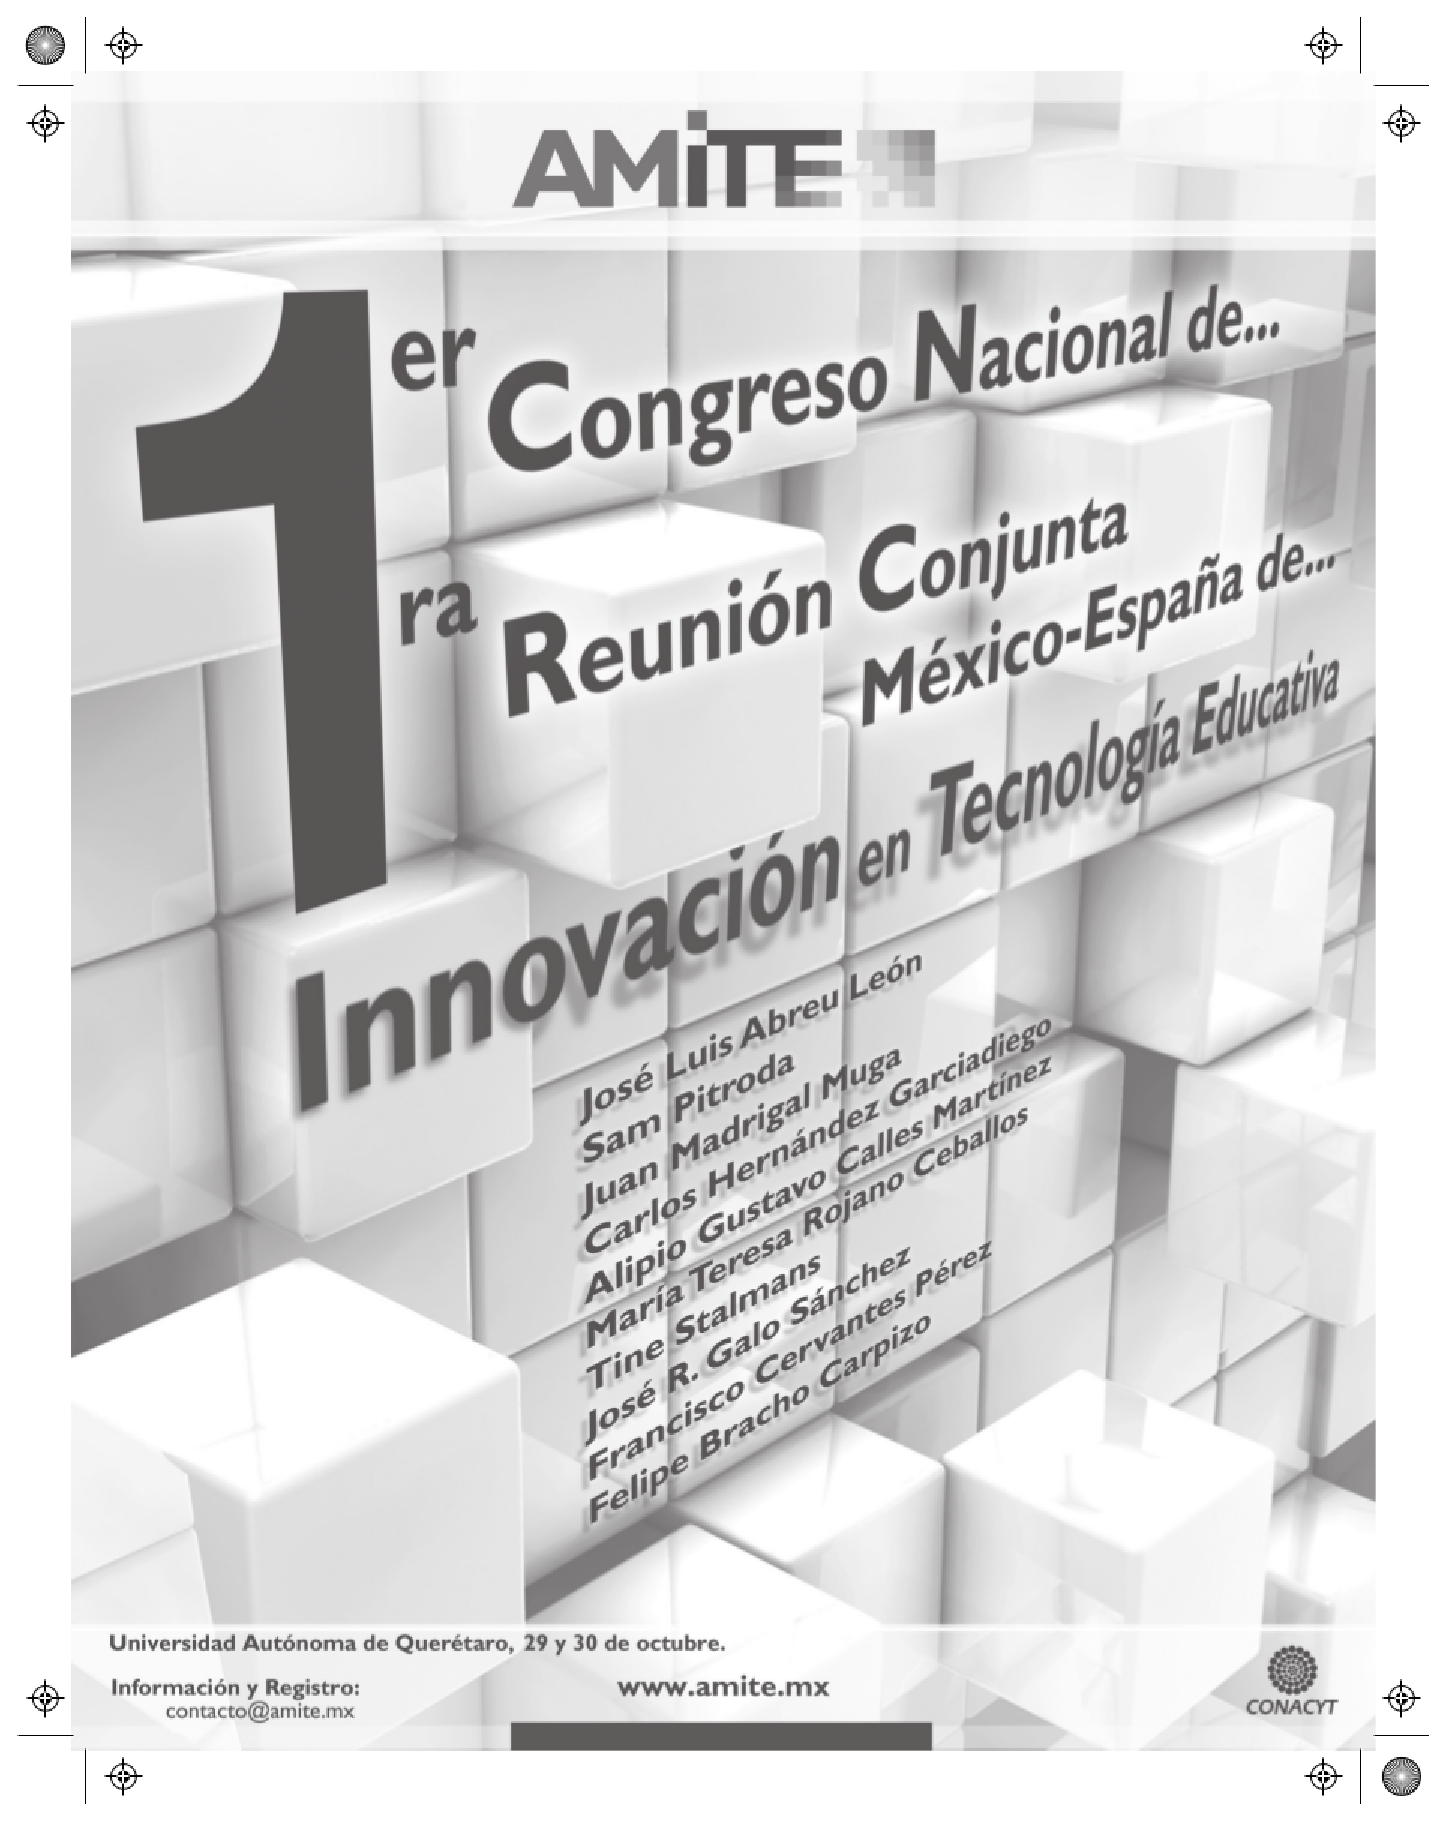
\includegraphics[width=17cm]{otros/cartel_AMITE.eps}
\section{Innovaci�n en Tecnolog�a Educativa}


%%%%%%%%%%%%539%%%%%%%%%%%%
\subsection{Uso de dispositivos m�viles en la ense�anza de la geometr�a: Geolab {\footnotesize (CDV, Bach)}} \label{reg-539} \index{hernandez garciadiego carlos@Hern�ndez Garciadiego Carlos!\ref{reg-539}}
\noindent{\bfseries Carlos Hern�ndez Garciadiego}, {\tt carlosh@unam.mx} {\slshape (Instituto de Matem�ticas, UNAM)}\\
\noindent En esta pl�tica se hablar� de c�mo naci� Geolab y c�mo ha ido
evolucionando para adaptarse al avance de la tecnolog�a desde las
computadoras de escritorio sin conexi�n a Internet hasta los
dispositivos m�viles como las tabletas y los tel�fonos celulares,
pasando por Enciclomedia.Se mostrar� c�mo se hacen construcciones
geom�tricas y lecciones interactivas como soporte para la ense�anza de
la geometr�a y geometr�a anal�tica para diferentes ambientes y
dispositivos

%%%%%%%%%%%%779%%%%%%%%%%%%
\subsection{Matem�TICas versus Innovaci�n {\footnotesize (CPI, Sec)}} \label{reg-779} \index{madrigal muga juan salvador@Madrigal Muga Juan Salvador!\ref{reg-779}}
\noindent{\bfseries Juan Salvador Madrigal Muga}, {\tt juan.madrigal@platea.pntic.mec.es} {\slshape (Proyecto Descartes)}\\
\noindent El Proyecto Descartes permite dar un nuevo enfoque innovador a la
ense�anza y aprendizaje de las Matem�tica en la Ense�anza Secundaria,
bajo la apariencia de un simple cambio de los medios did�cticos este
proyecto persigue un cambio m�s amplio: transformar no solo los medios
y las metodolog�as sino tambi�n los objetivos y los contenidos para
alcanzar el nivel de competencias que requiere la juventud en una
sociedad tecnol�gicamente avanzada.  La propia herramienta Descartes,
en permanente evoluci�n, los contenidos digitales interactivos
producidos con ella y la experimentaci�n llevada a cabo en las aulas
hacen vislumbrar, en un futuro pr�ximo, ese profundo cambio curricular
bajo un nuevo paradigma centrado en el aprendizaje m�s que en la
ense�anza, y ese futuro ser� tanto m�s pr�ximo cuanto antes las
administraciones educativas y entidades responsables de la formaci�n
del profesorado tomen conciencia de la obsolescencia del curr�culo
actual.


%%%%%%%%%%%%1918%%%%%%%%%%%%
\subsection{Innovaci�n en Tecnolog�a Educativa: Caso India {\footnotesize (CPI, Inv)}} \label{reg-1918} \index{pitroda sam@Pitroda Sam!\ref{reg-1918}}
\noindent{\bfseries Sam Pitroda}, {\tt elsy.sirenia@gmail.com} {\slshape (Adviser to the Prime Minister of India on Public Information Infrastructure and Innovations)} \\
\noindent Se expondr� el caso de Innovaci�n Educativa en la India desde
los �ltimos 25 a�os desde la Comisi�n Nacional del
Conocimiento. Se expondr� la agenda digital de la India para los
siguientes 25 a�os.

%%%%%%%%%%%%innmat01%%%%%%%%%%%%
\subsection{Por anunciar} \label{reg-innmat01} \index{calles martinez alipio gustavo@Calles Mart�nez Alipio Gustavo!\ref{reg-innmat01}}
\noindent{\bfseries Alipio Gustavo Calles Mart�nez}, {\tt calles@unam.mx} {\slshape (Facultad de Ciencias, UNAM)}\\


%%%%%%%%%%%%1524%%%%%%%%%%%%
\subsection{El futuro de las tecnolog�as digitales en la educaci�n matem�tica: treinta a�os despu�s de investigaci�n intensiva en el campo {\footnotesize (CPI, Sec)}} \label{reg-1524} \index{rojano ceballos maria teresa@Rojano Ceballos Mar�a Teresa!\ref{reg-1524}}
\noindent{\bfseries Mar�a Teresa Rojano Ceballos}, {\tt trojano@cinvestav.mx} {\slshape (Centro de Investigaci�n y de Estudios Avanzados (Cinvestav) del Instituto Polit�cnico Nacional (IPN) Departamento de Matem�tica Educativa)}\\
\noindent En su conferencia plenaria del 2010, en el congreso del ``17th ICMI
Study: Mathematics Education and Technology-Rethinking the Terrain'',
Seymour Papert se�al� que si bien ha sido importante investigar c�mo
el conocimiento existente puede ser aprendido (y ense�ado) en entornos
tecnol�gicos, ped�a a la audiencia de investigadores que dedic�ramos
un 10\% de nuestras reflexiones durante la reuni�n a considerar qu�
nuevos tipos de pr�cticas y conocimientos matem�ticos podr�an emerger,
como resultado del acceso a un uso efectivo de las tecnolog�as
digitales. Siguiendo el esp�ritu de la sugerencia de Seymour, en esta
ponencia har� una reflexi�n sobre c�mo la evoluci�n tecnol�gica, junto
con la experiencia acumulada de 30 a�os de investigaci�n intensiva
sobre su uso en la educaci�n matem�tica, pueden llegar a influir en el
futuro en el curr�culo oficial y en el curr�culo que en realidad se
implementa en la pr�ctica cotidiana del aula de matem�ticas (enactive
curriculum). M�s all� de la posibilidad de un acceso temprano a ideas
poderosas en matem�ticas que ofrecen los entornos tecnol�gicos de
aprendizaje, sus potencialidades did�cticas probadas (de naturaleza
cognitiva y epistemol�gica) hacen suponer que su influencia podr�a
llegar a moldear un curr�culo de matem�ticas completamente nuevo. Sin
embargo, esta posibilidad ha sido tema de acalorados debates en la
comunidad internacional de matem�ticos y especialistas en educaci�n
matem�tica. En mi presentaci�n, me referir� a dos posturas extremas a
este respecto y tratar� de plantear los pros y los contras de una y de
otra.


%%%%%%%%%%%%841%%%%%%%%%%%%
\subsection{An�lisis sem�ntico de lenguaje natural  con �rboles l�gico-sem�nticos {\footnotesize (RI, Bach)}} \label{reg-841} \index{stalmans tine@Stalmans Tine!\ref{reg-841}}
\noindent{\bfseries Tine Stalmans}, {\tt tinestalmans@gmail.com} {\slshape (Laboratorio para la Innovaci�n en Tecnolog�a Educativa (LITE))}\\
\noindent El proyecto Di�logos Inteligentes tiene como objetivo la
creaci�n de un conjunto de herramientas digitales que permiten que el
usuario (alumno) entable una conversaci�n con un tutor virtual, con el
fin de explorar y aprender alg�n tema de inter�s educativo. Como estos
di�logos se desarrollan a manera de
pregunta-respuesta-retroalimentaci�n (feedback), para que el tutor
virtual pueda dar retroalimentaciones significativas y precisas en
funci�n de las ideas y los conocimientos previos de cada persona, la
elaboraci�n de algoritmos capaces de hacer una ``lectura'' sem�ntica
adecuada de las contestaciones del alumno es una parte fundamental del
proyecto.  En esta ponencia se presentar�n los algoritmos de an�lisis
sem�ntico de lenguaje natural elaborados en el marco de este
proyecto. La metodolog�a elegida consiste en comparar lo que escribe
el usuario con una serie de respuestas esperadas -que pueden ser
correctas, incorrectas o parcialmente correctas-, cuyo significado se
codifica como ``patr�n l�gico-sem�ntico''. Estos patrones est�n
conformados por claves sem�nticas que se unen mediante operadores
l�gicos (AND, OR, NOT, NEG, MAS), formando as� un �rbol binario que
expresa un significado s. Tambi�n se presentar� un algoritmo de
correcci�n de errores ortogr�ficos comunes en espa�ol.

%%%%%%%%%%%%1133%%%%%%%%%%%%
\subsection{Descartes: Asistente y Mediador Metodol�gico {\footnotesize (CDV, Sec)}} \label{reg-1133} \index{galo sanchez jose@Galo S�nchez Jos�!\ref{reg-1133}}
\noindent{\bfseries Jos� Galo S�nchez}, {\tt jose.galo@roble.pntic.mec.es} {\slshape (Ministerio de Educaci�n, Cultura y Deporte (MECD) de Espa�a Proyecto Descartes)}\\
\noindent El proyecto Descartes del Ministerio de Educaci�n, Cultura y
Deporte de Espa�a tiene como objetivo la innovaci�n en la ense�anza y
aprendizaje de las Matem�ticas utilizando las Tecnolog�as de la
Informaci�n y de la Comunicaci�n (TIC). Para la consecuci�n de este
objetivo se dispone de una herramienta, de igual nombre, que ha
permitido el desarrollo de un amplio banco de recursos educativos
interactivos que act�an como asistentes y mediadores que catalizan el
cambio metodol�gico en el aula y contribuyen a la mejora
educativa. Las TIC han introducido un dr�stico y veloz cambio en la
Sociedad. Las pol�ticas globales y las educativas en particular buscan
permeabilizar la Sociedad de la Informaci�n y la de la Formaci�n en la
Sociedad del Conocimiento. La Escuela, s�ntesis intergeneracional,
acoge una brecha tecnol�gica generacional que pone en cuesti�n
metodolog�as y procedimientos de aprendizaje. El paso a aulas
tecnificadas no va aunado con el adecuado cambio metodol�gico, se
introducen nuevos recursos en modelos previamente establecidos y las
experiencias se centran en usos espor�dicos, no sistem�ticos, aislados
y de corta duraci�n. En el contexto educativo se constata y vuelve a
manifestarse la habitual, casi idiosincr�sica, ``Cultura del rechazo''
cuyo germen quiz�s pueda situarse en la no consecuci�n de la necesaria
``invisibilidad tecnol�gica''. En esta ponencia se muestra la diversidad
de los materiales desarrollados con Descartes y se pone de manifiesto
c�mo la utilizaci�n de estos mediadores virtuales favorece globalmente
tanto la formaci�n matem�tica concreta como la abstracta. Se incide
principal y esencialmente en las propuestas metodol�gicas que de
manera natural surgen al usarlos en el aula. Partiendo de ejemplos
donde el recurso se usa s�lo como elemento de representaci�n gr�fica
en modelos tradicionales transmisores -como mera pizarra digital-,
progresivamente se ir� detallando y profundizando en el potencial
did�ctico que la interactividad alumnado-m�quina aporta a la
construcci�n del conocimiento significativo, potenciando
simult�neamente tanto la ``autonom�a personal'', el ``aprender a
aprender'' y la formaci�n competencial. Igualmente se expone c�mo la
utilizaci�n de los recursos de Descartes adentra al profesorado en una
reflexi�n sobre su labor docente y cuestiona acerca de las rutinas
profesionales.


%%%%%%%%%%%%1910%%%%%%%%%%%%
\subsection{El Ciclo Educaci�n-Tecnolog�a {\footnotesize (CPI, Bach)}} \label{reg-1910} \index{cervantes francisco@Cervantes Francisco!\ref{reg-1910}}
\noindent{\bfseries Francisco Cervantes}, {\tt elsa\_sirenia@hotmail.com} {\slshape (Centro de Ciencias Aplicadas y Desarrollo Tecnol�gico (CCADET-UNAM))}\\
\noindent Los Sistemas y Ambientes Educativos requieren, en la
actualidad, de un uso apropiado de las Tecnolog�as Digitales, que
responda a las necesidades planteadas por las nuevas propuestas
emanadas de la Psicolog�a Educativa (Aprendizaje) y la Pedagog�a
(Ense�anza), as� como de las nuevas formas de organizaci�n, y de
gesti�n, de las Instituciones Educativas que demanda una Sociedad de
la Informaci�n, del Conocimiento y del Aprendizaje. En esta pl�tica se
presenta un proyecto donde se establece un Ciclo de interacci�n entre
las �reas de Educaci�n con las de las Tecnolog�as Digitales, para
integra tecnolog�as emergentes (Contenido Abierto, Anal�tica del
Aprendizaje, etc.), en la construcci�n de un espacio de aprendizaje
que apoye, de manera extracurricular, a los estudiantes en el
mejoramiento de su desempe�o acad�mico.

%%%%%%%%%%%%1903%%%%%%%%%%%%
\subsection{Pasado, presente y futuro de proyectos tipo Enciclomedia {\footnotesize (CPI, Pri)}} \label{reg-1903} \index{bracho carpizo felipe@Bracho Carpizo Felipe!\ref{reg-1903}}
\noindent{\bfseries Felipe Bracho Carpizo}, {\tt lillyben@hotmail.com} {\slshape (Direcci�n General de Computo y de Tecnolog�as de la Universidad Aut�noma de M�xico (UNAM))}\\
\noindent Se presentar� el proyecto Enciclomedia que se instal� en
150,000 escuelas de todo el pa�s, y se describir�n las dificultades
por las que pas� y sus principales logros. Se expondr� en especial el
proyecto Ingl�s Enciclomedia, sus logros y sus vicisitudes.
Finalmente se expondr� el nuevo esquema para ordenar recursos
did�cticos digitales alrededor del curr�culum y los beneficios que
puede aportar a los procesos de ense�anza y aprendizaje
      % 26
\chapter*{Mesas Redondas}
\addcontentsline{toc}{section}{Mesas Redondas}
{\footnotesize
\begin{center}
%\begin{tabular}{|p{50pt}|p{50pt}|p{65pt}|p{65pt}|p{65pt}|p{65pt}|p{65pt}|}
\begin{tabular}{|c|c|c|c|c|c|c|}
\hline[1pt]
\multicolumn{7}{|c|}{\Large\bfseries Mesas Redondas p�g. \pageref{mesas01}}\\
\hline
\hline
{\hfill\bfseries Hora\hfill} & {\hfill\bfseries Lunes\hfill} &  \multicolumn{2}{|c|}{\bfseries Martes} & {\hfill\bfseries Mi�rcoles\hfill} & {\hfill\bfseries Jueves\hfill} & {\hfill\bfseries Viernes\hfill} \\
\hline
{\hfill 9:00-9:50 \hfill} &
      &
\multicolumn{2}{|c|}{}    &
    &
        &
      \\
\cline{1-1}\cline{3-7}

{\hfill 10:00-10:20 \hfill} &
    Inauguraci�n   &
\multicolumn{2}{|c|}{}    &
    &
    &
     \\
\cline{1-1}\cline{5-7}

{\hfill 10:20-10:40 \hfill} &
    &
  \multicolumn{2}{|c|}{\bfseries MESA 2}  &
     &
    &
     \\
\cline{1-2}\cline{5-7}

{\hfill 10:40-11:00 \hfill} &
    {\bfseries PLENARIA }  &
  \multicolumn{2}{|c|}{}  &
      &
      &
     \\
\cline{1-1}\cline{4-4}\cline{5-7}

{\hfill 11:00-11:30 \hfill} &
     {\bfseries  1 }&
   \ \ \ \ \ \ \  &
    &
     \multicolumn{3}{|c|} {\bfseries Caf�} \\
\cline{1-2}\cline{5-7}

{\hfill 11:40-12:00 \hfill} &
     Traslado &
      & &
  &
  &
   \\
\cline{1-3}\cline{5-7}

{\hfill 12:00-12:50 \hfill} &
       &
    \multicolumn{2}{|c|}{\bfseries MESA 3[*]}  &
    {\bfseries MESA 5}  &
   &
   \\
\cline{1-1}\cline{5-7}

{\hfill 12:50-13:00 \hfill} &
  {\bfseries MESA 1}  &
  \multicolumn{2}{|c|}{} &
     \multicolumn{3}{|c|} {\bfseries Traslado} \\
\cline{1-1}\cline{3-7}

{\hfill 13:00-13:30 \hfill} &
       &
    \multicolumn{2}{|c|}{\bfseries PLENARIA  } &
    {\bfseries PLENARIA  } &
   {\bfseries PLENARIA  } &
   {\bfseries PLENARIA  } \\
\cline{1-1}

{\hfill 13:30-13:50 \hfill} &
      &
    \multicolumn{2}{|c|}{\bfseries 2  } &
    {\bfseries 3  } &
   {\bfseries 4  } &
   {\bfseries 5  } \\
\hline

{\hfill 14:00-16:30 \hfill} &
     \multicolumn{3}{|c|}{\bfseries COMIDA} &
   &
   \multicolumn{2}{|c|} {\bfseries COMIDA} \\
\cline{1-4}\cline{6-7}

{\hfill 16:40-17:00 \hfill} &
       &
   \multicolumn{2}{|c|}{} &
     &
     &
     \\
\cline{1-2}\cline{6-7}

{\hfill 17:00-17:20 \hfill} &
      &
   \multicolumn{2}{|c|}{}   &
     &
    &
    \\
\cline{1-2}\cline{6-7}

{\hfill 17:20-17:40 \hfill} &
       &
    \multicolumn{2}{|c|}{\bfseries MESA 4}  &
     &
     &
     \\
\cline{1-2}\cline{6-7}

{\hfill 17:40-18:10 \hfill} &
     {\bfseries Caf�} &
 \multicolumn{2}{|c|}{} &
    {\bfseries Tarde Libre} &
     \multicolumn{2}{|c|} {\bfseries Caf�} \\
\cline{1-2}\cline{6-7}

{\hfill 18:10-18:30 \hfill} &
      &
   \multicolumn{2}{|c|}{} &
    &
   {\bfseries PLENARIA  } &
   {\bfseries PLENARIA  } \\
\cline{1-4}

{\hfill 18:30-18:50 \hfill} &
  &
   \multicolumn{2}{|c|}{} &
    &
   {\bfseries 8  } &
 {\bfseries 9  } \\
\cline{1-4}\cline{6-7}

{\hfill 18:50-19:00 \hfill} &
    \multicolumn{3}{|c|} {\bfseries Traslado} &
     &
  {\bfseries HOMENAJE} &
  {\bfseries Traslado}  \\
\cline{1-4}\cline{7-7}
{\hfill 19:00-19:50 \hfill} &
 {\bfseries  PLENARIA 6 } &
  \multicolumn{2}{|c|}  {\bfseries  PLENARIA  7} &
       &
   {\bfseries  JORGE} &
   {\bfseries Asamblea } \\
\cline{1-4}
{\hfill 19:50-20:50  \hfill} &
  {\bfseries  HOMENAJE }&
 \multicolumn{2}{|c|}  {\bfseries  HOMENAJE } &
       &
  {\bfseries  IZE}  &
  {\bfseries  General }  \\
  \cline{1-1}\cline{6-7}
{\hfill 20:50-21:00 \hfill} &
 {\bfseries  ERNESTO }  &
  \multicolumn{2}{|c|}  {\bfseries FRANCISCO} &
       &
  &
   {\bfseries Traslado } \\
\cline{1-1}\cline{6-7}
    {\hfill 21:00-21:50  \hfill} &
 {\bfseries  LACOMBA } &
 \multicolumn{2}{|c|}   {\bfseries RAGGI} &
       &
    &
   {\bfseries Clausura}   \\
\cline{1-7}

\hline[1pt]
\multicolumn{7}{|c|}{\large\bfseries Auditorio Fernando D�az Ram�rez }\\
\multicolumn{7}{|c|}{\bfseries [*] Auditorio Maestro Adolfo Chac\'on }\\
\hline
\end{tabular}
\end{center}

}

\begin{multicols}{2}
\raggedcolumns


%\noindent \ref{mesas04} {\bfseries Las Matem�ticas en el Estado de Quer�taro}\\
\subsection*{\sffamily 1. Las Matem�ticas en el Estado de Quer�taro} \label{mesas04}
\index{pacheco cardenas agustin@Pacheco C�rdenas Agust�n!M1}
\index{diaz barriga alejandro@D�az Barriga Alejandro!M1}
\index{arredondo jose carlos@Arredondo Jos� Carlos!M1}
\index{cabrera munoz dolores@Cabrera Mu�oz Dolores!M1}
\index{gomez gonzalo@G�mez Gonzalo!M1}
\index{perez hermosillo jesus@P�rez Hermosillo Jes�s!M1}
\index{montejano peimbert luis@Montejano Peimbert Luis!M1}
\index{ramirez de leon sotero@Ram�rez de Le�n Sotero!M1}
\noindent
{\slshape Jos� Carlos Arredondo} \\
{\slshape Dolores Cabrera Mu�oz} \\
{\slshape Alejandro D�az Barriga} \\
{\slshape Gonzalo G�mez} \\
{\slshape Luis Montejano Peimbert} \\
{\slshape Agust�n Pacheco C�rdenas} \\
{\slshape Jes�s P�rez Hermosillo} \\
{\slshape Sotero Ram�rez de Le�n} \\
{\bfseries Moderador: }{\slshape Roberto Torres} \\

% Lunes 29 de octubre 12:00 a 13:50



%%%%%%%%%%mesas03%%%%%%%%%%
%\noindent \ref{mesas03} {\bfseries Haciendo camino al andar: Mujeres y Matem�ticas}\\
\subsection*{\sffamily 2. Haciendo camino al andar: Mujeres y Matem�ticas} \label{mesas03}
\index{diaz barriga alejandro@D�az Barriga Alejandro!M2}
\index{balbuena martinez camino@Balbuena Mart�nez Camino!M2}
\index{loaiza maribel@Loaiza Maribel!M2}
\index{olsen mika@Olsen Mika!M2}
\index{rumbos beatriz@Rumbos Beatr�z!M2}
\index{saavedra barrera patricia@Saavedra Barrera Patricia!M2}
\index{sosa carmen@Sosa Carmen!M2}
\noindent
{\slshape Beatr�z Rumbos} \\
{\slshape Camino Balbuena} \\
{\slshape Carmen Sosa} \\
{\slshape Maribel Loaiza} \\
{\slshape Mika Olsen} \\
{\slshape Patricia Saavedra} \\
{\bfseries Moderador: }{\slshape Alejandro D�az Barriga} \\

%% Martes 30 de octubre de 2012, 10:00 a.m. a 12:00 p.m.

\columnbreak

%%%%%%%%%%mesas02%%%%%%%%%%
%% \noindent \ref{mesas02} {\bfseries Los matem�ticos en el sector p�blico}\\
\subsection*{\sffamily 3. Los matem�ticos en el sector p�blico [*]} \label{mesas02}
\index{sanchez arroyo abdon@S�nchez Arroyo Abd�n!M3}
\index{velasco hernandez jorge x@Velasco Hern�ndez Jorge X!\;M3}
\index{sangines luis m@Sangin�s Luis M.!M3}
\index{covarrubias jaramillo enrique@Covarrubias Jaramillo Enrique!\;M3}
\noindent
{\slshape Abd�n S�nchez Arroyo} \\
{\slshape Jorge X. Velasco Hern�ndez} \\
{\slshape Luis M. Sangin�s} \\
{\bfseries Moderador: }{\slshape Enrique Covarrubias Jaramillo} \\

%% martes 30 de octubre a las 12


%%%%%%%%%%mesas01%%%%%%%%%%
%\noindent \ref{mesas01} {\bfseries Mujeres Matem�ticas: Realidad, acciones y perspectivas}\\
\subsection*{\sffamily 4. Mujeres Matem�ticas: Realidad, acciones y perspectivas} \label{mesas01}
\index{luviano johana@Luviano Johana!M4}
\index{manjarrez gutierrez fabiola@Manjarrez Guti�rrez Fabiola!\;M4}
\index{puga isabel@Puga Isabel!M4}
\index{rojano teresa@Rojano Teresa!M4}
\index{ursini sonia@Ursini Sonia!M4}
\index{tellez mara@T�llez Mara!M4}
\index{caballero acosta maria emilia@Caballero Acosta Mar�a Emilia!\;M4}
\noindent
{\slshape Johana Luviano} \\
{\slshape Fabiola Manjarrez} \\
{\slshape Isabel Puga} \\
{\slshape Teresa Rojano} \\
{\slshape Sonia Ursini} \\
{\bfseries Moderadora: }{\slshape Mar�a Emilia Caballero} \\

%% Martes 30, 16:40 p.m. A 18:30 p.m.

%%%%%%%%%%mesas05%%%%%%%%%%
%\noindent \ref{mesas05} {\bfseries Nuestro Sistema Educativo: Naturaleza y Desaf�os}\\
\subsection*{\sffamily 5. Nuestro Sistema Educativo: Naturaleza y Desaf�os} \label{mesas05}
%\index{zorrilla fierro margarita@Zorrilla Fierro Margarita!M5}
%\index{didriksoon takayanagui axel@Didriksoon Takayanagui Axel!M5}
\index{robles Vasquez hector@Robles V\'asquez H\'ector!M5}
\index{rubio ramirez santiago@Rubio Ram\'irez Santiago!M5}
\index{mercado sanchez gema@Mercado S�nchez Gema!M5}
\index{dolores flores crisologo@Dolores Flores Cris�logo!M5}
\noindent
%{\slshape Margarita Zorrilla Fierro} \\
%{\slshape Axel Didriksoon Takayanagui} \\
{\slshape H�ctor Robles V�squez} \\
{\slshape Santiago Rubio Ram\'irez} \\
{\slshape Gema Mercado S�nchez} \\
{\slshape Cris�logo Dolores Flores} \\
{\bfseries Moderadora: }{\slshape Rosa Mar�a Farf�n} \\

% Mi�rcoles 31 de octubre 12:00 a 12:50


\end{multicols}

\chapter*{Sesiones Especiales}
\addcontentsline{toc}{section}{Sesiones Especiales}
{\footnotesize
\begin{center}
%\begin{tabular}{|p{50pt}|p{50pt}|p{65pt}|p{65pt}|p{65pt}|p{65pt}|p{65pt}|}
\begin{tabular}{|c|c|c|c|c|c|}
\hline[1pt]
\multicolumn{6}{|c|}{\Large\bfseries Din�mica Hamiltoniana: teor�a y aplicaciones p�g. \pageref{reg-1510}}\\
\hline
\hline
{\hfill\bfseries Hora\hfill} & {\hfill\bfseries Lunes\hfill} &  {\hfill\bfseries Martes\hfill} & {\hfill\bfseries Mi�rcoles\hfill} & {\hfill\bfseries Jueves\hfill} & {\hfill\bfseries Viernes\hfill} \\
\hline
{\hfill 9:00-9:50 \hfill} &
      &
    &
    &
        &
      \\
\cline{1-1}\cline{3-6}

{\hfill 10:00-10:20 \hfill} &
    Inauguraci�n   &
   {\bfseries \ref{reg-1510}} &
    &
    &
     \\
\cline{1-1}\cline{3-6}

{\hfill 10:20-10:40 \hfill} &
    &
   {\bfseries \ref{reg-854}} &
     &
    &
     \\
\cline{1-6}

{\hfill 10:40-11:00 \hfill} &
      &
   {\bfseries \ref{reg-1032}} &
      &
      &
     \\
\cline{1-1}\cline{3-6}

{\hfill 11:00-11:30 \hfill} &
     {\bfseries PLENARIA 1 }&
     \multicolumn{4}{|c|} {\bfseries Caf�} \\
\cline{1-6}

{\hfill 11:40-12:00 \hfill} &
     Traslado &
     {\bfseries \ref{reg-1038}} &
  &
  &
   \\
\cline{1-6}

{\hfill 12:00-12:50 \hfill} &
       &
      &
      &
   &
   \\
\cline{1-6}

{\hfill 12:50-13:00 \hfill} &
     \multicolumn{5}{|c|} {\bfseries Traslado} \\
\cline{1-6}

{\hfill 13:00-13:30 \hfill} &
       &
    {\bfseries PLENARIA  } &
    {\bfseries PLENARIA  } &
   {\bfseries PLENARIA  } &
   {\bfseries PLENARIA  } \\
%\cline{1-2}

{\hfill 13:30-13:50 \hfill} &
      &
    {\bfseries 2  } &
    {\bfseries 3  } &
   {\bfseries 4  } &
   {\bfseries 5  } \\
\cline{1-6}

{\hfill 14:00-16:30 \hfill} &
    \multicolumn{2}{|c|} {\bfseries COMIDA} &
   &
   \multicolumn{2}{|c|} {\bfseries COMIDA} \\
\cline{1-3}\cline{5-6}

{\hfill 16:40-17:00 \hfill} &
       &
   {\bfseries \ref{reg-1093}} &
     &
     &
     \\
\cline{1-1}\cline{3-3}\cline{5-6}

{\hfill 17:00-17:20 \hfill} &
      &
     {\bfseries \ref{reg-1213}} &
     &
    &
    \\
\cline{1-1}\cline{3-3}\cline{5-6}

{\hfill 17:20-17:40 \hfill} &
       &
     {\bfseries \ref{reg-1680}} &
     &
     &
     \\
\cline{1-3}\cline{5-6}

{\hfill 17:40-18:10 \hfill} &
     \multicolumn{2}{|c|} {\bfseries Caf�}&
    {\bfseries Tarde Libre} &
     \multicolumn{2}{|c|} {\bfseries Caf�} \\
\cline{1-3}\cline{5-6}

{\hfill 18:10-18:30 \hfill} &
      &
   {\bfseries \ref{reg-1192}} &
    &
   {\bfseries PLENARIA  } &
   {\bfseries PLENARIA  } \\
\cline{1-3}

{\hfill 18:30-18:50 \hfill} &
  &
    &
    &
   {\bfseries 8  } &
 {\bfseries 9  } \\
\cline{1-3}\cline{5-6}

{\hfill 18:50-19:00 \hfill} &
    \multicolumn{2}{|c|} {\bfseries Traslado} &
     &
  {\bfseries HOMENAJE} &
  {\bfseries Traslado}  \\
\cline{1-3}\cline{6-6}
{\hfill 19:00-19:50 \hfill} &
 {\bfseries  PLENARIA 6 } &
   {\bfseries  PLENARIA  7} &
       &
   {\bfseries  JORGE} &
   {\bfseries Asamblea } \\
\cline{1-3}
{\hfill 19:50-20:50  \hfill} &
  {\bfseries  HOMENAJE }&
  {\bfseries  HOMENAJE } &
       &
  {\bfseries  IZE}  &
  {\bfseries  General }  \\
  \cline{1-1}\cline{5-6}
{\hfill 20:50-21:00 \hfill} &
 {\bfseries  ERNESTO }  &
   {\bfseries FRANCISCO} &
       &
  &
   {\bfseries Traslado } \\
\cline{1-1}\cline{5-6}
    {\hfill 21:00-21:50  \hfill} &
 {\bfseries  LACOMBA } &
   {\bfseries RAGGI} &
       &
    &
   {\bfseries Clausura}   \\
\cline{1-6}

\hline[1pt]
\multicolumn{6}{|c|}{\large\bfseries Sal�n I9 }\\
\hline
\end{tabular}
\end{center}

}

\begin{multicols}{2}
\raggedcolumns

%%%%%%%%%%1510%%%%%%%%%%
\noindent \ref{reg-1510} {\bfseries Din�mica en la DNLSE  y modelos afines}\\
{\slshape Carlos Leopoldo Pando Lambruschini} {\footnotesize (RI, Inv)}\\

%%%%%%%%%%854%%%%%%%%%%
\noindent \ref{reg-854} {\bfseries Sistemas perturbados: ser lineal o bifurcar en el intento y \'erase una vez el \'indice de Conley}\\
{\slshape Nancy Leticia Gonz�lez Morales} {\footnotesize (RI, Inv)}\\

%%%%%%%%%%1032%%%%%%%%%%
\noindent \ref{reg-1032} {\bfseries Aproximaci�n por �ptica geom�trica para la transferencia y captura de exceso de electrones}\\
{\slshape Luis Alberto Cisneros Ake} {\footnotesize (RI, Inv)}\\

%%%%%%%%%%1038%%%%%%%%%%
\noindent \ref{reg-1038} {\bfseries Estabilizaci�n por resonancia param�trica del levitr\'on}\\
{\slshape Arturo Olvera Ch�vez} {\footnotesize (RI, Inv)}\\

%%%%%%%%%%1093%%%%%%%%%%
\noindent \ref{reg-1093} {\bfseries Estabilidad de los equilibrios relativos piramidales en el problema curvado de los  $4$--cuerpos con curvatura positiva}\\
{\slshape Ernesto P�rez-Chavela} {\footnotesize (RI, Inv)}\\

%%%%%%%%%%1213%%%%%%%%%%
\noindent \ref{reg-1213} {\bfseries Geometr�a en la ecuaci�n de Sine-Gordon}\\
{\slshape Gustavo Cruz-Pacheco} {\footnotesize (RI, Inv)}\\

%%%%%%%%%%1680%%%%%%%%%%
\noindent \ref{reg-1680} {\bfseries Teor�a KAM en cadenas Hamiltonianas}\\
{\slshape Jorge Viveros Rogel} {\footnotesize (RI, Inv)}\\

%%%%%%%%%%1192%%%%%%%%%%
\noindent \ref{reg-1192} {\bfseries Localizaci�n espacial en cadenas nolineales}\\
{\slshape Panayiotis Panayotaros, Francisco Mart�nez} {\footnotesize (RI, Inv)}\\

\end{multicols}

{\footnotesize
\begin{center}
%\begin{tabular}{|p{50pt}|p{50pt}|p{65pt}|p{65pt}|p{65pt}|p{65pt}|p{65pt}|}
\begin{tabular}{|c|c|c|c|c|c|}
\hline[1pt]
\multicolumn{6}{|c|}{\Large\bfseries XVII Encuentro de Escuelas Matem�ticas}\\
\hline
\hline
{\hfill\bfseries Hora\hfill} & {\hfill\bfseries Lunes\hfill} &  {\hfill\bfseries Martes\hfill} & {\hfill\bfseries Mi�rcoles\hfill} & {\hfill\bfseries Jueves\hfill} & {\hfill\bfseries Viernes\hfill} \\
\hline
{\hfill 9:00-9:50 \hfill} &
      &
    &
    &
        &
      \\
\cline{1-1}\cline{3-6}

{\hfill 10:00-10:20 \hfill} &
    Inauguraci�n   &
    &
    &
    &
     \\
\cline{1-1}\cline{3-6}

{\hfill 10:20-10:40 \hfill} &
    &
    &
     &
    &
     \\
\cline{1-6}

{\hfill 10:40-11:00 \hfill} &
      &
    &
      &
      &
     \\
\cline{1-1}\cline{3-6}

{\hfill 11:00-11:30 \hfill} &
     {\bfseries PLENARIA 1 }&
     \multicolumn{4}{|c|} {\bfseries Caf�} \\
\cline{1-6}

{\hfill 11:40-12:00 \hfill} &
     Traslado &
      &
  &
  &
   \\
\cline{1-6}

{\hfill 12:00-12:50 \hfill} &
       &
      &
      &
   &
   \\
\cline{1-6}

{\hfill 12:50-13:00 \hfill} &
     \multicolumn{5}{|c|} {\bfseries Traslado} \\
\cline{1-6}

{\hfill 13:00-13:30 \hfill} &
       &
    {\bfseries PLENARIA  } &
    {\bfseries PLENARIA  } &
   {\bfseries PLENARIA  } &
   {\bfseries PLENARIA  } \\
%\cline{1-2}

{\hfill 13:30-13:50 \hfill} &
      &
    {\bfseries 2  } &
    {\bfseries 3  } &
   {\bfseries 4  } &
   {\bfseries 5  } \\
\cline{1-6}

{\hfill 14:00-16:30 \hfill} &
    \multicolumn{2}{|c|} {\bfseries COMIDA} &
   &
   \multicolumn{2}{|c|} {\bfseries COMIDA} \\
\cline{1-3}\cline{5-6}

{\hfill 16:40-17:00 \hfill} &
   {\bfseries XVII Encuentro}    &
    &
     &
     &
     \\
\cline{1-1}\cline{3-3}\cline{5-6}

{\hfill 17:00-17:20 \hfill} &
     {\bfseries de Escuelas} &
      &
     &
    &
    \\
\cline{1-1}\cline{3-3}\cline{5-6}

{\hfill 17:20-17:40 \hfill} &
     {\bfseries Matem�ticas}  &
      &
     &
     &
     \\
\cline{1-3}\cline{5-6}

{\hfill 17:40-18:10 \hfill} &
     \multicolumn{2}{|c|} {\bfseries Caf�}&
    {\bfseries Tarde Libre} &
     \multicolumn{2}{|c|} {\bfseries Caf�} \\
\cline{1-3}\cline{5-6}

{\hfill 18:10-18:30 \hfill} &
     {\bfseries XVII Encuentro de} &
    &
    &
   {\bfseries PLENARIA  } &
   {\bfseries PLENARIA  } \\
\cline{1-1}\cline{3-3}

{\hfill 18:30-18:50 \hfill} &
 {\bfseries Escuelas Matem�ticas} &
    &
    &
   {\bfseries 8  } &
 {\bfseries 9  } \\
\cline{1-3}\cline{5-6}

{\hfill 18:50-19:00 \hfill} &
    \multicolumn{2}{|c|} {\bfseries Traslado} &
     &
  {\bfseries Traslado} &
    \\
\cline{1-3}\cline{5-5}

{\hfill 19:00-19:50 \hfill} &
 {\bfseries PLENARIA 6 } &
   {\bfseries PLENARIA  7} &
       &
   {\bfseries Asamblea General } &
   {\bfseries Clausura } \\
\cline{1-6}

\hline[1pt]
\multicolumn{6}{|c|}{\large\bfseries Sal�n I9 }\\
\hline
\end{tabular}
\end{center}

}

\begin{multicols}{2}
\raggedcolumns



%%%%%%%%%%encesc01%%%%%%%%%%
\noindent \ref{encesc01} {\bfseries Presentaci�n} \\


%%%%%%%%%%encesc02%%%%%%%%%%
\noindent \ref{encesc02} {\bfseries An�lisis, discusi�n y acuerdo sobre el car�cter de la Organizaci�n Nacional de Instituciones de Matem�ticas (ONIM); y v�nculos con otros comit�s} \\


%%%%%%%%%%encesc03%%%%%%%%%%
\noindent \ref{encesc03} {\bfseries Art�culo de ONIM en reforma de estatutos de la SMM que considere acuerdos tomados y relaciones con otros comit�s} \\


%%%%%%%%%%encesc04%%%%%%%%%%
\noindent \ref{encesc04} {\bfseries Elecci�n de responsables y mecanismos de trabajo y reuniones del comit� y sus coordinadores} \\


%%%%%%%%%%encesc05%%%%%%%%%%
\noindent \ref{encesc05} {\bfseries Inventario de recursos humanos e infraestructura} \\


%%%%%%%%%%encesc06%%%%%%%%%%
\noindent \ref{encesc06} {\bfseries Programa de capacitaci�n nacional y conferencias a distancia} \\


%%%%%%%%%%encesc07%%%%%%%%%%
\noindent \ref{encesc07} {\bfseries Portal y Red Inernet, Red de Capacitadores} \\


%%%%%%%%%%encesc08%%%%%%%%%%
\noindent \ref{encesc08} {\bfseries Evaluaciones y Acreditaciones; CAPEM} \\


%%%%%%%%%%encesc09%%%%%%%%%%
\noindent \ref{encesc09} {\bfseries Bibliotecas m�nimas} \\


%%%%%%%%%%encesc10%%%%%%%%%%
\noindent \ref{encesc10} {\bfseries Proyecto CONACYT sobre redes tem�ticas y convenios} \\


%%%%%%%%%%encesc11%%%%%%%%%%
\noindent \ref{encesc11} {\bfseries Asuntos generales} \\



\end{multicols}
\vfill
%\section{Innovaci�n en Tecnolog�a Educativa}


%%%%%%%%%%%%539%%%%%%%%%%%%
\subsection{Uso de dispositivos m�viles en la ense�anza de la geometr�a: Geolab {\footnotesize (CDV, Bach)}} \label{reg-539} \index{hernandez garciadiego carlos@Hern�ndez Garciadiego Carlos!\ref{reg-539}}
\noindent{\bfseries Carlos Hern�ndez Garciadiego}, {\tt carlosh@unam.mx} {\slshape (Instituto de Matem�ticas, UNAM)}\\
\noindent En esta pl�tica se hablar� de c�mo naci� Geolab y c�mo ha ido
evolucionando para adaptarse al avance de la tecnolog�a desde las
computadoras de escritorio sin conexi�n a Internet hasta los
dispositivos m�viles como las tabletas y los tel�fonos celulares,
pasando por Enciclomedia.Se mostrar� c�mo se hacen construcciones
geom�tricas y lecciones interactivas como soporte para la ense�anza de
la geometr�a y geometr�a anal�tica para diferentes ambientes y
dispositivos

%%%%%%%%%%%%779%%%%%%%%%%%%
\subsection{Matem�TICas versus Innovaci�n {\footnotesize (CPI, Sec)}} \label{reg-779} \index{madrigal muga juan salvador@Madrigal Muga Juan Salvador!\ref{reg-779}}
\noindent{\bfseries Juan Salvador Madrigal Muga}, {\tt juan.madrigal@platea.pntic.mec.es} {\slshape (Proyecto Descartes)}\\
\noindent El Proyecto Descartes permite dar un nuevo enfoque innovador a la
ense�anza y aprendizaje de las Matem�tica en la Ense�anza Secundaria,
bajo la apariencia de un simple cambio de los medios did�cticos este
proyecto persigue un cambio m�s amplio: transformar no solo los medios
y las metodolog�as sino tambi�n los objetivos y los contenidos para
alcanzar el nivel de competencias que requiere la juventud en una
sociedad tecnol�gicamente avanzada.  La propia herramienta Descartes,
en permanente evoluci�n, los contenidos digitales interactivos
producidos con ella y la experimentaci�n llevada a cabo en las aulas
hacen vislumbrar, en un futuro pr�ximo, ese profundo cambio curricular
bajo un nuevo paradigma centrado en el aprendizaje m�s que en la
ense�anza, y ese futuro ser� tanto m�s pr�ximo cuanto antes las
administraciones educativas y entidades responsables de la formaci�n
del profesorado tomen conciencia de la obsolescencia del curr�culo
actual.


%%%%%%%%%%%%1918%%%%%%%%%%%%
\subsection{Innovaci�n en Tecnolog�a Educativa: Caso India {\footnotesize (CPI, Inv)}} \label{reg-1918} \index{pitroda sam@Pitroda Sam!\ref{reg-1918}}
\noindent{\bfseries Sam Pitroda}, {\tt elsy.sirenia@gmail.com} {\slshape (Adviser to the Prime Minister of India on Public Information Infrastructure and Innovations)} \\
\noindent Se expondr� el caso de Innovaci�n Educativa en la India desde
los �ltimos 25 a�os desde la Comisi�n Nacional del
Conocimiento. Se expondr� la agenda digital de la India para los
siguientes 25 a�os.

%%%%%%%%%%%%innmat01%%%%%%%%%%%%
\subsection{Por anunciar} \label{reg-innmat01} \index{calles martinez alipio gustavo@Calles Mart�nez Alipio Gustavo!\ref{reg-innmat01}}
\noindent{\bfseries Alipio Gustavo Calles Mart�nez}, {\tt calles@unam.mx} {\slshape (Facultad de Ciencias, UNAM)}\\


%%%%%%%%%%%%1524%%%%%%%%%%%%
\subsection{El futuro de las tecnolog�as digitales en la educaci�n matem�tica: treinta a�os despu�s de investigaci�n intensiva en el campo {\footnotesize (CPI, Sec)}} \label{reg-1524} \index{rojano ceballos maria teresa@Rojano Ceballos Mar�a Teresa!\ref{reg-1524}}
\noindent{\bfseries Mar�a Teresa Rojano Ceballos}, {\tt trojano@cinvestav.mx} {\slshape (Centro de Investigaci�n y de Estudios Avanzados (Cinvestav) del Instituto Polit�cnico Nacional (IPN) Departamento de Matem�tica Educativa)}\\
\noindent En su conferencia plenaria del 2010, en el congreso del ``17th ICMI
Study: Mathematics Education and Technology-Rethinking the Terrain'',
Seymour Papert se�al� que si bien ha sido importante investigar c�mo
el conocimiento existente puede ser aprendido (y ense�ado) en entornos
tecnol�gicos, ped�a a la audiencia de investigadores que dedic�ramos
un 10\% de nuestras reflexiones durante la reuni�n a considerar qu�
nuevos tipos de pr�cticas y conocimientos matem�ticos podr�an emerger,
como resultado del acceso a un uso efectivo de las tecnolog�as
digitales. Siguiendo el esp�ritu de la sugerencia de Seymour, en esta
ponencia har� una reflexi�n sobre c�mo la evoluci�n tecnol�gica, junto
con la experiencia acumulada de 30 a�os de investigaci�n intensiva
sobre su uso en la educaci�n matem�tica, pueden llegar a influir en el
futuro en el curr�culo oficial y en el curr�culo que en realidad se
implementa en la pr�ctica cotidiana del aula de matem�ticas (enactive
curriculum). M�s all� de la posibilidad de un acceso temprano a ideas
poderosas en matem�ticas que ofrecen los entornos tecnol�gicos de
aprendizaje, sus potencialidades did�cticas probadas (de naturaleza
cognitiva y epistemol�gica) hacen suponer que su influencia podr�a
llegar a moldear un curr�culo de matem�ticas completamente nuevo. Sin
embargo, esta posibilidad ha sido tema de acalorados debates en la
comunidad internacional de matem�ticos y especialistas en educaci�n
matem�tica. En mi presentaci�n, me referir� a dos posturas extremas a
este respecto y tratar� de plantear los pros y los contras de una y de
otra.


%%%%%%%%%%%%841%%%%%%%%%%%%
\subsection{An�lisis sem�ntico de lenguaje natural  con �rboles l�gico-sem�nticos {\footnotesize (RI, Bach)}} \label{reg-841} \index{stalmans tine@Stalmans Tine!\ref{reg-841}}
\noindent{\bfseries Tine Stalmans}, {\tt tinestalmans@gmail.com} {\slshape (Laboratorio para la Innovaci�n en Tecnolog�a Educativa (LITE))}\\
\noindent El proyecto Di�logos Inteligentes tiene como objetivo la
creaci�n de un conjunto de herramientas digitales que permiten que el
usuario (alumno) entable una conversaci�n con un tutor virtual, con el
fin de explorar y aprender alg�n tema de inter�s educativo. Como estos
di�logos se desarrollan a manera de
pregunta-respuesta-retroalimentaci�n (feedback), para que el tutor
virtual pueda dar retroalimentaciones significativas y precisas en
funci�n de las ideas y los conocimientos previos de cada persona, la
elaboraci�n de algoritmos capaces de hacer una ``lectura'' sem�ntica
adecuada de las contestaciones del alumno es una parte fundamental del
proyecto.  En esta ponencia se presentar�n los algoritmos de an�lisis
sem�ntico de lenguaje natural elaborados en el marco de este
proyecto. La metodolog�a elegida consiste en comparar lo que escribe
el usuario con una serie de respuestas esperadas -que pueden ser
correctas, incorrectas o parcialmente correctas-, cuyo significado se
codifica como ``patr�n l�gico-sem�ntico''. Estos patrones est�n
conformados por claves sem�nticas que se unen mediante operadores
l�gicos (AND, OR, NOT, NEG, MAS), formando as� un �rbol binario que
expresa un significado s. Tambi�n se presentar� un algoritmo de
correcci�n de errores ortogr�ficos comunes en espa�ol.

%%%%%%%%%%%%1133%%%%%%%%%%%%
\subsection{Descartes: Asistente y Mediador Metodol�gico {\footnotesize (CDV, Sec)}} \label{reg-1133} \index{galo sanchez jose@Galo S�nchez Jos�!\ref{reg-1133}}
\noindent{\bfseries Jos� Galo S�nchez}, {\tt jose.galo@roble.pntic.mec.es} {\slshape (Ministerio de Educaci�n, Cultura y Deporte (MECD) de Espa�a Proyecto Descartes)}\\
\noindent El proyecto Descartes del Ministerio de Educaci�n, Cultura y
Deporte de Espa�a tiene como objetivo la innovaci�n en la ense�anza y
aprendizaje de las Matem�ticas utilizando las Tecnolog�as de la
Informaci�n y de la Comunicaci�n (TIC). Para la consecuci�n de este
objetivo se dispone de una herramienta, de igual nombre, que ha
permitido el desarrollo de un amplio banco de recursos educativos
interactivos que act�an como asistentes y mediadores que catalizan el
cambio metodol�gico en el aula y contribuyen a la mejora
educativa. Las TIC han introducido un dr�stico y veloz cambio en la
Sociedad. Las pol�ticas globales y las educativas en particular buscan
permeabilizar la Sociedad de la Informaci�n y la de la Formaci�n en la
Sociedad del Conocimiento. La Escuela, s�ntesis intergeneracional,
acoge una brecha tecnol�gica generacional que pone en cuesti�n
metodolog�as y procedimientos de aprendizaje. El paso a aulas
tecnificadas no va aunado con el adecuado cambio metodol�gico, se
introducen nuevos recursos en modelos previamente establecidos y las
experiencias se centran en usos espor�dicos, no sistem�ticos, aislados
y de corta duraci�n. En el contexto educativo se constata y vuelve a
manifestarse la habitual, casi idiosincr�sica, ``Cultura del rechazo''
cuyo germen quiz�s pueda situarse en la no consecuci�n de la necesaria
``invisibilidad tecnol�gica''. En esta ponencia se muestra la diversidad
de los materiales desarrollados con Descartes y se pone de manifiesto
c�mo la utilizaci�n de estos mediadores virtuales favorece globalmente
tanto la formaci�n matem�tica concreta como la abstracta. Se incide
principal y esencialmente en las propuestas metodol�gicas que de
manera natural surgen al usarlos en el aula. Partiendo de ejemplos
donde el recurso se usa s�lo como elemento de representaci�n gr�fica
en modelos tradicionales transmisores -como mera pizarra digital-,
progresivamente se ir� detallando y profundizando en el potencial
did�ctico que la interactividad alumnado-m�quina aporta a la
construcci�n del conocimiento significativo, potenciando
simult�neamente tanto la ``autonom�a personal'', el ``aprender a
aprender'' y la formaci�n competencial. Igualmente se expone c�mo la
utilizaci�n de los recursos de Descartes adentra al profesorado en una
reflexi�n sobre su labor docente y cuestiona acerca de las rutinas
profesionales.


%%%%%%%%%%%%1910%%%%%%%%%%%%
\subsection{El Ciclo Educaci�n-Tecnolog�a {\footnotesize (CPI, Bach)}} \label{reg-1910} \index{cervantes francisco@Cervantes Francisco!\ref{reg-1910}}
\noindent{\bfseries Francisco Cervantes}, {\tt elsa\_sirenia@hotmail.com} {\slshape (Centro de Ciencias Aplicadas y Desarrollo Tecnol�gico (CCADET-UNAM))}\\
\noindent Los Sistemas y Ambientes Educativos requieren, en la
actualidad, de un uso apropiado de las Tecnolog�as Digitales, que
responda a las necesidades planteadas por las nuevas propuestas
emanadas de la Psicolog�a Educativa (Aprendizaje) y la Pedagog�a
(Ense�anza), as� como de las nuevas formas de organizaci�n, y de
gesti�n, de las Instituciones Educativas que demanda una Sociedad de
la Informaci�n, del Conocimiento y del Aprendizaje. En esta pl�tica se
presenta un proyecto donde se establece un Ciclo de interacci�n entre
las �reas de Educaci�n con las de las Tecnolog�as Digitales, para
integra tecnolog�as emergentes (Contenido Abierto, Anal�tica del
Aprendizaje, etc.), en la construcci�n de un espacio de aprendizaje
que apoye, de manera extracurricular, a los estudiantes en el
mejoramiento de su desempe�o acad�mico.

%%%%%%%%%%%%1903%%%%%%%%%%%%
\subsection{Pasado, presente y futuro de proyectos tipo Enciclomedia {\footnotesize (CPI, Pri)}} \label{reg-1903} \index{bracho carpizo felipe@Bracho Carpizo Felipe!\ref{reg-1903}}
\noindent{\bfseries Felipe Bracho Carpizo}, {\tt lillyben@hotmail.com} {\slshape (Direcci�n General de Computo y de Tecnolog�as de la Universidad Aut�noma de M�xico (UNAM))}\\
\noindent Se presentar� el proyecto Enciclomedia que se instal� en
150,000 escuelas de todo el pa�s, y se describir�n las dificultades
por las que pas� y sus principales logros. Se expondr� en especial el
proyecto Ingl�s Enciclomedia, sus logros y sus vicisitudes.
Finalmente se expondr� el nuevo esquema para ordenar recursos
did�cticos digitales alrededor del curr�culum y los beneficios que
puede aportar a los procesos de ense�anza y aprendizaje
      % 26
{\footnotesize
\begin{center}
%\begin{tabular}{|p{50pt}|p{50pt}|p{65pt}|p{65pt}|p{65pt}|p{65pt}|p{65pt}|}
\begin{tabular}{|c|c|c|c|c|c|}
\hline[1pt]
\multicolumn{6}{|c|}{\Large\bfseries La SMM en el Bachillerato p�g. \pageref{reg-1898}}\\
\hline
\hline
{\hfill\bfseries Hora\hfill} & {\hfill\bfseries Lunes\hfill} &  {\hfill\bfseries Martes\hfill} & {\hfill\bfseries Mi�rcoles\hfill} & {\hfill\bfseries Jueves\hfill} & {\hfill\bfseries Viernes\hfill} \\
\hline
{\hfill 9:00-9:50 \hfill} &
      &
    {\bfseries \ref{reg-1892}} &
    {\bfseries \ref{reg-1894}} &
        &
      \\
\cline{1-1}\cline{3-6}

{\hfill 10:00-10:20 \hfill} &
    Inauguraci�n   &
    &
    &
    &
     \\
\cline{1-1}\cline{4-6}

{\hfill 10:20-10:40 \hfill} &
    &
   {\bfseries \ref{reg-1893}} &
     &
    &
     \\
\cline{1-2}\cline{4-6}

{\hfill 10:40-11:00 \hfill} &
      &
    &
      &
      &
     \\
\cline{1-1}\cline{3-6}

{\hfill 11:00-11:30 \hfill} &
     {\bfseries PLENARIA 1 }&
     \multicolumn{4}{|c|} {\bfseries Caf�} \\
\cline{1-6}

{\hfill 11:40-12:00 \hfill} &
     Traslado &
      &
  &
  &
   \\
\cline{1-6}

{\hfill 12:00-12:50 \hfill} &
     {\bfseries \ref{reg-1898}}  &
     {\bfseries \ref{reg-1900}} &
      &
   &
   \\
\cline{1-6}

{\hfill 12:50-13:00 \hfill} &
     \multicolumn{5}{|c|} {\bfseries Traslado} \\
\cline{1-6}

{\hfill 13:00-13:30 \hfill} &
       &
    {\bfseries PLENARIA  } &
    {\bfseries PLENARIA  } &
   {\bfseries PLENARIA  } &
   {\bfseries PLENARIA  } \\
%\cline{1-2}

{\hfill 13:30-13:50 \hfill} &
     {\bfseries \ref{reg-1897}} &
    {\bfseries 2  } &
    {\bfseries 3  } &
   {\bfseries 4  } &
   {\bfseries 5  } \\
\cline{1-6}

{\hfill 14:00-16:30 \hfill} &
    \multicolumn{2}{|c|} {\bfseries COMIDA} &
   &
   \multicolumn{2}{|c|} {\bfseries COMIDA} \\
\cline{1-3}\cline{5-6}

{\hfill 16:40-17:00 \hfill} &
       &
    &
     &
     &
     \\
\cline{1-1}\cline{5-6}

{\hfill 17:00-17:20 \hfill} &
     {\bfseries \ref{smmbach01}} &
     {\bfseries \ref{ref-1895}} &
     &
    &
    \\
\cline{1-1}\cline{5-6}

{\hfill 17:20-17:40 \hfill} &
       &
      &
     &
     &
     \\
\cline{1-3}\cline{5-6}

{\hfill 17:40-18:10 \hfill} &
     \multicolumn{2}{|c|} {\bfseries Caf�}&
    {\bfseries Tarde Libre} &
     \multicolumn{2}{|c|} {\bfseries Caf�} \\
\cline{1-3}\cline{5-6}

{\hfill 18:10-18:30 \hfill} &
     {\bfseries \ref{reg-1896}} &
   {\bfseries \ref{reg-1901}} &
    &
   {\bfseries PLENARIA  } &
   {\bfseries PLENARIA  } \\
\cline{1-1}

{\hfill 18:30-18:50 \hfill} &
  &
    &
    &
   {\bfseries 8  } &
 {\bfseries 9  } \\
\cline{1-3}\cline{5-6}

{\hfill 18:50-19:00 \hfill} &
    \multicolumn{2}{|c|} {\bfseries Traslado} &
     &
  {\bfseries HOMENAJE} &
  {\bfseries Traslado}  \\
\cline{1-3}\cline{6-6}
{\hfill 19:00-19:50 \hfill} &
 {\bfseries  PLENARIA 6 } &
   {\bfseries  PLENARIA  7} &
       &
   {\bfseries  JORGE} &
   {\bfseries Asamblea } \\
\cline{1-3}
{\hfill 19:50-20:50  \hfill} &
  {\bfseries  HOMENAJE }&
  {\bfseries  HOMENAJE } &
       &
  {\bfseries  IZE}  &
  {\bfseries  General }  \\
  \cline{1-1}\cline{5-6}
{\hfill 20:50-21:00 \hfill} &
 {\bfseries  ERNESTO }  &
   {\bfseries FRANCISCO} &
       &
  &
   {\bfseries Traslado } \\
\cline{1-1}\cline{5-6}
    {\hfill 21:00-21:50  \hfill} &
 {\bfseries  LACOMBA } &
   {\bfseries RAGGI} &
       &
    &
   {\bfseries Clausura}   \\
\cline{1-6}
\hline[1pt]
\multicolumn{6}{|c|}{\large\bfseries Sal�n D8 }\\
\hline
\end{tabular}
\end{center}

}

\begin{multicols}{2}
\raggedcolumns


%%%%%%%%%%%%1898%%%%%%%%%%%%
\noindent \ref{reg-1898} {\bfseries La calculadora del ``Reto en 47 segundos''}\\
{\slshape Ricardo G\'omez} {\footnotesize (CDV, Pri)}\\

%%%%%%%%%%%%1897%%%%%%%%%%%%
\noindent \ref{reg-1897} {\bfseries Algunas consideraciones filos�ficas sobre la demostraci�n matem�tica}\\
{\slshape Emiliano Mora} {\footnotesize (CDV, Pri)}\\

%%%%%%%%%%%%1899%%%%%%%%%%%%
%\noindent \ref{reg-1899} {\bfseries La firma del diablo}\\
%{\slshape Gabriela Araujo} {\footnotesize (CDV, Pri)}\\

\noindent \ref{smmbach01} {\bfseries Por anunciar}\\
{\slshape Roberto Torres} {\footnotesize }\\

%%%%%%%%%%%%1896%%%%%%%%%%%%
\noindent \ref{reg-1896} {\bfseries Bolitas y palitos: una manera de hacer matem�ticas}\\
{\slshape Mucuy-kak Guevara} {\footnotesize (CDV, Prim)}\\

%%%%%%%%%%%%1892%%%%%%%%%%%%
\noindent \ref{reg-1892} {\bfseries Billares en mesas triangulares}\\
{\slshape Ferr\'an Valdez} {\footnotesize (CDV, Pri)}\\

%\columnbreak

%%%%%%%%%%%%1893%%%%%%%%%%%%
\noindent \ref{reg-1893} {\bfseries Las matem�ticas en la industria}\\
{\slshape Natalia Garc�a Col�n} {\footnotesize (CDV, Pri)}\\

%%%%%%%%%%%%1900%%%%%%%%%%%%
\noindent \ref{reg-1900} {\bfseries ?`Por qu� los ni�os dibujan las sillas chuecas?}\\
{\slshape Efr\'en Morales} {\footnotesize (CDV, Pri)}\\

%%%%%%%%%%%%1895%%%%%%%%%%%%
\noindent \ref{ref-1895} {\bfseries El problema de los cuatro colores y lo que surgi� alrededor}\\
{\slshape Amanda Montejano} {\footnotesize (CDV, Pri)}\\

%%%%%%%%%%%%1901%%%%%%%%%%%%
\noindent \ref{reg-1901} {\bfseries Un poco de Mate}\\
%{\slshape Alejandro Ju�rez}
{\slshape Leonardo Mart�nez} {\footnotesize (CDV, Pri)}\\

%%%%%%%%%%%%1894%%%%%%%%%%%%
\noindent \ref{reg-1894} {\bfseries Geometr�a a nuestro alrededor}\\
{\slshape Daniel Juan-Pineda} {\footnotesize (CDV, Pri)}\\

\pagebreak

\end{multicols}
     % 27
\section{Las Matem�ticas en las Licenciaturas}



%%%%%%%%%%%%1874%%%%%%%%%%%%
\subsection{Tecnolog�a de Informaci�n y Estad�stica en Finanzas {\footnotesize (CDV, 1Lic)}} \label{ref-1874} \index{ortigoza alvarez giovana@Ortigoza �lvarez Giovana!\ref{ref-1874}}
\noindent{\bfseries Giovana Ortigoza �lvarez}, {\tt giovana\_harrypotter@hotmail.com} {\slshape (Universidad Aut�noma de Quer�taro)}\\
\noindent Uno de los objetivos principales de las Finanzas es
satisfacer las necesidades de cierto sector (ya sea p�blico o privado)
mediante el estudio del Capital (dinero). Dicho estudio ayuda a la
planificaci�n, ejecuci�n y control de las transacciones econ�micas o
transferencias de recursos financieros, y es aqu� donde se intercepta
con las Matem�ticas para dar paso al estudio y modelado de
las diferentes complicaciones durante su estudio encaminado a la
soluci�n de problemas nacionales e internacionales dentro de la
Econom�a. El trabajo se propone abarcar una introducci�n sobre la
necesidad y el impacto de la tecnolog�a de informaci�n y de la
estad�stica en el campo de las finanzas. Se describir� la situaci�n y
relaci�n actual entre las finanzas y la tecnolog�a de informaci�n tanto
en M�xico como en Estados Unidos; de la misma manera se describir� y
analizar� la relaci�n entre m�todos estad�sticos, la tecnolog�a
de informaci�n y las finanzas. Se describir�n ejemplos recientes y
aplicaciones concretas de empresas a nivel mundial que han utilizado
con �xito los sistemas tecnol�gicos financieros y los m�todos
estad�sticos para desempe�ar sus funciones diarias y para
lograr ventajas competitivas mediante el uso de estos sistemas y
m�todos. Los aspectos del �rea de finanzas en las cual se enfoca este
trabajo son: presupuestos y planeaci�n, an�lisis financiero, cierres
financieros de mes, tesorer�a, administraci�n de inventario, cr�ditos y
cobranzas y cuentas por pagar. Al final de este trabajo se presenta una
conclusi�n de los beneficios y del valor agregado de utilizar la
tecnolog�a de informaci�n en el �rea de finanzas. Por la parte de
estad�stica usaremos proyecciones y predicciones.

%%%%%%%%%%%%1875%%%%%%%%%%%%
\subsection{Percolaci�n Topol�gica y Homolog�a Persistente {\footnotesize (CDV, 2Lic)}} \label{reg-1875} \index{pitones amaro yuriko@Pitones Amaro Yuriko!\ref{reg-1875}}
\noindent{\bfseries Yuriko Pitones Amaro}, {\tt ypalob@hotmail.com} {\slshape (Universidad Aut�noma de Zacatecas)}\\
\noindent En el presente trabajo se formula el problema de
percolaci\'on sobre una superficie en t\'erminos de coberturas de
redes de sensores. Se expone un criterio homol\'ogico de cobertura
desarrollado en el art\'iculo {\slshape Homological Sensor Networks} de Vin
de Silva and Robert Ghrist. Se iniciar\'a introduciendo conceptos
b\'asicos de Topolog\'ia Algebr\'aica, para continuar con los
preliminares de la Teor\'ia de Homolog\'ia Simplicial y con todo esto
cumplir el objetivo planteado, para finalizar haremos una breve
introducci\'on a la Teor\'ia de Homolog\'ia Persistente.


%%%%%%%%%%%%1877%%%%%%%%%%%%
\subsection{El Polinomio de Tutte {\footnotesize (CDV, 2Lic)}} \label{reg-1877} \index{martinez rios rosal de jesus@Mart�nez R�os Rosal de Jes�s!\ref{reg-1877}}
\noindent{\bfseries Rosal de Jes�s Mart�nez R�os}, {\tt lasor\_22@yahoo.com} {\slshape (Universidad Aut�noma Benito Ju�rez de Oaxaca)}\\
\noindent El Polinomio de Tutte, un invariante de gr�ficas que es un
polinomio en dos variables, debe su importancia a las m�ltiples
interpretaciones combinatorias de diversas evaluaciones en puntos o a
lo largo de curvas algebraicas. En este trabajo presentamos una nueva
interpretaci�n de la evaluaci�n del Polinomio de Tutte en el punto
(1,-1) para las gr�ficas completas, que adem�s permite probar cierta
igualdad.

%%%%%%%%%%%%1876%%%%%%%%%%%%
\subsection{El Problema de Desviaci�n M�xima en un sistema de ecuaciones diferenciales de orden cuatro {\footnotesize (CDV, 2Lic)}} \label{reg-1876} \index{pena garcia jose alberto@Pe�a Garc�a Jos� Alberto!\ref{reg-1876}}
\noindent{\bfseries Jos� Alberto Pe�a Garc�a}, {\tt ruvelsa@yahoo.com} {\slshape (Universidad Aut�noma del Estado de Hidalgo)}\\
\noindent Mediante la aplicaci�n del Principio del M�ximo de
Pontryagin se resuelve de forma anal�tica la s�ntesis de ciclos
l�mite orbitalmente estables que satisfacen el problema de desviaci�n
m�xima en el sentido de Aleksandrov-Zhermolenko en una de las cuatro
clases del sistema de ecuaciones diferenciales de orden cuatro

\begin{equation*}
\left\{\begin{aligned} &
\ddot{\boldsymbol{x}}+A\dot{\boldsymbol{x}}+B\boldsymbol{x}=\boldsymbol{b}u_1\\ &
u_1(\cdot)\in U=\{u\in KC:|u(t)|\leq 1\}\end{aligned}\right. \qquad
\boldsymbol{x}(t)\in\mathbf{R}^2
\end{equation*}
\noindent
donde $A=(a_{ij})$ y $B=(b_{ij})$ son matrices reales constantes de
tama�o $2\times 2$, $\boldsymbol{b}$ es un vector constante de tama�o
$2\times 1$, y $u_1(\cdot)$ es una funci�n escalar (control adicional)
continua a trozos. Los resultados obtenidos se comparan con t�cnicas
num�ricas.

%%%%%%%%%%%%1393%%%%%%%%%%%%
\subsection{El comp�s de Arqu�medes y una propiedad caracter�stica de la  Elipse {\footnotesize (CDV, 1Lic)}} \label{reg-1393} \index{rosales rivera antonio@Rosales Rivera Antonio!\ref{reg-1393}}
\noindent{\bfseries Antonio Rosales Rivera}, {\tt xx\_billyxx@hotmail.com} {\slshape (Universidad Aut�noma de Quer\'etaro (UAQ))}\\
\noindent Uno de los m�todos para construir elipses es mediante el
Comp�s de Arqu�medes. A pesar de ser un m�todo que cuenta con gran
belleza y que encierra una gran cantidad de propiedades geom�tricas
interesantes, no es m�todo tan conocido como por ejemplo la
Construcci�n del Jardinero. Al analizar un poco m�s profundamente este
m�todo hemos descubierto una propiedad que caracteriza a las elipses
de entre las figuras convexas en el plano. Tal caracterizaci�n se
fundamenta en algunas t�cnicas de �lgebra vectorial y transformaciones
afines. Adem�s, es interesante c\'omo en los argumentos de la
demostraci�n se utilizan tanto el comp�s de Arqu�medes como el m�todo
de los c�rculos conc�ntricos. Adem�s, de toda la fundamentaci�n
te�rica sobre esta construcci�n, se mostrar� un mecanismo mediante el
cual se pueden dibujar elipses. De esta manera, se ver� una clara
relaci�n entre la geometr�a y la mec�nica.


%%%%%%%%%%%%598%%%%%%%%%%%%
\subsection{Grupos Kleinianos y Superficies Hiperb�licas {\footnotesize (RT, 2Lic)}} \label{reg-598} \index{tapia lorenzo maria del carmen@Tapia Lorenzo Mar�a del Carmen!\ref{reg-598}}
\noindent{\bfseries Mar�a del Carmen Tapia Lorenzo}, {\tt marlo\_tap13@hotmail.com} {\slshape (Universidad Aut�noma del Estado de Morelos (UAEM))}\\
\noindent En este trabajo estudiamos variedades hiperb�licas completas
que no son necesariamente compactas. La herramienta principal para
este estudio en el lema de Margulis, el cual puede ser enunciado de
manera heur�stica de la siguiente forma: Para cada n�mero natural n
existe una constante $\epsilon_{n}$ tal que si $M$ es una n-variedad
hiperb�lica completa y orientable, y si $x$ es un elemento de $M$ para
el cual existe un elemento del grupo fundamental de $M$ con base en
$x$ y de longitud hiperb�lica peque�a, entonces el subgrupo del grupo
fundamental generada por lazos de longitud peque�a basados en $x$, no
es muy complicado. Usando el resultado anterior, tambi�n se describen
las propiedades de descomposici�n de una variedad hiperb�lica en las
partes llamadas delgadas y gruesas. Tambi�n para el caso de variedades
de volumen finito, se da una descripci�n de la forma de terminaciones
de tales variedades.

%%%%%%%%%%%%676%%%%%%%%%%%%
\subsection{Una prueba topol�gica de la infinitud de los n�meros primos {\footnotesize (CDV, 2Lic)}} \label{reg-676} \index{munoz zepeda jesus antonio@Mu�oz Zepeda Jes�s Antonio!\ref{reg-676}}
\noindent{\bfseries Jes�s Antonio Mu�oz Zepeda}, {\tt jesss23@hotmail.com} {\slshape (Universidad Aut�noma de Chiapas (UNACH) Centro de Estudios en F�sica y Matem�ticas B�sicas y Aplicadas (CEFyMAP))}\\
\noindent En esta charla, con aspectos tan b�sicos de topolog�a como
espacios topol�gicos y conjuntos abiertos y cerrados, mostraremos una
prueba, topol�gica, de que existe una cantidad infinita de n�meros
primos.

%%%%%%%%%%%%787%%%%%%%%%%%%
\subsection{Teor�as de Homolog�a {\footnotesize (RT, 2Lic)}} \label{reg-787} \index{catalan ramirez juan jose@Catal�n Ram�rez Juan Jos�!\ref{reg-787}}
\noindent{\bfseries Juan Jos� Catal�n Ram�rez}, {\tt rincon\_de\_pitagoras@hotmail.com} {\slshape (Universidad Aut�noma del Estado de Morelos (UAEM))}\\
\noindent Una teor\'ia de homolog\'ia reducida definida en una familia de
parejas de espacios topol\'ogicos $F$ consiste en los
siguiente:

\begin{itemize}
\item Una familia \{$\widetilde{H}_{q}
  \,|\, q \in$ $\mathbb{Z}$ \} tal que cada $\widetilde{H}_{q}$ asigna
  a cada pareja $(\cal{X},A)$ $\in$ F un grupo abeliano
  $\widetilde{H}_{q}(\cal{X},A)$.
  \vskip .1cm
Este grupo se llama el $q$-\'esimo
  grupo de homolog\'ia relativa de $\cal{X}$ mod A.
  \vskip .2cm
\item
  Para cada funci\'on continua $f:(\cal{X},A)\rightarrow(\cal{Y},B)$
  donde $(\cal{X},A)$, $(\cal{Y},B)$ $\in$ $F$, existe un homomorfismo
  inducido
  $f_{\ast,q}:\widetilde{H}_{q}(\cal{X},A)\rightarrow$$\widetilde{H}_{q}(\cal{Y},B)$
  para todo $q$.
  \vskip .2cm
\item Para cualquier $(\cal{Y},B)$ $\in$
  $F$ y para cualquier entero $q$ existe un homorfismo
  $\partial_{q}:\widetilde{H}_{q}(\cal{X},A)\rightarrow$$\widetilde{H}_{q-1}(A)$.
\end{itemize}
\vskip .5cm
Los objetos anteriores est\'an sujetos a un conjunto de axiomas, los
axiomas de S. Eilenberg y N. Steenrod.  \vskip
.3cm

\begin{enumerate}
\item Identidad. Sea
  $1_{\cal{X}}:(\cal{X},A)\rightarrow (\cal{X},A)$ la identidad.
  Entonces
  $(1_{\cal{X}})_{\ast,q}:\widetilde{H}_{q}(\cal{X},A)\rightarrow$$\widetilde{H}_{q}(\cal{X},A)$
  es la identidad.
  \vskip .3cm
\item Composici\'on. Sean
  $f:(\cal{X},A)\rightarrow (\cal{Y},B)$, $g:(\cal{Y},B)\rightarrow
  (\cal{Z},C)$ funciones continuas.
  \vskip .1cm
  Entonces $(g \circ
  f)_{\ast,q}$ = $g_{\ast,q} \circ
  f_{\ast,q}:\widetilde{H}_{q}(\cal{X},A)\rightarrow$$\widetilde{H}_{q}(\cal{Z},C)$.
\item
  Homotop�a. Sea $f,g:(\cal{X},A)\rightarrow(\cal{Y},B)$
  homot\'opicas. Entonces $f_{\ast,q}$ =
  $g_{\ast,q}:\widetilde{H}_{q}(\cal{X},A)\rightarrow$$\widetilde{H}_{q}(\cal{Y},B)$.
  \vskip .3cm
\item Exactitud. Sea $(\cal{X},A)$ una pareja de espacios
  topol\'ogicos. Entonces la siguiente sucesi\'on es exacta.
 \vskip .1cm
 $\ldots\stackrel{\partial_{q+1}}{\longrightarrow}$$\widetilde{H}_{q}(A)$$\stackrel{i_{\ast,q}}{\longrightarrow}$$\widetilde{H}_{q}(\cal{X})$$\stackrel{j_{\ast,q}}{\longrightarrow}$$\widetilde{H}_{q}(\cal{X},A)$$\stackrel{\partial_{q}}{\longrightarrow}$$\widetilde{H}_{q-1}(A)$$\stackrel{i_{\ast,q-1}}{\longrightarrow} \ldots $
\vskip .1cm
Donde $\partial_{q}$ es el homomorfismo definido
anteriormente, $i_{\ast,q}$ y $j_{\ast,q}$ son homomorfismos inducidos
por la inclusi\'on.
\item Excisi\'on. Sea $(\cal{X},A)$ una pareja de
  espacios topol\'ogicos, $U$ $\subset$ $A$ $\subset$ $\cal{X}$ tal que
  la cerradura de $U$ est\'a contenida en el interior de $A$. Entonces
  la inclusi\'on $i:(\cal{X}-U,A-U)\rightarrow (\cal{X},A)$ induce
  isomorfismos
  $i_{\ast,q}:\widetilde{H}_{q}(\cal{X}-U,A-U)\rightarrow $$\widetilde{H}_{q}(\cal{X},A)$
  para todo $q$.
  \vskip .3cm
\item Naturalidad del homorfismo
  $\partial_{q}$. Sea $f:(\cal{X},A)\rightarrow(\cal{Y},B)$ una
  funci\'on continua, $f\,|\,_{A}$ la restricci\'on de $f$ a
  $A$. Entonces $\partial_{q} \circ f_{\ast,q}$ =
  $(f\,|\,_{A})_{\ast,q-1} \circ \partial_{q}$ tal que el siguiente
  diagrama es conmutativo:
  \vskip .2cm
  $\widetilde{H}_{q}(\cal{X},A)$
  \hskip .3cm
  $\stackrel{f_{\ast,q}}{\longrightarrow}$
  \hskip .3cm
  $\widetilde{H}_{q}(\cal{Y},B)$
  \vskip .1cm
  \hskip .5cm $\downarrow_{\partial_{q}}$
  \hskip .9cm \hskip .9cm $ \downarrow_{\partial_{q}}$
  \vskip .1cm $\widetilde{H}_{q-1}(A)$
  $\stackrel{(f\,|\,_{A})_{\ast,q-1}}{\longrightarrow}$
  $\widetilde{H}_{q-1}(B)$
\item Dimensi\'on. Sea $P$ un espacio
  topol\'ogico que consiste de un %s\'olo 
punto.
  \vskip .1cm Entonces
  $\widetilde{H}_{q}(P)$ = $0$ para todo $q$ $\neq$ $0$.
\end{enumerate}

Si se omite el axioma de dimensi\'on los axiomas restantes definen lo
que se conoce como una teor\'ia de homolog\'ia generalizada. En esta
pl\'atica se describir\'a y dar\'an ejemplos de estas teor\'ias y se
explicar\'a su utilidad.

%%%%%%%%%%%%838%%%%%%%%%%%%
\subsection{Algunas propiedades del espacio euclidiano $\mathbb{R}^{n}$ que no se preservan a espacios m�tricos arbitrarios {\footnotesize (CDV, 2Lic)}} \label{reg-838} \index{gonzalez martinez nayeli adriana@Gonz�lez Mart�nez Nayeli Adriana!\ref{reg-838}}
\noindent{\bfseries Nayeli Adriana Gonz�lez Mart�nez}, {\tt eyan\_17@hotmail.com} {\slshape (Universidad Tecnol�gica de la Mixteca (UTM))}\\
\noindent El conjunto $\mathbb{R}^{n}$, de todas las $n$-adas de
n�meros reales, junto con la forma usual de medir la distancia entre
dos de ellas, es lo que se conoce como espacio m�trico euclidiano. En
esta pl�tica expondremos algunas propiedades que tiene este espacio
m�trico particular y que no se preservan a espacios m�tricos
arbitrarios.


%%%%%%%%%%%%848%%%%%%%%%%%%
\subsection{Construcci�n de una curva de Peano utilizando el conjunto de Cantor {\footnotesize (CDV, 2Lic)}} \label{reg-848} \index{morales jimenez israel@Morales Jim�nez Israel!\ref{reg-848}}
\noindent{\bfseries Israel Morales Jim�nez}, {\tt fast.ismoji@gmail.com} {\slshape (Universidad Tecnol�gica de la Mixteca (UTM))}\\
\noindent En esta pl�tica se muestra c�mo utilizar el conjunto de
Cantor y un producto infinito de espacios topol�gicos para construir
una curva que llena todo el cubo $k$-dimensional unitario
$[0,1]^{k}$.

%%%%%%%%%%%%1873%%%%%%%%%%%%
\subsection{Pol�gonos, poliedros y politopos {\footnotesize (CDV, 2Lic)}} \label{reg-1873} \index{sanchez flores lizbeth@S�nchez Flores Lizbeth!\ref{reg-1873}}
\noindent{\bfseries Lizbeth S�nchez Flores}, {\tt rcruzcast@gmail.com} {\slshape (Universidad Aut�noma del Estado de Hidalgo (UAEH))}\\
\noindent Se dar� una breve introducci�n a los pol�gonos, poliedros y
politopos.

%%%%%%%%%%%%849%%%%%%%%%%%%
\subsection{Algoritmo gen�tico para entrenamiento de redes neuronales {\footnotesize (CDV, 1Lic)}} \label{reg-849} \index{ocampo sanchez jimena@Ocampo S�nchez Jimena!\ref{reg-849}}
\noindent{\bfseries Jimena Ocampo S�nchez}, {\tt jimenaocampos.com@gmail.com} {\slshape (Universidad Aut�noma de Quer�taro (UAQ))}\\
\noindent En un problema de optimizaci�n, aparte de las condiciones
que deben cumplir las soluciones factibles del problema, se busca la
que es �ptima seg�n alg�n criterio de comparaci�n entre ellas. En
Optimizaci�n Matem�tica, el t�rmino heur�stico se aplica a un
procedimiento de resoluci�n de problemas de optimizaci�n con una
concepci�n diferente: se califica de heur�stico a un procedimiento
para el que se tiene un alto grado de confianza en que encuentra
soluciones de alta calidad con un coste computacional razonable,
aunque no se garantice su optimalidad o su factibilidad, e incluso, en
algunos casos, no se llegue a establecer lo cerca que se est� de dicha
situaci�n. Es usual aplicar el t�rmino heur�stica cuando, utilizando el
conocimiento que se tiene del problema, se realizan modificaciones en
el procedimiento de soluci�n del problema que, aunque no afectan a la
complejidad del mismo, mejoran el rendimiento en su comportamiento
pr�ctico. Los m�todos heur�sticos espec�ficos deben ser dise�ados a
prop�sito para cada problema, sin embargo, las heur�sticas generales
emanadas de las metaheur�sticas pueden mejorar su rendimiento
utilizando recursos computacionales y estrategias inteligentes. De
esta manera es como surge la aplicaci�n de inteligencia artificial en
la rama de la optimizaci�n. En este trabajo se estudia a dos de las
principales metaheur�sticas utilizadas en la optimizaci�n; los
algoritmos gen�ticos y las redes neuronales, pero no tomando cada caso
por separado si no mas bien se estudia un m�todo alternativo para el
entrenamiento de redes neuronales con conexi�n hacia adelante. Una vez
determinada la topolog�a de la red neuronal se utiliza un algoritmo
gen�tico para ajustar los pesos de la red neuronal. Se eval�an
diferentes variantes de los operadores gen�ticos para el entrenamiento
de las redes neuronales.

%%%%%%%%%%%%850%%%%%%%%%%%%
\subsection{M�trica de Hausdorff {\footnotesize (CDV, 2Lic)}} \label{reg-850} \index{hernandez hernandez pablo jorge@Hern�ndez Hern�ndez Pablo Jorge!\ref{reg-850}}
\noindent{\bfseries Pablo Jorge Hern�ndez Hern�ndez}, {\tt pablin9104\_@hotmail.com} {\slshape (Universidad Tecnol�gica de la Mixteca (UTM))}\\
\noindent Considerando un espacio m�trico $(X,d)$, en esta pl�tica
demostramos que la m�trica $d$, induce una m�trica al conjunto que
consiste de todos los subconjuntos cerrados y no vac�os de $X$,
conocida como m�trica de Hausdorff. Adem�s, exponemos algunas de sus
propiedades.


%%%%%%%%%%%%1260%%%%%%%%%%%%
\subsection{Reconstrucci�n combinatoria de curvas: el Crust de una nube de puntos {\footnotesize (CI, 1Lic)}} \label{reg-1260} \index{martinez munoz daniel antonio@Mart�nez Mu\~noz Daniel Antonio!\ref{reg-1260}}
\noindent{\bfseries Daniel Antonio Mart�nez Mu�oz}, {\tt dannyelote@gmail.com} {\slshape (Universidad Aut�noma de Ciudad Ju�rez (UACJ))}\\
\noindent Existen varias situaciones en las cuales un conjunto de
puntos situados cerca o sobre una superficie es usado para reconstruir
una aproximaci�n poligonal a la superficie. En el plano este problema
se convierte en una especie del cl�sico juego ``conecta los puntos''. La
reconstrucci�n de curvas en el plano es importante desde una visi�n
computacional. Los identificadores simples de aristas seleccionan
aquellos pixeles de la imagen que parecen pertenecer a las aristas,
generalmente delimitando las fronteras de los objetos; agrupar esos
pixeles y formar curvas hoy es un �rea de investigaci�n muy
atractiva. En este trabajo se pretende, a partir de un conjunto de
puntos en el plano que cumple ciertas condiciones de muestreo, generar
grafos basados en la proximidad de los puntos, de forma que se
garantice la reconstrucci�n de una curva suave. El grafo que aqu� se
expone es el llamado ``crust'', concepto introducido por Nina Amenta,
Marshal Bern y David Eppstein.

%%%%%%%%%%%%1927%%%%%%%%%%%%
\subsection{Equilibrios con variaciones conjeturadas en un duopolio mixto de estructura especial {\footnotesize (CDV, 2Lic)}} \label{reg-1927} \index{camacho esparza edgar@Camacho Esparza Edgar!\ref{reg-1927}}
\noindent{\bfseries Edgar Camacho Esparza}, {\tt monique\_2789@hotmail.com} {\slshape (Universidad Aut�noma de Nuevo Le�n (UANL))}\\
\noindent Consideramos un duopolio mixto en un mercado de un producto
homog�neo con la estructura del agente p�blico. Tomando en cuenta que
un duopolio mixto cuenta con dos agentes, entre los cuales hay una
compa��a (agente) p�blica la cual, en contraste al agente privado,
maximiza no la funci�n de su ganancia neta pero si el bienestar
dom�stico social. Son empleados algunos Teoremas de existencia de
equilibrios exteriores e interiores con variaciones conjeturadas (CVE)
derivados en los trabajos previos de Nataliya I. Kalashnykova y sus
coautores.

En nuestro modelo, el productor p�blico combina en forma convexa las
funciones de bienestar dom�stico social y de la ganancia neta. Bajo
suposiciones generales, se demuestra la existencia y unicidad del
equilibrio exterior (definido por las conjeturas fijas de los agentes
dadas en forma ex�gena), as� como la existencia de por lo menos un
equilibrio interior (o bien, consistente), en los cuales las
conjeturas (coeficientes de influencia) de los agentes se encuentran
en proceso de b�squeda del equilibrio mismo. Finalmente, se analiza el
comportamiento de ciertos par�metros del equilibrio interior
(consistente) en dependencia con el coeficiente de combinaci�n convexa
de las funciones objetivos en la meta del agente p�blico.
      % 28
{\footnotesize
\begin{center}
%\begin{tabular}{|p{50pt}|p{50pt}|p{65pt}|p{65pt}|p{65pt}|p{65pt}|p{65pt}|}
\begin{tabular}{|c|c|c|c|c|c|}
\hline[1pt]
\multicolumn{6}{|c|}{\Large\bfseries Matem�ticas en la Industria p�g. \pageref{reg-1909}}\\
\hline
\hline
{\hfill\bfseries Hora\hfill} & {\hfill\bfseries Lunes\hfill} &  {\hfill\bfseries Martes\hfill} & {\hfill\bfseries Mi�rcoles\hfill} & {\hfill\bfseries Jueves\hfill} & {\hfill\bfseries Viernes\hfill} \\
\hline
{\hfill 9:00-9:50 \hfill} &
      &
  {\bfseries \ref{reg-1909}}  &
  {\bfseries \ref{reg-1905}}  &
        &
      \\
\cline{1-1}\cline{3-6}

{\hfill 10:00-10:20 \hfill} &
    Inauguraci�n   &
    &
    &
    &
     \\
\cline{1-1}\cline{5-6}

{\hfill 10:20-10:40 \hfill} &
    &
  {\bfseries \ref{reg-1908}}  &
  {\bfseries \ref{reg-1904}}  &
    &
     \\
\cline{1-2}\cline{5-6}

{\hfill 10:40-11:00 \hfill} &
      &
    &
      &
      &
     \\
\cline{1-1}\cline{3-6}

{\hfill 11:00-11:30 \hfill} &
     {\bfseries PLENARIA 1 }&
     \multicolumn{4}{|c|} {\bfseries Caf�} \\
\cline{1-6}

{\hfill 11:40-12:00 \hfill} &
     Traslado &
    &
  &
  &
   \\
\cline{1-6}

{\hfill 12:00-12:50 \hfill} &
       &
     {\bfseries \ref{reg-matind01}} &
     {\bfseries \ref{reg-matind02}} &
   &
   \\
\cline{1-6}

{\hfill 12:50-13:00 \hfill} &
     \multicolumn{5}{|c|} {\bfseries Traslado} \\
\cline{1-6}

{\hfill 13:00-13:30 \hfill} &
       &
    {\bfseries PLENARIA  } &
    {\bfseries PLENARIA  } &
   {\bfseries PLENARIA  } &
   {\bfseries PLENARIA  } \\
%\cline{1-2}

{\hfill 13:30-13:50 \hfill} &
      &
    {\bfseries 2  } &
    {\bfseries 3  } &
   {\bfseries 4  } &
   {\bfseries 5  } \\
\cline{1-6}

{\hfill 14:00-16:30 \hfill} &
    \multicolumn{2}{|c|} {\bfseries COMIDA} &
   &
   \multicolumn{2}{|c|} {\bfseries COMIDA} \\
\cline{1-3}\cline{5-6}

{\hfill 16:40-17:00 \hfill} &
       &
    &
     &
     &
     \\
\cline{1-2}\cline{5-6}

{\hfill 17:00-17:20 \hfill} &
      &
   {\bfseries \ref{reg-1907}} &
     &
    &
    \\
\cline{1-2}\cline{5-6}

{\hfill 17:20-17:40 \hfill} &
       &
    &
     &
     &
     \\
\cline{1-3}\cline{5-6}

{\hfill 17:40-18:10 \hfill} &
     \multicolumn{2}{|c|} {\bfseries Caf�}&
    {\bfseries Tarde Libre} &
     \multicolumn{2}{|c|} {\bfseries Caf�} \\
\cline{1-3}\cline{5-6}

{\hfill 18:10-18:30 \hfill} &
      &
   {\bfseries \ref{reg-1906}} &
    &
   {\bfseries PLENARIA  } &
   {\bfseries PLENARIA  } \\
\cline{1-2}

{\hfill 18:30-18:50 \hfill} &
  &
    &
    &
   {\bfseries 8  } &
 {\bfseries 9  } \\
\cline{1-3}\cline{5-6}

{\hfill 18:50-19:00 \hfill} &
    \multicolumn{2}{|c|} {\bfseries Traslado} &
     &
  {\bfseries HOMENAJE} &
  {\bfseries Traslado}  \\
\cline{1-3}\cline{6-6}
{\hfill 19:00-19:50 \hfill} &
 {\bfseries  PLENARIA 6 } &
   {\bfseries  PLENARIA  7} &
       &
   {\bfseries  JORGE} &
   {\bfseries Asamblea } \\
\cline{1-3}
{\hfill 19:50-20:50  \hfill} &
  {\bfseries  HOMENAJE }&
  {\bfseries  HOMENAJE } &
       &
  {\bfseries  IZE}  &
  {\bfseries  General }  \\
  \cline{1-1}\cline{5-6}
{\hfill 20:50-21:00 \hfill} &
 {\bfseries  ERNESTO }  &
   {\bfseries FRANCISCO} &
       &
  &
   {\bfseries Traslado } \\
\cline{1-1}\cline{5-6}
    {\hfill 21:00-21:50  \hfill} &
 {\bfseries  LACOMBA } &
   {\bfseries RAGGI} &
       &
    &
   {\bfseries Clausura}   \\
\cline{1-6}

\hline[1pt]
\multicolumn{6}{|c|}{\large\bfseries Sal�n I6 }\\
\hline
\end{tabular}
\end{center}

}

\begin{multicols}{2}
\raggedcolumns



%%%%%%%%%%%%1909%%%%%%%%%%%%
\noindent \ref{reg-1909} {\bfseries Aplicaciones de geometr�a diferencial en control de sistemas no lineales}\\
{\slshape Jos� Cruz Pineda Castillo} {\footnotesize (CDV, 1Lic)}\\


%%%%%%%%%%%%1908%%%%%%%%%%%%
\noindent \ref{reg-1908} {\bfseries Las matem�ticas de la acotaci�n funcional en el dise�o y manufactura industrial}\\
{\slshape Jos� Rauda Rodr�guez} {\footnotesize (CDV, 1Lic)}\\


%%%%%%%%%%%%matind01%%%%%%%%%%%%
\noindent \ref{reg-matind01} {\bfseries La importancia de las matem�ticas en la ingenier�a}\\
{\slshape Gilberto Herrera Ruiz} {\footnotesize (CPI, 1Lic)}\\


%%%%%%%%%%%%1907%%%%%%%%%%%%
\noindent \ref{reg-1907} {\bfseries Simulaci�n de ondas de choque t�ndem aplicadas a la litotricia extracorp�rea}\\
{\slshape Guillermo Canseco L�pez} {\footnotesize (CDV, 1Lic)}\\


%%%%%%%%%%%%1906%%%%%%%%%%%%
\noindent \ref{reg-1906} {\bfseries Fragibility and robustness finite and fixed time convergence in modern control theory}\\
{\slshape Leonid Fridman} {\footnotesize (CDV, 1Lic)}\\


%%%%%%%%%%%%1905%%%%%%%%%%%%
\noindent \ref{reg-1905} {\bfseries Bombardier Aerospace - Mathematics to fly people}\\
{\slshape Patrick Tessier} {\footnotesize (CDV, 1Lic)}\\


%%%%%%%%%%%%1904%%%%%%%%%%%%
\noindent \ref{reg-1904} {\bfseries Matem�ticas y trayector�a profesional}\\
{\slshape Claude Gobenceaux} {\footnotesize (CDV, 1Lic)}\\

\columnbreak
%%%%%%%%%%%%matind02%%%%%%%%%%%%
\noindent \ref{reg-matind02} {\bfseries Competencia de los ingenieros en el siglo XXI}\\
%\noindent \ref{reg-matind02} {\bfseries 21st Century Competencies for Engineers}\\
{\slshape Jorge Enrique Leonardo Guti�rrez de Velasco Rodr�guez} {\footnotesize (CPI, 1Lic)}\\


\end{multicols}
      % 29
{\footnotesize
\begin{center}
%\begin{tabular}{|p{50pt}|p{50pt}|p{65pt}|p{65pt}|p{65pt}|p{65pt}|p{65pt}|}
\begin{tabular}{|c|c|c|c|c|c|}
\hline[1pt]
\multicolumn{6}{|c|}{\Large\bfseries Miscel�nea Matem�tica p�g. \pageref{reg-1221}}\\
\hline
\hline
{\hfill\bfseries Hora\hfill} & {\hfill\bfseries Lunes\hfill} &  {\hfill\bfseries Martes\hfill} & {\hfill\bfseries Mi�rcoles\hfill} & {\hfill\bfseries Jueves\hfill} & {\hfill\bfseries Viernes\hfill} \\
\hline
{\hfill 9:00-9:50 \hfill} &
      &
    &
    &
   {\bfseries \ref{reg-1407}}  &
   {\bfseries \ref{reg-1028}}  \\
\cline{1-1}\cline{3-6}

{\hfill 10:00-10:20 \hfill} &
    Inauguraci�n   &
    &
    &
    &
     \\
\cline{1-1}\cline{3-4}%\cline{6-6}

{\hfill 10:20-10:40 \hfill} &
    &
    &
   {\bfseries \ref{reg-1221}} &
   {\bfseries \ref{reg-630}} &
   {\bfseries \ref{reg-597}} \\
\cline{1-4}%\cline{6-6}

{\hfill 10:40-11:00 \hfill} &
      &
    &
      &
      &
     \\
\cline{1-1}\cline{3-6}

{\hfill 11:00-11:30 \hfill} &
     {\bfseries PLENARIA 1 }&
     \multicolumn{4}{|c|} {\bfseries Caf�} \\
\cline{1-6}

{\hfill 11:40-12:00 \hfill} &
     Traslado &
      &
  &
  &
   \\
\cline{1-6}

{\hfill 12:00-12:50 \hfill} &
       &
     &
   {\bfseries \ref{reg-700}} &
   {\bfseries \ref{reg-440}} &
   {\bfseries \ref{reg-750}} \\
\cline{1-6}

{\hfill 12:50-13:00 \hfill} &
     \multicolumn{5}{|c|} {\bfseries Traslado} \\
\cline{1-6}

{\hfill 13:00-13:30 \hfill} &
       &
    {\bfseries PLENARIA  } &
    {\bfseries PLENARIA  } &
   {\bfseries PLENARIA  } &
   {\bfseries PLENARIA  } \\
%\cline{1-2}

{\hfill 13:30-13:50 \hfill} &
      &
    {\bfseries 2  } &
    {\bfseries 3  } &
   {\bfseries 4  } &
   {\bfseries 5  } \\
\cline{1-6}

{\hfill 14:00-16:30 \hfill} &
    \multicolumn{2}{|c|} {\bfseries COMIDA} &
   &
   \multicolumn{2}{|c|} {\bfseries COMIDA} \\
\cline{1-3}\cline{5-6}

{\hfill 16:40-17:00 \hfill} &
       &
    &
     &
     &
     \\
\cline{1-1}\cline{3-3}\cline{6-6}

{\hfill 17:00-17:20 \hfill} &
      &
      &
     &
   {\bfseries \ref{reg-905}} &
    \\
\cline{1-1}\cline{3-3}\cline{6-6}

{\hfill 17:20-17:40 \hfill} &
       &
      &
     &
     &
     \\
\cline{1-3}\cline{5-6}

{\hfill 17:40-18:10 \hfill} &
     \multicolumn{2}{|c|} {\bfseries Caf�}&
    {\bfseries Tarde Libre} &
     \multicolumn{2}{|c|} {\bfseries Caf�} \\
\cline{1-3}\cline{5-6}

{\hfill 18:10-18:30 \hfill} &
      &
    &
    &
   {\bfseries PLENARIA  } &
   {\bfseries PLENARIA  } \\
\cline{1-3}

{\hfill 18:30-18:50 \hfill} &
  &
    &
    &
   {\bfseries 8  } &
 {\bfseries 9  } \\
\cline{1-3}\cline{5-6}

{\hfill 18:50-19:00 \hfill} &
    \multicolumn{2}{|c|} {\bfseries Traslado} &
     &
  {\bfseries HOMENAJE} &
  {\bfseries Traslado}  \\
\cline{1-3}\cline{6-6}
{\hfill 19:00-19:50 \hfill} &
 {\bfseries  PLENARIA 6 } &
   {\bfseries  PLENARIA  7} &
       &
   {\bfseries  JORGE} &
   {\bfseries Asamblea } \\
\cline{1-3}
{\hfill 19:50-20:50  \hfill} &
  {\bfseries  HOMENAJE }&
  {\bfseries  HOMENAJE } &
       &
  {\bfseries  IZE}  &
  {\bfseries  General }  \\
  \cline{1-1}\cline{5-6}
{\hfill 20:50-21:00 \hfill} &
 {\bfseries  ERNESTO }  &
   {\bfseries FRANCISCO} &
       &
  &
   {\bfseries Traslado } \\
\cline{1-1}\cline{5-6}
    {\hfill 21:00-21:50  \hfill} &
 {\bfseries  LACOMBA } &
   {\bfseries RAGGI} &
       &
    &
   {\bfseries Clausura}   \\
\cline{1-6}

\hline[1pt]
\multicolumn{6}{|c|}{\large\bfseries Sal�n 1 }\\
\hline
\end{tabular}
\end{center}

}

\begin{multicols}{2}
\raggedcolumns


%%%%%%%%%%%%1221%%%%%%%%%%%%
\noindent \ref{reg-1221} {\bfseries El Producto Cruz y Cantidades Conservadas}\\
{\slshape Ricardo Berlanga Zubiaga} {\footnotesize (CDV, 1Lic)}\\


%%%%%%%%%%%%440%%%%%%%%%%%%
\noindent \ref{reg-440} {\bfseries Puntos de Fermat y variantes}\\
{\slshape Martin Celli} {\footnotesize (CDV, 1Lic)}\\


%%%%%%%%%%%%1407%%%%%%%%%%%%
\noindent \ref{reg-1407} {\bfseries Poliedros proyectos}\\
{\slshape Isabel Hubard} {\footnotesize (CDV, 1Lic)}\\


%%%%%%%%%%%%630%%%%%%%%%%%%
\noindent \ref{reg-630} {\bfseries Modelos de Duopolio de Cournot con evasi�n de impuestos}\\
{\slshape Benjamin Alfonso Itza Ortiz} {\footnotesize (RI, 2Lic)}\\


%%%%%%%%%%%%905%%%%%%%%%%%%
\noindent \ref{reg-905} {\bfseries Aplicaciones de la Probabilidad en Teor�a del Riesgo.}\\
{\slshape Jos� Luis �ngel P�rez Garmendia} {\footnotesize (CDV, 2Lic)}\\


%%%%%%%%%%%%700%%%%%%%%%%%%
\noindent \ref{reg-700} {\bfseries Soluci�n al Problema de Toma de Decisi�n Personal}\\
{\slshape Hortensia Galeana S�nchez} {\footnotesize (CDV, 1Lic)}\\


%%%%%%%%%%%%1028%%%%%%%%%%%%
\noindent \ref{reg-1028} {\bfseries Problemas de coloraci�n de gr�ficas, aplicaciones y extensiones}\\
{\slshape Antonin Ponsich} {\footnotesize (CDV, Inv)}\\


%%%%%%%%%%%%597%%%%%%%%%%%%
\noindent \ref{reg-597} {\bfseries Segmentaci�n Probabil�stica de Im�genes y Video: Teor�a y Aplicaciones}\\
{\slshape Mariano Jos� Juan Rivera Meraz} {\footnotesize (CDV, 2Lic)}\\


%%%%%%%%%%%%750%%%%%%%%%%%%
\noindent \ref{reg-750} {\bfseries Simulaci�n escol�stica y las leyes de los grandes n�meros}\\
{\slshape Raul Rueda Diaz del Campo} {\footnotesize (CDV, 2Lic)}\\


\end{multicols}

{\footnotesize
\begin{center}
%\begin{tabular}{|p{50pt}|p{50pt}|p{65pt}|p{65pt}|p{65pt}|p{65pt}|p{65pt}|}
\begin{tabular}{|c|c|c|c|c|c|}
\hline[1pt]
\multicolumn{6}{|c|}{\Large\bfseries Problemas Inversos p�g. \pageref{reg-937}}\\
\hline
\hline
{\hfill\bfseries Hora\hfill} & {\hfill\bfseries Lunes\hfill} &  {\hfill\bfseries Martes\hfill} & {\hfill\bfseries Mi�rcoles\hfill} & {\hfill\bfseries Jueves\hfill} & {\hfill\bfseries Viernes\hfill} \\
\hline
{\hfill 9:00-9:50 \hfill} &
      &
  {\bfseries \ref{reg-937}}  &
  {\bfseries \ref{reg1-1623}}  &
  {\bfseries \ref{ref-778}}   &
      \\
\cline{1-1}\cline{3-6}

{\hfill 10:00-10:20 \hfill} &
    Inauguraci�n   &
   {\bfseries \ref{reg-853}} &
   {\bfseries \ref{reg-1441}} &
   {\bfseries \ref{reg-1614}} &
     \\
\cline{1-1}\cline{6-6}

{\hfill 10:20-10:40 \hfill} &
    &
    &
     &
    &
     \\
\cline{1-6}

{\hfill 10:40-11:00 \hfill} &
      &
    &
      &
      &
     \\
\cline{1-1}\cline{3-6}

{\hfill 11:00-11:30 \hfill} &
     {\bfseries PLENARIA 1 }&
     \multicolumn{4}{|c|} {\bfseries Caf�} \\
\cline{1-6}

{\hfill 11:40-12:00 \hfill} &
     Traslado &
      &
  &
  &
   \\
\cline{1-6}

{\hfill 12:00-12:50 \hfill} &
       &
     {\bfseries \ref{reg-639}} &
     {\bfseries \ref{reg-560}} &
     {\bfseries \ref{reg-444}} &
   \\
\cline{1-6}

{\hfill 12:50-13:00 \hfill} &
     \multicolumn{5}{|c|} {\bfseries Traslado} \\
\cline{1-6}

{\hfill 13:00-13:30 \hfill} &
       &
    {\bfseries PLENARIA  } &
    {\bfseries PLENARIA  } &
   {\bfseries PLENARIA  } &
   {\bfseries PLENARIA  } \\
%\cline{1-2}

{\hfill 13:30-13:50 \hfill} &
      &
    {\bfseries 2  } &
    {\bfseries 3  } &
   {\bfseries 4  } &
   {\bfseries 5  } \\
\cline{1-6}

{\hfill 14:00-16:30 \hfill} &
    \multicolumn{2}{|c|} {\bfseries COMIDA} &
   &
   \multicolumn{2}{|c|} {\bfseries COMIDA} \\
\cline{1-3}\cline{5-6}

{\hfill 16:40-17:00 \hfill} &
       &
    &
     &
     &
     \\
\cline{1-2}\cline{5-6}

{\hfill 17:00-17:20 \hfill} &
      &
    {\bfseries \ref{reg-421}}  &
     &
    &
    \\
\cline{1-2}\cline{5-6}

{\hfill 17:20-17:40 \hfill} &
       &
      &
     &
     &
     \\
\cline{1-3}\cline{5-6}

{\hfill 17:40-18:10 \hfill} &
     \multicolumn{2}{|c|} {\bfseries Caf�}&
    {\bfseries Tarde Libre} &
     \multicolumn{2}{|c|} {\bfseries Caf�} \\
\cline{1-3}\cline{5-6}

{\hfill 18:10-18:30 \hfill} &
      &
   {\bfseries \ref{reh-250}} &
    &
   {\bfseries PLENARIA  } &
   {\bfseries PLENARIA  } \\
\cline{1-2}

{\hfill 18:30-18:50 \hfill} &
  &
    &
    &
   {\bfseries 8  } &
 {\bfseries 9  } \\
\cline{1-3}\cline{5-6}

{\hfill 18:50-19:00 \hfill} &
    \multicolumn{2}{|c|} {\bfseries Traslado} &
     &
  {\bfseries HOMENAJE} &
  {\bfseries Traslado}  \\
\cline{1-3}\cline{6-6}
{\hfill 19:00-19:50 \hfill} &
 {\bfseries  PLENARIA 6 } &
   {\bfseries  PLENARIA  7} &
       &
   {\bfseries  JORGE} &
   {\bfseries Asamblea } \\
\cline{1-3}
{\hfill 19:50-20:50  \hfill} &
  {\bfseries  HOMENAJE }&
  {\bfseries  HOMENAJE } &
       &
  {\bfseries  IZE}  &
  {\bfseries  General }  \\
  \cline{1-1}\cline{5-6}
{\hfill 20:50-21:00 \hfill} &
 {\bfseries  ERNESTO }  &
   {\bfseries FRANCISCO} &
       &
  &
   {\bfseries Traslado } \\
\cline{1-1}\cline{5-6}
    {\hfill 21:00-21:50  \hfill} &
 {\bfseries  LACOMBA } &
   {\bfseries RAGGI} &
       &
    &
   {\bfseries Clausura}   \\
\cline{1-6}

\hline[1pt]
\multicolumn{6}{|c|}{\large\bfseries Sal�n I8 }\\
\hline
\end{tabular}
\end{center}

}

\begin{multicols}{2}
\raggedcolumns


%%%%%%%%%%%%937%%%%%%%%%%%%
\noindent \ref{reg-937} {\bfseries Problema Inverso en Dispersi\'on Cl\'asica} \\
{\slshape Claudio Alonso Fern�ndez Ja�a} {\footnotesize (CI, 2Lic)}\\


%%%%%%%%%%%%853%%%%%%%%%%%%
\noindent \ref{reg-853} {\bfseries Problemas inversos para operadores de Jacobi} \\
{\slshape Rafael del R\'io Castillo} {\footnotesize (CI, 2Lic)}\\


%%%%%%%%%%%%639%%%%%%%%%%%%
\noindent \ref{reg-639} {\bfseries M�todos de soluci�n de problemas mal planteados} \\
{\slshape Andres Fraguela Collar} {\footnotesize (CPI, Inv)}\\


%%%%%%%%%%%%421%%%%%%%%%%%%
\noindent \ref{reg-421} {\bfseries M�todo de rayos generales para resolver los problemas inversos coeficientes para las ecuaciones diferenciales parciales y aplicaciones} \\
{\slshape Alexandre Grebennikov} {\footnotesize (CI, Inv)}\\


%%%%%%%%%%%%250%%%%%%%%%%%%
\noindent \ref{reh-250} {\bfseries Espectro del operador de Black \& Scholes} \\
{\slshape Carlos Hern�ndez Garciadiego} {\footnotesize (CI, Pos)}\\

\columnbreak
%%%%%%%%%%%%1623%%%%%%%%%%%%
\noindent \ref{reg1-1623} {\bfseries Las proporciones de materia y energ�a oscura relacionadas con las dimensiones fractal y euclidiana del universo} \\
{\slshape Carlos Fuentes-Ruiz} {\footnotesize (CI, Inv)}\\

%\columnbreak

%%%%%%%%%%%%1441%%%%%%%%%%%%
\noindent \ref{reg-1441} {\bfseries Caracterizaci�n hidrodin�mica de un suelo a partir de una prueba de infiltraci�n y curva granulom�trica} \\
{\slshape Carlos Ch�vez} {\footnotesize (CI, Pos)}\\


%%%%%%%%%%%%560%%%%%%%%%%%%
\noindent \ref{reg-560} {\bfseries Estudio de la ecuaci�n de calor en retroceso} \\
{\slshape Lorenzo H�ctor Ju�rez Valencia} {\footnotesize (CDV, 2Lic)}\\


%%%%%%%%%%%%778%%%%%%%%%%%%
\noindent \ref{ref-778} {\bfseries Ejemplos de Problemas Inversos en Ecuaciones Diferenciales Parciales} \\
{\slshape Miguel Angel Moreles Vazquez} {\footnotesize (CPI, Pos)}\\


%%%%%%%%%%%%1614%%%%%%%%%%%%
\noindent \ref{reg-1614} {\bfseries Un collage de problemas inversos} \\
{\slshape Manuel Jes�s Falconi Maga�a} {\footnotesize (CDV, 1Lic)}\\


%%%%%%%%%%%%444%%%%%%%%%%%%
\noindent \ref{reg-444} {\bfseries Problema inverso de identificaci�n de fuentes} \\
{\slshape Jos� Jacobo Oliveros Oliveros} {\footnotesize (CI, 2Lic)}\\

%\pagebreak

\end{multicols}
      % 31
\section{Software Libre en Matem�ticas}


%%%%%%%%%%%%738%%%%%%%%%%%%
\subsection{El sotware libre en el mundo {\footnotesize (CDV, 1Lic)}} \label{ref-738} \index{miramontes pedro@Miramontes Pedro!\ref{ref-738}}
\noindent{\bfseries Pedro Miramontes}, {\tt pmv@ciencias.unam.mx} {\slshape (Departamento de Matem�ticas, Facultad de Ciencias, UNAM)}\\
\noindent En esta presentaci�n se hace un recuento hist�rico del
software de c�digo abierto, se discute la filosof�a en la cual se basa
y se hace un recorrido de los lugares y entornos en los cuales el
software libre ha tenido mayor incidencia y �xito.


%%%%%%%%%%%%669%%%%%%%%%%%%
\subsection{Sistemas din�micos con software libre {\footnotesize (CDV, 2Lic)}} \label{reg-669} \index{vallejo jose antonio@Vallejo Jose Antonio!\ref{reg-669}}
\noindent{\bfseries Jose Antonio Vallejo}, {\tt josanv@gmail.com} {\slshape (Universidad Aut�noma de San Luis Potos� (UASLP) Facultad de Ciencias)}\\
\noindent Presentar� la forma en que el software de c�lculo simb�lico
Maxima (con su interfaz wxMaxima) puede usarse para el estudio de
sistemas din�micos en cursos a nivel de licenciatura, desde lo m�s
elemental hasta t�picos avanzados.


%%%%%%%%%%%%1047%%%%%%%%%%%%
\subsection{El regreso de Her�n a la Geometr�a {\footnotesize (CDV, Bach)}} \label{reg-1047} \index{aparicio hernandez aaron@Aparicio Hern�ndez Aar�n!\ref{reg-1047}}
\noindent{\bfseries Aar�n Aparicio Hern�ndez}, {\tt amersen@yahoo.com.mx} {\slshape (Universidad Aut�noma de la Ciudad de M�xico (UACM), Facultad de Ciencias UNAM)}\\
\noindent Uno de los resultados b�sicos que se estudian en geometr�a
elemental, es determinar el �rea de un tri�ngulo, es bien sabido que
si conocemos la base y la altura del tri�ngulo, el �rea es la mitad de
la base por la altura; sin embargo si no conocemos la altura y
conocemos la medida de las longitudes de los lados, existe un
resultado debido a Her�n de Alejandr�a para calcular el �rea del
tri�ngulo, este resultado probablemente Arqu�medes lo conoci� pero no
lo prob�. En esta pl�tica se pretende extender una f�rmula an�loga a
la de Her�n pero en t�rminos de las medianas y en el caso de las
alturas no existe, sin embargo daremos una expresi�n en t�rminos de
los rec�procos de las alturas y nos auxiliaremos de animaciones por
computadora utilizando software libre (Geogebra).


%%%%%%%%%%%%1358%%%%%%%%%%%%
\subsection{El uso de Python para problemas de geometr�a combinatoria {\footnotesize (CPI, Pos)}} \label{reg-1358} \index{fabila monroy ruy@Fabila Monroy Ruy!\ref{reg-1358}}
\noindent{\bfseries Ruy  Fabila Monroy}, {\tt ruyfabila@math.cinvestav.edu.mx} {\slshape (Departamento de Matem�ticas, Centro de Investigaci�n y de Estudios Avanzados del Instituto Polit�cnico Nacional (Cinvestav))}\\
\noindent Hablar� de varios problemas de Geometr�a Combinatoria, en
los cuales me he ayudado de Python para obtener resultados. Hablar\'e de
detalles del lenguaje que me permitieron hacer c�digo eficiente y
correcto. Mencionar� algunos de los algoritmos que he implementado y
detalles de su implementaci�n.


%%%%%%%%%%%%980%%%%%%%%%%%%
\subsection{Topotitlan {\footnotesize (RT, 1Lic)}} \label{reg-980} \index{arce guevara valdemar emigdio@Arce Guevara Valdemar Emigdio!\ref{reg-980}}
\noindent{\bfseries Valdemar Emigdio Arce Guevara}, {\tt valdemar@fc.uaslp.mx} {\slshape (Universidad Aut�noma de San Luis Potos� (UASLP) Facultad de Ciencias)}\\
\noindent Presentamos un programa libre de c�digo abierto para
visualizar propiedades de topolog�as m�tricas en el plano.


%%%%%%%%%%%%794%%%%%%%%%%%%
\subsection{Python y las matem�ticas {\footnotesize (CDV, 1Lic)}} \label{reg-794} \index{contreras alcala felipe humberto@Contreras Alcal� Felipe Humberto!\ref{reg-794}}
\noindent{\bfseries Felipe Humberto Contreras Alcal�}, {\tt hobber.mallow@gmail.com} {\slshape (Universidad Aut�noma de la Ciudad de M�xico (UACM))}\\
\noindent Planteamos aqu� varias formas de utilizar este flexible
lenguaje de programaci�n para el apoyo en la resoluci�n de problemas
matem�ticos de diversos niveles. Algunos ejemplos incluyen problemas
de teor�a de las gr�ficas, combinatoria, an�lisis num�rico, etc.
     % 32
%%% anuncio de la UAEH
\newpage
\thispagestyle{empty}
%\scalebox{0.2}[0.2]{\includegraphics{otros/anuncio_UAEH.eps}}
%\scalebox{0.2}[0.2]{\includegraphics{otros/anuncio_UAEH.eps}}

%\scalebox{0.5}[0.5]{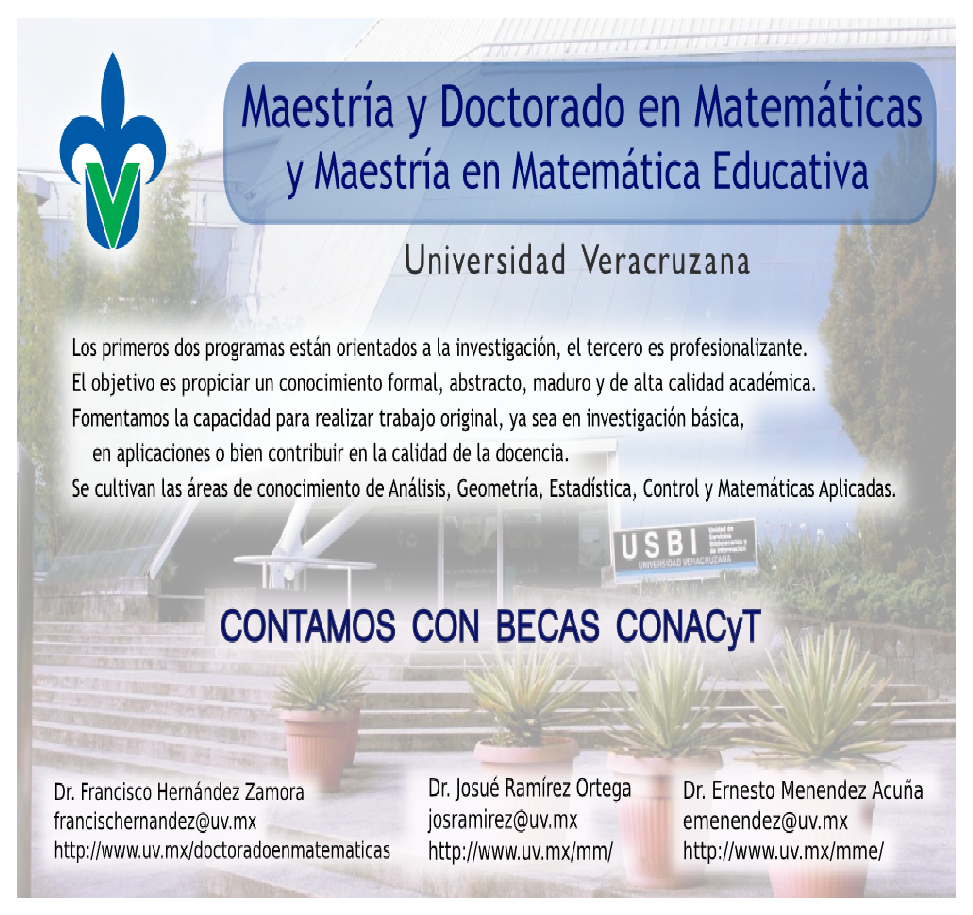
\includegraphics{otros/anuncio_VER.eps}}

\includegraphics[width=8cm,height=11cm]{anuncios/anuncio_UAEH.eps}
\hspace{1cm}
\includegraphics[width=8cm,height=11cm]{otros/POSTER-UANL.eps}
\begin{center}
\includegraphics[width=15cm,height=11cm]{anuncios/anuncio_uv.eps}
%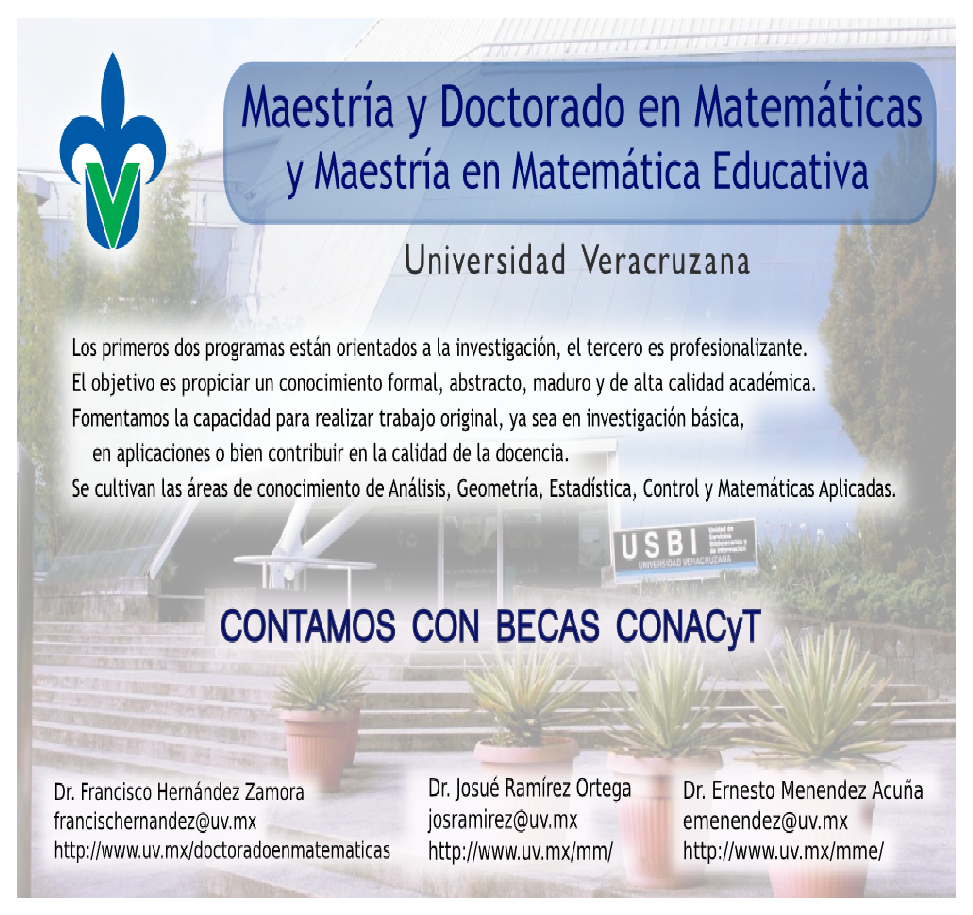
\includegraphics[width=15cm,height=11cm]{otros/anuncio_VER.eps}
\includegraphics[width=17cm]{anuncios/anuncio_memorias.eps}
\end{center}

{\footnotesize
\begin{center}
%\begin{tabular}{|p{50pt}|p{50pt}|p{65pt}|p{65pt}|p{65pt}|p{65pt}|p{65pt}|}
\begin{tabular}{|c|c|c|c|c|c|}
\hline[1pt]
\multicolumn{6}{|c|}{\Large\bfseries Difusi�n de Posgrados p�g. \pageref{reg-671}}\\
\hline
\hline
{\hfill\bfseries Hora\hfill} & {\hfill\bfseries Lunes\hfill} &  {\hfill\bfseries Martes\hfill} & {\hfill\bfseries Mi�rcoles\hfill} & {\hfill\bfseries Jueves\hfill} & {\hfill\bfseries Viernes\hfill} \\
\hline
{\hfill 9:00-9:20 \hfill} &
      &
    &
   {\bfseries \ref{reg-671}} &
        &
      \\
\cline{1-1}\cline{3-6}

{\hfill 9:20-9:40 \hfill} &
      &
    &
   {\bfseries \ref{reg-657}} &
        &
      \\
\cline{1-1}\cline{3-6}

{\hfill 9:40-10:00 \hfill} &
      &
    &
   {\bfseries \ref{reg-859}} &
        &
      \\
\cline{1-1}\cline{3-6}

{\hfill 10:00-10:20 \hfill} &
    Inauguraci�n   &
    &
   {\bfseries \ref{reg-743}} &
    &
     \\
\cline{1-1}\cline{3-6}

{\hfill 10:20-10:40 \hfill} &
    &
    &
    {\bfseries \ref{reg-658}} &
    &
     \\
\cline{1-6}

{\hfill 10:40-11:00 \hfill} &
      &
    &
     {\bfseries \ref{ref-736}} &
      &
     \\
\cline{1-1}\cline{3-6}

{\hfill 11:00-11:30 \hfill} &
     {\bfseries PLENARIA 1 }&
     \multicolumn{4}{|c|} {\bfseries Caf�} \\
\cline{1-6}

{\hfill 11:40-12:00 \hfill} &
     Traslado &
      &
  &
  &
   \\
\cline{1-6}

{\hfill 12:00-12:50 \hfill} &
       &
      &
      &
   &
   \\
\cline{1-6}

{\hfill 12:50-13:00 \hfill} &
     \multicolumn{5}{|c|} {\bfseries Traslado} \\
\cline{1-6}

{\hfill 13:00-13:30 \hfill} &
       &
    {\bfseries PLENARIA  } &
    {\bfseries PLENARIA  } &
   {\bfseries PLENARIA  } &
   {\bfseries PLENARIA  } \\
%\cline{1-2}

{\hfill 13:30-13:50 \hfill} &
      &
    {\bfseries 2  } &
    {\bfseries 3  } &
   {\bfseries 4  } &
   {\bfseries 5  } \\
\cline{1-6}

{\hfill 14:00-16:30 \hfill} &
    \multicolumn{2}{|c|} {\bfseries COMIDA} &
   &
   \multicolumn{2}{|c|} {\bfseries COMIDA} \\
\cline{1-3}\cline{5-6}

{\hfill 16:40-17:00 \hfill} &
       &
    &
     &
     &
     \\
\cline{1-1}\cline{3-3}\cline{5-6}

{\hfill 17:00-17:20 \hfill} &
      &
      &
     &
    &
    \\
\cline{1-1}\cline{3-3}\cline{5-6}

{\hfill 17:20-17:40 \hfill} &
       &
      &
     &
     &
     \\
\cline{1-3}\cline{5-6}

{\hfill 17:40-18:10 \hfill} &
     \multicolumn{2}{|c|} {\bfseries Caf�}&
    {\bfseries Tarde Libre} &
     \multicolumn{2}{|c|} {\bfseries Caf�} \\
\cline{1-3}\cline{5-6}

{\hfill 18:10-18:30 \hfill} &
      &
    &
    &
   {\bfseries PLENARIA  } &
   {\bfseries PLENARIA  } \\
\cline{1-3}

{\hfill 18:30-18:50 \hfill} &
  &
    &
    &
   {\bfseries 8  } &
 {\bfseries 9  } \\
\cline{1-3}\cline{5-6}

{\hfill 18:50-19:00 \hfill} &
    \multicolumn{2}{|c|} {\bfseries Traslado} &
     &
  {\bfseries HOMENAJE} &
  {\bfseries Traslado}  \\
\cline{1-3}\cline{6-6}
{\hfill 19:00-19:50 \hfill} &
 {\bfseries  PLENARIA 6 } &
   {\bfseries  PLENARIA  7} &
       &
   {\bfseries  JORGE} &
   {\bfseries Asamblea } \\
\cline{1-3}
{\hfill 19:50-20:50  \hfill} &
  {\bfseries  HOMENAJE }&
  {\bfseries  HOMENAJE } &
       &
  {\bfseries  IZE}  &
  {\bfseries  General }  \\
  \cline{1-1}\cline{5-6}
{\hfill 20:50-21:00 \hfill} &
 {\bfseries  ERNESTO }  &
   {\bfseries FRANCISCO} &
       &
  &
   {\bfseries Traslado } \\
\cline{1-1}\cline{5-6}
    {\hfill 21:00-21:50  \hfill} &
 {\bfseries  LACOMBA } &
   {\bfseries RAGGI} &
       &
    &
   {\bfseries Clausura}   \\
\cline{1-6}

\hline[1pt]
\multicolumn{6}{|c|}{\large\bfseries Sal�n I9 }\\
\hline
\end{tabular}
\end{center}

}

\begin{multicols}{2}
\raggedcolumns



%%%%%%%%%%%%671%%%%%%%%%%%%
\noindent \ref{reg-671} {\bfseries Maestr�a en Ciencias en Matem�ticas Aplicadas} \\
{\slshape Gamaliel Bl� Gonz�lez} {\footnotesize (CDV, 2Lic)} \\


%%%%%%%%%%%%657%%%%%%%%%%%%
\noindent \ref{reg-657} {\bfseries Posgrado Conjunto en Ciencias Matem�ticas UMSNH-UNAM} \\
{\slshape Adriana Brise�o Ch�vez} {\footnotesize (CDV, Pos)} \\


%%%%%%%%%%%%859%%%%%%%%%%%%
\noindent \ref{reg-859} {\bfseries El Posgrado de Matem�ticas de la UAM-Iztapalapa} \\
{\slshape Jos� Ra�l Montes de Oca Machorro} {\footnotesize (CDV, 2Lic)} \\

\columnbreak

%%%%%%%%%%%%743%%%%%%%%%%%%
\noindent \ref{reg-743} {\bfseries Posgrados en la Facultad de Matem�ticas de la Universidad Aut�noma de Yucat�n} \\
{\slshape Ram\'on Peniche Mena Peniche Mena} {\footnotesize (CDV, 2Lic)} \\


%%%%%%%%%%%%658%%%%%%%%%%%%
\noindent \ref{reg-658} {\bfseries Posgrado en Optimizaci�n en la UAM Azcapotzalco} \\
{\slshape Francisco Javier Zaragoza Mart�nez} {\footnotesize (CDV, 2Lic)} \\


%%%%%%%%%%%%736%%%%%%%%%%%%
\noindent \ref{ref-736} {\bfseries Maestr�a en Estad�stica Aplicada} \\
{\slshape Jos� Eliud Silva Urrutia} {\footnotesize (CDV, 2Lic)} \\

\pagebreak

\end{multicols}
      % 34
{\footnotesize
\begin{center}
%\begin{tabular}{|p{50pt}|p{50pt}|p{65pt}|p{65pt}|p{65pt}|p{65pt}|p{65pt}|}
\begin{tabular}{|c|c|c|c|c|c|}
\hline[1pt]
\multicolumn{6}{|c|}{\Large\bfseries Presentaci�n de Libros p�g. \pageref{reg-540}}\\
\hline
\hline
{\hfill\bfseries Hora\hfill} & {\hfill\bfseries Lunes\hfill} &  {\hfill\bfseries Martes\hfill} & {\hfill\bfseries Mi�rcoles\hfill} & {\hfill\bfseries Jueves\hfill} & {\hfill\bfseries Viernes\hfill} \\
\hline
{\hfill 9:00-9:20 \hfill} &
      &
   {\bfseries \ref{reg-540}} &
   {\bfseries \ref{reg-1371}} &
        &
      \\
\cline{1-1}\cline{3-6}

{\hfill 9:20-9:40 \hfill} &
      &
   {\bfseries \ref{reg-868}} &
   {\bfseries \ref{reg-730}} &
        &
      \\
\cline{1-1}\cline{3-6}

{\hfill 9:40-10:00 \hfill} &
   Inauguraci�n &
   {\bfseries \ref{reg-601}} &
   {\bfseries \ref{reg-380}} &
        &
      \\
\cline{1-1}\cline{3-6}

{\hfill 10:00-10:20 \hfill} &
    &
   {\bfseries \ref{reg-411}} &
   {\bfseries \ref{reg-1109}} &
    &
     \\
\cline{1-1}\cline{3-6}

{\hfill 10:20-10:40 \hfill} &
    &
   {\bfseries \ref{reg-546}} &
   {\bfseries \ref{reg-1769}} &
    &
     \\
\cline{1-6}

{\hfill 10:40-11:00 \hfill} &
      &
    {\bfseries \ref{reg-678}} &
    {\bfseries \ref{reg-418}} &
      &
     \\
\cline{1-1}\cline{3-6}

{\hfill 11:00-11:30 \hfill} &
     {\bfseries PLENARIA 1 }&
     \multicolumn{4}{|c|} {\bfseries Caf�} \\
\cline{1-6}

{\hfill 11:30-11:50 \hfill} &
    Traslado &
    {\bfseries \ref{reg-561}} &
    {\bfseries \ref{reg-1378}} &
  &
   \\
\cline{1-6}

{\hfill 12:00-12:30 \hfill} &
       &
     {\bfseries \ref{reg-386}} &
     {\bfseries \ref{reg-1622}} &
   &
   \\
\cline{1-1}\cline{3-6}

{\hfill 12:30-12:50 \hfill} &
       &
     {\bfseries \ref{reg-608}} &
      &
   &
   \\
\cline{1-6}

{\hfill 12:50-13:00 \hfill} &
     \multicolumn{5}{|c|} {\bfseries Traslado} \\
\cline{1-6}

{\hfill 13:00-13:30 \hfill} &
       &
    {\bfseries PLENARIA  } &
    {\bfseries PLENARIA  } &
   {\bfseries PLENARIA  } &
   {\bfseries PLENARIA  } \\
%\cline{1-2}

{\hfill 13:30-13:50 \hfill} &
      &
    {\bfseries 2  } &
    {\bfseries 3  } &
   {\bfseries 4  } &
   {\bfseries 5  } \\
\cline{1-6}

{\hfill 14:00-16:30 \hfill} &
    \multicolumn{2}{|c|} {\bfseries COMIDA} &
   &
   \multicolumn{2}{|c|} {\bfseries COMIDA} \\
\cline{1-3}\cline{5-6}

{\hfill 16:40-17:00 \hfill} &
       &
   {\bfseries \ref{reg-588}} &
     &
     &
     \\
\cline{1-1}\cline{3-3}\cline{5-6}

{\hfill 17:00-17:20 \hfill} &
      &
     {\bfseries \ref{reg-1745}} &
     &
    &
    \\
\cline{1-1}\cline{3-3}\cline{5-6}

{\hfill 17:20-17:40 \hfill} &
       &
     {\bfseries \ref{reg-1528}} &
     &
     &
     \\
\cline{1-3}\cline{5-6}

{\hfill 17:40-18:10 \hfill} &
     \multicolumn{2}{|c|} {\bfseries Caf�}&
    {\bfseries Tarde Libre} &
     \multicolumn{2}{|c|} {\bfseries Caf�} \\
\cline{1-3}\cline{5-6}

{\hfill 18:10-18:30 \hfill} &
      &
   {\bfseries \ref{reg-580}} &
    &
   {\bfseries PLENARIA  } &
   {\bfseries PLENARIA  } \\
\cline{1-3}

{\hfill 18:30-18:50 \hfill} &
  &
    &
    &
   {\bfseries 8  } &
 {\bfseries 9  } \\
\cline{1-3}\cline{5-6}

{\hfill 18:50-19:00 \hfill} &
    \multicolumn{2}{|c|} {\bfseries Traslado} &
     &
  {\bfseries Traslado} &
    \\
\cline{1-3}\cline{5-5}

{\hfill 19:00-19:50 \hfill} &
 {\bfseries PLENARIA 6 } &
   {\bfseries PLENARIA  7} &
       &
   {\bfseries Asamblea General } &
   {\bfseries Clausura } \\
\cline{1-6}

\hline[1pt]
\multicolumn{6}{|c|}{\large\bfseries Sal�n I9 }\\
\hline
\end{tabular}
\end{center}

}

\begin{multicols}{2}
\raggedcolumns



%%%%%%%%%%%%540%%%%%%%%%%%%
\noindent \ref{reg-540} {\bfseries Introducci�n al �lgebra lineal} \\
{\slshape Carlos Daniel Prado P�rez} {\footnotesize (1Lic)}\\


%%%%%%%%%%%%868%%%%%%%%%%%%
\noindent \ref{reg-868} {\bfseries Introduction to Vassiliev knot invariants} \\
{\slshape Jacob Mostovoy} {\footnotesize (Pos)}\\


%%%%%%%%%%%%601%%%%%%%%%%%%
\noindent \ref{reg-601} {\bfseries �Hacia d�nde reorientar el curriculum de matem�ticas del bachillerato?} \\
{\slshape Cris�logo Dolores Flores} {\footnotesize (Bach)}\\


%%%%%%%%%%%%411%%%%%%%%%%%%
\noindent \ref{reg-411} {\bfseries Teor�a de Conjuntos, Curso intermedio} \\
{\slshape Gabriela Campero Arena} {\footnotesize (2Lic)}\\


%%%%%%%%%%%%546%%%%%%%%%%%%
\noindent \ref{reg-546} {\bfseries Selected Topics on Continuous-Time Controlled Markov Chains and Markov Games} \\
{\slshape Onesimo Hernandez-Lerma} {\footnotesize (Pos)}\\


%%%%%%%%%%%%678%%%%%%%%%%%%
\noindent \ref{reg-678} {\bfseries Ingenier�a de sistemas. Investigaci�n e intervenci�n} \\
{\slshape Bruno C�sar Gonz�lez Fern�ndez} {\footnotesize (Pos)}\\

\columnbreak

%%%%%%%%%%%%561%%%%%%%%%%%%
\noindent \ref{reg-561} {\bfseries Fluid Dynamics, Computational Modeling and Applications} \\
{\slshape Lorenzo H�ctor Ju�rez Valencia} {\footnotesize (Inv)}\\


%%%%%%%%%%%%386%%%%%%%%%%%%
\noindent \ref{reg-386} {\bfseries Presentaci�n del e-Book: M�todos Num�ricos para Ingenier�a} \\
{\slshape Francisco Javier Delgado-Cepeda} {\footnotesize (2Lic)}\\


%%%%%%%%%%%%608%%%%%%%%%%%%
\noindent \ref{reg-608} {\bfseries Mixba�al, Revista Metropolitana de Matem�ticas} \\
{\slshape Joaqu�n Delgado Fern�ndez} {\footnotesize (Pos)}\\


%%%%%%%%%%%%588%%%%%%%%%%%%
\noindent \ref{reg-588} {\bfseries Geometr\'{\i}ia analitica plana} \\
{\slshape Rene Benitez Lopez} {\footnotesize (Bach)}\\


%%%%%%%%%%%%1745%%%%%%%%%%%%
\noindent \ref{reg-1745} {\bfseries Futbol y matematicas.  Juegos para aprender de forma divertida} \\
{\slshape Pablo Rodrigo Zeleny Vazque} {\footnotesize (Prim)}\\


%%%%%%%%%%%%1528%%%%%%%%%%%%
\noindent \ref{reg-1528} {\bfseries aC�rcate. Revista de divulgaci�n de ciencia y tecnolog�a de la UACM} \\
{\slshape Catalina Trevilla Rom�n} {\footnotesize }


%%%%%%%%%%%%580%%%%%%%%%%%%
\noindent \ref{reg-580} {\bfseries Teor�a de Galois, un primer curso} \\
{\slshape Emilio Esteban Lluis Puebla} {\footnotesize (1Lic)}\\


%%%%%%%%%%%%1371%%%%%%%%%%%%
\noindent \ref{reg-1371} {\bfseries Grupos de Difeomorfismos} \\
{\slshape Pablo Su�rez Serrato} {\footnotesize (Pos)}\\


%%%%%%%%%%%%730%%%%%%%%%%%%
\noindent \ref{reg-730} {\bfseries Fundamentos de matem�ticas b�sicas} \\
{\slshape Ernesto �lvarez Gonz�lez} {\footnotesize (Bach)}\\


%%%%%%%%%%%%380%%%%%%%%%%%%
\noindent \ref{reg-380} {\bfseries Matem�ticas III Bajo el enfoque por competencias con estricto apego a la RIEMS} \\
{\slshape Enrique Rivera Castillo} {\footnotesize (Bach)}\\


%%%%%%%%%%%%1109%%%%%%%%%%%%
\noindent \ref{reg-1109} {\bfseries Una introducci�n a la geometr�a hiperb�lica y a los grupos fuchsianos} \\
{\slshape Rogelio Valdez Delgado} {\footnotesize (2Lic)}\\

\columnbreak

%%%%%%%%%%%%1769%%%%%%%%%%%%
\noindent \ref{reg-1769} {\bfseries Ludoteca interactiva de matem�ticas secundaria} \\
{\slshape Gers�n Hern�ndez Mart�nez} {\footnotesize (Sec)}\\


%%%%%%%%%%%%418%%%%%%%%%%%%
\noindent \ref{reg-418} {\bfseries New Foundations in Mathematics: The Geometric Concept of Number} \\
{\slshape Garret Sobczyk} {\footnotesize (2Lic)}\\


%%%%%%%%%%%%1378%%%%%%%%%%%%
\noindent \ref{reg-1378} {\bfseries Uno, dos, tres, \ldots, infinito, \ldots, y m�s all�} \\
{\slshape Alejandro R. Garciadiego Dantan} {\footnotesize (Prim)}\\


%%%%%%%%%%%%1622%%%%%%%%%%%%
\noindent \ref{reg-1622} {\bfseries C�lculo Diferencial. Fundamentos, aplicaciones y notas hist�ricas} \\
{\slshape Antonio Rivera-Figueroa} {\footnotesize (1Lic)}\\



\end{multicols}
      % 35
{\footnotesize
\begin{center}
%\begin{tabular}{|p{50pt}|p{50pt}|p{65pt}|p{65pt}|p{65pt}|p{65pt}|p{65pt}|}
\begin{tabular}{|c|c|c|c|c|c|}
\hline[1pt]
\multicolumn{6}{|c|}{\Large\bfseries De Joven a Joven p�g. \pageref{Joven02}}\\
\hline
\hline
{\hfill\bfseries Hora\hfill} & {\hfill\bfseries Lunes\hfill} &  {\hfill\bfseries Martes\hfill} & {\hfill\bfseries Mi�rcoles\hfill} & {\hfill\bfseries Jueves\hfill} & {\hfill\bfseries Viernes\hfill} \\
\hline
{\hfill 9:00-9:50 \hfill} &   &   &   &   &   \\
\cline{1-1}\cline{3-6}

{\hfill 10:00-10:20 \hfill} &
    Inauguraci�n   &
    &
    &
    &
     \\
\cline{1-1}\cline{3-6}

{\hfill 10:20-10:40 \hfill} &
    &
    &
     &
    &
     \\
\cline{1-6}

{\hfill 10:40-11:00 \hfill} &
     {\bfseries PLENARIA 1 } &
    &
      &
      &
     \\
\cline{1-2}\cline{3-6}

{\hfill \multirow{4}{*}{11:00-12:00} \hfill} &
%{\hfill 11:00-11:20 \hfill} &
%     {\bfseries PLENARIA 1 }&
     {\bfseries \ref{Joven02}},
     {\bfseries \ref{joven04}},
     {\bfseries \ref{joven05}},
     {\bfseries \ref{joven06}},
&
     {\bfseries \ref{joven04}},
     {\bfseries \ref{joven06}},
     {\bfseries \ref{joven07}},
     {\bfseries \ref{joven19}},
&  \multicolumn{3}{|c|} {\bfseries} \\
%\cline{1-1}%\cline{4-6}

%{\hfill 11:20-11:40 \hfill} 
&
     {\bfseries \ref{joven21}},
     {\bfseries \ref{joven07}},
     {\bfseries \ref{joven08}},
     
 &
     {\bfseries \ref{joven13}},
     {\bfseries \ref{joven03}},
     {\bfseries \ref{joven09}},
     {\bfseries \ref{joven10}},
&  \multicolumn{3}{|c|} {\bfseries Caf�} \\
%\cline{4-6}

&
     %{\bfseries \ref{joven13}},
     {\bfseries \ref{joven11}},
     {\bfseries \ref{joven14}},
     {\bfseries \ref{joven15}},
 &
     {\bfseries \ref{joven12}},
     {\bfseries \ref{joven17}},
     {\bfseries \ref{joven18}},\vspace{-6pt}
&  \multicolumn{3}{|c|} {\bfseries} \\
\cline{4-6}

%{\hfill 11:40-12:00 \hfill} 
&
     {\bfseries \ref{joven16}},
     {\bfseries \ref{joven19}}
 &
     {\bfseries \ref{joven20}},
     {\bfseries \ref{joven22}},
     {\bfseries \ref{joven23}}
 & & & \\
\cline{1-6}

{\hfill 12:00-12:50 \hfill} &
       &
      &
      &
   &
   \\
\cline{1-6}

{\hfill 12:50-13:00 \hfill} &
     \multicolumn{5}{|c|} {\bfseries Traslado} \\
\cline{1-6}

{\hfill 13:00-13:30 \hfill} &
       &
    {\bfseries PLENARIA  } &
    {\bfseries PLENARIA  } &
   {\bfseries PLENARIA  } &
   {\bfseries PLENARIA  } \\
%\cline{1-2}

{\hfill 13:30-13:50 \hfill} &
      &
    {\bfseries 2  } &
    {\bfseries 3  } &
   {\bfseries 4  } &
   {\bfseries 5  } \\
\cline{1-6}

{\hfill 14:00-16:30 \hfill} &
    \multicolumn{2}{|c|} {\bfseries COMIDA} &
   &
   \multicolumn{2}{|c|} {\bfseries COMIDA} \\
\cline{1-3}\cline{5-6}

{\hfill 16:40-17:00 \hfill} &
       &
    &
     &
     &
     \\
\cline{1-3}\cline{5-6}

{\hfill 17:00-17:20 \hfill} &
      &
&
     &
    &
    \\
\cline{1-2}\cline{5-6}

{\hfill 17:20-17:40 \hfill} &
       &
      {\bfseries \ref{joven16}},
      {\bfseries \ref{joven01}}
      &
     &
     &
     \\
\cline{1-2}\cline{5-6}

{\hfill 17:40-18:00 \hfill} &
%     \multicolumn{2}{|c|} {\bfseries Caf�}&
\bfseries Caf� &
 &
    {\bfseries Tarde Libre} &
     \multicolumn{2}{|c|} {\bfseries Caf�} \\
\cline{1-3}\cline{5-6}

{\hfill 18:10-18:30 \hfill} &
      &
    &
    &
   {\bfseries PLENARIA  } &
   {\bfseries PLENARIA  } \\
\cline{1-3}

{\hfill 18:30-18:50 \hfill} &
  &
    &
    &
   {\bfseries 8  } &
 {\bfseries 9  } \\
\cline{1-3}\cline{5-6}

{\hfill 18:50-19:00 \hfill} &
    \multicolumn{2}{|c|} {\bfseries Traslado} &
     &
  {\bfseries HOMENAJE} &
  {\bfseries Traslado}  \\
\cline{1-3}\cline{6-6}
{\hfill 19:00-19:50 \hfill} &
 {\bfseries  PLENARIA 6 } &
   {\bfseries  PLENARIA  7} &
       &
   {\bfseries  JORGE} &
   {\bfseries Asamblea } \\
\cline{1-3}
{\hfill 19:50-20:50  \hfill} &
  {\bfseries  HOMENAJE }&
  {\bfseries  HOMENAJE } &
       &
  {\bfseries  IZE}  &
  {\bfseries  General }  \\
  \cline{1-1}\cline{5-6}
{\hfill 20:50-21:00 \hfill} &
 {\bfseries  ERNESTO }  &
   {\bfseries FRANCISCO} &
       &
  &
   {\bfseries Traslado } \\
\cline{1-1}\cline{5-6}
    {\hfill 21:00-21:50  \hfill} &
 {\bfseries  LACOMBA } &
   {\bfseries RAGGI} &
       &
    &
   {\bfseries Clausura}   \\
\cline{1-6}

\hline[1pt]
\multicolumn{6}{|c|}{\large\bfseries Diferentes Escuelas }\\
\hline
\end{tabular}
\end{center}

}

\begin{multicols}{2}
\raggedcolumns


%%%%%%%%%%%%joven02%%%%%%%%%%%%
\noindent \ref{Joven02} {\bfseries Evariste Galois: Un revolucionario, un matem�tico}\\
{\slshape Leonardo Ignacio Mart�nez Sandoval} \\
%{Lugar: \slshape Colegio Victor Frankl (Secundaria)} \\
{Lugar: \slshape Colegio de Bachilleres del Estado de Quer�taro. Plantel 16 - General L�zaro C�rdenas - El Colorado} \\


%%%%%%%%%%%%joven04%%%%%%%%%%%%
\noindent \ref{joven04} {\bfseries Buscando simetr�as (y otras estructuras escondidas)}\\
{\slshape Luis Miguel Garc�a Vel�zquez} \\
{Lugar:\slshape Escuela de Bachilleres ``Salvador Allende'' Plantel Ajuchitl�n (UAQ)} \\
{Lugar:\slshape Escuela de Bachilleres ``Salvador Allende'' Plantel Pedro Escobedo (UAQ)} \\


%%%%%%%%%%%%joven05%%%%%%%%%%%%
\noindent \ref{joven05} {\bfseries C�ctel de acuarelas}\\
{\slshape Susana Pati�o Espinosa} \\
{Lugar: \slshape Escuela de Bachilleres ``Salvador Allende'' Plantel Bicentenario (UAQ)} \\


%%%%%%%%%%%%joven06%%%%%%%%%%%%
\noindent \ref{joven06} {\bfseries El misterio de la casa roja y la gr�fica delatora}\\
{\slshape Gasde Augusto Hunedy L�pez} \\
{Lugar: \slshape CBTIS 118 Corregidora} \\
{Lugar: \slshape CETIS 105 Santa Maria Magdalena} \\

%\columnbreak

%%%%%%%%%%%%joven21%%%%%%%%%%%%
\noindent \ref{joven21} {\bfseries Contando al infinito y mas all�}\\
{\slshape Pedro Franco} \\
{Lugar: \slshape Preparatoria Gran Breta�a} \\


%%%%%%%%%%%%joven07%%%%%%%%%%%%
\noindent \ref{joven07} {\bfseries Una Introducci�n a las Coloraciones en Teor�a de Gr�ficas}\\
{\slshape Denae Ventura} \\
{Lugar: \slshape Colegio de Bachilleres Del Estado de Quer�taro Plantel 1 - Sat�lite} \\
{Lugar: \slshape Colegio de Bachilleres Del Estado de Quer�taro Plantel 3 - Corregidora} \\


%%%%%%%%%%%%joven08%%%%%%%%%%%%
\noindent \ref{joven08} {\bfseries Historia de una batalla naval argumentada matem�ticamente}\\
{\slshape Il�n A. Goldfeder} \\
{Lugar: \slshape Colegio de Bachilleres Del Estado de Quer�taro Plantel 7 - El Marques} \\


%%%%%%%%%%%%joven11%%%%%%%%%%%%
\noindent \ref{joven11} {\bfseries De infinitos a INFINITOS}\\
{\slshape Iv�n Ongay Valverde} \\
{Lugar: \slshape Colegio de Bachilleres Del Estado de Quer�taro Plantel 13 - Epigmenio Gonz�lez} \\

%\columnbreak


%%%%%%%%%%%%joven14%%%%%%%%%%%%
\noindent \ref{joven14} {\bfseries ?`Sabes contar?}\\
{\slshape Juli�n Fres�n} \\
{Lugar: \slshape Colegio de Bachilleres Del Estado de Quer�taro Plantel 19 - Bravo - Corregidora} \\


%%%%%%%%%%%%joven15%%%%%%%%%%%%
\noindent \ref{joven15} {\bfseries ?`D�nde trabajan los matem�ticos?}\\
{\slshape Alma Violeta Garc�a L�pez} \\
{LUgar: \slshape Colegio de Bachilleres Del Estado de Quer�taro Plantel 21 - Arcila, SJR} \\


%%%%%%%%%%%%joven16%%%%%%%%%%%%
\noindent \ref{joven16} {\bfseries !`A jugar!}\\
{\slshape Luis Antonio Ruiz L�pez} \\
{Lugar: \slshape CECYTEQ corregidora} \\
{Lugar: \slshape Colegio MAXEI (Secundaria)} \\


%%%%%%%%%%%%joven19%%%%%%%%%%%%
\noindent \ref{joven19} {\bfseries Lenguajes y c�digos}\\
{\slshape Jos� Pablo del Cueto Navarro} \\
{Lugar: \slshape CONALEP Quer�taro} \\
{Lugar: \slshape CONALEP El Marqu�s} \\


%%%%%%%%%%%%joven13%%%%%%%%%%%%
\noindent \ref{joven13} {\bfseries ?`Cu�ntas dimensiones?}\\
{\slshape Rodrigo Jes�s Hern�ndez Guti�rrez} \\
%{Lugar: \slshape Colegio de Bachilleres Del Estado de Quer�taro Plantel 16 - General Lazaro Cardenas - El Colorado} \\
{Lugar: \slshape Colegio de Bachilleres Del Estado de Quer�taro Plantel 17 - Constituci�n de 1917} \\


%%%%%%%%%%%%joven03%%%%%%%%%%%%
\noindent \ref{joven03} {\bfseries Lo raro del infinito y otras curiosidades en mate}\\
{\slshape Manuel Alejandro Ju�rez Camacho} \\
{Lugar: \slshape Escuela de Bachilleres ``Salvador Allende'' Plantel San Juan del R�o (UAQ)} \\


%%%%%%%%%%%%joven09%%%%%%%%%%%%
\noindent \ref{joven09} {\bfseries Las matem�ticas en el reloj y los mensajes secretos}\\
{\slshape Anayanzi Delia Mart�nez Hern�ndez} \\
{Lugar: \slshape Colegio de Bachilleres Del Estado de Quer�taro Plantel 8 - Azteca} \\

%\columnbreak

%%%%%%%%%%%%joven10%%%%%%%%%%%%
\noindent \ref{joven10} {\bfseries Matem�ticas, recursi�n y el fin del mundo}\\
{\slshape Micael Toledo} \\
{Lugar: \slshape Colegio de Bachilleres Del Estado de Quer�taro Plantel 9 - Santa Rosa Jauregu�} \\


%%%%%%%%%%%%joven12%%%%%%%%%%%%
\noindent \ref{joven12} {\bfseries Conociendo a los conjuntos fractales}\\
{\slshape Mar�a Cristina Cid Zepeda} \\
{Lugar: \slshape Colegio de Bachilleres Del Estado de Quer�taro Plantel 15 - Chichimequillas} \\


%%%%%%%%%%%%joven17%%%%%%%%%%%%
\noindent \ref{joven17} {\bfseries Las paradojas del infinito}\\
{\slshape Erick Garc�a Ram�rez} \\
{Lugar: \slshape CECYTEQ Pedro Escobedo} \\


%%%%%%%%%%%%joven18%%%%%%%%%%%%
\noindent \ref{joven18} {\bfseries ?`C�mo enviar informaci�n confidencial?}\\
{\slshape Ana Victoria Ponce Bobadilla} \\
{Lugar: \slshape CECYTEQ SJR} \\


%%%%%%%%%%%%joven20%%%%%%%%%%%%
\noindent \ref{joven20} {\bfseries Una definici�n ``diferente'' de una gr�fica}\\
{\slshape Alejandra Ramos Rivera} \\
{Lugar: \slshape CONALEP SJR} \\


%%%%%%%%%%%%joven22%%%%%%%%%%%%
\noindent \ref{joven22} {\bfseries Jugando Canicas en el Espacio}\\
{\slshape Alma Roc�o Sagaceta Mej�a} \\
{Lugar: \slshape Escuela de Bachilleres ``Salvador Allende'' Plantel Norte (UAQ)} \\


%%%%%%%%%%%%joven23%%%%%%%%%%%%
\noindent \ref{joven23} {\bfseries ?`Un mono puede escribir las obras completas de Shakespeare?}\\
{\slshape Jes�s Daniel Arroyo Reli�n} \\
{Lugar: \slshape CECYTEQ cerrito colorado} \\


%%%%%%%%%%%%joven01%%%%%%%%%%%%
\noindent \ref{joven01} {\bfseries Curiosidades de n�meros primos}\\
{\slshape Leonardo Ignacio Mart�nez Sandoval} \\
{Lugar: \slshape Escuela de Bachilleres ``Salvador Allende'' Plantel Sur (UAQ)} \\



\end{multicols}

%%%%%%%%%%%%%%%%%%%%%%%%%%%%%%%%%%%%%%%%%%%%%%%%%%%%%%%%%%%%%5

%\newpage

{\footnotesize
\begin{center}
%\begin{tabular}{|p{50pt}|p{50pt}|p{65pt}|p{65pt}|p{65pt}|p{65pt}|p{65pt}|}
\begin{tabular}{|c|c|c|c|c|c|c|c|}
\hline[1pt]
\multicolumn{8}{|c|}{\Large\bfseries De Joven a Joven p�g. \pageref{reg-joven29}}\\
\hline
\hline
{\hfill\bfseries Hora\hfill} & \multicolumn{2}{|c|}{\bfseries Lunes} &  \multicolumn{2}{|c|}{\bfseries Martes} & {\hfill\bfseries Mi�rcoles\hfill} & {\hfill\bfseries Jueves\hfill} & {\hfill\bfseries Viernes\hfill} \\
\hline
{\hfill 9:00-9:30 \hfill} & \multicolumn{2}{|c|}{\multirow{2}{*}{\bfseries \ref{reg-joven29}}} & \multicolumn{2}{|c|}{\multirow{2}{*}{{\bfseries \ref{joven27}}, {\bfseries \ref{joven37}}}}  &   &   &   \\
\cline{1-1}\cline{6-8}
{\hfill 9:30-10:00 \hfill} & \multicolumn{2}{|c|}{} & \multicolumn{2}{|c|}{}  &   &   &   \\
\hline
{\hfill 10:00-10:30 \hfill} &
\multirow{2}{*}{{\bfseries \ref{joven34}}, {\bfseries \ref{joven25}}} &  &
\multirow{2}{*}{{\bfseries \ref{joven28}}, {\bfseries \ref{joven35}}}  &   &   &  & \\
\cline{1-1}\cline{3-3}\cline{5-8}
{\hfill 10:30-11:00 \hfill} &  & \multirow{2}{*}{\bfseries \ref{joven38}}  & & \multirow{2}{*}{\bfseries \ref{joven39}}  &   &   &   \\
\cline{1-2}\cline{4-4}\cline{6-8}
{\hfill 11:00-11:30 \hfill} & \multirow{2}{*}{{\bfseries \ref{reg-joven30}}, {\bfseries \ref{reg-joven24}}} & & \multirow{2}{*}{{\bfseries \ref{reg-joven24}}, {\bfseries \ref{joven31}}} & & \multicolumn{3}{|c|}{\bfseries Caf�}   \\
\cline{1-1}\cline{3-3}\cline{5-8}
{\hfill 11:30-12:00 \hfill} &  &  &   &   &   &  & \\
\hline
{\hfill 12:00-12:30 \hfill} & \multicolumn{2}{|c|}{}  & \multicolumn{2}{|c|}{}  &   &   &   \\
\cline{1-1}\cline{6-8}
{\hfill 12:30-12:50 \hfill} & \multicolumn{2}{|c|}{{\bfseries \ref{joven33}}, {\bfseries \ref{joven26}}}  &  \multicolumn{2}{|c|}{{\bfseries \ref{joven32}}, {\bfseries \ref{joven36}}} &   &   &   \\
\cline{1-1}\cline{6-8}

{\hfill 12:50-13:00 \hfill} & \multicolumn{2}{|c|}{} & \multicolumn{2}{|c|}{} &
     \multicolumn{3}{|c|} {\bfseries Traslado} \\
\hline

\multirow{2}{*}{\hfill 13:00-13:50 \hfill} &
\multicolumn{2}{|c|}{}       &
\multicolumn{2}{|c|}{\bfseries PLENARIA  } &
    {\bfseries PLENARIA  } &
   {\bfseries PLENARIA  } &
   {\bfseries PLENARIA  } \\
%\cline{1-2}

 &
\multicolumn{2}{|c|}{}      &
\multicolumn{2}{|c|}{\bfseries 2  } &
    {\bfseries 3  } &
   {\bfseries 4  } &
   {\bfseries 5  } \\
\hline

{\hfill 14:00-16:30 \hfill} &
    \multicolumn{4}{|c|} {\bfseries COMIDA} &
   &
   \multicolumn{2}{|c|} {\bfseries COMIDA} \\
\hline

{\hfill 16:40-17:00 \hfill} &
\multicolumn{2}{|c|}{}       &
\multicolumn{2}{|c|}{}    &
     &
     &
     \\
\cline{1-5}\cline{7-8}

{\hfill 17:00-17:20 \hfill} &
\multicolumn{2}{|c|}{}      &
\multicolumn{2}{|c|}{}      &
     &
    &
    \\
\cline{1-5}\cline{7-8}

{\hfill 17:20-17:40 \hfill} &
\multicolumn{2}{|c|}{}       &
\multicolumn{2}{|c|}{}      &
     &
     &
     \\
\cline{1-5}\cline{7-8}

{\hfill 17:40-18:10 \hfill} &
     \multicolumn{4}{|c|} {\bfseries Caf�}&
    {\bfseries Tarde Libre} &
     \multicolumn{2}{|c|} {\bfseries Caf�} \\
\cline{1-5}\cline{7-8}

{\hfill 18:10-18:30 \hfill} &
\multicolumn{2}{|c|}{}      &
\multicolumn{2}{|c|}{}   &
    &
   {\bfseries PLENARIA  } &
   {\bfseries PLENARIA  } \\
\cline{1-5}

{\hfill 18:30-18:50 \hfill} &
\multicolumn{2}{|c|}{}  &
\multicolumn{2}{|c|}{}  &
    &
   {\bfseries 8  } &
 {\bfseries 9  } \\
\cline{1-5}\cline{7-8}

{\hfill 18:50-19:00 \hfill} &
    \multicolumn{4}{|c|} {\bfseries Traslado} &
     &
  {\bfseries HOMENAJE} &
  {\bfseries Traslado}  \\
\cline{1-5}\cline{8-8}
{\hfill 19:00-19:50 \hfill} &
   \multicolumn{2}{|c|}{\bfseries  PLENARIA 6 } &
    \multicolumn{2}{|c|}  {\bfseries  PLENARIA  7} &
       &
   {\bfseries  JORGE} &
   {\bfseries Asamblea } \\
\cline{1-5	}
{\hfill 19:50-20:50  \hfill} &
  \multicolumn{2}{|c|} {\bfseries  HOMENAJE }&
  \multicolumn{2}{|c|} {\bfseries  HOMENAJE } &
       &
  {\bfseries  IZE}  &
  {\bfseries  General }  \\
  \cline{1-1}\cline{7-8}
{\hfill 20:50-21:00 \hfill} &
  \multicolumn{2}{|c|}{\bfseries  ERNESTO }  &
  \multicolumn{2}{|c|}  {\bfseries FRANCISCO} &
       &
  &
   {\bfseries Traslado } \\
\cline{1-1}\cline{7-8}
    {\hfill 21:00-21:50  \hfill} &
 \multicolumn{2}{|c|} {\bfseries  LACOMBA } &
 \multicolumn{2}{|c|}   {\bfseries RAGGI} &
       &
    &
   {\bfseries Clausura}   \\
\cline{1-6}

\hline[1pt]
\multicolumn{8}{|c|}{\large\bfseries Diferentes Escuelas }\\
\hline
\end{tabular}
\end{center}

}



\begin{multicols}{2}
\raggedcolumns



%%%%%%%%%%%%joven29%%%%%%%%%%%%
\noindent \ref{reg-joven29} {\bfseries Las matem�ticas en todos lados}\\
{\slshape Giovana Ortigoza �lvarez}\\
{Lugar: \slshape Colegio Centro Uni�n, campus S.J.R.} \\


%%%%%%%%%%%%joven34%%%%%%%%%%%%
\noindent \ref{joven34} {\bfseries Soluciones del cubo  un m�todo sencillo para solucionar el cubo de rubik}\\
{\slshape Luis Fernando Rosas Moncada}\\
{Lugar: \slshape Colegio de Bachilleres del Estado de Quer�taro COBAQ 13} \\


%%%%%%%%%%%%joven25%%%%%%%%%%%%
\noindent \ref{joven25} {\bfseries Una Introducci�n a las Coloraciones en Teor�a de Gr�ficas}\\
{\slshape Denae Ventura}\\
{Lugar: \slshape Escuela preparatoria ``Salvador Allende'' Plantel  Sur} \\


%%%%%%%%%%%%joven38%%%%%%%%%%%%
\noindent \ref{joven38} {\bfseries Matem�ticas, Literatura e Historia}\\
{\slshape Norma Ang�lica Rodr�guez Guzm�n}\\
{Lugar: \slshape Esc. Sec. Gral. No. 5 ``Daniel Ortiz Esquivel''} \\


%%%%%%%%%%%%joven30%%%%%%%%%%%%
\noindent \ref{reg-joven30} {\bfseries El quehacer de un matem�tico}\\
{\slshape Giovana Ortigoza �lvarez}\\
{Lugar: \slshape Escuela de Bachilleres ``Salvador Allende'' Plantel San Juan del R�o } \\


%%%%%%%%%%%%joven24%%%%%%%%%%%%
\noindent \ref{reg-joven24} {\bfseries Cuerpos de ancho constante}\\
{\slshape Antonio Rosales Rivera}\\
{Lugar: \slshape Centro de Estudios Tecnol�gicos Industrial y de Servicios CETIS 105} \\
{Lugar: \slshape Secundaria Secundar�a Federal No. 4} \\


%%%%%%%%%%%%joven33%%%%%%%%%%%%
\noindent \ref{joven33} {\bfseries Ley de Snell (Matem�tica  Aplicada)}\\
{\slshape Saydeth Lili Ledesma Molinero}\\
{Lugar: \slshape Colegio de Bachilleres del Estado de Quer�taro COBAQ 14} \\


%%%%%%%%%%%%joven26%%%%%%%%%%%%
\noindent \ref{joven26} {\bfseries Las matem�ticas no siempre son aburridas}\\
{\slshape Marco Antonio Rojas Tapia}\\
{Lugar: \slshape Instituto Queretano San Javier} \\


%%%%%%%%%%%%joven27%%%%%%%%%%%%
\noindent \ref{joven27} {\bfseries El N�mero de Oro; Phi; la Divina Proporci�n}\\
{\slshape H�ctor Daniel Ba�os Cervantes}\\
{Lugar: \slshape Colegio Nuevo Continente} \\


%%%%%%%%%%%%joven37%%%%%%%%%%%%
\noindent \ref{joven37} {\bfseries Paradojas y Sofismas en Matem�ticas}\\
{\slshape Iv�n Gonz�lez Garc�a}\\
{Lugar: \slshape Secundaria General No. 1} \\

%\pagebreak

%%%%%%%%%%%%joven28%%%%%%%%%%%%
\noindent \ref{joven28} {\bfseries Una visi�n estad�stica de los estudios de opini�n}\\
{\slshape Sara Silva Hern�ndez}\\
{Lugar: \slshape Secundaria General No. 1} \\


%%%%%%%%%%%%joven35%%%%%%%%%%%%
\noindent \ref{joven35} {\bfseries El juego del 15 - 14 de Sam Loyd}\\
{\slshape Pablo Luis Pe�a D�az}\\
{Lugar: \slshape Colegio de Bachilleres del Estado de Quer�taro COBAQ 17} \\


%%%%%%%%%%%%joven39%%%%%%%%%%%%
\noindent \ref{joven39} {\bfseries Descartes, ecuaciones, regla y comp�s}\\
{\slshape Norma Ang�lica Rodr�guez Guzm�n}\\
{Lugar: \slshape Esc. Sec. Gral. No. 5 ``Daniel Ortiz Esquivel''} \\


%%%%%%%%%%%%joven31%%%%%%%%%%%%
\noindent \ref{joven31} {\bfseries Matem�tica l�dica ``El cubo de Rubik''}\\
{\slshape Antonio de Jes�s Torres Hern�ndez}\\
{Lugar: \slshape Escuela preparatoria ``Salvador Allende'' Plantel  Sur} \\


%%%%%%%%%%%%joven32%%%%%%%%%%%%
\noindent \ref{joven32} {\bfseries Algo m�s que aritm�tica}\\
{\slshape Edgar Gonz�lez Arreola}\\
{Lugar: \slshape Escuela preparatoria ``Salvador Allende'' Plantel Norte} \\


%%%%%%%%%%%%joven36%%%%%%%%%%%%
\noindent \ref{joven36} {\bfseries A poco, ?`ah� tambi�n...  hay matem�ticas?}\\
{\slshape Rita Ochoa Cruz}\\
{Lugar: \slshape Colegio de Bachilleres Del Estado de Quer�taro Plantel 8 - Azteca} \\



\end{multicols}
 % 36
\chapter*{�reas}
\addcontentsline{toc}{section}{\'Areas}
{\footnotesize
\begin{center}
%\begin{tabular}{|p{50pt}|p{50pt}|p{65pt}|p{65pt}|p{65pt}|p{65pt}|p{65pt}|}
\begin{tabular}{|c|c|c|c|c|c|}
\hline[1pt]
\multicolumn{6}{|c|}{\Large\bfseries �lgebra Sal�n 1 p�g. \pageref{reg-1075}}\\
\hline
\hline
{\hfill\bfseries Hora\hfill} & {\hfill\bfseries Lunes\hfill}&  {\hfill\bfseries Martes\hfill} & {\hfill\bfseries Mi�rcoles\hfill} & {\hfill\bfseries Jueves\hfill} & {\hfill\bfseries Viernes\hfill} \\
\hline
{\hfill 9:00-9:50 \hfill} &
      &
    \ref{reg-1224} &
  {\bfseries \ref{reg-346}} &
  {\bfseries  \ref{reg-321}}  &
     \\
\cline{1-1}\cline{3-6}
{\hfill 10:00-10:20 \hfill} &
     Inauguraci�n &
     &
     \ref{reg-707} &
    \ref{reg-837} &
    \\
\cline{1-1}\cline{4-6}
{\hfill 10:20-10:40 \hfill} &
      &
   {\bfseries \ref{reg-490}} &
     \ref{reg-510} &
    \ref{reg-965} &
     \\
\cline{1-2}\cline{4-6}
{\hfill 10:40-11:00 \hfill} &
     {\bfseries PLENARIA  } &
     &
   \ref{reg-1684}   &
     &
    \\
\cline{1-1}\cline{3-6}
{\hfill 11:00-11:30 \hfill} &
     {\bfseries  1 }&
     \multicolumn{4}{|c|} {\bfseries Caf�} \\
\cline{1-6}
{\hfill 11:40-12:00 \hfill} &
     Traslado &
    \ref{reg-1460}  &
 &
 &
  \\
\cline{1-6}
{\hfill 12:00-12:50 \hfill} &
   {\bfseries  \ref{reg-1075} } &
    \ref{reg-1282} &
   {\bfseries  \ref{reg-423} }&
   {\bfseries \ref{reg-375}} &
  \\
\cline{1-6}
{\hfill 12:50-13:00 \hfill} &
     \multicolumn{5}{|c|} {\bfseries Traslado} \\
\cline{1-6}
{\hfill 13:00-13:30 \hfill} &
     \ref{reg-1168}  &
    {\bfseries PLENARIA  } &
    {\bfseries PLENARIA  } &
   {\bfseries PLENARIA  } &
   {\bfseries PLENARIA  } \\
\cline{1-2}
{\hfill 13:30-13:50 \hfill} &
    \ref{reg-247}  &
    {\bfseries 2  } &
    {\bfseries 3  } &
   {\bfseries 4  } &
   {\bfseries 5  } \\
\cline{1-6}
{\hfill 14:00-16:30 \hfill} &
    \multicolumn{2}{|c|} {\bfseries COMIDA} &
   &
   \multicolumn{2}{|c|} {\bfseries COMIDA} \\
\cline{1-3}\cline{5-6}
{\hfill 16:40-17:00 \hfill} &
       &
     &
     &
     &
     \\
\cline{1-1}\cline{6-6}
{\hfill 17:00-17:20 \hfill} &
  {\bfseries  \ref{reg-410} }  &
    \ref{reg-345}  &
     &
   &
    \\
\cline{1-1}\cline{6-6}
{\hfill 17:20-17:40 \hfill} &
       &
     &
     &
     &
     \\
\cline{1-3}\cline{5-6}
{\hfill 17:40-18:10 \hfill} &
     \multicolumn{2}{|c|} {\bfseries Caf�}&
    {\bfseries Tarde Libre} &
     \multicolumn{2}{|c|} {\bfseries Caf�} \\
\cline{1-3}\cline{5-6}
{\hfill 18:10-18:30 \hfill} &
     \ref{reg-400} &
    \ref{reg-283} &
    &
   {\bfseries PLENARIA  } &
   {\bfseries PLENARIA  } \\
\cline{1-3}
{\hfill 18:30-18:50 \hfill} &
       &
    \ref{reg-285} &
    &
   {\bfseries 8  } &
   {\bfseries 9  } \\
\cline{1-3}\cline{5-6}
{\hfill 18:50-19:00 \hfill} &
    \multicolumn{2}{|c|} {\bfseries Traslado} &
     &
  {\bfseries HOMENAJE} &
  {\bfseries Traslado}  \\
\cline{1-3}\cline{6-6}
{\hfill 19:00-19:50 \hfill} &
 {\bfseries  PLENARIA 6 } &
   {\bfseries  PLENARIA  7} &
       &
   {\bfseries  JORGE} &
   {\bfseries Asamblea } \\
\cline{1-3}
{\hfill 19:50-20:50  \hfill} &
  {\bfseries  HOMENAJE }&
  {\bfseries  HOMENAJE } &
       &
  {\bfseries  IZE}  &
  {\bfseries  General }  \\
  \cline{1-1}\cline{5-6}
{\hfill 20:50-21:00 \hfill} &
 {\bfseries  ERNESTO }  &
   {\bfseries FRANCISCO} &
       &
  &
   {\bfseries Traslado } \\
\cline{1-1}\cline{5-6}
    {\hfill 21:00-21:50  \hfill} &
 {\bfseries  LACOMBA } &
   {\bfseries RAGGI} &
       &
    &
   {\bfseries Clausura}   \\
\cline{1-6}
\hline[1pt]
\multicolumn{6}{|c|}{\large\bfseries Sal�n  C1}\\
\hline
\end{tabular}
\end{center}

}

\begin{multicols}{2}
\raggedcolumns

%%%%%%%%%%1075%%%%%%%%%%%
\noindent  \ref{reg-1075}  {\bfseries La versi�n categ�rica del �lgebra universal}\\
{\slshape  Francisco  Marmolejo (Invitado)} {\footnotesize (CDV, 2Lic)}\\

%%%%%%%%%%1168%%%%%%%%%%%
\noindent  \ref{reg-1168}  {\bfseries Otra caracterizaci�n de los grupos c�clicos finitos}\\
{\slshape  Juan  Morales Rodr�guez} {\footnotesize (CDV, 2Lic)}\\

%%%%%%%%%%247%%%%%%%%%%%
\noindent  \ref{reg-247}  {\bfseries On the union of increasing chains of torsion-free modules}\\
{\slshape  Jorge Eduardo Mac�as D�az} {\footnotesize (RI, Pos)}\\

%%%%%%%%%%410%%%%%%%%%%%
\noindent  \ref{reg-410}  {\bfseries Combinatoria y representaciones del grupo sim�trico}\\
{\slshape  Ernesto  Vallejo Ruiz (Invitado)} {\footnotesize (CDV, 2Lic)}\\\\

%%%%%%%%%%591%%%%%%%%%%%
%\noindent  \ref{reg-591}  {\bfseries La conjetura finitista: Una conjetura Homol�gica}\\
%{\slshape  Octavio  Mendoza Hern�ndez (Invitado)} {\footnotesize (CDV, Pos)}\\

%%%%%%%%%%400%%%%%%%%%%%
\noindent  \ref{reg-400}  {\bfseries Polinomios c�bicos de permutaci�n autoinvertibles sobre $\boldsymbol{\mathbb{Z}_{p^n}}$ con $\boldsymbol{p>7}$ primo}\\
{\slshape  Carlos Jacob Rubio Barrios} {\footnotesize (RI, 2Lic)}\\

%%%%%%%%%%1224%%%%%%%%%%%
\noindent  \ref{reg-1224}  {\bfseries Clases de M�dulos, la visi�n de Francisco Raggi}\\
{\slshape  Carlos Jos� Signoret} {\footnotesize (CPI, Pos)}\\

%%%%%%%%%%490%%%%%%%%%%%
\noindent  \ref{reg-490}  {\bfseries Ret�culas de Prerradicales}\\
{\slshape  Rogelio  Fern�ndez-Alonso Gonz�lez (Invitado)} {\footnotesize (CDV, 2Lic)}\\

%%%%%%%%%%1460%%%%%%%%%%%
\noindent  \ref{reg-1460}  {\bfseries Algunos aspectos reticulares del conjunto de derivadas en el marco R-tors}\\
{\slshape  Luis �ngel Zald�var Corichi} {\footnotesize (RI, Inv)}\\

%%%%%%%%%%1282%%%%%%%%%%%
\noindent  \ref{reg-1282}  {\bfseries Measuring modules: alternative perspectives in module theory}\\
{\slshape  Sergio Roberto L�pez Permouth} {\footnotesize (CI, Inv)}\\

%%%%%%%%%%345%%%%%%%%%%%
\noindent  \ref{reg-345}  {\bfseries Dimensi�n de Krull y Dimensi�n Cl�sica de Krull de M�dulos}\\
{\slshape  Jaime  Castro P�rez} {\footnotesize (CI, Inv)}\\

%%%%%%%%%%283%%%%%%%%%%%
\noindent  \ref{reg-283}  {\bfseries Anillos para los  cuales la ret�cula de teor�as de torsi�n hereditarias y la ret�cula de clases naturales son isomorfas}\\
{\slshape  Iv�n Fernando Vilchis Montalvo} {\footnotesize (RI, Inv)}\\

%%%%%%%%%%285%%%%%%%%%%%
\noindent  \ref{reg-285}  {\bfseries Acerca de anillos artinianos de ideales principales}\\
{\slshape  C�sar Cejudo Castilla} {\footnotesize (RI, Inv)}\\

%%%%%%%%%%346%%%%%%%%%%%
\noindent  \ref{reg-346}  {\bfseries Cuando Sherlock Holmes usa Calvin Klein: deduciendo grupos por sus marcas}\\
{\slshape  Luis  Valero Elizondo (Invitado)} {\footnotesize (CDV, 2Lic)}\\

%%%%%%%%%%707%%%%%%%%%%%
\noindent  \ref{reg-707}  {\bfseries La funci�n zeta del anillo de Burnside del grupo alternante A4}\\
{\slshape  David  Villa Hern�ndez} {\footnotesize (RI, Pos)}\\

%%%%%%%%%%510%%%%%%%%%%%
\noindent  \ref{reg-510}  {\bfseries Una generalizaci�n a la categor�a de biconjuntos}\\
{\slshape  Jes�s Tadeo Ibarra Tacho} {\footnotesize (CPI, Pos)}\\

%%%%%%%%%%1684%%%%%%%%%%%
\noindent  \ref{reg-1684}  {\bfseries Teor�a de inclinaci�n en categor�as de funtores}\\
{\slshape  Mart\'in  Ort\'iz Morales} {\footnotesize (RT, Pos)}\\

%%%%%%%%%%423%%%%%%%%%%%
\noindent  \ref{reg-423}  {\bfseries Aplicaciones de la forma normal de Smith de una matr\'iz entera}\\
{\slshape  Rafael Heraclio Villarreal Rodr�guez (Invitado)} {\footnotesize (CDV, 2Lic)}\\

%%%%%%%%%%321%%%%%%%%%%%
\noindent  \ref{reg-321}  {\bfseries Series formales sobre gr\'aficas orientadas finitas}\\
{\slshape  Raymundo  Bautista Ramos (Invitado)} {\footnotesize (CDV, 2Lic)}\\

%%%%%%%%%%837%%%%%%%%%%%
\noindent  \ref{reg-837}  {\bfseries Operadores V�rtice y �lgebras de Lie Afines}\\
{\slshape  Jos� �ngel Espinoza Arce} {\footnotesize (CPI, 2Lic)}\\

%%%%%%%%%%965%%%%%%%%%%%
\noindent  \ref{reg-965}  {\bfseries Sobre el orden de polinomios de permutaci�n}\\
{\slshape  Jos� Antonio Sozaya Chan} {\footnotesize (RI, 2Lic)}\\

%%%%%%%%%%375%%%%%%%%%%%
\noindent  \ref{reg-375}  {\bfseries \'Algebra Conmutativa y Teor\'\i a de C\'odigos}\\
{\slshape  Horacio  Tapia-Recillas (Invitado)} {\footnotesize (CDV, 2Lic)}\\


\end{multicols}

{\footnotesize
\begin{center}
%\begin{tabular}{|p{50pt}|p{50pt}|p{65pt}|p{65pt}|p{65pt}|p{65pt}|p{65pt}|}
\begin{tabular}{|c|c|c|c|c|c|}
\hline[1pt]
\multicolumn{6}{|c|}{\Large\bfseries �lgebra Sal�n 2  p�g. \pageref{reg-1243}}\\
\hline
\hline
{\hfill\bfseries Hora\hfill} & {\hfill\bfseries Lunes\hfill}&  {\hfill\bfseries Martes\hfill} & {\hfill\bfseries Mi�rcoles\hfill} & {\hfill\bfseries Jueves\hfill} & {\hfill\bfseries Viernes\hfill} \\
\hline
{\hfill 9:00-9:50 \hfill} &
      &
    &
  \ref{reg-1391} &
    \ref{reg-1704}  &
     \\
\cline{1-1}\cline{3-6}
{\hfill 10:00-10:20 \hfill} &
     Inauguraci�n &
     &
 &
     &
    \\
\cline{1-1}\cline{3-3}\cline{6-6}
{\hfill 10:20-10:40 \hfill} &
      &
    &
     \ref{reg-870} &
    \ref{reg-843} &
     \\
\cline{1-3}\cline{6-6}
{\hfill 10:40-11:00 \hfill} &
     {\bfseries PLENARIA } &
     &
      &
     &
    \\
\cline{1-1}\cline{3-6}
{\hfill 11:00-11:30 \hfill} &
     {\bfseries  1 }&
     \multicolumn{4}{|c|} {\bfseries Caf�} \\
\cline{1-6}
{\hfill 11:40-12:00 \hfill} &
     Traslado &
    \ref{reg-496}  &
&
 &
  \\
\cline{1-6}
{\hfill 12:00-12:50 \hfill} &
     \ref{reg-1243}  &
     &
     \ref{reg-1161} &
    \ref{reg-443} &
  \\
\cline{1-6}
{\hfill 12:50-13:00 \hfill} &
     \multicolumn{5}{|c|} {\bfseries Traslado} \\
\cline{1-6}
{\hfill 13:00-13:30 \hfill} &
     \ref{reg-800}  &
    {\bfseries PLENARIA  } &
    {\bfseries PLENARIA  } &
   {\bfseries PLENARIA  } &
   {\bfseries PLENARIA  } \\
\cline{1-1}
{\hfill 13:30-13:50 \hfill} &
      &
    {\bfseries 2  } &
    {\bfseries 3  } &
   {\bfseries 4  } &
   {\bfseries 5  } \\
\cline{1-6}
{\hfill 14:00-16:30 \hfill} &
    \multicolumn{2}{|c|} {\bfseries COMIDA} &
   &
   \multicolumn{2}{|c|} {\bfseries COMIDA} \\
\cline{1-3}\cline{5-6}
{\hfill 16:40-17:00 \hfill} &
    \ref{reg-948}   &
     &
     &
     &
     \\
\cline{1-3}\cline{6-6}
{\hfill 17:00-17:20 \hfill} &
    \ref{reg-660}  &
      &
     &
    \ref{reg-1813} &
    \\
\cline{1-3}\cline{6-6}
{\hfill 17:20-17:40 \hfill} &
       \ref{reg-814}&
     &
     &
     &
     \\
\cline{1-3}\cline{5-6}
{\hfill 17:40-18:10 \hfill} &
     \multicolumn{2}{|c|} {\bfseries Caf�}&
    {\bfseries Tarde Libre} &
     \multicolumn{2}{|c|} {\bfseries Caf�} \\
\cline{1-3}\cline{5-6}
{\hfill 18:10-18:30 \hfill} &
     \ref{reg-815} &
    \ref{reg-1472} &
    &
   {\bfseries PLENARIA  } &
   {\bfseries PLENARIA  } \\
\cline{1-3}
{\hfill 18:30-18:50 \hfill} &
       &
    \ref{reg-1455} &
    &
   {\bfseries 8  } &
   {\bfseries 9  } \\
\cline{1-3}\cline{5-6}
{\hfill 18:50-19:00 \hfill} &
    \multicolumn{2}{|c|} {\bfseries Traslado} &
     &
  {\bfseries HOMENAJE} &
  {\bfseries Traslado}  \\
\cline{1-3}\cline{6-6}
{\hfill 19:00-19:50 \hfill} &
 {\bfseries  PLENARIA 6 } &
   {\bfseries  PLENARIA  7} &
       &
   {\bfseries  JORGE} &
   {\bfseries Asamblea } \\
\cline{1-3}
{\hfill 19:50-20:50  \hfill} &
  {\bfseries  HOMENAJE }&
  {\bfseries  HOMENAJE } &
       &
  {\bfseries  IZE}  &
  {\bfseries  General }  \\
  \cline{1-1}\cline{5-6}
{\hfill 20:50-21:00 \hfill} &
 {\bfseries  ERNESTO }  &
   {\bfseries FRANCISCO} &
       &
  &
   {\bfseries Traslado } \\
\cline{1-1}\cline{5-6}
    {\hfill 21:00-21:50  \hfill} &
 {\bfseries  LACOMBA } &
   {\bfseries RAGGI} &
       &
    &
   {\bfseries Clausura}   \\
\cline{1-6}
\hline[1pt]
\multicolumn{6}{|c|}{\large\bfseries Sal�n  C2}\\
\hline
\end{tabular}
\end{center}

}

\begin{multicols}{2}
\raggedcolumns

%%%%%%%%%%1243%%%%%%%%%%%
\noindent  \ref{reg-1243}  {\bfseries \'Algebras y super\'algebras de Lie ?`C�mo se clasifican?}\\
{\slshape  Gil  Salgado} {\footnotesize (CDV, 2Lic)}\\

%%%%%%%%%%800%%%%%%%%%%%
\noindent  \ref{reg-800}  {\bfseries �lgebras de Lie de Heisenberg con derivaci�n}\\
{\slshape  Mar�a del Carmen Rodr�guez Vallarte} {\footnotesize (CDV, 2Lic)}\\

%%%%%%%%%%948%%%%%%%%%%%
\noindent  \ref{reg-948}  {\bfseries Cohomolog�a de De Rham y dos aplicaciones}\\
{\slshape  Luis Alberto Mesino N��ez} {\footnotesize (RT, 2Lic)}\\

%%%%%%%%%%660%%%%%%%%%%%
\noindent  \ref{reg-660}  {\bfseries El espacio de juegos como representaci�n para el grupo sim�trico}\\
{\slshape  Humberto Alejandro Mu�iz Colorado} {\footnotesize (RT, Pos)}\\

%%%%%%%%%%814%%%%%%%%%%%
\noindent  \ref{reg-814}  {\bfseries Descomposiciones asociadas a sistemas de ra�ces  en �lgebras de Lie solubles}\\
{\slshape  Eloy Emmanuel Dorado Aguilar} {\footnotesize (RT, 2Lic)}\\

%%%%%%%%%%815%%%%%%%%%%%
\noindent  \ref{reg-815}  {\bfseries Descomposici�n de �lgebras de Lie solubles que admiten m�tricas invariantes}\\
{\slshape  Esmeralda Mart�nez Sigala} {\footnotesize (RT, 2Lic)}\\

%%%%%%%%%%496%%%%%%%%%%%
\noindent  \ref{reg-496}  {\bfseries Clases naturales y conaturales de m�dulos}\\
{\slshape  Alma Violeta Garc�a L�pez} {\footnotesize (RT, Pos)}\\

%%%%%%%%%%1472%%%%%%%%%%%
\noindent  \ref{reg-1472}  {\bfseries Funtores y ret�culas de clases naturales}\\
{\slshape  Guillermo Andr�s L�pez Cafaggi} {\footnotesize (RT, Pos)}\\

%%%%%%%%%%1455%%%%%%%%%%%
\noindent  \ref{reg-1455}  {\bfseries Localizaciones bilaterales}\\
{\slshape  Mauricio Gabriel Medina B�rcenas} {\footnotesize (RT, Pos)}\\

%%%%%%%%%%1391%%%%%%%%%%%
\noindent  \ref{reg-1391}  {\bfseries Lazos suaves, sus ecuaciones diferenciales y la geometr�a  correspondiente}\\
{\slshape  Larissa Sbitneva Tavdishvili} {\footnotesize (CI, Inv)}\\

%%%%%%%%%%870%%%%%%%%%%%
\noindent  \ref{reg-870}  {\bfseries Grupos nilpotentes a partir de curvas anudadas}\\
{\slshape  Jacob  Mostovoy} {\footnotesize (CI, Pos)}\\

%%%%%%%%%%419%%%%%%%%%%%
%\noindent  \ref{reg-419}  {\bfseries Grupos casi c�clicos}\\
%{\slshape  Miriam  Rodr�guez Olivarez} {\footnotesize (RT, 2Lic)}\\

%%%%%%%%%%1161%%%%%%%%%%%
\noindent  \ref{reg-1161}  {\bfseries N�meros de Betti de ideales monomiales}\\
{\slshape  Jos�  Mart�nez-Bernal} {\footnotesize (CPI, Pos)}\\\\

%%%%%%%%%%1704%%%%%%%%%%%
\noindent  \ref{reg-1704}  {\bfseries \'Algebra lineal computacional sobre campos finitos}\\
{\slshape  Pedro Ricardo L�pez Bautista} {\footnotesize (CDV, 2Lic)}\\

%%%%%%%%%%843%%%%%%%%%%%
\noindent  \ref{reg-843}  {\bfseries Sobre una identidad determinantal universal}\\
{\slshape  Gregor  Weingart} {\footnotesize (CI, 2Lic)}\\\\

%%%%%%%%%%443%%%%%%%%%%%
\noindent  \ref{reg-443}  {\bfseries Persistencia de Ideales de Gr�ficas}\\
{\slshape  Jonathan  Toledo} {\footnotesize (CI, 2Lic)}\\

%%%%%%%%%%1813%%%%%%%%%%%
\noindent  \ref{reg-1813}  {\bfseries \'Ultima generalizaci�n del c�digo Reed-Muller af�n generalizado}\\
{\slshape  Antonio Jes�s S�nchez} {\footnotesize (CI, Pos)}\\





\end{multicols}

{\footnotesize
\begin{center}
%\begin{tabular}{|p{50pt}|p{50pt}|p{65pt}|p{65pt}|p{65pt}|p{65pt}|p{65pt}|}
\begin{tabular}{|c|c|c|c|c|c|}
\hline[1pt]
\multicolumn{6}{|c|}{\Large\bfseries An�lisis en Honor a Jos� �ngel Canavati Ayub  p�g. \pageref{reg-634}}\\
\hline
\hline
{\hfill\bfseries Hora\hfill} & {\hfill\bfseries Lunes\hfill}&  {\hfill\bfseries Martes\hfill} & {\hfill\bfseries Mi�rcoles\hfill} & {\hfill\bfseries Jueves\hfill} & {\hfill\bfseries Viernes\hfill} \\
\hline
{\hfill 9:00-9:50 \hfill} &
      &
   \ref{reg-337}  &
     \ref{reg-755}    &
     \ref{reg-1474}    &
     \ref{reg-1858}   \\
\cline{1-1}\cline{3-6}
{\hfill 10:00-10:20 \hfill} &
   Inauguraci�n   &
   \ref{reg-1489}  &
  \ref{reg-596}   &
   \ref{reg-1491}   &
     \\
\cline{1-1}\cline{3-6}
{\hfill 10:20-10:40 \hfill} &
      &
  \ref{reg-737}   &
  \ref{reg-438}    &
  \ref{reg-1240}   &
  \ref{reg-1121}    \\
\cline{1-6}
{\hfill 10:40-11:00 \hfill} &
      {\bfseries PLENARIA  } &
  \ref{reg-693}    &
  \ref{reg-1374}    &
 \ref{reg-1257}     &
 \ref{reg-1408}    \\
\cline{1-1}\cline{3-6}
{\hfill 11:00-11:30 \hfill} &
     {\bfseries  1 }&
     \multicolumn{4}{|c|} {\bfseries Caf�} \\
\cline{1-6}
{\hfill 11:40-12:00 \hfill} &
     Traslado &
 \ref{reg-550}     &
\ref{reg-783}  &
\ref{reg-622}  &
  \\
\cline{1-6}
{\hfill 12:00-12:50 \hfill} &
   {\bfseries \ref{reg-634}}   &
   {\bfseries  \ref{reg-233}} &
    {\bfseries \ref{reg-796}}  &
   {\bfseries \ref{reg-1193} } &
  \\
\cline{1-6}
{\hfill 12:50-13:00 \hfill} &
     \multicolumn{5}{|c|} {\bfseries Traslado} \\
\cline{1-6}
{\hfill 13:00-13:20 \hfill} &
    \ref{reg-277}  &
    &
     &
    &
  \\
\cline{1-2}
{\hfill 13:20-13:40 \hfill} &
     \ref{reg-1778} &
    {\bfseries PLENARIA  }  &
    {\bfseries PLENARIA  } &
   {\bfseries PLENARIA  } &
    {\bfseries PLENARIA  } \\
\cline{1-2}
{\hfill 13:20-14:00 \hfill} &
   \ref{reg-445}  &
    {\bfseries 2  } &
    {\bfseries 3  } &
   {\bfseries 4  } &
   {\bfseries 5  } \\
\cline{1-6}
{\hfill 14:00-16:30 \hfill} &
    \multicolumn{2}{|c|} {\bfseries COMIDA} &
   &
   \multicolumn{2}{|c|} {\bfseries COMIDA} \\
\cline{1-3}\cline{5-6}
{\hfill 16:40-17:00 \hfill} &
       &
     &
     &
   \ref{reg-557}    &
     \\
\cline{1-1}\cline{5-6}
{\hfill 17:00-17:20 \hfill} &
     \ref{reg-1245}  &
      \ref{reg-1559} &
     &
    \ref{reg-697}  &
    \\
\cline{1-1}\cline{5-6}
{\hfill 17:20-17:40 \hfill} &
       &
     &
     &
     \ref{reg-1307}  &
     \\
\cline{1-3}\cline{5-6}
{\hfill 17:40-18:10 \hfill} &
     \multicolumn{2}{|c|} {\bfseries Caf�}&
    {\bfseries Tarde Libre} &
     \multicolumn{2}{|c|} {\bfseries Caf�} \\
\cline{1-3}\cline{5-6}
{\hfill 18:10-18:30 \hfill} &
     \ref{reg-949}  &
     \ref{reg-600} &
    &
   {\bfseries PLENARIA  } &
   {\bfseries PLENARIA  } \\
\cline{1-3}
{\hfill 18:30-18:50 \hfill} &
     \ref{reg-1381}    &
   \ref{reg-1814}   &
    &
   {\bfseries 8  } &
   {\bfseries 9  } \\
\cline{1-3}\cline{5-6}
{\hfill 18:50-19:00 \hfill} &
    \multicolumn{2}{|c|} {\bfseries Traslado} &
     &
  {\bfseries HOMENAJE} &
  {\bfseries Traslado}  \\
\cline{1-3}\cline{6-6}
{\hfill 19:00-19:50 \hfill} &
 {\bfseries  PLENARIA 6 } &
   {\bfseries  PLENARIA  7} &
       &
   {\bfseries  JORGE} &
   {\bfseries Asamblea } \\
\cline{1-3}
{\hfill 19:50-20:50  \hfill} &
  {\bfseries  HOMENAJE }&
  {\bfseries  HOMENAJE } &
       &
  {\bfseries  IZE}  &
  {\bfseries  General }  \\
  \cline{1-1}\cline{5-6}
{\hfill 20:50-21:00 \hfill} &
 {\bfseries  ERNESTO }  &
   {\bfseries FRANCISCO} &
       &
  &
   {\bfseries Traslado } \\
\cline{1-1}\cline{5-6}
    {\hfill 21:00-21:50  \hfill} &
 {\bfseries  LACOMBA } &
   {\bfseries RAGGI} &
       &
    &
   {\bfseries Clausura}   \\
\cline{1-6}
\hline[1pt]
\multicolumn{6}{|c|}{\large\bfseries Sal�n I2  }\\
\hline
\end{tabular}
\end{center}

}

\begin{multicols}{2}
\raggedcolumns

%%%%%%%%%%634%%%%%%%%%%%
\noindent  \ref{reg-634}  {\bfseries Operadores de Toeplitz y normas mixtas}\\
{\slshape  Salvador  P�rez Esteva (Invitado)} {\footnotesize (CPI, Pos)}\\

%%%%%%%%%%277%%%%%%%%%%%
\noindent  \ref{reg-277}  {\bfseries Isolated eigenvalues of linear operators and perturbations}\\
{\slshape  Slavisa  Djordjevic} {\footnotesize (RI, Pos)}\\

%%%%%%%%%%1778%%%%%%%%%%%
\noindent  \ref{reg-1778}  {\bfseries Sobre la continuidad del espectro del automorfismo de Pascal}\\
{\slshape  Josu� Daniel V�zquez Becerra} {\footnotesize (RT, 2Lic)}\\

%%%%%%%%%%445%%%%%%%%%%%
\noindent  \ref{reg-445}  {\bfseries Diagonal generalizada de operadores lineales}\\
{\slshape  Cesar Alberto Grajales Castro} {\footnotesize (RI, Pos)}\\

%%%%%%%%%%1245%%%%%%%%%%%
\noindent  \ref{reg-1245}  {\bfseries El problema del subespacio invariante}\\
{\slshape  Francisco Marcos L�pez Garc�a} {\footnotesize (CPI, 2Lic)}\\

%%%%%%%%%%949%%%%%%%%%%%
\noindent  \ref{reg-949}  {\bfseries Operadores normales y algunas de sus generalizaciones}\\
{\slshape  H�ctor Manuel Gardu�o Casta�eda} {\footnotesize (RT, Pos)}\\\\

%%%%%%%%%%1381%%%%%%%%%%%
\noindent  \ref{reg-1381}  {\bfseries Generalizaciones de los operadores auto-adjuntos en el espacio de Hilbert}\\
{\slshape  Manuel  Febronio Rodr�guez} {\footnotesize (RT, Inv)}\\

%%%%%%%%%%337%%%%%%%%%%%
\noindent  \ref{reg-337}  {\bfseries ?`Qu� son las Q-�lgebras?}\\
{\slshape  Mar�a de Lourdes  Palacios Fabila} {\footnotesize (CPI, Pos)}\\

%%%%%%%%%%1489%%%%%%%%%%%
\noindent  \ref{reg-1489}  {\bfseries �lgebras $C^*$ generadas por el plano complejo cu�ntico $\mathcal O(\mathbb C_{q})$}\\
{\slshape  Ismael  Cohen} {\footnotesize (RI, Inv)}\\

%%%%%%%%%%737%%%%%%%%%%%
\noindent  \ref{reg-737}  {\bfseries F\'ormulas integrales y condiciones de radiaci�n para la ecuaci�n de Helmholtz y algunas de sus generalizaciones}\\
{\slshape  Emilio  Marmolejo Olea} {\footnotesize (RI, 2Lic)}\\

%%%%%%%%%%693%%%%%%%%%%%
\noindent  \ref{reg-693}  {\bfseries Operadores de Calder�n-Zygmund sobre espacios de Sobolev en dominios}\\
{\slshape  V�ctor Alberto Cruz Barriguete} {\footnotesize (RI, Inv)}\\

%%%%%%%%%%550%%%%%%%%%%%
\noindent  \ref{reg-550}  {\bfseries El problema $L^p$ Dirchlet para la ecuaci�n de Laplace}\\
{\slshape  Luis Ren� San Mart�n Jim�nez} {\footnotesize (RT, Pos)}\\

%%%%%%%%%%233%%%%%%%%%%%
\noindent  \ref{reg-233}  {\bfseries Algo de An�lisis de Fourier para el problema $L^p$ Dirichlet}\\
{\slshape  Jorge  Rivera Noriega (Invitado)} {\footnotesize (CPI, 2Lic)}\\

%%%%%%%%%%1559%%%%%%%%%%%
\noindent  \ref{reg-1559}  {\bfseries El lema de Ahlfors-Schwarz}\\
{\slshape  Lino Feliciano Res�ndis Ocampo} {\footnotesize (CDV, 2Lic)}\\

%%%%%%%%%%600%%%%%%%%%%%
\noindent  \ref{reg-600}  {\bfseries Sobre las f�rmulas de Hilbert, Schwarz y Poisson en la teor�a de funciones de una variable compleja}\\
{\slshape  Marco Antonio P�rez de la Rosa} {\footnotesize (RT, 2Lic)}\\

%%%%%%%%%%1814%%%%%%%%%%%
\noindent  \ref{reg-1814}  {\bfseries Clases de funciones en $\mathbb{C}^n$ ponderadas por medio del gradiente invariante}\\
{\slshape  Diana Denys Jim�nez} {\footnotesize (RT, 2Lic)}\\

%%%%%%%%%%755%%%%%%%%%%%
\noindent  \ref{reg-755}  {\bfseries Problemas de control y an�lisis funcional}\\
{\slshape  Breitner  Ocampo} {\footnotesize (CDV, 2Lic)}\\

%%%%%%%%%%596%%%%%%%%%%%
\noindent  \ref{reg-596}  {\bfseries Dos nuevos teoremas de suficiencia en control �ptimo}\\
{\slshape  Gerardo S�nchez Licea} {\footnotesize (RI, Inv)}\\

%%%%%%%%%%438%%%%%%%%%%%
\noindent  \ref{reg-438}  {\bfseries Operadores polinomiales para la aproximaci�n unilateral para funciones en el espacio $\boldsymbol{W^r_p[0,1]}$}\\
{\slshape  Reinaldo  Mart�nez Cruz} {\footnotesize (RI, Inv)}\\

%%%%%%%%%%1374%%%%%%%%%%%
\noindent  \ref{reg-1374}  {\bfseries Teoremas de tipo cuantitativo y cualitativo en la aproximaci�n polinomial}\\
{\slshape  V�ctor Manuel M�ndez Salinas} {\footnotesize (RI, 2Lic)}\\

%%%%%%%%%%783%%%%%%%%%%%
\noindent  \ref{reg-783}  {\bfseries The Matrix Blaschke--Potapov product of the hausdorff matrix moment problem}\\
{\slshape  Abdon Eddy Choque Rivero} {\footnotesize (RI, 2Lic)}\\

%%%%%%%%%%796%%%%%%%%%%%
\noindent  \ref{reg-796}  {\bfseries Zeros of Sobolev orthogonal polynomials on the unit circle}\\
{\slshape  Luis Enrique Garza Gaona (Invitado)} {\footnotesize (CI, Inv)}\\

%%%%%%%%%%1474%%%%%%%%%%%
\noindent  \ref{reg-1474}  {\bfseries Una integral m�s general que la de Lebesgue}\\
{\slshape  Luis �ngel Guti�rrez M�ndez} {\footnotesize (CDV, 2Lic)}\\

%%%%%%%%%%1491%%%%%%%%%%%
\noindent  \ref{reg-1491}  {\bfseries T�picos especiales del espacio de las funciones Henstock-Kurzweil integrables}\\
{\slshape  Juan Alberto Escamilla Reyna} {\footnotesize (RI, Inv)}\\

%%%%%%%%%%1240%%%%%%%%%%%
\noindent  \ref{reg-1240}  {\bfseries La identidad de Poisson para funciones no necesariamente Lebesgue integrables}\\
{\slshape  Eder  Cardoso Garc�a} {\footnotesize (RI, 2Lic)}\\

%%%%%%%%%%1257%%%%%%%%%%%
\noindent  \ref{reg-1257}  {\bfseries Sobre la transformada de Laplace usando la integral de Henstock}\\
{\slshape  Salvador  S�nchez Perales} {\footnotesize (RI, Pos)}\\

%%%%%%%%%%622%%%%%%%%%%%
\noindent  \ref{reg-622}  {\bfseries El espacio de las funciones Henstock--Kurzweil, su completaci�n y sus isometr�as}\\
{\slshape  Mar�a Guadalupe Morales Mac�as} {\footnotesize (RT, Pos)}\\

%%%%%%%%%%1193%%%%%%%%%%%
\noindent  \ref{reg-1193}  {\bfseries Todo cabe en un espacio de Hilbert sabi�ndolo acomodar}\\
{\slshape  Rub�n Alejandro Mart�nez Avenda�o (Invitado)} {\footnotesize (CDV, 2Lic)}\\

%%%%%%%%%%557%%%%%%%%%%%
\noindent  \ref{reg-557}  {\bfseries Extensi�n �ptima de ciertos operadores lineales usando medidas vectoriales}\\
{\slshape  Husai  V�zquez Hern�ndez} {\footnotesize (RI, 2Lic)}\\

%%%%%%%%%%697%%%%%%%%%%%
\noindent  \ref{reg-697}  {\bfseries F�rmulas de Sokhotski--Plemelj para funciones que toman valores en un espacio de Banach}\\
{\slshape  Cesar Octavio P�rez Regalado} {\footnotesize (RT, 2Lic)}\\

%%%%%%%%%%1307%%%%%%%%%%%
\noindent  \ref{reg-1307}  {\bfseries Espacios de Hardy vectoriales}\\
{\slshape  Hugo  Ocampo Salgado} {\footnotesize (RI, Inv)}\\

%%%%%%%%%%1858%%%%%%%%%%%
\noindent  \ref{reg-1858}  {\bfseries La transformada wavelet direccional}\\
{\slshape  Daniel  Espinosa P�rez} {\footnotesize (CDV, 2Lic)}\\

%%%%%%%%%%871%%%%%%%%%%%
%\noindent  \ref{reg-871}  {\bfseries Sobre la construcci�n y an�lisis matem�tico de la transformada wavelet y sus propiedades matriciales}\\
%{\slshape  Diego  Sejas Viscarra} {\footnotesize (RT, 2Lic)}\\

%%%%%%%%%%1121%%%%%%%%%%%
\noindent  \ref{reg-1121}  {\bfseries El conjunto de operadores $\boldsymbol{\alpha}$-Fredholm como ejemplo de regularidades}\\
{\slshape  Fernando Hern�ndez D�az} {\footnotesize (RI, Pos)}\\

%%%%%%%%%%1408%%%%%%%%%%%
\noindent  \ref{reg-1408}  {\bfseries La inversa Mary y la teor�a Fredholm generalizada}\\
{\slshape  Gabriel  Kantun Montiel} {\footnotesize (RI, Pos)}\\

\end{multicols}

\section{An�lisis Num�rico y Optimizaci�n}

%%%%%%%%%%%%559%%%%%%%%%%%
\subsection{\sffamily M�todos Num�ricos para Fluidos {\footnotesize (CPI, 2Lic)}} \label{reh-559} \index{juarez valencia lorenzo hector@Ju�rez Valencia Lorenzo H�ctor!\ref{reh-559}}
\noindent {\bfseries Lorenzo H�ctor Ju�rez Valencia}, {\tt hect@xanum.uam.mx}  {\slshape (Departamento de Matem�ticas  Universidad Aut�noma Metropolitana Iztapalapa (UAM-I))}\\
          \noindent En esta charla se presentar� un panorama de estudio de los fluidos desde el punto de vista num�rico y la simulaci�n computacional. De hecho, la din�mica de fluidos computacional (CFD, por sus siglas en ingl�s) es una rama de la mec�nica de fluidos que utiliza m�todos num�ricos y algoritmos para resolver y analizar problemas que involucran fluidos. Se dar� una explicaci�n de la importancia de este campo del conocimiento cient�fico actual y de algunas de las t�cnicas que se utilizan para modelar y simular dichos fen�menos, ilustrando los resultados en algunos casos espec�ficos.
%%%%%%%%%%%%1153%%%%%%%%%%%
\subsection{\sffamily Modelaci�n computacional de flujo bif�sico en un micro canal, mediante las ecuaciones de Cahn-Hilliard y de Navier-Stokes {\footnotesize (RI, Pos)}} \label{reg-1153} \index{flores rivera ciro filemon@Flores Rivera Ciro Filem�n!\ref{reg-1153}}
\noindent {\bfseries Ciro Filem�n Flores Rivera}, {\tt ciro.flores@itesm.mx}  {\slshape (Instituto Tecnol�gico y de Estudios Superiores de Monterrey (ITESM), Campus Hidalgo)}\\
          \noindent Los micro canales son componentes b�sicos de los micro sistemas electro-mec�nicos (o MEMS por sus iniciales en ingl�s). Ejemplos de estos �ltimos pueden ser biochips, micro-bombas, laboratorios miniaturizados, etc. Las aplicaciones de los MEMS son muy amplias y abarcan desde las fuentes limpias de energ�a hasta el diagn�stico temprano de enfermedades. Entender el mecanismo de llenado con fluidos de tales micro canales s�lo por fuerzas adherentes entre el fluido y las paredes del micro canal, cobra importancia para el �ptimo dise�o y funcionamiento de los MEMS. La modelaci�n computacional de este proceso de llenado se puede hacer considerando un flujo bi-f�sico (agua y aire por ejemplo) y atendiendo a las leyes f�sicas que gobiernan el fen�meno, a saber: las ecuaciones de Navier-Stokes para la din�mica de los fluidos y las ecuaciones de Cahn-Hilliard para la interfase que separa las dos fases no mezclables, a partir de las que se modela la tensi�n superficial que impulsa el movimiento. Ambas ecuaciones se acoplan por la velocidad con que se desplazan los fluidos a trav�s del micro canal, as� como por la fuerza de tensi�n superficial. En este trabajo se presentan y analizan diversos dise�os para micro canales atendiendo a variaciones en la geometr�a. Adem�s se verifican algunos resultados reportados en la literatura para la validaci�n del m�todo. Las ecuaciones diferenciales parciales dependientes del tiempo que resultan, se resuelven con el m�todo de elemento finito.
%%%%%%%%%%%%1490%%%%%%%%%%%
\subsection{\sffamily Soluci�n Num�rica del Problema Generalizado de Stokes {\footnotesize (RT, Pos)}} \label{reg-1490} \index{gonzalez vazquez miguel@Gonz�lez V�zquez Miguel!\ref{reg-1490}}
\noindent {\bfseries Miguel  Gonz�lez V�zquez}, {\tt mi\_gonzalezv@yahoo.com.mx}  {\slshape (Universidad Aut�noma Metropolitana, Unidad Iztapalapa (UAM-I))}\\
\noindent {\it  Coautor: Lorenzo H�ctor Ju�rez Valencia        }\\
\noindent Las ecuaciones de Navier-Stokes se conocen desde hace m�s de un siglo y a�n proporcionan el modelo matem�tico m�s utilizado para describir y estudiar el movimiento de fluidos viscosos, incluyendo fen�menos tan complicados como el flujo turbulento. Estas ecuaciones describen con precisi�n los fen�menos cuyas escalas de longitud van desde fracciones de mil�metros hasta miles de kil�metros, as� como en escalas de tiempo que van desde fracciones de segundo hasta varios a�os.\\Un caso simplificado de las ecuaciones de Navier-Stokes es el problema de Stokes, el cual se obtiene cuando el n�mero de Reynolds es peque�o, es decir, cuando las fuerzas viscosas dominan sobre las fuerzas de inercia (advecci�n). Las ecuaciones de flujo de Stokes ofrecen soluciones �tiles para describir las fuerzas de fluidos en peque�as part�culas en las escalas de micro y nanofluidos. En la naturaleza este tipo de flujo se produce en la nataci�n de microorganismos y el flujo de lava . En tecnolog�a, se produce en la pintura, los MEMS (Sistemas Micro-Electro-Mec�nicos), y en el flujo de pol�meros viscosos en general.\\En esta pl�tica, se aplicar� el m�todo de descomposici�n de operadores al problema generalizado de Stokes, para obtener un problema el�ptico y un problema de punto silla, los cuales se resolver�n num�ricamente por medio del m�todo de elemento finito con dos mallas (presi�n y velocidad), y un m�todo de gradiente conjugado operacional para el problema de punto silla.
%%%%%%%%%%%%1493%%%%%%%%%%%
\subsection{\sffamily Modelaci�n de la etapa de inyecci�n en pruebas de trazadores con un solo pozo {\footnotesize (RT, Pos)}} \label{reg-1493} \index{escobar alfaro gabriela susana@Escobar Alfaro Gabriela Susana!\ref{reg-1493}}
\noindent {\bfseries Gabriela Susana Escobar Alfaro}, {\tt mlss@xanum.uam.mx}  {\slshape (Universidad Aut�noma Metropolitana Unidad Iztapalapa (UAM-I))}\\
\noindent {\it  Coautores: Mar�a Luisa Sandoval Sol�s, Manuel  Coronado Gallardo      }\\
\noindent Una prueba de trazador entre pozos en un yacimiento consiste en inyectar una sustancia disuelta en el fluido de inyecci�n y monitorear su arribo en los pozos productores vecinos. De los resultados del monitoreo se obtendr� en cada pozo productor, una gr�fica de concentraci�n de trazador en funci�n del tiempo llamada curva de surgencia que nos permitir� inferir propiedades del medio poroso subterr�neo. Estas pruebas se pueden realizar en un solo pozo inyector-extractor en tres etapas: inyecci�n de fluido, periodo de reposo y extracci�n del fluido. La primera etapa consiste en inyectar un fluido a tasa constante con un pulso de trazador un tiempo $T_I$. Una vez suspendida la inyecci�n de fluido se deja reposar al pulso de trazador dentro del medio poroso durante un tiempo $T_{II}$. Despu�s se extrae el fluido del yacimiento hasta considerar que toda la concentraci�n del trazador sali� de la formaci�n. En este trabajo se presentar� la modelaci�n de la etapa de inyecci�n dividida en dos partes, la primera ser� determinar la velocidad del fluido en estado estacionario y la segunda, calcular din�micamente la concentraci�n del trazador sometido a advecci�n y dispersi�n. Tambi�n se mostrar�n diversas simulaciones num�ricas empleando el m�todo de elemento finito con aproximaciones bicuadr�ticas por elementos (cuadril�teros).
%%%%%%%%%%%%231%%%%%%%%%%%
\subsection{\sffamily Simulaci�n Num�rica de la inundaci�n de la ciudad de Villahermosa Tabasco {\footnotesize (RI, 2Lic)}} \label{reg-231} \index{alavez ramirez justino@Alavez Ram�rez Justino!\ref{reg-231}}
\noindent {\bfseries Justino  Alavez Ram�rez}, {\tt justino.alavez@ujat.mx}  {\slshape (Universidad Ju�rez Aut�noma de Tabasco)}\\
          \noindent En esta pl�tica se presentar�n algunos avances del proyecto ``Modelaci�n de las variables Hidrol�gicas en la Cuenca del Grijalva'', que consiste en obtener las profundidades del r�o Grijalva y sus afluentes para modelar su caudal, y cuando se satura, su desbordamiento. Orientando el estudio a una zona urbana de la ciudad de Villahermosa, Tabasco, M�xico, para reproducir num�ricamente la inundaci�n ocurrida en octubre-noviembre de 2007. En esta Ciudad pasan el r�o Grijalva y sus afluentes, es la zona a donde se dirige el estudio. Con la topograf�a de la zona, las batimetr�as de los r�os, un modelo matem�tico pertinente y su implementaci�n en un software, se reproducen las inundaciones antes mencionadas. Cuando se logra replicar la inundaci�n de 2007 con la simulaci�n num�rica y con una tolerable aproximaci�n se dice que el modelo num�rico est� calibrado. \'Este modelo calibrado se puede utilizar para realizar hip�tesis varias, tales como: modelar obras de protecci�n, elaborar mapas de riesgo, simular diferentes grados de inundaci�n, simular bloqueo de los r�os por elevaci�n del mar, entre muchas otras.
%%%%%%%%%%%%1448%%%%%%%%%%%
\subsection{\sffamily Modelos hidrodin�micos de locomoci�n y su implementaci�n en sistemas biomim�ticos {\footnotesize (RI, 2Lic)}} \label{reg-1448} \index{gonzalez salazar ruben@Gonz�lez Salazar Rub�n!\ref{reg-1448}}
\noindent {\bfseries Rub�n  Gonz�lez Salazar}, {\tt rgonzalezs0600@hotmail.com}  {\slshape (Escuela Superior  de Ingenier�a Mec�nica y El�ctrica (ESIME), Unidad Zacatenco del Instituto Polit�cnico Nacional (IPN))}\\
\noindent {\it  Coautores: Esther  Lugo Gonz�lez, Ricardo  Tapia Herrera, Christopher Ren� Torres San Miguel, Luis Enrique Rodr�guez Anzures  }\\
\noindent La investigaci�n acerca de los mecanismos de locomoci�n en peces ha sido el centro de atenci�n de bi�logos e icti�logos, planteando y clasificando los tipos de propulsi�n desarrollados por algunas especies, esto ha permitido el desarrollo de diversas plataformas subacu�ticas alrededor del mundo, el nado caranguiforme es el m�s utilizado ya que muestra mayores ventajas de maniobrabilidad y controlabilidad principalmente. En este trabajo se presenta la implementaci�n de los modelos hidrodin�micos de locomoci�n en peces, as� como el uso de m�todos num�ricos computacionales para el dise�o de un sistema de propulsi�n de una plataforma subacu�tica biomim�tica; ya que un buen dise�o permite una mayor eficiencia al momento de generar el empuje necesario para el desplazamiento en el agua. Para obtener una optimizaci�n en la locomoci�n de los peses, es necesario desarrollar diferentes modelos con la finalidad de conseguir par�metros �ptimos requeridos y desarrollar posteriormente su construcci�n.
%%%%%%%%%%%%324%%%%%%%%%%%
\subsection{\sffamily Estudio Num�rico en 3D del flujo de aire en una turbina e�lica {\footnotesize (CI, Pos)}} \label{reg-324} \index{nunez magana tania gudelia@N��ez Maga�a Tania Gudelia!\ref{reg-324}}
\noindent {\bfseries Tania Gudelia N��ez Maga�a}, {\tt Tanunezm@gmail.com}  {\slshape (Divisi�n Acad�mica de Ciencias Biol�gicas de la Universidad Ju�rez Aut�noma de Tabasco)}\\
          \noindent En esta investigaci�n se simula la interacci�n del viento con un rotor vertical de dise�o Banki conocido tambi�n como flujo cruzado implementado convencionalmente en plantas hidroel�ctricas peque�as, que tienen ventajas de velocidades de operaci�n pobres (3m/s), construcci�n y bajo costo, el objetivo es determinar la configuraci�n geom�trica que maximice la transferencia de energ�a de una turbina e�lica de eje vertical y con esto incrementar�amos la eficiencia global de una turbina de g�nero vertical que podr�a compararse o superar el rendimiento de las turbinas de eje horizontal. El modelo matem�tico se baso en las ecuaciones de Navier-Stokes y condiciones a la frontera que caracterizan el dise�o de estudio. La metodolog�a seguida fue la fluidodin�mica computacional empleando FLUENT 6.3.26, donde se obtuvieron los primeros par�metros geom�tricos �ptimos de la turbina, tales como el di�metro y la altura.
%%%%%%%%%%%%675%%%%%%%%%%%
\subsection{\sffamily M�todos sin malla para problemas el�pticos {\footnotesize (CDV, 2Lic)}} \label{reg-675} \index{saavedra barrera patricia@Saavedra Barrera Patricia!\ref{reg-675}}
\noindent {\bfseries Patricia  Saavedra Barrera}, {\tt psb@xanum.uam.mx}  {\slshape (Departamento de Matem�ticas Universidad Aut�noma Metropolitana (UAM) Unidad Iztapalapa)}\\
          \noindent Los m�todos de elemento finito han mostrado su efectividad y precisi�n  para resolver problemas el�pticos. Sin embargo, uno de los problemas que se presentan  al aplicar este m�todo en tres dimensiones es la discretizaci�n del dominio. \'Este proceso es complejo desde el punto de vista algor�tmico y computacional y consume buena parte del tiempo de c�lculo. La alternativa es usar m�todos sin malla en los que la selecci�n de algunos puntos en el interior y frontera del dominio define una descomposici�n en subdominios en los que localmente se aproxima la soluci�n a trav�s de m�todos de m�nimos cuadrados pesados. Esto ha dado lugar a nuevos m�todos como el m�todo de puntos finito, de O�ate [1],  el m�todo de elementos difusos, ver Nayroles [2],  y el m�todo tipo Galerkin libre de elementos, ver Belytschko [3].  En esta pl�tica se presentan las ventajas y dificultades de la implementaci�n computacional de este tipo de m�todos cuando se aplican a algunos problemas cl�sicos en dos y tres dimensiones. Bibliograf�a: [1] E. O�ate, S. Idelsohn, O.C. Zienkiewicz y R. L. Taylor. A Finite Point Method in Computational Mechanics. Applications to Convective and Transport and Fluid Flow. International Journal for Numerical Methods in Engineering, Vol. 39, 3839-3866. 1996. [2] B. Nayroles, G. Touzot y P. Villon. Generalizing The FEM: diffuse approximation and diffuse elements. Computational Mechanics. 10. 307-318. (1992). [3] T. Belytschko, Y. Lu y L. Gu. Element Free Galerkin Methods. International Journal for Numerical Methods in Engineering. 37. 229-256 (1994).
%%%%%%%%%%%%232%%%%%%%%%%%
\subsection{\sffamily Regla de Simpson {\footnotesize (CDV, 1Lic)}} \label{reg-232} \index{alavez ramirez justino@Alavez Ram�rez Justino!\ref{reg-232}}
\noindent {\bfseries Justino  Alavez Ram�rez}, {\tt justino.alavez@ujat.mx}  {\slshape (Universidad Ju�rez Aut�noma de Tabasco)}\\
          \noindent Esta pl�tica es de divulgaci�n y tiene el prop�sito de mostrar a los estudiantes la utilidad de los teoremas que se estudian en c�lculo al estudio del an�lisis num�rico. Para ello, se presentar� la ``Regla de Simpson'' que se puede utilizar para aproximar el valor de la $\int_a^bf(x)dx$. En particular, se mostrar� una forma maravillosa de deducir el error de aproximaci�n, aplicando algunos de los teoremas m�s importantes del c�lculo, como el Teorema de Taylor, el Teorema del Valor Medio para Integrales, el Teorema del Valor Intermedio de Bolzano y el Teorema del Valor M�ximo y M�nimo, entre otros. Se ilustrar� el uso de la regla de Simpson para evaluar la funci�n $F(a)=\int_0^1e^{-a^2x^2}dx$.
%%%%%%%%%%%%1585%%%%%%%%%%%
\subsection{\sffamily Modelo de campo social para el tr�fico peatonal sobre un pasillo {\footnotesize (CI, 2Lic)}} \label{reg-1585} \index{sandoval solis maria luisa@Sandoval Sol�s Mar�a Luisa!\ref{reg-1585}}
\noindent {\bfseries Mar�a Luisa Sandoval Sol�s}, {\tt mlss@xanum.uam.mx}  {\slshape (Universidad Aut�noma Metropolitana (UAM-I),  Unidad Iztapalapa. Departamento de Matem�ticas)}\\
\noindent {\it  Coautores: Jorge Daniel Gonz�lez Arostico, Joaqu�n  Delgado Fern�ndez      }\\
\noindent En esta charla presentaremos el modelo de campo social, basado en aut�matas celulares para simular el movimiento de personas bidireccional sobre un pasillo. En nuestra propuesta se incorpora una distancia social emulando el efecto territorial a trav�s de un campo social y se considera un campo de visi�n que permite a un peat�n recolectar la informaci�n de las celdas que est�n frente a �l. Adem�s se utiliza el par�metro social ponderado para ayudar al peat�n a elegir la l�nea con m�s alta concentraci�n de personas caminando en la misma direcci�n. Tambi�n incluimos otro campo para representar la repulsi�n a muros o paredes que sienten los peatones. Mostraremos simulaciones num�ricas que  reproducen la formaci�n de l�neas din�micas, patr�n colectivo que se observa sobre pasillos con flujo bidireccional. Finalmente ense�aremos el diagrama fundamental para flujo unidireccional del modelo.
%%%%%%%%%%%%1028%%%%%%%%%%%
%\subsection{\sffamily Problemas de coloraci�n de gr�ficas, aplicaciones y extensiones {\footnotesize (CDV, Inv)}} \label{reg-1028} \index{ponsich antonin@Ponsich Antonin!\ref{reg-1028}}
%\noindent {\bfseries Antonin Ponsich}, {\tt antonin.ponsich@yahoo.fr}  {\slshape (Universidad Aut�noma Metropolitana (UAM))}\\
 %         \noindent Se presentan en esta pl�tica conceptos fundamentales sobre los problemas de coloraci�n de gr�ficas. Desde que aplicaciones cartogr�ficas han generado inter�s por esta clase de problemas, las primeras investigaciones (siglo XIX) se enfocaron en un estudio matem�tico. Sin embargo, la caracterizaci�n del problema como NP-Duro en los a�os 1970 y la gran variedad de aplicaciones (principalmente alrededor de la asignaci�n de recursos, horarios, etc.) llevaron a considerar este problema de un punto de vista algor�tmico. Dado que m�todos exactos no pueden determinar soluciones �ptimas en tiempos de c�mputo razonables para instancias de tama�o mediano o grande, el recurrir a t�cnicas heur�sticas parece ser la opci�n m�s viable. Sin embargo, para instancias complejas, investigaciones recientes han demostrado que enfoques novedosos, basados por ejemplo en la hibridaci�n de algoritmos para sacar provecho de sus ventajas respectivas, resultan ser los m�s eficientes. Finalmente, se presenta una extensi�n del problema inicial, consistiendo en introducir cierto grado de incertidumbre en cuanto a la estructura de la gr�fica a colorear. En este sentido, la formalizaci�n del Problema de Coloraci�n Robusta abre un espacio para investigaciones sobre el desarrollo de m�todos adaptados a esta variante.
%%%%%%%%%%%%1601%%%%%%%%%%%
\subsection{\sffamily Convergencia a estructuras moleculares �ptimas para catalizadores de una celda de combustible de etanol directo mediante algoritmos gen�ticos y DFT {\footnotesize (RI, Inv)}} \label{reg-1601} \index{blanco cocom luis daniel@Blanco Cocom Luis Daniel!\ref{reg-1601}}
\noindent {\bfseries Luis Daniel Blanco Cocom}, {\tt luisd.blanco@hotmail.com}  {\slshape (Universidad Aut�noma de Yucat�n (UADY))}\\
\noindent {\it  Coautores: Luis Carlos Ord��ez L�pez, V�ctor  Uc Cetina, �ric  �vila Vales    }\\
\noindent El incremento en las emisiones contaminantes ha propiciado la investigaci�n de fuentes alternativas de energ�a para disminuir la problem�tica de contaminaci�n y efecto invernadero. Las Celdas de Combustible de Etanol Directo (CCED) convierten directamente la energ�a qu�mica contenida en el etanol a trabajo el�ctrico por medio de reacciones electrocatal�ticas, en las que se forman varias especies intermediarias, siendo el CO la principal limitante en el rendimiento energ�tico de la celda al adsorberse en el catalizador (generalmente Pt), adem�s es considerado como fuente limpia de energ�a debido a que uno de sus principales productos luego de la reducci�n con el ox�geno es agua. Se han realizado intentos por sintetizar catalizadores resistentes al CO. Una de las herramientas utilizadas actualmente para el estudio de las energ�as asociadas a estructuras moleculares es la Teor�a del Funcional de la Densidad mediante las ecuaciones de Kohn-Sham. En este trabajo se plantea una idea general de c�mo clasificar materiales para un catalizador  soportado en Pt v�a un algoritmo gen�tico (AG) y m�todos de DFT. Tambi�n se presentan los resultados te�ricos de convergencia del AG.
%%%%%%%%%%%%674%%%%%%%%%%%
\subsection{\sffamily Nuevos resultados en la soluci�n de problemas espectrales para ecuaciones diferenciales {\footnotesize (CPI, 2Lic)}} \label{reg-674} \index{kravchenko vladislav@Kravchenko Vladislav!\ref{reg-674}}
\noindent {\bfseries Vladislav  Kravchenko}, {\tt vkravchenko@math.cinvestav.edu.mx}  {\slshape (Cinvestav, Matem�ticas)}\\
          \noindent Recientemente en base a los nuevos resultados relacionados con la teor�a de funciones pseudoanal�ticas [1,2] y los operadores de transmutaci�n (transformaci�n) [3-5] se han propuesto (en [2, 6-9] y en varias otras publicaciones) nuevas t�cnicas para la soluci�n de una amplia clase de problemas espectrales y de dispersi�n. Una de esas t�cnicas recibi� el nombre del m�todo de series de potencias en el par�metro espectral (spectral parameter power series o SPPS) y demostr� ser una herramienta eficiente para el estudio te�rico y la soluci�n pr�ctica de problemas espectrales relacionados con la ecuaci�n de Sturm-Liouville. La otra apenas se propuso en [9] y representa una interesante modificaci�n del m�todo SPPS basada en el uso de ciertas propiedades especiales de mapeo de los operadores de transmutaci�n descubiertas en  [10]. A diferencia de las t�cnicas num�ricas convencionales los m�todos propuestos permiten resolver problemas que admiten valores propios complejos, problemas con el par�metro espectral en las condiciones de frontera as� como otros casos en los cuales fallan diferentes m�todos num�ricos conocidos.  En la pl�tica se explican los resultados te�ricos y la implementaci�n pr�ctica de los m�todos propuestos con varios ejemplos num�ricos. [1] L. Bers. Theory of pseudo-analytic functions. New York University, 1952. [2] V. V. Kravchenko. Applied pseudoanalytic function theory. Basel: Birkh�user, Series: Frontiers in Mathematics, 2009. [3] V. A. Marchenko. Sturm-Liouville operators and applications. Basel: Birkh�user, 1986. [4] B. M. Levitan. Inverse Sturm-Liouville problems. VSP, Zeist, 1987. [5] H. Begehr and R. Gilbert. Transformations, transmutations and  kernel functions, vol. 1--2. Longman Scientific \& Technical, Harlow,  1992. [6] V. V. Kravchenko. A representation for solutions of the  Sturm-Liouville equation. Complex Variables and Elliptic Equations,  2008, v. 53, 775-789. [7] V. V. Kravchenko and R. M. Porter. Spectral parameter power series  for Sturm-Liouville problems. Mathematical Methods in the Applied  Sciences 2010, v. 33, 459-468. [8] R. Castillo-P�rez, V.V. Kravchenko, H. Oviedo and V.S. Rabinovich.  Dispersi�n equation and eigenvalues for quantum wells using spectral  parameter power series. J of Math. Phys., v. 52, issue 4, \# 043522 (10  pp.). [9] V. V. Kravchenko and S. M. Torba. Spectral problems in inhomogeneous media, spectral parameter power series and transmutation operators. IEEE Proc. of the 14th International Conf. on Math. Methods in Electromagnetic Theory, Ukraine, 2012 (5 pp.). [10] H.  Campos, V. V. Kravchenko, S. M. Torba. Transmutations, L-bases and  complete families of solutions of the stationary Schr�dinger equation in  the plane. Journal of Mathematical Analysis and Applications, 2012, v.389, 1222--1238.
%%%%%%%%%%%%498%%%%%%%%%%%
\subsection{\sffamily Ecuaci�n de dispersi�n y eigenvalores para el problema con valores en la frontera del operador de Sturm-Liouville utilizando el m�todo SPPS {\footnotesize (RI, 2Lic)}} \label{reg-498} \index{ortiz caballero elohim@Ortiz Caballero Elohim!\ref{reg-498}}
\noindent {\bfseries Elohim  Ortiz Caballero}, {\tt eloeng@gmail.com}  {\slshape (Universidad Aut�noma de Quer�taro (UAQ))}\\
\noindent {\it  Coautores: Kira  Khmelnytskaya, Vladislav  Kravchenko      }\\
\noindent Se obtiene la ecuaci�n de dispersi�n en forma expl�cita para el problema de eigenvalores del operador de Sturm-Liouville $Hu(x)=(P(x)u'(x))'+Q(x)u(x)=\lambda R(x)u(x)$ en toda la recta real, utilizando el m�todo de series de potencias del par�metro espectral (SPPS ). Se implementa en Matlab un algoritmo que permite calcular num�ricamente los eigenvalores del problema. Se presentan ejemplos de prueba con soluci�n exacta para mostrar la precisi�n del m�todo, entre los cu�les destacan los potenciales de P�schl-Teller y de Scarf II hiperb�lico, ambos con masa variable.
%%%%%%%%%%%%1116%%%%%%%%%%%
\subsection{\sffamily Mejor aproximacion racional algebraica mediante bandas de amplitudes variantes {\footnotesize (RI, Pos)}} \label{reg-1116} \index{mendez alcocer jose nobel@M�ndez Alcocer Jos� Nobel!\ref{reg-1116}}
\noindent {\bfseries Jos� Nobel M�ndez Alcocer}, {\tt josenobel@gmail.com}  {\slshape (Facultad de Ciencias F�sico Matem�ticas - Benem�rita Universidad Aut�noma de Puebla (FCFM - BUAP))}\\
\noindent {\it  Coautor: Miguel Antonio Jim�nez Pozo        }\\
\noindent Dadas dos funciones reales continuas sobre un intervalo cerrado $[a,b]$; $h_{1},h_{2}$ estrictamente positivas definimos el funcional $N:C[a,b]\rightarrow [0,\infty)$ mediante $$N(f)=\sup_{x\in[a,b]}\frac{f^{+}(x)}{h_{1}(x)}+\frac{f^{-}(x)}{h_{2}(x)}.$$Sea $R(n,m)$ el conjunto de fracciones racionales del tipo $\frac{p_{n}}{q_{m}}$, donde $p_{n}$ y $q_{m}$ son polinomios algebraicos, con coeficientes reales de grado $n$ y $m$, respectivamente, donde $q_{m}>0$ sobre $[a,b]$ y $\|q_{m}\|_{\infty}=1$.\\Una mejor aproximaci�n \textit{mediante bandas variantes} del conjunto $R(n,m)$ a una funci�n continua $f$ sobre el mismo intervalo, es un elemento $r^{*}$ de $R(n,m)$ que satisface $$N(f-r^{*})=\inf_{r\in R(n,m)}N(f-r).$$En esta charla analizaremos propiedades del funcional $N$, y los problemas de existencia, caracterizaci�n y unicidad de la mejor aproximaci�n racional. Tambi�n analizaremos un algoritmo tipo Remez para esta situaci�n.
%%%%%%%%%%%%541%%%%%%%%%%%
\subsection{\sffamily Enfoques y algoritmos para la recuperaci�n de la funci�n de fase en patrones de interferencia �ptica {\footnotesize (CI, Pos)}} \label{reg-541} \index{juarez salazar rigoberto@Ju�rez Salazar Rigoberto!\ref{reg-541}}
\noindent {\bfseries Rigoberto  Ju�rez Salazar}, {\tt rjuarezsalazar@gmail.com}  {\slshape (Benem�rita Universidad Aut�noma de Puebla (BUAP))}\\
\noindent {\it  Coautores: Carlos Ignacio Robledo S�nchez, Cruz  Meneses Fabi�n      }\\
\noindent En este trabajo se aborda el problema de an�lisis de patrones de interferencia provocados por la superposici�n coherente de dos ondas electromagn�ticas. El problema consiste en, dados $N$ patrones de interferencia, recuperar la diferencia de fase entre las ondas que han interferido. Para lograr �ste objetivo, se considera una funci�n auxiliar. El caso m�s com�n es cuando es posible elegir apropiadamente la funci�n auxiliar, en �ste caso se pueden encontrar soluciones anal�ticas. El caso donde la funci�n auxiliar es desconocida y arbitraria, es conocido como interferometr�a de corrimiento de fase generalizado y es a�n un problema abierto. En \'este escrito se presentan los diferentes enfoques, los recientes avances y algoritmos para la soluci�n del problema de interferometr�a de corrimiento de fase generalizado.
%%%%%%%%%%%%246%%%%%%%%%%%

\subsection{\sffamily Un m�todo num�rico simple en el estudio de soluciones ondulatorias de un problema con difusi�n y reacci�n alineales {\footnotesize (CI, 2Lic)}} \label{reh-246} \index{macias diaz jorge eduardo@Mac\'ias D\'iaz Jorge Eduardo!\ref{reh-246}}
%On a simple numerical method to study traveling-wave solutions of a diffusive problem with nonlinear advection and reaction 
\noindent {\bfseries Jorge Eduardo Mac�as D�az}, {\tt siegs\_wehrmacht@hotmail.com}  {\slshape (Universidad Aut�noma de Aguascalientes, Departamento de Matem�ticas y F�sica)}\\
\noindent {\it  Coautores: Javier  Ruiz Ram�rez, Jos�  Villa Morales      }\\
%\noindent In this manuscript, we propose a simple, two-step, finite-difference scheme to approximate the solutions of an advective Fisher's equation. The method proposed is nonlinear, explicit and, in the linear regime, it approximates the solutions of the equation of interest with a consistency of first order in time and second order in space. We prove that the technique is capable of preserving the positive, the bounded, and the temporally and spatially monotone characters of initial approximations; moreover, we establish that the method is conditionally stable under suitable constraints on the model and numerical parameters. Some simulations are provided in order to evince the validity of our analytical results.
\noindent En esta charla, presentaremos un m�todo simple en diferencias finitas para aproximar soluciones positivas y acotadas de una ecuaci�n diferencial parab�lica con difusi�n alineal, que describe el crecimiento de colonias de bacterias. Se dispone de un teorema de existencia y unicidad de soluciones positivas y acotadas del modelo; sin embargo, el c�lculo exacto de soluciones anal�ticas de dicha ecuaci�n es un trabajo complejo, de donde surge la necesidad por poseer t�cnicas num�ricas para su soluci�n confiable. Nuestra discretizaci�n semilineal proporciona una manera conveniente de representar el m�todo de manera vectorial, mediante la multiplicaci�n del vector de nuevas aproximaciones por una matriz que, bajo ciertos supuestos, es una M-matriz. Los hechos que toda M-matriz es invertible y que las entradas de su matriz inversa son n�meros positivos, son utilizados para determinar condiciones que garanticen que perfiles iniciales positivos y acotados devendr�n en nuevas aproximaciones positivas y acotadas. El m�todo es relativamente simple, el tama�o de paso temporal es variable, y su implementaci�n computacional eficiente hace uso del m�todo del gradiente biconjugado estable. Se proporcionan simulaciones para mostrar que el m�todo conserva las propiedades de positividad y acotaci�n de las aproximaciones.

AUTORES: Jorge Eduardo Mac�as D�az, Iliana Ernestina Medina Ram�rez, M�nica Deni Morales Hern�ndez


%%%%%%%%%%%%775%%%%%%%%%%%
\subsection{\sffamily Desarrollo y comparaci�n de un algoritmo de construcci�n y un algoritmo evolutivo para la soluci�n del problema de estimaci�n de m�ltiples puntos de cambio en series de tiempo normales {\footnotesize (RI, 2Lic)}} \label{reg-775} \index{garza venegas jorge arturo@Garza Venegas Jorge Arturo!\ref{reg-775}}
\noindent {\bfseries Jorge Arturo Garza Venegas}, {\tt jorge.garzavn@uanl.edu.mx}  {\slshape (Universidad Aut�noma de Nuevo Le�n (UANL))}\\
\noindent {\it  Coautores: �lvaro Eduardo Cordero Franco, V�ctor Gustavo Tercero G�mez, Jos� Fernando Camacho Vallejo    }\\
\noindent En esta investigaci�n se analiza una serie de tiempo que sigue una distribuci�n normal con par�metros desconocidos en la que se sospecha que ocurren m m�ltiples cambios. Se analizan tres escenarios: (1) m cambios s�lo en el par�metro de la media, (2) m cambios s�lo en la varianza y (3) m cambios en ambos par�metros. El objetivo es estimar en qu� puntos ocurrieron dichos cambios; as� como los par�metros de la distribuci�n en cada momento. Para esto se aplica el m�todo de m�xima verosimilitud (MLE) obteniendo una funci�n entera a optimizar. Debido al gran n�mero de iteraciones que se requieren para la b�squeda exhaustiva de la estimaci�n, se aplicaron un algoritmo heur�stico de construcci�n y un algoritmo evolutivo para aproximar dicha estimaci�n.
%%%%%%%%%%%%1652%%%%%%%%%%%
\subsection{\sffamily Diferencias finitas y generaci�n de mallas. Una visi�n panor�mica {\footnotesize (CPI, 1Lic)}} \label{reg-1652} \index{tinoco ruiz jose gerardo@Tinoco Ruiz Jos� Gerardo!\ref{reg-1652}}
\noindent {\bfseries Jos� Gerardo Tinoco Ruiz}, {\tt jtinoco@umich.mx}  {\slshape (Universidad Michoacana de San Nicol�s de Hidalgo. Facultad de Ciencias F�sico-Matem�ticas. (UMSNH))}\\
          \noindent Dentro de los m�todos m�s antiguos para aproximar num�ricamente la soluci�n de ecuaciones diferenciales, tanto ordinarias como parciales, se encuentra el de Diferencias Finitas. \'Este demostr� ser adecuado para la realizaci�n de c�lculos a�n cuando no se contara con un gran poder de c�mputo debido a su gran simplicidad. Particularmente cuando de resolver num�ricamente ecuaciones diferenciales parciales se trata, mientras la regi�n en la cual est� definido el problema sea rectangular o susceptible de ser descompuesta en subregiones rectangulares, los diferentes esquemas de diferencias finitas (EDF) proporcionan resultados muy precisos. En cambio, cuando la regi�n es irregular, las aproximaciones proporcionadas por EDF no son ya precisas y la simplicidad de c�mputo inherente al origen del m�todo se pierde. Como una alternativa surgieron diversos m�todos, entre los cuales se pueden mencionar los de elemento finito, elemento de frontera, vol�menes finitos, entre otros. Cada uno de ellos es susceptible de ser utilizado sobre regiones irregulares, tienen una fuerte base te�rica, dan excelentes resultados. Sin embargo, para comprenderlos de manera aceptable es necesario poseer conocimientos relativamente avanzados. Adem�s es de mencionarse que su implementaci�n computacional no es f�cil. Se plante� entonces la cuesti�n de si era posible avanzar con los MDF para adaptarlos a regiones no rectangularizables. Dando respuesta a esta cuesti�n, diversos autores han propuesto EDF's que se pueden aplicar en tales regiones. En esta pl�tica se har� una revisi�n de las ideas fundamentales detr�s del dise�o de EDF, se hablar� del desarrollo que han hecho diversos autores en temas como la Generaci�n de Mallas (la cual es una herramienta indispensable en el tema) y en el dise�o de EDF's que han mostrado buen desempe�o.
%%%%%%%%%%%%1634%%%%%%%%%%%
\subsection{\sffamily El fen�meno de Runge en la interpolaci�n mediante funciones de base radial {\footnotesize (CI, Pos)}} \label{reg-1634} \index{gonzalez casannova pedro@Gonz�lez Casannova Pedro!\ref{reg-1634}}
\noindent {\bfseries Pedro  Gonz�lez Casannova}, {\tt casanova@matem.unam-mx}  {\slshape (Instituto de Matem�ticas, UNAM)}\\
          \noindent Es bien sabido que la interpolaci�n polinomial, para datos equi-espaciados definidos en un intervalo unidimensional, implica que cuando la distancia entre los nodos tiende a cero, las constantes de Lebesgue crecen de forma exponencial impidiendo que el interpolante converja. La soluci�n de este problema fue dada por Chebyshev. Recientemente varios autores han observado que el mismo fen�meno est� presente para interpolantes de base radial. Este problema, considerablemente m\'as complejo que el polinomial, permanece abierto hasta la fecha y constituye un elemento central para el avance de esta teor�a. En esta pl�tica revisaremos las contribuciones recientes m\'as significativas y propondremos un algoritmo que contribuye al esclarecimiento del problema.
%%%%%%%%%%%%1280%%%%%%%%%%%
\subsection{\sffamily Implementaci�n de un esquema de Lax-Wendroff para regiones irregulares en el plano {\footnotesize (RI, 2Lic)}} \label{reg-1280} \index{tinoco guerrero gerardo@Tinoco Guerrero Gerardo!\ref{reg-1280}}
\noindent {\bfseries Gerardo  Tinoco Guerrero}, {\tt gstinoco@gmail.com}  {\slshape (Universidad Michoacana de San Nicol�s de Hidalgo (UMSNH))}\\
\noindent {\it  Coautores: Francisco Javier Dom�nguez Mota, Jos� Gerardo Tinoco Ruiz, Pablo Michel Fern�ndez Vald�s    }\\
\noindent Muchos problemas de modelaci�n est�n caracterizados por tener un domino con forma irregular, por ejemplo, problemas de difusi�n en lagos y ecuaciones de aguas poco profundas. Para este tipo de dominios, los esquemas rectangulares para el m�todo num�rico m�s b�sico y simple para la soluci�n num�rica de ecuaciones diferenciales, el m�todo de diferencias finitas, no puede ser aplicado. En este trabajo presentamos una implementaci�n de un esquema de Lax-Wendroff, basado en un esquema de diferencias de segundo orden desarrollado para resolver ecuaciones tipo Poisson cuyos dominios son aproximados por mallas convexas estructuradas sobre regiones muy irregulares.
%%%%%%%%%%%%297%%%%%%%%%%%
\subsection{\sffamily Soluci�n num�rica de la ecuaci�n de onda en dominios irregulares usando el m�todo de elementos finitos {\footnotesize (RT, 2Lic)}} \label{reg-297} \index{venegas garcia pablo@Venegas Garc�a Pablo!\ref{reg-297}}
\noindent {\bfseries Pablo  Venegas Garc�a}, {\tt sadar.hennet@gmail.com}  {\slshape (Facultad de Ciencias F�sico Matem�ticas. Universidad Michoacana de San Nicol�s de Hidalgo (UMSNH))}\\
\noindent {\it  Coautores: Mario C�sar Su�rez Arriaga, Francisco Javier Dom�nguez Mota      }\\
\noindent Dentro de la modelaci�n matem�tica, la ecuaci�n de onda es una de las cl�sicas ecuaciones diferenciales parciales utilizadas frecuentemente en �reas de investigaci�n e ingenier�a, debido a su gran potencial para modelar fen�menos naturales asociados. En este trabajo se presenta como resolver esta ecuaci�n en dominios irregulares utilizando uno de los m�todos num�ricos m�s importantes para resolver EDP, el m�todo de elementos finitos. El concepto b�sico de este m�todo es hacer una divisi�n del dominio en un conjunto discreto utilizando geometr�as simples. Con la ayuda del sistema UNAMalla, se generan mallas en dominios irregulares en dos dimensiones. Haciendo uso de elementos triangulares lineales junto con el m�todo de Galerkin, se aproxima la soluci�n de la EDP en su forma d�bil, tomando en cuenta condiciones de Dirichlet y de Neumann.
%%%%%%%%%%%%909%%%%%%%%%%%
\subsection{\sffamily Un acu�fero por salmuera del campo geot�rmico de Cerro Prieto {\footnotesize (RT, 2Lic)}} \label{reg-909} \index{vazquez heredia ana belem@V�zquez Heredia Ana Belem!\ref{reg-909}}
\noindent {\bfseries Ana Belem V�zquez Heredia}, {\tt abelemv@gmail.com}  {\slshape (Universidad Michoacana de San Nicol�s de Hidalgo (UMSNH))}\\
\noindent {\it  Coautor: Mario C�sar Su�rez Arriaga        }\\
\noindent En 1987 la generaci�n de energ�a el�ctrica en Cerro Prieto era de 620 MW, para lo cual se extra�a 14,880 T/h de fluido del yacimiento. De esta masa, solamente son �tiles para realizar el trabajo mec�nico que mueve a las turbinas unas 5, 000 T/h de vapor.  Es entonces necesario desechar casi 10, 000 T/h de l�quido sobrante en forma de salmuera caliente, lo cual representa 75.7 E6 $m^3$ cada a�o de agua con s�lidos disueltos.  Anteriormente, s\'olo se produc�an 25.2 E6 $m^3$ al a�o y eran disueltos por medio de la evaporaci�n natural, pero debido a que se mantuvo la misma evaporaci�n y la salmuera triplicando el volumen de desecho fue necesario encontrar una nueva forma de resolver el problema, la cual ser�a dejar infiltrar simplemente la salmuera por medio de la construcci�n de pozos de inyecci�n, de tal suerte que hiciera un recorrido natural subterr�neo.   En el trabajo se tratar� de desarrollar un modelo matem�tico bajo diferentes escenarios y evaluado num�ricamente que contemple simult�neamente a la variaci�n y propagaci�n tridimensional de la concentraci�n de sales en el acu�fero por dispersi�n junto con la evoluci�n  el impacto contaminante subterr�neo que tendr�a sobre el acu�fero de los abanicos aluviales, y la infiltraci�n de la salmuera de desecho proveniente de los pozos de Cerro Prieto, as� como estimar la distribuci�n espacial y temporal de la concentraci�n de salmuera infiltrada.
%%%%%%%%%%%%1283%%%%%%%%%%%
\subsection{\sffamily Algunos aspectos de los esquemas en diferencias empleando mallas estructuradas convexas para regiones irregulares del plano {\footnotesize (CPI, 2Lic)}} \label{reg-1283} \index{dominguez-mota francisco@Dom�nguez-Mota Francisco!\ref{reg-1283}}
\noindent {\bfseries Francisco  Dom�nguez-Mota}, {\tt dmota@umich.mx}  {\slshape (Facultad de Ciencias F�sico Matem�ticas. Universidad Michoacana de San Nicol�s de Hidalgo (UMSNH))}\\
\noindent {\it  Coautores: Jos� Gerardo Tinoco-Ruiz, Gerardo  Tinoco-Guerrero, Pablo Michel Fern�ndez-Valdez    }\\
\noindent En los �ltimos a�os, se han propuesto varios m�todos variacionales eficientes y robustos para generar mallas estructuradas, convexas y suaves en regiones muy irregulares con el objeto de ser usadas para aproximar la soluci�n de ecuaciones diferenciales parciales empleando diferencias finitas. Para esas mallas, se han desarrollado en consecuencia algunos esquemas en los cuales destaca la relativa facilidad que implica el usar una estructura l�gicamente rectangular, lo que los convierte en una alternativa de inter�s a los m�todos de elementos finitos que emplean mallas no estructuradas. En esta pl�tica analizamos qu� tan competitivos son los elementos y/o diferencias finitos en las mallas estructuradas generadas por m�todos variacionales en regiones muy irregulares -y que con frecuencia tienen elementos elongados- para obtener una soluci�n num�rica en forma computacionalmente sencilla y con precisi�n razonable. Discutiremos c\'omo lograr este objetivo, y a trav�s de una serie de ejemplos con regiones muy irregulares mostraremos algunos resultados muy interesantes en ecuaciones cl�sicas de Poisson, de difusi�n, etc.
%%%%%%%%%%%%701%%%%%%%%%%%
\subsection{\sffamily La importancia de las factorizaciones matriciales no negativas en la miner�a de datos y el procesamiento de im�genes {\footnotesize (CPI, 2Lic)}} \label{reg-701} \index{madrid de la vega humberto@Madrid de la Vega Humberto!\ref{reg-701}}
\noindent {\bfseries Humberto  Madrid de la Vega}, {\tt hmadrid@gmail.com}  {\slshape (Centro de Investigaci�n en Matem�ticas Aplicadas. Universidad Aut�noma de Coahuila (UAdeC))}\\
\noindent {\it  Coautores: Irma Delia Garc�a Calvillo, Federico  Garza de Luna      }\\
\noindent  Factorizaciones matriciales como LU, QR, SVD han jugado un papel muy importante en la resoluci\'on de muchos problemas. Sin embargo, actualmente se manejan enormes bases de datos que se almacenan en forma matricial   y las herramientas tradicionales de factorizaciones matriciales ya no son adecuadas para obtener la informaci\'on relevante  que contienen estos datos. En la soluci\'on de problemas relacionados con medicina, procesamiento de im\'agenes, problemas de contaminaci\'on del aire, miner\'{\i}a de texto, visi\'on computacional, entre otros, las factorizaciones matriciales no negativas est\'an adquiriendo gran relevancia. Dada una matriz $A$ de orden $m \times n$ con $a_{ij}\geq0$ y un entero positivo $r$ tal que $r<\min(n,m)$, una factorizaci\'on matricial no negativa consiste en determinar matrices $W$ de orden $n \times r$ y $H$ de orden $r \times m$ tales que $A \approx WH$. Es decir, se trata de m\'inimizar la funci\'on objetivo$$f(W,H)=\|A-WH\|_F^2$$sujeto a $w_{ij}\geq0$,$h_{ij}\geq0$, siendo $\| \; \|_F$ la norma Frobenius. Este es un problema de optimizaci\'on no lineal con restricciones. En esta  pl\'atica mostraremos las car�cter\'{\i}sticas  que hacen \'util este tipo de factorizaciones y las ventajas sobre las factorizaciones tradicionales, a trav\'es de algunas ilustraciones espec\'{\i}ficas.
%%%%%%%%%%%%1217%%%%%%%%%%%
\subsection{\sffamily Numerical methods to calculate the eigenvalues and eigenvectors of Hermitian Toeplitz matrices {\footnotesize (RT, Pos)}} \label{reg-1217} \index{quintos vazquez luis eduardo@Quintos V�zquez Luis Eduardo!\ref{reg-1217}}
\noindent {\bfseries Luis Eduardo Quintos V�zquez}, {\tt luigi\_edoardo\_9@hotmail.com}  {\slshape (Instituto Polit�cnico Nacional (IPN))}\\
             \noindent   Estudiaremos m�todos computacionales para calcular valores y vectores propios de matrices hermitianas de Toeplitz, donde sabemos que
las matrices de Toeplitz se definen de la siguiente manera $T_n = [t_{i-j}]_{i,j}^n$ donde $t_k$ entradas de la matriz $(1 - n \leq i- j \leq  n -1)$. Estas matrices
se aplican en la teoria de procesos estoc�sticos estacionarios (donde sus matrices de covarianza son de Toeplitz), otra de sus aplicaciones es en los
m�todos num\'ericos para ecuaciones diferenciales, en mec�nica cu�ntica (por ejemplo en el modelo de Lsing), en qu�mica (``repeat space theory'' para estudiar hidrocarbonos), tambien en otras \'areas, por ejemplo Matiasevich encontr� una relaci�n entre ciertas matrices de Toeplitz y la hipot�sis de Riemann. Debido a la especial estructura de las matrices de Toeplitz como por ejemplo, que se determinan por solo $2n-1$ entradas. Podemos resolver el producto $T_nx$ se puede calcular en $o(nlnn)$ usando Transformada R�pida de Fourier. Se compararan algoritmos generales (Jacobi, Householder y QR) en especial con el m�todo publicado por W. Trench basado en una combinaci�n de Levinson Durbin que permite resolver $T_nx = b$ con $o(n^2)$ operaciones y el algoritmo ``Pegasus'' (modificaci�n del m�todo de la posici�n falsa).

%%%%%%%%%%%%619%%%%%%%%%%%
\subsection{\sffamily Factorizaci�n no negativa de matrices: algoritmos y aplicaciones {\footnotesize (RT, 2Lic)}} \label{reg-619} \index{garza de luna federico@Garza De Luna Federico!\ref{reg-619}}
\noindent {\bfseries Federico  Garza De Luna}, {\tt federks@gmail.com}  {\slshape (Facultad de Ciencias F�sico Matem�ticas (FCFM) - Universidad Aut�noma de Coahuila (UAdeC))}\\
\noindent {\it  Coautores: Humberto  Madrid de la Vega, Irma Delia Garc�a Calvillo      }\\
\noindent La necesidad de procesar matrices de grandes dimensiones efectiva y eficientemente, generalmente utilizando aproximaciones de rango bajo, es esencial especialmente para muchas aplicaciones de miner\'ia de datos, incluyendo el an\'alisis de bases de datos de documentos e im\'agenes. La factorizaci\'on matricial no negativa tiene muchas ventajas sobre algunas t\'ecnicas para el procesamiento de dichas matrices. Dada una matriz $A$ de orden $m \times n$ con $a_{ij}\geq0$ y un entero positivo $r$ tal que $r<\min(n,m)$, una factorizaci\'on matricial no negativa consiste en determinar matrices $W$ de orden $n \times r$ y $H$ de orden $r \times m$ tales que $A \approx WH$. Es decir, se trata de m\'inimizar la funci\'on objetivo$$f(W,H)=\|A-WH\|_F^2$$sujeto a $w_{ij}\geq0$,$h_{ij}\geq0$, siendo $\| \; \|_F$ la norma Frobenius. Este es un problema de optimizaci\'on no lineal con restricciones. Describiremos algunos algoritmos para calcular factorizaciones de este tipo y se mostrar\'on algunas aplicaciones.
%%%%%%%%%%%%389%%%%%%%%%%%
\subsection{\sffamily Optimizando en las Cadenas de Suministro: casos de aplicaci�n en la industria {\footnotesize (CDV, Pos)}} \label{reg-389} \index{martinez flores jose luis@Mart�nez Flores Jos� Luis!\ref{reg-389}}
\noindent {\bfseries Jos� Luis  Mart�nez Flores}, {\tt joseluis.martinez01@upaep.mx}  {\slshape (Centro Interdisciplinario de Posgrados, Universidad Popular Aut�noma del Estado de Puebla (UPAEP))}\\
\noindent {\it  Coautor: El�as  Olivares Ben�tez        }\\
\noindent La cadena de suministro de una organizaci�n est� formada por diferentes proveedores, plantas productivas, centros de distribuci�n y clientes, entre otras entidades. La log�stica es la parte del proceso de la cadena de suministro que planea, ejecuta y controla el flujo material y el flujo de informaci�n dentro de la cadena de suministro. Como parte de esa planeaci�n y control, emergen modelos de optimizaci�n en �reas tales como inventarios, distribuci�n, ruteo, producci�n, etc., que al resolverse encuentran soluciones dentro de la organizaci�n. En esta charla se aborda la problem�tica de c�mo la optimizaci�n est� involucrada dentro de la cadena de suministro de una organizaci�n, asimismo se presentan casos reales de empresas asentadas en M�xico.
%%%%%%%%%%%%742%%%%%%%%%%%
\subsection{\sffamily Estrategias de localizaci�n con precios en origen y demanda constante {\footnotesize (CDV, 2Lic)}} \label{reg-742} \index{cano hernandez saul@Cano Hern�ndez Sa�l!\ref{reg-742}}
\noindent {\bfseries Sa�l  Cano Hern�ndez}, {\tt scano\_hernandez@hotmail.com}  {\slshape (Universidad Aut�noma de Tlaxcala (UATx). Facultad de Ciencias B�sicas, Ingenier�a y Tecnolog�a)}\\
          \noindent  El m�ximo beneficio que obtienen los centros de una firma que desea entrar a un mercado donde ya se encuentran operando otras firmas, en los modelos de localizaci�n-precio no s�lo depende de la ubicaciones de los centros sino tambi�n del precio que se oferta a los consumidores. Se considera que el mercado viene representado por una red de transporte donde los consumidores se encuentran en los nodos de la red. Los centros ofertan precios en origen y los consumidores compran en el centro del que obtengan la mayor utilidad, es decir, compran en el centro donde los gastos de traslado m�s el coste del producto sea el de menor costo. Si un consumidor obtiene la misma utilidad en un centro existente y uno nuevo, una proporci�n de su demanda es capturada por el nuevo, donde la demanda es constante. Las posibles localizaciones son los nodos y los puntos en los tramos de la red de transporte. Bajo condiciones de equilibrio en precios, se demuestra que el conjunto de candidatos a soluci�n �ptima se puede reducir a un conjunto finito de puntos de la red. Se presenta una nueva formulaci�n con un solo �ndice como un problema de programaci�n lineal entera mixta para encontrar las localizaciones �ptimas. Se presentan experiencias computacionales considerando dos diferentes redes. Se realiza un an�lisis comparativo y de sensibilidad respecto de la proporci�n, el n�mero de centros existentes y el n�mero de nuevos centros, aplicados a la Regi�n de Murcia (Espa�a) y al Estado de Tlaxcala (M�xico).
%%%%%%%%%%%%998%%%%%%%%%%%
\subsection{\sffamily Construcci�n de modelos autorregresivos para funciones de transferencia discretas utilizando algoritmos gen�ticos {\footnotesize (CI, 2Lic)}} \label{reg-998} \index{flores perez pedro@Flores P�rez Pedro!\ref{reg-998}}
\noindent {\bfseries Pedro  Flores P�rez}, {\tt pflores@gauss.mat.uson.mx}  {\slshape (Departamento de Matem�ticas de la Universidad de Sonora (UNISON))}\\
          \noindent En las Funciones de Transferencia Autorregresivas es necesario calcular el valor de la variable de salida de un proceso como una combinaci�n lineal de los valores hist�ricos de las variables de entrada y posiblemente de la misma salida. En este trabajo se presenta una propuesta heur�stica para construir modelos Autorregresivos para las Funciones de Transferencia Discretas. Para encontrar dichos modelos  es necesario resolver un problema de optimizaci�n no lineal que se aborda con Algoritmos Gen�ticos Autoadaptables. Los resultados de esta metodolog�a se prueban en ejemplos de la literatura.
%%%%%%%%%%%%322%%%%%%%%%%%
\subsection{\sffamily Modelaci�n de un problema de localizaci�n e inventario para una cadena de suministro {\footnotesize (CI, Pos)}} \label{reg-322} \index{hernandez gonzalez nelly monserrat@Hern�ndez Gonz�lez Nelly Monserrat!\ref{reg-322}}
\noindent {\bfseries Nelly Monserrat Hern�ndez Gonz�lez}, {\tt monselly@hotmail.com}  {\slshape (Universidad Aut�noma de Nuevo Le�n (UANL). Facultad de Ingenier�a Mec�nica y El�ctrica (FIME). Posgrado de Ingenier�a de Sistemas (PISIS))}\\
\noindent {\it  Coautores: Ada Margarita �lvarez Socorr�s, Miguel  Mata P�rez      }\\
\noindent  El problema de estudio consiste en dise�ar una red de cadena de suministro con un �nico producto con demanda estoc�stica, de dos niveles, con plantas, centros de distribuci�n y minoristas. Involucra los costos por la apertura de instalaciones, costo por transportaci�n de producto, as� como el costo de mantener inventario en los centros de distribuci�n abiertos. Para optimizar el sistema de inventarios, las compa��as deben decidir los lugares adecuados para mantener el inventario, por ello es crucial involucrarlos en los problemas de localizaci�n, pues un mal sistema de inventarios puede acarrear costos considerables y un mal funcionamiento general de la cadena de suministro, ya que afecta �rea de ventas, compras, producci�n, finanzas, etc�tera.  La importancia del trabajo presentado consiste en la integraci�n de elementos que en conjunto no se han tratado en la literatura, siendo un problema mucho m�s complejo, principalmente debido a la consideraci�n de dos niveles de la cadena de suministro analizada y por la asignaci�n �nica involucrada en los mismos. Por otro lado, al incluir los costos reales de inventario, se involucran forzosamente t�rminos no lineales, lo que hace al problema a�n m�s dif�cil de resolver. Nos enfocamos a la modelaci�n matem�tica del problema, se proponen tres modelos matem�ticos, el primero es un modelo de programaci�n no lineal entera mixta, el segundo es un modelo de programaci�n lineal entera y el �ltimo es una restructuraci�n del segundo modelo, tambi�n un modelo de programaci�n lineal entera.  Se eval�an los modelos matem�ticos con el fin de definir el mejor de ellos, seg�n su comportamiento computacional y su alcance de optimalidad. Las soluciones de cada caso de estudio fueron obtenidas por el m�todo exacto mediante su ingreso a GAMS, software de modelaci�n matem�tica. Se presenta la experimentaci�n dise�ada para un an�lisis de sensibilidad respecto de los par�metros propios de la cadena de suministro en la configuraci�n de red.
%%%%%%%%%%%%384%%%%%%%%%%%
\subsection{\sffamily Problema de ubicaci�n de instalaciones en dos etapas: cotas y heur�sticas lagrangianas {\footnotesize (RI, Pos)}} \label{reg-384} \index{ozuna espinosa edith lucero@Ozuna Espinosa Edith Lucero!\ref{reg-384}}
\noindent {\bfseries Edith Lucero Ozuna Espinosa}, {\tt luceroozuna@gmail.com}  {\slshape (Universidad Aut�noma de Nuevo Le�n (UANL))}\\
\noindent {\it  Coautores: Igor  Litvinchev, Miguel  Mata P�rez      }\\
\noindent En el problema de localizaci�n capacitado en dos etapas un conjunto de clientes son abastecidos desde un conjunto de almacenes que a su vez reciben un �nico producto desde un conjunto de plantas. Si una planta o un almac�n ser�n empleados entonces se incurrir� en un costo fijo, adem�s de los costos de env�o entre las plantas y los almacenes y entre los almacenes y los clientes. El objetivo consiste en colocar las plantas y almacenes de un conjunto potencial de localizaciones de tal manera que el costo total (costos fijos y costos de env�o) sea m�nimo. Por su relevancia en la pr�ctica y su complejidad han sido desarrollados para este problema varios enfoques de aproximaci�n. En este trabajo presentamos dos formulaciones matem�ticas basadas en programaci�n entera mixta y varias relajaciones lagrangianas a ambos modelos son analizadas y comparadas, se presenta tambi�n, una heur�stica lagrangiana general  que produce soluciones factibles en base a las soluciones lagrangianas obtenidas y se reportan los resultados de un estudio computacional realizado para el problema.
%%%%%%%%%%%%1440%%%%%%%%%%%
\subsection{\sffamily Estudio de un problema de distribuci�n de productos alimenticios permitiendo particionar las entregas {\footnotesize (RT, 2Lic)}} \label{reg-1440} \index{salas requenes diana guadalupe@Salas Requenes Diana Guadalupe!\ref{reg-1440}}
\noindent {\bfseries Diana Guadalupe Salas Requenes}, {\tt dgsr.pa@gmail.com}  {\slshape (Facultad de Ingenier�a y Mec�nica El�ctrica, Universidad Aut�noma de Nuevo Le�n (UANL))}\\
\noindent {\it  Coautores: Ada Margarita �lvarez Socarr�s, Irma Delia Garc�a Calvillo      }\\
\noindent El problema que se aborda fue planteado por una empresa distribuidora de productos alimenticios ubicada en el norte de Espa�a. La compa��a desea planificar eficientemente la distribuci�n de sus productos en un horizonte de planeaci�n. La forma en que actualmente la empresa distribuye sus productos es realizando un ruteo diario de veh�culos, pero desean disminuir  los gastos de transportaci�n.  El punto de vista desde el cual se abordar� la soluci�n del problema es permitir particionar los pedidos de los clientes, se trabajar� una variante del problema cl�sico de ruteo de veh�culos (VRP), el cual se conoce como problema de ruteo de veh�culos con entregas divididas (SDVRP, por sus siglas en ingl�s). Se presentar� el modelo matem�tico asociado, el cual es un modelo entero mixto y se propone una metodolog�a de soluci�n basada en t�cnicas metaheur�sticas, concretamente se resuelve con un  m�todo multiarranque compuesto de dos fases, la primera es la construcci�n de una soluci�n inicial factible y la segunda fase aplica una b�squeda tab� para mejorar la calidad de la soluci�n construida. Este procedimiento se repite un n�mero pre-fijado de iteraciones y se entrega como soluci�n la mejor de todas. Se muestran algunos resultados computacionales.
%%%%%%%%%%%%758%%%%%%%%%%%
\subsection{\sffamily Familias de C�rculos: Apolonio y Voronoi {\footnotesize (CDV, 1Lic)}} \label{reg-758} \index{barrera pablo@Barrera Pablo!\ref{reg-758}}
\noindent {\bfseries Pablo Barrera}, {\tt antoniolapetra@gmail.com}  {\slshape (Facultad de Ciencias  Universidad Nacional Aut�noma de M�xico UNAM)}\\
          \noindent  En esta pl\'atica se presentan algunas familias de c�rculos se presenta su origen cl�sico, algo de su historia fascinante y algunos de sus pr�cticos y algunos desarrollos recientes
%%%%%%%%%%%%805%%%%%%%%%%%
\subsection{\sffamily Diferentes estrategias en la toma de decisiones: an�lisis y aplicaci�n a problemas de optimizaci�n medioambientales {\footnotesize (CI, Inv)}} \label{reg-805} \index{garcia chan nestor@Garc�a Chan N�stor!\ref{reg-805}}
\noindent {\bfseries N�stor  Garc�a Chan}, {\tt nestorgchan@gmail.com}  {\slshape (Universidad de Guadalajara (UdG), Centro Universitario de Ciencias Exactas e Ingenier�a (CUCEI), Depto. de F�sica)}\\
\noindent {\it  Coautores: Lino Jos� �lvarez V�zquez, Aurea  Mart�nez Varela, Miguel Ernesto V�zquez M�ndez    }\\
\noindent Un juego diferencial est\'a conformado por los siguientes elementos: los jugadores, un objetivo por cada jugador, una variable de estado (soluci�n de un problema en EDP's) y finalmente por un espacio de decisiones admisibles para cada uno de los jugadores. El \'animo de jugar de los participantes genera diferentes circunstancias (toma de decisiones simult�nea o no, conocimiento de las capacidades de los otros, cooperaci�n o no-cooperaci�n, etc.) que determinan diferentes estrategias para que cada jugador tome una decisi�n admisible para alcanzar su objetivo. Recientemente han sido publicados trabajos donde la toma de decisiones en problemas relacionados con la gesti�n medioambiental se enfrenta combinando t�cnicas propias de la econom�a y la teor�a de juegos (Nash, Stackelberg y Pareto) con la optimizaci�n de EDP's (ver p. ej. la revisi�n de diferentes trabajos hecha en [1]) obteni�ndose la mejor decisi�n o soluci�n �ptima en acuerdo a la t�cnica aplicada. En particular los autores han desarrollado trabajos relacionados con el vertido de aguas residuales en cuerpos de aguas someras ([2] y [3]) y la localizaci�n-gesti�n de una nueva planta industrial ([4]). En estos trabajos la teor�a de Nash y la optimalidad de Pareto fueron combinadas con problemas de optimizaci�n multi-objetivo, obteni�ndose su soluci�n �ptima. Actualmente los autores est�n trabajando en la aplicaci�n de la optimizaci�n de Stackelberg y se espera que al momento del congreso se tengan resultados preliminares. As� el objetivo de la ponencia es presentar de forma breve pero clara las diferentes estrategias (definici�n, condiciones de existencia y caracterizaci�n) para finalizar con resultados de su aplicaci�n en problemas medioambientales. Referencias: [1] Steffen J�rgensen, Guiomar Mart�n-Herr�n, Georges Zaccour. Dynamic Games in the Economics and Management Pollution. Environ Model Assess, 15:433-467 (2010). [2] N. Garc�a-Chan, R. Mu�oz Sola and M. E. V�zquez-M�ndez. Nash equilibrium for a multiobjetivecontrol problem related to wastewater management, ESAIM: Control, Optimisation and Calculus of Variations 15(2009), 117-138. [3] L. J. �lvarez-V�zquez, N. Garc�a-Chan, A. Mart�nez, M.E. V�zquez-M�ndez. Multi-objetive pareto-optimal control: an application to wastewater management. Comput. Opt. Appl., 46 (2010),137-157. [4] N. Garc�a-Chan, L. J. �lvarez-V�zquez, A. Mart�nez, M.E. V�zquez-M�ndez. On optimal location of a new industrial plant: numerical simulation and control. Enviado a Applied Numerical Mathematics (2012).
%%%%%%%%%%%%506%%%%%%%%%%%
\subsection{\sffamily Resoluci�n del problema de cuotas �ptimas utilizando un algoritmo Stackelberg-evolutivo {\footnotesize (RT, Inv)}} \label{reg-506} \index{palomo martinez pamela jocelyn@Palomo Mart�nez Pamela Jocelyn!\ref{reg-506}}
\noindent {\bfseries Pamela Jocelyn Palomo Mart�nez}, {\tt pamela.jpm@hotmail.com}  {\slshape (Universidad Aut�noma de Nuevo Le�n (UANL))}\\
          \noindent El problema de optimizaci�n de cuotas es analizado como un problema de programaci�n binivel, en el cual se busca determinar un conjunto de cuotas que se asignan a los arcos de una red de transporte de m�ltiples bienes. El l�der busca establecer las cuotas que le permitan maximizar su ganancia, mientras que el seguidor busca determinar el flujo del transporte de los bienes que minimice el costo de dicha transportaci�n. En el algoritmo que proponemos en este trabajo, se utiliza el concepto de competencia de Stackelberg de teor�a de juegos, mediante el cual se analiza la interacci�n entre el nivel superior y el nivel inferior del modelo de programaci�n binivel; as� como tambi�n se utilizaron principios de algoritmos evolutivos, en los cuales se da un cambio aleatorio entre los individuos de una poblaci�n inicial, dando paso a la selecci�n de los individuos que contribuyan en mayor medida a la mejora de la soluci�n del problema. Los mejores individuos tienen mayor probabilidad de sobrevivir y de este modo, la soluci�n tiende a mejorar con cada generaci�n. Adem�s como el nivel inferior est� conformado por varios problemas (uno para cada producto) se necesita hacer una cooperaci�n entre individuos de las diferentes poblaciones.
%%%%%%%%%%%%1061%%%%%%%%%%%
\subsection{\sffamily Algoritmo Stackelberg-Scatter Search aplicado al problema de localizaci�n de plantas con preferencias sin capacidades {\footnotesize (RT, Inv)}} \label{reg-1061} \index{casas ramirez martha selene@Casas Ram�rez Martha Selene!\ref{reg-1061}}
\noindent {\bfseries Martha Selene Casas Ram�rez}, {\tt martha.casasrm@uanl.edu.mx}  {\slshape (Universidad Aut�noma de Nuevo Le�n (UANL))}\\
          \noindent En este trabajo consideramos el problema de localizaci�n de plantas con preferencias sin capacidades, donde se tiene que determinar la cantidad y el lugar de las instalaciones, as� como la asignaci�n de los clientes. Nosotros suponemos que una planta puede surtir a varios clientes (caso sin capacidades) y consideramos las preferencias de los clientes. Tomar en cuenta dichas preferencias es importante debido a la competencia en el mercado. El problema se formula como un modelo binivel donde el objetivo del l�der es minimizar  los costos de apertura y distribuci�n; y el seguidor intenta maximizar las preferencias de los usuarios. En este trabajo proponemos un algoritmo Stackelberg-Scatter Search para la resoluci�n del problema ya que puede verse como un juego entre el l�der y el seguidor que genera soluciones en las que la b�squeda local y los m�todos de combinaci�n se pueden aplicar a la poblaci�n dada para el nivel superior y as� encontrar la soluci�n �ptima. Tambi�n se presentan resultados num�ricos obtenidos de las pruebas computacionales para validar y comparar el algoritmo propuesto.
%%%%%%%%%%%%1465%%%%%%%%%%%
\subsection{\sffamily Pron�stico de series financieras utilizando aprendizaje supervisado y herramientas de la teor�a del caos {\footnotesize (CI, 2Lic)}} \label{reg-1465} \index{ramos orozco carlos mauro@Ramos Orozco Carlos Mauro!\ref{reg-1465}}
\noindent {\bfseries Carlos Mauro Ramos Orozco}, {\tt mramos@math.cinvestav.mx}  {\slshape (Departamento de Matem�ticas del Centro de Investigaci�n y de Estudios Avanzados del Instituto Polit�cnico Nacional (CINVESTAV))}\\
          \noindent En este trabajo se presenta una combinaci�n de ideas provenientes tanto de la computaci�n como de las finanzas. En una primera parte se explican algunos conceptos b�sicos de la ingenier�a financiera y los problemas t�picos que se presentan en esta �rea. Posteriormente se estudian algunos indicadores provenientes de la teor�a del caos que han comenzado a aplicarse en las series financieras como indicadores de memoria larga, predictibilidad y tendencias. Despu�s usamos la informaci�n proporcionada por los indicadores anteriores para clasificar periodos ``apropiados'' en las series financieras y tambi�n entrenamos una red neuronal para que aprenda en estos periodos. Finalmente concluimos que los errores de predicci�n son menores en estos periodos ``apropiados'' que en los dem�s.
%%%%%%%%%%%%1688%%%%%%%%%%%
\subsection{\sffamily Tres estudios en Medicina {\footnotesize (CDV, 2Lic)}} \label{reg-1688} \index{lopez-estrada jesus@L�pez-Estrada Jes�s!\ref{reg-1688}}
\noindent {\bfseries Jes�s  L�pez-Estrada}, {\tt jelpze@gmail.com}  {\slshape (Universidad Nacional Aut�noma de M�xico (UNAM))}\\
          \noindent En esta charla se hablar�, con base en modelos matem�ticos y estimaci�n num�rica de par�metros en EDO's, sobre tres estudios en desarrollo en Medicina: (1) Monitoreo de CD+4 usando s�lo mediciones se carga viral en pacientes de VIH/SIDA o abatiendo costos de monitoreo en infectados por VIH; (2) Estimaci�n de la poblaci�n m�xima de infectados de VIH/SIDA en M�xico o c�mo dise�ar un presupuesto de atenci�n a los pacientes infectados por VIH; y (3) Modulaci�n del Sistema Inmune causado por elevados consumos de bebidas alcoh�licas.
%%%%%%%%%%%%523%%%%%%%%%%%
\subsection{\sffamily Modelo inteligente de selecci�n de cartera vencida para la gesti�n �ptima de la cobranza ``soft'' de los pr�stamos personales {\footnotesize (RT, Inv)}} \label{reg-523} \index{hernandez de huerta maria del consuelo@Hern�ndez de Huerta Mar�a del Consuelo!\ref{reg-523}}
\noindent {\bfseries Mar�a del Consuelo Hern�ndez de Huerta}, {\tt consuelo\_h@hotmail.com}  {\slshape (Benem�rita Universidad Aut�noma de Puebla (BUAP))}\\
          \noindent El presente trabajo de investigaci�n pretende mostrar la aplicaci�n de un modelo de investigaci�n de operaciones hacia la soluci�n de un problema real en el segmento de los pr�stamos personales. En M�xico, el �ndice de morosidad sobre el segmento de los ``home loans'' se ha ido incrementando de un 7\% en el primer trimestre, a un 13\% a finales de septiembre de 2011 seg�n la Comisi�n Nacional Bancaria y de Valores (CNBV). La relevancia de este trabajo de investigaci�n radica en que la cobranza juega un papel tan importante como el del otorgamiento del cr�dito pues significa el que la entidad financiera recupere su liquidez para poder invertir en el otorgamiento de nuevos pr�stamos, por lo cual es necesario que el proceso de cobranza de este tipo de cr�ditos tenga la gesti�n m�s oportuna, utilizando al m�ximo los recursos disponibles as� como incrementando la recuperaci�n; regresando a los clientes morosos a un estatus ``quo'' en sus pagos que les permita seguir siendo sujetos de futuros cr�ditos. En este trabajo se propone un modelo matem�tico y una metodolog�a de soluci�n para la gesti�n de cobranza de este tipo de pr�stamos, aplicando el problema de ``Mochila Multidimensional'', con una soluci�n basada en un algoritmo de ``Ramificaci�n y Acotamiento''. Los resultados iniciales as� como los recursos computacionales son mostrados en este trabajo.
%%%%%%%%%%%%1250%%%%%%%%%%%
\subsection{\sffamily Un m�todo iterativo para resolver un modelo de control lineal-cuadr�tico {\footnotesize (RT, Pos)}} \label{reg-1250} \index{zacarias espinoza gabriel@Zacar�as Espinoza Gabriel!\ref{reg-1250}}
\noindent {\bfseries Gabriel  Zacar�as Espinoza}, {\tt gzacarias@alumnos.fcfm.buap.mx}  {\slshape (Benem�rita Universidad Aut�noma de Puebla (BUAP))}\\
\noindent {\it  Coautor: Hugo Ad�n Cruz Su�rez        }\\
\noindent  La teor�a de Control �ptimo en general permite resolver problemas din�micos de naturaleza muy variada, donde la evoluci�n de un sistema que depende del tiempo  puede ser controlada en parte por las decisiones de un agente. En esta pl�tica se plantea el Problema de Control �ptimo (PCO) a tiempo discreto con horizonte infinito mediante la teor�a de Procesos de Decisi�n de Markov (PMDs) en espacios euclidianos. Un enfoque para estudiar PDMs es utilizando Programaci�n Din�mica (PD). PD permite obtener una caracterizaci�n de la funci�n de valor �ptimo por medio del algoritmo de iteraci�n de valores. En la pl�tica se presentan condiciones para garantizar la convergencia de los maximizadores de las funciones de iteraci�n de valores hacia la pol�tica �ptima. Luego, utilizando una versi�n de la ecuaci�n de Euler y una f�rmula de la envolvente en el contexto de PDMs se obtiene la soluci�n �ptima del PCO. Esta t�cnica se aplica a un problema de control lineal-cuadr�tico.
%%%%%%%%%%%%1767%%%%%%%%%%%
\subsection{\sffamily Aplicaci�n de la optimizaci�n estoc�stica a un problema de energ�a el�ctrica {\footnotesize (RT, 2Lic)}} \label{reg-1767} \index{jimenez lozano guillermo@Jim�nez Lozano Guillermo!\ref{reg-1767}}
\noindent {\bfseries Guillermo  Jim�nez Lozano}, {\tt gjimenezl@unal.edu.co}  {\slshape ( Universidad Nacional de Colombia (UNC) Sede Manizales Facultad de Administraci�n Departamento de Inform�tica y Computaci�n)}\\
\noindent {\it  Coautor: Eduardo Antonio Cano Plata        }\\
\noindent Las personas que trabajan en Investigaci�n de Operaciones han desarrollado diversas herramientas para su aplicaci�n en problemas pr�cticos de Programaci�n Lineal o de Programaci�n No Lineal, pero de tipo determin�stico. Es usual que se presenten problemas reales, de tipo probabil�stico, en los cuales el tomador de decisiones conoce el entorno, pero no tiene m�s informaci�n, debido a lo cual no es posible asociar a las variables de estado una distribuci�n de probabilidad. Los problemas de Optimizaci�n Estoc�stica utilizan primordialmente los siguientes modelos: Modelo de Valor Esperado, Modelo de M�nima Varianza, Modelo de M�nimo Riesgo a nivel k, Modelo donde las $c_i$ est�n normalmente distribuidas, Modelo de Kataoka, Modelos con Restricciones Aleatorias, Modelos con Restricciones Conjuntamente Distribuidas, Modelo con Compensaci�n Lineal, entre otros.



{\footnotesize
\begin{center}
%\begin{tabular}{|p{50pt}|p{50pt}|p{65pt}|p{65pt}|p{65pt}|p{65pt}|p{65pt}|}
\begin{tabular}{|c|c|c|c|c|c|}
\hline[1pt]
\multicolumn{6}{|c|}{\Large\bfseries Biomatem\'aticas p�g. \pageref{reg-1913}}\\
\hline
\hline
{\hfill\bfseries Hora\hfill} & {\hfill\bfseries Lunes\hfill}&  {\hfill\bfseries Martes\hfill} & {\hfill\bfseries Mi�rcoles\hfill} & {\hfill\bfseries Jueves\hfill} & {\hfill\bfseries Viernes\hfill} \\
\hline
{\hfill 9:00-9:50 \hfill} &
      &
   \ref{reg-1912}  &
  {\bfseries \ref{reg-1914}}&
   \ref{reg-963}  &
   \ref{reg-803}  \\
\cline{1-1}\cline{3-6}	
{\hfill 10:00-10:20 \hfill} &
   Inauguraci�n   &
    &
     &
     &
  \ref{reg-1046}   \\
\cline{1-1}\cline{6-6}
{\hfill 10:20-10:40 \hfill} &
      &
   \ref{reg-1286} &
   \ref{reg-1591}  &
   \ref{reg-1008} &
   \ref{reg-1268}  \\
\cline{1-2}\cline{6-6}
{\hfill 10:40-11:00 \hfill} &
    {\bfseries PLENARIA  }  &
     &
     &
     &
   \ref{reg-204} \\
\cline{1-1}\cline{3-6}
{\hfill 11:00-11:30 \hfill} &
     {\bfseries  1 }&
     \multicolumn{4}{|c|} {\bfseries Caf�} \\
\cline{1-6}
{\hfill 11:40-12:00 \hfill} &
     Traslado &
   \ref{reg-845}   &
 \ref{reg-1781}&
 \ref{reg-623}&
  \ref{reg-1676}\\
\cline{1-6}
{\hfill 12:00-12:50 \hfill} &
 {\bfseries  \ref{reg-1913}}    &
   \ref{reg-1538}  &
   \ref{reg-191}   &
   {\bfseries \ref{reg-633}}  &
 {\bfseries \ref{reg-1911}} \\
\cline{1-6}
{\hfill 12:50-13:00 \hfill} &
     \multicolumn{5}{|c|} {\bfseries Traslado} \\
\cline{1-6}
{\hfill 13:00-13:30 \hfill} &
      &
    {\bfseries PLENARIA  } &
    {\bfseries PLENARIA  } &
   {\bfseries PLENARIA  } &
   {\bfseries PLENARIA  } \\
\cline{1-1}
{\hfill 13:30-13:50 \hfill} &
    \ref{reg-806}  &
    {\bfseries 2  } &
    {\bfseries 3  } &
   {\bfseries 4  } &
   {\bfseries 5  } \\
\cline{1-6}
{\hfill 14:00-16:30 \hfill} &
    \multicolumn{2}{|c|} {\bfseries COMIDA} &
   &
   \multicolumn{2}{|c|} {\bfseries COMIDA} \\
\cline{1-3}\cline{5-6}
{\hfill 16:40-17:00 \hfill} &
        &
    &
     &
     &
     \\
\cline{1-1}\cline{5-6}
{\hfill 17:00-17:20 \hfill} &
   \ref{reg-668}   &
   \ref{reg-1915}   &
     &
    &
    \\
\cline{1-1}\cline{5-6}
{\hfill 17:20-17:40 \hfill} &
       &
     &
     &
     &
     \\
\cline{1-3}\cline{5-6}
{\hfill 17:40-18:10 \hfill} &
     \multicolumn{2}{|c|} {\bfseries Caf�}&
    {\bfseries Tarde Libre} &
     \multicolumn{2}{|c|} {\bfseries Caf�} \\
\cline{1-3}\cline{5-6}
{\hfill 18:10-18:30 \hfill} &
     &
  \ref{reg-334}   &
    &
   {\bfseries PLENARIA  } &
   {\bfseries PLENARIA  } \\
\cline{1-1}\cline{3-3}
{\hfill 18:30-18:50 \hfill} &
  \ref{reg-1162}      &
   \ref{reg-720}  &
    &
   {\bfseries 8  } &
   {\bfseries 9  } \\
\cline{1-3}\cline{5-6}
{\hfill 18:50-19:00 \hfill} &
    \multicolumn{2}{|c|} {\bfseries Traslado} &
     &
  {\bfseries HOMENAJE} &
  {\bfseries Traslado}  \\
\cline{1-3}\cline{6-6}
{\hfill 19:00-19:50 \hfill} &
 {\bfseries  PLENARIA 6 } &
   {\bfseries  PLENARIA  7} &
       &
   {\bfseries  JORGE} &
   {\bfseries Asamblea } \\
\cline{1-3}
{\hfill 19:50-20:50  \hfill} &
  {\bfseries  HOMENAJE }&
  {\bfseries  HOMENAJE } &
       &
  {\bfseries  IZE}  &
  {\bfseries  General }  \\
  \cline{1-1}\cline{5-6}
{\hfill 20:50-21:00 \hfill} &
 {\bfseries  ERNESTO }  &
   {\bfseries FRANCISCO} &
       &
  &
   {\bfseries Traslado } \\
\cline{1-1}\cline{5-6}
    {\hfill 21:00-21:50  \hfill} &
 {\bfseries  LACOMBA } &
   {\bfseries RAGGI} &
       &
    &
   {\bfseries Clausura}   \\
\cline{1-6}
\hline[1pt]
\multicolumn{6}{|c|}{\large\bfseries Sal�n E3 }\\
\hline
\end{tabular}
\end{center}

}

\begin{multicols}{2}
\raggedcolumns

%%%%%%%%%%1913%%%%%%%%%%%
\noindent  \ref{reg-1913}  {\bfseries Identificaci�n de patrones epid�micos del dengue en M�xico}\\
{\slshape  Jorge X.  Velasco Hern�ndez (Invitado)} {\footnotesize (CDV, 2Lic)}\\

%%%%%%%%%%806%%%%%%%%%%%
\noindent  \ref{reg-806}  {\bfseries La transmisi�n de enfermedades entre animales y humanos: un ejemplo de la leptospirosis}\\
{\slshape  Ignacio  Barradas Bribiesca} {\footnotesize (CI, 2Lic)}

%%%%%%%%%%668%%%%%%%%%%%
\noindent  \ref{reg-668}  {\bfseries Sobre la din�mica del mycobacterium tuberculosis en el granuloma}\\
{\slshape  Eduardo  Ibarguen Mondrag�n} {\footnotesize (CI, Inv)}\\

%%%%%%%%%%1162%%%%%%%%%%%
\noindent  \ref{reg-1162}  {\bfseries Modelo anidado para la propagaci�n de cepas de VIH resistentes a anti-retrovirales}\\
{\slshape  Roberto A. S�enz} {\footnotesize (CI, Inv)}\\

%%%%%%%%%%1912%%%%%%%%%%%
\noindent  \ref{reg-1912}  {\bfseries Una primera aproximaci�n a la morfolog�a te�rica de {\it cichlasoma fenestratum} utilizando un modelo morfom�trico sist�mico}\\
{\slshape  Juan  Rivera Cazares} {\footnotesize (CDV, 2Lic)}\\

%%%%%%%%%%1286%%%%%%%%%%%
\noindent  \ref{reg-1286}  {\bfseries Patrones en morfog�nesis: curvatura y crecimiento}\\
{\slshape  Jorge Antonio Castillo Medina} {\footnotesize (CI, Pos)}\\

%%%%%%%%%%845%%%%%%%%%%%
\noindent  \ref{reg-845}  {\bfseries B�squeda del origen de la multiestabilidad en sub-poblaciones de espermatozoides mediante un modelo matem�tico}\\
{\slshape  Aar�n  V�zquez} {\footnotesize (RI, Inv)}\\

%%%%%%%%%%1538%%%%%%%%%%%
\noindent  \ref{reg-1538}  {\bfseries Sincronizaci�n en sistemas biol�gicos: las bacterias hacen la ola}\\
{\slshape  Enrique  Escalante} {\footnotesize (RI, 1Lic)}\\

%%%%%%%%%%1915%%%%%%%%%%%
\noindent  \ref{reg-1915}  {\bfseries Un mecanismo morfogen�tico: un recuerdo para Turing}\\
{\slshape  Faustino  S�nchez Gardu�o} {\footnotesize (CDV, 2Lic)}\\

%%%%%%%%%%334%%%%%%%%%%%
\noindent  \ref{reg-334}  {\bfseries Difusi�n de patrones en la gluc�lisis}\\
{\slshape  Mariela Nolasco Toledo} {\footnotesize (RT, 2Lic)}\\

%%%%%%%%%%720%%%%%%%%%%%
\noindent  \ref{reg-720}  {\bfseries Patrones de Turing en sistemas biol�gicos}\\
{\slshape  Aldo  Ledesma Dur�n} {\footnotesize (RT, Pos)}\\

%%%%%%%%%%1914%%%%%%%%%%%
\noindent  \ref{reg-1914}  {\bfseries Evoluci�n de la funci�n fotosint�tica en Paulinella chromatophora}\\
{\slshape  Luis Jos� Delaye Arredondo (Invitado)} {\footnotesize (CDV, 2Lic)}\\

%%%%%%%%%%1591%%%%%%%%%%%
\noindent  \ref{reg-1591}  {\bfseries Matem�ticas y gen�mica: avance tecnol�gico y retos en el an�lisis de datos}\\
{\slshape  Iv�n  Imaz Rosshandler} {\footnotesize (CI, Inv)}\\

%%%%%%%%%%1781%%%%%%%%%%%
\noindent  \ref{reg-1781}  {\bfseries El c�ncer como un juego evolutivo: Una perspectiva hacia el control \'optimo de la enfermedad}\\
{\slshape  Rodrigo  Toledo Hern�ndez} {\footnotesize (CPI, Pos)}\\

%%%%%%%%%%191%%%%%%%%%%%
\noindent  \ref{reg-191}  {\bfseries An�lisis no lineal del genoma}\\
{\slshape  Pedro  Miramontes} {\footnotesize (CDV, 2Lic)}\\

%%%%%%%%%%963%%%%%%%%%%%
\noindent  \ref{reg-963}  {\bfseries La f�sica estad�stica y la estad�stica bayesiana incursionan en la biolog�a}\\
{\slshape  Jos� H�ctor Morales Barcenas} {\footnotesize (CPI, 2Lic)}\\

%%%%%%%%%%1008%%%%%%%%%%%
\noindent  \ref{reg-1008}  {\bfseries An�lisis de EEG cr�ticos mediante grafos}\\
{\slshape  Aurora  Espinoza Valdez} {\footnotesize (CI, Inv)}\\

%%%%%%%%%%623%%%%%%%%%%%
\noindent  \ref{reg-623}  {\bfseries El problema inverso electroencefalogr�fico considerando una geometr�a simple de la cabeza}\\
{\slshape  Jos� Julio Conde Mones} {\footnotesize (RT, Pos)}\\

%%%%%%%%%%633%%%%%%%%%%%
\noindent  \ref{reg-633}  {\bfseries Modelo matem�tico de termo-regulaci�n en reci�n nacidos prematuros sometidos a tratamiento en incubadora}\\
{\slshape  Andr�s  Fraguela Collar (Invitado)} {\footnotesize (CPI, Inv)}\\

%%%%%%%%%%803%%%%%%%%%%%
\noindent  \ref{reg-803}  {\bfseries Din�mica de c�lulas madre en el nicho meristemo de ra�z en {\it arabidopsis thaliana}}\\
{\slshape  Mar�a del Carmen P�rez Zarate} {\footnotesize (CDV, Pos)}\\

%%%%%%%%%%1046%%%%%%%%%%%
\noindent  \ref{reg-1046}  {\bfseries Bifurcaci�n de Hopf en un modelo sobre resistencia bacteriana a antibi�ticos}\\
{\slshape  Saulo  Mosquera L�pez} {\footnotesize (RI, Inv)}\\

%%%%%%%%%%1268%%%%%%%%%%%
\noindent  \ref{reg-1268}  {\bfseries Cadenas alimentarias tritr�ficas}\\
{\slshape  Estela del Carmen Flores de Dios} {\footnotesize (CI, 2Lic)}\\

%%%%%%%%%%204%%%%%%%%%%%
\noindent  \ref{reg-204}  {\bfseries Modelaci�n de enfermedades infecciosas con informaci�n geogr�fica}\\
{\slshape  Luis Alberto Zarate Siordia} {\footnotesize (RT, 2Lic)}\\

%%%%%%%%%%1676%%%%%%%%%%%
\noindent  \ref{reg-1676}  {\bfseries Cambios en la estructura fractal de los potenciales dorsales espont�neos inducidos por lesiones de nervios perif�ricos y m�dula espinal en gatos anestesiados.}\\
{\slshape  Erika Elizabeth Rodr�guez Torres} {\footnotesize (RT, 2Lic)}\\

%%%%%%%%%%1911%%%%%%%%%%%
\noindent  \ref{reg-1911}  {\bfseries An�lisis de la din�mica de los priones: una prote�na con comportamiento de virus}\\
{\slshape  Alejandro Ricardo Femat Flores (Invitado)} {\footnotesize (CDV, 2Lic)}\\



\end{multicols}

{\footnotesize
\begin{center}
%\begin{tabular}{|p{50pt}|p{50pt}|p{65pt}|p{65pt}|p{65pt}|p{65pt}|p{65pt}|}
\begin{tabular}{|c|c|c|c|c|c|}
\hline[1pt]
\multicolumn{6}{|c|}{\Large\bfseries Ciencias de la Computaci�n p�g. \pageref{reg-1189}}\\
\hline
\hline
{\hfill\bfseries Hora\hfill} & {\hfill\bfseries Lunes\hfill}&  {\hfill\bfseries Martes\hfill} & {\hfill\bfseries Mi�rcoles\hfill} & {\hfill\bfseries Jueves\hfill} & {\hfill\bfseries Viernes\hfill} \\
\hline
{\hfill 9:00-9:20 \hfill} &
      &
    &
    &
   &
    \\
\cline{1-1}\cline{4-6}
{\hfill 9:20-9:40 \hfill} &
      &
 {\bfseries   \ref{reg-1189} }&
  &
    &
   \ref{reg-723}  \\
\cline{1-1}\cline{4-6}
{\hfill 9:40-10:00 \hfill} &
     Inauguraci�n &
     &
     &
     &
   \ref{reg-695}  \\
\cline{1-1}\cline{3-6}
{\hfill 10:00-10:20 \hfill} &
      &
    \ref{reg-688} &
     &
     &
   \ref{reg-1702}  \\
\cline{1-1}\cline{3-6}
{\hfill 10:20-10:40 \hfill} &
      &
    \ref{reg-326} &
     &
     &
   \ref{reg-749}  \\
\cline{1-6}
{\hfill 10:40-11:00 \hfill} &
     {\bfseries PLENARIA } &
    \ref{reg-1479} &
     &
     &
   \ref{reg-926}  \\
\cline{1-1}\cline{3-6}
{\hfill 11:00-11:30 \hfill} &
     {\bfseries  1 }&
     \multicolumn{4}{|c|} {\bfseries Caf�} \\
\cline{1-6}
{\hfill 11:40-12:00 \hfill} &
     Traslado &
    \ref{reg-1295} &
     &
     &
   \ref{reg-752}  \\
\cline{1-6}
{\hfill 12:00-12:50 \hfill} &
       &
   {\bfseries \ref{reg-1502}} &
     &
    &
   \ref{reg-705}  \\
\cline{1-6}
{\hfill 12:50-13:00 \hfill} &
     \multicolumn{5}{|c|} {\bfseries Traslado} \\
\cline{1-6}
{\hfill 13:00-13:30 \hfill} &
       &
    {\bfseries PLENARIA  } &
    {\bfseries PLENARIA  } &
   {\bfseries PLENARIA  } &
   {\bfseries PLENARIA  } \\
\cline{1-2}
{\hfill 13:30-13:50 \hfill} &
      &
    {\bfseries 2  } &
    {\bfseries 3  } &
   {\bfseries 4  } &
   {\bfseries 5  } \\
\cline{1-6}
{\hfill 14:00-16:30 \hfill} &
    \multicolumn{2}{|c|} {\bfseries COMIDA} &
   &
   \multicolumn{2}{|c|} {\bfseries COMIDA} \\
\cline{1-3}\cline{5-6}
{\hfill 16:40-17:00 \hfill} &
       &
     &
     &
    &
     \\
\cline{1-2}\cline{5-6}
{\hfill 17:00-17:20 \hfill} &
       &
 {\bfseries   \ref{reg-1857} }&
     &
     &
     \\
\cline{1-2}\cline{5-6}
{\hfill 17:20-17:40 \hfill} &
       &
     &
     &
    &
     \\
\cline{1-3}\cline{5-6}
{\hfill 17:40-18:10 \hfill} &
     \multicolumn{2}{|c|} {\bfseries Caf�}&
    {\bfseries Tarde Libre} &
     \multicolumn{2}{|c|} {\bfseries Caf�} \\
\cline{1-3}\cline{5-6}
{\hfill 18:10-18:30 \hfill} &
       &
     &
    &
   {\bfseries PLENARIA  } &
   {\bfseries PLENARIA  } \\
\cline{1-3}
{\hfill 18:30-18:50 \hfill} &
      &
     &
    &
   {\bfseries 8  } &
   {\bfseries 9  } \\
\cline{1-3}\cline{5-6}
{\hfill 18:50-19:00 \hfill} &
    \multicolumn{2}{|c|} {\bfseries Traslado} &
     &
  {\bfseries HOMENAJE} &
  {\bfseries Traslado}  \\
\cline{1-3}\cline{6-6}
{\hfill 19:00-19:50 \hfill} &
 {\bfseries  PLENARIA 6 } &
   {\bfseries  PLENARIA  7} &
       &
   {\bfseries  JORGE} &
   {\bfseries Asamblea } \\
\cline{1-3}
{\hfill 19:50-20:50  \hfill} &
  {\bfseries  HOMENAJE }&
  {\bfseries  HOMENAJE } &
       &
  {\bfseries  IZE}  &
  {\bfseries  General }  \\
  \cline{1-1}\cline{5-6}
{\hfill 20:50-21:00 \hfill} &
 {\bfseries  ERNESTO }  &
   {\bfseries FRANCISCO} &
       &
  &
   {\bfseries Traslado } \\
\cline{1-1}\cline{5-6}
    {\hfill 21:00-21:50  \hfill} &
 {\bfseries  LACOMBA } &
   {\bfseries RAGGI} &
       &
    &
   {\bfseries Clausura}   \\
\cline{1-6}
\hline[1pt]
\multicolumn{6}{|c|}{\large\bfseries Sal�n I7}\\
\hline
\end{tabular}
\end{center}

}

\begin{multicols}{2}
\raggedcolumns

%%%%%%%%%%1189%%%%%%%%%%%
\noindent  \ref{reg-1189}  {\bfseries An�lisis cuantitativo de malformaciones craneales en infantes}\\
{\slshape  Salvador  Ru�z-Correa (Invitado)} {\footnotesize (CPI, Pos)}\\

%%%%%%%%%%688%%%%%%%%%%%
\noindent  \ref{reg-688}  {\bfseries Predictibilidad en el registro de patrones mediante aproximaciones separables de la funci�n kernel}\\
{\slshape  Patricia  Batres Valerio} {\footnotesize (RI, 2Lic)}\\

%%%%%%%%%%326%%%%%%%%%%%
\noindent  \ref{reg-326}  {\bfseries Optimizaci�n inteligente de cartera de proyectos sociales para minor�as en Chihuahua}\\
{\slshape  Carlos Alberto Ochoa Ort�z Zezzatti} {\footnotesize (RI, 2Lic)}\\

%%%%%%%%%%1479%%%%%%%%%%%
\noindent  \ref{reg-1479}  {\bfseries Factorizaci�n de matrices para sistemas de recomendaci�n}\\
{\slshape  Aristeo  Guti�rrez Hern�ndez} {\footnotesize (RT, 2Lic)}\\

\columnbreak
%%%%%%%%%%1295%%%%%%%%%%%
\noindent  \ref{reg-1295}  {\bfseries Reconstrucci�n densa de escenas 3-D utilizando visi�n monocular}\\
{\slshape  Sergio Alejandro Mota Guti�rrez} {\footnotesize (RI, Pos)}\\

%%%%%%%%%%1502%%%%%%%%%%%
\noindent  \ref{reg-1502}  {\bfseries M�todos de optimizaci�n en problemas de machine learning}\\
{\slshape  Jos� Luis Morales P�rez (Invitado)} {\footnotesize (CPI, 2Lic)}\\

%%%%%%%%%%1857%%%%%%%%%%%
\noindent  \ref{reg-1857}  {\bfseries An�lisis espacial basado en gr�ficas de adyacencia y su uso en contextos arqueol�gicos}\\
{\slshape  Diego  Jim�nez Badillo (Invitado)} {\footnotesize (CPI, 2Lic)}\\

%%%%%%%%%%723%%%%%%%%%%%
\noindent  \ref{reg-723}  {\bfseries Turing en la criptograf�a}\\
{\slshape  Jos� de Jes�s �ngel �ngel} {\footnotesize (CDV, 2Lic)}\\

%%%%%%%%%%695%%%%%%%%%%%
\noindent  \ref{reg-695}  {\bfseries Algoritmos evolutivos y mem�ticos para optimizaci�n multi-objetivo}\\
{\slshape  Adriana  Lara L�pez} {\footnotesize (CDV, 2Lic)}\\\\

%%%%%%%%%%1702%%%%%%%%%%%
\noindent  \ref{reg-1702}  {\bfseries Implementaci\'on en software-hardware de aritm\'etica sobre campos finitos binarios $\mathbb{F}_{2^m}$ en curvas el\'ipticas para aplicaciones criptogr\'aficas de llave p\'ublica}\\
{\slshape  Arturo  �lvarez Gaona} {\footnotesize (CDV, 2Lic)}\\

%%%%%%%%%%749%%%%%%%%%%%
\noindent  \ref{reg-749}  {\bfseries Tipos anidados para estructuras c�clicas puramente funcionales}\\
{\slshape  Alejandro Eh�catl Morales Huitr�n} {\footnotesize (RT, 2Lic)}\\

\columnbreak
%%%%%%%%%%926%%%%%%%%%%%
\noindent  \ref{reg-926}  {\bfseries Tipos de datos anidados: un enfoque l�gico-categ�rico}\\
{\slshape  Miguel  �lvarez Buend�a} {\footnotesize (RT, 2Lic)}\\

%%%%%%%%%%752%%%%%%%%%%%
\noindent  \ref{reg-752}  {\bfseries El lenguaje de programaci�n WHILE, un formalismo equivalente a la m�quina de Turing}\\
{\slshape  Favio Ezequiel Miranda Perea} {\footnotesize (CDV, 2Lic)}\\

%%%%%%%%%%705%%%%%%%%%%%
\noindent  \ref{reg-705}  {\bfseries Una nueva estructura de datos para el problema de la subsecuencia com�n m�s larga}\\
{\slshape  Francisco Javier Zaragoza Mart�nez} {\footnotesize (CI, Inv)}\\


\end{multicols}

%\input{areas/horarios/Docen3-1}
\section{Cursos en Docencia}
%%%%%%%%%%%%1785%%%%%%%%%%%
\subsection{\sffamily Curso: Fracciones sin dolor {\footnotesize (Sec)}} \label{reg-1785} \index{rodriguez carmona hugo@Rodr�guez Carmona Hugo!\ref{reg-1785}}
\noindent {\bfseries Hugo  Rodr�guez Carmona}, {\tt hugo.rodriguezc@gmail.com}  {\slshape (El proyecto !`Matem�tica sin dolor!)}\\
          \noindent Con la intenci�n de remarcar la importancia del lenguaje para la comprensi�n de la matem�tica, se propone el siguiente curso en el cual se pretende indagar y reflexionar sobre  estrategias que faciliten la ense\~nanza de la divisi�n, adici�n y sustracci�n de quebrados as� como la multiplicaci�n y la divisi�n de quebrados, las operaciones b�sicas con n�meros decimales, como calcular porcentajes y c�mo hacer conversiones entre quebrados, decimales y porcentajes.

Creemos que al reconocer para qu� sirven las operaciones aritm�ticas y c�mo emplearlas,  los estudiantes entiendan los procesos de divisi�n, adici�n y sustracci�n de quebrados y al menos dos algoritmos para adicionar y sustraer quebrados para resolver problemas.

El alcance de este curso es proporcionar alternativas para que los profesores ayuden a elevar la autoestima de sus estudiantes trav�s de un enfoque amable, significativo y divertido de la matem�tica y poner al alcance de los padres de familia, estrategias efectivas que les permitan hacerles ver a sus hijos, que la matem�tica no es una materia aburrida y reservada ``s�lo para genios''.
%%%%%%%%%%%%347%%%%%%%%%%%
\subsection{\sffamily Curso: Geometr�a diferencial en el espacio de Minkowski de dimensi�n tres {\footnotesize (Lic)}} \label{reg-347} \index{ruiz hernandez gabriel@Ruiz Hern�ndez Gabriel!\ref{reg-347}}
\noindent {\bfseries Gabriel  Ruiz Hern�ndez}, {\tt gruiz@matem.unam.mx}  {\slshape (Instituto de Matem�ticas de la UNAM)}\\
          \noindent El objetivo del minicurso es dar una introducci�n a la Geometr�a Diferencial en el espacio de Minkowski de dimensi�n tres. \'Estas son parte de la matem�ticas que us\'o Albert Einstein para desarrollar la teor�a de la Relatividad Especial que present\'o en 1905. As� que puede verse como un minicurso de aspectos matem�ticos de dicha teor\'ia. Est\'a dirigido a estudiantes de matem�ticas y �reas afines que hayan cursado cinco semestres de su carrera. Se dejar\'an algunos ejercicios para que el estudiante pueda tener pr\'actica con las t�cnicas que se van a explicar en clase.
%%%%%%%%%%%%599%%%%%%%%%%%
\subsection{\sffamily Curso: Taller de resoluci�n de problemas-b�sico {\footnotesize (Pri)}} \label{reg-599} \index{mendez egbert@M�ndez Egbert!\ref{reg-599}}
\noindent {\bfseries Egbert  M�ndez}, {\tt egbertmdz@ciencias.unam.mx}  {\slshape (Facultad de Ciencias, Universidad Nacional Aut�noma de M�xico (UNAM))}\\
\noindent {\it  Coautores: Manuel L�pez Mateos, Jonathan Delgado Sol�rzano, Luis �ngel Jactthar Cruz, Ang�lica Cristina Velasquillo Ram�rez, Jorge Alberto Ru�z Huerta, Damaso Ricardo Berrioz�bal Montiel}\\
\noindent Tema: Actualizaci�n de profesores en contenidos matem�ticos para el nivel primaria. Nivel: Primero y segundo de primaria. Justificaci�n dada la problem�tica que se presenta en la capacitaci�n en matem�ticas de los maestros de educaci�n b�sica, tanto en su formaci�n como en su actualizaci�n, el Seminario sobre la Ense\~nanza de las Matem�ticas, que dirige el profesor Manuel L�pez Mateos, en la Facultad de Ciencias de la UNAM, ha elaborado cursos para esta capacitaci�n. Nuestras investigaciones nos han indicado que una de las deficiencias en dicha problem�tica radica en que la formaci�n de maestros se centra en la did�ctica de las matem�ticas, soslayando los contenidos acad�micos. Recientemente, hemos notado que esta deficiencia no es �nica para M�xico, si no se aplica a varios pa�ses de Am�rica Latina: Argentina, El Salvador, Nicaragua y Venezuela. Esta deficiencia formativa, se manifiesta en la pr�ctica docente del d�a a d�a. Desde nuestro punto de vista, lejos de debatir cuestiones burocr�ticas, administrativas y pol�ticas de educaci�n, es necesario dedicar esfuerzos a esta situaci�n de manera similar a como se destinan recursos y esfuerzos para abordar las diversas metodolog�as de la ense\~nanza en las matem�ticas. Propuesta desde que notamos esta situaci�n, primero para la Ciudad de M�xico, luego para el pa�s y ahora para Latinoam�rica, adem�s de se\~nalarla, venimos realizando cursos donde mostramos c\'omo creemos debe ser esta actualizaci�n, tanto de maestros en activo como de estudiantes prospectos a serlo. En estos cursos nos centramos en los contenidos acad�micos, sin intervenir en los aspectos did�cticos. Tomamos esta posici�n pues creemos que la actualizaci�n de maestros se debe dar entre profesionales de las matem�ticas (los matem�ticos) y los profesionales de la educaci�n (los maestros de educaci�n b�sica), respetando, de esta manera, ambos aspectos de la ense\~nanza: la did�ctica y el contenido. La forma natural para apuntalar los contenidos, es mediante la resoluci�n de problemas. Por ello, nuestra forma de trabajo es mediante la resoluci�n de problemas A pesar de que nuestra intenci�n es abordar contenidos matem�ticas exclusivamente, hemos desarrollado una pedagog�a intuitiva potencialmente incipiente en quien estudia matem�ticas. Por ello hemos propuesto que sean estudiantes de nivel avanzado y profesores de matem�ticas de las universidades del pa�s, quienes lleven a cabo esta misi�n. Cabe mencionar que el Seminario propone un curso global de actualizaci�n que debe ser impartido a todos los profesores de educaci�n primaria, sin embargo, dadas las pol�ticas educativas actuales, vemos poco viable la aplicaci�n de esta opci�n. Por ello, hemos dise\~nado una alternativa, la cual radica en la impartici�n de cursos por nivel correspondientes a los grados educativos de educaci�n primaria: Nivel A, que comprende la actualizaci�n en matem�ticas de 10 y 20; Nivel B, que comprende la actualizaci�n en matem�ticas de 30 y 40; y Nivel C, que comprende la actualizaci�n en matem�ticas de 50 y 60. Con esto aseguramos que los profesores en activo que tomen uno de los cursos, tendr�n una mejor preparaci�n para el grado que imparten. El temario de los cursos fue elaborado, primero, a partir de un mapeo entre los contenidos acad�micos expuestos en los libros de texto gratuitos, o en documentos oficiales que presentan aprendizajes esperados de los pa�ses arriba mencionados, con el libro: Matem�ticas, un enfoque de resoluci�n de problemas para maestros de educaci�n b�sica. L�pez Mateos Editores, 2012. ISBN 978-607-95583-2-1 (en libro electr�nico); luego, reordenamos los temas obtenidos de  {\it Un enfoque de soluci�n...}  en base a su recurrencia y as� conformar los temas de cada curso. En este curso, hacemos una extracci�n de los problemas correspondientes al Nivel A, lo cual nos permitir� mostrar nuestra mec�nica de trabajo, as� como abordar algunos contenidos matem�ticos correspondientes con este nivel.
%%%%%%%%%%%%945%%%%%%%%%%%
\subsection{\sffamily Curso: La modelaci�n expresada por una red de desarrollo de usos de conocimiento matem�tico {\footnotesize (Bach)}} \label{reg-945} \index{mendez guevara maria esther magali@M�ndez Guevara Mar�a Esther Magali!\ref{reg-945}}
\noindent {\bfseries Mar�a Esther Magali M�ndez Guevara}, {\tt mguevara83@gmail.com}  {\slshape (Centro de Investigaci\'on y de Estudios Avanzados del Instituto Polit�cnico Nacional, departamento de Matem�tica Educativa)}\\
          \noindent La propuesta del curso es hacer y reflexionar con los asistentes dise\~nos de situaci�n basados en experimentos de fen�menos f�sicos; el estiramiento de los resortes, el plano inclinado y el enfriamiento del silic�n, para desarrollar herramientas y argumentos matem�ticos, que postulamos resignifican lo lineal, lo cuadr�tico y lo exponencial mediante sus variaciones y comportamientos tendenciales. Durante el transcurso del curso los participantes realizar�n las actividades propuestas y discutiremos sobre las intenciones de los dise\~nos de situaci�n. Se reflexionar\'a sobre el desarrollo de una red de usos de conocimiento que sucede al participar en los dise\~nos de situaci�n.
%%%%%%%%%%%%1546%%%%%%%%%%%
\subsection{\sffamily Curso: Aula virtual como apoyo a las clases presenciales en la ense\~nanza del c\'alculo diferencial {\footnotesize (Lic)}} \label{reg-1546} \index{valles ricardo enrique@Valles Ricardo Enrique!\ref{reg-1546}}
\noindent {\bfseries Ricardo Enrique Valles}, {\tt prfricardovalles@gmail.com}  {\slshape (Universidad Sim\'on Bol\'ivar (USB) Universidad de Carabobo. Universidad Nacional Abierta)}\\
\noindent {\it  Coautor: Dorenis Josefina Mota Villegas        }\\
\noindent En su praxis educativa, muchas actuaciones de los profesores resultan insuficientes para provocar debidamente la creatividad y capacidades en los estudiantes de matem\'atica, lo que provoca que en la mayor\'ia de los casos \'estos se transformen en simples receptores, siendo incapaces de crear su propio aprendizaje. En Am\'erica Latina y en particular Venezuela, en los \'ultimos a\~nos se han realizado grandes cuestionamientos a la labor del docente de matem\'atica universitario; esto ha tenido estrecha relaci\'on con las estrategias que se utilizan a la hora de abordar los contenidos matem\'aticos. Este planteamiento aduce claramente que la ense\~nanza tradicional no es lo que el estudiante de hoy requiere; ya que al estar rodeado principalmente de tecnolog\'ia, su entorno ha cambiado sustancialmente. Considerando lo anterior: Se propone en este curso dar a conocer los resultados que se han obtenido con la implementaci\'on de un entorno virtual generador de aprendizaje colaborativo, apoyado en la plataforma OSMOSIS como recurso para la ense\~nanza del c\'alculo diferencial; la muestra estuvo representada por un curso de 23 estudiantes de la secci\'on de c\'alculo diferencial (Universidad Sim\'on Bol\'ivar. Sede-Litoral); donde lo relevante de la actividad es verificar la validez del uso de entornos virtuales para el aprendizaje de la matem\'atica, sus caracter\'isticas y potencialidades; de manera tal que el docente pueda adquirir las herramientas necesarias para el buen uso de este tipo de entornos virtuales. Seg\'un Cabero (2003), ``colaborar no es simplemente aportar informaci\'on o esfuerzo y sumarlo para alcanzar un producto, es compartir visiones y objetivos; es decir, construir de forma conjunta''. Por lo tanto el objetivo final de este curso es aportar las herramientas necesarias para que los docentes puedan generar aprendizaje colaborativo abordando t\'opicos de c\'alculo diferencial por medio de un entorno virtual.
%%%%%%%%%%%%1890%%%%%%%%%%%
\subsection{\sffamily Curso: De los objetos a las pr\'acticas: la socioepistemolog\'ia de las matem\'aticas {\footnotesize (Sec)}} \label{reg-1890} \index{reyes gasperini daniela@Reyes Gasperini Daniela!\ref{reg-1890}}
\noindent {\bfseries Daniela  Reyes Gasperini}, {\tt dreyes@cinvestav.mx}  {\slshape (Centro de Investigaci\'on y de Estudios Avanzados del (IPN), Departamento de Matem\'atica Educativa)}\\
\noindent {\it  Coautores: Karla  G\'omez Osalde, Claudia  M\'endez Bello, Ricardo  Cantoral Uriza    }\\
\noindent  Al  colaborar en el dise\~no de situaciones de aprendizaje para los libros de  texto de Matem\'atica de  Secundaria, en particular en el eje de Manejo de la Informaci\'on, nos  vimos en la tarea de reflexionar sobre el tr\'ansito entre, por un lado,  las investigaciones cient\'ificas y su producci\'on, y por el otro, el  dise\~no de situaciones para el aula. Desde una visi\'on  Socioepistemol\'ogica, se plantean situaciones en donde se privilegie la  validaci\'on de las distintas argumentaciones, se permita la emergencia de  diversas racionalidades contextualizadas, se posea un car\'acter funcional  del saber, se favorezca una resignificaci\'on progresiva considerando  varios marcos de referencia, sobre la base de considerar a las pr\'acticas sociales que  dieron origen a los conocimientos matem\'aticos como la base de la  construcci\'on del conocimiento de los estudiantes. Esto \'ultimo permitir\'a  que el aprendizaje se alcance  como producto de la participaci\'on colectiva en la construcci\'on de  conocimientos matem\'aticos, y no en la mera acomodaci\'on de objetos  matem\'aticos concebidos como pre-existentes a la actividad humana y  externos a ella. Por  tanto, en este curso analizaremos las situaciones dise\~nadas para los  libros de texto de secundaria  desde una visi\'on socioepistemol\'ogica, en donde analizaremos la  naturaleza del saber matem\'atico puesto en juego en cada una de ellas y  su relaci\'on con la investigaci\'on cient\'ifica reportada.
%%%%%%%%%%%%1428%%%%%%%%%%%
\subsection{\sffamily Curso: Taller de resoluci\'on de problemas-intermedio {\footnotesize (Pri)}} \label{reg-1428} \index{mendez egbert@M�ndez Egbert!\ref{reg-1428}}
\noindent {\bfseries Egbert  M�ndez}, {\tt egbertmdz@ciencias.unam.mx}  {\slshape (Facultad de Ciencias, Universidad Nacional Aut�noma de M�xico (UNAM))}\\
\noindent {\it  Coautores: Manuel L�pez Mateos, Jonathan Delgado Sol�rzano, Luis �ngel Jactthar Cruz, Ang�lica Cristina Velasquillo Ram�rez, Jorge Alberto Ru�z Huerta, Damaso Ricardo Berrioz�bal Montiel}\\
          \noindent Tema: Actualizaci�n de profesores en contenidos matem�ticos para el nivel primaria. Nivel: Tercero y cuarto de primaria. Justificaci�n dada la problem�tica que se presenta en la capacitaci�n en matem�ticas de los maestros de educaci�n b�sica, tanto en su formaci�n como en su actualizaci�n, el Seminario sobre la Ense\~nanza de las Matem�ticas, que dirige el profesor Manuel L�pez Mateos, en la Facultad de Ciencias de la UNAM, ha elaborado cursos para esta capacitaci�n. Nuestras investigaciones nos han indicado que una de las deficiencias en dicha problem�tica radica en que la formaci�n de maestros se centra en la did�ctica de las matem�ticas, soslayando los contenidos acad�micos. Recientemente, hemos notado que esta deficiencia no es �nica para M�xico, si no se aplica a varios pa�ses de Am�rica Latina: Argentina, El Salvador, Nicaragua y Venezuela. Esta deficiencia formativa, se manifiesta en la pr�ctica docente del d�a a d�a. Desde nuestro punto de vista, lejos de debatir cuestiones burocr�ticas, administrativas y pol�ticas de educaci�n, es necesario dedicar esfuerzos a esta situaci�n de manera similar a como se destinan recursos y esfuerzos para abordar las diversas metodolog�as de la ense\~nanza en las matem�ticas. Propuesta desde que notamos esta situaci�n, primero para la Ciudad de M�xico, luego para el pa�s y ahora para Latinoam�rica, adem�s de se\~nalarla, venimos realizando cursos donde mostramos c\'omo creemos debe ser esta actualizaci�n, tanto de maestros en activo como de estudiantes prospectos a serlo. En estos cursos nos centramos en los contenidos acad�micos, sin intervenir en los aspectos did�cticos. Tomamos esta posici�n pues creemos que la actualizaci�n de maestros se debe dar entre profesionales de las matem�ticas (los matem�ticos) y los profesionales de la educaci�n (los maestros de educaci�n b�sica), respetando, de esta manera, ambos aspectos de la ense\~nanza: la did�ctica y el contenido. La forma natural para apuntalar los contenidos, es mediante la resoluci�n de problemas. Por ello, nuestra forma de trabajo es mediante la resoluci�n de problemas A pesar de que nuestra intenci�n es abordar contenidos matem�ticas exclusivamente, hemos desarrollado una pedagog�a intuitiva potencialmente incipiente en quien estudia matem�ticas. Por ello hemos propuesto que sean estudiantes de nivel avanzado y profesores de matem�ticas de las universidades del pa�s, quienes lleven a cabo esta misi�n. Cabe mencionar que el Seminario propone un curso global de actualizaci�n que debe ser impartido a todos los profesores de educaci�n primaria, sin embargo, dadas las pol�ticas educativas actuales, vemos poco viable la aplicaci�n de esta opci�n. Por ello, hemos dise\~nado una alternativa, la cual radica en la impartici�n de cursos por nivel correspondientes a los grados educativos de educaci�n primaria: Nivel A, que comprende la actualizaci�n en matem�ticas de 10 y 20; Nivel B, que comprende la actualizaci�n en matem�ticas de 30 y 40; y Nivel C, que comprende la actualizaci�n en matem�ticas de 50 y 60. Con esto aseguramos que los profesores en activo que tomen uno de los cursos, tendr�n una mejor preparaci�n para el grado que imparten. El temario de los cursos fue elaborado, primero, a partir de un mapeo entre los contenidos acad�micos expuestos en los libros de texto gratuitos, o en documentos oficiales que presentan aprendizajes esperados de los pa�ses arriba mencionados, con el libro: Matem�ticas, un enfoque de resoluci�n de problemas para maestros de educaci�n b�sica. L�pez Mateos Editores, 2012. ISBN 978-607-95583-2-1 (en libro electr�nico); luego, reordenamos los temas obtenidos de {\it Un enfoque de soluci�n ...} en base a su recurrencia y as� conformar los temas de cada curso. En este curso, hacemos una extracci�n de los problemas correspondientes al Nivel B, lo cual nos permitir� mostrar nuestra mec�nica de trabajo, as� como abordar algunos contenidos matem�ticos correspondientes con este nivel.
%%%%%%%%%%%%1615%%%%%%%%%%%
\subsection{\sffamily Curso: C\'omo abordar problemas de preparaci�n para olimpiada de matem�ticas  y mostrar diversas soluciones {\footnotesize (Bach)}} \label{reg-1615} \index{briones perez fredy@Briones P�rez Fredy!\ref{reg-1615}}
\noindent {\bfseries Fredy  Briones P�rez}, {\tt fimpara\_06@hotmail.com}  {\slshape (Universidad Aut�noma de Tlaxcala (UAT))}\\
\noindent {\it  Coautores: Mar�a de la Paz P�rez Reyes, Mar�a del Carmen Sampedro Portillo      }\\
\noindent Este curso nos brinda la oportunidad de reflexionar y resolver problemas para olimpiada de matem�ticas, en especial del �rea de geometr�a y de otras �reas, y as� poder ense\~nar al alumno diferentes formas para resolver un mismo problema, con herramientas b�sicas (se desarrollara la teor�a para poder resolver algunos de estos problemas.).  Los problemas a desarrollar son propuestos por el  CIMAT. Con esto se pretende que los  profesores puedan capacitar a alumnos de una manera no tan r�gida y con una visi�n m�s amplia de lo que es resolver esta clase de problemas.
%%%%%%%%%%%%1891%%%%%%%%%%%
\subsection{\sffamily Curso: Construcci�n social de la proporcionalidad: de Piaget a L'H�pital {\footnotesize (Pos)}} \label{reg-1891} \index{reyes gasperini daniela@Reyes Gasperini Daniela!\ref{reg-1891}}
\noindent {\bfseries Daniela  Reyes Gasperini}, {\tt dreyes@cinvestav.mx}  {\slshape (Centro de Investigaci�n y de Estudios Avanzados del (IPN), Departamento de Matem�tica Educativa.)}\\
\noindent {\it  Coautores: Karla  G�mez Osalde, Ricardo  Cantoral Uriza      }\\
\noindent  En  este curso se trabajar� la epistemolog�a de una noci�n matem�tica  t�pica de la matem�tica del  cambio y la variaci�n. Espec�ficamente, nos ocuparemos de la  confrontaci�n entre raz�n, proporci�n y linealidad. Discutiremos sobre  c�mo realizar la construcci�n de una unidad de an�lisis socioepist�mica  relativa al saber matem�tico de la proporcionalidad.  Esto permitir� percibir un ejemplo de c�mo abordar la problematizaci�n del saber desde el enfoque socioepistemol�gico, mediante el an�lisis de  la noci�n de la proporcionalidad para llegar al c�lculo diferencial. La Socioepistemolog�a, como enfoque te�rico, se cuestiona en primer t�rmino el qu� se ense\~na replante�ndose para ello un an�lisis a profundidad del discurso Matem�tico Escolar (dME). �ste, a grosso modo, se entiende como las ideolog�as que validan la  introducci�n de un saber matem�tico a la ense\~nanza, volvi�ndolo  incuestionable, inamovible, hegem�nico. Los  participantes transitar�n por diversas actividades: reflexionan sobre  c�mo vive el saber de  lo proporcional en la educaci�n secundaria, hasta ideas del C�lculo como la regla de L'H�ptial y las formas indeterminadas del tipo ``0/0''.
%%%%%%%%%%%%1889%%%%%%%%%%%
\subsection{\sffamily Curso: G\'enero y Talento en Matem\'aticas {\footnotesize (Pos)}} \label{reg-1889} \index{simon ramos maria guadalupe@Sim\'on Ramos Mar\'ia Guadalupe!\ref{reg-1889}}
\noindent {\bfseries Mar\'ia Guadalupe Sim\'on Ramos}, {\tt gsimon@cinvestav.mx}  {\slshape (Centro de Investigaci\'on y de Estudios Avanzados del (IPN), Departamento de Matem\'atica Educativa)}\\
          \noindent Dentro de la poblaci\'on regular se han encontrado diferencias en cuanto al desempe\~no de ni\~nos y ni\~nas en matem\'aticas. Por ejemplo en las escalas de la prueba PISA 2003, las diferencias en las puntuaciones en matem\'aticas, muestran que los chicos obtienen mejores resultados que las chicas en m\'as de la mitad de los pa\'ises que pertenecen a la OCDE, incluido entre ellos M\'exico (aunque la diferencia es casi la mitad de lo que es para otros pa\'ises como Corea o Liechtenstein). El caso contrario se da entre la poblaci\'on con aptitudes sobresalientes. Varias investigaciones concluyeron que no existen diferencias consistentes con respecto al valor de las puntuaciones en matem\'aticas, entre ni\~nas y varones (7-18 a\~nos). Consideran que las peque\~nas diferencias encontradas son debidas a diferencias culturales, en el curr\'iculo o a las pr\'acticas de ense\~nanza (Colangelo et al, 1996; Freeman, 2004; Roznowsk, et al, 2000). Sin embargo, s\'i se han encontrado diferencias significativas, a favor de los varones, cuando se eval\'ua auto-concepto, intereses y motivaci\'on. Al comparar los resultados de las y los estudiantes con capacidades sobresalientes con los que obtuvieron las y los estudiantes de habilidad media, las diferencias fueron mayores entre los primeros. En ese caso las diferencias encontradas favorecieron a los varones (Goetz et al, 2008). Con el objetivo de generar discusiones a partir de la socializaci\'on de experiencias de investigaci\'on que tienen como base los planteamientos antes descritos, presentamos este curso en el cual discutiremos perspectivas te\'oricas del tema y posibles modelos de intervenci\'on.
%%%%%%%%%%%%1429%%%%%%%%%%%
\subsection{\sffamily Curso: Taller de resoluci\'on de problemas-avanzado {\footnotesize (Pri)}} \label{reg-1429} \index{mendez egbert@M�ndez Egbert!\ref{reg-1429}}
\noindent {\bfseries Egbert  M�ndez}, {\tt egbertmdz@ciencias.unam.mx}  {\slshape (Facultad de Ciencias, Universidad Nacional Aut�noma de M�xico (UNAM))}\\
\noindent {\it  Coautores:  Manuel L�pez Mateos, Jonathan Delgado Sol�rzano, Luis �ngel Jactthar Cruz, Ang�lica Cristina Velasquillo Ram�rez, Jorge Alberto Ru�z Huerta, Damaso Ricardo Berrioz�bal Montiel}\\
\noindent Tema: Actualizaci�n de profesores en contenidos matem�ticos para el nivel primaria. Nivel: Quinto y sexto de primaria. Justificaci�n dada la problem�tica que se presenta en la capacitaci�n en matem�ticas de los maestros de educaci�n b�sica, tanto en su formaci�n como en su actualizaci�n, el Seminario sobre la Ense\~nanza de las Matem�ticas, que dirige el profesor Manuel L�pez Mateos, en la Facultad de Ciencias de la UNAM, ha elaborado cursos para esta capacitaci�n. Nuestras investigaciones nos han indicado que una de las deficiencias en dicha problem�tica radica en que la formaci�n de maestros se centra en la did�ctica de las matem�ticas, soslayando los contenidos acad�micos. Recientemente, hemos notado que esta deficiencia no es �nica para M�xico, si no se aplica a varios pa�ses de Am�rica Latina: Argentina, El Salvador, Nicaragua y Venezuela. Esta deficiencia formativa, se manifiesta en la pr�ctica docente del d�a a d�a. Desde nuestro punto de vista, lejos de debatir cuestiones burocr�ticas, administrativas y pol�ticas de educaci�n, es necesario dedicar esfuerzos a esta situaci�n de manera similar a como se destinan recursos y esfuerzos para abordar las diversas metodolog�as de la ense\~nanza en las matem�ticas. Propuesta desde que notamos esta situaci�n, primero para la Ciudad de M�xico, luego para el pa�s y ahora para Latinoam�rica, adem�s de se\~nalarla, venimos realizando cursos donde mostramos c\'omo creemos debe ser esta actualizaci�n, tanto de maestros en activo como de estudiantes prospectos a serlo. En estos cursos nos centramos en los contenidos acad�micos, sin intervenir en los aspectos did�cticos. Tomamos esta posici�n pues creemos que la actualizaci�n de maestros se debe dar entre profesionales de las matem�ticas (los matem�ticos) y los profesionales de la educaci�n (los maestros de educaci�n b�sica), respetando, de esta manera, ambos aspectos de la ense\~nanza: la did�ctica y el contenido. La forma natural para apuntalar los contenidos, es mediante la resoluci�n de problemas. Por ello, nuestra forma de trabajo es mediante la resoluci�n de problemas A pesar de que nuestra intenci�n es abordar contenidos matem�ticas exclusivamente, hemos desarrollado una pedagog�a intuitiva potencialmente incipiente en quien estudia matem�ticas. Por ello hemos propuesto que sean estudiantes de nivel avanzado y profesores de matem�ticas de las universidades del pa�s, quienes lleven a cabo esta misi�n. Cabe mencionar que el Seminario propone un curso global de actualizaci�n que debe ser impartido a todos los profesores de educaci�n primaria, sin embargo, dadas las pol�ticas educativas actuales, vemos poco viable la aplicaci�n de esta opci�n. Por ello, hemos dise\~nado una alternativa, la cual radica en la impartici�n de cursos por nivel correspondientes a los grados educativos de educaci�n primaria: Nivel A, que comprende la actualizaci�n en matem�ticas de 10 y 20; Nivel B, que comprende la actualizaci�n en matem�ticas de 30 y 40; y Nivel C, que comprende la actualizaci�n en matem�ticas de 50 y 60. Con esto aseguramos que los profesores en activo que tomen uno de los cursos, tendr�n una mejor preparaci�n para el grado que imparten. El temario de los cursos fue elaborado, primero, a partir de un mapeo entre los contenidos acad�micos expuestos en los libros de texto gratuitos, o en documentos oficiales que presentan aprendizajes esperados de los pa�ses arriba mencionados, con el libro: Matem�ticas, un enfoque de resoluci�n de problemas para maestros de educaci�n b�sica. L�pez Mateos Editores, 2012. ISBN 978-607-95583-2-1 (en libro electr�nico); luego, reordenamos los temas obtenidos de  {\it Un enfoque de soluci�n...}  en base a su recurrencia y as� conformar los temas de cada curso. En este curso, hacemos una extracci�n de los problemas correspondientes al Nivel A, lo cual nos permitir� mostrar nuestra mec�nica de trabajo, as� como abordar algunos contenidos matem�ticos correspondientes con este nivel.


%\section{Ecuaciones Diferenciales y Aplicaciones}

{\footnotesize
\begin{center}
%\begin{tabular}{|p{50pt}|p{50pt}|p{65pt}|p{65pt}|p{65pt}|p{65pt}|p{65pt}|}
\begin{tabular}{|c|c|c|c|c|c|}
\hline[1pt]
\multicolumn{6}{|c|}{\Large\bfseries Ecuaciones Diferenciales y Aplicaciones Sal�n 1 p�g. \pageref{reg-855}}\\
\hline
\hline
{\hfill\bfseries Hora\hfill} & {\hfill\bfseries Lunes\hfill}&  {\hfill\bfseries Martes\hfill} & {\hfill\bfseries Mi�rcoles\hfill} & {\hfill\bfseries Jueves\hfill} & {\hfill\bfseries Viernes\hfill} \\
\hline
{\hfill 9:00-9:20 \hfill} &
      &
    \ref{reg-1355} &
    \ref{reg-1233} &
    \ref{reg-1403} &
    \\
\cline{1-1}\cline{3-6}
{\hfill 9:20-9:40 \hfill} &
      &
    \ref{reg-485} &
    \ref{reg-659} &
    \ref{reg-740} &
   \ref{reg-1007}  \\
\cline{1-1}\cline{3-6}
{\hfill 9:40-10:00 \hfill} &
     Inauguraci�n &
    \ref{reg-836} &
    \ref{reg-664} &
    \ref{reg-1795} &
   \ref{reg-1536}  \\
\cline{1-1}\cline{3-6}
{\hfill 10:00-10:20 \hfill} &
      &
     &
     &
     &
     \\
\cline{1-1}\cline{3-6}
{\hfill 10:20-10:40 \hfill} &
      &
    \ref{reg-354} &
    \ref{reg-528} &
    \ref{reg-1746} &
   \ref{reg-1679}  \\
\cline{1-6}
{\hfill 10:40-11:00 \hfill} &
     {\bfseries PLENARIA }  &
    \ref{reg-1590} &
    \ref{reg-726} &
    \ref{reg-362} &
   \ref{reg-1588}  \\
\cline{1-1}\cline{3-6}
{\hfill 11:00-11:30 \hfill} &
     {\bfseries  1 }&
     \multicolumn{4}{|c|} {\bfseries Caf�} \\
\cline{1-6}
{\hfill 11:40-12:00 \hfill} &
     Traslado &
    \ref{reg-1386} &
    \ref{reg-774} &
    \ref{reg-754} &
     \\
\cline{1-6}
{\hfill 12:00-12:50 \hfill} &
  {\bfseries   \ref{reg-855} } &
  {\bfseries  \ref{reg-1166}} &
 {\bfseries   \ref{reg3-635}} &
  {\bfseries  \ref{reg-1349}} &
  {\bfseries \ref{reg-567}}  \\
\cline{1-6}
{\hfill 12:50-13:00 \hfill} &
     \multicolumn{5}{|c|} {\bfseries Traslado} \\
\cline{1-6}
{\hfill 13:00-13:30 \hfill} &
    \ref{reg-997}   &
    {\bfseries PLENARIA  } &
    {\bfseries PLENARIA  } &
   {\bfseries PLENARIA  } &
   {\bfseries PLENARIA  } \\
\cline{1-2}
{\hfill 13:30-13:50 \hfill} &
    \ref{reg-1124}   &
    {\bfseries 2  } &
    {\bfseries 3  } &
   {\bfseries 4  } &
   {\bfseries 5  } \\
\cline{1-6}
{\hfill 14:00-16:30 \hfill} &
    \multicolumn{2}{|c|} {\bfseries COMIDA} &
   &
   \multicolumn{2}{|c|} {\bfseries COMIDA} \\
\cline{1-3}\cline{5-6}
{\hfill 16:40-17:00 \hfill} &
       &
    \ref{reg-1034} &
     &
     &
     \\
\cline{1-1}\cline{3-3}\cline{5-6}
{\hfill 17:00-17:20 \hfill} &
   {\bfseries \ref{reg-684}}   &
    \ref{reg-1756} &
     &
    &
     \\
\cline{1-1}\cline{3-3}\cline{5-6}
{\hfill 17:20-17:40 \hfill} &
       &
    \ref{reg-1554} &
     &
     &
     \\
\cline{1-3}\cline{5-6}
{\hfill 17:40-18:10 \hfill} &
     \multicolumn{2}{|c|} {\bfseries Caf�}&
    {\bfseries Tarde Libre} &
     \multicolumn{2}{|c|} {\bfseries Caf�} \\
\cline{1-3}\cline{5-6}
{\hfill 18:10-18:30 \hfill} &
    \ref{reg-348}   &
   \ref{reg-1557}  &
    &
   {\bfseries PLENARIA  } &
   {\bfseries PLENARIA  } \\
\cline{1-3}
{\hfill 18:30-18:50 \hfill} &
    \ref{reg-515}   &
   \ref{reg-1201}  &
    &
   {\bfseries 8  } &
   {\bfseries 9  } \\
\cline{1-3}\cline{5-6}
{\hfill 18:50-19:00 \hfill} &
    \multicolumn{2}{|c|} {\bfseries Traslado} &
     &
  {\bfseries HOMENAJE} &
  {\bfseries Traslado}  \\
\cline{1-3}\cline{6-6}
{\hfill 19:00-19:50 \hfill} &
 {\bfseries  PLENARIA 6 } &
   {\bfseries  PLENARIA  7} &
       &
   {\bfseries  JORGE} &
   {\bfseries Asamblea } \\
\cline{1-3}
{\hfill 19:50-20:50  \hfill} &
  {\bfseries  HOMENAJE }&
  {\bfseries  HOMENAJE } &
       &
  {\bfseries  IZE}  &
  {\bfseries  General }  \\
  \cline{1-1}\cline{5-6}
{\hfill 20:50-21:00 \hfill} &
 {\bfseries  ERNESTO }  &
   {\bfseries FRANCISCO} &
       &
  &
   {\bfseries Traslado } \\
\cline{1-1}\cline{5-6}
    {\hfill 21:00-21:50  \hfill} &
 {\bfseries  LACOMBA } &
   {\bfseries RAGGI} &
       &
    &
   {\bfseries Clausura}   \\
\cline{1-6}
\hline[1pt]
\multicolumn{6}{|c|}{\large\bfseries Sal�n B3 }\\
\hline
\end{tabular}
\end{center}

}

\begin{multicols}{2}
\raggedcolumns

%%%%%%%%%%%%%855%%%%%%%%%%%%%%%%%%
\noindent  \ref{reg-855}  {\bfseries Teor�a Espectral de Operadores Aleatorios}\\
 {\slshape  Rafael  Del R�o Castillo (Invitado)} {\footnotesize (CPI, 2Lic)}\\

%%%%%%%%%%%%%997%%%%%%%%%%%%%%%%%%
\noindent  \ref{reg-997}  {\bfseries Operadores de transmutaci�n y funciones pseudo-anal�ticas }  \\
{\slshape Sergii  Torba} {\footnotesize (CI, 2Lic)}\\

%%%%%%%%%%%%%1124%%%%%%%%%%%%%%%%%%
\noindent  \ref{reg-1124}  {\bfseries Ecuaciones diferenciales difusas para el modelado de din�mica de poblaci�n }  \\
{\slshape Mauricio Odreman Vera} {\footnotesize (CI, 2Lic)}\\

%%%%%%%%%%%%%684%%%%%%%%%%%%%%%%%%
\noindent  \ref{reg-684}   {\bfseries Essential spectrum of Operators of Quantum Mechanics and Limit Operators } \\
{\slshape Vladimir  Rabinovitch (Invitado)} {\footnotesize (CI, Pos)}\\

%%%%%%%%%%%%%348%%%%%%%%%%%%%%%%%%
\noindent  \ref{reg-348}   {\bfseries Sistema de Lamb no lineal } \\
{\slshape Anatoli Evgen\'evich Merzon} {\footnotesize (RI, Pos)}\\

%%%%%%%%%%%%%515%%%%%%%%%%%%%%%%%%
\noindent  \ref{reg-515}  {\bfseries Dispersi�n de ondas planas sobre cu�as tipo {\it impedance} } \\
{\slshape Anel  Esquivel Navarrete} {\footnotesize (RT, 2Lic)}\\

%%%%%%%%%%%%%1355%%%%%%%%%%%%%%%%%%
 \noindent  \ref{reg-1355}  {\bfseries Soluci�n a una ecuaci�n diferencial de tipo el�ptico } \\
{\slshape Nestor Anaya} {\footnotesize (RI, 2Lic)}\\

%%%%%%%%%%%%%485%%%%%%%%%%%%%%%%%%
 \noindent  \ref{reg-485}   {\bfseries Familia completa de soluciones para la ecuaci�n de Dirac: una aplicaci�n de la teor�a de las funciones pseudoanal�ticas bicomplejas y de los operadores de transmutaci�n }\\
{\slshape Luis Miguel M�ndez D�az} {\footnotesize (RI, Pos)}\\

%%%%%%%%%%%%%836%%%%%%%%%%%%%%%%%%
\noindent  \ref{reg-836}  {\bfseries F�rmula integral de Cauchy para funciones pseudoanal�ticas bicomplejas y sus aplicaciones }  \\
{\slshape Hugo Miguel Fernandes Campos} {\footnotesize (RI, Pos)}\\\\

%%%%%%%%%%%%%354%%%%%%%%%%%%%%%%%%
\noindent  \ref{reg-354}  {\bfseries Unique continuation for solutions of p(x)-laplacian equations} \\
{\slshape Johnny  Cuadro Molina} {\footnotesize (RI, Pos)}\\

%%%%%%%%%%%%%1590%%%%%%%%%%%%%%%%%%
\noindent  \ref{reg-1590}   {\bfseries M�todo de rayos generales para la soluci�n de problemas de contorno  para la ecuaci�n de Helmholtz en dominios con geometr�a compleja } \\
{\slshape Ana Lizbeth Cort�s Cort�s} {\footnotesize (RT, Pos)}\\

%%%%%%%%%%%%%1386%%%%%%%%%%%%%%%%%%
\noindent  \ref{reg-1386}  {\bfseries Operadores de Schroedinger y decaimiento de eigenfunciones } \\
{\slshape Marco Antonio Taneco Hern�ndez} {\footnotesize (CI, Inv)}\\

%%%%%%%%%%%%%1166%%%%%%%%%%%%%%%%%%
 \noindent  \ref{reg-1166}  {\bfseries An�lisis semicl�sico en mec�nica cu�ntica y teoremas de distribuci�n l\'imite de autovalores }\\
{\slshape Carlos  Villegas Blas (Invitado)} {\footnotesize (CI, 2Lic)}\\


%%%%%%%%%%%%%1034%%%%%%%%%%%%%%%%%%
\noindent  \ref{reg-1034}   {\bfseries Funci�n de Green para un problema singular de Sturm-Liouville relacionado con la propagaci�n de ondas en un medio no-homog�neo } \\
{\slshape V�ctor  Barrera Figueroa} {\footnotesize (RT, Pos)}\\

%%%%%%%%%%%%%1756%%%%%%%%%%%%%%%%%%
\noindent  \ref{reg-1756}  {\bfseries Comportamiento asint�tico de sistemas acoplados de Schr�dinger } \\
{\slshape Marisela  Guzm�n G�mez} {\footnotesize (CI, 2Lic)}\\

%%%%%%%%%%%%%1554%%%%%%%%%%%%%%%%%%
\noindent  \ref{reg-1554}   {\bfseries Soluci�n asint�tica para un modelo no lineal con propiedades disipativas y dispersivas } \\
{\slshape Felipe  Ben�tez-Dom�nguez} {\footnotesize (CI, Inv)}\\


%%%%%%%%%%%%%1557%%%%%%%%%%%%%%%%%%
\noindent  \ref{reg-1557}  {\bfseries Ecuaci�n de Schr�dinger no lineal no local en intervalo }  \\
{\slshape Isahi  S�nchez-Su�rez} {\footnotesize (CI, Inv)}\\

%%%%%%%%%%%%%1201%%%%%%%%%%%%%%%%%%
\noindent  \ref{reg-1201}  {\bfseries Nuevo esquema de soluci�n al problema inverso de la TCE, con informaci�n a priori }  \\
{\slshape Silvia  Reyes Mora} {\footnotesize (RI, Inv)}\\

%%%%%%%%%%%%%1233%%%%%%%%%%%%%%%%%%
\noindent  \ref{reg-1233}   {\bfseries Soluci�n del problema inverso de la tomograf�a de capacitancias, cuando se tiene  informaci�n a priori sobre la soluci�n } \\
{\slshape Pedro Alberto Antonio Soto} {\footnotesize (RT, 2Lic)}\\

%%%%%%%%%%%%%659%%%%%%%%%%%%%%%%%%
\noindent  \ref{reg-659}  {\bfseries Ondas reentrantes y fibrilaci�n ventricular } \\
{\slshape Faustino  S�nchez Gardu�o} {\footnotesize (CPI, Inv)}\\

%%%%%%%%%%%%%664%%%%%%%%%%%%%%%%%%
\noindent  \ref{reg-664}  {\bfseries Unicidad para el problema inverso de la conductividad. El problema inverso de la conductividad con una medici�n: Unicidad para subdominios compuestos por dos regiones conexas} \\
{\slshape Felix Augusto Aquino Camacho} {\footnotesize (RT, Pos)}\\

%%%%%%%%%%%%%528%%%%%%%%%%%%%%%%%%
\noindent  \ref{reg-528}  {\bfseries El m�todo de los valores propios para resolver sistemas de ecuaciones diferenciales lineales con coeficientes constantes y la forma can�nica de Jordan}\\ {\slshape Lorena  �lvarez L�pez} {\footnotesize (RT, 2Lic)}\\

%%%%%%%%%%%%%726%%%%%%%%%%%%%%%%%%
\noindent  \ref{reg-726}  {\bfseries C�mputo de eigenvalores reales y complejos para problemas de Sturm-Liouville singulares} \\
{\slshape Ra�l  Castillo P�rez} {\footnotesize (RI, Pos)}\\

%%%%%%%%%%%%%774%%%%%%%%%%%%%%%%%%
\noindent  \ref{reg-774}  {\bfseries M�todo de series de potencias del par�metro espectral en problemas espectrales para el sistema de Zakharov-Shabat con potencial complejo }  \\
{\slshape Ulises  Velasco Garc�a} {\footnotesize (RI, Pos)}\\

%%%%%%%%%%%%%635%%%%%%%%%%%%%%%%%%
\noindent  \ref{reg3-635}  {\bfseries Algunos problemas pr�cticos de identificaci�n de fuentes, coeficientes y condiciones de contorno en modelos el�pticos y parab�licos } \\
{\slshape Andres  Fraguela Collar (Invitado)} {\footnotesize (CPI, Inv)}\\

%%%%%%%%%%%%%1403%%%%%%%%%%%%%%%%%%
\noindent  \ref{reg-1403}  {\bfseries Validaci�n de un modelo din�mico del sistema cardiovascular } \\
{\slshape Anabel Hern�ndez Ram�rez} {\footnotesize (RI, 2Lic)}\\

%%%%%%%%%%%%%740%%%%%%%%%%%%%%%%%%
\noindent  \ref{reg-740}  {\bfseries M�todos de simetr�as para la resoluci�n de ecuaciones diferenciales } \\
{\slshape Alexander  Yakhno}  {\footnotesize (CI, Inv)}\\

%%%%%%%%%%%%%1795%%%%%%%%%%%%%%%%%%
\noindent  \ref{reg-1795}  {\bfseries Factores integrantes v�a simetr�as de Lie } \\
{\slshape Mar�a Berenice Contreras Ortega} {\footnotesize (RI. 2Lic)}\\

%%%%%%%%%%%%%1746%%%%%%%%%%%%%%%%%%
\noindent  \ref{reg-1746}  {\bfseries Sobre la matem�tica del Problema de Kepler } \\
{\slshape Martha  �lvarez Ram�rez} {\footnotesize (CDV, 2Lic)}\\

%%%%%%%%%%%%%362%%%%%%%%%%%%%%%%%%
\noindent  \ref{reg-362}  {\bfseries On the restricted three body problem with oblate primaries } \\
{\slshape John Alexander Arredondo} {\footnotesize (CI, Pos)}\\

%%%%%%%%%%%%%754%%%%%%%%%%%%%%%%%%
\noindent  \ref{reg-754}  {\bfseries La descomposici�n de la velocidad en el problema de los N-cuerpos y algunas de sus aplicaciones} \\
{\slshape Mar�a Ivonne Arenas Herrera}  {\footnotesize (RT, Pos)}\\

%%%%%%%%%%%%%1349%%%%%%%%%%%%%%%%%%
\noindent  \ref{reg-1349}  {\bfseries Eigenvalues of larger Toeplitz matrices: the asymptotic approach } \\
{\slshape Sergey  Grudskiy (Invitado)} {\footnotesize (CI, Pos)}\\

%%%%%%%%%%%%%1281%%%%%%%%%%%%%%%%%%
%\noindent  \ref{reg-1281}  {\bfseries An�lisis de campos electromagn�ticos dependientes del tiempo en un medio quiral local }  \\
%{\slshape H�ctor  Oviedo Galdeano} {\footnotesize (CI, Inv)}\\

%%%%%%%%%1007%%%%%%%%%%%%%%%%%%
 \noindent  \ref{reg-1007}  {\bfseries Algunas aplicaciones de las ecuaciones diferenciales con retardo }\\
{\slshape Evodio  Mu�oz Aguirre} {\footnotesize (CDV, 2Lic)}\\

%%%%%%%%%%%%%1536%%%%%%%%%%%%%%%%%%
\noindent  \ref{reg-1536}  {\bfseries El modelo de flujo radial generalizado de Barker para an�lisis de Pruebas de Presi�n }  \\
{\slshape Yarith Nayue Dom�nguez Del �ngel} {\footnotesize (RT, Inv)}\\\\

%%%%%%%%%%%%%1679%%%%%%%%%%%%%%%%%%
\noindent  \ref{reg-1679}  {\bfseries La latiz de FPU como perturbaci�n de la latiz de Toda } \\
{\slshape Jes�s Adrian Espinola Rocha} {\footnotesize (RI, Inv)}\\

%%%%%%%%%%%%%1588%%%%%%%%%%%%%%%%%%
\noindent  \ref{reg-1588}  {\bfseries M�todo SPPS para la soluci�n del problema de una cuerda vibrante } \\
{\slshape Leobardo  Camacho Solorio} {\footnotesize (CDV, 1Lic)}\\

%%%%%%%%%%%%%567%%%%%%%%%%%%%%%%%%
\noindent  \ref{reg-567}  {\bfseries Sobre un problema el�ptico de origen geom�trico } \\
{\slshape M�nica  Clapp (Invitado)} {\footnotesize (CPI, 2Lic)}\\

\end{multicols}

{\footnotesize
\begin{center}
%\begin{tabular}{|p{50pt}|p{50pt}|p{65pt}|p{65pt}|p{65pt}|p{65pt}|p{65pt}|}
\begin{tabular}{|c|c|c|c|c|c|}
\hline[1pt]
\multicolumn{6}{|c|}{\Large\bfseries Ecuaciones Dif. y Aplicaciones: Control y Estabilidad Sal�n 2 p�g. \pageref{reg-699}}\\
\hline
\hline
{\hfill\bfseries Hora\hfill} & {\hfill\bfseries Lunes\hfill}&  {\hfill\bfseries Martes\hfill} & {\hfill\bfseries Mi�rcoles\hfill} & {\hfill\bfseries Jueves\hfill} & {\hfill\bfseries Viernes\hfill} \\
\hline
{\hfill 9:00-9:20 \hfill} &
      &
     &
    \ref{reg-699} &
    \ref{reg-1064} &
     \\
\cline{1-1}\cline{3-6}
{\hfill 9:20-9:40 \hfill} &
      &
     &
    \ref{reg-757} &
    \ref{reg-549} &
    \\
\cline{1-1}\cline{3-6}
{\hfill 9:40-10:00 \hfill} &
     Inauguraci�n &
     &
    \ref{reg-1103} &
    \ref{reg-1090} &
    \\
\cline{1-1}\cline{3-6}
{\hfill 10:00-10:20 \hfill} &
      &
    &
     &
     &
     \\
\cline{1-1}\cline{3-6}
{\hfill 10:20-10:40 \hfill} &
      &
    &
    \ref{reg-1411} &
    \ref{reg-761} &
     \\
\cline{1-6}
{\hfill 10:40-11:00 \hfill} &
      {\bfseries PLENARIA } &
     &
    \ref{reg-1229} &
    \ref{reg-1390} &
    \\
\cline{1-1}\cline{3-6}
{\hfill 11:00-11:30 \hfill} &
     {\bfseries  1 }&
     \multicolumn{4}{|c|} {\bfseries Caf�} \\
\cline{1-6}
{\hfill 11:40-12:00 \hfill} &
     Traslado &
     &
    \ref{reg-1315} &
 &
  \\
\cline{1-6}
{\hfill 12:00-12:50 \hfill} &
      &
    &
     &
    &
  \\
\cline{1-6}
{\hfill 12:50-13:00 \hfill} &
     \multicolumn{5}{|c|} {\bfseries Traslado} \\
\cline{1-6}
{\hfill 13:00-13:30 \hfill} &
      &
    {\bfseries PLENARIA  } &
    {\bfseries PLENARIA  } &
   {\bfseries PLENARIA  } &
   {\bfseries PLENARIA  } \\
\cline{1-2}
{\hfill 13:30-13:50 \hfill} &
     &
    {\bfseries 2  } &
    {\bfseries 3  } &
   {\bfseries 4  } &
   {\bfseries 5  } \\
\cline{1-6}
{\hfill 14:00-16:30 \hfill} &
    \multicolumn{2}{|c|} {\bfseries COMIDA} &
   &
   \multicolumn{2}{|c|} {\bfseries COMIDA} \\
\cline{1-3}\cline{5-6}
{\hfill 16:40-17:00 \hfill} &
       &
     &
     &
     &
     \\
\cline{1-3}\cline{5-6}
{\hfill 17:00-17:20 \hfill} &
     &
     &
     &
    &
    \\
\cline{1-3}\cline{5-6}
{\hfill 17:20-17:40 \hfill} &
       &
     &
     &
     &
     \\
\cline{1-3}\cline{5-6}
{\hfill 17:40-18:10 \hfill} &
     \multicolumn{2}{|c|} {\bfseries Caf�}&
    {\bfseries Tarde Libre} &
     \multicolumn{2}{|c|} {\bfseries Caf�} \\
\cline{1-3}\cline{5-6}
{\hfill 18:10-18:30 \hfill} &
     &
    &
    &
   {\bfseries PLENARIA  } &
   {\bfseries PLENARIA  } \\
\cline{1-3}
{\hfill 18:30-18:50 \hfill} &
       &
    &
    &
   {\bfseries 8  } &
   {\bfseries 9  } \\
\cline{1-3}\cline{5-6}
{\hfill 18:50-19:00 \hfill} &
    \multicolumn{2}{|c|} {\bfseries Traslado} &
     &
  {\bfseries HOMENAJE} &
  {\bfseries Traslado}  \\
\cline{1-3}\cline{6-6}
{\hfill 19:00-19:50 \hfill} &
 {\bfseries  PLENARIA 6 } &
   {\bfseries  PLENARIA  7} &
       &
   {\bfseries  JORGE} &
   {\bfseries Asamblea } \\
\cline{1-3}
{\hfill 19:50-20:50  \hfill} &
  {\bfseries  HOMENAJE }&
  {\bfseries  HOMENAJE } &
       &
  {\bfseries  IZE}  &
  {\bfseries  General }  \\
  \cline{1-1}\cline{5-6}
{\hfill 20:50-21:00 \hfill} &
 {\bfseries  ERNESTO }  &
   {\bfseries FRANCISCO} &
       &
  &
   {\bfseries Traslado } \\
\cline{1-1}\cline{5-6}
    {\hfill 21:00-21:50  \hfill} &
 {\bfseries  LACOMBA } &
   {\bfseries RAGGI} &
       &
    &
   {\bfseries Clausura}   \\
\cline{1-6}
\hline[1pt]
\multicolumn{6}{|c|}{\large\bfseries Sal�n B2}\\
\hline
\end{tabular}
\end{center}

}

\begin{multicols}{2}
\raggedcolumns

%%%%%%%%%%%%%699%%%%%%%%%%%%%%%%%%
\noindent  \ref{reg-699}  {\bfseries Estabilidad y estabilizaci�n robusta de sistemas controlables } \\
{\slshape Vladimir Vasilevich Aleksandrov} {\footnotesize (CI, Pos)}\\

%%%%%%%%%%%%%757%%%%%%%%%%%%%%%%%%
\noindent  \ref{reg-757}  {\bfseries An�lisis de sensibilidad del m�todo de estimaci�n perfil de par�metros en un sistema de ecuaciones diferenciales } \\
{\slshape Eduardo  Casta�o Tostado} {\footnotesize (RI, Inv)}\\

%%%%%%%%%%%%%1103%%%%%%%%%%%%%%%%%%
\noindent  \ref{reg-1103}   {\bfseries Funciones de Lyapunov y algunas aplicaciones } \\
{\slshape Mario Alberto Yepez Rivera} {\footnotesize (RT, 2Lic)}\\

%%%%%%%%%%%%%1411%%%%%%%%%%%%%%%%%%
\noindent  \ref{reg-1411}  {\bfseries Permanencia y Estabilidad } \\
{\slshape Luis  Aguirre Castillo} {\footnotesize (RI, Inv)}\\

%%%%%%%%%%%%%1229%%%%%%%%%%%%%%%%%%
\noindent  \ref{reg-1229}  {\bfseries C�lculo del primer coeficiente de Lyapunov para sistemas que presentan la bifurcaci�n de Hopf } \\
{\slshape Juan Andres Castillo Valenzuela} {\footnotesize (CDV, 2Lic)}\\

%%%%%%%%%%%%%1315%%%%%%%%%%%%%%%%%%
\noindent  \ref{reg-1315}  {\bfseries Estabilidad de sistemas discretos } \\
{\slshape Faustino Ricardo Garc�a Sosa} {\footnotesize (RI, 2Lic)}\\

%%%%%%%%%%%%%1064%%%%%%%%%%%%%%%%%%
\noindent  \ref{reg-1064}  {\bfseries Ecuaciones Lotka-Volterra-Kolmogorov y sistemas din�micos } \\
{\slshape Genaro  De la Vega Rivera} {\footnotesize (RT, Inv)}\\

%%%%%%%%%%%%%549%%%%%%%%%%%%%%%%%%
\noindent  \ref{reg-549}  {\bfseries Curvas Hurwitz-conectoras homot\'opicas } \\
{\slshape Jorge Antonio L�pez Renteria} {\footnotesize (RT, Pos)}\\

%%%%%%%%%%%%%1090%%%%%%%%%%%%%%%%%%
\noindent  \ref{reg-1090}  {\bfseries Towards a classification of 3-step  nilpotent sub-Riemannian geometries } \\
{\slshape Felipe Monroy P.} {\footnotesize (RI, Pos)}\\

%%%%%%%%%%%%%761%%%%%%%%%%%%%%%%%%
\noindent  \ref{reg-761}   {\bfseries Modelo din�mico para un robot m�vil con dos ruedas activas y dise�o de un control �ptimo de estabilizaci�n } \\
{\slshape Gregoria  Corona Morales} {\footnotesize (RT, 2Lic)}\\

%%%%%%%%%%%%%1390%%%%%%%%%%%%%%%%%%
 \noindent  \ref{reg-1390}  {\bfseries Generaci�n de trayectorias para sistemas diferencialmente planos } \\
{\slshape Cutberto  Romero Mel�ndez} {\footnotesize (CI, 2Lic)}\\
\end{multicols}

{\footnotesize
\begin{center}
%\begin{tabular}{|p{50pt}|p{50pt}|p{65pt}|p{65pt}|p{65pt}|p{65pt}|p{65pt}|}
\begin{tabular}{|c|c|c|c|c|c|}
\hline[1pt]
\multicolumn{6}{|c|}{\Large\bfseries Estad�stica p�g. \pageref{reg-1872}}\\
\hline
\hline
{\hfill\bfseries Hora\hfill} & {\hfill\bfseries Lunes\hfill}&  {\hfill\bfseries Martes\hfill} & {\hfill\bfseries Mi�rcoles\hfill} & {\hfill\bfseries Jueves\hfill} & {\hfill\bfseries Viernes\hfill} \\
\hline
{\hfill 9:00-9:20 \hfill} &
      &
   \ref{reg-383}  &
  &
     &
     \\
\cline{1-1}\cline{3-6}
{\hfill 9:20-9:40 \hfill} &
      &
   \ref{reg-1194}  &
     &
     &
    \\
\cline{1-1}\cline{3-6}
{\hfill 9:40-10:00 \hfill} &
     Inauguraci�n &
     \ref{reg-464}&
     &
    &
    \\
\cline{1-1}\cline{3-6}
{\hfill 10:00-10:20 \hfill} &
      &
    \ref{reg-1602}&
     &
     &
     \\
\cline{1-1}\cline{3-4}\cline{6-6}
{\hfill 10:20-10:40 \hfill} &
      &
    \ref{reg-978} &
    \ref{reg-368} &
   {\bfseries \ref{reg-663}} &
     \\
\cline{1-4}\cline{6-6}
{\hfill 10:40-11:00 \hfill} &
      &
     \ref{reg-1462} &
     \ref{reg-745} &
     &
    \\
\cline{1-1}\cline{3-6}
{\hfill 11:00-11:30 \hfill} &
     {\bfseries PLENARIA 1 }&
     \multicolumn{4}{|c|} {\bfseries Caf�} \\
\cline{1-6}
{\hfill 11:40-12:00 \hfill} &
     Traslado &
     \ref{reg-1178} &
  \ref{reg-1077}&
  \ref{reg-460}&
  \\
\cline{1-6}
{\hfill 12:00-12:50 \hfill} &
     {\bfseries \ref{reg-1872}} &
     {\bfseries \ref{reg-735}}&
    {\bfseries  \ref{reg-716}}&
    {\bfseries \ref{reg-1155}}&
  \\
\cline{1-6}
{\hfill 12:50-13:00 \hfill} &
     \multicolumn{5}{|c|} {\bfseries Traslado} \\
\cline{1-6}
{\hfill 13:00-13:20 \hfill} &
     \ref{reg-226} &
    {\bfseries PLENARIA  } &
    {\bfseries PLENARIA  } &
   {\bfseries PLENARIA  } &
   {\bfseries PLENARIA  } \\
\cline{1-2}
{\hfill 13:20-13:40 \hfill} &
      \ref{reg-501}&
     &
    &
    &
  \\
\cline{1-2}
{\hfill 13:40-14:00 \hfill} &
     \ref{reg-1173}&
    {\bfseries 2  } &
    {\bfseries 3  } &
   {\bfseries 4  } &
   {\bfseries 5  } \\
\cline{1-6}
{\hfill 14:00-16:30 \hfill} &
    \multicolumn{2}{|c|} {\bfseries COMIDA} &
   &
   \multicolumn{2}{|c|} {\bfseries COMIDA} \\
\cline{1-3}\cline{5-6}
{\hfill 16:40-17:00 \hfill} &
     \ref{reg-903}   &
    \ref{reg-1509}  &
     &
     &
     \\
\cline{1-3}\cline{5-6}
{\hfill 17:00-17:20 \hfill} &
    \ref{reg-299}  &
    \ref{reg-689}  &
     &
    &
    \\
\cline{1-3}\cline{5-6}
{\hfill 17:20-17:40 \hfill} &
       \ref{reg-1608} &
      \ref{reg-970}&
     &
     &
     \\
\cline{1-3}\cline{5-6}
{\hfill 17:40-18:10 \hfill} &
     \multicolumn{2}{|c|} {\bfseries Caf�}&
    {\bfseries Tarde Libre} &
     \multicolumn{2}{|c|} {\bfseries Caf�} \\
\cline{1-3}\cline{5-6}
{\hfill 18:10-18:30 \hfill} &
     \ref{reg-1360} &
    \ref{reg-427} &
    &
   {\bfseries PLENARIA  } &
   {\bfseries PLENARIA  } \\
\cline{1-3}
{\hfill 18:30-18:50 \hfill} &
       \ref{reg-1595} &
     \ref{reg-1387}&
    &
   {\bfseries 8  } &
   {\bfseries 9  } \\
\cline{1-3}\cline{5-6}
{\hfill 18:50-19:00 \hfill} &
    \multicolumn{2}{|c|} {\bfseries Traslado} &
     &
  {\bfseries Traslado} &
    \\
\cline{1-3}\cline{5-5}
{\hfill 19:00-19:50 \hfill} &
 {\bfseries PLENARIA 6 } &
   {\bfseries PLENARIA  7} &
       &
   {\bfseries Asamblea General } &
   {\bfseries Clausura } \\
   \cline{1-3}\cline{5-6}
{\hfill  \hfill} &
 {\bfseries HOMENAJE} &
   {\bfseries HOMENAJE} &
       &
    &
    \\
{\hfill 19:50-21:50 \hfill} &
 {\bfseries  ERNESTO } &
   {\bfseries FRANCISCO} &
       &
    &
    \\
{\hfill  \hfill} &
 {\bfseries  LACOMBA } &
   {\bfseries RAGGI} &
       &
    &
    \\
\cline{1-6}
\hline[1pt]
\multicolumn{6}{|c|}{\large\bfseries Sal�n E4 }\\
\hline
\end{tabular}
\end{center}

}

\begin{multicols}{2}
\raggedcolumns

%%%%%%%%%%1872%%%%%%%%%%%
\noindent  \ref{reg-1872}  {\bfseries An�lisis y Ajuste de Mixturas Gaussianas}\\
{\slshape  Carlos  Cuevas Covarrubias (Invitado)} {\footnotesize (FALTA, FALTA)}\\

%%%%%%%%%%226%%%%%%%%%%%
\noindent  \ref{reg-226}  {\bfseries Evaluaci�n de la Exactitud y Precisi�n de un Modelo con Regresi�n Lineal}\\
{\slshape  Rosalinda Georgina Balam Lizama} {\footnotesize (RT, 2Lic)}\\

%%%%%%%%%%501%%%%%%%%%%%
\noindent  \ref{reg-501}  {\bfseries C�lculo del p-valor en pruebas de bondad de ajuste}\\
{\slshape  Jes�s Iv�n Beltr�n Beltr�n} {\footnotesize (RT, Pos)}\\

%%%%%%%%%%1173%%%%%%%%%%%
\noindent  \ref{reg-1173}  {\bfseries An�lisis de Componentes Principales para reducci�n de dimensi�n de datos de microarreglos con tiempos de supervivencia censurados}\\
{\slshape  Addy Margarita Bol�var Cim�} {\footnotesize (CI, Pos)}\\

%%%%%%%%%%903%%%%%%%%%%%
\noindent  \ref{reg-903}  {\bfseries Probabilidad y estad�stica para simulaci�n del sistema de juicios orales en el Estado de Guanajuato}\\
{\slshape  Erick Alberto Cecilio Ayala} {\footnotesize (CDV, 2Lic)}\\

%%%%%%%%%%299%%%%%%%%%%%
\noindent  \ref{reg-299}  {\bfseries An�lisis de m�ltiples puntos de cambio}\\
{\slshape  �lvaro Eduardo Cordero Franco} {\footnotesize (CI, 2Lic)}\\

%%%%%%%%%%1608%%%%%%%%%%%
\noindent  \ref{reg-1608}  {\bfseries Comparaci�n del m�todo de Suavidad Controlada para elegir el par�metro de suavizamiento al estimar tendencias  con el filtro de Hodrick y Prescott}\\
{\slshape  V�ctor Manuel Guerrero Guzm�n} {\footnotesize (RT, Pos)}\\

%%%%%%%%%%1360%%%%%%%%%%%
\noindent  \ref{reg-1360}  {\bfseries Detecci�n de Efectos Activos y Outliers en Factoriales No-Replicados}\\
{\slshape  Roman  De La Vara Salazar} {\footnotesize (CI, Pos)}\\

%%%%%%%%%%1595%%%%%%%%%%%
\noindent  \ref{reg-1595}  {\bfseries La actitud de los estudiantes hacia la estad�stica. Un estudio emp�rico a partir de las variables de la escala EATS}\\
{\slshape  Milka Elena Escalera Ch�vez} {\footnotesize (RI, Inv)}\\

%%%%%%%%%%383%%%%%%%%%%%
\noindent  \ref{reg-383}  {\bfseries Detecci�n de fallas en multiceldas de proceso mediante an�lisis multivariado}\\
{\slshape  Adriana Monserrat G�mez Ramos} {\footnotesize (RT, Pos)}\\

%%%%%%%%%%1194%%%%%%%%%%%
\noindent  \ref{reg-1194}  {\bfseries Pron�stico de la Humedad Usando un Modelo de An�lisis de Regresi�n}\\
{\slshape  Pedro  P�rez Cortes} {\footnotesize (CDV, 2Lic)}\\

%%%%%%%%%%464%%%%%%%%%%%
\noindent  \ref{reg-464}  {\bfseries Estimadores de punto de cambio en series de tiempo para procesos con cambios graduales sostenidos con par�metros desconocidos}\\
{\slshape  Eduardo  L�pez Aguilar} {\footnotesize (CI, 2Lic)}\\

%%%%%%%%%%1602%%%%%%%%%%%
\noindent  \ref{reg-1602}  {\bfseries An�lisis de Regresi�n para la estimaci�n del secuestro de carbono org�nico en suelos}\\
{\slshape  Gabriela  L�pez Pineda} {\footnotesize (FALTA, FALTA)}\\

%%%%%%%%%%978%%%%%%%%%%%
\noindent  \ref{reg-978}  {\bfseries Un avance en la comparaci�n estoc�stica de unas matrices aplicadas a series de datos Meteorol�gicos}\\
{\slshape  Octavio Guti�rrez Vargas} {\footnotesize (RT, 1Lic)}\\

%%%%%%%%%%1462%%%%%%%%%%%
\noindent  \ref{reg-1462}  {\bfseries Entropy and purity of partially coherent beam}\\
{\slshape  Javier  Silva Barranco} {\footnotesize (CI, Inv)}\\

%%%%%%%%%%1178%%%%%%%%%%%
\noindent  \ref{reg-1178}  {\bfseries An�lisis del comportamiento de la radiaci�n solar usando m�todos de series de tiempo}\\
{\slshape  Brenda Catalina Mat�as Castillo} {\footnotesize (RT, 2Lic)}\\

%%%%%%%%%%735%%%%%%%%%%%
\noindent  \ref{reg-735}  {\bfseries Optimizaci�n, no-unicidad y robustez en la toma de decisiones bajo incertidumbre}\\
{\slshape  Enrique  Lemus-Rodr�guez (Invitado)} {\footnotesize (CI, 1Lic)}\\

%%%%%%%%%%1509%%%%%%%%%%%
\noindent  \ref{reg-1509}  {\bfseries Modelaci�n espacio temporal de eventos extremos usando procesos Max-Stable}\\
{\slshape  Lucila  Mu�iz Merino} {\footnotesize (RT, Pos)}\\

%%%%%%%%%%689%%%%%%%%%%%
\noindent  \ref{reg-689}  {\bfseries Inferencia fiducial para las distribuciones gamma y exponencial truncada}\\
{\slshape  Edilberto  N�jera Rangel} {\footnotesize (CI, Inv)}\\

%%%%%%%%%%970%%%%%%%%%%%
\noindent  \ref{reg-970}  {\bfseries Inferencia en series de tiempo ambientales de valores extremos bajo censura}\\
{\slshape  Benigno  Estrada-Drouaillet} {\footnotesize (CI, Pos)}\\

%%%%%%%%%%427%%%%%%%%%%%
\noindent  \ref{reg-427}  {\bfseries Uso de rangos para estimaci�n no param�trica de punto de cambio en series de tiempo}\\
{\slshape  Brenda Lizeth Morales} {\footnotesize (RI, Inv)}\\

%%%%%%%%%%1387%%%%%%%%%%%
\noindent  \ref{reg-1387}  {\bfseries Confiabilidad y validez de los instrumentos de investigaci�n para la recolecci�n de datos}\\
{\slshape  Neyfis Vanessa Sol�s Baas} {\footnotesize (RT, 2Lic)}\\

%%%%%%%%%%368%%%%%%%%%%%
\noindent  \ref{reg-368}  {\bfseries An�lisis de correspondencias m�ltiples para la identificaci�n de perfiles sociodemogr�ficos de los migrantes internos e internacionales en M�xico, 2000 y 2010}\\
{\slshape  Mauricio  Rodr�guez Abreu} {\footnotesize (RT, Inv)}\\

%%%%%%%%%%745%%%%%%%%%%%
\noindent  \ref{reg-745}  {\bfseries Uso de Regresi�n Lineal para Estimar Datos Perdidos}\\
{\slshape  Silvia  S�nchez D�az} {\footnotesize (CI, 1Lic)}\\

%%%%%%%%%%1077%%%%%%%%%%%
\noindent  \ref{reg-1077}  {\bfseries Modelos Ajustados de Comportamiento para Riesgo Crediticio}\\
{\slshape  Javier  Sotelo Ch�vez} {\footnotesize (RT, Pos)}\\

%%%%%%%%%%716%%%%%%%%%%%
\noindent  \ref{reg-716}  {\bfseries Acerca de la construcci�n de �ndices para la medici�n social: el caso del �ndice de marginaci�n de CONAPO}\\
{\slshape  Delfino  Vargas Chanes (Invitado)} {\footnotesize (RI, Inv)}\\

%%%%%%%%%%663%%%%%%%%%%%
\noindent  \ref{reg-663}  {\bfseries ?`Los muertos nos dicen sus patrones demogr�ficos? Aplicaciones de la estad�stica-demogr�fica a los estudios de las poblaciones antiguas}\\
{\slshape  Allan  Ortega Mu�oz (Invitado)} {\footnotesize (CDV, Inv)}\\

%%%%%%%%%%460%%%%%%%%%%%
\noindent  \ref{reg-460}  {\bfseries Estimadores de punto de cambio en series de tiempo con distribuciones Bernoulli y Binomial con par�metros desconocidos}\\
{\slshape  Viridiana  Urizar Villanueva} {\footnotesize (CI, 2Lic)}\\

%%%%%%%%%%1155%%%%%%%%%%%
\noindent  \ref{reg-1155}  {\bfseries Analyzing the geographic diffusion of homicides in Mexico through spatial statistics techniques}\\
{\slshape  Miguel Alejandro Flores Segovia (Invitado)} {\footnotesize (CI, Inv)}\\




\end{multicols}

\input{areas/horarios/Expe}\vfill
{\footnotesize
\begin{center}
%\begin{tabular}{|p{50pt}|p{50pt}|p{65pt}|p{65pt}|p{65pt}|p{65pt}|p{65pt}|}
\begin{tabular}{|c|c|c|c|c|c|}
\hline[1pt]
\multicolumn{6}{|c|}{\Large\bfseries F\'isica Matem\'atica y Geometr\'ia Diferencial p�g. \pageref{reg-1514}}\\
\hline
\hline
{\hfill\bfseries Hora\hfill} & {\hfill\bfseries Lunes\hfill}&  {\hfill\bfseries Martes\hfill} & {\hfill\bfseries Mi�rcoles\hfill} & {\hfill\bfseries Jueves\hfill} & {\hfill\bfseries Viernes\hfill} \\
\hline
{\hfill 9:00-9:20 \hfill} &
      &
     &
  &
     &
     \\
\cline{1-1}\cline{3-6}
{\hfill 9:20-9:40 \hfill} &
      &
     &
     &
     &
    \\
\cline{1-1}\cline{3-6}
{\hfill 9:40-10:00 \hfill} &
     Inauguraci�n &
     &
     &
    &
    \\
\cline{1-1}\cline{3-6}
{\hfill 10:00-10:20 \hfill} &
      &
    \ref{reg-1389} &
     \ref{reg-308} &
     &
     \\
\cline{1-1}\cline{3-6}
{\hfill 10:20-10:40 \hfill} &
      &
   \ref{reg-1319} &
    \ref{reg-403} &
    &
     \\
\cline{1-6}
{\hfill 10:40-11:00 \hfill} &
     {\bfseries PLENARIA }  &
  \ref{reg-486}   &
   \ref{reg-379}    &
     &
    \\
\cline{1-1}\cline{3-6}
{\hfill 11:00-11:30 \hfill} &
     {\bfseries  1 }&
     \multicolumn{4}{|c|} {\bfseries Caf�} \\
\cline{1-6}
{\hfill 11:40-12:00 \hfill} &
     Traslado &
   \ref{reg-1366}    &
 \ref{reh-840}  &
 &
  \\
\cline{1-6}
{\hfill 12:00-12:50 \hfill} &
  {\bfseries \ref{reg-1514} }     &
  {\bfseries \ref{reg-773}}    &
  {\bfseries \ref{reg-1057}}     &
    &
  \\
\cline{1-6}
{\hfill 12:50-13:00 \hfill} &
     \multicolumn{5}{|c|} {\bfseries Traslado} \\
\cline{1-6}
{\hfill 13:00-13:30 \hfill} &
   \ref{reg-984}     &
    {\bfseries PLENARIA  } &
    {\bfseries PLENARIA  } &
   {\bfseries PLENARIA  } &
   {\bfseries PLENARIA  } \\
\cline{1-2}
{\hfill 13:30-13:50 \hfill} &
    \ref{reg-1803}   &
    {\bfseries 2  } &
    {\bfseries 3  } &
   {\bfseries 4  } &
   {\bfseries 5  } \\
\cline{1-6}
{\hfill 14:00-16:30 \hfill} &
    \multicolumn{2}{|c|} {\bfseries COMIDA} &
   &
   \multicolumn{2}{|c|} {\bfseries COMIDA} \\
\cline{1-3}\cline{5-6}
{\hfill 16:40-17:00 \hfill} &
       &
     &
     &
     &
     \\
\cline{1-1}\cline{5-6}
{\hfill 17:00-17:20 \hfill} &
  {\bfseries \ref{reg-1530}}    &
   {\bfseries \ref{reg-1566} }  &
     &
    &
    \\
\cline{1-1}\cline{5-6}
{\hfill 17:20-17:40 \hfill} &
       &
     &
     &
     &
     \\
\cline{1-3}\cline{5-6}
{\hfill 17:40-18:00 \hfill} &
     \multicolumn{2}{|c|} {\bfseries Caf�}&
    {\bfseries Tarde Libre} &
     \multicolumn{2}{|c|} {\bfseries Caf�} \\
\cline{1-3}\cline{5-6}
{\hfill 18:00-18:30 \hfill} &
   \ref{reg-729}    &
  \ref{reg-1443}    &
    &
   {\bfseries PLENARIA  } &
   {\bfseries PLENARIA  } \\
\cline{1-3}
{\hfill 18:30-18:50 \hfill} &
  \ref{reg-1154}       &
  \ref{reg-1722}    &
    &
   {\bfseries 8  } &
   {\bfseries 9  } \\
\cline{1-3}\cline{5-6}
{\hfill 18:50-19:00 \hfill} &
    \multicolumn{2}{|c|} {\bfseries Traslado} &
     &
  {\bfseries HOMENAJE} &
  {\bfseries Traslado}  \\
\cline{1-3}\cline{6-6}
{\hfill 19:00-19:50 \hfill} &
 {\bfseries  PLENARIA 6 } &
   {\bfseries  PLENARIA  7} &
       &
   {\bfseries  JORGE} &
   {\bfseries Asamblea } \\
\cline{1-3}
{\hfill 19:50-20:50  \hfill} &
  {\bfseries  HOMENAJE }&
  {\bfseries  HOMENAJE } &
       &
  {\bfseries  IZE}  &
  {\bfseries  General }  \\
  \cline{1-1}\cline{5-6}
{\hfill 20:50-21:00 \hfill} &
 {\bfseries  ERNESTO }  &
   {\bfseries FRANCISCO} &
       &
  &
   {\bfseries Traslado } \\
\cline{1-1}\cline{5-6}
    {\hfill 21:00-21:50  \hfill} &
 {\bfseries  LACOMBA } &
   {\bfseries RAGGI} &
       &
    &
   {\bfseries Clausura}   \\
\cline{1-6}
\hline[1pt]
\multicolumn{6}{|c|}{\large\bfseries Sal�n B5 }\\
\hline
\end{tabular}
\end{center}

}

\begin{multicols}{2}
\raggedcolumns

%%%%%%%%%%1514%%%%%%%%%%%
\noindent  \ref{reg-1514}  {\bfseries Modelado matem�tico de sistemas biol�gicos complejos}\\
{\slshape  Enrique  Hern�ndez Lemus (Invitado)} {\footnotesize (CPI, 2Lic)}\\

%%%%%%%%%%984%%%%%%%%%%%
\noindent  \ref{reg-984}  {\bfseries C�lculo y aplicaci�n de la discretizaci�n del operador Laplace-Beltrami en la automatizaci�n de an�lisis de im�genes}\\
{\slshape  Rafael  Mart�nez Vega} {\footnotesize (CDV, 2Lic)}\\

%%%%%%%%%%1803%%%%%%%%%%%
\noindent  \ref{reg-1803}  {\bfseries Estudio comparativo de la microhidrataci�n de las bases de los �cidos nucleicos, usando m�todos de mec�nica molecular y mec�nica cu�ntica}\\
{\slshape  Job Israel Lino P�rez} {\footnotesize (RI, Pos)}\\

%%%%%%%%%%1530%%%%%%%%%%%
\noindent  \ref{reg-1530}  {\bfseries Invariante Modular del Toro Cu�ntico}\\
{\slshape  Timothy  Gendron (Invitado)} {\footnotesize (CI, Inv)}\\

%%%%%%%%%%729%%%%%%%%%%%
\noindent  \ref{reg-729}  {\bfseries Teor�a de dispersi�n cu�ntica  para potenciales sencillos}\\
{\slshape  Jaime  Cruz Sampedro} {\footnotesize (CPI, 2Lic)}\\

%%%%%%%%%%1154%%%%%%%%%%%
\noindent  \ref{reg-1154}  {\bfseries Soluci�n de un problema de �ptica cu�ntica usando teor�a  de semigrupos}\\
{\slshape  Oswaldo  Gonz�lez Gaxiola} {\footnotesize (CI, Pos)}\\

%%%%%%%%%%1389%%%%%%%%%%%
\noindent  \ref{reg-1389}  {\bfseries Geometr�a de superficies: aplicaciones}\\
{\slshape  Jos� Antonio Santiago} {\footnotesize (CI, Pos)}\\

%%%%%%%%%%1319%%%%%%%%%%%
\noindent  \ref{reg-1319}  {\bfseries Materiales con memoria de forma - transiciones de fase coherentes}\\
{\slshape  Arturo  Caballero Altamirano} {\footnotesize (RT, 2Lic)}\\

%%%%%%%%%%486%%%%%%%%%%%
\noindent  \ref{reg-486}  {\bfseries Modelado del abordaje de aviones v�a geometr�a del espacio-tiempo}\\
{\slshape  Ana Sof�a R�os Hern�ndez} {\footnotesize (RT, 2Lic)}\\

%%%%%%%%%%1366%%%%%%%%%%%
\noindent  \ref{reg-1366}  {\bfseries Entrop�a a lo largo del flujo de Yamabe}\\
{\slshape  Pablo  Su�rez Serrato} {\footnotesize (CI, Inv)}\\

%%%%%%%%%%773%%%%%%%%%%%
\noindent  \ref{reg-773}  {\bfseries Grupos cu�nticos y geometr�a no-conmutativa}\\
{\slshape  Elmar  Wagner (Invitado)} {\footnotesize (CPI, 2Lic)}\\

%%%%%%%%%%1566%%%%%%%%%%%
\noindent  \ref{reg-1566}  {\bfseries Teoremas de separaci�n en geometr�a lorentziana}\\
{\slshape  Didier Ad�n Sol�s Gamboa (Invitado)} {\footnotesize (CPI, Pos)}\\

%%%%%%%%%%1443%%%%%%%%%%%
\noindent  \ref{reg-1443}  {\bfseries Geometr\'\i a de la informaci\'on, variedades gamma}\\
{\slshape  Lilia Mar�a Del Riego Senior} {\footnotesize (CDV, 2Lic)}\\

%%%%%%%%%%1722%%%%%%%%%%%
\noindent  \ref{reg-1722}  {\bfseries Estructuras Riemannianas en la termodin�mica}\\
{\slshape  Miguel �ngel  Garc�a Ariza} {\footnotesize (RT, Inv)}\\

%%%%%%%%%%308%%%%%%%%%%%
\noindent  \ref{reg-308}  {\bfseries Transformada de Penrose sobre D-M�dulos, Espacios Moduli y Teor�a de Campo}\\
{\slshape  Francisco  Bulnes Aguirre} {\footnotesize (RI, Inv)}\\

%%%%%%%%%%403%%%%%%%%%%%
\noindent  \ref{reg-403}  {\bfseries Teor�a Cu�ntica de Campos en Variedades Lorenzianas}\\
{\slshape  Ren� Israel Garc�a Lara} {\footnotesize (RT, Pos)}\\

%%%%%%%%%%379%%%%%%%%%%%
\noindent  \ref{reg-379}  {\bfseries Breve introducci�n al �lgebra geom�trica}\\
{\slshape  Rafael  Herrera Guzm�n} {\footnotesize (CDV, 1Lic)}\\

%%%%%%%%%%840%%%%%%%%%%%
\noindent  \ref{reh-840}  {\bfseries Estructuras geom�tricas en supervariedades}\\
{\slshape  Gregor  Weingart} {\footnotesize (RI, 2Lic)}\\

%%%%%%%%%%1057%%%%%%%%%%%
\noindent  \ref{reg-1057}  {\bfseries Cuantizaci�n por Deformaci�n en F�sica y Matem�ticas}\\
{\slshape  H�ctor Hugo Garc�a Compean (Invitado)} {\footnotesize (CPI, 2Lic)}\\





\end{multicols}

{\footnotesize
\begin{center}
%\begin{tabular}{|p{50pt}|p{50pt}|p{65pt}|p{65pt}|p{65pt}|p{65pt}|p{65pt}|}
\begin{tabular}{|c|c|c|c|c|c|}
\hline[1pt]
\multicolumn{6}{|c|}{\Large\bfseries Geometr�a Algebraica p�g. \pageref{reg-1146}}\\
\hline
\hline
{\hfill\bfseries Hora\hfill} & {\hfill\bfseries Lunes\hfill}&  {\hfill\bfseries Martes\hfill} & {\hfill\bfseries Mi�rcoles\hfill} & {\hfill\bfseries Jueves\hfill} & {\hfill\bfseries Viernes\hfill} \\
\hline
{\hfill 9:00-9:50 \hfill} &
      &
  \ref{reg-1294}    &
 {\bfseries \ref{reg-1500}}  &
   \ref{reg-408}    &
     \\
\cline{1-1}\cline{3-6}
{\hfill 10:00-10:20 \hfill} &
    Inauguraci�n   &
  \ref{reg-489}  &
   \ref{reg-581}  &
     &
     \\
\cline{1-1}\cline{3-4}\cline{6-6}
{\hfill 10:20-10:40 \hfill} &
      &
 \ref{reg-511}   &
 \ref{reg-910}    &
 \ref{reg-644}   &
     \\
\cline{1-4}\cline{6-6}
{\hfill 10:40-11:00 \hfill} &
   {\bfseries PLENARIA }   &
  \ref{reg-522}   &
     &
     &
    \\
\cline{1-1}\cline{3-6}
{\hfill 11:00-11:30 \hfill} &
     {\bfseries  1 }&
     \multicolumn{4}{|c|} {\bfseries Caf�} \\
\cline{1-6}
{\hfill 11:40-12:00 \hfill} &
     Traslado &
     &
 &
 &
  \\
\cline{1-6}
{\hfill 12:00-12:50 \hfill} &
  {\bfseries \ref{reg-1146} }   &
  {\bfseries \ref{reg-543}}   &
 {\bfseries \ref{reg-1072}}    &
 {\bfseries \ref{reg-450}}   &
  \\
\cline{1-6}
{\hfill 12:50-13:00 \hfill} &
     \multicolumn{5}{|c|} {\bfseries Traslado} \\
\cline{1-6}
{\hfill 13:00-13:30 \hfill} &
  {\bfseries  \ref{reg-628}}   &
    {\bfseries PLENARIA  } &
    {\bfseries PLENARIA  } &
   {\bfseries PLENARIA  } &
   {\bfseries PLENARIA  } \\
\cline{1-1}
{\hfill 13:30-13:50 \hfill} &
     &
    {\bfseries 2  } &
    {\bfseries 3  } &
   {\bfseries 4  } &
   {\bfseries 5  } \\
\cline{1-6}
{\hfill 14:00-16:30 \hfill} &
    \multicolumn{2}{|c|} {\bfseries COMIDA} &
   &
   \multicolumn{2}{|c|} {\bfseries COMIDA} \\
\cline{1-3}\cline{5-6}
{\hfill 16:40-17:00 \hfill} &
       &
     &
     &
     &
     \\
\cline{1-1}\cline{5-6}
{\hfill 17:00-17:20 \hfill} &
    \ref{reg-1022}  &
   \ref{reg-649}   &
     &
    &
    \\
\cline{1-1}\cline{5-6}
{\hfill 17:20-17:40 \hfill} &
       &
     &
     &
     &
     \\
\cline{1-3}\cline{5-6}
{\hfill 17:40-18:10 \hfill} &
     \multicolumn{2}{|c|} {\bfseries Caf�}&
    {\bfseries Tarde Libre} &
     \multicolumn{2}{|c|} {\bfseries Caf�} \\
\cline{1-3}\cline{5-6}
{\hfill 18:10-18:30 \hfill} &
     &
    &
    &
   {\bfseries PLENARIA  } &
   {\bfseries PLENARIA  } \\
\cline{1-3}
{\hfill 18:30-18:50 \hfill} &
       &
    &
    &
   {\bfseries 8  } &
   {\bfseries 9  } \\
\cline{1-3}\cline{5-6}
{\hfill 18:50-19:00 \hfill} &
    \multicolumn{2}{|c|} {\bfseries Traslado} &
     &
  {\bfseries HOMENAJE} &
  {\bfseries Traslado}  \\
\cline{1-3}\cline{6-6}
{\hfill 19:00-19:50 \hfill} &
 {\bfseries  PLENARIA 6 } &
   {\bfseries  PLENARIA  7} &
       &
   {\bfseries  JORGE} &
   {\bfseries Asamblea } \\
\cline{1-3}
{\hfill 19:50-20:50  \hfill} &
  {\bfseries  HOMENAJE }&
  {\bfseries  HOMENAJE } &
       &
  {\bfseries  IZE}  &
  {\bfseries  General }  \\
  \cline{1-1}\cline{5-6}
{\hfill 20:50-21:00 \hfill} &
 {\bfseries  ERNESTO }  &
   {\bfseries FRANCISCO} &
       &
  &
   {\bfseries Traslado } \\
\cline{1-1}\cline{5-6}
    {\hfill 21:00-21:50  \hfill} &
 {\bfseries  LACOMBA } &
   {\bfseries RAGGI} &
       &
    &
   {\bfseries Clausura}   \\
\cline{1-6}
\hline[1pt]
\multicolumn{6}{|c|}{\large\bfseries Sal�n  I5}\\
\hline
\end{tabular}
\end{center}

}

\begin{multicols}{2}
\raggedcolumns

%%%%%%%%%%1146%%%%%%%%%%%
\noindent  \ref{reg-1146}  {\bfseries Geometr�a de residuos}\\
{\slshape  Jes�s  Muci�o Raymundo (Invitado)} {\footnotesize (CPI, 2Lic)}\\

%%%%%%%%%%628%%%%%%%%%%%
\noindent  \ref{reg-628}  {\bfseries Mapeos racionales del espacio proyectivo}\\
{\slshape  Jos� Antonio Vargas Mendoza (Invitado)} {\footnotesize (CI, Pos)}\\

%%%%%%%%%%1022%%%%%%%%%%%
\noindent  \ref{reg-1022}  {\bfseries Geometr�a Algebraica a trav�s de ejemplos}\\
{\slshape  Enrique Javier Elizondo Huerta} {\footnotesize (CDV, 2Lic)}\\

%%%%%%%%%%1294%%%%%%%%%%%
\noindent  \ref{reg-1294}  {\bfseries La funci�n zeta mot�vica}\\
{\slshape  Carlos Ariel Pompeyo Guti�rrez} {\footnotesize (CI, Pos)}\\

%%%%%%%%%%489%%%%%%%%%%%
\noindent  \ref{reg-489}  {\bfseries Funciones Zeta de Polinomios de Laurent Sobre Cuerpos $p-$�dicos}\\
{\slshape  Edwin  Le�n Cardenal} {\footnotesize (CI, Pos)}\\
%%%%%%%%%%511%%%%%%%%%%%
\noindent  \ref{reg-511}  {\bfseries Funciones de Weil y m�tricas}\\
{\slshape  Miriam Bocardo Gaspar} {\footnotesize (RT, Pos)}\\

%%%%%%%%%%522%%%%%%%%%%%
\noindent  \ref{reg-522}  {\bfseries Estudio y desarrollo de problemas de Geometr�a moderna y el uso de software din�mico}\\
{\slshape  Alma Rosa M�ndez Gordillo} {\footnotesize (RT, 2Lic)}\\

%%%%%%%%%%543%%%%%%%%%%%
\noindent  \ref{reg-543}  {\bfseries Como utilizar el algebra para descubrir la geometr�a}\\
{\slshape  Xavier  G�mez Mont (Invitado)} {\footnotesize (CPI, 1Lic)}\\

%%%%%%%%%%649%%%%%%%%%%%
\noindent  \ref{reg-649}  {\bfseries Discriminantes y maple}\\
{\slshape  Alberto Le�n Kushner Schnur} {\footnotesize (CI, Pos)}\\

%%%%%%%%%%1500%%%%%%%%%%%
\noindent  \ref{reg-1500}  {\bfseries C�digos detectores y correctores de errores}\\
{\slshape  Daniel Bush Maisner (Invitado)} {\footnotesize (CDV, 1Lic)}\\

%%%%%%%%%%581%%%%%%%%%%%
\noindent  \ref{reg-581}  {\bfseries Una Nueva Construcci�n Geom�trica de C�digos Algebraico Geom�tricos}\\
{\slshape  Brenda Leticia De La Rosa Navarro} {\footnotesize (RI, Pos)}\\

%%%%%%%%%%910%%%%%%%%%%%
\noindent  \ref{reg-910}  {\bfseries Clasificaci�n de los subesquemas cerrados de esquemas v�a el concepto de las gavillas casi coherentes}\\
{\slshape  Juan Bosco Fr�as Medina} {\footnotesize (RT, Pos)}\\

%%%%%%%%%%1072%%%%%%%%%%%
\noindent  \ref{reg-1072}  {\bfseries El Anillo de Cox de las superficies Proyectivas Racionales}\\
{\slshape  Mustapha  Lahyane (Invitado)} {\footnotesize (CI, Inv)}\\

%%%%%%%%%%408%%%%%%%%%%%
\noindent  \ref{reg-408}  {\bfseries De la conjugaci�n de matrices a la construcci�n de cocientes algebraicos}\\
{\slshape  Claudia  Reynoso Alc�ntara} {\footnotesize (CPI, 2Lic)}\\

%%%%%%%%%%644%%%%%%%%%%%
\noindent  \ref{reg-644}  {\bfseries Ciclos algebraicos sobre variedades abelianas de dimensi�n 4}\\
{\slshape  Russell Aar�n Qui�ones Estrella} {\footnotesize (CI, Pos)}\\

%%%%%%%%%%450%%%%%%%%%%%
\noindent  \ref{reg-450}  {\bfseries De las curvas a las superficies}\\
{\slshape  Alexis Miguel Garc�a Zamora (Invitado)} {\footnotesize (CPI, 2Lic)}\\



\end{multicols}

{\footnotesize
\begin{center}
%\begin{tabular}{|p{50pt}|p{50pt}|p{65pt}|p{65pt}|p{65pt}|p{65pt}|p{65pt}|}
\begin{tabular}{|c|c|c|c|c|c|}
\hline[1pt]
\multicolumn{6}{|c|}{\Large\bfseries Historia y Filosof�a de la Matem�tica p�g. \pageref{reg-862}}\\
\hline
\hline
{\hfill\bfseries Hora\hfill} & {\hfill\bfseries Lunes\hfill}&  {\hfill\bfseries Martes\hfill} & {\hfill\bfseries Mi�rcoles\hfill} & {\hfill\bfseries Jueves\hfill} & {\hfill\bfseries Viernes\hfill} \\
\hline
{\hfill 9:00-9:50 \hfill} &
      &
     &
\ref{reg-862}  &
 \ref{reg-1222}     &
 \ref{reg-1293}     \\
\cline{1-1}\cline{3-6}
{\hfill 10:00-10:20 \hfill} &
    Inauguraci�n   &
    &
\ref{reg-578}      &
 \ref{reg-690}     &
 \ref{reg-893}     \\
\cline{1-1}\cline{3-6}
{\hfill 10:20-10:40 \hfill} &
      &
    &
  \ref{reg-614}    &
  \ref{reg-860}   &
 \ref{reg-1232}     \\
\cline{1-6}
{\hfill 10:40-11:00 \hfill} &
    {\bfseries PLENARIA  }   &
     &
   \ref{reg-1568}   &
  \ref{reg1-1728}   &
  \ref{reg-1476}   \\
\cline{1-1}\cline{3-6}
{\hfill 11:00-11:30 \hfill} &
     {\bfseries  1 }&
     \multicolumn{4}{|c|} {\bfseries Caf�} \\
\cline{1-6}
{\hfill 11:40-12:00 \hfill} &
     Traslado &
     &
 &
\ref{reg-1267}  &
\ref{reg-1484}   \\
\cline{1-6}
{\hfill 12:00-12:50 \hfill} &
      &
    &
   \ref{reg-731}  &
 {\bfseries \ref{reg-583}}    &
 {\bfseries \ref{reg-703}}  \\
\cline{1-6}
{\hfill 12:50-13:00 \hfill} &
     \multicolumn{5}{|c|} {\bfseries Traslado} \\
\cline{1-6}
{\hfill 13:00-13:30 \hfill} &
      &
    {\bfseries PLENARIA  } &
    {\bfseries PLENARIA  } &
   {\bfseries PLENARIA  } &
   {\bfseries PLENARIA  } \\
\cline{1-2}
{\hfill 13:30-13:50 \hfill} &
     &
    {\bfseries 2  } &
    {\bfseries 3  } &
   {\bfseries 4  } &
   {\bfseries 5  } \\
\cline{1-6}
{\hfill 14:00-16:30 \hfill} &
    \multicolumn{2}{|c|} {\bfseries COMIDA} &
   &
   \multicolumn{2}{|c|} {\bfseries COMIDA} \\
\cline{1-3}\cline{5-6}
{\hfill 16:40-17:00 \hfill} &
       &
     &
     &
     &
     \\
\cline{1-3}\cline{6-6}
{\hfill 17:00-17:20 \hfill} &
     &
     &
     &
 \ref{reg-1453}    &
    \\
\cline{1-3}\cline{6-6}
{\hfill 17:20-17:40 \hfill} &
       &
     &
     &
     &
     \\
\cline{1-3}\cline{5-6}
{\hfill 17:40-18:10 \hfill} &
     \multicolumn{2}{|c|} {\bfseries Caf�}&
    {\bfseries Tarde Libre} &
     \multicolumn{2}{|c|} {\bfseries Caf�} \\
\cline{1-3}\cline{5-6}
{\hfill 18:10-18:30 \hfill} &
     &
    &
    &
   {\bfseries PLENARIA  } &
   {\bfseries PLENARIA  } \\
\cline{1-3}
{\hfill 18:30-18:50 \hfill} &
       &
    &
    &
   {\bfseries 8  } &
   {\bfseries 9  } \\
\cline{1-3}\cline{5-6}
{\hfill 18:50-19:00 \hfill} &
    \multicolumn{2}{|c|} {\bfseries Traslado} &
     &
  {\bfseries HOMENAJE} &
  {\bfseries Traslado}  \\
\cline{1-3}\cline{6-6}
{\hfill 19:00-19:50 \hfill} &
 {\bfseries  PLENARIA 6 } &
   {\bfseries  PLENARIA  7} &
       &
   {\bfseries  JORGE} &
   {\bfseries Asamblea } \\
\cline{1-3}
{\hfill 19:50-20:50  \hfill} &
  {\bfseries  HOMENAJE }&
  {\bfseries  HOMENAJE } &
       &
  {\bfseries  IZE}  &
  {\bfseries  General }  \\
  \cline{1-1}\cline{5-6}
{\hfill 20:50-21:00 \hfill} &
 {\bfseries  ERNESTO }  &
   {\bfseries FRANCISCO} &
       &
  &
   {\bfseries Traslado } \\
\cline{1-1}\cline{5-6}
    {\hfill 21:00-21:50  \hfill} &
 {\bfseries  LACOMBA } &
   {\bfseries RAGGI} &
       &
    &
   {\bfseries Clausura}   \\
\cline{1-6}
\hline[1pt]
\multicolumn{6}{|c|}{\large\bfseries Sal�n 19 }\\
\hline
\end{tabular}
\end{center}

}

\begin{multicols}{2}
\raggedcolumns

%%%%%%%%%%862%%%%%%%%%%%
\noindent  \ref{reg-862}  {\bfseries An�lisis Hist�rico de la Transformada de Fourier}\\
{\slshape  Olga  Mucharraz Gonz�lez} {\footnotesize (CDV, 1Lic)}\\

%%%%%%%%%%578%%%%%%%%%%%
\noindent  \ref{reg-578}  {\bfseries Sistemas Din�micos}\\
{\slshape  Ferm�n Omar Reveles Gurrola} {\footnotesize (CDV, 1Lic)}\\

%%%%%%%%%%614%%%%%%%%%%%
\noindent  \ref{reg-614}  {\bfseries Datos hist�ricos del origen y evoluci�n del Teorema Fundamental del C�lculo}\\
{\slshape  Juan Carlos Ponce Campuzano} {\footnotesize (CDV, 2Lic)}\\

%%%%%%%%%%1568%%%%%%%%%%%
\noindent  \ref{reg-1568}  {\bfseries El  m�todo  de  Fermat aplicaci�n a un curso de c�lculo diferencial}\\
{\slshape  Mar�a Eugenia Andreu Ibarra} {\footnotesize (RI, 1Lic)}\\

%%%%%%%%%%731%%%%%%%%%%%
\noindent  \ref{reg-731}  {\bfseries Felipe �ngeles: un matem�tico en la Revoluci�n Mexicana}\\
{\slshape  Margarita  Tetlalmatzi Montiel} {\footnotesize (CDV, 1Lic)}\\

%%%%%%%%%%1222%%%%%%%%%%%
\noindent  \ref{reg-1222}  {\bfseries El sue�o �ptico-geom�trico de Bacon: de la pintura medieval al realismo pict�rico de fines del siglo XV}\\
{\slshape  Jos� Rafael Mart�nez Enr�quez} {\footnotesize (CI, Inv)}\\

%%%%%%%%%%690%%%%%%%%%%%
\noindent  \ref{reg-690}  {\bfseries Una observaci�n a un resultado de Arqu�medes}\\
{\slshape  Saulo  Mosquera L�pez} {\footnotesize (CI, 2Lic)}\\

%%%%%%%%%%860%%%%%%%%%%%
\noindent  \ref{reg-860}  {\bfseries Del arte del erotismo al  de las matem�ticas: ``Una mirada a la obra El Matem�tico''  De Arturo Azuela (1938-2012)}\\
{\slshape  Porfirio  Garc�a de Le�n} {\footnotesize (CDV, Bach)}\\

%%%%%%%%%%1728%%%%%%%%%%%
\noindent  \ref{reg1-1728}  {\bfseries Los precedentes de la Teor�a Descriptiva de Conjuntos}\\
{\slshape  Enrique  Espinoza Loyola} {\footnotesize (CDV, 2Lic)}\\

%%%%%%%%%%1267%%%%%%%%%%%
\noindent  \ref{reg-1267}  {\bfseries Una mirada a la 'naturalidad' de los n�meros naturales}\\
{\slshape  Andrea  Arredondo de la Torre} {\footnotesize (RT, 1Lic)}\\

%%%%%%%%%%583%%%%%%%%%%%
\noindent  \ref{reg-583}  {\bfseries Sophie Germain (1776--1831)}\\
{\slshape  Martha  Rzedowski Calder�n (Invitada)} {\footnotesize (CDV, 1Lic)}\\

%%%%%%%%%%1453%%%%%%%%%%%
\noindent  \ref{reg-1453}  {\bfseries ?`Qui�n fue primero ra�z de dos o el n�mero �ureo?}\\
{\slshape  Juan Carlos Morales Moreno} {\footnotesize (CDV, 1Lic)}\\

%%%%%%%%%%1293%%%%%%%%%%%
\noindent  \ref{reg-1293}  {\bfseries M�quinas de Turing y D�cimo problema de Hilbert}\\
{\slshape  Rogelio  Herrera Aguirre} {\footnotesize (CDV, 2Lic)}\\

%%%%%%%%%%893%%%%%%%%%%%
\noindent  \ref{reg-893}  {\bfseries La Criptograf�a en el Porfiriato}\\
{\slshape  Benjam�n  Z��iga Becerra} {\footnotesize (RI, 1Lic)}\\

%%%%%%%%%%1232%%%%%%%%%%%
\noindent  \ref{reg-1232}  {\bfseries Luces y sombras de la ciencia del siglo XX}\\
{\slshape  Luz Mar�a Lav�n Alan�s} {\footnotesize (CDV, Bach)}\\

%%%%%%%%%%1476%%%%%%%%%%%
\noindent  \ref{reg-1476}  {\bfseries La visi�n anal�tica en la geometr�a de Leonhard Euler}\\
{\slshape  Juan de Dios  Viramontes Miranda} {\footnotesize (RI, 2Lic)}\\

%%%%%%%%%%1484%%%%%%%%%%%
\noindent  \ref{reg-1484}  {\bfseries De brujas a matem�ticas: Mujeres pioneras de la institucionalizaci�n de las matem�ticas en el M�xico del siglo XX}\\
{\slshape  Blanca Irais Uribe Mendoza} {\footnotesize (CDV, Bach)}\\

%%%%%%%%%%703%%%%%%%%%%%
\noindent  \ref{reg-703}  {\bfseries La visita de Dirk J. Struik a M�xico en 1934}\\
{\slshape  Alejandro R. Garc�adiego Dant�n (Invitado)} {\footnotesize (CPI, Pri)}\\

\end{multicols}

\section{L�gica y Fundamentos}

%%%%%%%%%%%%717%%%%%%%%%%%
\subsection{\sffamily El zafarrancho ocasionado por Zermelo. 1904-1908 {\footnotesize (CPI, 1Lic)}} \label{reg-717} \index{Rojas Barbachano Rafael}
\noindent {\bfseries Rafael  Rojas Barbachano}, {\tt rafael.rojas.b@ciencias.unam.mx}  {\slshape (Departamento de Matem�ticas, Facultad de Ciencias, Universidad Nacional Aut�noma de M�xico (UNAM))}\\
          \noindent Zermelo en 1904 comunica en una carta a Hilbert la prueba de que a todo conjunto se le puede dar un orden de tal suerte que �ste sea un buen orden, El Teorema del Buen Orden. Dicha prueba se basa en un principio, dado expl�citamente,  ahora llamado El Axioma de Elecci�n. Los enemigos de la  teor�a cantoriana de conjuntos y otros m�s se vuelcan contra el resultado, su prueba y este principio, en una franca oposici�n a ella. Este debate durar� cuatro a�os, principalmente encabezado por la Escuela Intuicionista Francesa, hasta que el mismo Zermelo proporciona, en 1908, una segunda prueba y responde a sus opositores. En este espacio platicar� sobre todo esto.
%%%%%%%%%%%%458%%%%%%%%%%%
\subsection{\sffamily Algunos fundamentos de la demostraci�n autom�tica de teoremas {\footnotesize (CDV, 2Lic)}} \label{reg-458} \index{Mu�oz Toriz Juan Pablo}
\noindent {\bfseries Juan Pablo Mu�oz Toriz}, {\tt jp\_190999@hotmail.com}  {\slshape (Benem�rita Universidad Aut�noma de Puebla (BUAP))}\\
\noindent {\it  Coautor: Jos� Ram�n Arrazola Ram�rez        }\\
\noindent Los fundamentos matem�ticos nos permiten dise�ar algoritmos para resolver cierto tipo de problemas. Desafortunadamente en muchas ocasiones dichos algoritmos generan procesos muy largos como para realizarlos manualmente, es aqu� donde entran en juego las computadoras.  En este trabajo se presentan algunos fundamentos l�gicos que permiten dise�ar algoritmos programables para la demostraci�n autom�tica de teoremas en algunas l�gicas importantes tales como: C�lculo Proposicional Cl�sico, C�lculo Proposicional Intuicionista, G3, Four y N5.
%%%%%%%%%%%%1048%%%%%%%%%%%
\subsection{\sffamily Sem�nticas Multivaluadas {\footnotesize (CDV, 2Lic)}} \label{reg-1048} \index{Borja Mac�as Ver�nica}
\noindent {\bfseries Ver�nica  Borja Mac�as}, {\tt vero0304@gmail.com}  {\slshape (Instituto de F�sica y Matem�ticas Universidad Tecnol�gica de la Mixteca (UTM))}\\
\noindent {\it  Coautor: Jes�s Alejandro Hern�ndez Tello        }\\
\noindent De acuerdo a la tesis de Suzko cualquier sem�ntica multivaluada se puede reemplazar por una bivaluada. La tesis de Suszko ha sido ampliamente estudiada, especialmente desde un punto de vista filos�fico, el objetivo de esta pl�tica es responder a la pregunta, ?`Qu� ganamos al usar una sem�ntica multivaluada en lugar de una bivaluada?  Las sem�nticas bivaluadas para familias de l�gicas se pueden desarrollar de manera modular. Por otra parte las sem�nticas bivaluadas generalmente no son anal�ticas, lo cual se puede garantizar para las sem�nticas inducidas por matrices multivaluadas. Mostraremos que ambas propiedades se pueden satisfacer si se parte de matrices multivaluadas no deterministas. Finalmente se mostrar� que para hacer este trabajo constructivamente lo mejor es considerar a los valores de verdad como portadores de informaci�n.
%%%%%%%%%%%%620%%%%%%%%%%%
\subsection{\sffamily El axioma del elecci�n y la teor�a de la medida de conjuntos {\footnotesize (RI, Pos)}} \label{reg-620} \index{Nieva Gochicoa Arturo}
\noindent {\bfseries Arturo   Nieva Gochicoa}, {\tt cdm@matematicas.unam.mx}  {\slshape (Departamento de Matem�ticas de la Facultad de Ciencias. Universidad Nacional Aut�noma de M�xico (UNAM))}\\
          \noindent En esta ponencia se mencionar�n algunas recurrencias al axioma de elecci�n en la construcci�n de la teor�a de la medida de conjuntos (tanto en la construcci�n de Lebesgue como en la abstracta) que no son  mencionados en los textos a cerca de esta estructura ni en los libros dedicados a tal axioma. La ponencia es una experiencia did�ctica que considero debo compartir con objeto de, al menos, ir mostrando la necesidad de una teor�a de conjuntos, en lugar de un concepci�n intuitiva de �stos, ya que la teor�a de la medida es una de las estructuras id�neas para tal objeto, y todo debido al uso reiterado en �sta  del concepto del inf o el sup de infinidades de  conjuntos de n�meros.
%%%%%%%%%%%%968%%%%%%%%%%%
\subsection{\sffamily Estructuras homog�neas desde la Teor�a de Modelos {\footnotesize (RT, 2Lic)}} \label{reg-968} \index{Garc�a Ram�rez Erick}
\noindent {\bfseries Erick  Garc�a Ram�rez}, {\tt erick\_phy@ciencias.unam.mx}  {\slshape (Facultad de Ciencias, Universidad Nacional Aut�noma de M�xico (UNAM))}\\
          \noindent Las estructuras homog�neas surgieron a partir de algunas observaciones sobre el orden usual de los n�meros racionales hechas por R. Fraiss�: Una estructura es homog�nea en caso de que cualquier isomorfismo entre dos subestructuras finitas se extiende a un automorfismo. El trabajo de Fraiss� inaugur� una  campo de investigaci�n no s�lo en Teor�a de Modelos, sino en Combinatoria, Teor�a de Grupos y m�s recientemente en Topolog�a y otras.  Esta vez abordaremos las estructuras homog�neas desde el enfoque de la Teor�a de Modelos, mostrando la conexi�n de este tipo de estructuras con una considerable variedad de conceptos, algunos b�sicos y otros no tanto, de la Teor�a de Modelos.
%%%%%%%%%%%%651%%%%%%%%%%%
\subsection{\sffamily Una mirada cl�sica a las l�gicas no cl�sicas {\footnotesize (CDV, 1Lic)}} \label{reg-651} \index{Mart�nez Ru�z Iv�n}
\noindent {\bfseries Iv�n  Mart�nez Ru�z}, {\tt imartinez@fcfm.buap.mx}  {\slshape (Benem�rita Universidad Aut�noma de Puebla (BUAP))}\\
          \noindent Cuando se ha descartado lo imposible, lo que queda, por improbable que sea, debe ser la verdad Esta m�xima del afamado investigador ingl�s Sherlock Holmes resulta elemental, partiendo del hecho de que en L�gica Cl�sica las proposiciones de la forma $varphi\vee\neg\varphi$ son siempre tautolog\'ias. En tal sentido, de haberse desarrollado esta historia en la Londres de 1930, el Dr. John H. Watson, su inseparable y fiel amigo, bien pudo haberle hecho notar que, de analizarse su afirmaci�n en otras l�gicas no cl�sicas, ella bien puede resultar incorrecta.  En un intento por extender el alcance de los m�todos formales de la L�gica a dominios de mayor complejidad y donde el an�lisis formal no hab�a tenido acceso, o incluso pretendiendo dotar de una estructura formal a corrientes filos\'ficas del pensamiento matem\'�tico, ha sido posible desarrollar teor\'ias formales muy diversas, denominadas l�gicas no cl�sicas. Para ello, el principio de dualidad, presente en la noci�n de verdad de las proposiciones cl�sicas, se modifica hasta convertirse en un valor multivaluado o involucrando incluso mundos posibles y grados de validez.   El objetivo de esta pl\'�tica panor�mica ser� presentar, de forma muy general, algunas de las principales l�gicas no cl�sicas. Se pretende realizar un estudio sint�ctivo de ellas, pero presentando tambi�n un estudio sem�ntico de las mismas. Esto �ltimo permitir� mostrar la relaci�n que puede existir entre la l�gica y ramas diversas de las Matem\'�ticas como las estructuras algebraicas y la Topolog\'ia.
%%%%%%%%%%%%1108%%%%%%%%%%%
\subsection{\sffamily Un sistema de escaleras en $L$ {\footnotesize (CDV, 2Lic)}} \label{reg-1108} \index{Corona Garc�a Jos� Antonio}
\noindent {\bfseries Jos� Antonio Corona Garc�a}, {\tt jcorona091089@gmail.com}  {\slshape (Facultad de Ciencias F�sico-Matem�ticas Universidad Michoacana de San Nicol�s de Hidalgo)}\\
          \noindent Un sistema de escaleras $\langle E_\alpha : \alpha<\omega_1 \rangle$ es una sucesi�n de subconjuntos de $\omega_1$ tal que $E_\alpha\subseteq\alpha$ y para cada $\alpha$ l\'imite $sup\,E_\alpha=\alpha$.\\En la charla se definir� en el universo construible un sistema de escaleras $\langle E_\alpha : \alpha<\omega_1 \rangle$ tal que dada una familia $\{ S_n : n\in \omega \}$ de conjuntos estacionarios en $\omega_1$, hay $\alpha<\omega_1$ tal que $E_\alpha\cap S_n$ es cofinal en $\alpha$, para cada $n\in\omega$.
%%%%%%%%%%%%1678%%%%%%%%%%%
\subsection{\sffamily Categor�as Accesibles y el Principio de Vop\v{e}nka {\footnotesize (RT, 2Lic)}} \label{reg-1678} \index{Abud Alcal� Ram�n}
\noindent {\bfseries Ram�n  Abud Alcal�}, {\tt abud@ciencias.unam.mx}  {\slshape (Instituto de Matem�ticas, Universidad Nacional Aut�noma de M�xico (IMATE-UNAM))}\\
          \noindent Mi ponencia ser� una probadita de c�mo la teor�a de Categor�as y la Teor�a de Conjuntos se combinan y dan resultados de �lgebra, Teor�a de Modelos y Teor�a de Categor�as en lenguaje Categ�rico. La finalidad ser� dar una caracterizaci�n de las categor�as accesibles y las categor�as axiomatizables suponiendo el principio de Vop\v{e}nka, el cual es un axioma de la teor�a de conjuntos que implica la existencia de cardinales muy pero muy grandes. Estas caracterizaciones tienen como consecuencia la raz�n por la cual yo las encontr�, que es una generalizaci�n para otras clases de m�dulos (distintas de la clase de m�dulos planos) del hecho de que todo m�dulo tiene una cubierta plana.
%%%%%%%%%%%%1672%%%%%%%%%%%
\subsection{\sffamily L�gicas Intermedias Posibilistas (PIL) {\footnotesize (RT, Pos)}} \label{reg-1672} \index{Estrada Estrada Oscar Hern�n}
\noindent {\bfseries Oscar Hern�n Estrada Estrada}, {\tt oestrada2005@gmail.com}  {\slshape (Departamento de F�sica y Matem�ticas de la Universidad Aut�noma de Ciudad Ju�rez (UACJ))}\\
          \noindent Definimos la {\it L�gica Posibilista Intermedia (PIL)}, una fusi�n entre la L�gica Posibilista y la clase de las L�gicas  Intermedias. Se demuestran en el contexto de PIL las versiones de algunos teoremas bien conocidos, a saber, una versi�n del Teorema de la Deducci�n, de la Regla de Corte, del Teorema de la Substituci�n, del Teorema de Glivenko y una versi�n d�bil del Teorema de la Refutaci�n.
%%%%%%%%%%%%1761%%%%%%%%%%%
\subsection{\sffamily Modelos y ultrapotencias sobre los naturales {\footnotesize (RT, 2Lic)}} \label{reg-1761} \index{Mendoza Maga�a Carlos Alberto}
\noindent {\bfseries Carlos Alberto Mendoza Maga�a}, {\tt cmendoza2000@gmail.com}  {\slshape (Facultad de Cs. F�sico-Matem�ticas Universidad Michoacana de San Nicol�s de Hidalgo (UMSNH))}\\
          \noindent Desarrollaremos algunos de los aspectos de la teor�a de modelos como los encajes elementales, subestructuras, subestructuras elementales, uniones de cadenas todo ello sobre ultrapotencias de naturales sacando a la luz las condiciones para que en estas estructuras cumplan con lo que deben.
%%%%%%%%%%%%1689%%%%%%%%%%%
\subsection{\sffamily Las nociones de elementaridad, completud y categoricidad en Teor�a de Modelos {\footnotesize (CDV, 2Lic)}} \label{reg-1689} \index{Campero Arena Gabriela}
\noindent {\bfseries Gabriela  Campero Arena}, {\tt gabriela@matematicas.unam.mx}  {\slshape (Departamento de Matem�ticas, Facultad de Ciencias, Universidad Nacional Aut�noma de M�xico (FC-UNAM))}\\
          \noindent Pretendo introducir las tres nociones b�sicas que marcaron el surgimiento del �rea de la Teor�a de Modelos:  elementaridad, que abarca equivalencia elemental, subestructura elemental e inmersi�n elemental; teor�as completas, y teor�as categ�ricas y $\kappa$-categ�ricas para alg�n cardinal $\kappa$. Concluir� presentando algunos de los teoremas importantes sobre estas nociones para dar una visita guiada a los comienzos de esta importante rama de la L�gica Matem�tica.
%%%%%%%%%%%%747%%%%%%%%%%%
\subsection{\sffamily Un panorama de las l�gicas de orden superior {\footnotesize (CDV, 2Lic)}} \label{reg-747} \index{Miranda Perea Favio Ezequiel}
\noindent {\bfseries Favio Ezequiel Miranda Perea}, {\tt favioemp@gmail.com}  {\slshape (Departamento de Matem�ticas Facultad de Ciencias  Universidad Nacional Aut�noma de M�xico  (UNAM))}\\
\noindent {\it  Coautores: Araceli Liliana Reyes Cabello, Lourdes del Carmen  Gonz�lez Huesca      }\\
\noindent Las l�gicas de orden superior difieren de la l�gica de predicados de primer orden al permitir la cuantificaci�n no s�lo sobre los individuos, sino tambi�n sobre otras clases como predicados, proposiciones o funciones. Esta caracter�stica incrementa de forma substancial su poder expresivo al precio de convertirlas en entes ex�ticos y salvajes en comparaci�n con la d�cil y ejemplar l�gica cl�sica. Sin embargo, estas l�gicas surgidas como herramienta para los fundamentos de las matem�ticas, son ampliamente reconocidas hoy por sus  aplicaciones en ciencia de la computaci�n te�rica. En esta pl�tica discutimos la sintaxis y teor�a de la prueba de ciertas l�gicas de orden superior, as� como su utilidad como lenguaje de especificaci�n formal.
%%%%%%%%%%%%710%%%%%%%%%%%
\subsection{\sffamily George Boole: ?`Es el descubridor de las matem�ticas puras? {\footnotesize (CDV, Pos)}} \label{reg-710} \index{Vela Ponce de Le�n Abelardo}
\noindent {\bfseries Abelardo  Vela Ponce de Le�n}, {\tt abelvela@ciencias.unam.mx}  {\slshape (Dpto. de Matem�ticas, Facultad de Ciencias Universidad Nacional Aut�noma de M�xico (UNAM))}\\
          \noindent A principios del siglo XX Bertrand Russell afirm� en un art�culo, posterior a la concepci�n de los Principios de las Matem�ticas, que George Boole era el descubridor de las matem�ticas puras. Este dicho de ha convertido en un mito dentro de vulgo matem�tico, lo que le ha dado a George Boole una categor�a que no se sustenta al rigor ni al rigor de la historia y la filosof�a, ni al rigor de la l�gica y las matem�ticas puras. Veremos en esta ponencia, como el trabajo de Boole no se ajusta a la afirmaci�n de Russell, hecha casi cincuenta a�os despu�s de la muerte de George Boole.
%%%%%%%%%%%%793%%%%%%%%%%%
\subsection{\sffamily Conjuntos magros, conjuntos nulos y el Diagrama de Cichon {\footnotesize (CDV, 1Lic)}} \label{reg-793} \index{Navarro Flores Sonia}
\noindent {\bfseries Sonia  Navarro Flores}, {\tt sonianavarroflores91@gmail.com}  {\slshape (Benem�rita Universidad Aut�noma de Puebla (BUAP))}\\
\noindent {\it  Coautores: Iv�n  Mart�nez Ruiz, Manuel  Ibarra Contreras      }\\
\noindent Dado un conjunto no vac�o $X$, un ideal sobre $X$ es un conjunto $\mathfrak{I}$$\subseteq$$\mathfrak{P}(X)$ que cumple:\begin{enumerate}\item $\emptyset \in \mathfrak{I}$ y $X \notin \mathfrak{I}$.\item Si $A$, $B \in$$\mathfrak{I}$ entonces $A \cap B$$\in$$\mathfrak{I}$.\item Si $A \subseteq B$ y $B$$\in$$\mathfrak{I}$ entonces $A \in$$\mathfrak{I}$.\end{enumerate}Dado un ideal $\mathfrak{I}$ es posible definir los siguientes coeficientes cardinales:\begin{enumerate}\item $\mathfrak{add}(\mathfrak{J})$=m�n\{$|\mathfrak{A}|:\mathfrak{A}\subset \mathfrak{J}$ y $\bigcup \mathfrak{A} \notin \mathfrak{J}$\}\item $\mathfrak{cov}(\mathfrak{J})$=m�n\{$|\mathfrak{A}|:\mathfrak{A}\subset \mathfrak{J}$ y $\bigcup \mathfrak{A} =X$\}\item $\mathfrak{non}(\mathfrak{J})$=m�n\{$|Y|:Y\subset X$ y $Y \notin \mathfrak{J}$\}\item $\mathfrak{cof}(\mathfrak{J})$=m�n\{$|\mathfrak{A}|:\mathfrak{A}\subset \mathfrak{J}$ y $\forall B \in \mathfrak{J} \exists A \in \mathfrak{A}: B\subset A $\}\end{enumerate}En particular existen dos ideales sobre $\mathbb{R}$ muy importantes, definidos a partir de propiedades de medida y topol�gicas respectivamente:\begin{enumerate}\item $\mathcal{M}(X)$ = \{$A \subseteq$ X: A es magro\}, \item $\mathcal{N}(X)$ = \{$A \subseteq X$ : $\mu(A)=0$\}\end{enumerate}donde $\mu$ es la medida de Lebesgue. El objetivo de esta pl�tica es estudiar algunas propiedades de estos ideales, sus coeficientes cardinales y la relaci�n que existe entre s�. Lo anterior est� resumido en un diagrama de orden conocido como el Diagrama de Cichon.
%%%%%%%%%%%%1637%%%%%%%%%%%
\subsection{\sffamily Aplicaciones de la l�gica a la topolog�a {\footnotesize (CDV, 2Lic)}} \label{reg-1637} \index{Torres Falc�n Yolanda Magda}
\noindent {\bfseries Yolanda Magda Torres Falc�n}, {\tt yolatorresfalcon@gmail.com}  {\slshape (Universidad Aut�noma Metropolitana - Iztapalapa (UAMI) Departamento de Filosof�a)}\\
          \noindent La teor�a de modelos y la teor�a de conjuntos tienen muchas aplicaciones a la topolog�a, tanto por sus resultados como por sus m�todos. En esta pl�tica se explicar�n algunos teoremas importantes de estas dos teor�as y se ver� c�mo se aplican en la soluci�n e incluso en el planteamiento de ciertos problemas topol�gicos.
%%%%%%%%%%%%995%%%%%%%%%%%
\subsection{\sffamily Que fue primero, L�gica o Teor�a de Conjuntos {\footnotesize (RT, 2Lic)}} \label{reg-995} \index{Rueda Ontiveros Vladimir Arturo}
\noindent {\bfseries Vladimir Arturo Rueda Ontiveros}, {\tt v.l.a.d.o@hotmail.com}  {\slshape (Facultad de Ciencias (UNAM))}\\
          \noindent El prop�sito de la tesis es desarrollar un libro de texto para el curso de Conjuntos y L�gica, el cual fue pensado para estudiantes de licenciatura de los primeros semestres de Matem�ticas. La pregunta obligada es: ?`Con que empezar? ?`L�gica o Teor�a de Conjuntos? Mediante un an�lisis profundo de los fundamentos, se plantea la siguiente disyuntiva: O bien se comienza presentando el lenguaje formal de L�gica de Enunciados y su respectiva definici�n de verdad suponiendo una Teor�a Intuitiva de Conjuntos, o bien se comienza  introduciendo la Teor�a de Conjuntos suponiendo una Noci�n Intuitiva de Verdad. Dif�cil dar una respuesta, pero se presenta una propuesta.
%%%%%%%%%%%%1096%%%%%%%%%%%
\subsection{\sffamily Encajes y nociones de Forcing {\footnotesize (RT, 2Lic)}} \label{reg-1096} \index{Celis Mart�nez Alonso Lenin}
\noindent {\bfseries Alonso Lenin Celis Mart�nez}, {\tt aunalonso@gmail.com}  {\slshape (Universidad Nacional Aut�noma de M�xico (UNAM). Facultad de Ciencias)}\\
          \noindent Consideremos $V$, un modelo transitivo numerable de {\sf ZFC}. Supongamos que $\mathbb P$ y $\mathbb Q$ son �rdenes parciales en $V$ e $i\in V$ es una funci�n de $\mathbb P$ en $\mathbb Q$. Decimos que $i$ es un {\sl encaje completo} si preserva orden, incompatibilidad y anticadenas maximales, $i$ es {\sl denso} si es completo y adem�s su imagen es un conjunto denso en $\mathbb Q$. Presentaremos algunas consecuencias de la existencia de estos encajes entre �rdenes parciales en t�rminos de extensiones de forcing. Hablaremos tambi�n del cociente separativo, de la obtenci�n de extensiones gen�ricas a partir de la composici�n de nociones de forcing y qu� nos dicen estos encajes respecto a tales extensiones.
%%%%%%%%%%%%1516%%%%%%%%%%%
\subsection{\sffamily Coloraciones Borel {\footnotesize (RT, 2Lic)}} \label{reg-1516} \index{Pelayo G�mez Jos� de Jes�s}
\noindent {\bfseries Jos� de Jes�s  Pelayo G�mez}, {\tt pelayuss@gmail.com}  {\slshape (Universidad Michoacana de San Nicol�s de Hidalgo (UMSNH))}\\
          \noindent Una coloraci�n Borel es una funci�n del conjunto de v�rtices de una gr�fica en un conjunto $k$ (aqu� $k$ es finito o $\aleph_0$) tal que es Borel y si $x$ y $y$ son adyacentes, entonces sus im�genes son distintas. El n�mero crom�tico de Borel es el m�nimos n�mero de colores con el que existe una coloraci�n Borel. Se probar� el Teorema de Erd�s-Bruijn usando el teorema de Tychonoff y luego se dar� una relaci�n de esto con el n�mero crom�tico de Borel.
%%%%%%%%%%%%960%%%%%%%%%%%
\subsection{\sffamily Reporte de tesis: Conjuntos no medibles {\footnotesize (RT, 2Lic)}} \label{reg-960} \index{Ongay Valverde Iv�n}
\noindent {\bfseries Iv�n  Ongay Valverde}, {\tt ongay@ciencias.unam.mx}  {\slshape (Facultad de Ciencias, Universidad Nacional Aut�noma de M�xico (UNAM))}\\
          \noindent En esta tesis se trabaj� en: -Algunos ejemplos de conjuntos no medibles respecto a la medida de Lebesgue. -Teorema de Ulam. -Axioma de Determinaci�n. -?`C�mo es el an�lisis matem�tico sin conjuntos no medibles? La pl�tica se enfocar� en mostrar los resultados a los que se puede llegar en an�lisis matem�tico real evitando tener conjuntos no medibles. De igual forma, se presentar�n las conclusiones finales del trabajo.
%%%%%%%%%%%%1030%%%%%%%%%%%
\subsection{\sffamily Algunos invariantes cardinales asociados a espacios (fuertemente) porosos {\footnotesize (RT, Pos)}} \label{reg-1030} \index{Mart�nez Celis Rodr�guez Arturo Antonio}
\noindent {\bfseries Arturo Antonio Mart�nez Celis Rodr�guez}, {\tt arturo@matmor.unam.mx}  {\slshape (Posgrado Conjunto en Ciencias Matem�ticas UNAM-UMSNH)}\\
          \noindent De la misma manera que los conceptos de espacio magro y espacio nulo, la noci�n de conjunto (fuertemente) poroso es un concepto que indica que un conjunto es peque�o. El prop�sito de la exposici�n ser� mostrar resultados sobre algunos invariantes cardinales asociados al ideal generado por los conjuntos porosos de los reales.
%%%%%%%%%%%%959%%%%%%%%%%%
\subsection{\sffamily L\'ineas y �rboles {\footnotesize (CDV, 2Lic)}} \label{reg-959} \index{N��ez Morales Naim}
\noindent {\bfseries Naim  N��ez Morales}, {\tt naim.mathem@gmail.com}  {\slshape (Facultad de Ciencias, Universidad Nacional Aut�noma de M�xico (FC-UNAM))}\\
          \noindent En la presente pl�tica hablaremos de un tipo especial de �rdenes parciales llamados �rboles, que tienen como car�cter\'istica la siguiente propiedad: {\it Dado un elemento cualquiera del orden, la colecci�n de predecesores de tal elemento conforman un buen orden (con el orden inducido).} El objetivo principal es relacionarla existencia de  ciertos �rboles con la existencia de ciertos �rdenes totales. Para ello, utilizamos un proceso de linealizaci�n de cualquier �rbol, dado por Todor$\check{\mbox{c}}$evi\'{c}, y un proceso para dividir cualquier orden total en segmentos para obtener un �rbol. Dependiendo de las propiedades (acerca de las cadenas y las anticadenas) del �rbol, se demuestran ciertas propiedades en un orden lineal obtenido por el proceso anteriormente descrito, y visceversa. Estudiaremos tres tipos de �rboles:\begin{itemize}\item �rboles de Aronszajn. Son �rboles con niveles numerables, altura $\omega_1$ y sin ramas cofinales.\item �rboles de Suslin. Son �rboles con cadenas y anticadenas numerables y altura $\omega_1$.\item �rboles de Kurepa. Estos �rboles son todo lo contrario a los Aronszajn.\end{itemize}Veremos las propiedades que tienen las linealizaciones de cada uno de esos �rboles y veremos que propiedades sobre una l\'inea nos permite obtener un �rbol de cada uno de los anteriores. Para finalizar, abordaremos la cuesti�n de la existencia de tales �rboles, mientras los Aronszajn existen, la existencia de los Suslin es independiente.
%%%%%%%%%%%%372%%%%%%%%%%%
\subsection{\sffamily Sobre ideales de conjuntos compactos {\footnotesize (CDV, 2Lic)}} \label{reg-372} \index{Lucas Mart�nez Juan Salvador}
\noindent {\bfseries Juan Salvador Lucas Mart�nez}, {\tt dark.subliminal@gmail.com}  {\slshape (Universidad Nacional Aut�noma de M�xico (UNAM))}\\
          \noindent En esta charla discutiremos algunas propiedades de los ideales de conjuntos compactos sobre espacios m�tricos compactos. Presentaremos algunos resultados relacionados, de la autor�a de A. Kechris, A. Louveau y H. Woodin. En particular, discutiremos una prueba de un resultado enunciado por estos autores, el cual guarda una estrecha relaci�n con un trabajo de J. Saint Raymond.
%%%%%%%%%%%%1507%%%%%%%%%%%
\subsection{\sffamily Juegos de Ehrenfeucht-Fra�ss� y sus aplicaciones {\footnotesize (CDV, 2Lic)}} \label{reg-1507} \index{Mart�nez Ortiz Luis Fernando}
\noindent {\bfseries Luis Fernando Mart�nez Ortiz}, {\tt fermartinez36@gmail.com}  {\slshape (Facultad de Ciencias F�sico Matem�ticas Universidad Michoacana de San Nicol�s de Hidalgo (UMICH))}\\
          \noindent En teor�a de modelos un problema de considerable importancia consiste en determinar cuando dos modelos de un mismo lenguaje formal son elementalmente equivalentes, es decir, cuando los dos modelos hacen verdaderas exactamente a las mismas f�rmulas de su lenguaje.   Los juegos de Ehrenfeucht-Fra�ss� nos dan una caracterizaci�n simple de equivalencia elemental entre dos modelos dados, adem�s estos son pr�cticamente la �nica herramienta en modelos finitos donde el teorema de L�wenheim-Skolem resulta in�til.   La pl�tica consistir en examinar dichos juegos y mostrar algunos ejemplos de sus aplicaciones.
%%%%%%%%%%%%986%%%%%%%%%%%
\subsection{\sffamily Modelo Conjuntos dentro de la Teor�a de Tipos {\footnotesize (RT, Pos)}} \label{reg-986} \index{Salinas Rodr�guez Mauricio}
\noindent {\bfseries Mauricio  Salinas Rodr�guez}, {\tt maotlak@gmail.com}  {\slshape (Facultad de Ciencias (UNAM))}\\
          \noindent En un principio la Teor�a de Tipos fue creada por Russell para expulsar del lenguaje a paradojas l�gicas cl�sicas como la del mentiroso y la del propio Russell. La magnitud del poder expresivo del lenguaje de la Teor�a de Tipos permite generalizar TODOS los lenguajes de orden superior, adem�s de construir un camino sinuoso para traducir cualquier f�rmula expresada en orden superior a dos a una f�rmula de segundo orden. Los detalles t�cnicos responden a la preservaci�n de la CONSISTENCIA en los modelos que satisfagan a un conjunto de f�rmulas es decir, conjuntos $\Sigma$ de f�rmulas que satisfacen condiciones que proh�ben contradicciones dentro de $\Sigma$. Internarse en el trabajo que Hintikka desarroll� en 1955 sobre la Teor�a de Tipos es mas una labor de historia de la L�gica que de investigaci�n, esto debido a la visi�n sint�ctica y sem�ntica de lo que podemos llamar L�gica de la Teor�a de Tipos.



{\footnotesize
\begin{center}
%\begin{tabular}{|p{50pt}|p{50pt}|p{65pt}|p{65pt}|p{65pt}|p{65pt}|p{65pt}|}
\begin{tabular}{|c|c|c|c|c|c|}
\hline[1pt]
\multicolumn{6}{|c|}{\Large\bfseries Matem\'aticas Discretas p\'ag. \pageref{reg-772}}\\
\hline
\hline
{\hfill\bfseries Hora\hfill} & {\hfill\bfseries Lunes\hfill}&  {\hfill\bfseries Martes\hfill} & {\hfill\bfseries Mi\'ercoles\hfill} & {\hfill\bfseries Jueves\hfill} & {\hfill\bfseries Viernes\hfill} \\
\hline
{\hfill 9:00-9:20 \hfill} &
      &\ref{reg-772}
     &\ref{reg-804}
  &\ref{reg-1458}
     &\ref{reg-897}
     \\
\cline{1-1}\cline{3-6}
{\hfill 9:20-9:40 \hfill} &
      &\ref{reg-1073}
     &\ref{reg-1519}
     &\ref{reg-1425}
     &\ref{reg-733}
    \\
\cline{1-1}\cline{3-6}
{\hfill 9:40-10:00 \hfill} &
     Inauguraci\'on &\ref{reg-873}
     &\ref{reg-466}
     &\ref{reg-1506}
    &\ref{reg-1357}
    \\
\cline{1-1}\cline{3-6}
{\hfill 10:00-10:20 \hfill} &
      &\ref{reg-1080}
    &\ref{reg-505}
     &\ref{reg-605}
     &\ref{reg-1717}
     \\
\cline{1-1}\cline{3-6}
{\hfill 10:20-10:40 \hfill} &
      &\ref{reg-296}
    &\ref{reg-1532}
     &\ref{reg-1273}
    &\ref{reg-1548}
     \\
\cline{1-6}
{\hfill 10:40-11:00 \hfill} &{\bfseries PLENARIA  }
      &\ref{reg-756}
     &\ref{reh-1696}
     &\ref{reg-1000}
     &\ref{reg1-1842}
    \\
\cline{1-1}\cline{3-6}
{\hfill 11:00-11:30 \hfill} &
     {\bfseries  1 }&
     \multicolumn{4}{|c|} {\bfseries Caf\'e} \\
\cline{1-6}
{\hfill 11:40-12:00 \hfill} &
     Traslado &\ref{reg-878}
     &\ref{reg-1321}
 &\ref{reg-934}
 &\ref{reg-1752}
  \\
\cline{1-6}
{\hfill 12:00-12:50 \hfill} &
      &{\bfseries\ref{reh-1365}}
    &{\bfseries\ref{reg-1334}}
     &{\bfseries\ref{reg-760}}
    &\ref{reg-1309}
  \\
\cline{1-6}
{\hfill 12:50-13:00 \hfill} &
     \multicolumn{5}{|c|} {\bfseries Traslado} \\
\cline{1-6}
{\hfill 13:00-13:30 \hfill} &
      &
    {\bfseries PLENARIA  } &
    {\bfseries PLENARIA  } &
   {\bfseries PLENARIA  } &
   {\bfseries PLENARIA  } \\
\cline{1-2}
{\hfill 13:30-13:50 \hfill} &
     &
    {\bfseries 2  } &
    {\bfseries 3  } &
   {\bfseries 4  } &
   {\bfseries 5  } \\
\cline{1-6}
{\hfill 14:00-16:30 \hfill} &
    \multicolumn{2}{|c|} {\bfseries COMIDA} &
   &
   \multicolumn{2}{|c|} {\bfseries COMIDA} \\
\cline{1-3}\cline{5-6}
{\hfill 16:40-17:00 \hfill} &
       &\ref{reg-1410}
     &
     &
     &
     \\
\cline{1-1}\cline{3-3}
{\hfill 17:00-17:20 \hfill} &
     &\ref{reg-1140}
     &\ref{reg-1309}
     &{\bfseries \ref{reg-1512}}
    &{\bfseries\ref{reg-728}}
    \\
\cline{1-1}\cline{3-3}
{\hfill 17:20-17:40 \hfill} &
       &\ref{reg-1833}
     &
     &
     &
     \\
\cline{1-3}\cline{5-6}
{\hfill 17:40-18:10 \hfill} &
     \multicolumn{2}{|c|} {\bfseries Caf\'e}&
    {\bfseries Tarde Libre} &
     \multicolumn{2}{|c|} {\bfseries Caf\'e} \\
\cline{1-3}\cline{5-6}
{\hfill 18:10-18:30 \hfill} &
     &\ref{reg-1518}
     &
    &
   {\bfseries PLENARIA  } &
   {\bfseries PLENARIA  } \\
\cline{1-3}
{\hfill 18:30-18:50 \hfill} &
       &\ref{reg-521}
    &
    &
   {\bfseries 8  } &
   {\bfseries 9  } \\
\cline{1-3}\cline{5-6}
{\hfill 18:50-19:00 \hfill} &
    \multicolumn{2}{|c|} {\bfseries Traslado} &
     &
  {\bfseries HOMENAJE} &
  {\bfseries Traslado}  \\
\cline{1-3}\cline{6-6}
{\hfill 19:00-19:50 \hfill} &
 {\bfseries  PLENARIA 6 } &
   {\bfseries  PLENARIA  7} &
       &
   {\bfseries  JORGE} &
   {\bfseries Asamblea } \\
\cline{1-3}
{\hfill 19:50-20:50  \hfill} &
  {\bfseries  HOMENAJE }&
  {\bfseries  HOMENAJE } &
       &
  {\bfseries  IZE}  &
  {\bfseries  General }  \\
  \cline{1-1}\cline{5-6}
{\hfill 20:50-21:00 \hfill} &
 {\bfseries  ERNESTO }  &
   {\bfseries FRANCISCO} &
       &
  &
   {\bfseries Traslado } \\
\cline{1-1}\cline{5-6}
    {\hfill 21:00-21:50  \hfill} &
 {\bfseries  LACOMBA } &
   {\bfseries RAGGI} &
       &
    &
   {\bfseries Clausura}   \\
\cline{1-6}
\hline[1pt]
\multicolumn{6}{|c|}{\large\bfseries Auditorio de la Facultad de Ciencias Polt\'icas y Sociales}\\
\hline
\end{tabular}
\end{center}

}

\begin{multicols}{2}
\raggedcolumns

%%%%%%%%%%772%%%%%%%%%%%
\noindent  \ref{reg-772}  {\bfseries Conjuntos de puntos que minimizan las ($\leq\!k$)-aristas y el n\'umero de cruces rectil\'ineo de $K_{30}$}\\
{\slshape  C\'esar  Hern\'andez V\'elez} {\footnotesize (RI, 1Lic)}\\

%%%%%%%%%%1073%%%%%%%%%%%
\noindent  \ref{reg-1073}  {\bfseries Desvar\'ios sobre los torneos}\\
{\slshape  Ilan Abraham Goldfeder} {\footnotesize (CPI, 2Lic)}\\

%%%%%%%%%%873%%%%%%%%%%%
\noindent  \ref{reg-873}  {\bfseries Obtrucciones a la propiedad de intersecci\'on completa en ideales t\'oricos}\\
{\slshape  C\'esar  Guadarrama Uribe} {\footnotesize (RT, Pos)}\\

%%%%%%%%%%1080%%%%%%%%%%%
\noindent  \ref{reg-1080}  {\bfseries ?`Qu\'e pasa si hay un buen c\'odigo en tu politopo favorito?}\\
{\slshape  Luis Antonio Ruiz L\'opez} {\footnotesize (RT, Pos)}\\

%%%%%%%%%%296%%%%%%%%%%%
\noindent  \ref{reg-296}  {\bfseries El problema del \'Angel de Conway y Gr\'aficas Angelicales}\\
{\slshape  Leonardo Ignacio Mart\'inez Sandoval} {\footnotesize (RI, 1Lic)}\\

%%%%%%%%%%756%%%%%%%%%%%
\noindent  \ref{reg-756}  {\bfseries Una aplicaci\'on de circuitos l\'ogicos a la validaci\'on de estad\'isticas oficiales}\\
{\slshape  Paul  Ram\'irez De la Cruz} {\footnotesize (CDV, 1Lic)}\\

%%%%%%%%%%878%%%%%%%%%%%
\noindent  \ref{reg-878}  {\bfseries Conjuntos superdominantes en gr\'aficas}\\
{\slshape  Rita Esther Zuazua Vega} {\footnotesize (CI, 1Lic)}\\

%%%%%%%%%%1365%%%%%%%%%%%
\noindent  \ref{reh-1365}  {\bfseries Tomando decisiones, ?`para qu\'e sirve un n\'ucleo?}\\
{\slshape  Mucuy-kak del Carmen Guevara Aguirre (Invitada)} {\footnotesize (CPI, 2Lic)}\\

%%%%%%%%%%1410%%%%%%%%%%%
\noindent  \ref{reg-1410}  {\bfseries Sobre el n\'umero de cruce de ciertas gr\'aficas}\\
{\slshape  Jes\'us  Lea\~nos Mac\'ias} {\footnotesize (RI, Inv)}\\

%%%%%%%%%%1140%%%%%%%%%%%
\noindent  \ref{reg-1140}  {\bfseries Resultados sobre la gr\'afica de \'arboles con grados fijos}\\
{\slshape  Juli\'an Alberto Fres\'an Figueroa} {\footnotesize (RT, Inv)}\\

%%%%%%%%%%1833%%%%%%%%%%%
\noindent  \ref{reg-1833}  {\bfseries Puente entre arreglo de curvas y gr\'aficas completas}\\
{\slshape  Sara Jani Murillo Garc\'ia} {\footnotesize (RT, 2Lic)}\\

%%%%%%%%%%1518%%%%%%%%%%%
\noindent  \ref{reg-1518}  {\bfseries Coloraciones de Aristas en la Gr\'afica Completa y la Conjetura de Erd\"os, Faber y L\'ovasz}\\
{\slshape  Ricardo Javier \'Angeles Canul} {\footnotesize (RT, 1Lic)}\\

%%%%%%%%%%521%%%%%%%%%%%
\noindent  \ref{reg-521}  {\bfseries Clutters shellables puros con un pareo perfecto tipo K\"onig}\\
{\slshape  Iv\'an Dar\'io Castrill\'on Serna} {\footnotesize (RT, Pos)}\\

%%%%%%%%%%804%%%%%%%%%%%
\noindent  \ref{reg-804}  {\bfseries C\'odigos asociados a geometr\'ias finitas generalizadas}\\
{\slshape  Jos\'e No\'e Guti\'errez Herrera} {\footnotesize (CDV, 2Lic)}\\

%%%%%%%%%%1519%%%%%%%%%%%
\noindent  \ref{reg-1519}  {\bfseries Sistemas lineales: Relaciones entre transversales y $2$-apareamientos}\\
{\slshape  Adri\'an  V\'azquez \'Avila} {\footnotesize (RI, Inv)}\\

%%%%%%%%%%466%%%%%%%%%%%
\noindent  \ref{reg-466}  {\bfseries Sobre el n\'umero crom\'atico de cierta gr\'afica geom\'etrica}\\
{\slshape  Luis Manuel R\'ios Castro} {\footnotesize (RT, 1Lic)}\\

%%%%%%%%%%505%%%%%%%%%%%
\noindent  \ref{reg-505}  {\bfseries Asignaci\'on de Tr\'ansito y Congesti\'on en el STC-Metro de la Ciudad de M\'exico}\\
{\slshape  Ana Guadalupe Fern\'andez Olivares} {\footnotesize (RT, Pos)}\\

%%%%%%%%%%1532%%%%%%%%%%%
\noindent  \ref{reg-1532}  {\bfseries El teorema de Colin de Verdi\`ere: el n\'umero crom\'atico y condiciones de planaridad}\\
{\slshape  Daniel Antonio Mart\'inez Mu\~noz} {\footnotesize (CDV, 1Lic)}\\

%%%%%%%%%%1696%%%%%%%%%%%
\noindent  \ref{reh-1696}  {\bfseries Matem\'atica discreta y sistemas algebraicos computacionales (CAS)}\\
{\slshape  Pedro Ricardo L\'opez Bautista} {\footnotesize (CDV, 2Lic)}\\

%%%%%%%%%%1321%%%%%%%%%%%
\noindent  \ref{reg-1321}  {\bfseries Planos proyectivos y coloraciones en gr\'aficas completas}\\
{\slshape  Martha Gabriela Araujo Pardo} {\footnotesize (CPI, 1Lic)}\\

%%%%%%%%%%1334%%%%%%%%%%%
\noindent  \ref{reg-1334}  {\bfseries 4-Politopos quirales con grupos de automorfismos sim\'etricos y alternantes}\\
{\slshape  Eugenia  O'Reilly Regueiro (Invitada)} {\footnotesize (CI, Inv)}\\

%%%%%%%%%%1458%%%%%%%%%%%
\noindent  \ref{reg-1458}  {\bfseries El teorema de Tverberg}\\
{\slshape  Ricardo  Strausz} {\footnotesize (CDV, 2Lic)}\\

%%%%%%%%%%1425%%%%%%%%%%%
\noindent  \ref{reg-1425}  {\bfseries El Grupo Cr\'itico de graficas tipo bipartitas}\\
{\slshape  H\'ector Hugo Corrales S\'anchez} {\footnotesize (RI, Pos)}\\

%%%%%%%%%%1506%%%%%%%%%%%
\noindent  \ref{reg-1506}  {\bfseries Caracterizaciones de Elipsoides}\\
{\slshape  Isaac Arelio R\'ios} {\footnotesize (RT, 2Lic)}\\

%%%%%%%%%%605%%%%%%%%%%%
\noindent  \ref{reg-605}  {\bfseries Propiedades de perforaci\'on de cajas en $\mathbb{R}^d$}\\
{\slshape  H\'ector Daniel Ba\~nos Cervantes} {\footnotesize (RT, 2Lic)}\\

%%%%%%%%%%1273%%%%%%%%%%%
\noindent  \ref{reg-1273}  {\bfseries Gr\'aficas del tipo de simetr\'ia de los mapas mediales}\\
{\slshape  Mar\'ia  del R\'io Francos} {\footnotesize (RI, 2Lic)}\\

%%%%%%%%%%1000%%%%%%%%%%%
\noindent  \ref{reg-1000}  {\bfseries Gr\'aficas sin $\gamma$-ciclos, ciclos y trayectorias monocrom\'aticas en digr\'aficas coloreadas en sus flechas}\\
{\slshape  Enrique  Casas Bautista} {\footnotesize (RI, Pos)}\\

%%%%%%%%%%934%%%%%%%%%%%
\noindent  \ref{reg-934}  {\bfseries Tomograf\'ia a la mexicana}\\
{\slshape  Efr\'en  Morales Amaya} {\footnotesize (CDV, 2Lic)}\\

%%%%%%%%%%760%%%%%%%%%%%
\noindent  \ref{reg-760}  {\bfseries Sobre la estructura del vector-h de un matroide de empedrado}\\
{\slshape  Criel  Merino L\'opez (Invitado)} {\footnotesize (CPI, 2Lic)}\\

%%%%%%%%%%1512%%%%%%%%%%%
\noindent  \ref{reg-1512}  {\bfseries ?`Politopos quirales?}\\
{\slshape  Isabel  Hubard (Invitada)} {\footnotesize (CPI, 2Lic)}\\

%%%%%%%%%%897%%%%%%%%%%%
\noindent  \ref{reg-897}  {\bfseries Las Variantes del Hipercubo: Propiedades Topol\'ogicas y Algor\'itmicas}\\
{\slshape  Mar\'ia De Luz Gasca Soto} {\footnotesize (CPI, 2Lic)}\\

%%%%%%%%%%733%%%%%%%%%%%
\noindent  \ref{reg-733}  {\bfseries Sobre problemas extremales en teor\'ia de gr\'aficas relacionados con el m\'aximo n\'umero de aristas independientes}\\
{\slshape  Juan Carlos D\'iaz Pati\~no} {\footnotesize (RI, Pos)}\\

%%%%%%%%%%1357%%%%%%%%%%%
\noindent  \ref{reg-1357}  {\bfseries Helly y un problema (p,q) en gr\'aficas}\\
{\slshape  Antonio de Jes\'us Torres Hern\'andez} {\footnotesize (RT, 2Lic)}\\

%%%%%%%%%%1717%%%%%%%%%%%
\noindent  \ref{reg-1717}  {\bfseries Coloraciones libres de caras heterocrom\'aticas en triangulaciones de la esfera}\\
{\slshape  Denae  Ventura Arredondo} {\footnotesize (RT, 1Lic)}\\

%%%%%%%%%%1548%%%%%%%%%%%
\noindent  \ref{reg-1548}  {\bfseries Mis teoremas favoritos en combinatoria aditiva: Vosper y Kemperman}\\
{\slshape  Amanda  Montejano Cantoral} {\footnotesize (CPI, 2Lic)}\\

%%%%%%%%%%1842%%%%%%%%%%%
\noindent  \ref{reg1-1842}  {\bfseries 4 formas de construir el hipers\'olido plat\'onico de dimensi\'on 4 cuyas 120 caras son dodecaedros}\\
{\slshape  Juan Pablo D\'iaz Gonz\'alez} {\footnotesize (CDV, 1Lic)}\\

%%%%%%%%%%1752%%%%%%%%%%%
\noindent  \ref{reg-1752}  {\bfseries L\'ineas transversales a copias homot\'eticas de conjuntos convexos}\\
{\slshape  Jes\'us  Jer\'onimo Castro} {\footnotesize (CI, 1Lic)}\\

%%%%%%%%%%1309%%%%%%%%%%%
\noindent  \ref{reg-1309}  {\bfseries Hoyos balanceados en familias de puntos bi-coloreados}\\
{\slshape  Jorge  Urrutia Galicia} {\footnotesize (RI, Inv)}\\

%%%%%%%%%%728%%%%%%%%%%%
\noindent  \ref{reg-728}  {\bfseries El notable poliedro de Kirkman}\\
{\slshape  Hans L. Fetter (Invitado)} {\footnotesize (CDV, 1Lic)}\\

\end{multicols}

{\footnotesize
\begin{center}
%\begin{tabular}{|p{50pt}|p{50pt}|p{65pt}|p{65pt}|p{65pt}|p{65pt}|p{65pt}|}
\begin{tabular}{|c|c|c|c|c|c|}
\hline[1pt]
\multicolumn{6}{|c|}{\Large\bfseries Matem�tica Educativa p�g. \pageref{reg-309}}\\
\hline
\hline
{\hfill\bfseries Hora\hfill} & {\hfill\bfseries Lunes\hfill}&  {\hfill\bfseries Martes\hfill} & {\hfill\bfseries Mi�rcoles\hfill} & {\hfill\bfseries Jueves\hfill} & {\hfill\bfseries Viernes\hfill} \\
\hline
{\hfill 9:00-9:20 \hfill} &
      &\ref{reg-1716}
     &\ref{reg-1537}
  &
     &\ref{reg-1664}
     \\
\cline{1-1}\cline{3-4}\cline{6-6}
{\hfill 9:20-9:40 \hfill} &
      &\ref{reg-323}
     &\ref{reg-1239}
     & {\bfseries \ref{reg-1920}}
          &\ref{reg-1809}
    \\
\cline{1-1}\cline{3-4}\cline{6-6}
{\hfill 9:40-10:00 \hfill} &
     Inauguraci�n &\ref{reg-1115}
     &\ref{reg-1550}
     &
    &\ref{reg-318}
    \\
\cline{1-1}\cline{3-6}
{\hfill 10:00-10:20 \hfill} &
      &\ref{reg-1301}
    &\ref{reg-1796}
     &\ref{reg-1619}
     &\ref{reg-826}
     \\
\cline{1-1}\cline{3-6}
{\hfill 10:20-10:40 \hfill} &
      &\ref{reg-1308}
    &\ref{reg-530}
     &\ref{reg-1151}
    &\ref{reg-857}
     \\
\cline{1-6}
{\hfill 10:40-11:00 \hfill} & {\bfseries PLENARIA  }
      &\ref{reg-1364}
     &\ref{reg-1005}
     &\ref{reg-1297}
     &\ref{reg-929}
    \\
\cline{1-1}\cline{3-6}
{\hfill 11:00-11:30 \hfill} &
     {\bfseries  1 }&
     \multicolumn{4}{|c|} {\bfseries Caf�} \\
\cline{1-6}
{\hfill 11:40-12:00 \hfill} &
     Traslado &\ref{reg-1629}
     &\ref{reg-1677}
 &\ref{reg-1805}
 &
  \\
\cline{1-6}
{\hfill 12:00-12:25 \hfill} &
      \ref{reg-309}&{\bfseries \ref{reg-1919}}
    &{\bfseries Mesa }
     &\ref{reg-1091}
    &\ref{reg-1450}
  \\
\cline{1-2}\cline{5-6}
{\hfill 12:25-12:50 \hfill} &
      \ref{reg-507}&
    &{\bfseries Redonda}
     &\ref{reg-1138}
    &\ref{reg-1353}
  \\
\cline{1-6}
{\hfill 12:50-13:00 \hfill} &
     \multicolumn{5}{|c|} {\bfseries Traslado} \\
\cline{1-6}
{\hfill 13:00-13:20 \hfill} &\ref{reg-533}
      &
    {\bfseries PLENARIA  } &
    {\bfseries PLENARIA  } &
   {\bfseries PLENARIA  } &
   {\bfseries PLENARIA  } \\
\cline{1-2}
{\hfill 13:20-13:40 \hfill} &\ref{reg-975}
     &
    {\bfseries 2  } &
    {\bfseries 3  } &
   {\bfseries 4  } &
   {\bfseries 5  } \\
\cline{1-2}
{\hfill 13:40-14:00 \hfill} &\ref{reg-1056}
     &
    &
    &
   &
    \\
\cline{1-6}
{\hfill 14:00-16:30 \hfill} &
    \multicolumn{2}{|c|} {\bfseries COMIDA} &
   &
   \multicolumn{2}{|c|} {\bfseries COMIDA} \\
\cline{1-3}\cline{5-6}
{\hfill 16:40-17:00 \hfill} &\ref{reg-1100}
       &\ref{reg-1714}
     &
     &\ref{reg-1147}
     &\ref{reg-874}
     \\
\cline{1-3}\cline{5-6}
{\hfill 17:00-17:20 \hfill} &\ref{reg-1104}
     &\ref{reg-1337}
     &
     &\ref{reg-1464}
    &\ref{reg-1324}
    \\
\cline{1-3}\cline{5-6}
{\hfill 17:20-17:40 \hfill} &\ref{reg-1182}
       &\ref{reg-1580}
     &
     &\ref{reg-1522}
     &
     \\
\cline{1-3}\cline{5-6}
{\hfill 17:40-18:00 \hfill} &
     \multicolumn{2}{|c|} {\bfseries Caf�}&
    {\bfseries Tarde Libre} &
     \multicolumn{2}{|c|} {\bfseries Caf�} \\
\cline{1-3}\cline{5-6}
{\hfill 18:00-18:30 \hfill} &\ref{reg-1347}
     &\ref{reg-1583}
    &
    &
   {\bfseries PLENARIA  } &
   {\bfseries PLENARIA  } \\
\cline{1-3}
{\hfill 18:30-18:50 \hfill} &\ref{reg-1635}
       &\ref{reg-1791}
    &
    &
   {\bfseries 8  } &
   {\bfseries 9  } \\
\cline{1-3}\cline{5-6}
{\hfill 18:50-19:00 \hfill} &
    \multicolumn{2}{|c|} {\bfseries Traslado} &
     &
  {\bfseries HOMENAJE} &
  {\bfseries Traslado}  \\
\cline{1-3}\cline{6-6}
{\hfill 19:00-19:50 \hfill} &
 {\bfseries  PLENARIA 6 } &
   {\bfseries  PLENARIA  7} &
       &
   {\bfseries  JORGE} &
   {\bfseries Asamblea } \\
\cline{1-3}
{\hfill 19:50-20:50  \hfill} &
  {\bfseries  HOMENAJE }&
  {\bfseries  HOMENAJE } &
       &
  {\bfseries  IZE}  &
  {\bfseries  General }  \\
  \cline{1-1}\cline{5-6}
{\hfill 20:50-21:00 \hfill} &
 {\bfseries  ERNESTO }  &
   {\bfseries FRANCISCO} &
       &
  &
   {\bfseries Traslado } \\
\cline{1-1}\cline{5-6}
    {\hfill 21:00-21:50  \hfill} &
 {\bfseries  LACOMBA } &
   {\bfseries RAGGI} &
       &
    &
   {\bfseries Clausura}   \\
\cline{1-6}
\hline[1pt]
\multicolumn{6}{|c|}{\large\bfseries Sal�n C4 }\\
\hline
\end{tabular}
\end{center}

}

\begin{multicols}{2}
\raggedcolumns

%%%%%%%%%%309%%%%%%%%%%%
\noindent  \ref{reg-309}  {\bfseries Recursos web de acceso abierto para mejorar la ense�anza de las matem�ticas en el nivel superior}\\
{\slshape  Maricarmen  Gonz�lez Videgaray} {\footnotesize (RI, 2Lic)}\\

%%%%%%%%%%507%%%%%%%%%%%
\noindent  \ref{reg-507}  {\bfseries La importancia de diferenciar entre el valor aproximado y el valor exacto en el aprendizaje de las matem�ticas de secundaria}\\
{\slshape  Eder Ricardo Aguayo Rosillo} {\footnotesize (CDV, Sec)}\\

%%%%%%%%%%533%%%%%%%%%%%
\noindent  \ref{reg-533}  {\bfseries Sistema virtual para la ayuda a la ense�anza de fracciones a nivel primaria}\\
{\slshape  Nuria Del Carmen �vila Col�n} {\footnotesize (RT, 1Lic)}\\

%%%%%%%%%%975%%%%%%%%%%%
\noindent  \ref{reg-975}  {\bfseries Uso de un lenguaje de programaci�n de muy alto nivel para la resoluci�n de problemas matem�ticos simples}\\
{\slshape  Cuauht�moc  Rivera Loaiza} {\footnotesize (RI, Sec)}\\

%%%%%%%%%%1056%%%%%%%%%%%
\noindent  \ref{reg-1056}  {\bfseries Aprendizaje de las matem�ticas mediante un ambiente virtual a distancia}\\
{\slshape  Allison Eunice M�ndez Iberri} {\footnotesize (RI, Bach)}\\

%%%%%%%%%%1100%%%%%%%%%%%
\noindent  \ref{reg-1100}  {\bfseries De los dedos a la computadora parte 1 (La importancia de nuestra historia)}\\
{\slshape  Jer�nimo  Quistiano Lara} {\footnotesize (CI, Bach)}\\

%%%%%%%%%%1104%%%%%%%%%%%
\noindent  \ref{reg-1104}  {\bfseries De los dedos a la computadora parte 2 (La importancia de nuestra historia)}\\
{\slshape  Juan Carlos Morales Moreno} {\footnotesize (CI, Sec)}\\

%%%%%%%%%%1182%%%%%%%%%%%
\noindent  \ref{reg-1182}  {\bfseries Entorno de trabajo de un software educativo llamado A-Khwarizmi}\\
{\slshape  Guillermo  Mar�n Ambrosio} {\footnotesize (RT, Bach)}\\

%%%%%%%%%%1347%%%%%%%%%%%
\noindent  \ref{reg-1347}  {\bfseries Desarrollo de Aplicaciones M�viles Did�cticas para Matem�ticas de Niveles B�sicos de Educaci�n Primaria}\\
{\slshape  Lirio Yoana Mu�oz M�rquez} {\footnotesize (RI, Pri)}\\

%%%%%%%%%%1635%%%%%%%%%%%
\noindent  \ref{reg-1635}  {\bfseries An�lisis para la construcci�n de un software educativo}\\
{\slshape  Mar�a Victoria Ramos Abundio} {\footnotesize (RT, Bach)}\\

%%%%%%%%%%1716%%%%%%%%%%%
\noindent  \ref{reg-1716}  {\bfseries Integrando multimedia, animaci�n y sistemas algebraicos computacionales en la plataforma Moodle}\\
{\slshape  Georgina  Pulido Rodr�guez} {\footnotesize (CDV, 2Lic)}\\

%%%%%%%%%%323%%%%%%%%%%%
\noindent  \ref{reg-323}  {\bfseries Los usos del conocimiento matem�tico en un ambiente de divulgaci�n: La periodicidad}\\
{\slshape  Placido  Hernandez Sanchez} {\footnotesize (RI, 1Lic)}\\

%%%%%%%%%%1115%%%%%%%%%%%
\noindent  \ref{reg-1115}  {\bfseries An�lisis hist�rico, epistemol�gico y did�ctico de la noci�n de semejanza}\\
{\slshape  Hermes  Nolasco Hesiquio} {\footnotesize (RI, Bach)}\\

%%%%%%%%%%1301%%%%%%%%%%%
\noindent  \ref{reg-1301}  {\bfseries La importancia de la articulaci�n de las nociones matem�ticas en la did�ctica}\\
{\slshape  Juan Alberto Acosta Hern�ndez} {\footnotesize (CDV, 1Lic)}\\

%%%%%%%%%%1308%%%%%%%%%%%
\noindent  \ref{reg-1308}  {\bfseries Construcci�n Social de las Estructuras Algebraicas}\\
{\slshape  Lorena  Jim�nez Sandoval} {\footnotesize (RI, 1Lic)}\\

%%%%%%%%%%1364%%%%%%%%%%%
\noindent  \ref{reg-1364}  {\bfseries La historia de la matem�tica en el ense�anza de la matem�tica del nivel medio superior en Chilpancingo, Gro.}\\
{\slshape  Gustavo  Antero Tepec} {\footnotesize (CDV, Bach)}\\

%%%%%%%%%%1629%%%%%%%%%%%
\noindent  \ref{reg-1629}  {\bfseries Una epistemolog�a de los usos de las gr�ficas de las funciones en el bachillerato}\\
{\slshape  Claudia Leticia Cen Che} {\footnotesize (RI, Bach)}\\

%%%%%%%%%%1919%%%%%%%%%%%
\noindent  \ref{reg-1919}  {\bfseries La modelaci�n-graficaci�n en la resignificaci�n de las funciones param�tricas en estudiantes de nivel superior}\\
{\slshape  Jos� Iv�n L�pez Flores (Invitado)} {\footnotesize (CPI, 1Lic)}\\

%%%%%%%%%%1714%%%%%%%%%%%
\noindent  \ref{reg-1714}  {\bfseries Una aproximaci�n a la formaci�n de conceptos en Matem�ticas B�sicas y Trigonometr�a desde la psicolog�a hist�rico cultural}\\
{\slshape  Emiliano Salvador S�nchez Rodr�guez} {\footnotesize (RI, 1Lic)}\\

%%%%%%%%%%1337%%%%%%%%%%%
\noindent  \ref{reg-1337}  {\bfseries Identificaci�n de la dificultad en componentes del sentido num�rico en tercer grado de primaria}\\
{\slshape  Sara Catalina Hern�ndez Gallardo} {\footnotesize (RI, Pri)}\\

%%%%%%%%%%1580%%%%%%%%%%%
\noindent  \ref{reg-1580}  {\bfseries Significados asociados al concepto de fracci�n en los libros de texto de educaci�n b�sica}\\
{\slshape  Karen Rosario Calder�n Ignacio} {\footnotesize (RI, 1Lic)}\\

%%%%%%%%%%1583%%%%%%%%%%%
\noindent  \ref{reg-1583}  {\bfseries Los veh�culos para ir de excursi�n: ``Escenario did�ctico'' para abordar el reparto con fracciones}\\
{\slshape  Eliza Minnelli Olgu�n Trejo} {\footnotesize (RI, Pri)}\\

%%%%%%%%%%1791%%%%%%%%%%%
\noindent  \ref{reg-1791}  {\bfseries Quebrados sin dolor para ciegos}\\
{\slshape  Hugo  Rodr�guez Carmona} {\footnotesize (CDV, Pri)}\\

%%%%%%%%%%1537%%%%%%%%%%%
\noindent  \ref{reg-1537}  {\bfseries El uso del lenguaje en la construcci�n del n�mero natural. Dise�o de una secuencia did�ctica de c�lculo mental}\\
{\slshape  Marta Elena Valdemoros �lvarez} {\footnotesize (RI, Pri)}\\

%%%%%%%%%%1239%%%%%%%%%%%
\noindent  \ref{reg-1239}  {\bfseries Dificultades en la traducci�n del lenguaje verbal al lenguaje algebraico en alumnos de bachillerato}\\
{\slshape  Gabriel  G�mez Mart�nez} {\footnotesize (RI, Bach)}\\

%%%%%%%%%%1550%%%%%%%%%%%
\noindent  \ref{reg-1550}  {\bfseries Errores comunes de los estudiantes en la clase de \'algebra}\\
{\slshape  Leticia  Sosa Guerrero} {\footnotesize (RI, Bach)}\\

%%%%%%%%%%1796%%%%%%%%%%%
\noindent  \ref{reg-1796}  {\bfseries Dificultades en la transici�n  de la aritm�tica al �lgebra}\\
{\slshape  Ponciano  Hern�ndez Hern�ndez} {\footnotesize (RI, Sec)}\\

%%%%%%%%%%530%%%%%%%%%%%
\noindent  \ref{reg-530}  {\bfseries An�lisis sobre la ecuaci�n de segundo grado a nivel medio superior}\\
{\slshape  Sandy  G�mez P�rez} {\footnotesize (RI, 1Lic)}\\

%%%%%%%%%%1005%%%%%%%%%%%
\noindent  \ref{reg-1005}  {\bfseries La transici�n de la suma aritm�tica a la suma algebraica en estudiantes de 1$^{\mbox{o}}$ de secundaria}\\
{\slshape  Andrea Aurora P�rez Esguerra} {\footnotesize (RI, Sec)}\\

%%%%%%%%%%1677%%%%%%%%%%%
\noindent  \ref{reg-1677}  {\bfseries Ideas fundamentales de estoc�sticos en estudiantes del bachillerato tecnol�gico}\\
{\slshape  Jes�s  Salcedo Prado} {\footnotesize (RI, Bach)}\\

%%%%%%%%%%1920%%%%%%%%%%%
\noindent  \ref{reg-1920}  {\bfseries Metodolog�a para el dise�o de actividades basadas en modelizaci�n matem�tica: De la ingenier�a biom�dica a la clase de matem�ticas}\\
{\slshape  Avenilde  Romo V�zquez (Invitada)} {\footnotesize (RI, 1Lic)}\\

%%%%%%%%%%1619%%%%%%%%%%%
\noindent  \ref{reg-1619}  {\bfseries Transferencia  del aprendizaje situado de la sintaxis algebraica: Ecuaciones lineales y  balanza virtual}\\
{\slshape  Maricela  Bonilla Gonz�lez} {\footnotesize (RI, Pos)}\\

%%%%%%%%%%1151%%%%%%%%%%%
\noindent  \ref{reg-1151}  {\bfseries Reflexiones sobre algunas pr�cticas educativas que han contribuido a mejorar el proceso de ense�anza-aprendizaje de la matem�tica}\\
{\slshape  Vivian Libeth Uzuriaga L�pez} {\footnotesize (RI, Bach)}\\

%%%%%%%%%%1297%%%%%%%%%%%
\noindent  \ref{reg-1297}  {\bfseries La Formaci�n en Matem�ticas de los maestros de educaci�n b�sica en M�xico}\\
{\slshape  Luis �ngel Jactthar Cruz} {\footnotesize (CI, Pri)}\\

%%%%%%%%%%1805%%%%%%%%%%%
\noindent  \ref{reg-1805}  {\bfseries Profesor: ?`Qu� tanto conoces acerca del aprendizaje de tus alumnos?}\\
{\slshape  Leticia Sosa Guerrero} {\footnotesize (RI, Bach)}\\

%%%%%%%%%%1091%%%%%%%%%%%
\noindent  \ref{reg-1091}  {\bfseries El conocimiento matem�tico para la ense�anza que poseen los profesores de educaci�n primaria en el tema de la fracci�n como cociente, raz�n, multiplicaci�n y divisi�n}\\
{\slshape  Matilde  Tavira Fuentes} {\footnotesize (RI, Pri)}\\

%%%%%%%%%%1138%%%%%%%%%%%
\noindent  \ref{reg-1138}  {\bfseries Un estudio de casos, sobre las pr�cticas de laboratorio did�ctico de futuros profesores de matem�ticas, desde un enfoque Socioepistemol�gico}\\
{\slshape  Edith Miriam Soto P�rez} {\footnotesize (RI, 1Lic)}\\

%%%%%%%%%%1147%%%%%%%%%%%
\noindent  \ref{reg-1147}  {\bfseries El contexto del profesor y su modelo epistemol�gico de la matem�tica}\\
{\slshape  Martha Imelda Jarero Kumul} {\footnotesize (RI, Bach)}\\

%%%%%%%%%%1464%%%%%%%%%%%
\noindent  \ref{reg-1464}  {\bfseries ?`Evaluaci�n de procesos o evaluaci�n de maestros?}\\
{\slshape  Jes�s Emanuel Moo Vergara} {\footnotesize (CDV, Pri)}\\

%%%%%%%%%%1522%%%%%%%%%%%
\noindent  \ref{reg-1522}  {\bfseries El significado de objetos matem�ticos en profesores de matem�ticas  de bachillerato}\\
{\slshape  Carol Yaneth Corral L�pez} {\footnotesize (RI, Bach)}\\

%%%%%%%%%%1664%%%%%%%%%%%
\noindent  \ref{reg-1664}  {\bfseries Instrumento de Evaluaci�n de Competencias Matem�ticas para Sexto grado de Primaria}\\
{\slshape  Fabiola Guadalupe Hern�ndez Ortiz} {\footnotesize (RI, Pri)}\\

%%%%%%%%%%1809%%%%%%%%%%%
\noindent  \ref{reg-1809}  {\bfseries Acercamiento al m�todo para estudiar el conocimiento del profesor de matem�ticas que ense�a estad�stica}\\
{\slshape  Elika Sugey Maldonado Mej�a} {\footnotesize (RI, Sec)}\\

%%%%%%%%%%318%%%%%%%%%%%
\noindent  \ref{reg-318}  {\bfseries Una situaci�n de aprendizaje para contribuir a la mejora de la comprensi�n de la derivada}\\
{\slshape  Mar�a Del Socorro Garc�a Gonz�lez} {\footnotesize (RI, Inv)}\\

%%%%%%%%%%826%%%%%%%%%%%
\noindent  \ref{reg-826}  {\bfseries Propuesta de ense�anza conceptual de la divisi�n y ra�z cuadrada}\\
{\slshape  Alberto  de Le�n de Le�n} {\footnotesize (CDV, Pri)}\\

%%%%%%%%%%857%%%%%%%%%%%
\noindent  \ref{reg-857}  {\bfseries Metodolog�a situaci�n problema en estudiantes de b�sica primaria}\\
{\slshape  Gloria Constanza Holgu�n Torres} {\footnotesize (CDV, Pri)}\\

%%%%%%%%%%929%%%%%%%%%%%
\noindent  \ref{reg-929}  {\bfseries ?`C�mo proceden los ni�os mixtecos al solucionar problemas aritm�ticos?}\\
{\slshape  Javier  Garc�a Garc�a} {\footnotesize (RT, Pri)}\\

%%%%%%%%%%1450%%%%%%%%%%%
\noindent  \ref{reg-1450}  {\bfseries Construcci�n de lecciones did�cticas de probabilidad para nivel medio superior. Una innovaci�n para un entorno virtual de aprendizaje}\\
{\slshape  Gladys Denisse Salgado Su�rez} {\footnotesize (RT, Bach)}\\

%%%%%%%%%%1353%%%%%%%%%%%
\noindent  \ref{reg-1353}  {\bfseries La relevancia de los problemas no rutinarios en educaci�n secundaria}\\
{\slshape  Ren�  Santos Lozano} {\footnotesize (RI, Sec)}\\

%%%%%%%%%%874%%%%%%%%%%%
\noindent  \ref{reg-874}  {\bfseries El problema del caracol trepador: las soluciones de los alumnos}\\
{\slshape  Josip Slisko Ignatov} {\footnotesize (RI, Sec)}\\

%%%%%%%%%%1324%%%%%%%%%%%
\noindent  \ref{reg-1324}  {\bfseries Una secuencia did�ctica para la interpretaci�n geom�trica de los productos notables: La suma de binomios al cuadrado y el producto de binomios conjugados}\\
{\slshape  Adriana  Vargas Gatica} {\footnotesize (RT, Bach)}\\

\end{multicols}

{\footnotesize
\begin{center}
%\begin{tabular}{|p{50pt}|p{50pt}|p{65pt}|p{65pt}|p{65pt}|p{65pt}|p{65pt}|}
\begin{tabular}{|c|c|c|c|c|c|}
\hline[1pt]
\multicolumn{6}{|c|}{\Large\bfseries Matem�tica Educativa p�g. \pageref{reg-1107}}\\
\hline
\hline
{\hfill\bfseries Hora\hfill} & {\hfill\bfseries Lunes\hfill}&  {\hfill\bfseries Martes\hfill} & {\hfill\bfseries Mi�rcoles\hfill} & {\hfill\bfseries Jueves\hfill} & {\hfill\bfseries Viernes\hfill} \\
\hline
{\hfill 9:00-9:20 \hfill} &
      &\ref{reg-1414}
     &\ref{reg-1145}
  &
     &\ref{reg-483}
     \\
\cline{1-1}\cline{3-4}\cline{6-6}
{\hfill 9:20-9:40 \hfill} &
      &\ref{reg-509}
     &\ref{reg-1356}
     &\ref{reg-1920}
     &\ref{reg-1558}
    \\
\cline{1-1}\cline{3-4}\cline{6-6}
{\hfill 9:40-10:00 \hfill} &
     Inauguraci�n &\ref{reg-576}
     &\ref{reg-1579}
     &
    &\ref{reg-1618}
    \\
\cline{1-1}\cline{3-6}
{\hfill 10:00-10:20 \hfill} &
      &\ref{reg-1871}
    &\ref{reg-1632}
     &\ref{reg-1444}
     &\ref{reg-1650}
     \\
\cline{1-1}\cline{3-6}
{\hfill 10:20-10:40 \hfill} &
      &\ref{reg-508}
    &\ref{reg-872}
     &\ref{reg-875}
    &\ref{reg-1709}
     \\
\cline{1-6}
{\hfill 10:40-11:00 \hfill} &  {\bfseries PLENARIA }
      &\ref{reg-933}
     &\ref{reg-1832}
     &\ref{reg-1089}
     &\ref{reg-1748}
    \\
\cline{1-1}\cline{3-6}
{\hfill 11:00-11:30 \hfill} &
     {\bfseries  1 }&
     \multicolumn{4}{|c|} {\bfseries Caf�} \\
\cline{1-6}
{\hfill 11:40-12:00 \hfill} &
     Traslado &\ref{reg-1322}
     &\ref{reg-967}
 &\ref{reg-1323}
 &\ref{reg-958}
  \\
\cline{1-6}
{\hfill 12:00-12:25 \hfill} &
      \ref{reg-1107}&
   {\bfseries   \ref{reg-1919}}
    &{\bfseries Mesa}
     &\ref{reg-1497}
    &\ref{reg-1062}
  \\
\cline{1-2}\cline{5-6}
{\hfill 12:25-12:50 \hfill} &
      \ref{reg-1050}&
    &{\bfseries Redonda}
     &\ref{reg-1498}
    &
  \\
\cline{1-6}
{\hfill 12:50-13:00 \hfill} &
     \multicolumn{5}{|c|} {\bfseries Traslado} \\
\cline{1-6}
{\hfill 13:00-13:20 \hfill} &
     \ref{reg-1132} &
    {\bfseries PLENARIA  } &
    {\bfseries PLENARIA  } &
   {\bfseries PLENARIA  } &
   {\bfseries PLENARIA  } \\
\cline{1-2}
{\hfill 13:20-13:40 \hfill} &
     \ref{reg-1279}&
    {\bfseries  } &
    {\bfseries  } &
   {\bfseries  } &
   {\bfseries  } \\
\cline{1-2}
{\hfill 13:40-14:00 \hfill} &
     \ref{reg-1288}&
    {\bfseries 2  } &
    {\bfseries 3  } &
   {\bfseries 4  } &
   {\bfseries 5  } \\
\cline{1-6}
{\hfill 14:00-16:30 \hfill} &
    \multicolumn{2}{|c|} {\bfseries COMIDA} &
   &
   \multicolumn{2}{|c|} {\bfseries COMIDA} \\
\cline{1-3}\cline{5-6}
{\hfill 16:40-17:00 \hfill} &
       \ref{reg-1473}&\ref{reg-1409}
     &
     &\ref{reg-1571}
     &
     \\
\cline{1-3}\cline{5-5}
{\hfill 17:00-17:20 \hfill} &
     \ref{reg-1766}&\ref{reg-1606}
     &
     &\ref{reg-1840}
    &
    \\
\cline{1-3}\cline{5-5}
{\hfill 17:20-17:40 \hfill} &
       \ref{reg-1792}&\ref{reg-1648}
     &
     &\ref{reg-275}
     &
     \\
\cline{1-3}\cline{5-6}
{\hfill 17:40-18:00 \hfill} &
     \multicolumn{2}{|c|} {\bfseries Caf�}&
    {\bfseries Tarde Libre} &
     \multicolumn{2}{|c|} {\bfseries Caf�} \\
\cline{1-3}\cline{5-6}
{\hfill 18:00-18:30 \hfill} &
     \ref{reg-1682}&\ref{reg-1822}
    &
    &
   {\bfseries PLENARIA  } &
   {\bfseries PLENARIA  } \\
\cline{1-3}
{\hfill 18:30-18:50 \hfill} &
       \ref{reg-1727}&\ref{reg-1823}
    &
    &
   {\bfseries 8  } &
   {\bfseries 9  } \\
\cline{1-3}\cline{5-6}
{\hfill 18:50-19:00 \hfill} &
    \multicolumn{2}{|c|} {\bfseries Traslado} &
     &
  {\bfseries HOMENAJE} &
  {\bfseries Traslado}  \\
\cline{1-3}\cline{6-6}
{\hfill 19:00-19:50 \hfill} &
 {\bfseries  PLENARIA 6 } &
   {\bfseries  PLENARIA  7} &
       &
   {\bfseries  JORGE} &
   {\bfseries Asamblea } \\
\cline{1-3}
{\hfill 19:50-20:50  \hfill} &
  {\bfseries  HOMENAJE }&
  {\bfseries  HOMENAJE } &
       &
  {\bfseries  IZE}  &
  {\bfseries  General }  \\
  \cline{1-1}\cline{5-6}
{\hfill 20:50-21:00 \hfill} &
 {\bfseries  ERNESTO }  &
   {\bfseries FRANCISCO} &
       &
  &
   {\bfseries Traslado } \\
\cline{1-1}\cline{5-6}
    {\hfill 21:00-21:50  \hfill} &
 {\bfseries  LACOMBA } &
   {\bfseries RAGGI} &
       &
    &
   {\bfseries Clausura}   \\
\cline{1-6}
\hline[1pt]
\multicolumn{6}{|c|}{\large\bfseries Sal�n C5 }\\
\hline
\end{tabular}
\end{center}

}

\begin{multicols}{2}
\raggedcolumns


%%%%%%%%%%1107%%%%%%%%%%%
\noindent  \ref{reg-1107}  {\bfseries Dise�o y situaciones did�cticas por competencias aterrizadas al nivel superior}\\
{\slshape Carlos Alberto Ju�rez Varela} {\footnotesize (RI, 1Lic)}\\

%%%%%%%%%%1050%%%%%%%%%%%
\noindent  \ref{reg-1050}  {\bfseries Geogebra un apoyo did�ctico en el aula}\\
{\slshape  Aar�n  Aparicio Hern�ndez} {\footnotesize (CDV, Sec)}\\

%%%%%%%%%%1132%%%%%%%%%%%
\noindent  \ref{reg-1132}  {\bfseries El uso de herramientas tecnol�gicas en conjunci�n con el enfoque de ense�anza por competencias}\\
{\slshape  �ngel Gabriel L�pez Arens} {\footnotesize (RI, Sec)}\\

%%%%%%%%%%1279%%%%%%%%%%%
\noindent  \ref{reg-1279}  {\bfseries La construcci�n de la geometr\'{\i}a de Brocard, utilizando el paquete Mathematica como herramienta �til para su mejor comprensi�n}\\
{\slshape  Juan Luis Rosales Ponce} {\footnotesize (RI, 1Lic)}\\

%%%%%%%%%%1288%%%%%%%%%%%
\noindent  \ref{reg-1288}  {\bfseries Software de geometr�a din�mica aplicado a la ense�anza de la par�bola}\\
{\slshape  Mar�a Eugenia Vega Flores} {\footnotesize (RI, Bach)}\\

%%%%%%%%%%1473%%%%%%%%%%%
\noindent  \ref{reg-1473}  {\bfseries El impacto de las TIC's en el nivel superior}\\
{\slshape  Martha Eugenia Compe�n Jasso} {\footnotesize (RI, 1Lic)}\\

%%%%%%%%%%1766%%%%%%%%%%%
\noindent  \ref{reg-1766}  {\bfseries Estudio preliminar sobre el software de geometr�a din�mico aplicado en la ense�anza de la par�bola}\\
{\slshape  Blanca  Flores Valente} {\footnotesize (RI, Bach)}\\

%%%%%%%%%%1792%%%%%%%%%%%
\noindent  \ref{reg-1792}  {\bfseries Uso de la regla de cuatro y el software geogebra para el aprendizaje de polinomios de segundo grado}\\
{\slshape  Ana Luisa Estrada Esquivel} {\footnotesize (RI, Bach)}\\

%%%%%%%%%%1682%%%%%%%%%%%
\noindent  \ref{reg-1682}  {\bfseries La formaci�n del concepto de par�bola}\\
{\slshape  Arcelia Guillermina Fernanda Gaspar De Alba Di�guez} {\footnotesize (RI, Pos)}\\

%%%%%%%%%%1727%%%%%%%%%%%
\noindent  \ref{reg-1727}  {\bfseries Trigonometr�a fuera del sal�n de clases}\\
{\slshape  Martha Patricia Velasco Romero} {\footnotesize (CDV, Bach)}\\

%%%%%%%%%%1414%%%%%%%%%%%
\noindent  \ref{reg-1414}  {\bfseries Prueba y argumentaci�n en la soluci�n de problemas de congruencia de tri�ngulos: Un estudio con estudiantes de bachillerato}\\
{\slshape  Jos� Luis L�pez Hern�ndez} {\footnotesize (RI, Bach)}\\

%%%%%%%%%%509%%%%%%%%%%%
\noindent  \ref{reg-509}  {\bfseries Una perspectiva de la teor�a APOE sobre la comprensi�n de los fen�menos mec�nicos en f�sica}\\
{\slshape  Yanet Karina Gonz�lez Arellano} {\footnotesize (RI, 1Lic)}\\

%%%%%%%%%%576%%%%%%%%%%%
\noindent  \ref{reg-576}  {\bfseries Aprendizaje matem�tico escolar. Una visi�n socioepistemol�gica}\\
{\slshape  Eddie de Jes�s Aparicio Landa} {\footnotesize (RI, Bach)}\\

%%%%%%%%%%1871%%%%%%%%%%%
\noindent  \ref{reg-1871}  {\bfseries Funci�n social del quehacer disciplinar de una comunidad  latinoamericana de matem�ticos educativos}\\
{\slshape  H�ctor Alejandro Silva Crocci} {\footnotesize (RI, Pos)}\\

%%%%%%%%%%508%%%%%%%%%%%
\noindent  \ref{reg-508}  {\bfseries De las representaciones pict�ricas empleadas en la ense�anza de la mec�nica newtoniana en f�sica, una perspectiva desde la ontosemi�tica}\\
{\slshape  Nehem�as  Moreno Mart�nez} {\footnotesize (RI, 1Lic)}\\

%%%%%%%%%%933%%%%%%%%%%%
\noindent  \ref{reg-933}  {\bfseries El desarrollo de una red de usos del conocimiento matem�tico}\\
{\slshape  Mar�a Esther Magali M�ndez Guevara} {\footnotesize (RI, Pos)}\\

%%%%%%%%%%1322%%%%%%%%%%%
\noindent  \ref{reg-1322}  {\bfseries El recorrido Neuronal del aprendizaje del n�mero. Con aportes de Matem�tica Educativa}\\
{\slshape  Mar�a Herlinda Consuelo Mart�nez de la Mora} {\footnotesize (RI, Pri)}\\

%%%%%%%%%%1409%%%%%%%%%%%
\noindent  \ref{reg-1409}  {\bfseries Ense�anza de desigualdades: Un an�lisis desde el punto de vista de la teor�a APOE}\\
{\slshape  Miriam  Camacho Lara} {\footnotesize (RI, Bach)}\\

%%%%%%%%%%1606%%%%%%%%%%%
\noindent  \ref{reg-1606}  {\bfseries Propuesta Metodol�gica para la ense�anza-aprendizaje de los conceptos de autosimilitud y dimensi�n de la Geometr�a Fractal}\\
{\slshape  Javier  Gonz�lez Mendieta} {\footnotesize (RI, 1Lic)}\\

%%%%%%%%%%1648%%%%%%%%%%%
\noindent  \ref{reg-1648}  {\bfseries Deficiencias matem�ticas en j�venes que culminaron sus estudios de nivel medio superior}\\
{\slshape  Evangelina  Galv�n Garc�a} {\footnotesize (RI, Bach)}\\

%%%%%%%%%%1822%%%%%%%%%%%
\noindent  \ref{reg-1822}  {\bfseries Los procesos de socializaci�n del conocimiento matem�tico como nueva pr�ctica para una matem�tica escolar incluyente}\\
{\slshape  Francisco  Cordero} {\footnotesize (RI, Pos)}\\

%%%%%%%%%%1823%%%%%%%%%%%
\noindent  \ref{reg-1823}  {\bfseries Empoderamiento docente desde una visi�n Socioepistemol�gica: estudio de los factores de cambio en las pr�cticas del profesor de matem�ticas}\\
{\slshape  Daniela Reyes Gasperini} {\footnotesize (Bach, RI)}\\

%%%%%%%%%%1145%%%%%%%%%%%
\noindent  \ref{reg-1145}  {\bfseries Las matem�ticas de enlace}\\
{\slshape  Jos\'e Fernando Gonz\'alez Hern\'andez} {\footnotesize (CDV, Sec)}\\

%%%%%%%%%%1356%%%%%%%%%%%
\noindent  \ref{reg-1356}  {\bfseries La matem�tica, su relaci�n con otras ciencias y el entorno}\\
{\slshape  Alejandro  Mart�nez Acosta} {\footnotesize (CI, Bach)}\\

%%%%%%%%%%1579%%%%%%%%%%%
\noindent  \ref{reg-1579}  {\bfseries Factores que inciden en el aprendizaje de las matem�ticas en la educaci�n b�sica (Telesecundaria)}\\
{\slshape  Leonor  Tableros Lizama} {\footnotesize (RI, Sec)}\\

%%%%%%%%%%1632%%%%%%%%%%%
\noindent  \ref{reg-1632}  {\bfseries Uso de la Demostraci�n}\\
{\slshape  Ricardo  Guzm�n Fuentes} {\footnotesize (CDV, Bach)}\\

%%%%%%%%%%872%%%%%%%%%%%
\noindent  \ref{reg-872}  {\bfseries Mujeres matem�ticas en M�xico: un estudio comparativo}\\
{\slshape  Maribel  Moreno Ochoa} {\footnotesize (RI, Pos)}\\

%%%%%%%%%%1832%%%%%%%%%%%
\noindent  \ref{reg-1832}  {\bfseries Identificaci�n de ni�os matem�ticamente talentosos}\\
{\slshape  Zeidy Margarita Barraza Garc�a} {\footnotesize (RI, Pri)}\\

%%%%%%%%%%967%%%%%%%%%%%
\noindent  \ref{reg-967}  {\bfseries Metodolog�a propuesta para la educaci�n matem�tica en el Sistema Nacional de Educaci�n Superior y Tecnol�gica de M�xico (SNEST)}\\
{\slshape  Eduardo  Guti�rrez Almaraz} {\footnotesize (RI, 1Lic)}\\

%%%%%%%%%%1444%%%%%%%%%%%
\noindent  \ref{reg-1444}  {\bfseries Una propuesta de cursos de actualizaci�n en matem�ticas por nivel, para maestros de educaci�n b�sica}\\
{\slshape  Egbert  M�ndez} {\footnotesize (CDV, Pri)}\\

%%%%%%%%%%875%%%%%%%%%%%
\noindent  \ref{reg-875}  {\bfseries C�mo Aprender el C�lculo a Trav�s del �lgebra Lineal}\\
{\slshape  Teodoro  Melchor Ceballos} {\footnotesize (RI, 1Lic)}\\

%%%%%%%%%%1089%%%%%%%%%%%
\noindent  \ref{reg-1089}  {\bfseries La Funci�n Seno y su Inversa}\\
{\slshape  Silvia Carmen Morelos Escobar} {\footnotesize (CDV, 1Lic)}\\

%%%%%%%%%%1323%%%%%%%%%%%
\noindent  \ref{reg-1323}  {\bfseries Un acercamiento al concepto de funci�n}\\
{\slshape  Margarita Castel�n Vel�zquez} {\footnotesize (RI, Bach)}\\

%%%%%%%%%%1497%%%%%%%%%%%
\noindent  \ref{reg-1497}  {\bfseries Significados institucionales de referencia sobre la derivada}\\
{\slshape  Dorenis Josefina Mota Villegas} {\footnotesize (RI, 1Lic)}\\

%%%%%%%%%%1498%%%%%%%%%%%
\noindent  \ref{reg-1498}  {\bfseries Contraste entre los significados institucionales de referencia y los significados institucionales pretendidos sobre los polinomios}\\
{\slshape  Dorenis Josefina Mota Villegas} {\footnotesize (RI, Bach)}\\

%%%%%%%%%%1571%%%%%%%%%%%
\noindent  \ref{reg-1571}  {\bfseries C�lculo de Transformadas de Laplace para funciones reales con n�meros complejos}\\
{\slshape  Teodoro  Melchor Ceballos} {\footnotesize (RI, 1Lic)}\\

%%%%%%%%%%1840%%%%%%%%%%%
\noindent  \ref{reg-1840}  {\bfseries Evaluaci�n en un curso de C�lculo Diferencial}\\
{\slshape  Mar�a del Pilar Rosado Oca�a} {\footnotesize (CDV, 1Lic)}\\

%%%%%%%%%%275%%%%%%%%%%%
\noindent  \ref{reg-275}  {\bfseries ?`Se pueden hacer demostraciones sin palabras, es decir, s�lo con im�genes?}\\
{\slshape  miguel P�rez Gaspar} {\footnotesize (CDV, 1Lic)}\\

%%%%%%%%%%483%%%%%%%%%%%
\noindent  \ref{reg-483}  {\bfseries C�nicas......... siempre c�nicas}\\
{\slshape  Pennelope Elizabeth Huerta Rangel} {\footnotesize (CDV, Bach)}\\

%%%%%%%%%%1558%%%%%%%%%%%
\noindent  \ref{reg-1558}  {\bfseries La visualizaci�n matem�tica}\\
{\slshape  Claudia margarita acu�a soto} {\footnotesize (CDV, Inv)}\\

%%%%%%%%%%1618%%%%%%%%%%%
\noindent  \ref{reg-1618}  {\bfseries Propuesta de secuencia did�ctica para desarrollar los procesos cognitivos de visualizaci�n, construcci�n y razonamiento presentes en el estudio de la geometr�a, adoptado del referente te�rico de Raymund Duval, a trav�s del uso de manipulables f�sicos}\\
{\slshape  Ulises Bladimir Garc�a Ortiz} {\footnotesize (RT, Bach)}\\

%%%%%%%%%%1650%%%%%%%%%%%
\noindent  \ref{reg-1650}  {\bfseries Propuesta para una gu�a de aprendizaje de las c�nicas y sus diferentes representaciones}\\
{\slshape  Marcela Yolanda D�vila Ornelas} {\footnotesize (RI, Pos)}\\

%%%%%%%%%%1709%%%%%%%%%%%
\noindent  \ref{reg-1709}  {\bfseries Secuencias did�cticas para la construcci�n de competencias matem�ticas}\\
{\slshape  Alma Rosa P�rez Trujillo} {\footnotesize (RI, Inv)}\\

%%%%%%%%%%1748%%%%%%%%%%%
\noindent  \ref{reg-1748}  {\bfseries Una propuesta did�ctica compleja para el C�lculo}\\
{\slshape  Juan Gerardo Galindo Morales} {\footnotesize (RI, Bach)}\\

%%%%%%%%%%958%%%%%%%%%%%
\noindent  \ref{reg-958}  {\bfseries Propuesta did�ctica para el estudio de las teselaciones en el plano, estudiadas a trav�s del modelo de Van Hiele, como actividad integradora de algunos conceptos geom�tricos}\\
{\slshape  Patricia Guadalupe L�pez Valenzuela} {\footnotesize (RI, Sec)}\\

%%%%%%%%%%1062%%%%%%%%%%%
\noindent  \ref{reg-1062}  {\bfseries Una propuesta did�ctica basada  en entorno din�mico de la Geometr�a Din�mica   para perfeccionar  la ense�anza-aprendizaje de las c�nicas en el NMS de la UAGro}\\
{\slshape Eufemio  Flores Gonzalez} {\footnotesize (RT, Bach)}\\

\end{multicols}

{\footnotesize
\begin{center}
%\begin{tabular}{|p{50pt}|p{50pt}|p{65pt}|p{65pt}|p{65pt}|p{65pt}|p{65pt}|}
\begin{tabular}{|c|c|c|c|c|c|}
\hline[1pt]
\multicolumn{6}{|c|}{\Large\bfseries Matem�tica Educativa p�g. \pageref{reg-556}}\\
\hline
\hline
{\hfill\bfseries Hora\hfill} & {\hfill\bfseries Lunes\hfill}&  {\hfill\bfseries Martes\hfill} & {\hfill\bfseries Mi�rcoles\hfill} & {\hfill\bfseries Jueves\hfill} & {\hfill\bfseries Viernes\hfill} \\
\hline
{\hfill 9:00-9:20 \hfill} &
      &\ref{reg-1643}
     &\ref{reg-516}
  &
     &
     \\
\cline{1-1}\cline{3-6}
{\hfill 9:20-9:40 \hfill} &
      &\ref{reg-1751}
     &\ref{reg-1416}
     &
     &
    \\
\cline{1-1}\cline{3-6}
{\hfill 9:40-10:00 \hfill} &
     Inauguraci�n &\ref{reg-369}
     &\ref{reg-1503}
     &
    &
    \\
\cline{1-1}\cline{3-6}
{\hfill 10:00-10:20 \hfill} &
      &\ref{reg-1375}
    &\ref{reg-1630}
     &
     &
     \\
\cline{1-1}\cline{3-6}
{\hfill 10:20-10:40 \hfill} &
      &\ref{reg-950}
    &\ref{reg-1703}
     &
    &
     \\
\cline{1-6}
{\hfill 10:40-11:00 \hfill} &  {\bfseries PLENARIA  }
      &\ref{reg-1461}
     &\ref{reg-1742}
     &
     &
    \\
\cline{1-1}\cline{3-6}
{\hfill 11:00-11:30 \hfill} &
     {\bfseries  1 }&
     \multicolumn{4}{|c|} {\bfseries Caf�} \\
\cline{1-6}
{\hfill 11:40-12:00 \hfill} &
     Traslado &\ref{reg-1685}
     &\ref{reg-575}
 &
 &
  \\
\cline{1-6}
{\hfill 12:00-12:25 \hfill} &
      \ref{reg-556}&\ref{reg-1919}
    &{\bfseries Mesa}
     &
    &\\
\cline{1-2}
{\hfill 12:25-12:50 \hfill} &
      \ref{reg-1079}&
    &{\bfseries Redonda}
     &
    &
  \\
\cline{1-6}
{\hfill 12:50-13:00 \hfill} &
     \multicolumn{5}{|c|} {\bfseries Traslado} \\
\cline{1-6}
{\hfill 13:00-13:20 \hfill} &
      \ref{reg-1081}&
    {\bfseries PLENARIA  } &
    {\bfseries PLENARIA  } &
   {\bfseries PLENARIA  } &
   {\bfseries PLENARIA  } \\
\cline{1-2}
{\hfill 13:20-13:40 \hfill} &
     \ref{reg-1095}&
    {\bfseries } &
    {\bfseries } &
   {\bfseries } &
   {\bfseries } \\
\cline{1-2}
{\hfill 13:40-14:00 \hfill} &
     \ref{reg-1346}&
    {\bfseries 2  } &
    {\bfseries 3  } &
   {\bfseries 4  } &
   {\bfseries 5  } \\
\cline{1-6}
{\hfill 14:00-16:30 \hfill} &
    \multicolumn{2}{|c|} {\bfseries COMIDA} &
   &
   \multicolumn{2}{|c|} {\bfseries COMIDA} \\
\cline{1-3}\cline{5-6}
{\hfill 16:40-17:00 \hfill} &
       \ref{reg-1361}&\ref{reg-1788}
     &
     &
     &
     \\
\cline{1-3}\cline{5-6}
{\hfill 17:00-17:20 \hfill} &
     \ref{reg-1469}&\ref{reg-1671}
     &
     &
    &
    \\
\cline{1-3}\cline{5-6}
{\hfill 17:20-17:40 \hfill} &
       \ref{reg-829}&\ref{reg-1720}
     &
     &
     &
     \\
\cline{1-3}\cline{5-6}
{\hfill 17:40-18:10 \hfill} &
     \multicolumn{2}{|c|} {\bfseries Caf�}&
    {\bfseries Tarde Libre} &
     \multicolumn{2}{|c|} {\bfseries Caf�} \\
\cline{1-3}\cline{5-6}
{\hfill 18:00-18:30 \hfill} &
     \ref{reg-1574}&\ref{reg-1730}
    &
    &
   {\bfseries PLENARIA  } &
   {\bfseries PLENARIA  } \\
\cline{1-3}
{\hfill 18:30-18:50 \hfill} &
       \ref{reg-1434}&\ref{reg-393}
    &
    &
   {\bfseries 8  } &
   {\bfseries 9  } \\
\cline{1-3}\cline{5-6}
{\hfill 18:50-19:00 \hfill} &
    \multicolumn{2}{|c|} {\bfseries Traslado} &
     &
  {\bfseries HOMENAJE} &
  {\bfseries Traslado}  \\
\cline{1-3}\cline{6-6}
{\hfill 19:00-19:50 \hfill} &
 {\bfseries  PLENARIA 6 } &
   {\bfseries  PLENARIA  7} &
       &
   {\bfseries  JORGE} &
   {\bfseries Asamblea } \\
\cline{1-3}
{\hfill 19:50-20:50  \hfill} &
  {\bfseries  HOMENAJE }&
  {\bfseries  HOMENAJE } &
       &
  {\bfseries  IZE}  &
  {\bfseries  General }  \\
  \cline{1-1}\cline{5-6}
{\hfill 20:50-21:00 \hfill} &
 {\bfseries  ERNESTO }  &
   {\bfseries FRANCISCO} &
       &
  &
   {\bfseries Traslado } \\
\cline{1-1}\cline{5-6}
    {\hfill 21:00-21:50  \hfill} &
 {\bfseries  LACOMBA } &
   {\bfseries RAGGI} &
       &
    &
   {\bfseries Clausura}   \\
\cline{1-6}
\hline[1pt]
\multicolumn{6}{|c|}{\large\bfseries Sal�n  C6}\\
\hline
\end{tabular}
\end{center}

}

\begin{multicols}{2}
\raggedcolumns

%%%%%%%%%%556%%%%%%%%%%%
\noindent  \ref{reg-556}  {\bfseries Creencias sobre la matem�tica y su ense�aza}\\
{\slshape  Claudia Sara� Silvestre Guti�rrez} {\footnotesize (RT, Sec)}\\

%%%%%%%%%%1079%%%%%%%%%%%
\noindent  \ref{reg-1079}  {\bfseries La influencia del contexto de los problemas de matem�ticas}\\
{\slshape  Lizbeth  Trujillo Santamar�a} {\footnotesize (CDV, Pri)}\\

%%%%%%%%%%1081%%%%%%%%%%%
\noindent  \ref{reg-1081}  {\bfseries An�lisis de las actitudes de un grupo de 4$^{\mbox{to}}$ grado de primaria ante la resoluci�n de problemas de matem�ticas}\\
{\slshape  Lizbeth  Trujillo Santamar�a} {\footnotesize (CDV, Pri)}\\

%%%%%%%%%%1095%%%%%%%%%%%
\noindent  \ref{reg-1095}  {\bfseries Un an�lisis de las creencias en la resoluci�n de problemas de profesores de nivel b�sico}\\
{\slshape  Jes�s Alejandro Javier Montiel} {\footnotesize (RT, Sec)}\\

%%%%%%%%%%1346%%%%%%%%%%%
\noindent  \ref{reg-1346}  {\bfseries Desarrollo de actitudes hacia el estudio de las matem�ticas en educaci�n secundaria. Su relevancia en el logro de  aprendizajes esperados}\\
{\slshape  Santiago Ramiro Vel�zquez Bustamante} {\footnotesize (RI, Sec)}\\

%%%%%%%%%%1361%%%%%%%%%%%
\noindent  \ref{reg-1361}  {\bfseries Concepciones y creencias de los profesores de matem�ticas acerca de la evaluaci�n}\\
{\slshape  Yanet  Tejada Mayo} {\footnotesize (RI, Bach)}\\

%%%%%%%%%%1469%%%%%%%%%%%
\noindent  \ref{reg-1469}  {\bfseries Las concepciones de los estudiantes de nivel b�sico respecto a la comparaci�n de n�meros decimales}\\
{\slshape  Sergio Dami�n Chal� Can} {\footnotesize (RI, Pri)}\\

%%%%%%%%%%829%%%%%%%%%%%
\noindent  \ref{reg-829}  {\bfseries Estrategias utilizadas por estudiantes de secundaria y bachillerato para resolver problemas de la olimpiada de matem�ticas}\\
{\slshape  Guillermina  Flores Mora} {\footnotesize (RT, Bach)}\\

%%%%%%%%%%1574%%%%%%%%%%%
\noindent  \ref{reg-1574}  {\bfseries Dise�o de una estrategia metodol�gica  para la ense�anza y el aprendizaje del c�lculo integral}\\
{\slshape  Ricardo Enrique Valles} {\footnotesize (CDV, 1Lic)}\\

%%%%%%%%%%1434%%%%%%%%%%%
\noindent  \ref{reg-1434}  {\bfseries Estrategias did�cticas para la comprensi�n y el aprendizaje en la asignatura de c�lculo integral}\\
{\slshape  Luis Ram�n Siero Gonz�lez} {\footnotesize (RI, 1Lic)}\\

%%%%%%%%%%1643%%%%%%%%%%%
\noindent  \ref{reg-1643}  {\bfseries Estrategia metodol�gica para el tratamiento del concepto de l�mite en el infinito}\\
{\slshape  Armando  Morales Carballo} {\footnotesize (RI, 1Lic)}\\

%%%%%%%%%%1751%%%%%%%%%%%
\noindent  \ref{reg-1751}  {\bfseries An�lisis te�rico del concepto de matriz asociada a una transformaci�n lineal}\\
{\slshape  Ofelia  Montelongo Aguilar} {\footnotesize (RT, 2Lic)}\\

%%%%%%%%%%369%%%%%%%%%%%
\noindent  \ref{reg-369}  {\bfseries La ense�anza de m�todos num�ricos en programas de posgrado en demograf�a del Centro de Estudios Demogr�ficos Urbanos y Ambientales de El Colegio de M�xico}\\
{\slshape  Alejandro  Mina Vald�s} {\footnotesize (RI, Pos)}\\

%%%%%%%%%%1375%%%%%%%%%%%
\noindent  \ref{reg-1375}  {\bfseries Problem�tica con el aprendizaje y entendimiento del concepto limite en alumnos con conocimientos del calculo b�sico en la licenciatura de matem�ticas}\\
{\slshape  Eduardo  Espinosa P�rez} {\footnotesize (RI, 1Lic)}\\

%%%%%%%%%%950%%%%%%%%%%%
\noindent  \ref{reg-950}  {\bfseries La aplicaci�n de la matem�tica en el aula mito o realidad Actividad did�ctica.- Integral definida: Calcular el flujo de sangre en una arteria}\\
{\slshape  Raymundo  Garc�a Zamudio} {\footnotesize (CDV, Bach)}\\

%%%%%%%%%%1461%%%%%%%%%%%
\noindent  \ref{reg-1461}  {\bfseries N�meros grandes: Noci�n del infinito a trav�s del c�lculo de l�mites}\\
{\slshape  Teresa de Jes�s Valerio L�pez} {\footnotesize (RI, 1Lic)}\\

%%%%%%%%%%1685%%%%%%%%%%%
\noindent  \ref{reg-1685}  {\bfseries Dificultades presentadas por estudiantes universitarios con el entendimiento del concepto isomorfismo de grupos}\\
{\slshape  Erika  Zubillaga Guerrero} {\footnotesize (RI, Pos)}\\

%%%%%%%%%%1788%%%%%%%%%%%
\noindent  \ref{reg-1788}  {\bfseries La matem�tica funcional en la ingenier�a:  El caso del uso de las ecuaciones diferenciales lineales en escenarios escolares y del trabajo}\\
{\slshape  Edith Johanna Mendoza Higuera} {\footnotesize (RI, Pos)}\\

%%%%%%%%%%1671%%%%%%%%%%%
\noindent  \ref{reg-1671}  {\bfseries Abordaje basado en competencias para la resoluci�n de problemas de estructura aditiva: un estudio en el nivel b�sico}\\
{\slshape  Cristiannne Mar�a Butto Zarzar} {\footnotesize (RI, Pri)}\\

%%%%%%%%%%1720%%%%%%%%%%%
\noindent  \ref{reg-1720}  {\bfseries Ex�menes en l\'{\i}nea e indicadores de evaluaci�n en matem�ticas en modalidad B-learning para alumnos de Ingenier\'{\i}a}\\
{\slshape  Georgina  Pulido Rodr�guez} {\footnotesize (CDV, 2Lic)}\\

%%%%%%%%%%1730%%%%%%%%%%%
\noindent  \ref{reg-1730}  {\bfseries Significados sobre el proceso de construcci�n de competencias tecnol�gicas de docentes de matem�ticas}\\
{\slshape  Alma Rosa P�rez Trujillo} {\footnotesize (RT, Inv)}\\

%%%%%%%%%%393%%%%%%%%%%%
\noindent  \ref{reg-393}  {\bfseries Pasaje por la interiorizaci�n de Enlace. Explicaciones de los alumnos a sus desaciertos en la prueba}\\
{\slshape  Rosa Mar�a Garc�a M�ndez} {\footnotesize (CDV, Sec)}\\

%%%%%%%%%%516%%%%%%%%%%%
\noindent  \ref{reg-516}  {\bfseries Errores y competencias algebraicas entre g�neros}\\
{\slshape  Luis Ceferino G�ngora Vega} {\footnotesize (RI, Bach)}\\

%%%%%%%%%%1416%%%%%%%%%%%
\noindent  \ref{reg-1416}  {\bfseries La emergencia de herramientas matem�ticas al modelar linealmente}\\
{\slshape  Doraluz  Ram�rez Gallegos} {\footnotesize (RI, 1Lic)}\\

%%%%%%%%%%1503%%%%%%%%%%%
\noindent  \ref{reg-1503}  {\bfseries Predicci�n-modelaci�n. un an�lisis para la construcci�n escolar de conocimiento matem�tico}\\
{\slshape  Landy Elena Sosa Moguel} {\footnotesize (RI, Inv)}\\

%%%%%%%%%%1630%%%%%%%%%%%
\noindent  \ref{reg-1630}  {\bfseries Fen�meno con ruido en los datos: Un estudio en un sal�n de clase}\\
{\slshape  Elizabeth  Pantale�n de los Santos} {\footnotesize (RI, Bach)}\\

%%%%%%%%%%1703%%%%%%%%%%%
\noindent  \ref{reg-1703}  {\bfseries De la modelaci�n concreta-din�mica al sistema matem�tico de signos del �lgebra: Lectura/transformaci�n de textos en la resoluci�n de ecuaciones lineales}\\
{\slshape  Minerva  Mart�nez L�pez} {\footnotesize (RT, Sec)}\\

%%%%%%%%%%1742%%%%%%%%%%%
\noindent  \ref{reg-1742}  {\bfseries El papel de la construcci�n del modelo situacional durante la comprensi�n textual de un problema matem�tico}\\
{\slshape  Jos� Antonio Ju�rez L�pez} {\footnotesize (RI, Inv)}\\

%%%%%%%%%%575%%%%%%%%%%%
\noindent  \ref{reg-575}  {\bfseries Modelado de la funci�n objetivo en problemas de optimizaci�n de c�lculo diferencial de una variable utilizando la metodolog�a de Polya}\\
{\slshape  Gilberto  Varela Carmona} {\footnotesize (RI, 1Lic)}\\



\end{multicols}

{\footnotesize
\begin{center}
%\begin{tabular}{|p{50pt}|p{50pt}|p{65pt}|p{65pt}|p{65pt}|p{65pt}|p{65pt}|}
\begin{tabular}{|c|c|c|c|c|c|}
\hline[1pt]
\multicolumn{6}{|c|}{\Large\bfseries Matem�ticas e Ingenier�a p�g. \pageref{reg-1880}}\\
\hline
\hline
{\hfill\bfseries Hora\hfill} & {\hfill\bfseries Lunes\hfill}&  {\hfill\bfseries Martes\hfill} & {\hfill\bfseries Mi�rcoles\hfill} & {\hfill\bfseries Jueves\hfill} & {\hfill\bfseries Viernes\hfill} \\
\hline
{\hfill 9:00-9:50 \hfill} &
      &
     &{\bfseries \ref{reg-1880}}
  &\ref{reg-1924}
     &{\bfseries \ref{reg-777}}
     \\
\cline{1-1}\cline{3-6}
{\hfill 10:00-10:20 \hfill} &
     Inauguraci�n &
    &\ref{reg-1198}
     &\ref{reg-724}
     &\ref{reg-780}
     \\
\cline{1-1}\cline{3-6}
{\hfill 10:20-10:40 \hfill} &
      &
    &\ref{reg-1633}
     &\ref{reg-654}
    &\ref{reg-751}
     \\
\cline{1-6}
{\hfill 10:40-11:00 \hfill} &
      {\bfseries PLENARIA } &
     &\ref{reg-1531}
     &\ref{reg-1744}
     &\ref{reg-1338}
    \\
\cline{1-1}\cline{3-6}
{\hfill 11:00-11:20 \hfill} &
     {\bfseries  1}&
     {\bfseries Caf�}
     &\ref{reg-1313}
     &\ref{reg-1782}
     &\ref{reg-1343}
 \\
\cline{1-6}
{\hfill 11:20-11:40 \hfill} &
     Traslado &
     &\ref{reg-1247}
 &\ref{reg-1706}
 &\ref{reg-1651}
  \\
\cline{1-6}
{\hfill 11:40-12:00 \hfill} &
     &
     &\ref{reg-1214}
 &\ref{reg-1625}
 &\ref{reg-627}
  \\
\cline{1-1}\cline{4-6}
{\hfill 12:00-12:20 \hfill} &
     &
     &\ref{reg-1160}
 &\ref{reg-1392}
 &
  \\
\cline{1-1}\cline{4-5}
{\hfill 12:20-12:40 \hfill} &
      &
    &\ref{reg-955}
     &\ref{reg-1617}
    & {\bfseries \ref{reg-1921}}
  \\
\cline{1-1}\cline{4-5}
{\hfill 12:40-12:50 \hfill} &
      &
    &
     &
    &
  \\
\cline{1-6}
{\hfill 12:50-13:00 \hfill} &
     \multicolumn{5}{|c|} {\bfseries Traslado} \\
\cline{1-6}
{\hfill 13:00-13:30 \hfill} &
      &
    {\bfseries PLENARIA  } &
    {\bfseries PLENARIA  } &
   {\bfseries PLENARIA  } &
   {\bfseries PLENARIA  } \\
\cline{1-2}
{\hfill 13:30-13:50 \hfill} &
     &
    {\bfseries 2  } &
    {\bfseries 3  } &
   {\bfseries 4  } &
   {\bfseries 5  } \\
\cline{1-6}
{\hfill 14:00-16:30 \hfill} &
    \multicolumn{2}{|c|} {\bfseries COMIDA} &
   &
   \multicolumn{2}{|c|} {\bfseries COMIDA} \\
\cline{1-3}\cline{5-6}
{\hfill 16:40-17:40 \hfill} &
       &
     &
     &{\bfseries \ref{reg-1158}}
     &{\bfseries \ref{reg-1928}}
     \\
\cline{1-3}\cline{5-6}
{\hfill 17:40-18:10 \hfill} &
     \multicolumn{2}{|c|} {\bfseries Caf�}&
    {\bfseries Tarde Libre} &
     \multicolumn{2}{|c|} {\bfseries Caf�} \\
\cline{1-3}\cline{5-6}
{\hfill 18:10-18:50 \hfill} &
     &
    &
    &
   {\bfseries PLENARIA 8 } &
   {\bfseries PLENARIA 9 } \\
\cline{1-3}\cline{5-6}
{\hfill 18:50-19:00 \hfill} &
    \multicolumn{2}{|c|} {\bfseries Traslado} &
     &
  {\bfseries HOMENAJE} &
  {\bfseries Traslado}  \\
\cline{1-3}\cline{6-6}
{\hfill 19:00-19:50 \hfill} &
 {\bfseries  PLENARIA 6 } &
   {\bfseries  PLENARIA  7} &
       &
   {\bfseries  JORGE} &
   {\bfseries Asamblea } \\
\cline{1-3}
{\hfill 19:50-20:50  \hfill} &
  {\bfseries  HOMENAJE }&
  {\bfseries  HOMENAJE } &
       &
  {\bfseries  IZE}  &
  {\bfseries  General }  \\
  \cline{1-1}\cline{5-6}
{\hfill 20:50-21:00 \hfill} &
 {\bfseries  ERNESTO }  &
   {\bfseries FRANCISCO} &
       &
  &
   {\bfseries Traslado } \\
\cline{1-1}\cline{5-6}
    {\hfill 21:00-21:50  \hfill} &
 {\bfseries  LACOMBA } &
   {\bfseries RAGGI} &
       &
    &
   {\bfseries Clausura}   \\
\cline{1-6}
\hline[1pt]
\multicolumn{6}{|c|}{\large\bfseries Sal�n C3 }\\
\hline
\end{tabular}
\end{center}

}

\begin{multicols}{2}
\raggedcolumns

%%%%%%%%%%1880%%%%%%%%%%%
\noindent  \ref{reg-1880}  {\bfseries Ingenier�a Matem�tica, una oportunidad para la Matem�tica Latinoamericana}\\
{\slshape  Carlos Eduardo P�rez Wilson (Invitado)} {\footnotesize (CPI, 1Lic)}\\

%%%%%%%%%%1198%%%%%%%%%%%
\noindent  \ref{reg-1198}  {\bfseries Ecuaciones de Maxwell generalizadas: caso fraccionario}\\
{\slshape  Juan  Mart�nez Ortiz} {\footnotesize (CI, Pos)}\\

%%%%%%%%%%1633%%%%%%%%%%%
\noindent  \ref{reg-1633}  {\bfseries Filtro Polinomial Optimo Risk-Sensitive Aplicado a un Sistema Excitable con Manejo de Ruido}\\
{\slshape  Alicia Yesenia L�pez S�nchez} {\footnotesize (RI, Pos)}\\

%%%%%%%%%%1531%%%%%%%%%%%
\noindent  \ref{reg-1531}  {\bfseries Caracterizaci�n topol�gica de sistemas moleculares casi esf�ricos}\\
{\slshape  Luis Javier �lvarez Noguera} {\footnotesize (CI, 2Lic)}\\

%%%%%%%%%%1313%%%%%%%%%%%
\noindent  \ref{reg-1313}  {\bfseries An�lisis para la construcci�n de un software educativo}\\
{\slshape  Mar�a Victoria Ramos Abundio} {\footnotesize (RT, Bach)}\\

%%%%%%%%%%1247%%%%%%%%%%%
\noindent  \ref{reg-1247}  {\bfseries Caracterizaci�n hidrodin�mica de suelos di�dicos a partir de la curva de infiltraci�n}\\
{\slshape  Carlos  Fuentes-Ruiz} {\footnotesize (CI, Inv)}\\

%%%%%%%%%%1214%%%%%%%%%%%
\noindent  \ref{reg-1214}  {\bfseries Modelaci�n del ciclo anual del agua en una parcela del Suroeste de Francia}\\
{\slshape  Enrique  Gonz�lez Sosa} {\footnotesize (CI, Inv)}\\

%%%%%%%%%%1160%%%%%%%%%%%
\noindent  \ref{reg-1160}  {\bfseries Movimiento vertical de una part�cula en un medio resistivo usando el}\\
{\slshape  J. Juan  Rosales Garc�a} {\footnotesize (CI, Pos)}\\

%%%%%%%%%%955%%%%%%%%%%%
\noindent  \ref{reg-955}  {\bfseries Simulaci�n computacional de la din�mica del mercado y adaptaci�n de la capacidad de producci�n de una empresa de productos l�cteos, mediante modelos de Forrester}\\
{\slshape  Ciro Filem�n Flores Rivera} {\footnotesize (RI, 2Lic)}\\

%%%%%%%%%%1924%%%%%%%%%%%
\noindent  \ref{reg-1924}  {\bfseries Soluci�n a problemas de Ingenier�a Utilizando M�todos Num�ricos y Computo de Alto Desempe�o}\\
{\slshape  Salvador  Botello Rionda} {\footnotesize (CPI, 1Lic)}\\

%%%%%%%%%%724%%%%%%%%%%%
\noindent  \ref{reg-724}  {\bfseries 100 aplicaciones de las matem�ticas}\\
{\slshape  Jos� de Jes�s �ngel �ngel} {\footnotesize (CDV, 2Lic)}\\

%%%%%%%%%%654%%%%%%%%%%%
\noindent  \ref{reg-654}  {\bfseries Modelos Digitales de Rocas}\\
{\slshape  Delia Jeanette Campos L�pez} {\footnotesize (RI, 2Lic)}\\

%%%%%%%%%%1744%%%%%%%%%%%
\noindent  \ref{reg-1744}  {\bfseries C�lculo Fraccionario como Herramienta de Modelaci�n}\\
{\slshape  Juan  Mart�nez Ortiz} {\footnotesize (CDV, 2Lic)}\\

%%%%%%%%%%1782%%%%%%%%%%%
\noindent  \ref{reg-1782}  {\bfseries Determinaci�n de Par�metros de Dise�o en Sistemas Energ�ticos}\\
{\slshape  Darwin  Young} {\footnotesize (CDV, 2Lic)}\\

%%%%%%%%%%1706%%%%%%%%%%%
\noindent  \ref{reg-1706}  {\bfseries Transformada Discreta Wavelet aplicada en ingenier�a}\\
{\slshape  J. Jes�s  de Santiago P�rez} {\footnotesize (CDV, Inv)}\\

%%%%%%%%%%1625%%%%%%%%%%%
\noindent  \ref{reg-1625}  {\bfseries Series de potencias del par�metro espectral para los problemas de Sturm-Liouville de cuarto orden}\\
{\slshape  Kira  Khmelnytskaya} {\footnotesize (CI, 2Lic)}\\

%%%%%%%%%%1392%%%%%%%%%%%
\noindent  \ref{reg-1392}  {\bfseries Programaci�n en GPU's. Biblioteca Matem�tica}\\
{\slshape  Fernando Javier Alc�ntara L�pez} {\footnotesize (RT, 1Lic)}\\

%%%%%%%%%%1617%%%%%%%%%%%
\noindent  \ref{reg-1617}  {\bfseries Evaluaci�n de la calidad del aislamiento el�ctrico de alto voltaje utilizando SVM}\\
{\slshape  Sergio Humberto Almanza Ruiz} {\footnotesize (RT, Pos)}\\

%%%%%%%%%%1158%%%%%%%%%%%
\noindent  \ref{reg-1158}  {\bfseries La regularizaci�n de datos cerebrales de difusi�n de hidrogeno para la estimaci�n de conectividad}\\
{\slshape  Alonso  Ram�rez Manzanares (Invitado)} {\footnotesize (CPI, Pos)}\\

%%%%%%%%%%777%%%%%%%%%%%
\noindent  \ref{reg-777}  {\bfseries C�lculo Fraccionario y Modelaci�n de Medios Porosos}\\
{\slshape  Miguel �ngel M�reles V�zquez (Invitado)} {\footnotesize (CPI, Pos)}\\

%%%%%%%%%%780%%%%%%%%%%%
\noindent  \ref{reg-780}  {\bfseries Ajuste de par�metros para el modelo din�mico discreto de la red que regula la formaci�n de flagelos en Escherichia coli K-12 MG1655}\\
{\slshape  Sergio Iv�n Valdez Pe�a} {\footnotesize (RI, Pos)}\\

%%%%%%%%%%751%%%%%%%%%%%
\noindent  \ref{reg-751}  {\bfseries FEMT, an open source library for solving large systems of equations in parallel}\\
{\slshape  Jos� Miguel Vargas F�lix} {\footnotesize (CI, Inv)}\\

%%%%%%%%%%1338%%%%%%%%%%%
\noindent  \ref{reg-1338}  {\bfseries M�todo de Elementos Finitos para resolver la Ecuaci�n de Poisson en Unidades de Procesamiento Gr�ficas}\\
{\slshape  Marcela  Morales Quispe} {\footnotesize (RI, 2Lic)}\\

%%%%%%%%%%1343%%%%%%%%%%%
\noindent  \ref{reg-1343}  {\bfseries Soluci�n de ecuaciones diferenciales sin malla}\\
{\slshape  Crist�bal Enrique Garc�a Reyes} {\footnotesize (RI, 2Lic)}\\

%%%%%%%%%%1651%%%%%%%%%%%
\noindent  \ref{reg-1651}  {\bfseries Implementaci�n en paralelo del m�todo de Montecarlo para la simulaci�n computacional de fluidos a nivel at�mico}\\
{\slshape  Guillermo  Amaro Rico} {\footnotesize (RT, Pos)}\\

%%%%%%%%%%627%%%%%%%%%%%
\noindent  \ref{reg-627}  {\bfseries Modelaci�n y simulaci�n num�rica de la intenci�n de voto}\\
{\slshape  Gerardo Mario  Ortigoza Capetillo} {\footnotesize (RI, 2Lic)}\\

%%%%%%%%%%1921%%%%%%%%%%%
\noindent  \ref{reg-1921}  {\bfseries Conceptos matem�ticos detras de algoritmos robustos}\\
{\slshape Arturo Hern\'andez Aguirre (Invitado)} {\footnotesize (CI, 1Lic)}\\

%%%%%%%%%%1928%%%%%%%%%%%
\noindent  \ref{reg-1928}  {\bfseries La importancia de las matem�ticas en la biolog�a computacional}\\
{\slshape  Mauricio Carrillo Tripp (Invitado)} {\footnotesize (CPI, 1Lic)}\\

\end{multicols}

{\footnotesize
\begin{center}
%\begin{tabular}{|p{50pt}|p{50pt}|p{65pt}|p{65pt}|p{65pt}|p{65pt}|p{65pt}|}
\begin{tabular}{|c|c|c|c|c|c|}
\hline[1pt]
\multicolumn{6}{|c|}{\Large\bfseries Matem�ticas Financieras y Econom�a Matem�tica p�g. \pageref{reg-416}}\\
\hline
\hline
{\hfill\bfseries Hora\hfill} & {\hfill\bfseries Lunes\hfill}&  {\hfill\bfseries Martes\hfill} & {\hfill\bfseries Mi�rcoles\hfill} & {\hfill\bfseries Jueves\hfill} & {\hfill\bfseries Viernes\hfill} \\
\cline{1-6}
{\hfill 9:40-10:00 \hfill} &
        &\ref{reg-1422}
     &\ref{reg-917}
     &
    &\ref{reg-534}
    \\
\cline{1-1}\cline{3-6}
{\hfill 10:00-10:20 \hfill} &
     Inauguraci�n &\ref{reg-939}
    &\ref{reg-827}
     &\ref{reg-1647}
     &\ref{reg-1059}
     \\
\cline{1-1}\cline{3-6}
{\hfill 10:20-10:40 \hfill} &
      &\ref{reg-1212}
    &\ref{reg-589}
     &\ref{reg-1825}
    &\ref{reg-973}
     \\
\cline{1-6}
{\hfill 10:40-11:00 \hfill} 
&{\bfseries PLENARIA }
      &\ref{reg-1598}
     &\ref{reg-1190}
     &\ref{reg-378}
     &\ref{reg-1052}
    \\
\cline{1-1}\cline{3-6}
{\hfill 11:00-11:30 \hfill} &
     {\bfseries  1 }&
     \multicolumn{4}{|c|} {\bfseries Caf�} \\
\cline{1-6}
{\hfill 11:40-12:00 \hfill} &
     Traslado &\ref{reg-1616}
     &\ref{reg-456}
 &\ref{reg-1031}
 &\ref{reg-1737}
  \\
\cline{1-6}
{\hfill 12:00-12:50 \hfill} &
      {\bfseries\ref{reg-416}}&{\bfseries\ref{reg-434}}
    &{\bfseries\ref{reg-412}}
     &{\bfseries\ref{reg-1658}}
    &{\bfseries\ref{reg-356}}
  \\
\cline{1-6}
{\hfill 12:50-13:00 \hfill} &
     \multicolumn{5}{|c|} {\bfseries Traslado} \\
\cline{1-6}
{\hfill 13:00-13:30 \hfill} &
      {\bfseries\ref{reg-276}}&
    {\bfseries PLENARIA  } &
    {\bfseries PLENARIA  } &
   {\bfseries PLENARIA  } &
   {\bfseries PLENARIA  } \\
\cline{1-2}
{\hfill 13:30-13:50 \hfill} &
     \ref{reg-432}&
    {\bfseries 2  } &
    {\bfseries 3  } &
   {\bfseries 4  } &
   {\bfseries 5  } \\
\cline{1-6}
{\hfill 14:00-16:30 \hfill} &
    \multicolumn{2}{|c|} {\bfseries COMIDA} &
   &
   \multicolumn{2}{|c|} {\bfseries COMIDA} \\
\cline{1-3}\cline{5-6}
{\hfill 16:40-17:40 \hfill} &
       {\bfseries\ref{reg-927}}&{\bfseries\ref{reg-1861}}
     &
     &{\bfseries\ref{reg-1398}}
     &
     \\
\cline{1-3}\cline{5-6}
{\hfill 17:40-18:10 \hfill} &
     \multicolumn{2}{|c|} {\bfseries Caf�}&
    {\bfseries Tarde Libre} &
     \multicolumn{2}{|c|} {\bfseries Caf�} \\
\cline{1-3}\cline{5-6}
{\hfill 18:10-18:30 \hfill} &
     \ref{reg-987}&\ref{reg-702}
    &
    &
   {\bfseries PLENARIA  } &
   {\bfseries PLENARIA  } \\
\cline{1-3}
{\hfill 18:30-18:50 \hfill} &
       &
    &
    &
   {\bfseries 8  } &
   {\bfseries 9  } \\
\cline{1-3}\cline{5-6}
{\hfill 18:50-19:00 \hfill} &
    \multicolumn{2}{|c|} {\bfseries Traslado} &
     &
  {\bfseries HOMENAJE} &
  {\bfseries Traslado}  \\
\cline{1-3}\cline{6-6}
{\hfill 19:00-19:50 \hfill} &
 {\bfseries  PLENARIA 6 } &
   {\bfseries  PLENARIA  7} &
       &
   {\bfseries  JORGE} &
   {\bfseries Asamblea } \\
\cline{1-3}
{\hfill 19:50-20:50  \hfill} &
  {\bfseries  HOMENAJE }&
  {\bfseries  HOMENAJE } &
       &
  {\bfseries  IZE}  &
  {\bfseries  General }  \\
  \cline{1-1}\cline{5-6}
{\hfill 20:50-21:00 \hfill} &
 {\bfseries  ERNESTO }  &
   {\bfseries FRANCISCO} &
       &
  &
   {\bfseries Traslado } \\
\cline{1-1}\cline{5-6}
    {\hfill 21:00-21:50  \hfill} &
 {\bfseries  LACOMBA } &
   {\bfseries RAGGI} &
       &
    &
   {\bfseries Clausura}   \\
\cline{1-6}
\hline[1pt]
\multicolumn{6}{|c|}{\large\bfseries Sal�n B4 }\\
\hline
\end{tabular}
\end{center}

}

\begin{multicols}{2}
\raggedcolumns

%%%%%%%%%%416%%%%%%%%%%%
\noindent  \ref{reg-416}  {\bfseries Un �ndice de comportamiento asint�tico de sucesiones ajustadas}\\
{\slshape  Erick  Trevi�o Aguilar (Invitado)} {\footnotesize (CI, Pos)}\\

%%%%%%%%%%276%%%%%%%%%%%
\noindent  \ref{reg-276}  {\bfseries Financial competition and the management of banking risks}\\
{\slshape  Antonio  Ruiz Porras (Invitado)} {\footnotesize (CI, Inv)}\\

%%%%%%%%%%432%%%%%%%%%%%
\noindent  \ref{reg-432}  {\bfseries Modelo SABR de la volatilidad}\\
{\slshape  Guillermo Sierra Ju�rez} {\footnotesize (CI, Pos)}\\

%%%%%%%%%%927%%%%%%%%%%%
\noindent  \ref{reg-927}  {\bfseries El reto de matematizar las nuevas teor\'ias econ\'omicas}\\
{\slshape  Gilberto  Calvillo (Invitado)} {\footnotesize (CDV, 1Lic)}\\

%%%%%%%%%%987%%%%%%%%%%%
\noindent  \ref{reg-987}  {\bfseries Valuaci�n de Opciones Barrera con Monitoreo Discreto mediante Caminos de Integraci�n Num�rica}\\
{\slshape  Fiorella  Aguilar Saavedra} {\footnotesize (RT, 2Lic)}\\

%%%%%%%%%%1422%%%%%%%%%%%
\noindent  \ref{reg-1422}  {\bfseries La funci�n de utilidad bajo incertidumbre}\\
{\slshape  Julio  Herrera Gatica} {\footnotesize (RT, Pos)}\\

%%%%%%%%%%939%%%%%%%%%%%
\noindent  \ref{reg-939}  {\bfseries Memoria de  largo plazo en el �ndice S\&P 500: Un enfoque fractal aplicando el coeficiente de Hurst con el m�todo R/S}\\
{\slshape  Arturo  Morales Castro} {\footnotesize (CI, Inv)}\\

%%%%%%%%%%1212%%%%%%%%%%%
\noindent  \ref{reg-1212}  {\bfseries Peores casos de portafolio para medidas de riesgo}\\
{\slshape  Oscar Hern�n Madrid Padilla} {\footnotesize (RT, 2Lic)}\\

%%%%%%%%%%1598%%%%%%%%%%%
\noindent  \ref{reg-1598}  {\bfseries Convergencia del precio de una opci�n con doble barrera al precio de una opci�n est�ndar si las barreras tienden al infinito y cero}\\
{\slshape  Carlos  Palomino} {\footnotesize (RI, 2Lic)}\\

%%%%%%%%%%1616%%%%%%%%%%%
\noindent  \ref{reg-1616}  {\bfseries Ejemplo de una Opci�n Binaria con dos barreras: Cash or Nothing}\\
{\slshape  Estefan�a  Ramos Espinosa} {\footnotesize (RT, 1Lic)}\\

%%%%%%%%%%434%%%%%%%%%%%
\noindent  \ref{reg-434}  {\bfseries Medidas de Riesgo: Un sistema axiom�tico en pleno tr�nsito}\\
{\slshape  Leonel Ram�n P�rez Hern�ndez (Invitado)} {\footnotesize (CPI, 2Lic)}\\

%%%%%%%%%%1861%%%%%%%%%%%
\noindent  \ref{reg-1861}  {\bfseries Seguros de vida. Un enfoque de mercado}\\
{\slshape  Gerardo  Rubio (Invitado)} {\footnotesize (CPI, 2Lic)}\\

%%%%%%%%%%702%%%%%%%%%%%
\noindent  \ref{reg-702}  {\bfseries Asignaci�n �ptima y el consumidor estoc�stico en mercados $\alpha$--estables}\\
{\slshape  Jos� Antonio Climent Hern�ndez} {\footnotesize (CPI, Pos)}\\

%%%%%%%%%%917%%%%%%%%%%%
\noindent  \ref{reg-917}  {\bfseries Disparidades intra-regionales en eficiencia y productividad del sistema financiero y de seguros mexicano}\\
{\slshape  Osvaldo U. Becerril-Torres} {\footnotesize (RI, Inv)}\\

%%%%%%%%%%827%%%%%%%%%%%
\noindent  \ref{reg-827}  {\bfseries ``Venture Capital Method'' una soluci�n al problema de la evaluaci�n financiera a proyectos de innovaci�n}\\
{\slshape  Juan Manuel L�pez Rivera} {\footnotesize (RT, Pos)}\\

%%%%%%%%%%589%%%%%%%%%%%
\noindent  \ref{reg-589}  {\bfseries La ecuaci�n de Euler para problemas de control optimo y juegos estoc�sticos en tiempo discreto}\\
{\slshape  David  Gonz�lez S�nchez} {\footnotesize (CI, 2Lic)}\\

%%%%%%%%%%1190%%%%%%%%%%%
\noindent  \ref{reg-1190}  {\bfseries Equilibrio General en Dimensiones Infinitas}\\
{\slshape  Enrique  Covarrubias} {\footnotesize (CPI, 2Lic)}\\

%%%%%%%%%%456%%%%%%%%%%%
\noindent  \ref{reg-456}  {\bfseries Evolution and General equilibrium}\\
{\slshape  Elvio  Accinelli} {\footnotesize (RI, Inv)}\\

%%%%%%%%%%412%%%%%%%%%%%
\noindent  \ref{reg-412}  {\bfseries Inter�s, viabilidad financiera y empleo}\\
{\slshape  Fernando Antonio Noriega Ure�a (Invitado)} {\footnotesize (CPI, Inv)}\\

%%%%%%%%%%1647%%%%%%%%%%%
\noindent  \ref{reg-1647}  {\bfseries Sobre la fundamentaci�n estrat�gica del equilibrio Walrasiano}\\
{\slshape  Paloma  Zapata Lillo} {\footnotesize (CDV, 2Lic)}\\

%%%%%%%%%%1825%%%%%%%%%%%
\noindent  \ref{reg-1825}  {\bfseries Una introducci�n a la Teor�a de Juegos}\\
{\slshape  Alma  Jim�nez S�nchez} {\footnotesize (CDV, 2Lic)}\\

%%%%%%%%%%378%%%%%%%%%%%
\noindent  \ref{reg-378}  {\bfseries Soluci�n de problemas de divisi�n justa por medio de programaci�n lineal}\\
{\slshape  Francisco S�nchez S�nchez} {\footnotesize (RI, Inv)}\\

%%%%%%%%%%1031%%%%%%%%%%%
\noindent  \ref{reg-1031}  {\bfseries Din�mica de un modelo de consumidor postkeynesiano basado en agentes}\\
{\slshape  Gustavo Carre�n V�zquez} {\footnotesize (RI, 2Lic)}\\

%%%%%%%%%%1658%%%%%%%%%%%
\noindent  \ref{reg-1658}  {\bfseries Sobre la funci�n de producci�n agregada neocl�sica de la teor�a macroecon�mica}\\
{\slshape  Sergio  Hern�ndez Casta�eda (Invitado)} {\footnotesize (CDV, FALTA)}\\

%%%%%%%%%%1398%%%%%%%%%%%
\noindent  \ref{reg-1398}  {\bfseries Midiendo la contribuci�n de las variables de un �ndice en los cambios del mismo}\\
{\slshape  Leobardo Pedro Plata P�rez (Invitado)} {\footnotesize (CI, Inv)}\\

%%%%%%%%%%534%%%%%%%%%%%
\noindent  \ref{reg-534}  {\bfseries Modelo IS-LM: Pol�ticas Fiscales y Econ�micas}\\
{\slshape  Karm�n  Carrasco Ch�vez} {\footnotesize (FALTA, FALTA)}\\

%%%%%%%%%%1059%%%%%%%%%%%
\noindent  \ref{reg-1059}  {\bfseries Estudio de la estructura fractal de la distribuci�n de la riqueza en M�xico}\\
{\slshape  Guillermo  Romero Mel�ndez} {\footnotesize (CI, 2Lic)}\\

%%%%%%%%%%973%%%%%%%%%%%
\noindent  \ref{reg-973}  {\bfseries El efecto de la gobernanza en el crecimiento econ�mico en Am�rica Latina: Aplicaci�n de un Modelo Multinivel}\\
{\slshape  Jos� Carlos Gonz�lez N��ez} {\footnotesize (RI, Inv)}\\

%%%%%%%%%%1052%%%%%%%%%%%
\noindent  \ref{reg-1052}  {\bfseries Comparativo de escenarios ante crisis econ�micas y el desarrollo de la industria mexicana y el comercio exterior. Periodo 2004-2011}\\
{\slshape  H�ctor  L�pez-Gama} {\footnotesize (RI, Inv)}\\

%%%%%%%%%%1737%%%%%%%%%%%
\noindent  \ref{reg-1737}  {\bfseries Sector informal en M�xico, un an�lisis econom�trico}\\
{\slshape  Oscar  Fern�ndez Garc�a} {\footnotesize (RI, Inv)}\\

%%%%%%%%%%356%%%%%%%%%%%
\noindent  \ref{reg-356}  {\bfseries Una introducci�n a los m�todos y usos de la econometr�a de panel}\\
{\slshape  Antonio  Ruiz Porras (Invitado)} {\footnotesize (CPI, Pos)}\\



\end{multicols}

{\footnotesize
\begin{center}
%\begin{tabular}{|p{50pt}|p{50pt}|p{65pt}|p{65pt}|p{65pt}|p{65pt}|p{65pt}|}
\begin{tabular}{|c|c|c|c|c|c|}
\hline[1pt]
\multicolumn{6}{|c|}{\Large\bfseries Probabilidad p�g. \pageref{reg-1237}}\\
\hline
\hline
{\hfill\bfseries Hora\hfill} & {\hfill\bfseries Lunes\hfill}&  {\hfill\bfseries Martes\hfill} & {\hfill\bfseries Mi�rcoles\hfill} & {\hfill\bfseries Jueves\hfill} & {\hfill\bfseries Viernes\hfill} \\
\hline
{\hfill 9:00-9:50 \hfill} &
      &
 &
   \ref{reg-1237}&
    {\bfseries \ref{reg-846}} &
   \ref{reg-1148}  \\
\cline{1-1}\cline{3-6}
{\hfill 10:00-10:20 \hfill} &
    Inauguraci�n  &
   &
      \ref{reg-1485} &
      \ref{reg-629} &
   \ref{reg-1352}  \\
\cline{1-1}\cline{3-6}
{\hfill 10:20-10:40 \hfill} &
      &
     &
     \ref{reg-667}&
    \ref{reg-200} &
   \ref{reg-1817}  \\
\cline{1-6}
{\hfill 10:40-11:00 \hfill} &
    {\bfseries PLENARIA  }  &
    &
   \ref{reg-1003}   &
     &
     \\
\cline{1-1}\cline{3-6}
{\hfill 11:00-11:30 \hfill} &
     {\bfseries  1 }&
     \multicolumn{4}{|c|} {\bfseries Caf�} \\
\cline{1-6}
{\hfill 11:40-12:00 \hfill} &
     Traslado &
     &
   \ref{reg-907}  &
  \ref{reg-1044}   &
   \ref{reg-1117}  \\
\cline{1-6}
{\hfill 12:00-12:50 \hfill} &
       &
    &
 {\bfseries  \ref{reg-797} }   &
 {\bfseries  \ref{reh-902}}   &
  {\bfseries \ref{reg-822}}  \\
\cline{1-6}
{\hfill 12:50-13:00 \hfill} &
     \multicolumn{5}{|c|} {\bfseries Traslado} \\
\cline{1-6}
{\hfill 13:00-13:30 \hfill} &
       &
    {\bfseries PLENARIA  } &
    {\bfseries PLENARIA  } &
   {\bfseries PLENARIA  } &
   {\bfseries PLENARIA  } \\
\cline{1-2}
{\hfill 13:30-13:50 \hfill} &
      &
    {\bfseries 2  } &
    {\bfseries 3  } &
   {\bfseries 4  } &
   {\bfseries 5  } \\
\cline{1-6}
{\hfill 14:00-16:30 \hfill} &
    \multicolumn{2}{|c|} {\bfseries COMIDA} &
   &
   \multicolumn{2}{|c|} {\bfseries COMIDA} \\
\cline{1-3}\cline{5-6}
{\hfill 16:40-17:00 \hfill} &
       &
     &
     &
   \ref{reg-1413}  &
  \ref{reg-795}    \\
\cline{1-2}\cline{5-6}
{\hfill 17:00-17:20 \hfill} &
       &
 &
     &
   \ref{reg-449}   &
    \ref{reg-1219}  \\
\cline{1-2}\cline{5-6}
{\hfill 17:20-17:40 \hfill} &
       &
     &
     &
   \ref{reg-1665}  &
   \ref{reg-430}   \\
\cline{1-3}\cline{5-6}
{\hfill 17:40-18:10 \hfill} &
     \multicolumn{2}{|c|} {\bfseries Caf�}&
    {\bfseries Tarde Libre} &
     \multicolumn{2}{|c|} {\bfseries Caf�} \\
\cline{1-3}\cline{5-6}
{\hfill 18:10-18:30 \hfill} &
       &
     &
    &
   {\bfseries PLENARIA  } &
   {\bfseries PLENARIA  } \\
\cline{1-3}
{\hfill 18:30-18:50 \hfill} &
      &
     &
    &
   {\bfseries 8  } &
   {\bfseries 9  } \\
\cline{1-3}\cline{5-6}
{\hfill 18:50-19:00 \hfill} &
    \multicolumn{2}{|c|} {\bfseries Traslado} &
     &
  {\bfseries HOMENAJE} &
  {\bfseries Traslado}  \\
\cline{1-3}\cline{6-6}
{\hfill 19:00-19:50 \hfill} &
 {\bfseries  PLENARIA 6 } &
   {\bfseries  PLENARIA  7} &
       &
   {\bfseries  JORGE} &
   {\bfseries Asamblea } \\
\cline{1-3}
{\hfill 19:50-20:50  \hfill} &
  {\bfseries  HOMENAJE }&
  {\bfseries  HOMENAJE } &
       &
  {\bfseries  IZE}  &
  {\bfseries  General }  \\
  \cline{1-1}\cline{5-6}
{\hfill 20:50-21:00 \hfill} &
 {\bfseries  ERNESTO }  &
   {\bfseries FRANCISCO} &
       &
  &
   {\bfseries Traslado } \\
\cline{1-1}\cline{5-6}
    {\hfill 21:00-21:50  \hfill} &
 {\bfseries  LACOMBA } &
   {\bfseries RAGGI} &
       &
    &
   {\bfseries Clausura}   \\
\cline{1-6}
\hline[1pt]
\multicolumn{6}{|c|}{\large\bfseries Sal�n B7}\\
\hline
\end{tabular}
\end{center}

}

\begin{multicols}{2}
\raggedcolumns

%%%%%%%%%%1237%%%%%%%%%%%
\noindent  \ref{reg-1237}  {\bfseries Problemas de ruina}\\
{\slshape Mar�a Emilia Caballero Acosta} {\footnotesize (CDV, 1Lic)}\\

%%%%%%%%%%1485%%%%%%%%%%%
\noindent  \ref{reg-1485}  {\bfseries Redes de Colas C�clicas: estabilidad y aproximaci�n por medio de simulaci�n}\\
{\slshape  Carlos Ernesto  Mart�nez Rodr�guez} {\footnotesize (RI, 2Lic)}\\

%%%%%%%%%%667%%%%%%%%%%%
\noindent  \ref{reg-667}  {\bfseries Estimaci�n Cuantitativa de la Estabilidad del Modelo Cl�sico de Riesgo (con distribuci�n de reclamos exponenciales)}\\
{\slshape  Patricia  V�zquez Ortega} {\footnotesize (RT, 2Lic)}\\

%%%%%%%%%%1003%%%%%%%%%%%
\noindent  \ref{reg-1003}  {\bfseries El semigrupo del movimiento browniano frente al operador laplaciano}\\
{\slshape  Biviana Marcela Su�rez Sierra} {\footnotesize (CI, Pos)}\\

%%%%%%%%%%907%%%%%%%%%%%
\noindent  \ref{reg-907}  {\bfseries Proceso de decisi�n de Markov con horizonte aleatorio como un problema descontado}\\
{\slshape  Mar�a del Roc\'io Ilhuicatzi-Rold�n} {\footnotesize (CI, Pos)}\\
%%%%%%%%%%797%%%%%%%%%%%
\noindent  \ref{reg-797}  {\bfseries Problemas de control \'optimo en sistemas aleatorios}\\
{\slshape  H�ctor  Jasso Fuentes (Invitado)} {\footnotesize (CPI, 2Lic)}\\

%%%%%%%%%%846%%%%%%%%%%%
\noindent  \ref{reg-846}  {\bfseries Tiempos locales de semimartingalas y algunas de sus aplicaciones}\\
{\slshape  Juan  Ru�z de Ch�vez Somoza (Invitado)} {\footnotesize (CDV, 2Lic)}\\

%%%%%%%%%%629%%%%%%%%%%%
\noindent  \ref{reg-629}  {\bfseries El Problema de Dirichlet}\\
{\slshape  Jos�  Villa Morales} {\footnotesize (RI, Pos)}\\

%%%%%%%%%%200%%%%%%%%%%%
\noindent  \ref{reg-200}  {\bfseries El comportamiento c�clico de los operadores de Markov constrictivos}\\
{\slshape  C�sar Emilio Villarreal Rodr�guez} {\footnotesize (CI, Inv)}\\

%%%%%%%%%%1044%%%%%%%%%%%
\noindent  \ref{reg-1044}  {\bfseries Martingalas, Procesos A.R. de orden uno y un problema del clima}\\
{\slshape  Lourdes  P�rez Amaro} {\footnotesize (RT, 2Lic)}\\

%%%%%%%%%%902%%%%%%%%%%%
\noindent  \ref{reh-902}  {\bfseries Tiempos de Ocupaci�n para procesos de L�vy refractados}\\
{\slshape  Jos� Luis �ngel P�rez Garmendia (Invitado)} {\footnotesize (CI, Inv)}\\

%%%%%%%%%%1413%%%%%%%%%%%
\noindent  \ref{reg-1413}  {\bfseries Una Funci�n Bivariada para medir Dependencia Local}\\
{\slshape  Leonardo Daniel Araujo Pacheco} {\footnotesize (RT, 2Lic)}\\

%%%%%%%%%%449%%%%%%%%%%%
\noindent  \ref{reg-449}  {\bfseries Estrategias adaptadas para juegos Markovianos de suma cero}\\
{\slshape  Carmen Geraldi Higuera Chan} {\footnotesize (RT, Pos)}\\

%%%%%%%%%%1665%%%%%%%%%%%
\noindent  \ref{reg-1665}  {\bfseries Sistemas de espera modelados mediante juegos sim�tricos: An�lisis de dos colas en paralelo con brincos parciales}\\
{\slshape  Tania Sarahi Rivera P�rez} {\footnotesize (RT, Pos)}\\

%%%%%%%%%%1148%%%%%%%%%%%
\noindent  \ref{reg-1148}  {\bfseries Algunos aspectos de la teor\'{\i}a de la informaci�n}\\
{\slshape  Luis  Rinc�n} {\footnotesize (CDV, Pos)}\\

%%%%%%%%%%1352%%%%%%%%%%%
\noindent  \ref{reg-1352}  {\bfseries Un m�todo de aleatorizaci�n aplicada a un problema de reemplazamiento}\\
{\slshape  Mar�a Selene Georgina Ch�vez Rodr�guez} {\footnotesize (RT, Pos)}\\

%%%%%%%%%%1817%%%%%%%%%%%
\noindent  \ref{reg-1817}  {\bfseries La Conjetura de correlaci�n Gaussiana}\\
{\slshape  Sa�l  Toscano Palmer�n} {\footnotesize (RT, 1Lic)}\\

%%%%%%%%%%1117%%%%%%%%%%%
\noindent  \ref{reg-1117}  {\bfseries Modelos de Wright-Fisher para poblaciones de genes}\\
{\slshape  Mariana  Gleason Freidberg} {\footnotesize (RT, 2Lic)}\\

%%%%%%%%%%822%%%%%%%%%%%
\noindent  \ref{reg-822}  {\bfseries n-c�pulas auto-similares}\\
{\slshape  Jos� Mar�a Gonz�lez-Barrios (Invitado)} {\footnotesize (CI, 2Lic)}\\

%%%%%%%%%%795%%%%%%%%%%%
\noindent  \ref{reg-795}  {\bfseries La caminata aleatoria asociada y la martingala de Wald}\\
{\slshape  Adrian Hinojosa Calleja} {\footnotesize (RT, 2Lic)}\\

%%%%%%%%%%1219%%%%%%%%%%%
\noindent  \ref{reg-1219}  {\bfseries Modelaci�n Matem�tica de bonos con incumplimiento}\\
{\slshape  Jos� Benito D�az Hern�ndez} {\footnotesize (RT, Pos)}\\

%%%%%%%%%%430%%%%%%%%%%%
\noindent  \ref{reg-430}  {\bfseries Condiciones suficientes para la existencia de estados invariantes en el proceso cu�ntico de exclusi�n asim�trica}\\
{\slshape  Fernando  Guerrero Poblete} {\footnotesize (RI, Pos)}\\

\end{multicols}

{\footnotesize
\begin{center}
%\begin{tabular}{|p{50pt}|p{50pt}|p{65pt}|p{65pt}|p{65pt}|p{65pt}|p{65pt}|}
\begin{tabular}{|c|c|c|c|c|c|}
\hline[1pt]
\multicolumn{6}{|c|}{\Large\bfseries Sistemas Din�micos  p�g. \pageref{reg-544}}\\
\hline
\hline
{\hfill\bfseries Hora\hfill} & {\hfill\bfseries Lunes\hfill}&  {\hfill\bfseries Martes\hfill} & {\hfill\bfseries Mi�rcoles\hfill} & {\hfill\bfseries Jueves\hfill} & {\hfill\bfseries Viernes\hfill} \\
\hline
{\hfill 9:00-9:50 \hfill} &
      &
  {\bfseries \ref{reg-544}}   &
  {\bfseries \ref{reg-544}}&
 {\bfseries \ref{reg-1418}}   &
  {\bfseries \ref{reg-1418} }    \\
\cline{1-1}\cline{3-6}
{\hfill 10:00-10:20 \hfill} &
     Inauguraci�n &
  \ref{reg-969}     &
   \ref{reg-1082}    &
   \ref{reg-1011}    &
    \ref{reg-1810}  \\
\cline{1-1}\cline{3-6}
{\hfill 10:20-10:40 \hfill} &
      &
   {\bfseries  \ref{reg-338} } &
   \ref{reg-1549}   &
    \ref{reg-1208} &
   \ref{reg-193}  \\
\cline{1-2}\cline{6-6}
{\hfill 10:40-11:00 \hfill} &
     {\bfseries PLENARIA } &
    &
     &
    &
   \ref{reg-921}   \\
\cline{1-1}\cline{3-6}
{\hfill 11:00-11:30 \hfill} &
     {\bfseries  1 }&
     \multicolumn{4}{|c|} {\bfseries Caf�} \\
\cline{1-6}
{\hfill 11:40-12:00 \hfill} &
     Traslado &
 \ref{reg-1620}     &
\ref{reg-409}  &
\ref{reg-1191}  &
 \ref{reg-336}  \\
\cline{1-6}
{\hfill 12:00-12:20 \hfill} &
    {\bfseries  \ref{reg-544} }  &
   {\bfseries  \ref{reg-762}}&
      \ref{reg-672}&
   {\bfseries \ref{reg-996} }&
   \ref{reg-1320}\\
\cline{1-1}\cline{6-6}
{\hfill 12:20-12:50 \hfill} &
       &
   &
   &
   &
   \\
\cline{1-6}
{\hfill 12:50-13:00 \hfill} &
     \multicolumn{5}{|c|} {\bfseries Traslado} \\
\cline{1-6}
{\hfill 13:00-13:30 \hfill} &
      &
    {\bfseries PLENARIA  } &
    {\bfseries PLENARIA  } &
   {\bfseries PLENARIA  } &
   {\bfseries PLENARIA  } \\
\cline{1-1}
{\hfill 13:30-13:50 \hfill} &
   {\bfseries \ref{reg-1543}} &
    {\bfseries 2  } &
    {\bfseries 3  } &
   {\bfseries 4  } &
   {\bfseries 5  } \\
\cline{1-6}
{\hfill 14:00-16:30 \hfill} &
    \multicolumn{2}{|c|} {\bfseries COMIDA} &
   &
   \multicolumn{2}{|c|} {\bfseries COMIDA} \\
\cline{1-3}\cline{5-6}
{\hfill 16:40-17:10 \hfill} &
       &
     &
     &
     &
   \ref{reg-709}    \\
\cline{1-1}\cline{6-6}
{\hfill 17:10-17:40 \hfill} &
  {\bfseries \ref{reh-391} }   &
  {\bfseries \ref{reg-1036}}    &
   &
   {\bfseries \ref{reg2-1404}}   &
    \ref{reg-339}  \\
\cline{1-3}\cline{5-6}
{\hfill 17:40-18:00 \hfill} &
     \multicolumn{2}{|c|} {\bfseries Caf�}&
    {\bfseries Tarde Libre} &
     \multicolumn{2}{|c|} {\bfseries Caf�} \\
\cline{1-3}\cline{5-6}
{\hfill 18:00-18:30 \hfill} &
     &
    &
    &
   {\bfseries PLENARIA  } &
   {\bfseries PLENARIA  } \\
\cline{1-1}
{\hfill 18:30-18:50 \hfill} &
  { \bfseries \ref{reg-1143}}      &
  {\bfseries \ref{reg-306}}   &
    &
   {\bfseries 8  } &
   {\bfseries 9  } \\
\cline{1-3}\cline{5-6}
{\hfill 18:50-19:00 \hfill} &
    \multicolumn{2}{|c|} {\bfseries Traslado} &
     &
  {\bfseries HOMENAJE} &
  {\bfseries Traslado}  \\
\cline{1-3}\cline{6-6}
{\hfill 19:00-19:50 \hfill} &
 {\bfseries  PLENARIA 6 } &
   {\bfseries  PLENARIA  7} &
       &
   {\bfseries  JORGE} &
   {\bfseries Asamblea } \\
\cline{1-3}
{\hfill 19:50-20:50  \hfill} &
  {\bfseries  HOMENAJE }&
  {\bfseries  HOMENAJE } &
       &
  {\bfseries  IZE}  &
  {\bfseries  General }  \\
  \cline{1-1}\cline{5-6}
{\hfill 20:50-21:00 \hfill} &
 {\bfseries  ERNESTO }  &
   {\bfseries FRANCISCO} &
       &
  &
   {\bfseries Traslado } \\
\cline{1-1}\cline{5-6}
    {\hfill 21:00-21:50  \hfill} &
 {\bfseries  LACOMBA } &
   {\bfseries RAGGI} &
       &
    &
   {\bfseries Clausura}   \\
\cline{1-6}
\hline[1pt]
\multicolumn{6}{|c|}{\large\bfseries Sal�n E1}\\
\hline
\end{tabular}
\end{center}

}

\begin{multicols}{2}
\raggedcolumns

%%%%%%%%%%544%%%%%%%%%%%
\noindent  \ref{reg-544}  {\bfseries Introducci�n a los Sistemas Din�micos Hiperb�licos}\\
{\slshape  Xavier  G�mez Mont (Invitado)} {\footnotesize (CC, 2Lic)}\\

%%%%%%%%%%1543%%%%%%%%%%%
\noindent  \ref{reg-1543}  {\bfseries Ecuaciones diferenciales complejas y teselaciones}\\
{\slshape  Adolfo  Guillot Santiago (Invitado)} {\footnotesize (CDV, 2Lic)}\\

%%%%%%%%%%391%%%%%%%%%%%
\noindent  \ref{reh-391}  {\bfseries Foliaciones holomorfas en el plano proyectivo}\\
{\slshape  Claudia  Reynoso Alc�ntara (Invitada)} {\footnotesize (CPI, Pos)}\\

%%%%%%%%%%1143%%%%%%%%%%%
\noindent  \ref{reg-1143}  {\bfseries Conjuntos de Julia y conexiones de sillas}\\
{\slshape  Jes�s R. Muci�o Raymundo (Invitado)} {\footnotesize (CPI, 2Lic)}\\

%%%%%%%%%%969%%%%%%%%%%%
\noindent  \ref{reg-969}  {\bfseries Algunas propiedades de las Transformaciones de M�bius}\\
{\slshape  Gustavo Pedro Meza P�rez} {\footnotesize (RT, 2Lic)}\\

%%%%%%%%%%338%%%%%%%%%%%
\noindent  \ref{reg-338}  {\bfseries Din�mica de algunas clases de funciones meromorfas}\\
{\slshape  Patricia  Dom�nguez Soto (Invitada)} {\footnotesize (CDV, 2Lic)}\\

%%%%%%%%%%1620%%%%%%%%%%%
\noindent  \ref{reg-1620}  {\bfseries Tres diferentes pruebas del teorema de B�tcher}\\
{\slshape  Iv�n  Hern�ndez Orzuna} {\footnotesize (CDV, Pos)}\\

%%%%%%%%%%762%%%%%%%%%%%
\noindent  \ref{reg-762}  {\bfseries Invariantes polinomiales de 3 variedades hiperb�licas}\\
{\slshape  Jos� Ferr�n Valdez Lorenzo (Invitado)} {\footnotesize (CI, Pos)}\\

%%%%%%%%%%1036%%%%%%%%%%%
\noindent  \ref{reg-1036}  {\bfseries La ubicuidad del conjunto de Mandelbrot}\\
{\slshape  M�nica  Moreno Rocha (Invitada)} {\footnotesize (CPI, 2Lic)}\\

%%%%%%%%%%306%%%%%%%%%%%
\noindent  \ref{reg-306}  {\bfseries Grupos Kleinianos 2-dimensionales}\\
{\slshape  �ngel  Cano Cordero (Invitado)} {\footnotesize (CI, Pos)}\\

%%%%%%%%%%1082%%%%%%%%%%%
\noindent  \ref{reg-1082}  {\bfseries Introducci�n a la teor�a de Nevanlinna}\\
{\slshape  Jos� Ezequiel Valente Contreras Hern�ndez} {\footnotesize (RT, Pos)}\\

%%%%%%%%%%1549%%%%%%%%%%%
\noindent  \ref{reg-1549}  {\bfseries Conjuntos fractales autosimilares y el operador de Hutchinson}\\
{\slshape  Mar�a Cristina Cid Zepeda} {\footnotesize (RT, 2Lic)}\\

\eject
%%%%%%%%%%409%%%%%%%%%%%
\noindent  \ref{reg-409}  {\bfseries Teorema de dicotom\'ia para la funci\'on el\'iptica $\boldsymbol{g_{\Omega}=\frac{1}{\wp_{\Omega}}}$ sobre latices cuadradas reales}\\
{\slshape  Pablo P�rez Lucas} {\footnotesize (RT, Pos)}\\

%%%%%%%%%%672%%%%%%%%%%%
\noindent  \ref{reg-672}  {\bfseries Conexidad local del conjunto de Mandelbrot}\\
{\slshape  Gamaliel  Bl� Gonz�lez} {\footnotesize (CDV, 2Lic)}\\

%%%%%%%%%%1418%%%%%%%%%%%
\noindent  \ref{reg-1418}  {\bfseries Teor�a de dimensiones en sistemas din�micos}\\
{\slshape  Edgardo  Ugalde (Invitado)} {\footnotesize (CC, 2Lic)}\\

%%%%%%%%%%1011%%%%%%%%%%%
\noindent  \ref{reg-1011}  {\bfseries Espectro de las dimensiones para el tiempo de salida}\\
{\slshape  Rosendo  V�zquez Ba�uelos} {\footnotesize (RT, 2Lic)}\\

%%%%%%%%%%1208%%%%%%%%%%%
\noindent  \ref{reg-1208}  {\bfseries Combinatoria de campos polinomiales is�cronos}\\
{\slshape  Mart�n Eduardo Fr�as Armenta} {\footnotesize (RI, 2Lic)}\\

%%%%%%%%%%1191%%%%%%%%%%%
\noindent  \ref{reg-1191}  {\bfseries La estructura simpl�ctica de los mapeos de billar}\\
{\slshape  Antonio  Garc�a} {\footnotesize (CDV, 2Lic)}\\

%%%%%%%%%%996%%%%%%%%%%%
\noindent  \ref{reg-996}  {\bfseries Soluciones de M�bius  en el problema curvado de los $n$--cuerpos. El caso de curvatura positiva}\\
{\slshape  Ernesto  P�rez-Ch�vela (Invitado)} {\footnotesize (CI, Pos)}\\

%%%%%%%%%%1404%%%%%%%%%%%
\noindent  \ref{reg2-1404}  {\bfseries V�rtices de Helmholtz, integrabilidad y configuraciones de equilibrio}\\
{\slshape  Mart�n  Celli (Invitado)} {\footnotesize (CPI, 1Lic)}\\

%%%%%%%%%%1810%%%%%%%%%%%
\noindent  \ref{reg-1810}  {\bfseries Descomposici�n de Morse en espacios m�tricos compactos}\\
{\slshape  Willy Alejandro Apaza P�rez} {\footnotesize (RT, Pos)}\\

%%%%%%%%%%193%%%%%%%%%%%
\noindent  \ref{reg-193}  {\bfseries Regular � estoc�stico en la familia log�stica alternada}\\
{\slshape  Laura Ang�lica Cano Cordero} {\footnotesize (RT, 2Lic)}\\

%%%%%%%%%%921%%%%%%%%%%%
\noindent  \ref{reg-921}  {\bfseries Error de seguimiento de trayectorias usando una ley de control PID v�a Redes Neuronales Adaptables para Sincronizaci�n de Caos}\\
{\slshape  Joel  P�rez P.} {\footnotesize (CI, Inv)}\\

%%%%%%%%%%336%%%%%%%%%%%
\noindent  \ref{reg-336}  {\bfseries \'Algebras de Heinsenberg en un sistema din�mico modelando un invernadero}\\
{\slshape  Jos� Ram�n Guzm�n} {\footnotesize (RI, Inv)}\\

%%%%%%%%%%%976%%%%%%%%%%%
%\noindent  \ref{reg-976}  {\bfseries Atractores singulares transitivos persistentes surgiendo desde el desdoblamiento de ciclos singulares}\\
%{\slshape  Mario Errol Ch�vez Gordillo} {\footnotesize (CI, Inv)}\\

%%%%%%%%%%%1320%%%%%%%%%%%
\noindent  \ref{reg-1320}  {\bfseries El teorema de Poincar�-Bendixson}\\
{\slshape Ana Luisa Gonz�lez P�rez} {\footnotesize (RT, 2Lic)}\\

%%%%%%%%%%709%%%%%%%%%%%
\noindent  \ref{reg-709}  {\bfseries Operadores funcionales con desplazamientos como una herramienta para investigar sistemas con recursos renovables y regularidad peri�dica}\\
{\slshape  Anna  Tarasenko} {\footnotesize (RI, Inv)}\\

%%%%%%%%%%339%%%%%%%%%%%
\noindent  \ref{reg-339}  {\bfseries Sistemas con dos recursos renovables}\\
{\slshape  Oleksandr  Karelin} {\footnotesize (RI, Inv)}\\




\end{multicols}

{\footnotesize
\begin{center}
%\begin{tabular}{|p{50pt}|p{50pt}|p{65pt}|p{65pt}|p{65pt}|p{65pt}|p{65pt}|}
\begin{tabular}{|c|c|c|c|c|c|}
\hline[1pt]
\multicolumn{6}{|c|}{\Large\bfseries Talleres de Docencia p�g. \pageref{reg-1753}}\\
\hline
\hline
{\hfill\bfseries Hora\hfill} & {\hfill\bfseries Lunes\hfill}&  {\hfill\bfseries Martes\hfill} & {\hfill\bfseries Mi�rcoles\hfill} & {\hfill\bfseries Jueves\hfill} & {\hfill\bfseries Viernes\hfill} \\
\hline
{\hfill 9:00-9:30 \hfill} &
      &\ref{reg-1753}
     &\ref{reg-1753}
  &
     &
     \\
\cline{1-1}\cline{6-6}
{\hfill 9:30-10:00 \hfill} &
        &
        &
        &
        &
\\
\cline{1-1}\cline{3-6}
{\hfill 10:00-10:20 \hfill} &
      Inauguraci\'on &
    &
     &
     &
     \\
\cline{1-1}\cline{6-6}
{\hfill 10:20-10:40 \hfill} &
      &\ref{reg-882}
    &\ref{reg-882}
     &
    &
     \\
\cline{1-2}\cline{6-6}
{\hfill 10:40-11:00 \hfill} &
     {\bfseries PLENARIA }&
     &
     &
     &
    \\
\cline{1-1}\cline{3-6}
{\hfill 11:00-11:30 \hfill} &
     {\bfseries 1 }&
     \multicolumn{4}{|c|} {\bfseries Caf�} \\
\cline{1-6}
{\hfill 11:40-12:00 \hfill} &
     Traslado & \ref{reg-882}
     &\ref{reg-882}
 &
 &
  \\
\cline{1-6}
{\hfill 12:00-12:25 \hfill} &\ref{reg-1753}
    &
     &{\bfseries Nuestro sistema educativo:}
    &
    &
  \\
\cline{1-1}\cline{5-6}
{\hfill 12:25-12:50 \hfill} &
    &
     &{\bfseries Naturaleza y desaf\'ios}
    &
    &
  \\
\cline{1-6}
{\hfill 12:50-13:00 \hfill} &
     \multicolumn{5}{|c|} {\bfseries Traslado} \\
\cline{1-6}
{\hfill 13:00-13:50 \hfill} &\ref{reg-882}
      &
    {\bfseries PLENARIA 2 } &
    {\bfseries PLENARIA 3 } &
   {\bfseries PLENARIA 4 } &
   {\bfseries PLENARIA 5 } \\
\cline{1-6}
{\hfill 14:00-16:30 \hfill} &
    \multicolumn{2}{|c|} {\bfseries COMIDA} &
   &
   \multicolumn{2}{|c|} {\bfseries COMIDA} \\
\cline{1-3}\cline{5-6}
{\hfill 16:40-17:40 \hfill} &
     &
     &
     &
     &
     \\
\cline{1-3}\cline{5-6}
{\hfill 17:40-18:00 \hfill} &
     \multicolumn{2}{|c|} {\bfseries Caf�}&
    {\bfseries Tarde Libre} &
     \multicolumn{2}{|c|} {\bfseries Caf�} \\
\cline{1-3}\cline{5-6}
{\hfill 18:00-18:50 \hfill} &
     &
    &
    &
   {\bfseries PLENARIA  8} &
   {\bfseries PLENARIA  9} \\
\cline{1-3}\cline{5-6}
{\hfill 18:50-19:00 \hfill} &
    \multicolumn{2}{|c|} {\bfseries Traslado} &
     &
  {\bfseries HOMENAJE} &
  {\bfseries Traslado}  \\
\cline{1-3}\cline{6-6}
{\hfill 19:00-19:50 \hfill} &
 {\bfseries  PLENARIA 6 } &
   {\bfseries  PLENARIA  7} &
       &
   {\bfseries  JORGE} &
   {\bfseries Asamblea } \\
\cline{1-3}
{\hfill 19:50-20:50  \hfill} &
  {\bfseries  HOMENAJE }&
  {\bfseries  HOMENAJE } &
       &
  {\bfseries  IZE}  &
  {\bfseries  General }  \\
  \cline{1-1}\cline{5-6}
{\hfill 20:50-21:00 \hfill} &
 {\bfseries  ERNESTO }  &
   {\bfseries FRANCISCO} &
       &
  &
   {\bfseries Traslado } \\
\cline{1-1}\cline{5-6}
    {\hfill 21:00-21:50  \hfill} &
 {\bfseries  LACOMBA } &
   {\bfseries RAGGI} &
       &
    &
   {\bfseries Clausura}   \\
\cline{1-6}
\hline[1pt]
\multicolumn{6}{|c|}{\large\bfseries Aula de Educaci\'on a Distancia}\\
\hline
\end{tabular}
\end{center}

}

\begin{multicols}{2}
\raggedcolumns

%%%%%%%%%%1753%%%%%%%%%%%
\noindent  \ref{reg-1753}  {\bfseries Desarrolla competencias matem�ticas jugando con material manipulable}\\
{\slshape  Patricia  G�mez Avil�s} {\footnotesize (Sec)}\\

%%%%%%%%%%882%%%%%%%%%%%
\noindent  \ref{reg-882}  {\bfseries Los poliedros regulares, estudio y aplicaci�n median\-te papiroflexia}\\
{\slshape  Mar�a del Roc�o  Rojas Monroy} {\footnotesize (Bach)}\\

\end{multicols}

\vfill

{\footnotesize
\begin{center}
%\begin{tabular}{|p{50pt}|p{50pt}|p{65pt}|p{65pt}|p{65pt}|p{65pt}|p{65pt}|}
\begin{tabular}{|c|c|c|c|c|c|}
\hline[1pt]
\multicolumn{6}{|c|}{\Large\bfseries  Talleres de Docencia p�g. \pageref{reg-1442}}\\
\hline
\hline
{\hfill\bfseries Hora\hfill} & {\hfill\bfseries Lunes\hfill}&  {\hfill\bfseries Martes\hfill} & {\hfill\bfseries Mi�rcoles\hfill} & {\hfill\bfseries Jueves\hfill} & {\hfill\bfseries Viernes\hfill} \\
\hline
{\hfill 9:00-9:30 \hfill} &
      &\ref{reg-1442}
     &\ref{reg-1442}
  &
     &
     \\
\cline{1-1}\cline{6-6}
{\hfill 9:30-10:00 \hfill} &
      &
     &
     &
     &
    \\
\cline{1-1}\cline{3-6}
{\hfill 10:00-10:20 \hfill} &
      Inauguraci\'on&
    &
     &
     &
     \\
\cline{1-1}\cline{6-6}
{\hfill 10:20-10:40 \hfill} &
      &\ref{reg-1019}
    &\ref{reg-1019}
     &
    &
     \\
\cline{1-2}\cline{6-6}
{\hfill 10:40-11:00 \hfill} &
           {\bfseries PLENARIA }&
     &
     &
     &
    \\
\cline{1-1}\cline{3-6}
{\hfill 11:00-11:30 \hfill} &
        {\bfseries 1 }&
     \multicolumn{4}{|c|} {\bfseries Caf�} \\
\cline{1-6}
{\hfill 11:40-12:00 \hfill} &
     Traslado &\ref{reg-1019}
     &\ref{reg-1019}
 &
 &
  \\
\cline{1-6}
{\hfill 12:00-12:25 \hfill} &
      \ref{reg-1442}&
    &{\bfseries Nuestro sistema educativo:}
     &
    &
  \\
\cline{1-1}\cline{5-6}
{\hfill 12:25-12:50 \hfill} &
      &
    &{\bfseries Naturaleza y desaf\'ios}
     &
    &
  \\
\cline{1-6}
{\hfill 12:50-13:00 \hfill} &
     \multicolumn{5}{|c|} {\bfseries Traslado} \\
\cline{1-6}
{\hfill 13:00-13:50 \hfill} &
      \ref{reg-1019}&
    {\bfseries PLENARIA 2 } &
    {\bfseries PLENARIA 3 } &
   {\bfseries PLENARIA 4 } &
   {\bfseries PLENARIA 5 } \\
\cline{1-6}
{\hfill 14:00-16:30 \hfill} &
    \multicolumn{2}{|c|} {\bfseries COMIDA} &
   &
   \multicolumn{2}{|c|} {\bfseries COMIDA} \\
\cline{1-3}\cline{5-6}
{\hfill 16:40-17:40 \hfill} &
      &
     &
     &
     &
     \\
\cline{1-3}\cline{5-6}
{\hfill 17:40-18:00 \hfill} &
     \multicolumn{2}{|c|} {\bfseries Caf�}&
    {\bfseries Tarde Libre} &
     \multicolumn{2}{|c|} {\bfseries Caf�} \\
\cline{1-3}\cline{5-6}
{\hfill 18:00-18:50 \hfill} &
&
    &
    &
   {\bfseries PLENARIA 8 } &
   {\bfseries PLENARIA 9 } \\
\cline{1-3}\cline{5-6}
{\hfill 18:50-19:00 \hfill} &
    \multicolumn{2}{|c|} {\bfseries Traslado} &
     &
  {\bfseries HOMENAJE} &
  {\bfseries Traslado}  \\
\cline{1-3}\cline{6-6}
{\hfill 19:00-19:50 \hfill} &
 {\bfseries  PLENARIA 6 } &
   {\bfseries  PLENARIA  7} &
       &
   {\bfseries  JORGE} &
   {\bfseries Asamblea } \\
\cline{1-3}
{\hfill 19:50-20:50  \hfill} &
  {\bfseries  HOMENAJE }&
  {\bfseries  HOMENAJE } &
       &
  {\bfseries  IZE}  &
  {\bfseries  General }  \\
  \cline{1-1}\cline{5-6}
{\hfill 20:50-21:00 \hfill} &
 {\bfseries  ERNESTO }  &
   {\bfseries FRANCISCO} &
       &
  &
   {\bfseries Traslado } \\
\cline{1-1}\cline{5-6}
    {\hfill 21:00-21:50  \hfill} &
 {\bfseries  LACOMBA } &
   {\bfseries RAGGI} &
       &
    &
   {\bfseries Clausura}   \\
\cline{1-6}
\hline[1pt]
\multicolumn{6}{|c|}{\large\bfseries Sal�n  I10}\\
\hline
\end{tabular}
\end{center}

}

\begin{multicols}{2}
\raggedcolumns

%%%%%%%%%%1442%%%%%%%%%%%
\noindent  \ref{reg-1442}  {\bfseries Construcci�n del omnipoliedro utilizando la papiroflexia (origami)}\\
{\slshape  Mar�a Ofelia Tovar Monsiv�is} {\footnotesize (Sec)}\\

%%%%%%%%%%1019%%%%%%%%%%%
\noindent  \ref{reg-1019}  {\bfseries Demostraciones de conceptos geom�tricos a partir del doblado de papel}\\
{\slshape  Olga  Rivera Bobadilla} {\footnotesize (Bach)}\\

\end{multicols}

\vfill

{\footnotesize
\begin{center}
%\begin{tabular}{|p{50pt}|p{50pt}|p{65pt}|p{65pt}|p{65pt}|p{65pt}|p{65pt}|}
\begin{tabular}{|c|c|c|c|c|c|}
\hline[1pt]
\multicolumn{6}{|c|}{\Large\bfseries  Talleres de Docencia p�g. \pageref{reg-1368}}\\
\hline
\hline
{\hfill\bfseries Hora\hfill} & {\hfill\bfseries Lunes\hfill}&  {\hfill\bfseries Martes\hfill} & {\hfill\bfseries Mi�rcoles\hfill} & {\hfill\bfseries Jueves\hfill} & {\hfill\bfseries Viernes\hfill} \\
\hline
{\hfill 9:00-9:30 \hfill} &
      &\ref{reg-1368}
     &\ref{reg-1368}
  &
     &
     \\
\cline{1-1}\cline{6-6}
{\hfill 9:30-9:50 \hfill} &
     Inauguraci\'on &
     &
     &
     &
    \\
\cline{1-1}\cline{3-6}
{\hfill 10:00-10:20 \hfill} &
      &
    &
     &
     &
     \\
\cline{1-1}\cline{6-6}
{\hfill 10:20-10:40 \hfill} &
      &\ref{reg2-1105}
    &\ref{reg2-1105}
     &
    &
     \\
\cline{1-2}\cline{6-6}
{\hfill 10:40-11:00 \hfill} &
           {\bfseries PLENARIA }&
     &
     &
     &
    \\
\cline{1-1}\cline{3-6}
{\hfill 11:00-11:30 \hfill} &
        {\bfseries 1 }&
     \multicolumn{4}{|c|} {\bfseries Caf�} \\
\cline{1-6}
{\hfill 11:40-12:00 \hfill} &
     Traslado &\ref{reg2-1105}
     &\ref{reg2-1105}
 &
 &
  \\
\cline{1-6}
{\hfill 12:00-12:25 \hfill} &
      \ref{reg-1368}&
    &{\bfseries Nuestro sistema educativo:}
     &
    &
  \\
\cline{1-1}\cline{5-6}
{\hfill 12:25-12:50 \hfill} &
      &
    &{\bfseries Naturaleza y desaf\'ios}
     &
    &
  \\
\cline{1-6}
{\hfill 12:50-13:00 \hfill} &
     \multicolumn{5}{|c|} {\bfseries Traslado} \\
\cline{1-6}
{\hfill 13:00-13:50 \hfill} &
      \ref{reg2-1105}&
    {\bfseries PLENARIA 2 } &
    {\bfseries PLENARIA 3 } &
   {\bfseries PLENARIA 4 } &
   {\bfseries PLENARIA 5 } \\
\cline{1-6}
{\hfill 14:00-16:30 \hfill} &
    \multicolumn{2}{|c|} {\bfseries COMIDA} &
   &
   \multicolumn{2}{|c|} {\bfseries COMIDA} \\
\cline{1-3}\cline{5-6}
{\hfill 16:40-17:40 \hfill} &
     &
     &
     &
     &
     \\
\cline{1-3}\cline{5-6}
{\hfill 17:40-18:00 \hfill} &
     \multicolumn{2}{|c|} {\bfseries Caf�}&
    {\bfseries Tarde Libre} &
     \multicolumn{2}{|c|} {\bfseries Caf�} \\
\cline{1-3}\cline{5-6}
{\hfill 18:00-18:50 \hfill} &
     &
    &
    &
   {\bfseries PLENARIA 8 } &
   {\bfseries PLENARIA 9 } \\
\cline{1-3}\cline{5-6}
{\hfill 18:50-19:00 \hfill} &
    \multicolumn{2}{|c|} {\bfseries Traslado} &
     &
  {\bfseries HOMENAJE} &
  {\bfseries Traslado}  \\
\cline{1-3}\cline{6-6}
{\hfill 19:00-19:50 \hfill} &
 {\bfseries  PLENARIA 6 } &
   {\bfseries  PLENARIA  7} &
       &
   {\bfseries  JORGE} &
   {\bfseries Asamblea } \\
\cline{1-3}
{\hfill 19:50-20:50  \hfill} &
  {\bfseries  HOMENAJE }&
  {\bfseries  HOMENAJE } &
       &
  {\bfseries  IZE}  &
  {\bfseries  General }  \\
  \cline{1-1}\cline{5-6}
{\hfill 20:50-21:00 \hfill} &
 {\bfseries  ERNESTO }  &
   {\bfseries FRANCISCO} &
       &
  &
   {\bfseries Traslado } \\
\cline{1-1}\cline{5-6}
    {\hfill 21:00-21:50  \hfill} &
 {\bfseries  LACOMBA } &
   {\bfseries RAGGI} &
       &
    &
   {\bfseries Clausura}   \\
\cline{1-6}
\hline[1pt]
\multicolumn{6}{|c|}{\large\bfseries Auditorio Ing. Jes\'us P\'erez Hermosillo}\\
\hline
\end{tabular}
\end{center}

}
\begin{multicols}{2}
\raggedcolumns


%%%%%%%%%%1368%%%%%%%%%%%
\noindent  \ref{reg-1368}  {\bfseries Imaginaci�n espacial}\\
{\slshape  Luz Graciela Orozco Vaca} {\footnotesize (Sec)}\\

%%%%%%%%%%1105%%%%%%%%%%%
\noindent  \ref{reg2-1105}  {\bfseries T�cnicas para el aprendizaje significativo de las matem�ticas en el aula}\\
{\slshape  Anel  Esquivel Navarrete} {\footnotesize (Pri)}\\

\end{multicols}

\vfill

{\footnotesize
\begin{center}
%\begin{tabular}{|p{50pt}|p{50pt}|p{65pt}|p{65pt}|p{65pt}|p{65pt}|p{65pt}|}
\begin{tabular}{|c|c|c|c|c|c|}
\hline[1pt]
\multicolumn{6}{|c|}{\Large\bfseries  Talleres de Docencia p�g. \pageref{reg-1306}}\\
\hline
\hline
{\hfill\bfseries Hora\hfill} & {\hfill\bfseries Lunes\hfill}&  {\hfill\bfseries Martes\hfill} & {\hfill\bfseries Mi�rcoles\hfill} & {\hfill\bfseries Jueves\hfill} & {\hfill\bfseries Viernes\hfill} \\
\hline
{\hfill 9:00-9:30 \hfill} &
      &\ref{reg-1306}
     &\ref{reg-1306}
  &
     &
     \\
\cline{1-1}\cline{6-6}
{\hfill 9:30-9:50 \hfill} &
     Inauguraci\'on &
     &
     &
     &
    \\
\cline{1-1}\cline{3-6}
{\hfill 10:00-10:20 \hfill} &
      &
    &
     &
     &
     \\
\cline{1-1}\cline{6-6}
{\hfill 10:20-10:40 \hfill} &
      &\ref{reg-821}
    &\ref{reg-821}
     &
    &
     \\
\cline{1-2}\cline{6-6}
{\hfill 10:40-11:00 \hfill} &
           {\bfseries PLENARIA }&
     &
     &
     &
    \\
\cline{1-1}\cline{3-6}
{\hfill 11:00-11:30 \hfill} &
        {\bfseries 1 }&
     \multicolumn{4}{|c|} {\bfseries Caf�} \\
\cline{1-6}
{\hfill 11:40-12:00 \hfill} &
     Traslado &\ref{reg-821}
     &\ref{reg-821}
 &
 &
  \\
\cline{1-6}
{\hfill 12:00-12:25 \hfill} &
      \ref{reg-1306}&
    &{\bfseries Nuestro sistema educativo:}
     &
    &
  \\
\cline{1-1}\cline{5-6}
{\hfill 12:25-12:50 \hfill} &
      &
    &{\bfseries Naturaleza y desaf\'ios}
     &
    &
  \\
\cline{1-6}
{\hfill 12:50-13:00 \hfill} &
     \multicolumn{5}{|c|} {\bfseries Traslado} \\
\cline{1-6}
{\hfill 13:00-13:50 \hfill} &
      \ref{reg-821}&
    {\bfseries PLENARIA 2 } &
    {\bfseries PLENARIA 3 } &
   {\bfseries PLENARIA 4 } &
   {\bfseries PLENARIA 5 } \\
\cline{1-6}
{\hfill 14:00-16:30 \hfill} &
    \multicolumn{2}{|c|} {\bfseries COMIDA} &
   &
   \multicolumn{2}{|c|} {\bfseries COMIDA} \\
\cline{1-3}\cline{5-6}
{\hfill 16:40-17:40 \hfill} &
     &
     &
     &
     &
     \\
\cline{1-3}\cline{5-6}
{\hfill 17:40-18:00 \hfill} &
     \multicolumn{2}{|c|} {\bfseries Caf�}&
    {\bfseries Tarde Libre} &
     \multicolumn{2}{|c|} {\bfseries Caf�} \\
\cline{1-3}\cline{5-6}
{\hfill 18:00-18:50 \hfill} &
     &
    &
    &
   {\bfseries PLENARIA 8 } &
   {\bfseries PLENARIA 9 } \\
\cline{1-3}\cline{5-6}
{\hfill 18:50-19:00 \hfill} &
    \multicolumn{2}{|c|} {\bfseries Traslado} &
     &
  {\bfseries HOMENAJE} &
  {\bfseries Traslado}  \\
\cline{1-3}\cline{6-6}
{\hfill 19:00-19:50 \hfill} &
 {\bfseries  PLENARIA 6 } &
   {\bfseries  PLENARIA  7} &
       &
   {\bfseries  JORGE} &
   {\bfseries Asamblea } \\
\cline{1-3}
{\hfill 19:50-20:50  \hfill} &
  {\bfseries  HOMENAJE }&
  {\bfseries  HOMENAJE } &
       &
  {\bfseries  IZE}  &
  {\bfseries  General }  \\
  \cline{1-1}\cline{5-6}
{\hfill 20:50-21:00 \hfill} &
 {\bfseries  ERNESTO }  &
   {\bfseries FRANCISCO} &
       &
  &
   {\bfseries Traslado } \\
\cline{1-1}\cline{5-6}
    {\hfill 21:00-21:50  \hfill} &
 {\bfseries  LACOMBA } &
   {\bfseries RAGGI} &
       &
    &
   {\bfseries Clausura}   \\
\cline{1-6}
\hline[1pt]
\multicolumn{6}{|c|}{\large\bfseries Sal�n  IB}\\
\hline
\end{tabular}
\end{center}

}
\begin{multicols}{2}
\raggedcolumns

%%%%%%%%%%1306%%%%%%%%%%%
\noindent  \ref{reg-1306}  {\bfseries El icosaedro con  teor�a de gr�ficas y papiroflexia}\\
{\slshape  Adriana  Miranda Cotardo} {\footnotesize (Lic)}\\

%%%%%%%%%%821%%%%%%%%%%%
\noindent  \ref{reg-821}  {\bfseries Uso de la calculadora cient�fica, una herramienta tecnol�gica en Matem�ticas y Ciencias}\\
{\slshape  Julio C�sar Su�rez} {\footnotesize (Bach)}\\
\end{multicols}

\vfill

{\footnotesize
\begin{center}
%\begin{tabular}{|p{50pt}|p{50pt}|p{65pt}|p{65pt}|p{65pt}|p{65pt}|p{65pt}|}
\begin{tabular}{|c|c|c|c|c|c|}
\hline[1pt]
\multicolumn{6}{|c|}{\Large\bfseries  Talleres de Docencia p�g. \pageref{reg-1271}}\\
\hline
\hline
{\hfill\bfseries Hora\hfill} & {\hfill\bfseries Lunes\hfill}&  {\hfill\bfseries Martes\hfill} & {\hfill\bfseries Mi�rcoles\hfill} & {\hfill\bfseries Jueves\hfill} & {\hfill\bfseries Viernes\hfill} \\
\hline
{\hfill 9:00-9:30 \hfill} &
      &\ref{reg-1271}
     &\ref{reg-1271}
  &
     &
     \\
\cline{1-1}\cline{6-6}
{\hfill 9:30-9:50 \hfill} &
     Inauguraci\'on &
     &
     &
     &
    \\
\cline{1-1}\cline{3-6}
{\hfill 10:00-10:20 \hfill} &
      &
    &
     &
     &
     \\
\cline{1-1}\cline{6-6}
{\hfill 10:20-10:40 \hfill} &
      &\ref{reg31-642}
    &\ref{reg31-642}
     &
    &
     \\
\cline{1-2}\cline{6-6}
{\hfill 10:40-11:00 \hfill} &
           {\bfseries PLENARIA }&
     &
     &
     &
    \\
\cline{1-1}\cline{3-6}
{\hfill 11:00-11:30 \hfill} &
        {\bfseries 1 }&
     \multicolumn{4}{|c|} {\bfseries Caf�} \\
\cline{1-6}
{\hfill 11:40-12:00 \hfill} &
     Traslado &\ref{reg31-642}
     &\ref{reg31-642}
 &
 &
  \\
\cline{1-6}
{\hfill 12:00-12:25 \hfill} &
      \ref{reg-1271}&
    &{\bfseries Nuestro sistema educativo:}
     &
    &
  \\
\cline{1-1}\cline{5-6}
{\hfill 12:25-12:50 \hfill} &
      &
    &{\bfseries Naturaleza y desaf\'ios}
     &
    &
  \\
\cline{1-6}
{\hfill 12:50-13:00 \hfill} &
     \multicolumn{5}{|c|} {\bfseries Traslado} \\
\cline{1-6}
{\hfill 13:00-13:50 \hfill} &
      \ref{reg31-642}&
    {\bfseries PLENARIA 2 } &
    {\bfseries PLENARIA 3 } &
   {\bfseries PLENARIA 4 } &
   {\bfseries PLENARIA 5 } \\
\cline{1-6}
{\hfill 14:00-16:30 \hfill} &
    \multicolumn{2}{|c|} {\bfseries COMIDA} &
   &
   \multicolumn{2}{|c|} {\bfseries COMIDA} \\
\cline{1-3}\cline{5-6}
{\hfill 16:40-17:40 \hfill} &
     &
     &
     &
     &
     \\
\cline{1-3}\cline{5-6}
{\hfill 17:40-18:00 \hfill} &
     \multicolumn{2}{|c|} {\bfseries Caf�}&
    {\bfseries Tarde Libre} &
     \multicolumn{2}{|c|} {\bfseries Caf�} \\
\cline{1-3}\cline{5-6}
{\hfill 18:00-18:50 \hfill} &
     &
    &
    &
   {\bfseries PLENARIA 8 } &
   {\bfseries PLENARIA 9 } \\
\cline{1-3}\cline{5-6}
{\hfill 18:50-19:00 \hfill} &
    \multicolumn{2}{|c|} {\bfseries Traslado} &
     &
  {\bfseries HOMENAJE} &
  {\bfseries Traslado}  \\
\cline{1-3}\cline{6-6}
{\hfill 19:00-19:50 \hfill} &
 {\bfseries  PLENARIA 6 } &
   {\bfseries  PLENARIA  7} &
       &
   {\bfseries  JORGE} &
   {\bfseries Asamblea } \\
\cline{1-3}
{\hfill 19:50-20:50  \hfill} &
  {\bfseries  HOMENAJE }&
  {\bfseries  HOMENAJE } &
       &
  {\bfseries  IZE}  &
  {\bfseries  General }  \\
  \cline{1-1}\cline{5-6}
{\hfill 20:50-21:00 \hfill} &
 {\bfseries  ERNESTO }  &
   {\bfseries FRANCISCO} &
       &
  &
   {\bfseries Traslado } \\
\cline{1-1}\cline{5-6}
    {\hfill 21:00-21:50  \hfill} &
 {\bfseries  LACOMBA } &
   {\bfseries RAGGI} &
       &
    &
   {\bfseries Clausura}   \\
\cline{1-6}
\hline[1pt]
\multicolumn{6}{|c|}{\large\bfseries Sal�n  I3}\\
\hline
\end{tabular}
\end{center}

}
\begin{multicols}{2}
\raggedcolumns

%%%%%%%%%%1271%%%%%%%%%%%
\noindent  \ref{reg-1271}  {\bfseries Situaciones de aprendizaje para el desarrollo del pensamiento matem�tico: La transversalidad del estudio de la variaci�n y el cambio}\\
{\slshape  Luis Manuel Cabrera} {\footnotesize (Bach)}\\

%%%%%%%%%%642%%%%%%%%%%%
\noindent  \ref{reg31-642}  {\bfseries Software interactivo para la ense�anza de matem�ticas}\\
{\slshape  Ernesto  �lvarez Gonz�lez} {\footnotesize (Bach)}\\
\end{multicols}

\vfill


{\footnotesize
\begin{center}
%\begin{tabular}{|p{50pt}|p{50pt}|p{65pt}|p{65pt}|p{65pt}|p{65pt}|p{65pt}|}
\begin{tabular}{|c|c|c|c|c|c|}
\hline[1pt]
\multicolumn{6}{|c|}{\Large\bfseries  Talleres de Docencia p�g. \pageref{reg-1255}}\\
\hline
\hline
{\hfill\bfseries Hora\hfill} & {\hfill\bfseries Lunes\hfill}&  {\hfill\bfseries Martes\hfill} & {\hfill\bfseries Mi�rcoles\hfill} & {\hfill\bfseries Jueves\hfill} & {\hfill\bfseries Viernes\hfill} \\
\hline
{\hfill 9:00-9:30 \hfill} &
      &\ref{reg-1255}
     &\ref{reg-1255}
  &
     &
     \\
\cline{1-1}\cline{6-6}
{\hfill 9:30-9:50 \hfill} &
     Inauguraci\'on &
     &
     &
     &
    \\
\cline{1-1}\cline{3-6}
{\hfill 10:00-10:20 \hfill} &
      &
    &
     &
     &
     \\
\cline{1-1}\cline{6-6}
{\hfill 10:20-10:40 \hfill} &
      &\ref{reg-593}
    &\ref{reg-593}
     &
    &
     \\
\cline{1-2}\cline{6-6}
{\hfill 10:40-11:00 \hfill} &
           {\bfseries PLENARIA }&
     &
     &
     &
    \\
\cline{1-1}\cline{3-6}
{\hfill 11:00-11:30 \hfill} &
        {\bfseries 1 }&
     \multicolumn{4}{|c|} {\bfseries Caf�} \\
\cline{1-6}
{\hfill 11:40-12:00 \hfill} &
     Traslado &\ref{reg-593}
     &\ref{reg-593}
 &
 &
  \\
\cline{1-6}
{\hfill 12:00-12:25 \hfill} &
      \ref{reg-1255}&
    &{\bfseries Nuestro sistema educativo:}
     &
    &
  \\
\cline{1-1}\cline{5-6}
{\hfill 12:25-12:50 \hfill} &
      &
    &{\bfseries Naturaleza y desaf\'ios}
     &
    &
  \\
\cline{1-6}
{\hfill 12:50-13:00 \hfill} &
     \multicolumn{5}{|c|} {\bfseries Traslado} \\
\cline{1-6}
{\hfill 13:00-13:50 \hfill} &
      \ref{reg-593}&
    {\bfseries PLENARIA 2 } &
    {\bfseries PLENARIA 3 } &
   {\bfseries PLENARIA 4 } &
   {\bfseries PLENARIA 5 } \\
\cline{1-6}
{\hfill 14:00-16:30 \hfill} &
    \multicolumn{2}{|c|} {\bfseries COMIDA} &
   &
   \multicolumn{2}{|c|} {\bfseries COMIDA} \\
\cline{1-3}\cline{5-6}
{\hfill 16:40-17:40 \hfill} &
     &
     &
     &
     &
     \\
\cline{1-3}\cline{5-6}
{\hfill 17:40-18:00 \hfill} &
     \multicolumn{2}{|c|} {\bfseries Caf�}&
    {\bfseries Tarde Libre} &
     \multicolumn{2}{|c|} {\bfseries Caf�} \\
\cline{1-3}\cline{5-6}
{\hfill 18:00-18:50 \hfill} &
     &
    &
    &
   {\bfseries PLENARIA 8 } &
   {\bfseries PLENARIA 9 } \\
\cline{1-3}\cline{5-6}
{\hfill 18:50-19:00 \hfill} &
    \multicolumn{2}{|c|} {\bfseries Traslado} &
     &
  {\bfseries HOMENAJE} &
  {\bfseries Traslado}  \\
\cline{1-3}\cline{6-6}
{\hfill 19:00-19:50 \hfill} &
 {\bfseries  PLENARIA 6 } &
   {\bfseries  PLENARIA  7} &
       &
   {\bfseries  JORGE} &
   {\bfseries Asamblea } \\
\cline{1-3}
{\hfill 19:50-20:50  \hfill} &
  {\bfseries  HOMENAJE }&
  {\bfseries  HOMENAJE } &
       &
  {\bfseries  IZE}  &
  {\bfseries  General }  \\
  \cline{1-1}\cline{5-6}
{\hfill 20:50-21:00 \hfill} &
 {\bfseries  ERNESTO }  &
   {\bfseries FRANCISCO} &
       &
  &
   {\bfseries Traslado } \\
\cline{1-1}\cline{5-6}
    {\hfill 21:00-21:50  \hfill} &
 {\bfseries  LACOMBA } &
   {\bfseries RAGGI} &
       &
    &
   {\bfseries Clausura}   \\
\cline{1-6}
\hline[1pt]
\multicolumn{6}{|c|}{\large\bfseries Sal�n  I4}\\
\hline
\end{tabular}
\end{center}

}
\begin{multicols}{2}
\raggedcolumns

%%%%%%%%%%1255%%%%%%%%%%%
\noindent  \ref{reg-1255}  {\bfseries Aprendizaje de la geometr�a con papiroflexia: pol�gonos y simetr�as}\\
{\slshape  Gustavo  Monta�o Berm�dez} {\footnotesize (Sec)}\\

%%%%%%%%%%593%%%%%%%%%%%
\noindent  \ref{reg-593}  {\bfseries Taller de �lgebra}\\
{\slshape  Elena  de Oteyza de Oteyza} {\footnotesize (Bach)}\\

\end{multicols}
\vfill
{\footnotesize
\begin{center}
%\begin{tabular}{|p{50pt}|p{50pt}|p{65pt}|p{65pt}|p{65pt}|p{65pt}|p{65pt}|}
\begin{tabular}{|c|c|c|c|c|c|}
\hline[1pt]
\multicolumn{6}{|c|}{\Large\bfseries Teor�a de N�meros y Aplicaciones p�g. \pageref{rei-1708}}\\
\hline
\hline
{\hfill\bfseries Hora\hfill} & {\hfill\bfseries Lunes\hfill}&  {\hfill\bfseries Martes\hfill} & {\hfill\bfseries Mi�rcoles\hfill} & {\hfill\bfseries Jueves\hfill} & {\hfill\bfseries Viernes\hfill} \\
\hline
{\hfill 9:00-9:50 \hfill} &
      &
     &
    \ref{rei-1708} &
    {\bfseries \ref{reg-424}} &
   {\bfseries  \ref{reg-387}} \\
\cline{1-1}\cline{3-6}
{\hfill 10:00-10:20 \hfill} &
     Inauguraci�n &
     &
    \ref{reg-1577} &
    \ref{reg-1188} &
     \ref{reh-765}\\
\cline{1-1}\cline{3-6}
{\hfill 10:20-10:40 \hfill} &
      &
    &
    \ref{reg-1517} &
    \ref{reg-604} &
     \ref{reh-488}\\
\cline{1-6}
{\hfill 10:40-11:00 \hfill} &
      {\bfseries PLENARIA } &
     &
    \ref{reg-631} &
    \ref{reg-1339} &
     \ref{reg-370}\\
\cline{1-1}\cline{3-6}
{\hfill 11:00-11:30 \hfill} &
     {\bfseries  1 }&
     \multicolumn{4}{|c|} {\bfseries Caf�} \\
\cline{1-6}
{\hfill 11:40-12:00 \hfill} &
     Traslado &
     &
     &
 &
  \\
\cline{1-6}
{\hfill 12:00-12:50 \hfill} &
      &
    &
  \ref{reg-584}   &
{\bfseries \ref{reg-287} }  &
 \ref{reg-1137} \\
\cline{1-6}
{\hfill 12:50-13:00 \hfill} &
     \multicolumn{5}{|c|} {\bfseries Traslado} \\
\cline{1-6}
{\hfill 13:00-13:30 \hfill} &
      &
    {\bfseries PLENARIA  } &
    {\bfseries PLENARIA  } &
   {\bfseries PLENARIA  } &
   {\bfseries PLENARIA  } \\
\cline{1-2}
{\hfill 13:30-13:50 \hfill} &
     &
    {\bfseries 2  } &
    {\bfseries 3  } &
   {\bfseries 4  } &
   {\bfseries 5  } \\
\cline{1-6}
{\hfill 14:00-16:30 \hfill} &
    \multicolumn{2}{|c|} {\bfseries COMIDA} &
   &
   \multicolumn{2}{|c|} {\bfseries COMIDA} \\
\cline{1-3}\cline{5-6}
{\hfill 16:40-17:00 \hfill} &
       &
     &
     &
     &
  \ref{reg-1171}   \\
\cline{1-3}\cline{6-6}
{\hfill 17:00-17:20 \hfill} &
     &
     &
    &
 {\bfseries  \ref{reg-376} } &
 \ref{reg-1331}   \\
\cline{1-3}\cline{6-6}
{\hfill 17:20-17:40 \hfill} &
       &
     &
     &
     &
     \\
\cline{1-3}\cline{5-6}
{\hfill 17:40-18:10 \hfill} &
     \multicolumn{2}{|c|} {\bfseries Caf�}&
    {\bfseries Tarde Libre} &
     \multicolumn{2}{|c|} {\bfseries Caf�} \\
\cline{1-3}\cline{5-6}
{\hfill 18:10-18:30 \hfill} &
     &
    &
    &
   {\bfseries PLENARIA  } &
   {\bfseries PLENARIA  } \\
\cline{1-3}
{\hfill 18:30-18:50 \hfill} &
       &
    &
    &
   {\bfseries 8  } &
   {\bfseries 9  } \\
\cline{1-3}\cline{5-6}
{\hfill 18:50-19:00 \hfill} &
    \multicolumn{2}{|c|} {\bfseries Traslado} &
     &
  {\bfseries HOMENAJE} &
  {\bfseries Traslado}  \\
\cline{1-3}\cline{6-6}
{\hfill 19:00-19:50 \hfill} &
 {\bfseries  PLENARIA 6 } &
   {\bfseries  PLENARIA  7} &
       &
   {\bfseries  JORGE} &
   {\bfseries Asamblea } \\
\cline{1-3}
{\hfill 19:50-20:50  \hfill} &
  {\bfseries  HOMENAJE }&
  {\bfseries  HOMENAJE } &
       &
  {\bfseries  IZE}  &
  {\bfseries  General }  \\
  \cline{1-1}\cline{5-6}
{\hfill 20:50-21:00 \hfill} &
 {\bfseries  ERNESTO }  &
   {\bfseries FRANCISCO} &
       &
  &
   {\bfseries Traslado } \\
\cline{1-1}\cline{5-6}
    {\hfill 21:00-21:50  \hfill} &
 {\bfseries  LACOMBA } &
   {\bfseries RAGGI} &
       &
    &
   {\bfseries Clausura}   \\
\cline{1-6}
\hline[1pt]
\multicolumn{6}{|c|}{\large\bfseries Sal�n I1}\\
\hline
\end{tabular}
\end{center}

}

\begin{multicols}{2}
\raggedcolumns
%%%%%%%%%%1708%%%%%%%%%%%
\noindent  \ref{rei-1708}  {\bfseries Haciendo teor\'{\i}a de n\'umeros con sistemas algebraicos computacionales (CAS)}\\
{\slshape  Pedro Ricardo L�pez Bautista} {\footnotesize (CDV, 2Lic)}\\

%%%%%%%%%%1577%%%%%%%%%%%
\noindent  \ref{reg-1577}  {\bfseries La distribuci\'on y propiedades aritm\'eticas de sucesiones en campos primos}\\
{\slshape  V�ctor Cuauhtemoc Garc�a Hern�ndez} {\footnotesize (CI, Pos)}\\

%%%%%%%%%%1517%%%%%%%%%%%
\noindent  \ref{reg-1517}  {\bfseries Group Arithmetic in $C_{3,5}$ Curves}\\
{\slshape  Robert Oyono} {\footnotesize (CI, Pos)}\\

%%%%%%%%%%631%%%%%%%%%%%
\noindent  \ref{reg-631}  {\bfseries Campos de g\'eneros de extensiones cuadr\'aticas}\\
{\slshape  Myriam Rosal�a Maldonado Ram�rez} {\footnotesize (CDV, 2Lic)}\\

%%%%%%%%%%584%%%%%%%%%%%
\noindent  \ref{reg-584}  {\bfseries F\'ormula del Conductor Discriminante}\\
{\slshape  Martha  Rzedowski Calder�n} {\footnotesize (CPI, Pos)}\\

%%%%%%%%%%424%%%%%%%%%%%
\noindent  \ref{reg-424}  {\bfseries N\'umeros de Carmichael en varias sucesiones}\\
{\slshape  Florian  Luca (Invitado)} {\footnotesize (CPI, 1Lic)}\\

%%%%%%%%%%1188%%%%%%%%%%%
\noindent  \ref{reg-1188}  {\bfseries La Conjetura de Giuga}\\
{\slshape  Virgilio Janitzio Mejia Huguet} {\footnotesize (CI, Pos)}\\

%%%%%%%%%%604%%%%%%%%%%%\
\noindent  \ref{reg-604}  {\bfseries Propiedades aritm�ticas de las sucesiones generalizadas de Fibonacci}\\
{\slshape  Jhon Jairo Bravo Grijalba} {\footnotesize (RT, 2Lic)}\\

%%%%%%%%%%1339%%%%%%%%%%%
\noindent  \ref{reg-1339}  {\bfseries Sobre la ecuaci�n $u^2+n v^2 = F_n$}\\
{\slshape  Juan Jos�  Alba Gonz�lez} {\footnotesize (RI, Pos)}\\

%%%%%%%%%%287%%%%%%%%%%%
\noindent  \ref{reg-287}  {\bfseries Aplicaciones en Criptograf\'\i a de la Teor\'\i a de N\'umeros}\\
{\slshape  Guillermo Benito Morales-Luna (Invitado)} {\footnotesize (CPI, 2Lic)}\\

%%%%%%%%%%376%%%%%%%%%%%
\noindent  \ref{reg-376}  {\bfseries El anillo $\mathbb Z_{p^n}$ y Teor\'\i a de C\'odigos}\\
{\slshape  Horacio  Tapia-Recillas (Invitado)} {\footnotesize (CDV, Pos)}\\

%%%%%%%%%%387%%%%%%%%%%%
\noindent  \ref{reg-387}  {\bfseries Aritm�tica y F�sica de Sistemas Complejos}\\
{\slshape  Wilson Alvaro Zu�iga Galindo (Invitado)} {\footnotesize (CPI, Pos)}\\

%%%%%%%%%%765%%%%%%%%%%%
\noindent  \ref{reh-765}  {\bfseries El anillo de Ad\'eles como un espacio m�trico}\\
{\slshape  Sergii  Torba} {\footnotesize (CI, Pos)}\\

%%%%%%%%%%488%%%%%%%%%%%
\noindent  \ref{reh-488}  {\bfseries Sumas Exponenciales Mod $p^m$ para polinomios de Laurent}\\
{\slshape  Edwin  Le�n Cardenal} {\footnotesize (CPI, Pos)}\\

%%%%%%%%%%370%%%%%%%%%%%
\noindent  \ref{reg-370}  {\bfseries Un an�logo del m�todo de Frobenius para ecuaciones pseudo-diferenciales sobre cuerpos p-�dicos}\\
{\slshape  Leonardo Fabio Chacon Cortes} {\footnotesize (RT, Pos)}\\

%%%%%%%%%%1137%%%%%%%%%%%
\noindent  \ref{reg-1137}  {\bfseries \'Indice de maximalidad y la funci\'on zeta de Goss}\\
{\slshape  V�ctor Manuel Bautista Ancona} {\footnotesize (CI, 2Lic)}\\

%%%%%%%%%%1171%%%%%%%%%%%
\noindent  \ref{reg-1171}  {\bfseries Inversi�n de M�bius: Generalizaci�n y aplicaciones}\\
{\slshape  Emiliano  Geneyro Squarzon} {\footnotesize (RT, 2Lic)}\\

%%%%%%%%%%1331%%%%%%%%%%%
\noindent  \ref{reg-1331}  {\bfseries Acerca de las soluciones de la ecuaci�n $x^3+y^3=z^3$ en los enteros de Gauss}\\
{\slshape  Luis El� Pech Moreno} {\footnotesize (CDV, 1Lic)}\\

\end{multicols}

{\footnotesize
\begin{center}
%\begin{tabular}{|p{50pt}|p{50pt}|p{65pt}|p{65pt}|p{65pt}|p{65pt}|p{65pt}|}
\begin{tabular}{|c|c|c|c|c|c|}
\hline[1pt]
\multicolumn{6}{|c|}{\Large\bfseries Topolog�a Algebraica p�g. \pageref{reg-1170}}\\
\hline
\hline
{\hfill\bfseries Hora\hfill} & {\hfill\bfseries Lunes\hfill}&  {\hfill\bfseries Martes\hfill} & {\hfill\bfseries Mi�rcoles\hfill} & {\hfill\bfseries Jueves\hfill} & {\hfill\bfseries Viernes\hfill} \\
\hline
{\hfill 9:00-9:50 \hfill} &
      &
 {\bfseries \ref{reg-499}}    &
 \ref{reg-977}  &
     &
     \\
\cline{1-1}\cline{3-6}
{\hfill 10:00-10:20 \hfill} &
     Inauguraci�n &
  \ref{reg-1206}    &
  \ref{reg-922}    &
    &
    \\
\cline{1-1}\cline{3-6}
{\hfill 10:20-10:40 \hfill} &
      &
 \ref{reg-943}    &
  \ref{reg-1800}    &
     &
     \\
\cline{1-2}\cline{3-6}
{\hfill 10:40-11:00 \hfill} &
   {\bfseries PLENARIA  }   &
    \ref{reg-1511}   &
    \ref{reg-1333}   &
     &
    \\
\cline{1-1}\cline{3-6}
{\hfill 11:00-11:30 \hfill} &
     {\bfseries  1 }&
     \multicolumn{4}{|c|} {\bfseries Caf�} \\
\cline{1-6}
{\hfill 11:40-12:00 \hfill} &
     Traslado &
    \ref{reg-895}   &
  \ref{reg-1184} &
 &
  \\
\cline{1-6}
{\hfill 12:00-12:50 \hfill} &
     \ref{reg-1170}   &
   {\bfseries  \ref{reg-278}} &
     \ref{reg-1799}  &
    &
  \\
\cline{1-6}
{\hfill 12:50-13:00 \hfill} &
     \multicolumn{5}{|c|} {\bfseries Traslado} \\
\cline{1-6}
{\hfill 13:00-13:30 \hfill} &
      \ref{reg-1070}  &
    {\bfseries PLENARIA  } &
    {\bfseries PLENARIA  } &
   {\bfseries PLENARIA  } &
   {\bfseries PLENARIA  } \\
\cline{1-2}
{\hfill 13:30-13:50 \hfill} &
    \ref{reg-962}   &
    {\bfseries 2  } &
    {\bfseries 3  } &
   {\bfseries 4  } &
   {\bfseries 5  } \\
\cline{1-6}
{\hfill 14:00-16:30 \hfill} &
    \multicolumn{2}{|c|} {\bfseries COMIDA} &
   &
   \multicolumn{2}{|c|} {\bfseries COMIDA} \\
\cline{1-3}\cline{5-6}
{\hfill 16:40-17:00 \hfill} &
       &
     &
     &
     &
     \\
\cline{1-1}\cline{5-6}
{\hfill 17:00-17:20 \hfill} &
     \ref{reg-812}  &
     \ref{reg-1743}  &
     &
    &
    \\
\cline{1-1}\cline{5-6}
{\hfill 17:20-17:40 \hfill} &
       &
     &
     &
     &
     \\
\cline{1-3}\cline{5-6}
{\hfill 17:40-18:10 \hfill} &
     \multicolumn{2}{|c|} {\bfseries Caf�}&
    {\bfseries Tarde Libre} &
     \multicolumn{2}{|c|} {\bfseries Caf�} \\
\cline{1-3}\cline{5-6}
{\hfill 18:10-18:30 \hfill} &
  \ref{reg-861}    &
  \ref{reg-1136}   &
    &
   {\bfseries PLENARIA  } &
   {\bfseries PLENARIA  } \\
\cline{1-3}
{\hfill 18:30-18:50 \hfill} &
   \ref{reg-568}     &
   \ref{reg-1741}  &
    &
   {\bfseries 8  } &
   {\bfseries 9  } \\
\cline{1-3}\cline{5-6}
{\hfill 18:50-19:00 \hfill} &
    \multicolumn{2}{|c|} {\bfseries Traslado} &
     &
  {\bfseries HOMENAJE} &
  {\bfseries Traslado}  \\
\cline{1-3}\cline{6-6}
{\hfill 19:00-19:50 \hfill} &
 {\bfseries  PLENARIA 6 } &
   {\bfseries  PLENARIA  7} &
       &
   {\bfseries  JORGE} &
   {\bfseries Asamblea } \\
\cline{1-3}
{\hfill 19:50-20:50  \hfill} &
  {\bfseries  HOMENAJE }&
  {\bfseries  HOMENAJE } &
       &
  {\bfseries  IZE}  &
  {\bfseries  General }  \\
  \cline{1-1}\cline{5-6}
{\hfill 20:50-21:00 \hfill} &
 {\bfseries  ERNESTO }  &
   {\bfseries FRANCISCO} &
       &
  &
   {\bfseries Traslado } \\
\cline{1-1}\cline{5-6}
    {\hfill 21:00-21:50  \hfill} &
 {\bfseries  LACOMBA } &
   {\bfseries RAGGI} &
       &
    &
   {\bfseries Clausura}   \\
\cline{1-6}
\hline[1pt]
\multicolumn{6}{|c|}{\large\bfseries Sal�n B8}\\
\hline
\end{tabular}
\end{center}

}

\begin{multicols}{2}
\raggedcolumns

%%%%%%%%%%1170%%%%%%%%%%%
\noindent  \ref{reg-1170}  {\bfseries �lgebra y topolog�a en dimensiones bajas}\\
{\slshape  Max  Neumann Coto} {\footnotesize (CDV, 2Lic)}\\

%%%%%%%%%%1070%%%%%%%%%%%
\noindent  \ref{reg-1070}  {\bfseries Extensiones fibrantes y $G$-fibraciones}\\
{\slshape  Aura Lucina Kant�n Montiel} {\footnotesize (RI, 2Lic)}\\

%%%%%%%%%%962%%%%%%%%%%%
\noindent  \ref{reg-962}  {\bfseries The Group of Homeomorphisms of the Solenoid}\\
{\slshape  Ferm�n Omar Reveles Gurrola} {\footnotesize (RI, 2Lic)}\\

%%%%%%%%%%812%%%%%%%%%%%
\noindent  \ref{reg-812}  {\bfseries Immersions to manifolds with geometric structure}\\
{\slshape  Rustam  Sadykov} {\footnotesize (CI, 2Lic)}\\

%%%%%%%%%%861%%%%%%%%%%%
\noindent  \ref{reg-861}  {\bfseries Triangulaciones de 3-variedades hiperb�licas que fibran sobre el c�rculo con fibra el toro sin un punto}\\
{\slshape  Adriana Haydee Contreras Peruyero} {\footnotesize (RT, 2Lic)}\\

%%%%%%%%%%568%%%%%%%%%%%
\noindent  \ref{reg-568}  {\bfseries Topolog�a de Intersecciones de Cu�dricas}\\
{\slshape  Vinicio Antonio G�mez Guti�rrez} {\footnotesize (RT, Pos)}\\

%%%%%%%%%%499%%%%%%%%%%%
\noindent  \ref{reg-499}  {\bfseries Aplicaciones de la topolog�a a la rob�tica}\\
{\slshape  Jes�s  Gonz�lez (Invitado)} {\footnotesize (CPI, 2Lic)}\\

%%%%%%%%%%1206%%%%%%%%%%%
\noindent  \ref{reg-1206}  {\bfseries El espacio de pol�gonos simples m�dulo semejanza orientada.}\\
{\slshape  Juan Ahtziri Gonz�lez Lemus} {\footnotesize (CPI, 2Lic)}\\

%%%%%%%%%%943%%%%%%%%%%%
\noindent  \ref{reg-943}  {\bfseries Caracterizaci�n de los extremos de un grafo conexo y localmente finito v�a l�mites inversos}\\
{\slshape  Jorge Alberto S�nchez Mart�nez} {\footnotesize (CDV, 2Lic)}\\

%%%%%%%%%%1511%%%%%%%%%%%
\noindent  \ref{reg-1511}  {\bfseries Superficies de Riemann}\\
{\slshape  Iv�n Mart�n Su�rez Barraza} {\footnotesize (RT, 2Lic)}\\

%%%%%%%%%%895%%%%%%%%%%%
\noindent  \ref{reg-895}  {\bfseries Invariantes de Hopf y complejidad topol�gica}\\
{\slshape  Hugo  Rodr�guez Ordo�ez} {\footnotesize (CI, Inv)}\\

%%%%%%%%%%278%%%%%%%%%%%
\noindent  \ref{reg-278}  {\bfseries Computaci�n distribuida y topolog�a algebraica}\\
{\slshape  Sergio  Rajsbaum (Invitado)} {\footnotesize (CPI, 2Lic)}\\

%%%%%%%%%%1743%%%%%%%%%%%
\noindent  \ref{reg-1743}  {\bfseries Homolog�a persistente en el estudio de fen�menos sociales}\\
{\slshape  Juan Antonio P�rez} {\footnotesize (RI, 2Lic)}\\

%%%%%%%%%%1136%%%%%%%%%%%
\noindent  \ref{reg-1136}  {\bfseries Grupos Modulares y el Espacio M�duli}\\
{\slshape  Mar�a Luisa Mendoza Mart�nez} {\footnotesize (CDV, Pos)}\\

%%%%%%%%%%1741%%%%%%%%%%%
\noindent  \ref{reg-1741}  {\bfseries Modelos de Sullivan}\\
{\slshape  Dionisio Ibarias Jim�nez} {\footnotesize (RT, 2Lic)}\\

%%%%%%%%%%977%%%%%%%%%%%
\noindent  \ref{reg-977}  {\bfseries El espacio de �rbitas de grupos p-compactos}\\
{\slshape  Jos� Mar�a  Cantarero L�pez} {\footnotesize (RI, Inv)}\\

%%%%%%%%%%922%%%%%%%%%%%
\noindent  \ref{reg-922}  {\bfseries Cohomolog\'{i}a m\'odulo $2$ del grupo modular de una superficie con puntos marcados}\\
{\slshape  Miguel �ngel Maldonado} {\footnotesize (RI, Pos)}\\

%%%%%%%%%%1800%%%%%%%%%%%
\noindent  \ref{reg-1800}  {\bfseries Sobre la cohomolog�a de Farrell de los grupos modulares de superficies no orientables}\\
{\slshape  Cristhian Ernesto Hidber Cruz} {\footnotesize (RT, Pos)}\\

%%%%%%%%%%1333%%%%%%%%%%%
\noindent  \ref{reg-1333}  {\bfseries Integral de Kontsevich}\\
{\slshape  Christopher Jonat�n Roque M�rquez} {\footnotesize (RT, Pos)}\\

%%%%%%%%%%1184%%%%%%%%%%%
\noindent  \ref{reg-1184}  {\bfseries Forma de intersecci�n homot�pica sobre superficies, aplicaciones al grupo modular y de trenzas}\\
{\slshape  Juan Carlos Castro Contreras} {\footnotesize (RT, 2Lic)}\\

%%%%%%%%%%1799%%%%%%%%%%%
\noindent  \ref{reg-1799}  {\bfseries Cohomolog�a de grupos y formas modulares}\\
{\slshape  Miguel Alejandro Xicot�ncatl Merino} {\footnotesize (CPI, Pos)}\\



\end{multicols}

\section{Topolog�a General}

%%%%%%%%%%%%404%%%%%%%%%%%
\subsection{\sffamily Curso Introductorio a la Teor�a de Nudos {\footnotesize (CC, 2Lic)}} \label{reg-404} \index{manjarrez gutierrez fabiola@Manjarrez Guti�rrez Fabiola!\ref{reg-404}}
\noindent {\bfseries Fabiola  Manjarrez Guti�rrez}, {\tt fabireva@gmail.com}  {\slshape (Centro de Investigaci�n en Matem�ticas (CIMAT))}\\
          \noindent La Teor�a de nudos es una rama de la topolog�a de bajas dimensiones que es accesible para cualquier nivel, adema resulta fascinante ya que muchos conceptos son dibujables en papel. El prop�sito del curso es difundir los conceptos b�sicos de la teor�a de nudos, algunos de ellos son: ?`Qu� es un nudo? Equivalencia de nudos, Polinomios para nudos, Superficies de Seifert.
%%%%%%%%%%%%1311%%%%%%%%%%%
\subsection{\sffamily Introducci\'on a la teor�a de nudos en la cuarta dimensi\'on {\footnotesize (CDV, 1Lic)}} \label{reg-1311} \index{diaz gonzalez juan pablo@D�az Gonz�lez Juan Pablo!\ref{reg-1311}}
\noindent {\bfseries Juan Pablo D�az Gonz�lez}, {\tt juanpablo@matcuer.unam.mx}  {\slshape (Instituto de Matem�ticas Unidad Cuernavaca. Universidad Nacional Aut�noma de M\'exico (UNAM))}\\
          \noindent En esta charla se describir\'an cinco maneras de representar la clase de isotop\'ia de un enlace de superficies cerradas anudadas en el espacio de dimensi\'on 4. Adem\'as se calcular\'an algunos invariantes, por ejemplo el grupo fundamental.
%%%%%%%%%%%%1435%%%%%%%%%%%
\subsection{\sffamily Problema inverso de 3-cucas {\footnotesize (RT, 2Lic)}} \label{reg-1435} \index{hermosillo reyes oyuki hayde@Hermosillo Reyes Oyuki Hayde!\ref{reg-1435}}
\noindent {\bfseries Oyuki Hayde Hermosillo Reyes}, {\tt oyukihaydehermosillo@gmail.com}  {\slshape (Universidad Aut�noma de Nayarit (UAN))}\\
          \noindent En la Teor\'ia de las n-cucas se define el grupo de una n-cuca, luego dada una n-cuca, su grupo y sus \'orbitas est\'an bien definidos. El problema inverso para 3-cucas, en particular, ser\'ia: Dadas tres \'orbitas del grupo de una 3-cuca, ?`c\'omo encontrar la 3-cuca? y ?`es esta \'unica? En esta charla daremos r\'apidamente la definici\'on de 3-cuca y los conceptos necesarios para comprender el problema directo as\'i como el inverso para posteriormente dar respuesta a este \'ultimo.
%%%%%%%%%%%%1564%%%%%%%%%%%
\subsection{\sffamily Invariantes num�ricos de nudos {\footnotesize (CDV, 1Lic)}} \label{reg-1564} \index{eudave munoz mario@Eudave Mu�oz Mario!\ref{reg-1564}}
\noindent {\bfseries Mario  Eudave Mu�oz}, {\tt mariopsj68@gmail.com}  {\slshape (Instituto de Matem�ticas Universidad Nacional Aut�noma de M�xico (UNAM))}\\
          \noindent Definimos a un nudo como un encaje de un c�rculo en el espacio tridimensional. Dos nudos son equivalentes si se puede deformar uno en el otro sin romperlo y sin cruzarlo. Un nudo se puede representar por un diagrama en el plano, o sea una curva en el plano con cruces dobles, en donde se indica que parte del nudo pasa por arriba y cual por debajo. Se han construido tablas de nudos de hasta 14 cruces. En la Teor�a de Nudos hay ciertos invariantes que son f�ciles de definir pero muy dif�ciles de calcular, tales como el n�mero de cruces, n�mero de desanudamiento y el n�mero de t�neles. Daremos un panorama de los resultados conocidos sobre estos invariantes, y se presentar�n algunos nudos de las tablas de hasta 12 cruces para los que no se han podido calcular estos invariantes.
%%%%%%%%%%%%1545%%%%%%%%%%%
\subsection{\sffamily En la clasificaci�n de cerraduras de 3-ovillos orientados {\footnotesize (RI, Pos)}} \label{reg-1545} \index{cabrera ibarra hugo@Cabrera Ibarra Hugo!\ref{reg-1545}}
\noindent {\bfseries Hugo  Cabrera Ibarra}, {\tt cabrera@ipicyt.edu.mx}  {\slshape (Instituto Potosino de Investigaci�n Cient�fica y Tecnol�gica A. C. IPICyT Divisi�n de Matem�ticas Aplicadas)}\\
          \noindent En esta pl�tica se mostrar� un invariante $I$ que permite calcular, partiendo de que se conocen $I(S)$ e $I(T)$, el invariante de $I(S+T)$. En particular se ver� que calcular este invariante en el caso de 3-trenzas se vuelve muy sencillo, pues conociendo los n�meros $a_i$ que determinan una trenza $\mathcal{T}(a_1,a_2, ... , a_n)$ se calcula el invariante $I$ respectivo.
%%%%%%%%%%%%1251%%%%%%%%%%%
\subsection{\sffamily Presentaciones de Artin Positivas {\footnotesize (CI, 2Lic)}} \label{reg-1251} \index{armas sanabria lorena@Armas Sanabria Lorena!\ref{reg-1251}}
\noindent {\bfseries Lorena  Armas Sanabria}, {\tt lorenaarmas089@gmail.com}  {\slshape (Universidad Aut�noma Metropolitana-Cuajimalpa (UAM-C) Departamento de Matem\'aticas Aplicadas y Sistemas (DMAS))}\\
          \noindent En esta charla se  definir\'a lo que es una presentaci\'on de Artin  Positiva para un grupo $G$, dado en t\'erminos de generadores y relaciones. Si consideramos una $n$-trenza pura cerrada con un marco entero $\hat \beta$, contenida en $S^3$ , entonces haciendo cirug\'{\i}a de Dehn obtenemos una $3$-variedad cerrada , es decir, compacta y sin frontera. Daremos una caracterizaci\'on de las $n$-trenzas puras cerradas que producen $3$-variedades $M^3$, cuyo grupo fundamental admite una presentaci\'on de Artin positiva.  Es decir,  veremos que si el grupo fundamental de  $M^3$ admite una presentaci\'on de Artin positiva, que viene de hacer cirug\'{\i}a sobre  $\hat \beta$ entonces $\hat \beta$ es fuertemente invertible. Tambi\'en mostraremos que hay $3$-variedades cuyo grupo fundamental no admite una presentaci�n de Artin positiva.
%%%%%%%%%%%%402%%%%%%%%%%%
\subsection{\sffamily Uniformidades y sus generalizaciones {\footnotesize (CC, 2Lic)}} \label{reg-402} \index{garcia-maynez y cervantes adalberto@Garc�a-M�ynez y Cervantes Adalberto!\ref{reg-402}}
\noindent {\bfseries Adalberto  Garc�a-M�ynez y Cervantes}, {\tt agmaynez@matem.unam.mx}  {\slshape (Instituto de Matem�ticas, Universidad Nacional Aut�noma de M�xico (UNAM), Ciudad Universitaria)}\\
          \noindent Dados un conjunto $X$ y un filtro $\mathcal F$ en $X \times X$ el cual consiste de relaciones reflexivas de $X$, se puede asociar una topolog\'{\i}a de $X$ cuyas propiedades dependen de las propiedades del filtro. Las llamadas uniformidades, cuasi-uniformidades y pre-uniformidades pueden definirse a trav\'es de estos filtros. Haremos incapi\'e en las relaciones entre estas estructuras y las m\'etricas generalizadas de $X$.
%%%%%%%%%%%%447%%%%%%%%%%%
\subsection{\sffamily Una introducci�n a las cuasi-uniformidades y las m�tricas generalizadas {\footnotesize (CDV, 2Lic)}} \label{reg-447} \index{pimienta acosta adolfo javier@Pimienta Acosta Adolfo Javier!\ref{reg-447}}
\noindent {\bfseries Adolfo Javier Pimienta Acosta}, {\tt pimienta@xanum.uam.mx}  {\slshape (Universidad Aut�noma Metropolitana(UAM))}\\
\noindent {\it  Coautores: Constancio  Hern�ndez Garc�a, Adalberto  Garc�a-M�ynez y Cervantes      }\\
\noindent Sea $X$ un conjunto. La diagonal $\Delta(X)$ de $X$ se define como $\Delta(X)=\{(x,x)\colon x\in X\}$. Decimos que  $E\subset X\times X$ es un \textit{conector} de $X$ si $\Delta(X)\subseteq E$ \'o equivalentemente, si $E$ es una relaci\'on reflexiva en $X$. Un filtro $\mathcal{F}$ en $X\times X$ es una \textit{cuasi-uniformidad} en $X$ si : \begin{itemize} \item[i)] Cada $F\in\mathcal{F}$ es un conector de $X$. \item[ii)] Para cada $F\in\mathcal{F}$, existe $G\in\mathcal{F}$ tal que $G\circ G\subseteq F$. \end{itemize}   \noindent Las cuasi-uniformidades las denotaremos por $\mathcal{U}$. Los elementos de $X$ los llamaremos \textit{puntos}. El par $(X,\mathcal{U})$ es llamado \textit{espacio cuasi-uniforme}.
 El estudio de las cuasi-uniformidades se inici� en $1948$ con las investigaciones de \textit{Nachbin} sobre espacios uniformes preordenados, es decir, los espacios topol\'ogicos  preordenados para los cuales el preorden viene dado por la intersecci\'on de los conectores de un (\textit{filtro}) cuasi-uniformidad $\mathcal{U}$ y cuya topolog\'ia es la inducida por el supremo asociado a la uniformidad $\mathcal{U}\vee\mathcal{U}^{-1}$.\newline En un cierto sentido, explicaremos m\'as adelante, que las uniformidades las podemos identificar con familias de seudo-m\'etricas en un conjunto. De manera similar, las  cuasi-uniformidades se pueden identificar con familias de cuasi-seudo-m\'etricas. Usando cuasi-seudo-m\'etricas trataremos de mostrar generalizaciones comunes de las teor\'ias ya establecidas en espacios m\'etricos.
%%%%%%%%%%%%531%%%%%%%%%%%
\subsection{\sffamily Sucesiones equivalentes: Una alternativa en el estudio de la continuidad uniforme {\footnotesize (CDV, 2Lic)}} \label{reg-531} \index{gary gutierrez margarita del carmen@Gary Guti�rrez Margarita Del Carmen!\ref{reg-531}}
\noindent {\bfseries Margarita Del Carmen Gary Guti�rrez}, {\tt margaritagary1@hotmail.com}  {\slshape (Universidad Aut�noma Metropolitana(UAM))}\\
          \noindent Dadas dos sucesiones $\{x_n\}_{n\in\mathbb{N}}$ y $\{y_m\}_{m\in\mathbb{N}}$ en un espacio pseudom\'etrico $(X,d)$ decimos que ellas son equivalentes, y lo denotamos por $\{x_{n}\}\sim \{y_{m}\}$, si para todo $\epsilon>0$ existe $N(\epsilon)\in\mathbb{N}$ tal que $d(x_{n},y_{n})<\epsilon$ siempre que $n,m\geq N(\epsilon)$. \ \\ En est\'a pl\'atica, se estudiar\'an propiedades de dichas sucesiones a�adiendo algunas definiciones cl\'asicas del an\'alisis pero en t�rminos de \'estas.\ \\ Finalmente, se enunciar\'a y dar\'a una breve demostraci\'on de una caracterizaci\'on de las funciones uniformemente continuas a trav\'es de estas sucesiones.
%%%%%%%%%%%%1723%%%%%%%%%%%
\subsection{\sffamily La infinitud de los n�meros primos {\footnotesize (CDV, 1Lic)}} \label{reg-1723} \index{espinoza loyola enrique@Espinoza Loyola Enrique!\ref{reg-1723}}
\noindent {\bfseries Enrique  Espinoza Loyola}, {\tt ekikmath89@hotmail.com}  {\slshape (Benem�rita Universidad Aut�noma de Puebla (BUAP))}\\
          \noindent Hay diversos caminos para demostrar que la cantidad de n�meros primos es infinita, entre ellas la m�s conocida es la de Euler. Despu�s de tantas pruebas de este hecho por medio del an�lisis, es hora de que la topolog�a muestre sus encantos y d� una demostraci�n de tan importante hecho. En esta pl�tica construiremos una topolog�a muy especial, a partir de la cual se demostrar� que hay una infidad de n�meros primos.
%%%%%%%%%%%%1400%%%%%%%%%%%
\subsection{\sffamily Una primera unificaci�n de los teoremas sobre productos de espacios topol�gicos {\footnotesize (RT, 2Lic)}} \label{reg-1400} \index{casas de la rosa javier@Casas de la Rosa Javier!\ref{reg-1400}}
\noindent {\bfseries Javier  Casas de la Rosa}, {\tt olimpico.25@hotmail.com}  {\slshape (Benem�rita Universidad Aut�noma de Puebla (BUAP))}\\
\noindent {\it  Coautores: Alejandro  Ram�rez P�ramo, Iv�n  Mart�nez Ruiz      }\\
\noindent Usaremos algunos resultados sobre $\rho$-compacidad para dar una unificaci�n aproximada de los siguientes teoremas para el producto de espacios topol�gicos: \begin{enumerate} \item Cualquier producto de espacios compactos es compacto. \item Cualquier producto de espacios $\theta$-compactos es $\theta$-compacto. \item Cualquier producto de espacios $\delta$-compactos es $\delta$-compacto. \end{enumerate} De manera m�s general, tambi�n mostraremos que cualquier producto de $H$-conjuntos es un $H$-conjunto y cualquier producto de $N$-conjuntos es un $N$-conjunto.
%%%%%%%%%%%%912%%%%%%%%%%%
\subsection{\sffamily Pedro Infante, Thurston, Perelman y qui\'en m\'as?. Una breve introducci\'on a la Topolog\'{\i}a Geom\'etrica a trav\'es de complejos combinatorios de curvas sobre superficies {\footnotesize (CPI, 2Lic)}} \label{reg-912} \index{barrera rodriguez carlos@Barrera Rodr�guez Carlos!\ref{reg-912}}
\noindent {\bfseries Carlos  Barrera Rodr�guez}, {\tt cabarrera@ucdavis.edu}  {\slshape (University of California Davis (UCD))}\\
          \noindent En esta pl\'atica introduciremos docenas de conceptos y nociones en Geometr\'{\i}a y Toplog\'{\i}a que nos ayudaran a entender como se han estudiado en a\~nos recientes la matem\'atica usando herramientas sofisticadas y simples a la vez. Haremos hincapi\'e en hacer muchos dibujos que podr�an ser interesantes para aquellas personas aleccionadas y no tan aleccionadas en el \'�rea. Daremos un repaso de definiciones b\'asicas, as\'{\i} como de resultados importantes en el mundo de la Toplog\'{\i}a Geom\'etrica. Un m�nimo en conocimientos en Geometr\'{\i}a Diferencial y Toplog\'{\i}a Algebr\'aica son requeridos, pero prescindibles si lo que se busca es un poco de intuici\'on o motivaci\'on.
%%%%%%%%%%%%1383%%%%%%%%%%%
\subsection{\sffamily La Funci�n \textit{left shift} en la Dendrita Universal $D_3$ como L�mite Inverso Generalizado {\footnotesize (RI, 2Lic)}} \label{reg-1383} \index{reyes garcia alvaro@Reyes Garc�a �lvaro!\ref{reg-1383}}
\noindent {\bfseries �lvaro  Reyes Garc�a}, {\tt reyes@matem.unam.mx}  {\slshape (Instituto de Matem�ticas, UNAM (IMATE))}\\
          \noindent Se exhibir�n algunas propiedades de la funci�n \textit{left shift} aplicada a la dendrita universal $D_3$ construida como en Universal Dendrite $D_3$ as a generalized Inverse Limit (I. Banic, V. Mart�nez-de-la-Vega) y se analizar� tambi�n la funci�n inducida en el hiperespacio $2^{D_3}$.
%%%%%%%%%%%%1142%%%%%%%%%%%
\subsection{\sffamily Estorbadores en Hiperespacios {\footnotesize (RT, 2Lic)}} \label{reg-1142} \index{estrada obregon carolina@Estrada Obreg�n Carolina!\ref{reg-1142}}
\noindent {\bfseries Carolina  Estrada Obreg�n}, {\tt estradaobregon\_5@hotmail.com}  {\slshape (Benem�rita Universidad Aut�noma de Puebla)}\\
          \noindent El hiperespacio de los subconjuntos cerrados no vac�os de un continuo $X$ se denota por $2^{X}$, y es considerado con la m�trica de Hausdorff. Para un continuo $X$, $A$, $B \in 2^{X}$, decimos que $B$ no le estorba a $A$ si existe una funci\'on continua $\alpha : [0,1] \longrightarrow 2^{X}$ tal que $\alpha(0)=A$, $\alpha(1)=X$ y$\alpha(t)\cap B = \emptyset$, para todo $0 \leq t < 1$. En esta pl�tica mostramos que el conjunto de los elementos de $2^{X}$ que no le estorban a los conjuntos singulares coincide con el de aquellos elementos que no le estorban a los conjuntos cerrados no vac�os.
%%%%%%%%%%%%188%%%%%%%%%%%
\subsection{\sffamily Espacios Numerablemente Denso Homog�neos {\footnotesize (RI, 2Lic)}} \label{reg-188} \index{hernandez gutierrez rodrigo jesus@Hern�ndez Guti�rrez Rodrigo Jes�s!\ref{reg-188}}
\noindent {\bfseries Rodrigo Jes�s Hern�ndez Guti�rrez}, {\tt rod@matmor.unam.mx}  {\slshape (Centro de Ciencias Matem�ticas, UNAM)}\\
          \noindent Un espacio separable y Hausdorff $X$ es numerablemente denso homog�neo (CDH por sus siglas en ingl�s) si cada vez que $D$ y $E$ son densos numerables de $X$ se tiene que existe un homeomorfismo $h:X\to X$ tal que $h[D]=E$. En esta pl�tica, hablaremos un poco de los espacios CDH: ejemplos, curiosidades y algunos problemas abiertos. Tambi�n se expondr�n algunos nuevos resultados obtenidos por el expositor durante su investigaci�n doctoral. El expositor tratar� de dar una pl�tica que un estudiante que ha cursado uno y medio cursos de Topolog�a General pueda apreciar.
%%%%%%%%%%%%1663%%%%%%%%%%%
\subsection{\sffamily Usando funciones casi perfectas para demostrar la compacidad numerable de un Producto Topol�gico {\footnotesize (CDV, 2Lic)}} \label{reg-1663} \index{garcia becerra rafael esteban@Garc�a Becerra Rafael Esteban!\ref{reg-1663}}
\noindent {\bfseries Rafael Esteban Garc�a Becerra}, {\tt ureshidayo@gmail.com}  {\slshape (Benem�rita Universidad Aut�noma de Puebla (BUAP))}\\
\noindent {\it  Coautor: Manuel Ibarra Contreras}\\
          \noindent Una funci�n $f:X\rightarrow Y$ es una funci�n casi perfecta si f es cerrada, X es un espacio T2 y para cada $y\in Y$ su fibra es un conjunto numerablemente compacto en X. Usando funciones casi perfectas demostraremos que el producto cartesiano de un espacio numerablemente compacto y de un espacio secuencial numerablemente compacto es numerablemente compacto.
%%%%%%%%%%%%741%%%%%%%%%%%
\subsection{\sffamily Din�mica en el hiperespacio de los subconjuntos cerrados de un espacio topol�gico {\footnotesize (CPI, 2Lic)}} \label{reg-741} \index{acosta garcia gerardo@Acosta Garc�a Gerardo!\ref{reg-741}}
\noindent {\bfseries Gerardo  Acosta Garc�a}, {\tt gacosta@matem.unam.mx}  {\slshape (Instituto de Matem�ticas, UNAM)}\\
          \noindent Dado un espacio topol�gico $X,$ podemos considerar el conjunto $2^X$ de los subconjuntos cerrados y no vac\'ios de $X.$ A dicho espacio le podemos dar dos topolog\'ias, por ejemplo la de Vietoris $\tau_V$ y la de Fell, $\tau_F.$ Si $f$ es una funci\'on continua de $X$ en s\'i mismo, veremos condiciones bajo las cuales la funci\'on $2^f$ de $2^X$ en s\'i mismo, dada por $2^f(A) = f(A)$ est\'a bien definida y es continua cuando a $2^X$ le damos las topolog\'ias $\tau_V$ y $\tau_F,$ respectivamente. Luego estudiaremos diversas propiedades din\'amicas, como la transitividad, la densidad de puntos peri\'odicos y la exactitud, y su relaci\'on entre los sistemas din\'amicos $(X,f)$  y $(2^X,2^f),$ de nueva cuenta, cuando a $2^X$ se le dan las topolog\'ias $\tau_V$ y $\tau_F.$ Terminaremos con una serie de problemas abiertos.
%%%%%%%%%%%%1725%%%%%%%%%%%
\subsection{\sffamily Algunas propiedades b�sicas de la extensi�n de Katetov {\footnotesize (CDV, 2Lic)}} \label{reg-1725} \index{leon medina jose luis@Le�n Medina Jos� Luis!\ref{reg-1725}}
\noindent {\bfseries Jos� Luis Le�n Medina}, {\tt joseleonm90@gmail.com}  {\slshape (Benem�rita Universidad Aut�noma de Puebla (BUAP), Facultad de Ciencias F�sico Matem�ticas)}\\
\noindent {\it  Coautor: Alejandro  Ram�rez P�ramo        }\\
\noindent En esta pl\'atica definimos la extensi\'on de kat\v{e}tov para espacios hausdorff y mostraremos algunas propiedades b\'asicas as\'i como algunas virtudes o defectos de la extensi\'on de kat\v{e}tov para $\omega$.
%%%%%%%%%%%%802%%%%%%%%%%%
\subsection{\sffamily Una introducci�n a los espacios subsecuenciales numerables con un �nico punto no aislado {\footnotesize (CDV, 2Lic)}} \label{reg-802} \index{rivera gomez jonathan emmanuel@Rivera G�mez Jonath�n Emmanuel!\ref{reg-802}}
\noindent {\bfseries Jonath�n Emmanuel Rivera G�mez}, {\tt jonriverag@gmail.com}  {\slshape (Posgrado conjunto en Ciencias Matem�ticas PCCM)}\\
          \noindent Un espacio es subsecuencial si este es subespacio de un espacio secuencial. Un filtro $\mathcal{F}$ sobre $\omega$ es subsecuencial si el  espacio  $\omega \cup \mathcal{F}$ es subsecuencial. En la pl�tica se dar� una introducci�n a este tipo de filtros as� como algunas propiedades de ellos.
%%%%%%%%%%%%1111%%%%%%%%%%%
\subsection{\sffamily Topolog�as Sobre Conjuntos Numerables {\footnotesize (RT, 2Lic)}} \label{reg-1111} \index{bautista baez fabiola@Bautista B�ez Fabiola!\ref{reg-1111}}
\noindent {\bfseries Fabiola  Bautista B�ez}, {\tt fabiolabautistab@gmail.com}  {\slshape (Universidad Michoacana de San Nicol�s de Hidalgo (UMSNH))}\\
          \noindent Estudiaremos la relaci\'on entre propiedades puramente topol\'ogicas y propiedades de conjuntos Borel, espec\'ificamente sobre topolog\'ias sobre los n\'umeros naturales $\mathbb{N}$ o cualquier conjunto numerable. Para estudiar esta relaci\'on hacemos una identificaci\'on entre el conjunto potencia $\mathcal{P}(\mathbb{N})$ y el espacio de Cantor $2^{\mathbb{N}}$ donde a cada subconjunto de $\mathbb{N}$ lo indentificamos con su funci\'on car�cter\'istica. Como cada topolog\'ia sobre $\mathbb{N}$ es un subconjunto de $\mathcal{P}(\mathbb{N})$ ,es claro entonces lo que significa que $\tau$ sea abierto, cerrado, $G_{\delta}$, etc. \\
%%%%%%%%%%%%1330%%%%%%%%%%%
\subsection{\sffamily Algunas propiedades de estrella cubiertas {\footnotesize (CDV, Pos)}} \label{reg-1330} \index{martinez cadena juan alberto@Mart�nez Cadena Juan Alberto!\ref{reg-1330}}
\noindent {\bfseries Juan Alberto Mart�nez Cadena}, {\tt lino\_tacubo@hotmail.com}  {\slshape (Universidad Aut�noma Metropolitana (UAM-I))}\\
\noindent {\it  Coautor: Richard  Wilson Roberts        }\\
\noindent  Sea $X$ un espacio topol\'ogico y $\cal P$ una propiedad de subespacios de $X$. Se dice que $X$ es {\sl estrella}-$\cal P$, si para cada cubierta abierta  $\cal U$ de $X$ existe $A\subseteq X$ con la propiedad $\cal P$ y St$(A,{\cal U})=X$. Se discutir\'an algunas propiedades estrella- $\cal P$, como lo son, estrella finito, estrella Lindel�f, estrella numerable y estrella $\sigma$- compacto, adem\'as, de la relaci\'on que guardan entre ellas y de algunas cuestiones que han surgido en el estudio de estas.
%%%%%%%%%%%%714%%%%%%%%%%%
\subsection{\sffamily Los espacios discretos y sus indiscreciones {\footnotesize (CDV, 1Lic)}} \label{reg-714} \index{martinez ruiz ivan@Mart�nez Ruiz Iv�n!\ref{reg-714}}
\noindent {\bfseries Iv�n  Mart�nez Ruiz}, {\tt imartinez@fcfm.buap.mx}  {\slshape (Benem�rita Universidad Aut�noma de Puebla (BUAP))}\\
          \noindent Sin duda, uno de los primeros dos ejemplos que se nos presentan cuando se introduce la definici\'on de espacio topol\'ogico es el de un espacio discreto, el cual consiste de un conjunto no vac\'io $X$ y la topolog\'ia $\tau_d$ que tiene por elementos a todos los subconjuntos de $X$, i.e. $\tau_d=P(X)$. Por la simplicidad de su definici\'on, al introducir una propiedad topol\'ogica no es muy dif\'icil verificar si un espacio discreto la satisface o no. Cuando se estudian propiedades y operadores topol\'ogicos m\'as especiales, los espacios discretos adquieren a\'un mayor relevancia pues a partir de ellos es posible construir otros espacios con car�cter\'isticas muy interesantes. El objetivo de esta pl\'atica ser\'a presentar algunos ejemplos de estos espacios, involucrando propiedades tales como la cardinalidad de los conjuntos, el producto cartesiano, compactaciones de espacios topol\'ogicos y propiedades combinatorias de conjuntos infinitos. Uno de nuestros conjuntos favoritos para este fin ser\'a $\omega$, el conjunto de los n\'umeros naturales.
%%%%%%%%%%%%655%%%%%%%%%%%
\subsection{\sffamily Espacios Conexos Numerables {\footnotesize (CDV, 2Lic)}} \label{reg-655} \index{ortiz rascon elena@Ort�z Rasc�n Elena!\ref{reg-655}}
\noindent {\bfseries Elena  Ort�z Rasc�n}, {\tt elena.ortizr@correoa.uson.mx}  {\slshape (Universidad de Sonora (UNISON))}\\
          \noindent  En esta pl�tica presentaremos dos espacios infinitos numerables que resultan ser conexos. Veremos, adem�s, sus diversas propiedades topol�gicas como la de separaci�n.
%%%%%%%%%%%%1060%%%%%%%%%%%
\subsection{\sffamily Propiedades elementales de dualidad del espacio Cp(X) {\footnotesize (CDV, Pos)}} \label{reg-1060} \index{sanchez morales jorge@S�nchez Morales Jorge!\ref{reg-1060}}
\noindent {\bfseries Jorge  S�nchez Morales}, {\tt jorge.sanchez064@gmail.com}  {\slshape (Benem�rita Universidad Aut�noma de Puebla (BUAP))}\\
          \noindent El espacio Cp(X) es el espacio de todas las funciones continuas con valores reales definidas en un espacio topol�gico X, con la topolog�a de convergencia puntual. Mientras que en X hay s�lo una estructura topol�gica, en Cp(X) se tiene al mismo tiempo una topolog�a y dos operaciones algebraicas que hacen de �l un anillo topol�gico. As� que a Cp(X) se le puede considerar -dependiendo del prop�sito- como un espacio topol�gico, un anillo topol�gico, un grupo topol�gico o un espacio lineal topol�gico. Entonces estamos ante la posibilidad de clasificarlas propiedades de X en relaci�n a si ellas est�n determinadas por la estructura algebraica del anillo Cp(X), dependen de las propiedades de Cp(X) como un espacio lineal topol�gico o pueden ser completamente caracterizadas s�lo por las propiedades topol�gicas de Cp(X). En esta pl�tica se van a presentar algunas propiedades elementales de dualidad de X y Cp(X) -que involucran ciertos cardinales invariantes topol�gicos-,en donde las propiedades de X est�n caracterizadas por propiedades topol�gicas de Cp(X). En particular, estudiaremos aquellas propiedades que relacionan a la cardinalidad de X con el peso y el car�cter de Cp(X), el peso red de X con el peso red de Cp(X) y la densidad de X con el i-peso y el pseudocaracter de Cp(X).
%%%%%%%%%%%%1553%%%%%%%%%%%
\subsection{\sffamily Sobre G-movilidad y subgrupos grandes {\footnotesize (RI, Inv)}} \label{reg-1553} \index{juarez flores raul@Ju�rez Flores Ra�l!\ref{reg-1553}}
\noindent {\bfseries Ra�l  Ju�rez Flores}, {\tt raul.j.f@hotmail.com}  {\slshape (Facultad de Ciencias F�sico Matem�ticas (FCFM-BUAP))}\\
          \noindent El concepto de espacio $G$-movible es la versi\'on equivariante del concepto de espacio  movible. Un espacio m\'etrico compacto $X$ se llama \emph{movible}, si y s\'olo si, dada  $\underline{X} = \{X_{i}, q^{j}_{i}\}$ una $ANR$-resoluci\'on de $X$ tiene la siguiente propiedad: para cada $i$, existe $j\geq i$ tal que para cada $k\geq j$, existe una funci\'on $f : X_{j}\rightarrow X_{k}$ tal que $q^{k}_{i}\circ f \simeq q^{j}_{i}$. Un subgrupo cerrado $H$ de un grupo compacto $G$ se llama \emph{grande} si y s\'olo si el espacio homog\'eneo $G/H$ es $G$-ANR $([1])$.\\En esta pl\'atica mostraremos la siguiente caracterizaci\'on de subgrupos grandes: Un subgrupo $H$ de un grupo compacto metrizable $G$ es grande,   si y s\'olo si, $G/H$ es $G$-movible. Como caso particular de este hecho (cuando $H$ es un subgrupo trivial), obtenemos el teorema recientemente probado en [3] : Un grupo compacto metrizable $G$ es un grupo de Lie, si y solo si, es $G$-movible. Adem\'as usando las ideas de [2], como consecuencia de nuestra caracterizaci\'on probamos el siguiente resultado:  Sea $H$ un subgrupo cerrado de un grupo compacto metrizable $G$. Entonces $G/H$ es $G$-movible, si y s\'olo si,  es movible (en sentido no equivariante) y $dim(G/H)< \infty$. Referencias: [1] S.A. Antonyan, {\it Existence of a slice for arbitrary compacttransformation group}, Mat. Zametki 56 (1994), no5, 3-9. [2] A. Bykov, {\it Fibrant Extensions and conditions of Movability}, Acta Math. Hungar.  88 (3) (2000) 213-220. [3] P.S. Gevorgyan, {\it Equivariant movability of topological groups}, Topology Appl 159 (2012) 1761-1766.
%%%%%%%%%%%%1135%%%%%%%%%%%
\subsection{\sffamily La Propiedad de Whyburn {\footnotesize (RT, 2Lic)}} \label{reg-1135} \index{madriz mendoza maira@Madriz Mendoza Maira!\ref{reg-1135}}
\noindent {\bfseries Maira  Madriz Mendoza}, {\tt seber@xanum.uam.mx}  {\slshape (Universidad Aut�noma Metropolitana-Iztapalapa (UAM-I), Departamento de Matem�ticas)}\\
          \noindent En topolog�a general, resulta natural estudiar algunas generalizaciones de los espacios primero numerables, en este caso, nos enfocaremos en los espacios de Whyburn y d�bilmente Whyburn. En esta pl�tica, se describir�n diversos resultados recientes  relacionados a estos espacios.
%%%%%%%%%%%%842%%%%%%%%%%%
\subsection{\sffamily �lgebra y topolog�a: un amor duradero {\footnotesize (CDV, 2Lic)}} \label{reg-842} \index{hernandez constancio@Hern�ndez Constancio!\ref{reg-842}}
\noindent {\bfseries Constancio  Hern�ndez}, {\tt chg@xanum.uam.mx}  {\slshape (UAM)}\\
          \noindent Presentamos un resumen conciso de resultados, viejos y nuevos, sobre grupos topol\'ogicos. En particular, revisaremos resultados sobre invariantes cardinales topol\'ogicos en grupos y algunos teorema sobre compleciones, como compactificaciones y compleciones del tipo Cauchy, aplicados sobre grupos topol\'ogicos. Resaltaremos la forma en que la estructura algebr\'aica afecta a la estructura topol\'ogica y las consecuencias de esta interacci\'on. Referencias: [1] Arhangel'skii, A.~V. \newblock Mappings connected with topological groups,\newblock \textit{Soviet Math. Dokl.} \textbf{9}, (1968), pp. 1011--1015.\newblock Russian original in: \textit{Dokl. AN SSSR\/} \textbf{181}, pp. 1303--1307. [2 ] Arhangel'skii, A.~V.\newblock \textit{Topological spaces and continuous mappings.Notes on topological groups}, (1969).\newblock Moscow State Univ., Moscow (\textit{en Ruso}). [3] Arhangel'skii A. V. and M.\,G.~Tkachenko,\textit{Topological Groups and Related Structures. An Introduction},Atlantis press (2000). [4] Hewitt, E. and Ross, K.~A. \newblock \textit{Abstract Harmonic Analysis}, Vol.~I\newblock Springer-Verlag, Berlin-Heidelberg-New York (1963). [5] Hewitt, E. and Ross, K.~A.\newblock \textit{Abstract Harmonic Analysis}, Vol.~II\newblock Springer-Verlag, Berlin-Heidelberg-New York, (1970). [6] Pontryagin, L.~S., \newblock \textit{Continuous Groups}, Third edition, Mir (1973). [7] M. G. Tkachenko, Introduction to topologicalgroups, \textit{Topol. Appl.} \textbf{86} (1998), 179--231.
%%%%%%%%%%%%1394%%%%%%%%%%%
\subsection{\sffamily Algunas Familias de Continuos {\footnotesize (RI, 2Lic)}} \label{reg-1394} \index{isidro mora karina@Isidro Mora Karina!\ref{reg-1394}}
\noindent {\bfseries Karina  Isidro Mora}, {\tt kary\_ubago@hotmail.com}  {\slshape (Benem�rita Universidad Aut�noma de Puebla (BUAP))}\\
\noindent {\it  Coautores: Mar�a Del  Carmen T�llez Garc�a, David  Herrera Carrasco      }\\
\noindent Este trabajo es acerca de  una rama de la topolog�a denominada Topolog�a de  Continuos. Un continuo es un espacio m�trico, compacto, conexo y no vac�o, en esta pl�tica daremos ejemplos de algunas familias de continuos : gr�ficas finitas, dendritas, dendroides, continuos localmente, conexos, etc.
%%%%%%%%%%%%1226%%%%%%%%%%%
\subsection{\sffamily Continuos indescomponibles {\footnotesize (RT, 2Lic)}} \label{reg-1226} \index{montero rodriguez german@Montero Rodr�guez Germ�n!\ref{reg-1226}}
\noindent {\bfseries Germ�n  Montero Rodr�guez}, {\tt lma.german.montero@gmail.com}  {\slshape (Facultad de Ciencias F�sico Matem�ticas, Benem�rita Universidad Aut�noma de Puebla (BUAP))}\\
\noindent {\it  Coautores: David  Herrera Carrasco, Fernando  Mac�as Romero      }\\
\noindent  EL proyecto que se est� llevando a cabo se centra en una rama de la topolog�a, denominada  ``Teor�a de Continuos''. Un continuo es un espacio m�trico, compacto, conexo y no vacio; los continuos se dividen en dos campos, los descomponibles y los indescomponibles. Nuestro prop�sito es el estudio de los continuos  indescomponibles. En esta pl�tica daremos algunos resultados importantes sobre este tipo de espacios as� como su estructura, interpretaci�n geom�trica y algunas diferentes maneras en que podemos construir algunos de estos continuos. Respecto a los resultados se mencionan teoremas y lemas. De las representaciones geom�tricas de dar� un bosquejo de los pocos continuos indescomponibles conocidos, Ahora, con las maneras de c�mo construir ejemplos de estos, se tratan en particular dos, la t�cnica de intersecci�n anidada mediante cadenas y la del uso de l�mites inversos, esta ultima en particular se utiliza para construir el solenoide y el continuo Knaster.
%%%%%%%%%%%%1014%%%%%%%%%%%
\subsection{\sffamily El n-�simo hiperespacio suspensi�n {\footnotesize (CDV, Pos)}} \label{reg-1014} \index{guerrero mendez luis alberto@Guerrero M�ndez Luis Alberto!\ref{reg-1014}}
\noindent {\bfseries Luis Alberto Guerrero M�ndez}, {\tt luisalberto\_gm4@hotmail.com}  {\slshape (Benem�rita Universidad Aut�noma de Puebla (BUAP),  Facultad de Ciencias F�sico Matem�ticas)}\\
\noindent {\it  Coautores: David  Herrera Carrasco, Fernando  Mac�as Romero      }\\
\noindent Un continuo es un espacio m�trico no vac�o, compacto y conexo. Dado un continuo $X$ podemos asociar varias clases de subconjuntos de $X,$ a estos se les llama hiperespacios de $X.$ Dados un continuo $X$ y $n \in \mathbb{N},$ consideremos los siguientes hiperespacios de $X:$ $F_n(X)=\{A \subset X \colon A \ \textrm{es no vac�o y tiene a lo m�s}\  n \ \textrm{puntos}\}.$ $C_n(X)=$ $\{A \subset X \colon A$ es cerrado, no vac�o y tiene a lo m�s $n$componentes$\}.$  A $F_n(X)$ se le conoce como el $n$-�simo producto sim�trico de $X$ y a $C_n(X)$ como el $n$-�simo hiperespacio de $X.$  Por $HS_n(X)$ denotamos al espacio cociente $C_n(X)/F_n(X)$ con la topolog�a cociente, obtenido de $C_n(X)$ al identificar a $F_n(X)$ a un punto. A $HS_n(X)$ se le conoce como el $n$-�simo hiperespacio suspensi�n de $X.$  Para un continuo $X$ y $n\in \mathbb{N}$, sea $H(X)$ alguno de los hiperespacios $C_n(X),$ $F_n(X)$ o $HS_n(X).$Un continuo $X$ tiene hiperespacio �nico $H(X)$, si para cualquier continuo $Y$ tal que $H(X)$ es homeomorfo a $H(Y),$entonces $X$ es homeomorfo a $Y.$  En esta pl�tica revisaremos algunas clases de continuos para las cuales sus elementos tienen $n$-�simo hiperespacio suspensi�n �nico.
%%%%%%%%%%%%479%%%%%%%%%%%
\subsection{\sffamily Gr�ficas finitas con producto sim�trico suspensi�n �nico {\footnotesize (RT, Pos)}} \label{reg-479} \index{juarez francisco vazquez@Ju�rez Francisco V�zquez!\ref{reg-479}}
\noindent {\bfseries Francisco V�zquez Ju�rez}, {\tt paco2013@hotmail.com}  {\slshape (Benem�rita Universidad Aut�noma de Puebla (BUAP))}\\
\noindent {\it  Coautores: David  Herrera Carrasco, Fernando  Mac�as Romero      }\\
\noindent Un continuo es un espacio m\'etrico con m\'as de un punto, compacto y conexo. Una gr\'afica finita es un continuo que es una uni\'on finita de arcos tales que cada dos ellos se intersectan en un conjunto finito. Para un continuo $X$ y $n$ un n\'umero natural mayor o igual que $2$, consideramos el $n$ $-$\'esimo producto sim\'etrico $F_n(X)$ que consiste de todos los subconjuntos de $X$ no vac\'ios y con a lo m\'as $n$ puntos. Ahora bien, sea $SF_n(X)$ el espacio cociente $F_n(X) /F_1(X)$, el cual es obtenido de $F_n(X)$ identificando $F_1(X)$ en un punto.  A $SF_n(X)$ se le conoce como producto sim\'etrico suspensi\'on de $X$. En esta pl\'atica, probamos que si $X$ es una gr\'afica finita y $Y$es un continuo tal que $SF_n(X)$ es homeomorfo a $SF_n(Y)$, entonces $X$ es homeomorfo a $Y$.
%%%%%%%%%%%%781%%%%%%%%%%%
\subsection{\sffamily Propiedades B�sicas del n-�simo Hiperespacio de un Continuo {\footnotesize (RT, 2Lic)}} \label{reg-781} \index{cuevas martinez betsy christian@Cuevas Mart�nez Betsy Christian!\ref{reg-781}}
\noindent {\bfseries Betsy Christian Cuevas Mart�nez}, {\tt esdras0@hotmail.com}  {\slshape (Benem�rita Universidad Aut�noma de Puebla (BUAP))}\\
\noindent {\it  Coautores: David  Herrera Carrasco, Fernando  Mac�as Romero      }\\
\noindent El material que se presenta en este trabajo pertenece a la rama de la Topolog\'ia conocida como Teor�a de los Continuos y sus Hiperespacios.\\ Un continuo es un espacio m�trico, no vac\'io, compacto y conexo. Los \emph{hiperespacios}  son ciertas familias de subconjuntos de un continuo $X$ con alguna car�cter\'istica particular, los m�s estudiados son: Sea $X$ un continuo y $n \in \mathbb{N}$\begin{enumerate}      \item []$2^X=\{A\subset X:A$ es un conjunto cerrado en $X$ y no vac\'io$\}$,      \item []$C(X)=\{A\in 2^X:A$ es un conjunto conexo$\},$     \item []$C_n(X)=\{A \subset X \colon A$ tiene a lo m\'as $n$ componentes$\}.$      \item []$F_n(X)=\{A \in 2^X:A$ tiene a lo m\'as $n$ puntos$\}.$\end{enumerate}A estos hiperespacios se les dota de una m�trica llamada m�trica de Hausdorff. En esta exposici�n explicar� de manera general las demostraciones de los teoremas que menciono a continuaci�n.\\ Teorema:  [1] El hiperespacio $C_2([0,1])$ es homeomorfo a $[0,1]^4$. \\ Teorema: [3] Si $X$ es un continuo, $n \in \mathbb{N}$ y $\mathcal{A}$ es un subconjunto cerrado y conexo de $C_n(X)$, entonces $\cup \mathcal{A}$ tiene a lo m\'as $n$ componentes.\\ Teorema:  [2] Si $X$ es un continuo y $n \in \mathbb{N},$ entonces $C_{n}(X)$ es arco conexo.\\ Teorema:  [2] Si $X$ es un continuo y $n \in \mathbb{N},$ entonces $C_{n}(X)$  contiene una $n$-celda.\\  Dichos teoremas son resultados conocidos, el objetivo de este trabajo es exponerlos con detalle.
Referencias:
[1] Alejandro Illanes, \emph{The hyperspace }$C_{2}(X)$ \emph{for a finite graph }$X$\emph{ is unique}, Glasnik Matemati$\check{c}$ki. 37 (57)(2002), 347--363.
 [2] Sergio Mac\'{\i}as, \emph{On the hyperspace }$C_{n}(X)$\emph{of a continuum }$X$, Topology and Its Applications. 109 (2001), 237--256.
[3]  Sergio Mac\'ias, \emph{Topics on Continua}, Pure and Applied Mathematics Series, vol. 275, Chapman an Hall/CRC, Taylor and Francis Group, Boca Raton, London, New York, Singapore, 2005.
%%%%%%%%%%%%1275%%%%%%%%%%%
\subsection{\sffamily Gr�ficas finitas y dimensi�n {\footnotesize (RT y 2Lic)}} \label{reg-1275} \index{cordova salazar vianey@C�rdova Salazar Vianey!\ref{reg-1275}}
\noindent {\bfseries Vianey  C�rdova Salazar}, {\tt cosvi07@hotmail.com}  {\slshape (Benem�rita Universidad Aut�noma de Puebla (BUAP))}\\
\noindent {\it  Coautores: David  Herrera Carrasco, Fernando  Mac�as Romero      }\\
\noindent Un \emph{continuo} es un espacio m�trico no vac�o, compacto yconexo. Dado un continuo $X$ y $n\in \mathbb{N} ,$ podemos asociar varias clases de subconjuntos de $X,$ a estos subconjuntos de $X$ se les llama \emph{hiperespacios} de $X$ con la m\'etrica de Hausdorff. El hiperespacio $C_n(X)$ es el conjunto que consta de los subconjuntos de $X$ tales que estos tienen a lo m\'as $n$ componentes. Una gr\'afica finita $X$ es un continuo que es uni\'on finita de arcos tales que cada dos de estos se intersectan en un conjunto finito. El conjunto de puntos de ramificaci\'on de una gr\'afica finita $X$ es $R(X).$ En esta pl�tica hablaremos del siguiente resultado: Sean $X$ una gr\'afica finita, $n\in\mathbb{N}$ y $A\in C_n(X).$ Si $A\cap R(X)\neq \emptyset ,$ entonces para cada vecindad $U$ de $A$ en $C_n(X)$ se tiene que $dim(U)\geq 2n+1.$
%%%%%%%%%%%%636%%%%%%%%%%%
\subsection{\sffamily Algunos Axiomas de Sepaci�n entre $T_{0}$ y $T_{1}$ {\footnotesize (CDV, 2Lic)}} \label{reg-636} \index{corona vazquez florencio@Corona V�zquez Florencio!\ref{reg-636}}
\noindent {\bfseries Florencio  Corona V�zquez}, {\tt florencio.corona@unach.mx}  {\slshape (Universidad Aut�noma de Chiapas (UNACH) Centro de Estudios en F�sica y Matem�ticas B�sicas y Aplicadas (CEFyMAP))}\\
          \noindent  En esta pl�tica trataremos con algunos axiomas de separaci�n entre $T_{0}$ y $T_{1}$. Aqu� mostraremos las implicaciones que relacionan estos axiomas de separaci�n. Adem�s, se desarrollan ejemplos para mostrar que dichas implicaciones son estrictas.
%%%%%%%%%%%%1274%%%%%%%%%%%
\subsection{\sffamily Introducci�n a las Gr�ficas Finitas {\footnotesize (RI, 2Lic)}} \label{reg-1274} \index{mejia saldana alejandra@Mej�a Salda�a Alejandra!\ref{reg-1274}}
\noindent {\bfseries Alejandra  Mej�a Salda�a}, {\tt alegris\_2104@hotmail.com}  {\slshape (Benem�rita Universidad Aut�noma de Puebla (BUAP))}\\
\noindent {\it  Coautor: David  Herrera Carrasco        }\\
\noindent  Una rama de la topolog�a es la llamada teor�a de continuos. Un continuo es un espacio m�trico, compacto, conexo y no vac�o. Hay una clase especial de continuos que son los continuos de Peano, que es un continuo localmente conexo y una subclase de estos son las gr�ficas finitas. Una gr�fica finita es un continuo que puede escribirse como la uni�n de una cantidad finita de segmentos, tales que cualesquiera dos de ellos son ajenos o bien se intersectan en uno o en sus dos puntos extremos. Daremos unos teoremas que caracterizan a las gr�ficas finitas.
%%%%%%%%%%%%1385%%%%%%%%%%%
\subsection{\sffamily N�mero de disconexion en gr�ficas finitas {\footnotesize (RT, 2Lic)}} \label{reg-1385} \index{aguilar arteaga victor antonio@Aguilar Arteaga V�ctor Antonio!\ref{reg-1385}}
\noindent {\bfseries V�ctor Antonio Aguilar Arteaga}, {\tt odman\_182@hotmail.com}  {\slshape (Facultad de Ciencias F�sico-Matem�ticas Benem�rita Universidad Aut�noma de Puebla (BUAP))}\\
          \noindent Un continuo es un espacio m�trico, compacto, conexo y no vac�o. Una gr�fica finita es un continuo que se puede representar como una  uni�n finita de arcos cualequiera dos de los cuales son ajenos o se  intersectan �nicamente en uno o sus dos puntos extremos. Un continuo X tiene n�mero de desconexi�n igual a n si X - A es disconexo para todo subconjunto A de X con n puntos y n es m�nimo con esta propiedad. Sam B. Nadler Jr. mostr� que un continuo X tiene n�mero de disconexion finito si y s�lo si X es una gr�fica finita. En esta pl�tica se presentan los �ltimos resultados relacionados con el problema, planteado por Sam B. Nadler Jr., de encontrar todas las gr�ficas finitas cuyo n�mero de disconexion es igual a n, donde n es un n�mero natural.
%%%%%%%%%%%%1254%%%%%%%%%%%
\subsection{\sffamily Introducci�n a las Funciones de Whitney {\footnotesize (RT, 2Lic)}} \label{reg-1254} \index{castro sanchez maria@Castro S�nchez Mar�a!\ref{reg-1254}}
\noindent {\bfseries Mar�a  Castro S�nchez}, {\tt mary\_snoopy59@hotmail.com}  {\slshape (Facultad de Ciencias F�sico-Matem�ticas. Benem�rita Universidad Aut�noma de Puebla (BUAP))}\\
\noindent {\it  Coautor: David  Herrera Carrasco        }\\
\noindent El tema en el cu�l nos enfocaremos ser� acerca de las Funciones de Whitney en donde se har� menci�n de una peque�a introducci�n, definiciones y propiedades b�sicas y as� llegar al prop�sito principal de esta pl�tica que es presentar una demostraci�n de la existencia de las funciones de Whitney. Este trabajo es del �rea de Topolog�a de una rama denominada Teor�a de Continuos. Un continuo es un conjunto no vac�o, metrizable, compacto y conexo. Uno de los resultados fundamentales en la teor�a de hiperespacios garantiza la existencia de Funciones de Whitney, para el hiperespacio de subconjuntos cerrados no vac�os de un continuo; este resultado se debe a Hassler Whitney, quien en 1933 fue el primero en construir este tipo especial de funciones en ciertos espacios de conjuntos. Sin embargo, el primero en utilizar estas funciones, ahora llamadas Funciones de Whitney, para el estudio de los hiperespacios fue Kelley en 1942. Las Funciones de Whitney nos proporcionan una manera de medir el tama�o de los elementos de $2^{X}$ y constituyen una herramienta muy importante para estudiar la estructura de los hiperespacios. Para lo cu�l veremos la existencia de las Funciones de Whitney por dos m�todos diferentes y en cada caso presentamos de manera expl�cita dicha funci�n.
%%%%%%%%%%%%225%%%%%%%%%%%
\subsection{\sffamily El intervalo Cerrado, la circunferencia y sus funciones continuas {\footnotesize (CI, 2Lic)}} \label{reg-225} \index{ramirez marquez emanuel@Ram�rez M�rquez Emanuel!\ref{reg-225}}
\noindent {\bfseries Emanuel  Ram�rez M�rquez}, {\tt jeison\_415@hotmail.com}  {\slshape (Facultad de Ciencias F�sico Matem�ticas de la Benem�rita Universidad Aut�noma de Puebla)}\\
\noindent {\it  Coautores: Jos� Luis Suarez L�pez, Mar�a de Jes�s L�pez Toriz      }\\
\noindent Sean el intervalo cerrado $[0,1]$ y la circunferencia $S^1 =\{(x,y)\in \mathbb R^2 : x^2 + y^2 =1 \}$ con la topolog\'ia usual. Un {\it arco} es un espacio homeomorfo al intervalo cerrado; una {\it curva cerrada simple} es un espacio homeomorfo a la circunferencia. Una funci\'on continua y sobre, $f$, entre continuos, $X$ y $Y$, es {\it confluente} si para cada subcontinuo$B$, de $Y$ y cada componente de $f^{-1}(B)$, $K$, se tiene que$f(K)=B$. En esta pl\'atica probaremos que cada imagen confluente, mo\-n\'o\-to\-na o abierta del intervalo cerrado es un arco. Tambi\'en se prueba que cada imagen m\'onotona de la circun\-fe\-ren\-cia es una curva cerrada simple; y cada imagen abierta o confluente de la circunferencia es un arco o una curva cerrada simple.
%%%%%%%%%%%%1376%%%%%%%%%%%
\subsection{\sffamily Funciones inducidas refinables {\footnotesize (CDV, Pos)}} \label{reg-1376} \index{tenorio arvide jesus fernando@Tenorio Arvide Jes�s Fernando!\ref{reg-1376}}
\noindent {\bfseries Jes�s Fernando Tenorio Arvide}, {\tt jesustear@hotmail.com}  {\slshape (Instituto de F�sica y Matem�ticas, Universidad Tecnol�gica de la Mixteca (UTM))}\\
          \noindent Un {\sl continuo} es un espacio m�trico no vac�o, compacto y conexo. Para un continuo $X$, se denotan por $2^{X}$ el hiperespacio de los subconjuntos cerrados y no vac�os de $X$, y, para cada $n\in \mathbb{N}$, por $C_{n}(X)$ el hiperespacio de todos los elementos de $2^{X}$ con a lo m�s $n$ componentes. Ambos hiperespacios considerados con la m�trica de Hausdorff. Dada una funci�n continua entre continuos $f:X\to Y$, la funci�n $2^{f}:2^{X}\to 2^{Y}$ definida por $2^{f}(A)=f(A)$, para cada $A\in 2^{X}$, se llama {\sl funci�n inducida entre $2^{X}$ y $2^{Y}$}. Para cada $n\in\mathbb{N}$, la funci�n$C_{n}(f):C_{n}(X)\to C_{n}(Y)$, definida como la restricci�n $C_{n}(f)=2^{f}|_{C_{n}(X)}$, es la {\sl funci�n inducida entre los hiperespacios $C_{n}(X)$ y $C_{n}(Y)$}.Se dice que una funci�n continua y suprayectiva $f:X\to Y$ es {\sl refinable} si para cada $\epsilon >0$, existe una $\epsilon$-funci�n$g:X\to Y$ tal que $d(f(x),g(x))<\epsilon$ para cada $x\in X$.Se sabe que si $f:X\to Y$ es una funci�n refinable, entonces la inducida $2^{f}$ tambi�n lo es. Sin embargo, no ocurre algo similar con la funci�n inducida $C_{n}(f)$, salvo que se le agregue una hip�tesis adicional a $Y$. En esta pl�tica comentaremos, entre otras cosas, acerca de estos resultados interesantes en la teor�a de hiperespacios.
%%%%%%%%%%%%953%%%%%%%%%%%
\subsection{\sffamily Una funci�n conf\mbox{}luente $f$ tal que las funciones inducidas $F_{2}(f)$ y $SF_{2}(f)$ no son  pseudo conf\mbox{}luentes {\footnotesize (RI, Pos)}} \label{reg-953} \index{barragan mendoza franco@Barrag�n Mendoza Franco!\ref{reg-953}}
\noindent {\bfseries Franco  Barrag�n Mendoza}, {\tt frabame@hotmail.com}  {\slshape (Universidad Tecnol�gica de la Mixteca (UTM))}\\
          \noindent Un continuo es un espacio m\'etrico, compacto, conexo y no vac\'io. Dado un continuo $X$, el segundo producto sim\'etrico del continuo $X$, $F_{2}(X)$, es: \[F_{2}(X) = \{A\subset X| A \mbox{ tiene a lo m\'as $2$ puntos}\}, \] considerado con la m\'etrica de Hausdorf\mbox{}f. Sea $F_{1}(X)=\{\{x\}:x\in X\}$. El segundo producto sim\'etrico suspensi\'on del continuo $X$, $SF_{2}(X)$, es el espacio cociente: \[ SF_{2}(X)=F_{2}(X)/F_{1}(X), \] que se obtiene del hiperespacio $F_{2}(X)$ al considerar $F_{1}(X)$ como un punto. \\ Dada una funci\'on continua entre continuos $f:X\to Y$, consideramos su funci\'on inducida $F_{2}(f):F_{2}(X)\to F_{2}(Y)$ def\mbox{}inida como $F_{2}(f)(A)=f(A)$, para cada $A\in F_{2}(X)$. La funci\'on $F_{2}(f)$ induce una funci\'on  que denotamos por $SF_{2}(f):SF_{2}(X)\to SF_{2}(Y)$. \\ En esta pl\'atica presentamos un ejemplo de una funci�n conf\mbox{}luente $f$ de tal forma que las funciones inducidas $F_{2}(f)$ y $SF_{2}(f)$ no son  pseudo conf\mbox{}luentes.

{\footnotesize
\begin{center}
%\begin{tabular}{|p{50pt}|p{50pt}|p{65pt}|p{65pt}|p{65pt}|p{65pt}|p{65pt}|}
\begin{tabular}{|c|c|c|c|c|c|}
\hline[1pt]
\multicolumn{6}{|c|}{\Large\bfseries Carteles p�g. \pageref{reg-230}}\\
\hline
\hline
{\hfill\bfseries Hora\hfill} & {\hfill\bfseries Lunes\hfill}&  {\hfill\bfseries Martes\hfill} & {\hfill\bfseries Mi�rcoles\hfill} & {\hfill\bfseries Jueves\hfill} & {\hfill\bfseries Viernes\hfill} \\
\hline
{\hfill 9:00-10:00 \hfill} & Inauguraci\'on
      &\begin{tabular}[l]{@{}c@{}}\ref{reg-230} \ref{reg-298} \ref{reg-313}\\ \ref{reg-314} \ref{reg-316} \ref{reg-358}\\ \ref{reg-377} \ref{reg-519} \ref{reg-1449}\\\ref{reg-293} \ref{reg-365} \ref{reg-414}\end{tabular}
     &\begin{tabular}[l]{@{}c@{}}\ref{reg-981} \ref{reg-1001} \ref{reg-1023}\\ \ref{reg-1076} \ref{reg-1078} \ref{reg-1094}\\ \ref{reg-1098} \ref{reg-1130} \ref{reg-713}\\\ref{reg-764} \ref{reg-828} \ref{reg-924}\end{tabular}
  &\begin{tabular}[l]{@{}c@{}}\ref{reg-1494} \ref{reg-1495} \ref{reg-1513}\\ \ref{reg-1533} \ref{reg-1540} \ref{reg-1547}\\ \ref{reg-1576} \ref{reg-1613} \ref{reg-1246}\\\ref{reg-1265} \ref{reg-1278} \ref{reg-1305}\end{tabular}
     &\begin{tabular}[l]{@{}c@{}}\ref{reg-1784} \ref{reg-1790} \ref{reg-1815}\\ \ref{reg-1827} \ref{reg-310} \ref{reg-433}\\ \ref{reg-469} \ref{reg-545} \ref{reg-1467}\\\ref{reg-1563} \ref{reg-1693} \ref{reg-1731}\end{tabular}
     \\
\cline{1-1}\cline{3-6}
{\hfill 10:00-11:00 \hfill} &
      &\begin{tabular}[l]{@{}c@{}}\ref{reg-526} \ref{reg-527} \ref{reg-607}\\ \ref{reg-744} \ref{reg-768} \ref{reg-932}\\ \ref{reg-946} \ref{reg-957} \ref{reg-429}\end{tabular}
    &\begin{tabular}[l]{@{}c@{}}\ref{reg-1238} \ref{reh-1264} \ref{reg-1270}\\ \ref{reg-1290} \ref{reg-1296} \ref{reg-1354}\\ \ref{reg-1388} \ref{reg-1437} \ref{reg-1033}\end{tabular}
     &\begin{tabular}[l]{@{}c@{}}\ref{reg-1636} \ref{reg-1686} \ref{reg-1698}\\ \ref{reg-1705} \ref{reg-1713} \ref{reg-1749}\\ \ref{reg-1774} \ref{reg-1776} \ref{reg-1377}\end{tabular}
     &\begin{tabular}[l]{@{}c@{}}\ref{reg-555} \ref{reg-1202} \ref{reg-1312}\\ \ref{reg-1405} \ref{reg-1544} \ref{reg-1715}\\ \ref{reg-1801} \ref{reg-1841} \ref{reg-1750}\end{tabular}
    \\
\cline{1-2}
{\hfill 10:40-11:00 \hfill} & {\bfseries PLENARIA } & \ref{reg-504} \ref{reg-582} \ref{reg-696}& \ref{reg-1199} \ref{reg-1225} \ref{reg-1242}& \ref{reg-1396} \ref{reg-1457} \ref{reg-1463} & \ref{reg-1768} \ref{reg-1837} \ref{reg-1879}\\
\cline{1-1}\cline{3-6}
{\hfill 11:00-11:30 \hfill} &
     {\bfseries 1 }&
     \multicolumn{4}{|c|} {\bfseries Caf�} \\
\cline{1-6}
{\hfill 11:40-12:00 \hfill} &
     Traslado &
     &
 &
 &
  \\
\cline{1-6}
{\hfill 12:00-12:50 \hfill} &
      &
    &
     &
    &
  \\
\cline{1-6}
{\hfill 12:50-13:00 \hfill} &
     \multicolumn{5}{|c|} {\bfseries Traslado} \\
\cline{1-6}
{\hfill 13:00-13:50 \hfill} &
      &
    {\bfseries PLENARIA 2 } &
    {\bfseries PLENARIA 3 } &
   {\bfseries PLENARIA 4 } &
   {\bfseries PLENARIA 5 } \\
\cline{1-6}
{\hfill 14:00-16:30 \hfill} &
    \multicolumn{2}{|c|} {\bfseries COMIDA} &
   &
   \multicolumn{2}{|c|} {\bfseries COMIDA} \\
\cline{1-3}\cline{5-6}
{\hfill 16:40-17:40 \hfill} &
       &
     &
     &
     &
     \\
\cline{1-3}\cline{5-6}
{\hfill 17:40-18:10 \hfill} &
     \multicolumn{2}{|c|} {\bfseries Caf�}&
    {\bfseries Tarde Libre} &
     \multicolumn{2}{|c|} {\bfseries Caf�} \\
\cline{1-3}\cline{5-6}
{\hfill 18:10-18:50 \hfill} &
     &
    &
    &
   {\bfseries PLENARIA 8 } &
   {\bfseries PLENARIA 9 } \\
\cline{1-3}\cline{5-6}
{\hfill 18:50-19:00 \hfill} &
    \multicolumn{2}{|c|} {\bfseries Traslado} &
     &
  {\bfseries HOMENAJE} &
  {\bfseries Traslado}  \\
\cline{1-3}\cline{6-6}
{\hfill 19:00-19:50 \hfill} &
 {\bfseries PLENARIA 6 } &
   {\bfseries PLENARIA 7} &
       &
   {\bfseries  JORGE} &
   {\bfseries Asamblea } \\
\cline{1-3}
{\hfill 19:50-20:50  \hfill} &
  {\bfseries  HOMENAJE }&
  {\bfseries  HOMENAJE } &
       &
  {\bfseries  IZE}  &
  {\bfseries  General }  \\
  \cline{1-1}\cline{5-6}
{\hfill 20:50-21:00 \hfill} &
 {\bfseries  ERNESTO }  &
   {\bfseries FRANCISCO} &
       &
  &
   {\bfseries Traslado } \\
\cline{1-1}\cline{5-6}
    {\hfill 21:00-21:50  \hfill} &
 {\bfseries  LACOMBA } &
   {\bfseries RAGGI} &
       &
    &
   {\bfseries Clausura}   \\
\cline{1-6}
\hline[1pt]
\multicolumn{6}{|c|}{\large\bfseries Espacio frente a la cafeter\'ia de Ingenier\'ia}\\
\hline
\end{tabular}
\end{center}

}

\begin{multicols}{2}
\raggedcolumns

%%%%%%%%%%230%%%%%%%%%%%
\noindent  \ref{reg-230}  {\bfseries Clasificaci�n de superficies cerradas}\\
{\slshape  Efra�n  Dom�nguez C�rdova} {\footnotesize (CAR, 2Lic)}\\

%%%%%%%%%%298%%%%%%%%%%%
\noindent  \ref{reg-298}  {\bfseries A Gregorian to Maya and Aztec calendar converter in Matlab software}\\
{\slshape  Arturo  Prieto Fuenlabrada} {\footnotesize (CAR, Inv)}\\

%%%%%%%%%%313%%%%%%%%%%%
\noindent  \ref{reg-313}  {\bfseries Desigualdades de Hilbert e integrales orbitales de flujo de corrientes de Eddy para un disco en levitaci�n}\\
{\slshape  Antonio  �lvarez Galicia} {\footnotesize (CAR, 2Lic)}\\

%%%%%%%%%%314%%%%%%%%%%%
\noindent  \ref{reg-314}  {\bfseries Programaci�n en Scilab de la Energ�a Solar incidente en la Tierra a diferentes latitudes}\\
{\slshape  Areli  Arcos-Pichardo} {\footnotesize (CAR, 1Lic)}\\

%%%%%%%%%%316%%%%%%%%%%%
\noindent  \ref{reg-316}  {\bfseries La geometr�a de las superficies cerradas}\\
{\slshape  Jos� Luis Garc�a Arias} {\footnotesize (CAR, 2Lic)}\\

%%%%%%%%%%358%%%%%%%%%%%
\noindent  \ref{reg-358}  {\bfseries Procesos estoc�sticos diferenciables en media cuadr�tica: ejemplos y contraejemplos}\\
{\slshape  Adriana Concepci�n Torres S�nchez} {\footnotesize (CAR, 1Lic)}\\

%%%%%%%%%%377%%%%%%%%%%%
\noindent  \ref{reg-377}  {\bfseries Valuaci�n de opciones asi�ticas mediante el algoritmo de Longstaff-Schwartz utilizando sucesiones de baja discrepancia}\\
{\slshape  Jennifer  Rangel Madariaga} {\footnotesize (CAR, 2Lic)}\\

%%%%%%%%%%519%%%%%%%%%%%
\noindent  \ref{reg-519}  {\bfseries Modelaci�n de la actividad el�ctrica en el coraz�n}\\
{\slshape  Ozkar  Hern�ndez Montero} {\footnotesize (CAR, 2Lic)}\\

%%%%%%%%%%1449%%%%%%%%%%%
\noindent  \ref{reg-1449}  {\bfseries Dificultades que encuentran los estudiantes para resolver problemas que involucran inducci�n matem�tica}\\
{\slshape  Danae  G�mez Arroyo} {\footnotesize (CAR, Lic)}\\

%%%%%%%%%%293%%%%%%%%%%%
\noindent  \ref{reg-293}  {\bfseries Dibujos \'optimos de gr\'aficas bipartitas completas}\\
{\slshape  Carolina  Medina Graciano} {\footnotesize (CAR, Pos)}\\

%%%%%%%%%%365%%%%%%%%%%%
\noindent  \ref{reg-365}  {\bfseries Propiedades y aplicaciones del hipercubo aumentado}\\
{\slshape  Esther Anahi Dom�nguez Jim�nez} {\footnotesize (CAR, 2Lic)}\\

%%%%%%%%%%414%%%%%%%%%%%
\noindent  \ref{reg-414}  {\bfseries Dominaci�n de resultados de juego a trav\'es de una estrategia}\\
{\slshape  Lucero  Amezcua Gerardo} {\footnotesize (CAR, 1Lic)}\\

%%%%%%%%%%526%%%%%%%%%%%
\noindent  \ref{reg-526}  {\bfseries Geometr�a fractal, una perspectiva de aproximaci�n a la realidad ininteligible}\\
{\slshape  Dorenis Josefina Mota Villegas} {\footnotesize (CAR, Pos)}\\

%%%%%%%%%%527%%%%%%%%%%%
\noindent  \ref{reg-527}  {\bfseries Problema inverso de tomograf�a de capacitancias cuando la permitividad toma dos valores posibles}\\
{\slshape  Ren�  Posadas Hern�ndez} {\footnotesize (CAR, Pos)}\\

%%%%%%%%%%607%%%%%%%%%%%
\noindent  \ref{reg-607}  {\bfseries Una clase productiva de los espacios de Lindel�f: ``Los espacios Lindel�f-$\Sigma$''}\\
{\slshape  Juan Alberto Mart�nez Cadena} {\footnotesize (CAR, Pos)}\\

%%%%%%%%%%744%%%%%%%%%%%
\noindent  \ref{reg-744}  {\bfseries Planificaci�n din�mica de rutas de transporte p�blico a partir de los requerimientos del usuario}\\
{\slshape  Fernando  Elizalde Ram�rez} {\footnotesize (CAR, Pos)}\\

%%%%%%%%%%768%%%%%%%%%%%
\noindent  \ref{reg-768}  {\bfseries Enfoques algor�tmicos del problema de programaci�n entera}\\
{\slshape  Juan Esa� Trejo Espino} {\footnotesize (CAR, 2Lic)}\\

%%%%%%%%%%932%%%%%%%%%%%
\noindent  \ref{reg-932}  {\bfseries Diferenciabilidad en espacios de Banach}\\
{\slshape  Alfredo  Reyes V�zquez} {\footnotesize (CAR, Pos)}\\

%%%%%%%%%%946%%%%%%%%%%%
\noindent  \ref{reg-946}  {\bfseries Funciones continuas entre espacios m�tricos}\\
{\slshape  Mar�a de Jes�s L�pez Toriz} {\footnotesize (CAR, 1Lic)}\\

%%%%%%%%%%957%%%%%%%%%%%
\noindent  \ref{reg-957}  {\bfseries Un modelo matem�tico de evoluci�n de precios}\\
{\slshape  Ana Bel�n Netzahuatl  Barreto} {\footnotesize (CAR, 1Lic)}\\

%%%%%%%%%%429%%%%%%%%%%%
\noindent  \ref{reg-429}  {\bfseries Reyes en digr�ficas}\\
{\slshape  Manuel Alejandro Ju�rez Camacho} {\footnotesize (CAR, 1Lic)}\\

%%%%%%%%%%504%%%%%%%%%%%
\noindent  \ref{reg-504}  {\bfseries �lgebras topol�gicas: la convergencia de dos estructuras}\\
{\slshape  Yuliana de Jes�s Z�rate Rodr�guez} {\footnotesize (CAR, Pos)}\\

%%%%%%%%%%582%%%%%%%%%%%
\noindent  \ref{reg-582}  {\bfseries La magia del \'algebra lineal en el funcionamiento del poderoso Google}\\
{\slshape  Le�n  Escobar Mendoza} {\footnotesize (CAR, 1Lic)}\\

%%%%%%%%%%696%%%%%%%%%%%
\noindent  \ref{reg-696}  {\bfseries Simulaci�n del transporte de radiaci�n usando m�todos de Monte Carlo con aplicaci�n en radioterapia para modelos experimentales animales}\\
{\slshape  Atenea  Acosta Vidales} {\footnotesize (CAR, 2Lic)}\\

%%%%%%%%%%981%%%%%%%%%%%
\noindent  \ref{reg-981}  {\bfseries La derivada de Peano de funciones de valor  real de variable real}\\
{\slshape  Anel  V�zquez Mart�nez} {\footnotesize (CAR, 1Lic)}\\

%%%%%%%%%%1001%%%%%%%%%%%
\noindent  \ref{reg-1001}  {\bfseries Paradojas del infinito}\\
{\slshape  Jos� Guillermo Herrera Ram�rez} {\footnotesize (CAR, 1Lic)}\\

%%%%%%%%%%1023%%%%%%%%%%%
\noindent  \ref{reg-1023}  {\bfseries M�todos de Widom y Trench para calcular los determinantes y valores propios de matrices de Toeplitz reales sim�tricas generadas por polinomios de Laurent}\\
{\slshape  Mar�a de los �ngeles Isidro P�rez} {\footnotesize (CAR, 1Lic)}\\

%%%%%%%%%%1076%%%%%%%%%%%
\noindent  \ref{reg-1076}  {\bfseries Mythematics. Las doce tareas de H�rcules}\\
{\slshape  Christian  Blanco Amaro} {\footnotesize (CAR, 1Lic)}\\

%%%%%%%%%%1078%%%%%%%%%%%
\noindent  \ref{reg-1078}  {\bfseries Configuraciones centrales en el problema cargado de los tres cuerpos}\\
{\slshape  Juan Manuel S�nchez Cerritos} {\footnotesize (CAR, Pos)}\\

%%%%%%%%%%1094%%%%%%%%%%%
\noindent  \ref{reg-1094}  {\bfseries El enfoque estructural de predicci�n de impago y valoraci�n}\\
{\slshape  Yazmin  Jim�nez Jim�nez} {\footnotesize (CAR, 2Lic)}\\

%%%%%%%%%%1098%%%%%%%%%%%
\noindent  \ref{reg-1098}  {\bfseries M�todo local de recuperaci�n de coeficientes para el sistema de ecuaciones diferenciales Hodking Huxley usando splines c�bicos}\\
{\slshape  Mar�a Alicia Lizbeth �ngeles V�zquez} {\footnotesize (CAR, Pos)}\\

%%%%%%%%%%1130%%%%%%%%%%%
\noindent  \ref{reg-1130}  {\bfseries Conjuntos fractales graficados con SFI}\\
{\slshape  Sergio Mabel Ju�rez V�zquez} {\footnotesize (CAR, 2Lic)}\\

%%%%%%%%%%713%%%%%%%%%%%
\noindent  \ref{reg-713}  {\bfseries Una equivalencia del axioma de elecci�n}\\
{\slshape  Jos� Luis Le�n Medina} {\footnotesize (CAR, 2Lic)}\\

%%%%%%%%%%764%%%%%%%%%%%
\noindent  \ref{reg-764}  {\bfseries An�lisis matem�tico y filos�fico de la teor�a matem�tica de la informaci�n}\\
{\slshape  Marco Antonio Mu�oz Quiroz} {\footnotesize (CAR, 1Lic)}\\

%%%%%%%%%%828%%%%%%%%%%%
\noindent  \ref{reg-828}  {\bfseries An�lisis cualitativo y control biol�gico en un mo\-delo de dengue cl�sico con transmisi�n vertical y clases de riesgo en los individuos susceptibles}\\
{\slshape  Emilene Carmelita Pliego Pliego} {\footnotesize (CAR, Pos)}\\

%%%%%%%%%%924%%%%%%%%%%%
\noindent  \ref{reg-924}  {\bfseries El n\'umero dicrom\'atico en digr\'aficas}\\
{\slshape  Alejandra  Ramos Rivera} {\footnotesize (CAR, 1Lic)}\\

%%%%%%%%%%1238%%%%%%%%%%%
\noindent  \ref{reg-1238}  {\bfseries Comparaci�n de algoritmos tradicionales en el problema de la mochila}\\
{\slshape  Germ�n Antonio V�zquez Romero} {\footnotesize (CAR, 2Lic)}\\

%%%%%%%%%%1264%%%%%%%%%%%
\noindent  \ref{reh-1264}  {\bfseries Juegos algebr\'aicos en la ense�anza}\\
{\slshape  Pennelope Elizabeth Huerta Rangel} {\footnotesize (CAR, Sec)}\\

%%%%%%%%%%1270%%%%%%%%%%%
\noindent  \ref{reg-1270}  {\bfseries Funciones continuas sobre el intervalo cerrado y la circunferencia}\\
{\slshape  Mar�a  Castro S�nchez} {\footnotesize (CAR, 2Lic)}\\

%%%%%%%%%%1290%%%%%%%%%%%
\noindent  \ref{reg-1290}  {\bfseries El teorema fundamental del c�lculo para la integral de Riemann-Stieltjes}\\
{\slshape  Jorge Luis P�rez Cordero} {\footnotesize (CAR, 1Lic)}\\

%%%%%%%%%%1296%%%%%%%%%%%
\noindent  \ref{reg-1296}  {\bfseries Desarrollo de la p - versi�n del m�todo de rayos generales para la soluci�n de problemas con valores en la frontera que se desplazan con el tiempo para ecuaciones parab�licas}\\
{\slshape  Armando  Esp�ndola Pozos} {\footnotesize (CAR, Pos)}\\

%%%%%%%%%%1354%%%%%%%%%%%
\noindent  \ref{reg-1354}  {\bfseries Reconstrucci�n combinatoria de curvas}\\
{\slshape  Jes�s Humberto Mart�nez Escobar} {\footnotesize (CAR, 2Lic)}\\

%%%%%%%%%%1388%%%%%%%%%%%
\noindent  \ref{reg-1388}  {\bfseries La demostraci�n de la Regla de L'H�pital usando el lema de Cousin}\\
{\slshape  Mar�a Elena Vargas Mart�nez} {\footnotesize (CAR, 1Lic)}\\

%%%%%%%%%%1437%%%%%%%%%%%
\noindent  \ref{reg-1437}  {\bfseries Soluci�n de una ecuaci�n diferencial de segundo orden}\\
{\slshape  Jos� Alberto Serrano Mestiza} {\footnotesize (CAR, 1Lic)}\\

%%%%%%%%%%1033%%%%%%%%%%%
\noindent  \ref{reg-1033}  {\bfseries Un modelo de din�mica de poblaci�n para el venado cola blanca (Odocoileus Virginianus)}\\
{\slshape  Gilberto  P�rez Gonz�lez} {\footnotesize (CAR, 2Lic)}\\

%%%%%%%%%%1199%%%%%%%%%%%
\noindent  \ref{reg-1199}  {\bfseries Aplicaci�n de m�todos de perturbaciones en modelos matem�ticos}\\
{\slshape  Rodrigo  Jos� Burgos} {\footnotesize (CAR, 2Lic)}\\

%%%%%%%%%%1225%%%%%%%%%%%
\noindent  \ref{reg-1225}  {\bfseries Modelos mixtos en el estudio del carbono org�nico de la hojarasca en una zona de Teziutl�n, Puebla}\\
{\slshape  Ana Aleyda Oroza Hern�ndez} {\footnotesize (CAR, 2Lic)}\\

%%%%%%%%%%1242%%%%%%%%%%%
\noindent  \ref{reg-1242}  {\bfseries Aplicaci�n de gr�ficas en la estructura y funci�n del ARN}\\
{\slshape  Vanessa  �ngeles S�nchez} {\footnotesize (CAR, 2Lic)}\\

%%%%%%%%%%1494%%%%%%%%%%%
\noindent  \ref{reg-1494}  {\bfseries ?`La matem�tica se descubre o se inventa?}\\
{\slshape  Ra�l  Linares Gracia} {\footnotesize (CAR, 1Lic)}\\

%%%%%%%%%%1495%%%%%%%%%%%
\noindent  \ref{reg-1495}  {\bfseries Intuici�n y formalismo en el aprendizaje del espacio dual en �lgebra lineal}\\
{\slshape  Philippe  Eenens} {\footnotesize (CAR, Inv)}\\

%%%%%%%%%%1513%%%%%%%%%%%
\noindent  \ref{reg-1513}  {\bfseries Funciones de base radial}\\
{\slshape  Rodrigo  Rivera Estrada} {\footnotesize (CAR, 2Lic)}\\

%%%%%%%%%%1533%%%%%%%%%%%
\noindent  \ref{reg-1533}  {\bfseries ?`Qu� es el m�todo simplex?}\\
{\slshape  Elizabeth  Almaz�n Torres} {\footnotesize (CAR, 2Lic)}\\

%%%%%%%%%%1540%%%%%%%%%%%
\noindent  \ref{reg-1540}  {\bfseries Supermodularidad en el comercio internacional}\\
{\slshape  Ana Luz Guzm�n Figueroa} {\footnotesize (CAR, 1Lic)}\\

%%%%%%%%%%1547%%%%%%%%%%%
\noindent  \ref{reg-1547}  {\bfseries Propagaci�n de ondas electromagn�ticas gene\-radas por una fuente en movimiento en medios dispersivos}\\
{\slshape  Jorge Enrique Velasco Cruz} {\footnotesize (CAR, Pos)}\\

%%%%%%%%%%1576%%%%%%%%%%%
\noindent  \ref{reg-1576}  {\bfseries Marco de trabajo para la homogeneizaci�n de los algoritmos gen�ticos}\\
{\slshape  Juan Jes�s Moncada Bol�n} {\footnotesize (CAR, 2Lic)}\\

%%%%%%%%%%1613%%%%%%%%%%%
\noindent  \ref{reg-1613}  {\bfseries Estimaci�n de par�metros de un modelo de clasificaci�n de im�genes mediante el algoritmo de luci�rnagas}\\
{\slshape  Luis Daniel Blanco Cocom} {\footnotesize (CAR, Inv)}\\

%%%%%%%%%%1246%%%%%%%%%%%
\noindent  \ref{reg-1246}  {\bfseries La generaci�n de una cultura matem�tica en M�xico: el reto en la selecci�n de actividades para el ``Festival Matem�tico''}\\
{\slshape  Paloma  Zubieta L�pez} {\footnotesize (CAR, Inv)}\\

%%%%%%%%%%1265%%%%%%%%%%%
\noindent  \ref{reg-1265}  {\bfseries Sobre el efecto de cuarentena en el control de epidemias}\\
{\slshape  Ana Patricia Araujo Col�n} {\footnotesize (CAR, 2Lic)}\\

%%%%%%%%%%1278%%%%%%%%%%%
\noindent  \ref{reg-1278}  {\bfseries Teoremas del valor medio para la integral de funciones reales de variable real}\\
{\slshape  Mar�a Bel�n Flores L�pez} {\footnotesize (CAR, 2Lic)}\\

%%%%%%%%%%1305%%%%%%%%%%%
\noindent  \ref{reg-1305}  {\bfseries Tomograf�a computarizada y transformada inversa de Rad�n}\\
{\slshape  Cinthya Vanessa S�nchez Hern�ndez} {\footnotesize (CAR, 2Lic)}\\

%%%%%%%%%%1636%%%%%%%%%%%
\noindent  \ref{reg-1636}  {\bfseries Representaci�n de las c�nicas en un escenario de divulgaci�n}\\
{\slshape  Claudia Lorena Carre�n Rodr�guez} {\footnotesize (CAR, Pos)}\\

%%%%%%%%%%1686%%%%%%%%%%%
\noindent  \ref{reg-1686}  {\bfseries Algunos espacios normados con la propiedad de extensi�n de Hahn-Banach}\\
{\slshape  Iv�n  S�nchez Silva} {\footnotesize (CAR, 2Lic)}\\

%%%%%%%%%%1698%%%%%%%%%%%
\noindent  \ref{reg-1698}  {\bfseries Conjunto de Cantor y generalizaciones}\\
{\slshape  Carlos Erick Culebro Mart�nez} {\footnotesize (CAR, 2Lic)}\\

%%%%%%%%%%1705%%%%%%%%%%%
\noindent  \ref{reg-1705}  {\bfseries Credit default swap}\\
{\slshape  Ricardo Isai Gonz�lez Herrera} {\footnotesize (CAR, 1Lic)}\\

%%%%%%%%%%1713%%%%%%%%%%%
\noindent  \ref{reg-1713}  {\bfseries Polinomios de interpolaci�n y la integral aplicados a la alba�iler�a}\\
{\slshape  Antonio  P�rez Gonz�lez} {\footnotesize (CAR, Lic)}\\

%%%%%%%%%%1749%%%%%%%%%%%
\noindent  \ref{reg-1749}  {\bfseries ?`Existir� el terreno? Estudiantes de matem�ticas contra estudiantes de topograf�a}\\
{\slshape  Alma Lourdes Castro Montealegre} {\footnotesize (CAR, Lic)}\\

%%%%%%%%%%1774%%%%%%%%%%%
\noindent  \ref{reg-1774}  {\bfseries El impacto cognitivo de la interacci�n comunicativa en el marco de modelos estrat�gicos de ense�anza de contenidos matem�ticos en educaci�n b�sica}\\
{\slshape  David Fernando Eguiarte G�mez} {\footnotesize (CAR, Lic)}\\

%%%%%%%%%%1776%%%%%%%%%%%
\noindent  \ref{reg-1776}  {\bfseries Mujeres matem�ticas de la antig�edad y de la actualidad}\\
{\slshape  Carlos  Camilo Garay} {\footnotesize (CAR, 1Lic)}\\

%%%%%%%%%%1377%%%%%%%%%%%
\noindent  \ref{reg-1377}  {\bfseries Del supermercado a las librer�as, los c�digos est�n en nuestra vida}\\
{\slshape  Axel  Flores Ch�vez} {\footnotesize (CAR, 2Lic)}\\

%%%%%%%%%%1396%%%%%%%%%%%
\noindent  \ref{reg-1396}  {\bfseries La cicloide, un recorrido hist�rico por sus propiedades y la matem�tica tras ellas}\\
{\slshape  Jorge Antonio Gil Mota} {\footnotesize (CAR, 1Lic)}\\

%%%%%%%%%%1457%%%%%%%%%%%
\noindent  \ref{reg-1457}  {\bfseries Generando todos los subespacios de dimensi�n $k$ de un $\mathbb{F}_q-$espacio vectorial de dimensi�n finita}\\
{\slshape  Rodolfo  Aguilar Aguilar} {\footnotesize (CAR, 1Lic)}\\

%%%%%%%%%%1463%%%%%%%%%%%
\noindent  \ref{reg-1463}  {\bfseries Poliedros regulares en el 3-toro}\\
{\slshape  Jos� Antonio Montero Aguilar} {\footnotesize (CAR, 2Lic)}\\

%%%%%%%%%%1784%%%%%%%%%%%
\noindent  \ref{reg-1784}  {\bfseries La tienda de galletas de los tres osos}\\
{\slshape  Matha Patricia Velasco Romero} {\footnotesize (CAR, Bach)}\\

%%%%%%%%%%1790%%%%%%%%%%%
\noindent  \ref{reg-1790}  {\bfseries Ecuaciones diferenciales parciales}\\
{\slshape  Adina  Jord�n Ar�mburo} {\footnotesize (CAR, 1Lic)}\\

%%%%%%%%%%1815%%%%%%%%%%%
\noindent  \ref{reg-1815}  {\bfseries Interfaz infrarroja de wii para el estudio matem�tico de experimentos de cinem�tica}\\
{\slshape  Domitilo  N�jera} {\footnotesize (CAR, Bach)}\\

%%%%%%%%%%1827%%%%%%%%%%%
\noindent  \ref{reg-1827}  {\bfseries El problema de Dido}\\
{\slshape  Cutberto  Romero Mel�ndez} {\footnotesize (CAR, 1Lic)}\\

%%%%%%%%%%310%%%%%%%%%%%
\noindent  \ref{reg-310}  {\bfseries Stochastic resonance in the detection of signals}\\
{\slshape  Carlos Ra�l Sandoval Alvarado} {\footnotesize (CAR, Inv)}\\

%%%%%%%%%%433%%%%%%%%%%%
\noindent  \ref{reg-433}  {\bfseries Convergencia proyectiva de medidas}\\
{\slshape  Liliana Paulina Trejo Valencia} {\footnotesize (CAR, Pos)}\\

%%%%%%%%%%469%%%%%%%%%%%
\noindent  \ref{reg-469}  {\bfseries Estabilidad del punto de equilibrio}\\
{\slshape  Robin Mario Escobar Escobar} {\footnotesize (CAR, 2Lic)}\\

%%%%%%%%%%545%%%%%%%%%%%
\noindent  \ref{reg-545}  {\bfseries Modelo din�mico del proceso de generaci�n de defectos en el desarrollo de software de misi�n cr�tica}\\
{\slshape  Elena Cristina Villanueva Guerra} {\footnotesize (CAR, Inv)}\\

%%%%%%%%%%1467%%%%%%%%%%%
\noindent  \ref{reg-1467}  {\bfseries Estudio epidemiol�gico del mu�rdago}\\
{\slshape  Laura  Cruzado} {\footnotesize (CAR, 2Lic)}\\

%%%%%%%%%%1563%%%%%%%%%%%
\noindent  \ref{reg-1563}  {\bfseries An�lisis estad�stico de los �ndices de contaminaci�n en el r�o Atoyac y presa Valsequillo}\\
{\slshape  Aurelia  Gonz�lez Miguel} {\footnotesize (CAR, 2Lic)}\\

%%%%%%%%%%1693%%%%%%%%%%%
\noindent  \ref{reg-1693}  {\bfseries M�todos de sumabilidad empleados en el estudio de la inversi�n de la transformada de Fourier en $L^1(\mathbb{R})$}\\
{\slshape  Jos� Antonio Cari�o Ortega} {\footnotesize (CAR, 2Lic)}\\

%%%%%%%%%%1731%%%%%%%%%%%
\noindent  \ref{reg-1731}  {\bfseries La superficie de Klein de g�nero 3}\\
{\slshape  Mar�a del Roc�o Mac�as Prado} {\footnotesize (CAR, 2Lic)}\\

%%%%%%%%%%555%%%%%%%%%%%
\noindent  \ref{reg-555}  {\bfseries Implementaci�n del m�todo de Newton para encontrar todas las ra�ces de polinomios complejos}\\
{\slshape  Jos� de Jes�s Hern�ndez Serda} {\footnotesize (CAR, 2Lic)}\\

%%%%%%%%%%1202%%%%%%%%%%%
\noindent  \ref{reg-1202}  {\bfseries Din�mica de poblaciones con ecuaciones fraccio\-narias}\\
{\slshape  Leticia Adriana Ram�rez Hern�ndez} {\footnotesize (CAR, 2Lic)}\\

%%%%%%%%%%1312%%%%%%%%%%%
\noindent  \ref{reg-1312}  {\bfseries The cell transmission model applied to urban traffic simulation}\\
{\slshape  Miguel �ngel Mercado Mart�nez} {\footnotesize (CAR, Pos)}\\

%%%%%%%%%%1405%%%%%%%%%%%
\noindent  \ref{reg-1405}  {\bfseries Calibraci�n del par�metro de sensibilidad para un modelo de autos seguidores}\\
{\slshape  Omar  Luckie Aguirre} {\footnotesize (CAR, Inv)}\\

%%%%%%%%%%1544%%%%%%%%%%%
\noindent  \ref{reg-1544}  {\bfseries Atractores}\\
{\slshape  Bruno  Ramos Cruz} {\footnotesize (CAR, 2Lic)}\\

%%%%%%%%%%1715%%%%%%%%%%%
\noindent  \ref{reg-1715}  {\bfseries Iteraci�n de la familia $f_c (z)= z^2+c$}\\
{\slshape  Josu�  V�zquez Rodr�guez} {\footnotesize (CAR, 1Lic)}\\

%%%%%%%%%%1801%%%%%%%%%%%
\noindent  \ref{reg-1801}  {\bfseries Iteraci�n de la familia $f_{c}(z)=z^{2}+c$  , $c$   imaginario, $-1$}\\
{\slshape  Jeanete  P�rez Rojas} {\footnotesize (CAR, 1Lic)}\\

%%%%%%%%%%1841%%%%%%%%%%%
\noindent  \ref{reg-1841}  {\bfseries Algunos resultados sobre grupos Kleinianos y ejemplos}\\
{\slshape  �ngel  Rodr�guez S�nchez} {\footnotesize (CAR, 1Lic)}\\

%%%%%%%%%%1750%%%%%%%%%%%
\noindent  \ref{reg-1750}  {\bfseries Grupos de Lie}\\
{\slshape  Ixchel Dzohara Guti�rrez Rodr�guez} {\footnotesize (CAR, 2Lic)}\\

%%%%%%%%%%1768%%%%%%%%%%%
\noindent  \ref{reg-1768}  {\bfseries El teorema de Arzel\`a-Ascoli}\\
{\slshape  Lucero Guadalupe Contreras Hern�ndez} {\footnotesize (CAR, 2Lic)}\\

%%%%%%%%%%1837%%%%%%%%%%%
\noindent  \ref{reg-1837}  {\bfseries Algoritmo para determinar los pesos generalizados de Hamming}\\
{\slshape  Eliseo  Sarmiento Rosales} {\footnotesize (CAR, 2Lic)}\\

%%%%%%%%%%1879%%%%%%%%%%%
\noindent  \ref{reg-1879}  {\bfseries Actividad Externa e invariantes en Gr�ficas Completas}\\
{\slshape  Rosal de Jes�s  Mart�nez R�os} {\footnotesize (CAR, 1Lic)}\\





\end{multicols}

}

%%%%%%%%%%%%%%%%%%%%%%%%%%%%%%%%%%%%%%%%%%%%%%%%%%%%%%%%%%%%%%%%%%
%%%%%%%%%%%%%%%%%%%%%%%%%%%%%%%%%%%%%%%%%%%%%%%%%%%%%%%%%%%%%%%%%%
%%%%%%%%%%%%        HOJAS           %%%%%%%%%%%%
%%%%%%%%%%%%%%%%%%%%%%%%%%%%%%%%%%%%%%%%%%%%%%%%%%%%%%%%%%%%%%%%%%
%%%%%%%%%%%%%%%%%%%%%%%%%%%%%%%%%%%%%%%%%%%%%%%%%%%%%%%%%%%%%%%%%%

\chapter{Conferencias Panor�micas}
{\sffamily

%%%

\tablehead{
\hline
\hline
{\bfseries Hora} & {\bfseries Sal�n} & {\bfseries �rea} & & {\bfseries T�tulo} & {\bfseries Expositores} & {\bfseries Nivel} \\
\hline
}

\tabletail{
\hline
}

%\begin{xtabular}{|p{30pt}|p{40pt}|p{55pt}|p{15pt} p{140pt}|p{100pt}|p{30pt}|}

%%%%%%%%%%%%%%%%%%%%%%%%%%%%
%% LUNES
\section{Lunes}
\begin{xtabular}{|p{25pt}|p{40pt}|p{55pt}|p{15pt} p{140pt}|p{115pt}|p{20pt}|}

12:00 - 12:50 & E2 & An�lisis Num�rico y Optimizaci�n & \ref{reh-559} & M�todos Num�ricos para Fluidos & Lorenzo H�ctor Ju�rez Valencia & 2Lic \\ % lunes
\hline
12:00 - 12:50 & I2 & An�lisis & \ref{reg-634} & Operadores de Toeplitz y normas mixtas & Salvador P�rez Esteva & Pos \\ % lunes
\hline
12:00 - 12:50 & D7 & L�gica y Fundamentos & \ref{reg-717} & El zafarrancho ocasionado por Zermelo. 1904 - 1908 & Rafael Rojas Barbachano & 1Lic \\ % lunes
\hline
12:00 - 12:50 & B3 & Ecuaciones Diferenciales y Aplicaciones & \ref{reg-855} & Teor�a Espectral de Operadores Aleatorios & Rafael del R�o Castillo & 2Lic \\ % lunes
\hline
12:00 - 12:50 & B5 & F�sica Matem�tica y Geometr�a Diferencial & \ref{reg-1514} & Modelado matem�tico de sistemas biol�gicos complejos & Enrique Hern�ndez Lemus & 2Lic \\ % lunes
\hline
12:00 - 12:50 & I5 & Geometr�a Algebraica & \ref{ref-1146} & Geometr�a de residuos & Jesus Muci�o Raymundo & 2Lic \\ % lunes
\hline
13:00 - 13:50 & I1 & Innovaci�n en Tecnolog�a Educativa & \ref{reg-779} & Matem�TICas versus Innovaci�n & Juan Salvador Madrigal Muga & Sec \\ % lunes
\hline
16:40 - 17:40 & E1 & Sistemas Din�micos & \ref{reh-391} & Foliaciones holomorfas en el plano proyectivo & Claudia Reynoso Alc�ntara & Pos \\ % lunes
\hline
16:40 - 17:40 & I2 & An�lisis & \ref{reg-1245} & El problema del subespacio invariante & Francisco Marcos L�pez Garc�a & 2Lic \\ % lunes
\hline
16:40 - 17:40 & I1 & Innovaci�n en Tecnolog�a Educativa & \ref{reg-1918} & Innovaci�n en Tecnolog�a Educativa: Caso India & Sam Pitroda & Inv \\ % lunes
\hline
18:00 - 18:30 & B5 & F�sica Matem�tica y Geometr�a Diferencial & \ref{reg-729} & Teor�a de dispersi�n cu�ntica para potenciales sencillos & Jaime Cruz Sampedro & 2Lic \\ % lunes
\hline
18:00 - 18:50 & E1 & Sistemas Din�micos & \ref{reg-1143} & Conjuntos de Julia y conexiones de sillas & Jesus Muci�o Raymundo & 2Lic \\ % lunes
\hline
18:10 - 18:50 & I1 & Innovaci�n en Tecnolog�a Educativa & \ref{reg-innmat01} & Los objetos de aprendizaje: Geogebra un caso de estudio & Alipio Gustavo Calles Martinez & Bach \\ % lunes
\hline

\end{xtabular}


%%%%%%%%%%%%%%%%%%%%%%%%%%%%
%% MARTES
\section{Martes}
\begin{xtabular}{|p{25pt}|p{40pt}|p{55pt}|p{15pt} p{140pt}|p{115pt}|p{20pt}|}

9:00 - 9:50 & I1 & Innovaci�n en Tecnolog�a Educativa & \ref{reg-1524} & El futuro de las tecnolog�as digitales en la educaci�n matem�tica: treinta a�os despu�s de investigaci�n intensiva en el campo & Mar�a Teresa Rojano Ceballos & Sec \\ % martes
\hline
9:00 - 9:50 & I2 & An�lisis & \ref{reg-337} & ?`Qu� son las Q-�lgebras? & Maria de Lourdes Palacios Fabila & Pos \\ % martes
\hline
9:00 - 9:50 & B8 & Topolog�a Algebraica & \ref{reg-499} & Aplicaciones de la topologia a la robotica & Jes�s Gonz�lez & 2Lic \\ % martes
\hline
9:00 - 9:50 & C1 & �lgebra & \ref{reg-1224} & Clases de M�dulos, la visi�n de Francisco Raggi & Carlos Jos� Signoret & Pos \\ % martes
\hline
9:00 - 10:00 & I7 & Ciencias de la Computaci�n & \ref{reg-1189} & An�lisis cuantitativo de malformaciones craneales en infantes & Salvador Ruiz-Correa & Pos \\ % martes
\hline
9:20 - 9:40 & Aud. C. Po\-l\'i\-ti\-cas y Soc. & Matem�ticas Discretas & \ref{reg-1073} & Desvar�os sobre los torneos & Ilan Abraham Goldfeder & 2Lic \\ % martes
\hline
10:00 - 10:20 & B8 & Topolog�a Algebraica & \ref{reg-1206} & El espacio de pol�gonos simples m�dulo semejanza orientada & Juan Ahtziri Gonz�lez Lemus & 2Lic \\ % martes
\hline
12:00 - 12:50 & I2 & An�lisis & \ref{reg-233} & Algo de An�lisis de Fourier para el problema $L^p$ Dirichlet & Jorge Rivera Noriega & 2Lic \\ % martes
\hline
12:00 - 12:50 & B8 & Topolog�a Algebraica & \ref{reg-278} & Computaci�n distribuida y topolog�a algebraica & Sergio Rajsbaum & 2Lic \\ % martes
\hline
12:00 - 12:50 & B4 & Matem�ticas Financieras y Eco\-no\-m�a Matem�tica & \ref{reg-434} & Medidas de Riesgo: Un sistema a\-xio\-m�\-ti\-co en pleno tr�nsito & Leonel Ram�n P�rez Hern�ndez & 2Lic \\ % martes
\hline
12:00 - 12:50 & I5 & Geometr�a Algebraica & \ref{reg-543} & Como utilizar el algebra para descubrir la geometria & Xavier G�mez Mont & 1Lic \\ % martes
\hline
12:00 - 12:50 & I8 & Problemas Inversos & \ref{reg-639} & M�todos de soluci�n de problemas mal planteados & Andres Fraguela Collar & Inv \\ % martes
\hline
12:00 - 12:50 & E2 & An�lisis Num�rico y Optimizaci�n & \ref{reg-674} & Nuevos resultados en la soluci�n de problemas espectrales para ecuaciones diferenciales & Vladislav Kravchenko & 2Lic \\ % martes
\hline
12:00 - 12:50 & C4 & Matem�tica Educativa & \ref{reg-1919} & La modelaci�n-graficaci�n en la resignificaci�n de las funciones param�tricas en estudiantes de nivel superior & Jos� Iv�n L�pez Flores & 1Lic \\ % martes
\hline
12:00 - 12:50 & I6 & Matem�ticas en la Industria & \ref{reg-matind01} & La importancia de las matem�ticas en la ingenier�a & Gilberto Herrera Ruiz & 1Lic \\ % martes
\hline
12:00 - 12:50 & B5 & F�sica Matem�tica y Geometr�a Diferencial & \ref{reg-773} & Grupos cu�nticos y geometr�a no-conmutativa & Elmar Wagner & 2Lic \\ % martes
\hline
12:00 - 12:50 & Aud. C. Po\-l\'i\-ti\-cas y Soc. & Matem�ticas Discretas & \ref{reh-1365} & Tomando decisiones, ?`para qu� sirve un n�cleo? & Mucuy-kak del Carmen Guevara Aguirre & 2Lic \\ % martes
\hline
12:00 - 12:50 & I7 & Ciencias de la Computaci�n & \ref{reg-1502} & M�todos de optimizaci�n en problemas de machine learning & Jos� Luis Morales P�rez & 2Lic \\ % martes
\hline
16:40 - 17:40 & B6 & Topolog�a General & \ref{reg-912} & Pedro Infante, Thurston, Perelman y qui\'en m\'as?. Una breve introducci\'on a la Topolog\'{\i}a Geom\'etrica a trav\'es de complejos combinatorios de curvas sobre superficies & Carlos Barrera Rodriguez & 2Lic \\ % martes
\hline
16:40 - 17:40 & E1 & Sistemas Din�micos & \ref{reg-1036} & La ubicuidad del conjunto de Mandelbrot & M�nica Moreno Rocha & 2Lic \\ % martes
\hline
16:40 - 17:40 & B5 & F�sica Matem�tica y Geometr�a Diferencial & \ref{reg-1566} & Teoremas de separaci�n en geometr�a lorentziana & Didier Adan Solis Gamboa & Pos \\ % martes
\hline
16:40 - 17:40 & I7 & Ciencias de la Computaci�n & \ref{reg-1857} & An�lisis espacial basado en gr�ficas de adyacencia y su uso en contextos arqueol�gicos & Diego Jim�nez Badillo & 2Lic \\ % martes
\hline
16:40 - 17:40 & B4 & Matem�ticas Financieras y Eco\-no\-m�a Matem�tica & \ref{reg-1861} & Seguros de vida. Un enfoque de mercado & Gerardo Rubio & 2Lic \\ % martes
\hline
16:40 - 17:40 & I1 & Innovaci�n en Tecnolog�a Educativa & \ref{reg-1910} & El Ciclo Educaci�n-Tecnolog�a & Francisco Cervantes & Bach \\ % martes
\hline
18:10 - 18:30 & B4 & Matem�ticas Financieras y Eco\-no\-m�a Matem�tica & \ref{reg-702} & Asignaci�n �ptima y el consumidor estoc�stico en mercados $\alpha$-estables & Jos� Antonio Climent Hern�ndez & Pos \\ % martes
\hline
18:10 - 18:50 & I1 & Innovaci�n en Tecnolog�a Educativa & \ref{reg-1903} & Pasado, presente y futuro de proyectos tipo Enciclomedia & Felipe Bracho Carpizo & Pri \\ % martes
\hline
18:10 - 18:50 & D11 & Software Libre en Matem�ticas & \ref{reg-1358} & El uso de Python para problemas de Geometr�a Combinatoria & Ruy Fabila Monroy & Pos \\ % martes
\hline

\end{xtabular}


%%%%%%%%%%%%%%%%%%%%%%%%%%%%
%% MI�RCOLES
\section{Mi�rcoles}
\begin{xtabular}{|p{25pt}|p{40pt}|p{55pt}|p{15pt} p{140pt}|p{115pt}|p{20pt}|}

9:00 - 9:50 & E2 & An�lisis Num�rico y Optimizaci�n & \ref{reg-1652} & Diferencias finitas y generaci�n de mallas. Una visi�n panor�mica & Jos� Gerardo Tinoco Ruiz & 1Lic \\ % mi�rcoles
\hline
9:00 - 9:50 & C3 & Matem�ticas e Ingenier�a & \ref{reg-1880} & Ingenier�a Matem�tica, una oportunidad para la Matem�tica Latinoamericana & Carlos Eduardo P�rez Wilson & 1Lic \\ % mi�rcoles
\hline
9:20 - 9:40 & B3 & Ecuaciones Diferenciales y Aplicaciones & \ref{reg-659} & Ondas reentrantes y fibrilaci�n ventricular & Faustino S�nchez Gardu�o & Inv \\ % mi�rcoles
\hline
10:20 - 10:40 & C1 & �lgebra & \ref{reg-510} & Una generalizaci�n a la categor�a de biconjuntos & Jes�s Tadeo Ibarra Tacho & Pos \\ % mi�rcoles
\hline
10:20 - 10:40 & I1 & Teor�a de N�meros y aplicaciones & \ref{reg-1517} & Group Arithmetic in $C_{3,5}$ Curves & Robert Oyono & \\ % mi�rcoles
\hline
10:40 - 11:00 & B4 & Matem�ticas Financieras y Eco\-no\-m�a Matem�tica & \ref{reg-1190} & Equilibrio General en Dimensiones Infinitas & Enrique Covarrubias & 2Lic \\ % mi�rcoles
\hline
11:40 - 12:00 & Aud. C. Po\-l\'i\-ti\-cas y Soc. & Matem�ticas Discretas & \ref{reg-1321} & Planos proyectivos y coloraciones en gr\'aficas completas & Martha Gabriela Araujo Pardo & 1Lic \\ % mi�rcoles
\hline
11:40 - 12:00 & E3 & Bio\-matem�\-ticas & \ref{reg-1781} & El c�ncer como un Juego Evolutivo: Una perspectiva hacia el Control �ptimo de la enfermedad & Rodrigo Toledo Hern�ndez & Pos \\ % mi�rcoles
\hline
12:00 - 12:50 & B4 & Matem�ticas Financieras y Eco\-no\-m�a Matem�tica & \ref{reg-412} & Inter�s, viabilidad finaciera y empleo & Fernando Antonio Noriega Ure�a & Inv \\ % mi�rcoles
\hline
12:00 - 12:50 & I1 & Teor�a de N�meros y aplicaciones & \ref{reg-584} & F\'ormula del Conductor Discriminante & Martha Rzedowski Calder�n & \\ % mi�rcoles
\hline
12:00 - 12:50 & B3 & Ecuaciones Diferenciales y Aplicaciones & \ref{reg3-635} & Algunos problemas pr�cticos de identificaci�n de fuentes, coeficientes y condiciones de contorno en modelos el�pticos y parab�licos & Andres Fraguela Collar & Inv \\ % mi�rcoles
\hline
12:00 - 12:50 & B6 & Topolog�a General & \ref{reg-741} & Din�mica en el hiperespacio de los subconjuntos cerrados de un espacio topol�gico & Gerardo Acosta Garcia & 2Lic \\ % mi�rcoles
\hline
12:00 - 12:50 & B7 & Probabilidad & \ref{reg-797} & Problemas de control \'optimo en sistemas aleatorios & H�ctor Jasso Fuentes & 2Lic \\ % mi�rcoles
\hline
12:00 - 12:50 & B5 & F�sica Matem�tica y Geometr�a Diferencial & \ref{reg-1057} & Cuantizaci�n por Deformaci�n en Fisica y Matem�ticas & Hector Hugo Garcia Compean & 2Lic \\ % mi�rcoles
\hline
12:00 - 12:50 & C2 & �lgebra & \ref{reg-1161} & N�meros de Betti de ideales monomiales & Jos� Mart�nez-Bernal & Pos \\ % mi�rcoles
\hline
12:00 - 12:50 & E2 & An�lisis Num�rico y Optimizaci�n & \ref{reg-1283} & Algunos aspectos de los esquemas en diferencias empleando mallas estructuradas convexas para regiones irregulares del plano & Francisco Dom�nguez-Mota & \\ % mi�rcoles
\hline
12:00 - 12:50 & B8 & Topolog�a Algebraica & \ref{reg-1799} & Cohomologia de grupos y formas modulares & Miguel Alejandro Xicotencatl Merino & Pos \\ % mi�rcoles
\hline
12:00 - 12:50 & I6 & Matem�ticas en la Industria & \ref{reg-matind02} & Competencia de los ingenieros en el siglo XXI & Jorge Enrique Leonardo Guti�rrez de Velasco Rodr�guez & 1Lic \\ % mi�rcoles
\hline

\end{xtabular}


%%%%%%%%%%%%%%%%%%%%%%%%%%%%
%% JUEVES
\section{Jueves}
\begin{xtabular}{|p{25pt}|p{40pt}|p{55pt}|p{15pt} p{140pt}|p{115pt}|p{20pt}|}

9:00 - 9:50 & I5 & Geometr�a Algebraica & \ref{reg-408} & De la conjugaci�n de matrices a la construcci�n de cocientes algebraicos & Claudia Reynoso Alc�ntara & 2Lic \\ % jueves
\hline
9:00 - 9:50 & I1 & Teor�a de N�meros y aplicaciones & \ref{reg-424} & N\'umeros de Carmichael en varias sucesiones & Florian Luca & 1Lic \\ % jueves
\hline
9:00 - 9:50 & E2 & An�lisis Num�rico y Optimizaci�n & \ref{reg-701} & La importancia de las factorizaciones matriciales no negativas en la miner�a de datos y el procesamiento de im�genes & Humberto Madrid de la Vega & 2Lic \\ % jueves
\hline
9:00 - 9:50 & I8 & Problemas Inversos & \ref{ref-778} & Ejemplos de Problemas Inversos en Ecuaciones Diferenciales Parciales & Miguel Angel Moreles Vazquez & Pos \\ % jueves
\hline
9:00 - 9:50 & E3 & Bio\-matem�\-ticas & \ref{reg-963} & La f�sica estad�stica y la estad�stica bayesiana incursionan en la biolog�a & Jose Hector Morales Barcenas & 2Lic \\ % jueves
\hline
9:00 - 9:50 & C3 & Matem�ticas e Ingenier�a & \ref{reg-1924} & Soluci�n a problemas de Ingenier�a Utilizando M�todos Num�ricos y Computo de Alto Desempe�o & Salvador Botello Rionda & 1Lic \\ % jueves
\hline
10:00 - 10:20 & C1 & �lgebra & \ref{reg-837} & Operadores V�rtice y �lgebras de Lie Afines & Jos� Angel Espinoza Arce & 2Lic \\ % jueves
\hline
12:00 - 12:50 & I1 & Teor�a de N�meros y aplicaciones & \ref{reg-287} & Aplicaciones en Criptograf\'\i a de la Teor\'\i a de N\'umeros & Guillermo Benito Morales-Luna & 2Lic \\ % jueves
\hline
12:00 - 12:50 & I5 & Geometr�a Algebraica & \ref{reg-450} & De las curvas a las superficies & Alexis Miguel Garc�a Zamora & 2Lic \\ % jueves
\hline
12:00 - 12:50 & E3 & Bio\-matem�\-ticas & \ref{reg2-633} & Modelo matem�tico de termorregulaci�n en reci�n nacidos prematuros sometidos a tratamiento en incubadora & Andres Fraguela Collar & Inv \\ % jueves
\hline
12:00 - 12:50 & Aud. C. Po\-l\'i\-ti\-cas y Soc. & Matem�ticas Discretas & \ref{reg-760} & Sobre la estructura del vector-h de un matroide de empedrado & Criel Merino L�pez & 2Lic \\ % jueves
\hline
16:40 - 17:40 & C3 & Matem�ticas e Ingenier�a & \ref{reg-1158} & La regularizaci�n de datos cerebrales de difusi�n de hidr�geno para la estimaci�n de conectividad & Alonso Ram�rez Manzanares & Pos \\ % jueves
\hline
16:40 - 17:40 & E1 & Sistemas Din�micos & \ref{reg2-1404} & V�rtices de Helmholtz, integrabilidad y configuraciones de equilibrio & Martin Celli & 1Lic \\ % jueves
\hline
16:40 - 17:40 & Aud. C. Po\-l\'i\-ti\-cas y Soc. & Matem�ticas Discretas & \ref{reg-1512} & ?`Politopos quirales? & Isabel Hubard & 2Lic \\ % jueves
\hline

\end{xtabular}


\vfill


%%%%%%%%%%%%%%%%%%%%%%%%%%%%
%% VIERNES
\section{Viernes}
\begin{xtabular}{|p{25pt}|p{40pt}|p{55pt}|p{15pt} p{140pt}|p{115pt}|p{20pt}|}

9:00 - 9:20 & Aud. C. Po\-l\'i\-ti\-cas y Soc. & Matem�ticas Discretas & \ref{reg-897} & Las Variantes del Hipercubo: Propiedades Topol�gicas y Algor�tmicas & Maria De Luz Gasca Soto & 2Lic \\ % viernes
\hline
9:00 - 9:50 & C3 & Matem�ticas e Ingenier�a & \ref{reg-777} & C�lculo Fraccionario y Modelaci�n de Medios Porosos & Miguel Angel Moreles Vazquez & Pos \\ % viernes
\hline
9:00 - 9:50 & I1 & Teor�a de N�meros y aplicaciones & \ref{reg-387} & Aritm�tica y F�sica de Sistemas Complejos & Wilson Alvaro Zu�iga Galindo & Pos \\ % viernes
\hline
10:20 - 10:40 & I1 & Teor�a de N�meros y aplicaciones & \ref{reh-488} & Sumas Exponenciales Mod $p^m$ para polinomios de Laurent & Edwin Le�n Cardenal & Pos \\ % viernes
\hline
10:20 - 10:40 & Aud. C. Po\-l\'i\-ti\-cas y Soc. & Matem�ticas Discretas & \ref{reg-1548} & Mis teoremas favoritos en combinatoria aditiva: Vosper y Kemperman & Amanda Montejano Cantoral & 2Lic \\ % viernes
\hline
12:00 - 12:50 & B4 & Matem�ticas Financieras y Eco\-no\-m�a Matem�tica & \ref{reg-356} & Una introduccion a los metodos y usos de la econometria de panel & Antonio Ruiz Porras & Pos \\ % viernes
\hline
12:00 - 12:50 & B3 & Ecuaciones Diferenciales y Aplicaciones & \ref{reg-567} & Sobre un problema el�ptico de origen geo\-m�\-tri\-co & M�nica Clapp & 2Lic \\ % viernes
\hline
12:00 - 12:50 & 19 & Historia y Filosof�a & \ref{reg-703} & La visita de Dirk J. Struik a M�xico en 1934 & Alejandro R. Garciadiego Dant�n & Pri \\ % viernes
\hline
16:40 - 17:40 & C3 & Matem�ticas e Ingenier�a & \ref{reg-1928} & La importancia de las matem�ticas en la biolog�a computacional & Mauricio Carrillo Tripp & 1Lic \\ % viernes
\hline


\end{xtabular}

}

\chapter{Conferencias de Divulgaci�n}
{\sffamily

%%%

\tablehead{
\hline
\hline
{\bfseries Hora} & {\bfseries Sal�n} & {\bfseries �rea} & & {\bfseries T�tulo} & {\bfseries Expositores} & {\bfseries Nivel} \\
\hline
}

\tabletail{
\hline
}


%%%%%%%%%%%%%%%%%%%%%%%%%%%%
%% LUNES
\section{Lunes}
\begin{xtabular}{|p{25pt}|p{40pt}|p{55pt}|p{15pt} p{140pt}|p{115pt}|p{20pt}|}

12:00 - 12:25 & C3 & Las Matem�ticas en las Licenciaturas & \ref{ref-1874} & Tecnolog�a de Informaci�n y Estad�stica en Finanzas & Giovana Ortigoza �lvarez & 1Lic \\ % lunes
\hline
12:00 - 12:50 & B8 & Topolog�a Algebraica & \ref{reg-1170} & �lgebra y topolog�a en dimensiones bajas & Max Neumann Coto & 2Lic \\ % lunes
\hline
12:00 - 12:50 & I1 & Innovaci�n en Tecnolog�a Educativa & \ref{reg-539} & Uso de dispositivos m�viles en la ense�anza de la geometr�a: Geolab & Carlos Hern�ndez Garciadiego & Bach \\ % lunes
\hline
12:00 - 12:50 & C2 & �lgebra & \ref{reg-1243} & �lgebras y superalgebras de Lie ?`C�mo se clasifican? & Gil Salgado & 2Lic \\ % lunes
\hline
12:00 - 12:50 & C1 & �lgebra & \ref{reg-1075} & La versi�n categ�rica del �lgebra universal & Francisco Marmolejo & 2Lic \\ % lunes
\hline
12:00 - 12:50 & D8 & La SMM en el Bachillerato & \ref{reg-1898} & La calculadora del ``Reto en 47 segundos'' & Natalia Garc�a Col�n & Pri \\ % lunes
\hline
12:00 - 12:50 & E3 & Bio\-matem�\-ticas & \ref{reg-1913} & Identificaci�n de patrones epid�micos del dengue en M�xico & Jorge X Velasco Hernandez & 2Lic \\ % lunes
\hline
12:25 - 12:50 & C3 & Las Matem�ticas en las Licenciaturas & \ref{reg-1875} & Percolaci�n Topol�gica y Homolog�a Persistente & Yuriko Pitones Amaro & 2Lic \\ % lunes
\hline
12:25 - 12:50 & C4 & Matem�tica Educativa & \ref{reg-507} & La Importancia de Diferenciar Entre el Valor Aproximado y el Valor Exacto en el Aprendizaje de las Matem�ticas de Secundaria & Eder Ricardo Aguayo Rosillo & Sec \\ % lunes
\hline
12:25 - 12:50 & C5 & Matem�tica Educativa & \ref{reg-1050} & Geogebra un apoyo did�ctico en el aula & Aar�n Aparicio Hern�ndez & Sec \\ % lunes
\hline
12:25 - 12:50 & C6 & Matem�tica Educativa & \ref{reg-1079} & La influencia del contexto de los problemas de matem�ticas & Lizbeth Trujillo Santamaria & Pri \\ % lunes
\hline
13:00 - 13:50 & D7 & L�gica y Fundamentos & \ref{reg-458} & Algunos fundamentos de la demostraci�n autom�tica de teoremas & Juan Pablo Mu�oz Toriz & 2Lic \\ % lunes
\hline
13:00 - 13:50 & C2 & �lgebra & \ref{reg-800} & �lgebras de Lie de Heisenberg con derivaci�n & Mar�a del Carmen Rodr�guez Vallarte & 2Lic \\ % lunes
\hline
13:00 - 13:30 & B5 & F�sica Matem�tica y Geometr�a Diferencial & \ref{reg-984} & C�lculo y aplicaci�n de la discretizaci�n del Operador Laplace-Beltrami en la automatizaci�n de An�lisis de Im�genes & Rafael Mart�nez Vega & 2Lic \\ % lunes
\hline
13:00 - 13:30 & B7 & Topolog�a General & \ref{reg-1014} & El n-�simo hiperespacio suspensi�n & Luis Alberto Guerrero M�ndez & Pos \\ % lunes
\hline
13:00 - 13:30 & C1 & �lgebra & \ref{reg-1168} & Otra caracterizaci�n de los grupos c�clicos finitos & Juan Morales Rodr�guez & 2Lic \\ % lunes
\hline
13:00 - 13:30 & B6 & Topolog�a General & \ref{reg2-1311} & Introducci\'on a la teoria de nudos en la cuarta dimensi\'on & Juan Pablo D�az Gonz�lez & 1Lic \\ % lunes
\hline
13:00 - 13:50 & E1 & Sistemas Din�micos & \ref{reg-1543} & Ecuaciones diferenciales complejas y teselaciones & Adolfo Guillot Santiago & 2Lic \\ % lunes
\hline
13:00 - 13:20 & C6 & Matem�tica Educativa & \ref{reg-1081} & An�lisis de las actitudes de un grupo de 4to grado de primaria ante la resoluci�n de problemas de matem�ticas & Lizbeth Trujillo Santamaria & Pri \\ % lunes
\hline
13:00 - 13:25 & C3 & Las Matem�ticas en las Licenciaturas & \ref{reg-1877} & El Polinomio de Tutte & Rosal de Jes�s Mart�nez R�os & 2Lic \\ % lunes
\hline
13:00 - 13:50 & D8 & La SMM en el Bachillerato & \ref{reg-1897} & Algunas consideraciones filos�ficas sobre la demostraci�n matem�tica & Emiliano Mora & Pri \\ % lunes
\hline
13:25 - 13:50 & C3 & Las Matem�ticas en las Licenciaturas & \ref{reg-1876} & El Problema de Desviaci�n M�xima en un Sistema de Ecuaciones Diferenciales de Orden Cuatro & Jos� Alberto Pe�a Garc�a & 2Lic \\ % lunes
\hline
16:40 - 17:40 & C1 & �lgebra & \ref{reg-410} & Combinatoria y representaciones del grupo sim�trico & Ernesto Vallejo Ruiz & 2Lic \\ % lunes
\hline
16:40 - 17:00 & E4 & Estad�stica & \ref{reg-903} & Probabilidad y estad�stica para simulaci�n del sistema de juicios orales en el Estado de Guanajuato & Erick Alberto Cecilio Ayala & 2Lic \\ % lunes
\hline
16:40 - 17:40 & B4 & Matem�ticas Financieras y Eco\-no\-m�a Matem�tica & \ref{reg-927} & El reto de matematizar las nuevas teor�as econ�micas & Gilberto Calvillo & 1Lic \\ % lunes
\hline
16:40 - 17:40 & I5 & Geometr�a Algebraica & \ref{reg-1022} & Geometr�a Algebraica a trav�s de ejemplos & Enrique Javier Elizondo Huerta & 2Lic \\ % lunes
\hline
16:40 - 17:40 & D7 & L�gica y Fundamentos & \ref{reg-1048} & Sem�nticas Multivaluadas & Veronica Borja Mac�as & 2Lic \\ % lunes
\hline
16:40 - 17:40 & B6 & Topolog�a General & \ref{reg-1564} & Invariantes n�mericos de nudos & Mario Eudave Mu�oz & 1Lic \\ % lunes
\hline
18:00 - 18:30 & C6 & Matem�tica Educativa & \ref{reg-1574} & Dise�o de una Estrategia Metodologica para la Ense�anza y el Aprendizaje del C�lculo Integral & Ricardo Enrique Valles & 1Lic \\ % lunes
\hline
18:30 - 18:50 & C5 & Matem�tica Educativa & \ref{reg-1727} & Trigonometr�a fuera del sal�n de clases & Matha Patricia Velasco Romero & Bach \\ % lunes
\hline
18:10 - 18:50 & D8 & La SMM en el Bachillerato & \ref{reg-1896} & Bolitas y palitos: una manera de hacer matem�ticas & Mucuy-kak Guevara & Pri \\ % lunes
\hline

\end{xtabular}


%%%%%%%%%%%%%%%%%%%%%%%%%%%%
%% MARTES
\section{Martes}
\begin{xtabular}{|p{25pt}|p{40pt}|p{55pt}|p{15pt} p{140pt}|p{115pt}|p{20pt}|}

9:00 - 9:20 & C4 & Matem�tica Educativa & \ref{reg-1716} & Integrando multimedia, animaci\'on y sistemas algebraicos computacionales en la plataforma Moodle & Georgina Pulido Rodr�guez & 2Lic \\ % martes
\hline
9:00 - 9:20 & B7 & Topolog�a General & \ref{reg-636} & Algunos Axiomas de Sepaci�n entre $T_{0}$ y $T_{1}$ & Florencio Corona V�zquez & 2Lic \\ % martes
\hline
9:00 - 9:20 & C3 & Las Matem�ticas en las Licenciaturas & \ref{reg-1393} & El comp�s de Arqu�medes y una propiedad caracter�stica de la Elipse & Antonio Rosales Rivera & 1Lic \\ % martes
\hline
9:00 - 9:50 & D7 & L�gica y Fundamentos & \ref{reg-651} & Una mirada cl\'asica a las l\'ogicas no cl\'asicas & Iv�n Mart�nez Ruiz & 1Lic \\ % martes
\hline
9:00 - 9:50 & E2 & An�lisis Num�rico y Optimizaci�n & \ref{reg-675} & M�todos sin malla para problemas el�pticos & Patricia Saavedra Barrera & 2Lic \\ % martes
\hline
9:00 - 9:50 & D8 & La SMM en el Bachillerato & \ref{reg-1892} & Billares en mesas triangulares & Ferran Valdez & Pri \\ % martes
\hline
9:00 - 9:50 & I6 & Matem�ticas en la Industria & \ref{reg-1909} & Aplicaciones de geometr�a diferencial en control de sistemas no lineales & Jos� Cruz Pineda Castillo & 1Lic \\ % martes
\hline
9:00 - 9:50 & E3 & Bio\-matem�\-ticas & \ref{reg-1912} & Una primera aproximaci�n a la morfolog�a te�rica de {\slshape Cichlasoma fenestratum} utilizando un modelo morfom�trico sist�mico & Juan Rivera Cazares & Inv \\ % martes
\hline
9:20 - 9:40 & E4 & Estad�stica & \ref{reg-1194} & Pron�stico de la Humedad Usando un Modelo de An�lisis de Regresi�n & Pedro P�rez Cortes & 2Lic \\ % martes
\hline
9:40 - 10:00 & C3 & Las Matem�ticas en las Licenciaturas & \ref{reg-676} & Una prueba topol�gica de la infinitud de los n�meros primos & Jes�s Antonio Mu�oz Zepeda & 2Lic \\ % martes
\hline
10:00 - 10:20 & B6 & Topolog�a General & \ref{reg-447} & Una introducci�n a las cuasi-uniformidades y las m�tricas generalizadas & Adolfo Javier Pimienta Acosta & 2Lic \\ % martes
\hline
10:00 - 10:20 & E2 & An�lisis Num�rico y Optimizaci�n & \ref{reg-232} & Regla de Simpson & Justino Alavez Ram�rez & 1Lic \\ % martes
\hline
10:00 - 10:20 & C4 & Matem�tica Educativa & \ref{reg-1301} & La importancia de la articulaci�n de las nociones matem�ticas en la did�ctica & Juan Alberto Acosta Hern�ndez & \\ % martes
\hline
10:00 - 10:20 & D7 & L�gica y Fundamentos & \ref{reg-1108} & Un sistema de escaleras en $L$ & Jos� Antonio Corona Garcia & 2Lic \\ % martes
\hline
10:00 - 11:00 & C1 & �lgebra & \ref{reg-490} & Ret�culas de Prerradicales & Rogelio Fern�ndez-Alonso Gonz�lez & 2Lic \\ % martes
\hline
10:00 - 11:00 & D11 & Software Libre en Matem�ticas & \ref{ref-738} & El sotware libre en el mundo & Pedro Miramontes & 1Lic \\ % martes
\hline
10:00 - 11:00 & I6 & Matem�ticas en la Industria & \ref{reg-1908} & Las matem�ticas de la acotaci�n funcional en el dise�o y manufactura industrial & Jos� Rauda Rodr�guez & 1Lic \\ % martes
\hline
10:00 - 11:00 & D8 & La SMM en el Bachillerato & \ref{reg-1893} & Las matem�ticas en la industria & Natalia Garc�a Col�n & Pri \\ % martes
\hline
10:20 - 10:40 & B6 & Topolog�a General & \ref{reg-531} & Sucesiones equivalentes: Una alternativa en el estudio de la continuidad uniforme & Margarita Del Carmen Gary Guti�rrez & 2Lic \\ % martes
\hline
10:20 - 10:40 & C3 & Las Matem�ticas en las Licenciaturas & \ref{reg-838} & Algunas propiedades del espacio euclidiano $\mathbb{R}^{n}$ que no se preservan a espacios m�tricos arbitrarios & Nayeli Adriana Gonz�lez Mart�nez & 2Lic \\ % martes
\hline
10:20 - 10:40 & C6 & Matem�tica Educativa & \ref{reg-950} & La aplicaci�n de la matem�tica en el aula mito o realidad Actividad did�ctica.- Integral definida: Calcular el flujo de sangre en una arteria & Raymundo Garc�a Zamudio & Bach \\ % martes
\hline
10:20 - 10:40 & B8 & Topolog�a Algebraica & \ref{reg-943} & Caracterizaci�n de los extremos de un grafo conexo y localmente finito v�a l�mites inversos & Jorge Alberto S�nchez Mart�nez & 2Lic \\ % martes
\hline
10:20 - 11:00 & E1 & Sistemas Din�micos & \ref{reg-338} & Din�mica de algunas clases de funciones meromorfas & Patricia Dom�nguez Soto & 2Lic \\ % martes
\hline
10:40 - 11:00 & Aud. C. Po\-l\'i\-ti\-cas y Soc. & Matem�ticas Discretas & \ref{reg-756} & Una aplicaci�n de circuitos l�gicos a la validaci�n de estad�sticas oficiales & Paul Ram�rez De la Cruz & 1Lic \\ % martes
\hline
10:40 - 11:00 & C3 & Las Matem�ticas en las Licenciaturas & \ref{reg-848} & Construcci�n de una curva de Peano utilizando el conjunto de Cantor & Israel Morales Jim�nez & 2Lic \\ % martes
\hline
10:40 - 11:00 & C4 & Matem�tica Educativa & \ref{reg-1364} & La historia de la matem�tica en el ense�anza de la matem�tica del nivel medio superior en Chilpancingo, Gro. & Gustavo Antero Tepec & Bach \\ % martes
\hline
10:40 - 11:00 & B7 & Topolog�a General & \ref{reg-1376} & Funciones inducidas refinables & Jes�s Fernando Tenorio Arvide & Pos \\ % martes
\hline
10:40 - 11:00 & B6 & Topolog�a General & \ref{reg2-1723} & La infinitud de los n�meros primos & Enrique Espinoza Loyola & 1Lic \\ % martes
\hline
11:40 - 12:00 & E1 & Sistemas Din�micos & \ref{reg-1620} & Tres Diferentes Pruebas del Teorema de B�tcher & Ivan Hernandez Orzuna & Pos \\ % martes
\hline
11:40 - 12:00 & C3 & Las Matem�ticas en las Licenciaturas & \ref{reg-1873} & Pol�gonos, poliedros y politopos & Lizbeth S�nchez Flores & 2Lic \\ % martes
\hline
12:00 - 12:25 & C3 & Las Matem�ticas en las Licenciaturas & \ref{reg-849} & Algoritmo gen�tico para entrenamiento de redes neuronales & Jimena Ocampo S�nchez & 1Lic \\ % martes
\hline
12:00 - 12:50 & D11 & Software Libre en Matem�ticas & \ref{reg-669} & Sistemas din�micos con software libre & Jose Antonio Vallejo & 2Lic \\ % martes
\hline
12:00 - 12:50 & D7 & L�gica y Fundamentos & \ref{reg24-1689} & Las nociones de elementaridad, completud y categoricidad en Teor�a de Modelos & Gabriela Campero Arena & 2Lic \\ % martes
\hline
12:00 - 12:50 & I1 & Innovaci�n en Tecnolog�a Educativa & \ref{reg-1133} & Descartes: Asistente y Mediador Metodol�gico & Jos� Galo S�nchez & Sec \\ % martes
\hline
12:00 - 12:50 & D8 & La SMM en el Bachillerato & \ref{reg-1900} & ?`Por qu� los ni�os dibujan las sillas chuecas? & Efren Morales & Pri \\ % martes
\hline
12:25 - 12:50 & C3 & Las Matem�ticas en las Licenciaturas & \ref{reg-850} & M�trica de Hausdorff & Pablo Jorge Hern�ndez Hern�ndez & 2Lic \\ % martes
\hline
16:40 - 17:40 & D7 & L�gica y Fundamentos & \ref{reh-747} & Un panorama de las l�gicas de orden superior & Favio Ezequiel Miranda Perea & 2Lic \\ % martes
\hline
16:40 - 17:40 & D11 & Software Libre en Matem�ticas & \ref{reg-1047} & El regreso de Her�n a la Geometr�a & Aar�n Aparicio Hern�ndez & Bach \\ % martes
\hline
16:40 - 17:40 & I2 & An�lisis & \ref{reg-1559} & El lema de Ahlfors-Schwarz & Lino Feliciano Res�ndis Ocampo & 2Lic \\ % martes
\hline
16:40 - 17:40 & D8 & La SMM en el Bachillerato & \ref{ref-1895} & El problema de los cuatro colores y lo que surgi� alrededor & Amanda Montejano & Pri \\ % martes
\hline
16:40 - 17:40 & I6 & Matem�ticas en la Industria & \ref{reg-1907} & Simulaci�n de ondas de choque t�ndem aplicadas a la litotricia extracorp�rea & Guillermo Canseco L�pez & 1Lic \\ % martes
\hline
16:40 - 17:40 & E3 & Bio\-matem�\-ticas & \ref{reg-1915} & Un mecanismo morfogen�tico: un recuerdo para Turing & Faustino S�nchez Gardu�o & 2Lic \\ % martes
\hline
17:00 - 17:20 & C3 & Las Matem�ticas en las Licenciaturas & \ref{reg-1927} & Equilibrios con Variaciones Conjeturadas en un Duopolio Mixto de Estructura Especial & Edgar Camacho Esparza & 2Lic \\ % martes
\hline
17:20 - 17:40 & C6 & Matem�tica Educativa & \ref{reg-1720} & Ex\'amenes en l\'{\i}nea e indicadores de evaluaci\'on en matem\'ticas en modalidad B-learning para alumnos de Ingenier\'{\i}a & Georgina Pulido Rodr�guez & 2Lic \\ % martes
\hline
18:00 - 18:30 & B5 & F�sica Matem�tica y Geometr�a Diferencial & \ref{reg-1443} & Geometr\'\i a de la Informaci\'on, Variedades Gamma & Lilia Mar�a Del Riego Senior & 2Lic \\ % martes
\hline
18:10 - 18:30 & D7 & L�gica y Fundamentos & \ref{reg-710} & George Boole: ?`Es el descubridor de las matem�ticas puras? & Abelardo Vela Ponce de Le�n & Pos \\ % martes
\hline
18:10 - 18:30 & B8 & Topolog�a Algebraica & \ref{reg-1136} & Grupos Modulares y el Espacio Moduli & Mar�a Luisa Mendoza Mart�nez & Pos \\ % martes
\hline
18:10 - 18:50 & D8 & La SMM en el Bachillerato & \ref{reg-1901} & Un poco de Mate & Leonardo Mart�nez & Pri \\ % martes
\hline
18:10 - 18:50 & I6 & Matem�ticas en la Industria & \ref{reg-1906} & Fragibility and Robustness Finite and Fixed Time Convergence in Modern Control Theory & Leonid Fridman & 1Lic \\ % martes
\hline
18:30 - 18:50 & D7 & L�gica y Fundamentos & \ref{reg-793} & Conjuntos magros, conjuntos nulos y el Diagrama de Cichon & Sonia Navavarro Flores & 1Lic \\ % martes
\hline
18:30 - 18:50 & C6 & Matem�tica Educativa & \ref{reg-393} & Pasaje por la interiorizaci�n de Enlace. Explicaciones de los alummnos a sus desaciertos en la prueba & Rosa Mar�a Garc�a M�ndez & Sec \\ % martes
\hline
18:30 - 18:50 & C4 & Matem�tica Educativa & \ref{reg-1791} & Quebrados sin dolor para ciegos & Hugo Rodr�guez Carmona & Pri \\ % martes
\hline

\end{xtabular}


%%%%%%%%%%%%%%%%%%%%%%%%%%%%
%% MI�RCOLES
\section{Mi�rcoles}
\begin{xtabular}{|p{25pt}|p{40pt}|p{55pt}|p{15pt} p{140pt}|p{115pt}|p{20pt}|}

9:00 - 9:20 & I7 & Difusi�n de Posgrados & \ref{reg-671} & Maestr�a en Ciencias en Matem�ticas Aplicadas & Gamaliel Bl� Gonz�lez & 2Lic \\ % mi�rcoles
\hline
9:00 - 9:20 & Aud. C. Po\-l\'i\-ti\-cas y Soc. & Matem�ticas Discretas & \ref{reg-804} & C�digos asociados a Geometr�as Finitas Generalizadas & Jos� No� Guti�rrez Herrera & 2Lic \\ % mi�rcoles
\hline
9:00 - 9:20 & C5 & Matem�tica Educativa & \ref{reg-1145} & Las matematicas de enlace & Jos� Fernando Gonz�lez Hern�ndez & Sec \\ % mi�rcoles
\hline
9:00 - 9:50 & 19 & Historia y Filosof�a & \ref{reg-862} & An�lisis Hist�rico de la Transformada de Fourier & Olga Mucharraz Gonz�lez & 1Lic \\ % mi�rcoles
\hline
9:00 - 9:50 & I1 & Teor�a de N�meros y aplicaciones & \ref{rei-1708} & Haciendo teor\'{\i}a de n\'umeros con sistemas algebraicos computacionales (CAS) & Pedro Ricardo Lopez Bautista & 2Lic \\ % mi�rcoles
\hline
9:00 - 9:50 & D8 & La SMM en el Bachillerato & \ref{reg-1894} & Geometr�a a nuestro alrededor & Daniel Juan-Pineda & Pri \\ % mi�rcoles
\hline
9:00 - 9:50 & I6 & Matem�ticas en la Industria & \ref{reg-1905} & Bombardier Aerospace - Mathematics to fly people & Patrick Tessier & 1Lic \\ % mi�rcoles
\hline
9:00 - 9:50 & E3 & Bio\-matem�\-ticas & \ref{reg-1914} & Evoluci�n de la funci�n fotosint�tica en Paulinella chromatophora & Luis Jos� Delaye Arredondo & 2Lic \\ % mi�rcoles
\hline
9:00 - 9:50 & C1 & �lgebra & \ref{reg-346} & Cuando Sherlock Holmes usa Calvin Klein: deduciendo grupos por sus marcas & Luis Valero Elizondo & 2Lic \\ % mi�rcoles
\hline
9:00 - 9:50 & I2 & An�lisis & \ref{reg-755} & Problemas de Control y An�lisis Funcional & Breitner Ocampo & 2Lic \\ % mi�rcoles
\hline
9:00 - 9:50 & B7 & Probabilidad & \ref{reg-1237} & Problemas de ruina & Maria Emilia Caballero Acosta & 1Lic \\ % mi�rcoles
\hline
9:00 - 9:50 & I5 & Geometr�a Algebraica & \ref{reg-1500} & C�digos detectores y correctores de errores & Daniel Maisner Bush & 1Lic \\ % mi�rcoles
\hline
9:00 - 9:50 & D7 & L�gica y Fundamentos & \ref{reg-1637} & Aplicaciones de la l�gica a la topolog�a & Yolanda Magda Torres Falc�n & 2Lic \\ % mi�rcoles
\hline
9:20 - 9:40 & I7 & Difusi�n de Posgrados & \ref{reg-657} & Posgrado Conjunto en Ciencias Matem�ticas UMSNH-UNAM & Adriana Brise�o Ch�vez & Pos \\ % mi�rcoles
\hline
9:40 - 10:00 & I7 & Difusi�n de Posgrados & \ref{reg-859} & El Posgrado de Matem�ticas de la UAM-Iztapalapa & Jos� Ra�l Montes de Oca Machorro & 2Lic \\ % mi�rcoles
\hline
10:00 - 10:20 & 19 & Historia y Filosof�a & \ref{reg-578} & Sistemas Din�micos & Ferm�n Omar Reveles Gurrola & 1Lic \\ % mi�rcoles
\hline
10:00 - 10:20 & C5 & Matem�tica Educativa & \ref{reg-1632} & Uso de la Demostraci�n & Ricardo Guzm�n Fuentes & Bach \\ % mi�rcoles
\hline
10:00 - 10:20 & I7 & Difusi�n de Posgrados & \ref{reg-743} & Posgrados en la Facultad de Matem�ticas de la Universidad Aut�noma de Yucat�n & Ramon Peniche Mena & \\ % mi�rcoles
\hline
10:00 - 11:00 & I6 & Matem�ticas en la Industria & \ref{reg-1904} & Matem�ticas y trayector�a profesional & Claude Gobenceaux & 1Lic \\ % mi�rcoles
\hline
10:20 - 10:40 & 19 & Historia y Filosof�a & \ref{reg-614} & Datos hist�ricos del origen y evoluci�n del Teorema Fundamental del C�lculo & Juan Carlos Ponce Campuzano & 2Lic \\ % mi�rcoles
\hline
10:20 - 10:40 & I9 & Miscel�nea Matem�tica & \ref{reg-1221} & El Producto Cruz y Cantidades Conservadas & Ricardo Berlanga Zubiaga & 1Lic \\ % mi�rcoles
\hline
10:20 - 10:40 & Aud. C. Po\-l\'i\-ti\-cas y Soc. & Matem�ticas Discretas & \ref{reg-1532} & El teorema de Colin de Verdi�re: el n�mero crom�tico y condiciones de planaridad & Daniel Antonio Mart�nez Mu�oz & 1Lic \\ % mi�rcoles
\hline
10:20 - 10:40 & I7 & Difusi�n de Posgrados & \ref{reg-658} & Posgrado en Optimizaci�n en la UAM Azcapotzalco & Francisco Javier Zaragoza Mart�nez & 2Lic \\ % mi�rcoles
\hline
10:40 - 11:00 & I1 & Teor�a de N�meros y aplicaciones & \ref{reg-631} & Campos de g\'eneros de extensiones cuadr\'aticas & Myriam Rosal�a Maldonado Ram�rez & 2Lic \\ % mi�rcoles
\hline
10:40 - 11:00 & B2 & Ecuaciones Diferenciales y Aplicaciones & \ref{reg-1229} & C�lculo del primer coeficiente de Lyapunov para sistemas que presentan la bifurcaci�n de Hopf & Juan Andres Castillo Valenzuela & 2Lic \\ % mi�rcoles
\hline
10:40 - 11:00 & B5 & F�sica Matem�tica y Geometr�a Diferencial & \ref{reg-379} & Breve introducci�n al �lgebra geom�trica & Rafael Herrera Guzman & 1Lic \\ % mi�rcoles
\hline
10:40 - 11:00 & Aud. C. Po\-l\'i\-ti\-cas y Soc. & Matem�ticas Discretas & \ref{reh-1696} & Matem\'atica discreta y sistemas algebraicos computacionales (CAS) & Pedro Ricardo Lopez Bautista & 2Lic \\ % mi�rcoles
\hline
10:40 - 11:00 & I7 & Difusi�n de Posgrados & \ref{ref-736} & Maestr�a en Estad�stica Aplicada & Jos� Eliud Silva Urrutia & 2Lic \\ % mi�rcoles
\hline
11:40 - 12:00 & B6 & Topolog�a General & \ref{reg-1663} & Usando funciones casi perfectas para demostrar la compacidad numerable de un Producto Topol�gico & Rafael Esteban Garc�a Becerra & 2Lic \\ % mi�rcoles
\hline
12:00 - 12:30 & E1 & Sistemas Din�micos & \ref{reg-672} & Conexidad local del conjunto de Mandelbrot & Gamaliel Bl� Gonz�lez & 2Lic \\ % mi�rcoles
\hline
12:00 - 12:50 & E3 & Bio\-matem�\-ticas & \ref{reg-191} & An�lisis no lineal del genoma & Pedro Miramontes & 2Lic \\ % mi�rcoles
\hline
12:00 - 12:50 & C1 & �lgebra & \ref{reg-423} & Aplicaciones de la forma normal de Smith de una matriz entera & Rafael Heraclio Villarreal Rodriguez & 2Lic \\ % mi�rcoles
\hline
12:00 - 12:50 & I9 & Miscel�nea Matem�tica & \ref{reg1-440} & Puntos de Fermat y variantes & Martin Celli & 1Lic \\ % mi�rcoles
\hline
12:00 - 12:50 & I8 & Problemas Inversos & \ref{reg-560} & Estudio de la Ecuaci�n de Calor en Retroceso & Lorenzo H�ctor Ju�rez Valencia & 2Lic \\ % mi�rcoles
\hline
12:00 - 12:50 & I9 & Miscel�nea Matem�tica & \ref{reg-700} & Soluci�n al Problema de Toma de Decisi�n Personal & Hortensia Galeana S�nchez & 1Lic \\ % mi�rcoles
\hline
12:00 - 12:50 & 19 & Historia y Filosof�a & \ref{reg-731} & Felipe �ngeles: un matem�tico en la Revoluci�n Mexicana & Margarita Tetlalmatzi Montiel & 1Lic \\ % mi�rcoles
\hline
12:00 - 12:50 & D11 & Software Libre en Matem�ticas & \ref{reg-794} & Python y las matem�ticas & Felipe Humberto Contreras Alcal� & 1Lic \\ % mi�rcoles
\hline

\end{xtabular}


%%%%%%%%%%%%%%%%%%%%%%%%%%%%
%% JUEVES
\section{Jueves}
\begin{xtabular}{|p{25pt}|p{40pt}|p{55pt}|p{15pt} p{140pt}|p{115pt}|p{20pt}|}

9:00 - 9:20 & Aud. C. Po\-l\'i\-ti\-cas y Soc. & Matem�ticas Discretas & \ref{reg-1458} & El teorema de Tverberg & Ricardo Strausz & 2Lic \\ % jueves
\hline
9:00 - 9:50 & & An�lisis & \ref{reg-1474} & Una integral m�s ``general'' que la de Lebesgue & Luis �ngel Guti�rrez M�ndez & 2Lic \\ % jueves
\hline
9:00 - 9:50 & C1 & �lgebra & \ref{reg-321} & Series formales sobre graficas orientadas finitas & Raymundo Bautista Ramos & 2Lic \\ % jueves
\hline
9:00 - 9:50 & B7 & Probabilidad & \ref{reg-846} & Tiempos Locales de Semimartingalas y algunas de sus aplicaciones & Juan Ruiz de Chavez Somoza & 2Lic \\ % jueves
\hline
9:00 - 9:50 & D7 & L�gica y Fundamentos & \ref{reg-959} & L\'ineas y \'Arboles & Naim Nu�ez Morales & 2Lic \\ % jueves
\hline
9:00 - 9:50 & C2 & �lgebra & \ref{reg-1704} & �lgebra lineal computacional sobre campos finitos & Pedro Ricardo Lopez Bautista & 2Lic \\ % jueves
\hline
9:00 - 9:50 & I9 & Miscel�nea Matem�tica & \ref{reg-1407} & Poliedros proyectos & Isabel Hubard & 1Lic \\ % jueves
\hline
10:00 - 10:20 & C3 & Matem�ticas e Ingenier�a & \ref{reg-724} & 100 aplicaciones de las matem�ticas & Jose de Jes�s �ngel �ngel & 2Lic \\ % jueves
\hline
10:00 - 10:20 & C5 & Matem�tica Educativa & \ref{reg-1444} & Una propuesta de cursos de actualizaci�n en matem�ticas por nivel, para maestros de educaci�n b�sica & Egbert M�ndez & Pri \\ % jueves
\hline
10:00 - 10:20 & B4 & Matem�ticas Financieras y Eco\-no\-m�a Matem�tica & \ref{reg-1647} & Sobre la Fundamentaci�n Estrat�gica del Equilibrio Walrasiano & Paloma Zapata Lillo & 2Lic \\ % jueves
\hline
10:00 - 10:20 & B6 & Topolog�a General & \ref{reg-1725} & Algunas propiedades b�sicas de la extensi�n de Kat\v etov & Jos� Luis Le�n Medina & 2Lic \\ % jueves
\hline
10:00 - 10:20 & D7 & L�gica y Fundamentos & \ref{reg-372} & Sobre ideales de conjuntos compactos & Juan Salvador Lucas Mart�nez & 2Lic \\ % jueves
\hline
10:00 - 10:40 & I8 & Problemas Inversos & \ref{reg-1614} & Un collage de problemas inversos & Manuel Jes�s Falconi Maga�a & 1Lic \\ % jueves
\hline
10:00 - 11:00 & E4 & Estad�stica & \ref{reg-663} & ?`Los muertos nos dicen sus patrones demogr�ficos? Aplicaciones de la estad�stica-demogr�fica a los estudios de las poblaciones antiguas & Allan Ortega Mu�oz & Inv \\ % jueves
\hline
10:20 - 10:40 & D7 & L�gica y Fundamentos & \ref{reg-1507} & Juegos de Ehrenfeucht-Fra�ss� y sus aplicaciones & Luis Fernando Mart�nez Ortiz & 2Lic \\ % jueves
\hline
10:20 - 10:40 & B6 & Topolog�a General & \ref{reg-802} & Una introducci�n a los espacios subsecuenciales numerables con un �nico punto no aislado & Jonath�n Emmanuel Rivera G�mez & 2Lic \\ % jueves
\hline
10:20 - 10:40 & 19 & Historia y Filosof�a & \ref{reg-860} & Del arte del erotismo al de las matem�ticas: una mirada a la obra ``El matem�tico'' de Arturo Azuela (1938-2012) & Porfirio Garc�a de Le�n & Bach \\ % jueves
\hline
10:20 - 10:40 & B3 & Ecuaciones Diferenciales y Aplicaciones & \ref{reg-1746} & Sobre la matem�tica del Problema de Kepler & Martha �lvarez Ram�rez & 2Lic \\ % jueves
\hline
10:20 - 10:40 & B4 & Matem�ticas Financieras y Eco\-no\-m�a Matem�tica & \ref{reg-1825} & Una introducci�n a la Teor�a de Juegos & Alma Jim�nez S�nchez & 2Lic \\ % jueves
\hline
10:40 - 11:00 & C5 & Matem�tica Educativa & \ref{reg-1089} & La Funci�n Seno y su Inversa & Silvia Carmen Morelos Escobar & 1Lic \\ % jueves
\hline
10:40 - 11:00 & E2 & An�lisis Num�rico y Optimizaci�n & \ref{reg-389} & Optimizando en las Cadenas de Suministro: Casos de Aplicaci�n en la Industria & Jos� Luis Mart�nez Flores & Pos \\ % jueves
\hline
10:40 - 11:00 & 19 & Historia y Filosof�a & \ref{reg1-1728} & Los precedentes de la Teor�a Descriptiva de Conjuntos & Enrique Espinoza Loyola & 2Lic \\ % jueves
\hline
10:40 - 11:00 & C3 & Matem�ticas e Ingenier�a & \ref{reg-1744} & C�lculo Fraccionario como Herramienta de Modelaci�n & Juan Martinez Ortiz & 2Lic \\ % jueves
\hline
11:00 - 11:20 & C3 & Matem�ticas e Ingenier�a & \ref{reg-1782} & Determinaci�n de Par�metros de Dise�o en Sistemas Energ�ticos & Darwin Young & \\ % jueves
\hline
11:20 - 11:40 & C3 & Matem�ticas e Ingenier�a & \ref{reg-1706} & Transformada Discreta Wavelet aplicada en ingenier�a & J. Jes�s de Santiago P�rez & Inv \\ % jueves
\hline
11:40 - 12:00 & E2 & An�lisis Num�rico y Optimizaci�n & \ref{reg-742} & Estrategias de localizaci�n con precios en origen y demanda constante & Sa�l Cano Hern�ndez & 2Lic \\ % jueves
\hline
11:40 - 12:00 & E1 & Sistemas Din�micos & \ref{reg-1191} & La estructura simpl�ctica de los mapeos de billar & Antonio Garc�a & 2Lic \\ % jueves
\hline
11:40 - 12:00 & B6 & Topolog�a General & \ref{reg-1330} & Algunas propiedades de estrella cubiertas & Juan Alberto Mart�nez Cadena & Pos \\ % jueves
\hline
11:40 - 12:00 & Aud. C. Po\-l\'i\-ti\-cas y Soc. & Matem�ticas Discretas & \ref{reg-934} & Tomograf�a a la Mexicana & Efr�n Morales Amaya & 2Lic \\ % jueves
\hline
12:00 - 12:50 & C1 & �lgebra & \ref{reg-375} & Algebra Conmutativa y Teor\'\i a de C\'odigos & Horacio Tapia-Recillas & 2Lic \\ % jueves
\hline
12:00 - 12:50 & 19 & Historia y Filosof�a & \ref{reg-583} & Sophie Germain (1776-1831) & Martha Rzedowski Calder�n & 1Lic \\ % jueves
\hline
12:00 - 12:50 & B6 & Topolog�a General & \ref{reg-714} & Los espacios discretos y sus indiscreciones & Iv�n Mart�nez Ruiz & 1Lic \\ % jueves
\hline
12:00 - 12:50 & I2 & An�lisis & \ref{reg-1193} & Todo cabe en un espacio de Hilbert sabiendolo acomodar & Ruben Alejandro Martinez Avenda�o & 2Lic \\ % jueves
\hline
12:00 - 12:50 & B4 & Matem�ticas Financieras y Eco\-no\-m�a Matem�tica & \ref{reg-1658} & Sobre la funci�n de producci�n agregada neocl�sica de la teor�a macroecon�mica & Sergio Hern�ndez Casta�eda & \\ % jueves
\hline
16:40 - 17:40 & I9 & Miscel�nea Matem�tica & \ref{reg-905} & Aplicaciones de la Probabilidad en Teor�a del Riesgo & Jos� Luis �ngel P�rez Garmendia & 2Lic \\ % jueves
\hline
16:40 - 17:40 & I1 & Teor�a de N�meros y aplicaciones & \ref{reg-376} & El anillo $\mathbb Z_{p^n}$ y Teor\'\i a de C\'odigos & Horacio Tapia-Recillas & \\ % jueves
\hline
16:40 - 17:40 & 19 & Historia y Filosof�a & \ref{reg-1453} & ?`Qui�n fue primero ra�z de dos o el n�mero �ureo? & Juan Carlos Morales Moreno & 1Lic \\ % jueves
\hline
17:00 - 17:20 & C4 & Matem�tica Educativa & \ref{reg-1464} & ?`Evaluaci�n de procesos o evaluaci�n de maestros? & Jes�s Emanuel Moo Vergara & Pri \\ % jueves
\hline
17:00 - 17:20 & C5 & Matem�tica Educativa & \ref{reg-1840} & Evaluaci�n en un curso de C�lculo Diferencial & Mar�a del Pilar Rosado Oca�a & 1Lic \\ % jueves
\hline
17:20 - 17:40 & C5 & Matem�tica Educativa & \ref{reg-275} & ?`Se pueden hacer demostraciones sin palabras, es decir, s�lo con im�genes? & Miguel P�rez Gaspar & 1Lic \\ % jueves
\hline

\end{xtabular}


%%%%%%%%%%%%%%%%%%%%%%%%%%%%
%% VIERNES
\section{Viernes}
\begin{xtabular}{|p{25pt}|p{40pt}|p{55pt}|p{15pt} p{140pt}|p{115pt}|p{20pt}|}

9:00 - 9:20 & C5 & Matem�tica Educativa & \ref{reg-483} & C�nicas......... siempre c�nicas & Pennelope Elizabeth Huerta Rangel & Bach \\ % viernes
\hline
9:00 - 9:50 & E2 & An�lisis Num�rico y Optimizaci�n & \ref{reg-758} & Familias de Circulos : Apolonio y Voronoi & Pablo Barrera & 1Lic \\ % viernes
\hline
9:00 - 9:50 & E3 & Bio\-matem�\-ticas & \ref{reg-803} & Din�mica de c�lulas madre en el nicho meristemo de ra�z en Arabidopsis thaliana & Maria del Carmen P�rez Zarate & Pos \\ % viernes
\hline
9:00 - 9:50 & B7 & Probabilidad & \ref{reg-1148} & Algunos aspectos de la teor\'{\i}a de la informaci\'on & Luis Rinc�n & Pos \\ % viernes
\hline
9:00 - 9:50 & I9 & Miscel�nea Matem�tica & \ref{reg-1028} & Problemas de coloraci�n de gr�ficas, aplicaciones y extensiones & Antonin Ponsich & Inv \\ % viernes
\hline
9:00 - 9:50 & 19 & Historia y Filosof�a & \ref{reg-1293} & M�quinas de Turing y D�cimo problema de Hilbert & Rogelio Herrera Aguirre & 2Lic \\ % viernes
\hline
9:00 - 9:50 & I2 & An�lisis & \ref{reg-1858} & La transformada wavelet direccional & Daniel Espinosa P�rez & 2Lic \\ % viernes
\hline
9:20 - 9:40 & C5 & Matem�tica Educativa & \ref{reg-1558} & La visualizaci�n matem�tica & Claudia Margarita Acu�a Soto & Inv \\ % viernes
\hline
9:20 - 9:40 & B3 & Ecuaciones Diferenciales y Aplicaciones & \ref{reg-1007} & Algunas Aplicaciones de las Ecuaciones Diferenciales con Retardo & Evodio Mu�oz Aguirre & 2Lic \\ % viernes
\hline
9:20 - 9:40 & I7 & Ciencias de la Computaci�n & \ref{reg-723} & Turing en la criptograf�a & Jose de Jes�s �ngel �ngel & 2Lic \\ % viernes
\hline
9:40 - 10:00 & I7 & Ciencias de la Computaci�n & \ref{reg-695} & Algor�tmos evolutivos y mem�ticos para optimizaci�n multi-objetivo & Adriana Lara L�pez & 2Lic \\ % viernes
\hline
10:00 - 10:20 & I7 & Ciencias de la Computaci�n & \ref{reg-1702} & Implementaci\'on en software-hardware de aritm\'etica sobre campos finitos binarios $\mathbb{F}_{2^m}$ en curvas el\'ipticas para aplicaciones criptogr\'aficas de llave p\'ublica & Arturo �lvarez Gaona & 2Lic \\ % viernes
\hline
10:00 - 10:20 & B6 & Topolog�a General & \ref{reg-655} & Espacios Conexos Numerables & Elena Ortiz Rasc�n & 2Lic \\ % viernes
\hline
10:00 - 10:20 & C4 & Matem�tica Educativa & \ref{reg-826} & Propuesta de ense�anza conceptual de la divisi�n y ra�z cuadrada & Alberto de Le�n de Le�n & Pri \\ % viernes
\hline
10:00 - 11:00 & I9 & Miscel�nea Matem�tica & \ref{reg-597} & Segmentaci�n Probabil�stica de Im�genes y Video: Teor�a y Aplicaciones & Mariano Jos� Juan Rivera Meraz & 2Lic \\ % viernes
\hline
10:20 - 10:40 & B6 & Topolog�a General & \ref{reg-1060} & Propiedades elementales de dualidad del espacio Cp(X) & Jorge S�nchez Morales & Pos \\ % viernes
\hline
10:20 - 10:40 & 19 & Historia y Filosof�a & \ref{reg-1232} & Luces y sombras de la ciencia del siglo XX & Luz Mar�a Lav�n Alan�s & Bach \\ % viernes
\hline
10:20 - 10:40 & C4 & Matem�tica Educativa & \ref{reg-857} & Metodolog�a situaci�n problema en estudiantes de b�sica primaria & Gloria Constanza Holgu�n Torres & Pri \\ % viernes
\hline
10:40 - 11:00 & B3 & Ecuaciones Diferenciales y Aplicaciones & \ref{reg-1588} & M�todo SPPS para la soluci�n del problema de una cuerda vibrante & Leobardo Camacho Solorio & 1Lic \\ % viernes
\hline
10:40 - 11:00 & Aud. C. Po\-l\'i\-ti\-cas y Soc. & Matem�ticas Discretas & \ref{reg1-1842} & 4 formas de construir el hipers\'olido plat\'onico de dimensi\'on 4 cuyas 120 caras son dodecaedros & Juan Pablo D�az Gonz�lez & 1Lic \\ % viernes
\hline
11:40 - 12:00 & I7 & Ciencias de la Computaci�n & \ref{reg-752} & El lenguaje de programaci�n WHILE, un formalismo equivalente a la M�quina de Turing & Favio Ezequiel Miranda Perea & 2Lic \\ % viernes
\hline
11:40 - 12:00 & 19 & Historia y Filosof�a & \ref{reg-1484} & De Brujas a Matem�ticas: Mujeres Pioneras de la Institucionalizaci�n de las Matematicas en el M�xico del Siglo XX & Blanca Irais Uribe Mendoza & \\ % viernes
\hline
12:00 - 12:50 & I9 & Miscel�nea Matem�tica & \ref{reg-750} & Simulaci�n escol�stica y las leyes de los grandes n�meros & Raul Rueda Diaz del Campo & Bach \\ % viernes
\hline
12:00 - 12:50 & B6 & Topolog�a General & \ref{reg-842} & �lgebra y topolog�a: un amor duradero & Constancio Hernandez & 2Lic \\ % viernes
\hline
12:00 - 12:50 & E2 & An�lisis Num�rico y Optimizaci�n & \ref{reg-1688} & Tres estudios en Medicina & Jes�s L�pez-Estrada & 2Lic \\ % viernes
\hline
12:00 - 12:50 & E3 & Bio\-matem�\-ticas & \ref{reg2-1911} & An�lisis de la din�mica de los priones: una prote�na con comportamiento de virus & Alejandro Ricardo Femat Flores & 2Lic \\ % viernes
\hline
16:40 - 17:40 & Aud. C. Po\-l\'i\-ti\-cas y Soc. & Matem�ticas Discretas & \ref{reg-728} & El notable poliedro de Kirkman & Hans L. Fetter & 1Lic \\ % viernes
\hline
17:00 - 17:20 & I1 & Teor�a de N�meros y aplicaciones & \ref{reg-1331} & Acerca de las soluciones de la ecuaci�n $x^3+y^3=z^3$ en los enteros de Gauss & Luis El� Pech Moreno & 1Lic \\ % viernes
\hline


\end{xtabular}

}
%%%%%%%%%%%%%%%%%%%%%%%%%%%%%%%%%%%%%%%%%%%%%%%%%%%%%%%%%%%%%%%%%%
%%%%%%%%%%%%%%%%%%%%%%%%%%%%%%%%%%%%%%%%%%%%%%%%%%%%%%%%%%%%%%%%%%
%%%%%%%%%%%%                 ANUNCIOS             %%%%%%%%%%%%
%%%%%%%%%%%%%%%%%%%%%%%%%%%%%%%%%%%%%%%%%%%%%%%%%%%%%%%%%%%%%%%%%%
%%%%%%%%%%%%%%%%%%%%%%%%%%%%%%%%%%%%%%%%%%%%%%%%%%%%%%%%%%%%%%%%%%

%% anuncio de la UAEH
\newpage
\thispagestyle{empty}
%\scalebox{0.2}[0.2]{\includegraphics{otros/anuncio_UAEH.eps}}
%\scalebox{0.2}[0.2]{\includegraphics{otros/anuncio_UAEH.eps}}

%\scalebox{0.5}[0.5]{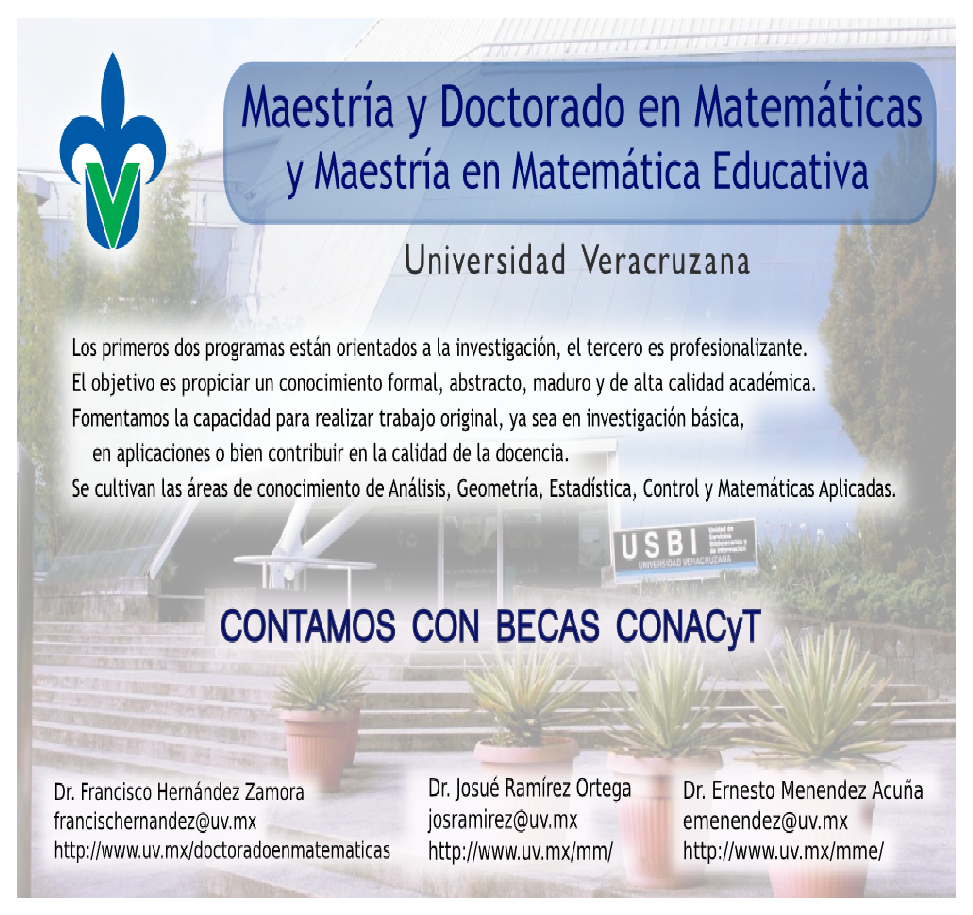
\includegraphics{otros/anuncio_VER.eps}}

\includegraphics[width=8cm,height=11cm]{anuncios/anuncio_UAEH.eps}
\hspace{1cm}
\includegraphics[width=8cm,height=11cm]{otros/POSTER-UANL.eps}
\begin{center}
\includegraphics[width=15cm,height=11cm]{anuncios/anuncio_uv.eps}
%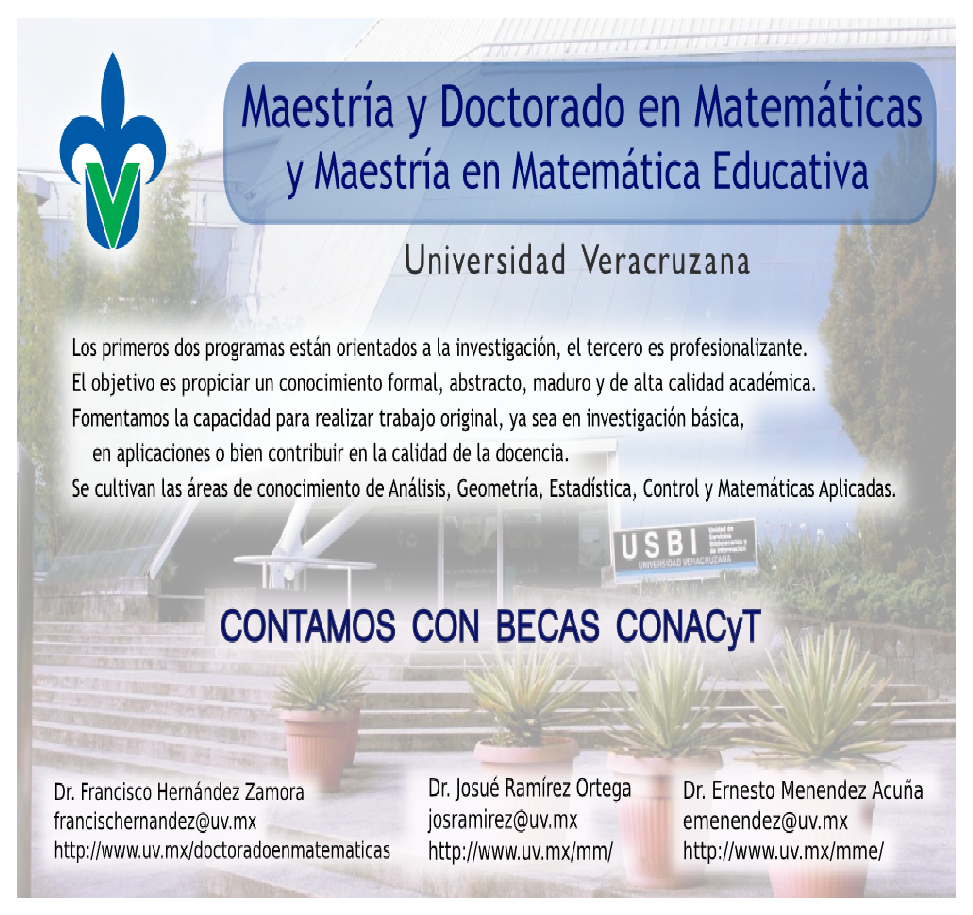
\includegraphics[width=15cm,height=11cm]{otros/anuncio_VER.eps}
\includegraphics[width=17cm]{anuncios/anuncio_memorias.eps}
\end{center}


%%%%%%%%%%%%%%%%%%%%%%%%%%%%%%%%%%%%%%%%%%%%%%%%%%%%%%%%%%%%%%%%%%
%%%%%%%%%%%%%%%%%%%%%%%%%%%%%%%%%%%%%%%%%%%%%%%%%%%%%%%%%%%%%%%%%%
%%%%%%%%%%%%                 RESUMENES                %%%%%%%%%%%%
%%%%%%%%%%%%%%%%%%%%%%%%%%%%%%%%%%%%%%%%%%%%%%%%%%%%%%%%%%%%%%%%%%
%%%%%%%%%%%%%%%%%%%%%%%%%%%%%%%%%%%%%%%%%%%%%%%%%%%%%%%%%%%%%%%%%%

\chapter{Res\'umenes}

{\sffamily	
\section*{Conferencias Plenarias}

%%%%%%%%%%%%1862%%%%%%%%%%%
\subsection*{\sffamily 1. Mis momentos favoritos de la historia de las matem�ticas (ilustrados con escenas digitales interactivas)} \label{reg-1862} \index{abreu leon jose luis@Abreu Le�n Jos� Luis!P1}
\noindent {\bfseries Jos� Luis Abreu Le�n}, {\tt joseluisabreuleon@hotmail.com}  {\slshape (Instituto de Matem�ticas de la UNAM IMATE/LITE)}\\
          \noindent La historia de las matem�ticas est� repleta de momentos emocionantes en los que se descubre algo que permite resolver un problema cient�fico importante, o aclara perfectamente alg�n tema que anteriormente era vago, o que es un m�todo sorprendentemente pr�ctico para resolver una gran variedad de problemas. En esta conferencia presentar� algunos de estos momentos que est�n entre mis favoritos, explicando en qu� consisten, porqu� fueron importantes en su momento o por su utilidad a trav�s de los siglos posteriores y analiz�ndolos en profundidad, mostrando algunos resultados que no se encuentran normalmente en los libros a pesar de pertenecer al �mbito elemental de estos temas fundamentales y a pesar de ser sumamente interesantes y elegantes. En particular trataremos: 1) La semejanza de tri�ngulos, uno de los descubrimientos matem�ticos m�s antiguos. 2) El descubrimiento de las leyes de la balanza, debido tambi�n a Arqu�medes. 3) El c�lculo de la superficie de la esfera, realizado por Arqu�medes. 4) La ca�da de los cuerpos y el tiro parab�lico, descubiertos en el Renacimiento, por Galileo principalmente. 5) El movimiento planetario, cuyas leyes fueron descubiertas por Kepler y estudiadas por Newton y otros. 6) La identidad y la igualdad de Euler, y su papel en el desarrollo del an�lisis complejo. Todos estos temas se presentar�n utilizando ilustraciones interactivas que ayudan a comprenderlos mejor y a profundizar en su significado.
%%%%%%%%%%%%1863%%%%%%%%%%%
\subsection*{\sffamily 2. Gr\'aficas extremales de cuello al menos $s$ } \label{reg-1863} \index{balbuena martinez camino@Balbuena Mart�nez Camino!P2}
\noindent {\bfseries Camino  Balbuena Mart�nez}, {\tt m.camino.balbuena@upc.edu}  {\slshape (Universidad Polit�cnica de Catalunya (UPC) /Dep. Matem�tica Aplicada III)}\\
          \noindent La clase de gr\'aficas con $n$ v\'ertices y tantas aristas como sea posible sin ciclos de la familia $\{C_3,\ldots,C_s\}$ se representa como $EX(n;\{C_3,\ldots,C_s\})$. Una gr\'afica $G\in EX(n;\{C_3,\ldots,C_s\})$  se denomina gr\'afica extremal y su n\'umero de aristas se llama n\'umero extremal. Es obvio que el cuello de una gr\'afica extremal es al menos $s$. Por esta raz\'on,  las grandes gr\'aficas construidas por los investigadores interesados en el Problema de las Jaulas proporcionan buenas cotas inferiores del n\'umero extremal. En esta charla veremos algunos valores exactos para  $s=4,5,7,10,11$ as\'\i \, como algunas cotas inferiores.
Adem\'as, revisaremos los \'ultimos resultados sobre cotas inferiores sobre el orden de $G$ y otras propiedades estructurales que garantizan que el cuello de la gr\'afica extremal es exactamente igual a $s+1$.
%%%%%%%%%%%%1864%%%%%%%%%%%
\subsection*{\sffamily 3. Retos metodol�gicos y anal�ticos de una evaluaci�n de impacto. El caso de la evaluaci�n del programa {\em 70 y m�s} } \label{reg-1864} \index{tellez rojo martha maria@T�llez Rojo Martha Mar�a!P3}
\noindent {\bfseries Martha Mar�a T�llez Rojo}, {\tt mmtellez@insp.mx}  {\slshape (Instituto Nacional de Salud P�blica)}\\
\noindent {\it  Coautores: Aar�n  Salinas-Rodr�guez, Betty  Manrique-Espinoza, Karla  Moreno}\\
\noindent Uno de los retos demogr�ficos m�s importantes a los que se enfrentar�n los pa�ses de la Am�rica Latina en el siglo XXI, ser� el incremento en el n�mero de adultos mayores (AM) y la presi�n que ejercer�n sobre los sistemas de seguridad social, asistencia m�dica y servicios para el cuidado de las personas mayores. En el caso de M�xico, la poblaci�n con la mayor tasa de crecimiento es precisamente, la poblaci�n adulta mayor. Debido a la vulnerabilidad en las condiciones de vida de los AM y como parte de las pol�ticas sociales en M�xico, en 2007 la SEDESOL implement� el Programa de Atenci�n a los Adultos Mayores de 70 a�os y m�s en zonas rurales (PAAM 70 y m�s). En sus inicios, el Programa pretendi� beneficiar a los AM de 70 a�os y m�s que habitan en localidades de no m�s de 2500 habitantes, con el prop�sito de mejorar el nivel de ingreso de los AM y, con ello, sus condiciones de vida. Actualmente, este programa se ha expandido a todo el pa�s. La puesta en marcha de un programa con este volumen de inversi�n debe acompa�arse de un proceso de evaluaci�n que permita estimar los efectos atribuibles al programa. Este objetivo implica retos metodol�gicos de diversas �ndoles. Primero, se debe proponer un dise�o de evaluaci�n de impacto que permita atribuirle al programa la causalidad de los resultados encontrados. Segundo, el an�lisis estad�stico propuesto debe responder al dise�o propuesto y a la complejidad de los diferentes dominios que se quieran evaluar. En esta pl�tica se presentar� el caso de la evaluaci�n de impacto del programa 70 y m�s en zonas rurales. Se discutir� el dise�o de evaluaci�n que propuso este grupo de investigadores que se sustenta en el modelo de regresi�n discontinua en dos dimensiones como una alternativa metodol�gica a un dise�o experimental que frecuentemente conlleva a conflictos �ticos. Asimismo, se presentar� la estrategia de an�lisis estad�stico y los principales resultados encontrados en el �rea de salud y nutrici�n.
%%%%%%%%%%%%1865%%%%%%%%%%%
\subsection*{\sffamily 4. ?`Qu� es la Matem�tica Educativa? } \label{reg-1865} \index{cantoral ricardo@Cantoral Ricardo!P4}
\noindent {\bfseries Ricardo  Cantoral}, {\tt rcantor@cinvestav.mx}  {\slshape (Centro de Investigaci�n y de Estudios Avanzados (Cinvestav). Departamento de Matem�tica Educativa (DME))}\\
          \noindent Durante la Primera Reuni�n Centroamericana y del Caribe sobre Formaci�n de Profesores e Investigaci�n en Matem�tica Educativa, en la ciudad de M�rida, mi profesor y amigo el Dr. Carlos �maz Jahnke pronunci� una conferencia plenaria con el mismo t�tulo, ?`Qu� es la Matem�tica Educativa? Siempre me intrig� el reto que �l se puso a si mismo, a 25 a�os de distancia de esa conferencia me gustar�a mostrar la evoluci�n de un dominio acad�mico que a la vez que forma parte de la Matem�tica es tambi�n componente de las Ciencias Sociales, un campo cient�fico con gran futuro y proyecci�n. Mostrar� algunos de sus resultados m�s relevantes en el marco de enfoques te�ricos robustos.\\Me ocupar� particularmente de mostrar el tr�nsito que va de la noci�n de {\it analiticidad} propia del An�lisis Matem�tico cl�sico, a la noci�n de {\it predicci�n} propia de las ciencias f�sicas con paradigma newtoniano. Analizar� la forma en que la Matem�tica Educativa construye un objeto de estudio para el desarrollo del pensamiento matem�tico de los estudiantes, estudiando los mecanismos de pasaje entre el teorema del binomio de Newton, en su forma general $(a+b)^{m\over n}$, y la teor�a de las funciones anal�ticas de Lagrange, con la serie $f(x+h)=f(x)+f^\prime(x)h+f^{\prime\prime}(x){h^2\over 2!}+\cdots$. Con estos elementos, discutiremos los resultados de un programa de profesionalizaci�n docente que se apoy� en estos resultados te�ricos.\\{\bf Referencias Bibliogr�ficas:} Cantoral, R., Tuyub, I. (2012). Construcci�n social del conocimiento matem�tico: obtenci�n de genes en una pr�ctica toxicol�gica. {\it Bolema-Boletim de Educa��o Matem�tica 26}(42A), 311-328. Bravo, S., Cantoral, R. (2012). Los libros de texto de C�lculo y el Fen�meno de la Transposici�n Did�ctica. {\it Educaci�n Matem�tica 24}(1), 5-36. Cantoral, R., L�pez-Flores, I. (2011). La Socioepistemolog�a: Un estudio de su racionalidad. {\it Paradigma 31}(1), 103-122. Brousseau, G., Caba�as, G., Cantoral, R., Oliveira, H., Da Ponte, J., Spagnolo, F. (2009). A research on classroom practice: A monograph for topic study group 24, ICME 11. {\it Quaderni di Ricerca in Didattica Scienze Matematica 4}(19), 1-6. Cantoral, R. (2010). ?`Qu� es la Matem�tica Educativa? {\it Revista Latinoamericana de Investigaci�n en Matem�tica Educativa 13}(3), 253. Cantoral, R., Farf�n, R. (2004). La sensibilit� � la contradiction: logarithmes de nombres n�gatifs et origine de la variable complexe. {\it Recherches en Didactique des Math�matiques 24}(2.3), 137-168. Cantoral, R., Ferrari, M. (2004). Uno studio socioepistemologico sulla predizione. {\it La Matematica e la sua Didattica 18}(2), 33-70. Cantoral, R., Farf�n, R. (2003). Mathematics Education: A vision of its evolution. {\it Educational Studies in Mathematics 53}(3), 255-270. Cantoral, R. (1995). Acerca de las contribuciones actuales de una did�ctica de anta�o: El caso de la Serie de Taylor. {\it Mathesis 11}(1), 55-101. Cantoral, R., Cervantes, S., Due�as, A., Pantoja, R. (1993). Generaci�n del Gr�fico de Smith usando elementos de la geometr�a moderna. {\it Revista Mexicana de F�sica 39}(2), 329-341.
%%%%%%%%%%%%1866%%%%%%%%%%%
\subsection*{\sffamily 5. On the Numerical Solution of a Nonlinear Wave Equation Associated with the $1^{\mbox{st}}$ Transcendent Painlev� Equation } \label{reg-1866} \index{glowinski roland@Glowinski Roland!P5}
\noindent {\bfseries Roland  Glowinski}, {\tt roland@math.uh.edu}  {\slshape (Department of Mathematics,  Univeristy of Houston (UH))}\\
\noindent {\it  Coautor: Annalisa Quaini}\\
\noindent  Our goal in this lecture is to address the numerical solution of the following nonlinear wave equation $${\partial^2u\over\partial^2t}-c^2\nabla^2u=6u^2+t,$$ completed by appropriate initial and boundary conditions. If $c = 0$, (NLWE) reduces to the 1st of the celebrated Painlev� transcendent equations.\\ The main difficulty with the above equation is that its solution blows-up in finite time. In order to solve (NLWE), we advocate a three-stage operator-splitting scheme whose main property is to decouple the nonlinearity and the differential operator $\nabla^2$, facilitating thus the monitoring of the solution and the adaptation of the time-discretization step when one is nearing the blow-up time. After giving a rather detailed description of the numerical methodology we employ to solve (NLWE), we will present the results of numerical experiments. These results show that our method is robust and accurate and able to capture without special difficulty the solution close to the blow-up time. The influence of c and of the boundary conditions will be also investigated.
%%%%%%%%%%%%1867%%%%%%%%%%%
\subsection*{\sffamily 6. Modelaci�n de fen�menos aleatorios en  mercados financieros } \label{reg-1867} \index{hernandez daniel@Hern�ndez Daniel!P6}
\noindent {\bfseries Daniel  Hern�ndez}, {\tt dher@cimat.mx}  {\slshape (Centro de Investigaci�n en Matem�ticas (CIMAT), Departamento de Probabilidad y Estadistica)}\\
          \noindent Los procesos estoc�sticos   permiten  describir el comportamiento de fen�menos cuyo comportamiento  no puede ser determinado con precisi�n, y poseen un gran potencial de ser aplicado en diferentes �reas, como f�sica, biolog�a o finanzas.  El an�lisis del comportamiento de los mercados financieros ha permitido establecer los fundamentos matem�ticos que, a partir de  un sistema axiom�tico,  permiten modelar las diferentes patolog�as observadas en los mercados. En esta pl�tica se presentar�n algunos de los resultados matem�ticos m�s sobresalientes que han transformado el estudio de los mercados financieros, as� como algunos de los problemas abiertos mas representativos en la actualidad.
%%%%%%%%%%%%1868%%%%%%%%%%%
\subsection*{\sffamily 7. De reacciones qu�mica oscilantes, a procesos estoc�sticos, a varias variables complejas } \label{reg-1868} \index{santillan zeron eduardo@Santillan Zeron Eduardo!P7}
\noindent {\bfseries Eduardo  Santillan Zeron}, {\tt eszeron@gmail.com}  {\slshape (IPN CINVESTAV)}\\
          \noindent Desde el primer reporte por Fechner en 1928 de una reacci�n qu�mica oscilante, �stas han sido un objeto de gran inter�s. Primero porque parecen contradecir la segunda ley de la termodin�mica y despu�s porque es dif�cil explicar la raz�n exacta de tales oscilaciones. Esta atm�sfera cambi� en 1910, cuando Lotka public�  un modelo qu�mico simple que presenta oscilaciones  amortiguadas. Hoy en d�a, el modelo simple de Lotka es ampliamente usado para analizar la propagaci�n de enfermedades infecciosas. Sin embargo, en la vida real se observan oscilaciones sostenidas en donde no deber�a de haberlas. La explicaci�n de estas discrepancias (oscilaciones sostenidas) se dedujo desde la teor�a de procesos estoc�sticos; y al fen�meno actualmente se le conoce como resonancia estoc�sticas. Aunque la idea central gira alrededor del concepto de una ``caminata aleatoria'', no es f�cil entender c\'omo estas caminatas inducen oscilaciones sostenidas en donde no deber�a de haberlas; pero m�s sorprendente a\'un es el descubrir que estas caminatas nos permiten resolver y entender problemas de ecuaciones diferenciales parciales y de varias variables complejas.
%%%%%%%%%%%%1869%%%%%%%%%%%
\subsection*{\sffamily 8. Casos de vinculaci\'on con empresas mexicanas: Problemas subyacentes } \label{reg-1869} \index{femat flores alejandro ricardo@Femat Flores Alejandro Ricardo!P8}
\noindent {\bfseries Alejandro Ricardo Femat Flores}, {\tt rfemat@ipicyt.edu.mx}  {\slshape (IPICYT)}\\
          \noindent Un incentivo para la transferencia de conocimiento es el reto de identificar los problemas cient�ficos subyacentes. Algunos problemas industriales requieren, adem�s de paciencia, de estar \'avido de encontrar e identificar problemas cient�ficos. El reto es mayor cuando el problema tecnol\'ogico absorbe el tiempo y requiere gran atenci�n para resolver lo t\'ecnico conforme al convenio. Aqu\'{\i} he elegido tres casos de vinculaci\'on con sector productivo y formulo algunos problemas matem\'aticos subyacentes. A\'un cuando se enfatiza la vinculaci\'on con empresas mexicanas, se incluye un caso ilustrativo de c\'omo se logra vinculaci\'on con empresas extranjeras. El primer caso se trata de una empresa mexicana de alimentos y sus problemas de confiter\'{\i}a. El segundo es una empresa mexicana proveedora de la industria alimenticia que produce             sabores, fragancias y colores. Por \'ultimo, una empresa francesa dedicada a la instrumentaci\'on y control para procesos biotecnol\'ogicos. Los problemas formulados tienen un car\'acter cient\'{\i`}fico y no impactan a las recetas y secrec\'{\i}a industrial sino que son nichos de oportunidad para futuros desarrollos.
%%%%%%%%%%%%1870%%%%%%%%%%%
\subsection*{\sffamily 9. Principios variacionales y formaci�n de patrones } \label{reg-1870} \index{capella kort antonio@Capella Kort Antonio!P9}
\noindent {\bfseries Antonio  Capella Kort}, {\tt capella@matem.unam.mx}  {\slshape (Instituto de Matem�ticas,  Universidad Nacional Aut�noma de M�xico (UNAM))}\\
          \noindent La formaci�n de patrones es un rasgo caracter�stico de los fen�menos que se presentan en la ciencia de materiales.  Dichos fen�menos a su vez se describen por medio de principios variacionales (o de m�nima energ�a), que generalmente son no convexos y est�n regularizados por t�rminos de orden superior. Ejemplos de este tipo de sistemas son las teor�as de Ginzburg-Landau para superconductividad los cristales l�quidos, el micromagnetismo  y las transformaciones de fase en martensitas (los llamados materiales con memoria de forma).  Nos interesa estudiar, desde un punto de vista matem�ticamente riguroso,  el l�mite singular cuando los t�rminos de orden superior  tienden a cero.  En este caso,  la incompatibilidad entre la minimizaci�n de energ�a y la no convexidad explica la formaci�n de los patrones (experimentalmente) observados y la estructura de las paredes entre los distintos dominios que componen el patr�n. En esta pl�tica daremos un panorama general de este tipo fen�menos, las t�cnicas del c�lculo de variaciones que se utilizan en su estudio y presentaremos algunos resultados relevantes para modelos particulares.


%\chapter*{Homenajes}
%\addcontentsline{toc}{section}{Homenajes}
%\chapter*{The 16th workshop on Elliptic Curve Cryptography}
%\addcontentsline{toc}{section}{The 16th workshop on Elliptic Curve Cryptography}
%\chapter*{1er Congreso Nacional de la AMITE}
%\addcontentsline{toc}{section}{1er Congreso Nacional de la AMITE}
%\chapter*{Mesas Redondas}
%\addcontentsline{toc}{section}{Mesas Redondas}
%\section{Mesas Redondas}

Los matemáticos en el sector público

Dr. Abdón Sánchez Arroyo
Banco de México
asanchez@banxico.org.mx

Dr. Jorge X. Velasco Hernández
Instituto Mexicano del Petróleo
velascoj@imp.mx

Dr. Luis M. Sanginés
Secretaría de Marina
luis_sangines@yahoo.com.mx

Moderador:
Dr. Enrique Covarrubias Jaramillo
Banco de México
ecovarrubias@banxico.org.mx

La mesa redonda está programada para el martes 30 de octubre a las 12.  Saludos a todos.

%%%%%%%%%%%%%%%%%%%%%%%%%%%%%%%%%%%%%%%%%%%


\chapter*{Sesiones Especiales}
\addcontentsline{toc}{section}{Sesiones Especiales}
{\footnotesize
\begin{center}
%\begin{tabular}{|p{50pt}|p{50pt}|p{65pt}|p{65pt}|p{65pt}|p{65pt}|p{65pt}|}
\begin{tabular}{|c|c|c|c|c|c|}
\hline[1pt]
\multicolumn{6}{|c|}{\Large\bfseries Din�mica Hamiltoniana: teor�a y aplicaciones p�g. \pageref{reg-1510}}\\
\hline
\hline
{\hfill\bfseries Hora\hfill} & {\hfill\bfseries Lunes\hfill} &  {\hfill\bfseries Martes\hfill} & {\hfill\bfseries Mi�rcoles\hfill} & {\hfill\bfseries Jueves\hfill} & {\hfill\bfseries Viernes\hfill} \\
\hline
{\hfill 9:00-9:50 \hfill} &
      &
    &
    &
        &
      \\
\cline{1-1}\cline{3-6}

{\hfill 10:00-10:20 \hfill} &
    Inauguraci�n   &
   {\bfseries \ref{reg-1510}} &
    &
    &
     \\
\cline{1-1}\cline{3-6}

{\hfill 10:20-10:40 \hfill} &
    &
   {\bfseries \ref{reg-854}} &
     &
    &
     \\
\cline{1-6}

{\hfill 10:40-11:00 \hfill} &
      &
   {\bfseries \ref{reg-1032}} &
      &
      &
     \\
\cline{1-1}\cline{3-6}

{\hfill 11:00-11:30 \hfill} &
     {\bfseries PLENARIA 1 }&
     \multicolumn{4}{|c|} {\bfseries Caf�} \\
\cline{1-6}

{\hfill 11:40-12:00 \hfill} &
     Traslado &
     {\bfseries \ref{reg-1038}} &
  &
  &
   \\
\cline{1-6}

{\hfill 12:00-12:50 \hfill} &
       &
      &
      &
   &
   \\
\cline{1-6}

{\hfill 12:50-13:00 \hfill} &
     \multicolumn{5}{|c|} {\bfseries Traslado} \\
\cline{1-6}

{\hfill 13:00-13:30 \hfill} &
       &
    {\bfseries PLENARIA  } &
    {\bfseries PLENARIA  } &
   {\bfseries PLENARIA  } &
   {\bfseries PLENARIA  } \\
%\cline{1-2}

{\hfill 13:30-13:50 \hfill} &
      &
    {\bfseries 2  } &
    {\bfseries 3  } &
   {\bfseries 4  } &
   {\bfseries 5  } \\
\cline{1-6}

{\hfill 14:00-16:30 \hfill} &
    \multicolumn{2}{|c|} {\bfseries COMIDA} &
   &
   \multicolumn{2}{|c|} {\bfseries COMIDA} \\
\cline{1-3}\cline{5-6}

{\hfill 16:40-17:00 \hfill} &
       &
   {\bfseries \ref{reg-1093}} &
     &
     &
     \\
\cline{1-1}\cline{3-3}\cline{5-6}

{\hfill 17:00-17:20 \hfill} &
      &
     {\bfseries \ref{reg-1213}} &
     &
    &
    \\
\cline{1-1}\cline{3-3}\cline{5-6}

{\hfill 17:20-17:40 \hfill} &
       &
     {\bfseries \ref{reg-1680}} &
     &
     &
     \\
\cline{1-3}\cline{5-6}

{\hfill 17:40-18:10 \hfill} &
     \multicolumn{2}{|c|} {\bfseries Caf�}&
    {\bfseries Tarde Libre} &
     \multicolumn{2}{|c|} {\bfseries Caf�} \\
\cline{1-3}\cline{5-6}

{\hfill 18:10-18:30 \hfill} &
      &
   {\bfseries \ref{reg-1192}} &
    &
   {\bfseries PLENARIA  } &
   {\bfseries PLENARIA  } \\
\cline{1-3}

{\hfill 18:30-18:50 \hfill} &
  &
    &
    &
   {\bfseries 8  } &
 {\bfseries 9  } \\
\cline{1-3}\cline{5-6}

{\hfill 18:50-19:00 \hfill} &
    \multicolumn{2}{|c|} {\bfseries Traslado} &
     &
  {\bfseries HOMENAJE} &
  {\bfseries Traslado}  \\
\cline{1-3}\cline{6-6}
{\hfill 19:00-19:50 \hfill} &
 {\bfseries  PLENARIA 6 } &
   {\bfseries  PLENARIA  7} &
       &
   {\bfseries  JORGE} &
   {\bfseries Asamblea } \\
\cline{1-3}
{\hfill 19:50-20:50  \hfill} &
  {\bfseries  HOMENAJE }&
  {\bfseries  HOMENAJE } &
       &
  {\bfseries  IZE}  &
  {\bfseries  General }  \\
  \cline{1-1}\cline{5-6}
{\hfill 20:50-21:00 \hfill} &
 {\bfseries  ERNESTO }  &
   {\bfseries FRANCISCO} &
       &
  &
   {\bfseries Traslado } \\
\cline{1-1}\cline{5-6}
    {\hfill 21:00-21:50  \hfill} &
 {\bfseries  LACOMBA } &
   {\bfseries RAGGI} &
       &
    &
   {\bfseries Clausura}   \\
\cline{1-6}

\hline[1pt]
\multicolumn{6}{|c|}{\large\bfseries Sal�n I9 }\\
\hline
\end{tabular}
\end{center}

}

\begin{multicols}{2}
\raggedcolumns

%%%%%%%%%%1510%%%%%%%%%%
\noindent \ref{reg-1510} {\bfseries Din�mica en la DNLSE  y modelos afines}\\
{\slshape Carlos Leopoldo Pando Lambruschini} {\footnotesize (RI, Inv)}\\

%%%%%%%%%%854%%%%%%%%%%
\noindent \ref{reg-854} {\bfseries Sistemas perturbados: ser lineal o bifurcar en el intento y \'erase una vez el \'indice de Conley}\\
{\slshape Nancy Leticia Gonz�lez Morales} {\footnotesize (RI, Inv)}\\

%%%%%%%%%%1032%%%%%%%%%%
\noindent \ref{reg-1032} {\bfseries Aproximaci�n por �ptica geom�trica para la transferencia y captura de exceso de electrones}\\
{\slshape Luis Alberto Cisneros Ake} {\footnotesize (RI, Inv)}\\

%%%%%%%%%%1038%%%%%%%%%%
\noindent \ref{reg-1038} {\bfseries Estabilizaci�n por resonancia param�trica del levitr\'on}\\
{\slshape Arturo Olvera Ch�vez} {\footnotesize (RI, Inv)}\\

%%%%%%%%%%1093%%%%%%%%%%
\noindent \ref{reg-1093} {\bfseries Estabilidad de los equilibrios relativos piramidales en el problema curvado de los  $4$--cuerpos con curvatura positiva}\\
{\slshape Ernesto P�rez-Chavela} {\footnotesize (RI, Inv)}\\

%%%%%%%%%%1213%%%%%%%%%%
\noindent \ref{reg-1213} {\bfseries Geometr�a en la ecuaci�n de Sine-Gordon}\\
{\slshape Gustavo Cruz-Pacheco} {\footnotesize (RI, Inv)}\\

%%%%%%%%%%1680%%%%%%%%%%
\noindent \ref{reg-1680} {\bfseries Teor�a KAM en cadenas Hamiltonianas}\\
{\slshape Jorge Viveros Rogel} {\footnotesize (RI, Inv)}\\

%%%%%%%%%%1192%%%%%%%%%%
\noindent \ref{reg-1192} {\bfseries Localizaci�n espacial en cadenas nolineales}\\
{\slshape Panayiotis Panayotaros, Francisco Mart�nez} {\footnotesize (RI, Inv)}\\

\end{multicols}

\section{XVII Encuentro de Escuelas de Matem�ticas}

\subsection{Presentaci�n} \label{encesc01}

\subsection{An�lisis, discusi�n y acuerdo sobre el car�cter de la Organizaci�n Nacional de Instituciones de Matem�ticas (ONIM); y v�nculos con otros comit�s} \label{encesc02}

\subsection{Art�culo de ONIM en reforma de estatutos de la SMM que considere acuerdos tomados y relaciones con otros comit�s} \label{encesc03}

\subsection{Elecci�n de responsables y mecanismos de trabajo y reuniones del comit� y sus coordinadores} \label{encesc04}

\subsection{Inventario de recursos humanos e infraestructura} \label{encesc05}

\subsection{Programa de capacitaci�n nacional y conferencias a distancia} \label{encesc06}

\subsection{Portal y Red Inernet, Red de Capacitadores} \label{encesc07}

\subsection{Evaluaciones y Acreditaciones; CAPEM} \label{encesc08}

\subsection{Bibliotecas m�nimas} \label{encesc09}

\subsection{Proyecto CONACYT sobre redes tem�ticas y convenios} \label{encesc10}

\subsection{Asuntos generales} \label{encesc11}



\section{Innovaci�n en Tecnolog�a Educativa}


%%%%%%%%%%%%539%%%%%%%%%%%%
\subsection{Uso de dispositivos m�viles en la ense�anza de la geometr�a: Geolab {\footnotesize (CDV, Bach)}} \label{reg-539} \index{hernandez garciadiego carlos@Hern�ndez Garciadiego Carlos!\ref{reg-539}}
\noindent{\bfseries Carlos Hern�ndez Garciadiego}, {\tt carlosh@unam.mx} {\slshape (Instituto de Matem�ticas, UNAM)}\\
\noindent En esta pl�tica se hablar� de c�mo naci� Geolab y c�mo ha ido
evolucionando para adaptarse al avance de la tecnolog�a desde las
computadoras de escritorio sin conexi�n a Internet hasta los
dispositivos m�viles como las tabletas y los tel�fonos celulares,
pasando por Enciclomedia.Se mostrar� c�mo se hacen construcciones
geom�tricas y lecciones interactivas como soporte para la ense�anza de
la geometr�a y geometr�a anal�tica para diferentes ambientes y
dispositivos

%%%%%%%%%%%%779%%%%%%%%%%%%
\subsection{Matem�TICas versus Innovaci�n {\footnotesize (CPI, Sec)}} \label{reg-779} \index{madrigal muga juan salvador@Madrigal Muga Juan Salvador!\ref{reg-779}}
\noindent{\bfseries Juan Salvador Madrigal Muga}, {\tt juan.madrigal@platea.pntic.mec.es} {\slshape (Proyecto Descartes)}\\
\noindent El Proyecto Descartes permite dar un nuevo enfoque innovador a la
ense�anza y aprendizaje de las Matem�tica en la Ense�anza Secundaria,
bajo la apariencia de un simple cambio de los medios did�cticos este
proyecto persigue un cambio m�s amplio: transformar no solo los medios
y las metodolog�as sino tambi�n los objetivos y los contenidos para
alcanzar el nivel de competencias que requiere la juventud en una
sociedad tecnol�gicamente avanzada.  La propia herramienta Descartes,
en permanente evoluci�n, los contenidos digitales interactivos
producidos con ella y la experimentaci�n llevada a cabo en las aulas
hacen vislumbrar, en un futuro pr�ximo, ese profundo cambio curricular
bajo un nuevo paradigma centrado en el aprendizaje m�s que en la
ense�anza, y ese futuro ser� tanto m�s pr�ximo cuanto antes las
administraciones educativas y entidades responsables de la formaci�n
del profesorado tomen conciencia de la obsolescencia del curr�culo
actual.


%%%%%%%%%%%%1918%%%%%%%%%%%%
\subsection{Innovaci�n en Tecnolog�a Educativa: Caso India {\footnotesize (CPI, Inv)}} \label{reg-1918} \index{pitroda sam@Pitroda Sam!\ref{reg-1918}}
\noindent{\bfseries Sam Pitroda}, {\tt elsy.sirenia@gmail.com} {\slshape (Adviser to the Prime Minister of India on Public Information Infrastructure and Innovations)} \\
\noindent Se expondr� el caso de Innovaci�n Educativa en la India desde
los �ltimos 25 a�os desde la Comisi�n Nacional del
Conocimiento. Se expondr� la agenda digital de la India para los
siguientes 25 a�os.

%%%%%%%%%%%%innmat01%%%%%%%%%%%%
\subsection{Por anunciar} \label{reg-innmat01} \index{calles martinez alipio gustavo@Calles Mart�nez Alipio Gustavo!\ref{reg-innmat01}}
\noindent{\bfseries Alipio Gustavo Calles Mart�nez}, {\tt calles@unam.mx} {\slshape (Facultad de Ciencias, UNAM)}\\


%%%%%%%%%%%%1524%%%%%%%%%%%%
\subsection{El futuro de las tecnolog�as digitales en la educaci�n matem�tica: treinta a�os despu�s de investigaci�n intensiva en el campo {\footnotesize (CPI, Sec)}} \label{reg-1524} \index{rojano ceballos maria teresa@Rojano Ceballos Mar�a Teresa!\ref{reg-1524}}
\noindent{\bfseries Mar�a Teresa Rojano Ceballos}, {\tt trojano@cinvestav.mx} {\slshape (Centro de Investigaci�n y de Estudios Avanzados (Cinvestav) del Instituto Polit�cnico Nacional (IPN) Departamento de Matem�tica Educativa)}\\
\noindent En su conferencia plenaria del 2010, en el congreso del ``17th ICMI
Study: Mathematics Education and Technology-Rethinking the Terrain'',
Seymour Papert se�al� que si bien ha sido importante investigar c�mo
el conocimiento existente puede ser aprendido (y ense�ado) en entornos
tecnol�gicos, ped�a a la audiencia de investigadores que dedic�ramos
un 10\% de nuestras reflexiones durante la reuni�n a considerar qu�
nuevos tipos de pr�cticas y conocimientos matem�ticos podr�an emerger,
como resultado del acceso a un uso efectivo de las tecnolog�as
digitales. Siguiendo el esp�ritu de la sugerencia de Seymour, en esta
ponencia har� una reflexi�n sobre c�mo la evoluci�n tecnol�gica, junto
con la experiencia acumulada de 30 a�os de investigaci�n intensiva
sobre su uso en la educaci�n matem�tica, pueden llegar a influir en el
futuro en el curr�culo oficial y en el curr�culo que en realidad se
implementa en la pr�ctica cotidiana del aula de matem�ticas (enactive
curriculum). M�s all� de la posibilidad de un acceso temprano a ideas
poderosas en matem�ticas que ofrecen los entornos tecnol�gicos de
aprendizaje, sus potencialidades did�cticas probadas (de naturaleza
cognitiva y epistemol�gica) hacen suponer que su influencia podr�a
llegar a moldear un curr�culo de matem�ticas completamente nuevo. Sin
embargo, esta posibilidad ha sido tema de acalorados debates en la
comunidad internacional de matem�ticos y especialistas en educaci�n
matem�tica. En mi presentaci�n, me referir� a dos posturas extremas a
este respecto y tratar� de plantear los pros y los contras de una y de
otra.


%%%%%%%%%%%%841%%%%%%%%%%%%
\subsection{An�lisis sem�ntico de lenguaje natural  con �rboles l�gico-sem�nticos {\footnotesize (RI, Bach)}} \label{reg-841} \index{stalmans tine@Stalmans Tine!\ref{reg-841}}
\noindent{\bfseries Tine Stalmans}, {\tt tinestalmans@gmail.com} {\slshape (Laboratorio para la Innovaci�n en Tecnolog�a Educativa (LITE))}\\
\noindent El proyecto Di�logos Inteligentes tiene como objetivo la
creaci�n de un conjunto de herramientas digitales que permiten que el
usuario (alumno) entable una conversaci�n con un tutor virtual, con el
fin de explorar y aprender alg�n tema de inter�s educativo. Como estos
di�logos se desarrollan a manera de
pregunta-respuesta-retroalimentaci�n (feedback), para que el tutor
virtual pueda dar retroalimentaciones significativas y precisas en
funci�n de las ideas y los conocimientos previos de cada persona, la
elaboraci�n de algoritmos capaces de hacer una ``lectura'' sem�ntica
adecuada de las contestaciones del alumno es una parte fundamental del
proyecto.  En esta ponencia se presentar�n los algoritmos de an�lisis
sem�ntico de lenguaje natural elaborados en el marco de este
proyecto. La metodolog�a elegida consiste en comparar lo que escribe
el usuario con una serie de respuestas esperadas -que pueden ser
correctas, incorrectas o parcialmente correctas-, cuyo significado se
codifica como ``patr�n l�gico-sem�ntico''. Estos patrones est�n
conformados por claves sem�nticas que se unen mediante operadores
l�gicos (AND, OR, NOT, NEG, MAS), formando as� un �rbol binario que
expresa un significado s. Tambi�n se presentar� un algoritmo de
correcci�n de errores ortogr�ficos comunes en espa�ol.

%%%%%%%%%%%%1133%%%%%%%%%%%%
\subsection{Descartes: Asistente y Mediador Metodol�gico {\footnotesize (CDV, Sec)}} \label{reg-1133} \index{galo sanchez jose@Galo S�nchez Jos�!\ref{reg-1133}}
\noindent{\bfseries Jos� Galo S�nchez}, {\tt jose.galo@roble.pntic.mec.es} {\slshape (Ministerio de Educaci�n, Cultura y Deporte (MECD) de Espa�a Proyecto Descartes)}\\
\noindent El proyecto Descartes del Ministerio de Educaci�n, Cultura y
Deporte de Espa�a tiene como objetivo la innovaci�n en la ense�anza y
aprendizaje de las Matem�ticas utilizando las Tecnolog�as de la
Informaci�n y de la Comunicaci�n (TIC). Para la consecuci�n de este
objetivo se dispone de una herramienta, de igual nombre, que ha
permitido el desarrollo de un amplio banco de recursos educativos
interactivos que act�an como asistentes y mediadores que catalizan el
cambio metodol�gico en el aula y contribuyen a la mejora
educativa. Las TIC han introducido un dr�stico y veloz cambio en la
Sociedad. Las pol�ticas globales y las educativas en particular buscan
permeabilizar la Sociedad de la Informaci�n y la de la Formaci�n en la
Sociedad del Conocimiento. La Escuela, s�ntesis intergeneracional,
acoge una brecha tecnol�gica generacional que pone en cuesti�n
metodolog�as y procedimientos de aprendizaje. El paso a aulas
tecnificadas no va aunado con el adecuado cambio metodol�gico, se
introducen nuevos recursos en modelos previamente establecidos y las
experiencias se centran en usos espor�dicos, no sistem�ticos, aislados
y de corta duraci�n. En el contexto educativo se constata y vuelve a
manifestarse la habitual, casi idiosincr�sica, ``Cultura del rechazo''
cuyo germen quiz�s pueda situarse en la no consecuci�n de la necesaria
``invisibilidad tecnol�gica''. En esta ponencia se muestra la diversidad
de los materiales desarrollados con Descartes y se pone de manifiesto
c�mo la utilizaci�n de estos mediadores virtuales favorece globalmente
tanto la formaci�n matem�tica concreta como la abstracta. Se incide
principal y esencialmente en las propuestas metodol�gicas que de
manera natural surgen al usarlos en el aula. Partiendo de ejemplos
donde el recurso se usa s�lo como elemento de representaci�n gr�fica
en modelos tradicionales transmisores -como mera pizarra digital-,
progresivamente se ir� detallando y profundizando en el potencial
did�ctico que la interactividad alumnado-m�quina aporta a la
construcci�n del conocimiento significativo, potenciando
simult�neamente tanto la ``autonom�a personal'', el ``aprender a
aprender'' y la formaci�n competencial. Igualmente se expone c�mo la
utilizaci�n de los recursos de Descartes adentra al profesorado en una
reflexi�n sobre su labor docente y cuestiona acerca de las rutinas
profesionales.


%%%%%%%%%%%%1910%%%%%%%%%%%%
\subsection{El Ciclo Educaci�n-Tecnolog�a {\footnotesize (CPI, Bach)}} \label{reg-1910} \index{cervantes francisco@Cervantes Francisco!\ref{reg-1910}}
\noindent{\bfseries Francisco Cervantes}, {\tt elsa\_sirenia@hotmail.com} {\slshape (Centro de Ciencias Aplicadas y Desarrollo Tecnol�gico (CCADET-UNAM))}\\
\noindent Los Sistemas y Ambientes Educativos requieren, en la
actualidad, de un uso apropiado de las Tecnolog�as Digitales, que
responda a las necesidades planteadas por las nuevas propuestas
emanadas de la Psicolog�a Educativa (Aprendizaje) y la Pedagog�a
(Ense�anza), as� como de las nuevas formas de organizaci�n, y de
gesti�n, de las Instituciones Educativas que demanda una Sociedad de
la Informaci�n, del Conocimiento y del Aprendizaje. En esta pl�tica se
presenta un proyecto donde se establece un Ciclo de interacci�n entre
las �reas de Educaci�n con las de las Tecnolog�as Digitales, para
integra tecnolog�as emergentes (Contenido Abierto, Anal�tica del
Aprendizaje, etc.), en la construcci�n de un espacio de aprendizaje
que apoye, de manera extracurricular, a los estudiantes en el
mejoramiento de su desempe�o acad�mico.

%%%%%%%%%%%%1903%%%%%%%%%%%%
\subsection{Pasado, presente y futuro de proyectos tipo Enciclomedia {\footnotesize (CPI, Pri)}} \label{reg-1903} \index{bracho carpizo felipe@Bracho Carpizo Felipe!\ref{reg-1903}}
\noindent{\bfseries Felipe Bracho Carpizo}, {\tt lillyben@hotmail.com} {\slshape (Direcci�n General de Computo y de Tecnolog�as de la Universidad Aut�noma de M�xico (UNAM))}\\
\noindent Se presentar� el proyecto Enciclomedia que se instal� en
150,000 escuelas de todo el pa�s, y se describir�n las dificultades
por las que pas� y sus principales logros. Se expondr� en especial el
proyecto Ingl�s Enciclomedia, sus logros y sus vicisitudes.
Finalmente se expondr� el nuevo esquema para ordenar recursos
did�cticos digitales alrededor del curr�culum y los beneficios que
puede aportar a los procesos de ense�anza y aprendizaje
      % 26
\section{La SMM en el Bachillerato}



%%%%%%%%%%%%1898%%%%%%%%%%%%
\subsection{La calculadora del ``Reto en 47 segundos'' {\footnotesize (CDV, Pri)}} \label{reg-1898} \index{gomez ricardo@G�mez Ricardo!\ref{reg-1898}}
\noindent{\bfseries Ricardo G\'omez}, {\tt rgomez@matem.unam.com} {\slshape (Instituto de Matem�ticas, Universidad Nacional Aut�noma de M�xico (UNAM))}\\
\noindent Veremos y analizaremos un programa que resuelve en forma
�ptima el juego de un concurso de TV que consiste en acercarse lo m�s
posible a una ``meta'' (un n�mero dado) con un conjunto de n�meros y
operaciones tambi�n dados, en no m�s de 47 segundos. Discutiremos los
aspectos combinatorios y observaremos algunas relaciones con conocidas
estructuras como los n�meros de Schr�der.

%%%%%%%%%%%%1897%%%%%%%%%%%%
\subsection{Algunas consideraciones filos�ficas sobre la demostraci�n matem�tica {\footnotesize (CDV, Pri)}} \label{reg-1897} \index{mora emiliano@Mora Emiliano!\ref{reg-1897}}
\noindent{\bfseries Emiliano Mora}, {\tt emailiano@gmail.com} {\slshape (Facultad de Filosof�a y Letras, Universidad Nacional Aut�noma de M�xico)}\\
\noindent La demostraci�n matem�tica ha sido objeto de numerosos
estudios y teor�as en filosof�a, en esta pl�tica, revisaremos
demostraciones que ponen en juego la noci�n cl�sica de la prueba,
resaltando aspectos de inter�s filos�fico y matem�tico, sobre todo en
demostraciones de gran extensi�n y que involucran uso de computadoras.

%%%%%%%%%%%%1899%%%%%%%%%%%%
%% cambio
%%\subsection{La firma del diablo {\footnotesize (CDV, Pri)}} \label{reg-1899} \index{araujo gabriela@Araujo Gabriela!\ref{reg-1899}}
%%\noindent{\bfseries Gabriela Araujo}, {\tt gabyaraujop@gmail.com} {\slshape (Instituto de Matem�ticas, Universidad Nacional Aut�noma de M�xico (UNAM))}\\
\subsection{Por anunciar {\footnotesize }} \label{smmbach01} \index{torres roberto@Torres Roberto!\ref{smmbach01}}
\noindent{\bfseries Roberto Torres} {\tt } {\slshape } \\

%%%%%%%%%%%%1893%%%%%%%%%%%%
%\subsection{Las matem�ticas en la industria {\footnotesize (CDV, Pri)}} \label{reg-1893} \index{garcia colin natalia@Garc�a Col�n Natalia!\ref{reg-1893}}
%\noindent{\bfseries Natalia Garc�a Col�n}, {\tt garciacolin.natalia@gmail.com} {\slshape (Instituto de Matem�ticas, Universidad Nacional Aut�noma de M�xico (UNAM))}\\
%\noindent En esta pl�tica presentaremos distintos rumbos de carrera
%que puede tomar un matem�tico despu�s de culminar sus estudios de
%licenciatura.

%%%%%%%%%%%%1892%%%%%%%%%%%%
%\subsection{Billares en mesas triangulares {\footnotesize (CDV, Pri)}} \label{reg-1892} \index{valdez ferran@Valdez Ferr\'an!\ref{reg-1892}}
%\noindent{\bfseries Ferr\'an Valdez}, {\tt ferran@matmor.unam.mx} {\slshape (Centro de Ciencias Matem�ticas, Universidad Nacional Aut�noma de M�xico (UNAM))}\\
%\noindent En esta pl�tica analizaremos uno de los problemas abiertos
%m�s antiguos en la teor�a de billares triangulares: la existencia de
%�rbitas peri�dicas.

%%%%%%%%%%%%1896%%%%%%%%%%%%
\subsection{Bolitas y palitos: una manera de hacer matem�ticas {\footnotesize (CDV, Pri)}} \label{reg-1896} \index{guevara aguirre mucuy-kak del carmen@Guevara Aguirre Mucuy-kak del Carmen!\ref{reg-1896}}
\noindent{\bfseries Mucuy-kak del Carmen Guevara Aguirre}, {\tt mucuy-kak.guevara@ciencias.unam.mx} {\slshape (Facultad de Ciencias, Universidad Nacional Aut�noma de M�xico (UNAM))}\\
\noindent Cuando un matem�tico dice que hace matem�ticas lo primero
que le preguntan es la ra�z cuadrada de alg�n n�mero m�s o menos
grande o una multiplicaci�n de dos n�meros con varios d�gitos (m�s de
3 casi siempre). Pero muy rara vez podr� contestar correctamente el
resultado. ?`Te imaginas a un matem�tico dibujando en un papel puntos
(bolitas) y l�neas (palitos) que los unan y que diga que est� haciendo
matem�ticas? Pues s�, \'esa es una manera de hacer matem�ticas que modela
y resuelve muchos problemas de tu vida cotidiana como por ejemplo en
las redes sociales, en el transporte p�blico o de carga, en la
asignaci�n de tus horarios y los de todos tus compa�eros de escuela, en el
uso de tu smart phone o no tan ``smart''. En esta pl�tica presentar�
la Teor�a de Gr�ficas que forma parte de un �rea de las Matem�ticas y
mostrar� los tipos de problemas que se tratan y algunos resultados que
los resuelven.


%%%%%%%%%%%%1892%%%%%%%%%%%%
\subsection{Billares en mesas triangulares {\footnotesize (CDV, Pri)}} \label{reg-1892} \index{valdez lorenzo jose ferran@Valdez Lorenzo Jos� Ferr�n!\ref{reg-1892}}
\noindent{\bfseries Jos� Ferr�n Valdez Lorenzo}, {\tt ferran@matmor.unam.mx} {\slshape (Centro de Ciencias Matem�ticas, Universidad Nacional Aut�noma de M�xico (UNAM))}\\
\noindent En esta pl�tica analizaremos uno de los problemas abiertos
m�s antiguos en la teor�a de billares triangulares: la existencia de
�rbitas peri�dicas.


%%%%%%%%%%%%1893%%%%%%%%%%%%
\subsection{Las matem�ticas en la industria {\footnotesize (CDV, Pri)}} \label{reg-1893} \index{garcia colin natalia@Garc�a Col�n Natalia!\ref{reg-1893}}
\noindent{\bfseries Natalia Garc�a Col�n}, {\tt garciacolin.natalia@gmail.com} {\slshape (Instituto de Matem�ticas, Universidad Nacional Aut�noma de M�xico (UNAM))}\\
\noindent En esta pl�tica presentaremos distintos rumbos de carrera
que puede tomar un matem�tico despu�s de culminar sus estudios de
licenciatura.


%%%%%%%%%%%%1900%%%%%%%%%%%%
\subsection{?`Por qu� los ni�os dibujan las sillas chuecas? {\footnotesize (CDV, Pri)}} \label{reg-1900} \index{morales efren@Morales Efren!\ref{reg-1900}}
\noindent{\bfseries Efr\'en Morales}, {\tt efren.morales.amaya@cimat.mx} {\slshape (Unidad Acad�mica Facultad de Matem�ticas, Universidad Aut�noma de Guerrero)}\\
\noindent Se dar� una visi�n panor�mica de los conceptos de la
geometr�a, partiendo de Euclides hasta llegar a Desargues, se har�
hincapi� en las nociones de perspectiva y simetr�a, se discutir�n
algunos elementos geom�tricos de obras maestras de la pintura.

%%%%%%%%%%%%1895%%%%%%%%%%%%
\subsection{El problema de los cuatro colores y lo que surgi� alrededor {\footnotesize (CDV, Pri)}} \label{ref-1895} \index{montejano cantoral amanda@Montejano Cantoral Amanda!\ref{ref-1895}}
\noindent{\bfseries Amanda Montejano Cantoral}, {\tt montejano.a@gmail.com} {\slshape (Facultad de Ciencias, Unidad Juriquilla, Universidad Nacional Aut�noma de M�xico (UNAM))}\\
\noindent ?`Ser� posible colorear los estados de la Rep�blica Mexicana
con tres colores de modo que estados vecinos reciban diferente color?
?`Y con cuatro colores, ser� posible? Mejor a�n ?`cu�l es el m�nimo
n�mero de colores que requerimos para colorear correctamente el mapa
de M�xico? El problema que en el p�rrafo anterior se plantea (pero
considerando cualquier mapa) es uno de los problemas m�s famosos en
matem�ticas. Se llama el problema de los cuatro colores y data de
mediados del siglo XIX. Su formulaci�n es la siguiente: ?`Pueden ser
coloreadas con cuatro, o menos colores, todas las regiones de
cualquier mapa, de modo que dos regiones con frontera com�n reciban
distinto color? La pregunta es sencilla, y la respuesta podr�a parecer
de f�cil argumento. Sin embargo, m�s de 150 a�os le cost� a la
humanidad demostrar que s�, es cierto: cualquier mapa se puede
colorear con cuatro colores o menos. Tal aseveraci�n se conoce como el
teorema de los cuatro colores, y m�s all� de su certeza lo
verdaderamente importante fue lo que naci� alrededor: la teor�a de
coloraciones en gr�ficas. ?`Qu� es lo que est� detr�s del problema de
los cuatro colores? ?`Qu� estudia en el fondo la teor�a de coloraciones
en gr�ficas? Son algunas de las preguntas que contestaremos en est�
pl�tica.

%%%%%%%%%%%%1901%%%%%%%%%%%%
%\subsection{Un poco de Mate {\footnotesize (CDV, Pri)}} \label{reg-1901} \index{juarez alejandro@Ju�rez Alejandro!\ref{reg-1901}}
%\noindent{\bfseries Alejandro Ju�rez}, {\tt garciacolin.natalia@gmail.com} {\slshape (Facultad de Ciencias, Universidad Nacional Aut�noma de M�xico (UNAM))}\\
\subsection{Un poco de Mate {\footnotesize (CDV, Pri)}} \label{reg-1901} \index{martinez leonardo@Mart�nez Leonardo!\ref{reg-1901}}
\noindent{\bfseries Leonardo Mart�nez} \\ %, {\tt garciacolin.natalia@gmail.com} {\slshape (Facultad de Ciencias, Universidad Nacional Aut�noma de M�xico (UNAM))}\\

%%%%%%%%%%%%1894%%%%%%%%%%%%
\subsection{Geometr�a a nuestro alrededor {\footnotesize (CDV, Pri)}} \label{reg-1894} \index{juan pineda daniel@Juan-Pineda Daniel!\ref{reg-1894}}
\noindent{\bfseries Daniel Juan-Pineda}, {\tt daniel@matmor.unam.mx} {\slshape (Centro de Ciencias Matem�ticas, Universidad Nacional Aut�noma de M�xico (UNAM))}\\
     % 27
\section{Las Matem�ticas en las Licenciaturas}



%%%%%%%%%%%%1874%%%%%%%%%%%%
\subsection{Tecnolog�a de Informaci�n y Estad�stica en Finanzas {\footnotesize (CDV, 1Lic)}} \label{ref-1874} \index{ortigoza alvarez giovana@Ortigoza �lvarez Giovana!\ref{ref-1874}}
\noindent{\bfseries Giovana Ortigoza �lvarez}, {\tt giovana\_harrypotter@hotmail.com} {\slshape (Universidad Aut�noma de Quer�taro)}\\
\noindent Uno de los objetivos principales de las Finanzas es
satisfacer las necesidades de cierto sector (ya sea p�blico o privado)
mediante el estudio del Capital (dinero). Dicho estudio ayuda a la
planificaci�n, ejecuci�n y control de las transacciones econ�micas o
transferencias de recursos financieros, y es aqu� donde se intercepta
con las Matem�ticas para dar paso al estudio y modelado de
las diferentes complicaciones durante su estudio encaminado a la
soluci�n de problemas nacionales e internacionales dentro de la
Econom�a. El trabajo se propone abarcar una introducci�n sobre la
necesidad y el impacto de la tecnolog�a de informaci�n y de la
estad�stica en el campo de las finanzas. Se describir� la situaci�n y
relaci�n actual entre las finanzas y la tecnolog�a de informaci�n tanto
en M�xico como en Estados Unidos; de la misma manera se describir� y
analizar� la relaci�n entre m�todos estad�sticos, la tecnolog�a
de informaci�n y las finanzas. Se describir�n ejemplos recientes y
aplicaciones concretas de empresas a nivel mundial que han utilizado
con �xito los sistemas tecnol�gicos financieros y los m�todos
estad�sticos para desempe�ar sus funciones diarias y para
lograr ventajas competitivas mediante el uso de estos sistemas y
m�todos. Los aspectos del �rea de finanzas en las cual se enfoca este
trabajo son: presupuestos y planeaci�n, an�lisis financiero, cierres
financieros de mes, tesorer�a, administraci�n de inventario, cr�ditos y
cobranzas y cuentas por pagar. Al final de este trabajo se presenta una
conclusi�n de los beneficios y del valor agregado de utilizar la
tecnolog�a de informaci�n en el �rea de finanzas. Por la parte de
estad�stica usaremos proyecciones y predicciones.

%%%%%%%%%%%%1875%%%%%%%%%%%%
\subsection{Percolaci�n Topol�gica y Homolog�a Persistente {\footnotesize (CDV, 2Lic)}} \label{reg-1875} \index{pitones amaro yuriko@Pitones Amaro Yuriko!\ref{reg-1875}}
\noindent{\bfseries Yuriko Pitones Amaro}, {\tt ypalob@hotmail.com} {\slshape (Universidad Aut�noma de Zacatecas)}\\
\noindent En el presente trabajo se formula el problema de
percolaci\'on sobre una superficie en t\'erminos de coberturas de
redes de sensores. Se expone un criterio homol\'ogico de cobertura
desarrollado en el art\'iculo {\slshape Homological Sensor Networks} de Vin
de Silva and Robert Ghrist. Se iniciar\'a introduciendo conceptos
b\'asicos de Topolog\'ia Algebr\'aica, para continuar con los
preliminares de la Teor\'ia de Homolog\'ia Simplicial y con todo esto
cumplir el objetivo planteado, para finalizar haremos una breve
introducci\'on a la Teor\'ia de Homolog\'ia Persistente.


%%%%%%%%%%%%1877%%%%%%%%%%%%
\subsection{El Polinomio de Tutte {\footnotesize (CDV, 2Lic)}} \label{reg-1877} \index{martinez rios rosal de jesus@Mart�nez R�os Rosal de Jes�s!\ref{reg-1877}}
\noindent{\bfseries Rosal de Jes�s Mart�nez R�os}, {\tt lasor\_22@yahoo.com} {\slshape (Universidad Aut�noma Benito Ju�rez de Oaxaca)}\\
\noindent El Polinomio de Tutte, un invariante de gr�ficas que es un
polinomio en dos variables, debe su importancia a las m�ltiples
interpretaciones combinatorias de diversas evaluaciones en puntos o a
lo largo de curvas algebraicas. En este trabajo presentamos una nueva
interpretaci�n de la evaluaci�n del Polinomio de Tutte en el punto
(1,-1) para las gr�ficas completas, que adem�s permite probar cierta
igualdad.

%%%%%%%%%%%%1876%%%%%%%%%%%%
\subsection{El Problema de Desviaci�n M�xima en un sistema de ecuaciones diferenciales de orden cuatro {\footnotesize (CDV, 2Lic)}} \label{reg-1876} \index{pena garcia jose alberto@Pe�a Garc�a Jos� Alberto!\ref{reg-1876}}
\noindent{\bfseries Jos� Alberto Pe�a Garc�a}, {\tt ruvelsa@yahoo.com} {\slshape (Universidad Aut�noma del Estado de Hidalgo)}\\
\noindent Mediante la aplicaci�n del Principio del M�ximo de
Pontryagin se resuelve de forma anal�tica la s�ntesis de ciclos
l�mite orbitalmente estables que satisfacen el problema de desviaci�n
m�xima en el sentido de Aleksandrov-Zhermolenko en una de las cuatro
clases del sistema de ecuaciones diferenciales de orden cuatro

\begin{equation*}
\left\{\begin{aligned} &
\ddot{\boldsymbol{x}}+A\dot{\boldsymbol{x}}+B\boldsymbol{x}=\boldsymbol{b}u_1\\ &
u_1(\cdot)\in U=\{u\in KC:|u(t)|\leq 1\}\end{aligned}\right. \qquad
\boldsymbol{x}(t)\in\mathbf{R}^2
\end{equation*}
\noindent
donde $A=(a_{ij})$ y $B=(b_{ij})$ son matrices reales constantes de
tama�o $2\times 2$, $\boldsymbol{b}$ es un vector constante de tama�o
$2\times 1$, y $u_1(\cdot)$ es una funci�n escalar (control adicional)
continua a trozos. Los resultados obtenidos se comparan con t�cnicas
num�ricas.

%%%%%%%%%%%%1393%%%%%%%%%%%%
\subsection{El comp�s de Arqu�medes y una propiedad caracter�stica de la  Elipse {\footnotesize (CDV, 1Lic)}} \label{reg-1393} \index{rosales rivera antonio@Rosales Rivera Antonio!\ref{reg-1393}}
\noindent{\bfseries Antonio Rosales Rivera}, {\tt xx\_billyxx@hotmail.com} {\slshape (Universidad Aut�noma de Quer\'etaro (UAQ))}\\
\noindent Uno de los m�todos para construir elipses es mediante el
Comp�s de Arqu�medes. A pesar de ser un m�todo que cuenta con gran
belleza y que encierra una gran cantidad de propiedades geom�tricas
interesantes, no es m�todo tan conocido como por ejemplo la
Construcci�n del Jardinero. Al analizar un poco m�s profundamente este
m�todo hemos descubierto una propiedad que caracteriza a las elipses
de entre las figuras convexas en el plano. Tal caracterizaci�n se
fundamenta en algunas t�cnicas de �lgebra vectorial y transformaciones
afines. Adem�s, es interesante c\'omo en los argumentos de la
demostraci�n se utilizan tanto el comp�s de Arqu�medes como el m�todo
de los c�rculos conc�ntricos. Adem�s, de toda la fundamentaci�n
te�rica sobre esta construcci�n, se mostrar� un mecanismo mediante el
cual se pueden dibujar elipses. De esta manera, se ver� una clara
relaci�n entre la geometr�a y la mec�nica.


%%%%%%%%%%%%598%%%%%%%%%%%%
\subsection{Grupos Kleinianos y Superficies Hiperb�licas {\footnotesize (RT, 2Lic)}} \label{reg-598} \index{tapia lorenzo maria del carmen@Tapia Lorenzo Mar�a del Carmen!\ref{reg-598}}
\noindent{\bfseries Mar�a del Carmen Tapia Lorenzo}, {\tt marlo\_tap13@hotmail.com} {\slshape (Universidad Aut�noma del Estado de Morelos (UAEM))}\\
\noindent En este trabajo estudiamos variedades hiperb�licas completas
que no son necesariamente compactas. La herramienta principal para
este estudio en el lema de Margulis, el cual puede ser enunciado de
manera heur�stica de la siguiente forma: Para cada n�mero natural n
existe una constante $\epsilon_{n}$ tal que si $M$ es una n-variedad
hiperb�lica completa y orientable, y si $x$ es un elemento de $M$ para
el cual existe un elemento del grupo fundamental de $M$ con base en
$x$ y de longitud hiperb�lica peque�a, entonces el subgrupo del grupo
fundamental generada por lazos de longitud peque�a basados en $x$, no
es muy complicado. Usando el resultado anterior, tambi�n se describen
las propiedades de descomposici�n de una variedad hiperb�lica en las
partes llamadas delgadas y gruesas. Tambi�n para el caso de variedades
de volumen finito, se da una descripci�n de la forma de terminaciones
de tales variedades.

%%%%%%%%%%%%676%%%%%%%%%%%%
\subsection{Una prueba topol�gica de la infinitud de los n�meros primos {\footnotesize (CDV, 2Lic)}} \label{reg-676} \index{munoz zepeda jesus antonio@Mu�oz Zepeda Jes�s Antonio!\ref{reg-676}}
\noindent{\bfseries Jes�s Antonio Mu�oz Zepeda}, {\tt jesss23@hotmail.com} {\slshape (Universidad Aut�noma de Chiapas (UNACH) Centro de Estudios en F�sica y Matem�ticas B�sicas y Aplicadas (CEFyMAP))}\\
\noindent En esta charla, con aspectos tan b�sicos de topolog�a como
espacios topol�gicos y conjuntos abiertos y cerrados, mostraremos una
prueba, topol�gica, de que existe una cantidad infinita de n�meros
primos.

%%%%%%%%%%%%787%%%%%%%%%%%%
\subsection{Teor�as de Homolog�a {\footnotesize (RT, 2Lic)}} \label{reg-787} \index{catalan ramirez juan jose@Catal�n Ram�rez Juan Jos�!\ref{reg-787}}
\noindent{\bfseries Juan Jos� Catal�n Ram�rez}, {\tt rincon\_de\_pitagoras@hotmail.com} {\slshape (Universidad Aut�noma del Estado de Morelos (UAEM))}\\
\noindent Una teor\'ia de homolog\'ia reducida definida en una familia de
parejas de espacios topol\'ogicos $F$ consiste en los
siguiente:

\begin{itemize}
\item Una familia \{$\widetilde{H}_{q}
  \,|\, q \in$ $\mathbb{Z}$ \} tal que cada $\widetilde{H}_{q}$ asigna
  a cada pareja $(\cal{X},A)$ $\in$ F un grupo abeliano
  $\widetilde{H}_{q}(\cal{X},A)$.
  \vskip .1cm
Este grupo se llama el $q$-\'esimo
  grupo de homolog\'ia relativa de $\cal{X}$ mod A.
  \vskip .2cm
\item
  Para cada funci\'on continua $f:(\cal{X},A)\rightarrow(\cal{Y},B)$
  donde $(\cal{X},A)$, $(\cal{Y},B)$ $\in$ $F$, existe un homomorfismo
  inducido
  $f_{\ast,q}:\widetilde{H}_{q}(\cal{X},A)\rightarrow$$\widetilde{H}_{q}(\cal{Y},B)$
  para todo $q$.
  \vskip .2cm
\item Para cualquier $(\cal{Y},B)$ $\in$
  $F$ y para cualquier entero $q$ existe un homorfismo
  $\partial_{q}:\widetilde{H}_{q}(\cal{X},A)\rightarrow$$\widetilde{H}_{q-1}(A)$.
\end{itemize}
\vskip .5cm
Los objetos anteriores est\'an sujetos a un conjunto de axiomas, los
axiomas de S. Eilenberg y N. Steenrod.  \vskip
.3cm

\begin{enumerate}
\item Identidad. Sea
  $1_{\cal{X}}:(\cal{X},A)\rightarrow (\cal{X},A)$ la identidad.
  Entonces
  $(1_{\cal{X}})_{\ast,q}:\widetilde{H}_{q}(\cal{X},A)\rightarrow$$\widetilde{H}_{q}(\cal{X},A)$
  es la identidad.
  \vskip .3cm
\item Composici\'on. Sean
  $f:(\cal{X},A)\rightarrow (\cal{Y},B)$, $g:(\cal{Y},B)\rightarrow
  (\cal{Z},C)$ funciones continuas.
  \vskip .1cm
  Entonces $(g \circ
  f)_{\ast,q}$ = $g_{\ast,q} \circ
  f_{\ast,q}:\widetilde{H}_{q}(\cal{X},A)\rightarrow$$\widetilde{H}_{q}(\cal{Z},C)$.
\item
  Homotop�a. Sea $f,g:(\cal{X},A)\rightarrow(\cal{Y},B)$
  homot\'opicas. Entonces $f_{\ast,q}$ =
  $g_{\ast,q}:\widetilde{H}_{q}(\cal{X},A)\rightarrow$$\widetilde{H}_{q}(\cal{Y},B)$.
  \vskip .3cm
\item Exactitud. Sea $(\cal{X},A)$ una pareja de espacios
  topol\'ogicos. Entonces la siguiente sucesi\'on es exacta.
 \vskip .1cm
 $\ldots\stackrel{\partial_{q+1}}{\longrightarrow}$$\widetilde{H}_{q}(A)$$\stackrel{i_{\ast,q}}{\longrightarrow}$$\widetilde{H}_{q}(\cal{X})$$\stackrel{j_{\ast,q}}{\longrightarrow}$$\widetilde{H}_{q}(\cal{X},A)$$\stackrel{\partial_{q}}{\longrightarrow}$$\widetilde{H}_{q-1}(A)$$\stackrel{i_{\ast,q-1}}{\longrightarrow} \ldots $
\vskip .1cm
Donde $\partial_{q}$ es el homomorfismo definido
anteriormente, $i_{\ast,q}$ y $j_{\ast,q}$ son homomorfismos inducidos
por la inclusi\'on.
\item Excisi\'on. Sea $(\cal{X},A)$ una pareja de
  espacios topol\'ogicos, $U$ $\subset$ $A$ $\subset$ $\cal{X}$ tal que
  la cerradura de $U$ est\'a contenida en el interior de $A$. Entonces
  la inclusi\'on $i:(\cal{X}-U,A-U)\rightarrow (\cal{X},A)$ induce
  isomorfismos
  $i_{\ast,q}:\widetilde{H}_{q}(\cal{X}-U,A-U)\rightarrow $$\widetilde{H}_{q}(\cal{X},A)$
  para todo $q$.
  \vskip .3cm
\item Naturalidad del homorfismo
  $\partial_{q}$. Sea $f:(\cal{X},A)\rightarrow(\cal{Y},B)$ una
  funci\'on continua, $f\,|\,_{A}$ la restricci\'on de $f$ a
  $A$. Entonces $\partial_{q} \circ f_{\ast,q}$ =
  $(f\,|\,_{A})_{\ast,q-1} \circ \partial_{q}$ tal que el siguiente
  diagrama es conmutativo:
  \vskip .2cm
  $\widetilde{H}_{q}(\cal{X},A)$
  \hskip .3cm
  $\stackrel{f_{\ast,q}}{\longrightarrow}$
  \hskip .3cm
  $\widetilde{H}_{q}(\cal{Y},B)$
  \vskip .1cm
  \hskip .5cm $\downarrow_{\partial_{q}}$
  \hskip .9cm \hskip .9cm $ \downarrow_{\partial_{q}}$
  \vskip .1cm $\widetilde{H}_{q-1}(A)$
  $\stackrel{(f\,|\,_{A})_{\ast,q-1}}{\longrightarrow}$
  $\widetilde{H}_{q-1}(B)$
\item Dimensi\'on. Sea $P$ un espacio
  topol\'ogico que consiste de un %s\'olo 
punto.
  \vskip .1cm Entonces
  $\widetilde{H}_{q}(P)$ = $0$ para todo $q$ $\neq$ $0$.
\end{enumerate}

Si se omite el axioma de dimensi\'on los axiomas restantes definen lo
que se conoce como una teor\'ia de homolog\'ia generalizada. En esta
pl\'atica se describir\'a y dar\'an ejemplos de estas teor\'ias y se
explicar\'a su utilidad.

%%%%%%%%%%%%838%%%%%%%%%%%%
\subsection{Algunas propiedades del espacio euclidiano $\mathbb{R}^{n}$ que no se preservan a espacios m�tricos arbitrarios {\footnotesize (CDV, 2Lic)}} \label{reg-838} \index{gonzalez martinez nayeli adriana@Gonz�lez Mart�nez Nayeli Adriana!\ref{reg-838}}
\noindent{\bfseries Nayeli Adriana Gonz�lez Mart�nez}, {\tt eyan\_17@hotmail.com} {\slshape (Universidad Tecnol�gica de la Mixteca (UTM))}\\
\noindent El conjunto $\mathbb{R}^{n}$, de todas las $n$-adas de
n�meros reales, junto con la forma usual de medir la distancia entre
dos de ellas, es lo que se conoce como espacio m�trico euclidiano. En
esta pl�tica expondremos algunas propiedades que tiene este espacio
m�trico particular y que no se preservan a espacios m�tricos
arbitrarios.


%%%%%%%%%%%%848%%%%%%%%%%%%
\subsection{Construcci�n de una curva de Peano utilizando el conjunto de Cantor {\footnotesize (CDV, 2Lic)}} \label{reg-848} \index{morales jimenez israel@Morales Jim�nez Israel!\ref{reg-848}}
\noindent{\bfseries Israel Morales Jim�nez}, {\tt fast.ismoji@gmail.com} {\slshape (Universidad Tecnol�gica de la Mixteca (UTM))}\\
\noindent En esta pl�tica se muestra c�mo utilizar el conjunto de
Cantor y un producto infinito de espacios topol�gicos para construir
una curva que llena todo el cubo $k$-dimensional unitario
$[0,1]^{k}$.

%%%%%%%%%%%%1873%%%%%%%%%%%%
\subsection{Pol�gonos, poliedros y politopos {\footnotesize (CDV, 2Lic)}} \label{reg-1873} \index{sanchez flores lizbeth@S�nchez Flores Lizbeth!\ref{reg-1873}}
\noindent{\bfseries Lizbeth S�nchez Flores}, {\tt rcruzcast@gmail.com} {\slshape (Universidad Aut�noma del Estado de Hidalgo (UAEH))}\\
\noindent Se dar� una breve introducci�n a los pol�gonos, poliedros y
politopos.

%%%%%%%%%%%%849%%%%%%%%%%%%
\subsection{Algoritmo gen�tico para entrenamiento de redes neuronales {\footnotesize (CDV, 1Lic)}} \label{reg-849} \index{ocampo sanchez jimena@Ocampo S�nchez Jimena!\ref{reg-849}}
\noindent{\bfseries Jimena Ocampo S�nchez}, {\tt jimenaocampos.com@gmail.com} {\slshape (Universidad Aut�noma de Quer�taro (UAQ))}\\
\noindent En un problema de optimizaci�n, aparte de las condiciones
que deben cumplir las soluciones factibles del problema, se busca la
que es �ptima seg�n alg�n criterio de comparaci�n entre ellas. En
Optimizaci�n Matem�tica, el t�rmino heur�stico se aplica a un
procedimiento de resoluci�n de problemas de optimizaci�n con una
concepci�n diferente: se califica de heur�stico a un procedimiento
para el que se tiene un alto grado de confianza en que encuentra
soluciones de alta calidad con un coste computacional razonable,
aunque no se garantice su optimalidad o su factibilidad, e incluso, en
algunos casos, no se llegue a establecer lo cerca que se est� de dicha
situaci�n. Es usual aplicar el t�rmino heur�stica cuando, utilizando el
conocimiento que se tiene del problema, se realizan modificaciones en
el procedimiento de soluci�n del problema que, aunque no afectan a la
complejidad del mismo, mejoran el rendimiento en su comportamiento
pr�ctico. Los m�todos heur�sticos espec�ficos deben ser dise�ados a
prop�sito para cada problema, sin embargo, las heur�sticas generales
emanadas de las metaheur�sticas pueden mejorar su rendimiento
utilizando recursos computacionales y estrategias inteligentes. De
esta manera es como surge la aplicaci�n de inteligencia artificial en
la rama de la optimizaci�n. En este trabajo se estudia a dos de las
principales metaheur�sticas utilizadas en la optimizaci�n; los
algoritmos gen�ticos y las redes neuronales, pero no tomando cada caso
por separado si no mas bien se estudia un m�todo alternativo para el
entrenamiento de redes neuronales con conexi�n hacia adelante. Una vez
determinada la topolog�a de la red neuronal se utiliza un algoritmo
gen�tico para ajustar los pesos de la red neuronal. Se eval�an
diferentes variantes de los operadores gen�ticos para el entrenamiento
de las redes neuronales.

%%%%%%%%%%%%850%%%%%%%%%%%%
\subsection{M�trica de Hausdorff {\footnotesize (CDV, 2Lic)}} \label{reg-850} \index{hernandez hernandez pablo jorge@Hern�ndez Hern�ndez Pablo Jorge!\ref{reg-850}}
\noindent{\bfseries Pablo Jorge Hern�ndez Hern�ndez}, {\tt pablin9104\_@hotmail.com} {\slshape (Universidad Tecnol�gica de la Mixteca (UTM))}\\
\noindent Considerando un espacio m�trico $(X,d)$, en esta pl�tica
demostramos que la m�trica $d$, induce una m�trica al conjunto que
consiste de todos los subconjuntos cerrados y no vac�os de $X$,
conocida como m�trica de Hausdorff. Adem�s, exponemos algunas de sus
propiedades.


%%%%%%%%%%%%1260%%%%%%%%%%%%
\subsection{Reconstrucci�n combinatoria de curvas: el Crust de una nube de puntos {\footnotesize (CI, 1Lic)}} \label{reg-1260} \index{martinez munoz daniel antonio@Mart�nez Mu\~noz Daniel Antonio!\ref{reg-1260}}
\noindent{\bfseries Daniel Antonio Mart�nez Mu�oz}, {\tt dannyelote@gmail.com} {\slshape (Universidad Aut�noma de Ciudad Ju�rez (UACJ))}\\
\noindent Existen varias situaciones en las cuales un conjunto de
puntos situados cerca o sobre una superficie es usado para reconstruir
una aproximaci�n poligonal a la superficie. En el plano este problema
se convierte en una especie del cl�sico juego ``conecta los puntos''. La
reconstrucci�n de curvas en el plano es importante desde una visi�n
computacional. Los identificadores simples de aristas seleccionan
aquellos pixeles de la imagen que parecen pertenecer a las aristas,
generalmente delimitando las fronteras de los objetos; agrupar esos
pixeles y formar curvas hoy es un �rea de investigaci�n muy
atractiva. En este trabajo se pretende, a partir de un conjunto de
puntos en el plano que cumple ciertas condiciones de muestreo, generar
grafos basados en la proximidad de los puntos, de forma que se
garantice la reconstrucci�n de una curva suave. El grafo que aqu� se
expone es el llamado ``crust'', concepto introducido por Nina Amenta,
Marshal Bern y David Eppstein.

%%%%%%%%%%%%1927%%%%%%%%%%%%
\subsection{Equilibrios con variaciones conjeturadas en un duopolio mixto de estructura especial {\footnotesize (CDV, 2Lic)}} \label{reg-1927} \index{camacho esparza edgar@Camacho Esparza Edgar!\ref{reg-1927}}
\noindent{\bfseries Edgar Camacho Esparza}, {\tt monique\_2789@hotmail.com} {\slshape (Universidad Aut�noma de Nuevo Le�n (UANL))}\\
\noindent Consideramos un duopolio mixto en un mercado de un producto
homog�neo con la estructura del agente p�blico. Tomando en cuenta que
un duopolio mixto cuenta con dos agentes, entre los cuales hay una
compa��a (agente) p�blica la cual, en contraste al agente privado,
maximiza no la funci�n de su ganancia neta pero si el bienestar
dom�stico social. Son empleados algunos Teoremas de existencia de
equilibrios exteriores e interiores con variaciones conjeturadas (CVE)
derivados en los trabajos previos de Nataliya I. Kalashnykova y sus
coautores.

En nuestro modelo, el productor p�blico combina en forma convexa las
funciones de bienestar dom�stico social y de la ganancia neta. Bajo
suposiciones generales, se demuestra la existencia y unicidad del
equilibrio exterior (definido por las conjeturas fijas de los agentes
dadas en forma ex�gena), as� como la existencia de por lo menos un
equilibrio interior (o bien, consistente), en los cuales las
conjeturas (coeficientes de influencia) de los agentes se encuentran
en proceso de b�squeda del equilibrio mismo. Finalmente, se analiza el
comportamiento de ciertos par�metros del equilibrio interior
(consistente) en dependencia con el coeficiente de combinaci�n convexa
de las funciones objetivos en la meta del agente p�blico.
      % 28
\section{Matem�ticas en la Industria}


%%%%%%%%%%%%1909%%%%%%%%%%%%
\subsection{Aplicaciones de geometr�a diferencial en control de sistemas no lineales {\footnotesize (CDV, 1Lic)}} \label{reg-1909} \index{pineda castillo jose cruz@Pineda Castillo Jos� Cruz!\ref{reg-1909}}
\noindent{\bfseries Jos� Cruz Pineda Castillo}, {\tt jpineda@ciateq.mx} {\slshape (Centro de Tecnolog�a Avanzada (CIATEQ))}\\


%%%%%%%%%%%%1908%%%%%%%%%%%%
\subsection{Las matem�ticas de la acotaci�n funcional en el dise�o y manufactura industrial {\footnotesize (CDV, 1Lic)}} \label{reg-1908} \index{rauda rodriguez jose@Rauda Rodr�guez Jos�!\ref{reg-1908}}
\noindent{\bfseries Jos� Rauda Rodr�guez}, {\tt jose.rauda@ciateq.mx} {\slshape (Centro de Tecnolog�a Avanzada (CIATEQ))}\\
\noindent La compatibilidad entre el dise�o y la manufactura de
componentes de equipo y maquinaria requiere del dise�ador el
conocimiento de los procesos de manufactura y del ensamble piezas. La
especialidad entre ellas se denomina acotaci�n funcional que a simple
vista parece sencilla, sin embargo es la causante de p�rdidas de
productividad y eficiencia de los procesos. Las matem�ticas
involucradas en la acotaci�n funcional igualmente se aprecian
sencillas pero requieren de un razonamiento f�sico y matem�tico as�
como de la conceptualizaci�n funcional del producto. La acotaci�n
funcional toma en cuenta la habilidad de los equipos de producci�n, la
capacidad de los procesos de manufactura, la funcionalidad del
producto final en sitio, todo ello dependiente de un razonamiento
matem�tico en cada etapa para determinar dichos procesos de
fabricaci�n ensamble y operaci�n. Se muestran las consideraciones y
criterios matem�ticos y el efecto de los mismos cuando son tanto bien
como mal aplicados. Se presentan asimismo las bases de la acotaci�n
funcional y su aplicaci�n en la industria.


%%%%%%%%%%%%matind01%%%%%%%%%%%%
\subsection{La importancia de las matem�ticas en la ingenier�a {\footnotesize (CPI, 1Lic)}} \label{reg-matind01} \index{herrera ruiz gilberto@Herrera Ruiz Gilberto!\ref{reg-matind01}}
\noindent{\bfseries Gilberto Herrera Ruiz}, {\tt } {\slshape (Universidad Aut�noma de Quer�taro)}\\


%%%%%%%%%%%%1907%%%%%%%%%%%%
\subsection{Simulaci�n de ondas de choque t�ndem aplicadas a la litotricia extracorp�rea {\footnotesize (CDV, 1Lic)}} \label{reg-1907} \index{canseco lopez guillermo@Canseco L�pez Guillermo!\ref{reg-1907}}
\noindent{\bfseries Guillermo Canseco L�pez}, {\tt gcanseco@condumex.com.mx} {\slshape (Centro de Investigaci�n y Desarrollo (CIDEC))}\\
\noindent La litotricia extracorp�rea por ondas de choque es una
terapia confiable para el tratamiento de la urolitiasis. Para
optimizar este tipo de intervenci�n, es necesario hacer m�s eficiente
la fragmentaci�n que se produce de los c�lculos renales y reducir el
da�o que se ocasiona a los tejidos circundantes. Con el objetivo de
contribuir al mejoramiento de la litotricia extracorp�rea, se
analizaron los mecanismos de ruptura de los c�lculos renales y
posteriormente se propuso una modificaci�n en el mecanismo de
litotricia producido por la cavitaci�n ac�stica generada por medio de
ondas de choque. Para el logro del objetivo antes planteado, se gener�
un modelo matem�tico para simular, por medio de la formulaci�n de
Gilmore, los fen�menos f�sicos que se producen durante la cavitaci�n
de una burbuja sometida a ondas de choque t�ndem modificadas. Como el
an�lisis de los resultados de la simulaci�n se ha llegado a la
conclusi�n de que la litotricia extracorp�rea se puede mejorar con el
dise�o de un mejor perfil de presi�n de la segunda onda de choque.


%%%%%%%%%%%%1906%%%%%%%%%%%%
\subsection{Fragibility and Robustness Finite and Fixed Time Convergence in Modern Control Theory {\footnotesize (CDV, 1Lic)}} \label{reg-1906} \index{fridman leonid@Fridman Leonid!\ref{reg-1906}}
\noindent{\bfseries Leonid Fridman}, {\tt lfridman@servidor.unam.mx} {\slshape (Facultad de Ingenier�a, Universidad Nacional Aut�noma de M�xico)}\\


%%%%%%%%%%%%1905%%%%%%%%%%%%
\subsection{Bombardier Aerospace - Mathematics to fly people {\footnotesize (CDV, 1Lic)}} \label{reg-1905} \index{tessier patrick@Tessier Patrick!\ref{reg-1905}}
\noindent{\bfseries Patrick Tessier}, {\tt patrick.tessier@aero.bombardier.com} {\slshape (Bombardier Aerospace Mexico)}\\
\noindent Presentation of Bombardier Aerospace and its activities in
Mexico. Overview of the mathematics used today in the development of
new aircraft, current limitations and future needs.


%%%%%%%%%%%%1904%%%%%%%%%%%%
\subsection{Matem�ticas y trayectoria profesional {\footnotesize (CDV, 1Lic)}} \label{reg-1904} \index{gobenceaux claude@Gobenceaux Claude!\ref{reg-1904}}
\noindent{\bfseries Claude Gobenceaux}, {\tt claude.gobenceaux@safranmbd.com} {\slshape (Grupo SAFRAN Americas Division)}\\


%%%%%%%%%%%%matind02%%%%%%%%%%%%
\subsection{21st Century Competencies for Engineers {\footnotesize (CPI, 1Lic)}} \label{reg-matind02} \index{gutierrez de velasco rodriguez jorge enrique leonardo@Guti�rrez de Velasco Rodr�guez Jorge Enrique Leonardo!\ref{reg-matind02}}
\noindent{\bfseries Jorge Enrique Leonardo Guti�rrez de Velasco Rodr�guez}, {\tt jorge.gutierrezdevelazco@unaq.edu.mx} {\slshape (Universidad Aureona�tica en Quer�taro)}\\
      % 29
\section{Miscel�nea Matem�tica}


%%%%%%%%%%%%1221%%%%%%%%%%%%
\subsection{El Producto Cruz y Cantidades Conservadas {\footnotesize (1Lic, CDV)}} \label{reg-1221} \index{berlanga zubiaga ricardo@Berlanga Zubiaga Ricardo!\ref{reg-1221}}
\noindent{\bfseries Ricardo  Berlanga Zubiaga}, {\tt berlanga@servidor.unam.mx} {\slshape (Universidad Nacional Aut�noma de M�xico (UNAM)  Instituto de Investigaciones en Matem�ticas Aplicadas y en Sistemas (IIMAS)  Departamento de F�sica Matem�tica)}\\
\noindent La peculiar naturaleza del producto cruz de nuestro libro de
Geometr�a Anal�tica es un buen comienzo para hablar de la esfera en el
espacio de dimensi�n cuatro, de Grupos en tanto simetr�as y de la
Geometr�a de las leyes de conservaci�n en Mec�nica en el esp�ritu de
Emmy Noether.


%%%%%%%%%%%%700%%%%%%%%%%%%
\subsection{Soluci�n al Problema de Toma de Decisi�n Personal {\footnotesize (1Lic, CDV)}} \label{reg-700} \index{galeana sanchez hortensia@Galeana S�nchez Hortensia!\ref{reg-700}}
\noindent{\bfseries Hortensia  Galeana S�nchez}, {\tt hgaleana@matem.unam.mx} {\slshape (Instituto de  Matem�ticas UNAM)}\\
\noindent En �sta pl�tica, se plantear� y resolver� el problema de
toma de decisiones personales mediante un modelo en digr�ficas. No se
requieren conocimientos previos y se obtiene una soluci�n algor�tmica
del problema.


%%%%%%%%%%%%1407%%%%%%%%%%%%
\subsection{Poliedros proyectos {\footnotesize (1Lic, CDV)}} \label{reg-1407} \index{hubard isabel@Hubard Isabel!\ref{reg-1407}}
\noindent{\bfseries Isabel  Hubard}, {\tt hubard@matem.unam.mx} {\slshape (Instituto de Matem�ticas  Universidad Nacional Aut�noma de M�xico (IMUNAM))}\\
\noindent En esta pl�tica, bes�ndonos en la idea cl�sica de los
poliedros convexos, definiremos lo que entendemos por un poliedro en
el espacio proyectivo tridimensional. Veremos que es una simetr�a de
un poliedro proyectivo y daremos ejemplos de poliedros proyectivos con
mucha simetr�a. Si el tiempo nos lo permite, veremos adem�s como
cualquier teselaci�n del toro con cuadrados, cuatro en cada v�rtice
puede verse como un poliedro proyectivo.


%%%%%%%%%%%%630%%%%%%%%%%%%
\subsection{Modelos de Duopolio de Cournot con evasi�n de impuestos {\footnotesize (2Lic, Reportes de Investigacion)}} \label{reg-630} \index{itza ortiz benjamin alfonso@Itza Ortiz Benjamin Alfonso!\ref{reg-630}}
\noindent{\bfseries Benjamin Alfonso Itza Ortiz}, {\tt bitzaort@gmail.com} {\slshape (Universidad Aut�noma del Estado de Hidalgo)}\\
\noindent No hay duda de que la evasi\'on fiscal es un problema
may\'usculo en las econom\'ias de las naciones, por lo que en nuestro
pa\'is, el Servicio de Administraci\'on Tributaria (SAT) anualmente da
a conocer en detalle los niveles de evasi\'on fiscal en
M\'exico. Dichos estudios son elaborados por instituciones
acad\'emicas de prestigio en el pa\'is, de acuerdo con lo establecido
en el Art.~29 de la Ley del SAT. En el \'ambito acad\'emico existe una
extensa literatura que aborda el tema de la evasi\'on fiscal y propone
soluciones. En esta charla analizaremos modelos de duopolio de Cournot
en los que se considera el pago de impuestos y la evasi\'on de los
mismos por parte de las dos empresas que conforman un duopolio del
mercado. Los resultados que presentaremos consisten en dar condiciones
para que el sistema planteado tenga un punto de equilibrio y este sea
asint\'oticamente estable. Tambi\'en se discute una versi\'on
din'amica con tiempo de retardo del modelo y se proponen f\'ormulas
para calcular el polinomio caracter\'istico de su
linealizaci\'on. Diversas interpretaciones econ\'omicas interesantes
de los resultados obtenidos se dar\'an a lo largo de la charla.


%%%%%%%%%%%%440%%%%%%%%%%%%
\subsection{Puntos de Fermat y variantes {\footnotesize (1Lic, CDV)}} \label{reg-440} \index{celli martin@Celli Martin!\ref{reg-440}}
\noindent{\bfseries Martin  Celli}, {\tt cell@xanum.uam.mx} {\slshape (Universidad Aut�noma Metropolitana-Iztapalapa (UAM-I))}\\
\noindent El punto de Fermat de un tri�ngulo dado minimiza la suma de
las distancias a sus v�rtices. En esta pl�tica, lo determinaremos
mediante un razonamiento de geometr�a diferencial. De modo m�s
general, para un valor dado de esta suma, trazaremos el conjunto de
los puntos correspondientes. Estudiaremos variantes de este problema,
cambiando la suma de las distancias por la suma de sus cuadrados o por
el producto. Este �ltimo problema nos proporcionar� las posibles
trayectorias de una part�cula en un fluido incompresible con tres
remolinos. Tambi�n estudiaremos estos problemas en el caso de figuras
trazadas en una esfera en vez del plano.


%%%%%%%%%%%%905%%%%%%%%%%%%
\subsection{Aplicaciones de la Probabilidad en Teor�a del Riesgo. {\footnotesize (2Lic, CDV)}} \label{reg-905} \index{p�rez garmendia jos� luis �ngel@P�rez garmendia Jos� Luis �ngel!\ref{reg-905}}
\noindent{\bfseries Jos� Luis �ngel P�rez garmendia}, {\tt jose.perez@itam.mx} {\slshape (Instituto Tecnol�gico Aut�nomo de M�xico (ITAM).  Departamento de Estad�stica)}\\
\noindent Daremos una breve introducci�n intuitiva a ciertas
aplicaciones de procesos estoc�sticos a la teor�a del
riesgo. Empezaremos analizando el modelo cl�sico de riesgo de
Cram�r-Lundberg explicando de manera intuitiva la imortancia de este
modelo en teor�a del riesgo.\\

\noindent Posteriormente concluiremos la pl�tica exponiendo las
nociones de la teor�a de Gerber-Shiu, y sin entrar en detalles
t�cnicos, explicaremos el Problema del pago de dividendos de de
Finetti, y utilizando esta teor�a mostraremos las dos estrategias que
optimizan este problema: las estrategias de refracci�n y de reflexi�n.


%%%%%%%%%%%%1028%%%%%%%%%%%%
\subsection{Problemas de coloraci�n de gr�ficas, aplicaciones y extensiones {\footnotesize (Investigacion, CDV)}} \label{reg-1028} \index{ponsich antonin@Ponsich Antonin!\ref{reg-1028}}
\noindent{\bfseries Antonin Ponsich}, {\tt antonin.ponsich@yahoo.fr} {\slshape (Universidad Aut�noma Metropolitana (UAM))}\\
\noindent Se presentan en esta pl�tica conceptos fundamentales sobre
los problemas de coloraci�n de gr�ficas. Desde que aplicaciones
cartogr�ficas han generado inter�s por esta clase de problemas, las
primeras investigaciones (siglo XIX) se enfocaron en un estudio
matem�tico. Sin embargo, la caracterizaci�n del problema como NP-Duro
en los a�os 1970 y la gran variedad de aplicaciones (principalmente
alrededor de la asignaci�n de recursos, horarios, etc.) llevaron a
considerar este problema de un punto de vista algor�tmico.\\

\noindent Dado que m�todos exactos no pueden determinar soluciones �ptimas en
tiempos de c�mputo razonables para instancias de tama�o mediano o
grande, el recurrir a t�cnicas heur�sticas parece ser la opci�n m�s
viable. Sin embargo, para instancias complejas, investigaciones
recientes han demostrado que enfoques novedosos, basados por ejemplo
en la hibridaci�n de algoritmos para sacar provecho de sus ventajas
respectivas, resultan ser los m�s eficientes.\\

\noindent Finalmente, se presenta una extensi�n del problema inicial,
consistiendo en introducir cierto grado de incertidumbre en cuanto a
la estructura de la gr�fica a colorear. En este sentido, la
formalizaci�n del Problema de Coloraci�n Robusta abre un espacio para
investigaciones sobre el desarrollo de m�todos adaptados a esta
variante.


%%%%%%%%%%%%597%%%%%%%%%%%%
\subsection{Segmentaci�n Probabil�stica de Im�genes y Video: Teor�a y Aplicaciones {\footnotesize (2Lic, CDV)}} \label{reg-597} \index{rivera meraz mariano jos� juan@Rivera Meraz Mariano Jos� Juan!\ref{reg-597}}
\noindent{\bfseries Mariano Jos� Juan Rivera Meraz}, {\tt mrivera@cimat.mx} {\slshape (Centro de Investigaci�n en Matem�ticas AC (CIMAT)  Ciencias de la Computaci�n)}\\
\noindent Se presenta una metodolog�a para segmentaci�n de im�genes y
videos del tipo probabil�stica. Esto es, en vez de calcular una
etiqueta indicadora a cada pixel, se calcula un vector de membres�as
con ello se transforma un problema esencialmente del tipo de
optimizaci�n combinatoria a uno de optimizaci�n real con
restricciones; el cual es computacionalmente mas simple de
resolver. Se presentan aplicaciones a las �reas de procesamiento de
im�genes y visi�n por basada en la soluci�n de un problema de
Programaci�n Cuadr�tica (PC). Se hace una derivaci�n del modelo de PC
y se discute un algoritmo eficiente de optimizaci�n de gran escala del
tipo Gauss-Seidel Proyectado. Se muestran aplicaciones como:
segmentaci�n de im�genes m�dicas de resonancia magn�tica; segmentaci�n
interactiva, coloreo de fotos y videos; segmentaci�n de video tipo
frente/fondo; y video aumentado.


%%%%%%%%%%%%750%%%%%%%%%%%%
\subsection{Simulaci�n escol�stica y las leyes de los grandes n�meros {\footnotesize (Profesores de Bachillerato, CDV)}} \label{reg-750} \index{rueda diaz del campo raul@Rueda Diaz del Campo Raul!\ref{reg-750}}
\noindent{\bfseries Raul  Rueda Diaz del Campo}, {\tt pinky@sigma.iimas.unam.mx} {\slshape (Instituto de Investigaci�n en Matem�ticas Aplicadas y en Sistemas,   Universidad Nacional Aut�noma de M�xico (IIMAS, UNAM))}\\
\noindent Uno de los resultados fundamentales de la probabilidad, es
la ley de los grandes n�meros. Una aplicaci�n sencilla de ella,
justifica al m�todo Monte Carlo simple, as� como el basado en cadenas
de Markov. Daremos una revisi�n hist�rica del desarrollo de los
m�todos Monte Carlo y algunas aplicaciones en diferentes �reas del
conocimiento.



\section{Problemas Inversos}


%%%%%%%%%%%%937%%%%%%%%%%%%
\subsection{Problema Inverso en Dispersi�n Cl�sica {\footnotesize (CI, 2Lic)}} \label{reg-937} \index{fernandez jana claudio alonso@Fern�ndez Ja�a Claudio Alonso!\ref{reg-937}}
\noindent{\bfseries Claudio Alonso Fern�ndez Ja�a}, {\tt cfernand@mat.puc.cl} {\slshape (Facultad de Matem�ticas Pontificia Universidad Cat�lica de Chile (PUC) Santiago Chile)}\\
\noindent En esta pl\'atica revisaremos varios resultados sobre
Teor\'ia de Dispersi\'on (Scattering) Cl\'asica: Expl\'icitamente,
discutiremos la comparaci\'on asint\'otica de dos ecuaciones de
Newton,
\begin{align*}
 \ddot{x}(t)&=-\nabla V_{0}(x(t))
  \\ \ddot{x}(t)&=-\nabla V(x(t))
\end{align*}
\noindent donde el
potencial $V$ es considerado como una perturbaci\'on de
$V_{0}$. Estudiaremos el problema directo y tambi\'en el
correspondiente problema inverso, que consiste en recuperar el
potencial $V$ conocido $V_{0}$ y la funci\'on de dispersi\'on para el
problema. Lo anterior es parte de trabajos conjuntos con
M.A.Astaburuaga, V.Cort\'es y W. Rivera, de P. Universidad Cat\'olica
de Chile.


%%%%%%%%%%%%853%%%%%%%%%%%%
\subsection{Problemas inversos para operadores de Jacobi {\footnotesize (CI, 2Lic)}} \label{reg-853} \index{del rio castillo rafael@del R�o Castillo Rafael!\ref{reg-853}}
\noindent{\bfseries Rafael del Ri� Castillo}, {\tt delriomagia@gmail.com} {\slshape (Instituto de Investigaciones en Matem�ticas Aplicadas y Sistemas. Universidad Nacional Aut�noma de M�xico IIMAS-UNAM)}\\
\noindent Se considera un sistema de masas unidas por resortes que es
perturbado modificando una de las masas y agregando un
resorte. Estudiamos cuando las masas y los coeficientes de elasticidad
de los resortes pueden ser recuperados si se conocen las frecuencias
naturales de vibraci�n del sistema original y del perturbado. En
t�rminos matem�ticos esta situaci�n se formula como el problema de
reconstruir una matriz tridiagonal a partir del espectro de la matriz
original y del espectro de una perturbaci�n de �sta. La pl�tica esta
basada en un trabajo conjunto con Mihail Kudryavtsev.


%%%%%%%%%%%%639%%%%%%%%%%%%
\subsection{M�todos de soluci�n de problemas mal planteados {\footnotesize (CPI, Inv)}} \label{reg-639} \index{fraguela collar andres@Fraguela Collar Andres!\ref{reg-639}}
\noindent{\bfseries Andres Fraguela Collar}, {\tt fraguela@fcfm.buap.mx} {\slshape (Facultad de Ciencias F�sico Matem�ticas Benem�rita Universidad Aut�noma de Puebla (BUAP))}\\
\noindent En la presente pl�tica se exponen los resultados m�s
importantes que permiten obtener soluciones estables de problemas mal
planteados. Se har� �nfasis en aquellos problemas cuya soluci�n se
reduce al planteamiento de una ecuaci�n operacional mal planteada y
muy particularmente al caso cuando la ecuaci�n est� determinada por un
operador compacto invertible actuando entre dos espacios de
Hilbert. Comenzaremos por el estudio de la soluci�n de ecuaciones
operacionales mal planteadas, cuando se tiene informaci�n a priori
sobre la soluci�n en t�rminos de su pertenencia a un cierto conjunto
compacto. El concepto b�sico que introduciremos es el de buen
planteamiento condicional en sentido de Tikhonov. M�s adelante
introduciremos las nociones de soluciones aproximadas y
cuasisoluciones de los problemas mal planteados. Posteriormente se
estudia el concepto fundamental de esta pl�tica que es el de
Estrategia de Regularizaci�n, cuando se requiere obtener soluciones
estables de ecuaciones operacionales mal planteadas en espacios
normados, sin informaci�n a priori sobre la soluci�n en t�rminos de su
pertenencia a un compacto. A partir de la definici�n del peor error
que se comete al resolver una ecuaci�n operacional cuando se tiene
informaci�n a priori sobre la soluci�n, se define el concepto de
estrategia de regularizaci�n asint�ticamente optimal y se ve que la
estrategia de regularizaci�n de Tikhonov satisface esta
propiedad. Finalmente se introduce la Teor�a General de Regularizaci�n
para la soluci�n de ecuaciones operacionales con operadores compactos
y se estudian casos particulares de gran importancia en las
aplicaciones como son la regularizaci�n de Tikhonov, de Landweber y la
regularizaci�n por truncamiento espectral.


%%%%%%%%%%%%421%%%%%%%%%%%%
\subsection{M�todo de Rayos Generales para Resolver los Problemas Inversos Coeficientes para las Ecuaciones Diferenciales Parciales y Aplicaciones {\footnotesize (CI, Inv)}} \label{reg-421} \index{grebennikov alexandre@Grebennikov Alexandre!\ref{reg-421}}
\noindent{\bfseries Alexandre Grebennikov}, {\tt agrebe50@yahoo.com.mx} {\slshape (Benem�rita Universidad Aut�noma de Puebla (BUAP))}\\
\noindent El nuevo acercamiento para la soluci�n de problemas inversos
de la distribuci�n de los campos el�ctrico y termo-din�mico se
considera aqu� en la base del Principio de Rayos Generales (PRG). PRG
conduce a los f�rmulas anal�ticos expl�citos- M�todo de Rayos
Generales (MRG) a resolver los problemas inversos coeficientes para la
ecuaci�n de Laplace escrita en forma divergente y algunas ecuaciones
parab�licas.  Aplicamos las f�rmulas de dos dimensiones para la
recuperaci�n de caracter�sticas espec�ficas de las estructuras
distribuidas en los dominios espaciales. En el caso de datos con
errores utilizamos la regularizaci�n con el m�todo de aproximaci�n por
splines. Las nuevas variantes del MRG son realizadas por los
algoritmos r�pidos y programas de MATLAB, calidad de cuales es
demostrada por experimentos num�ricos.


%%%%%%%%%%%%250%%%%%%%%%%%%
\subsection{Espectro del operador de Black \& Scholes {\footnotesize (CI, Pos)}} \label{reg-250} \index{hernandez garciadiego carlos@Hern�ndez Garciadiego Carlos!\ref{reg-250}}
\noindent{\bfseries Carlos Hern�ndez Garciadiego}, {\tt carlosh@unam.mx} {\slshape (Instituto de Matem�ticas, UNAM)}\\
\noindent En finanzas, una ecuaci�n muy importante es la ecuaci�n de
Black \& Scholes, que sirve para calcular el valor de un derivado a
partir del valor del subyacente y otras variables como la volatilidad,
la tasa libre de riesgo, el precio de ejercicio, etc.A partir de dicha
ecuaci�n se puede construir el operador de Black \& Scholes definido en
un subespacio de un espacio $L^p$. El objeto de la pl�tica es mostrar
c�mo se calcula el espectro del operador $(Af)(x)=-xf'(x)$ y c�mo, a
partir de �l, se calcula el espectro del operador de Black \& Scholes.


%%%%%%%%%%%%1623%%%%%%%%%%%%
\subsection{Las proporciones de materia y energ�a oscura relacionadas con las dimensiones fractal y euclidiana del universo {\footnotesize (CI, Inv)}} \label{reg-1623} \index{fuentes ruiz carlos@Fuentes-Ruiz Carlos!\ref{reg-1623}}
\noindent{\bfseries Carlos Fuentes-Ruiz}, {\tt cbfuentesr@gmail.com} {\slshape (Universidad Aut�noma de Quer�taro (UAQ))}\\
\noindent La materia oscura ha sido inferida a partir de las curvas de
rotaci�n de las galaxias y detectada a partir de lentes
gravitacionales; su naturaleza es un tema de investigaci�n. La energ�a
oscura o energ�a del vac�o ha sido inferida a partir de la expansi�n
acelerada del universo, y se ha utilizado la constante cosmol�gica
introducida por Einstein en sus ecuaciones de campo para su
explicaci�n; su naturaleza es tambi�n un tema de investigaci�n. De
acuerdo con WMAP, la fracci�n de masa o energ�a correspondiente a toda
la materia (oscura, bari�nica y radiaci�n) es de 0.266 (+0.025,
-0.040), mientras que la fracci�n de energ�a oscura es de 0.732
(+0.040, -0.025). De acuerdo con los trabajos de Pietronero el
universo presenta una estructura con dimensi�n fractal igual a
dos. Basado en la estructura fractal del universo se establece en este
trabajo una relaci�n entre las fracciones de materia y energ�a oscura
con las dimensiones fractal y euclidiana del universo. Tomando la
dimensi�n fractal igual a dos y la euclidiana igual a tres se obtiene
la fracci�n total de materia igual a 0.263 y la fracci�n de energ�a
oscura igual a 0.737, valores muy cercanos a los observados.


%%%%%%%%%%%%1441%%%%%%%%%%%%
\subsection{Caracterizaci�n hidrodin�mica de un suelo a partir de una prueba de infiltraci�n y curva granulom�trica {\footnotesize (CI, Pos)}} \label{reg-1441} \index{chavez carlos@Ch�vez Carlos!\ref{reg-1441}}
\noindent{\bfseries Carlos Ch�vez}, {\tt chagcarlos@gmail.com} {\slshape (Facultad de Ingenier�a Universidad Aut�noma de Quer�taro (UAQ))}\\
\noindent El proceso de infiltraci�n es de importancia en la
agricultura, ya que de ella depende el aporte de agua a las ra�ces de
las plantas. Este proceso es modelado con la ecuaci�n de Richards, que
resulta de la combinaci�n de la ley de Darcy y la conservaci�n de la
masa. Los par�metros que intervienen en estas ecuaciones se estiman
mediante la aplicaci�n de una metodolog�a basada en la curva
granulom�trica y problemas inversos a fin de encontrar las
caracter�sticas hidrodin�micas del suelo (curvas de retenci�n de
humedad y de conductividad hidr�ulica). El objetivo de este trabajo es
mostrar como a partir del an�lisis granulom�trico de un suelo se
pueden estimar los par�metros de forma de la curva de retenci�n,
ligados mediante modelos fractales de conductividad, y con los datos
de la l�mina infiltrada se realiza la modelaci�n inversa con la
ecuaci�n de Richards a fin de encontrar los par�metros de escala que
reproduzcan los datos experimentales.


%%%%%%%%%%%%560%%%%%%%%%%%%
\subsection{Estudio de la Ecuaci�n de Calor en Retroceso {\footnotesize (CDV, 2Lic)}} \label{reg-560} \index{juarez valencia lorenzo hector@Ju�rez Valencia, Lorenzo H�ctor!\ref{reg-560}}
\noindent{\bfseries Lorenzo H�ctor Ju�rez Valencia}, {\tt hect@xanum.uam.mx} {\slshape (Departamento de Matem�ticas  Universidad Aut�noma Metropolitana Iztapalapa (UAM-I))}\\
\noindent La ecuaci�n de calor con retroceso es un modelo en el cual
se supone conocida la distribuci�n de temperaturas de un cuerpo en un
tiempo futuro T>0, y se quiere calcular la distribuci�n de
temperaturas en el tiempo inicial t = 0. A diferencia del problema
directo cl�sico, este problema es mal planteado en el sentido de
Hadamard: no existe soluci�n bajo condiciones arbitrarias y, en los
caso en la que la soluci�n existe, �sta no es continua con respecto de
los datos y condiciones de frontera dadas, por lo que peque�as
perturbaciones en los datos son amplificadas exponencialmente.  En
esta charla se presenta un estudio te�rico y num�rico de la ecuaci�n
de calor en retroceso, a manera de divulgaci�n. El objetivo es mostrar
algunas de las herramientas de la matem�tica que se utilizan para
estudiar los problemas inversos, as� como posibles m�todos y t�cnicas
especiales para resolver este tipo de problemas altamente
inestables. Se mostraran algunos resultados num�ricos en el problema
en una y dos dimensiones.


%%%%%%%%%%%%778%%%%%%%%%%%%
\subsection{Ejemplos de Problemas Inversos en Ecuaciones Diferenciales Parciales {\footnotesize (CPI, Pos)}} \label{reg-778} \index{moreles vazquez miguel angel@Moreles Vazquez Miguel Angel!\ref{reg-778}}
\noindent{\bfseries Miguel Angel Moreles Vazquez}, {\tt moreles@cimat.mx} {\slshape (Centro de Investigaci�n en Matem�ticas (CIMAT))}\\
\noindent Problemas inversos cl�sicos, y de gran inter�s practico, son
los problemas de identificaci�n de par�metros en ecuaciones
diferenciales parciales.  En la charla mostraremos algunos ejemplos,
en particular de Geof�sica.  Los problemas ser�n considerados como
problemas de optimizaci�n en espacios de Hilbert y la soluci�n
num�rica con m�todos de descenso.


%%%%%%%%%%%%1614%%%%%%%%%%%%
\subsection{Un collage de problemas inversos {\footnotesize (CDV, 1Lic)}} \label{reg-1614} \index{falconi magana manuel jesus@Falconi Maga�a Manuel Jes�s!\ref{reg-1614}}
\noindent{\bfseries Manuel Jes�s Falconi Maga�a}, {\tt mjfalconi@gmail.com} {\slshape (Facultad de Ciencias, Universidad Nacional Aut�noma de M�xico)}\\
\noindent Un collage de problemas inversos Manuel Falconi En la
pl�tica se tratar�n algunos problemas de la ecolog�a a trav�s del
teorema del ``Collage'' de M. Barnsley. Se ver� tambi�n que este teorema
es una herramienta importante en la construcci�n de conjuntos
fractales.  Se dar� una breve introducci�n al problema de construir
sistemas mec�nicos con trayectorias predeterminadas. La pl�tica est�
dirigida a un p�blico amplio no especializado pero interesado en el
estudio de los sistemas din�micos.


%%%%%%%%%%%%444%%%%%%%%%%%%
\subsection{Problema inverso de identificaci�n de fuentes {\footnotesize (CI, 2Lic)}} \label{reg-444} \index{oliveros oliveros jose jacobo@Oliveros Oliveros Jos� Jacobo!\ref{reg-444}}
\noindent{\bfseries Jos� Jacobo Oliveros Oliveros}, {\tt oliveros@fcfm.buap.mx} {\slshape (Benem�rita Universidad Aut�noma de Puebla (BUAP))}\\
\noindent Los problemas inversos han sido desarrollados intensamente
en las �ltimas d�cadas en muchas �reas de aplicaci�n como la medicina,
la ingenier�a, la industria as� como en diferentes �reas de las
ciencias como la Biolog�a, F�sica, Qu�mica, etc. Estos consisten, a
grandes rasgos, en determinar alguna caracter�stica desconocida de un
medio (causa) a partir de informaci�n parcial que se tiene de los
efectos producidos sobre el medio, por lo que podemos considerarlos
del tipo efecto-causa. En particular el problema inverso de fuentes
consiste en hallar a la fuente que produce las mediciones tomadas en
la frontera (o una parte de la misma) del potencial y el flujo
producido por dicha fuente y, en t�rminos generales, no tiene soluci�n
�nica. En esta pl�tica hablaremos del problema de la unicidad de la
identificaci�n as� como de los algoritmos que se han propuesto para
hallar la soluci�n en forma estable de este problema.

      % 31
\section{Software Libre en Matem�ticas}


%%%%%%%%%%%%738%%%%%%%%%%%%
\subsection{El sotware libre en el mundo {\footnotesize (CDV, 1Lic)}} \label{ref-738} \index{miramontes pedro@Miramontes Pedro!\ref{ref-738}}
\noindent{\bfseries Pedro Miramontes}, {\tt pmv@ciencias.unam.mx} {\slshape (Departamento de Matem�ticas, Facultad de Ciencias, UNAM)}\\
\noindent En esta presentaci�n se hace un recuento hist�rico del
software de c�digo abierto, se discute la filosof�a en la cual se basa
y se hace un recorrido de los lugares y entornos en los cuales el
software libre ha tenido mayor incidencia y �xito.


%%%%%%%%%%%%669%%%%%%%%%%%%
\subsection{Sistemas din�micos con software libre {\footnotesize (CDV, 2Lic)}} \label{reg-669} \index{vallejo jose antonio@Vallejo Jose Antonio!\ref{reg-669}}
\noindent{\bfseries Jose Antonio Vallejo}, {\tt josanv@gmail.com} {\slshape (Universidad Aut�noma de San Luis Potos� (UASLP) Facultad de Ciencias)}\\
\noindent Presentar� la forma en que el software de c�lculo simb�lico
Maxima (con su interfaz wxMaxima) puede usarse para el estudio de
sistemas din�micos en cursos a nivel de licenciatura, desde lo m�s
elemental hasta t�picos avanzados.


%%%%%%%%%%%%1047%%%%%%%%%%%%
\subsection{El regreso de Her�n a la Geometr�a {\footnotesize (CDV, Bach)}} \label{reg-1047} \index{aparicio hernandez aaron@Aparicio Hern�ndez Aar�n!\ref{reg-1047}}
\noindent{\bfseries Aar�n Aparicio Hern�ndez}, {\tt amersen@yahoo.com.mx} {\slshape (Universidad Aut�noma de la Ciudad de M�xico (UACM), Facultad de Ciencias UNAM)}\\
\noindent Uno de los resultados b�sicos que se estudian en geometr�a
elemental, es determinar el �rea de un tri�ngulo, es bien sabido que
si conocemos la base y la altura del tri�ngulo, el �rea es la mitad de
la base por la altura; sin embargo si no conocemos la altura y
conocemos la medida de las longitudes de los lados, existe un
resultado debido a Her�n de Alejandr�a para calcular el �rea del
tri�ngulo, este resultado probablemente Arqu�medes lo conoci� pero no
lo prob�. En esta pl�tica se pretende extender una f�rmula an�loga a
la de Her�n pero en t�rminos de las medianas y en el caso de las
alturas no existe, sin embargo daremos una expresi�n en t�rminos de
los rec�procos de las alturas y nos auxiliaremos de animaciones por
computadora utilizando software libre (Geogebra).


%%%%%%%%%%%%1358%%%%%%%%%%%%
\subsection{El uso de Python para problemas de geometr�a combinatoria {\footnotesize (CPI, Pos)}} \label{reg-1358} \index{fabila monroy ruy@Fabila Monroy Ruy!\ref{reg-1358}}
\noindent{\bfseries Ruy  Fabila Monroy}, {\tt ruyfabila@math.cinvestav.edu.mx} {\slshape (Departamento de Matem�ticas, Centro de Investigaci�n y de Estudios Avanzados del Instituto Polit�cnico Nacional (Cinvestav))}\\
\noindent Hablar� de varios problemas de Geometr�a Combinatoria, en
los cuales me he ayudado de Python para obtener resultados. Hablar\'e de
detalles del lenguaje que me permitieron hacer c�digo eficiente y
correcto. Mencionar� algunos de los algoritmos que he implementado y
detalles de su implementaci�n.


%%%%%%%%%%%%980%%%%%%%%%%%%
\subsection{Topotitlan {\footnotesize (RT, 1Lic)}} \label{reg-980} \index{arce guevara valdemar emigdio@Arce Guevara Valdemar Emigdio!\ref{reg-980}}
\noindent{\bfseries Valdemar Emigdio Arce Guevara}, {\tt valdemar@fc.uaslp.mx} {\slshape (Universidad Aut�noma de San Luis Potos� (UASLP) Facultad de Ciencias)}\\
\noindent Presentamos un programa libre de c�digo abierto para
visualizar propiedades de topolog�as m�tricas en el plano.


%%%%%%%%%%%%794%%%%%%%%%%%%
\subsection{Python y las matem�ticas {\footnotesize (CDV, 1Lic)}} \label{reg-794} \index{contreras alcala felipe humberto@Contreras Alcal� Felipe Humberto!\ref{reg-794}}
\noindent{\bfseries Felipe Humberto Contreras Alcal�}, {\tt hobber.mallow@gmail.com} {\slshape (Universidad Aut�noma de la Ciudad de M�xico (UACM))}\\
\noindent Planteamos aqu� varias formas de utilizar este flexible
lenguaje de programaci�n para el apoyo en la resoluci�n de problemas
matem�ticos de diversos niveles. Algunos ejemplos incluyen problemas
de teor�a de las gr�ficas, combinatoria, an�lisis num�rico, etc.
     % 32
\section{Difusi�n de Posgrados}


%%%%%%%%%%%%671%%%%%%%%%%%%
\subsection{Maestr�a en Ciencias en Matem�ticas Aplicadas {\footnotesize (CDV, 2Lic)}} \label{reg-671} \index{ble gonzalez gamaliel@Bl� Gonz�lez Gamaliel!\ref{reg-671}}
\noindent{\bfseries Gamaliel Bl� Gonz�lez}, {\tt gamablemx@gmail.com} {\slshape (Universidad Ju�rez Aut�noma de Tabasco (UJAT), Divisi�n Acad�mica de Ciencias B�sicas)}\\
\noindent La Maestr�a en Ciencias en Matem�ticas Aplicadas es una
maestr�a en el PNPC, que forma recursos en las l�neas de investigaci�n
de An�lisis Num�rico, Modelaci�n Matem�tica, Probabilidad y
Estad�stica, y Sistemas Din�micos.


%%%%%%%%%%%%657%%%%%%%%%%%%
\subsection{Posgrado Conjunto en Ciencias Matem�ticas UMSNH-UNAM {\footnotesize (CDV, Pos)}} \label{reg-657} \index{briseno chavez adriana@Brise�o Ch�vez Adriana!\ref{reg-657}}
\noindent{\bfseries Adriana Brise�o Ch�vez}, {\tt adriana@matmor.unam.mx} {\slshape (Posgrado Conjunto en Ciencias Matem�ticas UMSNH-UNAM (PCCM UMSNH-UNAM))}\\
\noindent Las instituciones participantes y quienes desarrollan el
programa de Posgrado Conjunto son el Instituto de F�sica y
Matem�ticas, UMSNH, el Centro de Ciencias Matem�ticas, UNAM, Morelia,
y la Facultad de Ciencias F�sico Matem�ticas, UMSNH. El personal
acad�mico del Posgrado Conjunto est� formado por los
profesores-investigadores de tiempo completo asociados a las
instituciones participantes y quienes desarrollan su trabajo de
investigaci�n en un gran n�mero de �reas de matem�ticas puras,
matem�ticas aplicadas y f�sico-matem�ticas.


%%%%%%%%%%%%859%%%%%%%%%%%%
\subsection{El Posgrado de Matem�ticas de la UAM-Iztapalapa {\footnotesize (CDV, 2Lic)}} \label{reg-859} \index{montes de oca machorro jose raul@Montes de Oca Machorro Jos� Ra�l!\ref{reg-859}}
\noindent{\bfseries Jos� Ra�l Montes de Oca Machorro}, {\tt momr@xanum.uam.mx} {\slshape (Universidad Aut�noma Metropolitana-Iztapalapa(UAM-I) Departamento de Matem�ticas)}\\
\noindent El Posgrado en Matem�ticas de la UAM-Iztapalapa tiene los
programas de: Maestr�a en Ciencias (Matem�ticas), Maestr�a en
Matem�ticas Aplicadas e Industriales y Doctorado en
Ciencias (Matem�ticas). La idea de la pl�tica es presentar un panorama
general de estos tres programas, mostrando, en particular, sus
pre-requisitos, su estructura general, y las l�neas de investigaci�n
de estos programas.


%%%%%%%%%%%%743%%%%%%%%%%%%
\subsection{Posgrados en la Facultad de Matem�ticas de la Universidad Aut�noma de Yucat�n {\footnotesize (CDV, 2Lic)}} \label{reg-743} \index{peniche mena ramon@Peniche Mena Ram\'on!\ref{reg-743}}
\noindent{\bfseries Ram\'on Peniche Mena}, {\tt pmena@uady.mx} {\slshape (Facultad de Matem�ticas de la Universidad Aut�noma de Yucat�n)}\\
\noindent Se presentar�n los programas: Especializaci�n en
Estad�stica, Maestr�a en Ciencias de la Computaci�n y Maestr�a en
Ciencias Matem�ticas. Estos tres programas pertenecen al Programa
Nacional de Posgrados de Calidad del CONACyT por lo cual, para los
alumnos de tiempo completo que sean admitidos y cumplan los requisitos
del CONACyT, se les realiza el tr�mite para obtener una beca del
CONACyT. Mayores informes: www.matematicas.uady.mx


%%%%%%%%%%%%658%%%%%%%%%%%%
\subsection{Posgrado en Optimizaci�n en la UAM Azcapotzalco {\footnotesize (CDV, 2Lic)}} \label{reg-658} \index{zaragoza martinez francisco javier@Zaragoza Mart�nez Francisco Javier!\ref{reg-658}}
\noindent{\bfseries Francisco Javier Zaragoza Mart�nez}, {\tt franz@correo.azc.uam.mx} {\slshape (Universidad Aut�noma Metropolitana Azcapotzalco Departamento de Sistemas)}\\
\noindent Para el caso de la maestr�a, los objetivos son formar
profesionales de alto nivel capaces de identificar problemas de
optimizaci�n, desarrollar modelos matem�ticos y seleccionar t�cnicas
adecuadas para resolverlos, as� como interpretar los resultados
obtenidos, adem�s de desarrollar habilidades que les permitan iniciar
o continuar actividades de investigaci�n. En el nivel doctorado, los
objetivos se encaminan a formar investigadores con una s�lida
preparaci�n en matem�ticas y computaci�n para realizar actividades de
investigaci�n te�rica de calidad, original e independiente y de
aplicaciones innovadoras del conocimiento en el �mbito de la
optimizaci�n.


%%%%%%%%%%%%736%%%%%%%%%%%%
\subsection{Maestr�a en Estad�stica Aplicada {\footnotesize (CDV, 2Lic)}} \label{reg-736} \index{silva urrutia jose eliud@Silva Urrutia Jos\'e Eliud!\ref{reg-736}}
\noindent{\bfseries Jos� Eliud Silva Urrutia}, {\tt jose.silva@anahuac.mx} {\slshape (Escuela de Actuar�a Universidad An�huac M�xico Norte)}\\
%\noindent Aprovechamos la creaci�n del posgrado de Estad�stica Aplicada de la Escuela de Actuar�a de la Universidad An�huac M�xico Norte para retomar diversos aspectos graves del analfabetismo funcional cuantitativo que sufre el pa�s en todos sus niveles, incluyendo universitarios que a pesar de su formaci�n especializada llegan a cometer graves errores de inferencia o interpretaci�n en contextos de an�lisis cuantitativo de la informaci�n o de toma de decisiones bajo incertidumbre.
\noindent Se da a conocer las principales caracter�sticas de la nueva Maestr�a en Estad�stica Aplicada que se imparte en la Universidad An�huac del Norte, principalmente en lo tocante de su estructura curricular y se explora c�mo diversos profesionales pueden ser potenciales usuarios de diversas t�cnicas de la Estad�stica Aplicada.

      % 34
\section{Presentaci�n de Libros}


%%%%%%%%%%%%540%%%%%%%%%%%%
\subsection{Introducci�n al �lgebra lineal {\footnotesize (1Lic)}} \label{reg-540} \index{prado perez carlos daniel@Prado P�rez Carlos Daniel!\ref{reg-540}}
\noindent{\bfseries Carlos Daniel Prado P�rez}, {\tt cprado@itesm.mx} {\slshape (Tecnol�gico de Monterrey Campus Estado de M�xico (ITESM-CEM))} \\
\noindent Este es un e-book dirigido para un curso introductorio al
�lgebra lineal que tiene las siguientes caracter�sticas:Es un libro
con enfoque a la ingenier�a.Presenta una buena cantidad de ejemplos
te�ricos completamente resueltos.Tiene varias actividades a lo largo
de sus siete cap�tulos que buscan darle un contexto de significancia
al material.Contiene sendas pr�cticas y desarrollos con Excel y el
software especializado: Mathematica.Contiene diversos apoyos, entre
otros: glosario de t�rminos y autoevaluaciones.Se proporciona la
soluci�n a todos los ejercicios propuestos.As�, se ha dado a este
trabajo un enfoque que abarque tanto los conceptos como la pr�ctica
sin dejar de lado la utilidad en diferentes contextos. El curso que se
presenta ha sido estructurado considerando cuatro grandes temas:
Sistemas lineales, Matrices, Determinantes, Transformaciones lineales


%%%%%%%%%%%%868%%%%%%%%%%%%
\subsection{Introduction to Vassiliev knot invariants {\footnotesize (Pos)}} \label{reg-868} \index{mostovoy jacob@Mostovoy Jacob!\ref{reg-868}}
\noindent{\bfseries Jacob Mostovoy}, {\tt jacob@math.cinvestav.mx} {\slshape (Departamento de Matem�ticas CINVESTAV)} \\
\noindent El libro da una introducci�n general a la teor�a de nudos y
al campo de los invariantes de Vassiliev o invariantes de tipo
finito. Se cubren varios temas, tales como invariantes polinomiales,
�lgebras de diagramas trivalentes, la integral de Kontsevich, �lgebras
de Lie, trenzas y grupos nilpotentes, y mucho m�s.


%%%%%%%%%%%%601%%%%%%%%%%%%
\subsection{?`Hacia d�nde reorientar el curr�culum de matem�ticas del bachillerato? {\footnotesize (Bach)}} \label{reg-601} \index{dolores flores crisologo@Dolores Flores Cris�logo!\ref{reg-601}}
\noindent{\bfseries Cris�logo Dolores Flores}, {\tt cdolores2@gmail.com} {\slshape (Centro de Investigaci�n en Matem�tica educativa de la Universidad Aut�noma de Guerrero, CIMATE UAG.  Posgrado de Matem�tica Educativa)} \\
\noindent En los �ltimos treinta a�os los subsistemas de Educaci�n
Media Superior en M�xico han sido sujetos de al menos tres reformas
curriculares, las cuales han incluido por supuesto cambios
curriculares en matem�ticas. Este libro ha adoptado como objeto de
reflexiones justamente los cambios curriculares en cuanto a
matem�ticas se refiere, para ello fueron convocados varios profesores
e investigadores del campo de la Matem�tica Educativa para hacer una
reflexi�n acerca del rumbo que pudieran tomar esas reformas. La
intenci�n principal de la obra se centra en la creaci�n de un mosaico
de ideas acerca de hacia d�nde podr�a reorientarse el Curr�culum
Matem�tico del Bachillerato

%%%%%%%%%%%%411%%%%%%%%%%%%
\subsection{Teor�a de Conjuntos, Curso intermedio {\footnotesize (2Lic)}} \label{reg-411} \index{campero arena gabriela@Campero Arena Gabriela!\ref{reg-411}}
\noindent{\bfseries Gabriela Campero Arena}, {\tt gabriela@matematicas.unam.mx} {\slshape (Departamento de Matem�ticas, Facultad de Ciencias, Universidad Nacional Aut�noma de M�xico (FC-UNAM))} \\
\noindent Este libro surgi� de la experiencia docente de los autores
en la impartici�n del curso de Teor�a de los Conjuntos II en la
Facultad de Ciencias de la UNAM. As� la intenci�n es que sea usado
como texto para un curso intermedio de Teor�a de Conjuntos. El
objetivo general de este libro es presentar un panorama amplio de las
aritm�ticas ordinal y cardinal, partiendo de los �rdenes totales y su
aritm�tica. Asimismo, ofrecer los elementos necesario de la teor�a de
la cofinalidad para poder desarrollar, con todo rigor, los resultados
m�s importantes de la aritm�tica cardinal transfinita y todas las
restricciones posibles para el cardinal del continuo desde la teor�a
de Zermelo Fraenkel con Elecci�n.




%%%%%%%%%%%%546%%%%%%%%%%%%
\subsection{Selected Topics on Continuous-Time Controlled Markov Chains and Markov Games {\footnotesize (Pos)}} \label{reg-546} \index{hernandez lerma onesimo@Hern�ndez-Lerma On�simo!\ref{reg-546}}
\noindent{\bfseries On�simo Hern�ndez-Lerma}, {\tt ohernand@math.cinvestav.mx} {\slshape (Centro de Investigaci�n y de Estudios Avanzados del Instituto Polit�cnico Nacional (CINVESTAV-IPN))} \\
\noindent This book concerns continuous-time controlled Markov chains,
also known as continuous-time Markov decision processes. They form a
class of stochastic control problems in which a single decision-maker
wishes to optimize a given objective function. This book is also
concerned with Markov games, where two decision-makers (or players)
try to optimize thier own objective function. Both decision-making
processes appear in a large number of applications in economics,
operations research, engineering, and computer science, among other
areas.


%%%%%%%%%%%%561%%%%%%%%%%%%
\subsection{Fluid Dynamics, Computational Modeling and Applications {\footnotesize (Inv)}} \label{reg-561} \index{juarez valencia lorenzo hector@Ju�rez Valencia Lorenzo H�ctor!\ref{reg-561}}
\noindent{\bfseries Lorenzo H�ctor Ju�rez Valencia}, {\tt hect@xanum.uam.mx} {\slshape (Departamento de Matem�ticas  Universidad Aut�noma Metropolitana Iztapalapa (UAM-I))} \\
\noindent En este libro se presentan varios t�picos de actualidad en
la din�mica de fluidos, la modelaci�n computacional y sus
aplicaciones, y su prop�sito es que sirva como referencia general para
cient�ficos, investigadores y estudiantes de posgrado que trabajan es
dichas �reas del conocimiento. El libro consta de una colecci�n de 29
trabajos entre los cuales se incluyen: viento, edificios y prevenci�n
de riesgos; flujo multif�sico, gases e interacci�n fluido-estructura;
transferencia de calor, combusti�n y energ�a; aplicaciones a la
medicina y a la biomec�nica; y algunos t�picos miscel�neos. En
resumen, el libro proporciona una visi�n general de la din�mica de
fluidos computacional y sus aplicaciones, sin excluir aspectos
te�ricos y experimentales.


%%%%%%%%%%%%386%%%%%%%%%%%%
\subsection{Presentaci�n del e-Book: M�todos Num�ricos para Ingenier�a {\footnotesize (2Lic)}} \label{reg-386} \index{delgado cepeda francisco javier@Delgado-Cepeda Francisco Javier!\ref{reg-386}}
\noindent{\bfseries Francisco Javier Delgado-Cepeda}, {\tt fdelgado@itesm.mx} {\slshape (Instituto Tecnol�gico y de Estudios Superiores de Monterrey, campus Estado de M�xico (ITESM-CEM). Departamento de F�sica y Matem�ticas.)} \\
\noindent El libro presenta una introducci�n los m�todos m�s
recurridos en ingenier�a y ciencias, dando adem�s un amplio recorrido
a los m�todos matem�ticos que en estas disciplinas se revisan en los
cursos de formaci�n matem�tica: soluci�n de ecuaciones, sistemas de
ecuaciones, derivaci�n, integraci�n, interpolaci�n y aproximaci�n, as�
como modelaci�n y simulaci�n a trav�s de Ecuaciones diferenciales,
ordinarias, sistemas y parciales.Uno de los aspectos de mayor robustez
en el libro es su �nfasis en la programaci�n, ya que todos los m�todos
son programados cuidando sus par�metros de control m�s relevantes. Se
seleccionaron tres herramientas para desarrollar estas
implementaciones: Excel para un p�blico no acostumbrado a la
programaci�n pero que desea resolver problemas puntuales mediante
�stos m�todos; Python, para aquellos que desean desarrollar
aplicaciones propias en software libre y en un sentido num�rico
esencial; y, Mathematica, para quienes decidan combinar la
programaci�n con el empleo de software licenciado y que desean
aprender a realizar simulaciones num�ricas en estos ambientes
combinando la programaci�n propia con los comandos propios de la
paqueter�a.En t�rminos educativos, el libro hace una revisi�n
anecd�tica sobre algunos aspectos en el desarrollo hist�rico de los
m�todos num�ricos para comprender mejor la perspectiva de su
generaci�n y empleo aplicado. El libro est� acompa�ado de videos que
introducen al lector al tema, a sus aplicaciones y su historia. En
a�adidura, se incluyen diversos grupos de ejercicios para desarrollar
competencias en los �mbitos de comprensi�n matem�tica, comprensi�n
operativa, competencias de programaci�n, competencias b�sicas de
empleo de los m�todos y ejecuci�n de aplicaciones.El libro est�
concebido para su uso como libro de texto de un curso introductorio de
M�todos num�ricos para ingenieros o cient�ficos, ya que cubre los
temas habituales de un curso cl�sico de �ste tema. El empleo de las
diversas herramientas permite eludir el problema de programar sin
requerir un software licenciado como lo es Mathematica, a pesar del
amplio poder que brinda este enfoque, ya sea mediante Excel o
Python.La orientaci�n en simulaci�n y el empleo de las t�cnicas
descritas en el libro han sido empleadas no s�lo a nivel licenciatura,
donde los alumnos de dichos programas desarrollan competencias en la
simulaci�n computacional y no s�lo en m�todos
num�ricos. Adicionalmente, este enfoque ha sido de utilidad de
estudiantes a nivel posgrado en cursos afines que les ha servido de
inspiraci�n en dichos estudios para desarrollar estudios
computacionales de problemas tan diversos como la Log�stica, la
Rob�tica y la simulaci�n de Sistemas mec�nicos.


%%%%%%%%%%%%608%%%%%%%%%%%%
\subsection{Mixba'al, Revista Metropolitana de Matem�ticas {\footnotesize (Pos)}} \label{reg-608} \index{delgado fernandez joaquin@Delgado Fern�ndez Joaqu�n!\ref{reg-608}}
\noindent{\bfseries Joaqu�n Delgado Fern�ndez}, {\tt jdf@xanum.uam.mx} {\slshape (Departamento de Matem�ticas, Universidad Aut�noma Metropolitana-Iztapalapa)} \\
\noindent Esta revista naci� en junio del 2010, como una necesidad
urgente de divulgar el conocimiento matem�tico que se generaba en
nuestro posgrado. Ahora nuestro objetivo es m�s amplio, est� dirigido
a la comunidad de habla hispana con inter�s en la matem�tica en todas
sus vertientes. Est� por salir el n�mero 3 dedicado a Juan Jos�
Rivaud. El prop�sito de la presentaci�n es divulgar, a trav�s de la
revista, algunos aspectos de la matem�tica que cultivamos en la
Universidad Aut�noma Metropolitana-Iztapalapa.



%%%%%%%%%%%%588%%%%%%%%%%%%
\subsection{Geometr�a anal�tica plana {\footnotesize (Bach)}} \label{reg-588} \index{benitez lopez rene@Benitez Lopez Ren�!\ref{reg-588}}
\noindent{\bfseries Ren� Benitez Lopez}, {\tt rbl@xanum.uam.mx} {\slshape (Universidad Aut�noma Metropolitana-Iztapalapa (UAMI)  Departamento de Matem�ticas)} \\
\noindent Se presentar\'a un libro de Geometr\'{\i}a Anal\'{\i}tica
Plana con las siguientes ca\-rac\-te\-r\'{\i}s\-ti\-cas:

\begin{enumerate}
\item Contiene nueve cap\'{\i}tulos: Sistema de coordenadas
  rectangulares, la recta, el c\'{\i}rculo, la par\'abola, la elipse,
  la hip\'erbola, transformaci\'on de coordenadas, la ecuaci\'on de
  segundo grado, coordenadas polares y la parametrizaci\'on de
  trayectorias
\item El desarrollo did\'actico de los temas incluye m\'ultiples y
  variados ejemplos gr\'aficamente ilustrados para su mejor
  comprensi\'on. Asimismo, al t\'ermino de cada secci\'on se incluyen
  abundantes y novedosos ejercicios para confirmar y reforzar lo
  aprendido, incluy\'endose adem\'as al final de la obra, las
  respectivas respuestas de los ejercicios impares.
\item Presenta m\'ultiples inovaciones en el tratamiento de los temas
  como el de las c\'onicas de ejes no paralelos a los ejes
  coordenados, el de parametrizaci\'on de trayectorias y la
  construcci\'on de las c\'onicas con regla y comp\'as; asimismo, hay
  m\'ultiples ejercicios y ejemplos de nueva creaci\'on.
\end{enumerate}

Por sus caracter\'{\i}sticas la obra es un magn\'{\i}fico apoyo dentro
y fuera del aula en un curso de Geometr\'{\i}a Anal\'{\i}tica Plana.


%%%%%%%%%%%%580%%%%%%%%%%%%
\subsection{Teor�a de Galois, un primer curso {\footnotesize (1Lic)}} \label{reg-580} \index{lluis puebla emilio esteban@Lluis Puebla Emilio Esteban!\ref{reg-580}}
\noindent{\bfseries Emilio Esteban Lluis Puebla}, {\tt lluisp@unam.mx} {\slshape (Facultad de Ciencias Universidad Nacional Aut�noma de M�xico (FCUNAM))} \\
\noindent Este texto contiene el trabajo escrito a lo largo de
varios a�os del material correspondiente a nuestro curso sobre la
materia(�lgebra Moderna II) que hemos impartido en la Facultad de
Ciencias de la Universidad Nacional Aut�noma de M�xico. Decidimos
escribir uno que siga el enfoque de nuestros, es decir, escogimos una
presentaci�n moderna donde introducimos el lenguaje de diagramas
conmutativos y propiedades universales, tan requerido en la Matem�tica
actual as� como en la F�sica y en la Ciencia de la Computaci�n, entre
otras disciplinas.Ha sido nuestra intenci�n la de llegar al Teorema
Principal de la Teor�a de Galois de la manera m�s corta y elegante
posible. El texto consta de dos cap�tulos con tres secciones cada
uno. Cada secci�n contiene una serie de problemas que se resuelven con
creatividad utilizando el material expuesto, mismos que constituyen
una parte fundamental del texto. Tienen tambi�n como finalidad, la de
permitirle al estudiante redactar matem�tica. El libro est� dise�ado
para un primer curso sobre la Teor�a de Galois el cual se cubre en su
totalidad en cuarenta horas de clase.


%%%%%%%%%%%%1528%%%%%%%%%%%%
\subsection{AC�RCATE. Revista de divulgaci�n de ciencia y tecnolog�a de la UACM {\footnotesize }} \label{reg-1528} \index{trevilla roman catalina@Trevilla Rom�n Catalina!\ref{reg-1528}}
\noindent{\bfseries Catalina Trevilla Rom�n}, {\tt c\_trevilla@yahoo.com} {\slshape (Colegio de Ciencia y Tecnolog�a, Universidad Aut�noma de la Ciudad de M�xico (UACM))} \\
\noindent La revista de divulgaci�n de ciencia y tecnolog�a aC�rcaTe
es una publicaci�n semestral editada por la Universidad Aut�noma de la
Ciudad de M�xico. Est� dirigida principalmente a estudiantes de
educaci�n media superior y superior. Ofrece art�culos escritos de
forma l�dica con un dise�o atractivo y fresco para dar cuenta del
quehacer cient�fico. Asimismo, busca transmitir y despertar pasi�n por
la ciencia as� como promover la vinculaci�n interinstitucional y la
participaci�n de los estudiantes en proyectos acad�micos.


%%%%%%%%%%%%1745%%%%%%%%%%%%
\subsection{F�tbol y matem�ticas.  Juegos para aprender de forma divertida {\footnotesize (Prim)}} \label{reg-1745} \index{zeleny vazquez pablo rodrigo@Zeleny V�zquez Pablo Rodrigo!\ref{reg-1745}}
\noindent{\bfseries Pablo Rodrigo Zeleny V�zquez}, {\tt pzeleny@hotmail.com} {\slshape (Benem�rita Universidad Aut�noma de Puebla (BUAP))} \\
\noindent Se desarrolla en ``dos tiempos''. El primer tiempo contiene
problemas y situaciones relacionadas con el f�tbol, como problemas
sencillos de �reas y per�metros de la cancha de f�tbol, estad�sticas
relacionadas, conteo etc. En el ``segundo tiempo'' contiene juegos
con un tablero, creado por el autor, que permite realizar muchas
variantes, entre ellas juegos con las operaciones aritm�ticas a nivel
primaria. Y resoluci�n de ecuaciones en un contexto de juego para
nivel secundaria


%%%%%%%%%%%%678%%%%%%%%%%%%
\subsection{Ingenier�a de sistemas. Investigaci�n e intervenci�n {\footnotesize (Pos)}} \label{reg-678} \index{gonzalez fernandez bruno cesar@Gonz�lez Fern�ndez Bruno C�sar!\ref{reg-678}}
\noindent{\bfseries Bruno C�sar Gonz�lez Fern�ndez}, {\tt brunocgf@gmail.com} {\slshape (Universidad Nacional Aut�noma de M�xico (UNAM) / Facultad de Ingenier�a)} \\
\noindent El objetivo de la ponencia es presentar el libro, del mismo
t�tulo, para mostrar el quehacer cotidiano de la ingenier�a de
sistemas que se realiza en la Facultad de Ingenier�a de la Universidad
Nacional Aut�noma de M�xico y establecer un punto de partida para
entablar un di�logo permanente con acad�micos, alumnos, empleadores y
practicantes. En el libro se abordan algunas oportunidades que tiene
la ingenier�a de sistemas para el an�lisis de problemas, el dise�o de
alternativas y la implantaci�n de soluciones. Los problemas que se
abordan en esta obra son la localizaci�n de servicios, la toma de
decisiones, la interacci�n en peque�os grupos en el aula, la
variabilidad en la demanda a trav�s de la cadena de suministro, la
resistencia al cambio organizacional, la viabilidad organizacional de
las empresas mexicanas. El libro es una ventana de oportunidades para
todos aquellos que est�n dirigiendo equipos interdisciplinarios, que
ofrece recomendaciones valiosas para el profesional dedicado a la
consultor�a; tambi�n es un libro de consulta para los estudiosos de la
ingenier�a de sistemas y pone en evidencia que la ingenier�a de
sistemas es un s�lido v�nculo entre un amplia variedad de disciplinas
y la soluci�n de problemas.


%%%%%%%%%%%%1371%%%%%%%%%%%%
\subsection{Grupos de Difeomorfismos {\footnotesize (Pos)}} \label{reg-1371} \index{Suarez Serrato Pablo@Su�rez Serrato Pablo!\ref{reg-1371}}
\noindent{\bfseries Pablo Su�rez Serrato}, {\tt ps358@matem.unam.mx} {\slshape (IMATE DF)} \\
\noindent Notas de un curso avanzo de geometr�a de posgrado sobre los
grupos de difeomorfismos.Impartido durante el primer semestre del
2012, escrito y compilado en su mayor�a por los alumnos c�mo parte de
su evaluaci�n.Lo presentamos para compartirlo, explicar su relevancia
y el inter�s del tema.


%%%%%%%%%%%%730%%%%%%%%%%%%
\subsection{Fundamentos de matem�ticas b�sicas {\footnotesize (Bach)}} \label{reg-730} \index{alvarez gonzalez ernesto@�lvarez Gonz�lez Ernesto!\ref{reg-730}}
\noindent{\bfseries Ernesto �lvarez Gonz�lez}, {\tt matrixern@hotmail.com} {\slshape (Escuela de Ciencias de la Universidad Aut�noma Benito Ju�rez (UABJO))} \\
\noindent ``Fundamentos de matem�ticas b�sicas'' es un libro que
ofrece un respaldo a estudiantes de nivel medio superior o superior
te�rico-pr�ctico s�lido, profundo y auto-contenido. En el cap�tulo 1
se provee de los conceptos b�sicos para definir formalmente qu� es una
funci�n.  El cap�tulo 2 trata de las distintas clases de n�meros de
manera clara, atendiendo sus caracter�sticas propias. El cap�tulo 3
introduce ideas del �lgebra como una extensi�n de los n�meros junto
con sus reglas de operaci�n. El cap�tulo 4 inicia con conceptos y
resultados de geometr�a euclidiana, cuyo objetivo inmediato es definir
con todo rigor las funciones trigonom�tricas; de hecho se incluye una
interpretaci�n geom�trica de �stas por medio de proyecciones y trazos
sobre un c�rculo unitario, muy conveniente por la posibilidad de
prescindir de la calculadora. Tambi�n se incluyen veinte identidades
trigonom�tricas que se demuestran con todo rigor matem�tico. Dicho
cap�tulo tambi�n incluye ideas formales, axiom�ticas para calcular
�reas y vol�menes. El cap�tulo 5 es relevante por el rigor con el que
se estudian los polinomios con coeficientes reales, ya que se analizan
las condiciones sobre sus coeficientes para conocer sus extremos
(concavidad, convexidad y positividad). Tambi�n se incluyen
condiciones para acotar todas las ra�ces reales, para determinar la
naturaleza de �stas (si son enteras, racionales o irracionales), as�
como m�todos para calcularlas. El cap�tulo 6 introduce los conceptos
de l�mites de funciones, la derivada y los diferenciales, as� como sus
aplicaciones tal y como podr�an plantearse en la realidad (por medio
de una tabla o estad�stica de datos). Finalizo este resumen,
advirtiendo que en distintos momentos y espacios de esta obra,
aprovecho el poder que el sistema de c�mputo Scilab 5.1 ofrece para
hacer an�lisis de problemas pr�cticos.



%%%%%%%%%%%%380%%%%%%%%%%%%
\subsection{Matem�ticas III Bajo el enfoque por competencias con estricto apego a la RIEMS {\footnotesize (Bach)}} \label{reg-380} \index{rivera castillo enrique@Rivera Castillo Enrique!\ref{reg-380}}
\noindent{\bfseries Enrique Rivera Castillo}, {\tt rivera.enrique@colpos.mx} {\slshape (Colegio de Postgraduados (CP) Postgrado en Socioeconom�a Estad�stica e Inform�tica - Estad�stica)} \\
\noindent El libro ha sido planeado y elaborado como instrumento de
apoyo para la comprensi�n y contextualizaci�n de los conocimientos de
la Geometr�a anal�tica. Con el objetivo de entender la aplicaci�n de
las matem�ticas en la vida cotidiana. El prop�sito del libro
Matem�ticas III bajo el enfoque por competencias en estricto apego a
la RIEMS es desarrollar la creatividad, el pensamiento l�gico y
cr�tico mediante procesos de razonamiento, argumentaci�n y
construcci�n de ideas a trav�s de la resoluci�n de problemas
matem�ticos. En cada bloque se plantea un proyecto integrador; en el
cual aplicar�s todos los aprendizajes y habilidades que adquieras a
trav�s de la teor�a y resoluci�n de las actividades de
aprendizaje. Los proyectos integradores te permitir�n comprender de
manera pr�ctica la aplicaci�n de la teor�a en tu contexto.Cada uno de
los bloques que lo componen, est� dise�ado de acuerdo al plan de
estudios aprobados para bachilleratos generales. Es importante
destacar que la asignatura de Matem�ticas III contribuye a desarrollar
un pensamiento cr�tico y reflexivo para resolver problemas y
representarlos matem�ticamente a trav�s de variables, ecuaciones,
tablas, diagramas, y gr�ficas.



%%%%%%%%%%%%1378%%%%%%%%%%%%
\subsection{Uno, dos, tres, \ldots, infinito, \ldots, y m�s all� {\footnotesize (Prim)}} \label{reg-1378} \index{garciadiego dantan alejandro r@Garciadiego Dantan Alejandro R.!\ref{reg-1378}}
\noindent{\bfseries Alejandro R. Garciadiego Dantan}, {\tt gardan@unam.mx} {\slshape (Departamento de Matem�ticas Facultad de Ciencias Universidad Nacional Aut�noma de M�xico (UNAM))} \\
\noindent [De la contraportada del libro].Jorge es un adolescente que
de improviso se ve lleno de dudas, pero que, por otro lado, cree
saberlo todo. Casualmente, conoce a un anciano que comparte con �l un
conocimiento que lo distingue de los dem�s. Este saber es una
introducci�n a la teor�a de los n�meros transfinitos, descubierta por
Georg Cantor (1845-1918). En 1895, Cantor mostr� c�mo era posible
construir el concepto de n�mero cardinal finito sobre la noci�n de
conjunto y revolucion� los fundamentos de las matem�ticas. En esta
ocasi�n, el anciano es capaz de trasmitir sus ideas sin recurrir a
definiciones que surgen, aparentemente, de la nada; o a s�mbolos
abstractos que parecen haber sido dise�ados en una noche de pesadilla.


%%%%%%%%%%%%418%%%%%%%%%%%%
\subsection{New Foundations in Mathematics: The Geometric Concept of Number {\footnotesize (2Lic)}} \label{reg-418} \index{sobczyk garret@Sobczyk Garret!\ref{reg-418}}
\noindent{\bfseries Garret Sobczyk}, {\tt garret\_sobczyk@yahoo.com} {\slshape (Departamento de F�sico y Matem�ticos Universidad de Las Am�ricas)} \\
\noindent There are three main groupings of interrelated core
chapters.Chapters 1 - 5 introduce the fundamental concepts of a
spectral basis of modular numbers and modular polynomials with
applications in number theory, numerical analysis, and linear
algebra. The hyperbolic numbers, introduced alongside the well-known
complex numbers, are used to solve the cubic equation, and provide a
mathematical foundation for the theory of special relativity. The
geometric extension of the real numbers is achived by introducing new
anticommuting square roots of plus or minus one which represent
orthogonal directions in successively higher dimensions. Chapters 7 -
10 lay down the ideas of linear and multilinear algebra. Matrices of
geometric numbers are considered throughout. New proofs of the
Cayley-Hamilton Theorem, Gram-Schmidt orthogonalization, and the
spectral decomposition of a linear operator are given in geometric
algebra, as well as a comprehensive geometric interpretation of
complex eigenvalues and eigenvectors in an Hermitian (definite or
indefinite) inner product space. Chapters 13-16 develop the basic
ideas of vector calculus and differential geometry in the context of
geometric algebra. The Classical integration theorems are derived from
a single fundamental theorem of calculus. Manifolds are embedded in
Euclidean or pseudo-Euclidean spaces and consequently have both
intrinsic and extrinsic curvature, characterized by the projection and
shape operators. Highlighted is a special treatment of conformal
mappings and the conformal Weyl tensor, which have applications in
physics and engineering. Chapter 6 covers some of the more traditional
topics in linear algebra which are not otherwise used in this
book.Chapters 11,12,17, and 18 provide additional breath and scope by
treating the symmetric group, by giving a novel look at the concept of
spacetime in special relativity, by laying down the basic ideas of
projective geometry, and by giving an introduction to Lie algebras and
Lie groups, topics which are not usually covered in an undergraduate
course.


%%%%%%%%%%%%1769%%%%%%%%%%%%
\subsection{Ludoteca interactiva de matem�ticas secundaria {\footnotesize (Sec)}} \label{reg-1769} \index{hernandez martinez gerson@Hern�ndez Mart�nez Gers�n!\ref{reg-1769}}
\noindent{\bfseries Gers�n Hern�ndez Mart�nez}, {\tt gerson\_hm@hotmail.com} {\slshape (Secretar�a de Educaci�n P�blica Hidalgo. Direcci�n de Investigaci�n Educativa)} \\
\noindent ``Ludoteca Interactiva de Matem�ticas Secundaria'' asume la
actividad l�dica como un recurso para la realizaci�n de los
aprendizajes escolares, ya que permite un acceso agradable a los
conocimientos, ayudando a los estudiantes a modificar y reelaborar sus
esquemas de conocimiento, auxili�ndoles en la construcci�n de su
propio aprendizaje, a trav�s del uso de materiales y juegos
did�cticos, busca la interrelaci�n de los mismos con los Planes y
Programas oficiales para que el educando desarrolle sus competencias
matem�ticas (planteamiento y resoluci�n de problemas, comunicaci�n,
argumentaci�n y manejo de t�cnicas), mismas que le permitir�n
descubrir su contenido y disfrutar plenamente su aprendizaje. Presenta
treinta y tres materiales manipulables con la descripci�n de cada uno,
as� como una propuesta de un plan de clase y su evaluaci�n, adem�s de
presentar recuadros que contienen acertijos, pasatiempos y problemas
interesantes. Es una experiencia grata, creativa e interesante que
permite al alumno ``Aprender a aprender matem�ticas'' y que el docente
juegue y se divierta ``haciendo matem�ticas con sus alumnos''.


%%%%%%%%%%%%1622%%%%%%%%%%%%
\subsection{C�lculo Diferencial. Fundamentos, aplicaciones y notas hist�ricas {\footnotesize (1Lic)}} \label{reg-1622} \index{rivera figueroa antonio@Rivera-Figueroa Antonio!\ref{reg-1622}}
\noindent{\bfseries Antonio Rivera-Figueroa}, {\tt arivera@cinvestav.mx} {\slshape (Cinvestav)} \\



%%%%%%%%%%%%1109%%%%%%%%%%%%
\subsection{Una introducci�n a la geometr�a hiperb�lica y a los grupos fuchsianos {\footnotesize (2Lic)}} \label{reg-1109} \index{valdez delgado rogelio@Valdez Delgado Rogelio!\ref{reg-1109}}
\noindent{\bfseries Rogelio Valdez Delgado}, {\tt valdez@uaem.mx} {\slshape (Departamento de Matem�ticas Facultad de Ciencias Universidad Aut�noma del Estado de  Morelos)} \\
\noindent La geometr�a hiperb�lica ha cobrado gran importancia en los
�ltimos a�os, debido a su interrelaci�n con varias ramas de la
matem�tica, entre ellas el �lgebra, el an�lisis, la geometr�a, la
topolog�a y la teor�a de n�meros, entre otras. En la d�cada de 1880,
Henri Poincar� introdujo la moci�n de grupos kleinianos y
cuasifuchsianos, y desde entonces su estudio ha sido fascinante, ya
que la manera m�s natural de construir c�rculos fractales con la
propiedad de ser autosimilares es mediante la acci�n de grupos
cuasifuchsianos en la esfera de Riemann. El objetivo de este libro es
dar una introducci�n a estas dos grandes �reas de las matem�ticas, as�
como su relaci�n con las superficies de Riemann. La idea de escribir
este libro surgi� despu�s de que los autores impartieran en varias
ocasiones cursos sobre el tema en la Facultad de Ciencias de la
Universidad Aut�noma del Estado de Morelos.

      % 35
\section{De joven a joven}

Leonardo Ignacio Mart\'inez Sandoval\\
Curiosidades de n\'umeros primos\\

Leonardo Ignacio Mart\'inez Sandoval\\
Evariste Galois: Un revolucionario, un matem\'atico\\

Manuel Alejandro Ju\'arez Camacho\\
Lo raro del infinito y otras curiosidades en mate\\

Luis Miguel Garc\'ia Vel\'azquez\\
Buscando simetr\'ias (y otras estructuras escondidas).\\

Susana Pati\~no Espinosa\\

Gasde Augusto Hunedy L\'opez\\
El misterio de la casa roja y la gr\'afica delatora\\

Denae Ventura\\
Una Introducci\'on a las Coloraciones en Teor\'ia de Gr\'aficas\\

Il\'an A. Goldfeder\\
Historia de una batalla naval argumentada matem\'aticamente\\

Anayanzi Delia Mart\'inez Hern\'andez\\
Las matem\'aticas en el reloj y los mensajes secretos\\

Micael Toledo\\

Iv\'an Ongay Valverde\\
De infinitos a INFINITOS\\

Mar\'ia Cristina Cid Zepeda\\
Conociendo a los conjuntos fractales.\\

Rodrigo Jes\'us Hern\'andez Guti\'errez\\
?`Cu\'antas dimensiones?\\

Juli\'an Fres\'an\\
?`Sabes contar?\\

Alma Violeta Garc\'ia L\'opez\\
?`D\'onde trabajan los matem\'aticos?\\

Luis Antonio Ruiz L\'opez\\
!`A jugar!\\

Erick Garc\'ia Ram\'irez\\
Las paradojas del infinito.\\

Ana Victoria Ponce Bobadilla\\
?`C\'omo enviar informaci\'on confidencial?\\

Jos\'e Pablo del Cueto Navarro\\
Lenguajes y c\'odigos\\

Alejandra Ramos Rivera\\
Una definici\'on ``diferente'' de una gr\'afica.\\

Samuel Estala Arias\\

Pedro Franco\\

Alma Roc\'io Sagaceta Mej\'ia  (UAM)\\
Jugando Canicas en el Espacio\\

Jes\'us Daniel Arroyo Reli\'on (ITAM)\\
?`Un mono puede escribir las obras completas de Shakespeare?\\
 % 36
\chapter*{�reas}
\addcontentsline{toc}{section}{�reas}
\section{\'Algebra}

%%%%%%%%%%%%1075%%%%%%%%%%%
\subsection{\sffamily La versi\'on categ\'orica del \'algebra universal {\footnotesize (CDV, 2Lic)}} \label{reg-1075} \index{Marmolejo Francisco}
\noindent {\bfseries Francisco  Marmolejo}, {\tt quico@matem.unam.mx}  {\slshape (Instituto de Matem\'aticas  Universidad Nacional Aut\'onoma de M\'exico (UNAM))}\\
\noindent La versi\'on categ\'orica del \'algebra universal est\'a basado en el concepto de m\'onada. En esta pl\'atica comenzaremos con la definici\'on de m\'onada, y su relaci\'on con funtores adjuntos, para posteriormente analizar la relaci\'on de estas con el \'algebra universal. Posteriormente veremos morfismos de m\'onadas y leyes distributivas entre m\'onadas y analizaremos varios ejemplos.
%%%%%%%%%%%%1168%%%%%%%%%%%
\subsection{\sffamily Otra caracterizaci\'on de los grupos c\'{\i}clicos finitos {\footnotesize (CDV, 2Lic)}} \label{reg-1168} \index{Morales Rodr\'iguez Juan}
\noindent {\bfseries Juan  Morales Rodr\'iguez}, {\tt juanmoralesrodriguez@gmail.com}  {\slshape (Facultad de Ciencias, Universidad Nacional Aut\'onoma de M\'exico (UNAM))}\\
          \noindent En cada grupo c\'iclico finito, existe un elemento g de orden m\'aximo, necesariamente en su centro, tal que el subgrupo generado por cada elemento diferente del id\'entico tiene una intersecci\'on no trivial con el subgrupo generado por g. Demostraremos que la propiedad anterior caracteriza a los grupos c\'iclicos finitos y la usaremos para probar dos conocidos resultados, primero, que en un grupo abeliano finito G, si g  es un elemento de orden m\'aximo, G es producto directo del subgrupo generado por g con un subgrupo M, y segundo, que un grupo finito es c\'iclico si y s\'olo si es abeliano y por cada primo p que divide a su orden, el grupo tiene s\'olo un subgrupo de orden p.
%%%%%%%%%%%%247%%%%%%%%%%%
\subsection{\sffamily On the union of increasing chains of torsion-free modules {\footnotesize (RI, Pos)}} \label{reg-247} \index{Mac\'ias D\'iaz Jorge Eduardo}
\noindent {\bfseries Jorge Eduardo Mac\'ias D\'iaz}, {\tt siegs\_wehrmacht@hotmail.com}  {\slshape (Universidad Aut\'onoma de Aguascalientes, Departamento de Matem\'aticas y F\'isica)}\\
          \noindent Motivated by Hill's criterion of freeness for abelian groups, we establish a generalization of that result to categories $\mathcal {C}$ of torsion-free modules over integral domains, which are closed with respect to the formation of direct sums, and in which every object can be decomposed into direct sums of objects of $\mathcal {C}$ of rank at most a fixed limit cardinal number $\kappa$. Our main result states that a module belongs to $\mathcal {C}$ if it is the union of a continuous, well-ordered, ascending chain of length $\kappa$, consisting of pure submodules which are objects of $\mathcal {C}$. As corollaries, we derive versions of Hill's theorem for some classes of torsion-free modules over domains, and a generalization of a well-known result by Kaplansky.
%%%%%%%%%%%%591%%%%%%%%%%%
\subsection{\sffamily La conjetura finitista: Una conjetura Homol\'ogica {\footnotesize (CDV, Pos)}} \label{reg-591} \index{Mendoza Hern\'andez Octavio}
\noindent {\bfseries Octavio  Mendoza Hern\'andez}, {\tt omendoza@matem.unam.mx}  {\slshape (Instituto de Matem\'aticas, Universidad Nacional Aut\'onoma de M\'exico (UNAM))}\\
          \noindent A finales de los a\~nos cincuenta, Rosenberg y Zelinsky, conjeturaron que la dimensi\'on proyectiva, de los m\'odulos (sobre una algebra de dimensi\'on finita) finitamente generados (de dimensi\'on proyectiva finita), es uniformemente acotada. Dicha conjetura se le conoce como ``la conjetura finitista'', y est\'a conectada con otras importantes conjeturas homol\'ogicas. La conjetura finitista sigue abierta hasta la fecha. Adem\'as, ha servido como fuente de inspiraci\'on y motivaci\'on; tanto para pensar (desde otros puntos de vista) cuestiones homol\'ogicas, como para impulsar el desarrollo de nuevas t\'ecnicas homol\'ogicas. En  esta charla introducir\'e en detalle el planteamiento de dicha conjetura, su trascendencia e importancia y as\'i como tambi\'en algunos avances obtenidos en los \'ultimos tiempos.
%%%%%%%%%%%%400%%%%%%%%%%%
\subsection{\sffamily Polinomios c\'ubicos de permutaci\'on autoinvertibles sobre $Z_{p^n}$ con $p>7$ primo {\footnotesize (RI, 2Lic)}} \label{reg-400} \index{Rubio Barrios Carlos Jacob}
\noindent {\bfseries Carlos Jacob Rubio Barrios}, {\tt carlos.rubio@uady.mx}  {\slshape (Facultad de Matem\'aticas Universidad Aut\'onoma de Yucat\'an (UADY))}\\
          \noindent En esta pl\'atica daremos condiciones necesarias y suficientes para que un polinomio de permutaci\'on c\'ubico sea autoinvertible en el anillo $Z_{p^n}$ con $p>7$ n\'umero primo y $n>1$ entero.
%%%%%%%%%%%%1224%%%%%%%%%%%
\subsection{\sffamily Clases de M\'odulos, la visi\'on de Francisco Raggi {\footnotesize (CPI, Pos)}} \label{reg-1224} \index{Signoret Carlos Jos\'e}
\noindent {\bfseries Carlos Jos\'e Signoret}, {\tt casi@xanum.uam.mx}  {\slshape (Departamento de Matem\'aticas, Universidad Aut\'onoma Metropolitana Iztapalapa (UAM-I))}\\
          \noindent En esta pl\'atica presentaremos un panorama de los resultados obtenidos por Francisco Raggi en colaboraci\'on con el expositor alrededor de temas como: Teor\'ia de la Dimensi\'on, Subcategor\'ias de Serre, Clases de M\'odulos y filtros lineales, entre otros. Trataremos de comunicar la forma en que Francisco ve\'ia los distintos objetos aqu\'i mencionados, as\'i como su particular visi\'on global del \'algebra.
%%%%%%%%%%%%490%%%%%%%%%%%
\subsection{\sffamily Ret\'iculas de Prerradicales {\footnotesize (CDV, 2Lic)}} \label{reg-490} \index{Fern\'andez-Alonso Gonz\'alez Rogelio}
\noindent {\bfseries Rogelio  Fern\'andez-Alonso Gonz\'alez}, {\tt rojo99@prodigy.net.mx}  {\slshape (Universidad Aut\'onoma Metropolitana (UAM) Iztapalapa Departamento de Matem\'aticas)}\\
          \noindent As\'i como sucede con las categor\'ias de m\'odulos, las ret\'iculas de prerradicales reflejan las caracter\'isticas del anillo correspondiente. En esta charla se plantear\'an las propiedades generales de la ret\'icula de prerradicales asociada a un anillo asociativo con uno. Tambi\'en se describir\'an algunos ejemplos de ret\'iculas de prerradicales correspondientes a anillos espec\'ificos.
%%%%%%%%%%%%1460%%%%%%%%%%%
\subsection{\sffamily Algunos aspectos reticulares del conjunto de derivadas en el marco R-tors {\footnotesize (RI, Inv)}} \label{reg-1460} \index{Zald\'ivar Corichi Luis \'Angel}
\noindent {\bfseries Luis \'Angel Zald\'ivar Corichi}, {\tt angelus31415@gmail.com}  {\slshape (Instituto de Matem\'aticas, CU (IMATE))}\\
          \noindent Dado un marco $A$, una derivada en $A$ es una funci\'on $d:A\rightarrow A$ tal que satisface:\begin{itemize}\item[1]$a\leq d(a)$ para todo $a\in A$.\item[2]Si $a\leq b$ en $A$ entonces $d(a)\leq d(b)$.\end{itemize}El conjunto de todas estas funciones $D(A)$ tiene una estructura de ret\'i cula completa. En este reporte de investigaci\'on examinaremos algunas de las propiedades que cumple $D(A)$ poniendo particular atenci\'on cuando $A=R-tors$ el marco de todas las teor\'ias de torsi\'on hereditarias en la categor\'ia de m\'odulos izquierdos sobre un anillo asociativo con uno $R$.
%%%%%%%%%%%%1282%%%%%%%%%%%
\subsection{\sffamily Measuring modules: alternative perspectives in module theory {\footnotesize (CI, Inv)}} \label{reg-1282} \index{L\'opez Permouth Sergio Roberto}
\noindent {\bfseries Sergio Roberto L\'opez Permouth}, {\tt lopez@ohio.edu}  {\slshape (Ohio University (OU))}\\
          \noindent We will consider various new ways to gauge the projectivity or injectivity of modules. As an illustration of the usefulness of these new approaches and in contrast with the traditional approach when research has focused on modules which are ``as projective (or injective) as possible'', we will focus on modules which are weakest in terms of projectivity or injectivity. We will show how all of these related notions are interesting in their own right.
%%%%%%%%%%%%345%%%%%%%%%%%
\subsection{\sffamily Dimensi\'on de Krull y Dimensi\'on Cl\'asica de Krull de M\'odulos {\footnotesize (CI, Inv)}} \label{reg-345} \index{Castro P\'erez Jaime}
\noindent {\bfseries Jaime  Castro P\'erez}, {\tt jcastrop@itesm.mx}  {\slshape (ITESM CCM Departamento de F\'isica y Matem\'aticas)}\\
\noindent {\it  Coautor: Jos\'e  R\'ios Montes        }\\
\noindent  Para un $R$-modulo izquierdo $M$ definimos el concepto de Dimensi\'{o}n Cl\'{a}sica de Krull relativa a una teor\'{\i}a de torsi\'{o}n hereditaria $\tau \in M$-tors (denotada como $cl.K_{\tau }\dim \left( M\right) )$. Probamos que si $M$ es generador proyectivo de la categor\'{\i}a $\sigma  \left[ M\right] $ y $\tau \in M$-tors, tal que $M$ tiene $\tau $-Krull dimensi\'{o}n, en el sentido de Jategaonkar (denotada como $k_{\tau }\left( M\right) $), entonces $cl.K_{\tau }\dim \left( M\right) \leq k_{\tau }\left( M\right)$. Tambi\'{e}n probamos que si $M$ es neteriano $\tau $ -completamente acotado, generador proyectivo de \ la categor\'{\i}a $\sigma  \left[ M\right] $ y $\tau \in M$-tors, tal que $M$ es libre de $\tau $-torsi\'{o}n, entonces $cl.K_{\tau }\dim \left( M\right) =k_{\tau }\left( M\right)  $. Estos resultados generalizan los resultados obtenidos por Peter L. Vachuska y Krause respectivamente.
%%%%%%%%%%%%283%%%%%%%%%%%
\subsection{\sffamily Anillos para los  cuales la ret\'icula de teor\'ias de torsi\'on hereditarias y la ret\'icula de clases naturales son isomorfas {\footnotesize (RI, Inv)}} \label{reg-283} \index{Vilchis Montalvo Iv\'an Fernando}
\noindent {\bfseries Iv\'an Fernando Vilchis Montalvo}, {\tt vilchis.f@gmail.com}  {\slshape (Departamento de Matem\'aticas, Facultad de Ciencias, Universidad Nacional Aut\'onoma de M\'exico (UNAM))}\\
          \noindent En este trabajo damos una funci\'on suprayectiva de la ret\'iculas de clases naturales a la ret\'icula de clases de torsi\'on hereditarias que preserva orden e \'infimos. Demostramos que es un morfismo de ret\'iculas precisamente cuando es un isomorfismo de ret\'iculas y esto pasa si y s\'olo si R es un anillo semiartiniano. Tambi\'en estudiamos las fibras de la funci\'on.
%%%%%%%%%%%%285%%%%%%%%%%%
\subsection{\sffamily Acerca de anillos artinianos de ideales principales. {\footnotesize (RI, Inv)}} \label{reg-285} \index{Castilla C\'esar Cejudo}
\noindent {\bfseries C\'esar Cejudo Castilla}, {\tt cesarcc@ciencias.unam.mx}  {\slshape (Departamento de Matem\'aticas, Facultad de Ciencias de la Universidad Nacional Aut\'onoma de M\'exico (UNAM))}\\
          \noindent En este trabajo obtenemos algunas caracterizaciones de anillos artinianosde ideales principales mediante el uso de propiedades de grandes ret\'iculas de clases de m\'odulos.
%%%%%%%%%%%%346%%%%%%%%%%%
\subsection{\sffamily Cuando Sherlock Holmes usa Calvin Klein: deduciendo grupos por sus marcas {\footnotesize (CDV, 2Lic)}} \label{reg-346} \index{Valero Elizondo Luis}
\noindent {\bfseries Luis  Valero Elizondo}, {\tt valero@fismat.umich.mx}  {\slshape (Universidad Michoacana de San Nicol\'as de Hidalgo (UMSNH))}\\
          \noindent Las tablas de marcas tienen gran informaci\'on sobre el grupo al cu\'al describen. En esta pl\'atica definiremos la matriz de marcas, y veremos c\'omo puede usarse para determinar algunos grupos hasta isomorfismo. Tambi\'en veremos un ejemplo de grupos no isomorfos con tablas de marcas isomorfas.
%%%%%%%%%%%%707%%%%%%%%%%%
\subsection{\sffamily La funci\'on zeta del anillo de Burnside del grupo alternante A4 {\footnotesize (RI, Pos)}} \label{reg-707} \index{Villa Hern\'andez David}
\noindent {\bfseries David  Villa Hern\'andez}, {\tt dvilla@fcfm.buap.mx}  {\slshape (Facultad de Cs. F\'isico Matem\'aticas, Benem\'erita Universidad Aut\'onoma de Puebla (BUAP))}\\
          \noindent  En base a la descomposici\'on del anillo de Burnside en sus componentes solubles, las tablas de marcas y resultados anteriores, obtenidos para las funciones zeta del anillo de Burnside para grupos c\'iclicos de orden una potencia de un primo racional, realizaremos el c\'alculos de la funcione zeta para el anillo de Burnside del grupo alternante A4 en los casos local y global.
%%%%%%%%%%%%510%%%%%%%%%%%
\subsection{\sffamily Una generalizaci\'on a la categor\'ia de biconjuntos {\footnotesize (CPI, Pos)}} \label{reg-510} \index{Tacho Jes\'us Tadeo Ibarra}
\noindent {\bfseries Jes\'us Tadeo Ibarra Tacho}, {\tt tadeo@matmor.unam.mx}  {\slshape (Centro de Ciencias Matem\'aticas de la Universidad Nacional Aut\'onoma de M\'exico (UNAM), Campus Morelia)}\\
          \noindent En la presente pl\'atica definiremos una categor\'ia  aditiva de tal forma que contiene una subcategor\'ia plena, equivalente a la categor\'ia de biconjuntos definida por Serge Bouc. Probaremos que cada objeto en esta categor\'ia se escribe de manera \'unica salvo isomorfismo como suma directa de objetos en la categor\'ia de biconjuntos de tal forma que las correspondientes categor\'ias de funtores aditivos a grupos abelianos resultan ser isomorfas. Tambi\'en hablaremos sobre funtores de biconjuntos cl\'asicos definidos en esta categor\'ia.
%%%%%%%%%%%%1684%%%%%%%%%%%
\subsection{\sffamily Teor\'ia de inclinaci\'on en categor\'ias de funtores {\footnotesize (RT, Pos)}} \label{reg-1684} \index{Ortiz Morales Martin}
\noindent {\bfseries Martin  Ortiz Morales}, {\tt mortiz@matmor.unam.mx}  {\slshape (Tecnol\'ogico de Estudios Superiores de Jocotitlan (TESJO))}\\
          \noindent En esta platica se hablara de la generalizaci\'on de la teor\'ia de inclinaci\'on en la categor\'ia de m\'odulos  $\mathrm{mod}(\Lambda)$, con $\Lambda$ una $K$-\'algebra de dimensi\'on finita, a la categor\'ia de funtores finitamente  presentados $(\mathrm{mod}(\mathcal{C}))$  que van de $\mathcal{C}$ a  la categor\'ia de grupos abelianos $\mathrm{Ab}$,  donde $\mathcal{C}$ es una categor\'ia aditiva esquel\'eticamente peque\~na donde los idempotentes se dividen.    Adem\'as se mostrar\'a que para  el \'algebra de carcaj $K(Q)$, con $Q$ un carcaj infinito localmente finito sin caminos de longitud infinita,  las secciones sin caminos de longitud infinita en la componente preproyectiva  forman una categor\'ia de inclinaci\'on, teniendo resultados an\'alogos a los expuestos en [2]. Tambi\'en se mostrar\'a una generalizaci\'on de los resultados expuestos en [1].\\ 1. E. CLINE, B. PARSHALL and L. SCOTT, \emph{Derived categories and Morita theory}. Algebra 104 (1986) 397-409.\\ 2. D. HAPPEL and C. M. RINGEL, \emph{Tilted algebras}, Trans. Amer. Math. Soc. 21A (1982) 339-443.
%%%%%%%%%%%%423%%%%%%%%%%%
\subsection{\sffamily Aplicaciones de la forma normal de Smith de una matriz entera {\footnotesize (CDV, 2Lic)}} \label{reg-423} \index{Villarreal Rodr\'iguez Rafael Heraclio}
\noindent {\bfseries Rafael Heraclio Villarreal Rodr\'iguez}, {\tt vila@math.cinvestav.mx}  {\slshape (Centro de Investigaci\'on y de Estudios Avanzados del IPN (Cinvestav-IPN))}\\
          \noindent La forma normal de Smith de una matriz entera es central para determinar las soluciones enteras de ecuaciones lineales con coeficientes enteros. En esta platica presentaremos otras aplicaciones. En particular, veremos como se determina el subgrupo de torsi\'on y la parte libre de un grupo abeliano finitamente generado. La torsi\'on es muy \'util para determinar el grado de ciertas variedades proyectivas  sobre un campo finito que aparecen en teor\'ia algebraica de c\'odigos.
%%%%%%%%%%%%321%%%%%%%%%%%
\subsection{\sffamily Series formales sobre graficas orientadas finitas {\footnotesize (CDV, 2Lic)}} \label{reg-321} \index{Bautista Ramos Raymundo}
\noindent {\bfseries Raymundo  Bautista Ramos}, {\tt raymundo@matmor.unam.mx}  {\slshape (Centro de Ciencias Matem\'aticas (CCM) de la Universidad Nacional Aut\'onoma de M\'exico (UNAM))}\\
          \noindent Las series formales sobre una variable son una extensi\'on natural de los polinomios sobre una variable y tienen muchas aplicaciones en combinatoria y en la teor\'ia de \'algebras v\'ertice. Si G es una grafica finita y k es un campo se tiene el \'algebra de caminos C(G,k) que es la dada por combinaciones lineales sobre k de los caminos orientados de G. Esta es una idea similar a la de los polinomios en una variable. En la platica introducimos el algebra F(G,k) de series formales de G sobre k. Esta es similar a las series formales en una variable sobre k. Veremos algunas de sus aplicaciones al estudio de las llamadas Algebras con Potencial.
%%%%%%%%%%%%837%%%%%%%%%%%
\subsection{\sffamily Operadores V\'ertice y \'Algebras de Lie Afines {\footnotesize (CPI, 2Lic)}} \label{reg-837} \index{Espinoza Arce Jos\'e \'Angel}
\noindent {\bfseries Jos\'e \'Angel Espinoza Arce}, {\tt angel@matmor.unam.mx}  {\slshape (Centro de Ciencias Matem\'aticas, UNAM, Campus Morelia)}\\
          \noindent Las \'algebras de Lie afines son algunos de los primeros ejemplos, despu\'es de las \'algebras de Lie cl\'asicas, de \'algebras Kac-Moody. En pocas palabras, dichas \'algebras son extensiones centrales del \'algebra de Lie de alg\'un grupo de lazos; es decir, son \'algebras del tipo\begin{equation}\nonumber \widehat{\mathfrak{g}}=\mathfrak{g}\otimes \mathbb{C}[t,t^{-1}]\oplus \mathbb{C}\,c,\end{equation}donde $\mathfrak{g}$ es un \'algebra de Lie cl\'asica, $c$ es un elemento central y $[a\otimes t^m,b\otimes t^n]=[a,b]\otimes t^{m+n} + m \langle a,b\rangle \delta_{m+n,0}\,c$, para todos $a,b\in \mathfrak{g}$ y $m,n\in\mathbb{Z}$ ($\langle\,,\,\rangle$ denota la forma de Killing sobre $\mathfrak{g}$).A principios de los 80's fue introducida un \emph{representaci\'on b\'asica} $V$ (Frenkel-Kac, Segal) para dichas \'algebras utilizando unos objetos llamados ``Operadores V\'ertice'', tal construcci\'on utiliza \'unicamente la informaci\'on contenida en la matriz de Cartan de $\mathfrak{g}$. En esta charla solo consideraremos el caso  $\mathfrak{g}=\mathfrak{sl}_2$. En tal caso, $V$ se descompone en dos subm\'odulos irreducibles de nivel $1$ (el elemento central act\'ua como una constante por la identidad, tal constante es llamada el nivel de la representaci\'on), generados por \emph{vectores de peso m\'aximal} $v_0,v_1\in V$:\begin{equation}\nonumber V=U(\widehat{\mathfrak{sl}}_2)\cdot v_0\; \oplus\; U(\widehat{\mathfrak{sl}}_2)\cdot v_1.\end{equation}Es posible encontrar representaciones irreducibles de nivel mas alto (entero) dentro de $V$ mismo, considerando para $k>1$ la \emph{sub\'algebra completa de profundidad $k$}\begin{equation}\nonumber \widehat{\mathfrak{g}}_{[k]}=\mathfrak{g}\otimes \mathbb{C}[t^k,t^{-k}]\oplus \mathbb{C}\,c\subset\widehat{\mathfrak{g}}.\end{equation}El punto es que $\widehat{\mathfrak{g}}\cong \widehat{\mathfrak{g}}_{[k]}$, v\'ia la asignaci\'on $a\otimes t^m\mapsto a\otimes t^{mk}$ para todo $a\in\mathfrak{g}$, $c\mapsto k\,c$, y, claramente todo $\widehat{\mathfrak{g}}$-m\'odulo de nivel $l$ es naturalmente un $\widehat{\mathfrak{g}}$-m\'odulo de nivel $lk$ atrav\'es de esta identificaci\'on. Actualmente no se conoce una descomposici\'on de $V$ en subm\'odulos irreducibles de nivel $k$. Se sabe que existen $k+1$ vectores de peso maximal $v_0,v_1,\ldots,v_k\in V$ de tal forma que \begin{equation}\nonumber U(\widehat{\mathfrak{sl}_2}_{[k]})\cdot v_0\; \oplus\; U(\widehat{\mathfrak{sl}_2}_{[k]})\cdot v_1\;\oplus \cdots\oplus \;U(\widehat{\mathfrak{sl}_2}_{[k]})\cdot v_k\subsetneq V,\end{equation}tal lista de m\'odulos irreducibles es la lista completa de clases de equivalencia de representaciones irreducibles de nivel $k$, sin embargo no se sabe con que multiplicidad aparece cada uno de estos m\'odulos. En la charla mencionar\'e algunos avances en esta direcci\'on.
%%%%%%%%%%%%965%%%%%%%%%%%
\subsection{\sffamily Sobre el orden de polinomios de permutaci\'on {\footnotesize (RI, 2Lic)}} \label{reg-965} \index{Sozaya Chan Jos\'e Antonio}
\noindent {\bfseries Jos\'e Antonio Sozaya Chan}, {\tt soca\_8817@hotmail.com}  {\slshape (Universidad Aut\'onoma de Yucat\'an (UADY))}\\
\noindent {\it  Coautores: Javier  D\'iaz Vargas, Horacio  Tapia Recillas, Carlos  Rubio Barrios    }\\
\noindent Dado un anillo conmutativo con identidad $R$ finito, se dice que un elemento $f\in R[x]$  es un \textit{polinomio de permutaci\'on} sobre R si $f$ act\'ua como una permutaci\'on sobre $R$, ie. si el mapeo $a\mapsto f(a)$ es una biyecci\'on. Los polinomios de permutaci\'on han sido ampliamente estudiados por sus aplicaciones en Criptograf\'ia y Teor\'ia de C\'odigos, sin embargo la mayor\'ia de los resultados surgen bajo la suposici\'on de que $R$ denota un campo finito. Un resultado importante acerca de los polinomios de permutaci\'on sobre anillos de enteros m\'odulo potencia de primo aparece en la literatura se enuncia como sigue:\\ {\bf Teorema 1:} Un polinomio $f \in (\mathbb{Z}/p^{\alpha}\mathbb{Z})[x]$ con $p$ primo y $\alpha>1$ permuta $\mathbb{Z}/p^{\alpha}\mathbb{Z}$ si y solamente si $\pi(f)\in(\mathbb{Z}/p\mathbb{Z})[x]$ es un polinomio que permuta $\mathbb{Z}/p\mathbb{Z}$ cuya derivada no tiene ra\'ices en $\mathbb{Z}/p\mathbb{Z}$.\\ Asociado a los polinomios de permutaci\'on, un concepto de especial inter\'es por cuestiones pr\'acticas es el de \textit{orden}. Siendo $f\in R[x]$ un polinomio de permutaci\'on sobre $R$, se define el orden de $f$ denotado por $\mathrm{ord}(f)$ como el m\'inimo entero positivo $k$ tal que la $k$-'esima composici\'on de $f$ consigo mismo induce la funci\'on identidad sobre $R$. El orden de todo polinomio de permutaci\'on siempre es finito y divide a $n!$ donde $n=|R|$.\\ {\bf Teorema 2:} Sea $f(x)=ax+x^{2}g(x)\in(\mathbb{Z}/p^{\alpha}\mathbb{Z})[x]$ un polinomio de permutaci\'on. Si se supone que $\mathrm{ord}(f)$ es primo y $a\not\equiv 1\mod(p)$ entonces $\mathrm{ord}(f)$ coincide con el orden de $\pi(a)$ en el grupo de unidades de $\mathbb{Z}/p\mathbb{Z}$, donde $\pi:\mathbb{Z}/p^{\alpha}\mathbb{Z}\to \mathbb{Z}/p\mathbb{Z}$ denota el epimorfismo can\'onico.\\ En t\'erminos generales, determinar si un polinomio dado induce una permutaci\'on as\'i como encontrar su orden es un problema no trivial, no obstante considerando polinomios de forma espec\'ifica se establece el siguiente teorema:\\ {\bf Teorema 3:} Sea $ax+bx^{k}\in(\mathbb{Z}/m\mathbb{Z})[x]$ un binomio de permutaci\'on de orden $s\leq\mathrm{log}_{k}(p)$ para cada divisor primo $p$ de $m$, entonces $b$ es nilpotente, $k\not\equiv 1\mod(s)$ y $a^{s}=1$.\\ Las condiciones necesarias y suficientes para que el binomio $ax+bx^{2}$ con coeficientes en el anillo $\mathbb{Z}/p^{\alpha}\mathbb{Z}$ sea un polinomio de permutaci\'on de orden $s\in\{2,3,5,7\}$ con $s\leq \mathrm{log}_{2}(p)$ quedan completamente caracterizadas y son relativamente simples, siendo: $1+a+\cdots+a^{s-1}=b^{s}=0$. En adici\'on, ning\'un binomio de permutaci\'on de grado impar y libre de t\'ermino constante puede ser su propio inverso (ie. de orden $1$ o $2$) sobre estos anillos para $p$ lo suficientemente grande.
%%%%%%%%%%%%375%%%%%%%%%%%
\subsection{\sffamily Algebra Conmutativa y Teor\'\i a de C\'odigos {\footnotesize (CDV, 2Lic)}} \label{reg-375} \index{Tapia-Recillas Horacio}
\noindent {\bfseries Horacio  Tapia-Recillas}, {\tt hrt@xanum.uam.mx}  {\slshape (Departamento de Matem\'aticas,  Universidad Aut\'onoma Metropolitana- Iztapalapa (UAM-I))}\\
          \noindent Hasta hace poco tiempo, \'areas de la Matem\'atica como el Algebra Conmutativa, Geometr\'\i a Algebraica y Teor\'\i a de N\'umeros, entre otras, se consideraban lejos de tener una aplicaci\'on en la soluci\'on de problemas pr\'acticos y vinculados con la vida cotidiana. Uno de estos problemas esta relacionado con la trasmisi\'on, almacenamiento y seguridad de la informaci\'on. En esta pl\'atica se motivar\'a el estudio de los C\'odigos Lineales Detectores-Correctores de Errores y se mencionar\'an algunas aplicaciones actuales relevantes en la vida diaria.  Se dar\'an algunos ejemplos de c\'odigos los cuales motivan el uso de conceptos y resultados de Algebra Conmutativa en la Teor\'\i a de C\'odigos Lineales. Los requisitos para seguir la pl\'atica son m\'\i nimos: conceptos b\'asicos de Algebra.
%%%%%%%%%%%%410%%%%%%%%%%%
\subsection{\sffamily Combinatoria y representaciones del grupo sim\'etrico {\footnotesize (CDV, 2Lic)}} \label{reg-410} \index{Vallejo Ruiz Ernesto}
\noindent {\bfseries Ernesto  Vallejo Ruiz}, {\tt ernevallejo@gmail.com}  {\slshape (Universidad Nacional Aut\'onoma de M\'exico (UNAM), Centro de Ciencias Matem\'aticas, Morelia.)}\\
          \noindent La teor\'ia de representaciones de grupos se encarga de estudiar ciertos tipos de simetr\'ias en espacios vectoriales. En esta pl\'atica, dirigida a estudiantes de licenciatura, introducimos las nociones b\'asicas de teor\'ia de representaciones y las ejemplificamos con el grupo sim\'etrico. En este caso la teor\'ia tiene un fuerte sabor combinatorio y los resultados resultan elegantes y muy bellos.
%%%%%%%%%%%%1243%%%%%%%%%%%
\subsection{\sffamily Algebras y superalgebras de Lie ?`C\'omo se clasifican? {\footnotesize (CDV, 2Lic)}} \label{reg-1243} \index{Salgado Gil}
\noindent {\bfseries Gil  Salgado}, {\tt gil.salgado@gmail.com}  {\slshape (Universidad Aut\'onoma de San Luis Potos\'i (UASLP))}\\
\noindent {\it  Coautor: Mar\'ia Del Carmen Rodr\'iguez Vallarte        }\\
\noindent Mostraremos las similitudes entre las \'algebras y super\'algebras de Lie, enunciaremos los resultados conocidos en cuanto a la clasificaci\'on de las \'algebras de Lie y mostraremos como a partir de esta informaci\'on se podr\'ia proceder a clasificar familias suficientemente grandes de super\'algebras de Lie.
%%%%%%%%%%%%800%%%%%%%%%%%
\subsection{\sffamily \'Algebras de Lie de Heisenberg con derivaci\'on {\footnotesize (CDV, 2Lic)}} \label{reg-800} \index{Rodr\'iguez Vallarte Mar\'ia del Carmen}
\noindent {\bfseries Mar\'ia del Carmen Rodr\'iguez Vallarte}, {\tt mcvallarte@gmail.com}  {\slshape ( Universidad Aut\'onoma de San Luis Potos\'i (UASLP)  Facultad de Ciencias  Departamento de Matem\'aticas )}\\
\noindent {\it  Coautor: Gil  Salgado Gonz\'alez        }\\
\noindent En esta charla trabajaremos con el \'algebra de Lie de Heisenberg $\mathfrak h$ de dimensi\'on tres, que es un \'algebra determinada por una relaci\'on de conmutaci\'on no trivial en t\'erminos de sus generadores y que adem\'as  es el \'algebra de Lie m\'as peque\~na que tiene la propiedad de ser soluble y nilpotente (es decir, ciertos productos anidados de los generadores se anulan en alg\'un momento). En analog\'{\i}a al caso semisimple, nos interesa determinar si el \'algebra soluble $\mathfrak h$ admite formas bilineales sim\'etricas o antisim\'etricas no degeneradas, que de alguna forma hagan que el corchete de Lie sea asociativo. Puesto que se verifica que esto no es posible, el siguiente paso es extender $\mathfrak h$ mediante sus derivaciones de tal manera que admita la forma bilineal en cuesti\'on. Una vez hecho esto veremos c\'omo se define la forma bilineal, determinaremos si es \'unica hasta m\'ultiplos escalares, cu\'ando dos de estas \'algebras son isomorfas y cu\'ando son isom\'etricas.  La pl\'atica ser\'a autocontenida, ejemplificaremos todos los conceptos y usando herramientas de \'algebra lineal veremos c\'omo responder las preguntas planteadas en el p\'arrafo anterior.
%%%%%%%%%%%%948%%%%%%%%%%%
\subsection{\sffamily Cohomolog\'ia de De Rham y dos aplicaciones {\footnotesize (RT, 2Lic)}} \label{reg-948} \index{Mesino N\'u\~nez Luis Alberto}
\noindent {\bfseries Luis Alberto Mesino N\'u\~nez}, {\tt luismenn@gmail.com}  {\slshape (Unidad Acad\'emica de Matem\'aticas de la UAgro. (U.A.M))}\\
          \noindent Construimos el producto exterior de cualquier espacio vectorial y decimos que es la derivada exterior y con ello definimos los grupos de cohomolog\'ia de De Rham para conjuntos abiertos en $R^n$, para as\'i en conjunci\'on con la teor\'ia de homotop\'ia demostrar dos resultados aparentemente sin ninguna relaci\'on con la cohomolog\'ia de De Rham.
%%%%%%%%%%%%660%%%%%%%%%%%
\subsection{\sffamily El espacio de juegos como representaci\'on para el grupo sim\'etrico {\footnotesize (RT, Pos)}} \label{reg-660} \index{Mu\~niz Colorado Humberto Alejandro}
\noindent {\bfseries Humberto Alejandro Mu\~niz Colorado}, {\tt alfrednvl@gmail.com}  {\slshape (Universidad Aut\'onoma de San Luis Potos\'i (Uaslp))}\\
          \noindent En esta pl\'atica se presenta una aplicaci\'on de la teor\'ia de representaciones a soluciones en teor\'ia de juegos cooperativos. En particular, se obtiene una descomposici\'on del espacio de juegos en forma de funci\'on caracter\'istica bajo la acci\'on del grupo sim\'etrico $S_{n}$. Tambi\'en se identifican todos los subespacios irreducibles que son importantes para el estudio de soluciones lineales y sim\'etricas (i.e., aquellos que son isomorfos a los sumandos irreducibles en $ \mathbb{C}^{n}$). Por \'ultimo, se utiliza tal descomposici\'on para caracterizar todas las soluciones lineales, sim\'etricas y eficientes.
%%%%%%%%%%%%814%%%%%%%%%%%
\subsection{\sffamily Descomposiciones asociadas a sistemas de ra\'ices  en \'algebras de Lie solubles {\footnotesize (RT, 2Lic)}} \label{reg-814} \index{Dorado Aguilar Eloy Emmanuel}
\noindent {\bfseries Eloy Emmanuel Dorado Aguilar}, {\tt eloy10\_5@hotmail.com}  {\slshape (Universidad Aut\'onoma de San Luis Potos\'i (UASLP))}\\
          \noindent  Sea $\mathfrak{g}$ un \'algebra de Lie soluble no nilpotente con una m\'etrica invariante $ \Phi : \mathfrak{g} \times \mathfrak{g} \longrightarrow \mathbb{F}$. Por ser $ \mathfrak{g}$ soluble y tener una m\'etrica invariante, sabemos que el centro de $ \mathfrak{g}$, $ Z( \mathfrak{g} ) $, es no trivial, ?`esto nos dir\'a algo sobre la dimensi\'on de $\mathfrak{g}$?, ?`Como ser\'an los elementos de $Z(\mathfrak{g})$? Estas son algunas de las preguntas que en este trabajo de tesis se respondieron, y de esta manera podemos descomponer a $\mathfrak{g}$ y analizarla, tomando en cuenta algunos criterios, y as\'i poder aplicar los conocimientos que se tienen de las \'algebras de Lie semisimples, por ejemplo, calcular \'algebras maximales torales, espacios ra\'ices, llegando as\'i a poder dar una informaci\'on acerca de la m\'etrica $\Phi$. De manera similar se trabajo en la construcci\'on del \'algebra de Lie de Heisenberg con derivaci\'on.
%%%%%%%%%%%%815%%%%%%%%%%%
\subsection{\sffamily Descomposici\'on de \'algebras de Lie solubles que admiten m\'etricas invariantes {\footnotesize (RT, 2Lic)}} \label{reg-815} \index{Sigala Esmeralda Mart\'inez}
\noindent {\bfseries Esmeralda Mart\'inez Sigala}, {\tt adlae15@hotmail.com}  {\slshape (Facultad de Ciencias, Universidad Aut\'onoma de San Luis Potos\'i)}\\
          \noindent  Sea $ \mathfrak{g} $ un \'algebra de Lie. Es conocido que $\mathfrak{g}$ es semisimple s\'i, y s\'olo si la forma de Cartan-Killing $K : \mathfrak{g} \times \mathfrak{g} \longrightarrow \mathbb{F}$ no degenerada. Ahora bien, ?`qu\'e pasa con las \'algebras de Lie solubles?. Sabemos que este criterio no nos sirve para responder esta pregunta. Tomemos $(\mathfrak{g},\Phi)$ un \'algebra de Lie cuadr\'atica soluble, no nilpotente, bajo algunos criterios que esta \'algebra nos da, podemos hacer ciertas descomposiciones, usando $\Phi$ nos dar\'a informaci\'on sobre $\mathfrak{g}$. En est\'a tesis, trabajamos en la construcci\'on del \'algebra de Lie $A_n$, la cual se obtuvo a partir de un \'algebra de Lie de dimensi\'on infinita, en este trabajo se prob\'o que $A_n$ es un \'algebra de Lie soluble, no nilpotente que admite una m\'etrica invariante $\Phi : A_n \times A_n \longrightarrow \mathbb{Z}$, y vimos hasta donde se descompone esta \'algebra con los criterios que pudimos considerar.
%%%%%%%%%%%%496%%%%%%%%%%%
\subsection{\sffamily Clases naturales y conaturales de m\'odulos {\footnotesize (RT, Pos)}} \label{reg-496} \index{Garc\'ia L\'opez Alma Violeta}
\noindent {\bfseries Alma Violeta Garc\'ia L\'opez}, {\tt violet1025@gmail.com}  {\slshape (Facultad de Ciencias, Universidad Nacional Aut\'onoma de M\'exico. (UNAM))}\\
          \noindent Consideraremos la clase de $R$-m\'odulos y estudiaremos subclases de \'esta dadas por ciertas propiedades de cerradura. Exploraremos las clases de m\'odulos cerradas bajo subm\'odulos, $R-her$, y principalmente las clases de m\'odulos cerradas bajo cocientes $R-quot$. Estudiaremos las ret\'iculas de  pseudocomplementos de  $R-her$ y $R-quot$ respectivamente. El estudio cl\'asico de re\'iticulas de clases de m\'odulos trata de asociar clases de m\'odulos con ciertas clases de conjuntos de ideales del anillo, para obtener entre otras consecuencias, que las clases son cardinables.  En nuestro caso, asociaremos $R-nat$ con la clase de conjuntos de ideales izquierdos que satisfacen algunas condiciones de cerradura que denotaremos como $R-Nat$. Similarmente describimos la ret\'icula cuyos elementos son filtros de ideales izquierdos. Denotamos por $R-Conat$ el esqueleto de esta ret\'icula. Obtenemos una ret\'icula cuya clase de m\'odulos asociada es una clase conatural.
%%%%%%%%%%%%1472%%%%%%%%%%%
\subsection{\sffamily Funtores y ret\'iculas de clases naturales {\footnotesize (RT, Pos)}} \label{reg-1472} \index{L\'opez Cafaggi Guillermo Andr\'es}
\noindent {\bfseries Guillermo Andr\'es L\'opez Cafaggi}, {\tt glopezcafaggi@gmail.com}  {\slshape (Universidad Nacional Aut\'onoma de M\'exico (UNAM))}\\
          \noindent Dentro del estudio de anillos y categor\'ias de m\'odulos se estudio el concepto de clase natural; para un anillo asociativo con uno se define una clase natural como una clase de m\'odulos sobre el anillo que es cerrada bajo sumas directas, subm\'odulos y capsulas inyectivas.El estudio de clases naturales y la ret\'icula de clases naturales se ha usado para definir dimensiones y descomposiciones para m\'odulos. Aqu\'i se estudia como la clase de m\'odulos de torsi\'on de goldie, que resulta una clase natural, se comporta bajo funtores definido por las ret\'iculas de clases naturales entre categor\'ias de m\'odulos y como  tambi\'en dan una descomposici\'on de la ret\'icula de clases naturales.
%%%%%%%%%%%%1455%%%%%%%%%%%
\subsection{\sffamily Localizaciones Bilaterales {\footnotesize (RT, Pos)}} \label{reg-1455} \index{Medina B\'arcenas Mauricio Gabriel}
\noindent {\bfseries Mauricio Gabriel Medina B\'arcenas}, {\tt mauricio\_g\_mb@yahoo.com.mx}  {\slshape (Universidad Nacional Aut\'onoma de M\'exico (UNAM))}\\
          \noindent Una t\'ecnica muy usada en la teor\'ia de anillos y m\'odulos es la localizaci\'on. Esta t\'ecnica surge de querer construir a partir de un anillo $R$ otro anillo $K$ tal que $K$ tenga como subanillo a $R$ y los elementos de $R$ sean invertibles o un subconjunto de $R$ sea invertible. La respuesta a esto es el anillos de fracciones de un anillo $R$ respecto a un subconjunto multiplicativo $S\subset{R}$. El anillo de fracciones no siempre existe. \\Esta construcci\'on del anillo de fracciones y del m\'odulo de fracciones se ge-neraliza tomando filtros de Gabriel de ideales izquierdos de un anillo $R$, los cuales sabemos est\'an en correspondencia biyectiva con las teor\'ias de torsi\'on hereditarias para $R$. Dado un filtro de Gabriel de ideales izquierdos de un anillo $R$ y un $R$-m\'odulo $M$ se construye el m\'odulo de cocientes de $M$ respecto a $\mathcal{F}$ denotado $_\mathcal{F}M$. \\El m\'odulo de cocientes respecto a un filtro de Gabriel $\mathcal{F}$ generaliza la construcci\'on del m\'odulo de fracciones. Una atenci\'on especial se le da a tomar el m\'odulo de cocientes de $_RR$ respecto a la topolog\'ia densa de $R$ y a este m\'odulo de cocientes, que resulta un anillo que tiene como subanillo a $R$, se le llama el anillo m\'aximo de cocientes de $R$. Un resultado importante respecto a este anillo es que si $R$ y $S$ son anillos Morita equivalentes entonces sus respectivos anillos m\'aximos de cocientes tambi\'en son Morita equivalentes. \\ En este trabajo se pretende dar unos resultados que generalizan el anterior, y para esto se introduce la localizaci\'on bilateral que generaliza a los m\'odulos de cocientes.
%%%%%%%%%%%%1391%%%%%%%%%%%
\subsection{\sffamily Lazos suaves, sus ecuaciones diferenciales y la geometr\'ia  correspondiente {\footnotesize (CI, Inv)}} \label{reg-1391} \index{Tavdishvili Larissa Sbitneva}
\noindent {\bfseries Larissa Sbitneva Tavdishvili}, {\tt larissa@uaem.mx}  {\slshape (Universidad Aut\'onoma del Espado de Morelos (UAEM) Facultad de Ciencias)}\\
          \noindent The original approach of S. Lie for Lie groups on the basis of differential equations being applied to smooth loops has permitted the development of the infinitesimal theory of smooth loops generalizing Lie groups theory ([1]) A loop with the  identity of associativity is a group. It is well known that the system of differential equations characterizing a smooth loop with the right Bol identity and the integrability conditions leads to the binary-ternary algebra as a proper infinitesimal object, which turns out to be the Bol algebra (i.e. a Lie  triple with an additional bilinear skew-symmetric operation). The corresponding geometry is related to homogeneous spaces similar to symmetric spaces and can be described in terms of the  tensors of curvature and torsi\'on ([1]). There exists the analogous consideration for Moufang loops. (1) We will consider the differential equations of smooth loops, generalizing smooth Bol loops, with the identities that are the characteristic identities for the algebraic description of some relativistic space-time models ([2]). Further  examination  of the integrability conditions for the differential equations  allows  to introduce proper infinitesimal objects for the class of loops under consideration [3]. This development leads to a Lie algebra $\frak g$ and a subalgebra $\frak h\subset \frak g$ with the decomposition$\frak g=\frak h\dot+\frak m$. The geometry of corresponding homogeneous  spaces can be described in terms of tensors of curvature and torsi\'on. There is  a relation to the notion of a left Bol loop action, since,  in the smooth case, a left Bol loop action coincides with the local triple Lie family  of Nono.\\ 1. Lev V. Sabinin: {\em Smooth Quasigroups and Loops}.   Kluwer Academic Publishers, Dordrecht, The Netherlands, 1999.\\ 2.  A. Ungar: {\em Thomas Precession:  Its Underlying Gyrogroup Axioms and Their Use in Hyperbolic Geometry and Relativistic Physics}.  Foundations of Physics. {\bf 27}, 881--951 (1997)\\ 3. L. Sbitneva: {\em $M$-loops and transsymmetric spaces}.  Aportaciones Matem\'aticas. SMM. {\bf 27}, 77-86 (2007).
%%%%%%%%%%%%870%%%%%%%%%%%
\subsection{\sffamily Grupos nilpotentes a partir de curvas anudadas {\footnotesize (CI, Pos)}} \label{reg-870} \index{Mostovoy Jacob}
\noindent {\bfseries Jacob  Mostovoy}, {\tt jacob@math.cinvestav.mx}  {\slshape (Departamento de Matem\'aticas CINVESTAV)}\\
          \noindent El tema de esta charla es un tipo de grupos nilpotentes que se construyen como clases de equivalencia de ciertas curvas anudadas (conocidas en ingl\'es como ``string links''). Hablar\'e del contexto general donde aparecen estos grupos y de los problemas que siguen abiertos en el campo.
%%%%%%%%%%%%419%%%%%%%%%%%
\subsection{\sffamily Grupos casi c\'iclicos {\footnotesize (RT, 2Lic)}} \label{reg-419} \index{Rodr\'iguez Olivarez Miriam}
\noindent {\bfseries Miriam  Rodr\'iguez Olivarez}, {\tt magic\_mro@hotmail.com}  {\slshape (Universidad Veracruzana (UV))}\\
          \noindent Los grupos casi c\'iclicos por su definici\'on los  podemos considerar  como una generalizaci\'on de los grupos c\'iclicos, y en la platica que se dar\'a  veremos algunas propiedades que llevan los grupos casi c\'iclicos a ser  c\'iclicos, adem\'as de algunos ejemplos y teoremas que caracterizan a los  grupos casi c\'iclicos.
%%%%%%%%%%%%1161%%%%%%%%%%%
\subsection{\sffamily N\'umeros de Betti de ideales monomiales {\footnotesize (CPI, Pos)}} \label{reg-1161} \index{Mart\'inez-Bernal Jos\'e}
\noindent {\bfseries Jos\'e  Mart\'inez-Bernal}, {\tt jmb@math.cinvestav.mx}  {\slshape (Centro de Investigaci\'on y de Estudios Avanzados (Cinvestav))}\\
          \noindent Se presentan problemas relacionados con n\'umeros de Betti de ideales monomiales en un anillo de polinomios, as\'i como algunas de sus conexiones con estad\'istica algebraica.
%%%%%%%%%%%%1704%%%%%%%%%%%
\subsection{\sffamily Algebra lineal computacional sobre campos finitos {\footnotesize (CDV, 2Lic)}} \label{reg-1704} \index{L\'opez Bautista Pedro Ricardo}
\noindent {\bfseries Pedro Ricardo L\'opez Bautista}, {\tt rlopez@correo.azc.uam.mx}  {\slshape (Universidad Aut\'onoma Metropolitana-Azcapotzalco (UAM) Departamento de Ciencias B\'asicas)}\\
\noindent {\it  Coautores: Georgina  Pulido Rodr\'iguez, Galois  Rodr\'iguez \'Alvarez      }\\
\noindent En esta pl\'atica usaremos un enfoque computacional para ilustrar propiedades y problemas en \'Algebra lineal. Utilizaremos algunos CAS y librer\'{\i}as como Octave, Magma, Kash/Kant, Sage, Pari, vxMaxima, Mathematica, Geogebra, GAP, GMP, LIP, NTL.  LiDia mostrando car\'acter\'{\i}sticas fundamentales de cada uno de los CAS mencionados y ventajas de unos sobre otros. Usando estos CAS, ejemplificamos con algoritmos y pseudoc\'odigos conceptos y problemas en Algebra, matrices densas y matrices sparse sobre los enteros y campos finitos y damos soluci\'on a algunos problemas de algebra lineal sobre campos finitos.
%%%%%%%%%%%%843%%%%%%%%%%%
\subsection{\sffamily Sobre una identitad determinantal universal {\footnotesize (CI, 2Lic)}} \label{reg-843} \index{Weingart Gregor}
\noindent {\bfseries Gregor  Weingart}, {\tt gw@matcuer.unam.mx}  {\slshape (Instituto de Matem\'aticas (Cuernavaca), Universidad Nacional Aut\'onoma de M\'exico (UNAM))}\\
          \noindent La teor\'ia de las representaciones de los grupos finitos, en particular de los grupos sim\'etricos, es uno de los gr\'andes logros de las matem\'aticas de finales del siglo XIX. En un sentido la teor\'ia dual a la teor\'ia de las representaciones irreducibles de los grupos sim\'etricos es la teor\'ia de los llamados funtores de Schur, que aparecen en varias \'areas de las matem\'aticas. En mi pl\'atica quiero presentar una construcci\'on de las representaciones irreducibles de los grupos sim\'etricos mediante una identitad determinantal ``universal'', motivada por una construcci\'on de los funtores de Schur. Casos especiales de esta identitad determinantal universal son la f\'ormula de caracteres de Fr\"obenius y la f\'ormula de caracteres de Weyl por los grupos de Lie cl\'asicos.
%%%%%%%%%%%%443%%%%%%%%%%%
\subsection{\sffamily Persistencia de Ideales de Gr\'aficas {\footnotesize (CI, 2Lic)}} \label{reg-443} \index{Toledo Jonathan}
\noindent {\bfseries Jonathan  Toledo}, {\tt jtt@math.cinvestav.mx}  {\slshape (Departamento de Matem\'aticas del Centro de Investigaci\'on y Estudios Avanzados (CINVESTAV-IPN))}\\
          \noindent Decimos que un ideal $I$ de un anillo $A$ cumple la propiedad de persistencia si la colecci\'on de primos asociados de las potencias de dicho ideal forma una cadena ascendente, esto es $\texttt{\rm Ass}(I^k) \subseteq \texttt{\rm Ass}(I^{k+1}) $ para cada $k$, donde $\texttt{\rm Ass}(I^k)=\{P \in \texttt{\rm Spec}(A) \mid \exists \ a \in A \ \texttt{\rm tal que}\  P=(I^k \colon a) \}$. Se conoce varias clases de ideales que cumplen dicha propiedad, como los ideales normales, clase que incluye a los ideales de gr\'aficas que cumplen la condici\'on ciclo impar, recientemente esto se generaliz\'o a cualquier gr\'afica, por lo que nosotros nos dedicamos a averiguar si tambi\'en ocurre esto para gr\'afica con loops y graficas pesadas, se encontr\'o que para gr\'aficas con loops se cumple la propiedad al igual que para varios casos de gr\'aficas pesadas.
%%%%%%%%%%%%1813%%%%%%%%%%%
\subsection{\sffamily Ultima generalizaci\'on del c\'odigo reed-muller af\'in generalizado {\footnotesize (CI, Pos)}} \label{reg-1813} \index{S\'anchez Antonio Jes\'us}
\noindent {\bfseries Antonio Jes\'us S\'anchez}, {\tt fosi\_ipn@msn.com}  {\slshape (Instituto Polit\'ecnico Nacional (IPN))}\\
          \noindent Dentro de la  teor\'ia de c\'odigos existen distintos problemas a atacar para la localizaci\'on de los par\'ametros fundamentales. Recientemente han surgido distintos tipos de enfoques que garantizan una nueva generalizaci\'on de c\'odigos conocidos. En estre trabajo se presenta el ejemplo del c\'odigo Reed-Muller af\'in que fue resulto en la d\'ecada de los sesentas y ahora se retoma para la  comprensi\'on de nuevos c\'odigos

{\footnotesize
\begin{center}
%\begin{tabular}{|p{50pt}|p{50pt}|p{65pt}|p{65pt}|p{65pt}|p{65pt}|p{65pt}|}
\begin{tabular}{|c|c|c|c|c|c|}
\hline[1pt]
\multicolumn{6}{|c|}{\Large\bfseries An�lisis en Honor a Jos� �ngel Canavati Ayub  p�g. \pageref{reg-634}}\\
\hline
\hline
{\hfill\bfseries Hora\hfill} & {\hfill\bfseries Lunes\hfill}&  {\hfill\bfseries Martes\hfill} & {\hfill\bfseries Mi�rcoles\hfill} & {\hfill\bfseries Jueves\hfill} & {\hfill\bfseries Viernes\hfill} \\
\hline
{\hfill 9:00-9:50 \hfill} &
      &
   \ref{reg-337}  &
     \ref{reg-755}    &
     \ref{reg-1474}    &
     \ref{reg-1858}   \\
\cline{1-1}\cline{3-6}
{\hfill 10:00-10:20 \hfill} &
   Inauguraci�n   &
   \ref{reg-1489}  &
  \ref{reg-596}   &
   \ref{reg-1491}   &
     \\
\cline{1-1}\cline{3-6}
{\hfill 10:20-10:40 \hfill} &
      &
  \ref{reg-737}   &
  \ref{reg-438}    &
  \ref{reg-1240}   &
  \ref{reg-1121}    \\
\cline{1-6}
{\hfill 10:40-11:00 \hfill} &
      {\bfseries PLENARIA  } &
  \ref{reg-693}    &
  \ref{reg-1374}    &
 \ref{reg-1257}     &
 \ref{reg-1408}    \\
\cline{1-1}\cline{3-6}
{\hfill 11:00-11:30 \hfill} &
     {\bfseries  1 }&
     \multicolumn{4}{|c|} {\bfseries Caf�} \\
\cline{1-6}
{\hfill 11:40-12:00 \hfill} &
     Traslado &
 \ref{reg-550}     &
\ref{reg-783}  &
\ref{reg-622}  &
  \\
\cline{1-6}
{\hfill 12:00-12:50 \hfill} &
   {\bfseries \ref{reg-634}}   &
   {\bfseries  \ref{reg-233}} &
    {\bfseries \ref{reg-796}}  &
   {\bfseries \ref{reg-1193} } &
  \\
\cline{1-6}
{\hfill 12:50-13:00 \hfill} &
     \multicolumn{5}{|c|} {\bfseries Traslado} \\
\cline{1-6}
{\hfill 13:00-13:20 \hfill} &
    \ref{reg-277}  &
    &
     &
    &
  \\
\cline{1-2}
{\hfill 13:20-13:40 \hfill} &
     \ref{reg-1778} &
    {\bfseries PLENARIA  }  &
    {\bfseries PLENARIA  } &
   {\bfseries PLENARIA  } &
    {\bfseries PLENARIA  } \\
\cline{1-2}
{\hfill 13:20-14:00 \hfill} &
   \ref{reg-445}  &
    {\bfseries 2  } &
    {\bfseries 3  } &
   {\bfseries 4  } &
   {\bfseries 5  } \\
\cline{1-6}
{\hfill 14:00-16:30 \hfill} &
    \multicolumn{2}{|c|} {\bfseries COMIDA} &
   &
   \multicolumn{2}{|c|} {\bfseries COMIDA} \\
\cline{1-3}\cline{5-6}
{\hfill 16:40-17:00 \hfill} &
       &
     &
     &
   \ref{reg-557}    &
     \\
\cline{1-1}\cline{5-6}
{\hfill 17:00-17:20 \hfill} &
     \ref{reg-1245}  &
      \ref{reg-1559} &
     &
    \ref{reg-697}  &
    \\
\cline{1-1}\cline{5-6}
{\hfill 17:20-17:40 \hfill} &
       &
     &
     &
     \ref{reg-1307}  &
     \\
\cline{1-3}\cline{5-6}
{\hfill 17:40-18:10 \hfill} &
     \multicolumn{2}{|c|} {\bfseries Caf�}&
    {\bfseries Tarde Libre} &
     \multicolumn{2}{|c|} {\bfseries Caf�} \\
\cline{1-3}\cline{5-6}
{\hfill 18:10-18:30 \hfill} &
     \ref{reg-949}  &
     \ref{reg-600} &
    &
   {\bfseries PLENARIA  } &
   {\bfseries PLENARIA  } \\
\cline{1-3}
{\hfill 18:30-18:50 \hfill} &
     \ref{reg-1381}    &
   \ref{reg-1814}   &
    &
   {\bfseries 8  } &
   {\bfseries 9  } \\
\cline{1-3}\cline{5-6}
{\hfill 18:50-19:00 \hfill} &
    \multicolumn{2}{|c|} {\bfseries Traslado} &
     &
  {\bfseries HOMENAJE} &
  {\bfseries Traslado}  \\
\cline{1-3}\cline{6-6}
{\hfill 19:00-19:50 \hfill} &
 {\bfseries  PLENARIA 6 } &
   {\bfseries  PLENARIA  7} &
       &
   {\bfseries  JORGE} &
   {\bfseries Asamblea } \\
\cline{1-3}
{\hfill 19:50-20:50  \hfill} &
  {\bfseries  HOMENAJE }&
  {\bfseries  HOMENAJE } &
       &
  {\bfseries  IZE}  &
  {\bfseries  General }  \\
  \cline{1-1}\cline{5-6}
{\hfill 20:50-21:00 \hfill} &
 {\bfseries  ERNESTO }  &
   {\bfseries FRANCISCO} &
       &
  &
   {\bfseries Traslado } \\
\cline{1-1}\cline{5-6}
    {\hfill 21:00-21:50  \hfill} &
 {\bfseries  LACOMBA } &
   {\bfseries RAGGI} &
       &
    &
   {\bfseries Clausura}   \\
\cline{1-6}
\hline[1pt]
\multicolumn{6}{|c|}{\large\bfseries Sal�n I2  }\\
\hline
\end{tabular}
\end{center}

}

\begin{multicols}{2}
\raggedcolumns

%%%%%%%%%%634%%%%%%%%%%%
\noindent  \ref{reg-634}  {\bfseries Operadores de Toeplitz y normas mixtas}\\
{\slshape  Salvador  P�rez Esteva (Invitado)} {\footnotesize (CPI, Pos)}\\

%%%%%%%%%%277%%%%%%%%%%%
\noindent  \ref{reg-277}  {\bfseries Isolated eigenvalues of linear operators and perturbations}\\
{\slshape  Slavisa  Djordjevic} {\footnotesize (RI, Pos)}\\

%%%%%%%%%%1778%%%%%%%%%%%
\noindent  \ref{reg-1778}  {\bfseries Sobre la continuidad del espectro del automorfismo de Pascal}\\
{\slshape  Josu� Daniel V�zquez Becerra} {\footnotesize (RT, 2Lic)}\\

%%%%%%%%%%445%%%%%%%%%%%
\noindent  \ref{reg-445}  {\bfseries Diagonal generalizada de operadores lineales}\\
{\slshape  Cesar Alberto Grajales Castro} {\footnotesize (RI, Pos)}\\

%%%%%%%%%%1245%%%%%%%%%%%
\noindent  \ref{reg-1245}  {\bfseries El problema del subespacio invariante}\\
{\slshape  Francisco Marcos L�pez Garc�a} {\footnotesize (CPI, 2Lic)}\\

%%%%%%%%%%949%%%%%%%%%%%
\noindent  \ref{reg-949}  {\bfseries Operadores normales y algunas de sus generalizaciones}\\
{\slshape  H�ctor Manuel Gardu�o Casta�eda} {\footnotesize (RT, Pos)}\\\\

%%%%%%%%%%1381%%%%%%%%%%%
\noindent  \ref{reg-1381}  {\bfseries Generalizaciones de los operadores auto-adjuntos en el espacio de Hilbert}\\
{\slshape  Manuel  Febronio Rodr�guez} {\footnotesize (RT, Inv)}\\

%%%%%%%%%%337%%%%%%%%%%%
\noindent  \ref{reg-337}  {\bfseries ?`Qu� son las Q-�lgebras?}\\
{\slshape  Mar�a de Lourdes  Palacios Fabila} {\footnotesize (CPI, Pos)}\\

%%%%%%%%%%1489%%%%%%%%%%%
\noindent  \ref{reg-1489}  {\bfseries �lgebras $C^*$ generadas por el plano complejo cu�ntico $\mathcal O(\mathbb C_{q})$}\\
{\slshape  Ismael  Cohen} {\footnotesize (RI, Inv)}\\

%%%%%%%%%%737%%%%%%%%%%%
\noindent  \ref{reg-737}  {\bfseries F\'ormulas integrales y condiciones de radiaci�n para la ecuaci�n de Helmholtz y algunas de sus generalizaciones}\\
{\slshape  Emilio  Marmolejo Olea} {\footnotesize (RI, 2Lic)}\\

%%%%%%%%%%693%%%%%%%%%%%
\noindent  \ref{reg-693}  {\bfseries Operadores de Calder�n-Zygmund sobre espacios de Sobolev en dominios}\\
{\slshape  V�ctor Alberto Cruz Barriguete} {\footnotesize (RI, Inv)}\\

%%%%%%%%%%550%%%%%%%%%%%
\noindent  \ref{reg-550}  {\bfseries El problema $L^p$ Dirchlet para la ecuaci�n de Laplace}\\
{\slshape  Luis Ren� San Mart�n Jim�nez} {\footnotesize (RT, Pos)}\\

%%%%%%%%%%233%%%%%%%%%%%
\noindent  \ref{reg-233}  {\bfseries Algo de An�lisis de Fourier para el problema $L^p$ Dirichlet}\\
{\slshape  Jorge  Rivera Noriega (Invitado)} {\footnotesize (CPI, 2Lic)}\\

%%%%%%%%%%1559%%%%%%%%%%%
\noindent  \ref{reg-1559}  {\bfseries El lema de Ahlfors-Schwarz}\\
{\slshape  Lino Feliciano Res�ndis Ocampo} {\footnotesize (CDV, 2Lic)}\\

%%%%%%%%%%600%%%%%%%%%%%
\noindent  \ref{reg-600}  {\bfseries Sobre las f�rmulas de Hilbert, Schwarz y Poisson en la teor�a de funciones de una variable compleja}\\
{\slshape  Marco Antonio P�rez de la Rosa} {\footnotesize (RT, 2Lic)}\\

%%%%%%%%%%1814%%%%%%%%%%%
\noindent  \ref{reg-1814}  {\bfseries Clases de funciones en $\mathbb{C}^n$ ponderadas por medio del gradiente invariante}\\
{\slshape  Diana Denys Jim�nez} {\footnotesize (RT, 2Lic)}\\

%%%%%%%%%%755%%%%%%%%%%%
\noindent  \ref{reg-755}  {\bfseries Problemas de control y an�lisis funcional}\\
{\slshape  Breitner  Ocampo} {\footnotesize (CDV, 2Lic)}\\

%%%%%%%%%%596%%%%%%%%%%%
\noindent  \ref{reg-596}  {\bfseries Dos nuevos teoremas de suficiencia en control �ptimo}\\
{\slshape  Gerardo S�nchez Licea} {\footnotesize (RI, Inv)}\\

%%%%%%%%%%438%%%%%%%%%%%
\noindent  \ref{reg-438}  {\bfseries Operadores polinomiales para la aproximaci�n unilateral para funciones en el espacio $\boldsymbol{W^r_p[0,1]}$}\\
{\slshape  Reinaldo  Mart�nez Cruz} {\footnotesize (RI, Inv)}\\

%%%%%%%%%%1374%%%%%%%%%%%
\noindent  \ref{reg-1374}  {\bfseries Teoremas de tipo cuantitativo y cualitativo en la aproximaci�n polinomial}\\
{\slshape  V�ctor Manuel M�ndez Salinas} {\footnotesize (RI, 2Lic)}\\

%%%%%%%%%%783%%%%%%%%%%%
\noindent  \ref{reg-783}  {\bfseries The Matrix Blaschke--Potapov product of the hausdorff matrix moment problem}\\
{\slshape  Abdon Eddy Choque Rivero} {\footnotesize (RI, 2Lic)}\\

%%%%%%%%%%796%%%%%%%%%%%
\noindent  \ref{reg-796}  {\bfseries Zeros of Sobolev orthogonal polynomials on the unit circle}\\
{\slshape  Luis Enrique Garza Gaona (Invitado)} {\footnotesize (CI, Inv)}\\

%%%%%%%%%%1474%%%%%%%%%%%
\noindent  \ref{reg-1474}  {\bfseries Una integral m�s general que la de Lebesgue}\\
{\slshape  Luis �ngel Guti�rrez M�ndez} {\footnotesize (CDV, 2Lic)}\\

%%%%%%%%%%1491%%%%%%%%%%%
\noindent  \ref{reg-1491}  {\bfseries T�picos especiales del espacio de las funciones Henstock-Kurzweil integrables}\\
{\slshape  Juan Alberto Escamilla Reyna} {\footnotesize (RI, Inv)}\\

%%%%%%%%%%1240%%%%%%%%%%%
\noindent  \ref{reg-1240}  {\bfseries La identidad de Poisson para funciones no necesariamente Lebesgue integrables}\\
{\slshape  Eder  Cardoso Garc�a} {\footnotesize (RI, 2Lic)}\\

%%%%%%%%%%1257%%%%%%%%%%%
\noindent  \ref{reg-1257}  {\bfseries Sobre la transformada de Laplace usando la integral de Henstock}\\
{\slshape  Salvador  S�nchez Perales} {\footnotesize (RI, Pos)}\\

%%%%%%%%%%622%%%%%%%%%%%
\noindent  \ref{reg-622}  {\bfseries El espacio de las funciones Henstock--Kurzweil, su completaci�n y sus isometr�as}\\
{\slshape  Mar�a Guadalupe Morales Mac�as} {\footnotesize (RT, Pos)}\\

%%%%%%%%%%1193%%%%%%%%%%%
\noindent  \ref{reg-1193}  {\bfseries Todo cabe en un espacio de Hilbert sabi�ndolo acomodar}\\
{\slshape  Rub�n Alejandro Mart�nez Avenda�o (Invitado)} {\footnotesize (CDV, 2Lic)}\\

%%%%%%%%%%557%%%%%%%%%%%
\noindent  \ref{reg-557}  {\bfseries Extensi�n �ptima de ciertos operadores lineales usando medidas vectoriales}\\
{\slshape  Husai  V�zquez Hern�ndez} {\footnotesize (RI, 2Lic)}\\

%%%%%%%%%%697%%%%%%%%%%%
\noindent  \ref{reg-697}  {\bfseries F�rmulas de Sokhotski--Plemelj para funciones que toman valores en un espacio de Banach}\\
{\slshape  Cesar Octavio P�rez Regalado} {\footnotesize (RT, 2Lic)}\\

%%%%%%%%%%1307%%%%%%%%%%%
\noindent  \ref{reg-1307}  {\bfseries Espacios de Hardy vectoriales}\\
{\slshape  Hugo  Ocampo Salgado} {\footnotesize (RI, Inv)}\\

%%%%%%%%%%1858%%%%%%%%%%%
\noindent  \ref{reg-1858}  {\bfseries La transformada wavelet direccional}\\
{\slshape  Daniel  Espinosa P�rez} {\footnotesize (CDV, 2Lic)}\\

%%%%%%%%%%871%%%%%%%%%%%
%\noindent  \ref{reg-871}  {\bfseries Sobre la construcci�n y an�lisis matem�tico de la transformada wavelet y sus propiedades matriciales}\\
%{\slshape  Diego  Sejas Viscarra} {\footnotesize (RT, 2Lic)}\\

%%%%%%%%%%1121%%%%%%%%%%%
\noindent  \ref{reg-1121}  {\bfseries El conjunto de operadores $\boldsymbol{\alpha}$-Fredholm como ejemplo de regularidades}\\
{\slshape  Fernando Hern�ndez D�az} {\footnotesize (RI, Pos)}\\

%%%%%%%%%%1408%%%%%%%%%%%
\noindent  \ref{reg-1408}  {\bfseries La inversa Mary y la teor�a Fredholm generalizada}\\
{\slshape  Gabriel  Kantun Montiel} {\footnotesize (RI, Pos)}\\

\end{multicols}

\section{An�lisis Num�rico y Optimizaci�n}

%%%%%%%%%%%%559%%%%%%%%%%%
\subsection{\sffamily M�todos Num�ricos para Fluidos {\footnotesize (CPI, 2Lic)}} \label{reh-559} \index{juarez valencia lorenzo hector@Ju�rez Valencia Lorenzo H�ctor!\ref{reh-559}}
\noindent {\bfseries Lorenzo H�ctor Ju�rez Valencia}, {\tt hect@xanum.uam.mx}  {\slshape (Departamento de Matem�ticas  Universidad Aut�noma Metropolitana Iztapalapa (UAM-I))}\\
          \noindent En esta charla se presentar� un panorama de estudio de los fluidos desde el punto de vista num�rico y la simulaci�n computacional. De hecho, la din�mica de fluidos computacional (CFD, por sus siglas en ingl�s) es una rama de la mec�nica de fluidos que utiliza m�todos num�ricos y algoritmos para resolver y analizar problemas que involucran fluidos. Se dar� una explicaci�n de la importancia de este campo del conocimiento cient�fico actual y de algunas de las t�cnicas que se utilizan para modelar y simular dichos fen�menos, ilustrando los resultados en algunos casos espec�ficos.
%%%%%%%%%%%%1153%%%%%%%%%%%
\subsection{\sffamily Modelaci�n computacional de flujo bif�sico en un micro canal, mediante las ecuaciones de Cahn-Hilliard y de Navier-Stokes {\footnotesize (RI, Pos)}} \label{reg-1153} \index{flores rivera ciro filemon@Flores Rivera Ciro Filem�n!\ref{reg-1153}}
\noindent {\bfseries Ciro Filem�n Flores Rivera}, {\tt ciro.flores@itesm.mx}  {\slshape (Instituto Tecnol�gico y de Estudios Superiores de Monterrey (ITESM), Campus Hidalgo)}\\
          \noindent Los micro canales son componentes b�sicos de los micro sistemas electro-mec�nicos (o MEMS por sus iniciales en ingl�s). Ejemplos de estos �ltimos pueden ser biochips, micro-bombas, laboratorios miniaturizados, etc. Las aplicaciones de los MEMS son muy amplias y abarcan desde las fuentes limpias de energ�a hasta el diagn�stico temprano de enfermedades. Entender el mecanismo de llenado con fluidos de tales micro canales s�lo por fuerzas adherentes entre el fluido y las paredes del micro canal, cobra importancia para el �ptimo dise�o y funcionamiento de los MEMS. La modelaci�n computacional de este proceso de llenado se puede hacer considerando un flujo bi-f�sico (agua y aire por ejemplo) y atendiendo a las leyes f�sicas que gobiernan el fen�meno, a saber: las ecuaciones de Navier-Stokes para la din�mica de los fluidos y las ecuaciones de Cahn-Hilliard para la interfase que separa las dos fases no mezclables, a partir de las que se modela la tensi�n superficial que impulsa el movimiento. Ambas ecuaciones se acoplan por la velocidad con que se desplazan los fluidos a trav�s del micro canal, as� como por la fuerza de tensi�n superficial. En este trabajo se presentan y analizan diversos dise�os para micro canales atendiendo a variaciones en la geometr�a. Adem�s se verifican algunos resultados reportados en la literatura para la validaci�n del m�todo. Las ecuaciones diferenciales parciales dependientes del tiempo que resultan, se resuelven con el m�todo de elemento finito.
%%%%%%%%%%%%1490%%%%%%%%%%%
\subsection{\sffamily Soluci�n Num�rica del Problema Generalizado de Stokes {\footnotesize (RT, Pos)}} \label{reg-1490} \index{gonzalez vazquez miguel@Gonz�lez V�zquez Miguel!\ref{reg-1490}}
\noindent {\bfseries Miguel  Gonz�lez V�zquez}, {\tt mi\_gonzalezv@yahoo.com.mx}  {\slshape (Universidad Aut�noma Metropolitana, Unidad Iztapalapa (UAM-I))}\\
\noindent {\it  Coautor: Lorenzo H�ctor Ju�rez Valencia        }\\
\noindent Las ecuaciones de Navier-Stokes se conocen desde hace m�s de un siglo y a�n proporcionan el modelo matem�tico m�s utilizado para describir y estudiar el movimiento de fluidos viscosos, incluyendo fen�menos tan complicados como el flujo turbulento. Estas ecuaciones describen con precisi�n los fen�menos cuyas escalas de longitud van desde fracciones de mil�metros hasta miles de kil�metros, as� como en escalas de tiempo que van desde fracciones de segundo hasta varios a�os.\\Un caso simplificado de las ecuaciones de Navier-Stokes es el problema de Stokes, el cual se obtiene cuando el n�mero de Reynolds es peque�o, es decir, cuando las fuerzas viscosas dominan sobre las fuerzas de inercia (advecci�n). Las ecuaciones de flujo de Stokes ofrecen soluciones �tiles para describir las fuerzas de fluidos en peque�as part�culas en las escalas de micro y nanofluidos. En la naturaleza este tipo de flujo se produce en la nataci�n de microorganismos y el flujo de lava . En tecnolog�a, se produce en la pintura, los MEMS (Sistemas Micro-Electro-Mec�nicos), y en el flujo de pol�meros viscosos en general.\\En esta pl�tica, se aplicar� el m�todo de descomposici�n de operadores al problema generalizado de Stokes, para obtener un problema el�ptico y un problema de punto silla, los cuales se resolver�n num�ricamente por medio del m�todo de elemento finito con dos mallas (presi�n y velocidad), y un m�todo de gradiente conjugado operacional para el problema de punto silla.
%%%%%%%%%%%%1493%%%%%%%%%%%
\subsection{\sffamily Modelaci�n de la etapa de inyecci�n en pruebas de trazadores con un solo pozo {\footnotesize (RT, Pos)}} \label{reg-1493} \index{escobar alfaro gabriela susana@Escobar Alfaro Gabriela Susana!\ref{reg-1493}}
\noindent {\bfseries Gabriela Susana Escobar Alfaro}, {\tt mlss@xanum.uam.mx}  {\slshape (Universidad Aut�noma Metropolitana Unidad Iztapalapa (UAM-I))}\\
\noindent {\it  Coautores: Mar�a Luisa Sandoval Sol�s, Manuel  Coronado Gallardo      }\\
\noindent Una prueba de trazador entre pozos en un yacimiento consiste en inyectar una sustancia disuelta en el fluido de inyecci�n y monitorear su arribo en los pozos productores vecinos. De los resultados del monitoreo se obtendr� en cada pozo productor, una gr�fica de concentraci�n de trazador en funci�n del tiempo llamada curva de surgencia que nos permitir� inferir propiedades del medio poroso subterr�neo. Estas pruebas se pueden realizar en un solo pozo inyector-extractor en tres etapas: inyecci�n de fluido, periodo de reposo y extracci�n del fluido. La primera etapa consiste en inyectar un fluido a tasa constante con un pulso de trazador un tiempo $T_I$. Una vez suspendida la inyecci�n de fluido se deja reposar al pulso de trazador dentro del medio poroso durante un tiempo $T_{II}$. Despu�s se extrae el fluido del yacimiento hasta considerar que toda la concentraci�n del trazador sali� de la formaci�n. En este trabajo se presentar� la modelaci�n de la etapa de inyecci�n dividida en dos partes, la primera ser� determinar la velocidad del fluido en estado estacionario y la segunda, calcular din�micamente la concentraci�n del trazador sometido a advecci�n y dispersi�n. Tambi�n se mostrar�n diversas simulaciones num�ricas empleando el m�todo de elemento finito con aproximaciones bicuadr�ticas por elementos (cuadril�teros).
%%%%%%%%%%%%231%%%%%%%%%%%
\subsection{\sffamily Simulaci�n Num�rica de la inundaci�n de la ciudad de Villahermosa Tabasco {\footnotesize (RI, 2Lic)}} \label{reg-231} \index{alavez ramirez justino@Alavez Ram�rez Justino!\ref{reg-231}}
\noindent {\bfseries Justino  Alavez Ram�rez}, {\tt justino.alavez@ujat.mx}  {\slshape (Universidad Ju�rez Aut�noma de Tabasco)}\\
          \noindent En esta pl�tica se presentar�n algunos avances del proyecto ``Modelaci�n de las variables Hidrol�gicas en la Cuenca del Grijalva'', que consiste en obtener las profundidades del r�o Grijalva y sus afluentes para modelar su caudal, y cuando se satura, su desbordamiento. Orientando el estudio a una zona urbana de la ciudad de Villahermosa, Tabasco, M�xico, para reproducir num�ricamente la inundaci�n ocurrida en octubre-noviembre de 2007. En esta Ciudad pasan el r�o Grijalva y sus afluentes, es la zona a donde se dirige el estudio. Con la topograf�a de la zona, las batimetr�as de los r�os, un modelo matem�tico pertinente y su implementaci�n en un software, se reproducen las inundaciones antes mencionadas. Cuando se logra replicar la inundaci�n de 2007 con la simulaci�n num�rica y con una tolerable aproximaci�n se dice que el modelo num�rico est� calibrado. \'Este modelo calibrado se puede utilizar para realizar hip�tesis varias, tales como: modelar obras de protecci�n, elaborar mapas de riesgo, simular diferentes grados de inundaci�n, simular bloqueo de los r�os por elevaci�n del mar, entre muchas otras.
%%%%%%%%%%%%1448%%%%%%%%%%%
\subsection{\sffamily Modelos hidrodin�micos de locomoci�n y su implementaci�n en sistemas biomim�ticos {\footnotesize (RI, 2Lic)}} \label{reg-1448} \index{gonzalez salazar ruben@Gonz�lez Salazar Rub�n!\ref{reg-1448}}
\noindent {\bfseries Rub�n  Gonz�lez Salazar}, {\tt rgonzalezs0600@hotmail.com}  {\slshape (Escuela Superior  de Ingenier�a Mec�nica y El�ctrica (ESIME), Unidad Zacatenco del Instituto Polit�cnico Nacional (IPN))}\\
\noindent {\it  Coautores: Esther  Lugo Gonz�lez, Ricardo  Tapia Herrera, Christopher Ren� Torres San Miguel, Luis Enrique Rodr�guez Anzures  }\\
\noindent La investigaci�n acerca de los mecanismos de locomoci�n en peces ha sido el centro de atenci�n de bi�logos e icti�logos, planteando y clasificando los tipos de propulsi�n desarrollados por algunas especies, esto ha permitido el desarrollo de diversas plataformas subacu�ticas alrededor del mundo, el nado caranguiforme es el m�s utilizado ya que muestra mayores ventajas de maniobrabilidad y controlabilidad principalmente. En este trabajo se presenta la implementaci�n de los modelos hidrodin�micos de locomoci�n en peces, as� como el uso de m�todos num�ricos computacionales para el dise�o de un sistema de propulsi�n de una plataforma subacu�tica biomim�tica; ya que un buen dise�o permite una mayor eficiencia al momento de generar el empuje necesario para el desplazamiento en el agua. Para obtener una optimizaci�n en la locomoci�n de los peses, es necesario desarrollar diferentes modelos con la finalidad de conseguir par�metros �ptimos requeridos y desarrollar posteriormente su construcci�n.
%%%%%%%%%%%%324%%%%%%%%%%%
\subsection{\sffamily Estudio Num�rico en 3D del flujo de aire en una turbina e�lica {\footnotesize (CI, Pos)}} \label{reg-324} \index{nunez magana tania gudelia@N��ez Maga�a Tania Gudelia!\ref{reg-324}}
\noindent {\bfseries Tania Gudelia N��ez Maga�a}, {\tt Tanunezm@gmail.com}  {\slshape (Divisi�n Acad�mica de Ciencias Biol�gicas de la Universidad Ju�rez Aut�noma de Tabasco)}\\
          \noindent En esta investigaci�n se simula la interacci�n del viento con un rotor vertical de dise�o Banki conocido tambi�n como flujo cruzado implementado convencionalmente en plantas hidroel�ctricas peque�as, que tienen ventajas de velocidades de operaci�n pobres (3m/s), construcci�n y bajo costo, el objetivo es determinar la configuraci�n geom�trica que maximice la transferencia de energ�a de una turbina e�lica de eje vertical y con esto incrementar�amos la eficiencia global de una turbina de g�nero vertical que podr�a compararse o superar el rendimiento de las turbinas de eje horizontal. El modelo matem�tico se baso en las ecuaciones de Navier-Stokes y condiciones a la frontera que caracterizan el dise�o de estudio. La metodolog�a seguida fue la fluidodin�mica computacional empleando FLUENT 6.3.26, donde se obtuvieron los primeros par�metros geom�tricos �ptimos de la turbina, tales como el di�metro y la altura.
%%%%%%%%%%%%675%%%%%%%%%%%
\subsection{\sffamily M�todos sin malla para problemas el�pticos {\footnotesize (CDV, 2Lic)}} \label{reg-675} \index{saavedra barrera patricia@Saavedra Barrera Patricia!\ref{reg-675}}
\noindent {\bfseries Patricia  Saavedra Barrera}, {\tt psb@xanum.uam.mx}  {\slshape (Departamento de Matem�ticas Universidad Aut�noma Metropolitana (UAM) Unidad Iztapalapa)}\\
          \noindent Los m�todos de elemento finito han mostrado su efectividad y precisi�n  para resolver problemas el�pticos. Sin embargo, uno de los problemas que se presentan  al aplicar este m�todo en tres dimensiones es la discretizaci�n del dominio. \'Este proceso es complejo desde el punto de vista algor�tmico y computacional y consume buena parte del tiempo de c�lculo. La alternativa es usar m�todos sin malla en los que la selecci�n de algunos puntos en el interior y frontera del dominio define una descomposici�n en subdominios en los que localmente se aproxima la soluci�n a trav�s de m�todos de m�nimos cuadrados pesados. Esto ha dado lugar a nuevos m�todos como el m�todo de puntos finito, de O�ate [1],  el m�todo de elementos difusos, ver Nayroles [2],  y el m�todo tipo Galerkin libre de elementos, ver Belytschko [3].  En esta pl�tica se presentan las ventajas y dificultades de la implementaci�n computacional de este tipo de m�todos cuando se aplican a algunos problemas cl�sicos en dos y tres dimensiones. Bibliograf�a: [1] E. O�ate, S. Idelsohn, O.C. Zienkiewicz y R. L. Taylor. A Finite Point Method in Computational Mechanics. Applications to Convective and Transport and Fluid Flow. International Journal for Numerical Methods in Engineering, Vol. 39, 3839-3866. 1996. [2] B. Nayroles, G. Touzot y P. Villon. Generalizing The FEM: diffuse approximation and diffuse elements. Computational Mechanics. 10. 307-318. (1992). [3] T. Belytschko, Y. Lu y L. Gu. Element Free Galerkin Methods. International Journal for Numerical Methods in Engineering. 37. 229-256 (1994).
%%%%%%%%%%%%232%%%%%%%%%%%
\subsection{\sffamily Regla de Simpson {\footnotesize (CDV, 1Lic)}} \label{reg-232} \index{alavez ramirez justino@Alavez Ram�rez Justino!\ref{reg-232}}
\noindent {\bfseries Justino  Alavez Ram�rez}, {\tt justino.alavez@ujat.mx}  {\slshape (Universidad Ju�rez Aut�noma de Tabasco)}\\
          \noindent Esta pl�tica es de divulgaci�n y tiene el prop�sito de mostrar a los estudiantes la utilidad de los teoremas que se estudian en c�lculo al estudio del an�lisis num�rico. Para ello, se presentar� la ``Regla de Simpson'' que se puede utilizar para aproximar el valor de la $\int_a^bf(x)dx$. En particular, se mostrar� una forma maravillosa de deducir el error de aproximaci�n, aplicando algunos de los teoremas m�s importantes del c�lculo, como el Teorema de Taylor, el Teorema del Valor Medio para Integrales, el Teorema del Valor Intermedio de Bolzano y el Teorema del Valor M�ximo y M�nimo, entre otros. Se ilustrar� el uso de la regla de Simpson para evaluar la funci�n $F(a)=\int_0^1e^{-a^2x^2}dx$.
%%%%%%%%%%%%1585%%%%%%%%%%%
\subsection{\sffamily Modelo de campo social para el tr�fico peatonal sobre un pasillo {\footnotesize (CI, 2Lic)}} \label{reg-1585} \index{sandoval solis maria luisa@Sandoval Sol�s Mar�a Luisa!\ref{reg-1585}}
\noindent {\bfseries Mar�a Luisa Sandoval Sol�s}, {\tt mlss@xanum.uam.mx}  {\slshape (Universidad Aut�noma Metropolitana (UAM-I),  Unidad Iztapalapa. Departamento de Matem�ticas)}\\
\noindent {\it  Coautores: Jorge Daniel Gonz�lez Arostico, Joaqu�n  Delgado Fern�ndez      }\\
\noindent En esta charla presentaremos el modelo de campo social, basado en aut�matas celulares para simular el movimiento de personas bidireccional sobre un pasillo. En nuestra propuesta se incorpora una distancia social emulando el efecto territorial a trav�s de un campo social y se considera un campo de visi�n que permite a un peat�n recolectar la informaci�n de las celdas que est�n frente a �l. Adem�s se utiliza el par�metro social ponderado para ayudar al peat�n a elegir la l�nea con m�s alta concentraci�n de personas caminando en la misma direcci�n. Tambi�n incluimos otro campo para representar la repulsi�n a muros o paredes que sienten los peatones. Mostraremos simulaciones num�ricas que  reproducen la formaci�n de l�neas din�micas, patr�n colectivo que se observa sobre pasillos con flujo bidireccional. Finalmente ense�aremos el diagrama fundamental para flujo unidireccional del modelo.
%%%%%%%%%%%%1028%%%%%%%%%%%
%\subsection{\sffamily Problemas de coloraci�n de gr�ficas, aplicaciones y extensiones {\footnotesize (CDV, Inv)}} \label{reg-1028} \index{ponsich antonin@Ponsich Antonin!\ref{reg-1028}}
%\noindent {\bfseries Antonin Ponsich}, {\tt antonin.ponsich@yahoo.fr}  {\slshape (Universidad Aut�noma Metropolitana (UAM))}\\
 %         \noindent Se presentan en esta pl�tica conceptos fundamentales sobre los problemas de coloraci�n de gr�ficas. Desde que aplicaciones cartogr�ficas han generado inter�s por esta clase de problemas, las primeras investigaciones (siglo XIX) se enfocaron en un estudio matem�tico. Sin embargo, la caracterizaci�n del problema como NP-Duro en los a�os 1970 y la gran variedad de aplicaciones (principalmente alrededor de la asignaci�n de recursos, horarios, etc.) llevaron a considerar este problema de un punto de vista algor�tmico. Dado que m�todos exactos no pueden determinar soluciones �ptimas en tiempos de c�mputo razonables para instancias de tama�o mediano o grande, el recurrir a t�cnicas heur�sticas parece ser la opci�n m�s viable. Sin embargo, para instancias complejas, investigaciones recientes han demostrado que enfoques novedosos, basados por ejemplo en la hibridaci�n de algoritmos para sacar provecho de sus ventajas respectivas, resultan ser los m�s eficientes. Finalmente, se presenta una extensi�n del problema inicial, consistiendo en introducir cierto grado de incertidumbre en cuanto a la estructura de la gr�fica a colorear. En este sentido, la formalizaci�n del Problema de Coloraci�n Robusta abre un espacio para investigaciones sobre el desarrollo de m�todos adaptados a esta variante.
%%%%%%%%%%%%1601%%%%%%%%%%%
\subsection{\sffamily Convergencia a estructuras moleculares �ptimas para catalizadores de una celda de combustible de etanol directo mediante algoritmos gen�ticos y DFT {\footnotesize (RI, Inv)}} \label{reg-1601} \index{blanco cocom luis daniel@Blanco Cocom Luis Daniel!\ref{reg-1601}}
\noindent {\bfseries Luis Daniel Blanco Cocom}, {\tt luisd.blanco@hotmail.com}  {\slshape (Universidad Aut�noma de Yucat�n (UADY))}\\
\noindent {\it  Coautores: Luis Carlos Ord��ez L�pez, V�ctor  Uc Cetina, �ric  �vila Vales    }\\
\noindent El incremento en las emisiones contaminantes ha propiciado la investigaci�n de fuentes alternativas de energ�a para disminuir la problem�tica de contaminaci�n y efecto invernadero. Las Celdas de Combustible de Etanol Directo (CCED) convierten directamente la energ�a qu�mica contenida en el etanol a trabajo el�ctrico por medio de reacciones electrocatal�ticas, en las que se forman varias especies intermediarias, siendo el CO la principal limitante en el rendimiento energ�tico de la celda al adsorberse en el catalizador (generalmente Pt), adem�s es considerado como fuente limpia de energ�a debido a que uno de sus principales productos luego de la reducci�n con el ox�geno es agua. Se han realizado intentos por sintetizar catalizadores resistentes al CO. Una de las herramientas utilizadas actualmente para el estudio de las energ�as asociadas a estructuras moleculares es la Teor�a del Funcional de la Densidad mediante las ecuaciones de Kohn-Sham. En este trabajo se plantea una idea general de c�mo clasificar materiales para un catalizador  soportado en Pt v�a un algoritmo gen�tico (AG) y m�todos de DFT. Tambi�n se presentan los resultados te�ricos de convergencia del AG.
%%%%%%%%%%%%674%%%%%%%%%%%
\subsection{\sffamily Nuevos resultados en la soluci�n de problemas espectrales para ecuaciones diferenciales {\footnotesize (CPI, 2Lic)}} \label{reg-674} \index{kravchenko vladislav@Kravchenko Vladislav!\ref{reg-674}}
\noindent {\bfseries Vladislav  Kravchenko}, {\tt vkravchenko@math.cinvestav.edu.mx}  {\slshape (Cinvestav, Matem�ticas)}\\
          \noindent Recientemente en base a los nuevos resultados relacionados con la teor�a de funciones pseudoanal�ticas [1,2] y los operadores de transmutaci�n (transformaci�n) [3-5] se han propuesto (en [2, 6-9] y en varias otras publicaciones) nuevas t�cnicas para la soluci�n de una amplia clase de problemas espectrales y de dispersi�n. Una de esas t�cnicas recibi� el nombre del m�todo de series de potencias en el par�metro espectral (spectral parameter power series o SPPS) y demostr� ser una herramienta eficiente para el estudio te�rico y la soluci�n pr�ctica de problemas espectrales relacionados con la ecuaci�n de Sturm-Liouville. La otra apenas se propuso en [9] y representa una interesante modificaci�n del m�todo SPPS basada en el uso de ciertas propiedades especiales de mapeo de los operadores de transmutaci�n descubiertas en  [10]. A diferencia de las t�cnicas num�ricas convencionales los m�todos propuestos permiten resolver problemas que admiten valores propios complejos, problemas con el par�metro espectral en las condiciones de frontera as� como otros casos en los cuales fallan diferentes m�todos num�ricos conocidos.  En la pl�tica se explican los resultados te�ricos y la implementaci�n pr�ctica de los m�todos propuestos con varios ejemplos num�ricos. [1] L. Bers. Theory of pseudo-analytic functions. New York University, 1952. [2] V. V. Kravchenko. Applied pseudoanalytic function theory. Basel: Birkh�user, Series: Frontiers in Mathematics, 2009. [3] V. A. Marchenko. Sturm-Liouville operators and applications. Basel: Birkh�user, 1986. [4] B. M. Levitan. Inverse Sturm-Liouville problems. VSP, Zeist, 1987. [5] H. Begehr and R. Gilbert. Transformations, transmutations and  kernel functions, vol. 1--2. Longman Scientific \& Technical, Harlow,  1992. [6] V. V. Kravchenko. A representation for solutions of the  Sturm-Liouville equation. Complex Variables and Elliptic Equations,  2008, v. 53, 775-789. [7] V. V. Kravchenko and R. M. Porter. Spectral parameter power series  for Sturm-Liouville problems. Mathematical Methods in the Applied  Sciences 2010, v. 33, 459-468. [8] R. Castillo-P�rez, V.V. Kravchenko, H. Oviedo and V.S. Rabinovich.  Dispersi�n equation and eigenvalues for quantum wells using spectral  parameter power series. J of Math. Phys., v. 52, issue 4, \# 043522 (10  pp.). [9] V. V. Kravchenko and S. M. Torba. Spectral problems in inhomogeneous media, spectral parameter power series and transmutation operators. IEEE Proc. of the 14th International Conf. on Math. Methods in Electromagnetic Theory, Ukraine, 2012 (5 pp.). [10] H.  Campos, V. V. Kravchenko, S. M. Torba. Transmutations, L-bases and  complete families of solutions of the stationary Schr�dinger equation in  the plane. Journal of Mathematical Analysis and Applications, 2012, v.389, 1222--1238.
%%%%%%%%%%%%498%%%%%%%%%%%
\subsection{\sffamily Ecuaci�n de dispersi�n y eigenvalores para el problema con valores en la frontera del operador de Sturm-Liouville utilizando el m�todo SPPS {\footnotesize (RI, 2Lic)}} \label{reg-498} \index{ortiz caballero elohim@Ortiz Caballero Elohim!\ref{reg-498}}
\noindent {\bfseries Elohim  Ortiz Caballero}, {\tt eloeng@gmail.com}  {\slshape (Universidad Aut�noma de Quer�taro (UAQ))}\\
\noindent {\it  Coautores: Kira  Khmelnytskaya, Vladislav  Kravchenko      }\\
\noindent Se obtiene la ecuaci�n de dispersi�n en forma expl�cita para el problema de eigenvalores del operador de Sturm-Liouville $Hu(x)=(P(x)u'(x))'+Q(x)u(x)=\lambda R(x)u(x)$ en toda la recta real, utilizando el m�todo de series de potencias del par�metro espectral (SPPS ). Se implementa en Matlab un algoritmo que permite calcular num�ricamente los eigenvalores del problema. Se presentan ejemplos de prueba con soluci�n exacta para mostrar la precisi�n del m�todo, entre los cu�les destacan los potenciales de P�schl-Teller y de Scarf II hiperb�lico, ambos con masa variable.
%%%%%%%%%%%%1116%%%%%%%%%%%
\subsection{\sffamily Mejor aproximacion racional algebraica mediante bandas de amplitudes variantes {\footnotesize (RI, Pos)}} \label{reg-1116} \index{mendez alcocer jose nobel@M�ndez Alcocer Jos� Nobel!\ref{reg-1116}}
\noindent {\bfseries Jos� Nobel M�ndez Alcocer}, {\tt josenobel@gmail.com}  {\slshape (Facultad de Ciencias F�sico Matem�ticas - Benem�rita Universidad Aut�noma de Puebla (FCFM - BUAP))}\\
\noindent {\it  Coautor: Miguel Antonio Jim�nez Pozo        }\\
\noindent Dadas dos funciones reales continuas sobre un intervalo cerrado $[a,b]$; $h_{1},h_{2}$ estrictamente positivas definimos el funcional $N:C[a,b]\rightarrow [0,\infty)$ mediante $$N(f)=\sup_{x\in[a,b]}\frac{f^{+}(x)}{h_{1}(x)}+\frac{f^{-}(x)}{h_{2}(x)}.$$Sea $R(n,m)$ el conjunto de fracciones racionales del tipo $\frac{p_{n}}{q_{m}}$, donde $p_{n}$ y $q_{m}$ son polinomios algebraicos, con coeficientes reales de grado $n$ y $m$, respectivamente, donde $q_{m}>0$ sobre $[a,b]$ y $\|q_{m}\|_{\infty}=1$.\\Una mejor aproximaci�n \textit{mediante bandas variantes} del conjunto $R(n,m)$ a una funci�n continua $f$ sobre el mismo intervalo, es un elemento $r^{*}$ de $R(n,m)$ que satisface $$N(f-r^{*})=\inf_{r\in R(n,m)}N(f-r).$$En esta charla analizaremos propiedades del funcional $N$, y los problemas de existencia, caracterizaci�n y unicidad de la mejor aproximaci�n racional. Tambi�n analizaremos un algoritmo tipo Remez para esta situaci�n.
%%%%%%%%%%%%541%%%%%%%%%%%
\subsection{\sffamily Enfoques y algoritmos para la recuperaci�n de la funci�n de fase en patrones de interferencia �ptica {\footnotesize (CI, Pos)}} \label{reg-541} \index{juarez salazar rigoberto@Ju�rez Salazar Rigoberto!\ref{reg-541}}
\noindent {\bfseries Rigoberto  Ju�rez Salazar}, {\tt rjuarezsalazar@gmail.com}  {\slshape (Benem�rita Universidad Aut�noma de Puebla (BUAP))}\\
\noindent {\it  Coautores: Carlos Ignacio Robledo S�nchez, Cruz  Meneses Fabi�n      }\\
\noindent En este trabajo se aborda el problema de an�lisis de patrones de interferencia provocados por la superposici�n coherente de dos ondas electromagn�ticas. El problema consiste en, dados $N$ patrones de interferencia, recuperar la diferencia de fase entre las ondas que han interferido. Para lograr �ste objetivo, se considera una funci�n auxiliar. El caso m�s com�n es cuando es posible elegir apropiadamente la funci�n auxiliar, en �ste caso se pueden encontrar soluciones anal�ticas. El caso donde la funci�n auxiliar es desconocida y arbitraria, es conocido como interferometr�a de corrimiento de fase generalizado y es a�n un problema abierto. En \'este escrito se presentan los diferentes enfoques, los recientes avances y algoritmos para la soluci�n del problema de interferometr�a de corrimiento de fase generalizado.
%%%%%%%%%%%%246%%%%%%%%%%%

\subsection{\sffamily Un m�todo num�rico simple en el estudio de soluciones ondulatorias de un problema con difusi�n y reacci�n alineales {\footnotesize (CI, 2Lic)}} \label{reh-246} \index{macias diaz jorge eduardo@Mac\'ias D\'iaz Jorge Eduardo!\ref{reh-246}}
%On a simple numerical method to study traveling-wave solutions of a diffusive problem with nonlinear advection and reaction 
\noindent {\bfseries Jorge Eduardo Mac�as D�az}, {\tt siegs\_wehrmacht@hotmail.com}  {\slshape (Universidad Aut�noma de Aguascalientes, Departamento de Matem�ticas y F�sica)}\\
\noindent {\it  Coautores: Javier  Ruiz Ram�rez, Jos�  Villa Morales      }\\
%\noindent In this manuscript, we propose a simple, two-step, finite-difference scheme to approximate the solutions of an advective Fisher's equation. The method proposed is nonlinear, explicit and, in the linear regime, it approximates the solutions of the equation of interest with a consistency of first order in time and second order in space. We prove that the technique is capable of preserving the positive, the bounded, and the temporally and spatially monotone characters of initial approximations; moreover, we establish that the method is conditionally stable under suitable constraints on the model and numerical parameters. Some simulations are provided in order to evince the validity of our analytical results.
\noindent En esta charla, presentaremos un m�todo simple en diferencias finitas para aproximar soluciones positivas y acotadas de una ecuaci�n diferencial parab�lica con difusi�n alineal, que describe el crecimiento de colonias de bacterias. Se dispone de un teorema de existencia y unicidad de soluciones positivas y acotadas del modelo; sin embargo, el c�lculo exacto de soluciones anal�ticas de dicha ecuaci�n es un trabajo complejo, de donde surge la necesidad por poseer t�cnicas num�ricas para su soluci�n confiable. Nuestra discretizaci�n semilineal proporciona una manera conveniente de representar el m�todo de manera vectorial, mediante la multiplicaci�n del vector de nuevas aproximaciones por una matriz que, bajo ciertos supuestos, es una M-matriz. Los hechos que toda M-matriz es invertible y que las entradas de su matriz inversa son n�meros positivos, son utilizados para determinar condiciones que garanticen que perfiles iniciales positivos y acotados devendr�n en nuevas aproximaciones positivas y acotadas. El m�todo es relativamente simple, el tama�o de paso temporal es variable, y su implementaci�n computacional eficiente hace uso del m�todo del gradiente biconjugado estable. Se proporcionan simulaciones para mostrar que el m�todo conserva las propiedades de positividad y acotaci�n de las aproximaciones.

AUTORES: Jorge Eduardo Mac�as D�az, Iliana Ernestina Medina Ram�rez, M�nica Deni Morales Hern�ndez


%%%%%%%%%%%%775%%%%%%%%%%%
\subsection{\sffamily Desarrollo y comparaci�n de un algoritmo de construcci�n y un algoritmo evolutivo para la soluci�n del problema de estimaci�n de m�ltiples puntos de cambio en series de tiempo normales {\footnotesize (RI, 2Lic)}} \label{reg-775} \index{garza venegas jorge arturo@Garza Venegas Jorge Arturo!\ref{reg-775}}
\noindent {\bfseries Jorge Arturo Garza Venegas}, {\tt jorge.garzavn@uanl.edu.mx}  {\slshape (Universidad Aut�noma de Nuevo Le�n (UANL))}\\
\noindent {\it  Coautores: �lvaro Eduardo Cordero Franco, V�ctor Gustavo Tercero G�mez, Jos� Fernando Camacho Vallejo    }\\
\noindent En esta investigaci�n se analiza una serie de tiempo que sigue una distribuci�n normal con par�metros desconocidos en la que se sospecha que ocurren m m�ltiples cambios. Se analizan tres escenarios: (1) m cambios s�lo en el par�metro de la media, (2) m cambios s�lo en la varianza y (3) m cambios en ambos par�metros. El objetivo es estimar en qu� puntos ocurrieron dichos cambios; as� como los par�metros de la distribuci�n en cada momento. Para esto se aplica el m�todo de m�xima verosimilitud (MLE) obteniendo una funci�n entera a optimizar. Debido al gran n�mero de iteraciones que se requieren para la b�squeda exhaustiva de la estimaci�n, se aplicaron un algoritmo heur�stico de construcci�n y un algoritmo evolutivo para aproximar dicha estimaci�n.
%%%%%%%%%%%%1652%%%%%%%%%%%
\subsection{\sffamily Diferencias finitas y generaci�n de mallas. Una visi�n panor�mica {\footnotesize (CPI, 1Lic)}} \label{reg-1652} \index{tinoco ruiz jose gerardo@Tinoco Ruiz Jos� Gerardo!\ref{reg-1652}}
\noindent {\bfseries Jos� Gerardo Tinoco Ruiz}, {\tt jtinoco@umich.mx}  {\slshape (Universidad Michoacana de San Nicol�s de Hidalgo. Facultad de Ciencias F�sico-Matem�ticas. (UMSNH))}\\
          \noindent Dentro de los m�todos m�s antiguos para aproximar num�ricamente la soluci�n de ecuaciones diferenciales, tanto ordinarias como parciales, se encuentra el de Diferencias Finitas. \'Este demostr� ser adecuado para la realizaci�n de c�lculos a�n cuando no se contara con un gran poder de c�mputo debido a su gran simplicidad. Particularmente cuando de resolver num�ricamente ecuaciones diferenciales parciales se trata, mientras la regi�n en la cual est� definido el problema sea rectangular o susceptible de ser descompuesta en subregiones rectangulares, los diferentes esquemas de diferencias finitas (EDF) proporcionan resultados muy precisos. En cambio, cuando la regi�n es irregular, las aproximaciones proporcionadas por EDF no son ya precisas y la simplicidad de c�mputo inherente al origen del m�todo se pierde. Como una alternativa surgieron diversos m�todos, entre los cuales se pueden mencionar los de elemento finito, elemento de frontera, vol�menes finitos, entre otros. Cada uno de ellos es susceptible de ser utilizado sobre regiones irregulares, tienen una fuerte base te�rica, dan excelentes resultados. Sin embargo, para comprenderlos de manera aceptable es necesario poseer conocimientos relativamente avanzados. Adem�s es de mencionarse que su implementaci�n computacional no es f�cil. Se plante� entonces la cuesti�n de si era posible avanzar con los MDF para adaptarlos a regiones no rectangularizables. Dando respuesta a esta cuesti�n, diversos autores han propuesto EDF's que se pueden aplicar en tales regiones. En esta pl�tica se har� una revisi�n de las ideas fundamentales detr�s del dise�o de EDF, se hablar� del desarrollo que han hecho diversos autores en temas como la Generaci�n de Mallas (la cual es una herramienta indispensable en el tema) y en el dise�o de EDF's que han mostrado buen desempe�o.
%%%%%%%%%%%%1634%%%%%%%%%%%
\subsection{\sffamily El fen�meno de Runge en la interpolaci�n mediante funciones de base radial {\footnotesize (CI, Pos)}} \label{reg-1634} \index{gonzalez casannova pedro@Gonz�lez Casannova Pedro!\ref{reg-1634}}
\noindent {\bfseries Pedro  Gonz�lez Casannova}, {\tt casanova@matem.unam-mx}  {\slshape (Instituto de Matem�ticas, UNAM)}\\
          \noindent Es bien sabido que la interpolaci�n polinomial, para datos equi-espaciados definidos en un intervalo unidimensional, implica que cuando la distancia entre los nodos tiende a cero, las constantes de Lebesgue crecen de forma exponencial impidiendo que el interpolante converja. La soluci�n de este problema fue dada por Chebyshev. Recientemente varios autores han observado que el mismo fen�meno est� presente para interpolantes de base radial. Este problema, considerablemente m\'as complejo que el polinomial, permanece abierto hasta la fecha y constituye un elemento central para el avance de esta teor�a. En esta pl�tica revisaremos las contribuciones recientes m\'as significativas y propondremos un algoritmo que contribuye al esclarecimiento del problema.
%%%%%%%%%%%%1280%%%%%%%%%%%
\subsection{\sffamily Implementaci�n de un esquema de Lax-Wendroff para regiones irregulares en el plano {\footnotesize (RI, 2Lic)}} \label{reg-1280} \index{tinoco guerrero gerardo@Tinoco Guerrero Gerardo!\ref{reg-1280}}
\noindent {\bfseries Gerardo  Tinoco Guerrero}, {\tt gstinoco@gmail.com}  {\slshape (Universidad Michoacana de San Nicol�s de Hidalgo (UMSNH))}\\
\noindent {\it  Coautores: Francisco Javier Dom�nguez Mota, Jos� Gerardo Tinoco Ruiz, Pablo Michel Fern�ndez Vald�s    }\\
\noindent Muchos problemas de modelaci�n est�n caracterizados por tener un domino con forma irregular, por ejemplo, problemas de difusi�n en lagos y ecuaciones de aguas poco profundas. Para este tipo de dominios, los esquemas rectangulares para el m�todo num�rico m�s b�sico y simple para la soluci�n num�rica de ecuaciones diferenciales, el m�todo de diferencias finitas, no puede ser aplicado. En este trabajo presentamos una implementaci�n de un esquema de Lax-Wendroff, basado en un esquema de diferencias de segundo orden desarrollado para resolver ecuaciones tipo Poisson cuyos dominios son aproximados por mallas convexas estructuradas sobre regiones muy irregulares.
%%%%%%%%%%%%297%%%%%%%%%%%
\subsection{\sffamily Soluci�n num�rica de la ecuaci�n de onda en dominios irregulares usando el m�todo de elementos finitos {\footnotesize (RT, 2Lic)}} \label{reg-297} \index{venegas garcia pablo@Venegas Garc�a Pablo!\ref{reg-297}}
\noindent {\bfseries Pablo  Venegas Garc�a}, {\tt sadar.hennet@gmail.com}  {\slshape (Facultad de Ciencias F�sico Matem�ticas. Universidad Michoacana de San Nicol�s de Hidalgo (UMSNH))}\\
\noindent {\it  Coautores: Mario C�sar Su�rez Arriaga, Francisco Javier Dom�nguez Mota      }\\
\noindent Dentro de la modelaci�n matem�tica, la ecuaci�n de onda es una de las cl�sicas ecuaciones diferenciales parciales utilizadas frecuentemente en �reas de investigaci�n e ingenier�a, debido a su gran potencial para modelar fen�menos naturales asociados. En este trabajo se presenta como resolver esta ecuaci�n en dominios irregulares utilizando uno de los m�todos num�ricos m�s importantes para resolver EDP, el m�todo de elementos finitos. El concepto b�sico de este m�todo es hacer una divisi�n del dominio en un conjunto discreto utilizando geometr�as simples. Con la ayuda del sistema UNAMalla, se generan mallas en dominios irregulares en dos dimensiones. Haciendo uso de elementos triangulares lineales junto con el m�todo de Galerkin, se aproxima la soluci�n de la EDP en su forma d�bil, tomando en cuenta condiciones de Dirichlet y de Neumann.
%%%%%%%%%%%%909%%%%%%%%%%%
\subsection{\sffamily Un acu�fero por salmuera del campo geot�rmico de Cerro Prieto {\footnotesize (RT, 2Lic)}} \label{reg-909} \index{vazquez heredia ana belem@V�zquez Heredia Ana Belem!\ref{reg-909}}
\noindent {\bfseries Ana Belem V�zquez Heredia}, {\tt abelemv@gmail.com}  {\slshape (Universidad Michoacana de San Nicol�s de Hidalgo (UMSNH))}\\
\noindent {\it  Coautor: Mario C�sar Su�rez Arriaga        }\\
\noindent En 1987 la generaci�n de energ�a el�ctrica en Cerro Prieto era de 620 MW, para lo cual se extra�a 14,880 T/h de fluido del yacimiento. De esta masa, solamente son �tiles para realizar el trabajo mec�nico que mueve a las turbinas unas 5, 000 T/h de vapor.  Es entonces necesario desechar casi 10, 000 T/h de l�quido sobrante en forma de salmuera caliente, lo cual representa 75.7 E6 $m^3$ cada a�o de agua con s�lidos disueltos.  Anteriormente, s\'olo se produc�an 25.2 E6 $m^3$ al a�o y eran disueltos por medio de la evaporaci�n natural, pero debido a que se mantuvo la misma evaporaci�n y la salmuera triplicando el volumen de desecho fue necesario encontrar una nueva forma de resolver el problema, la cual ser�a dejar infiltrar simplemente la salmuera por medio de la construcci�n de pozos de inyecci�n, de tal suerte que hiciera un recorrido natural subterr�neo.   En el trabajo se tratar� de desarrollar un modelo matem�tico bajo diferentes escenarios y evaluado num�ricamente que contemple simult�neamente a la variaci�n y propagaci�n tridimensional de la concentraci�n de sales en el acu�fero por dispersi�n junto con la evoluci�n  el impacto contaminante subterr�neo que tendr�a sobre el acu�fero de los abanicos aluviales, y la infiltraci�n de la salmuera de desecho proveniente de los pozos de Cerro Prieto, as� como estimar la distribuci�n espacial y temporal de la concentraci�n de salmuera infiltrada.
%%%%%%%%%%%%1283%%%%%%%%%%%
\subsection{\sffamily Algunos aspectos de los esquemas en diferencias empleando mallas estructuradas convexas para regiones irregulares del plano {\footnotesize (CPI, 2Lic)}} \label{reg-1283} \index{dominguez-mota francisco@Dom�nguez-Mota Francisco!\ref{reg-1283}}
\noindent {\bfseries Francisco  Dom�nguez-Mota}, {\tt dmota@umich.mx}  {\slshape (Facultad de Ciencias F�sico Matem�ticas. Universidad Michoacana de San Nicol�s de Hidalgo (UMSNH))}\\
\noindent {\it  Coautores: Jos� Gerardo Tinoco-Ruiz, Gerardo  Tinoco-Guerrero, Pablo Michel Fern�ndez-Valdez    }\\
\noindent En los �ltimos a�os, se han propuesto varios m�todos variacionales eficientes y robustos para generar mallas estructuradas, convexas y suaves en regiones muy irregulares con el objeto de ser usadas para aproximar la soluci�n de ecuaciones diferenciales parciales empleando diferencias finitas. Para esas mallas, se han desarrollado en consecuencia algunos esquemas en los cuales destaca la relativa facilidad que implica el usar una estructura l�gicamente rectangular, lo que los convierte en una alternativa de inter�s a los m�todos de elementos finitos que emplean mallas no estructuradas. En esta pl�tica analizamos qu� tan competitivos son los elementos y/o diferencias finitos en las mallas estructuradas generadas por m�todos variacionales en regiones muy irregulares -y que con frecuencia tienen elementos elongados- para obtener una soluci�n num�rica en forma computacionalmente sencilla y con precisi�n razonable. Discutiremos c\'omo lograr este objetivo, y a trav�s de una serie de ejemplos con regiones muy irregulares mostraremos algunos resultados muy interesantes en ecuaciones cl�sicas de Poisson, de difusi�n, etc.
%%%%%%%%%%%%701%%%%%%%%%%%
\subsection{\sffamily La importancia de las factorizaciones matriciales no negativas en la miner�a de datos y el procesamiento de im�genes {\footnotesize (CPI, 2Lic)}} \label{reg-701} \index{madrid de la vega humberto@Madrid de la Vega Humberto!\ref{reg-701}}
\noindent {\bfseries Humberto  Madrid de la Vega}, {\tt hmadrid@gmail.com}  {\slshape (Centro de Investigaci�n en Matem�ticas Aplicadas. Universidad Aut�noma de Coahuila (UAdeC))}\\
\noindent {\it  Coautores: Irma Delia Garc�a Calvillo, Federico  Garza de Luna      }\\
\noindent  Factorizaciones matriciales como LU, QR, SVD han jugado un papel muy importante en la resoluci\'on de muchos problemas. Sin embargo, actualmente se manejan enormes bases de datos que se almacenan en forma matricial   y las herramientas tradicionales de factorizaciones matriciales ya no son adecuadas para obtener la informaci\'on relevante  que contienen estos datos. En la soluci\'on de problemas relacionados con medicina, procesamiento de im\'agenes, problemas de contaminaci\'on del aire, miner\'{\i}a de texto, visi\'on computacional, entre otros, las factorizaciones matriciales no negativas est\'an adquiriendo gran relevancia. Dada una matriz $A$ de orden $m \times n$ con $a_{ij}\geq0$ y un entero positivo $r$ tal que $r<\min(n,m)$, una factorizaci\'on matricial no negativa consiste en determinar matrices $W$ de orden $n \times r$ y $H$ de orden $r \times m$ tales que $A \approx WH$. Es decir, se trata de m\'inimizar la funci\'on objetivo$$f(W,H)=\|A-WH\|_F^2$$sujeto a $w_{ij}\geq0$,$h_{ij}\geq0$, siendo $\| \; \|_F$ la norma Frobenius. Este es un problema de optimizaci\'on no lineal con restricciones. En esta  pl\'atica mostraremos las car�cter\'{\i}sticas  que hacen \'util este tipo de factorizaciones y las ventajas sobre las factorizaciones tradicionales, a trav\'es de algunas ilustraciones espec\'{\i}ficas.
%%%%%%%%%%%%1217%%%%%%%%%%%
\subsection{\sffamily Numerical methods to calculate the eigenvalues and eigenvectors of Hermitian Toeplitz matrices {\footnotesize (RT, Pos)}} \label{reg-1217} \index{quintos vazquez luis eduardo@Quintos V�zquez Luis Eduardo!\ref{reg-1217}}
\noindent {\bfseries Luis Eduardo Quintos V�zquez}, {\tt luigi\_edoardo\_9@hotmail.com}  {\slshape (Instituto Polit�cnico Nacional (IPN))}\\
             \noindent   Estudiaremos m�todos computacionales para calcular valores y vectores propios de matrices hermitianas de Toeplitz, donde sabemos que
las matrices de Toeplitz se definen de la siguiente manera $T_n = [t_{i-j}]_{i,j}^n$ donde $t_k$ entradas de la matriz $(1 - n \leq i- j \leq  n -1)$. Estas matrices
se aplican en la teoria de procesos estoc�sticos estacionarios (donde sus matrices de covarianza son de Toeplitz), otra de sus aplicaciones es en los
m�todos num\'ericos para ecuaciones diferenciales, en mec�nica cu�ntica (por ejemplo en el modelo de Lsing), en qu�mica (``repeat space theory'' para estudiar hidrocarbonos), tambien en otras \'areas, por ejemplo Matiasevich encontr� una relaci�n entre ciertas matrices de Toeplitz y la hipot�sis de Riemann. Debido a la especial estructura de las matrices de Toeplitz como por ejemplo, que se determinan por solo $2n-1$ entradas. Podemos resolver el producto $T_nx$ se puede calcular en $o(nlnn)$ usando Transformada R�pida de Fourier. Se compararan algoritmos generales (Jacobi, Householder y QR) en especial con el m�todo publicado por W. Trench basado en una combinaci�n de Levinson Durbin que permite resolver $T_nx = b$ con $o(n^2)$ operaciones y el algoritmo ``Pegasus'' (modificaci�n del m�todo de la posici�n falsa).

%%%%%%%%%%%%619%%%%%%%%%%%
\subsection{\sffamily Factorizaci�n no negativa de matrices: algoritmos y aplicaciones {\footnotesize (RT, 2Lic)}} \label{reg-619} \index{garza de luna federico@Garza De Luna Federico!\ref{reg-619}}
\noindent {\bfseries Federico  Garza De Luna}, {\tt federks@gmail.com}  {\slshape (Facultad de Ciencias F�sico Matem�ticas (FCFM) - Universidad Aut�noma de Coahuila (UAdeC))}\\
\noindent {\it  Coautores: Humberto  Madrid de la Vega, Irma Delia Garc�a Calvillo      }\\
\noindent La necesidad de procesar matrices de grandes dimensiones efectiva y eficientemente, generalmente utilizando aproximaciones de rango bajo, es esencial especialmente para muchas aplicaciones de miner\'ia de datos, incluyendo el an\'alisis de bases de datos de documentos e im\'agenes. La factorizaci\'on matricial no negativa tiene muchas ventajas sobre algunas t\'ecnicas para el procesamiento de dichas matrices. Dada una matriz $A$ de orden $m \times n$ con $a_{ij}\geq0$ y un entero positivo $r$ tal que $r<\min(n,m)$, una factorizaci\'on matricial no negativa consiste en determinar matrices $W$ de orden $n \times r$ y $H$ de orden $r \times m$ tales que $A \approx WH$. Es decir, se trata de m\'inimizar la funci\'on objetivo$$f(W,H)=\|A-WH\|_F^2$$sujeto a $w_{ij}\geq0$,$h_{ij}\geq0$, siendo $\| \; \|_F$ la norma Frobenius. Este es un problema de optimizaci\'on no lineal con restricciones. Describiremos algunos algoritmos para calcular factorizaciones de este tipo y se mostrar\'on algunas aplicaciones.
%%%%%%%%%%%%389%%%%%%%%%%%
\subsection{\sffamily Optimizando en las Cadenas de Suministro: casos de aplicaci�n en la industria {\footnotesize (CDV, Pos)}} \label{reg-389} \index{martinez flores jose luis@Mart�nez Flores Jos� Luis!\ref{reg-389}}
\noindent {\bfseries Jos� Luis  Mart�nez Flores}, {\tt joseluis.martinez01@upaep.mx}  {\slshape (Centro Interdisciplinario de Posgrados, Universidad Popular Aut�noma del Estado de Puebla (UPAEP))}\\
\noindent {\it  Coautor: El�as  Olivares Ben�tez        }\\
\noindent La cadena de suministro de una organizaci�n est� formada por diferentes proveedores, plantas productivas, centros de distribuci�n y clientes, entre otras entidades. La log�stica es la parte del proceso de la cadena de suministro que planea, ejecuta y controla el flujo material y el flujo de informaci�n dentro de la cadena de suministro. Como parte de esa planeaci�n y control, emergen modelos de optimizaci�n en �reas tales como inventarios, distribuci�n, ruteo, producci�n, etc., que al resolverse encuentran soluciones dentro de la organizaci�n. En esta charla se aborda la problem�tica de c�mo la optimizaci�n est� involucrada dentro de la cadena de suministro de una organizaci�n, asimismo se presentan casos reales de empresas asentadas en M�xico.
%%%%%%%%%%%%742%%%%%%%%%%%
\subsection{\sffamily Estrategias de localizaci�n con precios en origen y demanda constante {\footnotesize (CDV, 2Lic)}} \label{reg-742} \index{cano hernandez saul@Cano Hern�ndez Sa�l!\ref{reg-742}}
\noindent {\bfseries Sa�l  Cano Hern�ndez}, {\tt scano\_hernandez@hotmail.com}  {\slshape (Universidad Aut�noma de Tlaxcala (UATx). Facultad de Ciencias B�sicas, Ingenier�a y Tecnolog�a)}\\
          \noindent  El m�ximo beneficio que obtienen los centros de una firma que desea entrar a un mercado donde ya se encuentran operando otras firmas, en los modelos de localizaci�n-precio no s�lo depende de la ubicaciones de los centros sino tambi�n del precio que se oferta a los consumidores. Se considera que el mercado viene representado por una red de transporte donde los consumidores se encuentran en los nodos de la red. Los centros ofertan precios en origen y los consumidores compran en el centro del que obtengan la mayor utilidad, es decir, compran en el centro donde los gastos de traslado m�s el coste del producto sea el de menor costo. Si un consumidor obtiene la misma utilidad en un centro existente y uno nuevo, una proporci�n de su demanda es capturada por el nuevo, donde la demanda es constante. Las posibles localizaciones son los nodos y los puntos en los tramos de la red de transporte. Bajo condiciones de equilibrio en precios, se demuestra que el conjunto de candidatos a soluci�n �ptima se puede reducir a un conjunto finito de puntos de la red. Se presenta una nueva formulaci�n con un solo �ndice como un problema de programaci�n lineal entera mixta para encontrar las localizaciones �ptimas. Se presentan experiencias computacionales considerando dos diferentes redes. Se realiza un an�lisis comparativo y de sensibilidad respecto de la proporci�n, el n�mero de centros existentes y el n�mero de nuevos centros, aplicados a la Regi�n de Murcia (Espa�a) y al Estado de Tlaxcala (M�xico).
%%%%%%%%%%%%998%%%%%%%%%%%
\subsection{\sffamily Construcci�n de modelos autorregresivos para funciones de transferencia discretas utilizando algoritmos gen�ticos {\footnotesize (CI, 2Lic)}} \label{reg-998} \index{flores perez pedro@Flores P�rez Pedro!\ref{reg-998}}
\noindent {\bfseries Pedro  Flores P�rez}, {\tt pflores@gauss.mat.uson.mx}  {\slshape (Departamento de Matem�ticas de la Universidad de Sonora (UNISON))}\\
          \noindent En las Funciones de Transferencia Autorregresivas es necesario calcular el valor de la variable de salida de un proceso como una combinaci�n lineal de los valores hist�ricos de las variables de entrada y posiblemente de la misma salida. En este trabajo se presenta una propuesta heur�stica para construir modelos Autorregresivos para las Funciones de Transferencia Discretas. Para encontrar dichos modelos  es necesario resolver un problema de optimizaci�n no lineal que se aborda con Algoritmos Gen�ticos Autoadaptables. Los resultados de esta metodolog�a se prueban en ejemplos de la literatura.
%%%%%%%%%%%%322%%%%%%%%%%%
\subsection{\sffamily Modelaci�n de un problema de localizaci�n e inventario para una cadena de suministro {\footnotesize (CI, Pos)}} \label{reg-322} \index{hernandez gonzalez nelly monserrat@Hern�ndez Gonz�lez Nelly Monserrat!\ref{reg-322}}
\noindent {\bfseries Nelly Monserrat Hern�ndez Gonz�lez}, {\tt monselly@hotmail.com}  {\slshape (Universidad Aut�noma de Nuevo Le�n (UANL). Facultad de Ingenier�a Mec�nica y El�ctrica (FIME). Posgrado de Ingenier�a de Sistemas (PISIS))}\\
\noindent {\it  Coautores: Ada Margarita �lvarez Socorr�s, Miguel  Mata P�rez      }\\
\noindent  El problema de estudio consiste en dise�ar una red de cadena de suministro con un �nico producto con demanda estoc�stica, de dos niveles, con plantas, centros de distribuci�n y minoristas. Involucra los costos por la apertura de instalaciones, costo por transportaci�n de producto, as� como el costo de mantener inventario en los centros de distribuci�n abiertos. Para optimizar el sistema de inventarios, las compa��as deben decidir los lugares adecuados para mantener el inventario, por ello es crucial involucrarlos en los problemas de localizaci�n, pues un mal sistema de inventarios puede acarrear costos considerables y un mal funcionamiento general de la cadena de suministro, ya que afecta �rea de ventas, compras, producci�n, finanzas, etc�tera.  La importancia del trabajo presentado consiste en la integraci�n de elementos que en conjunto no se han tratado en la literatura, siendo un problema mucho m�s complejo, principalmente debido a la consideraci�n de dos niveles de la cadena de suministro analizada y por la asignaci�n �nica involucrada en los mismos. Por otro lado, al incluir los costos reales de inventario, se involucran forzosamente t�rminos no lineales, lo que hace al problema a�n m�s dif�cil de resolver. Nos enfocamos a la modelaci�n matem�tica del problema, se proponen tres modelos matem�ticos, el primero es un modelo de programaci�n no lineal entera mixta, el segundo es un modelo de programaci�n lineal entera y el �ltimo es una restructuraci�n del segundo modelo, tambi�n un modelo de programaci�n lineal entera.  Se eval�an los modelos matem�ticos con el fin de definir el mejor de ellos, seg�n su comportamiento computacional y su alcance de optimalidad. Las soluciones de cada caso de estudio fueron obtenidas por el m�todo exacto mediante su ingreso a GAMS, software de modelaci�n matem�tica. Se presenta la experimentaci�n dise�ada para un an�lisis de sensibilidad respecto de los par�metros propios de la cadena de suministro en la configuraci�n de red.
%%%%%%%%%%%%384%%%%%%%%%%%
\subsection{\sffamily Problema de ubicaci�n de instalaciones en dos etapas: cotas y heur�sticas lagrangianas {\footnotesize (RI, Pos)}} \label{reg-384} \index{ozuna espinosa edith lucero@Ozuna Espinosa Edith Lucero!\ref{reg-384}}
\noindent {\bfseries Edith Lucero Ozuna Espinosa}, {\tt luceroozuna@gmail.com}  {\slshape (Universidad Aut�noma de Nuevo Le�n (UANL))}\\
\noindent {\it  Coautores: Igor  Litvinchev, Miguel  Mata P�rez      }\\
\noindent En el problema de localizaci�n capacitado en dos etapas un conjunto de clientes son abastecidos desde un conjunto de almacenes que a su vez reciben un �nico producto desde un conjunto de plantas. Si una planta o un almac�n ser�n empleados entonces se incurrir� en un costo fijo, adem�s de los costos de env�o entre las plantas y los almacenes y entre los almacenes y los clientes. El objetivo consiste en colocar las plantas y almacenes de un conjunto potencial de localizaciones de tal manera que el costo total (costos fijos y costos de env�o) sea m�nimo. Por su relevancia en la pr�ctica y su complejidad han sido desarrollados para este problema varios enfoques de aproximaci�n. En este trabajo presentamos dos formulaciones matem�ticas basadas en programaci�n entera mixta y varias relajaciones lagrangianas a ambos modelos son analizadas y comparadas, se presenta tambi�n, una heur�stica lagrangiana general  que produce soluciones factibles en base a las soluciones lagrangianas obtenidas y se reportan los resultados de un estudio computacional realizado para el problema.
%%%%%%%%%%%%1440%%%%%%%%%%%
\subsection{\sffamily Estudio de un problema de distribuci�n de productos alimenticios permitiendo particionar las entregas {\footnotesize (RT, 2Lic)}} \label{reg-1440} \index{salas requenes diana guadalupe@Salas Requenes Diana Guadalupe!\ref{reg-1440}}
\noindent {\bfseries Diana Guadalupe Salas Requenes}, {\tt dgsr.pa@gmail.com}  {\slshape (Facultad de Ingenier�a y Mec�nica El�ctrica, Universidad Aut�noma de Nuevo Le�n (UANL))}\\
\noindent {\it  Coautores: Ada Margarita �lvarez Socarr�s, Irma Delia Garc�a Calvillo      }\\
\noindent El problema que se aborda fue planteado por una empresa distribuidora de productos alimenticios ubicada en el norte de Espa�a. La compa��a desea planificar eficientemente la distribuci�n de sus productos en un horizonte de planeaci�n. La forma en que actualmente la empresa distribuye sus productos es realizando un ruteo diario de veh�culos, pero desean disminuir  los gastos de transportaci�n.  El punto de vista desde el cual se abordar� la soluci�n del problema es permitir particionar los pedidos de los clientes, se trabajar� una variante del problema cl�sico de ruteo de veh�culos (VRP), el cual se conoce como problema de ruteo de veh�culos con entregas divididas (SDVRP, por sus siglas en ingl�s). Se presentar� el modelo matem�tico asociado, el cual es un modelo entero mixto y se propone una metodolog�a de soluci�n basada en t�cnicas metaheur�sticas, concretamente se resuelve con un  m�todo multiarranque compuesto de dos fases, la primera es la construcci�n de una soluci�n inicial factible y la segunda fase aplica una b�squeda tab� para mejorar la calidad de la soluci�n construida. Este procedimiento se repite un n�mero pre-fijado de iteraciones y se entrega como soluci�n la mejor de todas. Se muestran algunos resultados computacionales.
%%%%%%%%%%%%758%%%%%%%%%%%
\subsection{\sffamily Familias de C�rculos: Apolonio y Voronoi {\footnotesize (CDV, 1Lic)}} \label{reg-758} \index{barrera pablo@Barrera Pablo!\ref{reg-758}}
\noindent {\bfseries Pablo Barrera}, {\tt antoniolapetra@gmail.com}  {\slshape (Facultad de Ciencias  Universidad Nacional Aut�noma de M�xico UNAM)}\\
          \noindent  En esta pl\'atica se presentan algunas familias de c�rculos se presenta su origen cl�sico, algo de su historia fascinante y algunos de sus pr�cticos y algunos desarrollos recientes
%%%%%%%%%%%%805%%%%%%%%%%%
\subsection{\sffamily Diferentes estrategias en la toma de decisiones: an�lisis y aplicaci�n a problemas de optimizaci�n medioambientales {\footnotesize (CI, Inv)}} \label{reg-805} \index{garcia chan nestor@Garc�a Chan N�stor!\ref{reg-805}}
\noindent {\bfseries N�stor  Garc�a Chan}, {\tt nestorgchan@gmail.com}  {\slshape (Universidad de Guadalajara (UdG), Centro Universitario de Ciencias Exactas e Ingenier�a (CUCEI), Depto. de F�sica)}\\
\noindent {\it  Coautores: Lino Jos� �lvarez V�zquez, Aurea  Mart�nez Varela, Miguel Ernesto V�zquez M�ndez    }\\
\noindent Un juego diferencial est\'a conformado por los siguientes elementos: los jugadores, un objetivo por cada jugador, una variable de estado (soluci�n de un problema en EDP's) y finalmente por un espacio de decisiones admisibles para cada uno de los jugadores. El \'animo de jugar de los participantes genera diferentes circunstancias (toma de decisiones simult�nea o no, conocimiento de las capacidades de los otros, cooperaci�n o no-cooperaci�n, etc.) que determinan diferentes estrategias para que cada jugador tome una decisi�n admisible para alcanzar su objetivo. Recientemente han sido publicados trabajos donde la toma de decisiones en problemas relacionados con la gesti�n medioambiental se enfrenta combinando t�cnicas propias de la econom�a y la teor�a de juegos (Nash, Stackelberg y Pareto) con la optimizaci�n de EDP's (ver p. ej. la revisi�n de diferentes trabajos hecha en [1]) obteni�ndose la mejor decisi�n o soluci�n �ptima en acuerdo a la t�cnica aplicada. En particular los autores han desarrollado trabajos relacionados con el vertido de aguas residuales en cuerpos de aguas someras ([2] y [3]) y la localizaci�n-gesti�n de una nueva planta industrial ([4]). En estos trabajos la teor�a de Nash y la optimalidad de Pareto fueron combinadas con problemas de optimizaci�n multi-objetivo, obteni�ndose su soluci�n �ptima. Actualmente los autores est�n trabajando en la aplicaci�n de la optimizaci�n de Stackelberg y se espera que al momento del congreso se tengan resultados preliminares. As� el objetivo de la ponencia es presentar de forma breve pero clara las diferentes estrategias (definici�n, condiciones de existencia y caracterizaci�n) para finalizar con resultados de su aplicaci�n en problemas medioambientales. Referencias: [1] Steffen J�rgensen, Guiomar Mart�n-Herr�n, Georges Zaccour. Dynamic Games in the Economics and Management Pollution. Environ Model Assess, 15:433-467 (2010). [2] N. Garc�a-Chan, R. Mu�oz Sola and M. E. V�zquez-M�ndez. Nash equilibrium for a multiobjetivecontrol problem related to wastewater management, ESAIM: Control, Optimisation and Calculus of Variations 15(2009), 117-138. [3] L. J. �lvarez-V�zquez, N. Garc�a-Chan, A. Mart�nez, M.E. V�zquez-M�ndez. Multi-objetive pareto-optimal control: an application to wastewater management. Comput. Opt. Appl., 46 (2010),137-157. [4] N. Garc�a-Chan, L. J. �lvarez-V�zquez, A. Mart�nez, M.E. V�zquez-M�ndez. On optimal location of a new industrial plant: numerical simulation and control. Enviado a Applied Numerical Mathematics (2012).
%%%%%%%%%%%%506%%%%%%%%%%%
\subsection{\sffamily Resoluci�n del problema de cuotas �ptimas utilizando un algoritmo Stackelberg-evolutivo {\footnotesize (RT, Inv)}} \label{reg-506} \index{palomo martinez pamela jocelyn@Palomo Mart�nez Pamela Jocelyn!\ref{reg-506}}
\noindent {\bfseries Pamela Jocelyn Palomo Mart�nez}, {\tt pamela.jpm@hotmail.com}  {\slshape (Universidad Aut�noma de Nuevo Le�n (UANL))}\\
          \noindent El problema de optimizaci�n de cuotas es analizado como un problema de programaci�n binivel, en el cual se busca determinar un conjunto de cuotas que se asignan a los arcos de una red de transporte de m�ltiples bienes. El l�der busca establecer las cuotas que le permitan maximizar su ganancia, mientras que el seguidor busca determinar el flujo del transporte de los bienes que minimice el costo de dicha transportaci�n. En el algoritmo que proponemos en este trabajo, se utiliza el concepto de competencia de Stackelberg de teor�a de juegos, mediante el cual se analiza la interacci�n entre el nivel superior y el nivel inferior del modelo de programaci�n binivel; as� como tambi�n se utilizaron principios de algoritmos evolutivos, en los cuales se da un cambio aleatorio entre los individuos de una poblaci�n inicial, dando paso a la selecci�n de los individuos que contribuyan en mayor medida a la mejora de la soluci�n del problema. Los mejores individuos tienen mayor probabilidad de sobrevivir y de este modo, la soluci�n tiende a mejorar con cada generaci�n. Adem�s como el nivel inferior est� conformado por varios problemas (uno para cada producto) se necesita hacer una cooperaci�n entre individuos de las diferentes poblaciones.
%%%%%%%%%%%%1061%%%%%%%%%%%
\subsection{\sffamily Algoritmo Stackelberg-Scatter Search aplicado al problema de localizaci�n de plantas con preferencias sin capacidades {\footnotesize (RT, Inv)}} \label{reg-1061} \index{casas ramirez martha selene@Casas Ram�rez Martha Selene!\ref{reg-1061}}
\noindent {\bfseries Martha Selene Casas Ram�rez}, {\tt martha.casasrm@uanl.edu.mx}  {\slshape (Universidad Aut�noma de Nuevo Le�n (UANL))}\\
          \noindent En este trabajo consideramos el problema de localizaci�n de plantas con preferencias sin capacidades, donde se tiene que determinar la cantidad y el lugar de las instalaciones, as� como la asignaci�n de los clientes. Nosotros suponemos que una planta puede surtir a varios clientes (caso sin capacidades) y consideramos las preferencias de los clientes. Tomar en cuenta dichas preferencias es importante debido a la competencia en el mercado. El problema se formula como un modelo binivel donde el objetivo del l�der es minimizar  los costos de apertura y distribuci�n; y el seguidor intenta maximizar las preferencias de los usuarios. En este trabajo proponemos un algoritmo Stackelberg-Scatter Search para la resoluci�n del problema ya que puede verse como un juego entre el l�der y el seguidor que genera soluciones en las que la b�squeda local y los m�todos de combinaci�n se pueden aplicar a la poblaci�n dada para el nivel superior y as� encontrar la soluci�n �ptima. Tambi�n se presentan resultados num�ricos obtenidos de las pruebas computacionales para validar y comparar el algoritmo propuesto.
%%%%%%%%%%%%1465%%%%%%%%%%%
\subsection{\sffamily Pron�stico de series financieras utilizando aprendizaje supervisado y herramientas de la teor�a del caos {\footnotesize (CI, 2Lic)}} \label{reg-1465} \index{ramos orozco carlos mauro@Ramos Orozco Carlos Mauro!\ref{reg-1465}}
\noindent {\bfseries Carlos Mauro Ramos Orozco}, {\tt mramos@math.cinvestav.mx}  {\slshape (Departamento de Matem�ticas del Centro de Investigaci�n y de Estudios Avanzados del Instituto Polit�cnico Nacional (CINVESTAV))}\\
          \noindent En este trabajo se presenta una combinaci�n de ideas provenientes tanto de la computaci�n como de las finanzas. En una primera parte se explican algunos conceptos b�sicos de la ingenier�a financiera y los problemas t�picos que se presentan en esta �rea. Posteriormente se estudian algunos indicadores provenientes de la teor�a del caos que han comenzado a aplicarse en las series financieras como indicadores de memoria larga, predictibilidad y tendencias. Despu�s usamos la informaci�n proporcionada por los indicadores anteriores para clasificar periodos ``apropiados'' en las series financieras y tambi�n entrenamos una red neuronal para que aprenda en estos periodos. Finalmente concluimos que los errores de predicci�n son menores en estos periodos ``apropiados'' que en los dem�s.
%%%%%%%%%%%%1688%%%%%%%%%%%
\subsection{\sffamily Tres estudios en Medicina {\footnotesize (CDV, 2Lic)}} \label{reg-1688} \index{lopez-estrada jesus@L�pez-Estrada Jes�s!\ref{reg-1688}}
\noindent {\bfseries Jes�s  L�pez-Estrada}, {\tt jelpze@gmail.com}  {\slshape (Universidad Nacional Aut�noma de M�xico (UNAM))}\\
          \noindent En esta charla se hablar�, con base en modelos matem�ticos y estimaci�n num�rica de par�metros en EDO's, sobre tres estudios en desarrollo en Medicina: (1) Monitoreo de CD+4 usando s�lo mediciones se carga viral en pacientes de VIH/SIDA o abatiendo costos de monitoreo en infectados por VIH; (2) Estimaci�n de la poblaci�n m�xima de infectados de VIH/SIDA en M�xico o c�mo dise�ar un presupuesto de atenci�n a los pacientes infectados por VIH; y (3) Modulaci�n del Sistema Inmune causado por elevados consumos de bebidas alcoh�licas.
%%%%%%%%%%%%523%%%%%%%%%%%
\subsection{\sffamily Modelo inteligente de selecci�n de cartera vencida para la gesti�n �ptima de la cobranza ``soft'' de los pr�stamos personales {\footnotesize (RT, Inv)}} \label{reg-523} \index{hernandez de huerta maria del consuelo@Hern�ndez de Huerta Mar�a del Consuelo!\ref{reg-523}}
\noindent {\bfseries Mar�a del Consuelo Hern�ndez de Huerta}, {\tt consuelo\_h@hotmail.com}  {\slshape (Benem�rita Universidad Aut�noma de Puebla (BUAP))}\\
          \noindent El presente trabajo de investigaci�n pretende mostrar la aplicaci�n de un modelo de investigaci�n de operaciones hacia la soluci�n de un problema real en el segmento de los pr�stamos personales. En M�xico, el �ndice de morosidad sobre el segmento de los ``home loans'' se ha ido incrementando de un 7\% en el primer trimestre, a un 13\% a finales de septiembre de 2011 seg�n la Comisi�n Nacional Bancaria y de Valores (CNBV). La relevancia de este trabajo de investigaci�n radica en que la cobranza juega un papel tan importante como el del otorgamiento del cr�dito pues significa el que la entidad financiera recupere su liquidez para poder invertir en el otorgamiento de nuevos pr�stamos, por lo cual es necesario que el proceso de cobranza de este tipo de cr�ditos tenga la gesti�n m�s oportuna, utilizando al m�ximo los recursos disponibles as� como incrementando la recuperaci�n; regresando a los clientes morosos a un estatus ``quo'' en sus pagos que les permita seguir siendo sujetos de futuros cr�ditos. En este trabajo se propone un modelo matem�tico y una metodolog�a de soluci�n para la gesti�n de cobranza de este tipo de pr�stamos, aplicando el problema de ``Mochila Multidimensional'', con una soluci�n basada en un algoritmo de ``Ramificaci�n y Acotamiento''. Los resultados iniciales as� como los recursos computacionales son mostrados en este trabajo.
%%%%%%%%%%%%1250%%%%%%%%%%%
\subsection{\sffamily Un m�todo iterativo para resolver un modelo de control lineal-cuadr�tico {\footnotesize (RT, Pos)}} \label{reg-1250} \index{zacarias espinoza gabriel@Zacar�as Espinoza Gabriel!\ref{reg-1250}}
\noindent {\bfseries Gabriel  Zacar�as Espinoza}, {\tt gzacarias@alumnos.fcfm.buap.mx}  {\slshape (Benem�rita Universidad Aut�noma de Puebla (BUAP))}\\
\noindent {\it  Coautor: Hugo Ad�n Cruz Su�rez        }\\
\noindent  La teor�a de Control �ptimo en general permite resolver problemas din�micos de naturaleza muy variada, donde la evoluci�n de un sistema que depende del tiempo  puede ser controlada en parte por las decisiones de un agente. En esta pl�tica se plantea el Problema de Control �ptimo (PCO) a tiempo discreto con horizonte infinito mediante la teor�a de Procesos de Decisi�n de Markov (PMDs) en espacios euclidianos. Un enfoque para estudiar PDMs es utilizando Programaci�n Din�mica (PD). PD permite obtener una caracterizaci�n de la funci�n de valor �ptimo por medio del algoritmo de iteraci�n de valores. En la pl�tica se presentan condiciones para garantizar la convergencia de los maximizadores de las funciones de iteraci�n de valores hacia la pol�tica �ptima. Luego, utilizando una versi�n de la ecuaci�n de Euler y una f�rmula de la envolvente en el contexto de PDMs se obtiene la soluci�n �ptima del PCO. Esta t�cnica se aplica a un problema de control lineal-cuadr�tico.
%%%%%%%%%%%%1767%%%%%%%%%%%
\subsection{\sffamily Aplicaci�n de la optimizaci�n estoc�stica a un problema de energ�a el�ctrica {\footnotesize (RT, 2Lic)}} \label{reg-1767} \index{jimenez lozano guillermo@Jim�nez Lozano Guillermo!\ref{reg-1767}}
\noindent {\bfseries Guillermo  Jim�nez Lozano}, {\tt gjimenezl@unal.edu.co}  {\slshape ( Universidad Nacional de Colombia (UNC) Sede Manizales Facultad de Administraci�n Departamento de Inform�tica y Computaci�n)}\\
\noindent {\it  Coautor: Eduardo Antonio Cano Plata        }\\
\noindent Las personas que trabajan en Investigaci�n de Operaciones han desarrollado diversas herramientas para su aplicaci�n en problemas pr�cticos de Programaci�n Lineal o de Programaci�n No Lineal, pero de tipo determin�stico. Es usual que se presenten problemas reales, de tipo probabil�stico, en los cuales el tomador de decisiones conoce el entorno, pero no tiene m�s informaci�n, debido a lo cual no es posible asociar a las variables de estado una distribuci�n de probabilidad. Los problemas de Optimizaci�n Estoc�stica utilizan primordialmente los siguientes modelos: Modelo de Valor Esperado, Modelo de M�nima Varianza, Modelo de M�nimo Riesgo a nivel k, Modelo donde las $c_i$ est�n normalmente distribuidas, Modelo de Kataoka, Modelos con Restricciones Aleatorias, Modelos con Restricciones Conjuntamente Distribuidas, Modelo con Compensaci�n Lineal, entre otros.



\section{Biomatem�ticas}

%%%%%%%%%%%%1913%%%%%%%%%%%
\subsection{\sffamily Identificaci�n de patrones epid�micos del dengue en M�xico {\footnotesize (CDV, 2Lic)}} \label{reg-1913} \index{velasco hernandez jorge x@Velasco Hern�ndez Jorge X!\ref{reg-1913}}
\noindent {\bfseries Jorge X.  Velasco Hern�ndez}, {\tt velasco@imp.mx}  {\slshape (Instituto Mexicano del Petr�leo)}\\
          \noindent Utilizando herramientas de miner�a de datos se presentar�n, en esta charla, los resultados de un an�lisis de las series temporales y espaciales del dengue en M�xico que comprenden varios estados de la rep�blica y los a�os del 2002 al 2006.
%%%%%%%%%%%%806%%%%%%%%%%%
\subsection{\sffamily La transmisi�n de enfermedades entre animales y humanos: un ejemplo de la leptospirosis {\footnotesize (CI, 2Lic)}} \label{reg-806} \index{barradas bribiesca ignacio@Barradas Bribiesca Ignacio!\ref{reg-806}}
\noindent {\bfseries Ignacio  Barradas Bribiesca}, {\tt barradas@cimat.mx}  {\slshape (Centro de Investigaci�n en Matem�ticas, CIMAT)}\\
\noindent {\it  Coautores: David  Baca, Daniel  Olmos Liceaga      }\\
\noindent La transmisi�n de enfermedades de animales a humanos y de humanos a animales es de gran importancia, no s�lo epidemiol�gica, sino tambi�n social y econ�mica. Los problemas de salud generados por el contacto  animal; el hecho de que los animales sean reservorio de par�sitos que afectan a los humanos; y que ambos grupos mantengan una fuerte interacci�n, obliga a entender la din�mica de enfermedades compartidas. En esta charla presentamos un modelo que describe la inte\-racci�n  de la leptospirosis entre poblaciones humanas y de animales. Se analiza el n�mero reproductivo b�sico del sistema para diferentes configuraciones de poblaciones y se sugieren medidas de control para reducir el impacto de la enfermedad tanto en poblaciones humanas como en el ganado.
%%%%%%%%%%%%668%%%%%%%%%%%
\subsection{\sffamily Sobre la din�mica del mycobacterium tuberculosis en el granuloma {\footnotesize (CI, Inv)}} \label{reg-668} \index{ibarguen mondragon eduardo@Ibarguen Mondrag�n Eduardo!\ref{reg-668}}
\noindent {\bfseries Eduardo  Ibarguen Mondrag�n}, {\tt edbargun@gmail.com}  {\slshape (Universidad de Nari�o (UDENAR)  Dpto. de Matem�ticas y Estad�stica )}\\
\noindent {\it  Coautor: Lourdes  Esteva Peralta        }\\
\noindent El prop�sito de este estudio es evaluar el impacto de la respuesta de las c�lulas T y los macr�fagos en el control de Mtb dentro del granuloma. Con este fin, proponemos un sistema de ecuaciones diferenciales ordinarias para modelar la interacci�n entre macr�fagos no infectados, macr�fagos infectados, c�lulas T y bacilos de Mtb en el granuloma.
%%%%%%%%%%%%1162%%%%%%%%%%%
\subsection{\sffamily Modelo anidado para la propagaci�n de cepas de VIH resistentes a anti-retrovirales {\footnotesize (CI, Inv)}} \label{reg-1162} \index{saenz roberto a.@S�enz Roberto A.!\ref{reg-1162}}
\noindent {\bfseries Roberto A. S�enz}, {\tt roberto.saenz@env.ethz.ch}  {\slshape (Escuela Polit�cnica Federal de Zurich (ETH Z�rich))}\\
          \noindent La aparici�n de cepas resistentes a f�rmacos antiretrovirales (ARV) limita considerablemente el control de la epidemia de VIH. Varios modelos matem�ticos han sido utilizados para el estudio de las din�micas de cepas resistentes. Sin embargo, dichos modelos no toman en cuenta las din�micas del virus dentro de un paciente, las cuales son importantes para determinar tanto las tasas de transmisi�n y mortalidad como tambi�n la evoluci�n de resistencia del virus. En esta charla presentamos un modelo matem�tico anidado, que une las din�micas de dos cepas del virus (sensibles o resistentes a ARV) dentro de un individuo con la din�mica epidemiol�gica, para el estudio de la propagaci�n de cepas resistentes. Despu�s de discutir las ventajas de este enfoque mostraremos algunos resultados, entre los que destaca el que el incremento de la cobertura de ARV podr�a no reducir, e inclusive podr�a aumentar, el n�mero de infecciones con VIH.
%%%%%%%%%%%%1912%%%%%%%%%%%
\subsection{\sffamily Una primera aproximaci�n a la morfolog�a te�rica de {\it cichlasoma fenestratum} utilizando un modelo morfom�trico sist�mico {\footnotesize (CDV, 2Lic)}} \label{reg-1912} \index{rivera cazares juan@Rivera Cazares Juan!\ref{reg-1912}}
\noindent {\bfseries Juan  Rivera Cazares}, {\tt juan.rivera@ibunam2.ibiologia.unam.mx}  {\slshape (Instituto de Biolog�a, Universidad Nacional Aut�noma de M�xico)}\\
          \noindent Los modelos morfom�tricos sist�micos, (MMS), surgen como una alternativa a los convencionales para describir y analizar la estructura del plan corporal de los seres vivos pudiendo extender su uso a la caracterizaci�n del espacio fenot�pico o morfoespacio de un taxa particular. Estos modelos han sido utilizados por el autor para estudiar las propiedades del plan corporal y el espacio fenot�pico, la morfolog�a te�rica, de los cinco grupos de vertebrados. En el presente trabajo se construy� un MMS para una especie de mojarra, {\it cichlasoma fenestratum} partiendo de mediciones de elementos de su morfolog�a externa. El objetivo fue utilizar dicho modelo para simular la variaci�n del plan corporal, analizar sus propiedades as� como  modelar y caracterizar el espacio fenot�pico de dicha especie. Como parte de los resultados se presente el MMS de la especie de mojarra y una an�lisis de la relaci�n entre las velocidades y trayectorias de desarrollo de algunos elementos de su morfolog�a externa. Tambi�n se presenta una representaci�n gr�fica del espacio fenot�pico n-dimensional de {\it cichlasoma fenestratum} estableciendo algunas propiedades como sus l�mites. Mientras la simulaci�n de la variabilidad del plan corporal se puede realizar utilizando otros modelos morfom�tricos diferentes al sist�mico, el uso de �ste permite el c�lculo de algunas propiedades del espacio fenot�pico como sus l\'imites,  capacidad que no tiene antecedentes en la literatura. Algunas conclusiones de las propiedades del plan corporal y del espacio fenot�pico obtenidas en este estudio pueden aplicarse a cualquier taxa de vertebrados o posiblemente a cualquier plan corporal.
%%%%%%%%%%%%1286%%%%%%%%%%%
\subsection{\sffamily Patrones en morfog�nesis: curvatura y crecimiento {\footnotesize (CI, Pos)}} \label{reg-1286} \index{castillo medina jorge antonio@Castillo Medina Jorge Antonio!\ref{reg-1286}}
\noindent {\bfseries Jorge Antonio Castillo Medina}, {\tt jcastillo7701@gmail.com}  {\slshape (UNAM-IIMAS)}\\
\noindent {\it  Coautores: Pablo Padilla Longoria, Faustino  S�nchez Gardu�o      }\\
\noindent En 1952 Turing propuso que dos morf�genos que simult�neamente se difunden y reaccionan pueden formar patrones espacialmente no homog�neos bajo condiciones adecuadas (bifurcaci�n producida por la difusi�n). Esto despert� el inter�s de  investigaci�n en la formaci�n de patrones biol�gicos y qu�micos, de forma experimental como matem�tica. Aplicando estas ideas se han descrito de manera adecuada algunos patrones como los de las conchas marinas, los de la piel de algunos mam�feros, la coloraci�n de las alas de mariposas, etc.; tambi�n a  algunas reacciones qu�micas, como BZ,CIMA. La posibilidad de sustentar esta propuesta  en las redes de regulaci�n gen�tica para algunos sistemas biol�gicos ha renovado el inter�s puesto en ella. Por otro lado,  se ha demostrado que contribuyen notablemente en la formaci�n y estabilidad de tales patrones el efecto del crecimiento y de la curvatura de los dominios en donde se lleva a cabo el proceso de reacci�n-difusi�n.    Otro aspecto que ha sido estudiado es el de la formaci�n de patrones oscilantes, i.e. patrones debidos a la llamada bifurcaci�n de Turing-Hopf, caracterizados por la aparici�n de un ciclo l�mite. En este trabajo se muestran algunos resultados relacionados con la influencia del crecimiento y de la geometr�a del dominio en la emergencia de patrones en el marco de sistemas de reacci�n difusi�n.
%%%%%%%%%%%%845%%%%%%%%%%%
\subsection{\sffamily B�squeda del origen de la multiestabilidad en sub-poblaciones de espermatozoides mediante un modelo matem�tico {\footnotesize (RI, Inv)}} \label{reg-845} \index{vazquez aaron@V�zquez Aar�n!\ref{reg-845}}
\noindent {\bfseries Aar�n  V�zquez}, {\tt jrodriguez@cinvestav.mx}  {\slshape (Centro de Investigaci�n y de Estudios Avanzados del Instituto Polit�cnico Nacional (Cinvestav)  Unidad Monterrey)}\\
\noindent {\it  Coautor: Jes�s  Rodr�guez }\\
\noindent La fecundaci�n es el proceso m�s importante para la procreaci�n de la especies, siendo la uni�n de dos gametos -espermatozoide y \'ovulo- para formar un individuo con genoma completo, dentro de este proceso los gametos tienen que tener mecanismo de adaptaci�n al medio circundante que aumente las probabilidades de asegurar la fecundaci�n; por ejemplo en el erizo de mar (Strongylocentrotus purpuratus) la fecundaci�n es ex�gena por lo que el espermatozoide tiene que encontrar al \'ovulo en el medio marino, y se ve influenciado por las condiciones que el medio le imponga. En el caso de mam�feros, el medio vaginal tiene caracter�sticas comunes pero difiere en concentraciones de iones [K+, Cl-,, H+,Ca2+] y albumina entre especies e individuos, por lo que se ha visto la existencia de sub-poblaciones de espermatozoides adecuados a responder de manera diferente a favor de la conservaci�n. Se propone un modelo matem�tico determinista que explica la existencia de las sub-poblaciones, en funci�n de mecanismos moleculares de adaptaci�n. Se analiza la multiestabilidad generada en el modelo biol�gico.
%%%%%%%%%%%%1538%%%%%%%%%%%
\subsection{\sffamily Sincronizaci�n en sistemas biol�gicos: las bacterias hacen la ola {\footnotesize (RI, 1Lic)}} \label{reg-1538} \index{escalante enrique@Escalante Enrique!\ref{reg-1538}}
\noindent {\bfseries Enrique  Escalante}, {\tt jesusenrique.escalante@gmail.com}  {\slshape (Universidad Veracruzana)}\\
\noindent {\it  Coautor: Pablo Padilla Longoria }\\
\noindent La sincronizaci�n es un fen�meno universal en sistemas biol�gicos. En esta pl�tica discutimos algunos de ellos: ritmos circadianos, fen�menos colectivos en comunidades de insectos, etc. Hacemos �nfasis en colonias de bacterias que se sincronizan por mecanismos difusivos que provienen de experimentos en biolog�a sint�tica. Se presenta un modelo matem�tico en t�rminos de ecuaciones diferenciales parciales, as� como resultados anal�ticos y num�ricos. En particular se interpreta la existencia de una onda viajera como un frente de sincronizaci�n y se hace una interpretaci�n con resultados experimentales.
%%%%%%%%%%%%1915%%%%%%%%%%%
\subsection{\sffamily Un mecanismo morfogen�tico: un recuerdo para Turing {\footnotesize (CDV, 2Lic)}} \label{reg-1915} \index{sanchez garduno faustino@S�nchez Gardu�o Faustino!\ref{reg-1915}}
\noindent {\bfseries Faustino  S�nchez Gardu�o}, {\tt faustino@servidor.unam.mx}  {\slshape (Facultad de Ciencias, UNAM)}\\
          \noindent El 23 de junio de este a�o se cumplieron 100 a�os del natalicio del matem�tico y comput�logo ingl�s, Alan Mathison Turing. Adem�s de la l�gica matem�tica, la computaci�n y la criptograf�a, otro tema que cultiv� y en el cual tambi�n hizo una contribuci�n muy importante es el de la morfog�nesis. En efecto, la explicaci�n a la emergencia de estructuras ordenadas en los sistemas vivos, ha sido tema de estudio de muchos investigadores. A dos a�os de su muerte, Turing propuso un marco te�rico para dicha explicaci�n. En la pl�tica: se revisar�n los aspectos fundamentales de la propuesta turingiana y se expondr�n algunas extensiones realizadas recientemente.
%%%%%%%%%%%%334%%%%%%%%%%%
\subsection{\sffamily Difusi�n de patrones en la gluc�lisis {\footnotesize (RT, 2Lic)}} \label{reg-334} \index{nolasco toledo mariela@Nolasco Toledo Mariela!\ref{reg-334}}
\noindent {\bfseries Mariela Nolasco Toledo}, {\tt nolasco\_freak13@hotmail.com}  {\slshape (ESFM)}\\
\noindent {\it  Coautor: Luis Alberto Cisneros Ake}\\
\noindent La gluc�lisis es el proceso de degradaci�n de la glucosa en  piruvato y otros productos mediante una serie de pasos secuenciales, tal fen�meno se encuentra descrito por las siguientes ecuaciones: \begin{eqnarray} \frac{\partial u}{\partial t}=D_u{\nabla}^2 u+ \delta -ku-{uv}^2, \\ \frac{\partial v}{\partial t}=D_v{\nabla}^2 v+ku+{uv}^2-v, \end{eqnarray}   donde $u$ representa la concentraci�n de glucosa y $v$ la producci�n de piruvato. En el presente trabajo hacemos un an�lisis inicial del modelo para el caso unidimensional en el estado estacionario en una situaci�n y con difusi�n cero en otra. Estos an�lisis nos permiten entender la dependencia param�trica del modelo en las soluciones. En el caso unidimensional no lineal resolvemos num�ricamente por medio de la Transformada R�pida de Fourier Pseudoespectral. Finalmente, extendemos algunos de estos resultados al caso bidimensional.
%%%%%%%%%%%%720%%%%%%%%%%%
\subsection{\sffamily Patrones de Turing en sistemas biol�gicos {\footnotesize (RT, Pos)}} \label{reg-720} \index{ledesma duran aldo@Ledesma Dur�n Aldo!\ref{reg-720}}
\noindent {\bfseries Aldo  Ledesma Dur�n}, {\tt aldoledesmaduran@yahoo.com}  {\slshape (Universidad Aut�noma Metropolitana (UAM))}\\
          \noindent Uno de los problemas en la Biolog�a del desarrollo en el mundo animal es la formaci�n de los patrones espaciales en el embri�n. Se han propuesto un gran n�mero de teor�as para dar cuenta de este fen�meno. Una de las teor�as m�s ampliamente estudiadas es la teor�a de reacci�n difusi�n (RD) debida a Alan Turing en 1952, la cual propone que un mecanismo RD establece un patr�n qu�mico previo en el medio celular, al cual las c�lulas responden formando patrones espaciales. Estos patrones conocidos como estructuras de Turing fueron identificadas en el laboratorio s�lo recientemente. En este trabajo se estudia la evidencia, se establecen las ecuaciones que resultan en sistemas de EDP's acopladas, y se hace uso de los m�todos de diferencias finitas y elemento finito para su resoluci�n en diversas geometr�as, as� como diversas condiciones iniciales y de frontera. Finalmente se discute la posible relaci�n que existe entre las inestabilidades de Turing y los patrones que aparecen en la piel de algunos animales.
%%%%%%%%%%%%1914%%%%%%%%%%%
\subsection{\sffamily Evoluci�n de la funci�n fotosint�tica en Paulinella chromatophora {\footnotesize (CDV, 2Lic)}} \label{reg-1914} \index{delaye arredondo luis jose@Delaye Arredondo Luis Jos�!\ref{reg-1914}}
\noindent {\bfseries Luis Jos� Delaye Arredondo}, {\tt ldelaye@ira.cinvestav.mx}  {\slshape (CINVESTAV Unidad Irapuato Departamento de Ingenier�a Gen�tica)}\\
          \noindent Paulinella chromatophora es un protista de agua dulce que fue descrito inicialmente por Lauterborn en 1895. P. chromatophora contiene dos estructuras citoplasm�ticas descritas por Lauterborn como cromat�foros, los cuales son en realidad cianobacterias simbiontes. Recientemente se descubri� que la simbiosis que dio origen a los cromat�foros ocurri� de forma independiente (y mucho m�s reciente) que la simbiosis que dio origen a los cloroplastos. Es por ello que los cromat�foros son un buen modelo para estudiar las etapas tempranas de la endosimbiosis que involucran a un hu�sped fotosint�tico. En este trabajo revisaremos la historia natural de esta simbiosis y propondremos utilizar herramientas de an�lisis metab�lico (basadas en �lgebra lineal) para estudiar la evoluci�n del metabolismo fotosint�tico en las cianobacterias simbiontes de P. chromatophora.
%%%%%%%%%%%%1591%%%%%%%%%%%
\subsection{\sffamily Matem�ticas y gen�mica: avance tecnol�gico y retos en el an�lisis de datos {\footnotesize (CI, Inv)}} \label{reg-1591} \index{imaz rosshandler ivan@Imaz Rosshandler Iv�n!\ref{reg-1591}}
\noindent {\bfseries Iv�n  Imaz Rosshandler}, {\tt iimaz@inmegen.gob.mx}  {\slshape (Instituto Nacional de Medicina Gen�mica (INMEGEN))}\\
\noindent {\it  Coautor: Claudia  Rangel Escare�o        }\\
\noindent El creciente esfuerzo por entender el genoma de los seres vivos, principalmente el humano, conlleva la necesidad de manipular y entender cantidades de informaci�n sin precedente. La gen�mica, incrementa la dificultad con respecto a la gen�tica al estudiar la funci�n, los efectos y las interacciones de todos los genes en conjunto. El volumen de datos, a la fecha ya en petabytes y su complejidad, requiere de alta capacidad de almacenamiento y de procesamiento, as� como el desarrollo de sofisticados algoritmos que desaf�an a los profesionales en Matem�ticas y Computaci�n. Aunado a lo anterior, las tecnolog�as de secuenciaci�n masiva evolucionan a un ritmo superior a la Ley de Moore, lo cual implica que dichos algoritmos deben adaptarse r�pidamente a las nuevas necesidades. Dentro de las aplicaciones a m�s de una d�cada de la secuenciaci�n del genoma humano, est� la b�squeda de mutaciones en el ADN que predisponen el desarrollo de enfermedades tan complejas como el c�ncer. Mutaciones conocidas como som�ticas. Diferentes centros de investigaci�n en el mundo desarrollan sus propios m�todos y los resultados correspondientes suelen diferir de forma importante, dejando en duda la eficiencia de estos en cuanto a la tasa de falsos positivos y falsos negativos que se obtiene. En este trabajo, utilizando 20 muestras pareadas de c�ncer de pulm�n, se llev� a cabo una comparaci�n de cuatro m�todos cuya funci�n es identificar mutaciones som�ticas. Dada la dificultad que representa el validar la gran cantidad de mutaciones obtenidas mediante una t�cnica de secuenciaci�n alternativa, la comparaci�n se basa en el desarrollo de diversos gr�ficos y un an�lisis estad�stico a partir de los  resultados provenientes de cada algoritmo. As� mismo, para cada uno de ellos se estableci� un estricto criterio sobre los umbrales de selecci�n de los par�metros respectivos. Se identificaron algunas de las causas que repercuten en la obtenci�n de falsos positivos y se evidenci� la necesidad de colaboraci�n y estandarizaci�n para el mejoramiento de estos algoritmos.
%%%%%%%%%%%%1781%%%%%%%%%%%
\subsection{\sffamily El c�ncer como un juego evolutivo: Una perspectiva hacia el control \'optimo de la enfermedad {\footnotesize (CPI, Pos)}} \label{reg-1781} \index{toledo hernandez rodrigo@Toledo Hern�ndez Rodrigo!\ref{reg-1781}}
\noindent {\bfseries Rodrigo  Toledo Hern�ndez}, {\tt ilico384@gmail.com}  {\slshape (Centro de Ciencias de la Complejidad, UNAM)}\\
          \noindent El proceso de progresi�n tumoral se refiere a la evoluci�n fenot�pica de las c�lulas cancerosas mediante una selecci�n som�tica, como consecuencia de ello sobreviven c�lulas altamente malignas con la capacidad de invadir por completo al organismo. Este tipo de selecci�n puede ser modelado a trav�s de ecuaciones replicadoras de la Teor�a de Juegos Evolutivos. Asimismo es posible controlar el sistema din�mico involucrado en la progresi�n tumoral, utilizando la Teor�a de Control �ptimo para dirigir la din�mica de la enfermedad, del estado alterado hacia el estado sano. Este trabajo permitir� generar Estrategias de Control de f�rmacos, para proponer alternativas terap�uticas que aseguren la supervivencia del paciente. Se presentan resultados preliminares, tanto anal�ticos como num�ricos. Referencias: 1.-Nowak M, et al. (2004); Evolutionary Dynamics of Biological Games, Science 303: 793.2. -Nowak M \& Ohtsuki H. (2006); The replicator equation on graphs, J Theor Biol. 243(1): 86-97.
%%%%%%%%%%%%191%%%%%%%%%%%
\subsection{\sffamily An�lisis no lineal del genoma {\footnotesize (CDV, 2Lic)}} \label{reg-191} \index{miramontes pedro@Miramontes Pedro!\ref{reg-191}}
\noindent {\bfseries Pedro  Miramontes}, {\tt pmv@ciencias.unam.mx}  {\slshape (Departamento de Matem�ticas, Facultad de Ciencias, UNAM)}\\
          \noindent Desde los primeros a�os de la d�cada de los noventa del siglo pasado, surgi� un gran inter�s por estudiar el material gen�tico de los seres vivos empleando herramientas de la teor�a de los sistemas din�micos. A partir de esa �poca la interacci�n entre estas disciplinas ha sido fruct�fera para el desarrollo de ambas.  En esta presentaci�n se ilustra como algunos temas cl�sicos de la din�mica no lineal: El teorema de recurrencia de Poincar�, los sistemas de funciones iteradas y los atractores extra�os pueden ser de gran utilidad para analizar el genoma de los organismos. Se muestran algunos casos de estudio y se mencionar�n algunos problemas abiertos en este campo.
%%%%%%%%%%%%963%%%%%%%%%%%
\subsection{\sffamily La f�sica estad�stica y la estad�stica bayesiana incursionan en la biolog�a {\footnotesize (CPI, 2Lic)}} \label{reg-963} \index{morales barcenas jose hector@Morales Barcenas Jos� H�ctor!\ref{reg-963}}
\noindent {\bfseries Jos� H�ctor Morales Barcenas}, {\tt hector.moqueur@gmail.com}  {\slshape (Universidad Aut�noma Metropolitana (UAM-I), Departamento de Matem�ticas)}\\
          \noindent En este platica damos una introducci�n a los aspectos m\'as relevantes de la f�sica estad�stica y a la estad�stica bayesiana, sus analog�as y limitaciones, con las que se pretende llevar al cabo modelaci�n matem�tica en la biolog�a y en la medicina. El objetivo es llamar la atenci�n sobre un �rea de investigaci�n interdisciplinaria que cuantifica, en los modelos matem�ticos cl�sicos en biolog�a, las fluctuaciones como portadoras de informaci�n sobre cambios cuantitativos del comportamiento que predicen dichos modelos.
%%%%%%%%%%%%1008%%%%%%%%%%%
\subsection{\sffamily An�lisis de EEG cr�ticos mediante grafos {\footnotesize (CI, Inv)}} \label{reg-1008} \index{espinoza valdez aurora@Espinoza Valdez Aurora!\ref{reg-1008}}
\noindent {\bfseries Aurora  Espinoza Valdez}, {\tt aurora.espinoza@cucei.udg.mx}  {\slshape (Universidad de Guadalajara, Centro Universitario de Ciencias Exactas e Ingenier�as (CUCEI-UDG))}\\
\noindent {\it  Coautores: Hugo  V�lez-P�rez, Rebeca  Romo-V�zquez      }\\
\noindent La epilepsia es una enfermedad cerebral caracterizada por la presencia de crisis epil�pticas recurrentes. Seg�n la OMS, esta enfermedad constituye un problema de salud p�blica por su alta frecuencia y sus enormes costos. Dentro de las t�cnicas utilizadas para la exploraci�n de la actividad cerebral, la m�s empleada es la electroencefalograf�a (EEG). Esta t�cnica da cuenta de la actividad el�ctrica del cerebro de una forma no invasiva a trav�s de electrodos de superficie, que transmiten las se�ales el�ctricas a equipos donde son desplegadas en forma de onda conocidas como electroencefalograma (EEG). La identificaci�n de la potencia y la direcci�n del flujo de informaci�n as� como la estimaci�n de relaciones causales (conectividad) son esenciales  para la comprensi�n de los diferentes procesos cerebrales. Este an�lisis se realiza mediante m�todos derivados del modelo autorregresivo (AR), como la {\it Directed Transfer Function} (DTF) y la {\it Partial Directed Coherence} (PDC). En este trabajo, se estudia la din�mica de relaciones causales en EEG cr�ticos (conteniendo una crisis epil�ptica identificada por un experto) hechas por la DTF y la PDC. Los resultados muestran que es posible analizar las crisis epil�pticas utilizando la herramienta matem�tica de teor�a de grafos.
%%%%%%%%%%%%623%%%%%%%%%%%
\subsection{\sffamily El problema inverso electroencefalogr�fico considerando una geometr�a simple de la cabeza {\footnotesize (RT, Pos)}} \label{reg-623} \index{conde mones jose julio@Conde Mones Jos� Julio!\ref{reg-623}}
\noindent {\bfseries Jos� Julio Conde Mones}, {\tt juliocondem@hotmail.com}  {\slshape (Benem�rita Universidad Aut�noma de Puebla (BUAP))}\\
          \noindent  El Problema Inverso Electroencefalogr�fico (PIE) consiste en determinar las fuentes de actividad bioel�ctrica en el cerebro a partir de mediciones electroencefalogr�ficas sobre el cuero cabelludo. Este es un problema inverso mal planteado ya que existe una gran cantidad de configuraciones de fuentes que pueden producir la misma medici�n y adem�s porque peque�os errores en la medici�n pueden producir grandes variaciones en la localizaci�n de  la fuente.   Para la modelaci�n matem�tica del PIE, se considera a la cabeza compuesta por capas conductoras con conductividad constante y positiva en cada capa. Haciendo uso de las ecuaciones de Maxwell y de datos experimentales, se obtiene un problema  el�ptico de valores en la frontera a trav�s del cual se realiza el planteamiento operacional del PIE.   En este trabajo se considerar�n fuentes volum�tricas concentradas en el interior del cerebro y se propone un m�todo de minimizaci�n para hallar una fuente aproximada en un conjunto de funciones constantes a trozos que este a distancia m�nima de la fuente te�rica que reproduce el electroencefalograma (EEG). Este m�todo nos permite hallar aproximadamente la ubicaci�n de la fuente en el interior del cerebro.
%%%%%%%%%%%%633%%%%%%%%%%%
\subsection{\sffamily Modelo matem�tico de termo-regulaci�n en reci�n nacidos prematuros sometidos a tratamiento en incubadora {\footnotesize (CPI, Inv)}} \label{reg2-633} \index{fraguela collar andres@Fraguela Collar Andr�s!\ref{reg2-633}}
\noindent {\bfseries Andr�s  Fraguela Collar}, {\tt fraguela@fcfm.buap.mx}  {\slshape (Facultad de Ciencias F�sico Matem�ticas, Benem�rita Universidad Aut�noma de Puebla (BUAP))}\\
          \noindent Los reci�n nacidos de bajo peso y sobre todo los bebes prematuros tienen dificultad para mantener su temperatura en los rangos considerados normales. Diversos estudios revelaron la importancia del ambiente t�rmico y de la humedad para incrementar la tasa de supervivencia de los reci�n nacidos. En este trabajo se modeliz� el proceso de intercambio de calor y balance energ�tico en ni�os prematuros sometidos a tratamiento en una incubadora cerrada. Asociado a dicho modelo se plante� y resolvi� un problema de control para mantener en estabilidad t�rmica a los reci�n nacidos prematuros con el fin de que incrementen su tasa de supervivencia y su peso. A trav�s del modelo propuesto se verific� que el ambiente t�rmico recomendado por los neonat�logos es adecuado. Adem�s propusimos un algoritmo de control para variar la temperatura del interior de la incubadora en funci�n de las mediciones de la  temperatura central del reci�n nacido de manera que la temperatura ambiente en el interior de la incubadora se mantenga lo m�s cerca posible de los rangos de neutralidad t�rmica y la temperatura del beb� se encuentre en el rangos de m�nimo gasto metab�lico, recomendado por los neonat�logos.   Referencias: [1] Hern�n L. Manual de pediatr�a, termorregulaci�n en reci�n nacido; Servicio de neonatolog�a, Hospital Nacional de Chile, 2001. [2] Hill, June; Rahimtulla, Kulsum; Heat Balance and the metabolic rate of new-born babies in relation to environmental temperature; and the effect of age and of weight on basal metabolic rate, J. Physiol. 1965, 180, pp.239-265. [3] Pennes, H.H., Analysis of Tissue and Arterial Blood Temperature in the Resting Human Forearm, J. of Applied Physiology, Vol. 1, pp. 93-102. 1948. [4] Wissler Eugene, A mathematical model of the human thermal system; Bulletin of Mathematical Biophysics, Vol 26, 1964.
%%%%%%%%%%%%803%%%%%%%%%%%
\subsection{\sffamily Din�mica de c�lulas madre en el nicho meristemo de ra�z en {\it arabidopsis thaliana} {\footnotesize (CDV, Pos)}} \label{reg-803} \index{perez zarate maria del carmen@P�rez Zarate Mar�a Del Carmen!\ref{reg-803}}
\noindent {\bfseries Mar�a Del Carmen P�rez Zarate}, {\tt carpeza3@gmail.com}  {\slshape (Universidad Aut�noma de la Ciudad de M�xico (UACM))}\\
          \noindent Los estudios realizados en {\it arabidopsis thaliana} han demostrado que los meristemos controlan el desarrollo de los �rganos de las plantas a trav�s de un balance entre proliferaci�n y diferenciaci�n  en el nicho de c�lulas madre. Con el prop�sito de entender la din�mica en los meristemos de ra�z, hemos desarrollado un modelo matem�tico espacio-temporal que considera: El patr�n que se forma desde la embriog�nesis, en el cual la posici�n de las c�lulas meristem�ticas desempe�a un papel fundamental en el destino celular debido a las se�ales de corto  y largo alcance. Las primeras provienen de  c�lulas vecinas, mientras que las segundas de c�lulas maduras  del resto de la planta, que refuerzan el destino celular. A las c�lulas iniciales alrededor del centro quiescente como un reservorio para remplazar c�lulas da�adas  y como suministrador de c�lulas en el crecimiento de la misma. Al centro quiescente como organizador del patr�n celular: inhibidor de la diferenciaci�n y regulador de la divisi�n de c�lulas madre iniciales. Con este modelo basado en aut�matas celulares  se pretende mostrar que la geometr�a de la ra�z est� acoplada con los mecanismos de se�alizaci�n arriba mencionados para generar una din�mica  y una arquitectura funcional robusta.
%%%%%%%%%%%%1046%%%%%%%%%%%
\subsection{\sffamily Bifurcaci�n de Hopf en un modelo sobre resistencia bacteriana a antibi�ticos {\footnotesize (RI, Inv)}} \label{reg-1046} \index{mosquera lopez saulo@Mosquera L�pez Saulo!\ref{reg-1046}}
\noindent {\bfseries Saulo  Mosquera L�pez}, {\tt samolo@udenar.edu.co}  {\slshape (Dpto. de Matem�ticas y Estad�stica  Universidad de Nari�o)}\\
\noindent {\it  Coautores: Lourdes  Esteva, Eduardo  Ibarguen Mondrag�n      }\\
\noindent En el 2011 Romero J. en su tesis de maestr�a ``Modelos matem�ticos para la resistencia bacteriana a los antibi�ticos'' formul� y analiz� un sistema no lineal de ecuaciones diferenciales ordinarias que describe la adquisici�n de resistencia bacteriana a trav�s de dos mecanismos: acci�n de pl�smidos y suministro de antibi�ticos. Bajo ciertas condiciones el sistema posee tres puntos de equilibrio y en uno de ello coexisten tanto bacterias sensibles como resistentes. Simulaciones num�ricas realizadas en este trabajo sugieren que alrededor de este punto de equilibrio existe una bifurcaci�n de Hopf. A partir de estas observaciones se ha elaborado un proyecto el cual pretende analizar las condiciones que deben satisfacer los par�metros del modelo para garantizar la existencia de esta bifurcaci�n y clasificar su estabilidad. El objetivo de esta ponencia consiste en presentar los avances obtenidos en el desarrollo de este proyecto.
%%%%%%%%%%%%1268%%%%%%%%%%%
\subsection{\sffamily Cadenas alimentarias tritr�ficas {\footnotesize (CI, 2Lic)}} \label{reg-1268} \index{flores de dios estela del carmen@Flores de Dios Estela del Carmen!\ref{reg-1268}}
\noindent {\bfseries Estela del Carmen Flores de Dios}, {\tt dediosanita@gmail.com}  {\slshape (Universidad Ju�rez Aut�noma de Tabasco (UJAT))}\\
\noindent {\it  Coautor: Ingrid  Quilant�n Ortega        }\\
\noindent Cada ser vivo se alimenta de diferentes tipos de presas y, a su vez, es presa de distintos depredadores; esto determina que en un ecosistema se formen redes tr�ficas (redes alimentarias) que incluyan muchas cadenas alimentarias interrelacionadas. En las �ltimas d�cadas una de las motivaciones importantes de la ecolog�a matem�tica ha sido el estudio de cadenas alimentarias tritr�ficas, por medio de diferentes sistemas diferenciales en el plano, bajo el nombre com�n de modelos depredador-presa. En esta pl�tica, se analiza la din�mica a la que da lugar un sistema de tres  ecuaciones  diferenciales que describe un par de interacciones de tipo depredaci�n (presa - depredador - s�per depredador) considerando  que su respuesta funcional es de Holling II.
%%%%%%%%%%%%204%%%%%%%%%%%
\subsection{\sffamily Modelaci�n de enfermedades infecciosas con informaci�n geogr�fica {\footnotesize (RT, 2Lic)}} \label{reg-204} \index{zarate siordia luis alberto@Zarate Siordia Luis Alberto!\ref{reg-204}}
\noindent {\bfseries Luis Alberto Zarate Siordia}, {\tt luisiordia@hotmail.com}  {\slshape (Universidad Aut�noma Metropolitana - Iztapalapa, Departamento de Matem�ticas)}\\
          \noindent Debido al brote del virus A(H1N1) en M\'exico, nos dimos a la tarea de proponer un modelo matem\'atico que describa la propagaci\'on de la enfermedad. Para esto utilizamos un modelo epidemiol\'ogico SIR de ecuaciones diferenciales que divide a la poblaci\'on en diferentes clases de acuerdo al estado de la enfermedad, \'estas son: susceptibles, infectados y removidos. Buscamos estimar los par\'ametros del sistema, para adaptar de una manera mas precisa los datos reales con las aproximaciones obtenidas con nuestro modelo, por lo que utilizamos el m\'etodo de evoluci\'on diferencial, en combinaci\'on con los datos reales proporcionados por la secretaria de salud y del consejo estatal de poblaci\'on del estado de Jalisco, y as\'i, modelar la propagaci\'on del virus en la zona metropolitana de Guadalajara (ZMG) en el per\'iodo de abril del 2009 a agosto del 2010.
%%%%%%%%%%%%1676%%%%%%%%%%%
\subsection{\sffamily Cambios en la estructura fractal de los potenciales dorsales espont�neos inducidos por lesiones de nervios perif�ricos y m�dula espinal en gatos anestesiados {\footnotesize (RT, 2Lic)}} \label{reg-1676} \index{rodriguez torres erika elizabeth@Rodr�guez Torres Erika Elizabeth!\ref{reg-1676}}
\noindent {\bfseries Erika Elizabeth Rodr�guez Torres}, {\tt erika\_itza@hotmail.com}  {\slshape (Universidad Aut�noma del Estado de Hidalgo (UAEH) �rea Acad�mica de Matem�ticas)}\\
          \noindent  El funcionamiento del sistema nervioso central (cerebro y m�dula espinal) es importante para entender la integraci�n sensorial y motora. Registros sobre el dorso de la m�dula espinal en el gato anestesiado presentan potenciales espont�neos de diferentes formas y tama�os. Los potenciales espont�neos son definidos como la actividad de fondo del sistema nervioso central (m�dula espinal) en la ausencia de cualquier tipo de estimulaci�n. Estos potenciales pueden estar en un solo segmento lumbar o bien estar sincronizados en varios segmentos lumbares de L4 a L7, en un lado de la m�dula espinal o en ambos. Recientemente, se estableci� que esta sincronizaci�n no es consecuencia de un mecanismo aleatorio sino es debido a activaci�n sincr�nica de agregados neuronales organizados estructuralmente. La sincronizaci�n intersegmental se analiz� con m�todos de fractales. Adem�s para probar la sensibilidad del m�todo se examinaron los cambios de estructura fractal producidos por lesiones en nervios perif�ricos y espinales. Indicando, que el uso de fractales puede tener aplicaciones cl�nicas.
%%%%%%%%%%%%1911%%%%%%%%%%%
\subsection{\sffamily An�lisis de la din�mica de los priones: una prote�na con comportamiento de virus {\footnotesize (CDV, 2Lic)}} \label{reg2-1911} \index{femat flores alejandro ricardo@Femat Flores Alejandro Ricardo!\ref{reg2-1911}}
\noindent {\bfseries Alejandro Ricardo Femat Flores}, {\tt rfemat@ipicyt.edu.mx}  {\slshape (IPICYT)}\\
          \noindent Los priones son prote�nas codificadas por un gene celular normal que se comporta como virus en el sentido de que infecta c�lulas y luego se replica hasta que induce enfermedades neurodegenerativas (por ejemplo, encefalopat�a espongiforme bovina, scrapie en ovinos y enfermedad de Creutzfeldt-Jakob). La forma celular del prion, llamado PrPC, es benigno pero se puede convertir en una forma causante de enfermedad (llamado scrapie), PrPSc, mediante un cambio conformacional de a-h�lices en hojas-b. Los priones se replican a trav�s de este cambio conformacional; es decir, PrPSc interact�a con PrPC produciendo una nueva mol�cula de PrPSc. En este trabajo se modela la replicaci�n de los priones como un proceso auto catal�tico. El modelo cin�tico da cuenta de dos de las tres manifestaciones epidemiol�gicas: espor�dicas e infecciosas. Suponiendo irreversibilidad de la replicaci�n del PrPSc y describiendo una reacci�n de primer grado para la degradaci�n del tejido celular, exploramos los escenarios din�micos de progresi�n de priones, tales como oscilaciones y condiciones para multiplicidad de equilibrios. Se explota la teor�a de Feinberg de redes de reacciones qu�micas para identificar estados estacionarios m�ltiples y sus constantes cin�ticas asociadas. Adicionalmente, las ecuaciones diferenciales ordinarias de ley de acci�n de masas tienen tres escenarios din�micos distintos: m�ltiples estados estacionarios, oscilaciones sostenidas y un estado estacionario degenerado. En este trabajo hacemos an�lisis de los estados de equilibro de cada escenario din�mico.



{\footnotesize
\begin{center}
%\begin{tabular}{|p{50pt}|p{50pt}|p{65pt}|p{65pt}|p{65pt}|p{65pt}|p{65pt}|}
\begin{tabular}{|c|c|c|c|c|c|}
\hline[1pt]
\multicolumn{6}{|c|}{\Large\bfseries Ciencias de la Computaci�n p�g. \pageref{reg-1189}}\\
\hline
\hline
{\hfill\bfseries Hora\hfill} & {\hfill\bfseries Lunes\hfill}&  {\hfill\bfseries Martes\hfill} & {\hfill\bfseries Mi�rcoles\hfill} & {\hfill\bfseries Jueves\hfill} & {\hfill\bfseries Viernes\hfill} \\
\hline
{\hfill 9:00-9:20 \hfill} &
      &
    &
    &
   &
    \\
\cline{1-1}\cline{4-6}
{\hfill 9:20-9:40 \hfill} &
      &
 {\bfseries   \ref{reg-1189} }&
  &
    &
   \ref{reg-723}  \\
\cline{1-1}\cline{4-6}
{\hfill 9:40-10:00 \hfill} &
     Inauguraci�n &
     &
     &
     &
   \ref{reg-695}  \\
\cline{1-1}\cline{3-6}
{\hfill 10:00-10:20 \hfill} &
      &
    \ref{reg-688} &
     &
     &
   \ref{reg-1702}  \\
\cline{1-1}\cline{3-6}
{\hfill 10:20-10:40 \hfill} &
      &
    \ref{reg-326} &
     &
     &
   \ref{reg-749}  \\
\cline{1-6}
{\hfill 10:40-11:00 \hfill} &
     {\bfseries PLENARIA } &
    \ref{reg-1479} &
     &
     &
   \ref{reg-926}  \\
\cline{1-1}\cline{3-6}
{\hfill 11:00-11:30 \hfill} &
     {\bfseries  1 }&
     \multicolumn{4}{|c|} {\bfseries Caf�} \\
\cline{1-6}
{\hfill 11:40-12:00 \hfill} &
     Traslado &
    \ref{reg-1295} &
     &
     &
   \ref{reg-752}  \\
\cline{1-6}
{\hfill 12:00-12:50 \hfill} &
       &
   {\bfseries \ref{reg-1502}} &
     &
    &
   \ref{reg-705}  \\
\cline{1-6}
{\hfill 12:50-13:00 \hfill} &
     \multicolumn{5}{|c|} {\bfseries Traslado} \\
\cline{1-6}
{\hfill 13:00-13:30 \hfill} &
       &
    {\bfseries PLENARIA  } &
    {\bfseries PLENARIA  } &
   {\bfseries PLENARIA  } &
   {\bfseries PLENARIA  } \\
\cline{1-2}
{\hfill 13:30-13:50 \hfill} &
      &
    {\bfseries 2  } &
    {\bfseries 3  } &
   {\bfseries 4  } &
   {\bfseries 5  } \\
\cline{1-6}
{\hfill 14:00-16:30 \hfill} &
    \multicolumn{2}{|c|} {\bfseries COMIDA} &
   &
   \multicolumn{2}{|c|} {\bfseries COMIDA} \\
\cline{1-3}\cline{5-6}
{\hfill 16:40-17:00 \hfill} &
       &
     &
     &
    &
     \\
\cline{1-2}\cline{5-6}
{\hfill 17:00-17:20 \hfill} &
       &
 {\bfseries   \ref{reg-1857} }&
     &
     &
     \\
\cline{1-2}\cline{5-6}
{\hfill 17:20-17:40 \hfill} &
       &
     &
     &
    &
     \\
\cline{1-3}\cline{5-6}
{\hfill 17:40-18:10 \hfill} &
     \multicolumn{2}{|c|} {\bfseries Caf�}&
    {\bfseries Tarde Libre} &
     \multicolumn{2}{|c|} {\bfseries Caf�} \\
\cline{1-3}\cline{5-6}
{\hfill 18:10-18:30 \hfill} &
       &
     &
    &
   {\bfseries PLENARIA  } &
   {\bfseries PLENARIA  } \\
\cline{1-3}
{\hfill 18:30-18:50 \hfill} &
      &
     &
    &
   {\bfseries 8  } &
   {\bfseries 9  } \\
\cline{1-3}\cline{5-6}
{\hfill 18:50-19:00 \hfill} &
    \multicolumn{2}{|c|} {\bfseries Traslado} &
     &
  {\bfseries HOMENAJE} &
  {\bfseries Traslado}  \\
\cline{1-3}\cline{6-6}
{\hfill 19:00-19:50 \hfill} &
 {\bfseries  PLENARIA 6 } &
   {\bfseries  PLENARIA  7} &
       &
   {\bfseries  JORGE} &
   {\bfseries Asamblea } \\
\cline{1-3}
{\hfill 19:50-20:50  \hfill} &
  {\bfseries  HOMENAJE }&
  {\bfseries  HOMENAJE } &
       &
  {\bfseries  IZE}  &
  {\bfseries  General }  \\
  \cline{1-1}\cline{5-6}
{\hfill 20:50-21:00 \hfill} &
 {\bfseries  ERNESTO }  &
   {\bfseries FRANCISCO} &
       &
  &
   {\bfseries Traslado } \\
\cline{1-1}\cline{5-6}
    {\hfill 21:00-21:50  \hfill} &
 {\bfseries  LACOMBA } &
   {\bfseries RAGGI} &
       &
    &
   {\bfseries Clausura}   \\
\cline{1-6}
\hline[1pt]
\multicolumn{6}{|c|}{\large\bfseries Sal�n I7}\\
\hline
\end{tabular}
\end{center}

}

\begin{multicols}{2}
\raggedcolumns

%%%%%%%%%%1189%%%%%%%%%%%
\noindent  \ref{reg-1189}  {\bfseries An�lisis cuantitativo de malformaciones craneales en infantes}\\
{\slshape  Salvador  Ru�z-Correa (Invitado)} {\footnotesize (CPI, Pos)}\\

%%%%%%%%%%688%%%%%%%%%%%
\noindent  \ref{reg-688}  {\bfseries Predictibilidad en el registro de patrones mediante aproximaciones separables de la funci�n kernel}\\
{\slshape  Patricia  Batres Valerio} {\footnotesize (RI, 2Lic)}\\

%%%%%%%%%%326%%%%%%%%%%%
\noindent  \ref{reg-326}  {\bfseries Optimizaci�n inteligente de cartera de proyectos sociales para minor�as en Chihuahua}\\
{\slshape  Carlos Alberto Ochoa Ort�z Zezzatti} {\footnotesize (RI, 2Lic)}\\

%%%%%%%%%%1479%%%%%%%%%%%
\noindent  \ref{reg-1479}  {\bfseries Factorizaci�n de matrices para sistemas de recomendaci�n}\\
{\slshape  Aristeo  Guti�rrez Hern�ndez} {\footnotesize (RT, 2Lic)}\\

\columnbreak
%%%%%%%%%%1295%%%%%%%%%%%
\noindent  \ref{reg-1295}  {\bfseries Reconstrucci�n densa de escenas 3-D utilizando visi�n monocular}\\
{\slshape  Sergio Alejandro Mota Guti�rrez} {\footnotesize (RI, Pos)}\\

%%%%%%%%%%1502%%%%%%%%%%%
\noindent  \ref{reg-1502}  {\bfseries M�todos de optimizaci�n en problemas de machine learning}\\
{\slshape  Jos� Luis Morales P�rez (Invitado)} {\footnotesize (CPI, 2Lic)}\\

%%%%%%%%%%1857%%%%%%%%%%%
\noindent  \ref{reg-1857}  {\bfseries An�lisis espacial basado en gr�ficas de adyacencia y su uso en contextos arqueol�gicos}\\
{\slshape  Diego  Jim�nez Badillo (Invitado)} {\footnotesize (CPI, 2Lic)}\\

%%%%%%%%%%723%%%%%%%%%%%
\noindent  \ref{reg-723}  {\bfseries Turing en la criptograf�a}\\
{\slshape  Jos� de Jes�s �ngel �ngel} {\footnotesize (CDV, 2Lic)}\\

%%%%%%%%%%695%%%%%%%%%%%
\noindent  \ref{reg-695}  {\bfseries Algoritmos evolutivos y mem�ticos para optimizaci�n multi-objetivo}\\
{\slshape  Adriana  Lara L�pez} {\footnotesize (CDV, 2Lic)}\\\\

%%%%%%%%%%1702%%%%%%%%%%%
\noindent  \ref{reg-1702}  {\bfseries Implementaci\'on en software-hardware de aritm\'etica sobre campos finitos binarios $\mathbb{F}_{2^m}$ en curvas el\'ipticas para aplicaciones criptogr\'aficas de llave p\'ublica}\\
{\slshape  Arturo  �lvarez Gaona} {\footnotesize (CDV, 2Lic)}\\

%%%%%%%%%%749%%%%%%%%%%%
\noindent  \ref{reg-749}  {\bfseries Tipos anidados para estructuras c�clicas puramente funcionales}\\
{\slshape  Alejandro Eh�catl Morales Huitr�n} {\footnotesize (RT, 2Lic)}\\

\columnbreak
%%%%%%%%%%926%%%%%%%%%%%
\noindent  \ref{reg-926}  {\bfseries Tipos de datos anidados: un enfoque l�gico-categ�rico}\\
{\slshape  Miguel  �lvarez Buend�a} {\footnotesize (RT, 2Lic)}\\

%%%%%%%%%%752%%%%%%%%%%%
\noindent  \ref{reg-752}  {\bfseries El lenguaje de programaci�n WHILE, un formalismo equivalente a la m�quina de Turing}\\
{\slshape  Favio Ezequiel Miranda Perea} {\footnotesize (CDV, 2Lic)}\\

%%%%%%%%%%705%%%%%%%%%%%
\noindent  \ref{reg-705}  {\bfseries Una nueva estructura de datos para el problema de la subsecuencia com�n m�s larga}\\
{\slshape  Francisco Javier Zaragoza Mart�nez} {\footnotesize (CI, Inv)}\\


\end{multicols}

\section{Cursos en Docencia}
%%%%%%%%%%%%1785%%%%%%%%%%%
\subsection{\sffamily Curso: Fracciones sin dolor {\footnotesize (Sec)}} \label{reg-1785} \index{rodriguez carmona hugo@Rodr�guez Carmona Hugo!\ref{reg-1785}}
\noindent {\bfseries Hugo  Rodr�guez Carmona}, {\tt hugo.rodriguezc@gmail.com}  {\slshape (El proyecto !`Matem�tica sin dolor!)}\\
          \noindent Con la intenci�n de remarcar la importancia del lenguaje para la comprensi�n de la matem�tica, se propone el siguiente curso en el cual se pretende indagar y reflexionar sobre  estrategias que faciliten la ense\~nanza de la divisi�n, adici�n y sustracci�n de quebrados as� como la multiplicaci�n y la divisi�n de quebrados, las operaciones b�sicas con n�meros decimales, como calcular porcentajes y c�mo hacer conversiones entre quebrados, decimales y porcentajes.

Creemos que al reconocer para qu� sirven las operaciones aritm�ticas y c�mo emplearlas,  los estudiantes entiendan los procesos de divisi�n, adici�n y sustracci�n de quebrados y al menos dos algoritmos para adicionar y sustraer quebrados para resolver problemas.

El alcance de este curso es proporcionar alternativas para que los profesores ayuden a elevar la autoestima de sus estudiantes trav�s de un enfoque amable, significativo y divertido de la matem�tica y poner al alcance de los padres de familia, estrategias efectivas que les permitan hacerles ver a sus hijos, que la matem�tica no es una materia aburrida y reservada ``s�lo para genios''.
%%%%%%%%%%%%347%%%%%%%%%%%
\subsection{\sffamily Curso: Geometr�a diferencial en el espacio de Minkowski de dimensi�n tres {\footnotesize (Lic)}} \label{reg-347} \index{ruiz hernandez gabriel@Ruiz Hern�ndez Gabriel!\ref{reg-347}}
\noindent {\bfseries Gabriel  Ruiz Hern�ndez}, {\tt gruiz@matem.unam.mx}  {\slshape (Instituto de Matem�ticas de la UNAM)}\\
          \noindent El objetivo del minicurso es dar una introducci�n a la Geometr�a Diferencial en el espacio de Minkowski de dimensi�n tres. \'Estas son parte de la matem�ticas que us\'o Albert Einstein para desarrollar la teor�a de la Relatividad Especial que present\'o en 1905. As� que puede verse como un minicurso de aspectos matem�ticos de dicha teor\'ia. Est\'a dirigido a estudiantes de matem�ticas y �reas afines que hayan cursado cinco semestres de su carrera. Se dejar\'an algunos ejercicios para que el estudiante pueda tener pr\'actica con las t�cnicas que se van a explicar en clase.
%%%%%%%%%%%%599%%%%%%%%%%%
\subsection{\sffamily Curso: Taller de resoluci�n de problemas-b�sico {\footnotesize (Pri)}} \label{reg-599} \index{mendez egbert@M�ndez Egbert!\ref{reg-599}}
\noindent {\bfseries Egbert  M�ndez}, {\tt egbertmdz@ciencias.unam.mx}  {\slshape (Facultad de Ciencias, Universidad Nacional Aut�noma de M�xico (UNAM))}\\
\noindent {\it  Coautores: Manuel L�pez Mateos, Jonathan Delgado Sol�rzano, Luis �ngel Jactthar Cruz, Ang�lica Cristina Velasquillo Ram�rez, Jorge Alberto Ru�z Huerta, Damaso Ricardo Berrioz�bal Montiel}\\
\noindent Tema: Actualizaci�n de profesores en contenidos matem�ticos para el nivel primaria. Nivel: Primero y segundo de primaria. Justificaci�n dada la problem�tica que se presenta en la capacitaci�n en matem�ticas de los maestros de educaci�n b�sica, tanto en su formaci�n como en su actualizaci�n, el Seminario sobre la Ense\~nanza de las Matem�ticas, que dirige el profesor Manuel L�pez Mateos, en la Facultad de Ciencias de la UNAM, ha elaborado cursos para esta capacitaci�n. Nuestras investigaciones nos han indicado que una de las deficiencias en dicha problem�tica radica en que la formaci�n de maestros se centra en la did�ctica de las matem�ticas, soslayando los contenidos acad�micos. Recientemente, hemos notado que esta deficiencia no es �nica para M�xico, si no se aplica a varios pa�ses de Am�rica Latina: Argentina, El Salvador, Nicaragua y Venezuela. Esta deficiencia formativa, se manifiesta en la pr�ctica docente del d�a a d�a. Desde nuestro punto de vista, lejos de debatir cuestiones burocr�ticas, administrativas y pol�ticas de educaci�n, es necesario dedicar esfuerzos a esta situaci�n de manera similar a como se destinan recursos y esfuerzos para abordar las diversas metodolog�as de la ense\~nanza en las matem�ticas. Propuesta desde que notamos esta situaci�n, primero para la Ciudad de M�xico, luego para el pa�s y ahora para Latinoam�rica, adem�s de se\~nalarla, venimos realizando cursos donde mostramos c\'omo creemos debe ser esta actualizaci�n, tanto de maestros en activo como de estudiantes prospectos a serlo. En estos cursos nos centramos en los contenidos acad�micos, sin intervenir en los aspectos did�cticos. Tomamos esta posici�n pues creemos que la actualizaci�n de maestros se debe dar entre profesionales de las matem�ticas (los matem�ticos) y los profesionales de la educaci�n (los maestros de educaci�n b�sica), respetando, de esta manera, ambos aspectos de la ense\~nanza: la did�ctica y el contenido. La forma natural para apuntalar los contenidos, es mediante la resoluci�n de problemas. Por ello, nuestra forma de trabajo es mediante la resoluci�n de problemas A pesar de que nuestra intenci�n es abordar contenidos matem�ticas exclusivamente, hemos desarrollado una pedagog�a intuitiva potencialmente incipiente en quien estudia matem�ticas. Por ello hemos propuesto que sean estudiantes de nivel avanzado y profesores de matem�ticas de las universidades del pa�s, quienes lleven a cabo esta misi�n. Cabe mencionar que el Seminario propone un curso global de actualizaci�n que debe ser impartido a todos los profesores de educaci�n primaria, sin embargo, dadas las pol�ticas educativas actuales, vemos poco viable la aplicaci�n de esta opci�n. Por ello, hemos dise\~nado una alternativa, la cual radica en la impartici�n de cursos por nivel correspondientes a los grados educativos de educaci�n primaria: Nivel A, que comprende la actualizaci�n en matem�ticas de 10 y 20; Nivel B, que comprende la actualizaci�n en matem�ticas de 30 y 40; y Nivel C, que comprende la actualizaci�n en matem�ticas de 50 y 60. Con esto aseguramos que los profesores en activo que tomen uno de los cursos, tendr�n una mejor preparaci�n para el grado que imparten. El temario de los cursos fue elaborado, primero, a partir de un mapeo entre los contenidos acad�micos expuestos en los libros de texto gratuitos, o en documentos oficiales que presentan aprendizajes esperados de los pa�ses arriba mencionados, con el libro: Matem�ticas, un enfoque de resoluci�n de problemas para maestros de educaci�n b�sica. L�pez Mateos Editores, 2012. ISBN 978-607-95583-2-1 (en libro electr�nico); luego, reordenamos los temas obtenidos de  {\it Un enfoque de soluci�n...}  en base a su recurrencia y as� conformar los temas de cada curso. En este curso, hacemos una extracci�n de los problemas correspondientes al Nivel A, lo cual nos permitir� mostrar nuestra mec�nica de trabajo, as� como abordar algunos contenidos matem�ticos correspondientes con este nivel.
%%%%%%%%%%%%945%%%%%%%%%%%
\subsection{\sffamily Curso: La modelaci�n expresada por una red de desarrollo de usos de conocimiento matem�tico {\footnotesize (Bach)}} \label{reg-945} \index{mendez guevara maria esther magali@M�ndez Guevara Mar�a Esther Magali!\ref{reg-945}}
\noindent {\bfseries Mar�a Esther Magali M�ndez Guevara}, {\tt mguevara83@gmail.com}  {\slshape (Centro de Investigaci\'on y de Estudios Avanzados del Instituto Polit�cnico Nacional, departamento de Matem�tica Educativa)}\\
          \noindent La propuesta del curso es hacer y reflexionar con los asistentes dise\~nos de situaci�n basados en experimentos de fen�menos f�sicos; el estiramiento de los resortes, el plano inclinado y el enfriamiento del silic�n, para desarrollar herramientas y argumentos matem�ticos, que postulamos resignifican lo lineal, lo cuadr�tico y lo exponencial mediante sus variaciones y comportamientos tendenciales. Durante el transcurso del curso los participantes realizar�n las actividades propuestas y discutiremos sobre las intenciones de los dise\~nos de situaci�n. Se reflexionar\'a sobre el desarrollo de una red de usos de conocimiento que sucede al participar en los dise\~nos de situaci�n.
%%%%%%%%%%%%1546%%%%%%%%%%%
\subsection{\sffamily Curso: Aula virtual como apoyo a las clases presenciales en la ense\~nanza del c\'alculo diferencial {\footnotesize (Lic)}} \label{reg-1546} \index{valles ricardo enrique@Valles Ricardo Enrique!\ref{reg-1546}}
\noindent {\bfseries Ricardo Enrique Valles}, {\tt prfricardovalles@gmail.com}  {\slshape (Universidad Sim\'on Bol\'ivar (USB) Universidad de Carabobo. Universidad Nacional Abierta)}\\
\noindent {\it  Coautor: Dorenis Josefina Mota Villegas        }\\
\noindent En su praxis educativa, muchas actuaciones de los profesores resultan insuficientes para provocar debidamente la creatividad y capacidades en los estudiantes de matem\'atica, lo que provoca que en la mayor\'ia de los casos \'estos se transformen en simples receptores, siendo incapaces de crear su propio aprendizaje. En Am\'erica Latina y en particular Venezuela, en los \'ultimos a\~nos se han realizado grandes cuestionamientos a la labor del docente de matem\'atica universitario; esto ha tenido estrecha relaci\'on con las estrategias que se utilizan a la hora de abordar los contenidos matem\'aticos. Este planteamiento aduce claramente que la ense\~nanza tradicional no es lo que el estudiante de hoy requiere; ya que al estar rodeado principalmente de tecnolog\'ia, su entorno ha cambiado sustancialmente. Considerando lo anterior: Se propone en este curso dar a conocer los resultados que se han obtenido con la implementaci\'on de un entorno virtual generador de aprendizaje colaborativo, apoyado en la plataforma OSMOSIS como recurso para la ense\~nanza del c\'alculo diferencial; la muestra estuvo representada por un curso de 23 estudiantes de la secci\'on de c\'alculo diferencial (Universidad Sim\'on Bol\'ivar. Sede-Litoral); donde lo relevante de la actividad es verificar la validez del uso de entornos virtuales para el aprendizaje de la matem\'atica, sus caracter\'isticas y potencialidades; de manera tal que el docente pueda adquirir las herramientas necesarias para el buen uso de este tipo de entornos virtuales. Seg\'un Cabero (2003), ``colaborar no es simplemente aportar informaci\'on o esfuerzo y sumarlo para alcanzar un producto, es compartir visiones y objetivos; es decir, construir de forma conjunta''. Por lo tanto el objetivo final de este curso es aportar las herramientas necesarias para que los docentes puedan generar aprendizaje colaborativo abordando t\'opicos de c\'alculo diferencial por medio de un entorno virtual.
%%%%%%%%%%%%1890%%%%%%%%%%%
\subsection{\sffamily Curso: De los objetos a las pr\'acticas: la socioepistemolog\'ia de las matem\'aticas {\footnotesize (Sec)}} \label{reg-1890} \index{reyes gasperini daniela@Reyes Gasperini Daniela!\ref{reg-1890}}
\noindent {\bfseries Daniela  Reyes Gasperini}, {\tt dreyes@cinvestav.mx}  {\slshape (Centro de Investigaci\'on y de Estudios Avanzados del (IPN), Departamento de Matem\'atica Educativa)}\\
\noindent {\it  Coautores: Karla  G\'omez Osalde, Claudia  M\'endez Bello, Ricardo  Cantoral Uriza    }\\
\noindent  Al  colaborar en el dise\~no de situaciones de aprendizaje para los libros de  texto de Matem\'atica de  Secundaria, en particular en el eje de Manejo de la Informaci\'on, nos  vimos en la tarea de reflexionar sobre el tr\'ansito entre, por un lado,  las investigaciones cient\'ificas y su producci\'on, y por el otro, el  dise\~no de situaciones para el aula. Desde una visi\'on  Socioepistemol\'ogica, se plantean situaciones en donde se privilegie la  validaci\'on de las distintas argumentaciones, se permita la emergencia de  diversas racionalidades contextualizadas, se posea un car\'acter funcional  del saber, se favorezca una resignificaci\'on progresiva considerando  varios marcos de referencia, sobre la base de considerar a las pr\'acticas sociales que  dieron origen a los conocimientos matem\'aticos como la base de la  construcci\'on del conocimiento de los estudiantes. Esto \'ultimo permitir\'a  que el aprendizaje se alcance  como producto de la participaci\'on colectiva en la construcci\'on de  conocimientos matem\'aticos, y no en la mera acomodaci\'on de objetos  matem\'aticos concebidos como pre-existentes a la actividad humana y  externos a ella. Por  tanto, en este curso analizaremos las situaciones dise\~nadas para los  libros de texto de secundaria  desde una visi\'on socioepistemol\'ogica, en donde analizaremos la  naturaleza del saber matem\'atico puesto en juego en cada una de ellas y  su relaci\'on con la investigaci\'on cient\'ifica reportada.
%%%%%%%%%%%%1428%%%%%%%%%%%
\subsection{\sffamily Curso: Taller de resoluci\'on de problemas-intermedio {\footnotesize (Pri)}} \label{reg-1428} \index{mendez egbert@M�ndez Egbert!\ref{reg-1428}}
\noindent {\bfseries Egbert  M�ndez}, {\tt egbertmdz@ciencias.unam.mx}  {\slshape (Facultad de Ciencias, Universidad Nacional Aut�noma de M�xico (UNAM))}\\
\noindent {\it  Coautores: Manuel L�pez Mateos, Jonathan Delgado Sol�rzano, Luis �ngel Jactthar Cruz, Ang�lica Cristina Velasquillo Ram�rez, Jorge Alberto Ru�z Huerta, Damaso Ricardo Berrioz�bal Montiel}\\
          \noindent Tema: Actualizaci�n de profesores en contenidos matem�ticos para el nivel primaria. Nivel: Tercero y cuarto de primaria. Justificaci�n dada la problem�tica que se presenta en la capacitaci�n en matem�ticas de los maestros de educaci�n b�sica, tanto en su formaci�n como en su actualizaci�n, el Seminario sobre la Ense\~nanza de las Matem�ticas, que dirige el profesor Manuel L�pez Mateos, en la Facultad de Ciencias de la UNAM, ha elaborado cursos para esta capacitaci�n. Nuestras investigaciones nos han indicado que una de las deficiencias en dicha problem�tica radica en que la formaci�n de maestros se centra en la did�ctica de las matem�ticas, soslayando los contenidos acad�micos. Recientemente, hemos notado que esta deficiencia no es �nica para M�xico, si no se aplica a varios pa�ses de Am�rica Latina: Argentina, El Salvador, Nicaragua y Venezuela. Esta deficiencia formativa, se manifiesta en la pr�ctica docente del d�a a d�a. Desde nuestro punto de vista, lejos de debatir cuestiones burocr�ticas, administrativas y pol�ticas de educaci�n, es necesario dedicar esfuerzos a esta situaci�n de manera similar a como se destinan recursos y esfuerzos para abordar las diversas metodolog�as de la ense\~nanza en las matem�ticas. Propuesta desde que notamos esta situaci�n, primero para la Ciudad de M�xico, luego para el pa�s y ahora para Latinoam�rica, adem�s de se\~nalarla, venimos realizando cursos donde mostramos c\'omo creemos debe ser esta actualizaci�n, tanto de maestros en activo como de estudiantes prospectos a serlo. En estos cursos nos centramos en los contenidos acad�micos, sin intervenir en los aspectos did�cticos. Tomamos esta posici�n pues creemos que la actualizaci�n de maestros se debe dar entre profesionales de las matem�ticas (los matem�ticos) y los profesionales de la educaci�n (los maestros de educaci�n b�sica), respetando, de esta manera, ambos aspectos de la ense\~nanza: la did�ctica y el contenido. La forma natural para apuntalar los contenidos, es mediante la resoluci�n de problemas. Por ello, nuestra forma de trabajo es mediante la resoluci�n de problemas A pesar de que nuestra intenci�n es abordar contenidos matem�ticas exclusivamente, hemos desarrollado una pedagog�a intuitiva potencialmente incipiente en quien estudia matem�ticas. Por ello hemos propuesto que sean estudiantes de nivel avanzado y profesores de matem�ticas de las universidades del pa�s, quienes lleven a cabo esta misi�n. Cabe mencionar que el Seminario propone un curso global de actualizaci�n que debe ser impartido a todos los profesores de educaci�n primaria, sin embargo, dadas las pol�ticas educativas actuales, vemos poco viable la aplicaci�n de esta opci�n. Por ello, hemos dise\~nado una alternativa, la cual radica en la impartici�n de cursos por nivel correspondientes a los grados educativos de educaci�n primaria: Nivel A, que comprende la actualizaci�n en matem�ticas de 10 y 20; Nivel B, que comprende la actualizaci�n en matem�ticas de 30 y 40; y Nivel C, que comprende la actualizaci�n en matem�ticas de 50 y 60. Con esto aseguramos que los profesores en activo que tomen uno de los cursos, tendr�n una mejor preparaci�n para el grado que imparten. El temario de los cursos fue elaborado, primero, a partir de un mapeo entre los contenidos acad�micos expuestos en los libros de texto gratuitos, o en documentos oficiales que presentan aprendizajes esperados de los pa�ses arriba mencionados, con el libro: Matem�ticas, un enfoque de resoluci�n de problemas para maestros de educaci�n b�sica. L�pez Mateos Editores, 2012. ISBN 978-607-95583-2-1 (en libro electr�nico); luego, reordenamos los temas obtenidos de {\it Un enfoque de soluci�n ...} en base a su recurrencia y as� conformar los temas de cada curso. En este curso, hacemos una extracci�n de los problemas correspondientes al Nivel B, lo cual nos permitir� mostrar nuestra mec�nica de trabajo, as� como abordar algunos contenidos matem�ticos correspondientes con este nivel.
%%%%%%%%%%%%1615%%%%%%%%%%%
\subsection{\sffamily Curso: C\'omo abordar problemas de preparaci�n para olimpiada de matem�ticas  y mostrar diversas soluciones {\footnotesize (Bach)}} \label{reg-1615} \index{briones perez fredy@Briones P�rez Fredy!\ref{reg-1615}}
\noindent {\bfseries Fredy  Briones P�rez}, {\tt fimpara\_06@hotmail.com}  {\slshape (Universidad Aut�noma de Tlaxcala (UAT))}\\
\noindent {\it  Coautores: Mar�a de la Paz P�rez Reyes, Mar�a del Carmen Sampedro Portillo      }\\
\noindent Este curso nos brinda la oportunidad de reflexionar y resolver problemas para olimpiada de matem�ticas, en especial del �rea de geometr�a y de otras �reas, y as� poder ense\~nar al alumno diferentes formas para resolver un mismo problema, con herramientas b�sicas (se desarrollara la teor�a para poder resolver algunos de estos problemas.).  Los problemas a desarrollar son propuestos por el  CIMAT. Con esto se pretende que los  profesores puedan capacitar a alumnos de una manera no tan r�gida y con una visi�n m�s amplia de lo que es resolver esta clase de problemas.
%%%%%%%%%%%%1891%%%%%%%%%%%
\subsection{\sffamily Curso: Construcci�n social de la proporcionalidad: de Piaget a L'H�pital {\footnotesize (Pos)}} \label{reg-1891} \index{reyes gasperini daniela@Reyes Gasperini Daniela!\ref{reg-1891}}
\noindent {\bfseries Daniela  Reyes Gasperini}, {\tt dreyes@cinvestav.mx}  {\slshape (Centro de Investigaci�n y de Estudios Avanzados del (IPN), Departamento de Matem�tica Educativa.)}\\
\noindent {\it  Coautores: Karla  G�mez Osalde, Ricardo  Cantoral Uriza      }\\
\noindent  En  este curso se trabajar� la epistemolog�a de una noci�n matem�tica  t�pica de la matem�tica del  cambio y la variaci�n. Espec�ficamente, nos ocuparemos de la  confrontaci�n entre raz�n, proporci�n y linealidad. Discutiremos sobre  c�mo realizar la construcci�n de una unidad de an�lisis socioepist�mica  relativa al saber matem�tico de la proporcionalidad.  Esto permitir� percibir un ejemplo de c�mo abordar la problematizaci�n del saber desde el enfoque socioepistemol�gico, mediante el an�lisis de  la noci�n de la proporcionalidad para llegar al c�lculo diferencial. La Socioepistemolog�a, como enfoque te�rico, se cuestiona en primer t�rmino el qu� se ense\~na replante�ndose para ello un an�lisis a profundidad del discurso Matem�tico Escolar (dME). �ste, a grosso modo, se entiende como las ideolog�as que validan la  introducci�n de un saber matem�tico a la ense\~nanza, volvi�ndolo  incuestionable, inamovible, hegem�nico. Los  participantes transitar�n por diversas actividades: reflexionan sobre  c�mo vive el saber de  lo proporcional en la educaci�n secundaria, hasta ideas del C�lculo como la regla de L'H�ptial y las formas indeterminadas del tipo ``0/0''.
%%%%%%%%%%%%1889%%%%%%%%%%%
\subsection{\sffamily Curso: G\'enero y Talento en Matem\'aticas {\footnotesize (Pos)}} \label{reg-1889} \index{simon ramos maria guadalupe@Sim\'on Ramos Mar\'ia Guadalupe!\ref{reg-1889}}
\noindent {\bfseries Mar\'ia Guadalupe Sim\'on Ramos}, {\tt gsimon@cinvestav.mx}  {\slshape (Centro de Investigaci\'on y de Estudios Avanzados del (IPN), Departamento de Matem\'atica Educativa)}\\
          \noindent Dentro de la poblaci\'on regular se han encontrado diferencias en cuanto al desempe\~no de ni\~nos y ni\~nas en matem\'aticas. Por ejemplo en las escalas de la prueba PISA 2003, las diferencias en las puntuaciones en matem\'aticas, muestran que los chicos obtienen mejores resultados que las chicas en m\'as de la mitad de los pa\'ises que pertenecen a la OCDE, incluido entre ellos M\'exico (aunque la diferencia es casi la mitad de lo que es para otros pa\'ises como Corea o Liechtenstein). El caso contrario se da entre la poblaci\'on con aptitudes sobresalientes. Varias investigaciones concluyeron que no existen diferencias consistentes con respecto al valor de las puntuaciones en matem\'aticas, entre ni\~nas y varones (7-18 a\~nos). Consideran que las peque\~nas diferencias encontradas son debidas a diferencias culturales, en el curr\'iculo o a las pr\'acticas de ense\~nanza (Colangelo et al, 1996; Freeman, 2004; Roznowsk, et al, 2000). Sin embargo, s\'i se han encontrado diferencias significativas, a favor de los varones, cuando se eval\'ua auto-concepto, intereses y motivaci\'on. Al comparar los resultados de las y los estudiantes con capacidades sobresalientes con los que obtuvieron las y los estudiantes de habilidad media, las diferencias fueron mayores entre los primeros. En ese caso las diferencias encontradas favorecieron a los varones (Goetz et al, 2008). Con el objetivo de generar discusiones a partir de la socializaci\'on de experiencias de investigaci\'on que tienen como base los planteamientos antes descritos, presentamos este curso en el cual discutiremos perspectivas te\'oricas del tema y posibles modelos de intervenci\'on.
%%%%%%%%%%%%1429%%%%%%%%%%%
\subsection{\sffamily Curso: Taller de resoluci\'on de problemas-avanzado {\footnotesize (Pri)}} \label{reg-1429} \index{mendez egbert@M�ndez Egbert!\ref{reg-1429}}
\noindent {\bfseries Egbert  M�ndez}, {\tt egbertmdz@ciencias.unam.mx}  {\slshape (Facultad de Ciencias, Universidad Nacional Aut�noma de M�xico (UNAM))}\\
\noindent {\it  Coautores:  Manuel L�pez Mateos, Jonathan Delgado Sol�rzano, Luis �ngel Jactthar Cruz, Ang�lica Cristina Velasquillo Ram�rez, Jorge Alberto Ru�z Huerta, Damaso Ricardo Berrioz�bal Montiel}\\
\noindent Tema: Actualizaci�n de profesores en contenidos matem�ticos para el nivel primaria. Nivel: Quinto y sexto de primaria. Justificaci�n dada la problem�tica que se presenta en la capacitaci�n en matem�ticas de los maestros de educaci�n b�sica, tanto en su formaci�n como en su actualizaci�n, el Seminario sobre la Ense\~nanza de las Matem�ticas, que dirige el profesor Manuel L�pez Mateos, en la Facultad de Ciencias de la UNAM, ha elaborado cursos para esta capacitaci�n. Nuestras investigaciones nos han indicado que una de las deficiencias en dicha problem�tica radica en que la formaci�n de maestros se centra en la did�ctica de las matem�ticas, soslayando los contenidos acad�micos. Recientemente, hemos notado que esta deficiencia no es �nica para M�xico, si no se aplica a varios pa�ses de Am�rica Latina: Argentina, El Salvador, Nicaragua y Venezuela. Esta deficiencia formativa, se manifiesta en la pr�ctica docente del d�a a d�a. Desde nuestro punto de vista, lejos de debatir cuestiones burocr�ticas, administrativas y pol�ticas de educaci�n, es necesario dedicar esfuerzos a esta situaci�n de manera similar a como se destinan recursos y esfuerzos para abordar las diversas metodolog�as de la ense\~nanza en las matem�ticas. Propuesta desde que notamos esta situaci�n, primero para la Ciudad de M�xico, luego para el pa�s y ahora para Latinoam�rica, adem�s de se\~nalarla, venimos realizando cursos donde mostramos c\'omo creemos debe ser esta actualizaci�n, tanto de maestros en activo como de estudiantes prospectos a serlo. En estos cursos nos centramos en los contenidos acad�micos, sin intervenir en los aspectos did�cticos. Tomamos esta posici�n pues creemos que la actualizaci�n de maestros se debe dar entre profesionales de las matem�ticas (los matem�ticos) y los profesionales de la educaci�n (los maestros de educaci�n b�sica), respetando, de esta manera, ambos aspectos de la ense\~nanza: la did�ctica y el contenido. La forma natural para apuntalar los contenidos, es mediante la resoluci�n de problemas. Por ello, nuestra forma de trabajo es mediante la resoluci�n de problemas A pesar de que nuestra intenci�n es abordar contenidos matem�ticas exclusivamente, hemos desarrollado una pedagog�a intuitiva potencialmente incipiente en quien estudia matem�ticas. Por ello hemos propuesto que sean estudiantes de nivel avanzado y profesores de matem�ticas de las universidades del pa�s, quienes lleven a cabo esta misi�n. Cabe mencionar que el Seminario propone un curso global de actualizaci�n que debe ser impartido a todos los profesores de educaci�n primaria, sin embargo, dadas las pol�ticas educativas actuales, vemos poco viable la aplicaci�n de esta opci�n. Por ello, hemos dise\~nado una alternativa, la cual radica en la impartici�n de cursos por nivel correspondientes a los grados educativos de educaci�n primaria: Nivel A, que comprende la actualizaci�n en matem�ticas de 10 y 20; Nivel B, que comprende la actualizaci�n en matem�ticas de 30 y 40; y Nivel C, que comprende la actualizaci�n en matem�ticas de 50 y 60. Con esto aseguramos que los profesores en activo que tomen uno de los cursos, tendr�n una mejor preparaci�n para el grado que imparten. El temario de los cursos fue elaborado, primero, a partir de un mapeo entre los contenidos acad�micos expuestos en los libros de texto gratuitos, o en documentos oficiales que presentan aprendizajes esperados de los pa�ses arriba mencionados, con el libro: Matem�ticas, un enfoque de resoluci�n de problemas para maestros de educaci�n b�sica. L�pez Mateos Editores, 2012. ISBN 978-607-95583-2-1 (en libro electr�nico); luego, reordenamos los temas obtenidos de  {\it Un enfoque de soluci�n...}  en base a su recurrencia y as� conformar los temas de cada curso. En este curso, hacemos una extracci�n de los problemas correspondientes al Nivel A, lo cual nos permitir� mostrar nuestra mec�nica de trabajo, as� como abordar algunos contenidos matem�ticos correspondientes con este nivel.


\section{Ecuaciones Diferenciales y Aplicaciones}

%%%%%%%%%%%%%855%%%%%%%%%%%%%%%%%%
\subsection{\sffamily Teor�a Espectral de Operadores Aleatorios {\footnotesize (CPI, 2Lic)}} \label{reg-855} \index{del rio castillo rafael@Del R�o Castillo Rafael!\ref{reg-855}}
\noindent {\bfseries Rafael  Del R�o Castillo}, {\tt delriomagia@gmail.com}  {\slshape (IIMAS-UNAM)}\\
\noindent Describir� algunos de los problemas que surgen en la teor�a de los llamados operadores aleatorios. Los operadores considerados pueden ser operadores diferenciales o en diferencias y aparecen en ecuaciones que modelan diversos materiales como aleaciones de varios metales, cristales o cuasicristales. Si los coeficientes que aparecen en un operador diferencial los hacemos depender de un par�metro aleatorio obtenemos, en lugar de un solo operador, una familia de operadores que sin embargo pueden tener propiedades espectrales comunes, si se cumplen condiciones como la ergodicidad de las familias de operadores. Esta forma de modelar introduce un aspecto probabilista en la ecuaci�n differencial que esencialmente es un modelo determinista. As\'i pues adem�s de las herramientas usuales en la teor�a de operadores diferenciales tambi�n se usan herramientas de probabilidad, principalmente de procesos estoc�sticos.

%%%%%%%%%%%%%997%%%%%%%%%%%%%%%%%%
\subsection{\sffamily Operadores de transmutaci�n y funciones pseudo-anal�ticas {\footnotesize (CI, 2Lic)}} \label{reg-997} \index{torba sergii@Torba Sergii!\ref{reg-997}}
\noindent {\bfseries Sergii  Torba}, {\tt storba@math.cinvestav.edu.mx}  {\slshape (Departamento de Matem�ticas (Unidad Quer�taro), Centro de Investigaci�n y  de Estudios Avanzados del Instituto Polit�cnico Nacional (CINVESTAV))}\\
            \noindent La pl�tica se basa en [1,2], donde se consideran los operadores $A=-\frac{d^{2}}{dx^{2}}+q(x)$ y $B=-\frac{d^{2}}{dx^{2}}$ en $C^{2}[-a,a]$, $q$ es una funci�n continua, complejo-valuada. Un operador lineal invertible$T$ definido en un espacio apropiado se llama un \textit{operador de transmutaci�n} para el par de operadores $A$ y $B$ si ambos operadores $T$ y$T^{-1}$ son continuos y la igualdad $AT=TB$ es v�lida. Partiendo de la construcci�n del operador de transmutaci�n $T$ con el n�cleo integral $K$ presentado en [3] y [4], se introduce una familia parametrizada de los operadores de transmutaci�n $T_{h}$ definidos como operadores integrales de Volterra\[T_{h}u(x)=u(x)+\int_{-x}^{x}K(x,t;h)u(t)dt,\]donde los n�cleos $K(x,t;h)$ son las �nicas soluciones de los problemas de Goursat\[\left(  \frac{\partial^{2}}{\partial x^{2}}-q(x)\right)  K(x,t)=\frac{\partial^{2}}{\partial t^{2}}K(x,t),\qquad K(x,x)=\frac{h}{2}+\frac{1}{2}\int_{0}^{x}q(s)ds,\quad K(x,-x)=\frac{h}{2}.\]Consideremos una soluci�n $f$ que no se anula de la ecuaci�n $Af=0$ con la condici�n de normalizaci�n $f(0)=1$. Una transformaci�n de Darboux del operador $A$ es el operador $D=-\frac{d^{2}}{dx^{2}}+q_{2}(x)$, donde $q_{2}=2\left(  \frac{f^{\prime}}{f}\right)  ^{2}-q$. Suponiendo que para los operadores $A$ y $B$ se conocen el operador de transmutaci�n $T:=T_{h}$ con $h=f^{\prime}(0)$ y su n�cleo $K,$ se demuestra c�mo construir el operador de transmutaci�n $T_{D}$ para los operadores $D$ y $B,$ y su n�cleo $K_{D}$ se obtiene en forma cerrada en t�rminos de $K$ y $f$. Se demuestra que los operadores $T$ y $T_{D}$ transforman las potencias de $x$ en los sistemas especiales de las funciones obtenidas como integrales recursivas que surgen en el m�todo SPPS de [5]. Se demuestra que una combinaci�n $W=K-\mathbf{j}K_{D}$ de los n�cleos integrales, donde $\mathbf{j}$ es una unidad imaginaria hiperb�lica, satisface la ecuaci�n de Vekua [6] \[\partial_{\bar{z}}W-\frac{f^{\prime}(x)}{2f(x)}\overline{W}=0.\]En base a la relaci�n entre los operadores de transmutaci�n y funciones pseudo-anal�ticas se presentan m�todos de construcci�n tanto exacta como aproximada de los n�cleos integrales para potenciales dados.\\ Referencias: [1] H.~Campos, V.~V.~Kravchenko and S.~Torba, J. Math. Anal. Appl. \textbf{389} (2012), 1222-1238. [2] V. V.Kravchenko and S.Torba, J. Phys. A. \textbf{45} (2012), 075201. [3] B.M.Levitan, \emph{Inverse Sturm-Liouville problems}. VSP,Zeist, 1987. [4] V. A. Marchenko, \emph{Sturm-Liouville operators and applications}. Birkh�user, Basel, 1986. [5] V.V.Kravchenko and R.M.Porter, Mathematical Methods in the Applied Sciences, \textbf{33} (2010), 459-468. [6] V.V.Kravchenko, \emph{Applied pseudoanalytic function theory}. Birkh�user, Basel, 2009.

%%%%%%%%%%%%%1124%%%%%%%%%%%%%%%%%%
\subsection{\sffamily Ecuaciones diferenciales difusas para el modelado de din�mica de poblaci�n {\footnotesize (RI, 2Lic)}} \label{reg-1124} \index{vera mauricio odreman@Vera Mauricio Odreman!\ref{reg-1124}}
\noindent {\bfseries Mauricio Odreman Vera}, {\tt mauricio.odreman@tectijuana.edu.mx}  {\slshape (Departamento de Ingenier�a El�ctrica y Electr�nica. Instituto Tecnol�gico de Tijuana (IIT))}\\
\noindent {\it  Coautor: Noh� R. C�zarez Castro          }\\
\noindent Se presenta el an�lisis de un problema de din�mica de poblaci�n con modelado Maltusiano y condiciones iniciales difusas. El conjunto fundamental de soluciones para la ecuaci�n diferencial difusa, resulta en una banda de incertidumbre acotada.

%%%%%%%%%%%%%684%%%%%%%%%%%%%%%%%%
\subsection{\sffamily Essential spectrum of Operators of Quantum Mechanics and Limit Operators {\footnotesize (CI, Pos)}} \label{reg-684} \index{rabinovitch vladimir@Rabinovitch Vladimir!\ref{reg-684}}
\noindent {\bfseries Vladimir  Rabinovitch}, {\tt vladimir.rabinovich@gmail.com}  {\slshape (Instituto Polit�cnico Nacional, ESIME Zacatenco)}\\
            \noindent The aim of the talk is to show applications of the limit operators method to some spectral problems of quantum mechanics.  The plan of the talk is the following:  1) Fredholm property and location of the essential spectrum of systems of partial differential operators with variable bounded coefficients; 2) Exponential estimates of solutions of systems of partial differential operators with variable bounded coefficients; 3) Location of the essential spectrum of Schr�dinger and Dirac operators and exponential estimates of eigenfunctions of the discrete spectrum. 4) Location of the essential spectra of operators of quantum waveguides.

%%%%%%%%%%%%%348%%%%%%%%%%%%%%%%%%
\subsection{\sffamily Sistema de Lamb no lineal {\footnotesize (RI, Pos)}} \label{reg-348} \index{merzon anatoli evgenevich@Merzon Anatoli Evgen\'evich!\ref{reg-348}}
\noindent {\bfseries Anatoli Evgen\'evich Merzon}, {\tt anatoli@ifm.umich.mx}  {\slshape (Universidad Michoacana de S. Nicolas de Hidalgo, Instituto de F�sica y Matem�ticas (UMSNH), (IFM))}\\
            \noindent F�sicamente, el sistema de Lamb no lineal describe peque�as oscilaciones transversales de una cuerda infinita estirada paralelmente al eje $Ox.$ Una part�cula de masa $m\geq 0$ esta pegada a la cuerda en el punto $x=0$. En esta part�cula act�a una fuerza (en general no lineal y conservativa) bajo la cual la cuerda oscila. El sistema es Hamiltoniano. En la pl�tica formularemos los principales hechos relacionados con la din�mica de tal sistema: existencia y unicidad de la soluci�n, preservaci�n de la energ�a, estabilizaci�n del sistema a los estados estacionarios, comprotamiento asint�tico de la din�mica, completitud asint�tica. Daremos problemas abiertos.\\ Bibliografias: 1. H.Lamb, On a peculiarity of the wave-system due to the free vibrations of a nucleus in an extended medium, Proc. London Math. Soc. 32 (1900), 208-211. 2. A.I.Komech, On stabilization of string-nonlinear oscillator interaction, J. Math. Anal. Appl. 196 (1995), 384-409. 3. A.E. Merzon, M. A. Taneco-Hernandez, Scattering in the zero-mass Lamb system. Physics Letters A 372, (2008) 4761-4767. 4. A.I. Komech, A.E.Merzon. Scattering in the nonlinear Lamb system. Physics Letters A, 373, 1005-1010. 2009 5. A.I.Komech, A.E.Merzon. On asymptotic completeness for scattering in the nonlinear Lamb system, Journal of Mathematical Physics, 50, N2, 2009.6. A.I.Komech, A.E.Merzon. On Asyymptotic completeness of scattering in the nonlinear Lamb ystem, II. asXiv: 1205.5850v1

%%%%%%%%%%%%%515%%%%%%%%%%%%%%%%%%
\subsection{\sffamily Dispersi�n de ondas planas sobre cu�as tipo {\it impedance} {\footnotesize (RT, 2Lic)}} \label{reg-515} \index{esquivel navarrete anel@Esquivel Navarrete Anel!\ref{reg-515}}
\noindent {\bfseries Anel  Esquivel Navarrete}, {\tt aneliwis@yahoo.com}  {\slshape (Universidad Nacional Aut�noma de M�xico (UNAM))}\\
\noindent {\it  Coautor: Anatoli  Merz�n          }\\
\noindent Consideramos la teor\'ia matem\'atica de dispersi\'on de ondas planas sobre cu\~nas $W$ de magnitud $\phi<\pi$ tales que en el sistema de coordenadas $(y_1,y_2)$ se describen por la regi\'on$$W:=\left\{y=(y_1,y_2)\in\mathbb{R}^2 : y_1=\rho\cos\theta,\ y_2=\rho\sin\theta,\ \rho>0,\ 0<\theta<\phi\right\}.$$Las ondas planas que se hacen incidir sobre la cu\~na se llaman \textit{ondas incidentes}, las denotamos por $u_{in}$ y tienen la forma $u_{in}(y,t)=e^{i(\mathbf{k_0}\cdot y - \omega_0 t)}f(t-\mathbf{n_0}\cdot y).$ Aqu\'i $\omega_0>0$ es la frecuencia de onda, $\mathbf{k_0}=\omega_0 \mathbf{n_0}\in\mathbb{R}^2$ es el vector de onda, $\mathbf{n_0}=(\cos\alpha,\sin\alpha)$ es el vector unitario correspondiente a $\mathbf{k_0}$ y la funci\'on $f$ es el perfil de la onda. Elegimos este perfil de tal manera que la onda $u_{in}(y,t)$ en el momento $t$ tiene el frente $\left\{y\in\mathbb{R}^2:t - \mathbf{n_0} \cdot y = 0\right\}$ y $u_{in}(y,t)=0$ delante de esta l\'inea. Esto implica que $f(s)=0$, $s\leq 0$. Tambi\'en suponemos que $f\in C^{\infty}(\mathbb{R})$ y para alg\'un $s_1>0$ se tiene que $f(s)=1$, $s\geq s_1$.El campo total $u(y,t)$ depende de las caracter\'isticas de la cu\~na $W$. En t\'erminos ma\-te\-m\'a\-ti\-cos, estas caracter\'isticas se expresan a trav\'es de condiciones de la funci\'on $u$ sobre la frontera de $W$. Matem\'aticamente, la dispersi\'on se describe en el siguiente problema mixto de ondas sobre $Q:=\mathbb{R}^2\setminus W$, $\partial Q = Q_1\cup Q_2$. \begin{eqnarray}\label{MP10} \left\{ \begin{array}{ll}    \Box u(y,t) = 0,  & y\in Q \\    \dfrac{\partial\ }{\partial y_2}  u(y,t) = 0,                     &  y\in Q_1, \\    \lambda u(y,t) + \dfrac{\partial\ }{\partial \mathbf{n_2}} u(y,t) = 0,  &  y\in Q_2,  \end{array} \right|~t>0,~~\left \{ \begin{array}{ll} u(y,0)=u_{in}(y,0),\\ \dot u(y,0)=\dot u_{in}(y,0),\\    \end{array} \right|~y\in Q, \end{eqnarray}donde $\Box := \dfrac{\partial^2}{\partial t^2}-\Delta$, $\mathbf{n_2}$ es un vector exterior normal a $Q_2$ y $\lambda>0$. Despu\'es de la Transformada de Fourier con respecto a $t$, el problema (\ref{MP10}) se reduce al siguiente problema con valores en la frontera en el \'angulo $Q$ con par\'ametro $\omega\in\mathbb{C}^+$, para $\widehat{u}(y,\omega)= \mathrm{F}_{t\rightarrow\omega}\big[u(y,t)\big]$\begin{equation}\label{cpP10}\left\{    \begin{array}{rcl}       (\Delta  +    \omega^2)\ \widehat{u}(y,\omega) &=& 0,  \hspace{1.5cm} y\in Q   \\% \\
       \partial_{y_2}\widehat{u}(y,\omega)& = &  0, \hspace{1.5cm} y\in Q_1 \\ %\\
   \lambda \widehat{u}(y,\omega) +  \partial_{\mathbf{n_2}}\widehat{u}(y,\omega)  & = & 0, \hspace{1.5cm} y\in Q_2    \end{array}\right.\end{equation} En esta pl\'atica daremos una breve descripci\'on del m\'etodo que usamos para resolver el problema (\ref{cpP10}) en forma expl\'icita. \\ Referencias: [1] Komech A, Merzon A, Zhevandrov P. A method of complex characteristics for elliptic problems in angles and its applications. \textit{American Mathematical Society Translation} 2002; \textbf{206}(2):125-159. [2] A. Merzon. Well-posedness of the problem of Nonstationary Diffraction of Sommerefeld. {\em Proceeding of theInternational Seminar Day on Diffraction-2003}, 2003, St.Petebsburg, Rusia, 151-162. [3] Komech AI , Mauser NJ, Merzon AE.On Sommerfeld representation and uniqueness in scattering by wedges.{\em Mathematical Methods in the Applied Sciences} 2005; {\bf 28}:147-183. [4] Komech AI, Merzon AE. Limiting Amplitude Principle in the Scattering by Wedges. \textit{Mathematical Methods in the Applied Sciences}, 2006; \textbf{29}:1147-1185. [5] Esquivel A, Merzon AE, Nonstationary scattering DN-problem of a plane wave by a wedge.\textit{Days on Diffraction Proceedings of the International Conference}. 2006. Vo\-lu\-me, Issue, 2006, 187-196.St. Petersburg, Russia, ISBN: 5-9651-0226-7. [6] A. Merzon, J.E de la Paz Mendez, DN-Scattering of a plane wave by wedges. Mathematical Methods in the Applied Sciences, Vol. 34, No. 15, (2011), 1843-1872 (http://onlinelibrary.wiley.com/doi/10.1002/mma.1484/abstract).
%%%%%%%%%%%%%1355%%%%%%%%%%%%%%%%%%
\subsection{\sffamily Soluci�n a una ecuaci�n diferencial de tipo el�ptico {\footnotesize (RI, 2Lic)}} \label{reg-1355} \index{anaya nestor@Anaya Nestor!\ref{reg-1355}}
\noindent {\bfseries Nestor Anaya}, {\tt nestoranaya@hotmail.com}  {\slshape (Facultad de Ciencias de la Universidad Aut�noma del Estado de M�xico (UAEM�x))}\\
\noindent {\it  Coautor: Alfredo Cano, Eric Ivan Hern�ndez          }\\
\noindent Problema: Consideraramos el siguiente problema poli-arm�nico
$(P_{\lambda ,Q}){<K1.1/>} <K1.1 ilk=``MATRIX">$
$(-\Delta)^{m}u=\lambda u+Q(x)|u|^{2^{*}-2}u$ en $\Omega$
$((\partial /(\partial v)))^{j}u|_{\partial \Omega }=0$, $j=0,1,2,...,m-1,$
$</K1.1>$
donde $\Omega$ es un abierto, acotado, con frontera suave en $\R^{N}$, $m \geq 1$, $N>2m$, $2^{*}=((2N)/(N-2m))$ es el exponente cr\'itico de Sobolev, $Q(x)$ es continua y positiva sobre $\Omega $ y $0<\lambda <\lambda_1$, donde $\lambda_1$ es el pimer valor propio de Dirichlet $(-\Delta)^{m}$ en $\Omega$. Se presentar\'an algunas variantes al problema que nos ayudar\'a a encontrar las solucones que cambian de signo y se dar�n a conocer los resultados obtenidos que nos garantizan las soluciones.
%%%%%%%%%%%%%485%%%%%%%%%%%%%%%%%%
\subsection{\sffamily Familia completa de soluciones para la ecuaci�n de Dirac: una aplicaci�n de la teor�a de las funciones pseudoanal�ticas bicomplejas y de los operadores de transmutaci�n {\footnotesize (RI, Pos)}} \label{reg-485} \index{mendez diaz luis miguel@M�ndez D�az Luis Miguel!\ref{reg-485}}
\noindent {\bfseries Luis Miguel M�ndez D�az}, {\tt lmendez\_diaz@hotmail.com}  {\slshape (Centro de Investigaci�n y de Estudios Avanzados del Instituto Polit�cnico Nacional (CINVESTAV))}\\
            \noindent Esta pl�tica est� basada en los resultados obtenidos en [1]. Se considera el operador de Dirac con potencial escalar y electromagn�tico. En el caso de tiempo arm�nico y bajo ciertas condiciones adicionales sobre las funciones que intervienen en el modelo, la ecuaci�n de Dirac se reduce a un par de ecuaciones de tipo Vekua bicomplejas desacopladas. Usando la t�cnica desarrollada por el matem�tico Lipman Bers para el estudio de la ecuaci�n de Vekua compleja y bajo ciertas condiciones es posible construir una familia infinita de soluciones exactas para la ecuaci�n de Vekua bicompleja. Haciendo uso de la teor�a de los operadores de transmutaci�n, se construye un operador que relaciona las relaciones de la ecuaci�n de Vekua bicompleja con las soluciones de la ecuaci�n de Cauchy-Riemann y a su vez nos permite probar el teorema de aproximaci�n de Runge correspondiente al sistema de soluciones exactas de la ecuaci�n de Vekua bicompleja.Trabajo en conjunto con el Dr. Vladislav V. Kravchenko y el Msc. Hugo M. Campos.
            
            [1] H. Campos, V. V. Kravchenko and L. M. M�ndez. Complete families of solutions for the Dirac equation: an application of bicomplex pseudoanalytic function theory and transmutation operators. Advances in Applied Clifford Algebras, to appear. available from arxiv.org.

%%%%%%%%%%%%%836%%%%%%%%%%%%%%%%%%
\subsection{\sffamily F�rmula integral de Cauchy para funciones pseudoanal�ticas bicomplejas y sus aplicaciones {\footnotesize (RI, Pos)}} \label{reg-836} \index{fernandes campos hugo miguel@Fernandes Campos Hugo Miguel!\ref{reg-836}}
\noindent {\bfseries Hugo Miguel Fernandes Campos}, {\tt hugomcampos@hotmail.com}  {\slshape (Departamento de Matem�ticas, CINVESTAV del IPN, Unidad Quer�taro)}\\
            \noindent  El inter�s en estudiar ecuaciones de Vekua bicomplejas se basa en el hecho de que diversas ecuaciones de la f�sica-matem�tica tales como la ecuaci�n de Dirac, la ecuaci�n de Schr�dinger estacionaria � los campos de Beltrami se reducen de forma natural al estudio de \'estas [2]. A diferencia de las funciones pseudoanal�ticas complejas [1], [3] (� anal�ticas generalizadas) la teor�a de las funciones pseudoanal�ticas bicomplejas no ha sido desarrollada. En este trabajo establecemos la f�rmula integral de Cauchy para funciones pseudoanal�ticas bicomplejas y consideramos algunas de sus aplicaciones. En el caso complejo tal f�rmula fue obtenida en [1], [3] utilizando n�cleos de Cauchy  globales, lo que representa una limitante teniendo en cuenta posibles aplicaciones pr�cticas, especialmente cuando la ecuaci�n no est� definida en todo el plano. Mostramos que la f�rmula integral de Cauchy es v�lida con n�cleos pertenecientes a una clase m�s general, que llamamos n�cleos de Cauchy reproductores. Daremos una caracterizaci�n completa de estos. Adem�s de eso obtenemos un algoritmo para construir en forma expl�cita potencias formales negativas en t�rminos de un n�cleo de Cauchy reproductor.  La ecuaci�n de Schr�dinger estacionaria est� relacionada con una ecuaci�n de Vekua bicompleja especial que llamamos ecuaci�n de Vekua principal [2]. Utilizamos esa relaci�n para establecer una conexi�n entre n�cleos de Cauchy reproductores y soluciones fundamentales del operador de Schr�dinger la cual permite construir el n�cleo de Cauchy cuando la soluci�n fundamental es conocida y viceversa. Adem�s de eso, utilizando estos resultados construimos la soluci�n fundamental del operador de Schr�dinger obtenido por medio de la transformaci�n de Darboux.
            
            [1] Bers L.,Theory of pseudo-analytic functions, 1952. [2] Kravchenko V V., Applied Pseudoanalytic Function Theory, 2009. [3] Vekua I. N. Generalized analytic functions, 1962. *Trabajo conjunto con Vladislav V. Kravchenko

%%%%%%%%%%%%%354%%%%%%%%%%%%%%%%%%
\subsection{\sffamily Unique continuation for solutions of $p(x)$-laplacian equations {\footnotesize (RI, Pos)}} \label{reg-354} \index{cuadro molina johnny@Cuadro Molina Johnny!\ref{reg-354}}
\noindent {\bfseries Johnny  Cuadro Molina}, {\tt jcuadrom@yahoo.com}  {\slshape (UAM-I)}\\
            \noindent We study the unique continuation  property for solutions  to the quasilinear elliptic equation  $$  \operatorname{div}(|\nabla u|^{p(x)-2}\nabla  u)  +V(x)|u|^{p(x)-2}u=0\quad \text{in }\Omega,  $$  where $\Omega$  is a smooth bounded domain in $\mathbb{R}^N$ and  $1<p(x)<N $ for $x$ in $\Omega$.

%%%%%%%%%%%%%1590%%%%%%%%%%%%%%%%%%
\subsection{\sffamily M�todo de rayos generales para la soluci�n de problemas de contorno  para la ecuaci�n de Helmholtz en dominios con geometr�a compleja {\footnotesize (RT, Pos)}} \label{reg-1590} \index{cortes cortes ana lizbeth@Cort�s Cort�s Ana Lizbeth!\ref{reg-1590}}
\noindent {\bfseries Ana Lizbeth Cort�s Cort�s}, {\tt htebzilan@gmail.com}  {\slshape (Benem�rita Universidad Aut�noma de Puebla (BUAP))}\\
     \noindent  En el presente trabajo se desarrolla el M�todo de Rayos Generales para la ecuaci�n de Helmholtz con condiciones de contorno de  Dirichlet en dominios estrellados. En �ste m�todo primero se reduce el problema original a uno con la condici�n de frontera homog�nea, mediante un cambio de variable. A continuaci�n, se aplica la Transformada directa de Rad�n a la ecuaci�n reducida, de modo que el problema se convierte en una familia de ecuaciones diferenciales ordinarias. Posteriormente, dicha familia de ecuaciones se resuelve con condiciones de contorno cero. Despu�s se aplica la Transformada Inversa de Rad�n para obtener la soluci�n de la ecuaci�n diferencial parcial reducida con condici�n de contorno homog�nea. Finalmente, se revierte el cambio de variable, para obtener la soluci�n del problema original. Se deducen las f�rmulas anal�ticas finales para la soluci�n deseada, de las cuales se sigue la existencia y unicidad. Estas f�rmulas se implementan como algoritmos y programas computacionales en sistema MATLAB, las que est�n probadas por ejemplos num�ricos.

%%%%%%%%%%%%%1386%%%%%%%%%%%%%%%%%%
\subsection{\sffamily Operadores de Schr�dinger y decaimiento de eigenfunciones {\footnotesize (CI, Inv)}} \label{reg-1386} \index{taneco hernandez marco antonio@Taneco Hern�ndez Marco Antonio!\ref{reg-1386}}
\noindent {\bfseries Marco Antonio Taneco Hern�ndez}, {\tt moodth@gmail.com}  {\slshape (Universidad Aut�noma de Guerrero, Nodo Chilpancingo)}\\
        \noindent Se explicar� la noci�n de operador de Schr�dinger en $\mathbb{R}^n$ y se estudiar� el problema de establecer la m�xima tasa de decaimiento de las eigenfunciones de estos operadores. Exploraremos algunas relaciones entre el espectro de estos operadores y la tasa de decaimiento de sus eigenfunciones.

%%%%%%%%%%%%%1166%%%%%%%%%%%%%%%%%%
\subsection{\sffamily An�lisis semicl�sico en mec�nica cu�ntica y teoremas de distribuci�n l\'imite de autovalores {\footnotesize (CI, 2Lic)}} \label{reg-1166} \index{villegas blas carlos@Villegas Blas Carlos!\ref{reg-1166}}
\noindent {\bfseries Carlos  Villegas Blas}, {\tt villegas@matcuer.unam.mx}  {\slshape (Instituto de Matem�ticas,  Universidad Nacional Aut�noma de M\'exico (UNAM), Unidad Cuernavaca)}\\
           \noindent Se dar� una visi�n panor�mica de teoremas de distribuci�n l\'imite de autovalores de operadores de Schr�dinger en varios problemas de f�sica matem�tica utilizando propiedades de estados coherentes y el m�todo de fase estacionaria. Se dar� una breve descripci�n de las ideas de mec�nica cl�sica y cuantiva y teor�a espectral necesarias para entender los teoremas expuestos.

%%%%%%%%%%%%%1034%%%%%%%%%%%%%%%%%%
\subsection{\sffamily Funci�n de Green para un problema singular de Sturm-Liouville relacionado con la propagaci�n de ondas en un medio no-homog�neo {\footnotesize (RT, Pos)}} \label{reg-1034} \index{barrera figueroa victor@Barrera Figueroa V�ctor!\ref{reg-1034}}
\noindent {\bfseries V�ctor  Barrera Figueroa}, {\tt vbarrera@math.cinvestav.mx}  {\slshape (Centro de Investigaci�n y de Estudios Avanzados del Instituto Polit�cnico Nacional (CINVESTAV-IPN), Departamento de Matem�ticas)}\\
            \noindent En este trabajo se considera un operador singular de Sturm-Liouville que est� relacionado con la propagaci�n de ondas en un medio no-homog�neo estratificado [1] \[L_{\upsilon}\varphi:=-\upsilon\left(z\right)\frac{d}{dz}\upsilon^{-1}\left(z\right)\frac{d\varphi}{dz}-\left(k^{2}\left(z\right)-k_{1}^{2}\right)\varphi,\qquad-\infty<z<\infty,\]donde $\upsilon\in\mathscr{C}\left(\mathbb{R}\right),\;\upsilon\left(z\right)\neq0\;\forall z\in\mathbb{R}$ es una funci�n real-valuada relacionada con la permitividad o la permeabilidad del medio. La funci�n $k\in\mathscr{C}\left(\mathbb{R}\right),\; k\left(z\right)>0\;\forall z\in\mathbb{R}$ define el n�mero de onda en el medio y $k_{1}^{2}>0$ es una constante determinada por la estructura del medio. A este operador asociamos las condiciones en la frontera\[\left[\varphi\left(z\right)\right]_{z=\pm h}=0,\qquad\left[\upsilon^{-1}\left(z\right)\frac{d\varphi\left(z\right)}{dz}\right]_{z=\pm h}=0,\]donde la notaci�n $\left[f\left(z\right)\right]_{z=a}=b$ indica quela funci�n $f$ en el punto $z=a$ tiene un salto de magnitud $b$. El operador $L_{\upsilon}$es auto-adjunto en el espacio de Hilbert$\mathscr{H}_{\upsilon}$ con la norma \[\left\Vert u\right\Vert _{\upsilon}:=\sqrt{\intop_{-\infty}^{\infty}\upsilon^{-1}\left(z\right)\left|u\left(z\right)\right|^{2}\mathrm{d}z}.\]El operador $L_{\upsilon}$ tiene dos puntos singulares en $z=\pm\infty$ correspondientes al caso del punto l�mite de acuerdo a la clasificaci�n de Weyl [2]. Consideremos el problema espectral $L_{\upsilon}\varphi=\lambda\varphi$,donde $\lambda\in\mathbb{C}$ es el par�metro espectral. De acuerdo al teorema de Weyl [4,5] debe existir exactamente una soluci�n $\mathscr{\varphi_{1}\in L}_{2}\left(-\infty,\xi\right)$ y exactamente una soluci�n en $\varphi_{2}\in\mathscr{L}_{2}\left(\xi,\infty\right)$, donde $\xi\in\left(-\infty,\infty\right)$ es un punto intermedio del intervalo. La construcci�n de la funci�n de Green del operado $L_{\upsilon}$ se basa en las soluciones $\varphi_{1}$y $\varphi_{2}$ las cuales pueden obtenerse en forma expl�cita usando el m�todo SPPS [3]. Este trabajo se realiza en conjunto con el Dr. Vladislav V. Kravchenko y el Dr. Vladimir Rabinovitch. \\Referencias: [1]  Chew, Weng Cho. \emph{Waves and fields in inhomogeneous media}. Van Nostrand Reinhold, New York (1990), Chap. 2.[2] Dudley, Donald G. \emph{Mathematical foundations for electromagnetic theory}. IEEE Press Series on Electromagnetic Waves (1994), 99-134.[3] Kravchenko, V. V. and Porter, R. M. \emph{Spectral parameter power series for Sturm-Liouville problems}. Math. MethodAppl. Sci. \textbf{33} (2010), 459-468. [4] Stakgold, Ivar. \emph{Green's functions and boundary value problem}. John Wiley and Sons (1979), 411-466. [5] Stakgold, Ivar. \emph{Boundary value problems of mathematical physics}. SIAM (2000), 259-322.

%%%%%%%%%%%%%1756%%%%%%%%%%%%%%%%%%
\subsection{\sffamily Comportamiento asint�tico de sistemas acoplados de Schr�dinger {\footnotesize (CI, 2Lic)}} \label{reg-1756} \index{guzman gomez marisela@Guzm�n G�mez Marisela!\ref{reg-1756}}
\noindent {\bfseries Marisela  Guzm�n G�mez}, {\tt mgg@correo.azc.uam.mx}  {\slshape (Universidad Aut�noma Metropolitana-Azcapotzalco (UAM-A))}\\
           \noindent Se estudiar� el comportamiento cuando $t\to +\infty$ de algunos sistemas acoplados no lineales en ecuaciones en derivadas parciales, cuando alguna de las ecuaciones es la ecuaci�n lineal de Schr�dinger:\[iu_t + \nabla u =0.\]Estos sistemas aparecen en el modelaje de algunos fen�menos f�sicos, ejemplo: \'optica, plasma, etc.; y existen muchos problemas abiertos. Se ha generado inter�s en el estudio de soluciones que explotan en tiempos finitos de escape, as� como, la existenca de soluciones globales y su comportamiento asint�tico, cuando $t\to+\infty$. Se presentar�n algunos resultados nuevos, as� como problemas abiertos de algunos sistemas acoplados.

%%%%%%%%%%%%%1554%%%%%%%%%%%%%%%%%%
\subsection{\sffamily Soluci�n asint�tica para un modelo no lineal con propiedades disipativas y dispersivas {\footnotesize (CI, Inv)}} \label{reg-1554} \index{benitez-dominguez felipe@Ben�tez-Dom�nguez Felipe!\ref{reg-1554}}
\noindent {\bfseries Felipe  Ben�tez-Dom�nguez}, {\tt benitez\_felipe@hotmail.com}  {\slshape (Universidad del Istmo (UNISTMO))}\\
          \noindent En la naturaleza es posible encontrar fen�menos cuyo comportamiento pueden modelarse siguiendo un patr�n determinado, una l�nea de transmisi�n se puede encontrar en alta o media frecuencia, en sistemas de potencia o microelectr�nica, en ondas, en fibras �pticas de comunicaci�n, etc., y establecer modelos generales para describirlas es de mucha importancia. En este trabajo se lleva a cabo el desarrollo anal�tico para una l�nea de transmisi�n que tiene un comportamiento no lineal y propiedades disipativas y dispersivas; se obtiene la soluci�n asint�tica que describe el comportamiento de la corriente y el voltaje en el modelo considerado. �sta es una representaci�n anal�tica aproximada de la soluci�n exacta en la cual se pueden controlar los errores. La soluci�n se obtiene para tiempos grandes, que es despu�s de un intervalo de tiempo en el que el sistema puede estar operando en el periodo transitorio. Este an�lisis permite deducir las propiedades b�sicas de la soluci�n: c�mo crece o decrece en diferentes intervalos, d�nde oscila y d�nde es mon�tona, con qu� velocidad decaen las caracter�sticas f�sicas, etc.; es decir, informaci�n cualitativa del sistema. Esta informaci�n es dif�cil de obtener por m�todos num�ricos, ya que para tiempos grandes se requiere mayor capacidad de c�mputo, adem�s los errores se pueden incrementar al punto de poner en duda la validez de los resultados obtenidos. Por esto los m�todos asint�ticos tienen una importancia te�rica y pr�ctica y son un complemento natural a los m�todos num�ricos.

%%%%%%%%%%%%%1557%%%%%%%%%%%%%%%%%%
\subsection{\sffamily Ecuaci�n de Schr�dinger no lineal no local en intervalo {\footnotesize (CI, Inv)}} \label{reg-1557} \index{sanchez-suarez isahi@S�nchez-Suarez Isahi!\ref{reg-1557}}
\noindent {\bfseries Isahi  S�nchez-Suarez}, {\tt elmer\_homero08@hotmail.com}  {\slshape (Universidad del Istmo (UNISTMO))}\\
            \noindent La ecuaci�n de Schr�dinger es un modelo simple que aparece como una primera aproximaci�n en la descripci�n de la disipaci�n y dispersi�n de ondas no lineales. Lo que obtenemos en este trabajo es la existencia global y el comportamiento asint�tico para tiempo de grandes del problema de frontera y de valor inicial. La ecuaci�n de Schr�dinger no lineal no local en un segmento no ha sido estudiada con anterioridad, solamente se ha estudiado el caso de la existencia global de la soluci�n para el problema de Cauchy y la asint�tica para tiempo grandes para el caso de la semi-recta.

%%%%%%%%%%%%%1201%%%%%%%%%%%%%%%%%%
\subsection{\sffamily Nuevo esquema de soluci�n al problema inverso de la TCE, con informaci�n a priori {\footnotesize (RI, Inv)}} \label{reg-1201} \index{reyes mora silvia@Reyes Mora Silvia!\ref{reg-1201}}
\noindent {\bfseries Silvia  Reyes Mora}, {\tt sreyes@mixteco.utm.mx}  {\slshape (Universidad Tecnol�gica de la Mixteca (UTM), Instituto de F�sica y Matem�ticas)}\\
            \noindent En esta ponencia se expone un esquema de soluci�n al problema inverso de la tomograf�a de capacitancias para datos exactos en el cual, la informaci�n a priori que se presupone conduce a que dicho problema se pueda reducir a un problema inverso de la tomograf�a de rayos X, siguiendo un esquema que fue desarrollado en otro contexto en mis trabajos de investigaci�n.

%%%%%%%%%%%%%1233%%%%%%%%%%%%%%%%%%
\subsection{\sffamily Soluci�n del problema inverso de la tomograf�a de capacitancias, cuando se tiene  informaci�n a priori sobre la soluci�n {\footnotesize (RT, 2Lic)}} \label{reg-1233} \index{antonio soto pedro alberto@Antonio Soto Pedro Alberto!\ref{reg-1233}}
\noindent {\bfseries Pedro Alberto Antonio Soto}, {\tt dpaas10@gmail.com}  {\slshape (Universidad Tecnol�gica de la Mixteca (UTM)}\\
        \noindent En esta pl�tica se analiza la soluci�n al problema inverso de la Tomograf�a de Capacitancias para un fluido bif�sico anular conc�ntrico, donde la funci�n desconocida $\varepsilon (x,y)$ s�lo toma dos valores constantes distintos, un valor en cada componente. Se plantea un modelo matem�tico mediante ecuaciones diferenciales parciales para el problema planteado y se resuelve el problema directo asociado usando series de Fourier. Se exponen resultados sobre existencia y unicidad de la soluci�n del problema inverso y se dan conclusiones importantes sobre la soluci�n del problema planteado.

%%%%%%%%%%%%%659%%%%%%%%%%%%%%%%%%
\subsection{\sffamily Ondas reentrantes y fibrilaci�n ventricular {\footnotesize (CPI, Inv)}} \label{reg-659} \index{sanchez garduno faustino@S�nchez Gardu�o Faustino!\ref{reg-659}}
\noindent {\bfseries Faustino  S�nchez Gardu�o}, {\tt faustinos403@gmail.com}  {\slshape (Departamento de Matem�ticas,  Facultad de Ciencias,   Universidad Nacional Aut�noma de M�xico (UNAM))}\\
           \noindent A principios del siglo pasado, el fisi�logo ingl�s George Ralph Mines realiz� una serie de experimentos mediante los cuales determin� la frecuencia del est�mulo y la etapa (del potencial de acci�n) en la que �ste debe aplicarse a fin de inducir fibrilaci�n card�aca. Varias d�cadas despu�s, se realizaron experimentos concluyentes, seg�n los cuales: ondas de excitaci�n rotatorias son las que provocan la fibrilaci�n. En la pl�tica se har� un recuento hist�rico de este problema y, en la parte final de aqu�lla, se presentar�n resultados (te�ricos y num�ricos) recientes sobre la existencia de soluciones de tipo onda rotatoria para un sistema excitable particular definido en regiones anulares.

%%%%%%%%%%%%%664%%%%%%%%%%%%%%%%%%
\subsection{\sffamily Unicidad para el problema inverso de la conductividad. El problema inverso de la conductividad con una medici�n: Unicidad para subdominios compuestos por dos regiones conexas {\footnotesize (RT, Pos)}} \label{reg-664} \index{aquino camacho felix augusto@Aquino Camacho Felix Augusto!\ref{reg-664}}
\noindent {\bfseries Felix Augusto Aquino Camacho}, {\tt fagus\_7@hotmail.com}  {\slshape (Facultad de Ciencias F�sico Matem�ticas Benem�rita Universidad Aut�noma de Puebla (FCFM-BUAP))}\\
\noindent {\it Coautores: Jos� Jacobo Oliveros Oliveros, Hector  Ju�rez Valencia, Andres  Fraguela Collar      }\\
\noindent Sea $ \Omega $ un dominio suave en $\mathbb{R}^{2} $ que contiene la cerradura de una regi�n $ D $ compuesta por dos regiones s\'implemente conexas. Sea $\chi_{D}$ la funci�n caracter�stica de $D$. Tenemos un flujo $g$ tal que si $u$ es una soluci�n no cons\-tante de la ecuaci�n el�ptica $div((1+ \chi_{D})\nabla u)=0 $ en $ \Omega $ con $\frac{\partial u}{\partial n} = g$ sobre $\partial \Omega$, entonces se demuestra, usando el hecho de que la soluci�n de dicho pro\-blema puede buscarse como suma de potenciales de capa simple, que $D$ puede determinarse de manera �nica a partir de mediciones en la frontera correspondientes a los datos de Cauchy $g$ y $f=u\mid_{\partial \Omega}$.


%%%%%%%%%%%%%528%%%%%%%%%%%%%%%%%%
\subsection{\sffamily El m�todo de los valores propios para resolver sistemas de ecuaciones diferenciales lineales con coeficientes constantes y la forma can�nica de Jordan {\footnotesize (RT, 2Lic)}} \label{reg-528} \index{alvarez lopez lorena@Alvarez L�pez Lorena@�lvarez L�pez Lorena!\ref{reg-528}}
\noindent {\bfseries Lorena  �lvarez L�pez}, {\tt lorepink@gmail.com}  {\slshape (Universidad Aut�noma de Quer�taro (UAQ))}\\
\noindent {\it  Coautor: Jos� Enrique  Crespo Baltar          }\\
\noindent Se justifica el m�todo de los valores propios para resolver sistemas de ecuaciones diferenciales lineales homog�neos con coeficientes constantes en el caso particular que existan valores propios con multiplicidad mayor que la dimensi�n del sub-espacio propio correspondiente utilizando la forma can�nica de Jordan.

%%%%%%%%%%%%%726%%%%%%%%%%%%%%%%%%
\subsection{\sffamily C�mputo de eigenvalores reales y complejos para problemas de Sturm-Liouville singulares {\footnotesize (RI, Pos)}} \label{reg-726} \index{castillo perez raul@Castillo P�rez Ra�l!\ref{reg-726}}
\noindent {\bfseries Ra�l  Castillo P�rez}, {\tt raulcastillop@hotmail.com}  {\slshape (Instituto Polit�cnico Nacional, ESIME Zacatenco)}\\
            \noindent Se presenta un nuevo m�todo desarrollado para el c�mputo de los eigenvalores y las eigenfunciones de problemas de Sturm-Liouville singulares, basado en nuevos resultados obtenidos utilizando las t�cnicas del an�lisis de funciones pseudoanal�ticas y en el m�todo de Series de Potencias de Par�metro Espectral (SPPS) para el cual antes se han considerado problemas regulares [3], [4]. Se proporcionan resultados num�ricos de distintos problemas resueltos, compar�ndolos contra los obtenidos por otros m�todos [1], [2] e incluso contra soluciones exactas conocidas para algunos de ellos y se determinan tanto la capacidad de nuestro m�todo de obtener los eigenvalores como la precisi�n con que �stos se calculan. Los problemas resueltos adem�s incluyen ejemplos donde se obtienen eigenvalores complejos, los cuales nuestro m�todo es igualmente capaz de encontrar con gran precisi�n. Adem�s se muestra que es posible aplicar t�cnicas de desplazamiento espectral que permiten calcular un sinn�mero de eigenvalores, cada vez de mayor magnitud manteniendo la precisi�n de c�mputo obtenida para los m�s cercanos. Este tipo de problemas tiene aplicaci�n en diversas �reas que incluyen el an�lisis de gu�as de onda cil�ndricas no homog�neas, como por ejemplo las fibras �pticas.
            
            Referencias: [1] Bailey P. B., Everitt W. N., Zettl A. ``Computing eigenvalues of singular Sturm-Liouville problems'', Results in Mathematics 20, pp. 391-423, 1991. [2] Boumenir A., Chanane B. ``Computing eigenvalues of Sturm-Liouville systems of Bessel type''. Proceedings of the Edinburgh Mathematical Society 42, pp. 257-265, 1999. [3] Kravchenko V. V. ``A representation for solutions of the Sturm-Liouville equation'', Complex Variables and Elliptic Equations 53, pp. 775-789, 2008. [4] Kravchenko V. V., Porter R. M. ``Spectral parameter power series for Sturm Liouville problems'', Mathematical Methods in the Applied Sciences, v. 33, issue 4, pp. 459-468, 2010.

%%%%%%%%%%%%%774%%%%%%%%%%%%%%%%%%
\subsection{\sffamily M�todo de series de potencias del par�metro espectral en problemas espectrales para el sistema de Zakharov-Shabat con potencial complejo {\footnotesize (RI, Pos)}} \label{reg-774} \index{velasco garcia ulises@Velasco Garc�a Ulises!\ref{reg-774}}
\noindent {\bfseries Ulises  Velasco Garc�a}, {\tt ulisesv@math.cinvestav.edu.mx}  {\slshape (Centro de Investigaci�n y de Estudios Avanzados del Instituto Polit�cnico Nacional Unidad Quer�taro (CINVESTAV-QRO))}\\
            \noindent En este trabajo se considera el sistema de Zakharov-Shabat (con potencial complejo) [3]. Es f�cil ver que dicho sistema se relaciona con una ecuaci�n diferencial de tipo Sturm-Liouville en haz, empleando esta relaci�n y adaptando el m�todo de series de potencias del par�metro espectral [1] para poder resolver ecuaciones de Sturm-Liouville en haz, se obtiene una soluci�n general de dicho sistema en forma de series de potencias del par�metro espectral. Tal soluci�n es empleada para obtener una ecuaci�n de dispersi�n (caracter�stica) para el problema de eigenvalores del sistema de Zakharov-Shabat con algunos potenciales con ciertas propiedades. Dada la conveniente forma de la ecuaci�n de dispersi�n, \'esta permite llegar a soluciones num�ricas con un m�todo num�rico simple y preciso para resolver este problema. En el trabajo reciente [2] se mostr� c�mo obtener una soluci�n del sistema de Zakharov-Shabat con un potencial real empleando el m�todo de series de potencias para el par�metro espectral. En la presente charla se proporciona una perspectiva m\'as amplia de dicho problema dando lugar a una gama generalizada de la aplicaci�n del m�todo. Tambi�n se mostrar�n algunas aplicaciones num�ricas para ejemplificar el desempe�o del m�todo en el problema de la aproximaci�n de eigenvalores.
            
             [1] V. V. Kravchenko, R. M. Porter. Spectral parameter power series for Sturm-Liouville problems. Mathematical Methods in the Applied Sciences, 2010, v.33, issue 4, 459-468. [2] V. V. Kravchenko, U. Velasco-Garc�a. Dispersion equation and eigenvalues for the Zakharov-Shabat system using spectral parameter power series. Journal of Mathematical Physics, 2011, v. 52, issue 6 \# 063517 (8pp). [3] V.E. Zakharov and A.B. Shabat, Exact theory of two-dimensional self-focusing and one dimensional self-modulation of waves in nonlinear media, Sov. Phys. JETP 34,62-69 (1972).

%%%%%%%%%%%%%635%%%%%%%%%%%%%%%%%%
\subsection{\sffamily Algunos problemas pr�cticos de identificaci�n de fuentes, coeficientes y condiciones de contorno en modelos el�pticos y parab�licos {\footnotesize (CPI, Inv)}} \label{reg3-635} \index{fraguela collar andres@Fraguela Collar Andr�s!\ref{reg3-635}}
\noindent {\bfseries Andres  Fraguela Collar}, {\tt fraguela@fcfm.buap.mx}  {\slshape (Facultad de Ciencias F�sico Matem�ticas Benem�rita Universidad Aut�noma de Puebla (BUAP))}\\
            \noindent Consideraremos el modelo cl�sico de difusi�n\begin{equation*}\frac{{\partial u}}{{\partial t}} = div(\varepsilon \;\nabla u) + f\end{equation*}\noindent donde $\epsilon $ y $f$ dependen, en general, de $x \in{\Omega} \subset R^{n}$, $t \in{(0, T)}$, as� como su versi�n estacionaria\begin{equation*}-div(\varepsilon \;\nabla u) = f\end{equation*}\noindent cuando $\epsilon$ y $f$ no dependen de $t$.\\\noindent Utilizaremos estos modelos para ejemplificar algunas situaciones pr�cticas, en las que pueden aparecer modelos m�s complejos, que conducen a la soluci�n de problemas inversos de gran importancia en aplicaciones en medicina e ingenier�a. Tales problemas son los que aparecen, por ejemplo, en la Tomograf�a El�ctrica (de conductividades y capacitancias), en el estudio de las caracter�sticas termof�sicas en procesos de conducci�n de calor, en la Electroencefalograf�a Inversa y en la Electrocardiograf�a Inversa, etc.\\\noindent En todos estos problemas se trata de identificar fuentes ($f$) o coeficientes ($\epsilon$) a partir de mediciones adicionales del potencial $u$ en la frontera de la regi�n $\Omega$, identificar el flujo en una parte de la frontera a partir del conocimiento del potencial en otra parte de ella, determinar partes de la frontera de $\Omega$ no alcanzables desde la componente conexa no acotada del complemento de $\Omega$ a partir de ciertas propiedades caracter�sticas (fronteras de inclusiones que son aislantes o conductores ideales).\\\noindent Estos problemas entran en la categor�a de los problemas inversos mal planteados cuya soluci�n es muy sensible a los errores de medici�n de los datos. En algunos de ellos se tienen resultados te�ricos sobre existencia y unicidad de la identificaci�n cuando se supone que los datos se miden sin error. En el caso realista en que los datos se consideran dados con cierto error se requiere de herramientas de la Teor�a de Regularizaci�n para poder obtener soluciones num�ricamente estables de los respectivos problemas de identificaci�n.\\\noindent Sin embargo, estos resultados no son aplicables en la pr�ctica pues en general requieren una cantidad infinita de mediciones para poder efectuar la identificaci�n lo cual no es realizable. Es por ello que en la pr�ctica es necesario exigir cierto tipo de informaci�n a priori sobre el t�rmino a identificar para que este pueda determinarse de forma estable a partir de un n�mero finito de mediciones dadas con error.\\\noindent En la pl�tica consideraremos un caso importante para las aplicaciones, cuando las fuentes o coeficientes a determinar se consideran constantes a trozos.\\\noindent Es tambi�n conocido que, en los problemas mal planteados, la discretizaci�n es una fuente adicional de mal planteamiento. Por ello comentaremos sobre la importancia de efectuar discretizaciones adecuadas de los modelos que sean compatibles con los errores de medici�n.

%%%%%%%%%%%%%1403%%%%%%%%%%%%%%%%%%
\subsection{\sffamily Validaci�n de un modelo din�mico del sistema cardiovascular {\footnotesize (RI, 2Lic)}} \label{reg-1403} \index{hernandez ramirez anabel@Hern�ndez Ram�rez Anabel!\ref{reg-1403}}
\noindent {\bfseries Anabel Hern�ndez Ram�rez}, {\tt lebanahr\_@hotmail.com}  {\slshape (Benem�rita Universidad Aut�noma de Puebla (BUAP))}\\
            \noindent En el estudio del Sistema Cardiovascular se han seguido dos l�neas principales de investigaci�n: (1) el planteamiento de an�logos hemodin�micos, que se caracterizan por emplear elementos hidra�licos y mec�nicos como sustitutos de los elementos biol�gicos; y (2) la cons\-tru\-cci\-�n de an�logos el�ctricos que imitan al Sistema Cardiovascular funcionalmente por medio de elementos como resistores, capacitores, inductores y diodos. Dado todo el conocimiento emp�rico que se tiene de este sistema, resulta evidente el enfoque biomec�nico de pensar al coraz�n como bomba y a los vasos sangu�neos actuando como conductos. Adem�s considerando la analog�a existente entre par�metros hidra�licos y el�ctricos se puede entender el porqu� surgiera la segunda l�nea. Sin embargo, lo que nos result� interesante fue preguntarnos: porqu� en el planteamiento de modelos matem�ticos no se han empleado estas analog�as para construir modelos din�micos de la circulaci�n sangu�nea; pues como se sabe las leyes de Kirchhoff, que caracterizan completamente a los circuitos el�ctricos, se expresan por medio de ecuaciones diferenciales. Es con esta idea que se ha construido un modelo din�mico del Sistema Cardiovascular, el cual pretende estudiar la circulaci�n sangu�nea de una forma global, bajo condiciones normales y patol�gicas. Espec�ficamente, buscamos que adem�s de ser capaces de recuperar datos de individuos sanos con nuestro modelo, �ste muestre la tendencia de lo que ocurre en un caso an�malo. El objetivo de esta ponencia consiste en presentar la validez del modelo antes citado, por medio de considerar una muestra de individuos sanos y con alg�n tipo de anomal�a card�aca o vascular, la cual ser� propuesta por el especialista en el �rea de cardiolog�a que colaborar� con nosotros, el cardi�logo intervencionista Dr. J.A. Velasco Barcena adscrito al Hospital �ngeles de Puebla. Y comparar los resultados cl�nicos con los obtenidos te�ricamente aplicando el modelo.


%%%%%%%%%%%%%740%%%%%%%%%%%%%%%%%%
\subsection{\sffamily M�todos de simetr�as para la resoluci�n de ecuaciones diferenciales {\footnotesize (CI, Inv)}} \label{reg-740} \index{yakhno alexander@Yakhno Alexander!\ref{reg-740}}
\noindent {\bfseries Alexander  Yakhno}, {\tt alexander.yakhno@cucei.udg.mx}  {\slshape (Universidad de Guadalajara (UdeG), CUCEI, Departamento de Matem�ticas)}\\
            \noindent En esta conferencia discutiremos algunos m�todos teorico-grupales para la construcci�n y an�lisis de las soluciones de sistemas de ecuaciones diferenciales. Consideremos los aspectos te�ricos y los resultados recientes de investigaci�n para las siguientes tres direcciones:  Simetr�as de las ecuaciones de mec�nica, simetr�as de ecuaciones de Einstein, simetr�as y separaci�n de variables de las      ecuaciones de tipo Laplace-Beltrami en espacios homog�neos.  Todas las direcciones est�n relacionadas entre s� por el concepto de �lgebra de Lie de los generadores de grupos de transformaciones puntuales (simetr�as), admitidos por las ecuaciones bajo consideraci�n y por el objetivo com�n de determinaci�n de las soluciones anal�ticas de �stas.

%%%%%%%%%%%%%1795%%%%%%%%%%%%%%%%%%
\subsection{\sffamily Factores integrantes v�a simetr�as de Lie {\footnotesize (RI. 2Lic)}} \label{reg-1795} \index{contreras ortega maria berenice@Contreras Ortega Mar�a Berenice!\ref{reg-1795}}
\noindent {\bfseries Mar�a Berenice Contreras Ortega}, {\tt la\_berenice\_co@hotmail.com}  {\slshape (Centro de Investigaci�n en Matem�ticas (CIMAT))}\\
            \noindent  Es bien sabido que no todas las ecuaciones diferenciales de primer orden son  exactas, a veces es posible convertir una ecuaci�n diferencial que no es exacta en una ecuaci�n exacta multiplicando la ecuaci�n por un factor integrante $\mu(x,y)$ adecuado. En ocasiones encontrar dicho factor integrante es m�s dif�cil que resolver la ecuaci�n diferencial en cuesti�n, por eso es necesario buscar m�todos que nos ayuden a encontrar un factor adecuado a la ecuaci�n diferencial no exacta. Durante el trabajo se da la definici�n formal de un factor integrante. Se analizan varios casos especiales de factores integrantes, \'estos van acorde a la forma de la ecuaci�n y al final se dan algunas aplicaciones de factores integrantes. Despu�s se introducen conceptos tales como acci�n, transformaci�n infinitesimal, ecuaci�n diferencial invariante, as� como lemas, teoremas y ejemplos que nos ayudan a construir y comprender el factor integrante de Lie. A lo largo de este trabajo veremos como construir factores integrantes por medio de simetr�as de Lie, adem�s  veremos el proceso inverso, es decir, si tenemos la ecuaci�n diferencial y su factor encontar la simetr�a por la cual la ecuaci�n es invariante.


%%%%%%%%%%%%%1746%%%%%%%%%%%%%%%%%%
\subsection{\sffamily Sobre la matem�tica del Problema de Kepler {\footnotesize (CDV, 2Lic)}} \label{reg-1746} \index{alvarez ramirez martha@Alvarez Ram�rez Martha@�lvarez Ram�rez Martha!\ref{reg-1746}}
\noindent {\bfseries Martha  �lvarez Ram�rez}, {\tt mar@xanum.uam.mx}  {\slshape (Departamento de Matem�ticas UAM-Iztapalapa)}\\
            \noindent En esta pl�tica hablaremos sobre la matem�tica que se involucra en el estudio del problema de dos cuerpos, el cual describe el movimiento de dos masas sujetas a la ley de mutua atracci�n y bajo ciertas condiciones se reduce al llamado problema de Kepler.

%%%%%%%%%%%%%362%%%%%%%%%%%%%%%%%%
\subsection{\sffamily On the restricted three body problem with oblate primaries {\footnotesize (CI, Pos)}} \label{reg-362} \index{arredondo john alexander@Arredondo John Alexander!\ref{reg-362}}
\noindent {\bfseries John Alexander Arredondo}, {\tt cbi208280177@xanum.uam.mx}  {\slshape (Universidad Aut�noma Metropolitana Iztapalapa (UAM-I))}\\
            \noindent We present a study on the existence and spectral stability of the Lagrangian triangular equilibria in the restricted three body problem where the  primaries are  oblate spheroids steadily rotating around their axis of symmetry and  with equatorial planes  identical  to the centres of the mass plane of motion. We prove  that for any positive oblateness parameters $J^{(1)}$ and $J^{(2)}$   there is a unique Lagragian equilibrium (modulo a reflection symmetry) and  study spectral stability properties. We find that the critical mass ratios $\mu_{cr}$ of the primaries  where spectral stability is lost, form a smooth surface in the parameters space $(\mu, J^{(1)}, J^{(2)} )$.  In the case of equally oblate primaries $J^{(1)}=J^{(2)}$ we give an explicit formula for $\mu_{cr}$, whereas in the general case we present numerical evidence for our findings. % % %We  show that the set of mass ratios for which our  restricted three body problem   model is stable decreases as the oblate parameters approach  the stability boundary of the primaries' circular orbit. We also observe that results related to  the continuation of dynamical features from the restricted to the full three body problem  are applicable with minor modifications.   \keywords{restricted three body \and  oblateness \and Lagrangian equilibria \and stability \and continuation to the three body}Este trabajo ha sido publicado en:Astrophysics and Space Science 2012, Online first, DOI:1007/s10509-012-1085-7

%%%%%%%%%%%%%754%%%%%%%%%%%%%%%%%%
\subsection{\sffamily La descomposici�n de la velocidad en el problema de los N-cuerpos y algunas de sus aplicaciones {\footnotesize (RT, Pos)}} \label{reg-754} \index{arenas herrera maria ivonne@Arenas Herrera Mar�a Ivonne!\ref{reg-754}}
\noindent {\bfseries Mar�a Ivonne Arenas Herrera}, {\tt ennovi124@hotmail.com}  {\slshape (Universidad Aut�noma Metropolitana-Iztapalapa. (UAM-I))}\\
            \noindent Consideremos el Problema de los $N$-cuerpos, esto es, $N$ part�culas puntuales en el espacio euclidiano $\mathbb{R}^3$, cuyas ecuaciones de movimiento est�n dadas por la segunda ley de Newton de la siguiente manera, sumando todas las fuerzas que influyen sobre $m_j$ y considerando a la constante de atracci�n universal $G=1$ se obtiene que dichas ecuaciones son\begin{displaymath}m_j\ddot{\vec{r}}_j=\textbf{F}_j=\sum_{i\neq j,\\i=1}^N\frac{m_i m_j}{|\vec{r}_i-\vec{r}_j|^3}(\vec{r}_i-\vec{r}_j), \quad j=1,\ldots, N,\end{displaymath}donde la funci�n $\textbf{F}_j$ es la fuerza total ejercida sobre el $j$-�simo cuerpo debido a los $N$-$1$ cuerpos restantes. La masa del $j$-�simo cuerpo es $m_j$ con posici�n $\vec{r}_j \in \mathbb{R}^3$ en el tiempo $t \in \mathbb{R}$ y aceleraci�n $\ddot{\vec{r}}_j \in \mathbb{R}^3$.Entonces por el inter�s que existe en continuar comprendiendo la din�mica tan complicada del problema de los $N$-cuerpos, el objetivo de esta pl�tica es el estudio de la descomposici�n de la velocidad total del sistema, idea introducida por el matem�tico D. Saari motivado por la necesidad de encontrar nuevas herramientas para entender mejor la din�mica tan complicada del problema de los $N$-cuerpos en general y en especial en el estudio de los movimientos acotados. Adem�s relacionaremos las constantes de movimiento, integral de energ�a total y momento angular, con la intensi�n de analizar aspectos cualitativos relacionados con el escape de las part�culas, y hacer una generalizaci�n de las regiones de Hill. En general el prop�sito de esta pl�tica es utilizar algunos de los conceptos ya conocidos del problema de los $N$-cuerpos y junto con la descomposici�n de la velocidad de Saari, aplicarlo al problema romboidal generalizado en rotaci�n para estudiar los movimientos que se producen.

%%%%%%%%%%%%%1349%%%%%%%%%%%%%%%%%%
\subsection{\sffamily Eigenvalues of larger Toeplitz matrices: the asymptotic approach {\footnotesize (CI, Pos)}} \label{reg-1349} \index{grudskiy sergey@Grudskiy Sergey!\ref{reg-1349}}
\noindent {\bfseries Sergey  Grudskiy}, {\tt grudsky@math.cinvestav.mx}  {\slshape (CINVESTAV del I.P.N. Dep. Matem�ticas)}\\
            \noindent The main goal of this lecture is to give an introduction to the modern state of the art in the asymptotic analysis of eigenvalues (and other spectral characteristics) of large Toeplitz matrices.

%%%%%%%%%%%%%1281%%%%%%%%%%%%%%%%%%
\subsection{\sffamily An�lisis de campos electromagn�ticos dependientes del tiempo en un medio quiral local {\footnotesize (CI, Inv)}} \label{reg-1281} \index{oviedo galdeano hector@Oviedo Galdeano H�ctor!\ref{reg-1281}}
\noindent {\bfseries H�ctor  Oviedo Galdeano}, {\tt hectorovie@yahoo.com.mx}  {\slshape (Instituto Polit�cnico Nacional (IPN) Escuela Superior de Ingenier�a Mec�nica y El�ctrica (ESIME))}\\
\noindent {\it  Coautor: Vladislav  Kravchenko          }\\
\noindent Se considera el sistema de Maxwell para los campos electromagn�ticos dependientes del tiempo en un medio quiral. Este se reduce a una simple ecuaci�n biquaternionica para obtener una soluci�n general en el caso unidimensional. Se estudia la dependencia de su comportamiento seg�n la medida quiralidad. El an�lisis de la soluci�n conduce a las conclusiones acerca de las posibles configuraciones del campo. Se observa que para ciertas configuraciones del campo electromagn�tico, el modelo admite soluciones r�pidamente crecientes.

%%%%%%%%%%%%%1007%%%%%%%%%%%%%%%%%%
\subsection{\sffamily Algunas aplicaciones de las ecuaciones diferenciales con retardo {\footnotesize (CDV, 2Lic)}} \label{reg-1007} \index{munoz aguirre evodio@Mu�oz Aguirre Evodio!\ref{reg-1007}}
\noindent {\bfseries Evodio  Mu�oz Aguirre}, {\tt evmunoz@uv.mx}  {\slshape (Facultad de Matem�ticas, Universidad Veracruzana.)}\\
            \noindent  La idea de mantener un sistema estable, se puede hacer en t�rminos de un control en realimentaci�n, pero esta realimentaci�n requiere de un tiempo finito para percibir la informaci�n y reaccionar a �sta. Una forma muy conocida para describir estos procesos son las ecuaciones diferenciales en retardo, donde la evoluci�n de una variable dependiente del tiempo, depende adem�s del tiempo $t-\tau$ . En esta pl�tica se expondr�n los principales conceptos concernientes a estas ecuaciones, as� como algunos resultados importantes y algunos ejemplos de aplicaci�n.

%%%%%%%%%%%%%1536%%%%%%%%%%%%%%%%%%
\subsection{\sffamily El modelo de flujo radial generalizado de Barker para an�lisis de Pruebas de Presi�n {\footnotesize (RT, Inv)}} \label{reg-1536} \index{dominguez del angel yarith nayue@Dom�nguez Del �ngel Yarith Nayue!\ref{reg-1536}}
\noindent {\bfseries Yarith Nayue Dom�nguez Del �ngel}, {\tt yarith\_angel@hotmail.com}  {\slshape (Escuela Superior de F�sica y Matem�ticas-IPN)}\\
            \noindent Durante las \'ultimas cuatro decadas se han desarrollado diversos modelos matem\'aticos para estudiar la presi\'on transitoria $P(r,t)$ en medios porosos de roca fracturada como son reservorios petroleros o mantos a\-cu\'i\-fe\-ros. Los modelos cl\'asicos no describen satisfactoriamente el comportamiento de la presi\'on y es necesario recurrir a otros modelos. El \textit{modelo de flujo radial generalizado} propuesto por Barker[1988] es una alternativa. Barker utiliz\'o la \textit{dimensi\'on del flujo}($n$) para describir la secci\'on transversal al flujo como una funci\'on de la distancia radial($r$) desde la fuente y encontr\'o que la ecuaci\'on que gobierna el flujo (y por tanto la presi\'on) de un fluido ligeramente compresible en un medio poroso homog\'eneo e isotr\'opico completamente saturado puede des\-cri\-bir\-se a trav\'es de la si\-gui\-en\-te Ecuaci\'on Diferencial\[\frac{\partial P}{\partial t}=\frac{1}{r^{n-1}}\frac{\partial}{\partial r}\left(r^{n-1}\frac{\partial P}{\partial r}\right)\,,\]donde $n$ no est\'a restringido a dimensiones enteras (1, 2, o 3). Las soluciones de la ecuaci\'on anterior se utilizan para el an\'alisis de pruebas de presi\'on realizadas en pozos; una herramienta fundamental para determinar caracter\'isticas y propiedades del medio. Aqu\'i se presentan dos soluciones importantes: flujo constante y presi\'on constante en el radio del pozo, ambas considerando un dominio infinito. Utilizando la transformada de Laplace, en el primer caso, una aproximaci\'on anal\'itica es plausible. Sin embargo, en el segundo caso se recurri\'o a inversi\'on num\'erica por medio del algoritmo de Stehfest. Se analizan las curvas caracter\'isticas para distintos valores de $n$ y se muestra c\'omo $n$ puede tambi\'en reflejar propiedades heterog\'eneas del medio.

%%%%%%%%%%%%%1679%%%%%%%%%%%%%%%%%%
\subsection{\sffamily La latiz de FPU como perturbaci�n de la latiz de Toda {\footnotesize (RI, Inv)}} \label{reg-1679} \index{espinola rocha jesus adrian@Espinola Rocha Jes�s Adrian!\ref{reg-1679}}
\noindent {\bfseries Jes�s Adrian Espinola Rocha}, {\tt jaer@cimat.mx}  {\slshape (Centro de Investigaci�n en Matem�ticas (CIMAT))}\\
\noindent {\it Coautor: Jorge  Viveros Rogel}\\
\noindent Se presentar\'a un estudio de la latiz de FPU como una perturbaci\'on de la latiz de Toda, la cual es unsistema completamente integrable. Se estudia la poosibilidad que la latiz de FPU preserve algunas de las soluciones de la latiz de Toda.

%%%%%%%%%%%%%1588%%%%%%%%%%%%%%%%%%
\subsection{\sffamily M�todo SPPS para la soluci�n del problema de una cuerda vibrante {\footnotesize (CDV, 1Lic)}} \label{reg-1588} \index{camacho solorio leobardo@Camacho Solorio Leobardo!\ref{reg-1588}}
\noindent {\bfseries Leobardo  Camacho Solorio}, {\tt camacholeobardo@gmail.com}  {\slshape (Instituto Tecnol�gico  de Estudios Superiores de Monterrey (ITESM) Campus Quer�taro)}\\
            \noindent El fen�meno de vibraci�n en una cuerda puede ser modelado como una ecuaci�n de onda unidimensional. El problema de la cuerda en vibraci�n tiene aplicaciones en varias ramas de ciencia, la ac�stica es un ejemplo. Al establecer las condiciones apropiadas al fen�meno se obtiene un problema del tipo Sturm-Liouville. La soluci�n al problema se obtiene usando el m�todo SPPS y los resultados coinciden con la soluci�n ya conocida para el problema asociado a una cuerda con propiedades uniformes. Cuando se asumen que las propiedades de la cuerda, como su densidad o tensi�n, no son uniformes el m�todo SPPS contin�a siendo aplicable. El trabajo es un ejemplo de una aplicaci�n del m�todo SPPS en problemas de ciencia e ingenier�a.

%%%%%%%%%%%%%567%%%%%%%%%%%%%%%%%%
\subsection{\sffamily Sobre un problema el�ptico de origen geom�trico {\footnotesize (CPI, 2Lic)}} \label{reg-567} \index{clapp monica@Clapp M�nica!\ref{reg-567}}
\noindent {\bfseries M�nica  Clapp}, {\tt mclapp@matem.unam.mx}  {\slshape (Instituto de Matem�ticas Universidad Nacional Aut�noma de M�xico (UNAM))}\\
            \noindent Muchos problemas importantes de la geometr�a diferencial se plantean en t�rminos de la existencia de soluciones de ecuaciones el�pticas no lineales. Tal es el caso del problema de Yamabe o del problema de curvatura escalar prescrita. Estudiaremos un modelo sencillo para este tipo de problemas, el problema de exponente cr�tico puro tambi�n llamado problema de Bahri-Coron. Este problema posee una rica estructura geom�trica y ha sido fuente de nuevas ideas y de interesantes problemas abiertos. Haremos un recuento de los resultados cl�sicos de existencia y no existencia de soluciones para este problema, y presentaremos algunos resultados recientes sobre multiplicidad de soluciones.

%%%%%%%%%%%%%699%%%%%%%%%%%%%%%%%%
\subsection{\sffamily Estabilidad y estabilizaci�n robusta de sistemas controlables {\footnotesize (CI, Pos)}} \label{reg-699} \index{aleksandrov vladimir vasilevich@Aleksandrov Vladimir Vasilevich!\ref{reg-699}}
\noindent {\bfseries Vladimir Vasilevich Aleksandrov}, {\tt vladimiralexandrov366@hotmail.com}  {\slshape (Facultad F�sico Matem�ticas de la Universidad Aut�noma de Puebla)}\\
            \noindent Primeramente presentamos la definici�n de la estabilidad robusta seg�n las publicaciones de Duboshin y Malkin (1940-1944) y un caso particular de estabilidad absoluta (Lurie-Postnikov). Despu�s podemos formar un conjunto de los sistemas controlables y bilineales. Supongamos que ellos est�n asint�ticamente estables, cuando no hay las perturbaciones permanentes. Para este conjunto presentamos tres teoremas sobre la estabilidad absoluta: primeras dos son las condiciones necesarias y suficientes de estabilidad absoluta para los sistemas unidimencionales de orden 2 y orden 3; teorema tercero es la condici�n suficiente de estabilidad absoluta para sistemas de orden $n$. Para los sistemas oscilantes con perturbaciones adicionales presentamos un m�todo variacional de s�ntesis de ciclo l\'imite con ayuda de este ciclo se puede obtener la estimaci�n de la calidad de estabilidad robusta, cual se puede comparar con otros estimaciones seg�n desigualdades matriciales y lineales.
%%%%%%%%%%%%%757%%%%%%%%%%%%%%%%%%
\subsection{\sffamily An�lisis de sensibilidad del m�todo de estimaci�n perfil de par�metros en un sistema de ecuaciones diferenciales {\footnotesize (RI, Inv)}} \label{reg-757} \index{castano tostado eduardo@Casta�o Tostado Eduardo!\ref{reg-757}}
\noindent {\bfseries Eduardo  Casta�o Tostado}, {\tt ecastano@uaq.mx}  {\slshape (Universidad Aut�noma de Quer�taro (UAQ) Facultad de Qu�mica Posgrado)}\\
\noindent {\it Coautores: Antonio  Villeda Res�ndiz, V�ctor  Aguirre Torres        }\\
\noindent Mediante simulaci�n y m�todos de inferencia estad�stica se estudia el problema de la soluci�n y la estimaci�n de los par�metros estructurales de un sistema de ecuaciones diferenciales utilizando el m�todo de estimaci�n perfil de Ramsay et. al. (2007). Se consider� la simulaci�n del sistema de ecuaciones conocido como depredador - presa. Los escenarios de simulaci�n consideran el nivel de ruido experimental en torno a la soluci�n real, el nivel de adhesi�n a la estructura del sistema de inter�s y la incertidumbre a priori sobre los par�metros a estimar. Bajo una baja adhesi�n a la estructura del sistema, la estimaci�n perfil se mostr� robusta con respecto a diferentes niveles de ruido de los datos simulados y ante diferencias entre par�metros iniciales y reales. Por otro lado, bajo una elevada adherencia al sistema, la estimaci�n perfil no es robusta cuando hay un ruido experimental moderado y los valores iniciales de los par�metros est�n lejos de los reales, lo que resulta en estimaciones con sesgo importante y dispersi�n.

%%%%%%%%%%%%%1103%%%%%%%%%%%%%%%%%%
\subsection{\sffamily Funciones de Lyapunov y algunas aplicaciones {\footnotesize (RT, 2Lic)}} \label{reg-1103} \index{yepez rivera mario alberto@Yepez Rivera Mario Alberto!\ref{reg-1103}}
\noindent {\bfseries Mario Alberto Yepez Rivera}, {\tt mayr\_02@hotmail.com}  {\slshape (Facultad de Matem�ticas, Universidad Veracruzana (UV))}\\
            \noindent El an�lisis de Lyapunov permite analizar la estabilidad de sistemas no lineales por medio de una funci�n a la que le llamaremos funci�n de Lyapunov. La dificultad que guarda este tema es realmente la identificaci�n de estas funciones, ya que no es posible reconocerlas a simple vista, dado que no existe un m�todo sistem�tico que permita dar a conocer una funci�n en sentido de Lyapunov, salvo en algunos casos. Lo que se propone en esta exposici�n es mencionar algunos m�todos �tiles para hallar funciones candidatas a ser de Lyapunov y dar a conocer algunas aplicaciones donde este an�lisis es muy �til.

%%%%%%%%%%%%%1411%%%%%%%%%%%%%%%%%%
\subsection{\sffamily Permanencia y Estabilidad {\footnotesize (RI, Inv)}} \label{reg-1411} \index{aguirre castillo luis@Aguirre Castillo Luis!\ref{reg-1411}}
\noindent {\bfseries Luis  Aguirre Castillo}, {\tt lac@xanum.uam.mx}  {\slshape (Universidad Aut�noma Metropolitana-Iztapalapa (UAM-I), Departamento de Matem�ticas)}\\
            \noindent En esta charla presentamos ciertas extensiones recientes de la teor\'{\i}a de la estabilidad de Lyapunov. Los nuevos m\'etodos abstractos permiten aplicaciones a una amplia gama de objetos concretos como sistemas de ecuaciones diferenciales parciales y ecuaciones funcional-diferenciales con retardo. Damos dos principios extremales para estudiar la din\'amica.
%%%%%%%%%%%%%1229%%%%%%%%%%%%%%%%%%
\subsection{\sffamily C�lculo del primer coeficiente de Lyapunov para sistemas que presentan la bifurcaci�n de Hopf {\footnotesize (CDV, 2Lic)}} \label{reg-1229} \index{castillo valenzuela juan andres@Castillo Valenzuela Juan Andres!\ref{reg-1229}}
\noindent {\bfseries Juan Andres Castillo Valenzuela}, {\tt juanc@posgrado.cifus.uson.mx}  {\slshape (Universidad de Sonora (UNISON))}\\
            \noindent En este trabajo se dar� una expresi�n para el primer coeficiente de Lyapunov, el cual determina la estabilidad de las �rbitas peri�dicas en los sistemas que presentan la bifurcaci�n de Hopf. Existe una f�rmula para calcular �ste coeficiente de estabilidad para sistemas que est�n en el plano, y tambi�n existe una f�rmula para calcularlo en sistemas en general, obtenida mediante variable compleja. \\En este trabajo tomaremos la f�rmula que existe para sistemas en el plano y la pondremos de tal manera que quede en t�rminos del campo vectorial original, es decir que quede en t�rminos de la forma normal topol�gica correspondiente al campo. Para hacer esto, primeramente se encuentra la din�mica sobre la variedad central para poder restringir un sistema n-dimensional a dimensi�n dos.\\\\ El resultado se resume en el siguiente
\begin{lema} \label{lemcoeficiente}
Considere el sistema no lineal\[\dot{x}=F(x, \mu)\]donde $x \in \mathbb{R}^{n}$, $\mu \in \mathbb{R}^{m}$, y $F:\mathbb{R}^{n}\times \mathbb{R}^{m} \to \mathbb{R}^{n}$ suficientemente suave.\\Supongamos que existe un punto $(x_{0},\mu_{0})\in \mathbb{R}^{n}\times \mathbb{R}^{m}$ tal que:\\\\H1) $F(x_{0},\mu_{0})=0$\\H2) $\sigma(DF(x_{0},\mu_{0}))=\{\lambda_{1,2}=\pm i\omega_{0}, \phantom{a} Re(\lambda_{j})\neq 0, \phantom{a} para \phantom{a} j=3,\ldots,n \}$.\\H3) $d=\frac{d}{d\mu}(Re(\lambda_{1,2}(\mu)))\vert_{\mu=\mu_{0}} \nonumber\ne0$\\\\Si $v=v_{1}+iv_{2}\in \mathbb{C}^{n}$ y $w=w_{1}+iw_{2}\in \mathbb{C}^{n}$ son vectores propios derecho e izquierdo de $DF(x_{0},\mu_{0})$, con valor propio $i\omega_{0}$, respectivamente, entonces el primer coeficiente de Lyapunov est� dado por la siguiente expresi�n:\begin{equation}\begin{array}{l}l_{1}=\frac{1}{16\omega_0}[v_{2}^{T}(w_{1} \bullet D^{2}F(x_0, \mu_0))v_{1}\left(v_{2}^{T}(w_{1} \bullet D^{2}F(x_0, \mu_0))v_{2}+v_{1}^{T}(w_{1} \bullet D^{2}F(x_0, \mu_0))v_{1}\right) \\\phantom{aaaa}-v_{2}^{T}(w_{2} \bullet D^{2}F(x_0, \mu_0))v_{1}\left(v_{2}^{T}(w_{2} \bullet D^{2}F(x_0, \mu_0))v_{2}+v_{1}^{T}(w_{2} \bullet D^{2}F(x_0, \mu_0))v_{1}\right) \\\phantom{aaaa}-v_{2}^{T}(w_{1} \bullet D^{2}F(x_0, \mu_0))v_{2}\left(v_{2}^{T}(w_{2} \bullet D^{2}F(x_0, \mu_0))v_{2}\right) \\\phantom{aaaa}+v_{1}^{T}(w_{1} \bullet D^{2}F(x_0, \mu_0))v_{1}\left(v_{1}^{T}(w_{2} \bullet D^{2}F(x_0, \mu_0))v_{1}\right) \\\phantom{aaaa}+\omega_{0}(v_{2}^{T}((r_{2}+r_{1})\bullet \mathcal{S}+(v_{2}\bullet \tilde{\mathcal{M}}_{1})+(v_{1}\bullet \tilde{\mathcal{M}}_{2}))v_{2}+v_{1}^{T}((r_{2}+r_{1})\bullet \mathcal{S} \\\phantom{aaaa}+(v_{2}\bullet \tilde{\mathcal{M}}_{1})+(v_{1}\bullet \tilde{\mathcal{M}}_{2}))v_{1})],\end{array} \label{coeficiente}
\end{equation}
\end{lema}
\noindent Se puede notar que la expresi�n que se obtiene es algo extensa, pero a fin de cuentas manejable. De tal manera que para cualquier campo no-lineal que presente la bifurcaci�n de Hopf, es suficiente con calcular los vectores propios derecho e izquierdo de la matriz A y posteriormente utilizar la f�rmula de arriba para calcular el primer coeficiente de Lyapunov. Con esta expresi�n ya no se tiene que resolver la complicada ecuaci�n homol�gica para encontrar la variedad central, simplemente se utiliza la f�rmula.

%%%%%%%%%%%%%1315%%%%%%%%%%%%%%%%%%
\subsection{\sffamily Estabilidad de sistemas discretos {\footnotesize (RI, 2Lic)}} \label{reg-1315} \index{garcia sosa faustino ricardo@Garc�a Sosa Faustino Ricardo!\ref{reg-1315}}
\noindent {\bfseries Faustino Ricardo Garc�a Sosa}, {\tt frgarcia@ipn.mx}  {\slshape (Instituto Polit�cnico Nacional (IPN))}\\
            \noindent En este trabajo se analiza y se obtienen condiciones suficientes para la estabilidad de un sistema de tiempo discreto, el cual puede ser modelado por un sistema de ecuaciones en diferencias para el caso unidimensional y una ecuaci�n en diferencias vectorial para el caso de dimensi�n mayor a uno. Estas condiciones se establecen en base a los coeficientes matriciales del polinomio caracter�stico asociado al sistema y utilizando la norma-infinito de una matriz.

%%%%%%%%%%%%%1064%%%%%%%%%%%%%%%%%%
\subsection{\sffamily Ecuaciones Lotka-Volterra-Kolmogorov y sistemas din�micos {\footnotesize (RT, Inv)}} \label{reg-1064} \index{de la vega rivera genaro@De la Vega Rivera Genaro!\ref{reg-1064}}
\noindent {\bfseries Genaro  De la Vega Rivera}, {\tt genaro.delavega@gmail.com}  {\slshape (Universidad Nacional Aut�noma de M�xico (UNAM))}\\
            \noindent Este reporte de tesis se compone de dos partes, la primera es sobre la construcci�n de sistemas din�micos Lotka Volterra Kolmogorov que tienen variedades invariantes. Las que estudiamos son de dos tipos: variedades algebraicas, (en particular, cu\'adricas) o politopos convexos portadores de la din�mica del sistema. Estos ejemplos pueden representar din�micas interesantes de sistemas ecol�gicos de varias especies en competencia, adem�s de su inter�s como sistemas din�micos abstractos. Desde este punto de vista algunas de las variedades algebraicas invariantes tienen implicaciones en la teor�a de campos vectoriales complejos polinomiales que conmutan, al permitir la construcci�n de ejemplos interesantes desconocidos anteriormente. La segunda es el estudio expl\'icito de los sistemas din�micoss Lotka Volterra de Competencia (LVC) para 4 especies, este estudio nos llevo a encontrar que existen 218 casos, tomando como base una reclasificaci�n del conjunto de sistemas LVC para 3 especies.

%%%%%%%%%%%%%549%%%%%%%%%%%%%%%%%%
\subsection{\sffamily Curvas Hurwitz-conectoras homot\'opicas {\footnotesize (RT, Pos)}} \label{reg-549} \index{lopez renteria jorge antonio@L�pez Renteria Jorge Antonio!\ref{reg-549}}
\noindent {\bfseries Jorge Antonio L�pez Renteria}, {\tt jyan8285@gmail.com}  {\slshape (UAM-Iztapalapa, Divisi�n de Ciencias B�sicas e Ingenier�a, Departamento de Matem�ticas)}\\
\noindent {\it Coautores: Baltazar  Aguirre Hern�ndez, Fernando  Verduzco Gonz�lez        }\\
\noindent El objetivo de este trabajo es exhibir una curva conectora (la cual es una familia de polinomios) totalmente contenida en el espacio de polinomios Hurwitz, $\mathcal{H}_{n}^{+}$. Se muestran tambi\'en otras curvas homot\'opicas a \'esta. Adem\'as, con el producto de caminos, se demuestra la existencia de una trayectoria Hurwitz-densa. Mediante los mapeos de M\"{o}bius y Vi\`ete, podemos encontrar las respectivas curva conectora (y homotop\'ias) y trayectoria densa en el conjunto de polynomios Shur, $\mathcal{S}_{n}$.

%%%%%%%%%%%%%1090%%%%%%%%%%%%%%%%%%
\subsection{\sffamily Towards a classification of 3-step  nilpotent sub-Riemannian geometries {\footnotesize (RI, Pos)}} \label{reg-1090} \index{monroy p. felipe@Monroy P. Felipe!\ref{reg-1090}}
\noindent {\bfseries Felipe Monroy P.}, {\tt fmp@correo.azc.uam.mx}  {\slshape (Universidad Aut�noma Metropolitana-Azcapotzalco Departamento de Ciencias Basicas)}\\
            \noindent A sub-Riemannian (SR) structure on a smooth manifold $\mathcal{M}$ is apair $(\Delta,\langle \cdot,\cdot \rangle)$ consisting of a regular bracket generating a distribution of smooth vector fields $\Delta \subset T \mathcal{M}$, satisfying $\mbox{rank}(\Delta)<\dim(\mathcal{M})$, and a smooth varying inner product $m \mapsto \langle \cdot,\cdot \rangle_m$ on the hyper planes $\Delta_m \subset T_m \mathcal{M},\ m \in \mathcal{M}$.  Horizontal curves for the SR-structure$(\Delta,\langle \cdot,\cdot \rangle)$ are absolutely continuous arc-length parameterized curves $t \mapsto g(t)$ satisfying $\dot g(t) \in \Delta(g(t))\ a.e.$ The SR-geodesic problem consists in the variational problem of minimization of the length functional (or equivalently the energy functional), in the class of horizontal curves. The Lie algebra generated by $\Delta$ is, by definition, the smallest Lie algebra containing $\Delta$. It is known that the dimension of such a Lie algebra is in general bigger than the one of $\mathcal{M}$, and can even be infinite. The SR-structure $(\Delta,\langle \cdot,\cdot \rangle)$ is said to be $k-$ step nilpotent of type $(\mbox{rank}(\Delta),\dim(\mathcal{M}))$, if the Lie algebra generated by $\Delta$ is nilpotent with nilpotence equal to $k$. The 2-step nilpotent SR-structure of type $(2,3)$ is given in the 3-dimensional Heisenberg group by means of a left invariant distribution $\Delta=\{X_1,X_2\}$ with only one non-zero Lie bracket $\lbrack X_1,X_2 \rbrack$, and inner product $\langle X_i,X_j \rangle=\delta_{ij}$. This example stands for the archetype of SR geometry, and appeared early in the study of sub-Laplacian operators . It was presented for the first time within the framework of the theory of non-linear control systems under the name of {\it singular geometry} by R. Brockett,and since then it has been extensively studied. The 2-step nilpotent SR-structure of type $(n,n(n+1)/2)$ corresponds to higher dimensional Heisenberg groups, and  has also been discussed in the literature.  There is no general treatment for the3-step nilpotent case. In this talk we provide a general description of the 3-step nilpotent SR structure of type $(n,\eta)$ with $\eta \leq d$, where $d$ is the dimension of the maximal 3-sep nilpotent Lie algebra generated by $n$ symbols. In particular we prove that such a maximal dimension is $d=n(n+1)(2n+1)/6$. Our basic assumption is that the Lie algebra has solvability index exactly equal to 2, assumption that amounts of getting rid of certain {\it bad} higher order Lie brackets, for instance, if the Lie algebra is generated by $\{X_1,\ldots,X_n\}$, then all the Lie brackets with more than three factors as well as the ones of the form $\lbrack \lbrack X_i,X_j \rbrack,\lbrack X_k,X_l \rbrack \rbrack$ vanish, that is, the elements of the Lie algebra are linear combinations of the $X_{i^{\prime}} s$, of first order Lie brackets $\lbrack X_i,X_j \rbrack$,  and of the second order ones $\lbrack \lbrack X_i, X_j \rbrack,X_k \rbrack$. Of course, some of these brackets might vanish and consequently the dimension of the Lie algebra might be less or equal to $d$. In this talk we survey on results about SR structures defined on 3-step nilpotent Lie groups which are solvable with solvability index equal to 2. We present the general Lie structure for both the Lie algebra and the Lie group and then we formulate the geodesic SR problem, as an optimal control problem consisting on the minimization of a quadratic functional among the solutions of a drift less control system which is affine in the control parameters. Necessary conditions SR geodesics are given by the Pontryagin Maximum Principle. A general discussion for extremal curves on the cotangent bundle is carried out and then specialized to some low dimensional cases. Some of the results presented in this talk have been published recently.

%%%%%%%%%%%%%761%%%%%%%%%%%%%%%%%%
\subsection{\sffamily Modelo din�mico para un robot m�vil con dos ruedas activas y dise�o de un control �ptimo de estabilizaci�n {\footnotesize (RT, 2Lic)}} \label{reg-761} \index{corona morales gregoria@Corona Morales Gregoria!\ref{reg-761}}
\noindent {\bfseries Gregoria  Corona Morales}, {\tt goyitacm@hotmail.com}  {\slshape (Benem�rita Universidad Aut�noma de Puebla (BUAP). Facultad de Ciencias F�sico-Matem�ticas)}\\
            \noindent Se considera el problema de encontrar un control �ptimo para la estabilizaci�n de las trayectorias en un robot m�vil de tipo diferencial, bas�ndose en la programaci�n din�mica como herramienta de s�ntesis. Las ecuaciones din�micas no lineales del robot se obtienen a trav�s de las ecuaciones de Lagrange determinando los multiplicadores que participan en estas ecuaciones. Se incluyen en el modelo las ecuaciones de los motores de corriente directa y aplicando el teorema de Tikhonov se tiene una simplificaci�n. Considerando una trayectoria deseada se determinan las ecuaciones lineales en desviaciones. Para determinar el contro �ptimo del sistema lineal es necesario resolver una ecuaci�n diferencial matricial de tipo Riccati y as� obtener la soluci�n de estabilizaci�n.

%%%%%%%%%%%%%1390%%%%%%%%%%%%%%%%%%
\subsection{\sffamily Generaci�n de trayectorias para sistemas diferencialmente planos {\footnotesize (CI, 2Lic)}} \label{reg-1390} \index{romero melendez cutberto@Romero Mel�ndez Cutberto!\ref{reg-1390}}
\noindent {\bfseries Cutberto  Romero Mel�ndez}, {\tt cutberto@correo.azc.uam.mx}  {\slshape (Universidad Aut�noma Metropolitana-Azcapotzalco (UAM-A) Departamento de Ciencias B�sicas Matem�ticas)}\\
\noindent {\it  Coautor: Leopoldo  Gonz�lez Santos          }\\
\noindent Un sistema diferencial


\begin{equation}
\label{eq:system}
\dot x= f(x,u),\quad x\in\mathbb{R}^n,\quad u\in\mathbb{R}^m\quad
m\leq n
\end{equation}

se llama diferencialmente plano si existe
$y\in\mathbb{R}^m$ tal que

\begin{enumerate}
\item $y,\dot y,\ddot y,\ldots$ son linealmente independientes
\item $y$ es una funci\'on de $x$ y de un n\'umero finito de derivadas de
  $u$
\item Existen dos funciones $\phi$ y  $\psi$ tal que

\begin{equation}
 \left.\begin{array}{l}
 x=\phi(y,\dot y,\ldots,y^{(\alpha)})\\
  u=\psi(y,\dot y,\ldots,y^{(\alpha+1)})\\
 \end{array}\right\}
\end{equation}

para cierto multi-\'\i ndice  $\alpha=(\alpha_1,\ldots,\alpha_m)$ y
\begin{equation}
y^{(\alpha)}=
\left(
\frac{d^{\alpha_1}y_1}{dt^{\alpha_1}}
,\ldots,
\frac{d^{\alpha_m}y_m}{dt^{\alpha_m}}
\right)
\end{equation}
\end{enumerate}


Dado que en un sistema plano los estados $x$ del sistema y las funciones
$u$ (controles) son expresables en funci\'on de $y$, llamada salida plana, y de
sus derivadas, es posible la ge\-ne\-raci\'on expl\'\i cita de las trayectorias de
un sistema dado, dando as\'{\i} soluci\'on al problema de planificaci\'on de movimientos:

Dados $t_i$, $t_f$, las condiciones iniciales $x(t_i)=x_i$, $u(t_i)=u_i$ y las condiciones finales
$x(t_f)=x_f$, $u(t_f)=u_f$, encontrar una trayectoria $t\mapsto (x(t),u(t))$, para $t\in [t_i,t_f]$,
tal que se satisfaga (\ref{eq:system}) y las condiciones iniciales y finales dadas. Si se agregan
restricciones a la trayectoria buscada, digamos $(x(t),u(t))\in A(t)$, para $A(t)$ subvariedad de
$ \mathbb{R}^n\times\mathbb{R}^m$, el problema es llamado con restricciones.

En esta pl\'atica se da soluci\'on al problema de planificaci\'on de
movimientos para un sistema particular, utilizando los m\'etodos de planitud diferencial.


Referencias: [1] Cartan, E. (1914). Sur l'\'equivalence absolue de certains syst\`emes d'\'equations diff\'erentielles et sur certaines familles de courbes, {\em Bull. Soc. Math. France} 42, pp. 12--48. [2] Fliess, M., L\'evine, J., Martin, Ph. and Rouchon, P. (1992).   Sur les syst\`emes non lin\'eaires diff\'erentiellement plats, {\em  C. R. Acad. Sci. Paris S\'er. I Math.} 315, no. 5, pp.619--624. [3] Hilbert, D. (1902). Mathematical problems, {\em Bulletin of   the American Mathematical Society}, vol. 8, no. 10,   pp. 437-479. Earlier publications (in the original German) appeared   in G\"ottinger Nachrichten, 1900, pp. 253-297, and Archiv der   Mathematik und Physik, 3dser., vol. 1 (1901), pp. 44--63, 213--237. [4] L\'evin, J. (2009). Analysis and control of non linear systems. A flatness-based aproach.     Springer-Verlag, 2009, Analysis and Control of Non Linear Systems Series.


{\footnotesize
\begin{center}
%\begin{tabular}{|p{50pt}|p{50pt}|p{65pt}|p{65pt}|p{65pt}|p{65pt}|p{65pt}|}
\begin{tabular}{|c|c|c|c|c|c|}
\hline[1pt]
\multicolumn{6}{|c|}{\Large\bfseries Estad�stica p�g. \pageref{reg-1872}}\\
\hline
\hline
{\hfill\bfseries Hora\hfill} & {\hfill\bfseries Lunes\hfill}&  {\hfill\bfseries Martes\hfill} & {\hfill\bfseries Mi�rcoles\hfill} & {\hfill\bfseries Jueves\hfill} & {\hfill\bfseries Viernes\hfill} \\
\hline
{\hfill 9:00-9:20 \hfill} &
      &
   \ref{reg-383}  &
  &
     &
     \\
\cline{1-1}\cline{3-6}
{\hfill 9:20-9:40 \hfill} &
      &
   \ref{reg-1194}  &
     &
     &
    \\
\cline{1-1}\cline{3-6}
{\hfill 9:40-10:00 \hfill} &
     Inauguraci�n &
     \ref{reg-464}&
     &
    &
    \\
\cline{1-1}\cline{3-6}
{\hfill 10:00-10:20 \hfill} &
      &
    \ref{reg-1602}&
     &
     &
     \\
\cline{1-1}\cline{3-4}\cline{6-6}
{\hfill 10:20-10:40 \hfill} &
      &
    \ref{reg-978} &
    \ref{reg-368} &
   {\bfseries \ref{reg-663}} &
     \\
\cline{1-4}\cline{6-6}
{\hfill 10:40-11:00 \hfill} &
      &
     \ref{reg-1462} &
     \ref{reg-745} &
     &
    \\
\cline{1-1}\cline{3-6}
{\hfill 11:00-11:30 \hfill} &
     {\bfseries PLENARIA 1 }&
     \multicolumn{4}{|c|} {\bfseries Caf�} \\
\cline{1-6}
{\hfill 11:40-12:00 \hfill} &
     Traslado &
     \ref{reg-1178} &
  \ref{reg-1077}&
  \ref{reg-460}&
  \\
\cline{1-6}
{\hfill 12:00-12:50 \hfill} &
     {\bfseries \ref{reg-1872}} &
     {\bfseries \ref{reg-735}}&
    {\bfseries  \ref{reg-716}}&
    {\bfseries \ref{reg-1155}}&
  \\
\cline{1-6}
{\hfill 12:50-13:00 \hfill} &
     \multicolumn{5}{|c|} {\bfseries Traslado} \\
\cline{1-6}
{\hfill 13:00-13:20 \hfill} &
     \ref{reg-226} &
    {\bfseries PLENARIA  } &
    {\bfseries PLENARIA  } &
   {\bfseries PLENARIA  } &
   {\bfseries PLENARIA  } \\
\cline{1-2}
{\hfill 13:20-13:40 \hfill} &
      \ref{reg-501}&
     &
    &
    &
  \\
\cline{1-2}
{\hfill 13:40-14:00 \hfill} &
     \ref{reg-1173}&
    {\bfseries 2  } &
    {\bfseries 3  } &
   {\bfseries 4  } &
   {\bfseries 5  } \\
\cline{1-6}
{\hfill 14:00-16:30 \hfill} &
    \multicolumn{2}{|c|} {\bfseries COMIDA} &
   &
   \multicolumn{2}{|c|} {\bfseries COMIDA} \\
\cline{1-3}\cline{5-6}
{\hfill 16:40-17:00 \hfill} &
     \ref{reg-903}   &
    \ref{reg-1509}  &
     &
     &
     \\
\cline{1-3}\cline{5-6}
{\hfill 17:00-17:20 \hfill} &
    \ref{reg-299}  &
    \ref{reg-689}  &
     &
    &
    \\
\cline{1-3}\cline{5-6}
{\hfill 17:20-17:40 \hfill} &
       \ref{reg-1608} &
      \ref{reg-970}&
     &
     &
     \\
\cline{1-3}\cline{5-6}
{\hfill 17:40-18:10 \hfill} &
     \multicolumn{2}{|c|} {\bfseries Caf�}&
    {\bfseries Tarde Libre} &
     \multicolumn{2}{|c|} {\bfseries Caf�} \\
\cline{1-3}\cline{5-6}
{\hfill 18:10-18:30 \hfill} &
     \ref{reg-1360} &
    \ref{reg-427} &
    &
   {\bfseries PLENARIA  } &
   {\bfseries PLENARIA  } \\
\cline{1-3}
{\hfill 18:30-18:50 \hfill} &
       \ref{reg-1595} &
     \ref{reg-1387}&
    &
   {\bfseries 8  } &
   {\bfseries 9  } \\
\cline{1-3}\cline{5-6}
{\hfill 18:50-19:00 \hfill} &
    \multicolumn{2}{|c|} {\bfseries Traslado} &
     &
  {\bfseries Traslado} &
    \\
\cline{1-3}\cline{5-5}
{\hfill 19:00-19:50 \hfill} &
 {\bfseries PLENARIA 6 } &
   {\bfseries PLENARIA  7} &
       &
   {\bfseries Asamblea General } &
   {\bfseries Clausura } \\
   \cline{1-3}\cline{5-6}
{\hfill  \hfill} &
 {\bfseries HOMENAJE} &
   {\bfseries HOMENAJE} &
       &
    &
    \\
{\hfill 19:50-21:50 \hfill} &
 {\bfseries  ERNESTO } &
   {\bfseries FRANCISCO} &
       &
    &
    \\
{\hfill  \hfill} &
 {\bfseries  LACOMBA } &
   {\bfseries RAGGI} &
       &
    &
    \\
\cline{1-6}
\hline[1pt]
\multicolumn{6}{|c|}{\large\bfseries Sal�n E4 }\\
\hline
\end{tabular}
\end{center}

}

\begin{multicols}{2}
\raggedcolumns

%%%%%%%%%%1872%%%%%%%%%%%
\noindent  \ref{reg-1872}  {\bfseries An�lisis y Ajuste de Mixturas Gaussianas}\\
{\slshape  Carlos  Cuevas Covarrubias (Invitado)} {\footnotesize (FALTA, FALTA)}\\

%%%%%%%%%%226%%%%%%%%%%%
\noindent  \ref{reg-226}  {\bfseries Evaluaci�n de la Exactitud y Precisi�n de un Modelo con Regresi�n Lineal}\\
{\slshape  Rosalinda Georgina Balam Lizama} {\footnotesize (RT, 2Lic)}\\

%%%%%%%%%%501%%%%%%%%%%%
\noindent  \ref{reg-501}  {\bfseries C�lculo del p-valor en pruebas de bondad de ajuste}\\
{\slshape  Jes�s Iv�n Beltr�n Beltr�n} {\footnotesize (RT, Pos)}\\

%%%%%%%%%%1173%%%%%%%%%%%
\noindent  \ref{reg-1173}  {\bfseries An�lisis de Componentes Principales para reducci�n de dimensi�n de datos de microarreglos con tiempos de supervivencia censurados}\\
{\slshape  Addy Margarita Bol�var Cim�} {\footnotesize (CI, Pos)}\\

%%%%%%%%%%903%%%%%%%%%%%
\noindent  \ref{reg-903}  {\bfseries Probabilidad y estad�stica para simulaci�n del sistema de juicios orales en el Estado de Guanajuato}\\
{\slshape  Erick Alberto Cecilio Ayala} {\footnotesize (CDV, 2Lic)}\\

%%%%%%%%%%299%%%%%%%%%%%
\noindent  \ref{reg-299}  {\bfseries An�lisis de m�ltiples puntos de cambio}\\
{\slshape  �lvaro Eduardo Cordero Franco} {\footnotesize (CI, 2Lic)}\\

%%%%%%%%%%1608%%%%%%%%%%%
\noindent  \ref{reg-1608}  {\bfseries Comparaci�n del m�todo de Suavidad Controlada para elegir el par�metro de suavizamiento al estimar tendencias  con el filtro de Hodrick y Prescott}\\
{\slshape  V�ctor Manuel Guerrero Guzm�n} {\footnotesize (RT, Pos)}\\

%%%%%%%%%%1360%%%%%%%%%%%
\noindent  \ref{reg-1360}  {\bfseries Detecci�n de Efectos Activos y Outliers en Factoriales No-Replicados}\\
{\slshape  Roman  De La Vara Salazar} {\footnotesize (CI, Pos)}\\

%%%%%%%%%%1595%%%%%%%%%%%
\noindent  \ref{reg-1595}  {\bfseries La actitud de los estudiantes hacia la estad�stica. Un estudio emp�rico a partir de las variables de la escala EATS}\\
{\slshape  Milka Elena Escalera Ch�vez} {\footnotesize (RI, Inv)}\\

%%%%%%%%%%383%%%%%%%%%%%
\noindent  \ref{reg-383}  {\bfseries Detecci�n de fallas en multiceldas de proceso mediante an�lisis multivariado}\\
{\slshape  Adriana Monserrat G�mez Ramos} {\footnotesize (RT, Pos)}\\

%%%%%%%%%%1194%%%%%%%%%%%
\noindent  \ref{reg-1194}  {\bfseries Pron�stico de la Humedad Usando un Modelo de An�lisis de Regresi�n}\\
{\slshape  Pedro  P�rez Cortes} {\footnotesize (CDV, 2Lic)}\\

%%%%%%%%%%464%%%%%%%%%%%
\noindent  \ref{reg-464}  {\bfseries Estimadores de punto de cambio en series de tiempo para procesos con cambios graduales sostenidos con par�metros desconocidos}\\
{\slshape  Eduardo  L�pez Aguilar} {\footnotesize (CI, 2Lic)}\\

%%%%%%%%%%1602%%%%%%%%%%%
\noindent  \ref{reg-1602}  {\bfseries An�lisis de Regresi�n para la estimaci�n del secuestro de carbono org�nico en suelos}\\
{\slshape  Gabriela  L�pez Pineda} {\footnotesize (FALTA, FALTA)}\\

%%%%%%%%%%978%%%%%%%%%%%
\noindent  \ref{reg-978}  {\bfseries Un avance en la comparaci�n estoc�stica de unas matrices aplicadas a series de datos Meteorol�gicos}\\
{\slshape  Octavio Guti�rrez Vargas} {\footnotesize (RT, 1Lic)}\\

%%%%%%%%%%1462%%%%%%%%%%%
\noindent  \ref{reg-1462}  {\bfseries Entropy and purity of partially coherent beam}\\
{\slshape  Javier  Silva Barranco} {\footnotesize (CI, Inv)}\\

%%%%%%%%%%1178%%%%%%%%%%%
\noindent  \ref{reg-1178}  {\bfseries An�lisis del comportamiento de la radiaci�n solar usando m�todos de series de tiempo}\\
{\slshape  Brenda Catalina Mat�as Castillo} {\footnotesize (RT, 2Lic)}\\

%%%%%%%%%%735%%%%%%%%%%%
\noindent  \ref{reg-735}  {\bfseries Optimizaci�n, no-unicidad y robustez en la toma de decisiones bajo incertidumbre}\\
{\slshape  Enrique  Lemus-Rodr�guez (Invitado)} {\footnotesize (CI, 1Lic)}\\

%%%%%%%%%%1509%%%%%%%%%%%
\noindent  \ref{reg-1509}  {\bfseries Modelaci�n espacio temporal de eventos extremos usando procesos Max-Stable}\\
{\slshape  Lucila  Mu�iz Merino} {\footnotesize (RT, Pos)}\\

%%%%%%%%%%689%%%%%%%%%%%
\noindent  \ref{reg-689}  {\bfseries Inferencia fiducial para las distribuciones gamma y exponencial truncada}\\
{\slshape  Edilberto  N�jera Rangel} {\footnotesize (CI, Inv)}\\

%%%%%%%%%%970%%%%%%%%%%%
\noindent  \ref{reg-970}  {\bfseries Inferencia en series de tiempo ambientales de valores extremos bajo censura}\\
{\slshape  Benigno  Estrada-Drouaillet} {\footnotesize (CI, Pos)}\\

%%%%%%%%%%427%%%%%%%%%%%
\noindent  \ref{reg-427}  {\bfseries Uso de rangos para estimaci�n no param�trica de punto de cambio en series de tiempo}\\
{\slshape  Brenda Lizeth Morales} {\footnotesize (RI, Inv)}\\

%%%%%%%%%%1387%%%%%%%%%%%
\noindent  \ref{reg-1387}  {\bfseries Confiabilidad y validez de los instrumentos de investigaci�n para la recolecci�n de datos}\\
{\slshape  Neyfis Vanessa Sol�s Baas} {\footnotesize (RT, 2Lic)}\\

%%%%%%%%%%368%%%%%%%%%%%
\noindent  \ref{reg-368}  {\bfseries An�lisis de correspondencias m�ltiples para la identificaci�n de perfiles sociodemogr�ficos de los migrantes internos e internacionales en M�xico, 2000 y 2010}\\
{\slshape  Mauricio  Rodr�guez Abreu} {\footnotesize (RT, Inv)}\\

%%%%%%%%%%745%%%%%%%%%%%
\noindent  \ref{reg-745}  {\bfseries Uso de Regresi�n Lineal para Estimar Datos Perdidos}\\
{\slshape  Silvia  S�nchez D�az} {\footnotesize (CI, 1Lic)}\\

%%%%%%%%%%1077%%%%%%%%%%%
\noindent  \ref{reg-1077}  {\bfseries Modelos Ajustados de Comportamiento para Riesgo Crediticio}\\
{\slshape  Javier  Sotelo Ch�vez} {\footnotesize (RT, Pos)}\\

%%%%%%%%%%716%%%%%%%%%%%
\noindent  \ref{reg-716}  {\bfseries Acerca de la construcci�n de �ndices para la medici�n social: el caso del �ndice de marginaci�n de CONAPO}\\
{\slshape  Delfino  Vargas Chanes (Invitado)} {\footnotesize (RI, Inv)}\\

%%%%%%%%%%663%%%%%%%%%%%
\noindent  \ref{reg-663}  {\bfseries ?`Los muertos nos dicen sus patrones demogr�ficos? Aplicaciones de la estad�stica-demogr�fica a los estudios de las poblaciones antiguas}\\
{\slshape  Allan  Ortega Mu�oz (Invitado)} {\footnotesize (CDV, Inv)}\\

%%%%%%%%%%460%%%%%%%%%%%
\noindent  \ref{reg-460}  {\bfseries Estimadores de punto de cambio en series de tiempo con distribuciones Bernoulli y Binomial con par�metros desconocidos}\\
{\slshape  Viridiana  Urizar Villanueva} {\footnotesize (CI, 2Lic)}\\

%%%%%%%%%%1155%%%%%%%%%%%
\noindent  \ref{reg-1155}  {\bfseries Analyzing the geographic diffusion of homicides in Mexico through spatial statistics techniques}\\
{\slshape  Miguel Alejandro Flores Segovia (Invitado)} {\footnotesize (CI, Inv)}\\




\end{multicols}

\input{areas/resumenes/Expe}
\section{F\'isica Matem\'atica y Geometr\'ia Diferencial}

%%%%%%%%%%%%1514%%%%%%%%%%%
\subsection{\sffamily Modelado matem\'atico de sistemas biol\'ogicos complejos {\footnotesize (CPI, 2Lic)}} \label{reg-1514} \index{hernandez lemus enrique@Hern\'andez Lemus Enrique!\ref{reg-1514}}
\noindent {\bfseries Enrique  Hern\'andez Lemus}, {\tt ehernandez@inmegen.gob.mx}  {\slshape (Instituto Nacional de Medicina Gen\'omica (INMEGEN) Departamento de Gen\'omica Computacional)}\\
          \noindent La investigaci\'on contempor\'anea en sistemas biol\'ogicos se est\'a tornando m\'as y m\'as proclive al modelado matem\'atico y probabil\'istico. Con el advenimiento de nuevas tecnolog\'ias que generan datos masivos -en gen\'omica, prote\'omica y neurociencias, entre otras- aunado al enfoque integrador conocido como biolog\'ia de sistemas; han surgido una serie de problemas que involucran el empleo y la generaci\'on de nuevos enfoques de an\'alisis matem\'atico que tradicionalmente se han asociado con la f\'isica y en particular con la f\'isica matem\'atica: los sistemas din\'amicos lineales y no-lineales, la teor\'ia erg\'odica, la teor\'ia de grafos, los enfoques bayesiano y de m\'axima entrop\'ia para estudiar distribuciones de probabilidad, muchas veces en soportes no-markovianos, etc. En esta pl\'atica comentaremos como es posible emplear algunas de estas t\'ecnicas matem\'aticas -e incluso c\'omo, en muchos casos, ha sido necesario desarrollar nueva matem\'atica- en el an\'alisis de sistemas biol\'ogicos, particularmente en aquellos de inter\'es biom\'edico.
%%%%%%%%%%%%984%%%%%%%%%%%
\subsection{\sffamily C\'alculo y aplicaci\'on de la discretizaci\'on del operador Laplace-Beltrami en la automatizaci\'on de an\'alisis de im\'agenes {\footnotesize (CDV, 2Lic)}} \label{reg-984} \index{martinez vega rafael@Mart\'inez Vega Rafael!\ref{reg-984}}
\noindent {\bfseries Rafael  Mart\'inez Vega}, {\tt rafael.martinez@uacm.edu.mx}  {\slshape (Academia de Matem\'aticas, Universidad Aut\'onoma de la Ciudad de M\'exico (UACM)  Department of Mathematics Florida State University (FSU))}\\
          \noindent El an\'alisis de im\'agenes m\'edicas en a\~nos recientes ha requerido la aplicaci\'on de conceptos de geometr\'ia diferencial para lograr automatizar la detecci\'on de diferencias entre superficies de inter\'es. El espectro de los valores propios del Operador Laplace-Beltrami, utilizado para resolver la ecuaci\'on de calor se han vuelto de gran utilidad en la detecci\'on de detalles finos de las superficies de inter\'es.  De esta forma se pretende automatizar el registro (comparaci\'on) de diversas superficies, que representan \'organos de inter\'es por ejemplo. En esta pl\'atica se discutir\'a c\'omo es que se calcula el Kernel de Calor para hallar los valores propios del Operador Laplace-Beltrami sobre representaciones discretas de superficies. En particular tratar\'a de las t\'ecnicas descritas en el art\'iculo ``Discrete Heat Kernel determines Discrete Riemannian Metric'' de Zeng et al. 2012, y tambi\'en se discutir\'a brevemente sus aplicaciones en an\'alisis de im\'agenes m\'edicas.
%%%%%%%%%%%%1803%%%%%%%%%%%
\subsection{\sffamily Estudio comparativo de la microhidrataci\'on de las bases de los \'acidos nucleicos, usando m\'etodos de mec\'anica molecular y mec\'anica cu\'antica {\footnotesize (RI, Pos)}} \label{reg-1803} \index{lino perez job israel@Lino P\'erez Job Israel!\ref{reg-1803}}
\noindent {\bfseries Job Israel Lino P\'erez}, {\tt jlino\_x@yahoo.com.mx}  {\slshape (Benem\'erita Universidad Aut\'onoma de Puebla (BUAP))}\\
          \noindent El ADN es una mol\'ecula esencial para el funcionamiento biol\'ogico de un organismo vivo, en la cual la hidrataci\'on es primordial para la estructura y funcionabilidad de la doble h\'elice. La microhidrataci\'on de las bases individuales de los \'acidos nucleicos y sus derivados metilados, se analizan utilizando m\'etodos de Mec\'anica Molecular (MM) con los campos de fuerzas de Poltev-Malenkov, AMBER y Joergensen, y con Mec\'anica Cu\'antica (MC) con c\'alculos ab initio MP2/6-31G(d,p). La validaci\'on de los resultados num\'ericos se hace comparando con los datos experimentales de la entalpia de la microhidrataci\'on de las bases, obtenidos a partir de espectroscopia de masas a bajas temperaturas. Cada m\'inimo local de una mol\'ecula de agua con las bases de los AN obtenido con MM tiene su correspondencia con MC,  se observ\'o  en general una concordancia cualitativa en la geometr\'ia de los m\'inimos locales, con los potenciales de MM se ven ligeramente m\'as favorecidas las estructuras de tipo coplanar, sus valores de energ\'ia en valor absoluto sobrevaloran los de MC. Para Adenina y Timina lo valores en los m\'inimos locales est\'an m\'as cercanos con el potencial PM (0.72 kcal/mol) que AMBER (1.86 kcal/mol). Los cambios energ\'etico m\'as marcados respecto a MC son para Guanina y Citosina, principalmente en m\'inimos donde el agua forma 2 enlaces-H con dos centros prot\'on-aceptor de la base (4.26 y 3.52 kcal/mol respectivamente para PM) este es el m\'inimo mas profundo en MM. En cambio de los c\'alculos de MC se ve que el m\'inimo global es cuando la mol\'ecula de agua forma 2 enlaces-H con  un centro donador y uno aceptor. Los c\'alculos con las bases trimetiladas con una mol\'ecula de agua corroboran este hecho. Estos datos al igual que los perfiles de energ\'ia obtenidos para los monohidratos cuando se fijan algunos par\'ametros en la mol\'ecula de agua contribuir\'an al mejoramiento y ajuste del campo de fuerzas de mec\'anica molecular.
%%%%%%%%%%%%1530%%%%%%%%%%%
\subsection{\sffamily Invariante Modular del Toro Cu\'antico {\footnotesize (CI, Inv)}} \label{reg-1530} \index{gendron timothy@Gendron Timothy!\ref{reg-1530}}
\noindent {\bfseries Timothy  Gendron}, {\tt tim@matcuer.unam.mx}  {\slshape (Instituto de Matem\'aticas Unidad Cuernavaca UNAM)}\\
          \noindent En esta charla definiremos un invariante modular universal que toma valores en una $\mathbb{C}$-\'{a}lgebrade transversales de un solenoide no-est\'andar.  Invariantes modulares cl\'{a}sicos y cu\'{a}nticos  $\diamond \hat{\jmath}^{\rm cl}$ y ${}^{\diamond} \hat{\jmath}^{\rm qt}$ son definidos como restricciones subtransversales: el primero una funci\'{o}n de la curva modular y el segundo una funci\'{o}n de su haz tangente unitario.  Para $\mu\in\mathbb{H}$, ${}^{\diamond}\hat{\jmath}^{\rm cl}(\mu)$ es asint\'{o}tica al invariante modular usual $j(\mu )$; para $\theta\in\mathbb{R}\cup\{\infty\}\approx$ el espacio tangente unitario de $i$, ${}^{\diamond}\hat{\jmath}^{\rm qt}(i,\theta )$ es asint\'{o}tico a un limite $j^{\rm qt}(\theta )$de expresiones est\'andares definido usando la funci\'{o}n ``distancia al entero mas cercano''. En el caso de $\theta=\varphi$ = la raz\'on \'{a}urea, se demuestra que $j^{\rm qt}(\varphi )\approx 9538.249655644 $ al usar una f\'{o}rmula expl\'{\i}cita para $j^{\rm qt}(\varphi )$ que involucra generalizaciones con pesos de las funciones de Rogers-Ramanujan.
%%%%%%%%%%%%729%%%%%%%%%%%
\subsection{\sffamily Teor\'ia de dispersi\'on cu\'antica  para potenciales sencillos {\footnotesize (CPI, 2Lic)}} \label{reg-729} \index{cruz sampedro jaime@Cruz Sampedro Jaime!\ref{reg-729}}
\noindent {\bfseries Jaime  Cruz Sampedro}, {\tt cruzsampedro@gmail.com}  {\slshape (\'Area de An\'alisis Matem\'atico de la Universidad Aut\'onoma Metropolita\-na-Azca\-pot\-zal\-co (UAM-A))}\\
          \noindent El  fen\'omeno de  dispersi\'on se manifiesta en situaciones muy diversas. Con frecuencia, la manera m\'as efectiva  de estudiar la naturaleza microsc\'opica de objetos peque\~nos o inaccesibles (o de establecer su estructura y posici\'on) es mediante  la dispersi\'on de ondas o part\'iculas. Un experimento t\'ipico de dispersi\'on es el Experimento de Rutherford (1871-1937),   con el que se  sustent\'o el modelo planetario del n\'ucleo at\'omico. En la primera parte de esta charla describimos de manera  general e intuitiva el fen\'omeno de dispersi\'on. Luego   planteamos f\'isica y matem\'aticamente  el problema de dispersi\'on de la mec\'anica cu\'antica.  Finalmente describimos  resultados cl\'asicos y algunas contribuciones del autor en este campo para potenciales sencillos. La primera parte de esta charla es accesible para todo el mundo. Para la segunda es deseable cierta familiaridad con  los conceptos b\'asicos del an\'alisis matem\'atico, un poco de an\'alisis funcional y algo de ecuaciones diferenciales.
%%%%%%%%%%%%1154%%%%%%%%%%%
\subsection{\sffamily Soluci\'on de un problema de \'optica cu\'antica usando teor\'ia  de semigrupos {\footnotesize (CI, Pos)}} \label{reg-1154} \index{gonzalez gaxiola oswaldo@Gonz\'alez Gaxiola Oswaldo!\ref{reg-1154}}
\noindent {\bfseries Oswaldo  Gonz\'alez Gaxiola}, {\tt ogonzalez@correo.cua.uam.mx}  {\slshape (Depto. de Matem\'aticas Aplicadas y Sistemas, UAM-Cuajimalpa (UAM-C))}\\
          \noindent Vamos a considerar el Hamiltoniano que resulta de la interacci\'on de un oscilador arm\'onico cu\'antico con un rayo de luz no-cl\'asica (L\'aser) como un operador actuando sobre un cierto espacio de Hilbert; adem\'as consideraremos que dicho sistema evoluciona en presencia de una fuerza externa y haciendo uso de la teor\'ia de semigrupos de operadores; estableceremos la soluci\'on (d\'ebil) del problema.
%%%%%%%%%%%%1389%%%%%%%%%%%
\subsection{\sffamily Geometr\'ia de superficies: aplicaciones {\footnotesize (CI, Pos)}} \label{reg-1389} \index{santiago jose antonio@Santiago Jos\'e Antonio!\ref{reg-1389}}
\noindent {\bfseries Jos\'e Antonio Santiago}, {\tt jasantiagog@gmail.com}  {\slshape (Departamento de Matem\'aticas Aplicadas. Universidad Aut\'onoma Metropolitana Cuajimalpa (UAM-C))}\\
          \noindent Daremos un breve resumen de la teor\'ia geom\'etrica de superficies, en t\'erminos de la primera y la segunda forma fundamentales. Motivaremos brevemente el funcional de doblamiento, proporcional al cuadrado de la curvatura media de la superficie. Encontraremos las ecuaciones que optimizan esta energ\'ia para una membrana en un medio con viscosidad y finalmente abordaremos el problema de la estabilidad alrededor de estas soluciones. El an\'alogo para curvas con rigidez ser\'a mencionado brevemente.
%%%%%%%%%%%%1319%%%%%%%%%%%
\subsection{\sffamily Materiales con memoria de forma - transiciones de fase coherentes {\footnotesize (RT, 2Lic)}} \label{reg-1319} \index{caballero altamirano arturo@Caballero Altamirano Arturo!\ref{reg-1319}}
\noindent {\bfseries Arturo  Caballero Altamirano}, {\tt caballero000@gmail.com}  {\slshape (Centro de Investigaciones en Matem\'aticas (CIMAT))}\\
          \noindent Muchos sistemas f\'isicos pueden ser modelados por sistemas variacionales no convexos regularizados por t\'erminos de alto orden. Ejemplos pueden encontrarse en transformaciones de fase martens\'iticas, micromagnetismo, entre otros. Gran parte estos estudios han sido motivados por el efecto de memoria de forma que se presenta en aleaciones de metales como el Nitinol. Durante la charla abordaremos un modelo variacional para este tipo de materiales y las microestructuras que se observan.
%%%%%%%%%%%%486%%%%%%%%%%%
\subsection{\sffamily Modelado del abordaje de aviones v\'ia geometr\'ia del espacio-tiempo {\footnotesize (RT, 2Lic)}} \label{reg-486} \index{rios hernandez ana sofia@R\'ios Hern\'andez Ana Sof\'ia!\ref{reg-486}}
\noindent {\bfseries Ana Sof\'ia R\'ios Hern\'andez}, {\tt asofia.rios@gmail.com}  {\slshape (Universidad Veracruzana (UV), Facultad de Matem\'aticas)}\\
\noindent {\it  Coautores: Didier Ad\'an Sol\'is Gamboa, Francisco Gabriel Hern\'andez Zamora      }\\
\noindent El proceso de abordaje de un avi\'on es llevado a cabo todos d\'ias por millones de pasajeros alrededor del mundo. Las aerol\'ineas tienen que recurrir a diversas estrategias de abordaje con la esperanza de disminuir el tiempo que les toma a los pasajeros ingresar al avi\'on y sentarse,  despejando as\'i la sala de \'ultima espera. La estrategia m\'as popular en la actualidad es la implementada por los anuncios de la forma ``Pasajeros de la fila 30 y m\'as son bienvenidos a abordar el avi\'on''. Sin embargo, no existen estudios contundentes que garanticen que esta estrategia reduce significativamente el tiempo de abordaje. El prop\'osito de esta charla es describir el modelado del proceso de abordaje usando herramientas geom\'etricas, espec\'ificamente la geometr\'ia de Lorentz, tambi\'en conocida como geometr\'ia del espacio-tiempo. Como resultado de este an\'alisis se encontr\'o el tiempo esperado para  culminar el abordaje de un avi\'on Boeing 737-300 en ausencia de una pol\'itica de abordaje pre-establecida (es decir, abordaje aleatorio). Cabe decir que este valor es de suma importancia, ya que brinda una primera pauta para establecer el \'exito de una pol\'itica de abordaje dada.
%%%%%%%%%%%%1366%%%%%%%%%%%
\subsection{\sffamily Entrop\'ia a lo largo del flujo de Yamabe {\footnotesize (CI, Inv)}} \label{reg-1366} \index{suarez serrato pablo@Su\'arez Serrato Pablo!\ref{reg-1366}}
\noindent {\bfseries Pablo  Su\'arez Serrato}, {\tt ps358@matem.unam.mx}  {\slshape (IMATE DF)}\\
          \noindent Explicaremos como cambian la entrop\'ia volum\'etrica y topol\'ogica a lo largo del un flujo de Yamabe normalizado respecto a curvatura. Empezando desde una m\'etrica de curvatura escalar negativa y acotada, las entrop\'ias est\'an acotadas por los valores de las entrop\'ias de la m\'etrica de curvatura escalar constante -1. Estos resultados son v\'alidos para variedades lisas compactas y tambi\'en para algunas variedades no-compactas de volumen infinito, conocidas como variedades convexas cocompactas (de curvatura negativa variable).  Estos trabajos son parte de una colaboraci\'on con el Dr. Samuel Tapie de la Universidad de Nantes, Francia.
%%%%%%%%%%%%773%%%%%%%%%%%
\subsection{\sffamily Grupos cu\'anticos y geometr\'ia no-conmutativa {\footnotesize (CPI, 2Lic)}} \label{reg-773} \index{wagner elmar@Wagner Elmar!\ref{reg-773}}
\noindent {\bfseries Elmar  Wagner}, {\tt elmar@ifm.umich.mx}  {\slshape ( Instituto de F\'isica y Matem\'aticas (IFM),  Universidad Michoacana de San Nicol\'as de Hidalgo (UMSNH) )}\\
          \noindent Los grupos cu\'anticos y la geometr\'ia no-conmutativa de Connes representan un programa de reformulaci\'on de la teor\'ia de grupos y \'algebras de Lie, y la topolog\'ia y geometr\'ia diferencial, respectivamente, con m\'etodos algebro-geom\'etricos. El \'exito de esas teor\'ias resulta de sus amplias relaciones y aplicaciones en diferentes \'areas de matem\'aticas y de sus interfaces con la f\'isica te\'orica, tales como la estructura del espacio-tiempo en distancias extremadamente peque\~nas,  el modelo est\'andar de f\'isica de part\'iculas, el efecto Hall cu\'antico, la teor\'ia de cuerdas, los modelos integrables cu\'anticos y las teor\'ias de campos conformes. El objetivo de la pl\'atica es de explicar, mediante un simple ejemplo, los primeros pasos para construir una teor\'ia de gauge sobre espacios cu\'anticos.
%%%%%%%%%%%%1566%%%%%%%%%%%
\subsection{\sffamily Teoremas de separaci\'on en geometr\'ia lorentziana {\footnotesize (CPI, Pos)}} \label{reg-1566} \index{solis gamboa didier adan@Sol\'is Gamboa Didier Ad\'an!\ref{reg-1566}}
\noindent {\bfseries Didier Ad\'an Sol\'is Gamboa}, {\tt didier.solis@uady.mx}  {\slshape (Facultad de Matem\'aticas. Universidad Aut\'onoma de Yucat\'an (UADY))}\\
          \noindent Los teoremas de separaci\'on surgen en el contexto de la geometr\'ia riemanniana, siendo el Teorema de Cheeger-Gromoll el m\'as famoso de ellos. En t\'erminos muy generales, un teorema de separaci\'on establece que bajo ciertas condiciones de curvatura, geod\'esicas que realizan distancia entre cualesquiera dos de sus puntos s\'olo pueden existir cuando la variedad en cuesti\'on es un producto.  En esta charla describiremos los principales teoremas de separaci\'on que existen en geometr\'ia lorentziana y algunas aplicaciones recientes de los mismos.
%%%%%%%%%%%%1443%%%%%%%%%%%
\subsection{\sffamily Geometr\'\i a de la informaci\'on, variedades gamma {\footnotesize (CDV, 2Lic)}} \label{reg-1443} \index{del riego senior lilia maria@Del Riego Senior Lilia Mar\'ia!\ref{reg-1443}}
\noindent {\bfseries Lilia Mar\'ia Del Riego Senior}, {\tt lilia@fc.uaslp.mx}  {\slshape (Departamento de Matem\'aticas Facultad de Ciencias Universidad Aut\'onoma de San Luis Potos\'i (UASLP))}\\
          \noindent La geometr\'ia de la informaci\'on es una nueva rama de las matem\'aticas que aplica t\'ecnicas de la geometr\'\i a diferencial al campo de la teor\'\i a de la probabilidad. Las distribuciones de la probabilidad de un modelo estad\'\i stico son los puntos de una variedad Riemanniana, La m\'etrica utilizada se llama de Fisher. En esta pl\'atica se introducir\'an conceptos geom\'etricos y topol\'ogicos que surgen en las variedades asociadas a las distribuciones probabil\'\i sticas Gamma.
%%%%%%%%%%%%1722%%%%%%%%%%%
\subsection{\sffamily Estructuras Riemannianas en la termodin\'amica {\footnotesize (RT, Inv)}} \label{reg-1722} \index{garcia ariza miguel angel@Garc\'ia Ariza Miguel \'Angel!\ref{reg-1722}}
\noindent {\bfseries Miguel \'Angel  Garc\'ia Ariza}, {\tt magarciaariza@gmail.com}  {\slshape (Benem\'erita Universidad Aut\'onoma de Puebla (BUAP))}\\
\noindent {\it  Coautor: Mar\'ia del Roc\'io  Mac\'ias Prado        }\\
\noindent En esta pl\'atica se presenta el uso de la geometr\'ia diferencial en la termodin\'amica cl\'asica. Se comienza con una construcci\'on del Espacio Fase Termodin\'amico similar a la de Carath\'eodory y se introducen estructuras riemannianas en \'este. Se mostrar\'an algunas de las utilidades de este formalismo, as\'i como las interrogantes que a\'un presenta.
%%%%%%%%%%%%308%%%%%%%%%%%
\subsection{\sffamily Transformada de Penrose sobre D-M\'odulos, Espacios Moduli y Teor\'ia de Campo {\footnotesize (RI, Inv)}} \label{reg-308} \index{bulnes aguirre francisco@Bulnes Aguirre Francisco!\ref{reg-308}}
\noindent {\bfseries Francisco  Bulnes Aguirre}, {\tt francisco.bulnes@tesch.edu.mx}  {\slshape (Departamento de Investigaci\'on en Matem\'aticas e Ingenier\'ia, Tecnol\'ogico de Estudios Superiores Chalco (DIMI-TESCHA))}\\
          \noindent  Consideramos una generalizaci\'on de la transformada de Rad\'on-Schmid sobre D-m\'odulos coherentes de gavillas de haces holomorfos complejos dentro de un espacio moduli con el prop\'osito de establecer las equivalencias entre objetos geom\'etricos (los haces vectoriales) y los objetos algebraicos que utilizamos, los D-m\'odulos coherentes, \'estos \'ultimos con el objetivo de obtener clases conformes de conexiones de los haces holomorfos complejos. La clase de estas equivalencias conforman un espacio moduli sobre gavillas coherentes que definen soluciones en teor\'ia de campo. Tambi\'en por este camino, y usando una generalizaci\'on de la transformada de Penrose en el contexto de los D-m\'odulos coherentes encontramos clases conformes del espacio-tiempo que incluyen la geometr\'ia de cuerdas heter\'oticas y branas.
%%%%%%%%%%%%403%%%%%%%%%%%
\subsection{\sffamily Teor\'ia Cu\'antica de Campos en Variedades Lorenzianas {\footnotesize (RT, Pos)}} \label{reg-403} \index{garcia lara rene israel@Garc\'ia Lara Ren\'e Israel!\ref{reg-403}}
\noindent {\bfseries Ren\'e Israel Garc\'ia Lara}, {\tt rene.garcia@uady.mx}  {\slshape (Universidad Aut\'onoma de Yucat\'an)}\\
          \noindent Este trabajo trata acerca de la ecuaci\'on de onda en un espacio curvado por el efecto de la gravedad. Si el universo es modelado como un espacio globalmente hiperb\'olico, es posible demostrar que la ecuaci\'on de onda posee soluciones globales, y que el problema de Cauchy asociado est\'a bien planteado. Pedir al universo que sea globalmente hiperb\'olico tiene ciertas consecuencias, como la existencia de un campo vectorial de tipo temporal futuro, que muchas veces se interpreta como la direcci\'on del tiempo, o la entrop\'ia. Es en estos espacios, que la existencia global de una soluci\'on de la ecuaci\'on de onda permite aplicar un m\'etodo para cuantizar el operador de onda, que se llama cubanizaci\'on algebraica, y que resulta ser un funtor de la categor\'ia de los espacios globalmente hiperb\'olicos a la categor\'ia de las algebras C*. En este reporte de tesis se presentan los aspectos matem\'aticos relacionados con la ecuaci\'on de onda en espacios globalmente hiperb\'olicos.
%%%%%%%%%%%%379%%%%%%%%%%%
\subsection{\sffamily Breve introducci\'on al \'algebra geom\'etrica {\footnotesize (CDV, 1Lic)}} \label{reg-379} \index{herrera guzman rafael@Herrera Guzm\'an Rafael!\ref{reg-379}}
\noindent {\bfseries Rafael  Herrera Guzm\'an}, {\tt rherrera.cimat@gmail.com}  {\slshape (Centro de Investigaci\'on en Matem\'aticas, A. C.)}\\
          \noindent En esta pl\'atica introducir\'e los conceptos b\'asicos del \'algebra geom\'etrica como herramienta para estudiar situaciones geom\'etricas en 2D y 3D. Cabe se\~nalar que el \'algebra geom\'etrica NO es geometr\'ia algebraica. El t\'ermino \'algebra geom\'etrica es usado en f\'isica y ciencias de la computaci\'on, mientras que en matem\'aticas le llamamos la representaci\'on del \'algebra de Clifford en s\'i misma. El \'algebra geom\'etrica tiene aplicaciones en ciencias computacionales, f\'isica y matem\'aticas, algunas de las cuales ser\'an mencionadas brevemente.
%%%%%%%%%%%%840%%%%%%%%%%%
\subsection{\sffamily Estructuras geom\'etricas en supervariedades {\footnotesize (RI, 2Lic)}} \label{reg-840} \index{weingart gregor@Weingart Gregor!\ref{reg-840}}
\noindent {\bfseries Gregor  Weingart}, {\tt gw@matcuer.unam.mx}  {\slshape (Instituto de Matem\'aticas (Cuernavaca), Universidad Nacional Aut\'onoma de M\'exico (UNAM))}\\
          \noindent En geometr\'ia diferencial cl\'asica una estructura geom\'etrica se puede definir como una secci\'on de un haz natural sobre una variedad suave. La naturaleza del haz es muy importante en esta definici\'on, por que este concepto asocia una ecuaci\'on de Killing a la estructura geom\'etrica estudiada. En generalizaci\'on del tensor de curvatura en geometr\'ia diferencial Riemanniana la ecuaci\'on de Killing describe los invariantes locales de la estructura geom\'etrica v\'ia su cohomolog\'ia de Spencer. En mi pl\'atica quiero dar unos ejemplos cl\'asicos sobre la relaci\'on entre la ecuaci\'on de Killing, su cohomolog\'ia de Spencer e invariantes locales, en particular quiero tratar los variedades simpl\'ecticas y cas\'i complejas, y quiero dar un bosquejo de las investigaciones de mi estudiante \'Oscar Francisco Guajardo Garza y m\'ias para establecer la misma relaci\'on para las estructuras geom\'etricas en supervariedades.
%%%%%%%%%%%%1057%%%%%%%%%%%
\subsection{\sffamily Cuantizaci\'on por Deformaci\'on en F\'isica y Matem\'aticas {\footnotesize (CPI, 2Lic)}} \label{reg-1057} \index{garcia compean hector hugo@Garc\'ia Compean H\'ector Hugo!\ref{reg-1057}}
\noindent {\bfseries H\'ector Hugo Garc\'ia Compean}, {\tt compean@fis.cinvestav.mx}  {\slshape (Departamento de F\'isica, Centro de Investigaci\'on y de Estudios Avanzados (CINVESTAV))}\\
          \noindent En esta pl\'atica, daremos una visi\'on panor\'amica del proceso de cuantizaci\'on utilizando la deformaci\'on asociativa y no-conmutativa de \'algebras de funciones. Enfatizaremos los principales resultados en la F\'isica y en las Matem\'aticas.



\section{Geometr\'\i a Algebraica}

%%%%%%%%%%%%1146%%%%%%%%%%%
\subsection{\sffamily Geometr\'\i a de residuos {\footnotesize (CPI, 2Lic)}} \label{reg-1146} \index{Muciño Raymundo Jes\'us}
\noindent {\bfseries Jes\'us  Muci\~no Raymundo}, {\tt muciray@matmor.unam.mx}  {\slshape (Centro de Ciencias Matem\'aticas (UNAM))}\\
          \noindent  Gracias a los trabajos de Abel, Riemann, Jacobi, Torelli; los periodos de una superficie de Riemann o curva algebraica (integrales de 1--formas holomorfas)  describen a la curva sin ambig$\ddot{\hbox{u}}$edad alguna. Mostramos que se puede esperar para 1--formas meromorfas.
%%%%%%%%%%%%628%%%%%%%%%%%
\subsection{\sffamily Mapeos racionales del espacio proyectivo {\footnotesize (CI, Pos)}} \label{reg-628} \index{Vargas Mendoza Jos\'e Antonio}
\noindent {\bfseries Jos\'e Antonio Vargas Mendoza}, {\tt javargas1@excite.com}  {\slshape (Instituto Polit\'ecnico Nacional (IPN)CIIDIR-OAXACA)}\\
          \noindent We construct rational maps of $ \mathbb{P}^n $ which have a prescribed variety as a component of its fixed point set. Our methods are focused on associated matrices of forms of constant degree; and the ``triple action of $ G = PGL_{n + 1} $ on them''. We include a complete classification of these maps and matrices for the case of the smooth conic curve in $ \mathbb{P}^2 $; and we also study the dynamical systems obtained by the iteration of these maps. We obtain invariants and canonical forms for the orbits of our matrices (modulo some syzygies) and also for the orbits of their associated maps underconjugation by $G$.
%%%%%%%%%%%%1022%%%%%%%%%%%
\subsection{\sffamily Geometr\'\i a Algebraica a trav\'es de ejemplos {\footnotesize (CDV, 2Lic)}} \label{reg-1022} \index{Elizondo Huerta Enrique Javier}
\noindent {\bfseries Enrique Javier Elizondo Huerta}, {\tt javier@math.unam.mx}  {\slshape (Instituto de Matem\'aticas, UNAM)}\\
          \noindent En esta pl\'atica se ver\'an, a trav\'es de ejemplos, algunos de los problemas que se investigan en geometr\'\i a algebraica. Pretende responder en forma parcial la pregunta ?`qu\'e es geometr\'\i a algebraica? Es una pl\'atica dirigida a estudiantes de la carrera de matem\'aticas y solo se requiere un poco de \'algebra. Tambi\'en es para profesores e investigadores interesados pero que trabajan en otras  \'areas de matem\'aticas.
%%%%%%%%%%%%1294%%%%%%%%%%%
\subsection{\sffamily La funci\'on zeta mot\'\i vica {\footnotesize (CI, Pos)}} \label{reg-1294} \index{Pompeyo Guti\'errez Carlos Ariel}
\noindent {\bfseries Carlos Ariel Pompeyo Guti\'errez}, {\tt cariem200x@gmail.com}  {\slshape (Mathematics Department Texas A\&M University (TAMU))}\\
        \noindent Supongamos que $k=\mathbb{F}_{q}$ es un campo finito con $q$ elementos; $k_{r}=\mathbb{F}_{q^{r}}$ es una extensi\'on finita de $k$ y denotemos por $\bar{k}$ a una cerradura algebraica de $k$. Para una variedad algebraica $X$ definida sobre $k$, la funci\'on zeta de Hasse-Weil se define como\[ Z(X,t)= \exp \left( \sum_{r=1}^{\infty} N_{r} \frac{t^{r}}{r}  \right) \ ;  \]donde $N_{r}$ es el n\'umero de puntos $k_{r}$-racionales de $\bar{X}:= X \times_{k} \bar{k}$. Por definici\'on, $Z(X,t)$ es una serie formal de potencias con coeficientes racionales. Usando potencias sim\'etricas de la variedad $X$, la funci\'on zeta de Hasse-Weil puede reescribirse como\[ Z(X,t)= \sum_{r=0}^{\infty} \# Sym^{r}(X)(k) t^{r} \ . \]Esta \'ultima expresi\'on permiti\'o a Kapranov generalizar dicha funci\'on zeta en el contexto del anillo de variedades algebraicas definidas sobre un campo $F$, $K_{0}(Var(F))$, proponiendo la funci\'on zeta\[ Z_{\mu}(X,t)= \sum_{r=0}^{\infty} \mu[Sym^{r}(X)] t^{r} \ ; \]donde $\mu:K_{0}(Var(F)) \to R$ es un homomorfismo arbitrario de anillos. Cuando $F= \mathbb{Q}$, se puede reducir $X$ m\'odulo un primo $p$ y contar los puntos en $\mathbb{F}_{p}$ de la reducci\'on; en este caso, la funci\'on zeta de Kapranov se especializa a la funci\'on zeta de Hasse-Weil de la reducci\'on, por lo tanto puede considerarse como una interpolaci\'on de las funciones zeta de Hasse-Weil cuando $p$ var\'ia.Si $M$ es un motivo sobre $k$ (con coeficientes racionales), la funci\'on zeta mot\'ivica\[ Z_{mot}(M,t)= \sum_{r=0}^{\infty} [Sym^{r}(M)] t^{r} \in K_{0}(M_{Rat}(F))[[t]] \]se introduce para tratar de solucionar algunos problemas de racionalidad que tiene la funci\'on zeta de Kapranov. Se cree, por ejemplo, que $Z_{mot}(M,t)$ es racional para todo $M$ que provenga de una una variedad lisa. En esta pl\'atica presentaremos con m\'as detalle estas construcciones y discutiremos el estado de la conjetura de racionalidad de la funci\'on zeta mot\'ivica.
%%%%%%%%%%%%489%%%%%%%%%%%
\subsection{\sffamily Funciones Zeta de Polinomios de Laurent Sobre Cuerpos $p-$\'adicos {\footnotesize (CI, Pos)}} \label{reg-489} \index{Le\'on Cardenal Edwin}
\noindent {\bfseries Edwin  Le\'on Cardenal}, {\tt eleon@math.cinvestav.mx}  {\slshape (Centro de Investigaci\'on y Estudios Avanzados del Instituto Polit\'ecnico Nacional)}\\
          \noindent En esta charla introducimos un nuevo tipo de funciones zeta locales para polinomios de Laurent en dos variables sobre cuerpos $p-$\'adicos. Sea $K$ un cuerpo $p-$\'adico y sea $f(x_1,x_2)\in K[x_1,x_2,x_1^{-1},x_2^{-1}]$. Sea $\Phi$ una funci\'on de Bruhat-Schwartz, y tomemos $\omega$ un homomorfismo continuo de $K^{\times}$ en $\mathbb{C}^{\times}$. A estos datos podemos asociar la siguiente funci\'on zeta local:\[Z_{\Phi}\left(  \omega,f\right)  :=Z_{\Phi}\left(  s,\chi,f\right)  =\int\limits_{T^{2}\left(  K\right)  }\Phi\left(  x\right)  \omega\left(  f\left(  x\right)  \right)  \left\vert dx\right\vert ,\]donde $T^2(K)$ es el toro $2-$dimensional y $\left\vert dx\right\vert $ es la medida de Haar normalizada de $K^{2}$. Usando resoluci\'on t\'orica de singularidades mostramos la existencia de una continuaci\'on merom\'orfica para $Z_{\Phi}\left(  \omega,f\right)$ como funci\'on racional de $q^{-s}$. En contraste con las cl\'asicas funciones zeta de Igusa [2], la continuaci\'on merom\'orfica de $Z_{\Phi}\left(  \omega,f\right)$ tiene polos con partes reales positivas y negativas. Estas funciones zeta controlan el comportamiento asint\'otico de ciertas integrales oscilatorias del tipo\[E_{\Phi}\left(  z,f\right)  =\int\limits_{\left(  \mathbb{Q}_{p}^{\times}\right)  ^{2}}\Phi\left(  x_1,x_2\right)  \Psi\left(  zf\left(  x_1,x_2\right)  \right)dx_1\wedge dx_2,\]donde $\Psi$ es un car\'acter aditivo fijo de $\mathbb{Q}_{p}$, $z=up^{-m}$, con $u\in\mathbb{Z}_{p}^{\times}$, y$m\in\mathbb{Z}$. Un caso particular de estas integrales oscilatorias son las sumas exponenciales\[S_{m}=\sum\limits_{(x_1,x_2)\in\left(  \mathbb{Z}^{\times}/p^{m}\mathbb{Z}\right) \times\left(  \mathbb{Z}/p^{m}\mathbb{Z}\right)}e^{\frac{2\pi i}{p^m}\left( f(x_1,x_2)\right)}.\]Esta charla es fruto del trabajo conjunto con el Dr. Wilson Z\'u\~niga, ver [6]. Bibliograf\'\i a: [1] {\sc Denef J., Sperber S.},{\it Exponen\-tial sums mod $p^{n}$ and Newton polyhedra.} A tribute to Maurice Boffa. Bull. Belg. Math. Soc. Simon Stevin 2001, suppl., 55--63. [2] \textsc{Igusa J.--I.}, \textit{An Introduction to the Theory of Local Zeta Functions.}  AMS/IP Studies in Advanced Mathematics vol. 14, Amer. Math. Soc., Providence, RI, 2000. [3] {\sc Khovanskii A. G.}, {\it Newton polyhedra (resolution of singularities)}. (Russian) Current problems in mathematics, Vol. 22, 207--239, Itogi Nauki i Tekhniki, Akad. Nauk SSSR, Vsesoyuz. Inst. Nauchn. i Tekhn.Inform., Moscow, 1983. [4] {\sc Varchenko A.}, \textit{Newton polyhedra and estimation of oscillating integrals.} Funct. Anal. Appl. {\bf 10} (1976), 175-196. [5] {\sc Z\'u\~niga-Galindo W.A.}, \textit{Local zeta functions and Newton polyhedra.} Nagoya Math J. {\bf 172} (2003), 31-58. [6] {\sc Le\'on-Cardenal E. \& Z\'u\~niga-Galindo W.A.}, \textit{Zeta Functions for Non-degenerate Laurent Polynomials in Two Variables Over $p$-adic Fields.} Preprint, 2012.
%%%%%%%%%%%%511%%%%%%%%%%%
\subsection{\sffamily Funciones de Weil y m\'etricas {\footnotesize (RT, Pos)}} \label{reg-511} \index{Bocardo Gaspar Miriam}
\noindent {\bfseries Miriam Bocardo Gaspar}, {\tt miriam.bocardo@gmail.com}  {\slshape (Unidad Acad\'emica de Matem\'aticas (UAM))}\\
          \noindent Dada una variedad algebraica sobre un campo algebraicamente cerrado, definiremos los conceptos de divisor de Cartier y sus funciones de Weil asociadas. Demostraremos que existe una biyecci\'on entre las funciones de Weil asociadas a un divisor de Cartier D y las m\'etricas sobre el haz invertible asociado a D ${\cal O}_{X}(D)$.
%%%%%%%%%%%%522%%%%%%%%%%%
\subsection{\sffamily Estudio y desarrollo de problemas de Geometr\'\i a moderna y el uso de software din\'amico {\footnotesize (RT, 2Lic)}} \label{reg-522} \index{M\'endez Gordillo Alma Rosa}
\noindent {\bfseries Alma Rosa M\'endez Gordillo}, {\tt almarosa9@gmail.com}  {\slshape (Facultad de Ciencias F\'\i sico Matem\'aticas  de la Universidad Michoacana de San Nicol\'as de Hidalgo (UMSNH))}\\
          \noindent El caso del Teorema de Feuerbach. El estudio de los contenidos de la Geometr\'\i a moderna es importante para los estudiantes de las Facultades de Matem\'aticas, ya que involucra nociones, conceptos y procedimientos que permiten profundizar en su estudio y resolver diversos tipos de problemas complejos; como es el caso de Teorema de Feuerbach, el cual asegura que en cualquier tri\'angulo, la Circunferencia de los nueve puntos es tangente a su circunferencia inscrita y cada una de sus circunferencias excritas, lo cual no resulta obvio. Quiz\'as, la incorporaci\'on del software din\'amico pueda ayudar a entender su enunciado y proporcione pistas para la demostraci\'on. Adem\'as, la funci\'on formativa de la geometr\'\i a ha sido esencial en el desarrollo personal de profesionales de las matem\'aticas y en general, de toda persona educada, pues presenta valores insustituibles que Thom (1973) resume en tres puntos: 1) La geometr\'\i a proporciona uno o m\'as puntos de vista en casi todas las \'areas de las matem\'aticas; 2) Las interpretaciones geom\'etricas contin\'uan proporcionando visiones directoras del entendimiento intuitivo y avances en la mayor\'\i a de las \'areas de las matem\'aticas; y 3) Las t\'ecnicas geom\'etricas proporcionan herramientas eficaces para resolver problemas en casi todas las \'areas de las Matem\'aticas. Al respecto, el modelo de razonamiento de los van Hiele (1986) indica que el razonamiento geom\'etrico de los estudiantes puede evolucionar desde las nociones m\'as intuitivas a otros niveles. Dicha teor\'\i a establece cinco Niveles de razonamiento. En el Nivel 1 el estudiante percibe los objetos como unidades, describe semejanzas y diferencias globales, pero no reconoce sus componentes y propiedades. En el Nivel 2 el estudiante percibe los objetos con sus partes y propiedades aunque no identifica las relaciones entre ellas; describe los objetos de manera informal pero no es capaz de hacer clasificaciones l\'ogicas; hace deducciones informales a partir de la experimentaci\'on. En el Nivel 3 el estudiante realiza clasificaciones l\'ogicas de los objetos, describe las figuras de manera formal, comprende los pasos individuales de un razonamiento l\'ogico, pero no es capaz de formalizar estos pasos, no comprende la estructura axiom\'atica de las matem\'aticas. En el Nivel 4 el estudiante es capaz de realizar razonamientos l\'ogicos formales, comprende la estructura axiom\'atica de las matem\'aticas y acepta la posibilidad de llegar a un mismo resultado desde distintas premisas. El modelo se\~nala la existencia de un Nivel 5, cuya caracter\'\i stica b\'asica es la capacidad para manejar, analizar y comparar diferentes geometr\'\i as; sin embargo, existe el reconocimiento que este nivel s\'olo se encuentra al alcance de algunos matem\'aticos profesionales y de ciertos estudiantes muy adelantados de las facultades de matem\'aticas. En esta tesis se estudian cuatro teoremas representativos de la Geometr\'\i a moderna: a) Teorema de la Circunferencia de los nueve puntos;  b) Teorema del eje radical de la circunferencia inscrita y excrita en un tri\'angulo; c) Teorema de Feuerbach; y d) Teorema de la Celda de Peaucellier. Aqu\'\i  se presenta el Teorema de Feuerbach, se desarrolla su demostraci\'on destacando las estrategias heur\'\i sticas utilizadas, y se comentan las ventajas de contar con una herramienta como el software din\'amico, que permite visualizar din\'amicamente los enunciados de los problemas y teoremas, as\'\i  como su contribuci\'on al entendimiento y soluci\'on de los problemas.
%%%%%%%%%%%%543%%%%%%%%%%%
\subsection{\sffamily Como utilizar el algebra para descubrir la geometr\'\i a {\footnotesize (CPI, 1Lic)}} \label{reg-543} \index{G\'omez Mont Xavier}
\noindent {\bfseries Xavier  G\'omez Mont}, {\tt gmont@cimat.mx}  {\slshape (Centro de Investigaci\'on en Matem\'aticas (CIMAT))}\\
          \noindent Dada una funci\'on f:Rn->R, queremos entender como las fibras de la funci\'on obtenidas al igualar su valor a una constante, f=c, va cambiando al mover la constante c (en el caso de $x^2+y^2+z^2$) ver\'\i amos esferas, que solo cambian el tipo topol\'ogico al pasar por el 0, pues pasa de vacio a esferas atraves de un punto. Las derivadas parciales de f juegan un papel sustantivo en entender este fen\'omeno, y describir\'e algunos m\'etodos que he desarrollado con mi alumnos para entender esta relaci\'on entre el algebra y la geometr\'\i a.
%%%%%%%%%%%%649%%%%%%%%%%%
\subsection{\sffamily Discriminantes y maple {\footnotesize (CI, )}} \label{reg-649} \index{Kushner Schnur Alberto Le\'on}
\noindent {\bfseries Alberto Le\'on Kushner Schnur}, {\tt kushner@servidor.unam.mx}  {\slshape (Facultad de Ciencias Universidad Nacional Aut\'onoma de M\'exico (UNAM))}\\
          \noindent En este trabajo se estudian los discriminantes de las c\'ubicas, cu\'articas, quinticas y s\'exticas. En los primeros dos casos, se resuelve el problema totalmente. En el caso de las quinticas y sexticas, se dan ejemplos del conjunto singular, incluyendo ejemplos num\'ericos.
%%%%%%%%%%%%1500%%%%%%%%%%%
\subsection{\sffamily C\'odigos detectores y correctores de errores {\footnotesize (CDV, 1Lic)}} \label{reg-1500} \index{Maisner Daniel Bush}
\noindent {\bfseries Daniel Bush Maisner}, {\tt maisner@gmail.com}  {\slshape (Universidad Aut\'onoma de la Ciudad de M\'exico (UACM))}\\
          \noindent En la pl\'atica se presentar\'a una introducci\'on a la teor\'\i a de c\'odigos finalizando con la presentaci\'on de algunas de las aplicaciones de la geometr\'\i a algebraica a este \'area.
%%%%%%%%%%%%581%%%%%%%%%%%
\subsection{\sffamily Una Nueva Construcci\'on Geom\'etrica de C\'odigos Algebraico Geom\'etricos {\footnotesize (RI, Pos)}} \label{reg-581} \index{De La Rosa Navarro Brenda Leticia}
\noindent {\bfseries Brenda Leticia De La Rosa Navarro}, {\tt brenda@ifm.umich.mx}  {\slshape (Instituto de F\'\i sica y Matem\'aticas (IFM) de la Universidad Michoacana de San Nicol\'as de Hidalgo (UMSNH))}\\
          \noindent El presente trabajo de investigaci\'on consiste en aplicar las t\'ecnicas de la geometr\'\i a algebraica a la construcci\'on de c\'odigos algebraico geom\'etricos con buenos par\'ametros, mediante la utilizaci\'on de las geometr\'\i as de superficies racionales proyectivas lisas, que mejoren los ya existentes. Como los c\'odigos algebraico geom\'etricos constituyen una subfamilia de c\'odigos lineales, dar\'e algunas nociones necesarias para el estudio de estos.
%%%%%%%%%%%%910%%%%%%%%%%%
\subsection{\sffamily Clasificaci\'on de los subesquemas cerrados de esquemas v\'\i a el concepto de las gavillas casi coherentes {\footnotesize (RT, Pos)}} \label{reg-910} \index{Fr\'\i as Medina Juan Bosco}
\noindent {\bfseries Juan Bosco Fr\'\i as Medina}, {\tt boscof@ifm.umich.mx}  {\slshape (Posgrado Conjunto en Ciencias Matem\'aticas UNAM-UMSNH (PCCM UNAM-UMSNH))}\\
          \noindent El objetivo de esta pl\'atica es realizar la clasificaci\'on de los subesquemas cerrados de un esquema, para ello, utilizaremos algunos resultados sobre las gavillas casi coherentes.
%%%%%%%%%%%%1072%%%%%%%%%%%
\subsection{\sffamily El Anillo de Cox de las superficies Proyectivas Racionales {\footnotesize (CI, Inv)}} \label{reg-1072} \index{Lahyane Mustapha}
\noindent {\bfseries Mustapha  Lahyane}, {\tt lahyane@ifm.umich.mx}  {\slshape (Instituto de F\'\i sica y Matem\'aticas (IFM) Universidad Michoacana de San Nicol\'as de Hidalgo (UMSNH))}\\
          \noindent El objetivo principal del seminario es de caracterizar las superficies proyectivas racionales algebraicamente y geom\'etricamente. El campo base de nuestras superficies es algebraicamente cerrado de cualquiera caracter\'\i stica.
%%%%%%%%%%%%408%%%%%%%%%%%
\subsection{\sffamily De la conjugaci\'on de matrices a la construcci\'on de cocientes algebraicos {\footnotesize (CPI, 2Lic)}} \label{reg-408} \index{Reynoso Alc\'antara Claudia}
\noindent {\bfseries Claudia  Reynoso Alc\'antara}, {\tt claudiagto@gmail.com}  {\slshape (Departamento de Matem\'aticas, Universidad de Guanajuato)}\\
          \noindent Una de las principales tareas de la matem\'atica es clasificar objetos; una manera de hacerlo es construyendo espacios que parametricen los  objetos que se desea clasificar salvo relaciones de equivalencia. El objetivo de esta pl\'atica es, a trav\'es de la conjugaci\'on de matrices,  introducir al oyente a la Teor\'\i a Geom\'etrica de Invariantes (en ingl\'es  GIT). El resultado principal de esta teor\'\i a nos dice que, bajo ciertas  condiciones, es posible construir espacios con buenas propiedades  algebraicas que parametrizan objetos propios de la geometr\'\i a algebraica.
%%%%%%%%%%%%644%%%%%%%%%%%
\subsection{\sffamily Ciclos algebraicos sobre variedades abelianas de dimensi\'on 4 {\footnotesize (CI, Pos)}} \label{reg-644} \index{Qui\~nones Estrella Russell Aar\'on}
\noindent {\bfseries Russell Aar\'on Qui\~nones Estrella}, {\tt rusell.quinones@unach.mx}  {\slshape (Universidad Aut\'onoma de Chiapas (UNACH))}\\
          \noindent En la pl\'atica se dar\'a la construcci\'on de elemento no trivial en el grupo de Griffiths superior $Griff^{3,2}(A^4)$, donde $A^4$ representa una variedad abeliana compleja gen\'erica de dimensi\'on 4. La idea esencial es utilizar el hecho que $A^4$ puede ser realizada como una variedad de Prym generalizada la cual contiene de manera natural algunas curvas, i.e. ciclos de dimensi\'on 1.
%%%%%%%%%%%%450%%%%%%%%%%%
\subsection{\sffamily De las curvas a las superficies {\footnotesize (CPI, 2Lic)}} \label{reg-450} \index{Garc\'\i a Zamora Alexis Miguel}
\noindent {\bfseries Alexis Miguel Garc\'\i a Zamora}, {\tt alexiszamora06@gmail.com}  {\slshape (Universidad Aut\'onoma de Zacatecas (UAZ))}\\
          \noindent En esta pl\'atica panor\'amica explicaremos la clasificai\'on decurvas algebraicas de acuerdo al comportamiento del divisor can\'onico. Luego veremos la generalizaci\'on de este procedimiento para el caso de superficies y cu\'ales son las dificultades que aparecen en este caso.

\section{Historia y Filosof�a}

%%%%%%%%%%%%862%%%%%%%%%%%
\subsection{\sffamily An�lisis Hist�rico de la Transformada de Fourier {\footnotesize (CDV, 1Lic)}} \label{reg-862} \index{mucharraz gonzalez olga@Mucharraz Gonz�lez Olga!\ref{reg-862}}
\noindent {\bfseries Olga  Mucharraz Gonz�lez}, {\tt mugo2003@mexis.com}  {\slshape (Facultad de Ingenier�a, Universidad Nacional Aut�noma de M�xico, (UNAM) Divisi�n de Ciencias Sociales y Humanidades)}\\
\noindent {\it  Coautor: Abel  Herrera Camacho        }\\
\noindent La utilidad del estudio de la g�nesis hist�rica de la transformada de Fourier parte de la evoluci�n conceptual dada en los �ltimos 200 a�os y sus aplicaciones y usos actuales. En los programas de ingenier�a la utilizaci�n y  comprensi�n de la Transformada de Fourier es imprescindible. Dependiendo del �rea su utilizaci�n variar� de un m�nimo a un 100 por ciento de la actividad profesional.  En �reas como las  telecomunicaciones o la �ptica geom�trica, esta ser� fundamental.  La diferencia temporal entre la g�nesis  hist�rica de la herramienta matem�tica y su aplicaci�n actual es uno de los fundamentos de la presente investigaci�n ya que dicho tema esta inscrito en la coyuntura paradigm�tica  que implic� el triunfo de la Revoluci�n Francesa para el quehacer cient�fico. Perteneciente a una familia numerosa y de recursos medios, el futuro matem�tico vive en  Auxerre, peque�a localidad vitivin�cola hoy en d�a cercana a la zona metropolitana parisiense. Sus a�os de formaci�n se dieron entre el ambiente comercial de la familia y sus estudios, primero en el colegio de Auxerre y posteriormente al interior del convento benedictino de Saint Mauer, sede de una de las doce escuelas militares que para la formaci�n de los ingenieros se crean en Francia (1776-1784) para cubrir las necesidades del reino en el �rea bajo el nombre de Ecole royale militaire de'Auxerre. Dos elementos se destacan en este trabajo de esos primeros a�os de formaci�n: su contacto con la curricula benedictina que lo acerca incluso a la posibilidad de integrarse a la comunidad religiosa antes de su definici�n revolucionaria y laica, y el car�cter did�ctico de su formaci�n que queda sintetizado en el  prefacio del libro de texto de algebra por �l utilizado y que debe su autor�a a Alexis Clairaut: ``Yo me he propuesto seguir en esta obra, el mismo que m�todo que en mis Elementos de Geometr�a.  Me he restringido a dar las reglas del Algebra en un orden que los inventores (utilizadores) puedan seguirlo. Ninguna verdad aqu� es presentada en forma de Teorema. Todas pueden ser descubiertas  con ejercicios de problemas en los que la necesidad o la curiosidad les permiten (a los estudiantes) aprender a resolverlos'' [1]. El car�cter vivencial y pr�ctico del aprendizaje de Joseph Fourier ha sido uno de los principales motores de esta investigaci�n ya que es este ingrediente el que  a nuestro entender lo vincula lo mismo con los programas de formaci�n de profesores en el �rea como con los antecedentes program�ticos por asignatura que han de ser cubiertos para su cabal comprensi�n por parte del alumnado.  [1] A. Claireaut, El�ments d'Algebre, Paris, 4da, ed,  1768.
%%%%%%%%%%%%578%%%%%%%%%%%
\subsection{\sffamily Sistemas Din�micos {\footnotesize (CDV, 1Lic)}} \label{reg-578} \index{reveles gurrola fermin omar@Reveles Gurrola Ferm�n Omar!\ref{reg-578}}
\noindent {\bfseries Ferm�n Omar Reveles Gurrola}, {\tt fyot333@gmail.com}  {\slshape (Centro de Investigaci�n en Matem�ticas (CIMAT))}\\
          \noindent A trav�s de un viaje por la historia y la filosof�a de las matem�ticas ahondaremos en los or�genes y el por qu� de los Sistemas Din�micos. Se observar� la gran diversidad de aplicaciones y teor�as relacionadas. Pero sobre todo explicaremos qu� son los Sistemas Din�micos. Desde Her�clito hasta Poincar�... respuestas, pero sobre todo preguntas. Los Sistemas Din�micos surgen como la parte de las Matem�ticas que nos permite modelar muchos fen�menos del Universo. Sirven para comprender la esencia del cambio en cada cosa y la impermanencia de las reglas universales, para obtener una fuerte comprensi�n matem�tica de la Naturaleza. En esta pl�tica se explicar� qu� son y c�mo funcionan los Sistemas Din�micos, se hablar�n de las diferentes (e incre�bles) conclusiones a las que nos han llevado y se disfrutar� de un largo recorrido hist�rico...
%%%%%%%%%%%%614%%%%%%%%%%%
\subsection{\sffamily Datos hist�ricos del origen y evoluci�n del Teorema Fundamental del C�lculo {\footnotesize (CDV, 2Lic)}} \label{reg-614} \index{ponce campuzano juan carlos@Ponce Campuzano Juan Carlos!\ref{reg-614}}
\noindent {\bfseries Juan Carlos Ponce Campuzano}, {\tt jcponce@cinvestav.mx}  {\slshape (Centro de Investigaci�n y de Estudios Superiores del IPN (Cinvestav-IPN))}\\
\noindent {\it  Coautor: Antonio  Rivera Figueroa        }\\
\noindent En el C�lculo Diferencial e Integral, uno de los teoremas m�s importanteses el que establece relaciones de reciprocidad entre los conceptos de integral y derivada. En t�rminos generales, este teorema relaciona dos procesos: la \emph{integraci�n }y la \emph{diferenciaci�n}. Lo cual corresponde en t�rminos anal�ticos a las f�rmulas:\[ \int^{b}_{a}f'(t)dt=f(b)-f(a)\;\;\;\;\; \mbox{y} \;\;\;\;\; \frac{d}{dx} \int^{x}_{a}f(t)dt =f(x),\]respectivamente. Ambas relaciones constituyen lo que se conoce como \textit{Teorema Fundamental del C�lculo}. Por lo general, este teorema se atribuye a dos personajes ampliamente conocidos del siglo XVII: el f�sico, astr�nomo y matem�tico ingl�s Sir Isaac Newton (1642-1727) y el abogado, f\mbox{}il�sofo y matem�tico alem�n Gottfried Wilhelm Leibniz (1646-1716). Asimismo, es bien sabido que Newton y Leibniz son considerados comos los creadores del C�lculo. Sin embargo, esta  afirmaci�n es una excesiva simplificaci�n de los hechos. En realidad el C�lculo es el producto de una larga evoluci�n de ideas en la cual, ciertamente, estos dos personajes desempe�aron un papel decisivo [2]. A grandes rasgos, durante el siglo XVII, diversos cient�ficos europeos centraban su atenci�n alrededor de dos principales problemas. Primero, el \textit{problema de las tangentes}: la determinaci�n de las tangentes a una curva dada. Segundo, el \textit{problema de las cuadraturas}: determinar el �rea encerrada por una curva dada [1].  El gran m�rito de Newton y Leibniz consisti�  en haber reconocido claramente la �ntima conexi�n entre ambos problemas. Los trabajos de Newton y Leibniz  cobran relevancia ya que fueron ellos quienes advirtieron el inmenso alcance de la relaci�n inversa entre cuadraturas y tangentes.  Sin embargo, la �ltima palabra no la tuvieron ellos, ya que sus ideas fueron precisadas hasta principios del siglo XIX, cuando se establecieron los conceptos de \textit{Derivada} (como el l�mite de un cociente) e \textit{Integral} (como el l�mite de sumas). Es entonces cuando podemos decir que la relaci�n inversa entre los problemas de cuadraturas y tangentes, se traduc�a de forma general a una relaci�n inversa entre los conceptos de integral (de Riemann) y derivada. Pr�cticamente, el Teorema Fundamental del C�lculo  tal y como lo conocemos actualmente, es el producto de varios siglos de desarrollo. Ha sido ref\mbox{}inado y pulido de tal manera que se puede considerar en un contexto de funciones en general. En el presente trabajo, realizamos un esbozo de diferentes demostraciones hist�ricas del Teorema Fundamental del C�lculo desde su origen en el siglo XVII, algunas de ellas dentro de un contexto geom�trico y din�mico, otras con la formalizaci�n del siglo XIX y finalmente su versi�n anal�tica tal y como aparece en algunos libros de C�lculo del siglo XX. [1] Kline, M. (1972). \textit{Mathematical Thought from Ancient to Modern Times.} New York. Oxford University Press. [2] Whiteside, D. T. (1960). Patterns of mathematical thought in the later seventeenth century, \textit{Archive for History of Exact Sciences} \textbf{1}, 179-388.
%%%%%%%%%%%%1568%%%%%%%%%%%
\subsection{\sffamily El  m�todo  de  Fermat aplicaci�n a un curso de c�lculo diferencial {\footnotesize (RI, 1Lic)}} \label{reg-1568} \index{andreu ibarra maria eugenia@Andreu Ibarra Mar�a Eugenia!\ref{reg-1568}}
\noindent {\bfseries Mar�a Eugenia Andreu Ibarra}, {\tt mai@correo.azc.uam.mx}  {\slshape (Universidad Aut�noma Metropolitana-Azcapotzalco (UAM-A) Departamento de Ciencias B�sicas)}\\
          \noindent ``Hist�ricamente, la derivada fue primero utilizada, despu�s descubierta, luego desarrollada y finalmente definida" (Grabiner 1983). La etapa en que la derivada fue utilizada, de un modo inconsciente, se refiere al M�todo de Fermat (antes de 1638) para la determinaci�n de m�ximos y m�nimos. La etapa en que fue descubierta corresponde a la invenci�n del C�lculo por Newton (1665-66) y Leibniz (1673-76). La etapa del desarrollo est� bien ejemplificada por las contribuciones de Euler (1755) y Lagrange (1797), entre otros. Finalmente, la etapa de la definici�n de la Derivada corresponde a la dada inicialmente por Cauchy (1823) que luego corrige Weierstrass (1861). Utilizando una versi�n moderna y extendida del M�todo de Fermat para localizar los m�ximos y m�nimos de una funci�n, se puede obtener una definici�n algebraica de la funci�n derivada motivada a trav�s de la soluci�n de problemas de optimizaci�n que resulta m�s clara y atractiva para los estudiantes y requiere del uso sistematizado durante el trabajo de varios registros de representaci�n, como son: el figural, el aritm�tico, el gr�fico y el algebraico.    

%%%%%%%%%%%%731%%%%%%%%%%%
\subsection{\sffamily Felipe �ngeles: un matem�tico en la Revoluci�n Mexicana {\footnotesize (CDV, 1Lic)}} \label{reg-731} \index{tetlalmatzi montiel margarita@Tetlalmatzi Montiel Margarita!\ref{reg-731}}
\noindent {\bfseries Margarita  Tetlalmatzi Montiel}, {\tt tmontiel6210@gmail.com}  {\slshape (�rea Acad�mica de Matem�ticas y F�sica de la Universidad Aut�noma del Estado de Hidalgo (UAEH))}\\
\noindent {\it  Coautor: Jaime  Cruz Sampedro        }\\
\noindent Todos los mexicanos versados en historia patria conocen el gran papel que jug� el Gral. Felipe �ngeles Ram�rez (1869-1919) en la Revoluci�n Mexicana de 1910, pero en general poco se sabe de su actividad como profesor de matem�ticas en la Escuela Nacional Preparatoria y de matem�ticas, mec�nica y bal�stica  en el Colegio Militar; se sabe a�n menos de sus contribuciones en matem�ticas aplicadas. En esta charla de divulgaci�n hablaremos de algunos aspectos acad�micos de la vida de Felipe �ngeles as� como de su actividad matem�tica. Prestaremos especial atenci�n a dos art�culos de matem�ticas aplicadas que �ngeles public� en las Memorias de la Sociedad Cient�fica Antonio Alzate, una de las revistas cient�ficas m�s importantes originadas en M�xico a finales del Siglo XIX.

%%%%%%%%%%%%1222%%%%%%%%%%%
\subsection{\sffamily El sue�o �ptico-geom�trico de Bacon: de la pintura medieval al realismo pict�rico de fines del siglo XV {\footnotesize (CI, Inv)}} \label{reg-1222} \index{martinez enriquez jose rafael@Mart�nez Enr�quez Jos� Rafael!\ref{reg-1222}}
\noindent {\bfseries Jos� Rafael Mart�nez Enr�quez}, {\tt enriquez@unam.mx}  {\slshape (Departamento de Matem�ticas, Facultad de Ciencias, Universidad Nacional Aut�noma de M�xico (UNAM))}\\
\noindent En uno de los tratados �pticos m�s importantes de la Edad Media, Roger Bacon expresa la esperanza de que la pintura alcance la perfecci�n a trav�s del estudio de la �ptica y de la geometr�a euclidiana. Dos siglos m�s tarde el De pictura de Leon Battista Alberti sent� las bases, pr�cticas y conceptuales, de una nueva manera de entender y `construir' el espacio pict�rico y cuyo dise�o geom�trico se conoci� como perspectiva artificial. Con la perspectiva artificial, el dibujo pasa a ser un lenguaje codificado, y el pintor alguien que domina una doctrina y posee un ingenio-talento inventivo y capacidad para resolver problemas t�cnicos-que pone al servicio del dise\~no, es decir, la representaci�n correcta de las escenas que ofrece a los observadores, quienes a su vez deben aprender a ``leer'' lo que se ofrece ante su vista. En esta pl�tica se presentan:  A) Algunos  los primeros `experimentos' geom�tricos dirigidos a superar la representaci�n del espacio en el Medievo.  B)  La  construcci�n de Alberti de un objeto cuadriculado y su `justificaci�n' geom�trica por parte de Piero della Francesca.  C) La evoluci�n de la pintura hacia una representaci�n que anticipa el hiper-realismo y cuyo origen podr�a radicar en la fusi�n de nuevos m�todos geom�tricos con uso de instrumentos �pticos novedosos.  Con ello, a fines del siglo XV, se hab�a concretado el sue�o de Bacon.
%%%%%%%%%%%%690%%%%%%%%%%%
\subsection{\sffamily Una observaci�n a un resultado de Arqu�medes {\footnotesize (CI, 2Lic)}} \label{reg-690} \index{mosquera lopez saulo@Mosquera L�pez Saulo!\ref{reg-690}}
\noindent {\bfseries Saulo  Mosquera L�pez}, {\tt samolo@udenar.edu.co}  {\slshape (Universidad de Nari�o (UDENAR) Dpto. de Matem�ticas y Estad�stica)}\\
          \noindent Tres grandes problemas formulados en el desarrollo de la geometr�a griega fueron: la cuadratura del c�rculo, la trisecci�n del �ngulo y la duplicaci�n del cubo, y aunque se realizaron numerosos intentos por resolverlos, �nicamente en el siglo XIX se demostr� la imposibilidad de ellos. La cuadratura de una figura geom�trica consiste en construir, con regla y comp�s, un cuadrado de igual �rea a la de la figura dada, en este sentido, un problema resuelto positivamente es la cuadratura de cualquier pol�gono. En el desarrollo del curso de Geometr�a Superior en la Universidad de Nari�o se propuso como ejercicio demostrar la proposici�n 17 del texto ``Sobre las espirales'' la cual trata el problema de ``la cuadratura de la par�bola''  expl�citamente en ella Arqu�medes demuestra que: {\it ``El �rea de un segmento parab�lico es igual al cu�druple del tercio del �rea de un tri�ngulo de la misma base y la misma altura que el segmento''}. En los intentos de soluci�n de este problema surgi� la siguiente pregunta: ?`Qu� sucede en el caso de un segmento el�ptico o de un segmento hiperb�lico?. El objetivo central de la conferencia es dar respuesta a este interrogante, para lo cual se presenta la demostraci�n del siguiente resultado. {\bf Proposici�n:} Si $\overline{PQ}$ es una cuerda de una c�nica no degenerada y $R$ es un punto sobre el arco $\widehat{PQ}$ de la c�nica tal que la recta tangente en $R$ a la c�nica es paralela al segmento $\overline{PQ}$ entonces: \begin{itemize} \item Si el arco $\widehat{PQ}$ est� sobre una elipse, entonces $\dfrac{S}{T}>\dfrac{3}{4}$.\item Si el arco $\widehat{PQ}$ est� sobre una par�bola, entonces $\dfrac{S}{T}=\dfrac{3}{4}$.\item Si el arco $\widehat{PQ}$ est� sobre una hip�rbola, entonces $\dfrac{S}{T}<\dfrac{3}{4}$.\end{itemize}donde $S$ es el �rea del segmento de la correspondiente c�nica y $T$ es el �rea del tri�ngulo.
%%%%%%%%%%%%860%%%%%%%%%%%
\subsection{\sffamily Del arte del erotismo al  de las matem�ticas: ``Una mirada a la obra El Matem�tico'' De Arturo Azuela(1938-2012) {\footnotesize (CDV, Bach)}} \label{reg-860} \index{garcia de leon porfirio@Garc�a de Le�n Porfirio!\ref{reg-860}}
\noindent {\bfseries Porfirio  Garc�a de Le�n}, {\tt porfiriogdl@gmail.com}  {\slshape (Universidad Nacional Aut�noma de M�xico (UNAM) Escuela Nacional Preparatoria Plantel 8)}\\
\noindent {\it  Coautor: Blanca Irais Uribe Mendoza        }\\
\noindent En 1994 el Consejo Superior de Investigaciones Cient�ficas de Espa�a otorg� el premio Iberoamericano de Narrativa Cient�fica al connotado escritor mexicano, maestro en Historia y en Matem�ticas y doctor en Ciencias Sociales  Arturo Azuela Arriaga, por su novela El Matem�tico. La obra trata fundamentalmente de la biograf�a de un hombre de ciencia, en el umbral del siglo XXI, que dedic� 40 a�os de su vida al quehacer matem�tico. Argumento central que le permiti� al autor introducir al lector por la historia de las matem�ticas; pero tambi�n, para hacer una narrativa en la que el ejercicio de las matem�ticas aparece como un acto creativo, cient�fico y cercano al arte del erotismo. Por otra parte, en a lo largo de la narrativa de su obra constantemente reflexiona en torno al papel y trascendencia de los matem�ticos y su papel en la ense�anza. A quienes enaltece, pero tambi�n valora en su justa dimensi�n, para traerlos del arcano desconocido El autor transita desde el m�tico Pit�goras, hasta Barajas.  Cita, entre otros, a Descartes, Newton, Leibnitz, Poincar�, Cantor y Whitehead.  Refiri�ndose tambi�n a las aportaciones de Euclides, Arqu�mides, Napier, Euler, Lagrange, Laplace, Gauss, Lobatchevsky, Bolyai, etc.  Reflexiona sobre el concepto de Matem�ticas, ``esa locura maravillosa del pensamiento humano", apuntaba el autor; y sobre las relaciones entre las ciencias matem�ticas y la filosof�a.
%%%%%%%%%%%%1728%%%%%%%%%%%
\subsection{\sffamily Los precedentes de la Teor�a Descriptiva de Conjuntos {\footnotesize (CDV, 2Lic)}} \label{reg-1728} \index{espinoza loyola enrique@Espinoza Loyola Enrique!\ref{reg-1728}}
\noindent {\bfseries Enrique  Espinoza Loyola}, {\tt ekikmath89@hotmail.com}  {\slshape (Benem�rita Universidad Aut�noma de Puebla (BUAP))}\\
          \noindent Hay muchas ramas de estudio que se han derivado del estudio de la hip�tesis del Continuo, una de ellas es la de Teor�a de Conjuntos, pero una m�s especial de este tipo de teor�a, es la Teor�a Descriptiva de Conjuntos. En esta pl�tica se dir� en qu� consiste esta teor�a y cu�les fueron sus or�genes, haciendo alusi�n a trabajos de grandes matem�ticos, tales como Cantor, Bendixson, Baire, Lebesgue, Lusin, Suslin y Alexandroff.
%%%%%%%%%%%%1267%%%%%%%%%%%
\subsection{\sffamily Una mirada a la 'naturalidad' de los n�meros naturales {\footnotesize (RT, 1Lic)}} \label{reg-1267} \index{arredondo de la torre andrea@Arredondo de la Torre Andrea!\ref{reg-1267}}
\noindent {\bfseries Andrea  Arredondo de la Torre}, {\tt andrea.aat@gmail.com}  {\slshape (Instituto de Investigaciones Filos�ficas (IIF), Posgrado en Filosof�a de la Ciencia)}\\
          \noindent Los n�meros, en particular los que usamos para contar -uno, dos, tres, etc.-, han sido objeto de inter�s para una variedad de estudios a lo largo de la historia. Sin embargo, tales n�meros recibieron una especial atenci�n por parte de los matem�ticos alemanes del siglo XIX. La profundidad de sus investigaciones incluso les llev� a la reflexi�n de problemas filos�ficos en torno a la naturaleza de los objetos que estudiaban y a los m�todos que deb�an seguirse en la resoluci�n de problemas. La manera en que matem�ticos como Richard Dedekind, Georg Cantor y Gottlob Frege respondieron a las preguntas de qu� es un n�mero, finalmente terminar�a por dar un nuevo sentido a la aritm�tica y, en particular, un nuevo significado a los n�meros que, precisamente en aquel siglo, empezar�an por conocerse bajo el t�rmino de 'naturales'. As� como Kathryn Olesko  lo menciona, al igual que como sucede con respecto a otras formas de conocimiento, las matem�ticas se relacionan con los sistemas educativos y los sistemas educativos son el producto de fuerzas pol�ticas, sociales y culturales. De manera espec�fica, los motivos por los que los naturales se convirtieron en un tema especialmente destacado dentro de las investigaciones matem�ticas de los estados alemanes del siglo XIX, involucran la situaci�n acad�mica resultante del ambiente pol�tico, intelectual y matem�tico de la �poca. Mi trabajo pretende explorar precisamente aquel panorama para mostrar c�mo la singular concepci�n sobre la l�gica y las matem�ticas -moldeada en gran medida por la combinaci�n de los distintos factores del entorno alem�n decimon�nico-, otorgar�a en �ltima instancia la 'naturalidad' a los n�meros cuyo nombre hoy damos por sentado.


%%%%%%%%%%%%583%%%%%%%%%%%
\subsection{\sffamily Sophie Germain (1776--1831) {\footnotesize (CDV, 1Lic)}} \label{reg-583} \index{rzedowski calderon martha@Rzedowski Calder�n Martha!\ref{reg-583}}
\noindent {\bfseries Martha  Rzedowski Calder�n}, {\tt mrzedowski@ctrl.cinvestav.mx}  {\slshape (Centro de Investigaci�n y de Estudios Avanzados del IPN (Cinvestav)  Control Autom�tico)}\\
          \noindent Sophie Germain fue una matem\'atica francesa que naci\'o en 1776 y muri\'o en 1831 en Par\'is. Hizo importantes aportaciones a la teor\'ia de n\'umeros y a la teor\'ia de la elasticidad. Se presentar\'a una semblanza de su vida y de su obra, especialmente en lo que concierne a la teor\'ia de n\'umeros, haciendo \'enfasis en un manuscrito de su autor\'ia que ha sido accesible al p\'ublico en fechas relativamente recientes. 
%%%%%%%%%%%%1453%%%%%%%%%%%
\subsection{\sffamily ?`Qui�n fue primero ra�z de dos o el n�mero �ureo? {\footnotesize (CDV, 1Lic)}} \label{reg-1453} \index{morales moreno juan carlos@Morales Moreno Juan Carlos!\ref{reg-1453}}
\noindent {\bfseries Juan Carlos Morales Moreno}, {\tt juank\_de\_lujo@hotmail.com}  {\slshape (Benem�rita Universidad Aut�noma de Puebla (BUAP))}\\
\noindent {\it  Coautor: Agust�n  Contreras Carreto        }\\
\noindent Se platicar� acerca de la controversia entre los historiadores de matem�ticas, de cu�l pudo ser el primer irracional descubierto en la historia de la humanidad: ra�z de dos o el n�mero �ureo.
%%%%%%%%%%%%1293%%%%%%%%%%%
\subsection{\sffamily M�quinas de Turing y D�cimo problema de Hilbert {\footnotesize (CDV, 2Lic)}} \label{reg-1293} \index{herrera aguirre rogelio@Herrera Aguirre Rogelio!\ref{reg-1293}}
\noindent {\bfseries Rogelio  Herrera Aguirre}, {\tt rha@correo.azc.uam.mx}  {\slshape (Universidad Aut�noma Metropolitana (UAM))}\\
          \noindent En 1900 durante el congreso internacional de matem�ticas de Par�s, David Hilbert planteo los problemas que el consideraba deb�an ser estudiados por la comunidad matem�tica en el siglo que iniciaba. El d�cimo de tales problemas que pregunta sobre la posibilidad de determinar sobre la existencia de ra�ces enteras para cualquier polinomio con coeficientes enteros, se present� sin tener definido el concepto de algoritmo. Alan Turing en 1936 define el concepto de algoritmo mediante el uso de unas m�quinas ideales, hoy conocidas como M�quinas de Turing, las cuales seg�n la tesis de Church Turing son capaces de realizar cualquier algoritmo. En esta pl�tica se muestra la imposibilidad de dar una respuesta positiva al d�cimo problema de Hilbert, usando para �sto las m�quinas de Turing.
%%%%%%%%%%%%893%%%%%%%%%%%
\subsection{\sffamily La Criptograf�a en el Porfiriato {\footnotesize (RI, 1Lic)}} \label{reg-893} \index{zuniga becerra benjamin@Z��iga Becerra Benjam�n!\ref{reg-893}}
\noindent {\bfseries Benjam�n  Z��iga Becerra}, {\tt benja@uaq.mx}  {\slshape (Universidad Aut�noma de Quer�taro (UAQ))}\\
\noindent {\it  Coautor: Roberto  Torres Hern�ndez        }\\
\noindent En el presente trabajo se muestran los diversos m�todos de encriptamiento que utilizo Porfirio D�az en las comunicaciones telegr�ficas con los gobernadores y jefes militares de la Rep�blica Mexicana entre los a�os 1877 y 1911. Se mostrar�n adem�s, algunos ejemplos de telegramas en clave significativos en la historia de M�xico.
%%%%%%%%%%%%1232%%%%%%%%%%%
\subsection{\sffamily Luces y sombras de la ciencia del siglo XX {\footnotesize (CDV, Bach)}} \label{reg-1232} \index{lavin alanis luz maria@Lav�n Alan�s Luz Mar�a!\ref{reg-1232}}
\noindent {\bfseries Luz Mar�a Lav�n Alan�s}, {\tt mlavin\_mx@yahoo.com}  {\slshape (Universidad Nacional Aut�noma de M�xico(UNAM); Facultad de Estudios Superiores Acatl�n; Divisi�n de Matem�ticas e Ingenier�a)}\\
\noindent {\it  Coautor: Daniel Leodoro Buquet Sabat        }\\
\noindent Es una ponencia de divulgaci�n que intenta destacar algunos aportes decisivos de la ciencia al conocimiento del universo, al dominio de las fuerzas de la naturaleza, a la invenci�n de instrumentos imprescindibles hoy en  aspectos de  nuestra vida cotidiana, as� como tambi�n a la creaci�n de armas de un poder destructivo jam�s imaginado, a su utilizaci�n con la siembra de millones de v�ctimas.  El siglo despunta con la mec�nica cu�ntica de Max Planck, Heisenberg, Schr�dinger y Dirac que de acuerdo con Stephen Hawking, es la responsable de buena parte de los aparatos de nuestro d�a a d�a.  Tambi�n la F�sica incorpora las teor�as de la relatividad especial y general de Einstein con su geometr�a riemanniana.    Los grandes telescopios permiten a Hubble descifrar la realidad de las nebulosas hasta entonces, que se concretan en galaxias que huyen y que dan lugar a la teor�a del Big Bang, que quiz� deba ser complementada o sustituida. Los telescopios que viajan en sat�lites, llevan a descubrir los primeros exoplanetas. El proyecto Manhattan culmin� con la construcci�n de la bomba at�mica y su lanzamiento sobre Hiroshima y Nagasaki, por decisi�n del presidente Truman. Siglo XX en fin, de la computaci�n, de los sat�lites, de la energ�a at�mica, de la penicilina y de los  trasplantes, de los pl�sticos, de la biolog�a molecular y de, entre muchos,  de Courant, de P�lya, de Anosov y de Kurt G�del.   Palabras Claves: Siglo XX; Ciencia; Mec�nica Cu�ntica; Relatividad; Telescopios; Sat�lites; Computaci�n.           
%%%%%%%%%%%%1476%%%%%%%%%%%
\subsection{\sffamily La visi�n anal�tica en la geometr�a de Leonhard Euler {\footnotesize (RI, 2Lic)}} \label{reg-1476} \index{viramontes miranda juan de dios@Viramontes Miranda Juan de Dios!\ref{reg-1476}}
\noindent {\bfseries Juan de Dios  Viramontes Miranda}, {\tt jddviramontes@hotmail.com}  {\slshape (Universidad Aut�noma de Ciudad Ju�rez (UACJ) Instituto de Ingenier�a y Tecnolog�a (IIT))}\\
\noindent {\it  Coautor: Antonio  Antol�n Fonseca        }\\
\noindent En la primera mitad del siglo XVIII aparece la publicaci�n de la {\it Introductio} de Leonhard Euler en dos partes, la primera dedicada a aquellos asuntos que conciernen al an�lisis puro y la segunda, a aquellas cosas que se deben saber acerca de la geometr�a, seg�n lo expresa el mismo autor en el prefacio del tratado. El objetivo de esta exposici�n es presentar algunos resultados que se analizaron en el Seminario Permanente de Historia y Epistemolog�a de las Matem�ticas en la Universidad Aut�noma de Ciudad Ju�rez concernientes a la segunda parte de la {\it Introductio}, principalmente asociados a la concepci�n de la geometr�a anal�tica y sus caracter�sticas de material introductorio al c�lculo en la obra de Euler.
%%%%%%%%%%%%1484%%%%%%%%%%%
\subsection{\sffamily De brujas a matem�ticas: Mujeres pioneras de la institucionalizaci�n de las matem�ticas en el M�xico del siglo XX {\footnotesize (CDV, Bach)}} \label{reg-1484} \index{uribe mendoza blanca irais@Uribe Mendoza Blanca Irais!\ref{reg-1484}}
\noindent {\bfseries Blanca Irais Uribe Mendoza}, {\tt blancaurme@gmail.com}  {\slshape (Instituto de Investigaciones Filos�ficas de la Universidad Nacional Aut�noma de M�xico)}\\
\noindent {\it  Coautor: Porfiro  Garc�a de Le�n        }\\
\noindent  La profesionalizaci�n de las matem�ticas es resultado de un largo proceso en el que intervinieron factores de orden social, cultural, pol�tico, educativo, institucional y epist�mico. Dicho proceso en nuestro pa�s se suscit� a lo largo de la primera mitad del siglo XX; y de �l participaron hombres y mujeres que desde espacios como la Sociedad Matem�tica Mexicana (SMM) edificaron los cimientos cient�ficos, institucionales y educativos que dieron paso a la profesionalizaci�n de las matem�ticas. De manera que la ponencia tiene por objetivo dar a conocer a las mujeres que participaron de la fundaci�n de la SMM en 1943 y en sus m�s tempranos consejos directivos; dado que fueron las primeras en participar de una sociedad matem�tica en nuestro pa�s; en ocupar espacios acad�micos en instituciones relacionadas a las ciencias ``duras''; pero sobre todo, fueron las primeras f�minas que enfrentaron las vicisitudes culturales y sociales de g�nero para posicionarse en la lucha y adquisici�n de la legitimidad de la profesionalizaci�n de las matem�ticas. Entre �stas mujeres est�n; Enriqueta Gonz�lez Baz; Paris Pishmish; Rita L�pez de Llergo y Seoane; Sara Rodiles de Ayala; Mar�a Guadalupe Lomel� Cerezo y Manuela Gar�n Pinillos.  Mujeres que, desde el imaginario de las sociedades antiguas, medievales y a�n las pertenecientes a las de los siglos de XVI al XVIII, pudieron ser caracterizadas como brujas o hechiceras; y por lo tanto, objeto de persecuci�n y aniquilamiento al ser mujeres de profundo y arraigado conocimiento que se atrevieron a incursionar en un campo considerado exclusivo de hombres: el cient�fico. Recordemos el caso de Hipatia quien fue acusada de hechicer�a y asesinada por atreverse a incursionar en los saberes matem�ticos, o Mar�a Gaetana Agnesis, mejor conocida como la ``la bruja de Agnesis''.
%%%%%%%%%%%%703%%%%%%%%%%%
\subsection{\sffamily La visita de Dirk J. Struik a M�xico en 1934 {\footnotesize (CPI, Pri)}} \label{reg-703} \index{garciadiego dantan alejandro r.@Garciadiego Dantan Alejandro R.!\ref{reg-703}}
\noindent {\bfseries Alejandro R. Garciadiego Dantan}, {\tt gardan@unam.mx}  {\slshape (Departamento de Matem�ticas Facultad de Ciencias Universidad Nacional Aut�noma de M�xico (UNAM))}\\
          \noindent La estancia que realizara Dirk J. Struik (1896-2000) en M�xico en el verano de 1934 fue fundamental, eventualmente, en la fundaci�n del departamento y del instituto de matem�ticas de la UNAM y de la propia Sociedad Matem�tica Mexicana. En esta pl�tica analizaremos, despu�s de discutir la formaci�n personal y matem�tica de Struik, algunos de los antecedentes sociales y acad�micos que permitieron la realizaci�n de dicha visita. 



\section{L�gica y Fundamentos}

%%%%%%%%%%%%717%%%%%%%%%%%
\subsection{\sffamily El zafarrancho ocasionado por Zermelo. 1904-1908 {\footnotesize (CPI, 1Lic)}} \label{reg-717} \index{Rojas Barbachano Rafael}
\noindent {\bfseries Rafael  Rojas Barbachano}, {\tt rafael.rojas.b@ciencias.unam.mx}  {\slshape (Departamento de Matem�ticas, Facultad de Ciencias, Universidad Nacional Aut�noma de M�xico (UNAM))}\\
          \noindent Zermelo en 1904 comunica en una carta a Hilbert la prueba de que a todo conjunto se le puede dar un orden de tal suerte que �ste sea un buen orden, El Teorema del Buen Orden. Dicha prueba se basa en un principio, dado expl�citamente,  ahora llamado El Axioma de Elecci�n. Los enemigos de la  teor�a cantoriana de conjuntos y otros m�s se vuelcan contra el resultado, su prueba y este principio, en una franca oposici�n a ella. Este debate durar� cuatro a�os, principalmente encabezado por la Escuela Intuicionista Francesa, hasta que el mismo Zermelo proporciona, en 1908, una segunda prueba y responde a sus opositores. En este espacio platicar� sobre todo esto.
%%%%%%%%%%%%458%%%%%%%%%%%
\subsection{\sffamily Algunos fundamentos de la demostraci�n autom�tica de teoremas {\footnotesize (CDV, 2Lic)}} \label{reg-458} \index{Mu�oz Toriz Juan Pablo}
\noindent {\bfseries Juan Pablo Mu�oz Toriz}, {\tt jp\_190999@hotmail.com}  {\slshape (Benem�rita Universidad Aut�noma de Puebla (BUAP))}\\
\noindent {\it  Coautor: Jos� Ram�n Arrazola Ram�rez        }\\
\noindent Los fundamentos matem�ticos nos permiten dise�ar algoritmos para resolver cierto tipo de problemas. Desafortunadamente en muchas ocasiones dichos algoritmos generan procesos muy largos como para realizarlos manualmente, es aqu� donde entran en juego las computadoras.  En este trabajo se presentan algunos fundamentos l�gicos que permiten dise�ar algoritmos programables para la demostraci�n autom�tica de teoremas en algunas l�gicas importantes tales como: C�lculo Proposicional Cl�sico, C�lculo Proposicional Intuicionista, G3, Four y N5.
%%%%%%%%%%%%1048%%%%%%%%%%%
\subsection{\sffamily Sem�nticas Multivaluadas {\footnotesize (CDV, 2Lic)}} \label{reg-1048} \index{Borja Mac�as Ver�nica}
\noindent {\bfseries Ver�nica  Borja Mac�as}, {\tt vero0304@gmail.com}  {\slshape (Instituto de F�sica y Matem�ticas Universidad Tecnol�gica de la Mixteca (UTM))}\\
\noindent {\it  Coautor: Jes�s Alejandro Hern�ndez Tello        }\\
\noindent De acuerdo a la tesis de Suzko cualquier sem�ntica multivaluada se puede reemplazar por una bivaluada. La tesis de Suszko ha sido ampliamente estudiada, especialmente desde un punto de vista filos�fico, el objetivo de esta pl�tica es responder a la pregunta, ?`Qu� ganamos al usar una sem�ntica multivaluada en lugar de una bivaluada?  Las sem�nticas bivaluadas para familias de l�gicas se pueden desarrollar de manera modular. Por otra parte las sem�nticas bivaluadas generalmente no son anal�ticas, lo cual se puede garantizar para las sem�nticas inducidas por matrices multivaluadas. Mostraremos que ambas propiedades se pueden satisfacer si se parte de matrices multivaluadas no deterministas. Finalmente se mostrar� que para hacer este trabajo constructivamente lo mejor es considerar a los valores de verdad como portadores de informaci�n.
%%%%%%%%%%%%620%%%%%%%%%%%
\subsection{\sffamily El axioma del elecci�n y la teor�a de la medida de conjuntos {\footnotesize (RI, Pos)}} \label{reg-620} \index{Nieva Gochicoa Arturo}
\noindent {\bfseries Arturo   Nieva Gochicoa}, {\tt cdm@matematicas.unam.mx}  {\slshape (Departamento de Matem�ticas de la Facultad de Ciencias. Universidad Nacional Aut�noma de M�xico (UNAM))}\\
          \noindent En esta ponencia se mencionar�n algunas recurrencias al axioma de elecci�n en la construcci�n de la teor�a de la medida de conjuntos (tanto en la construcci�n de Lebesgue como en la abstracta) que no son  mencionados en los textos a cerca de esta estructura ni en los libros dedicados a tal axioma. La ponencia es una experiencia did�ctica que considero debo compartir con objeto de, al menos, ir mostrando la necesidad de una teor�a de conjuntos, en lugar de un concepci�n intuitiva de �stos, ya que la teor�a de la medida es una de las estructuras id�neas para tal objeto, y todo debido al uso reiterado en �sta  del concepto del inf o el sup de infinidades de  conjuntos de n�meros.
%%%%%%%%%%%%968%%%%%%%%%%%
\subsection{\sffamily Estructuras homog�neas desde la Teor�a de Modelos {\footnotesize (RT, 2Lic)}} \label{reg-968} \index{Garc�a Ram�rez Erick}
\noindent {\bfseries Erick  Garc�a Ram�rez}, {\tt erick\_phy@ciencias.unam.mx}  {\slshape (Facultad de Ciencias, Universidad Nacional Aut�noma de M�xico (UNAM))}\\
          \noindent Las estructuras homog�neas surgieron a partir de algunas observaciones sobre el orden usual de los n�meros racionales hechas por R. Fraiss�: Una estructura es homog�nea en caso de que cualquier isomorfismo entre dos subestructuras finitas se extiende a un automorfismo. El trabajo de Fraiss� inaugur� una  campo de investigaci�n no s�lo en Teor�a de Modelos, sino en Combinatoria, Teor�a de Grupos y m�s recientemente en Topolog�a y otras.  Esta vez abordaremos las estructuras homog�neas desde el enfoque de la Teor�a de Modelos, mostrando la conexi�n de este tipo de estructuras con una considerable variedad de conceptos, algunos b�sicos y otros no tanto, de la Teor�a de Modelos.
%%%%%%%%%%%%651%%%%%%%%%%%
\subsection{\sffamily Una mirada cl�sica a las l�gicas no cl�sicas {\footnotesize (CDV, 1Lic)}} \label{reg-651} \index{Mart�nez Ru�z Iv�n}
\noindent {\bfseries Iv�n  Mart�nez Ru�z}, {\tt imartinez@fcfm.buap.mx}  {\slshape (Benem�rita Universidad Aut�noma de Puebla (BUAP))}\\
          \noindent Cuando se ha descartado lo imposible, lo que queda, por improbable que sea, debe ser la verdad Esta m�xima del afamado investigador ingl�s Sherlock Holmes resulta elemental, partiendo del hecho de que en L�gica Cl�sica las proposiciones de la forma $varphi\vee\neg\varphi$ son siempre tautolog\'ias. En tal sentido, de haberse desarrollado esta historia en la Londres de 1930, el Dr. John H. Watson, su inseparable y fiel amigo, bien pudo haberle hecho notar que, de analizarse su afirmaci�n en otras l�gicas no cl�sicas, ella bien puede resultar incorrecta.  En un intento por extender el alcance de los m�todos formales de la L�gica a dominios de mayor complejidad y donde el an�lisis formal no hab�a tenido acceso, o incluso pretendiendo dotar de una estructura formal a corrientes filos\'ficas del pensamiento matem\'�tico, ha sido posible desarrollar teor\'ias formales muy diversas, denominadas l�gicas no cl�sicas. Para ello, el principio de dualidad, presente en la noci�n de verdad de las proposiciones cl�sicas, se modifica hasta convertirse en un valor multivaluado o involucrando incluso mundos posibles y grados de validez.   El objetivo de esta pl\'�tica panor�mica ser� presentar, de forma muy general, algunas de las principales l�gicas no cl�sicas. Se pretende realizar un estudio sint�ctivo de ellas, pero presentando tambi�n un estudio sem�ntico de las mismas. Esto �ltimo permitir� mostrar la relaci�n que puede existir entre la l�gica y ramas diversas de las Matem\'�ticas como las estructuras algebraicas y la Topolog\'ia.
%%%%%%%%%%%%1108%%%%%%%%%%%
\subsection{\sffamily Un sistema de escaleras en $L$ {\footnotesize (CDV, 2Lic)}} \label{reg-1108} \index{Corona Garc�a Jos� Antonio}
\noindent {\bfseries Jos� Antonio Corona Garc�a}, {\tt jcorona091089@gmail.com}  {\slshape (Facultad de Ciencias F�sico-Matem�ticas Universidad Michoacana de San Nicol�s de Hidalgo)}\\
          \noindent Un sistema de escaleras $\langle E_\alpha : \alpha<\omega_1 \rangle$ es una sucesi�n de subconjuntos de $\omega_1$ tal que $E_\alpha\subseteq\alpha$ y para cada $\alpha$ l\'imite $sup\,E_\alpha=\alpha$.\\En la charla se definir� en el universo construible un sistema de escaleras $\langle E_\alpha : \alpha<\omega_1 \rangle$ tal que dada una familia $\{ S_n : n\in \omega \}$ de conjuntos estacionarios en $\omega_1$, hay $\alpha<\omega_1$ tal que $E_\alpha\cap S_n$ es cofinal en $\alpha$, para cada $n\in\omega$.
%%%%%%%%%%%%1678%%%%%%%%%%%
\subsection{\sffamily Categor�as Accesibles y el Principio de Vop\v{e}nka {\footnotesize (RT, 2Lic)}} \label{reg-1678} \index{Abud Alcal� Ram�n}
\noindent {\bfseries Ram�n  Abud Alcal�}, {\tt abud@ciencias.unam.mx}  {\slshape (Instituto de Matem�ticas, Universidad Nacional Aut�noma de M�xico (IMATE-UNAM))}\\
          \noindent Mi ponencia ser� una probadita de c�mo la teor�a de Categor�as y la Teor�a de Conjuntos se combinan y dan resultados de �lgebra, Teor�a de Modelos y Teor�a de Categor�as en lenguaje Categ�rico. La finalidad ser� dar una caracterizaci�n de las categor�as accesibles y las categor�as axiomatizables suponiendo el principio de Vop\v{e}nka, el cual es un axioma de la teor�a de conjuntos que implica la existencia de cardinales muy pero muy grandes. Estas caracterizaciones tienen como consecuencia la raz�n por la cual yo las encontr�, que es una generalizaci�n para otras clases de m�dulos (distintas de la clase de m�dulos planos) del hecho de que todo m�dulo tiene una cubierta plana.
%%%%%%%%%%%%1672%%%%%%%%%%%
\subsection{\sffamily L�gicas Intermedias Posibilistas (PIL) {\footnotesize (RT, Pos)}} \label{reg-1672} \index{Estrada Estrada Oscar Hern�n}
\noindent {\bfseries Oscar Hern�n Estrada Estrada}, {\tt oestrada2005@gmail.com}  {\slshape (Departamento de F�sica y Matem�ticas de la Universidad Aut�noma de Ciudad Ju�rez (UACJ))}\\
          \noindent Definimos la {\it L�gica Posibilista Intermedia (PIL)}, una fusi�n entre la L�gica Posibilista y la clase de las L�gicas  Intermedias. Se demuestran en el contexto de PIL las versiones de algunos teoremas bien conocidos, a saber, una versi�n del Teorema de la Deducci�n, de la Regla de Corte, del Teorema de la Substituci�n, del Teorema de Glivenko y una versi�n d�bil del Teorema de la Refutaci�n.
%%%%%%%%%%%%1761%%%%%%%%%%%
\subsection{\sffamily Modelos y ultrapotencias sobre los naturales {\footnotesize (RT, 2Lic)}} \label{reg-1761} \index{Mendoza Maga�a Carlos Alberto}
\noindent {\bfseries Carlos Alberto Mendoza Maga�a}, {\tt cmendoza2000@gmail.com}  {\slshape (Facultad de Cs. F�sico-Matem�ticas Universidad Michoacana de San Nicol�s de Hidalgo (UMSNH))}\\
          \noindent Desarrollaremos algunos de los aspectos de la teor�a de modelos como los encajes elementales, subestructuras, subestructuras elementales, uniones de cadenas todo ello sobre ultrapotencias de naturales sacando a la luz las condiciones para que en estas estructuras cumplan con lo que deben.
%%%%%%%%%%%%1689%%%%%%%%%%%
\subsection{\sffamily Las nociones de elementaridad, completud y categoricidad en Teor�a de Modelos {\footnotesize (CDV, 2Lic)}} \label{reg-1689} \index{Campero Arena Gabriela}
\noindent {\bfseries Gabriela  Campero Arena}, {\tt gabriela@matematicas.unam.mx}  {\slshape (Departamento de Matem�ticas, Facultad de Ciencias, Universidad Nacional Aut�noma de M�xico (FC-UNAM))}\\
          \noindent Pretendo introducir las tres nociones b�sicas que marcaron el surgimiento del �rea de la Teor�a de Modelos:  elementaridad, que abarca equivalencia elemental, subestructura elemental e inmersi�n elemental; teor�as completas, y teor�as categ�ricas y $\kappa$-categ�ricas para alg�n cardinal $\kappa$. Concluir� presentando algunos de los teoremas importantes sobre estas nociones para dar una visita guiada a los comienzos de esta importante rama de la L�gica Matem�tica.
%%%%%%%%%%%%747%%%%%%%%%%%
\subsection{\sffamily Un panorama de las l�gicas de orden superior {\footnotesize (CDV, 2Lic)}} \label{reg-747} \index{Miranda Perea Favio Ezequiel}
\noindent {\bfseries Favio Ezequiel Miranda Perea}, {\tt favioemp@gmail.com}  {\slshape (Departamento de Matem�ticas Facultad de Ciencias  Universidad Nacional Aut�noma de M�xico  (UNAM))}\\
\noindent {\it  Coautores: Araceli Liliana Reyes Cabello, Lourdes del Carmen  Gonz�lez Huesca      }\\
\noindent Las l�gicas de orden superior difieren de la l�gica de predicados de primer orden al permitir la cuantificaci�n no s�lo sobre los individuos, sino tambi�n sobre otras clases como predicados, proposiciones o funciones. Esta caracter�stica incrementa de forma substancial su poder expresivo al precio de convertirlas en entes ex�ticos y salvajes en comparaci�n con la d�cil y ejemplar l�gica cl�sica. Sin embargo, estas l�gicas surgidas como herramienta para los fundamentos de las matem�ticas, son ampliamente reconocidas hoy por sus  aplicaciones en ciencia de la computaci�n te�rica. En esta pl�tica discutimos la sintaxis y teor�a de la prueba de ciertas l�gicas de orden superior, as� como su utilidad como lenguaje de especificaci�n formal.
%%%%%%%%%%%%710%%%%%%%%%%%
\subsection{\sffamily George Boole: ?`Es el descubridor de las matem�ticas puras? {\footnotesize (CDV, Pos)}} \label{reg-710} \index{Vela Ponce de Le�n Abelardo}
\noindent {\bfseries Abelardo  Vela Ponce de Le�n}, {\tt abelvela@ciencias.unam.mx}  {\slshape (Dpto. de Matem�ticas, Facultad de Ciencias Universidad Nacional Aut�noma de M�xico (UNAM))}\\
          \noindent A principios del siglo XX Bertrand Russell afirm� en un art�culo, posterior a la concepci�n de los Principios de las Matem�ticas, que George Boole era el descubridor de las matem�ticas puras. Este dicho de ha convertido en un mito dentro de vulgo matem�tico, lo que le ha dado a George Boole una categor�a que no se sustenta al rigor ni al rigor de la historia y la filosof�a, ni al rigor de la l�gica y las matem�ticas puras. Veremos en esta ponencia, como el trabajo de Boole no se ajusta a la afirmaci�n de Russell, hecha casi cincuenta a�os despu�s de la muerte de George Boole.
%%%%%%%%%%%%793%%%%%%%%%%%
\subsection{\sffamily Conjuntos magros, conjuntos nulos y el Diagrama de Cichon {\footnotesize (CDV, 1Lic)}} \label{reg-793} \index{Navarro Flores Sonia}
\noindent {\bfseries Sonia  Navarro Flores}, {\tt sonianavarroflores91@gmail.com}  {\slshape (Benem�rita Universidad Aut�noma de Puebla (BUAP))}\\
\noindent {\it  Coautores: Iv�n  Mart�nez Ruiz, Manuel  Ibarra Contreras      }\\
\noindent Dado un conjunto no vac�o $X$, un ideal sobre $X$ es un conjunto $\mathfrak{I}$$\subseteq$$\mathfrak{P}(X)$ que cumple:\begin{enumerate}\item $\emptyset \in \mathfrak{I}$ y $X \notin \mathfrak{I}$.\item Si $A$, $B \in$$\mathfrak{I}$ entonces $A \cap B$$\in$$\mathfrak{I}$.\item Si $A \subseteq B$ y $B$$\in$$\mathfrak{I}$ entonces $A \in$$\mathfrak{I}$.\end{enumerate}Dado un ideal $\mathfrak{I}$ es posible definir los siguientes coeficientes cardinales:\begin{enumerate}\item $\mathfrak{add}(\mathfrak{J})$=m�n\{$|\mathfrak{A}|:\mathfrak{A}\subset \mathfrak{J}$ y $\bigcup \mathfrak{A} \notin \mathfrak{J}$\}\item $\mathfrak{cov}(\mathfrak{J})$=m�n\{$|\mathfrak{A}|:\mathfrak{A}\subset \mathfrak{J}$ y $\bigcup \mathfrak{A} =X$\}\item $\mathfrak{non}(\mathfrak{J})$=m�n\{$|Y|:Y\subset X$ y $Y \notin \mathfrak{J}$\}\item $\mathfrak{cof}(\mathfrak{J})$=m�n\{$|\mathfrak{A}|:\mathfrak{A}\subset \mathfrak{J}$ y $\forall B \in \mathfrak{J} \exists A \in \mathfrak{A}: B\subset A $\}\end{enumerate}En particular existen dos ideales sobre $\mathbb{R}$ muy importantes, definidos a partir de propiedades de medida y topol�gicas respectivamente:\begin{enumerate}\item $\mathcal{M}(X)$ = \{$A \subseteq$ X: A es magro\}, \item $\mathcal{N}(X)$ = \{$A \subseteq X$ : $\mu(A)=0$\}\end{enumerate}donde $\mu$ es la medida de Lebesgue. El objetivo de esta pl�tica es estudiar algunas propiedades de estos ideales, sus coeficientes cardinales y la relaci�n que existe entre s�. Lo anterior est� resumido en un diagrama de orden conocido como el Diagrama de Cichon.
%%%%%%%%%%%%1637%%%%%%%%%%%
\subsection{\sffamily Aplicaciones de la l�gica a la topolog�a {\footnotesize (CDV, 2Lic)}} \label{reg-1637} \index{Torres Falc�n Yolanda Magda}
\noindent {\bfseries Yolanda Magda Torres Falc�n}, {\tt yolatorresfalcon@gmail.com}  {\slshape (Universidad Aut�noma Metropolitana - Iztapalapa (UAMI) Departamento de Filosof�a)}\\
          \noindent La teor�a de modelos y la teor�a de conjuntos tienen muchas aplicaciones a la topolog�a, tanto por sus resultados como por sus m�todos. En esta pl�tica se explicar�n algunos teoremas importantes de estas dos teor�as y se ver� c�mo se aplican en la soluci�n e incluso en el planteamiento de ciertos problemas topol�gicos.
%%%%%%%%%%%%995%%%%%%%%%%%
\subsection{\sffamily Que fue primero, L�gica o Teor�a de Conjuntos {\footnotesize (RT, 2Lic)}} \label{reg-995} \index{Rueda Ontiveros Vladimir Arturo}
\noindent {\bfseries Vladimir Arturo Rueda Ontiveros}, {\tt v.l.a.d.o@hotmail.com}  {\slshape (Facultad de Ciencias (UNAM))}\\
          \noindent El prop�sito de la tesis es desarrollar un libro de texto para el curso de Conjuntos y L�gica, el cual fue pensado para estudiantes de licenciatura de los primeros semestres de Matem�ticas. La pregunta obligada es: ?`Con que empezar? ?`L�gica o Teor�a de Conjuntos? Mediante un an�lisis profundo de los fundamentos, se plantea la siguiente disyuntiva: O bien se comienza presentando el lenguaje formal de L�gica de Enunciados y su respectiva definici�n de verdad suponiendo una Teor�a Intuitiva de Conjuntos, o bien se comienza  introduciendo la Teor�a de Conjuntos suponiendo una Noci�n Intuitiva de Verdad. Dif�cil dar una respuesta, pero se presenta una propuesta.
%%%%%%%%%%%%1096%%%%%%%%%%%
\subsection{\sffamily Encajes y nociones de Forcing {\footnotesize (RT, 2Lic)}} \label{reg-1096} \index{Celis Mart�nez Alonso Lenin}
\noindent {\bfseries Alonso Lenin Celis Mart�nez}, {\tt aunalonso@gmail.com}  {\slshape (Universidad Nacional Aut�noma de M�xico (UNAM). Facultad de Ciencias)}\\
          \noindent Consideremos $V$, un modelo transitivo numerable de {\sf ZFC}. Supongamos que $\mathbb P$ y $\mathbb Q$ son �rdenes parciales en $V$ e $i\in V$ es una funci�n de $\mathbb P$ en $\mathbb Q$. Decimos que $i$ es un {\sl encaje completo} si preserva orden, incompatibilidad y anticadenas maximales, $i$ es {\sl denso} si es completo y adem�s su imagen es un conjunto denso en $\mathbb Q$. Presentaremos algunas consecuencias de la existencia de estos encajes entre �rdenes parciales en t�rminos de extensiones de forcing. Hablaremos tambi�n del cociente separativo, de la obtenci�n de extensiones gen�ricas a partir de la composici�n de nociones de forcing y qu� nos dicen estos encajes respecto a tales extensiones.
%%%%%%%%%%%%1516%%%%%%%%%%%
\subsection{\sffamily Coloraciones Borel {\footnotesize (RT, 2Lic)}} \label{reg-1516} \index{Pelayo G�mez Jos� de Jes�s}
\noindent {\bfseries Jos� de Jes�s  Pelayo G�mez}, {\tt pelayuss@gmail.com}  {\slshape (Universidad Michoacana de San Nicol�s de Hidalgo (UMSNH))}\\
          \noindent Una coloraci�n Borel es una funci�n del conjunto de v�rtices de una gr�fica en un conjunto $k$ (aqu� $k$ es finito o $\aleph_0$) tal que es Borel y si $x$ y $y$ son adyacentes, entonces sus im�genes son distintas. El n�mero crom�tico de Borel es el m�nimos n�mero de colores con el que existe una coloraci�n Borel. Se probar� el Teorema de Erd�s-Bruijn usando el teorema de Tychonoff y luego se dar� una relaci�n de esto con el n�mero crom�tico de Borel.
%%%%%%%%%%%%960%%%%%%%%%%%
\subsection{\sffamily Reporte de tesis: Conjuntos no medibles {\footnotesize (RT, 2Lic)}} \label{reg-960} \index{Ongay Valverde Iv�n}
\noindent {\bfseries Iv�n  Ongay Valverde}, {\tt ongay@ciencias.unam.mx}  {\slshape (Facultad de Ciencias, Universidad Nacional Aut�noma de M�xico (UNAM))}\\
          \noindent En esta tesis se trabaj� en: -Algunos ejemplos de conjuntos no medibles respecto a la medida de Lebesgue. -Teorema de Ulam. -Axioma de Determinaci�n. -?`C�mo es el an�lisis matem�tico sin conjuntos no medibles? La pl�tica se enfocar� en mostrar los resultados a los que se puede llegar en an�lisis matem�tico real evitando tener conjuntos no medibles. De igual forma, se presentar�n las conclusiones finales del trabajo.
%%%%%%%%%%%%1030%%%%%%%%%%%
\subsection{\sffamily Algunos invariantes cardinales asociados a espacios (fuertemente) porosos {\footnotesize (RT, Pos)}} \label{reg-1030} \index{Mart�nez Celis Rodr�guez Arturo Antonio}
\noindent {\bfseries Arturo Antonio Mart�nez Celis Rodr�guez}, {\tt arturo@matmor.unam.mx}  {\slshape (Posgrado Conjunto en Ciencias Matem�ticas UNAM-UMSNH)}\\
          \noindent De la misma manera que los conceptos de espacio magro y espacio nulo, la noci�n de conjunto (fuertemente) poroso es un concepto que indica que un conjunto es peque�o. El prop�sito de la exposici�n ser� mostrar resultados sobre algunos invariantes cardinales asociados al ideal generado por los conjuntos porosos de los reales.
%%%%%%%%%%%%959%%%%%%%%%%%
\subsection{\sffamily L\'ineas y �rboles {\footnotesize (CDV, 2Lic)}} \label{reg-959} \index{N��ez Morales Naim}
\noindent {\bfseries Naim  N��ez Morales}, {\tt naim.mathem@gmail.com}  {\slshape (Facultad de Ciencias, Universidad Nacional Aut�noma de M�xico (FC-UNAM))}\\
          \noindent En la presente pl�tica hablaremos de un tipo especial de �rdenes parciales llamados �rboles, que tienen como car�cter\'istica la siguiente propiedad: {\it Dado un elemento cualquiera del orden, la colecci�n de predecesores de tal elemento conforman un buen orden (con el orden inducido).} El objetivo principal es relacionarla existencia de  ciertos �rboles con la existencia de ciertos �rdenes totales. Para ello, utilizamos un proceso de linealizaci�n de cualquier �rbol, dado por Todor$\check{\mbox{c}}$evi\'{c}, y un proceso para dividir cualquier orden total en segmentos para obtener un �rbol. Dependiendo de las propiedades (acerca de las cadenas y las anticadenas) del �rbol, se demuestran ciertas propiedades en un orden lineal obtenido por el proceso anteriormente descrito, y visceversa. Estudiaremos tres tipos de �rboles:\begin{itemize}\item �rboles de Aronszajn. Son �rboles con niveles numerables, altura $\omega_1$ y sin ramas cofinales.\item �rboles de Suslin. Son �rboles con cadenas y anticadenas numerables y altura $\omega_1$.\item �rboles de Kurepa. Estos �rboles son todo lo contrario a los Aronszajn.\end{itemize}Veremos las propiedades que tienen las linealizaciones de cada uno de esos �rboles y veremos que propiedades sobre una l\'inea nos permite obtener un �rbol de cada uno de los anteriores. Para finalizar, abordaremos la cuesti�n de la existencia de tales �rboles, mientras los Aronszajn existen, la existencia de los Suslin es independiente.
%%%%%%%%%%%%372%%%%%%%%%%%
\subsection{\sffamily Sobre ideales de conjuntos compactos {\footnotesize (CDV, 2Lic)}} \label{reg-372} \index{Lucas Mart�nez Juan Salvador}
\noindent {\bfseries Juan Salvador Lucas Mart�nez}, {\tt dark.subliminal@gmail.com}  {\slshape (Universidad Nacional Aut�noma de M�xico (UNAM))}\\
          \noindent En esta charla discutiremos algunas propiedades de los ideales de conjuntos compactos sobre espacios m�tricos compactos. Presentaremos algunos resultados relacionados, de la autor�a de A. Kechris, A. Louveau y H. Woodin. En particular, discutiremos una prueba de un resultado enunciado por estos autores, el cual guarda una estrecha relaci�n con un trabajo de J. Saint Raymond.
%%%%%%%%%%%%1507%%%%%%%%%%%
\subsection{\sffamily Juegos de Ehrenfeucht-Fra�ss� y sus aplicaciones {\footnotesize (CDV, 2Lic)}} \label{reg-1507} \index{Mart�nez Ortiz Luis Fernando}
\noindent {\bfseries Luis Fernando Mart�nez Ortiz}, {\tt fermartinez36@gmail.com}  {\slshape (Facultad de Ciencias F�sico Matem�ticas Universidad Michoacana de San Nicol�s de Hidalgo (UMICH))}\\
          \noindent En teor�a de modelos un problema de considerable importancia consiste en determinar cuando dos modelos de un mismo lenguaje formal son elementalmente equivalentes, es decir, cuando los dos modelos hacen verdaderas exactamente a las mismas f�rmulas de su lenguaje.   Los juegos de Ehrenfeucht-Fra�ss� nos dan una caracterizaci�n simple de equivalencia elemental entre dos modelos dados, adem�s estos son pr�cticamente la �nica herramienta en modelos finitos donde el teorema de L�wenheim-Skolem resulta in�til.   La pl�tica consistir en examinar dichos juegos y mostrar algunos ejemplos de sus aplicaciones.
%%%%%%%%%%%%986%%%%%%%%%%%
\subsection{\sffamily Modelo Conjuntos dentro de la Teor�a de Tipos {\footnotesize (RT, Pos)}} \label{reg-986} \index{Salinas Rodr�guez Mauricio}
\noindent {\bfseries Mauricio  Salinas Rodr�guez}, {\tt maotlak@gmail.com}  {\slshape (Facultad de Ciencias (UNAM))}\\
          \noindent En un principio la Teor�a de Tipos fue creada por Russell para expulsar del lenguaje a paradojas l�gicas cl�sicas como la del mentiroso y la del propio Russell. La magnitud del poder expresivo del lenguaje de la Teor�a de Tipos permite generalizar TODOS los lenguajes de orden superior, adem�s de construir un camino sinuoso para traducir cualquier f�rmula expresada en orden superior a dos a una f�rmula de segundo orden. Los detalles t�cnicos responden a la preservaci�n de la CONSISTENCIA en los modelos que satisfagan a un conjunto de f�rmulas es decir, conjuntos $\Sigma$ de f�rmulas que satisfacen condiciones que proh�ben contradicciones dentro de $\Sigma$. Internarse en el trabajo que Hintikka desarroll� en 1955 sobre la Teor�a de Tipos es mas una labor de historia de la L�gica que de investigaci�n, esto debido a la visi�n sint�ctica y sem�ntica de lo que podemos llamar L�gica de la Teor�a de Tipos.



\section{Matem�ticas Discretas}

%%%%%%%%%%%%772%%%%%%%%%%%
\subsection{\sffamily Conjuntos de puntos que minimizan las ($\leq k$)-aristas y el n�mero de cruces rectil\'ineo de $K_{30}$ {\footnotesize (RI, 1Lic)}} \label{reg-772} \index{hernandez velez cesar@Hern�ndez V�lez C�sar!\ref{reg-772}}
\noindent {\bfseries C�sar  Hern�ndez V�lez}, {\tt cesar@ifisica.uaslp.mx}  {\slshape (Universidad Aut�noma de San Luis Potos� (UASLP))}\\
\noindent {\it  Coautores: Mario  Cetina, Jes�s  Lea\~nos      }\\
\noindent Existen dos propiedades que comparten todos los dibujos geom\'etricos conocidos de $K_n$, para $n$ m\'ultiplo de $3$. Primero, el conjunto subyacente de $n$ puntos minimiza el n\'umero de ($\leq k$)-aristas, para $0 \leq k \leq n/3$. Segundo, todos los dibujos tienen los $n$ puntos divididos en tres grupos del mismo tama\~no; esta propiedad est\'a capturada en el concepto de $3$-descomponibilidad. En esta pl\'atica estableceremos el hecho de que cada conjunto que minimiza el n\'umero de ($\leq k$)-aristas para $0 \leq k \leq n/3$ es $3$-descomponible. Como una aplicaci\'on, probamos que el n\'umero de cruces rectil\'ineo de $K_{30}$ es $9726$.
%%%%%%%%%%%%1073%%%%%%%%%%%
\subsection{\sffamily Desvar�os sobre los torneos {\footnotesize (CPI, 2Lic)}} \label{reg-1073} \index{goldfeder ilan abraham@Goldfeder Ilan Abraham!\ref{reg-1073}}
\noindent {\bfseries Ilan Abraham Goldfeder}, {\tt ilan.goldfeder@gmail.com}  {\slshape (Instituto de Matem�ticas, Universidad Nacional Aut�noma de M�xico (IM-UNAM))}\\
          \noindent Los torneos son una clase de digr�ficas cuyo estudio podr�amos considerar inicia en 1953, cuando H.G. Landau estudiaba relaciones de dominaci�n en grupos de pollos. M�s de cincuenta a\~nos despu�s, J. Bang-Jensen, G. Gutin y L. Volkmann afirmaron que los torneos son la clase de digr�ficas que mejor conocemos. Sin embargo la clase de los torneos es muy restringida; as�, J. Bang-Jensen propuso pensar en clases de digr�ficas que preserven conjuntos de propiedades interesantes de los torneos y que los contengan propiamente. De aqu� empezamos a pensar en las generalizaci�n de torneos. En esta charla examinaremos algunas de estas generalizaciones de torneos e ideas que se trabajan tanto en los torneos como en las generalizaciones de torneos.
%%%%%%%%%%%%873%%%%%%%%%%%
\subsection{\sffamily Obtrucciones a la propiedad de intersecci�n completa en ideales t�ricos {\footnotesize (RT, Pos)}} \label{reg-873} \index{guadarrama uribe cesar@Guadarrama Uribe C�sar!\ref{reg-873}}
\noindent {\bfseries C�sar  Guadarrama Uribe}, {\tt cesar.guadarrama@gmail.com}  {\slshape (Departamento de Matem�ticas. Centro de Investigaci�n y de Estudios Avanzados del Instituto Polit�cnico Nacional (CINVESTAV))}\\
          \noindent El objetivo de nuestra investigaci�n es caracterizar las gr�ficas cuyos ideales t�ricos son intersecciones completas. En esta pl\'atica se presentar�n avances en la caracterizaci�n, en particular, se presentar�n obstrucciones (como subgr�ficas inducidas) a dicha propiedad, as� como un algoritmo para identificarlas.
%%%%%%%%%%%%1080%%%%%%%%%%%
\subsection{\sffamily ?`Qu� pasa si hay un buen c�digo en tu politopo favorito? {\footnotesize (RT, Pos)}} \label{reg-1080} \index{ruiz lopez luis antonio@Ruiz L�pez Luis Antonio!\ref{reg-1080}}
\noindent {\bfseries Luis Antonio Ruiz L�pez}, {\tt lruiz@matmor.unam.mx}  {\slshape (Universidad Nacional Aut�noma de M�xico (UNAM), Centro de Ciencias Matem�ticas (CCM))}\\
          \noindent En esta pl�tica tratar� sobre politopos abstractos (una generalizaci�n combinatoria de los  poliedros que todos conocemos) y sus grupos de automorfismos. Veremos como algunas familias especiales de estos tienen, en sus grupos de automorfismos, una estructura de c�digo. Aprovechando este fen�meno construiremos otras familias, a partir de c�digos bien conocidos.
%%%%%%%%%%%%296%%%%%%%%%%%
\subsection{\sffamily El problema del �ngel de Conway y Gr�ficas Angelicales {\footnotesize (RI, 1Lic)}} \label{reg-296} \index{martinez sandoval leonardo ignacio@Mart�nez Sandoval Leonardo Ignacio!\ref{reg-296}}
\noindent {\bfseries Leonardo Ignacio Mart�nez Sandoval}, {\tt ssbmplayer@gmail.com}  {\slshape (Instituto de Matem�ticas, UNAM (IM-UNAM))}\\
          \noindent En 1996, John Conway propuso el siguiente problema: ``Un �ngel y un diablo  juegan en un tablero de ajedrez infinito. En su turno, el diablo puede  eliminar un cuadrito del tablero, el �ngel puede moverse a cualquier  casilla que pueda ser alcanzada por un rey que se mueva 'n' turnos. El  diablo gana si puede hacer que el �ngel ya no se pueda mover. ?`Hay una 'n'  para la cual el �ngel pueda ganar?'' Conway prob� que el �ngel tiene muchas dificultades, pero confi� en  que pod�a ganar. No fue sino hasta 2006 que se obtuvieron 3 pruebas  independientes de que s� hay un �ngel que gana. El problema se presta a  muchas variaciones y generalizaciones. Hablaremos del concepto de Gr�fica Angelical y de algunos resultados al respecto.
%%%%%%%%%%%%756%%%%%%%%%%%
\subsection{\sffamily Una aplicaci�n de circuitos l�gicos a la validaci�n de estad�sticas oficiales {\footnotesize (CDV, 1Lic)}} \label{reg-756} \index{ramirez de la cruz paul@Ram�rez De la Cruz Paul!\ref{reg-756}}
\noindent {\bfseries Paul  Ram�rez De la Cruz}, {\tt paul@cimat.mx}  {\slshape (Centro de Investigaci�n en Matem�ticas, A. C. Unidad Aguascalientes (CIMAT))}\\
          \noindent La validaci�n es una etapa del procesamiento de la informaci�n de encuestas y censos, intermedia entre el levantamiento y el an�lisis. La validaci�n tiene como fin principal producir informaci�n que tenga un nivel m�nimo de congruencia para favorecer el an�lisis.\\La validaci�n se realiza con base en la especificaci�n de ciertas reglas o relaciones que algunos grupos de variables deben cumplir, de acuerdo con el experto en la materia de la encuesta o censo. La revisi�n se realiza haciendo pasar cada registro a trav�s de un programa de c�mputo en el cual se han implementado las reglas de validaci�n. En este art�culo se presenta un ejemplo en el que un conjunto complejo de condiciones ``if'' se puede reducir aplicando t�cnicas de circuitos l�gicos.
%%%%%%%%%%%%878%%%%%%%%%%%
\subsection{\sffamily Conjuntos superdominantes en gr�ficas {\footnotesize (CI, 1Lic)}} \label{reg-878} \index{zuazua vega rita esther@Zuazua Vega Rita Esther!\ref{reg-878}}
\noindent {\bfseries Rita Esther Zuazua Vega}, {\tt ritazuazua@gmail.com}  {\slshape (Facultad de Ciencias, (UNAM))}\\
\noindent {\it Coautores: M. Lemanska, V. Swaminathan, Y.B. Venkatakrishnan}\\
          \noindent En esta pl\'atica definiremos los conceptos de conjunto superdominante en gr�ficas y n�mero de superdominaci�n de una gr�fica. Presentaremos ejemplos b�sicos, cotas inferiores y superiores para el n�mero de superdominaci�n y daremos una clasificaci�n de los �rboles extremales.
%%%%%%%%%%%%1365%%%%%%%%%%%
\subsection{\sffamily Tomando decisiones, ?`para qu� sirve un n�cleo? {\footnotesize (CPI, 2Lic)}} \label{reg-1365} \index{guevara aguirre mucuy-kak del carmen@Guevara Aguirre Mucuy-kak del Carmen!\ref{reg-1365}}
\noindent {\bfseries Mucuy-kak del Carmen Guevara Aguirre}, {\tt mucuy-kak.guevara@ciencias.unam.mx}  {\slshape ( Universidad Nacional Aut�noma de M�xico (UNAM),  Facultad de Ciencias,  Departamento de Matem�ticas)}\\
          \noindent Cuando uno tiene que tomar una decisi�n, uno compara sus opciones y trata de establecer preferencias entre ellas. Si uno logra encontrar una opci�n que es preferible a todas las dem�s es claro que ya tenemos la decisi�n a tomar. Desafortunadamente no siempre se llega a este caso, pero en ocasiones podemos encontrar un conjunto m�s peque\~no de opciones que cualquier otra opci�n es menos preferible que una de este conjunto y que entre ellas no haya preferencias. Si es as�, habr�amos eliminado las opciones que seguro no escogeremos y de esa manera simplificar�amos el problema de tomar la decisi�n. El problema se puede modelar de la siguiente manera: cada opci�n es un v�rtice o punto y si preferimos la opci�n $a$ a la opci�n $b$, tenemos una flecha de $b$ a $a$. El modelo resultante es una digr�fica. El procedimiento descrito arriba se traduce en buscar un conjunto independiente (que no haya flechas entre los v�rtices del conjunto) y que sea absorbente (que todos los v�rtices fuera del conjunto tengan una flecha hacia el conjunto). Estos conjuntos se llaman N�cleos. En esta pl�tica se dar� un panorama de el trabajo existente en este problema y la l�nea de investigaci�n hacia el futuro. Los resultados ofrecen condiciones suficientes para asegurar la existencia de n�cleos en digr�ficas.
%%%%%%%%%%%%1410%%%%%%%%%%%
\subsection{\sffamily Sobre el n�mero de cruce de ciertas gr�ficas {\footnotesize (RI, Inv)}} \label{reg-1410} \index{leanos macias jesus@Lea\~nos Mac�as Jes�s!\ref{reg-1410}}
\noindent {\bfseries Jes�s  Lea\~nos Mac�as}, {\tt jesus.leanos@gmail.com}  {\slshape (Universidad Aut�noma de Zacatecas (UAZ))}\\
          \noindent Se presentar�n algunas cotas inferiores del n�mero de cruce de cierta familia de gr�ficas.
%%%%%%%%%%%%1140%%%%%%%%%%%
\subsection{\sffamily Resultados sobre la gr�fica de �rboles con grados fijos {\footnotesize (RT, Inv)}} \label{reg-1140} \index{fresan figueroa julian alberto@Fres�n Figueroa Juli�n Alberto!\ref{reg-1140}}
\noindent {\bfseries Juli�n Alberto Fres�n Figueroa}, {\tt julibeto@gmail.com}  {\slshape (UAM Iztapalapa)}\\
          \noindent La gr�fica de �rboles de una gr�fica conexa $G$ es la gr�fica $T\left( G\right) $ cuyos v�rtices son todos los �rboles generadores de $G$, en la cual dos �rboles $P$ y $Q$ son adyacentes si existen aristas $p$ de $P$ $y$ $q$ de $Q$ tales que $Q=\left( P-p\right) +q$. Es bien conocido que si $G$ tiene al menos tres �rboles generadores, entonces $T\left( G\right) $ tiene un ciclo hamiltoniano. En este trabajo consideramos una variaci�n de la gr�fica de �rboles: sea $\sigma$ una asignaci�n de grados de tama\~no $n$. La gr�fica de �rboles de $K_{n}$ con respecto a $\sigma$ es la gr�fica $T_{\sigma}\left( K_{n}\right) $ que tiene como v�rtices a los �rboles generadores de $K_{n}$ con los mismos grados que $\sigma$; es decir aquellos �rboles $S$ tales que $d_{S}\left( u\right) =\sigma\left( u\right) $ para todo v�rtice $u$ de $K_{n}$. En $ T_{\sigma}\left( K_{n}\right) $ dos �rboles $P$ y $Q$ son adyacentes si existen aristas $p$ y $r$ de $P$ no incidentes y aristas $q$ y $s$ de $Q$ no incidentes tales que $Q=\left( P-\left\{ p,r\right\} \right) +\left\{ q,s\right\} $. En esta pl�tica presentaremos algunos de los resultados sobre $T_{\sigma} K_n$ relacionados con su hamiltonicidad.
%%%%%%%%%%%%1833%%%%%%%%%%%
\subsection{\sffamily Puente entre arreglo de curvas y gr�ficas completas {\footnotesize (RT, 2Lic)}} \label{reg-1833} \index{murillo garcia sara jani@Murillo Garc�a Sara Jani!\ref{reg-1833}}
\noindent {\bfseries Sara Jani Murillo Garc�a}, {\tt jani.murillo@ciencias.unam.mx}  {\slshape (Facultad de Ciencias, UNAM)}\\
          \noindent Dado un arreglo de pseudol�neas simple en el plano proyectivo, se le puede asociar una gr�fica que estar� encajada en alguna superficie. Al generalizar el concepto de arreglo de pseudol�nea por el de arreglo de curvas, se obtiene una relaci�n uno a uno entre los arreglos de curvas y las gr�ficas. Con esto mostraremos c�mo obtener todas las triangulaciones de gr�ficas completas.
%%%%%%%%%%%%1518%%%%%%%%%%%
\subsection{\sffamily Coloraciones de Aristas en la Gr�fica Completa y la Conjetura de Erd�s, Faber y L�vasz {\footnotesize (RT, 1Lic)}} \label{reg-1518} \index{angeles canul ricardo javier@�ngeles Canul Ricardo Javier!\ref{reg-1518}}
\noindent {\bfseries Ricardo Javier �ngeles Canul}, {\tt richywhitedragon@gmail.com}  {\slshape (Universidad Nacional Aut�noma de M�xico (UNAM))}\\
\noindent {\it  Coautor: Martha Gabriela Araujo Pardo        }\\
\noindent En el siguiente trabajo se habla acerca de la conjetura de Erd\"{o}s, Faber y Lov\'asz que nos dice: Sean $A_1, A_2,\ldots, A_n$ conjuntos con $n$ elementos cada uno; si cualesquiera dos conjuntos distintos $A_i$ y $A_j$ tienen a lo m\'as un elemento en com\'un entonces los elementos de la uni\'on de los conjuntos $A_1, A_2, \ldots, A_n$ pueden ser coloreados con $n$ colores tal que todo conjunto tiene sus elementos de todos los colores.\\Se dar� una interpretaci�n en t�rminos de espacios lineales parciales y se mostrar�n coloraciones de aristas asociados a ciertos espacios lineales.
%%%%%%%%%%%%521%%%%%%%%%%%
\subsection{\sffamily Clutters shellables puros con un pareo perfecto tipo K�nig {\footnotesize (RT, Pos)}} \label{reg-521} \index{castrillon serna ivan dario@Castrill�n Serna Iv�n Dar�o!\ref{reg-521}}
\noindent {\bfseries Iv�n Dar�o Castrill�n Serna}, {\tt ivandcse@yahoo.es}  {\slshape (Centro de Investigaci�n y de Estudios Avanzados (CINVESTAV))}\\
\noindent {\it  Coautor: Enrique  Reyes        }\\
\noindent Sea $\mathcal{C}=(V;E)$ un clutter o una hipergr�fica simple, donde $V$ es el conjunto de v�rtices y $E$ es el conjunto de aristas, con un pareo perfecto $e_{1},...,e_{g}$ tipo K�nig, es decir, $e_{1},...,e_{g}$ es una partici�n de $V$ y todas las cubiertas minimales tienen la misma cardinalidad, o sea, es no mezclado, y es igual a $g$, el complejo simplicial $\Delta_{\mathcal{C}}$ asociado al clutter $\mathcal{C}$ tiene como elementos los conjuntos estables de $\mathcal{C}$. $\Delta_{C} $ es Shellable si sus caretas se pueden ordenar $F_{1},...,F_{s}$ tal que para todo $1\leq i<j\leq s$, existe alg�n $x \in F_{j}\setminus F_{i}$ y $l \in \{1,...,j-1\}$ con $F_{j}\setminus F_{i}=\{x\}$. Si todos los menores de $\mathcal{C}$ tiene un v�rtice libre y $\mathcal{C}$ es no mezclado, entonces $\Delta_{C}$ es shellable puro. En esta charla se mostrar�n condiciones necesarias y suficientes para describir los clutter no mezclados con un pareo perfecto tipo K�nig. Adem�s, se ver�n condiciones suficientes para mostrar cuando un clutter con una pareo perfecto tipo K�nig es shellable puro, describi�ndolos mediante las contenciones de aristas $f_{1}\cap e_{i}\subseteq f_{2}\cap e_{i}$ o $f_{2}\cap e_{i}\subseteq f_{1}\cap e_{i}$, para todo $i$, y los ciclos de longitud 4 conteniendo alg�n $e_{i}$.
%%%%%%%%%%%%804%%%%%%%%%%%
\subsection{\sffamily C�digos asociados a geometr�as finitas generalizadas {\footnotesize (CDV, 2Lic)}} \label{reg-804} \index{gutierrez herrera jose noe@Guti�rrez Herrera Jos� No�!\ref{reg-804}}
\noindent {\bfseries Jos� No� Guti�rrez Herrera}, {\tt ngh@xanum.uam.mx}  {\slshape (Universidad Aut�noma Metropolitana- Iztapalapa (UAM-I) Depto. de Matem�ticas)}\\
          \noindent Los c\'{o}digos correctores de errores se utilizan para corregir los errores que ocurren mientras un mensaje est\'{a} viajando por un canal de comunicaci\'{o}n. En particular aquellos relacionados a geometr\'{\i}as finitas se han estudiado de forma extensa. En esta charla se presenta un tipo de c\'{o}digos relacionados con lo que llamamos geometr\'{\i}as finitas generalizadas. \bigskip Sea $\mathbb{F}_{q}$ un campo finito con $q$ elementos, donde $q=p^{r}$ para un primo $p.$ Un \textbf{c\'{o}digo de longitud} $n$ y \textbf{dimensi\'{o}n} $k$ sobre $\mathbb{F}_{q}$ es un subespacio vectorial de $\mathbb{F}_{q}^{n}$ con dimensi\'{o}n $k.$ Un c\'{o}digo $\mathcal{C}$ es \textbf{c\'{\i}clico} si \[ (c_{0},c_{1},...,c_{n-1})\in \mathcal{C}\text{ implica que } (c_{n-1},c_{0},...,c_{n-2})\in \mathcal{C}. \] Los c\'{o}digos c\'{\i}clicos pueden describirse algebraicamente asociando el vector $(c_{0},c_{1},\cdots,c_{n-1})$ en $\mathbb{F}_{q}^{n}$ al polinomio $c(x)=c_{0}+c_{1}x+\cdots +c_{n-1}x^{n-1}$ en el anillo cociente $ R_{n}=\mathbb{F}_{q}\left[ x\right] /\left( x^{n}-1\right) $. Puede verificarse f\'{a}cilmente que un c\'{o}digo de longitud $n$ es c\'{\i}clico si y s\'{o}lo si su imagen bajo la funci\'{o}n descrita un ideal de $R_{n}.$ Se dice que los elementos $\theta _{1},\ldots,\theta _{k}$ de $\mathbb{F}_{q}$\ son \textbf{linealmente independientes} sobre $A_{i}\subseteq \mathbb{F}_{q},$ $1\leq i\leq k,$ cuando no existen elementos $a_{i}\in A_{i},$ $1\leq i\leq k,$\ no todos cero, tales que $a_{1}\theta _{1}+\cdots +a_{k}\theta _{k}=0$. Cuando $\theta _{1},\ldots,\theta _{k}$ son elementos linealmente independientes sobre $A_{i},$ $1\leq i\leq k,$\ diremos que una $k$-\textbf{l\'{a}mina} es el conjunto $a_{1}\theta _{1}+\cdots +a_{k}\theta _{k}$ con $a_{i}\in A_{i},$ $1\leq i\leq k.$ Definimos $\mathcal{C}\left( r\right) $ como el mayor c\'{o}digo c\'{\i}clico sobre $\mathbb{F}_{p}$ tal que su espacio ortogonal contiene todos las $r$-l\'{a}minas que no pasan por el vector cero. En esta charla se mostrar\'{a}n los principales par\'{a}metros para algunos de tales c\'{o}digos.
%%%%%%%%%%%%1519%%%%%%%%%%%
\subsection{\sffamily Sistemas lineales: Relaciones entre transversales y $2$-apareamientos {\footnotesize (RI, Inv)}} \label{reg-1519} \index{vazquez avila adrian@V�zquez �vila Adri�n!\ref{reg-1519}}
\noindent {\bfseries Adri�n  V�zquez �vila}, {\tt pare\_23@hotmail.com}  {\slshape (Universidad Nacional Aut�noma de M�xico (UNAM))}\\
          \noindent Un sistema lineal es una pareja $(P,\mathcal{L})$ de conjuntos f\'initos (puntos y l\'ineas) que satisfacen que la intersecci�n de cualquier par de l\'ineas es a lo m\'as un punto. Una transversal $(P,\mathcal{L})$ es un subconjunto de puntos que interseca a todas las l\'ineas . El n�mero de transversal de $(P,\mathcal{L})$, denotado por$\tau(P,\mathcal{L})$, es la cardinalidad m�s peque\~na de una transversal de $(P,\mathcal{L})$. Por otro lado un $2$-apareamiento de $(P,\mathcal{L})$ es un subconjunto de l\'ineas tal que cualesquiera tres de ellas no tienen un punto en com\'un. De entre todos los $2$-apareamientos buscamos el de cardinalidad mayor y denotamos por $\nu_2(P,\mathcal{L})$ a ese n\'umero. En la presente exposici�n se plantear\'a una conjetura que relaciona estos dos par�metros y se confirmar\'a para$\nu_2=4$.
%%%%%%%%%%%%466%%%%%%%%%%%
\subsection{\sffamily Sobre el n�mero crom�tico de cierta gr�fica geom�trica {\footnotesize (RT, 1Lic)}} \label{reg-466} \index{rios castro luis manuel@R�os Castro Luis Manuel!\ref{reg-466}}
\noindent {\bfseries Luis Manuel R�os Castro}, {\tt lriosfrh@gmail.com}  {\slshape (Unidad Acad�mica de Matem�ticas Universidad Aut�noma de Zacatecas (UAM-UAZ))}\\
          \noindent Considere un conjunto $S$ de $n\geqslant 3$ puntos en posici\'on general en el plano y considere su respectiva gr\'afica inducida $K_n.$ Ahora considere la gr�fica $D(S)$ tal que el conjunto de v�rtices de $D(S)$ es el conjunto de pares de puntos de $n$ y tal que dos v\'ertices son adyacentes si sus respectivas aristas en $K_n$ son disjuntas. Araujo, Dimetrescu, Hurtado, Noy  y Urrutia plantearon el problema de determinar el n\'umero crom\'atico de $D(S).$ Fabila-Monroy, David R. Wood, demostraron que,$n-\left\lfloor\sqrt{2n+\frac{1}{4}-\frac{1}{2}} \right\rfloor\leqslant \chi(D(S))\leqslant n-\sqrt{\frac{1}{2}n}-\frac{1}{2}(\ln n)+4.$ En 2011, Jakob Jonsson, resolvi\'o el problema por completo cuando $S$ est\'a en posici\'on convexa, el demostr\'o que, $$\chi(D(S))=n-\left\lfloor\sqrt{2n+\frac{1}{4}-\frac{1}{2}} \right\rfloor,$$ empleando el m\'etodo de Araujo, Dimetrescu, Hurtado, Noy etc. en esta pl\'atica se dar\'a el n\'umero crom\'atico de $D(S)$ para $n\leqslant 14$.
%%%%%%%%%%%%505%%%%%%%%%%%
\subsection{\sffamily Asignaci�n de Tr�nsito y Congesti�n en el STC-Metro de la Ciudad de M�xico {\footnotesize (RT, Pos)}} \label{reg-505} \index{fernandez olivares ana guadalupe@Fern�ndez Olivares Ana Guadalupe!\ref{reg-505}}
\noindent {\bfseries Ana Guadalupe Fern�ndez Olivares}, {\tt agfernandezo@gmail.com}  {\slshape (Universidad Aut�noma Metropolitana Iztapalapa (UAMI))}\\
\noindent {\it  Coautores: Lorenzo H�ctor Ju�rez Valencia, Elsa Patricia Oma\~na Pulido, Joaqu�n  Delgado Fern�ndez    }\\
\noindent La red del metro es una subred incluida en la red de transporte metropolitano y  zona suburbana que incluye todas las redes viales y medios de transporte. Debido a su alta conectividad, la red del metro no se puede entender  completamente aislada. En este contexto es importante la planificaci�n del transporte urbano, tomando en cuenta la  congesti�n, cuando �sta es relevante. Dicha planeaci�n tiene como objetivo  predecir si es factible satisfacer la demanda o proporcionar informaci�n sobre la calidad del servicio, y permite orientar las decisiones; los modelos matem�ticos son una herramienta muy �til en este proceso. En esta charla se presentar� un modelo de asignaci�n del flujo de pasajeros en la red de transporte basada en principios de  equilibrio para calcular el tiempo de viaje m�nimo sobre la red. Este modelo de asignaci�n de tr�nsito toma en cuenta la congesti�n y las capacidades de flujo de las l�neas de la red. El modelo es implementado  en macros (captras y congtras) desarrolladas en el simulador EMME de INRO y esta basada en tres conceptos importantes: La noci�n de estrategia �ptima, el problema de l�neas comunes con capacidad, y una noci�n de frecuencia efectiva. Se mostrar�n algunos resultados y escenarios.
%%%%%%%%%%%%1532%%%%%%%%%%%
\subsection{\sffamily El teorema de Colin de Verdi\`ere: el n�mero crom�tico y condiciones de planaridad {\footnotesize (CDV, 1Lic)}} \label{reg-1532} \index{martinez munoz daniel antonio@Mart�nez Mu\~noz Daniel Antonio!\ref{reg-1532}}
\noindent {\bfseries Daniel Antonio Mart�nez Mu\~noz}, {\tt dannyelote@gmail.com}  {\slshape (Universidad Aut�noma de Ciudad Ju�rez (UACJ))}\\
          \noindent El par�metro de Colin de Verdi\`ere para cualquier grafo $G$ fue introducido por Yves Colin de Verdi\`ere en 1990. Este par�metro (denotado $\mu(G)$) es la m�xima multiplicidad del segundo eigenvalor en orden ascendente de una Matriz Laplaciana Generalizada de $G$, la cual satisface la Propiedad Fuerte de Arnold.   En este trabajo se evidencian propiedades de este invariante y se exponen resultados y conjeturas relacionados con el n�mero crom�tico de ciertos grafos as� como el teorema de Colin de Verdi\`ere, el cual constituye una condici�n directa de planaridad.
%%%%%%%%%%%%1696%%%%%%%%%%%
\subsection{\sffamily Matem\'atica discreta y sistemas algebraicos computacionales (CAS) {\footnotesize (CDV, 2Lic)}} \label{reg-1696} \index{lopez bautista pedro ricardo@L�pez Bautista Pedro Ricardo!\ref{reg-1696}}
\noindent {\bfseries Pedro Ricardo L�pez Bautista}, {\tt rlopez@correo.azc.uam.mx}  {\slshape (Universidad Aut�noma Metropolitana-Azcapotzalco (UAM) Departamento de Ciencias B�sicas)}\\
\noindent {\it  Coautores: Georgina  Pulido Rodr�guez, Galois  Rodr�guez �lvarez      }\\
\noindent En combinatoria y teor\'{\i}a de gr\'aficas, gran parte de la investigaci\'on se basa en la formulaci\'on de conjeturas y a partir de aqu\'{\i} la b\'usqueda de contraejemplos o alg\'un soporte experimental. Algunos sistemas algebraicos computacionales integran librer\'{\i}as para tratar conceptos en matem\'aticas discretas y construcci\'on de objetos combinatorios, determinaci\'on de sus propiedades, y estudio de su estructura y propiedades. En esta pl\'atica usaremos un enfoque computacional para ilustrar propiedades y problemas en matem\'aticas discretas. Computacionalmente trataremos permutaciones, combinaciones, particiones, composiciones,  tableros de Young, representaci\'on y generaci\'on de gr\'aficas. Utilizaremos algunas librer\'{\i}as y CAS como Octave, Magma, Kash/Kant, Sage, Pari, vxMaxima, Mathematica, Geogebra, GAP, GMP, LIP, NTL, LiDia mostrando car�cter\'{\i}sticas fundamentales de cada uno de los CAS, ventajas de unos sobre otros y su utilidad en matem\'aticas discretas. Ejemplificamos con algoritmos y pseudoc\'odigos conceptos y  problemas en matem\'aticas discretas.
%%%%%%%%%%%%1321%%%%%%%%%%%
\subsection{\sffamily Planos proyectivos y coloraciones en gr\'aficas completas {\footnotesize (CPI, 1Lic)}} \label{reg-1321} \index{araujo pardo martha gabriela@Araujo Pardo Martha Gabriela!\ref{reg-1321}}
\noindent {\bfseries Martha Gabriela Araujo Pardo}, {\tt garaujo@math.unam.mx}  {\slshape (Instituto de Matem�ticas-Universidad Nacional Aut�noma de M�xico (IMATE-UNAM))}\\
          \noindent En esta pl\'atica se presentan con dos tipos espec\'ificos de coloraciones en las aristas de una gr\'afica. Se dice que una coloraci\'on es propia si cualesquiera dos aristas adyacentes tienen asignados colores distintos y es completa si para cualesquiera dos colores existe un par de aristas adyacentes con dichos colores asignados. Una coloraci\'on acrom\'atica es propia y completa y pseudoacrom\'atica es �nicamente completa. Se presentar�n resultados de este tipo de coloraciones en las gr�ficas completas y su relaci�n con los planos proyectivos finitos.
%%%%%%%%%%%%1334%%%%%%%%%%%
\subsection{\sffamily 4-Politopos quirales con grupos de automorfismos sim�tricos y alternantes {\footnotesize (CI, Inv)}} \label{reg-1334} \index{oreilly regueiro eugenia@O'Reilly Regueiro Eugenia!\ref{reg-1334}}
\noindent {\bfseries Eugenia  O'Reilly Regueiro}, {\tt eugenia@matem.unam.mx}  {\slshape (Instituto de Matem�ticas, UNAM (IMUNAM))}\\
\noindent {\it  Coautores: Marston  Conder, Isabel  Hubard Escalera, Daniel  Pellicer Covarrubias    }\\
\noindent En esta pl�tica mostramos que para toda n salvo un n�mero finito, existe un politopo quiral de rango 4 cuyo grupo de automorfismos es el grupo sim�trico o alternante de grado n.
%%%%%%%%%%%%1458%%%%%%%%%%%
\subsection{\sffamily El teorema de Tverberg {\footnotesize (CDV, 2Lic)}} \label{reg-1458} \index{strausz ricardo@Strausz Ricardo!\ref{reg-1458}}
\noindent {\bfseries Ricardo  Strausz}, {\tt dino@math.unam.mx}  {\slshape (Instituto de Matem�ticas, Universidad Nacional Aut�noma de M�xico (IM-UNAM))}\\
          \noindent El teorema de Tverberg (1966) dice que toda familia de (k-1)(d+1)+1 puntos en el espacio de dimensi�n d acepta una k-partici�n donde las cerraduras convexas de las partes se intersectan. En esta charla exploraremos varias generalizaciones de este resultado, considerado por los expertos del tema como el teorema m\'as profundo de la Convexidad Combinatoria.
%%%%%%%%%%%%1425%%%%%%%%%%%
\subsection{\sffamily El Grupo Cr�tico de graficas tipo bipartitas {\footnotesize (RI, Pos)}} \label{reg-1425} \index{corrales sanchez hector hugo@Corrales S�nchez H�ctor Hugo!\ref{reg-1425}}
\noindent {\bfseries H�ctor Hugo Corrales S�nchez}, {\tt hcorrales@math.cinvestav.mx}  {\slshape (Departamento de Matem�ticas - Centro de Investigaci�n y de Estudios Superiores del Instituto Polit�cnico Nacional (CINVESTAV))}\\
          \noindent Sea $G$ una gr�fica con $n$ vertices ($n \in \mathbb{N}$), la Laplaciana de $G$ es una matriz cuadrada de tama\~no $n$ definida en cada entrada como $$L(G)_{u,v}=\left\{\begin{array}{ll} d(u)&\text{si }u=v\\ -m(u,v)&\text{si }u\neq v\end{array}\right.$$ donde $d$ representa el grado de un vertice y $m$ la multiplicidad de una arista. Si vemos a $L(G)$ como una funci�n lineal de $\mathbb{Z}^n$ en si mismo, es bien sabido que existe un grupo finito $K(G)$ y un numero natural $t$ tales que:$$\mathbb{Z}^n / L(G)\mathbb{Z}^n \cong \mathbb{Z}^f \oplus K(G)$$ Al factor $K(G)$ se le conoce como el Grupo Cr�tico de $G$. A pesar de la aparente sencillez del problema, son pocas las familias de gr�ficas cuyos grupos cr�ticos se han podido describir por completo. Una de ellas es la familia de las gr\'aficas bipartitas completas con particiones de igual tama\~no; en concreto, si $K_{m,m}$ es la gr�fica bipartita completa con $m$ vertices en cada partici�n, se sabe que:$$K(K_{m,m})=\mathbb{Z}_m^{2m-4}\oplus \mathbb{Z}_{m^2}.$$Como una generalizaci�n de este resultado, investigamos primeramente el grupo cr\'itico de la gr\'afica que se obtiene al reemplazar una partici\'on de $K_{m,m}$ por una gr\'afica completa. Asimismo, investigamos la gr�fica que resulta de remover en $K_{m,m}$ un emparejamiento perfecto de tama\~no $m$ y por ultimo analizamos la gr\'afica resultante de intercambiar una o ambas particiones por una gr�fica completa.
%%%%%%%%%%%%1506%%%%%%%%%%%
\subsection{\sffamily Caracterizaciones de Elipsoides {\footnotesize (RT, 2Lic)}} \label{reg-1506} \index{rios isaac arelio@R�os Isaac Arelio!\ref{reg-1506}}
\noindent {\bfseries Isaac Arelio R�os}, {\tt incordiomeister@gmail.com}  {\slshape (Instituto de Matem�ticas (IMATE)-Centro de Innovaci�n Matem�tica (CINNMA) Universidad Aut�noma de M�xico (UNAM))}\\
          \noindent Existen distintas caracterizaciones de elipsoides en t�rminos de secciones y proyecciones. Por ejemplo, sabemos que un cuerpo convexo, en el espacio euclideano, es un elipsoide si todas sus secciones son elipses. Veremos que si consideramos tres secciones por cada punto de la frontera de un cuerpo convexo, tales que cada secci�n es una elipse con un �rea dada, entonces el cuerpo es un elipsoide.
%%%%%%%%%%%%605%%%%%%%%%%%
\subsection{\sffamily Propiedades de perforaci�n de cajas en $\mathbb{R}^d$ {\footnotesize (RT, 2Lic)}} \label{reg-605} \index{banos cervantes hector daniel@Ba\~nos Cervantes H�ctor Daniel!\ref{reg-605}}
\noindent {\bfseries H�ctor Daniel Ba\~nos Cervantes}, {\tt hbassnos@gmail.com}  {\slshape (Universidad Aut�noma de Quer�taro (UAQ))}\\
          \noindent La familia $F$ de conjuntos se dice $n$-perforable si existe un conjunto de $n$ puntos tal que cada miembro de la familia contiene al menos uno de estos puntos. Sea $h(F,n)$ el menor n\'{u}mero tal que si cada $h(F,n)$ elementos de $F$ son $n$-perforables entonces  $F$ es $n$-perforable. En 1982 Ludwig Danzer y Branko Gr\"{u}nbaum probar\'{o}n que para la familia $\Delta^d$, que consiste en la familia de cajas en $\mathbf{R}^d$ con lados paralelos a los ejes, se cumple que $h(\Delta^d,n)$ es en general no acotado, en esta charla daremos una demostraci\'{o}n alterna a la de los autores y probaremos algunas cotas espec\'{i}ficas para intervalos y cajas $\Delta^m$ con $m<d$.""
%%%%%%%%%%%%1273%%%%%%%%%%%
\subsection{\sffamily Gr�ficas del tipo de simetr�a de los mapas mediales {\footnotesize (RI, 2Lic)}} \label{reg-1273} \index{del rio francos maria@Del R�o Francos Mar�a!\ref{reg-1273}}
\noindent {\bfseries Mar�a  del R�o Francos}, {\tt maria.delrio@fmf.uni-lj.si}  {\slshape (Instituto de Matem�ticas, F�sica y Mec�nica (IMFM))}\\
          \noindent Un mapa $\mathcal{M}$ es un encaje de una gr�fica conexa en una superficie  compacta. Dado un mapa $\mathcal{M}$ le asociamos una gr�fica $\mathcal{G}_{\mathcal{M}}$, conexa, c�bica y  3-coloreada por aristas, a la que llamamos la gr�fica de banderas del  mapa $\mathcal{M}$. Al hacer el cociente de la gr�fica de banderas por el grupo de  automorfismos del mapa obtenemos la gr�fica del tipo de simetr�a del  mapa $\mathcal{M}$, denotada como $T(\mathcal{M})$. Dado un mapa $\mathcal{M}$, el mapa medial $Me(\mathcal{M})$ resulta al aplicar una  operaci�n simitar al truncamiento del mapa. En esta pl�tica se definir�  esta operaci�n y se mostrar� como esta transforma a la gr�fica de  banderas de $\mathcal{M}$, obteniendo la correspondiente gr�fica de banderas del  mapa medial $Me(\mathcal{M})$. Para concluir se dar�n resultados relacionando ambos  mapas por medio de las gr�ficas asociadas al tipo de simetr�a de \'estos.
%%%%%%%%%%%%1000%%%%%%%%%%%
\subsection{\sffamily Gr�ficas sin $\gamma$-ciclos, ciclos y trayectorias monocrom�ticas en digr�ficas coloreadas en sus flechas {\footnotesize (RI, Pos)}} \label{reg-1000} \index{casas bautista enrique@Casas Bautista Enrique!\ref{reg-1000}}
\noindent {\bfseries Enrique  Casas Bautista}, {\tt quiquecasasb@hotmail.com}  {\slshape (Universidad Aut�noma del Estado de M�xico (UAEMex))}\\
\noindent {\it  Coautores: Hortensia  Galeana S�nchez, Roc�o  Rojas Monroy      }\\
\noindent En una digr�fica D donde sus flechas est�n coloreadas, un conjunto N de v�rtices es un n�cleo por trayectorias monocrom�ticas si es independiente por trayectorias monocrom�ticas y absorbente por trayectorias monocrom�ticas, es decir entre los elementos de N no hay trayectorias dirigidas monocrom�ticas y dado un v�rtice fuera de N existe alguna trayectoria dirigida monocrom�tica desde �l hacia un v�rtice de N. Una digr�fica D es transitiva por trayectorias monocrom�ticas siempre que la existencia de una uv-trayectoria monocrom�tica en D y una vw-trayectoria monocrom�tica en D implica la existencia de una uw-trayectoria monocrom�tica en D. Un $ \gamma $-ciclo en D es una sucesi�n de v�rtices distintos, $ \gamma = ( u_{0},u_{1},...,u_{n},u_{0} ) $ tal que para cada $ i \in \lbrace 0,1,...,n \rbrace $ hay una $ u_{i}u_{i+1} $-trayectoria monocrom�tica y no hay $ u_{i+1}u_{i} $-trayectoria monocrom�tica. D denotar� una digr�fica finita m-coloreada para la cual existe una partici�n $ \zeta=(C_{1},C_{2},\dots,C_{k}) $ del conjunto de colores C de D con $ k \geq 2 $ tal que para cada $ i \in \lbrace 1,2,\dots,k \rbrace $ se tiene que $H_{i}=D[\lbrace a \in F(D) \ | color(a) \in C_{i} \rbrace]$ es transitiva por trayectorias monocrom�ticas. En esta pl�tica presentaremos los dos siguientes resultados: Si para cada ciclo Z de D existe $C_{j} \in \zeta$ tal que $color(f) \in C_{j} $ para cada $f \in F(Z)$, entonces $D$ no tiene $\gamma-$ciclos. Sea $ \lbrace \zeta_{1},\zeta_{2} \rbrace $ una partici�n de $\zeta$ y $ D_{i} =D [ \lbrace a \in F(D)\ | \ color(a) \in C_{j} $ para alg�n $ C_{j} \in \zeta_{i} \rbrace ] $ con $i \in \lbrace 1,2 \rbrace$ si D satisface: 1) Para cada ciclo Z de D contenido en $D_{i}$ existe $C_{j} \in \zeta_{i}$ tal que $color(f) \in C_{j} $ para cada $f \in F(Z)$ 2) D no contiene subdivisiones de $ C_{3} \; (\zeta_{1},\zeta,\zeta_{2}) \; 3- $coloreadas, 3) si (u,v,w,x) es una subdivisi�n de $ P_{3} \; (\zeta_{1},\zeta,\zeta_{2}) \; 3 -$coloreada, entonces existe una trayectoria monocrom�tica en D entre u y x. Entonces D tiene n�cleo por trayectorias monocrom�ticas.
%%%%%%%%%%%%934%%%%%%%%%%%
\subsection{\sffamily Tomograf�a a la mexicana {\footnotesize (CDV, 2Lic)}} \label{reg-934} \index{morales amaya efren@Morales Amaya Efr�n!\ref{reg-934}}
\noindent {\bfseries Efr�n  Morales Amaya}, {\tt efren.morales.amaya@cimat.mx}  {\slshape (Matem�ticas-Acapulco, Universidad Aut�noma de Guerrero (UAG))}\\
          \noindent La Tomograf�a Geom�trica es el �rea de las Matem�ticas que estudia la reconstrucci�n de los objetos a partir de la informaci�n de sus secciones transversales o sus proyecciones. Tomograf�a deriva del griego ``tomos'' que significa ``rebanada''. Una pregunta cl�sica en tomograf�a geom�trica es la siguiente: Sea K un conjunto convexo en el espacio euclidiano $\mathbf{E}^n$ de dimensi�n n, n mayor que 2, y p un punto en $\mathbf{E}^n$. Supongamos que cada secci�n de dimensi�n (n-1) tiene una propiedad geom�trica X. ?`Para que propiedades X podemos concluir que el conjunto K tiene la propiedad X en dimensi�n n? Por ejemplo, f�cilmente se puede probar que si todas las secciones transversales de un cuerpo convexo por un punto son c�rculos, entonces K es una esfera. Tambi�n se puede ver, aunque esta vez la prueba es considerablemente m�s complicada, que si todas las secciones por un punto son elipses, entonces el cuerpo convexo es un elipsoide. Sin embargo, existe una gran cantidad de interesantes problemas abiertos que son casos particulares de la pregunta anterior. Para dar un ejemplo interesante de este tipo de problemas, necesitamos una definici�n: Sea K un cuerpo convexo en $\mathbf{E}^n$ y p un punto en $\mathbf{E}^n$. Decimos que p es un punto equicordal si todas las cuerdas de K que pasan por p tienen la misma longitud. Es interesante observar que existen figuras convexas diferentes del c�rculo con un punto equicordal, pero ninguna puede tener mas de un punto equicordal. CONJETURA. Sean K un cuerpo convexo y p un punto en $\mathbf{E}^n$, n mayor que 2. Demostrar que si todas las secciones de K por p tiene un punto equicordal, entonces K tiene un punto equicordal. M�s a�n, si el punto equicordal de las secciones es diferente de p, entonces K es una esfera. $\mathbf{E}^n$ esta charla abordaremos algunos de estos conceptos y discutiremos algunas ideas de las soluciones de problemas sencillos de Tomograf�a. Vale la pena observar que en la soluci�n de algunos problemas de Tomograf�a se utilizan t�cnicas de geometr�a, an�lisis e inclusive la topolog�a.
%%%%%%%%%%%%760%%%%%%%%%%%
\subsection{\sffamily Sobre la estructura del vector-h de un matroide de empedrado {\footnotesize (CPI, 2Lic)}} \label{reg-760} \index{merino lopez criel@Merino L�pez Criel!\ref{reg-760}}
\noindent {\bfseries Criel  Merino L�pez}, {\tt criel.merino@gmail.com}  {\slshape (Instituto de Matem�ticas, Universidad Nacional Aut�noma de M�xico (UNAM))}\\
          \noindent En esta pl�tica hablaremos sobre matroides de empedrado. La importancia de estos matroides es su abundancia en el mundo de los matroides que se conocen. Se ha conjeturado que cuando el n�mero de elementos es muy grande, al elegir un matroide al azar, casi seguramente este ser� de empedrado. Por otro lado, los conjuntos independientes de un matroide forman un complejo simplicial al cual es natural calcularle su vector-h, que se obtiene mediante una transformaci�n combinatoria del vector de caras del complejo. Es entonces natural caracterizar el vector-h de los matroides de empedrado. Todo esto tiene un mayor inter�s debido a la relaci�n con una conjetura de Richard Stanley sobre la naturaleza del vector-h de un matroide. En esta pl�tica introduciremos el concepto de matroide y matroide de empedrado junto con algunas de sus operaciones. Definiremos el h-vector y las sucesiones-o de un multicomplejo y como se relacionan en una conjetura que ha cobrado importancia en los �ltimos a\~nos. Finalmente veremos como es el vector-h de un matroide de empedrado para terminar con una conjetura sobre cotas inferiores de estos n�meros.
%%%%%%%%%%%%1512%%%%%%%%%%%
\subsection{\sffamily ?`Politopos quirales? {\footnotesize (CPI, 2Lic)}} \label{reg-1512} \index{hubard isabel@Hubard Isabel!\ref{reg-1512}}
\noindent {\bfseries Isabel  Hubard}, {\tt hubard@matem.unam.mx}  {\slshape (Instituto de Matem�ticas Universidad Nacional Aut�noma de M�xico (IMUNAM))}\\
          \noindent Los s�lidos plat�nicos  son conocidos como los poliedros con ``mayor cantidad de simetr�as''. En particular, sus grupos de simetr�as est�n generados por reflexiones en planos. En esta pl�tica diremos que entendemos por ``mucha simetr�a'' de un poliedro. Daremos una definici�n combinatoria de politopo (abstracto) y veremos algunos ejemplos de politopos quirales, que son aquellos que tienen m�xima simetr�a de rotaci�n, per no tienen simetr�a de reflexi�n.
%%%%%%%%%%%%897%%%%%%%%%%%
\subsection{\sffamily Las Variantes del Hipercubo: Propiedades Topol�gicas y Algor�tmicas {\footnotesize (CPI, 2Lic)}} \label{reg-897} \index{gasca soto maria de luz@Gasca Soto Mar�a De Luz!\ref{reg-897}}
\noindent {\bfseries Mar�a De Luz Gasca Soto}, {\tt luz.gasca@gmail.com}  {\slshape (Facultad de Ciencias, Universidad Nacional Aut�noma de M�xico (UNAM))}\\
          \noindent Los modelos de computaci�n en paralelo se dividen en dos clases: las m�quinas de memoria compartida y las redes de interconexi�n. �stas �ltimas se modelan como una gr�fica no dirigida $G=(V,A)$, donde $V$ representa el conjunto de procesadores en la red de interconexi�n y $A$ es el conjunto de ligas (conexiones) entre procesadores. El Hipercubo $Q_n$ ha sido uno de los modelos cl�sicos, y m�s exitosos, para las redes de interconexi�n. En los �ltimos a\~nos han surgido diversas variantes del hipercubo con interesantes propiedades topol�gicas (como conectividad, simetr�a, inmersi�n, hamiltonicidad) que permiten el dise\~no de algoritmos de enrutamiento y comunicaci�n cuya complejidad es �ptima. En esta pl�tica se presentan algunas de estas variantes, enfatizando sus propiedades topol�gicas y algor�tmicas. Se propone, adem�s, una gr�fica 4-regular como modelo para redes de interconexi�n.
%%%%%%%%%%%%733%%%%%%%%%%%
\subsection{\sffamily Sobre problemas extremales en teor�a de gr�ficas relacionados con el m�ximo n�mero de aristas independientes {\footnotesize (RI, Pos)}} \label{reg-733} \index{diaz patino juan carlos@D�az Pati\~no Juan Carlos!\ref{reg-733}}
\noindent {\bfseries Juan Carlos D�az Pati\~no}, {\tt juancdp@gmail.com}  {\slshape (Instituto de Matem�ticas de la Universidad Nacional Aut�noma de M�xico (IMATE-UNAM))}\\
          \noindent En 1941 Tur�n present\'o uno de los primeros resultados importantes que dieron pie al estudio de la teor�a extremal en gr�ficas donde se estudia el m�ximo n�mero de aristas en una gr�fica simple $G$ pero sin permitir que determinada subgr�fica $F$ est� contenida en $G$. En 1961 P. Erd\H{o}s y T. Gallai publicaron la soluci�n de un problema extremal que proh�be $k$ aristas independientes dentro de una gr�fica simple. Los resultados de la investigaci�n que vamos a presentar se inspiran y utilizan el resultado de P. Erd\H{o}s y T. Gallai.
%%%%%%%%%%%%1357%%%%%%%%%%%
\subsection{\sffamily Helly y un problema (p,q) en gr�ficas {\footnotesize (RT, 2Lic)}} \label{reg-1357} \index{torres hernandez antonio de jesus@Torres Hern�ndez Antonio de Jes�s!\ref{reg-1357}}
\noindent {\bfseries Antonio de Jes�s Torres Hern�ndez}, {\tt jeshua\_enki@hotmail.com}  {\slshape (Universidad Aut�noma del estado de Quer�taro. (UAQ))}\\
          \noindent Consideremos una sucesi�n finita arbitraria S de n�meros enteros, diremos que S cumple la propiedad (p,q) si para cualquier subsucesi�n de p elementos de S al menos q de ellos est�n en orden ascendente. El siguiente teorema de tipo Helly resulta interesante;  ``Si S es una sucesi�n que tiene la propiedad (p,q) ?`Cu�l es la subsucesi�n de n�meros en orden creciente m�s grande que existe?'' En esta charla discutiremos algunos resultados de este problema utilizando herramientas de teor�a de gr�ficas.
%%%%%%%%%%%%1717%%%%%%%%%%%
\subsection{\sffamily Coloraciones libres de caras heterocrom�ticas en triangulaciones de la esfera {\footnotesize (RT, 1Lic)}} \label{reg-1717} \index{ventura arredondo denae@Ventura Arredondo Denae!\ref{reg-1717}}
\noindent {\bfseries Denae  Ventura Arredondo}, {\tt denaeventura50@msn.com}  {\slshape (Universidad Aut�noma de San Luis Potos� (UASLP) Universidad Aut�noma de Quer�taro (UAQ))}\\
\noindent {\it  Coautor: Amanda  Montejano Cantoral        }\\
\noindent El n�mero heterocrom�tico de una gr�fica plana P, denotado X(P), se define como el m�ximo n�mero de colores tal que existe una coloraci�n de V(P) libre de caras heterocorm�ticas (es decir, libre de caras cuyos v�rtices son del mismo color): En esta charla, expondremos cotas inferiores naturales del n�mero heterocrom�tico para gr�ficas planas. Se har� referencia a una cota superior justa para toda triangulaci�n de la esfera. Finalmente, presentaremos resultado exactos  para ciertas familias de triangulaciones.
%%%%%%%%%%%%1548%%%%%%%%%%%
\subsection{\sffamily Mis teoremas favoritos en combinatoria aditiva: Vosper y Kemperman {\footnotesize (CPI, 2Lic)}} \label{reg-1548} \index{montejano cantoral amanda@Montejano Cantoral Amanda!\ref{reg-1548}}
\noindent {\bfseries Amanda  Montejano Cantoral}, {\tt montejano.a@gmail.com}  {\slshape (UMDI-Facultad de Ciencias UNAM-Juriquilla)}\\
          \noindent Dentro de la teor�a de n�meros, la teor�a aditiva se ocupa de estudiar la estructura o caracter�sticas del ``conjunto suma'' de dos o mas conjuntos de n�meros. En esta �rea, los teoremas o resultados llamados directos son aquellos que describen la estructura del conjunto suma a partir de la informaci�n en la estructura de los conjuntos originales; mientras que los teoremas llamados inversos son aquellos que, partiendo del conocimiento del conjunto suma,  deducen informaci�n de los conjuntos originales. En las �ltimas d�cadas, el progreso en el estudio de problemas inversos ha sido muy notable, dando como resultado una cadena de hermosos teoremas que se han consolidado como una bella teor�a llamada Combinatoria Aditiva.   El objeto de esta pl�tica es, por un lado presentar un panorama general de los resultados m�s importantes en Combinatoria Aditiva, evidenciando la interacci�n de diversas �reas de las matem�ticas tales como la Teor�a de N�meros, la Combinatoria y el An�lisis Arm�nico; y por otro lado, presentarles dos ejemplos de teoremas inversos dentro del �rea (mis favoritos). El primero, el Teorema de Vosper (1956), que describe aquellos subconjuntos A, B de un grupo c�clico de orden primo, para los cuales la suma A+B es peque\~na. El segundo, el (incomprendido) Teorema de Kemperman (1960), que proporciona tal descripci�n para subconjuntos de un grupo abeliano.
%%%%%%%%%%%%1842%%%%%%%%%%%
\subsection{\sffamily 4 formas de construir el hipers\'olido plat\'onico de dimensi\'on 4 cuyas 120 caras son dodecaedros {\footnotesize (CDV, 1Lic)}} \label{reg-1842} \index{diaz gonzalez juan pablo@D�az Gonz�lez Juan Pablo!\ref{reg-1842}}
\noindent {\bfseries Juan Pablo D�az Gonz�lez}, {\tt juanpablo@matcuer.unam.mx}  {\slshape (Instituto de Matem�ticas Unidad Cuernavaca. Universidad Nacional Aut�noma de M�xico (UNAM))}\\
          \noindent En esta charla hablaremos de los 6 hipers\'olidos plat\'onicos (poliedros convexos regulares) en la cuarta dimensi\'on. En particular, construiremos uno de ellos de 4 maneras posibles a partir de los dem\'as: Engarzar dos toros s\'olidos formados de 10 dodecaedros cada uno. Considerar la envolvente convexa de los v�rtices de 5 hipers\'olidos plat\'onicos de 24 caras octaedrales. Construir el hipers\'olido dual mediante coronar uno de estos hipersolidos de 24 caras. Mediante la teselaci\'on de Voronoi o poliedro de Dirichlet del levantamiento en la 3-esfera de los 60 puntos en el 3-espacio proyectivo que representan los elementos del subgrupo de SO(3) de rotaciones de la 2-esfera isomorfo al grupo de simetr�as del dodecaedro.
%%%%%%%%%%%%1752%%%%%%%%%%%
\subsection{\sffamily L�neas transversales a copias homot�ticas de conjuntos convexos {\footnotesize (CI, 1Lic)}} \label{reg-1752} \index{Castro jesus jeronimo@Castro Jes�s Jer�nimo!\ref{reg-1752}}
\noindent {\bfseries Jes�s  Jer�nimo Castro}, {\tt jeronimo@cimat.mx}  {\slshape (Facultad de Ingenier�a de la Universidad Aut�noma de Quer�taro (UAQ))}\\
          \noindent El siguiente hecho es por todos conocido: si cualesquiera tres puntos de un conjunto finito de puntos est\'an alineados, entonces todos los puntos del conjunto son colineales. Sin embargo, si cambiamos los puntos por discos del mismo radio el enunciado es falso, es decir, casi nunca es cierto que existe una l\'inea la cual intersecte a todos los discos del conjunto. Una de las l\'ineas de investigaci\'on que actualmente se encuentra muy activa es Transversales Geom\'etricas. En esta l\'inea de trabajo (en el caso del plano) se trata de determinar condiciones para la existencia de l\'ineas transversales a familias de conjuntos convexos. En esta charla presentar\'e algunos resultados recientes los cuales establecen condiciones mediante las cuales existen l\'ineas transversales a los miembros de familias de copias homot\'eticas de un conjunto convexo para los siguientes dos casos: a) cuando las copias est\'an suficientemente alejadas entre s\'i. b) cuando se tiene la condici\'on que de cuatro en cuatro de las copias poseen l\'inea transversal com\'un.
%%%%%%%%%%%%1309%%%%%%%%%%%
\subsection{\sffamily Hoyos balanceados en familias de puntos bi-coloreados {\footnotesize (RI, Inv)}} \label{reg-1309} \index{urrutia galicia jorge@Urrutia Galicia Jorge!\ref{reg-1309}}
\noindent {\bfseries Jorge  Urrutia Galicia}, {\tt urrutia@matem.unam.mx}  {\slshape (Instituto de Matem�ticas UNAM)}\\
\noindent {\it  Coautores: J.M. D\'{\i}az-B\'{a}\~{n}ez, R. Fabila-Monroy, P. P\'{e}rez-Lantero, A. Ram\'{\i}rez-Vigueras, T. Sakai, O. Aichholzer, B. Bogthenhuber, T. Hackl, e I. Ventura} \\
          \noindent Sea $P$ una familia de puntos en el plano y en posici\'on general tales que cada elemento de $P$ esta colorado de azul o rojo. Un pol\'igono con $k$ v�rtices, todos elementos de $P$ es un $k$-hoyo, si no contiene elementos de $P$ en su interior. Un $k$-hoyo es balanceado si contiene el mismo n\'umero de puntos de cada color. En esta pl\'atica, presentaremos condiciones necesarias y suficientes bajo las cuales $P$ podemos asegurar que $P$ contiene $k$-hoyos, para $k=4,6$.
%%%%%%%%%%%%728%%%%%%%%%%%
\subsection{\sffamily El notable poliedro de Kirkman {\footnotesize (CDV, 1Lic)}} \label{reg-728} \index{fetter hans l@Fetter Hans L.!\ref{reg-728}}
\noindent {\bfseries Hans L. Fetter}, {\tt hans@xanum.uam.mx}  {\slshape (Universidad Aut�noma Metropolitana - Iztapalapa (UAMI))}\\
          \noindent El problema de la construcci�n de poliedros convexos que satisfacen ciertas propiedades deseables ha recibido bastante atenci�n �ltimamente. El inter�s se ha centrado sobre todo en representaciones  donde  todas las coordenadas de los v�rtices son  enteras, o todas las longitudes de las aristas son  enteras, o todas las aristas son tangentes a una esfera. En general, no es f�cil construir un poliedro convexo que satisfaga alguna de estas propiedades. Por otra parte queremos presentar un poliedro notable que cumple con todas ellas y otras m�s.

\section{Matem�tica Educativa}

%%%%%%%%%%%%309%%%%%%%%%%%
\subsection{\sffamily Recursos web de acceso abierto para mejorar la ense\~nanza de las matem�ticas en el nivel superior {\footnotesize (RI, 2Lic)}} \label{reg-309} \index{gonzalez videgaray maricarmen@Gonz�lez Videgaray Maricarmen!\ref{reg-309}}
\noindent {\bfseries Maricarmen  Gonz�lez Videgaray}, {\tt mcgv@unam.mx}  {\slshape (Universidad Nacional Aut�noma de M�xico (UNAM) Facultad de Estudios Superiores Acatl�n (FESA), Divisi�n de Matem�ticas e Ingenier�a)}\\
\noindent {\it  Coautores: Rub�n  Romero Ruiz, V�ctor Jos� Palencia G�mez, Nora del Consuelo Goris Mayans    }\\
\noindent La ense\~nanza de las matem�ticas en el nivel superior ha sido un reto tanto en las licenciaturas como en los posgrados. Existen problemas en la ense\~nanza de �lgebra, c�lculo y estad�stica, entre otros, en las �reas de matem�ticas y fuera de ellas. Atender esto es de relevancia estrat�gica ya que incrementar� la eficiencia terminal y reducir� la deserci�n. Existen diversos recursos tecnol�gicos que apoyan el aprendizaje de las matem�ticas. La Web 2.0, la programaci�n en Java y Javascript, los sistemas de �lgebra computacional (CAS), los sitios colaborativos y el movimiento de acceso abierto brindan posibilidades valiosas. Sin embargo, existen pocos estudios panor�micos al respecto. En este trabajo se efectu� la revisi�n sistem�tica de recursos web de acceso abierto en internet, orientados a la ense\~nanza de las matem�ticas en el nivel superior. Se seleccionaron 14 sitios web con una serie de atributos predefinidos. Los recursos se clasificaron seg�n: su forma de presentaci�n, los t�picos que cubren y el idioma en que se presentan. La mayor�a (6) son simulaciones interactivas y CAS (4). El sitio que cubre m�s t�picos (12) est� conformado por los videos de OCW del MIT. Gran parte de los recursos (9) est� en ingl�s. Todo ello abre un entorno que motiva a repensar tanto los contenidos como los m�todos de ense\~nanza de las matem�ticas en el nivel superior.
%%%%%%%%%%%%507%%%%%%%%%%%
\subsection{\sffamily La importancia de diferenciar entre el valor aproximado y el valor exacto en el aprendizaje de las matem�ticas de secundaria {\footnotesize (CDV, Sec)}} \label{reg-507} \index{aguayo rosillo eder ricardo@Aguayo Rosillo Eder Ricardo!\ref{reg-507}}
\noindent {\bfseries Eder Ricardo Aguayo Rosillo}, {\tt edpier31415@gmail.com}  {\slshape (Centro de Investigaci�n y de Estudios Avanzados (CINVESTAV). Departamento de Matem�tica Educativa (DME).)}\\
          \noindent   Tratamos las dificultades que se les presentan a los estudiantes para diferenciar entre un valor aproximado y un valor exacto al estar realizando operaciones aritm�ticas. Por ejemplo, al no recordar las reglas para sumar fracciones, algunos estudiantes convierten dichas fracciones a la notaci�n decimal sin distinguir entre la aproximaci�n de una fracci�n y su valor exacto. Recordemos que al resolver ecuaciones de primer y segundo grado las ra�ces corresponden al valor exacto y se insiste con los estudiantes en que verifiquen sus soluciones; m�s adelante en cursos de la licenciatura se hallar�n valores aproximados para las ra�ces, al tener la gr�fica de la funci�n.   Esta situaci�n tambi�n es propiciada por algunas herramientas tecnol�gicas que utiliza el estudiante (calculadoras, computadoras, etc.), al estar resolviendo un ejercicio pues el estudiante no entiende que el aparato en muchas ocasiones le estar� dando una aproximaci�n del valor requerido, en lugar del valor exacto.    Finalmente cuando se trabaja con los n�meros irracionales -al aplicar el teorema de Pit�goras- vuelve a presentarse la situaci�n mencionada y en particular, cuando se habla del n�mero  (Pi) que algunos textos lo identifican con el decimal 3.1416.
%%%%%%%%%%%%533%%%%%%%%%%%
\subsection{\sffamily Sistema virtual para la ayuda a la ense\~nanza de fracciones a nivel primaria {\footnotesize (RT, 1Lic)}} \label{reg-533} \index{avila colin nuria del carmen@�vila Col�n Nuria Del Carmen!\ref{reg-533}}
\noindent {\bfseries Nuria Del Carmen �vila Col�n}, {\tt nuria\_12314@hotmail.com}  {\slshape (Instituto Polit�cnico Nacional  Escuela Superior de C�mputo)}\\
          \noindent Actualmente es dif�cil el aprendizaje de las fracciones con n�meros naturales en ni\~nos de primaria, los alumnos ven a las fracciones como un par de n�meros, uno arriba de otro, que carecen de significado. Aunque la Secretaria de Educaci�n P�blica en el programa del 2011, plantea que los alumnos resuelvan diferentes problemas de acuerdo a su realidad escolar con el empleo de fracciones, los resultados en las pruebas como ENLACE (Evaluaci�n Nacional del Logro en Centros Escolares), la Olimpiada del Conocimiento Infantil; arrojan resultados reprobatorios en este tema. Algunas de las causas por las cuales se presenta dicho problema, tienen que ver directamente con el desconocimiento del significado con que operan las fracciones, el dise\~no de situaciones no entendibles por parte del docente, la mala comprensi�n de lectura de los diferentes problemas por parte del alumno. Adem�s del desinter�s del mismo, la falta de imaginaci�n del alumno para poder realizar un bosquejo del problema planteado, tiempo insuficiente para la ense\~nanza del tema y poco o nulo apoyo por parte de los padres de familia. Por las causas anteriores este trabajo se enfoc� en apoyar el aprendizaje de las fracciones, en particular en los conceptos de partici�n y reparto para alumnos de educaci�n primaria; se dise\~n� un sistema, utilizando la metodolog�a M�trica 3.0, que le permita al alumno aprender el tema de fracciones, por medio de la observaci�n de problemas reales con el uso de realidad virtual, el sistema deber� ir aumentando el grado de complejidad de los problemas y evaluar al alumno; tales problemas deben considerar: Parte todoPartici�nRepartoOrden de fraccionesEquivalencia entre fracciones.
%%%%%%%%%%%%975%%%%%%%%%%%
\subsection{\sffamily Uso de un lenguaje de programaci�n de muy alto nivel para la resoluci�n de problemas matem�ticos simples {\footnotesize (RI, Sec)}} \label{reg-975} \index{rivera loaiza cuauhtemoc@Rivera Loaiza Cuauht�moc!\ref{reg-975}}
\noindent {\bfseries Cuauht�moc  Rivera Loaiza}, {\tt criveramx@gmail.com}  {\slshape (Facultad de Ciencias F�sico-Matem�ticas, Universidad Michoacana de San Nicol�s de Hidalgo (UMSNH))}\\
          \noindent La educaci�n matem�tica en los niveles b�sicos tiene grandes retos en nuestro pa�s. Fundamentalmente, la estrategia de ense\~nanza educativa tradicional se ha visto sobrepasada por los avances tecnol�gicos a los cuales muchos estudiantes tienen accesos desde muy temprana edad. La forma en que los j�venes adquieren su informaci�n (de car�cter educativo o de otro tipo) cada vez depende m�s de los medios tradicionales, y la tendencia es a que este tipo de comportamiento sea aun m�s pervasivo en el corto plazo.   Aunque bien es cierto que este tipo de discordancia entre el material educativo y la capacidad de retenci�n por parte de los estudiantes afecta a todas las �reas del conocimiento, es de particular importancia atacar ese problema en el campo de la ense\~nanza matem�tica. Es evidente que el poseer s�lidos conocimientos en matem�ticas contribuyen a crear personas con un pensamiento cr�tico y con alta capacidad para la resoluci�n de problemas.   Consideramos que es fundamental un acercamiento mucho m�s interactivo en la educaci�n matem�tica. Nuestro enfoque se basa en la utilizaci�n de un ambiente de programaci�n de muy alto nivel utilizado para la ilustraci�n y soluci�n de problemas matem�ticos simples. Mediante el uso del lenguaje de programaci�n conocido como Scratch, es posible involucrar a los estudiantes en la b�squeda de una soluci�n a cierto problema que no s�lo los obligue a estructurar sus pensamientos de una manera ordenada (como se debe hacer en la programaci�n computacional), sino que tambi�n deben proveer de un medio interactivo en la ilustraci�n de su soluci�n.   Scratch es un lenguaje de programaci�n destinada principalmente a los ni\~nos y les permite explorar y experimentar con los conceptos de programaci�n de las computadoras mediante el uso de una sencilla interfaz gr�fica. Funciona en las plataformas de c�mputo m�s populares (Windows, Mac, Linux), y es totalmente gratis. Adem�s de proveer a los estudiantes de un esquema de programaci�n muy sencillo, es posible la interacci�n con otros estudiantes que usen Scratch en un ambiente totalmente seguro. Este sistema de aprendizaje de programaci�n est� dirigido a ni\~nos de entre 5-16 a\~nos.   Nuestra pl�tica se centra en los resultados, alentadores, de su utilizaci�n en algunas instituciones de educaci�n primaria y secundaria a trav�s de profesores que fueron capacitados para su utilizaci�n. A los profesores se les dio un tutorial, haciendo �nfasis en la utilizaci�n de problemas matem�ticos (muchos de ellos previamente resueltos) para su implementaci�n en clase. El periodo de observaci�n de los estudiantes usando Scratch es de un a\~no escolar.
%%%%%%%%%%%%1056%%%%%%%%%%%
\subsection{\sffamily Aprendizaje de las matem�ticas mediante un ambiente virtual a distancia {\footnotesize (RI, Bach)}} \label{reg-1056} \index{mendez iberri allison eunice@M�ndez Iberri Allison Eunice!\ref{reg-1056}}
\noindent {\bfseries Allison Eunice M�ndez Iberri}, {\tt alliberriez@hotmail.com}  {\slshape (Universidad Aut�noma de San Luis Potos� (UASLP), Facultad Ciencias)}\\
\noindent {\it  Coautor: Alejandro  Corpus        }\\
\noindent La tecnolog�a ha evolucionado en demas�a en �pocas recientes y gracias a ello nos ha puesto a nuestro alcance nuevas herramientas para mejorar el proceso de aprendizaje en el alumno. La introducci�n de las nuevas tecnolog�as en el �mbito escolar, nos presenta la oportunidad de transformar y emplear nuevos entornos de aprendizaje, muy diferentes al m�todo tradicional. El objetivo de este proyecto es implementar una nueva estrategia (aprendizaje por redes sociales) en relaci�n al aprendizaje de las matem�ticas con la aplicaci�n de las TICs (tecnolog�as de la informaci�n y la comunicaci�n). La educaci�n a distancia fomenta en gran medida el aprendizaje autogestivo en el alumno. La esencia de la autonom�a radica en que los j�venes lleguen a ser capaces de tomar sus propias decisiones, considerando la mejor acci�n a seguir. Permitiendo as� que el joven aprenda a aprender, esto a su vez redundar� en una autonom�a educativa en el mismo. La ventaja de los cursos on-line es que se pueden acceder a ellos desde cualquier ubicaci�n geogr�fica y sin necesidad de atenerse a horarios r�gidos, lo que facilita la participaci�n de los alumnos ya que el proceso de aprendizaje puede adaptarse al ritmo personal de cada uno. Tomando en cuenta que las TICs se presentan en muchas formas, como: computadoras, videojuegos, tel�fonos, proyectores, etc., en este proyecto nos basaremos en el uso de la computadora, usando una red social conocida como FACEBOOK. Se crear� un grupo restringido, donde el acceso a �l ser� controlado por el administrador del mismo (profesor). En esta red social se plantea llevar a cabo una instrucci�n de la ense\~nanza de las matem�ticas mediante una comunidad de aprendizaje, que es un modelo de formaci�n abierto, participativo y flexible. El concepto puede ser definido como un grupo de personas que aprende en com�n, utilizando herramientas comunes en un mismo entorno. La incorporaci�n de las TICs en la educaci�n no es solo un desaf�o, por las m�ltiples distracciones que se pueden encontrar, si no que se convierte en una necesidad para que los j�venes puedan acceder a nuevos modelos de aprendizaje.
%%%%%%%%%%%%1100%%%%%%%%%%%
\subsection{\sffamily De los dedos a la computadora parte 1 (La importancia de nuestra historia) {\footnotesize (CI, Bach)}} \label{reg-1100} \index{quistiano lara jeronimo@Quistiano Lara Jer�nimo!\ref{reg-1100}}
\noindent {\bfseries Jer�nimo  Quistiano Lara}, {\tt oseuk@hotmail.com}  {\slshape (Benem�rita Universidad Aut�noma de Puebla (BUAP))}\\
\noindent {\it  Coautor: Juan Carlos Morales Moreno        }\\
\noindent Muchos alumnos se prejuician desde sus primeros acercamientos a las matem�ticas con la idea de que estas son muy dif�ciles, aburridas y para ser bueno en ellas es necesario ser un genio. Estas formas de pensar se han convertido pr�cticamente en una moda social. Para evitar tales situaciones venimos planteando que los profesores vayan introduciendo dentro de las clases ciertas an�cdotas del tema en cuesti�n para hacer �nfasis en diversos puntos muy importantes y que casi siempre pasan completamente desapercibidos para el alumnado tales como el hecho de que para obtener la teor�a que actualmente se ense\~na en las aulas han pasado siglos o milenios, o que las personas que se dedicaron a desentra\~nar los misterios de la perfecci�n y la naturaleza muchas veces terminaron haciendo matem�ticas, que los llamados genios tambi�n han errado, tropezado y se han atorado alguna vez, o de c�mo resultados matem�ticos que parec�an lejanos de toda l�gica y completamente fuera de la realidad han desembocado en teor�as y aplicaciones muy fruct�feras para comprender el universo que nos rodea, la forma c�mo han ido evolucionado las herramientas para hacer c�lculos matem�ticos a trav�s de la historia de las civilizaciones de todo el mundo, hasta llegar a ser las grandes maquinas operadoras de nuestros d�as.
%%%%%%%%%%%%1104%%%%%%%%%%%
\subsection{\sffamily De los dedos a la computadora parte 2 (La importancia de nuestra historia) {\footnotesize (CI, Sec)}} \label{reg-1104} \index{morales moreno juan carlos@Morales Moreno Juan Carlos!\ref{reg-1104}}
\noindent {\bfseries Juan Carlos Morales Moreno}, {\tt juank\_de\_lujo@hotmail.com}  {\slshape (Benem�rita Universidad Aut�noma de Puebla (BUAP))}\\
\noindent {\it  Coautor: Jer�nimo  Quistiano Lara        }\\
\noindent Muchos alumnos se prejuician desde sus primeros acercamientos a las matem�ticas con la idea de que estas son muy dif�ciles, aburridas y para ser bueno en ellas es necesario ser un genio. Estas formas de pensar se han convertido pr�cticamente en una moda social. Para evitar tales situaciones venimos planteando que los profesores vayan introduciendo dentro de las clases ciertas an�cdotas del tema en cuesti�n para hacer �nfasis en diversos puntos muy importantes y que casi siempre pasan completamente desapercibidos para el alumnado tales como el hecho de que para obtener la teor�a que actualmente se ense\~na en las aulas han pasado siglos o milenios, o que las personas que se dedicaron a desentra\~nar los misterios de la perfecci�n y la naturaleza muchas veces terminaron haciendo matem�ticas, que los llamados genios tambi�n han errado, tropezado y se han atorado alguna vez, o de c�mo resultados matem�ticos que parec�an lejanos de toda l�gica y completamente fuera de la realidad han desembocado en teor�as y aplicaciones muy fruct�feras para comprender el universo que nos rodea, la forma c�mo han ido evolucionado las herramientas para hacer c�lculos matem�ticos a trav�s de la historia de las civilizaciones de todo el mundo, hasta llegar a ser las grandes maquinas operadoras de nuestros d�as.
%%%%%%%%%%%%1182%%%%%%%%%%%
\subsection{\sffamily Entorno de trabajo de un software educativo llamado A-Khwarizmi {\footnotesize (RT, Bach)}} \label{reg-1182} \index{marin ambrosio guillermo@Mar�n Ambrosio Guillermo!\ref{reg-1182}}
\noindent {\bfseries Guillermo  Mar�n Ambrosio}, {\tt marin.math@gmail.com}  {\slshape (Unidad Acad�mica de Matem�ticas (UAM))}\\
\noindent {\it  Coautores: Karina  Morales Roque, Petra  Baldivia Noyola      }\\
\noindent   A lo largo de la historia hemos observado que el proceso de ense\~nar y aprender matem�ticas es muy complejo, pero a trav�s del tiempo se han desarrollado m�todos para que este proceso resulte m�s sencillo. Con la introducci�n de las Tecnolog�as de la Informaci�n (TI) en el �mbito educativo el software educativo ha sido una aportaci�n muy importante, considerado como un modelo pedag�gico destinado a mejorar el proceso de ense\~nanza-aprendizaje de las mismas. Este trabajo pretende presentar los resultados de un trabajo de investigaci�n donde alumnos de la licenciatura en matem�ticas junto con profesores de la U. A. de Ciencias y Tecnolog�as de la Informaci�n decidimos crear una herramienta educativa de tecnolog�a innovadora que ayude en el proceso de Ense\~nanza-Aprendizaje a alumnos y profesores del Nivel Medio Superior, es decir dar a conocer el entorno de trabajo del software educativo Al-Khwarizmi, el cual es un programa sencillo y f�cil de utilizar que cuenta con presentaciones gr�ficas estructuradas para mostrar informaci�n entendible y concreta para que el usuario pueda comprender y realizar el proceso de factorizar una expresi�n algebraica por alguno de los m�todos que en el software se describen. Al-Khwarizmi est� conformado por cuatro apartados, los cuales se describen a continuaci�n.  Rese\~na hist�rica: Se menciona al matem�tico musulm�n Al-Khwarizmi, importante en la historia de las matem�ticas y sobre todo en el �lgebra, motivo por el cual se denomin� as� al software.  Conocimientos previos: se describe el objetivo de este apartado, as� como se presentan procedimientos y definiciones que se necesitan para una mayor comprensi�n de los m�todos de factorizaci�n expuestos en el software.  M�todos de factorizaci�n: en este apartado se presenta la definici�n, condiciones y procedimiento para factorizar por los m�todos expuestos, adem�s cada m�todo cuenta con una secci�n de ejercicios donde el usuario reforzara lo aprendido, los m�todos de factorizaci�n son:   1. Factor com�n 2. Binomio como factor com�n 3. Factorizaci�n completa 4. Diferencia de cuadrados 5. Trinomio cuadrado perfecto 6. Trinomio de la forma $x^{2n}+bx^n+c$.   A cerca de en el cual se presenta informaci�n de la versi�n 1.0 de Al-Khwarizmi as� como de sus desarrolladores.
%%%%%%%%%%%%1347%%%%%%%%%%%
\subsection{\sffamily Desarrollo de Aplicaciones M�viles Did�cticas para Matem�ticas de Niveles B�sicos de Educaci�n Primaria {\footnotesize (RI, Pri)}} \label{reg-1347} \index{munoz marquez lirio yoana@Mu\~noz M�rquez Lirio Yoana!\ref{reg-1347}}
\noindent {\bfseries Lirio Yoana Mu\~noz M�rquez}, {\tt nenaby\_16@hotmail.com}  {\slshape (Universidad Polit�cnica de Tulancingo (UPT))}\\
\noindent {\it Coautores: David Castro Ortega, Carlos Enr\'iquez Ram\'irez, Miriam Olvera Cueyar, Luis Roberto Morales Manilla }\\
          \noindent  La educaci�n matem�tica para los ni\~nos de primaria es primordial c�mo la base de la formaci�n del pensamiento abstracto, por lo que las herramientas que permitan la adquisici�n de manera intuitiva son de amplia importancia para apoyar tal actividad. Hoy con el desarrollo de la tecnolog�a y la facilidad con que los infantes tienen acceso a ella mediante el uso de una computadora hasta, los muy comunes en algunos casos, dispositivos m�viles, es posible la generaci�n de juegos did�cticos que les permitan desarrollar diversas capacidades. De esta manera se ha pensado en el desarrollo de software m�vil did�ctico, que fortalezca el aprendizaje de aspectos matem�ticos en los alumnos de niveles b�sicos de primaria.
%%%%%%%%%%%%1635%%%%%%%%%%%
\subsection{\sffamily An�lisis para la construcci�n de un software educativo {\footnotesize (RT, Bach)}} \label{reg-1635} \index{ramos abundio maria victoria@Ramos Abundio Mar�a Victoria!\ref{reg-1635}}
\noindent {\bfseries Mar�a Victoria Ramos Abundio}, {\tt vicky\_vero17@hotmail.com}  {\slshape (Unidad Acad�mica de Matem�ticas (UAM) Ext.-Acapulco)}\\
\noindent {\it  Coautores: Pedro Alberto L�pez Ocampo, Petra  Baldivia Noyola      }\\
\noindent La introducci�n de la tecnolog�a en la educaci�n actualmente se enfrenta a grandes retos; esto debido a las grandes aportaciones de herramientas y recursos digitales que apoyan a la comprensi�n de conocimientos y conceptos, tal es el caso del software educativo; es por ello que nosotros como alumnos de la licenciatura en matem�ticas del �rea de Matem�tica Educativa en colaboraci�n con compaeros de las �reas de Matem�ticas y Computaci�n, nos interesamos en la elaboraci�n de un software educativo para la ense\~nanza de m�todos de factorizaci�n en el nivel medio superior que sirva como herramienta de apoyo para la transmisi�n de conocimientos de manera motivadora e innovadora y adem�s que permita la mejora de los mismos. Como colaboradores de este proyecto nos dimos a la tarea de documentar todo lo referente a los requerimientos del sistema. Esto, se realiz� de la siguiente manera:  Se analiz� la forma tradicional de la ense\~nanza de      las matem�ticas en el nivel medio superior, as� como tambi�n se revisaron      diferentes teor�as y m�todos de ense\~nanza-aprendizaje.  Se      consultaron los planes de estudios de la Universidad Aut�noma de Guerrero      en el Nivel Medio Superior, esto para conocer lo m�todos de factorizaci�n      ense\~nados en este nivel. Se      realiz� una b�squeda en libros, manuales impresos y electr�nicos de      informaci�n relacionada con los m�todos de factorizaci�n y temas relacionados      a estos, es decir aquellos temas denominados conocimientos previos.  Se      estructur� la presentaci�n del contenido, etc. Se      desarrollo una propuesta metodol�gica para el desarrollo de un Software      Educativo que permitiera a los alumnos del Nivel Medio Superior obtener      conocimientos sobre 6 diferentes m�todos de factorizaci�n.
%%%%%%%%%%%%1716%%%%%%%%%%%
\subsection{\sffamily Integrando multimedia, animaci�n y sistemas algebraicos computacionales en la plataforma Moodle {\footnotesize (CDV, 2Lic)}} \label{reg-1716} \index{pulido rodriguez georgina@Pulido Rodr�guez Georgina!\ref{reg-1716}}
\noindent {\bfseries Georgina  Pulido Rodr�guez}, {\tt gpr@correo.azc.uam.mx}  {\slshape (Universidad Aut�noma Metropolitana-Azcapotzalco (UAM) Departamento de Ciencias B�sicas)}\\
\noindent {\it  Coautores: Pedro Ricardo L�pez Bautista, Galois  Rodr�guez �lvarez      }\\
\noindent En esta pl�tica, expondremos las problem�ticas, experiencias y soluciones que nos han llevado a construir un sistema de evaluaci�n y autoevaluaci�n en matem�ticas llamado sistema galoisenlinea, dicho sistema cuenta con los sitios http://galois.azc.uam.mx  y http://cbienlinea.azc.uam.mx/cbiuniversidadvirtual . Como creadores y administradores de este sistema, trabajamos con la plataforma moodle al cual hemos integrado  una serie de recursos, todos en l\'{\i}nea, como videos, screencasts, animaciones, applets, mathapplets, calculadoras, p�ginas web interactivas, algebra y geometr\'{\i}a din�mica e interactiva, ex�menes, tareas y autoevaluaciones. Cr\'{\i}tico para galoisenlinea es la utilizaci�n de una variedad de sistemas algebraicos computacionales como: Octave, Sage, Pari, Geogebra, vxMaxima, Cabri, Mathematica, etc. Con un examen que aplicamos a los alumnos en UAM-A, mostraremos en tiempo real la din�mica utilizada.
%%%%%%%%%%%%323%%%%%%%%%%%
\subsection{\sffamily Los usos del conocimiento matem�tico en un ambiente de divulgaci�n: La periodicidad {\footnotesize (RI, 1Lic)}} \label{reg-323} \index{hernandez sanchez placido@Hern\'andez S\'anchez Pl\'acido!\ref{reg-323}}
\noindent {\bfseries Pl\'acido  Hern\'andez S\'anchez}, {\tt placidohernan@gmail.com}  {\slshape (Universidad Aut�noma de Zacatecas (UAZ))}\\
\noindent {\it Coautor: Gabriela Buend\'ia \'Abalos }\\
          \noindent  En esta ponencia se muestran los avances que se tienen para llevar la noci�n socioepistemol�gica del uso del saber matem�tico a un ambiente de divulgaci�n y dar cuenta de c�mo un grupo humano construye conocimiento matem�tico al ser confrontado ante un fen�meno de naturaleza peri�dica como el movimiento de los sat�lites de J�piter. En particular la investigaci�n adopta los momentos hookiano, euleriano y poincariano de uso de la periodicidad como pilares para explicar c�mo se usa la periodicidad en un escenario de divulgaci�n.
%%%%%%%%%%%%1115%%%%%%%%%%%
\subsection{\sffamily An�lisis hist�rico, epistemol�gico y did�ctico de la noci�n de semejanza {\footnotesize (RI, Bach)}} \label{reg-1115} \index{nolasco hesiquio hermes@Nolasco Hesiquio Hermes!\ref{reg-1115}}
\noindent {\bfseries Hermes  Nolasco Hesiquio}, {\tt nolascohh@hotmail.com}  {\slshape (Universidad Aut�noma de Guerrero (UAG))}\\
\noindent {\it  Coautor: Santiago Ramiro Vel�zquez Bustamante        }\\
\noindent En este trabajo realizamos un an�lisis hist�rico epistemol�gico del concepto de semejanza, tratando de identificar rupturas y filiaciones que hayan sido hist�ricamente resistentes a la evoluci�n, a la generalizaci�n y que, por tanto, puedan describirse como obst�culos epistemol�gicos. Adem�s, se realiza un estudio did�ctico sobre de la ense\~nanza dicho concepto a trav�s del curr�culo y de los textos para el alumno de Educaci�n Media Superior. La importancia de esto, tiene su justificaci�n en la comprensi�n posible de proporcionar acerca del tratamiento del hecho de introducir este contenido en los documentos curriculares en el Sistema Educativo Mexicano. La noci�n de obst�culo epistemol�gico fue acuada por Bachellard (1938), para identificar y poner de manifiesto elementos psicol�gicos que impiden o dificultan el aprendizaje de conceptos revolucionarios al interior de las ciencias. Brousseau (1976) introduce esta noci�n al campo de la did�ctica de la matem�tica, acerc�ndose a las causas que conducen a errores: el error no es solamente el efecto de la ignorancia, la incertidumbre, sino que es el efecto de un conocimiento anterior, que, a pesar de su inter�s o �xito, ahora se revela falso o simplemente inadecuado. De este modo, al hacer menci�n a los obst�culos epistemol�gicos, no se refiere necesariamente a los conocimientos err�neos; sino al tipo de conocimiento que est�n obstaculizando la adquisici�n (construcci�n) de uno nuevo. En un principio, estudiaremos el desarrollo hist�rico del concepto de semejanza, deteni�ndonos en los problemas m�s significativos a los que ha estado ligado el curso de su evoluci�n, y evidenciaremos su potencialidad como articulador del conocimiento matem�tico a trav�s de su contextualizaci�n en la did�ctica actual (Rondero, 2006). Posteriormente, se realizar� un an�lisis epistemol�gico en que representaremos una descripci�n de las concepciones m�s representativas asociadas a su evoluci�n hist�rica, adem�s de un an�lisis de los obst�culos epistemol�gicos m�s relevantes que han surgido en su desarrollo. En este estudio de la evoluci�n hist�rica del concepto de semejanza, coincidimos con los trabajos realizados por Lemonidis (1991), quien ha realizado revisiones hist�ricas del concepto, el cual relaciona con la situaci�n correspondiente en la ense\~nanza. En particular distinguimos tres grandes periodos: a) El griego.  b) Del per�odo que va desde el siglo XVI hasta el XVIII.  c) Siglos XIX y XX.  Respecto a la did�ctica, para el estudio de la semejanza como objeto de ense\~nanza, tomamos en cuenta los resultados del an�lisis hist�rico-epistemol�gico. En donde identificamos tres momentos distintos en el concepto semejanza, desde ellos es posible determinar tres aproximaciones que, creemos, deben tenerse presentes cuando se considera la semejanza como objeto de ense\~nanza: a) Relaci�n intrafigural.  b) Transformaci�n geom�trica vista como una herramienta.  c) Transformaci�n geom�trica como objeto matem�tico.    Bachelard, G. (1938). La formaci�n del esp�ritu cient�fico. Contribuci�n a un psicoan�lisis del conocimiento objetivo. M�xico: Siglo XXI editores. Brousseau, G. (1976). Les obstacles �pist�mologiques et les problmes en math�matiques. Comptes Rendus de la XXVIIIe Rencontre de la CIEAEM. Louvian la Neuve. 101-117. Lemonidis, C. (1991). Analyse et r�alisation d�une exp�rience d�enseignement de I�homoth�tie. Recherches en Didactique des Math�matiques, 11(2.3), pp. 295-324. Rondero, C. (2006). Propuestas did�cticas acerca de la articulaci�n de saberes matem�ticos, en: R. Cantoral, O. Covi�n, R. Farf�n, J. Lezama y A. Romo (Editores), investigaci�n sobre ense\~nanza y aprendizaje de las matem�ticas: Un Reporte Iberoamericano (p.p. 151-162), D�az de Santos- CLAME, A.C. M�xico.
%%%%%%%%%%%%1301%%%%%%%%%%%
\subsection{\sffamily La importancia de la articulaci�n de las nociones matem�ticas en la did�ctica {\footnotesize (CDV, 1Lic)}} \label{reg-1301} \index{acosta hernandez juan alberto@Acosta Hern�ndez Juan Alberto!\ref{reg-1301}}
\noindent {\bfseries Juan Alberto Acosta Hern�ndez}, {\tt acostah@uaeh.edu.mx}  {\slshape (Universidad Aut�noma del Estado de Hidalgo (UAEH) / �rea Acad�mica de Matem�ticas y F�sica)}\\
\noindent {\it  Coautores: Anna  Tarasenko, Carlos  Rondero Guerrero      }\\
\noindent  Algunas de las nociones matem�ticas como: Variaci�n, Acumulaci�n, Predicci�n, Promediaci�n, Proporcionalidad y Linealidad, tienen su origen en ideas germinales que han surgido en diversos momentos del desarrollo de la matem�tica. Estas nociones han dado pauta al surgimiento de conceptos en el C�lculo, en el �lgebra Lineal y otras ramas. En particular en este trabajo se comentan algunos aspectos de las nociones de Promediaci�n y Linealidad, cuyas ideas germinales ponderatio-aequilibrium y ratio mutabilitas constant, respectivamente, se han caracterizado. Sus significados asociados se abordan de manera desarticulada en la escuela, por lo que se requieren hacer propuestas did�cticas para mejorar el aprendizaje de los conceptos matem�ticos.
%%%%%%%%%%%%1308%%%%%%%%%%%
\subsection{\sffamily Construcci�n Social de las Estructuras Algebraicas {\footnotesize (RI, 1Lic)}} \label{reg-1308} \index{jimenez sandoval lorena@Jim�nez Sandoval Lorena!\ref{reg-1308}}
\noindent {\bfseries Lorena  Jim�nez Sandoval}, {\tt lorejim79@gmail.com}  {\slshape (Universidad Aut�noma de Zacatecas (UAZ))}\\
\noindent {\it  Coautor: Gustavo  Mart�nez Sierra        }\\
\noindent Se presenta la primera parte de los resultados de una investigaci�n en la que se caracteriza la construcci�n social de las Estructuras Algebraicas siguiendo la metodolog�a de un an�lisis hist�rico que permiti� dar cuenta del contexto social y matem�tico as� como de las circunstancias en las que se publicaron diversos libros y art�culos en torno a las Estructuras Algebraicas entre 1870 y 1945. Se construy� un sistema conceptual para caracterizar los elementos constitutivos de la construcci�n social de las estructuras algebraicas en el marco de constructos te�ricos de P. Berger e Y. Chevallard: internalizaci�n, externalizaci�n, difusi�n, representaci�n y reproducci�n del saber. A partir de ello, describimos tres procesos integrados por fases contextuales que los temporalizan y se resaltan la importancia de las acciones de algunos agentes reconocidos en la historia del �lgebra que permearon a la ense\~nanza del �lgebra abstracta debido a su incidencia en el esquema formal de la matem�tica.
%%%%%%%%%%%%1364%%%%%%%%%%%
\subsection{\sffamily La historia de la matem�tica en el ense\~nanza de la matem�tica del nivel medio superior en Chilpancingo, Gro. {\footnotesize (CDV, Bach)}} \label{reg-1364} \index{antero tepec gustavo@Antero Tepec Gustavo!\ref{reg-1364}}
\noindent {\bfseries Gustavo  Antero Tepec}, {\tt gtepec01@gmail.com}  {\slshape (Universidad Aut�noma de Guerrero (UAGro))}\\
\noindent {\it Coautores: Flor Monserrat Rodr\'iguez V\'asquez, Yanet Tejada Mayo, Miguel \'Angel Cervantes Osorio}\\
\noindent  Esta investigaci�n tiene como prop�sito realizar una orientaci�n metodol�gica para el profesor sobre el desarrollo conceptual del �lgebra a trav�s de las ideas, creencias, concepciones, sugerencias y pensamiento del profesor del NMS sobre la implementaci�n de la historia de las matem�ticas en el proceso de ense\~nanza-aprendizaje.
%%%%%%%%%%%%1629%%%%%%%%%%%
\subsection{\sffamily Una epistemolog�a de los usos de las gr�ficas de las funciones en el bachillerato {\footnotesize (RI, Bach)}} \label{reg-1629} \index{cen che claudia leticia@Cen Che Claudia Leticia!\ref{reg-1629}}
\noindent {\bfseries Claudia Leticia Cen Che}, {\tt ccen@cinvestav.mx}  {\slshape (Centro de Investigaci�n y de Estudios Avanzados del Instituto Polit�cnico Nacional (CINVESTAV-IPN). Departamento de Matem�tica Educativa)}\\
\noindent {\it Coautor: Francisco Cordero Osorio }\\
          \noindent La investigaci�n nace de considerar el estatus que se le brinda a las gr�ficas de las funciones en diversas investigaciones. En su mayor�a son abordadas como una representaci�n de la funci�n. Sin embargo, desde la Socioepistemolog�a, se postula que la graficaci�n es una pr�ctica institucional y �sta es apreciada a partir de su uso en situaciones espec�ficas. En donde, el uso de la gr�fica es caracterizado a trav�s del binomio funcionamiento y forma que se transforma y expresa un desarrollo de uso, es decir, una resignificaci�n. La evidencia es a partir del an�lisis de libros y programas del bachillerato.
%%%%%%%%%%%%1919%%%%%%%%%%%
\subsection{\sffamily La modelaci�n-graficaci�n en la resignificaci�n de las funciones param�tricas en estudiantes de nivel superior {\footnotesize (CPI, 1Lic)}} \label{reg-1919} \index{lopez flores jose ivan@L�pez Flores Jos� Iv�n!\ref{reg-1919}}
\noindent {\bfseries Jos� Iv�n L�pez Flores}, {\tt ivan.lopez.flores@gmail.com}  {\slshape (Universidad Aut�noma de Zacatecas (UAZ) Unidad Acad�mica de Matem�ticas)}\\
          \noindent Se presenta una investigaci�n que ha permitido que estudiantes de nivel superior reconstruyan significados alrededor de la representaci�n param�trica de usando la siguiente idea de modelaci�n gr�fica: hay un fen�meno/situaci�n que involucra un objeto movi�ndose en una trayectoria y la intenci�n es que el estudiante pueda tender un puente entre esa situaci�n y partes de un par de gr�ficas, que en conjunto la modelan. Esta investigaci�n se desarrolla al seno de la aproximaci�n socioepistemol�gica y parte de la idea de que el estudio de la variaci�n pasa por el entendimiento gr�fico de la misma. Se presentan tambi�n elementos de corte hist�rico epistemol�gico sobre la representaci�n param�trica de curvas, fundamentalmente sobre la obra de Euler, quien fuera el primero en usar de manera sistem�tica este tipo de funciones. Asimismo, se presentan algunos elementos de orden did�ctico que en su conjunto sustentan una propuesta para abordar este tema en el aula. Otro elemento importante en esta investigaci�n es el uso de la tecnolog�a. Dado el tipo de modelaci�n usada, una situaci�n primero, de la que se quiere obtener un modelo gr�fico, y ante las limitantes del software actualmente utilizado para la toma de datos de este tipo de situaciones fue necesario el dise\~no de uno que llenara ese vac�o. C-IMAZ fue creado para este prop�sito y se har�n algunas reflexiones sobre su uso, aplicaciones y la experimentaci�n realizada hasta el momento.
%%%%%%%%%%%%1714%%%%%%%%%%%
\subsection{\sffamily Una aproximaci�n a la formaci�n de conceptos en Matem�ticas B�sicas y Trigonometr�a desde la psicolog�a hist�rico cultural {\footnotesize (RI, 1Lic)}} \label{reg-1714} \index{sanchez rodriguez emiliano salvador@S�nchez Rodr�guez Emiliano Salvador!\ref{reg-1714}}
\noindent {\bfseries Emiliano Salvador S�nchez Rodr�guez}, {\tt emsanslp@hotmail.com}  {\slshape (Universidad Aut�noma de San Luis Potos� Facultad de Psicolog�a)}\\
\noindent {\it Coautores: Mayela Flores L\'opez, \'Angel Alejandro Moreno Nieto, Adriana Hayd\'e Rivera Lobato}\\
          \noindent Se hizo un estudio teniendo en cuenta situaciones de aprendizaje di�dicas (alumno monitor-alumno; profesor-alumno; adulto-ni\~no) en educaci�n formal, para explicar la construcci�n conjunta de significados en el discurso educativo, la creaci�n de comunidades de co-construcci�n del conocimiento y se comprenda la importancia del acompa\~namiento experto en el proceso del aprendizaje escolar en todos los niveles educativos. El dise\~no del estudio y del procedimiento experimental est� fundamentado en el concepto de Zona de Desarrollo Pr�ximo de Vigotsky (1973, 1979, 1993) y su uso en contextos educativos, as� como del concepto de acci�n mediada por instrumentos (Zinchenko, 1985). Hay dos tipos de participantes: 4 alumnos de la Carrera de Profesor de Matem�ticas como monitores y 18 alumnos (11 hombres y 7 mujeres) de primer ingreso a la Facultad de Ciencias de la UASLP, que conocieron diversas formas de apoyo mediacional. A los 18 se les brind� asesor�a en las materias de Matem�ticas B�sicas y Trigonometr�a, trabajando en pares monitor-alumno. Los an�lisis se centraron en las acciones usadas por los monitores y los alumnos. Los resultados mostraron diferencias entre la cantidad de tiempo empleado en la orientaci�n y la aprobaci�n de las materias ya se\~naladas. A mayor tiempo empleado en la asesor�a, mayor calificaci�n en los ex�menes. En general, los resultados son consistentes con la idea de que el aprendizaje guiado no es s�lo una cuesti�n de edad, sino de dominio de la tarea (Alarc�n, 2006, S�nchez y de la Mata, 2006).
%%%%%%%%%%%%1337%%%%%%%%%%%
\subsection{\sffamily Identificaci�n de la dificultad en componentes del sentido num�rico en tercer grado de primaria {\footnotesize (RI, Pri)}} \label{reg-1337} \index{hernandez gallardo sara catalina@Hern�ndez Gallardo Sara Catalina!\ref{reg-1337}}
\noindent {\bfseries Sara Catalina Hern�ndez Gallardo}, {\tt shernand@cencar.udg.mx}  {\slshape (Universidad de Guadalajara)}\\
\noindent {\it  Coautor: Luis  Armer�a Zavala        }\\
\noindent Diferentes investigaciones (Malofeeva, Saco, Youg \& Ciancio, 2004; Berch, 2005; Gersten, Jordan \& Loose, 2005; Jordan, Glutting \& Ramineni, 2009), abordan el sentido num�rico para fundamentar la construcci�n de conceptos matem�ticos. Con este antecedente se realiza una investigaci�n para identificar cu�l componente del sentido num�rico presenta mayor dificultad en el aprendizaje de las matem�ticas. Se dise\~n� un test en base a los componentes del sentido num�rico el cu�l se implement� por medio de un quiz en formato HTML para su aplicaci�n a un grupo de tercer grado, en una escuela primaria de la ciudad de Guadalajara al t�rmino del ciclo escolar 2011-2012. Los resultados parciales muestran que el conocimiento del valor posicional es un �rea de oportunidad para fortalecer el desarrollo del sentido num�rico y contribuir en la construcci�n de conceptos matem�ticos que enriquezcan el aprendizaje en esta asignatura.
%%%%%%%%%%%%1580%%%%%%%%%%%
\subsection{\sffamily Significados asociados al concepto de fracci�n en los libros de texto de educaci�n b�sica {\footnotesize (RI, 1Lic)}} \label{reg-1580} \index{calderon ignacio karen rosario@Calder�n Ignacio Karen Rosario!\ref{reg-1580}}
\noindent {\bfseries Karen Rosario Calder�n Ignacio}, {\tt cair.k@hotmail.com}  {\slshape (Universidad Aut�noma DE Guerrero (UAGRO))}\\
\noindent {\it Coautor: Maribel Vicario Mej\'ia}\\
          \noindent Las fracciones es uno de los conceptos en la matem�tica escolar, en el cual los alumnos presentan diversas dificultades en su comprensi�n, algunos autores coinciden que las dificultades de su aprendizaje se deben a las diversas representaciones conceptuales que admite este concepto, motivo por el cual realizar su estudio para identificar cu�les son los significados asociados al concepto de fracci�n que aparecen en los libros de texto del nivel b�sico del sistema educativo mexicano y analizar c�mo es que son abordados estos significados es uno de los objetivos, lo que permitir� hacer las recomendaciones y sugerencias para su tratamiento tanto en el nivel b�sico como en el nivel medio. Palabras claves: fracciones, significados asociados, libros de texto.   Diversas investigaciones (R�os (2007), Flores (2010), Quispe et. al. (2010), Pea (2011), Garc�a (2012)) muestran que las fracciones son unos de los contenidos de matem�ticas m�s complejos que manifiestan dificultades tanto en su ense\~nanza como en su aprendizaje, tanto en el nivel b�sico como en el nivel medio, con ello se reconoce la necesidad de conceptualizar a la fracci�n a trav�s de todos sus significados asociados ya que la ense\~nanza de solo uno o dos de ellos resulta ser inadecuado Flores (2010), la problem�tica que se da en torno a los procesos de aprendizaje de las fracciones evidencia que muchos estudiantes m�s que desarrollar una comprensi�n adecuada de este concepto, muestran una fuerte dependencia por los algoritmos, que son aprendidos de memoria y adem�s a menudo son incorrectos Garc�a (2012) Flores (2010) ha mostrado Dificultades para arribar a una nueva unidad a partir de la cual se genera la soluci�n del problema. Dificultades para pasar de un contexto aritm�tico a uno geom�trico o algebraico. La multiplicidad de nociones en el mismo problema genera conflictos en la comprensi�n del problema. La recurrencia a la representaci�n decimal pretendiendo evitar trabajar con las fracciones. De las conclusiones antes citadas, identificamos que el estudio realizado por Flores (2010),  da cuenta de los significados asociados a las fracciones en el nivel b�sico secundaria, sin embargo creemos que es de suma importancia identificar cuales son los significados asociados al concepto de fracci�n que se trabajan en el sistema escolar mexicano que permiten la construcci�n de la noci�n,  la formalizaci�n o institucionalizaci�n y uso del concepto (nociones- definici�n- uso) para entender la respuesta dada por Garc�a (2012) en la que sostiene que existen dificultades al momento de comparar fracciones, representarlas y al trabajar las operaciones b�sicas. Estas dificultades emergieron aun con la experiencia que los estudiantes han adquirido con el estudio de este concepto, la cual se obtiene de manera gradual y ocurre a partir la ense\~nanza b�sica (primaria y secundaria).   Si bien la relaci�n que los estudiantes tienen con este concepto se da a partir de su uso en este nivel de ense\~nanza, consideran que es importante adem�s, que las situaciones involucren sus diversos significados y que conozcan de forma expl�cita las propiedades de estos n�meros as� como sus operaciones y sus relaciones. Nuestro objetivo es identificar cu�les son los significados asociados al concepto de fracci�n que aparecen en los libros de texto del nivel b�sico (primaria y secundaria) del sistema educativo mexicano.
%%%%%%%%%%%%1583%%%%%%%%%%%
\subsection{\sffamily Los veh�culos para ir de excursi�n: ``Escenario did�ctico'' para abordar el reparto con fracciones {\footnotesize (RI, Pri)}} \label{reg-1583} \index{olguin trejo eliza minnelli@Olgu�n Trejo Eliza Minnelli!\ref{reg-1583}}
\noindent {\bfseries Eliza Minnelli Olgu�n Trejo}, {\tt minnelli\_angel@yahoo.com.mx}  {\slshape (Centro de Investigaci�n y de Estudios Avanzados del Instituto Polit�cnico Nacional (CINVESTAV - IPN))}\\
\noindent {\it Coautor: Dra. Marta Elena Valdemoros}\\
          \noindent El presente es un reporte de investigaci�n, en el que se considera el empleo del ``Escenario did�ctico'' {\bfseries Los veh�culos para ir de excursi�n}, el cual tiene como finalidad que los alumnos trabajen el reparto con fracciones, con todos discretos. En dicha investigaci�n, se exploran los procesos iniciales de ense\~nanza-aprendizaje de las fracciones en situaciones de reparto, a trav�s de la aplicaci�n de instrumentos did�cticos que faciliten en los alumnos la construcci�n del significado de cociente intuitivo y de nociones esenciales para la comprensi�n de estos n�meros, espec�ficamente, nociones relativas a la partici�n, la equivalencia, el orden y la identificaci�n de la unidad. Se analizan las estrategias de partici�n y reparto utilizadas por alumnos y la manera en que a trav�s del trabajo en equipo y la argumentaci�n superan las dificultades que presentaron en el proceso de soluci�n.
%%%%%%%%%%%%1791%%%%%%%%%%%
\subsection{\sffamily Quebrados sin dolor para ciegos {\footnotesize (CDV, Pri)}} \label{reg-1791} \index{rodriguez carmona hugo@Rodr�guez Carmona Hugo!\ref{reg-1791}}
\noindent {\bfseries Hugo  Rodr�guez Carmona}, {\tt hugo.rodriguezc@gmail.com}  {\slshape (El proyecto Matem�tica sin dolor)}\\
\noindent Uno de los retos m�s grandes que tienen muchos pa�ses es: lograr que su poblaci�n no s�lo aprenda sino que entienda matem�ticas, a nivel mundial el tema de las fracciones y concretamente el de los quebrados, es uno de los que presentan mayor dificultad ense�ar y entender, para algunos estudiantes las fracciones comunes representan un dolor de cabeza y para algunos maestros tratar de ense�ar fracciones a sus estudiantes es como intentar escalar una pared vertical. El reto se incrementa a�n m�s, con las pol�ticas de inclusi�n de personas con necesidades educativas especiales, que los gobiernos han implementado.
Este trabajo presenta la estrategia que llam� MPISAA, para facilitar la ense�anza y la comprensi�n del tema de las fracciones comunes, que consta de cinco pasos los cuales hacen referencia a la importancia que tiene el Manipular, Pintar , Imaginar, simbolizar y s�lo hasta el final Aplicar Algoritmos, de manera sencilla y significativa.
Para hacerlo se emplean los Desquebra/2, un modelo formado por ocho cubos multicolores que se usan para que tanto personas normovisuales como ciegas, puedan entender conceptos, procesos y algoritmos matem�ticos para entender quebrados.
%%%%%%%%%%%%1537%%%%%%%%%%%
\subsection{\sffamily El uso del lenguaje en la construcci�n del n�mero natural. Dise\~no de una secuencia did�ctica de c�lculo mental {\footnotesize (RI, Pri)}} \label{reg-1537} \index{valdemoros alvarez marta elena@Valdemoros �lvarez Marta Elena!\ref{reg-1537}}
\noindent {\bfseries Marta Elena Valdemoros �lvarez}, {\tt mvaldemo@cinvestav.mx}  {\slshape (Centro de Investigaci�n y Estudios Avanzados del Instituto Polit�cnico Nacional (CINVESTAV IPN))}\\
\noindent {\it Coautor: Lorena Trejo Guerrero}\\
          \noindent El presente trabajo es una propuesta que forma parte de una investigaci�n doctoral en relaci�n a la construcci�n del n�mero natural en la escuela primaria. Partiremos de la planeaci�n de clases con los profesores, utilizando el c�lculo mental dentro del sal�n de clase; para llevar a los alumnos a reflexionar respecto a las propiedades de la multiplicaci�n. Los maestros aplicar�n el juego con calculadora, posteriormente revisaremos juntos las posibilidades de mejorar las clases, enfoc�ndonos en los argumentos de los alumnos y el uso del lenguaje com�n y el lenguaje matem�tico en sus interacciones con sus compa\~neros y su profesor, para contribuir al dise\~no de nuevos ejercicios de c�lculo mental, que propicien acciones concretas y reflexivas a los procesos de aprendizaje de los alumnos de la escuela primaria.
%%%%%%%%%%%%1239%%%%%%%%%%%
\subsection{\sffamily Dificultades en la traducci�n del lenguaje verbal al lenguaje algebraico en alumnos de bachillerato {\footnotesize (RI, Bach)}} \label{reg-1239} \index{gomez martinez gabriel@G�mez Mart�nez Gabriel!\ref{reg-1239}}
\noindent {\bfseries Gabriel  G�mez Mart�nez}, {\tt gabo\_xy@hotmail.com}  {\slshape (Colegio de Estudios Cient�ficos y Tecnol�gicos del Estado de Veracruz (CECYTEV))}\\
\noindent El �lgebra juega un papel fundamental en el aprendizaje de las Matem�ticas y de otras disciplinas como la F�sica y la Qu�mica. El estudio de la forma en la que los estudiantes aprenden los conceptos del �lgebra es un �rea de gran inter�s en el �mbito de la Matem�tica Educativa.   Dentro de los estudios relacionados con el aprendizaje del �lgebra elemental destacan aquellos que se relacionan con el aprendizaje de la traducci�n del lenguaje verbal a lenguaje algebraico, por considerarse de vital importancia en la comprensi�n de la relaci�n de las matem�ticas con el mundo que nos rodea. Su importancia lo vuelve un objeto de estudio, sin embargo, resulta de dif�cil comprensi�n para la mayor�a de los estudiantes, puesto que se han identificado ciertas dificultades al resolver problemas muy simples. Sin embargo, la forma en la que los estudiantes abordan problemas m�s complejos, en los que concurren los diversos usos de la variable, no ha sido abordada con profundidad, a pesar de su importancia en los procesos de ense\~nanza y aprendizaje del �lgebra.   Es por ello que se ha realizado esta investigaci�n, mostrando un an�lisis sobre la problem�tica que presentan los estudiantes al abordar estos temas que involucran la traducci�n de problemas verbales a lenguaje algebraico, basado en un marco te�rico, en el cual se consideran tres usos de la variable: como inc�gnita espec�fica, como n�mero general y  como relaci�n funcional.   Esta investigaci�n presenta los resultados de un an�lisis del trabajo hecho por 39 estudiantes de sexto semestre del nivel medio superior, a quienes les fue aplicado un cuestionario con problemas verbales que requer�an de la traducci�n al lenguaje algebraico y en los cuales se identificaron los diversos usos de la variable para resolverlos.   El modelo 3UV es utilizado como marco te�rico para analizar la interpretaci�n, la simbolizaci�n y la manipulaci�n que los estudiantes tienen al momento de llevar a cabo la traducci�n  de problemas verbales al lenguaje algebraico.
%%%%%%%%%%%%1550%%%%%%%%%%%
\subsection{\sffamily Errores comunes de los estudiantes en la clase de \'algebra {\footnotesize (RI, Bach)}} \label{reg-1550} \index{sosa guerrero leticia@Sosa Guerrero Leticia!\ref{reg-1550}}
\noindent {\bfseries Leticia  Sosa Guerrero}, {\tt lsosa19@hotmail.com}  {\slshape (Universidad Aut�noma de Zacatecas (UAZ), Unidad Acad�mica de Matem�ticas)}\\
          \noindent  En este trabajo se presentan los avances de investigaci�n basados en la identificaci�n de errores comunes de los estudiantes cuando el profesor imparte el curso de �lgebra, los razonamientos de los estudiantes que producen esos errores y una primera aproximaci�n de propuesta para intentar subsanarlos. En la ponencia tambi�n se pretende, a trav�s de la explicaci�n de distintos errores comunes, poner de relieve la importancia de la reflexi�n e intervenci�n del docente para el tratamiento de esos errores, a fin de favorecer el aprendizaje del estudiante.
%%%%%%%%%%%%1796%%%%%%%%%%%
\subsection{\sffamily Dificultades en la transici�n  de la aritm�tica al �lgebra {\footnotesize (RI, Sec)}} \label{reg-1796} \index{hernandez hernandez ponciano@Hern�ndez Hern�ndez Ponciano!\ref{reg-1796}}
\noindent {\bfseries Ponciano  Hern�ndez Hern�ndez}, {\tt phernandezh@cinvestav.mx}  {\slshape (Centro de Investigaci�n y de Estudios Avanzados del Instituto Polit�cnico Nacional (CINVESTAV-IPN). Departamento de Matem�tica Educativa)}\\
\noindent {\it  Coautor: Eugenio Filloy Yag\"ue}\\
          \noindent  En el presente trabajo forma parte de la investigaci�n de maestr�a que lleva por nombre comprensi�n del lenguaje algebraico de ecuaciones de primer grado que tiene por objetivo identificar las dificultades que presentan los alumnos para el tratamiento del contenido ecuaciones de primer grado dentro del eje: sentido num�rico y pensamiento algebraico; se aplicaron dos cuestionarios a alumnos de primer grado de secundaria en la cual se identificaron las principales dificultades, resaltando el escaso dominio del Sistema Matem�tico de Signos Aritm�ticos, el uso del tanteo y la interpretaci�n incorrecta en la resoluci�n de problemas que los lleva a confundir la operaci�n apropiada a realizar para la soluci�n del problema, exhibiendo as� el 78\% de un grupo de 30 estudiantes que muestran estas dificultades en la aplicaci�n de estos cuestionarios.
%%%%%%%%%%%%530%%%%%%%%%%%
\subsection{\sffamily An�lisis sobre la ecuaci�n de segundo grado a nivel medio superior {\footnotesize (RI, 1Lic)}} \label{reg-530} \index{gomez perez sandy@G�mez P�rez Sandy!\ref{reg-530}}
\noindent {\bfseries Sandy  G�mez P�rez}, {\tt carlos\_0417@hotmail.com}  {\slshape (Universidad Veracruzana (UV))}\\
          \noindent Se expondr� la ingenier�a did�ctica sobre un problema aplicado a alumnos de nivel bachillerato, el tema central a evaluar ser� la ecuaci�n de segundo grado, primero analizaremos si los alumnos saben deducirla y si saben encontrar sus soluciones; despu�s se impartir� un curso, y al final se evaluar� nuevamente a los alumnos para ver que tanto aprendieron.
%%%%%%%%%%%%1005%%%%%%%%%%%
\subsection{\sffamily La transici�n de la suma aritm�tica a la suma algebraica en estudiantes de 1$^\circ$ de secundaria {\footnotesize (RI, Sec)}} \label{reg-1005} \index{perez esguerra andrea aurora@P�rez Esguerra Andrea Aurora!\ref{reg-1005}}
\noindent {\bfseries Andrea Aurora P�rez Esguerra}, {\tt an70guerra@yahoo.com.mx}  {\slshape (Centro de Investigaci�n y de Estudios Avanzados del Instituto Polit�cnico Nacional(CINVESTAV-IPN)/Matem�tica Educativa/Cognici�n)}\\
\noindent {\it  Coautor: Eugenio Filloy Yag\"ue}\\
          \noindent   Esta investigaci�n analiza los procesos cognitivos de estudiantes de primero de secundaria que resuelven tareas de sumas aritm�ticas y algebraicas. La transici�n del sistema num�rico de los naturales a los enteros result� muy dif�cil tanto en lo conceptual como en lo operativo durante las tareas planteadas.
%%%%%%%%%%%%1677%%%%%%%%%%%
\subsection{\sffamily Ideas fundamentales de estoc�sticos en estudiantes del bachillerato tecnol�gico {\footnotesize (RI, Bach)}} \label{reg-1677} \index{salcedo prado jesus@Salcedo Prado Jes�s!\ref{reg-1677}}
\noindent {\bfseries Jes�s  Salcedo Prado}, {\tt jsalcedo@cinvestav.mx}  {\slshape (Matem�tica Educativa, Centro de Investigaci�n y de Estudios Avanzados del Instituto Polit�cnico Nacional(Cinvestav))}\\
\noindent {\it  Coautor: Ana Mar�a Ojeda Salazar        }\\
\noindent Durante el curso de la Unidad de Aprendizaje de Probabilidad y Estad�stica del sexto semestre en el bachillerato tecnol�gico se imparti� la ense\~nanza del Resultado de Aprendizaje Propuesto No. 2 de la segunda unidad did�ctica: Probabilidad, conforme a lo propuesto por el programa de estudios, al que se agregaron enfoques de la probabilidad; durante la ense\~nanza se identificaron las ideas fundamentales de estoc�sticos presentadas. Posterior a la ense\~nanza se aplic� un cuestionario para evaluar el estado de conocimientos adquiridos por los estudiantes en cuanto a las ideas fundamentales de estoc�sticos.
%%%%%%%%%%%%1920%%%%%%%%%%%
\subsection{\sffamily Metodolog�a para el dise\~no de actividades basadas en modelizaci�n matem�tica: De la ingenier�a biom�dica a la clase de matem�ticas {\footnotesize (RI, 1Lic)}} \label{reg-1920} \index{romo vazquez avenilde@Romo V�zquez Avenilde!\ref{reg-1920}}
\noindent {\bfseries Avenilde  Romo V�zquez}, {\tt avenilderv@yahoo.com.mx}  {\slshape (Centro de Investigaci�n en Ciencia Aplicada y Tecnolog�a Avanzada del Instituto Polit�cnico Nacional CICATA-IPN)}\\
          \noindent En la Matem�tica Educativa la modelaci�n matem�tica ha sido estudiada y desarrollada desde diferentes perspectivas. El estudio ICMI 14 publicado en 2007 y coordinado por la Comisi�n Internacional de la Ense\~nanza de las Matem�ticas, fue dedicado al tema de la Modelaci�n y Aplicaciones en Matem�tica Educativa. En su prefacio se se\~nala que durante los �ltimos 30 a\~nos la modelaci�n y las aplicaciones matem�ticas para los campos extra-matem�ticos, tambi�n llamados mundo real o seg�n Pollak el resto del mundo, han sido importantes en nuestra disciplina. De la misma manera, en este estudio se reconoce que las relaciones entre las matem�ticas y algunos aspectos del mundo real, son influenciadas e influencian la ense\~nanza y el aprendizaje de las matem�ticas. Lo anterior significa que la sociedad demanda una ense\~nanza de las matem�ticas donde se incluya el uso, la adaptaci�n y la interpretaci�n de modelos y conocimientos matem�ticos para enfrentar tareas en contextos extra-matem�ticos. Ante esta demanda y con el objetivo de generar recursos para los profesores de matem�ticas, se elabor� una metodolog�a de dise\~no de actividades did�cticas de modelaci�n lo m�s cercanas a un contexto real. Un trabajo colaborativo entre matem�ticos educativos e ingenieros biom�dicos permiti� conocer y analizar un contexto real de modelaci�n, el m�todo de Separaci�n Ciega de Fuentes (Blind Source Separation-BSS). La metodolog�a y el contexto de la BSS fueron propuestos en un curso de maestr�a de Matem�tica Educativa del Centro de Investigaci�n en Ciencia Aplicada y Tecnolog�a Avanzada del Instituto Polit�cnico Nacional (CICATA-IPN). Apoyados en la metodolog�a y considerando el contexto de la BSS, los alumnos del curso dise\~naron actividades did�cticas de modelaci�n para diferentes niveles educativos En esta presentaci�n, se expondr� la metodolog�a, la cual se sustenta en el modelo praxeol�gico extendido (Castela y Romo, 2011), el contexto de la BSS y algunos ejemplos de las actividades did�cticas de modelaci�n dise\~nadas por los alumnos del curso de maestr�a.
%%%%%%%%%%%%1619%%%%%%%%%%%
\subsection{\sffamily Transferencia  del aprendizaje situado de la sintaxis algebraica: Ecuaciones lineales y  balanza virtual {\footnotesize (RI, Pos)}} \label{reg-1619} \index{bonilla gonzalez maricela@Bonilla Gonz�lez Maricela!\ref{reg-1619}}
\noindent {\bfseries Maricela  Bonilla Gonz�lez}, {\tt mbonillag@cinvestav.mx}  {\slshape (Centro de Investigaci�n y de Estudios Avanzados del Instituto Polit�cnico Nacional (Cinvestav-IPN))}\\
          \noindent  Se analizan resultados de un estudio con alumnos pre-algebraicos de la escuela secundaria, en el que  se investigan los procesos de transferencia de aprendizaje situado en el caso de la ense\~nanza de la sintaxis algebraica para la resoluci�n de ecuaciones lineales, cuando se utiliza un modelo de ense\~nanza concreto, virtual y din�mico. Al final del estudio, los estudiantes muestran un avance significativo en la resoluci�n de ecuaciones y se puede decir que en su mayor�a logran realizar la transferencia de las acciones efectuadas con el sistema de signos del modelo concreto (balanza virtual) a acciones que se ejecutan con el sistema de signos del �lgebra. A su vez, se observ� que los procesos de transferencia pasan por diferentes etapas, dependiendo del sistema de signos hacia el cual se logra la transferencia de acciones.
%%%%%%%%%%%%1151%%%%%%%%%%%
\subsection{\sffamily Reflexiones sobre algunas pr�cticas educativas que han contribuido a mejorar el proceso de ense\~nanza-aprendizaje de la matem�tica {\footnotesize (RI, Bach)}} \label{reg-1151} \index{uzuriaga lopez vivian libeth@Uzuriaga L�pez Vivian Libeth!\ref{reg-1151}}
\noindent {\bfseries Vivian Libeth Uzuriaga L�pez}, {\tt vuzuriaga@utp.edu.co}  {\slshape (Universidad Tecnol�gica de Pereira (UTP), Colombia)}\\
\noindent {\it  Coautor: Alejandro  Mart�nez Acosta        }\\
\noindent  La conferencia tiene el prop�sito compartir experiencias desarrolladas en algunos cursos de matem�ticas que ofrece el Departamento de Matem�ticas de la Universidad Tecnol�gica de Pereira, las cuales han permitido revisar la pr�ctica docente y educativa, as� como replantear estrategias de estudio de los alumnos.   Se presentan experiencias de aula las cuales se han venido implementando en algunos cursos de matem�ticas que se orientan en la Universidad Tecnol�gica de Pereira, cuyo fundamento te�rico es el aprendizaje desarrollador.    Dentro de las pr�cticas consideradas est�n: los conocimientos previos que tienen los estudiantes en el momento de cursar una asignatura, �stos son experiencias acumuladas, valiosas en el momento de desarrollar el nuevo conocimiento; la relaci�n de las matem�ticas con el entorno y la vida cotidiana, su importancia como soporte te�rico en desarrollos cient�ficos y tecnol�gicos y su devenir hist�rico como creaci�n cultural humana que ha permitido el surgimiento y progreso de diferentes �reas de las matem�ticas y del saber.   Estas experiencias corresponden a resultados obtenidos en el proyecto de investigaci�n Estudios metodol�gicos para contribuir a mejorar el proceso de Ense\~nanza-Aprendizaje del �lgebra Lineal, incorporando las nuevas Tecnolog�as de la Informaci�n y las Comunicaciones.
%%%%%%%%%%%%1297%%%%%%%%%%%
\subsection{\sffamily La Formaci�n en Matem�ticas de los maestros de educaci�n b�sica en M�xico {\footnotesize (CI, Pri)}} \label{reg-1297} \index{jactthar cruz luis angel@Jactthar Cruz Luis �ngel!\ref{reg-1297}}
\noindent {\bfseries Luis �ngel Jactthar Cruz}, {\tt luis\_jac@hotmail.com}  {\slshape (Universidad Nacional Aut�noma de M�xico (UNAM) Facultad de Ciencias)}\\
\noindent {\it  Coautores: Manuel L\'opez Mateos, Jonathan Delgado Solr\'ozano, Jes\'us Emanuel Moo Vergara, Ang\'elica Cristina Velasquillo Ram\'irez}\\
          \noindent Partiendo del problema que en las escuelas formadoras de maestros de educaci�n b�sica del pa�s no se cubren los contenidos acad�micos necesarios en el �rea de matem�ticas, se ha insistido, a lo largo de varios art�culos, en que se debe capacitar en los contenidos acad�micos de las materias que imparten a los maestros en formaci�n y en servicio.   La propuesta presentada es que el esfuerzo de las autoridades educativas, de los maestros y de los medios universitarios involucrados en la problem�tica, debe centrarse en un amplio programa de actualizaci�n de los maestros en servicio y en una modificaci�n adecuada de los programas de formaci�n de los mismos, que incluya los contenidos matem�ticos. Esta tarea deber� efectuarse siguiendo un plan, como el propuesto, y deber� ser llevado a cabo por estudiantes avanzados y profesores de las carreras de matem�ticas de las universidades de todo el pa�s.
%%%%%%%%%%%%1805%%%%%%%%%%%
\subsection{\sffamily Profesor: ?`Qu� tanto conoces acerca del aprendizaje de tus alumnos? {\footnotesize (RI, Bach)}} \label{reg-1805} \index{guerrero leticia sosa@Guerrero Leticia Sosa!\ref{reg-1805}}
\noindent {\bfseries Leticia Sosa Guerrero}, {\tt lsosa19@hotmail.com}  {\slshape (Universidad Aut�noma de Zacatecas)}\\
\noindent {\it  Coautor: Blanca Rub� Hern�ndez �vila        }\\
\noindent    Con el presente trabajo deseamos hacer conciencia, en los profesores, y lograr en ellos el proceso de reflexi�n acerca del conocimiento que poseen respecto al aprendizaje de sus alumnos, el objetivo es adentrar a los profesores en el conocimiento te�rico sobre las nociones de obst�culos m�s comunes que presentan los alumnos, as� como los errores que frecuentemente cometen, dar a conocerlos, y hacer una categorizaci�n de los mismos, es importante resaltar que enfocaremos este trabajo, al tema de factorizaci�n, dado que es uno de los temas en los cuales hemos detectado mayores deficiencias, sin embargo es un tema de suma importancia, debido a que, este conocimiento trasciende a�n a temas y carreras en nivel superior. Planteamos tres aspectos sustanciales: confusiones y/o equivocaciones, necesidades y dificultades, y quedarse con una imagen inadecuada, de los cuales se dar� una noci�n y categorizaci�n respecto al tema de factorizaci�n. Es para nosotros verdaderamente relevante el estudio de este t�pico pues no basta con analizar el aprendizaje de los alumnos, o los m�todos de ense\~nanza, incluso el conocimiento o dominio del contenido de parte del profesor, sino que es fundamental el conocer las confusiones y/o equivocaciones, necesidades y dificultades, y cuando los alumnos se quedan con una imagen inadecuada, para as� saber en qu� podemos como profesores ayudar a nuestros alumnos de manera objetiva y directo al problema.
%%%%%%%%%%%%1091%%%%%%%%%%%
\subsection{\sffamily El conocimiento matem�tico para la ense\~nanza que poseen los profesores de educaci�n primaria en el tema de la fracci�n como cociente, raz�n, multiplicaci�n y divisi�n {\footnotesize (RI, Pri)}} \label{reg-1091} \index{tavira fuentes matilde@Tavira Fuentes Matilde!\ref{reg-1091}}
\noindent {\bfseries Matilde  Tavira Fuentes}, {\tt m\_tavira\_edu@hotmail.com}  {\slshape (Centro de Investigaci�n y de Estudios Avanzados del Instituto Polit�cnico Nacional (CINVESTAV-IPN). Departamento de Matem�tica Educativa)}\\
\noindent {\it  Coautor: Sim�n  Moch�n Cohen        }\\
\noindent Este trabajo reporta los avances de una investigaci�n cualitativa en proceso, que trata del Conocimiento Matem�tico para la Ense\~nanza (CME) que poseen los profesores de Primaria respecto a las fracciones en los subconstructos$^{\mbox{[1]}}$ de cociente, raz�n, multiplicaci�n y divisi�n. Se implement� un taller de cinco sesiones con promedio de 28 profesores asistentes de 5$^{\{mbox{o}}$ y 6$^{\{mbox{o}}$ grado en el Edo. de M�x. Se eligieron para el estudio a 10 profesores al azar. El soporte instrumental para cada sesi�n y an�lisis fue un cuestionario, hojas de ejercicios y descripci�n de la discusi�n generada. Para fines de este documento se reporta un ejemplo de los argumentos dados por los profesores durante la primera sesi�n sobre introducci�n al trabajo con fracciones, en la que los profesores mostraron su CME, enlazando representaciones de tipo gr�fico-simb�lica a partir de un modelo continuo sugerido.  [1] T�rmino  designado por Kieren, T. (1993) para se\~nalar lo fraccional y racional como constructo y los elementos derivados de �ste, son llamados subconstructos, junto con Vergnaud and Fredenthal identific� cuatro subconstructos: Cociente, medida, operador y raz�n.
%%%%%%%%%%%%1138%%%%%%%%%%%
\subsection{\sffamily Un estudio de casos, sobre las pr�cticas de laboratorio did�ctico de futuros profesores de matem�ticas, desde un enfoque Socioepistemol�gico {\footnotesize (RI, 1Lic)}} \label{reg-1138} \index{soto perez edith miriam@Soto P�rez Edith Miriam!\ref{reg-1138}}
\noindent {\bfseries Edith Miriam Soto P�rez}, {\tt emiriams@hotmail.com}  {\slshape (Universidad Aut�noma de San Luis Potos� (UASLP))}\\
\noindent {\it  Coautor: Rosa Mar\'ia Farf\'an M\'arquez}\\
          \noindent Este trabajo centra su atenci�n en la construcci�n de conocimiento profesional de estudiantes que se est�n preparando profesionalmente como profesores de matem�ticas de nivel medio superior. Nos interesamos en realizar un estudio de casos, que se apoye te�ricamente en la Socioepistemolog�a, en un contexto de construcci�n social de conocimiento matem�tico.
%%%%%%%%%%%%1147%%%%%%%%%%%
\subsection{\sffamily El contexto del profesor y su modelo epistemol�gico de la matem�tica {\footnotesize (RI, Bach)}} \label{reg-1147} \index{jarero kumul martha imelda@Jarero Kumul Martha Imelda!\ref{reg-1147}}
\noindent {\bfseries Martha Imelda Jarero Kumul}, {\tt jarerok@uady.mx}  {\slshape (Universidad Aut�noma de Yucat�n (UADY))}\\
\noindent {\it  Coautores: Landy Sosa, Isabel Tuyub}\\
          \noindent Desde la Socioepistemolog�a, proponemos estudiar el contexto del profesor de matem�ticas, bajo distintos focos (personal e institucional) y as� entender la forma de constituci�n del modelo epistemol�gico de la matem�tica que �ste posee; actualmente traducido en la organizaci�n y gesti�n de una ense\~nanza basada en objetos, donde los aprendizajes resultan disfuncionales ante las necesidades sociales. El trabajo busca elementos que contribuyan a la generaci�n de un modelo de formaci�n de profesores donde la matem�tica sea entendida como producto humano, de tal forma que se refleje en una ense\~nanza basada en pr�cticas y un aprendizaje de y para la sociedad.
%%%%%%%%%%%%1464%%%%%%%%%%%
\subsection{\sffamily ?`Evaluaci�n de procesos o evaluaci�n de maestros? {\footnotesize (CDV, Pri)}} \label{reg-1464} \index{moo vergara jesus emanuel@Moo Vergara Jes�s Emanuel!\ref{reg-1464}}
\noindent {\bfseries Jes�s Emanuel Moo Vergara}, {\tt jesusemv1989@hotmail.com}  {\slshape (Universidad Nacional Aut�noma de M�xico (UNAM))}\\
\noindent {\it  Coautores: Manuel L\'opez Mateos,  Libia L\'opez-Mateos Corts, Adriana Itzel Z\'arate Chavira, Jos\'e Luis Ram\'irez Alatriste, Ang\'elica Velasquillo}\\
          \noindent En estos d�as es muy frecuente hablar sobre las evaluaciones a los maestros de educaci�n b�sica por distintas causas. Consideramos que esas evaluaciones a los maestros solo tienen como fin generar un clima para la imposici�n de pol�ticas educativas. No constituyen un procedimiento efectivo o no se ve que lo tengan, para mejorar la calidad de la ense\~nanza y aprendizaje de las escuelas primarias.    En el art�culo Propuesta de un M�todo de Evaluaci�n del Proceso de Actualizaci�n en Matem�ticas de Maestros de Educaci�n B�sica describimos un m�todo de evaluaci�n dirigido a nuestro proceso de actualizaci�n. Este m�todo eventualmente nos dar� una evaluaci�n del maestro participante de la actualizaci�n pero de ninguna manera es la finalidad del m�todo sino un derivado de este. Por tal motivo vemos necesario explicar el prop�sito y objetivo de este m�todo, complementando nuestro anterior articulo.
%%%%%%%%%%%%1522%%%%%%%%%%%
\subsection{\sffamily El significado de objetos matem�ticos en profesores de matem�ticas  de bachillerato {\footnotesize (RI, Bach)}} \label{reg-1522} \index{corral lopez carol yaneth@Corral L�pez Carol Yaneth!\ref{reg-1522}}
\noindent {\bfseries Carol Yaneth Corral L�pez}, {\tt caroly.corrall@correoa.uson.mx}  {\slshape (Universidad de Sonora (UNISON).  Departamento de Ciencias Exactas y Naturales.  Maestr�a en Ciencias con Especialidad en Matem�tica Educativa (PMME))}\\
\noindent {\it  Coautor: Silvia Elena Ibarra Olmos        }\\
\noindent En el contexto de la Reforma Integral de la Educaci�n Media Superior puesta en marcha en 2009 en M�xico, se presentan la planeaci�n y avances de una investigaci�n que tiene como objetivo general la descripci�n del significado de objetos matem�ticos de profesores de matem�ticas de bachillerato, as� como encontrar cu�l es la influencia que esos significados tienen en sus pr�cticas de ense\~nanza. Para realizar tal descripci�n se toma como referente te�rico la noci�n de significado que se plantea en el Enfoque Ontosemi�tico del Conocimiento y la Instrucci�n Matem�tica. Metodol�gicamente se trata de un estudio descriptivo.
%%%%%%%%%%%%1664%%%%%%%%%%%
\subsection{\sffamily Instrumento de Evaluaci�n de Competencias Matem�ticas para Sexto grado de Primaria {\footnotesize (RI, Pri)}} \label{reg-1664} \index{hernandez ortiz fabiola guadalupe@Hern�ndez Ortiz Fabiola Guadalupe!\ref{reg-1664}}
\noindent {\bfseries Fabiola Guadalupe Hern�ndez Ortiz}, {\tt dolis\_fa@hotmail.com}  {\slshape (Universidad Aut�noma del Estado de Morelos (UAEM))}\\
\noindent {\it  Coautor: Aldo Baz\'an Ram\'irez}\\
          \noindent En los �ltimos a\~nos evaluaciones a gran escala realizadas para valorar el aprendizaje en ni\~nos y j�venes mexicanos han indicado bajos niveles de desempe\~no en Matem�ticas as� como en otras asignaturas.  Evaluaciones que toman diferentes aspectos y que podr�an no estar reflejando el dominio de los evaluados en los temas de acuerdo con los programas de estudio. Es por ello que se dise\~n�, elabor� y valid� un instrumento de evaluaci�n de competencias matem�ticas para sexto grado de primaria, con la finalidad tener una herramienta eficaz y confiable para medir el desempe\~no en matem�ticas de los alumnos en estos primeros a\~nos de la nueva reforma educativa, resaltando el papel de la evaluaci�n en la educaci�n apegada a los planes, programas, libros y materiales que se ocupan.
%%%%%%%%%%%%1809%%%%%%%%%%%
\subsection{\sffamily Acercamiento al m�todo para estudiar el conocimiento del profesor de matem�ticas que ense\~na estad�stica {\footnotesize (RI, Sec)}} \label{reg-1809} \index{maldonado mejia elika sugey@Maldonado Mej�a Elika Sugey!\ref{reg-1809}}
\noindent {\bfseries Elika Sugey Maldonado Mej�a}, {\tt elikamm@gmail.com}  {\slshape (Universidad Aut�noma de Guerrero (UAGro))}\\
\noindent {\it  Coautor: Javier  Lezama Andal�n        }\\
\noindent El estudio del conocimiento del profesor de matem�ticas es de suma importancia dada la exigencia de una formaci�n docente de calidad en miras de mejorar la calidad de la educaci�n. En este sentido se plantea estudiar el conocimiento de variable aleatoria que tienen profesores de matem�ticas de educaci�n de secundaria, pues al reflexionar sobre este conocimiento, se pretende tener elementos que permitan contribuir en la mejora de la calidad docente y por consiguiente en la calidad educativa. Dado que se trata de un t�pico particular de la Estad�stica se cree de relevante tener un m�todo que permita explorar el conocimiento del profesor para acercarse lo m�s posible al conocimiento de �ste, por este motivo en este espacio se plantea presentar los m�todos que en otros trabajos se han seguido para estudiar el conocimiento del profesor que ens\~nea Estad�stica.
%%%%%%%%%%%%318%%%%%%%%%%%
\subsection{\sffamily Una situaci�n de aprendizaje para contribuir a la mejora de la comprensi�n de la derivada {\footnotesize (RI, Inv)}} \label{reg-318} \index{garcia gonzalez maria del socorro@Garc�a Gonz�lez Mar�a Del Socorro!\ref{reg-318}}
\noindent {\bfseries Mar�a Del Socorro Garc�a Gonz�lez}, {\tt mgargonza@gmail.com}  {\slshape (Centro de Investigaci�n en Matem�tica Educativa (CIMATE) de la Universidad Aut�noma de Guerrero (UAGro))}\\
          \noindent En este escrito se exponen los elementos del dise\~no y puesta en escena de una Situaci�n de Aprendizaje para la ense\~nanza de la derivada en estudiantes principiantes universitarios. Este trabajo es motivado por la detecci�n de un problema concreto en un curso de C�lculo Diferencial en estudiantes que inician estudios universitarios: una cantidad significativa de ellos escasamente comprenden este concepto. Por tal raz�n, se propone el objetivo de elaborar una Situaci�n de Aprendizaje que ayude a los estudiantes a mejorar la comprensi�n del concepto derivada. Para elaborarla se han tomado como ejes directrices a la variaci�n y a la transici�n entre registros: geom�trico, num�rico, algebraico y verbal.
%%%%%%%%%%%%826%%%%%%%%%%%
\subsection{\sffamily Propuesta de ense\~nanza conceptual de la divisi�n y ra�z cuadrada {\footnotesize (CDV, Pri)}} \label{reg-826} \index{de leon de leon alberto@De Le�n de Le�n Alberto!\ref{reg-826}}
\noindent {\bfseries Alberto  de Le�n de Le�n}, {\tt deleon\_al@yahoo.com.mx}  {\slshape (Instituto Tecnol�gico de Cd. Madero (ITCM))}\\
\noindent {\it  Coautor: Lineth Alejandra de Le\'on Torres}\\
          \noindent Rodr�guez Garc�a, Alejandro (2006), propone que el desarrollo conceptual de la divisi�n se estructura en cuatro niveles: reparto de unidades, para muchos estudiantes de primaria dividir es sin�nimo de repartir unidades; agrupamiento de unidades, Si para repartir se eligen las unidades pero no de una en una sino de manera agrupada, el procedimiento se har� m�s r�pido; descomposici�n en factores. Hay casos de divisiones donde no hay residuo, donde no sobran unidades por repartir; y descomposici�n en operaciones de multiplicaci�n y suma. Un caso m�s complejo de concepto de divisi�n est� presente, cuando se identifica plenamente que al dividir cualquier cantidad, siempre es posible identificar dos factores y un residuo. Se puede generalizar la divisi�n al aplicarlo al procedimiento para realizar la ra�z cuadrada de un n�mero, ya que esta operaci�n tiene un s�mbolo similar al de la divisi�n. Por lo que se puede desarrollar un procedimiento similar al de la divisi�n, utilizando sustracciones sucesivas.
%%%%%%%%%%%%857%%%%%%%%%%%
\subsection{\sffamily Metodolog�a situaci�n problema en estudiantes de b�sica primaria {\footnotesize (CDV, Pri)}} \label{reg-857} \index{holguin torres gloria constanza@Holgu�n Torres Gloria Constanza!\ref{reg-857}}
\noindent {\bfseries Gloria Constanza Holgu�n Torres}, {\tt konny-2020@hotmail.com}  {\slshape (Instituci�n Educativa Jaime Salazar Robledo)}\\
\noindent {\it  Coautor: Rob�n Mario Escobar Escobar        }\\
\noindent En  Colombia desde varios a\~nos se han implementado varias varias metodolog�as en la ense\~nanza de la matem�tica. Buscando que el estudiante comprenda y asimile los conceptos de una forma din�mica, did�ctica y muy agradable , para adquirir sus conocimientos, rompiendo con la barrera de que la matem�tica es para inteligentes, y no seguir incurriendo en la famosa frase ``Para que estudiar matem�tica'', es por ello que presento esta alternativa que implemento en mi instituci�n donde el estudiante construye, analiza y reflexiona sobre sus necesidades del conocimiento. La metodolog�a en situaciones problema, permite desarrollar el pensamiento de los educandos.
%%%%%%%%%%%%929%%%%%%%%%%%
\subsection{\sffamily ?`C�mo proceden los ni\~nos mixtecos al solucionar problemas aritm�ticos? {\footnotesize (RT, Pri)}} \label{reg-929} \index{garcia garcia javier@Garc�a Garc�a Javier!\ref{reg-929}}
\noindent {\bfseries Javier  Garc�a Garc�a}, {\tt gagj\_87@hotmail.com}  {\slshape (Universidad Aut�noma de Guerrero (UAG))}\\
\noindent {\it  Coautores: Catalina  Navarro Sandoval, Flor Monserrat Rodr�guez Vasquez      }\\
\noindent La presente investigaci�n de corte descriptiva e interpretativa, busca responder a la  pregunta: ?`cu�les son las estrategias que utilizan los ni\~nos mixtecos de primaria cuando resuelven problemas aritm�ticos formales y pr�cticos? Cuesti�n que resulta medular ante la ausencia de investigaciones con este inter�s enfocadas a dicha poblaci�n aut�ctona, aunado a la relevancia que cobra la interculturalidad en los documentos oficiales como los planes y programas de estudio en vigor (SEP, 2011). La investigaci�n es un estudio de casos donde participan alumnos de 4$^\circ$, 5$^\circ$ y 6$^\circ$ grado de primaria; como instrumentos para la recolecci�n de datos se utiliz� un cuestionario (escrito en castellano) y entrevistas grupales (en la lengua materna del estudiante). Los resultados dan cuenta de una diferencia marcada entre las estrategias usadas en la resoluci�n de un tipo de problema y otro.
%%%%%%%%%%%%1450%%%%%%%%%%%
\subsection{\sffamily Construcci�n de lecciones did�cticas de probabilidad para nivel medio superior. Una innovaci�n para un entorno virtual de aprendizaje {\footnotesize (RT, Bach)}} \label{reg-1450} \index{salgado suarez gladys denisse@Salgado Su�rez Gladys Denisse!\ref{reg-1450}}
\noindent {\bfseries Gladys Denisse Salgado Su�rez}, {\tt gladys008@hotmail.com}  {\slshape (Benem�rita Universidad Aut�noma de Puebla (BUAP))}\\
\noindent {\it  Coautor: Jos� Dionicio Zacar�as Flores        }\\
\noindent Ante la importancia que en nuestros d�as tienen las �reas de probabilidad y estad�stica en nuestras vidas, a nivel internacional las instituciones gubernamentales han buscado incluir la ense\~nanza de la probabilidad y la estad�stica en sus planes de estudio desde temprana edad, de igual manera se han creado programas de evaluaci�n internacionales como PISA y SERCE que dentro del campo de la matem�tica uno de sus elementos claves de evaluaci�n est� conformado por dichas �reas. Pero existe diversidad de art�culos de investigaci�n que nos muestran que desde los inicios de la Teor�a de Probabilidad hasta nuestras fechas, los estudiantes tienen fuertes dificultades de aprendizaje en todos los niveles educativos. As�, el reto para nosotros fue: ?`C�mo promover el aprendizaje en probabilidad de tal manera que este sea significativo en los estudiantes del nivel en consideraci�n?, la respuesta a esta pregunta la estamos dando por medio del desarrollo de lecciones did�cticas en un entorno virtual de aprendizaje, entorno dirigido la did�ctica de Cuevas-Pluvinage espec�fica para el nivel medio superior tomando en cuenta que la tecnolog�a actualmente se ha convertido en parte de nuestras vidas donde los alumnos y en general la sociedad ha ido adquiriendo acceso a ella mas f�cilmente adem�s de ser de gran importancia para el aprendizaje de las matem�ticas cuando se integra adecuadamente al proceso de aprendizaje.
%%%%%%%%%%%%1353%%%%%%%%%%%
\subsection{\sffamily La relevancia de los problemas no rutinarios en educaci�n secundaria {\footnotesize (RI, Sec)}} \label{reg-1353} \index{santos lozano rene@Santos Lozano Ren�!\ref{reg-1353}}
\noindent {\bfseries Ren�  Santos Lozano}, {\tt santos\_oasis@hotmail.com}  {\slshape (Unidad Acad�mica De Matem�ticas de la Universidad Aut�noma de Guerrero.)}\\
          \noindent Este trabajo investiga la relevancia que tienen los problemas no rutinarios o tambi�n llamados problemas aut�nticos en el desarrollo de actitudes matem�ticas en las que destacan la inductiva, deductiva, reflexiva, etc. Que ya son reconocidas en la soluci�n de problemas. Pretendemos constatar esta relevancia en el desarrollo de actitudes hacia las matem�ticas en los alumnos y para lograr tal objetivo realizamos un estudio de los problemas que se presentan en los libros de textos que utilizan los alumnos y  los que se proponen en las olimpiadas matem�ticas en educaci�n secundaria.
%%%%%%%%%%%%874%%%%%%%%%%%
\subsection{\sffamily El problema del caracol trepador: las soluciones de los alumnos {\footnotesize (RI, Sec)}} \label{reg-874} \index{ignatov josip slisko@Ignatov Josip Slisko!\ref{reg-874}}
\noindent {\bfseries Josip Slisko Ignatov}, {\tt jslisko@fcfm.buap.mx}  {\slshape (Benem�rita Universidad Aut�noma de Puebla (BUAP))}\\
\noindent {\it  Coautor: Juan Carlos Morales Moreno        }\\
\noindent En este trabajo presentamos los resultados obtenidos de la aplicaci�n de un instrumento de investigaci�n en el cual se plantea un problema seleccionado por sus caracter�sticas tan particulares (El problema del caracol trepador). Este problema se encuentra en distintos libros de educaci�n secundaria y fue aplicado en alumnos de los tres grados de secundaria. Los resultados muestran las distintas soluciones dadas por los alumnos y expone el problema que se tiene con la contextualizaci�n de las mismas debido a los planteamientos artificiales en los problemas que se resuelven en las aulas, adem�s nos invita a reflexionar sobre la ense\~nanza  nuestros contenidos, y plantear problemas similares a los del caracol trepador contextualizando la matem�tica, para que estas sirvan y ayuden a nuestros alumnos en el  momento de enfrentarse a la vida real.
%%%%%%%%%%%%1324%%%%%%%%%%%
\subsection{\sffamily Una secuencia did�ctica para la interpretaci�n geom�trica de los productos notables: La suma de binomios al cuadrado y el producto de binomios conjugados {\footnotesize (RT, Bach)}} \label{reg-1324} \index{vargas gatica adriana@Vargas Gatica Adriana!\ref{reg-1324}}
\noindent {\bfseries Adriana  Vargas Gatica}, {\tt adyma04@hotmail.com}  {\slshape (Universidad Aut�noma de Guerrero)}\\
          \noindent En el presente trabajo se elabora  una secuencia did�ctica para la interpretaci�n de los productos notables: la suma de binomios al cuadrado y el producto de binomios conjugados, donde se tom� como marco te�rico la teor�a de situaciones did�cticas y como metodolog�a la Ingenier�a Did�ctica. Las actividades est�n dise\~nadas mediante figuras geom�tricas, en donde el estudiante a partir del c�lculo de �reas de dichas figuras, logre encontrar la expresi�n algebraica que corresponde a cada uno de los producto notables anteriormente mencionados, para el dise\~no se hizo uso de las investigaciones de Marto (2009), Morales (2008) y Barreto (2009) y del an�lisis de los programas y libros de texto de secundaria y bachillerato. Por �ltimo con respecto a los resultados que se obtuvieron podemos decir que no fueron del todo favorables, ya que influyeron varios factores,  pero con base en ello se replantean las actividades.
%%%%%%%%%%%%1107%%%%%%%%%%%
\subsection{\sffamily Dise\~no y situaciones did�cticas por competencias aterrizadas al nivel superior {\footnotesize (RI, 1Lic)}} \label{reg-1107} \index{juarez varela carlos alberto@Ju�rez Varela Carlos Alberto!\ref{reg-1107}}
\noindent {\bfseries Carlos Alberto Ju�rez Varela}, {\tt carlosgace@hotmail.com}  {\slshape (Benem�rita Universidad Aut�noma de Puebla (Buap))}\\
          \noindent  El dise\~no de estrategias did�cticas por competencia en los niveles educativos b�sicos (primaria, secundaria, preparatoria) da buenos resultados en la formaci�n educativa con miras a desarrollo cient�fico, ya que al introducirse en el educando desde una edad muy temprana, ve normal y cotidiano el uso de la metodolog�a de investigaci�n. En este trabajo se pretende estudiar esas estrategias y situaciones did�cticas por competencias aterrizadas a niveles universitarios, en la formaci�n de l�gica y matem�tica para un mejor desempe\~no y comprensi�n de los conocimientos.
%%%%%%%%%%%%1050%%%%%%%%%%%
\subsection{\sffamily Geogebra un apoyo did�ctico en el aula {\footnotesize (CDV, Sec)}} \label{reg-1050} \index{aparicio hernandez aaron@Aparicio Hern�ndez Aar�n!\ref{reg-1050}}
\noindent {\bfseries Aar�n  Aparicio Hern�ndez}, {\tt amersen@yahoo.com.mx}  {\slshape (Universidad Aut�noma de la Ciudad de M�xico (UACM), Facultad de Ciencias (FCiencias) UNAM.)}\\
          \noindent En las clases de matem�ticas, es com�n trazar dibujos de figuras geom�tricas (tri�ngulos, cuadril�teros, c�rculos, rectas, etc.); existen varios programas que sirven como apoyo para llevarlos a cabo en el aula. En esta pl�tica hacemos una exploraci�n de construcciones geom�tricas b�sicas y nos auxiliamos de animaciones por computadora utilizando software libre (Geogebra). La implementaci�n y manejo de este software en el sal�n de clases hace din�mica la clase y convierte al estudiante en una persona activa en su aprendizaje a trav�s de la tecnolog�a, el cual permite lograr un aprendizaje significativo con el grupo.
%%%%%%%%%%%%1132%%%%%%%%%%%
\subsection{\sffamily El uso de herramientas tecnol�gicas en conjunci�n con el enfoque de ense\~nanza por competencias {\footnotesize (RI, Sec)}} \label{reg-1132} \index{lopez arens angel gabriel@L�pez Arens �ngel Gabriel!\ref{reg-1132}}
\noindent {\bfseries �ngel Gabriel L�pez Arens}, {\tt aglopezarens@hotmail.com}  {\slshape (Universidad Aut�noma de Chiapas, Facultad de Ingenier�a, Especialidad en Did�ctica de las Matem�ticas)}\\
          \noindent La finalidad de esta investigaci�n es desarrollar secuencias did�cticas integrando al enfoque de ense\~nanza por competencias (EPC) y las tecnolog�as de la informaci�n y la comunicaci�n (TIC) que permitan el desarrollo de las competencias de los profesores en matem�ticas, a fin de mejorar la ense\~nanza de las matem�ticas en sus diferentes aspectos num�rico, gr�fico y anal�tico, a trav�s de programas de computadora dise\~nados espec�ficamente para tem�ticas bien definidas, con el prop�sito construir un conocimiento matem�tico funcional que deber� integrarse a la vida del alumno para transformarla. Los resultados de esta investigaci�n, impactar�n en docentes de matem�ticas para el nivel b�sico.
%%%%%%%%%%%%1279%%%%%%%%%%%
\subsection{\sffamily La construcci�n de la geometr\'{\i}a de Brocard, utilizando el paquete Mathematica como herramienta �til para su mejor comprensi�n {\footnotesize (RI, 1Lic)}} \label{reg-1279} \index{rosales ponce juan luis@Rosales Ponce Juan Luis!\ref{reg-1279}}
\noindent {\bfseries Juan Luis Rosales Ponce}, {\tt patogeno\_pucon67@hotmail.com}  {\slshape (Universidad Aut�noma de Zacatecas (UAZ))}\\
\noindent {\it  Coautor: Jos\'e Manuel G\'omez}\\
          \noindent La Geometr�a, rama de las matem�ticas es una compleja ciencia, ya que su construcci�n, comprensi�n y an�lisis de teoremas y demostraciones que figuran en �sta requieren de la herramienta visual para la mejor comprensi�n en ella. Gracias a la evoluci�n de las tecnolog�as, podemos recurrir a ella como herramienta �til en la ayuda de la Geometr�a. Gracias al Paquete Mathematica es posible ilustrar mediante el cambio din�mico de par�metros la forma en como se cumplen algunos teoremas utilizados en geometr�a, sin perder generalidad. En esta ciencia se utilizan muchos teoremas, y a partir de sus resultados se generan nuevos, como es el caso de la Construcci�n de la Geometr�a de Brocard, donde a partir de conocimientos como, Simedianas, Semejanza de Tri�ngulos, rectas perpendiculares y puntos notables del Tri�ngulo se conforma una compleja construcci�n que a base de Circunferencias especiales (donde la intersecci�n de la perpendicular por un v�rtice y la mediatriz de ese mismo v�rtice con otro da el centro de la circunferencia que pasa por esos 2 v�rtices) se intersectan en un punto llamado punto de Brocard con la propiedad de que los �ngulos formados por las l�neas que unen ese punto con los v�rtices y los lados son iguales, y la circunferencia circunscrita al tri�ngulo conformado por el circuncentro, y los dos puntos de Brocard tambi�n contiene a el punto Simediano del tri�ngulo original. En este trabajo se ilustra la construcci�n de Brocard paso por paso mediante su implementaci�n en el paquete Mathematica.
%%%%%%%%%%%%1288%%%%%%%%%%%
\subsection{\sffamily Software de geometr�a din�mica aplicado a la ense\~nanza de la par�bola {\footnotesize (RI, Bach)}} \label{reg-1288} \index{vega flores maria eugenia@Vega Flores Mar�a Eugenia!\ref{reg-1288}}
\noindent {\bfseries Mar�a Eugenia Vega Flores}, {\tt ugenis@gmail.com}  {\slshape (Centro de Investigaci�n y de Estudios Avanzados del Instituto Polit�cnico Nacional (CINVESTAV) Depto. Matem�tica Educativa)}\\
\noindent {\it  Coautores: Blanca Flores Valente, Miguel \'Angel Huerta V\'azquez }\\
\noindent En las diferentes tendencias de la educaci�n matem�tica se est� haciendo hincapi� en el uso de herramientas tecnol�gicas con el objeto de potencializar el aprendizaje de los estudiantes. El prop�sito del trabajo que se expone fue el de examinar la influencia que el uso de un software de geometr�a din�mica (Geogebra) podr�a tener en el aprendizaje de la geometr�a anal�tica. La investigaci�n se realiz� con estudiantes de tercer semestre de bachillerato que realizaron actividades empleando tanto l�piz y papel, como geogebra, con el objetivo de contrastar los resultados encontrados por medios algebraicos con aquellos que se obtienen usando el software. Uno de los resultados que se obtienen es que los estudiantes al utilizar geogebra mejoran en la identificaci�n de los elementos de la par�bola aunque tengan deficiencias con el �lgebra.
%%%%%%%%%%%%1473%%%%%%%%%%%
\subsection{\sffamily El impacto de las TIC's en el nivel superior {\footnotesize (RI, 1Lic)}} \label{reg-1473} \index{compean jasso martha eugenia@Compe�n Jasso Martha Eugenia!\ref{reg-1473}}
\noindent {\bfseries Martha Eugenia Compe�n Jasso}, {\tt mcompean@fc.uaslp.mx}  {\slshape (Universidad Aut�noma de San Luis Potos�)}\\
\noindent {\it  Coautores: Jos� Alfredo L�pez Huerta, Mar�a del Rosario Sandoval Cedillo      }\\
\noindent  En este trabajo se presentan los resultados del trabajo de investigaci�n diagnostico del uso de las TICs en las rutinas escolares por parte tanto de estudiantes como de profesores. Como t�cnicas de obtenci�n de informaci�n se procedi� a la aplicaci�n de dos cuestionarios dise\~nado ex profeso que se aplicaron a estudiantes de nivel superior, as� como a profesores adscritos a la misma Instituci�n Educativa, incluyendo al Coordinador del programa. Los principales resultados muestran que el principal uso que se da a las TIC�s no es para uso acad�mico, sino principalmente social por parte de los alumnos. Por otro lado,  los docentes aplican estas herramientas en la ense\~nanza dentro de sus salones de clases, aunque el n�mero de docentes que la usa es muy bajo.
%%%%%%%%%%%%1766%%%%%%%%%%%
\subsection{\sffamily Estudio preliminar sobre el software de geometr�a din�mico aplicado en la ense\~nanza de la par�bola {\footnotesize (RI, Bach)}} \label{reg-1766} \index{flores valente blanca@Flores Valente Blanca!\ref{reg-1766}}
\noindent {\bfseries Blanca  Flores Valente}, {\tt flowers\_bfv@hotmail.com}  {\slshape ( Centro de Investigaci�n y de Estudios Avanzados del Instituto Polit�cnico Nacional (CINVESTAV-IPN) )}\\
\noindent {\it  Coautores: Olimpia  Figueras Mourut de Montpellier, Mar�a Eugenia  Vega Flores      }\\
\noindent ?`Cu�l es la influencia del uso de un software geom�trico din�mico en el aprendizaje de conceptos matem�ticos? Es una de las preguntas que actualmente es tema de investigaci�n en el campo de la matem�tica educativa debido a que el uso de la tecnolog�a ha aumentado dr�sticamente. El trabajo que se presenta a continuaci�n es el estudio preliminar para responder la pregunta antes mencionada, en el caso particular de la par�bola; el cual permite determinar que ideas tienen los estudiantes sobre este tema antes de introducir el concepto formalmente en clase, con esto se podr� especificar los aspectos en los cuales el software geom�trico din�mico influye en el aprendizaje de los estudiantes en el tema de par�bola.
%%%%%%%%%%%%1792%%%%%%%%%%%
\subsection{\sffamily Uso de la regla de cuatro y el software geogebra para el aprendizaje de polinomios de segundo grado {\footnotesize (RI, Bach)}} \label{reg-1792} \index{estrada esquivel ana luisa@Estrada Esquivel Ana Luisa!\ref{reg-1792}}
\noindent {\bfseries Ana Luisa Estrada Esquivel}, {\tt ana\_luisa\_684@hotmail.com}  {\slshape (Universidad Aut�noma de Nayarit Programa Acad�mico de Matem�ticas)}\\
\noindent {\it  Coautores: Cindy Mar\'ia Cedano Aquino,  Saydah Margarita Mendoza Reyes, Martha Xolyanetzin Rodr\'iguez Villarreal, Dalia Imelda Castillo M\'arquez}\\
          \noindent En este articulo se describen los avances de investigaci�n en donde se estudian los efectos de la propuesta did�ctica regla de cuatro,  centrada en el uso de cuatro representaciones semi�tica  en el tema de polinomios de segundo grado. Las representaciones utilizadas son  algebraica, num�rica, gr�fica y verbal. Se dise\~naron actividades con el uso del  software geogebra para la representaci�n gr�fica. Para la recolecci�n de informaci�n cuantitativa se dise\~n� un examen antes y despu�s del tratamiento. Los datos se analizar�n con el estad�stico t-student. Para el an�lisis cualitativo se dise\~n� un cuestionario para conocer la opini�n  de los estudiantes hacia el trabajo con el software y sobre la estrategia did�ctica. Se est�n analizando los resultados.
%%%%%%%%%%%%1682%%%%%%%%%%%
\subsection{\sffamily La formaci�n del concepto de par�bola {\footnotesize (RI, Pos)}} \label{reg-1682} \index{gaspar de alba dieguez arcelia guillermina fernanda@Gaspar De Alba Di�guez Arcelia Guillermina Fernanda!\ref{reg-1682}}
\noindent {\bfseries Arcelia Guillermina Fernanda Gaspar De Alba Di�guez}, {\tt arceliagaspar@hotmail.com}  {\slshape (Universidad Aut�noma de Ciudad Ju�rez)}\\
          \noindent En este reporte se presentan los avances de investigaci�n orientados al dise\~no, experimentaci�n y evaluaci�n de una propuesta did�ctica cuyo objetivo es lograr que los estudiantes adquieran el concepto de par�bola, la representen verbal, tabular, gr�fica, anal�tica y funcional. Este documento contiene el estatus epistemol�gico de la par�bola, la propuesta, el objetivo de la investigaci�n, la revisi�n literaria, el marco te�rico que sustenta nuestro trabajo, la metodolog�a y resultados parciales.
%%%%%%%%%%%%1727%%%%%%%%%%%
\subsection{\sffamily Trigonometr�a fuera del sal�n de clases {\footnotesize (CDV, Bach)}} \label{reg-1727} \index{velasco romero martha patricia@Velasco Romero Martha Patricia!\ref{reg-1727}}
\noindent {\bfseries Martha Patricia Velasco Romero}, {\tt hypaty@hotmail.com}  {\slshape (Benem�rita Universidad Aut�noma de Puebla (BUAP))}\\
\noindent {\it  Coautores: Job Israel Lino P�rez, Pablo Rodrigo Zeleny V�zquez      }\\
\noindent Al ense\~nar el Teorema de Pit�goras y las identidades trigonom�tricas en nivel Bachillerato, siempre se hace con pizarr�n y plum�n, haciendo la clase tediosa y poco atractiva. Adem�s, cuando aplicamos problemas sabiendo un �ngulo y un lado, los alumnos usan las identidades trigonom�tricas solo para buscar un lado y posteriormente usan el Teorema de Pit�goras, es decir, aceptan m�s el teorema que las identidades, ?`Por qu�? Se ense\~n� trigonometr�a fuera del sal�n de clase a nivel bachillerato, estos son los resultados.
%%%%%%%%%%%%1414%%%%%%%%%%%
\subsection{\sffamily Prueba y argumentaci�n en la soluci�n de problemas de congruencia de tri�ngulos: Un estudio con estudiantes de bachillerato {\footnotesize (RI, Bach)}} \label{reg-1414} \index{lopez hernandez jose luis@L�pez Hern�ndez Jos� Luis!\ref{reg-1414}}
\noindent {\bfseries Jos� Luis L�pez Hern�ndez}, {\tt pplh75@gmail.com}  {\slshape (Centro de Investigaci�n y de Estudios Avanzados del Instituto Polit�cnico Nacional (CINVESTAV-IPN))}\\
\noindent {\it  Coautor: Jos�  Guzm�n Hern�ndez        }\\
\noindent Presentamos en este documento las pruebas y argumentaciones proporcionados por 15 estudiantes de bachillerato en la resoluci�n de problemas de congruencia de tri�ngulos, en un entorno de l�piz y papel, a partir de los nueve problemas que se les asignaron. Dichas pruebas coinciden con lo reportado en la literatura de investigaci�n relacionada con este tema.
%%%%%%%%%%%%509%%%%%%%%%%%
\subsection{\sffamily Una perspectiva de la teor�a APOE sobre la comprensi�n de los fen�menos mec�nicos en f�sica {\footnotesize (RI, 1Lic)}} \label{reg-509} \index{gonzalez arellano yanet karina@Gonz�lez Arellano Yanet Karina!\ref{reg-509}}
\noindent {\bfseries Yanet Karina Gonz�lez Arellano}, {\tt yanet.gonzalez.arellano@gmail.com}  {\slshape (Centro de Investigaci�n y de Estudios Avanzados (CINVESTAV))}\\
\noindent {\it  Coautor: Nehem\'ias Moreno Mart\'inez}\\
          \noindent En el presente trabajo reportamos algunas caracter�sticas de las interpretaciones que un grupo de estudiantes de ingenier�a hacen de los problemas mec�nicos que se les plantea en la clase de F�sica. Bajo la interpretaci�n de los elementos te�ricos que provienen de la teor�a de Acci�n-Proceso-Objeto-Esquema (Dubinsky, E., 1991; Asiala et al., 1997), la cual estudia las construcciones mentales que elaboran los estudiantes al enfrentarse a un concepto matem�tico. Analizamos los resultados de una serie de actividades aplicadas a un grupo de estudiantes que cursan el segundo a\~no en el Instituto Polit�cnico Nacional, IPN-M�xico. Bajo nuestra interpretaci�n los elementos te�ricos de Acci�n, Proceso, Objeto y Esquema son utilizados para estudiar la comprensi�n de los fen�menos mec�nicos. En la comprensi�n de un fen�meno mec�nico siempre se tiene que partir de la etapa cognitiva de Acci�n, hasta llegar a la formulaci�n de un esquema en la mente del sujeto que integre a las tres leyes de Newton y los fen�menos mec�nicos, en una estructura coherente en la mente del individuo. La noci�n de acci�n proveniente de la teor�a APOE, entendida como la transformaci�n de un objeto que es percibida por el individuo como externa, llevada a cabo por reacci�n a una indicaci�n externa que da precisos detalles sobre los pasos a dar (Asiala et al., 1996), es interpretada en nuestro trabajo como la transformaci�n que realiza el sujeto en su mente cuando observa una representaci�n pict�rica del fen�meno f�sico, con el prop�sito de anticipar la din�mica del sistema f�sico. La transformaci�n que realiza el sujeto es guiada por su conocimiento intuitivo f�sico (Chi y Slotta, 1993), la cual siempre toma en cuenta a las condiciones iniciales del sistema mec�nico. Cuando una acci�n es repetida y el sujeto reflexiona sobre ella, puede ser interiorizada en un proceso. Esto es, una construcci�n interna se hace y realiza la misma acci�n, pero ahora no necesariamente dirigida por un est�mulo externo. Seg�n nuestra interpretaci�n, la etapa cognitiva de proceso es lograda cuando el sujeto identifica un comportamiento espec�fico en la din�mica de un conjunto de fen�menos mec�nicos. Esto es, la toma de conciencia de que un conjunto de fen�menos le sugiere el mismo tipo de transformaci�n, puede ser interiorizada en un proceso. Un objeto seg�n la teor�a APOE, resulta cuando un individuo al reflexionar sobre acciones aplicadas a un proceso concreto, llega a ser consciente del proceso como una totalidad. Se da cuenta que la transformaci�n (que es acci�n o proceso) puede actuar sobre �l y es capaz realmente de construir tal transformaci�n, entonces nosotros decimos que el individuo ha reconstruido este proceso como un objeto cognitivo. En base a nuestra interpretaci�n, el objeto cognitivo resulta de la reflexi�n del sujeto al actuar sobre el proceso, al implementar las tres leyes de Newton para modificarlo y adaptarlo en diversas situaciones. Y finalmente el esquema, entendido como una colecci�n de acciones, procesos, objetos y otros esquemas que est�n relacionados consciente o inconscientemente en una estructura coherente en la mente del individuo y que puede ser evocado para tratar una situaci�n problem�tica que involucra esa �rea de la matem�tica. Para el caso de los fen�menos mec�nicos, este se corresponde a un modelo de trabajo (Moreira, 1998) que se aproxima a un modelo cient�fico (Ad�riz-Bravo, A. y Morales, L.; 2002) en la mente del sujeto, que le provee de un conjunto de procedimientos para la soluci�n de problemas mec�nicos de manera concreta. En la soluci�n de los problemas de mec�nica, es necesaria la consideraci�n de ciertos supuestos que simplifican su tratamiento. Sin embargo, en base a los resultados de las actividades aplicadas se muestra que los estudiantes pueden tener un buen manejo algebraico, pero son incapaces de interpretar sus resultados e incluso olvidan interpretarlos en base a los supuestos f�sicos de trabajo. Esto es, de los diversos elementos f�sicos que conforman el nivel de acci�n, es necesario considerar ciertos supuestos con los cuales es posible tener acceso al nivel de proceso en t�rminos de la teor�a f�sica. De �ste modo, la construcci�n de un objeto cognitivo y de un esquema se ve notablemente afectado, ya que el alumno al no considerar a los supuestos f�sicos, interpreta el problema fuera del esquema de la teor�a f�sica y distinto al que se le ha planteado.     BIBLIOGRAFIA Ad�riz-Bravo, A. y Morales, L. (2002). El concepto de modelo en la ense\~nanza de la f�sica  Consideraciones epistemol�gicas, did�cticas y ret�ricas. Caderno Catarinense de Ensino de F�sica, 19(1), 76-89. Asiala, M., Brown, A., DeVries, D. Dubinsky, E., Mathews, D. \& Thomas, K. (1996). A framework for research and curriculum development in undergraduate mathematics education. En J. Kaput, A. H. Schoenfeld \& E. Dubinsky (Eds.) Research in Collegiate Mathematics Education II. CBMS Issues in Mathematics Education, 6, 1-32. Chi, Michelene T. H. y Slotta, James D. (1993). The ontological Coherence of intuitive Physics, Cognition and Instruction, 10:2,249-260. Dubinsky, E. (1991). Reflective abstraction in advanced mathematical thinking. En D. Tall (Ed.) Advanced Mathematical Thinking, pp. 95-123. Dordrecht: Kluwer. Moreira,M.A., Greca, I.M. (1998).Modelos Mentales y Aprendizaje de F�sica en Electricidad y Magnetismo. Ense\~nanza de las Ciencias, 16(2), 298-303.
%%%%%%%%%%%%576%%%%%%%%%%%
\subsection{\sffamily Aprendizaje matem�tico escolar. Una visi�n socioepistemol�gica {\footnotesize (RI, Bach)}} \label{reg-576} \index{aparicio landa eddie de jesus@Aparicio Landa Eddie de Jes�s!\ref{reg-576}}
\noindent {\bfseries Eddie de Jes�s Aparicio Landa}, {\tt alanda@uady.mx}  {\slshape (Universidad Aut�noma de Yucat�n (UADY))}\\
\noindent {\it  Coautores: Martha Jarero Kumul, Landy Sosa Moguel}\\
          \noindent Con frecuencia en el discurso matem�tico escolar se tiende a ignorar el papel que las experiencias y los conocimientos previos de los estudiantes tienen tanto en el dise\~no de secuencias de aprendizaje como en la construcci�n de herramientas matem�ticas al enfrentarse a situaciones nuevas de aprendizaje. En este escrito se reporta que cuando en los dise\~nos se logra favorecer la movilizaci�n de las experiencias y conocimientos previos de los estudiantes, �stos son capaces de construir herramientas matem�ticas nuevas y resolver satisfactoriamente algunas tareas (aun cuando no se disponga de todos los conocimientos y experiencias referidas en el curr�culo oficial).
%%%%%%%%%%%%1871%%%%%%%%%%%
\subsection{\sffamily Funci�n social del quehacer disciplinar de una comunidad  latinoamericana de matem�ticos educativos {\footnotesize (RI, Pos)}} \label{reg-1871} \index{silva crocci hector alejandro@Silva Crocci H�ctor Alejandro!\ref{reg-1871}}
\noindent {\bfseries H�ctor Alejandro Silva Crocci}, {\tt hsilva@cinvestav.mx}  {\slshape (Centro de Investigaci�n y de Estudios Avanzados (Cinvestav-IPN) Matedu)}\\
\noindent {\it  Coautor: Francisco Cordero Osorio }\\
          \noindent La presente investigaci�n es la continuaci�n del proyecto de tesis de Maestr�a {\it Matem�tica Educativa, Identidad y Latinoam�rica: el quehacer y la usanza del conocimiento disciplinar}, cuyo eje central est� vinculado a la  construcci�n y continuidad del conocimiento disciplinar de una comunidad latinoamericana de matem�ticos educativos. Espec�ficamente hacemos referencia a la comunidad socioepistem�loga. Actualmente la reflexi�n se centra en la  funci�n social del conocimiento disciplinar que construye tal comunidad.
%%%%%%%%%%%%508%%%%%%%%%%%
\subsection{\sffamily De las representaciones pict�ricas empleadas en la ense\~nanza de la mec�nica newtoniana en f�sica, una perspectiva desde la ontosemi�tica {\footnotesize (RI, 1Lic)}} \label{reg-508} \index{moreno martinez nehemias@Moreno Mart�nez Nehem�as!\ref{reg-508}}
\noindent {\bfseries Nehem�as  Moreno Mart�nez}, {\tt nehemias\_moreno@live.com}  {\slshape (Centro de Investigaci�n y de Estudios Avanzados del Instituto Polit�cnico  Nacional (CINVESTAV-IPN) Departamento de Matem�tica Educativa)}\\
\noindent {\it  Coautor: Juan Carlos Ram�rez Maciel        }\\
\noindent En la pr�ctica del profesor de f�sica en el aula y en los libros de texto usados en la ense\~nanza de la F�sica, se proponen al estudiante Representaciones Pict�ricas (RP). En �ste trabajo, analizamos el uso de las RP en la ense\~nanza de la mec�nica newtoniana, desde la perspectiva del Enfoque Ontosemi�tico (EOS) y describimos la comprensi�n de los conceptos mec�nicos en F�sica a partir de las RP mediante tres elementos: matem�tico, visual y f�sico, los cuales constituyen una configuraci�n epist�mica, que permite la construcci�n de significados de los conceptos mec�nicos en t�rminos de Invariantes F�sicos (IF).
%%%%%%%%%%%%933%%%%%%%%%%%
\subsection{\sffamily El desarrollo de una red de usos del conocimiento matem�tico {\footnotesize (RI, Pos)}} \label{reg-933} \index{mendez guevara maria esther magali@M�ndez Guevara Mar�a Esther Magali!\ref{reg-933}}
\noindent {\bfseries Mar�a Esther Magali M�ndez Guevara}, {\tt mguevara83@gmail.com}  {\slshape (Centro de Investigaci�n y de Estudios Avanzados del Instituto Polit�cnico Nacional, departamento de Matem�tica Educativa)}\\
\noindent {\it  Coautor: Francisco Cordero Osorio}\\
          \noindent Se muestra una breve descripci�n de una categor�a de conocimiento matem�tico que articula saberes matem�ticos cuyo eje es la modelaci�n. La intenci�n es hacer explicito la red de usos que emerge y se desarrolla ante situaciones de predicci�n y transformaci�n promovidos en un ambiente de experimentaci�n. Se mostrar� un ejemplo del desarrollo de usos de la gr�fica y las tablas de datos tomando de lo sucedido en una puesta en escena de los dise\~nos basados en las situaciones ya mencionadas.
%%%%%%%%%%%%1322%%%%%%%%%%%
\subsection{\sffamily El recorrido Neuronal del aprendizaje del n�mero. Con aportes de Matem�tica Educativa {\footnotesize (RI, Pri)}} \label{reg-1322} \index{martinez de la mora maria herlinda consuelo@Mart�nez de la Mora Mar�a Herlinda Consuelo!\ref{reg-1322}}
\noindent {\bfseries Mar�a Herlinda Consuelo Mart�nez de la Mora}, {\tt he17r@yahoo.com.mx}  {\slshape (Centro de Investigaci�n y Estudios Avanzados del Instituto Polit�cnico Nacional. (CINVESTAV) Matem�tica Educativa)}\\
\noindent {\it  Coautor: Ricardo Quintero Zazueta}\\
          \noindent Si bien  la comunidad de Neurociencias  ha registrado ampliamente las distintas �reas del cerebro que se activan  cuando se procesan tareas matem�ticas, aqu� nosotros relacionamos la informaci�n dada por los experimentos de los Neurocient�ficos y los datos aportados por Matem�tica Educativa referidos  al comportamiento de los estudiantes al aprender matem�ticas. Ello propicia una perspectiva pertinente para dar otras explicaciones posibles con respecto  a  lo que sucede en el �mbito neuronal, a  mostrar tareas que impactan dicho �mbito, a replantear conceptos, a eliminar y /o minimizar varias dificultades que los estudiantes hoy por hoy exteriorizan, a modificar la Did�ctica de las Matem�ticas.
%%%%%%%%%%%%1409%%%%%%%%%%%
\subsection{\sffamily Ense\~nanza de desigualdades: Un an�lisis desde el punto de vista de la teor�a APOE {\footnotesize (RI, Bach)}} \label{reg-1409} \index{camacho lara miriam@Camacho Lara Miriam!\ref{reg-1409}}
\noindent {\bfseries Miriam  Camacho Lara}, {\tt cam.miri@gmail.com}  {\slshape (Universidad Aut�noma del Estado de M�xico (UAEMEX))}\\
          \noindent El comprender el concepto de desigualdad y su resoluci�n de manera significativa es importante, ya que un buen aprendizaje de ambos aspectos permitir� al estudiante comprender conceptos relacionados que involucren el uso de las desigualdades.        El prop�sito del trabajo es dar un argumento apoyado de evidencias te�ricas y experimentales de como se puede generar una propuesta did�ctica, fundamentada en el enfoque constructivista, para la ense\~nanza-aprendizaje de desigualdades, tal propuesta ser� realizada utilizando la teor�a APOE (Acciones, Procesos, Objetos y Esquemas), esta teor�a se basa en un conjunto de construcciones mentales que realizar� el estudiante con la finalidad de que el estudiante construya por s� mismo el concepto de desigualdad y en consecuencia pueda comprender de una manera signicativa dicho concepto.        La metodolog�a propuesta incluye, entre otros aspectos relevantes, el uso del lenguaje de programaci�n para aprender matem�ticas, ISETL (Interactive Set Language), adem�s del empleo de la t�cnica de grupos colaborativos y el ciclo de ense\~nanza ACE (Actividades, Clases y Ejercicios).        Con el objetivo de crear la propuesta metodol�gica, se plantean las siguientes preguntas: - ?`Cu�les son los conceptos previos necesarios para la comprensi�n de desigualdades? - ?`C�mo construye el estudiante el concepto de desigualdad? - ?`Cu�les son las estructuras mentales y las conexiones con otros contenidos matem�ticos necesarios para la comprensi�n de la idea de desigualdad? - ?`C�mo puede inuir el concepto de desigualdad en la resoluci�n de problemas relacionados con la interpretaci�n de este concepto? - ?`Cu�l es el desempe\~no de un grupo de estudiantes bajo la ense\~nanza tradicional del concepto de desigualdad? - ?`Qu� resultados surgen del an�lisis del desempe\~no de un grupo de estudiantes que tuvo un aprendizaje del concepto de desigualdad bajo la ense\~nanza tradicional y otro que aprendi� seg�n la propuesta did�ctica realizada en la presente investigaci�n con base en la teor�a APOE? Para responder estas preguntas, se utiliza la noci�n de esquema, un instrumento de la teor�a APOE. Seg�n esta teor�a un esquema es un modelo de cognici�n descrito por un conjunto de construcciones mentales denominadas acci�n, proceso, objeto y otros esquemas.        Con un an�lisis realizado desde el punto de vista de la teor�a APOE, utilizando como instrumento de medici�n un cuestionario de desigualdades, el cual se aplic� al finalizar el tema, a dos grupos de alumnos de primer semestre de la Licenciatura en Matem�ticas de la Universidad Aut�noma del Estado de M�xico, uno de ellos sigui� la ense\~nanza tradicional (grupo testigo o de control) y otro que sigui� la nueva propuesta did�ctica (grupo experimental), podr� concluirse en t�rminos generales el nivel de comprensi�n alcanzado por los estudiantes en relaci�n a la noci�n de desigualdad.
%%%%%%%%%%%%1606%%%%%%%%%%%
\subsection{\sffamily Propuesta Metodol�gica para la ense\~nanza-aprendizaje de los conceptos de autosimilitud y dimensi�n de la Geometr�a Fractal {\footnotesize (RI, 1Lic)}} \label{reg-1606} \index{gonzalez mendieta javier@Gonz�lez Mendieta Javier!\ref{reg-1606}}
\noindent {\bfseries Javier  Gonz�lez Mendieta}, {\tt jg\_mendieta@hotmail.com}  {\slshape (Universidad Aut�noma de Guerrero (UAG))}\\
\noindent {\it  Coautores: Jos\'e Mar\'ia Sigarreta Almira, Efr\'en Morales Amaya}\\
          \noindent En este trabajo, se propone una Estrategia Metodol�gica para la Ense\~nanza-aprendizaje de los Conceptos de Autosimilitud y Dimensi�n en la Geometr�a Fractal a nivel superior. Se fundamenta en el enfoque Hist�rico Cultural de Vygotsky y se desarrolla en torno de la Teor�a de la Actividad de Galper�n y las ideas de Nina Tal�zina. Adem�s, se explicitan desde el punto de vista anal�tico-geom�trico los conocimientos fundamentales de la Geometr�a Fractal para su integraci�n con el resto de las materias en la formaci�n de un matem�tico. Resulta atinado plantear que de la metodolog�a se desprenden un conjunto de indicaciones para el desarrollo con �xito de un curso de Geometr�a Fractal en la ense\~nanza Universitaria.
%%%%%%%%%%%%1648%%%%%%%%%%%
\subsection{\sffamily Deficiencias matem�ticas en j�venes que culminaron sus estudios de nivel medio superior {\footnotesize (RI, Bach)}} \label{reg-1648} \index{galvan garcia evangelina@Galv�n Garc�a Evangelina!\ref{reg-1648}}
\noindent {\bfseries Evangelina Galv�n Garc�a}, {\slshape (Facultad de Ciencias de la Universidad Aut�noma de San Luis Potos� (UASLP))}\\
\noindent {\it  Coautores: Compe�n Jasso Martha Eugenia, Mar�a Eugenia Noriega Trevio, Jesus Mar�a Guajardo Pacheco, Elpidio  Morales S�nchez  }\\
\noindent Actualmente existen pruebas locales, nacionales e internacionales que eval�an conocimientos y habilidades en ni\~nos y j�venes estudiantes de los distintos niveles educativos referente a las diversas �reas que se abordan en el sector educativo b�sico y medio superior, y a pesar del gran esfuerzo que se ha realizado por parte de las distintas instancias de nuestro pa�s, sigue habiendo un sinn�mero de problemas que se necesitan detectar, y sobre todo, se esperan propuestas que puedan reducir los problemas que afectan al aprovechamiento escolar de nuestros j�venes que sin duda, impactar� tanto a corto como a largo plazo en el progreso de nuestra sociedad. En este trabajo se presentan los resultados de un estudio de campo para detectar deficiencias espec�ficas en conocimientos matem�ticos fundamentales entre j�venes que han concluido sus estudios de nivel medio superior.
%%%%%%%%%%%%1822%%%%%%%%%%%
\subsection{\sffamily Los procesos de socializaci�n del conocimiento matem�tico como nueva pr�ctica para una matem�tica escolar incluyente {\footnotesize (RI, Pos)}} \label{reg-1822} \index{cordero francisco@Cordero Francisco!\ref{reg-1822}}
\noindent {\bfseries Francisco  Cordero}, {\tt fcordero@cinvestav.mx}  {\slshape (Centro de Investigaci�n y de Estudios Avanzados del Instituto Polit�cnico Nacional (Cinvestav-IPN). Departamento de Matem�tica Educativa )}\\
\noindent {\it  Coautor: Karla  G�mez        }\\
\noindent Se presentar� un estudio que caracteriza el proceso de socializaci�n del conocimiento matem�tico como una nueva pr�ctica que incluye la construcci�n social del conocimiento matem�tico (CM) en la matem�tica escolar. Se parte de una premisa fundamental, el reconocimiento de la existencia de una variedad de conocimiento matem�tico. En este sentido, el salir hacia un escenario cotidiano y ver la relaci�n del ciudadano con el CM permiti� distinguir tres procesos que caracterizan el proceso de socializaci�n del CM: proceso funcional, institucional e historial. Lo que se espera es incluir el conocimiento del cotidiano en la construcci�n del CM para volverlo parte de la vida. Esta es la funci�n fundamental de la socializaci�n del CM, por lo que se busca poner atenci�n en la manera en que un ciudadano usa y se relaciona con el CM, es decir, lo resignifica.
%%%%%%%%%%%%1823%%%%%%%%%%%
\subsection{\sffamily Empoderamiento docente desde una visi�n Socioepistemol�gica: estudio de los factores de cambio en las pr�cticas del profesor de matem�ticas {\footnotesize (Bach, RI)}} \label{reg-1823} \index{reyes gasperini daniela@Reyes Gasperini Daniela!\ref{reg-1823}}
\noindent {\bfseries Daniela Reyes Gasperini}, {\tt reyesnetprop@gmail.com}  {\slshape (Centro de Investigaci�n y de Estudios Avanzados del Instituto Polit�cnico Nacional (CINVESTAV-IPN))}\\
\noindent {\it  Coautor: Ricardo Arnoldo Cantoral Uriza        }\\
\noindent En este trabajo presentamos una investigaci�n en la que construimos una unidad de an�lisis socioepist�mica con base en las dimensiones epistemol�gica, cognitiva, did�ctica y social, de la noci�n de la proporcionalidad, lo cual nos permiti� evidenciar el cambio de pr�ctica de un docente como producto del cambio de relaci�n al saber matem�tico a trav�s de la problematizaci�n del saber y las actitudes de liderazgo. A este proceso vivido por el docente lo hemos denominado empoderamiento docente. Se postula que la unidad de an�lisis sist�mica del saber matem�tico con base en un estudio Socioepistemol�gico permitir� en un futuro evaluar la existencia del empoderamiento docente considerando a la problematizaci�n del saber como punto de partida.
%%%%%%%%%%%%1145%%%%%%%%%%%
\subsection{\sffamily Las matem�ticas de enlace {\footnotesize (CDV, Sec)}} \label{reg-1145} \index{gonzalez hernandez jose fernando@Gonz\'alez Hern\'andez Jos\'e Fernando!\ref{reg-1145}}
\noindent {\bfseries Jos\'e Fernando Gonz\'alez Hern\'andez}, {\tt fermat\_normalzac@yahoo.com.mx}  {\slshape (Centro de Maestros 3203, Guadalupe, Zacatecas, M�xico)}\\
          \noindent En este trabajo se pone de manifiesto las matem�ticas que se abordan en la prueba enlace de secundaria con el prop�sito de escudri\~nar  acerca del enfoque  que se plantea en el programa de estudios  2011.
%%%%%%%%%%%%1356%%%%%%%%%%%
\subsection{\sffamily La matem�tica, su relaci�n con otras ciencias y el entorno {\footnotesize (CI, Bach)}} \label{reg-1356} \index{martinez acosta alejandro@Mart�nez Acosta Alejandro!\ref{reg-1356}}
\noindent {\bfseries Alejandro  Mart�nez Acosta}, {\tt amartinez@utp.edu.co}  {\slshape (Universidad Tecnol�gica de Pereira (UTP), Colombia)}\\
\noindent {\it  Coautor: Vivian Libeth Uzuriaga L�pez        }\\
\noindent  En la conferencia se dar�n a conocer  algunas experiencias pedag�gicas  que se han realizado con estudiantes de la Universidad Tecnol�gica de Pereira de los primeros semestres de las carreras de ingenier�as y tecnolog�as.  Uno de los objetivos de dichas experiencias ha sido mostrar la matem�tica como una herramienta fundamental en la modelaci�n de diferentes situaciones que surgen en la ingenier�a y tecnolog�a. Otro, es evidenciar que la matem�tica va m�s all� de n�meros, ecuaciones y f�rmulas. Adem�s, resaltar su  importancia en la explicaci�n de algunos fen�menos de la naturaleza, as� como sus aportes en el desarrollo de la ciencia, la tecnolog�a, el arte, la medicina, entre otros, sin caer en el utilitarismo de la misma.
%%%%%%%%%%%%1579%%%%%%%%%%%
\subsection{\sffamily Factores que inciden en el aprendizaje de las matem�ticas en la educaci�n b�sica (Telesecundaria) {\footnotesize (RI, Sec)}} \label{reg-1579} \index{tableros lizama leonor@Tableros Lizama Leonor!\ref{reg-1579}}
\noindent {\bfseries Leonor  Tableros Lizama}, {\tt intelecto74@gmail.com}  {\slshape (Instituto de Educaci�n B�sica del Estado de Morelos (IEBEM) Universidad del Valle de M�xico, Campus  Cuernavaca (UVM))}\\
          \noindent El trabajo presenta los tres factores que, con base en la investigaci�n realizada, sostiene la operaci�n y los resultados que en la asignatura de matem�ticas ha alcanzado. Por un lado se toma en cuenta la metodolog�a de aprendizaje en Telesecundaria, visualizando sus ventajas y desventajas; la segunda se refiere a las condiciones de formaci�n y actualizaci�n del profesor, y las repercusiones en el aprendizaje y, por �ltimo, las condiciones de rezago que rodean a los estudiantes, las que en su interrelaci�n, explican esos resultados. Asimismo se propone l�neas de b�squeda para la generaci�n de estrategias de actualizaci�n docente y mitigaci�n de las condiciones en los estudiantes.
%%%%%%%%%%%%1632%%%%%%%%%%%
\subsection{\sffamily Uso de la Demostraci�n {\footnotesize (CDV, Bach)}} \label{reg-1632} \index{guzman fuentes ricardo@Guzm�n Fuentes Ricardo!\ref{reg-1632}}
\noindent {\bfseries Ricardo  Guzm�n Fuentes}, {\tt mat03211@zoho.com}  {\slshape (Benem�rita Universidad Aut�noma de Puebla(BUAP))}\\
          \noindent En este trabajo se mostrar� qu� tanto es usada y conocida la demostraci�n por los profesores de nivel superior; dado que la demostraci�n es una actividad caracter�stica de la matem�tica; pero no es algo que se haya hecho siempre de la misma manera. La demostraci�n en la matem�tica cumple un papel fundamental y epistemol�gicamente indispensable, �ste es el m�todo de validaci�n del conocimiento cient�fico producido por la Matem�tica. �sta no es una actividad sint�ctica, un mero juego deductivo; por el contrario, en la actividad demostrativa, la cognici�n se dirige a la construcci�n de un universo matem�tico que funciona de modo significativo para el sujeto. La demostraci�n conlleva, entonces, la construcci�n misma de los objetos que intervienen en el discurso demostrativo.
%%%%%%%%%%%%872%%%%%%%%%%%
\subsection{\sffamily Mujeres matem�ticas en M�xico: un estudio comparativo {\footnotesize (RI, Pos)}} \label{reg-872} \index{moreno ochoa maribel@Moreno Ochoa Maribel!\ref{reg-872}}
\noindent {\bfseries Maribel  Moreno Ochoa}, {\tt andromeda8a@gmail.com}  {\slshape (Centro de Investigaci�n y de Estudios Avanzados (CINVESTAV))}\\
          \noindent Se ofrece informaci�n actualizada acerca del porcentaje de participaci�n de estudiantes y docentes en programas de grado y posgrado de instituciones de educaci�n superior en M�xico de mujeres en las carreras de matem�ticas en el a\~no 2010. A partir de un estudio publicado en el 2004 por Gonz�lez para el a\~no 2001. Y con datos del Anuario Estad�stico 2010 de la ANUIES. Sistematizando los datos en nivel licenciatura, maestr�a y doctorado. As� como la participaci�n en docencia en Instituciones de Educaci�n Superior (IES).
%%%%%%%%%%%%1832%%%%%%%%%%%
\subsection{\sffamily Identificaci�n de ni\~nos matem�ticamente talentosos {\footnotesize (RI, Pri)}} \label{reg-1832} \index{barraza garcia zeidy margarita@Barraza Garc�a Zeidy Margarita!\ref{reg-1832}}
\noindent {\bfseries Zeidy Margarita Barraza Garc�a}, {\tt zeidy.barraza@gmail.com}  {\slshape (Universidad de Sonora (UNISON), Departamento de Matem�tica Educativa)}\\
\noindent {\it  Coautor: Jos� Lu�s Soto Mungu�a        }\\
\noindent Se reportan aqu� los avances en la elaboraci�n de un m�todo de diagn�stico que permita seleccionar alumnos de educaci�n b�sica con talento matem�tico. Nuestro inter�s m�s general es formular un programa para atender ni\~nos con habilidades matem�ticas sobresalientes, pero en tal formulaci�n se requiere saber qu� ni\~nos ser�an atendidos, para as� desarrollar sus habilidades. Este programa forma parte de un proyecto de colaboraci�n entre la Secretar�a de Educaci�n y Cultura del Estado de Sonora (SEC-Sonora) y la Universidad de Sonora. El m�todo est� basado en los estudios realizados por Krutetskii sobre las habilidades matem�ticas de los ni\~nos y consiste en observar a los candidatos a ingresar al programa. Se pretende que durante la observaci�n se identifiquen los diferentes niveles de desarrollo de las habilidades matem�ticas estudiadas por Krutetskii.
%%%%%%%%%%%%967%%%%%%%%%%%
\subsection{\sffamily Metodolog�a propuesta para la educaci�n matem�tica en el Sistema Nacional de Educaci�n Superior y Tecnol�gica de M�xico (SNEST) {\footnotesize (RI, 1Lic)}} \label{reg-967} \index{gutierrez almaraz eduardo@Guti�rrez Almaraz Eduardo!\ref{reg-967}}
\noindent {\bfseries Eduardo  Guti�rrez Almaraz}, {\tt mgc.eduardo.gutierrez.almaraz@gmail.com}  {\slshape (Instituto Tecnol�gico Superior de Misantla (ITSM), Departamento de Desarrollo Acad�mico.)}\\
          \noindent Las matem�ticas son fundamentales en nuestra vida cotidiana y siempre han estado presente desde hace miles de a\~nos. Su aprendizaje no ha cambiado mucho desde entonces, y ahora con los avances vertiginosos de la tecnolog�a, el uso de la computadora y el desarrollo de software especializado, la matem�tica se sigue ense\~nando como se hac�a anteriormente, con cientos de ejercicios que tienen escasa aplicaci�n en la vida real. Emplear con provecho las computadoras y el software adecuado en la educaci�n matem�tica permitir� sustituir el tiempo dedicado en la elaboraci�n de ejercicios de c�lculo por el dise\~no en la resoluci�n de problemas con aplicaciones reales. La aplicaci�n eficiente de este proceso requiere de un modelo y una metodolog�a englobada en cuatro pasos generales: El planteamiento de la pregunta correcta, Tomar el problema del mundo real y expresarlo en formulaci�n matem�tica, El proceso computacional y Demostrar la formulaci�n matem�tica contra el mundo real.
%%%%%%%%%%%%1444%%%%%%%%%%%
\subsection{\sffamily Una propuesta de cursos de actualizaci�n en matem�ticas por nivel, para maestros de educaci�n b�sica {\footnotesize (CDV, Pri)}} \label{reg-1444} \index{mendez egbert@M�ndez Egbert!\ref{reg-1444}}
\noindent {\bfseries Egbert  M�ndez}, {\tt egbertmdz@ciencias.unam.mx}  {\slshape (Facultad de Ciencias, Universidad Nacional Aut�noma de M�xico (UNAM))}\\
\noindent {\it  Coautores: Manuel L\'opez Mateos, Jonathan Delgado Sol\'orzano, Luis \'Angel Jactthar Cruz, Ang\'elica Cristina Velasquillo Ram\'irez, Jorge Alberto Ru\'iz Huerta, Damaso Ricardo Berrioz\'abal Montiel}\\
          \noindent La problem�tica que existe en la formaci�n de maestros es a nivel mundial, por lo que consideramos prioritario desarrollar una actualizaci�n en matem�ticas para los profesores, dicha actualizaci�n debe basarse en contenidos acad�micos en matem�ticas. Al revisar los planes de estudios de algunos pa�ses de Am�rica Latina nos hemos percatado que estos no son ajenos, por lo que se pudo hacer un temario general que servir� como eje tem�tico para desarrollar cursos de actualizaci�n de profesores de educaci�n primaria en Am�rica Latina. Proponemos dos tipos de actualizaci�n, una que consiste en un curso global que se deber� de impartir a todos los profesores de educaci�n primaria, y unos cursos por nivel que corresponden a los grados educativos espec�ficos que imparten los profesores a actualizar.
%%%%%%%%%%%%875%%%%%%%%%%%
\subsection{\sffamily C�mo Aprender el C�lculo a Trav�s del �lgebra Lineal {\footnotesize (RI, 1Lic)}} \label{reg-875} \index{melchor ceballos teodoro@Melchor Ceballos Teodoro!\ref{reg-875}}
\noindent {\bfseries Teodoro  Melchor Ceballos}, {\tt ceballos1492@yahoo.com.mx}  {\slshape (Instituto Tecnol�gico de Tlalnepantla (ITTLA))}\\
\noindent {\it  Coautor: Jes�s  L�pez S�nchez        }\\
\noindent La ponencia presenta los resultados preliminares del proyecto de investigaci�n, que estamos desarrollando en el Instituto Tecnol�gico de Tlalnepantla que inici� en el periodo ENE-JUN 2012. El origen de este trabajo es disminuir las dificultades que tienen nuestros estudiantes en los temas de c�lculo, de manera particular con el c�lculo integral. Por los primeros resultados que obtuvimos en el per�odo citado, tenemos grandes esperanzas que al terminar nuestra experiencia podamos asegurar que ciertamente se puede aprender c�lculo a trav�s de esta �lgebra maravillosa.
%%%%%%%%%%%%1089%%%%%%%%%%%
\subsection{\sffamily La Funci�n Seno y su Inversa {\footnotesize (CDV, 1Lic)}} \label{reg-1089} \index{morelos escobar silvia carmen@Morelos Escobar Silvia Carmen!\ref{reg-1089}}
\noindent {\bfseries Silvia Carmen Morelos Escobar}, {\tt silvia.morelos@gmail.com}  {\slshape (Facultad de Ciencias F�sico Matem�ticas de la Universidad Aut�noma de Coahuila (UA de C))}\\
\noindent {\it  Coautor: Edna Nohem� Carrillo Sifuentes        }\\
\noindent El concepto de funci�n es un concepto dif�cil de aprender y el de la inversa de una funci�n lo es a�n m�s, en s� mismo, por el hecho de ser un proceso inverso, en general es m�s com�n trabajar con procesos directos. En este trabajo se presenta una organizaci�n del conocimiento para simplificar el proceso de encontrar la inversa de la funci�n seno, por medio de material que lleve paso a paso al alumno, a encontrarla. El material que se presenta est� basado en el trabajo Carrillo (2012), trabajo para presentar su examen de grado de la Maestr�a Profesionalizante de Matem�tica Educativa. Se presentan dos hojas de trabajo para que los estudiantes participen en la determinaci�n de la inversa de la funci�n seno. En este trabajo se presenta una organizaci�n del conocimiento para lograr el objetivo de la ense\~nanza-aprendizaje de la inversa de la funci�n seno, considerando en la primera hoja la funci�n seno y en la segunda la funci�n arcsen.
%%%%%%%%%%%%1323%%%%%%%%%%%
\subsection{\sffamily Un acercamiento al concepto de funci�n {\footnotesize (RI, Bach)}} \label{reg-1323} \index{velazquez margarita castelan@Vel�zquez Margarita Castel�n!\ref{reg-1323}}
\noindent {\bfseries Margarita Castel�n Vel�zquez}, {\tt mago\_casv@hotmail.com}  {\slshape (Centro de Investigaci�n y Estudios Avanzados de Instituto Polit�cnico Nacional (CINVESTAV). Departamento de Matem�tica Educativa)}\\
          \noindent El prop�sito de este estudio fue examinar las nociones que tienen los alumnos de bachillerato acerca del concepto de funci�n en t�rminos de dependencias de variables. A trav�s de un cuestionario aplicado a 24 j�venes de un bachillerato del estado de Puebla. En �ste estudio se enmarcan los resultados obtenidos y se muestran las dificultades que enfrentan los estudiantes al trabajar con funciones en sus distintas representaciones: diagramas, gr\'aficas y regla de correspondencia, y en algunos casos sus producciones al enfrentarse a problemas que les presentan situaciones en un contexto de la vida cotidiana.
%%%%%%%%%%%%1497%%%%%%%%%%%
\subsection{\sffamily Significados institucionales de referencia sobre la derivada {\footnotesize (RI, 1Lic)}} \label{reg-1497} \index{mota villegas dorenis josefina@Mota Villegas Dorenis Josefina!\ref{reg-1497}}
\noindent {\bfseries Dorenis Josefina Mota Villegas}, {\tt dorenis13@hotmail.com}  {\slshape (Departamento de Formaci�n General y Ciencias B�sicas, Universidad Sim�n Bol�var (USB), Sede Litoral, Venezuela)}\\
\noindent {\it  Coautores: Ricardo Enrique Valles, Ahmad  Osman, Levi Alberto Arteaga    }\\
\noindent En este proyecto se pretende reconstruir mediante una exhaustiva revisi�n bibliogr�fica el origen, la evoluci�n y el desarrollo de la derivada a lo largo de la historia; se espera que con dicha reconstrucci�n pueda comprenderse el papel que juega actualmente ese t�pico matem�tico en el programa de c�lculo diferencial de las universidades venezolanas. El referente te�rico de este estudio es la concepci�n de significado institucional propuesto por Godino (2003) como constructo perteneciente al Enfoque Ontosemi�tico de la Cognici�n e Instrucci�n Matem�tica (EOS), y dentro de �ste se har� menci�n espec�ficamente a la definici�n de significado institucional de referencia de un objeto matem�tico. Metodol�gicamente este estudio es de corte cualitativo, y dentro de esa concepci�n estar� enmarcada en un dise\~no documental, cuya informaci�n ser� recopilada mediante la revisi�n bibliogr�fica de material relacionado directamente con la derivada y su historia (tesis doctorales, libros de historia de la matem�tica, trabajos de maestr�a, revistas especializadas, entre otros). Se espera que con los resultados de esta investigaci�n se puedan responder las siguientes interrogantes: ?`Cu�l ha sido el papel de la derivada a lo largo de la historia? ?`Qu� se pretende ense\~nar actualmente sobre la derivada en el contexto universitario venezolano? y as� poder comprender un poco m�s el comprejo proceso de instrucci�n de ese objeto matem�tico de gran importancia en la ense\~nanza universitaria como es la derivada.
%%%%%%%%%%%%1498%%%%%%%%%%%
\subsection{\sffamily Contraste entre los significados institucionales de referencia y los significados institucionales pretendidos sobre los polinomios {\footnotesize (RI, Bach)}} \label{reg-1498} \index{mota villegas dorenis josefina@Mota Villegas Dorenis Josefina!\ref{reg-1498}}
\noindent {\bfseries Dorenis Josefina Mota Villegas}, {\tt dorenis13@hotmail.com}  {\slshape (Departamento de Formaci�n General y Ciencias B�sicas, Universidad Sim�n Bol�var (USB), Sede Litoral, Venezuela)}\\
          \noindent Este estudio se realiza con la finalidad de analizar los significados institucionales sobre los polinomios, bajo el contexto de una escuela p�blica venezolana ubicada en un sector urbano donde se ense\~nan los polinomios en octavo grado de Educaci�n Media General (estudiantes entre 11 y 14 a\~nos de edad); para ello, primeramente se caracteriz� el significado institucional de referencia sobre los polinomios y luego se describi� el significado institucional pretendido sobre ese mismo t�pico matem�tico; finalmente se contrast� la informaci�n obtenida y se obtuvo una aproximaci�n de lo que representa la ense\~nanza de ese objeto matem�tico en el nivel educativo antes mencionado. Se emple� como principal referente te�rico el Enfoque Ontosemi�tico de la Cognici�n e Instrucci�n Matem�tica (EOS) propuesto por Godino (2003), y dentro de �ste, se consider� principalmente la noci�n de significado institucional de un objeto matem�tico, la cual se divide a su vez en cuatro tipos de significados institucionales: de referencia, pretendidos, implementados y evaluados; cabe destacar que este estudio se aplican solo dos tipos de significados: los de referencia y los pretendidos y las entidades primarias (lenguaje, situaci�n problema, definiciones, acciones, propiedades, argumentaciones) como categor�as preestablecidas. Metodol�gicamente, el estudio estuvo orientado hacia el paradigma cualitativo de investigaci�n y el dise\~no estuvo referido hacia un estudio comparativo el cual se realiz� con la utilizaci�n de las entidades primarias mencionadas anteriormente. Entre algunos resultados del contraste, a modo de ilustraci�n, est�n:  1.- en el uso del lenguaje, hist�ricamente hubo  un proceso lento y complejo antes de representar a los polinomios con la simbolog�a actual, no obstante esa simbolog�a se ha descuidado  en los textos utilizados actualmente para la ense\~nanza de los polinomios; 2.- en las situaciones problemas, antiguamente los problemas que dieron origen al objeto matem�tico polinomio eran principalmente  de aplicaci�n, contextualizados y particulares, hoy en d�a, en los textos de ense\~nanza se presentan solo ejercicios, contextualizados y netamente de �ndole matem�tico; as� se observaron tambi�n interesantes diferencias en las categor�as de las acciones, conceptos, propiedades y argumentaciones que sin duda alguna caracterizan la ense\~nanza sobre los polinomios.
%%%%%%%%%%%%1571%%%%%%%%%%%
\subsection{\sffamily C�lculo de Transformadas de Laplace para funciones reales con n�meros complejos {\footnotesize (RI, 1Lic)}} \label{reg-1571} \index{melchor ceballos teodoro@Melchor Ceballos Teodoro!\ref{reg-1571}}
\noindent {\bfseries Teodoro  Melchor Ceballos}, {\tt ceballos1492@yahoo.com.mx}  {\slshape (Instituto Tecnol�gico de Tlalnepantla (ITTLA))}\\
\noindent {\it  Coautores: Jes�s  L�pez S�nchez, Blanca  Rosa Elena      }\\
\noindent Nuestro trabajo, se desprende del Proyecto de Investigaci�n denominado Modelaci�n Matem�tica en un Curso de Ecuaciones Diferenciales ya concluido y, que desarrollamos con alumnos del quinto Per�odo de Ingenier�a Industrial en nuestro Instituto. Aqu�, estamos utilizando la Teor�a de Modelaci�n de Fourier y de los n�meros complejos; como una herramienta did�ctica en el sal�n de clases, para la ense\~nanza y aprendizaje para una peque\~na parte de la teor�a del Marqu�s de Laplace.   En la pr�ctica docente, los m�todos de integraci�n, particularmente la t�cnica de integraci�n por partes; siempre ha representado un obst�culo algor�tmico de aprendizaje para muchos alumnos. Raz�n por la cual, nos preguntamos si con la Teor�a de los N�meros Complejos, pudi�semos calcular la Transformada de Laplace para un grupo especial de funciones trigonom�tricas, identidades fundamentales, una combinaci�n de las mismas y, que sin duda son esenciales en la construcci�n de un pensamiento l�gico, formal, heur�stico y algor�tmico del estudiante en cualquier carrera de ingenier�a.    El objetivo, es que el alumno desarrolle competencias espec�ficas tales como la de calcular integrales con diferenciales de funciones exponenciales, competencias gen�ricas para contribuir en la formaci�n de su pensamiento algor�tmico, heur�stico, anal�tico, sint�tico; adem�s, de potenciar las habilidades para el uso de tecnolog�as en la resoluci�n de problemas de ingenier�a. Indirectamente, nuestro prop�sito es mostrar otra herramienta matem�tica para determinar la Transformada de Laplace de este grupo de funciones.   BIBLIOGRAF�A Ap�stol, T.M.  . Calculus Vol. 1. Editorial Revert�. Segunda edici�n. Barcelona.  Elsgoltz L.  . Ecuaciones Diferenciales y C�lculo Variacional. Primera edici�n. Mosc�. Mir. Ahlfors, V.L.  . Complex analysis. Tercera edici�n. Sigapur. Editorial McGraw Hill.
%%%%%%%%%%%%1840%%%%%%%%%%%
\subsection{\sffamily Evaluaci�n en un curso de C�lculo Diferencial {\footnotesize (CDV, 1Lic)}} \label{reg-1840} \index{rosado ocana maria del pilar@Rosado Oca\~na Mar�a del Pilar!\ref{reg-1840}}
\noindent {\bfseries Mar�a del Pilar Rosado Oca\~na}, {\tt rocana@uady.mx}  {\slshape (Universidad Aut�noma de Yucat�n (UADY))}\\
          \noindent  Se presenta una experiencia de aprendizaje en docencia relacionada con el an�lisis de los resultados de la evaluaci�n diagn�stica aplicada a un grupo de 31 estudiantes de licenciatura al inicio del curso de C�lculo Diferencial; as� como, una reflexi�n acerca de los resultados finales de dicho curso.
%%%%%%%%%%%%275%%%%%%%%%%%
\subsection{\sffamily ?`Se pueden hacer demostraciones sin palabras, es decir, s�lo con im�genes? {\footnotesize (CDV, 1Lic)}} \label{reg-275} \index{gaspar miguel perez@Gaspar miguel P�rez!\ref{reg-275}}
\noindent {\bfseries Miguel P�rez Gaspar}, {\tt miguetux@hotmail.com}  {\slshape (Benem�rita Universidad Aut�noma de Puebla (BUAP))}\\
\noindent {\it  Coautores: Rub�n V�lez Salazar, Jos� Arrazola Ram�rez      }\\
\noindent Algunas propiedades algebraicas o geom�tricas pueden resultar evidentes a partir de alguna imagen, dejando para despu�s, o quiz�s inspirando, la tarea de redactar una demostraci�n formal. En este trabajo presentamos algunos ejemplos que esperamos ilustren este hecho y que puedan servir como estrategia did�ctica.
%%%%%%%%%%%%483%%%%%%%%%%%
\subsection{\sffamily C�nicas......... siempre c�nicas {\footnotesize (CDV, Bach)}} \label{reg-483} \index{huerta rangel pennelope elizabeth@Huerta Rangel Pennelope Elizabeth!\ref{reg-483}}
\noindent {\bfseries Pennelope Elizabeth Huerta Rangel}, {\tt pennelope\_hr@yahoo.com.mx}  {\slshape (Facultad de Ciencias F�sico Matem�ticas- BUAP (FCFM-BUAP))}\\
          \noindent En este trabajo consideramos que un problema no es simplemente una tarea
matem�tica, sino una herramienta, un medio para crear, un ambiente de aprendizaje que forme sujetos aut�nomos, cr�ticos y creativos, capaces de preguntarse por los hechos, las interpretaciones y las explicaciones, de tener su propio criterio estando a su vez abiertos a los de otras personas.
La propuesta de Lakatos y otros epistem�logos, ejerci� fuerte influencia sobre las concepciones acerca del aprendizaje de la Matem�tica, inclinando la balanza hacia una ense\~nanza que introduzca a que los alumnos en el pensar matem�ticamente.(Mason, 1987)
Recordemos lo que Miguel de Guzm�n expresara al respecto: la educaci�n matem�tica se debe concebir como un proceso de inmersi�n en las formas propias de proceder del ambiente matem�tico, a la manera como el aprendiz de artista va siendo imbuido como por �smosis, en ver las cosas caracter�sticas de la escuela en que se entronca.(Guzm�n, M. de. ,1992).
Pero como hacer para introducir a los estudiantes a estas formas para ellos confusas de la matem�tica. El presente trabajo pretende brindarle un abanico de posibilidades de acercamiento atractivas donde se vaya apropiando de la noci�n de c�nica. Mediante diversas actividades, que permiten identificar su origen, su forma, y su construcci�n.
%%%%%%%%%%%%1558%%%%%%%%%%%
\subsection{\sffamily La visualizaci�n matem�tica {\footnotesize (CDV, Inv)}} \label{reg-1558} \index{acuna soto claudia margarita@Acu\~na Soto Claudia Margarita!\ref{reg-1558}}
\noindent {\bfseries Claudia Margarita Acu\~na Soto}, {\tt claudiamargarita\_as@hotmail.com}  {\slshape (Departamento de Matem�tica Educativa Cinvestav-IPN)}\\
          \noindent La tarea de ense\~nar matem�ticas, es una labor que requiere no s�lo de conocer la materia, sino de entender c�mo se lleva a cabo el proceso de conocimiento y espec�ficamente el que se relaciona con la matem�tica, por ello, investigamos cu�les son y c�mo se desarrollan �sos procesos, cu�les son las componentes que se requieren para su logro, cu�les las estrategias adecuadas a seguir, cu�les las pr�cticas significativas, los recursos necesarios, las estructuras a desarrollar para, al final,  lograrlo. Una de las actividades que debemos desarrollar para lograr el aprendizaje de la matem�tica es el de la llamada visualizaci�n, sin embargo la visualizaci�n que se requiere para aprender matem�ticas va m�s all� de la simple actividad de hacer funcionar el sentido de la vista, la visualizaci�n matem�tica es una actividad de tipo cognitivo que va mucho m�s all� de ello porque se relaciona con la construcci�n de significados a partir de los signos observados. En el caso de la geometr�a nos encontramos con lo que se ha dado en llamar inscripciones, esquemas, diagramas o representaciones para aquel objeto perceptual que da cuerpo a los objetos geom�tricos, los que han de ser expresados a trav�s de signos que es con los que trabajamos en matem�ticas. Por ejemplo, la siguiente imagen da cuenta de un bonito dise\~no propio de un piso de cocina o representa un ejemplo de los 17  grupos cristalogr�ficos, dependiendo de si podemos interpretar los movimientos r�gidos a los que da lugar o no.  En el trabajo que deseamos presentar planteamos tres tareas que tienen por objetivo reflexionar sobre lo que significa la visualizaci�n matem�tica. La primera se relaciona con la forma c�mo los estudiantes de primaria interpretan la diferencia entre dos rect�ngulos iguales que se presentan yaciendo sobre diferentes bases y c�mo lo hacen cuando cambiamos la imagen derecha a la izquierda. Esta actividad nos permitir� hacer menci�n de las diferencias entre lo que es ver y visualizar matem�ticamente, lo mismo sucede con un segundo evento que se desea comentar y es desarrollado con estudiantes de secundaria, los cuales deb�an predecir la posici�n de diferentes puntos usando como apoyo  una goma de borrar rectangular que es fijada en uno de sus v�rtices. En este caso la interpretaci�n se ve afectada por consideraciones de tipo Gestalt que participan de la interpretaci�n propuesta. Finalmente deseamos mencionar algunas de las razones por las que los estudiantes hacen consideraciones injustificadas en trabajos de demostraci�n que no son provocadas por razonamientos defectuosos, sino por consideraciones epist�micas. Como reflexi�n general queremos discutir sobre lo que significan el car�cter ostensivo y no ostensivo de las representaciones matem�ticas, as� como el car�cter personal e institucional de los procesos cognitivos asociados a la visualizaci�n.
%%%%%%%%%%%%1618%%%%%%%%%%%
\subsection{\sffamily Propuesta de secuencia did�ctica para desarrollar los procesos cognitivos de visualizaci�n, construcci�n y razonamiento presentes en el estudio de la geometr�a, adoptado del referente te�rico de Raymund Duval, a trav�s del uso de manipulables f�sicos {\footnotesize (RT, Bach)}} \label{reg-1618} \index{garcia ortiz ulises bladimir@Garc�a Ortiz Ulises Bladimir!\ref{reg-1618}}
\noindent {\bfseries Ulises Bladimir Garc�a Ortiz}, {\tt tndores@hotmail.com}  {\slshape (Universidad de Sonora (UNISON))}\\
\noindent {\it Coautor: Martha Cristina Villalba Gutierrez }\\
          \noindent La secuencia did�ctica que se presenta pretende lograr la comprensi�n de distintos contenidos matem�ticos vistos en el estudio de la Geometr�a, a partir de la manipulaci�n de las representaciones de distintos objetos matem�ticos como son los tri�ngulos y distintos pol�gonos, dicha manipulaci�n permite darle sentido al estudio de la geometr�a mediante el uso de tecnolog�a (manipulables y tecnolog�a de c�mputo); y al enfoque actual por competencias en la ense\~nanza y el aprendizaje de la geometr�a. Esta secuencia did�ctica pretende, en esencia, desarrollar un escenario de aprendizaje dise\~nado para que los estudiantes se motiven y deseen aprender. Se parte de situaciones dentro de contextos matem�ticos,  pretendiendo ser significativas y funcionales, estableciendo un conflicto cognitivo a resolver a fin de que el procedimiento pueda ser aprendido con la capacidad para ser utilizado cuando �ste sea necesario. Todo lo anterior, con el fundamento te�rico de Duval (1998), sobre los procesos cognitivos presentes en el estudio de la geometr�a.
%%%%%%%%%%%%1650%%%%%%%%%%%
\subsection{\sffamily Propuesta para una gu�a de aprendizaje de las c�nicas y sus diferentes representaciones {\footnotesize (RI, Pos)}} \label{reg-1650} \index{davila ornelas marcela yolanda@D�vila Ornelas Marcela Yolanda!\ref{reg-1650}}
\noindent {\bfseries Marcela Yolanda D�vila Ornelas}, {\tt marcela\_d85@hotmail.com}  {\slshape (Universidad Aut�noma de Ciudad Ju�rez (UACJ), Departamento de F�sica y Matem�tica. Programa: Maestr�a en  Matem�tica Educativa)}\\
\noindent {\it Coautor: Arcelia G. F. Gaspar De Alba Di\'eguez }\\
          \noindent Este documento presenta los avances de una investigaci�n sobre el dise\~no, experimentaci�n y an�lisis de  una serie de secuencias did�cticas, fundamentadas en la Teor�a de Registros de Representaci�n Semi�tica, que es un enfoque cognitivo desarrollado por Raymond Duval. El objetivo es que los estudiantes de nivel medio superior logren realizar tratamientos y/o conversiones entre los diferentes registros de representaciones semi�ticas de las c�nicas. Contiene la propuesta del tema de investigaci�n, los objetivos, la revisi�n literaria, el marco te�rico que sustenta nuestro trabajo, la metodolog�a y el estado en que se encuentra actualmente nuestra investigaci�n
%%%%%%%%%%%%1709%%%%%%%%%%%
\subsection{\sffamily Secuencias did�cticas para la construcci�n de competencias matem�ticas {\footnotesize (RI, Inv)}} \label{reg-1709} \index{perez trujillo alma rosa@P�rez Trujillo Alma Rosa!\ref{reg-1709}}
\noindent {\bfseries Alma Rosa P�rez Trujillo}, {\tt almarpt@hotmail.com}  {\slshape (Universidad Aut�noma de Chiapas (UNACH))}\\
\noindent {\it  Coautores: Hip�lito  Hern�ndez P�rez, Miguel  Sol�s Esquinca      }\\
\noindent  En esta investigaci�n proponemos dise\~nos de secuencias did�cticas que favorezcan la construcci�n de competencias de matem�ticas para el nivel b�sico, en ellas se pondr� en juego el saber matem�tico contextualizado y la modelaci�n matem�tica. Se lleva a cabo en el marco de un programa de posgrado d�nde la producci�n de los estudiantes, profesores de educaci�n b�sica (grados del 1 al 9), abordar�n los enfoques num�rico, gr�fico y anal�tico, as� mismo el uso de medios tecnol�gicos con el prop�sito construir un conocimiento matem�tico funcional con el prop�sito de integrarse a la vida para transformarla, y su posible inmersi�n en el sistema did�ctico
%%%%%%%%%%%%1748%%%%%%%%%%%
\subsection{\sffamily Una propuesta did�ctica compleja para el C�lculo {\footnotesize (RI, Bach)}} \label{reg-1748} \index{galindo morales juan gerardo@Galindo Morales Juan Gerardo!\ref{reg-1748}}
\noindent {\bfseries Juan Gerardo Galindo Morales}, {\tt galois.58@gmail.com}  {\slshape (Universidad Aut�noma de Zacatecas (UAZ) Unidad Acad�mica de Matem�ticas)}\\
\noindent {\it  Coautores: Juan Antonio P�rez, Zbigniew  Oziewicz      }\\
\noindent Se examina filos�ficamente el problema de aprendizaje del C�lculo, obteniendo como conclusi�n una propuesta did�ctica que prescinde de las herramientas topol�gicas como el concepto de l�mite, desde la perspectiva del pensamiento complejo. Se recurre entonces a una formalizaci�n axiom�tica que explota el fen�meno de dualidad derivaci�n-frontera y exhibe la integral como una transformaci�n natural entre dos functores asociados con un anillo de funciones. Los axiomas incluyen la Regla de Leibniz, la Regla de la Cadena y el Teorema de Stokes.
%%%%%%%%%%%%958%%%%%%%%%%%
\subsection{\sffamily Propuesta did�ctica para el estudio de las teselaciones en el plano, estudiadas a trav�s del modelo de Van Hiele, como actividad integradora de algunos conceptos geom�tricos {\footnotesize (RI, Sec)}} \label{reg-958} \index{lopez valenzuela patricia guadalupe@L�pez Valenzuela Patricia Guadalupe!\ref{reg-958}}
\noindent {\bfseries Patricia Guadalupe L�pez Valenzuela}, {\tt pathy\_19@hotmail.com}  {\slshape (Universidad de Sonora (UNISON)  Departamento de Matem�ticas)}\\
\noindent {\it Coautor: Jorge Ruperto Vargas Castro}\\
          \noindent Este trabajo presenta una propuesta did�ctica, en la que se pretende que el aprendizaje de la geometr�a se llegue a dar en los estudiantes de una manera agradable. Para que el alumno llegue a comprender algunos conceptos geom�tricos, se hace uso de la teor�a de Teselaciones en el Plano para el dise\~no de una secuencia de actividades que promueven el desarrollo del pensamiento y razonamiento geom�trico. En estas actividades, dise\~nadas para ser integradoras en t�rminos de la reciente reforma 2011, se busca llevar a los estudiantes a experiencias m�s significativas como: visualizar, explorar, analizar, abstraer propiedades, clasificar, elaborar conjeturas y tratar de validarlas. Esta propuesta se trabaja en una din�mica de taller, con apoyo de materiales manipulables y software de c�mputo apropiado; en el taller se utilizan diferentes marcos de representaci�n, como son: Num�rico  Tabular, Gr�fico, Algebraico, y Verbal; desarrollando todo esto en un ambiente l�dico.
%%%%%%%%%%%%1062%%%%%%%%%%%
\subsection{\sffamily Una propuesta did�ctica basada  en entorno din�mico de la Geometr�a Din�mica   para perfeccionar  la ense\~nanza-aprendizaje de las c�nicas en el NMS de la UAGro {\footnotesize (RT, Bach)}} \label{reg-1062} \index{flores gonzalez eufemio@Flores Gonz\'alez Eufemio!\ref{reg-1062}}
\noindent {\bfseries Eufemio  Flores Gonz\'alez}, {\tt foge5509@hotmail.com}  {\slshape (Universidad Aut�noma de Guerrero  Programa de Doctorado: Matem�tica Educativa)}\\
\noindent {\it Coautor: Atanacio Nava Casarrubias}\\
          \noindent En este trabajo se presenta una propuesta did�ctica basada en entorno din�mico de la Geometr�a Din�mica para perfeccionar la ense\~nanza-aprendizaje de las c�nicas en el NMS de la UAGro. En el reporte respectivo se da a conocer no solo los fundamentos te�ricos, did�cticos y psicol�gicos de la propuesta did�ctica, sino el Estado del arte respecto la ense\~nanza de la geometr�a anal�tica (c�nicas) en la educaci�n media superior y el uso de la geometr�a din�mica (GeoGebra)  en la ense\~nanza de la circunferencia, elipse, par�bola e hip�rbola.   Bibliograf�a 1. Santos, L. (2001). Potencial did�ctico del software din�mico en el aprendizaje de las matem�ticas. Avance y Perspectiva vol. 20.  2. Carrillo de Albornoz, A. (2009). GeoGebra. Mucho m�s que geometr�a din�mica, Alfaomega Grupo Editor. M�x. D.F  3. L. S. Vygotsky. (1977). Pensamiento y Lenguaje. La Pl�yade, Buenos Aires. 4. Lliasov, I. Liaudis, V. (1986). Antolog�a de la Psicolog�a Pedag�gica y de las Edades. La Habana, Cuba: Pueblo y Educaci�n. 5. Tal�zina, N. (1988). Psicolog�a de la Ense\~nanza, Editorial progreso, Mosc�.  6. Leontiev, A. N. (1981). Actividad, Conciencia y Personalidad. Editorial pueblo y Educaci�n, La Habana, Cuba.  7. Galperin P, Ya. (1982). Introducci�n a la psicolog�a. Ed. Pueblo y Educaci�n. La Habana.     mulas).
%%%%%%%%%%%%556%%%%%%%%%%%
\subsection{\sffamily Creencias sobre la matem�tica y su ense\~naza {\footnotesize (RT, Sec)}} \label{reg-556} \index{silvestre gutierrez claudia sarai@Silvestre Guti�rrez Claudia Sara�!\ref{reg-556}}
\noindent {\bfseries Claudia Sara� Silvestre Guti�rrez}, {\tt miquiztli@hotmail.es}  {\slshape (Universidad Pedag�gica de Durango (UPD))}\\
          \noindent Esta investigaci�n nace como fruto de la preocupaci�n como docente de secundaria ante la perspectiva de decadencia de la ense\~nanza de la matem�tica, siendo visible en el bajo desempe\~no de los alumnos ante ex�menes estandarizados como PISA y ENLACE. Se toma en cuenta los conceptos de creencias, concepciones, ense\~nanza y did�ctica de la matem�tica desde la perspectiva de diversos autores. El proceso de ense\~nanza de la matem�tica se ve afectada actualmente por factores tanto sociales, econ�micos y culturales como los que muestra Ruiz, 2008,( pp. 4): -       Poca vinculaci�n de su contenido con la realidad -       Poca utilizaci�n de la matem�tica en el proceso de ense\~nanza aprendizaje de otros contenidos pertenecientes a otras disciplinas de un mismo plan de estudio -       La vinculaci�n del contenido matem�tico a realidades ajenas al estudiante Estas en una aspecto �ulico, pero qu� pasa por el pensamiento de los docentes de matem�ticas en su metodolog�a de ense\~nanza, ?`cu�les son sus creencias y concepciones? Estos son los aspectos que se cubrir en el desarrollo de la presente investigaci�n.
%%%%%%%%%%%%1079%%%%%%%%%%%
\subsection{\sffamily La influencia del contexto de los problemas de matem�ticas {\footnotesize (CDV, Pri)}} \label{reg-1079} \index{trujillo santamaria lizbeth@Trujillo Santamar�a Lizbeth!\ref{reg-1079}}
\noindent {\bfseries Lizbeth  Trujillo Santamar�a}, {\tt 200828931@alumnos.fcfm.buap.mx}  {\slshape (Benem�rita Universidad Aut�noma de Puebla (BUAP))}\\
\noindent {\it Coautor: Lidia Aurora Hern\'andez Rebollar }\\
          \noindent En la resoluci�n de problemas de matem�ticas es muy importante el contexto en el cual est� situado el problema. Los contextos reales han sido recomendados ampliamente por organismos, como la OECD a trav�s de su examen PISA (2003), e investigadores como T. Palm (2006). El contexto ha sido determinado como uno de los factores que intervienen tambi�n en la actitud del estudiante ante el problema que se plantea pues genera una actitud de rechazo o de motivaci�n para resolverlo. En la tesis de licenciatura de Jes�s Santanero se detectaron problemas artificiales (seg�n la clasificaci�n de Palm) en los libros de texto de secundaria. Sin embargo se conocen pocos estudios acerca del impacto que provocan los diferentes tipos de contextos en los estudiantes de primaria. En el �mbito de la escuela primaria, donde los alumnos empiezan a adquirir la habilidad o las estrategias para la resoluci�n de los problemas este factor del contexto resulta entonces fundamental pues estos contextos ser�n el camino hacia la bienvenida o el rechazo de las matem�ticas.
%%%%%%%%%%%%1081%%%%%%%%%%%
\subsection{\sffamily An�lisis de las actitudes de un grupo de 4$^\circ$ grado de primaria ante la resoluci�n de problemas de matem�ticas {\footnotesize (CDV, Pri)}} \label{reg-1081} \index{trujillo santamaria lizbeth@Trujillo Santamar�a Lizbeth!\ref{reg-1081}}
\noindent {\bfseries Lizbeth  Trujillo Santamar�a}, {\tt anaitis\_zayu@msn.com}  {\slshape (Benem�rita Universidad Aut�noma de Puebla (BUAP))}\\
\noindent {\it Coautor: Lidia Aurora Hern\'andez Rebollar }\\
          \noindent La actitud ante las matem�ticas llega a revelar problemas y conflictos para los ni\~nos, quienes creen que ellas est�n lejos de su realidad cuando las aplican a diario. En este proyecto se realiz� un an�lisis a ni\~nos de cuarto grado de primaria sobre su gusto y agrado a las matem�ticas y su actitud ante ellas. Se utilizaron 2 encuestas tipo Likert, la primera se realiz� antes de llevar a cabo con ellos una actividad de reforzamiento de conocimientos que los ayudaron a aclarar algunos m�todos. La segunda se realiz� despu�s de dicha actividad para observar si hab�a alg�n cambio en ellos.  Se utiliz�, de igual manera la observaci�n de los comportamientos de los ni\~nos durante la clase de matem�ticas. Las observaciones se mostraran junto a los resultados.
%%%%%%%%%%%%1095%%%%%%%%%%%
\subsection{\sffamily Un an�lisis de las creencias en la resoluci�n de problemas de profesores de nivel b�sico {\footnotesize (RT, Sec)}} \label{reg-1095} \index{javier montiel jesus alejandro@Javier Montiel Jes�s Alejandro!\ref{reg-1095}}
\noindent {\bfseries Jes�s Alejandro Javier Montiel}, {\tt touma\_1022@hotmail.com}  {\slshape (Benem�rita Universidad Aut�noma De Puebla (BUAP))}\\
\noindent {\it Coautor: Olga Leticia Fuch G\'omez}\\
          \noindent En la realidad del d�a a d�a nos encontramos con situaciones en las cuales tenemos que desarrollar habilidades de pensamiento, sin embargo aprender a pensar no es una cuesti�n f�cil, mas bien es un proceso el cual evoluciona con el transcurso del tiempo. Es aqu� donde la matem�tica funciona como herramienta donde el m�todo basado en la resoluci�n de problemas sirve para que los alumnos se enfrenten a situaciones nuevas, tienen la necesidad de desarrollar nuevas estrategias de pensamientos, y aplicar conocimientos y destrezas a otras situaciones. En la resoluci�n de un problema intervienen el saber, el saber hacer y el saber c�mo hacer, estas formas est�n ligadas a las creencias de los alumnos. Las interrogantes son ?`Qu� papel juegan los profesores en las creencias de los alumnos? ?`Cu�les son las creencias de los profesores de nivel b�sico? ?`Hay alguna similitud con las creencias de los profesores y con las del alumno? En este estudio damos respuesta, dando a conocer cu�les son las creencias de los profesores de nivel b�sico que asistieron a un taller de matem�ticas en la Facultad de Ciencias F�sico Matem�ticas de la BUAP, quienes fueron nuestros sujetos de estudio, y que tan relacionadas est�n con las del alumno.
%%%%%%%%%%%%1346%%%%%%%%%%%
\subsection{\sffamily Desarrollo de actitudes hacia el estudio de las matem�ticas en educaci�n secundaria. Su relevancia en el logro de  aprendizajes esperados {\footnotesize (RI, Sec)}} \label{reg-1346} \index{velazquez bustamante santiago ramiro@Vel�zquez Bustamante Santiago Ramiro!\ref{reg-1346}}
\noindent {\bfseries Santiago Ramiro Vel�zquez Bustamante}, {\tt sramiro@prodigy.net.mx}  {\slshape (Universidad Aut�noma de Guerrero (UAG))}\\
\noindent {\it Coautores: Josip SliskoIgnjatov, Hermes Nolasco Hesiquio}\\
          \noindent Presentamos un trabajo en proceso sobre las actitudes hacia el estudio de las matem�ticas en educaci�n secundaria, cuyo prop�sito es explicar las actitudes hacia el estudio de esta asignatura y mostrar evidencias de su importancia en el logro de los aprendizajes esperados. En dicha investigaci�n se conciben las actitudes considerando sus componentes, el afectivo, el cognitivo y el conductual, en t�rminos de la  disposici�n del alumno para hacer matem�ticas, su reconocimiento y su valoraci�n. Tambi�n se presentan evidencias sobre su relevancia en el logro de los aprendizajes esperados, aportadas por el an�lisis que hacen los profesores de los problemas planteados en los libros de texto y el tipo de actitudes que producen. De igual modo se muestran comentarios de alumnos que resuelven los problemas analizados.
%%%%%%%%%%%%1361%%%%%%%%%%%
\subsection{\sffamily Concepciones y creencias de los profesores de matem�ticas acerca de la evaluaci�n {\footnotesize (RI, Bach)}} \label{reg-1361} \index{tejada mayo yanet@Tejada Mayo Yanet!\ref{reg-1361}}
\noindent {\bfseries Yanet  Tejada Mayo}, {\tt yane\_may@hotmail.com}  {\slshape (Universidad Aut�noma de Guerrero (AUGro))}\\
\noindent {\it Coautores: Cris\'ologo Dolores Flores, Elika Sugey Maldonado Mej\'ia, Gustavo Antero Tepec, Miguel \'Angel Cervantes Osorio, Javier Roberto}\\
          \noindent Este trabajo tiene como objetivo el de caracterizar el enfoque evaluativo docente respecto de la evaluaci�n. Se entiende por enfoque evaluativo a: las concepciones, ideas, creencias y pensamientos del profesor acerca de la evaluaci�n en matem�ticas. Para dar alcance al objetivo se entrevist� a ocho profesores del bachillerato, la entrevista se estructur� en cuatro tipos de preguntas: 1) Finalidades y objeto de evaluaci�n. 2) Conceptualizaci�n de competencias. 3) Implicaciones del enfoque por competencias para la ense\~nanza, el aprendizaje y la evaluaci�n. 4)  Percepci�n de las necesidades de orientaci�n y capacitaci�n.
%%%%%%%%%%%%1469%%%%%%%%%%%
\subsection{\sffamily Las concepciones de los estudiantes de nivel b�sico respecto a la comparaci�n de n�meros decimales {\footnotesize (RI, Pri)}} \label{reg-1469} \index{chale can sergio damian@Chal� Can Sergio Dami�n!\ref{reg-1469}}
\noindent {\bfseries Sergio Dami�n Chal� Can}, {\tt schalecan@gmail.com}  {\slshape (Centro de Investigaci�n y de Estudios Avanzados del IPN (Cinvestav), Departamento de Matem�tica Educativa)}\\
          \noindent En el presente trabajo se reportan los resultados de una investigaci�n que al principio ten�a como objetivo analizar las ideas de los estudiantes respecto a las aproximaciones decimales y su exactitud, por medio del uso de calculadoras; sin embargo, la experiencia nos revel� que para analizar la exactitud los alumnos utilizaban estrategias interesantes de comparaci�n entre decimales, que desde nuestro punto de vista necesitan ser estudiadas y explicadas. �stas fueron analizadas a la luz de las ideas falsas y de las explicaciones que diferentes autores han brindado de las mismas.
%%%%%%%%%%%%829%%%%%%%%%%%
\subsection{\sffamily Estrategias utilizadas por estudiantes de secundaria y bachillerato para resolver problemas de la olimpiada de matem�ticas {\footnotesize (RT, Bach)}} \label{reg-829} \index{flores mora guillermina@Flores Mora Guillermina!\ref{reg-829}}
\noindent {\bfseries Guillermina  Flores Mora}, {\tt dairita\_99@yahoo.com}  {\slshape (Universidad Aut�noma del Estado de Hidalgo (UAEH))}\\
          \noindent En una instrucci�n basada en la resoluci�n de problemas se proponen situaciones y tareas cuya soluci�n no est� al alcance inmediato de los estudiantes, m�s bien se busca que el problema les ofrezca un reto mediante el cual desarrollen una actividad cognitiva de alto nivel. El an�lisis de las estrategias de resoluci�n de problemas es importante en t�rminos did�cticos, puesto que ofrece al profesor medios para entender c�mo piensan sus estudiantes, conocer cu�les son las dificultades de aprendizaje e implementar acciones did�cticas que le permitan afrontar esas dificultades. El marco conceptual de esta investigaci�n se estructura fundamentalmente en torno a la propuesta de resoluci�n de problemas de Polya, particularmente en lo que se refiere a las cuatro fases para resolver un problema. Se consideran tambi�n algunas de las variables que influyen en el desempe\~no de los estudiantes al resolver problemas entre las que se encuentran los recursos y las heur�sticas propuestas por Schoenfeld. Finalmente, se hace uso del constructo de la demanda cognitiva de las tareas de aprendizaje de Stein y Smith. Con base en las producciones escritas de los estudiantes que participaron en la Olimpiada de Matem�ticas del Estado de Hidalgo, se realiz� un an�lisis de las estrategias utilizadas al resolver cada uno de los problemas. El an�lisis de las respuestas se llev� a cabo en dos momentos: en el primero de ellos se analiz� el entendimiento del enunciado del problema, mientras que en el segundo, el foco de atenci�n fue la selecci�n y estructuraci�n de los recursos para la elaboraci�n e implementaci�n del plan de soluci�n y las principales dificultades a las que se enfrent� el estudiante. Los principales resultados de la investigaci�n se relacionan con la identificaci�n de los errores m�s frecuentes, as� como de las estrategias m�s utilizadas por los estudiantes. Estos resultados permitieron construir una caracterizaci�n de los procesos mentales que resultan relevantes al resolver algunos problemas t�picos de la olimpiada de matem�ticas.
%%%%%%%%%%%%1574%%%%%%%%%%%
\subsection{\sffamily Dise\~no de una estrategia metodol�gica  para la ense\~nanza y el aprendizaje del c�lculo integral {\footnotesize (CDV, 1Lic)}} \label{reg-1574} \index{valles ricardo enrique@Valles Ricardo Enrique!\ref{reg-1574}}
\noindent {\bfseries Ricardo Enrique Valles}, {\tt prfricardovalles@gmail.com}  {\slshape (Universidad Sim�n Bol�var (USB)  Universidad de Carabobo.  Universidad Nacional Abiert)}\\
          \noindent El prop�sito de este proyecto consiste en el dise\~no y la implementaci�n de una estrategia de ense\~nanza y aprendizaje basada en un entorno virtual el cual tiene como apoyo la plataforma educativa Osmosis, con la finalidad de promover el aprendizaje colaborativo en torno al c�lculo integral de una variable.
%%%%%%%%%%%%1434%%%%%%%%%%%
\subsection{\sffamily Estrategias did�cticas para la comprensi�n y el aprendizaje en la asignatura de c�lculo integral {\footnotesize (RI, 1Lic)}} \label{reg-1434} \index{siero gonzalez luis ramon@Siero Gonz�lez Luis Ram�n!\ref{reg-1434}}
\noindent {\bfseries Luis Ram�n Siero Gonz�lez}, {\tt lsiero@uabc.edu.mx}  {\slshape (Universidad Aut�noma de Baja California, Centro de Ingenier�a y Tecnolog�a  (CITEC))}\\
\noindent {\it  Coautores: Mar�a Berenice Fong Mata, Iv�n  S�nchez      }\\
\noindent El presente trabajo reporta los resultados de la aplicaci�n de  estrategias did�cticas  para el aprendizaje y comprensi�n de la materia de calculo integral. El material se utiliz\'o con los estudiantes universitarios de ingenier�a de segundo semestre. La primera estrategia did�ctica consisti� en implementar  trabajos l�dicos para captar la atenci�n y que el material que se imparte sea en su totalidad aprovechado. Se observo que despu�s de una hora de trabajo aproximadamente, los alumnos se cansan y se distraen. En la segunda estrategia se trabajo para ampliar la capacidad de retenci�n de la informaci�n conceptual de las identidades trigonom�tricas.  Espec�ficamente, en el tema de integraci�n por cambio de variable trigonom�trico se  observo, que los estudiantes presentan dificultades con la identificaci�n de la identidad a utilizar. Con base en lo descrito, se propuso y se utilizo una herramienta did�ctica, el domino trigonom�trico, la cual reduce dichos problemas. Al utilizar dichas herramientas, finalmente, se tiene un mayor inter�s por parte de los alumnos en los temas de calculo favoreciendo directamente el rendimiento escolar.
%%%%%%%%%%%%1643%%%%%%%%%%%
\subsection{\sffamily Estrategia metodol�gica para el tratamiento del concepto de l�mite en el infinito {\footnotesize (RI, 1Lic)}} \label{reg-1643} \index{morales carballo armando@Morales Carballo Armando!\ref{reg-1643}}
\noindent {\bfseries Armando  Morales Carballo}, {\tt amoralescarballo@yahoo.com.mx}  {\slshape (Universidad Aut�noma de Guerrero (UAG))}\\
\noindent {\it Coautores: Jos\'e Mar\'ia Sigarreta Almira, Egdardo Locia Espinoza}\\
          \noindent En este trabajo de investigaci�n se presentan y se exponen los elementos que conforman una estrategia metodol�gica para el tratamiento del concepto de l�mite en el infinito en la ense\~nanza superior del C�lculo. As� mismo, se expondr�n los fundamentos te�ricos: materialismo dial�ctico, el enfoque hist�rico cultural, la evoluci�n del concepto de infinito y c�mo se concibe en la escuela. Abordaremos los fundamentos psicopedag�gicos: La formaci�n de acciones mentales por etapas, la teor�a de la actividad. Expondremos tambi�n, los elementos matem�ticos que se consideran en la investigaci�n y que han sido fundamentales para la concepci�n y estructuraci�n de la estrategia metodol�gica.
%%%%%%%%%%%%1751%%%%%%%%%%%
\subsection{\sffamily An�lisis te�rico del concepto de matriz asociada a una transformaci�n lineal {\footnotesize (RT, 2Lic)}} \label{reg-1751} \index{montelongo aguilar ofelia@Montelongo Aguilar Ofelia!\ref{reg-1751}}
\noindent {\bfseries Ofelia  Montelongo Aguilar}, {\tt omontelo@mate.reduaz.mx}  {\slshape (Universidad Aut�noma de Zacatecas (UAZ))}\\
\noindent {\it Coautor: Gustavo Mart\'inez Sierra}\\
          \noindent  El inter�s en esta investigaci�n es comprender c�mo se desarrolla en los estudiantes de nivel superior el aprendizaje del concepto de matriz asociada a una transformaci�n lineal. Para ello, se utiliza el marco te�rico de la teor�a APOE y su ciclo de investigaci�n que consta de tres componentes: an�lisis te�rico, dise\~no e implementaci�n de ense\~nanza, observaci�n, an�lisis y verificaci�n de datos. Se presenta como avance de la investigaci�n, la primera componente del ciclo de investigaci�n que consiste en una descomposici�n gen�tica hipot�tica del concepto de matriz asociada a una transformaci�n lineal.
%%%%%%%%%%%%369%%%%%%%%%%%
\subsection{\sffamily La ense\~nanza de m�todos num�ricos en programas de posgrado en demograf�a del Centro de Estudios Demogr�ficos Urbanos y Ambientales de El Colegio de M�xico {\footnotesize (RI, Pos)}} \label{reg-369} \index{mina valdes alejandro@Mina Vald�s Alejandro!\ref{reg-369}}
\noindent {\bfseries Alejandro  Mina Vald�s}, {\tt amina@colmex.mx}  {\slshape (El Colegio de M�xico (COLMEX) Centro de Estudios Demogr�ficos Urbanos y Ambientales)}\\
          \noindent El an�lisis num�rico proporciona  el instrumento t�cnico   necesario para llevar a cabo todos los procedimientos matem�ticos existentes con base a algoritmos que permitan su simulaci�n o c�lculo. En el subcampo matem�tico del an�lisis num�rico, una curva spline  es definida a trozos (por tramos) mediante polinomios, teni�ndose que en los problemas de interpolaci�n se utiliza a menudo la interpolaci�n mediante splines porque da lugar a resultados similares requiriendo solamente el uso de polinomios de bajo grado, con la ventaja de que se evitan las oscilaciones, que en la mayor�a de las aplicaciones resultan indeseables, las que aparecen al interpolar mediante polinomios de grado elevado, en general mayores a grado 3. El trabajo presenta el ajuste de curvas exponenciales, logar�tmicas, trigonom�tricas, polin�micas, entre otras, a las estructuras por edades de la poblaci�n encuestada en el censo 2010, de la estructura de la fecundidad, nupcialidad, poblaci�n econ�micamente activa, migraci�n y dem�s fen�menos demogr�ficos cuantificados en dicho censo. En la ponencia se presenta el material did�ctico que se emplea en los cursos de matem�ticas para los estudiantes de la maestr�a y doctorado en demograf�a del Centro de Estudios Demogr�ficos Urbanos y Ambientales de El Colegio de M�xico, ejemplific�ndolos con base en los resultados del Censo Nacional de Poblaci�n y Vivienda que se levant� en M�xico en el a\~no 2010.
%%%%%%%%%%%%1375%%%%%%%%%%%
\subsection{\sffamily Problem�tica con el aprendizaje y entendimiento del concepto limite en alumnos con conocimientos del calculo b�sico en la licenciatura de matem�ticas {\footnotesize (RI, 1Lic)}} \label{reg-1375} \index{espinosa perez eduardo@Espinosa P�rez Eduardo!\ref{reg-1375}}
\noindent {\bfseries Eduardo  Espinosa P�rez}, {\tt edwu\_ard89@hotmail.com}  {\slshape (Benem�rita Universidad Aut�noma de Puebla(BUAP))}\\
\noindent {\it  Coautor: Ulises  Gordillo Mart�nez        }\\
\noindent Lo que haremos en este trabajo es verificar cual es la idea que tiene el estudiante sobre el concepto limite y despu�s de ello encontrar la raz�n principal por la cual dicho concepto se dificulta tanto al momento de dar la definici�n formal, es decir, el motivo por el cual el alumno egresado de los estudios de nivel medio superior a la hora de llevar calculo diferencial (Licenciatura de Matem�ticas) no puede comprender dicho concepto, o mas explicado por que no puede aplicarlo de manera id�nea en la vida real.
%%%%%%%%%%%%950%%%%%%%%%%%
\subsection{\sffamily La aplicaci�n de la matem�tica en el aula mito o realidad Actividad did�ctica.- Integral definida: Calcular el flujo de sangre en una arteria {\footnotesize (CDV, Bach)}} \label{reg-950} \index{garcia zamudio raymundo@Garc�a Zamudio Raymundo!\ref{reg-950}}
\noindent {\bfseries Raymundo  Garc�a Zamudio}, {\tt ragaza47@hotmail.com}  {\slshape (Departamento de matem�ticas Escuela Superior de F�sica y Matem�ticas (ESFM)-Instituto Polit�cnico Nacional (IPN) Colegio de Ciencias y Humanidades-Plantel VALLEJO-Universidad Nacional Aut�noma de M�xico (UNAM))}\\
          \noindent Esta pl�tica describe los elementos que debemos tomar en cuenta, cuando queremos elaborar o reelaborar  un problema en contexto;  para un curso de matem�ticas y que �ste adem�s sea multidisciplinario, relacionado con competencias, y con los componentes de un m�dulo formativo multidisciplinario, pero adem�s que pueda ser aplicado, dentro de un rango de ciertos cursos de matem�ticas. El problema toma en cuenta los siguientes elementos, las competencias gen�ricas, disciplinares, y su relaci�n con el proceso de evaluaci�n y  las herramientas correspondientes de evaluaci�n. En esta pl�tica se re�nen las necesidades actuales del aprendizaje por competencias, su relaci�n con  problemas en contexto, y con su elaboraci�n que pretende ser un tanto apegado a la realidad; no se quiere ver el problema en contexto como un problema de modelaci�n matem�tica, el punto de partida es considerar estudios en investigaci�n educativa, marcos te�ricos actuales sobre el curr�culo etc., as� como experiencias puestas en pr�ctica en el aula , aplicando la idea de escribir proyectos, pero en �l fondo, es la necesidad de que el profesor acorte la distancia entre realidad y teor�a, y pueda ser aplicable en nuestros cursos, sin tanta dificultad y con muchas ganas de hacerlo.    Deseamos que nuestros estudiantes perciban que la matem�tica es �til en su desarrollo acad�mico y en su vida, despu�s de la escuela, que ellos construyan su conocimiento, se tiene la creencia de que el acto de escribir acerca de las matem�ticas permite al estudiante aprender. La profundidad de la comprensi�n requerida para producir una explicaci�n matem�tica l�cida es generalmente m�s profunda que lo exigida por las tareas  tradicionales asignadas. Los problemas cercanos a la realidad,  exigen que los estudiantes desarrollen y practiquen las habilidades  requeridas en el problema-soluci�n,  que son el sello de las matem�ticas. Quiz�s la mejor manera de desarrollar la capacidad de los estudiantes para  analizar y solucionar problemas dif�ciles es desafiarlos para que lo hagan. Adem�s, porque con estos problemas tardar�an d�as o semanas en vez de minutos o de horas para solucionar, ense\~nan a los estudiantes a no darse por vencidos f�cilmente, sino a desarrollar paciencia, que es una actitud y un valor, condici�n necesaria.    No hay un camino en el cual estos problemas deber�n ser usados en clase  - debido a la naturaleza personal de la ense\~nanza  aprendizaje, el m�todo y la organizaci�n de curso. Se incluyen  sugerencias para mostrar algunas de las maneras en las cuales se pueden utilizar.    La soluci�n que se exige al estudiante respecto al problema, la debe describir en prosa matem�tica, de c�mo el problema fue resuelto.  Se espera que  los estudiantes hagan su propio trabajo (en  grupo o por ellos mismos), el profesor es un gu�a o tutor, al cual le har�n  preguntas cuando ellos encuentren una dificultad; los problemas que se encuentran en los libros, est�n sintetizados en forma de una proposici�n u oraci�n, situaci�n diferente a la que se encontrar� en esta sesi�n.    En caso de que no presenten una soluci�n por escrito, demostraran una carencia completa de la comprensi�n del problema o de las matem�ticas involucradas en su soluci�n. El problema requiere el uso de la TIC para su soluci�n, se aplica para la evaluaci�n una lista  de cotejo, r�brica y otros instrumentos de evaluaci�n.
%%%%%%%%%%%%1461%%%%%%%%%%%
\subsection{\sffamily N�meros grandes: Noci�n del infinito a trav�s del c�lculo de l�mites {\footnotesize (RI, 1Lic)}} \label{reg-1461} \index{valerio lopez teresa de jesus@Valerio L�pez Teresa de Jes�s!\ref{reg-1461}}
\noindent {\bfseries Teresa de Jes�s Valerio L�pez}, {\tt valeriotere@gmail.com}  {\slshape (Universidad Aut�noma de Quer�taro (UAQ))}\\
\noindent {\it Coautores: Carmen Sosa Garza,  Patricia Sp\'indola Ya\~nez}\\
          \noindent La noci�n intuitiva sobre aproximaciones num�ricas sucesivas en una funci�n al infinito, es de gran ayuda, tambi�n el lenguaje formal de los l�mites nos permite hablar sobre el comportamiento de la funci�n, y de igual forma la gr�fica de una funci�n es un apoyo para visualizar dicho comportamiento. Pero la cuesti�n es ?`hay una dificultad para interpretar dichos c�lculos al infinito? O bien preguntarnos sobre, si hay un divorcio entre un infinito de tipo perceptual natural del estudiante, o un infinito formalizado por las ideas matem�ticas. En este documento se presenta un an�lisis y valoraci�n de la noci�n de infinito a trav�s del c�lculo de l�mites. Actividades dise\~nadas para ello son ejecutadas por estudiantes de un curso de c�lculo diferencial a nivel universitario, proporcionan algunas evidencias sobre sus percepciones y dificultades con respecto al infinito.
%%%%%%%%%%%%1685%%%%%%%%%%%
\subsection{\sffamily Dificultades presentadas por estudiantes universitarios con el entendimiento del concepto isomorfismo de grupos {\footnotesize (RI, Pos)}} \label{reg-1685} \index{zubillaga guerrero erika@Zubillaga Guerrero Erika!\ref{reg-1685}}
\noindent {\bfseries Erika  Zubillaga Guerrero}, {\tt erika\_zg87@hotmail.com}  {\slshape (Centro de Investigaci�n y de Estudios Avanzados del Instituto Polit�cnico Nacional (CINVESTAV-IPN))}\\
\noindent {\it Coautor: Asuman Okta\c{c}}\\
          \noindent En este trabajo se presentan los avances del proyecto de investigaci�n que tiene por objetivo identificar e interpretar las dificultades presentadas por estudiantes universitarios con el entendimiento del concepto isomorfismo de grupos. Espec�ficamente nos interesa analizar aquellas dificultades que se presentan cuando la imagen del concepto en cuesti�n, que los estudiantes han desarrollado, entra en conflicto con la definici�n formal del concepto (Tall y Vinner, 1987). Nuestra contribuci�n con la detecci�n de dichas dificultades, tomando en cuenta las caracter�sticas de los estudiantes participantes, consistir�a en la aportaci�n de elementos importantes no s�lo como referencia para su mejora, sino tambi�n para pensar en futuros dise\~nos de estrategias de ense\~nanza y actividades.
%%%%%%%%%%%%1788%%%%%%%%%%%
\subsection{\sffamily La matem�tica funcional en la ingenier�a:  El caso del uso de las ecuaciones diferenciales lineales en escenarios escolares y del trabajo {\footnotesize (RI, Pos)}} \label{reg-1788} \index{mendoza higuera edith johanna@Mendoza Higuera Edith Johanna!\ref{reg-1788}}
\noindent {\bfseries Edith Johanna Mendoza Higuera}, {\tt ejmendoza@cinvestav.mx}  {\slshape (Centro de Investigaci�n y de Estudios Avanzados ( CINVESTAV IPN))}\\
          \noindent La problem�tica de caracterizar la matem�tica que requieren los ingenieros en su formaci�n inicial, ha llevado a los investigadores, a plantearse preguntas como ?`cu�nta matem�tica debe saber un ingeniero? ?`Qu� matem�tica escolar es usada por los ingenieros en sus pr�cticas profesionales? Entre otras. En esta investigaci�n, buscamos responder a la pregunta ?`cu�les son los usos del conocimiento matem�tico en escenarios como la escuela y el trabajo, caracterizados en sus funcionamientos y formas? As�, en esta comunicaci�n se mostrar� la forma como se caracterizan los usos de las ecuaciones diferenciales lineales en escenarios como el escolar y el trabajo
%%%%%%%%%%%%1671%%%%%%%%%%%
\subsection{\sffamily Abordaje basado en competencias para la resoluci�n de problemas de estructura aditiva: un estudio en el nivel b�sico {\footnotesize (RI, Pri)}} \label{reg-1671} \index{butto zarzar cristiannne maria@Butto Zarzar Cristiannne Mar�a!\ref{reg-1671}}
\noindent {\bfseries Cristiannne Mar�a Butto Zarzar}, {\tt cristianne\_butto@hotmail.com}  {\slshape (Universidad Pedag�gica Nacional (UPN))}\\
\noindent {\it  Coautor: Claudia  Mart�nez Montes        }\\
\noindent La Secretar�a de Educaci�n P�blica (SEP),  a partir de  la Reforma Educativa de 2011 y de la reestructuraci�n de los planes y programas de estudio para la educaci�n b�sica propone el trabajo centrado en el enfoque por competencias.  �stas se entienden como  lo que los alumnos deben saber y ser capaces de hacer en los cuatro periodos escolares (preescolar, primaria y al concluir la educaci�n secundaria) y comentan que los ni\~nos y adolescentes, deben desarrollar maneras de pensar que les permitan formular conjeturas y procedimientos para resolver problemas, as� como elaborar explicaciones para ciertos hechos num�ricos o geom�tricos.  De acuerdo a  Mart�nez (2008) las competencias b�sicas se empezaron  a discutir  a inicios de los a\~nos 70.  En esa �poca son identificadas variables que predicen el �xito en el trabajo. En la d�cada de los 80, en Inglaterra, se consider� pertinente la aplicaci�n del enfoque por competencias como un mecanismo para mejorar del desempe\~no profesional.  Una de las discusiones centrales de aquella  �poca era entre: establecer un equilibrio entre las exigencias del  sistema escolar y las necesidades laborales.  El Informe  Delors (La educaci�n encierra un tesoro)  publicado en 1996 sirvi� de fundamento para diversas reformas escolares.  El mencionado informe propuso nuevas formas de abordar el aprendizaje en el sistema educativo. Esas deber�an guardar una relaci�n interna con el desarrollo personal y profesional de los individuos y planteaba cuatro grandes competencias: Aprender  a aprender, aprender a  hacer, aprender a ser, aprender a convivir.  En lo que concierne a la asignatura de matem�ticas Rico (2003) comenta que las competencias matem�ticas se refieren a la capacidad del alumno para razonar, analizar y comunicar operaciones matem�ticas. Implica la capacidad de utilizar el razonamiento matem�tico en la soluci�n de problemas de la vida cotidiana por medio de un proceso de matematizaci�n.  En la instrucci�n escolar, el aprendizaje de problemas de estructura aditiva constituye una etapa en el desarrollo del pensamiento matem�tico temprano de los ni\~nos en educaci�n primaria.  Muchas veces esta etapa representa para los ni\~nos un proceso dif�cil, pues se enfrentan a obst�culos inherentes al proceso de aprendizaje.  Sin embargo, en la instrucci�n escolar, los problemas aditivos y su relaci�n con los tipos y sub-tipos de problemas y los diferentes modelos matem�ticos existentes se ense\~nan de manera desconectada.  Varios autores han investigado esta tem�tica. Vergnaud y Durand (1983), Estructuras aditivas y complejidad psicogen�tica; Vergnaud (1991), Los problemas de tipo aditivo; Puig y Cerd�n (1989), Problemas aritm�ticos escolares; Castro, Rico y Castro (1995), Estructuras Aritm�ticas Elementales; Aguilar y Navarro (2000), Aplicaci�n de una estrategia de resoluci�n de problemas matem�ticos en ni\~nos; y Flores (2005), El significado del algoritmo de la sustracci�n en la soluci�n de problemas, entre otros, relatan los procedimientos utilizados por los ni\~nos en la resoluci�n de problemas de suma y resta, y argumentan que el aprendizaje de este contenido es una etapa larga en el desarrollo del pensamiento matem�tico infantil.  Por otro lado, muchas de las dificultades asociadas a la resoluci�n de problemas aritm�ticos de debe tambi�n a los modelos  matem�ticos que son poco explorados en la instrucci�n escolar. De acuerdo con Saaty y Joyce (1981),  un modelo matem�tico es una forma de expresar proposiciones sustantivas de hechos o de contenidos simb�licos en la cual se indican variables, par�metros y/u operaciones; y este se utiliza para dar un sentido apropiado a la realidad  que nos presenta el problema.  De acuerdo a Castro, Rico y Castro (1995), los modelos son: lineal, cardinal, de medida, num�rico y funcional.  Para efectos de nuestro estudio retomamos el modelo funcional y  elementos de investigaciones anteriores como las ya mencionadas.  En esta investigaci�n estudiamos la resoluci�n de problemas de estructura aditiva.  Los objetivos del estudio son: 1) Estudiar la forma en que los estudiantes de 1� y 2� grados resuelven problemas aditivos.  2) Dise\~nar una secuencia did�ctica que contemple problemas de estructura aditiva y los diferentes tipos y sub-tipos de problemas. 3) Verificar la viabilidad de la secuencia aplicada.  El marco te�rico se fundamenta en la teor�a de los campos conceptuales de Vergnaud (1985).  La metodolog�a del estudio es de corte cualitativa, de tipo descriptivo-explicativo.  Se trabaj� con 20 estudiantes de 1�y 2� grado de educaci�n b�sica de una escuela p�blica del Distrito Federal.  Etapas del estudio: 1.- Dise\~no y aplicaci�n de cuestionarios in�ciales de escritura num�rica decimal y  resoluci�n de problemas de estructura aditiva.  2.- Aplicaci�n de entrevistas ad-hoc.  3.- Dise\~no y aplicaci�n de secuencia did�ctica sobre problemas de estructura aditiva explorando el modelo funcional (Problemas del tipo combinaci�n diferencia desconocida, comparaci�n grande desconocido, combinaci�n inicio desconocido y cambio aumentando comienzo desconocido).  4.- An�lisis de los resultados.  Los resultados obtenidos en la primera y segunda etapa del estudio muestran que los estudiantes presentan dificultades con los problemas trabajados en la etapa 3.  Despu�s de la intervenci�n did�ctica se observaron mejoras en la resoluci�n de problemas, los ni\~nos comprend�an mejor las oraciones de los problemas, identificaban con mayor facilidad la inc�gnita y pasaron de resolver los problemas por medio de representaciones internas y externas y mostraban mayor familiaridad con el algoritmo. Esto muestra que la capacidad de los estudiantes para razonar, analizar y comunicar operaciones matem�ticas es un proceso largo que requiere la exploraci�n de diversos aspectos en el sal�n de clases: did�cticos,  matem�ticos y cognitivos, para que, finalmente, los estudiantes puedan desarrollar otro tipo de habilidades  matem�ticas.
%%%%%%%%%%%%1720%%%%%%%%%%%
\subsection{\sffamily Ex�menes en l\'{\i}nea e indicadores de evaluaci�n en matem�ticas en modalidad B-learning para alumnos de Ingenier\'{\i}a {\footnotesize (CDV, 2Lic)}} \label{reg-1720} \index{pulido rodriguez georgina@Pulido Rodr�guez Georgina!\ref{reg-1720}}
\noindent {\bfseries Georgina  Pulido Rodr�guez}, {\tt gpr@correo.azc.uam.mx}  {\slshape (Universidad Aut�noma Metropolitana-Azcapotzalco (UAM) Departamento de Ciencias B�sicas)}\\
\noindent {\it  Coautores: Pedro Ricardo L�pez Bautista, Galois  Rodr�guez �lvarez      }\\
\noindent En el programa anal\'{\i}tico de una asignatura de matem\'ticas del tronco general de asignaturas de las ingenier\'{\i}as de la UAM Azcapotzalco aparecen indicadores de evaluaci�n, que marcan el nivel taxon�mico de los temas del curso, al establecer el nivel cognitivo que debe alcanzar el alumno en su aprendizaje. Con estos indicadores de evaluaci\'on se puede planear la estrategia de clase y construir ex�menes parciales y terminales congruentes con los objetivos del curso. En esta pl�tica, mostraremos la aplicaci\'on de tales indicadores en la construcci�n de tareas diarias y evaluaciones en l\'{\i}nea, en conjunci\'on con la clase presencial (modalidad combinada) lo cual estadist\'{\i}camente ha mostrado una mejora en el aprendizaje de conceptos preliminares al �lgebra lineal.
%%%%%%%%%%%%1730%%%%%%%%%%%
\subsection{\sffamily Significados sobre el proceso de construcci�n de competencias tecnol�gicas de docentes de matem�ticas {\footnotesize (RT, Inv)}} \label{reg-1730} \index{perez trujillo alma rosa@P�rez Trujillo Alma Rosa!\ref{reg-1730}}
\noindent {\bfseries Alma Rosa P�rez Trujillo}, {\tt almarpt@hotmail.com}  {\slshape (Universidad Aut�noma de Chiapas (UNACH))}\\
          \noindent  Se toma como punto de partida los significados que tienen los docentes de la Especialidad en Did�ctica de las Matem�ticas de la UNACH acerca de la construcci�n de sus competencias tecnol�gicas, as� como comprender cu�les consideran, que son los requerimientos para ser considerado competente en el uso de las tecnolog�as educativas. La investigaci�n es de corte interpretativo ya que recupera un enfoque transdisciplinario y recrea las voces de los agentes, sobre su construcci�n de conocimiento, lo que depender� de entre otros de la adecuada articulaci�n de los elementos: Personal, Curricular, Institucional, Disciplinaria y Regional.
%%%%%%%%%%%%393%%%%%%%%%%%
\subsection{\sffamily Pasaje por la interiorizaci�n de Enlace. Explicaciones de los alumnos a sus desaciertos en la prueba {\footnotesize (CDV, Sec)}} \label{reg-393} \index{garcia mendez rosa maria@Garc�a M�ndez Rosa Mar�a!\ref{reg-393}}
\noindent {\bfseries Rosa Mar�a Garc�a M�ndez}, {\tt rosyr5@hotmail.com}  {\slshape (Universidad Pedag�gica Nacional (UPN) Universidad Latina SC (Unila))}\\
\noindent {\it Coautor: Antonio Rivera}\\
          \noindent  Mostramos en este an�lisis cognitivo cultural las explicaciones que los estudiantes verbalizan a prop�sito de la manera en que resuelven reactivos de la prueba Enlace, cuya particularidad es la elecci�n de una respuesta incorrecta.  El estudio en desarrollo emplea reactivos de la prueba enlace 2011 para el �rea de matem�ticas. Participaron en esta etapa estudiantes de quinto grado de primaria y de tercer grado de secundaria a quienes, despu�s de resolver un cuestionario en el que se incluyen los reactivos con mayor incidencia de desaciertos, se les consult� mediante entrevista el procedimiento empleado durante la resoluci�n de cada reactivo.  Identificamos en el an�lisis de las narraciones estudiantiles una fuerte influencia cultural en las decisiones para elegir la estrategia de resoluci�n del reactivo, y una tendencia a re-formular el problema a resolver desde la perspectiva de los contextos cotidianos experimentados.  Un beneficio adicional producido durante la exploraci�n por la exteriorizaci�n del proceso de resoluci�n de reactivos, son los puntos de inflexi�n en el aprendizaje. Su localizaci�n indica con puntualidad el saber matem�tico que requiere re-mediaci�n o re-modelaci�n en la ense\~nanza.
%%%%%%%%%%%%516%%%%%%%%%%%
\subsection{\sffamily Errores y competencias algebraicas entre g�neros {\footnotesize (RI, Bach)}} \label{reg-516} \index{gongora vega luis ceferino@G�ngora Vega Luis Ceferino!\ref{reg-516}}
\noindent {\bfseries Luis Ceferino G�ngora Vega}, {\tt luiscef@yahoo.com.mx}  {\slshape (Escuela Secundaria Estatal No. 13 Lic. Rafael Matos Escobedo Escuela Preparatoria Oxkutzcab)}\\
\noindent {\it Coautor: Guadalupe C\'u Bal\'an}\\
          \noindent En general se ha considerado que las mujeres poseen percepciones mucho m�s bajas para aquellas ocupaciones tradicionalmente masculinas (matem�ticas, las ciencias y la tecnolog�a), que para aquellas tradicionalmente femeninas (magisterio, leyes, turismo, etc.).En este trabajo realizado en la escuela Preparatoria Oxkutzcab, ubicada en la zona rural de Yucat�n, se busc� abordar el estudio de errores que cometen en �lgebra los alumnos de segundo grado y se hizo una comparaci�n de la eficiencia obtenida por cada g�nero.
%%%%%%%%%%%%1416%%%%%%%%%%%
\subsection{\sffamily La emergencia de herramientas matem�ticas al modelar linealmente {\footnotesize (RI, 1Lic)}} \label{reg-1416} \index{ramirez gallegos doraluz@Ram�rez Gallegos Doraluz!\ref{reg-1416}}
\noindent {\bfseries Doraluz  Ram�rez Gallegos}, {\tt doris\_joshua22@hotmail.com}  {\slshape (Unidad Acad�mica de Matem�ticas. UAGro)}\\
          \noindent  El presente trabajo reporta una experiencia en el aula sobre una puesta en escena en torno a un dise\~no de aprendizaje desarrollado sobre la pr�ctica de modelaci�n lineal, llamada la elasticidad de los resortes, que se llev� a cabo con los alumnos de nuevo ingreso de la Unidad Acad�mica de Matem�ticas de la UAGro, sustentado bajo el enfoque de la Socioepistemolog�a, en el que a trav�s de la ingenier�a did�ctica se analizan las fases de la secuencia de esta puesta en escena y se observa qu� practicas sociomatem�ticas y herramientas matem�ticas usan los alumnos para modelar linealmente la elasticidad de un resorte, cuyo objetivo es acercar a los estudiantes a lo lineal, mediante la modelaci�n lineal de la elasticidad de un resorte.
%%%%%%%%%%%%1503%%%%%%%%%%%
\subsection{\sffamily Predicci�n-modelaci�n. un an�lisis para la construcci�n escolar de conocimiento matem�tico {\footnotesize (RI, Inv)}} \label{reg-1503} \index{sosa moguel landy elena@Sosa Moguel Landy Elena!\ref{reg-1503}}
\noindent {\bfseries Landy Elena Sosa Moguel}, {\tt smoguel@uady.mx}  {\slshape (Universidad Aut�noma de Yucat�n (UADY))}\\
\noindent {\it  Coautores: Eddie  Aparicio Landa, Martha Imelda Jarero Kumul      }\\
\noindent En este trabajo se presenta un an�lisis del papel de la predicci�n y modelaci�n matem�tica en tanto pr�cticas para la construcci�n de conocimiento matem�tico y su interrelaci�n con la matem�tica escolar. Para ello se dise\~naron algunas actividades de aprendizaje en el estudio de relaciones en contextos espec�ficos. La experimentaci�n de tales dise\~nos con j�venes de nivel educativo medio, dio cuenta de c�mo en las pr�cticas los estudiantes significan nociones matem�ticas como variaci�n y funci�n, y las articulan con actividades humanas de comparaci�n, argumentaci�n, interpretaci�n y toma de decisiones, manifest�ndose el desarrollo de conocimiento y formas de pensamiento matem�tico.
%%%%%%%%%%%%1630%%%%%%%%%%%
\subsection{\sffamily Fen�meno con ruido en los datos: Un estudio en un sal�n de clase {\footnotesize (RI, Bach)}} \label{reg-1630} \index{pantaleon de los santos elizabeth@Pantale�n de los Santos Elizabeth!\ref{reg-1630}}
\noindent {\bfseries Elizabeth  Pantale�n de los Santos}, {\tt eli215@hotmail.com}  {\slshape (Unidad Acad�mica de Matem�ticas)}\\
\noindent {\it  Coautores: Margarita  Dirzo Casarrubias, Jaime Arrieta Vera, Marcela Ferrari}\\
\noindent En esta investigaci�n reportamos una experiencia bajo la visi�n socioepistemologica, que tuvimos durante el desarrollo de un taller, con 17 alumnos de primer grado de Licenciatura de la Unidad Acad�mica de Matem�ticas de la Universidad Aut�noma de Guerrero. Nuestro grupo de trabajo estuvo conformado por: investigadores, profesores en formaci�n y alumnos de licenciatura; que antes de realizar cada actividad nos reun�amos para redise\~nar el dise\~no de clase y discutirlo, despu�s ponerlo en pr�ctica. Nos enfocamos en una problem�tica que existe en �sta Instituci�n, la de que los alumnos desertan de la Facultad por uno u otro motivo. Por esta raz�n decidimos hacer un taller con el fin de mostrar las matem�ticas de una forma diferente a la que est�n acostumbrados los alumnos, una de las actividades que se llevaron a cabo fue la elasticidad de resortes con ruido, donde nuestro objetivo era que los alumnos construyan una herramienta para discriminar datos en situaciones donde se trabaja con dise\~nos que tienen ruido en los datos. Esta actividad se dividi� en tres sesiones. Nos dimos la tarea de desafiar a los alumnos a trabajar en el Laboratorio Virtual Cient�fico (LVC) dise\~nado por el Dr. Jaime Arrieta. (Este es un proyecto que se est� trabajando en bachillerato). Hicimos uso de la tecnolog�a, utilizamos un software llamado Laboratorio Did�ctico Matem�tico (LDM), �ste nos ayuda  a discriminar datos, lo tomamos como herramienta para ver que los datos que se iban a utilizar no eran exactos y no se ve�an  tan bonitos como otros donde no se  utiliza un software. Nos quedamos con la idea de que los datos donde no se utiliza un software son falsos ya que ah� los datos se ven muy bonitos algunos su raz�n es de 30, es decir, van de 30 en 30, tambi�n nos dimos cuenta que esos datos solo los encontramos en libros de textos o en el pizarr�n.
%%%%%%%%%%%%1703%%%%%%%%%%%
\subsection{\sffamily De la modelaci�n concreta-din�mica al sistema matem�tico de signos del �lgebra: Lectura/transformaci�n de textos en la resoluci�n de ecuaciones lineales {\footnotesize (RT, Sec)}} \label{reg-1703} \index{martinez lopez minerva@Mart�nez L�pez Minerva!\ref{reg-1703}}
\noindent {\bfseries Minerva  Mart�nez L�pez}, {\tt mmartinez@cinvestav.mx}  {\slshape (Centro de Investigaci�n y de Estudios Avanzados del Instituto Polit�cnico Nacional (CINVESTAV))}\\
          \noindent Se presenta un estudio sobre la resoluci�n de ecuaciones lineales realizado con alumnos de primero de secundaria, en el que se utiliza un modelo de la balanza, en versi�n virtual y din�mica. Se adopta una perspectiva semi�tica en la que las escenas del modelo interactivo se conciben como textos, que al ser le�dos por el usuario, entran en un proceso en cadena de lectura/transformaci�n, durante el cual hay producci�n de sentido. El an�lisis de los textos producidos por los alumnos revela una evoluci�n del trabajo de �stos con el sistema de signos del modelo hacia la manipulaci�n simb�lica en el sistema de signos del �lgebra. Afirmamos que dicha evoluci�n es resultado de la producci�n de sentido de parte de los alumnos respecto al m�todo algebraico de resoluci�n de las ecuaciones.
%%%%%%%%%%%%1742%%%%%%%%%%%
\subsection{\sffamily El papel de la construcci�n del modelo situacional durante la comprensi�n textual de un problema matem�tico {\footnotesize (RI, Inv)}} \label{reg-1742} \index{juarez lopez jose antonio@Ju�rez L�pez Jos� Antonio!\ref{reg-1742}}
\noindent {\bfseries Jos� Antonio Ju�rez L�pez}, {\tt jajul@fcfm.buap.mx}  {\slshape (Facultad de Ciencias F�sico Matem�ticas, Benem�rita Universidad Aut�noma de Puebla (BUAP))}\\
          \noindent En este reporte se presentan los resultados de una investigaci�n de car�cter cualitativo en la que se tuvo como objeto de estudio la construcci�n del Modelo Situacional (Kintsch, 1986; Nesher, Hershkovitz y Novotna, 2003; Borromeo, 2006) durante el proceso de comprensi�n textual de un problema matem�tico hist�rico. Se trata del problema del �rbol Ca�do que fue publicado por Philippi Calandri en 1491, y que actualmente aparece, bajo distintas versiones, en algunos libros de texto de secundaria. Se aplic� a 193 estudiantes de tercer a\~no de secundaria diferentes versiones del problema citado. Despu�s de realizar el an�lisis de cada uno de los dibujos elaborados por los alumnos, se encontraron algunas diferencias en la construcci�n del modelo situacional, tambi�n conocido como Representaci�n Mental de la Situaci�n.
%%%%%%%%%%%%575%%%%%%%%%%%
\subsection{\sffamily Modelado de la funci�n objetivo en problemas de optimizaci�n de c�lculo diferencial de una variable utilizando la metodolog�a de Polya {\footnotesize (RI, 1Lic)}} \label{reg-575} \index{varela carmona gilberto@Varela Carmona Gilberto!\ref{reg-575}}
\noindent {\bfseries Gilberto  Varela Carmona}, {\tt g\_varela\_c@hotmail.com}  {\slshape (Universidad Aut�noma de Tlaxcala)}\\
\noindent {\it Coautor: Juan Carlos Espinoza Tapia}\\
          \noindent Est� claro que la propuesta tradicionalista para aprender matem�ticas, que consiste en una clase expositiva del docente y la resoluci�n  por parte del alumno, de un conjunto muy grande de ejercicios no es efectiva para todos los estudiantes, ya que, favorece al alumno con cierto talento para las ciencias y que adem�s, se aplica en sus clases,  Pero ?`qu� pasa con los alumnos que no tienen estas caracter�sticas? y adem�s, son mayor�a. Responder dicho cuestionamiento no es sencillo, sin embargo, una propuesta es apoyarse en la resoluci�n de problemas como una estrategia para conseguir un mayor aprovechamiento en la materia, y en particular, seguir la metodolog�a de George Polya.

\section{Matem�ticas e Ingenier�a}

%%%%%%%%%%%%1880%%%%%%%%%%%
\subsection{\sffamily Ingenier�a Matem�tica, una oportunidad para la Matem�tica Latinoamericana {\footnotesize (CPI, 1Lic)}} \label{reg-1880} \index{perez wilson carlos eduardo@P�rez Wilson Carlos Eduardo!\ref{reg-1880}}
\noindent {\bfseries Carlos Eduardo P�rez Wilson}, {\tt carlos@ing-mat.udec.cl}  {\slshape (Universidad de Concepci�n (UdeC), Facultad de Ciencias F�sicas y Matem�ticas, Departamento de Ingenier�a Matem�tica)}\\
          \noindent Mientras en el seno disciplinar sigue existiendo la eterna pugna entre matem�ticas ``puras'' y ``aplicadas'', desde un tiempo se ha venido instalando en varios pa�ses y con bastante impacto el concepto de Ingenier�a Matem�tica, con el cual se ha logrado instalar a la Matem�tica en el contexto de la I+D+i, en la formaci�n profesional, en la especializaci�n e incluso en el emprendimiento. A pesar de lo breve del nombre, el concepto de Ingenier�a Matem�tica presenta diferentes matices dependiendo de cada pa�s, pasando de ser un t�rmino muy conocido y amplio, hasta simplemente un sin�nimo de matem�tica aplicada. La idea de esta conferencia es presentar algunos de estos matices, para mostrar a trav�s de diferentes casos o situaciones, que la Ingenier�a Matem�tica, incluso en el contexto particular de cada pa�s, puede ser una poderosa herramienta de vinculaci�n con otras disciplinas, de renovaci�n y ampliaci�n de capital humano matem�tico, y sobre todo, de posicionamiento de la Matem�tica en el contexto sociocultural actual, tan relacionado con la tecnolog�a y la innovaci�n.
%%%%%%%%%%%%1198%%%%%%%%%%%
\subsection{\sffamily Ecuaciones de Maxwell generalizadas: caso fraccionario {\footnotesize (CI, Pos)}} \label{reg-1198} \index{martinez ortiz juan@Mart�nez Ortiz Juan!\ref{reg-1198}}
\noindent {\bfseries Juan  Mart�nez Ortiz}, {\tt jmartinez\_ortiz@yahoo.com}  {\slshape (Unidad Acad�mica de Matem�ticas, Universidad Aut�noma de Zacatecas (UAZ))}\\
\noindent {\it  Coautores: J. Juan  Rosales Garc�a, Manuel  Gu�a Calder�n      }\\
\noindent Este trabajo presenta la soluci\'on general de las ecuaciones de Maxwell en derivadas parciales fraccionarias espacio-temporales. Se muestra la deducci\'on de estas ecuaciones a trav\'es de una transformaci\'on del operador derivada oridinaria al operador fraccionario. Para esto  se emplean las derivadas espacio-temporales fraccionarias en el sentido de Caputo y se extiende la  aplicaci\'on  del m\'etodo de descomposici\'on de Adomian, desarrollado  para ecuaciones diferenciales de orden entero, a ecuaciones diferenciales fraccionarias. Como casos particulares se obtienen las soluciones de  las ecuaciones de onda y de difusi\'on.
%%%%%%%%%%%%1633%%%%%%%%%%%
\subsection{\sffamily Filtro Polinomial Optimo Risk-Sensitive Aplicado a un Sistema Excitable con Manejo de Ruido {\footnotesize (RI, Pos)}} \label{reg-1633} \index{lopez sanchez alicia yesenia@L�pez S�nchez Alicia Yesenia!\ref{reg-1633}}
\noindent {\bfseries Alicia Yesenia L�pez S�nchez}, {\tt ali.trinity90@gmail.com}  {\slshape (Universidad Aut\'onoma de Nuevo Le\'on (UANL) Facultad de Ciencias Fisico Matem\'aticas Posgrado en Ciencias con Orientaci\'on en Matem\'aticas)}\\
\noindent {\it  Coautor: Mar�a Aracelia Alcorta        }\\
\noindent Las ecuaciones de filtrado �ptimo polinomial risk-sesitive con observaciones lineales y criterio a minimizar exponencial con diferencia de la media al cuadrado se ha aplicado a un modelo Fitz Hugh-Nagumo. Este modelo tiene caracter�sticas de representar un sistema excitable con manejo del ruido, el cual se presenta en algunos campos de aplicaci�n desde la cin�tica de reacciones qu�micas y F�sicas del estado solido hasta procesos biol�gicos. Se pretende experimentar con las ecuaciones de filtrado en este modelo, para concluir acerca de su efectividad en este tipo de sistemas, en los cuales se pretende mantener cierta frecuencia del ruido. A la vez se aplican de m�todos de filtrado en este modelo, para concluir acerca de su efectividad en este tipo de sistemas, en los cuales se pretende mantener cierta frecuencia del ruido. A la vez se aplican dos m�todos de filtrado polinomial diferentes: Risk- Sensitive y el polinomial, comparando resultados de ambos.
%%%%%%%%%%%%1531%%%%%%%%%%%
\subsection{\sffamily Caracterizaci�n topol�gica de sistemas moleculares casi esf�ricos {\footnotesize (CI, 2Lic)}} \label{reg-1531} \index{alvarez noguera luis javier@�lvarez Noguera Luis Javier!\ref{reg-1531}}
\noindent {\bfseries Luis Javier �lvarez Noguera}, {\tt lja@matcuer.unam.mx}  {\slshape (Universidad Nacional Aut�noma de M�xico (UNAM), Instituto de Matem�ticas, Unidad Cuernavaca)}\\
          \noindent Para un sistema constituido por masas puntuales en R3 consideramos el problema de determinar la forma del poliedro determinado por esos puntos. Mostramos c�mo el uso de la excentricidad como medio de determinar la forma es insuficiente cuando el poliedro formado por el sistema no es una esfera redonda y proponemos una nueva manera de determinar la forma del poliedro calculando su convexidad y usando los q-extensores para entender mejor las simetr�as o la falta de ellas. Se presentan resultados de caracterizaci�n de formas micelares para un par de compuestos qu�micos simulados mediante din�mica molecular.
%%%%%%%%%%%%1313%%%%%%%%%%%
\subsection{\sffamily An�lisis para la construcci�n de un software educativo {\footnotesize (RT, Bach)}} \label{reg-1313} \index{ramos abundio maria victoria@Ramos Abundio Mar�a Victoria!\ref{reg-1313}}
\noindent {\bfseries Mar�a Victoria Ramos Abundio}, {\tt vicky\_vero17@hotmail.com}  {\slshape (Unidad Acad�mica de Matem�ticas (UAM) Ext.-Acapulco)}\\
\noindent {\it  Coautores: Pedro Alberto L�pez Ocampo, Petra  Baldivia Noyola      }\\
\noindent La introducci�n de la tecnolog�a en la educaci�n actualmente se enfrenta a grandes retos; esto debido a las grandes aportaciones de herramientas y recursos digitales que apoyan a la comprensi�n de conocimientos y conceptos, tal es el caso del software educativo; es por ello que nosotros como alumnos de la licenciatura en matem�ticas del �rea de Matem�tica Educativa en colaboraci�n con compa�eros de las �reas de Matem�ticas y Computaci�n, nos interesamos en la elaboraci�n de un software educativo para la ense�anza de m�todos de factorizaci�n en el nivel medio superior que sirva como herramienta de apoyo para la transmisi�n de conocimientos de manera motivadora e innovadora y adem�s que permita la mejora de los mismos. Como colaboradores de este proyecto nos dimos a la tarea de documentar todo lo referente a los requerimientos del sistema. Esto, se realiz� de la siguiente manera: Se analiz� la forma tradicional de la ense�anza de las matem�ticas en el nivel medio superior, as� como tambi�n se revisaron diferentes teor�as y m�todos de ense�anza-aprendizaje. Se consultaron los planes de estudios de la Universidad Aut�noma de Guerrero en el Nivel Medio Superior, esto para conocer lo m�todos de factorizaci�n ense�ados en este nivel. Se realiz� una b�squeda en libros, manuales impresos y electr�nicos de informaci�n relacionada con los m�todos de factorizaci�n y temas relacionados a estos, es decir aquellos temas denominados conocimientos previos. Se estructur� la presentaci�n del contenido, etc. Se desarrollo una propuesta metodol�gica para el desarrollo de un Software Educativo que permitiera a los alumnos del Nivel Medio Superior obtener conocimientos sobre 6 diferentes m�todos de factorizaci�n.
%%%%%%%%%%%%1247%%%%%%%%%%%
\subsection{\sffamily Caracterizaci�n hidrodin�mica de suelos di�dicos a partir de la curva de infiltraci�n {\footnotesize (CI, Inv)}} \label{reg-1247} \index{fuentes-ruiz carlos@Fuentes-Ruiz Carlos!\ref{reg-1247}}
\noindent {\bfseries Carlos  Fuentes-Ruiz}, {\tt cbfuentesr@gmail.com}  {\slshape (Universidad Aut�noma de Quer�taro (UAQ))}\\
          \noindent La infiltraci�n del agua en el suelo es de fundamental importancia en la agricultura ya que es el mecanismo para aportar agua a las plantas. La infiltraci�n es descrita por una ecuaci�n tipo Fokker-Planck no lineal, que resulta de la conservaci�n de la masa y de la ley de Darcy. La medida m�s accesible es la evoluci�n temporal del volumen infiltrado de agua a trav�s de la superficie del suelo y un problema inverso consiste en encontrar las caracter�sticas hidrodin�micas del suelo compuestas por las curvas de retenci�n de humedad y de conductividad hidr�ulica. En suelos que tienen dos sistemas de poros, el medio matricial y el medio saturado, el movimiento del agua se estudia con dos ecuaciones Fokker-Planck acopladas con un t�rmino de fuente o sumidero en ellas que permite la transferencia de agua entre los medios. Otro problema inverso consiste en caracterizar la funci�n de transferencia entre los medios a partir del volumen de agua infiltrado en el tiempo observado en la superficie de todo el suelo.
%%%%%%%%%%%%1214%%%%%%%%%%%
\subsection{\sffamily Modelaci�n del ciclo anual del agua en una parcela del Suroeste de Francia {\footnotesize (CI, Inv)}} \label{reg-1214} \index{gonzalez sosa enrique@Gonz�lez Sosa Enrique!\ref{reg-1214}}
\noindent {\bfseries Enrique  Gonz�lez Sosa}, {\tt egs@uaq.mx}  {\slshape (Universidad Aut�noma de Quer�taro. DEPFI)}\\
          \noindent El intercambio masa y energ�a entre las superficies continentales y la atm�sfera  es controlada por los flujos de vapor  y por la transferencia de masa en el continuo suelo-planta-atm�sfera. Las alteraciones en las tasas de evaporaci�n pueden influenciar las variaciones diurnas, estacionales o interanuales de las condiciones clim�ticas y ser un mecanismo responsable de los cambios del ciclo anual del agua.  Del mismo modo los lechos vegetales o mulchs producto de la senescencia y descomposici�n de la vegetaci�n o provocadas por el ser humano del mismo modo tienen un papel importante en el intercambio de masa y energ�a en el sistema suelo-vegetaci�n-atm�sfera. En este trabajo se demuestra la influencia que tienen las cubiertas vegetales en el proceso  de evaporaci�n, la cual se reduce sustancialmente, mediante la aplicaci�n de modelo SiSPAT (Simple Soil Plant Atmosphere Transfert). Dos versiones del modelo fueron utilizadas para evaluar el efecto mulch o invernadero; la versi�n que no toma en cuenta el efecto mulch (SiSPAT) y la versi�n modificada  para simular el efecto de la cubierta vegetal (SiSPAT-Mulch). La modelaci�n fue llevada a cabo con tres a�os de observaciones en continuo de las variables clim�ticas (1995-1997), flujos de superficie, propiedades de la vegetaci�n y el contenido de humedad y temperatura del suelo. La modelaci�n con la versi�n SiSPAT-mulch reprodujo correctamente la temperatura y el contenido de humedad de suelo y  los flujos de superficie. La evaporaci�n anual del suelo desnudo disminuyo en un factor de 2-4 y la transpiraci�n remont� entre un 30 y 50\%. Por otra parte, dependiendo de las propiedades f�sicas del mulch el modelo mostr� que la evaporaci�n anual se reduce entre un 4 y 10\%, obteniendo de est� forma una mayor disponibilidad de agua en el ciclo anual. Finalmente se realiz� un an�lisis de sensibilidad para detectar posibles incongruencias en los resultados por el efecto del periodo de tiempo aplicado en la adquisici�n de las variables clim�ticas.
%%%%%%%%%%%%1160%%%%%%%%%%%
\subsection{\sffamily Movimiento vertical de una part�cula en un medio resistivo usando el {\footnotesize (CI, Pos)}} \label{reg-1160} \index{rosales garcia j. juan@Rosales Garc�a J. Juan!\ref{reg-1160}}
\noindent {\bfseries J. Juan  Rosales Garc�a}, {\tt rosales@ugto.mx}  {\slshape (Departamento de Ingenier�a El�ctrica, Divisi�n de Ingenier�as Campus Irapuato-Salamanca (DICIS), Universidad de Guanajuato)}\\
\noindent {\it  Coautores: Manuel  Gu�a Calder�n, Juan  Mart�nez Ortiz      }\\
\noindent En la literatura especializada existen varias aplicaciones del c\'alculo fraccionario a sistemas f\'isicos. Sin embargo, el paso de la derivada ordinaria a la fraccionaria es directo, y por consiguiente los par\'ametros f\'isicos (masa, resistencia, capacitancia, etc.,) tienen diferentes unidades. En esta presentaci\'on mostramos que existe una transformaci\'on del operador derivada ordinaria al operador fraccionario. Esto nos permite de manera sistem\'atica construir ecuaciones diferenciales fraccionarias para sistemas f\'isicos. En particular, se analiza el movimiento vertical de un cuerpo en un medio resistivo.
%%%%%%%%%%%%955%%%%%%%%%%%
\subsection{\sffamily Simulaci�n computacional de la din�mica del mercado y adaptaci�n de la capacidad de producci�n de una empresa de productos l�cteos, mediante modelos de Forrester {\footnotesize (RI, 2Lic)}} \label{reg-955} \index{flores rivera ciro filemon@Flores Rivera Ciro Filem�n!\ref{reg-955}}
\noindent {\bfseries Ciro Filem�n Flores Rivera}, {\tt ciro.flores@itesm.mx}  {\slshape (Instituto Tecnol�gico y de Estudios Superiores de Monterrey (ITESM), Campus Hidalgo)}\\
\noindent {\it  Coautores: Ed�n  Mayor Garc�a, Sa�l  Dom�nguez Casasola      }\\
\noindent El sector de productos l�cteos constituye cerca del 0.22 por ciento del PIB en M�xico, por lo que su estudio es muy relevante para mejorar las condiciones econ�micas de la PEA en dicho sector. Se modela el comportamiento de las ventas de productos l�cteos as� como la capacidad que tiene una empresa para responder a tales cambios mediante la consideraci�n de tres bloques: clientes, abastecimiento y producci�n. En el primer bloque se incluyen aspectos demogr�ficos, de mercadotecnia as� como el proceso de expansi�n de ventas a trav�s de mecanismos de contagio de informaci�n; el segundo bloque abarca variables de demanda, consumo actual y el proceso de abastecimiento del producto; finalmente el tercer bloque modela la capacidad de producci�n as� como el comportamiento din�mico del cumplimiento de pedidos. El modelo completo consta de 95 variables de las cuales 14 son de nivel, 18 de flujo, 5 lookup y 58 auxiliares. Se resuelve el conjunto resultante de EDO's discretas aplicando la metodolog�a de din�mica de sistemas de Forrester mediante el empleo del software VENSIM. Se modelan diferentes escenarios atendiendo a variaciones en la tasa de recomendaci�n, el gasto per c�pita en el consumo de productos l�cteos y el tiempo de retraso en la entrega del producto. Esto permite definir pol�ticas �ptimas para el crecimiento sostenido de la empresa.
%%%%%%%%%%%%1924%%%%%%%%%%%
\subsection{\sffamily Soluci�n a problemas de Ingenier�a Utilizando M�todos Num�ricos y Computo de Alto Desempe�o {\footnotesize (CPI, 1Lic)}} \label{reg-1924} \index{botello rionda salvador@Botello Rionda Salvador!\ref{reg-1924}}
\noindent {\bfseries Salvador  Botello Rionda}, {\tt botello@cimat.mx}  {\slshape (Ciencias de  la Computaci�n Centro de Investigaci�n en Matem�ticas A.C. (CIMAT))}\\
          \noindent Se Presentan una serie de problemas que fueron resueltos utilizando t�cnicas optimas de m�todos num�ricos. Se mostraran aplicaci�n en problemas de estructuras de Ingenier�a Civil, Soluci�n a problemas de Ingenier�a Mec�nica, Procesamiento de im�genes medicas, Visualizaci�n est�reo, Modelado de fluidos en posos petroleros, etc. En los �ltimos tiempos y gracias a la aparici�n de sistemas que pueden controlar varias computadoras al mismo tiempo, se han desarrollado algoritmos para resolver grandes sistemas de ecuaciones (hablamos cientos de millones) y se han logrado aplicaciones a problemas antes inabordables. Se hablara de sistemas de computo en paralelo:  con memoria distribuida (MPI), con memoria compartida (OPENMP) y en  tarjetas gr�ficas (GPU-CUDA) y sus aplicaciones.
%%%%%%%%%%%%724%%%%%%%%%%%
\subsection{\sffamily 100 aplicaciones de las matem�ticas {\footnotesize (CDV, 2Lic)}} \label{reg-724} \index{angel angel jose de jesus@�ngel �ngel Jos� de Jes�s!\ref{reg-724}}
\noindent {\bfseries Jos� de Jes�s �ngel �ngel}, {\tt jjaa@math.com.mx}  {\slshape (Facultad de Ingenier�a)}\\
          \noindent En el contexto de la ingenier�a, una de las preocupaciones m�s recurrentes de los estudiantes, es conocer si las matem�ticas sirven de algo o no. En esta pl�tica de una  manera simplificada  hablamos de c�mo se han llegado a aplicar las matem�tica en varias  �reas de la ingenier�a y el conocimiento en general. Planteamos lo ``imposible'' de evitar las matem�ticas  al resolver problemas. Hablamos de aplicaciones en la seguridad de la informaci�n, en Internet, en el arte, en la medicina, en la pol�tica, en fin se tratar� de mencionar una buen n�mero de aplicaciones de las matem�ticas.
%%%%%%%%%%%%654%%%%%%%%%%%
\subsection{\sffamily Modelos Digitales de Rocas {\footnotesize (RI, 2Lic)}} \label{reg-654} \index{campos lopez delia jeanette@Campos L�pez Delia Jeanette!\ref{reg-654}}
\noindent {\bfseries Delia Jeanette Campos L�pez}, {\tt ddelzzz@gmail.com}  {\slshape (Universidad Nacional Aut�noma de M�xico (UNAM))}\\
\noindent {\it  Coautores: Ana Sof�a R�os Hern�ndez, Luis Javier �lvarez Noguera      }\\
\noindent En la industria petrolera se necesitan determinar una serie de propiedades de las rocas en las que se encuentran almacenados los hidrocarburos para alimentar adecuadamente a los simuladores de yacimientos. Hace relativamente poco tiempo se han empezado a utilizar tomograf�as computarizadas de rocas para determinar sus propiedades f�sicas. Sin embargo, las propiedades que se necesitan no pueden obtenerse directamente del tom�grafo, sino que se tienen que calcular. Para esto es que se tienen que hacer modelos digitales de las rocas y a partir de ellos calcular las propiedades �tiles como densidad, porosidad, micro y macroporosidad, estructura fractal, permeabilidad absoluta direccional, propiedades el�sticas, factor de formaci�n y exponente de cementaci�n, presi�n capilar, �ndice de resistividad y permeabilidad relativa entre otras. En el Laboratorio de Simulaci�n de nuestra Unidad se ha empezado a trabajar en este tipo de modelado matem�tico de rocas para resolver este problema localmente para nuestra industria del petr�leo. En la charla se expondr�n algunas de estas ideas con mayor detalle y se hablar� de algunos de los enfoques que hemos adoptado.
%%%%%%%%%%%%1744%%%%%%%%%%%
\subsection{\sffamily C�lculo Fraccionario como Herramienta de Modelaci�n {\footnotesize (CDV, 2Lic)}} \label{reg-1744} \index{martinez ortiz juan@Mart�nez Ortiz Juan!\ref{reg-1744}}
\noindent {\bfseries Juan  Mart�nez Ortiz}, {\tt jmartinez\_ortiz@yahoo.com}  {\slshape (Unidad Acad�mica de Matem�ticas, Universidad Aut�noma de Zacatecas (UAZ))}\\
\noindent {\it  Coautores: J. Juan  Rosales Garc�a, Manuel  Gu�a Caldr�n      }\\
\noindent En esta pl\'atica se presentan los fundamentos del c\'alculo fraccionario, as\'i como la herramienta usual de modelaci\'on, es decir, las ecuaciones diferenciales fraccionarias y sus m\'etodos de soluci\'on. Se ilustra esta t\'ecnica en la modelaci\'on de diversos sistemas f\'isicos.
%%%%%%%%%%%%1782%%%%%%%%%%%
\subsection{\sffamily Determinaci�n de Par�metros de Dise�o en Sistemas Energ�ticos {\footnotesize (CDV, 2Lic)}} \label{reg-1782} \index{young darwin@Young Darwin!\ref{reg-1782}}
\noindent {\bfseries Darwin  Young}, {\tt dyoung@comimsa.com}  {\slshape (Corporaci�n Mexicana de Investigaci�n en Materiales (COMIMSA))}\\
\noindent {\it  Coautores: Mauricio  Garza, J�ns  S�nchez      }\\
\noindent El presente trabajo describe las bases matem�ticas del procedimiento para la optimizaci�n de par�metros que determinan el incremento de eficiencia de sistemas solares h�bridos, en diferentes categor�as, como  son colectores solares, contenedores solares, celdas solares, tanques t�rmicos, sistemas energ�ticos en general que ocupen como fuente primaria o secundaria captaci�n de radiaci�n directa o difusa de energ�a solar que permiten determinar la optimizaci�n de par�metro de acuerdo a �ngulos acimutales, factores ambientales como velocidad de viento, humedad y temperatura ambiente, y presencia de factores contaminantes, part�culas suspendidas y aerosoles. Mediante la introducci�n de factores de eficiencia por dispersi�n, absorci�n, reflexi�n y extinci�n de potencia radiativa. Se considera el calculo del flujo act�nico es la fracci�n del espectro de radiaci�n solar que tiene la capacidad de fotolizar compuestos como el bi�xido de nitr�geno y algunos hidrocarburos, los cuales son indispensables para el estudio fotoqu�mico de los episodios de Ozono que a su vez reduce la cantidad de radiaci�n que incide en los colectores o sistemas. La forma de obtener esta informaci�n es mediante la soluci�n de las ecuaciones de transferencia radiativa.
%%%%%%%%%%%%1706%%%%%%%%%%%
\subsection{\sffamily Transformada Discreta Wavelet aplicada en ingenier�a {\footnotesize (CDV, Inv)}} \label{reg-1706} \index{de santiago perez j. jesus@De Santiago P�rez J. Jes�s!\ref{reg-1706}}
\noindent {\bfseries J. Jes�s  de Santiago P�rez}, {\tt jjdesantiago@hspdigital.org}  {\slshape (Universidad Aut�noma de Quer�taro (UAQ), Facultad de Ingenier�a campus San Juan del R�o)}\\
          \noindent Los conceptos de se�ales y sistemas est�n relacionados con una gran variedad de campos en la ingenier�a, las t�cnicas y algoritmos desarrollados para el procesamiento y an�lisis de se�ales tienen un papel importante en �reas muy diversas de la tales como comunicaciones, aeron�utica, circuitos, ac�stica, sismolog�a, calidad de la energ�a, control de procesos y en general con cualquier sistema din�mico que aparezca en la naturaleza o industria. Las se�ales se definen como funciones de una o m�s variables independientes y contienen informaci�n acerca del comportamiento o caracter�sticas de alg�n fen�meno o sistema. De ah� la importancia del desarrollo y aplicaci�n de t�cnicas para el procesamiento de se�ales que ayuden al monitoreo y diagnostico de sistemas en ingenier�a, y a su vez repercutan en la mejora de la calidad y productividad. Uno de los aspectos importantes en el procesamiento de se�ales es el an�lisis en tiempo-frecuencia, y dentro de este campo la Transformada Discreta de Wavelet (DWT) ha sido en los �ltimos a�os una herramienta muy importante en el campo de la ingenier�a. La DWT es una herramienta matem�tica muy eficiente para el procesamiento de se�ales no estacionarias pues provee un an�lisis multiresoluci�n basado en la representaci�n tiempo-frecuencia de la se�al lo que permite el estudio en m�ltiples bandas de frecuencia. Se ha incrementado su uso en los �ltimos a�os en aplicaciones tales como: filtros digitales, reconocimiento de patrones, encriptaci�n de datos, compresi�n de im�genes y sonido, detecci�n de fallas en sistemas mec�nicos entre muchos otros. En este trabajo se presenta los fundamentos matem�ticos b�sicos de la DWT y se muestran algunas aplicaciones a ingenier�a desarrolladas en trabajos de investigaci�n en la Universidad Aut�noma de Quer�taro.
%%%%%%%%%%%%1625%%%%%%%%%%%
\subsection{\sffamily Series de potencias del par�metro espectral para los problemas de Sturm-Liouville de cuarto orden {\footnotesize (CI, 2Lic)}} \label{reg-1625} \index{khmelnytskaya kira@Khmelnytskaya Kira!\ref{reg-1625}}
\noindent {\bfseries Kira  Khmelnytskaya}, {\tt khmel@uaq.edu.mx}  {\slshape ()}\\
\noindent {\it  Coautores: Vladislav V. Kravchenko, Jes�s A. Baldenebro-Obeso}\\
          \noindent En este trabajo se consideran problemas de Sturm-Liouville de cuarto orden. Como modelos matem�ticos dichos problemas surjen en diversas aplicaciones, como por ejemplo en ingenier�a  mec�nica al estudiar los fen�menos de p�rdida de estabilidad y de fuerza cr�tica.  La soluci�n general de la ecuaci�n de Sturm-Liouville de cuarto orden se presenta en forma de las series de potencias del par�metro espectral (SPPS por sus siglas en ingles). Los coeficientes de estas series se calculan expl�citamente por medio de la integraci�n recursiva y se demuestra su convergencia uniforme.  Con base en dichas SPPS representaciones se obtienen las ecuaciones caracter�sticas para los problemas espectrales que surgen en mec�nica y la teor�a de elasticidad. Se muestra que los problemas espectrales se reducen al c�mputo de los ceros de las funciones anal�ticas del par�metro espectral correspondientes al problema dadas por sus expansiones en series de Taylor. Esto conduce a un m�todo num�rico simple y eficiente para resolver problemas espectrales para ecuaciones de Sturm-Liouville de cuarto orden. As� mismo se consideran varios ejemplos de aplicaci�n del nuevo m�todo.
%%%%%%%%%%%%1392%%%%%%%%%%%
\subsection{\sffamily Programaci�n en GPU's. Biblioteca Matem�tica {\footnotesize (RT, 1Lic)}} \label{reg-1392} \index{alcantara lopez fernando javier@Alc�ntara L�pez Fernando Javier!\ref{reg-1392}}
\noindent {\bfseries Fernando Javier Alc�ntara L�pez}, {\tt alcantaralopez@hotmail.com}  {\slshape (Universidad Aut�noma de Quer�taro (UAQ))}\\
          \noindent En la actualidad cuando se trabajan con problemas num�ricos, ya no s�lo es necesario la obtenci�n de resultados precisos, adem�s es necesario que �stos se presenten de manera r�pida. En �sta conferencia se presenta una propuesta para atacar �sta problema, el cual es, la realizaci�n de c�lculos en la tarjeta gr�fica, mas precisamente, la GPU; a trav�s de una biblioteca realizada en la tesis de licenciatura de los estudiantes Fernando Alc�ntara y Juan Carlos Mota. Adem�s se presenta una aplicaci�n, la cual es un mouse �ptico que incorpora diversas funciones de la biblioteca llamada MATHGPU.
%%%%%%%%%%%%1617%%%%%%%%%%%
\subsection{\sffamily Evaluaci�n de la calidad del aislamiento el�ctrico de alto voltaje utilizando SVM {\footnotesize (RT, Pos)}} \label{reg-1617} \index{almanza ruiz sergio humberto@Almanza Ruiz Sergio Humberto!\ref{reg-1617}}
\noindent {\bfseries Sergio Humberto Almanza Ruiz}, {\tt algecomb@hotmail.com}  {\slshape (Posgrado Interinstitucional en Ciencia y  Tecnolog�a (PICYT))}\\
\noindent {\it  Coautores: Javier Y�nez Mendiola, Arturo Hern�ndez Aguirre, J�ns S�nchez Aguilar, Rub�n Jaramillo Vacio}\\
          \noindent En esta pl�tica se hablar� de la aplicaci�n de maquina de soporte vectorial para la identificaci�n de tipos de descarga parcial en redes el�ctricas subterr�neas de CFE. La medici�n de descargas parciales es la t�cnica m�s eficiente para determinaci�n del estado del aislamiento, aunque con los sistemas de medici�n de descargas parciales en sitio, la identificaci�n del fen�meno se realiza emp�ricamente. Existen en la  literatura  diversos trabajos donde realiz� la identificaci�n del tipo de descarga parcial mediante  algoritmos de aprendizaje  de m�quina. El SVM  maximiza el margen de separaci�n entre clases, adem�s puede clasificar datos  no linealmente separables. El problema de encontrar un clasificador que maximice el margen de separaci�n entre clases se puede ver geom�tricamente como encontrar el  vector unitario $w$  y el par�metro  $b$ ,con los cuales, se maximiza la distancia de los puntos de ambas clases al hiperplano que los separa. Lo anterior se puede plantear de manera anal�tica de la siguiente forma: Suponiendo que se tienen $n$ ejemplos  $(x_{1},y_{1}),\ldots,(x_{n},y_{n})$ con etiquetas de clase $y_{i}\in \{1,-1\}$. Encontrar el  hiperplano $<w,x>+b = 0$ (de par�metros $(w,b)$ ) que cumpla las siguientes condiciones:\[ \mbox{minimizar\ } \frac{1}{2}|w|^{2} \]para toda $w\in R^{d}$ y $b\in R$ sujetos a,\[ y_{i}( <w,x_{i}> + b ) -1 \ge 0 \mbox{\ para toda $i\le n$}. \]Sin embargo existen problemas de clasificaci�n donde los datos no son linealmente separables en el espacio de entradas, para ello se utilizan las t�cnicas de kernel. Tambi�n se  mostraran  los resultados obtenidos en la clasificaci�n de descargas parciales con SVM .
%%%%%%%%%%%%1158%%%%%%%%%%%
\subsection{\sffamily La regularizaci�n de datos cerebrales de difusi�n de hidrogeno para la estimaci�n de conectividad {\footnotesize (CPI, Pos)}} \label{reg-1158} \index{ramirez manzanares alonso@Ram�rez Manzanares Alonso!\ref{reg-1158}}
\noindent {\bfseries Alonso  Ram�rez Manzanares}, {\tt alram@cimat.mx}  {\slshape (Universidad de Guanajuato, Departamento de Matem�ticas)}\\
          \noindent En esta pl�tica revisaremos el problema de la estimaci�n de conexiones cerebrales en la materia blanca. Se explicar\'a que para este fin se utilizan im�genes de resonancia magn�tica conocidas como pesadas en difusi�n de hidr�geno. Mostrar\'e que es un problema de investigaci�n importante dentro del campo de procesamiento de im�genes medicas. Posteriormente veremos que las estimaci�n local de datos (estimaciones en un peque�a regi�n del cerebro) son problemas mal condicionados que requieren regularizarse mediante la introducci�n de conocimiento previo. Veremos que, una vez que tenemos estimadores locales, estos se pueden integrar globalmente mediante un proceso conocido como tractograf\'ia cerebral. Se mostrar�n algunas estrategias de regularizaci�n y resultados de la aplicaci�n de las mismas.
%%%%%%%%%%%%777%%%%%%%%%%%
\subsection{\sffamily C�lculo Fraccionario y Modelaci�n de Medios Porosos {\footnotesize (CPI, Pos)}} \label{reg-777} \index{moreles vazquez miguel angel@M�reles V�zquez Miguel �ngel!\ref{reg-777}}
\noindent {\bfseries Miguel �ngel M�reles V�zquez}, {\tt moreles@cimat.mx}  {\slshape (Centro de Investigaci�n en Matem�ticas (CIMAT))}\\
          \noindent En la platica mostraremos aplicaciones del Calculo Fraccionario en Ingenier�a Petrolera. Presentaremos modelos de difusi�n an�mala en pozos y flujo en medios porosos altamente heterog�neos. Haremos un breve repaso a la integral de Riemann Liouville y a las diferentes nociones de derivada fraccionaria.
%%%%%%%%%%%%780%%%%%%%%%%%
\subsection{\sffamily Ajuste de par�metros para el modelo din�mico discreto de la red que regula la formaci�n de flagelos en Escherichia coli K-12 MG1655 {\footnotesize (RI, Pos)}} \label{reg-780} \index{valdez pena sergio ivan@Valdez Pe�a Sergio Iv�n!\ref{reg-780}}
\noindent {\bfseries Sergio Iv�n Valdez Pe�a}, {\tt ivvan@cimat.mx}  {\slshape ( Centro de Investigaci�n en Matem�ticas (CIMAT) A.C.    )}\\
\noindent {\it  Coautores: Beatriz Carely Luna Olivera, David Alberto Vel�zquez Ram�rez, Agustino  Mart�nez Antonio, Arturo  Hern�ndez Aguirre, Salvador  Botello}\\
\noindent  Estudios actuales revelan que los genes en un organismo no act�an de forma aislada. En la expresi�n gen�tica se sintetiza una prote�na a partir de la informaci�n en un gen, dicha prote�na puede ser responsable de activar o inhibir la expresi�n de otro gen, creando de esta manera interacciones complejas. �stas interacciones pueden ser representadas en una red, donde los v�rtices simbolizan los genes y las aristas dirigidas las interacciones. Adem�s de la representaci�n est�tica de la red, podemos asociar a cada gen un nivel de expresi�n o cantidad de prote�na sintetizada, lo cual nos permite una interpretaci�n din�mica de estos sistemas. Se ha propuesto modelar estos sistemas usando diversos formalismos, en este trabajo usamos un sistema din�mico discreto de mapeos acoplados afines a pedazos, que considera el tiempo discreto y los valores que toman las variables continuos. Usando este formalismo proponemos un modelo para la red que regula la formaci�n de flagelos en E. coli K-12 MG1655, y ajustamos los par�metros del modelo usando un algoritmo gen�tico aplicado a los datos experimentales de crecimiento y actividad del promotor para cada factor de transcripci�n en esta red. Los resultados muestran que el modelo de mapeos acoplados, con los par�metros obtenidos, reproduce satisfactoriamente la din�mica real de regulaci�n del desarrollo de flagelos en E. Coli.
%%%%%%%%%%%%751%%%%%%%%%%%
\subsection{\sffamily FEMT, an open source library for solving large systems of equations in parallel {\footnotesize (CI, Inv)}} \label{reg-751} \index{vargas felix jose miguel@Vargas F�lix Jos� Miguel!\ref{reg-751}}
\noindent {\bfseries Jos� Miguel Vargas F�lix}, {\tt miguelvargas@cimat.mx}  {\slshape (Centro de Investigaci�n en Matem�ticas A. C. (CIMAT))}\\
\noindent {\it  Coautor: Salvador  Botello Rionda        }\\
\noindent FEMT is an open source muli-platform library and tools (Windows, Linux and Mac OS) for solving large sparse systems of equations in parallel. This software is specialy set to solve systems of equations resulting from finite element, finite volume and finite differences discretizations.The library, was developed in standard C++ using templates extensively. It includes several routines for solving sparse systems of equations, like conjugate gradient, biconjugate gradient, Cholesky and LU factorizations, these were implemented with OpenMP support. Also, the library includes an implementation of the Schur substructuring method, it was implemented with MPI to run in clusters of computers. A set of tools are included for using the FEMT library without pain. Learning how to use a library could take a lot of time, also not all users feel confortable programming in C++. With this in mind we developed several programs for accessing the library solvers through named pipes. From the user point of view, a named pipe is just a file where you write the system of equations using standard file functions, another file (named pipe) is used to read the result. See the tutorial below for an example. This makes possible to use the FEMT library from any programming languaje (as long it has support for accessing files), like C/C++, Fortran, Python, C\#, Java, etc. In this work we will describe the solvers included in the library, there are three kind of solvers: direct, iterative and domain decomposition. Direct and iterative solvers are designed to run in parallel in multi-core computers using OpenMP. The domain decomposition solver has been designed to run in clusters of computers using a combination of MPI (Message Passing Interface) and OpenMP. We will show some numerical results of finite element modelation of solid deformation and heat difussion, with systems of equations that have from a few million, to more than one hundred million degrees of freedom. http://www.cimat.mx/~miguelvargas/FEMT.
%%%%%%%%%%%%1338%%%%%%%%%%%
\subsection{\sffamily M�todo de Elementos Finitos para resolver la Ecuaci�n de Poisson en Unidades de Procesamiento Gr�ficas {\footnotesize (RI, 2Lic)}} \label{reg-1338} \index{morales quispe marcela@Morales Quispe Marcela!\ref{reg-1338}}
\noindent {\bfseries Marcela  Morales Quispe}, {\tt marcelamq@cimat.mx}  {\slshape (Centro de Investigaci�n en Matem�ticas, (CIMAT) Departamento de Ciencias de la Computaci�n)}\\
          \noindent  En los �ltimos a�os, el surgimiento de la computaci�n de prop�sito general en las Unidades de Procesamiento Gr�ficas (GPUs)  ha provocado el inter�s en la transferencia de una amplia gama de algoritmos num�ricos a este tipo de procesadores de alto  rendimiento. Las GPUs cuentan con el respaldo de equipos energizados por el mercado de los video juegos, est� creciendo  en popularidad debido a su considerable �xito, y est� impulsada por un movimiento preocupados por el alto rendimiento  en las arquitecturas de sistemas heterog�neos, donde son coprocesadores  utilizados para acelerar c�lculos num�ricamente intensivos.   Recientemente, las GPUs han tenido un �xito importante en aplicaciones de modelaci�n  num�rica. Por el beneficio que las GPUs aportan se presenta su aplicaci�n a c�lculos sobre mallas no estructuradas como las en  M�todo de Elemento Finito (FEM), ya que la operaci�n principal (producto matriz-vector) considerado es altamente  paralelizable por que esta operaci�n se realiza por cada elemento de nuestro dominio esto implica que se pueden abordar mallas no  estructuradas muy grandes en las que se consideran hasta millones de elementos.   Se considera la ecuaci�n de calor (ecuaci�n de Poisson) en 3D con elementos tipo tetraedro y un punto de integraci�n para  encontrar la distribuci�n de la temperatura en los nodos de la discretizaci�n de nuestro dominio. La metodolog�a a seguir consiste en realizar el c�lculo de las matrices de rigidez elementales y el vector de fuerzas asociado  tambi�n elemental, a �stos aplicarles las condiciones de contorno ( condiciones tipo Dirichlet y Neumann ); �stas operaciones se realizan en el  CPU, seguidamente se resuelve el sistema de ecuaciones lineales mediante el m�todo de Gradiente Conjugado en el GPU considerando que  el sistema de ecuaciones por resolver no es en s� un sistema de ecuaciones ya que no se cuenta con la matriz de rigidez  ensamblada, ni con el vector de fuerzas ensamblado; es decir no se tiene de forma expl�cita un sistema de ecuaciones,  raz�n por lo cual nuestro gradiente conjugado considera las caracter�sticas del sistema de ecuaciones para encontrar la temperatura  en los nodos   como si se tuviese el sistema de ecuaciones ensamblado. En este trabajo se har�n comparaciones con los tiempo de ejecuci�n de esta metodolog�a y con una adicional que toma en cuenta el  c�mputo paralelo en CPU, a saber: OpenMP.
%%%%%%%%%%%%1343%%%%%%%%%%%
\subsection{\sffamily Soluci�n de ecuaciones diferenciales sin malla {\footnotesize (RI, 2Lic)}} \label{reg-1343} \index{garcia reyes cristobal enrique@Garc�a Reyes Crist�bal Enrique!\ref{reg-1343}}
\noindent {\bfseries Crist�bal Enrique Garc�a Reyes}, {\tt cegarcia@cimat.mx}  {\slshape (Centro de Investigaci�n en Matem�ticas AC (CIMAT) Departamento Ciencias de la Computaci�n)}\\
          \noindent El m�todo 'Smoothed Particles Hydrodynamics(SPH)' soluciona una ecuaci�n diferencial transitoria, donde la soluci�n de ecuaciones diferenciales parciales(EDP) de orden mayor a 1 se puede descomponer en sus correspondientes ecuaciones diferenciales ordinarias(EDO)[1] haciendo un computo mucho m�s r�pido, ya que no se deben solucionar sistemas de ecuaciones como en otros m�todos como Elemento Finito. Se abordar� el problema de transferencia de calor en un objeto s�lido separando la forma cl�sica de la EDP de segundo orden en sus dos correspondientes EDO de primer orden para un problema de 2 dimensiones, siendo este m�todo f�cilmente trasladado a 1 o 3 dimensiones de manera casi inmediata. Adem�s se muestra que este m�todo presenta deficiencias en las fronteras y se tratar� de dar una correcci�n a este problema, usando diferentes acercamientos tales como series de Taylor[2] y part�culas fantasma. Otro beneficio del m�todo es que todas las part�culas, en las que es discretizado el dominio del problema, se pueden computar de manera independiente obteniendo una gran velocidad de soluci�n usando una implementaci�n con multiprocesadores(OpenMP) o con tarjetas gr�ficas(GPU's). Este trabajo muestra una peque�a introducci�n al m�todo 'Smoothed Particles Hydrodynamics', se muestran algunos resultados obtenidos para la soluci�n de la ecuaci�n de calor con diferentes acercamientos para tratar de dar soluci�n a los problemas de ajustes en la frontera. Adem�s de se har� un comparativo en las implementaciones en serial y en paralelo. Referencias: [1] J.H. Jeong, M.S. Jhon, J.S. Halow, J. van Osdol, Smoothed Particle Hydrodynamics: Applications to Heat Conduction, Computer Physics Communications 153(2003) 71-84. [2] J.K. Chen, J.E. Beraun, T.C. Carney, A Corrective Smoothed Particle Method for Boundary Value Problems in Heat Conduction, Int. J. Numer. Meth. Engng. 46, 231-252(1999).
%%%%%%%%%%%%1651%%%%%%%%%%%
\subsection{\sffamily Implementaci�n en paralelo del m�todo de Montecarlo para la simulaci�n computacional de fluidos a nivel at�mico {\footnotesize (RT, Pos)}} \label{reg-1651} \index{amaro rico guillermo@Amaro Rico Guillermo!\ref{reg-1651}}
\noindent {\bfseries Guillermo  Amaro Rico}, {\tt amaro@cimat.mx}  {\slshape (Centro de Investigaci�n en Matem�ticas (CIMAT))}\\
          \noindent En la simulaci\'on computacional de fluidos a nivel at\'omico, el M\'etodo de Montecarlo se utiliza para generar muestras del espacio fase, compatibles con las condiciones de frontera. Los sistemas estudiados comprenden desde cientos de miles a millones de part\'iculas.\newline La informaci\'on que genera una corrida de MC es la posici\'on de cada part\'icula del sistema en cada instante de tiempo. Empleando las t\'ecnicas tradicionales de la mec\'anica estad\'istica podemos pasar de esta informaci\'on microsc\'opica a la obtenci\'on de magnitudes macrosc\'opicas que nos permitan conectar con el experimento.\newline Para realizar el muestreo es necesario calcular la energ\'ia potencial del sistema en cada instante. Para este c\'alculo es indispensable estimar las distancias entre todos los pares de part\'iculas siendo \'esta la parte que m\'as poder de c\'omputo y tiempo consume.\newline En este trabajo se plantea un sistema de vecindario regido por un radio de corte utilizando el potencial de Lennard-Jones. Para determinar las vecindades de influencia de cada una de las part\'iculas se utiliza un modelo de particionamiento estructural del dominio. Las vecindades de cada una de las part\'iculas se calcula de forma independiente, analizando en cada caso solo las particiones adyacentes a la partici\'on  que pertenece cada part\'icula, en contra parte con los m\'etodos tradicionales donde es necesario analizar todos los pares de part\'iculas.\newline El proceso de construcci\'on de las vecindades y el muestreo del espacio de fase se realiza utilizando, OpenMP y CUDA, en una estaci\'on de trabajo con $24$ n\'ucleos y $4$ GPU, esto nos permite obtener un mejor rendimiento y una disminuci\'on considerable en los tiempos de ejecuci\'on, en comparaci\'on con los programas secuenciales tradicionales.
%%%%%%%%%%%%627%%%%%%%%%%%
\subsection{\sffamily Modelaci�n y simulaci�n num�rica de la intenci�n de voto {\footnotesize (RI, 2Lic)}} \label{reg-627} \index{ortigoza capetillo gerardo mario@Ortigoza Capetillo Gerardo Mario!\ref{reg-627}}
\noindent {\bfseries Gerardo Mario  Ortigoza Capetillo}, {\tt gerardo\_ortigoza@yahoo.com}  {\slshape (Facultad de Ingenier�a Universidad Veracruzana campus Veracruz)}\\
          \noindent En esta charla se presenta un modelo biol�gico de propagacion de enfermedades para modelar y simular la intenci�n de voto. Se define un aut�mata celular mediante reglas simples. Se consideran 3 partidos rojo, azul y amarillo. Los votantes se clasifican en indecisos, voto blando, voto normal y voto duro. Con datos historiales del IFE se estiman tasas de crecimiento y se definen las condiciones iniciales; se consideran simulaciones a 90 d�as, se muestran resultados de la simulaci�n y diferentes escenarios.
%%%%%%%%%%%%627%%%%%%%%%%%
\subsection{\sffamily Conceptos matem�ticos detras de algoritmos robustos {\footnotesize (CI, 1Lic)}} \label{reg-1921} \index{hernandez aguirre arturo@Hern\'andez Aguirre Arturo!\ref{reg-1921}}
\noindent {\bfseries Arturo Hern\'andez Aguirre}, {\tt artha@cimat.mx}  {\slshape (Centro de Investigaci�n en Matem�ticas (CIMAT) Area de Computaci�n)}\\
          \noindent El gradiente es un concepto ulilizado por infinidad de algor�tmos de optimizaci�n. ?`Qu� otros conceptos podriamos utilizar para construir nuevos algoritmos? En esta charla se mostrar�n algunos ejemplos de estas ideas, aplicaciones y resultados.
%%%%%%%%%%%%1928%%%%%%%%%%%
\subsection{\sffamily La importancia de las matem�ticas en la biolog�a computacional {\footnotesize (CPI, 1Lic)}} \label{reg-1928} \index{carrillo tripp mauricio@Carrillo Tripp Mauricio!\ref{reg-1928}}
\noindent {\bfseries Mauricio Carrillo Tripp}, {\tt trippm@langebio.cinvestav.mx}  {\slshape (Laboratorio Nacional de Gen�mica para la Biodiversidad (Langebio) - Cinvestav Sede Irapuato)}\\
          \noindent Estamos viviendo el inicio de una nueva era en el campo de la Biolog�a, lo que ahora ya podemos definir claramente como Biolog�a Computacional. El desarrollo de esta �rea naciente se debe en gran medida a los avances tecnol�gicos dentro del c�mputo de alto rendimiento y a la uni�n estrecha de la Biolog�a convencional con otras ramas del conocimiento como la F�sica y las Matem�ticas. Actualmente, el campo de la Biolog�a Computacional cubre un espectro muy amplio de escalas biol�gicas temporales y espaciales; desde la bioqu�mica cu�ntica y los modelos moleculares que representan reacciones y el comportamiento termodin�mico y estructural de biomol�culas, hasta la biolog�a de sistemas que trata de representar redes metab�licas complejas y organismos enteros de forma hol�stica, pasando por la bioinform�tica, la cual intenta identificar patrones y se�ales presentes en el c�digo gen�tico. En esta pl�tica se presentar� un panorama general de las herramientas matem�ticas y an�lisis num�rico utilizadas en la actualidad en la Biolog�a Computacional.




\section{Matem�ticas Financieras y Econom�a Matem�tica}

%%%%%%%%%%%%416%%%%%%%%%%%
\subsection{\sffamily Un �ndice de comportamiento asint�tico de sucesiones ajustadas {\footnotesize (CI, Pos)}} \label{reg-416} \index{trevino aguilar erick@Trevi\~no Aguilar Erick!\ref{reg-416}}
\noindent {\bfseries Erick  Trevi\~no Aguilar}, {\tt erick.trevino@ugto.org}  {\slshape (Departamento de Econom�a y Finanzas Universidad de Guanajuato (UG))}\\
          \noindent Definimos un �ndice para una sucesi�n de sumas acumulativas ajustadas basado en la descomposici�n de Doob. Demostramos que el �ndice caracteriza el comportamiento asint�tico de la sucesi�n sin ning�n requerimiento en la forma de la distribuci�n. Basado en este �ndice, obtenemos estimaciones para sucesiones i.i.d. del tiempo esperado para caer (rebasar) un nivel. Se discutir� la motivaci�n de este �ndice en el contexto de medici�n de riesgo y requerimientos de capital.
%%%%%%%%%%%%276%%%%%%%%%%%
\subsection{\sffamily Financial competition and the management of banking risks {\footnotesize (CI, Inv)}} \label{reg-276} \index{ruiz porras antonio@Ruiz Porras Antonio!\ref{reg-276}}
\noindent {\bfseries Antonio  Ruiz Porras}, {\tt starp2000@yahoo.com}  {\slshape (Universidad de Guadalajara, CUCEA Departamento de M�todos Cuantitativos)}\\
          \noindent We analyse the effects of financial competition on the management of banking risks when monopolistically competitive intermediaries exist in the deposit market. Banking decisions refer to deposits and reserves. These decisions are constrained by liquidity and solvency risks. These risks occur because loans may not be repaid and because unexpected deposit withdrawals may occur. Our results suggest that increases in the number of banks increase liquidity ratios (reserves/deposits) and reduce banking expected profitability. The results also show that increases in deposit-supply elasticity has the opposite effects. Thus the model suggests that the effects of competition are not univocal neither straightforward.
%%%%%%%%%%%%432%%%%%%%%%%%
\subsection{\sffamily Modelo SABR de la volatilidad {\footnotesize (CI, Pos)}} \label{reg-432} \index{sierra juarez guillermo@Sierra Ju�rez Guillermo!\ref{reg-432}}
\noindent {\bfseries Guillermo Sierra Ju�rez}, {\tt gsierraj@yahoo.com.mx}  {\slshape (Universidad de Guadalajara (UDG) CUCEA Departamento de M�todos Cuantitativos)}\\
          \noindent El principal objetivo del presente trabajo es revisar la deducci�n  del modelo SABR utilizando geometr�a diferencial de acuerdo a la versi�n propuesta por Henry-Labordere, que es una deducci�n alternativa a la teor�a de perturbaciones  de la deducci�n original de Hagan. Un objetivo secundario es la calibraci�n de la volatilidad del  tipo de cambio peso d�lar utilizando el SABR y determinar su interpretaci�n geom�trica.
%%%%%%%%%%%%927%%%%%%%%%%%
\subsection{\sffamily El reto de matematizar las nuevas teor\'ias econ\'omicas {\footnotesize (CDV, 1Lic)}} \label{reg-927} \index{calvillo gilberto@Calvillo Gilberto!\ref{reg-927}}
\noindent {\bfseries Gilberto  Calvillo}, {\tt calvillovg@gmail.com}  {\slshape (IMATE - UNAM)}\\
          \noindent La situaci�n econ�mica de M�xico y del mundo es deplorable: la pobreza end�mica, la inestabilidad financiera, el dominio de las grandes empresas transnacionales, y la explotaci�n irracional de los recursos naturales son muestra de ello. Las teor�as acerca de porqu\'e estamos en esta situaci�n son muy diversas: Sin embargo, hay dos grandes corrientes de opini�n divergentes. Una, la llamada corriente principal (main stream) sostiene que la teor�a econ�mica actual es esencialmente correcta y que lo que pasa es que los actores econ�micos no se comportan como debieran. La otra, conformada por muchas formas de pensar diferentes, sostiene que el paradigma predominante ya no es sostenible y que se necesita una o varias teor�as alternativas. El primer grupo obtiene sustento entre otras cosas de la matematizaci�n de su teor�a. La otra corriente no ha podido desarrollar una teor�a matem�tica s�lida que sustente sus diversos enfoques. En esta pl�tica se revisar� la situaci�n actual, se argumentar� porque el paradigma vigente esta en crisis, se comentar� brevemente acerca de algunas posiciones alternativas y se ilustrar� el reto de matematizar estas alternativas con un ejemplo.
%%%%%%%%%%%%987%%%%%%%%%%%
\subsection{\sffamily Valuaci�n de opciones barrera con monitoreo discreto mediante caminos de integraci�n num�rica {\footnotesize (RT, 2Lic)}} \label{reg-987} \index{aguilar saavedra fiorella@Aguilar Saavedra Fiorella!\ref{reg-987}}
\noindent {\bfseries Fiorella  Aguilar Saavedra}, {\tt coquisfas@hotmail.com}  {\slshape (Facultad de Ciencias F�sico Matem�ticas de la Benem�rita Universidad Aut�noma de Puebla (FCFM-BUAP))}\\
          \noindent Las opciones barreras son contratos de derivados financieros que se activan o desactivan cuando el precio de un activo subyacente rebasa un nivel del precio dado. La mayor�a de  los modelos  para valuar opciones barreras dobles suponen un seguimiento continuo en la din�mica del subyacente, sin embargo, casi siempre asumen las observaciones menos frecuentes. En este trabajo  se presenta un nuevo enfoque para valuar opciones barrera controladas de manera discreta basado en una aproximaci�n num�rica de la funci�n de densidad de transici�n asociada a la ecuaci�n diferencial estoc�stica que describe la din�mica del precio del subyacente, particularmente se toman en cuenta las opciones Europeas de tipo up-and-out en su versi�n call. La ventaja m�s importante es la implementaci�n f�cil del m�todo debido a su flexibilidad.
%%%%%%%%%%%%1422%%%%%%%%%%%
\subsection{\sffamily La funci�n de utilidad bajo incertidumbre {\footnotesize (RT, Pos)}} \label{reg-1422} \index{herrera gatica julio@Herrera Gatica Julio!\ref{reg-1422}}
\noindent {\bfseries Julio  Herrera Gatica}, {\tt herreragj@hotmail.com}  {\slshape (Universidad Aut�noma Metropolitana Unidad Iztapalapa (UAM). Departamento de Econom�a)}\\
\noindent {\it  Coautor: Loth  Aguilar Legar�a        }\\
\noindent La funci�n de utilidad bajo incertidumbre, incorpora en su estructura elementos que modelan la trayectoria de funciones bajo un proceso estoc�stica, basado en el Movimiento Geom�trico Browniano, que permite modelar la varianza y preservar el capital de las empresas y el de las familias.
%%%%%%%%%%%%939%%%%%%%%%%%
\subsection{\sffamily Memoria de  largo plazo en el �ndice S \& P 500: Un enfoque fractal aplicando el coeficiente de Hurst con el m�todo R/S {\footnotesize (CI, Inv)}} \label{reg-939} \index{morales castro arturo@Morales Castro Arturo!\ref{reg-939}}
\noindent {\bfseries Arturo  Morales Castro}, {\tt amorales@fca.unam.mx}  {\slshape (Facultad de Contadur�a y Administraci�n de la Universidad Nacional Aut�noma de M�xico (UNAM))}\\
\noindent {\it  Coautor: Stephanie  Rend�n de la Torre        }\\
\noindent El coeficiente de Hurst tiene diversas aplicaciones, y una de ellas sin duda es para el pron�stico de tendencias en mercados financieros. Esta investigaci�n se trata del an�lisis del coeficiente de Hurst obtenido mediante la metodolog�a R/S (o de rango escalado) aplicada al �ndice S \& P 500 utilizando series de datos de precios diarios publicados de la base de datos de Bloomberg, por los a\~nos de 1928-2012, con la finalidad evaluar las caracter�sticas no lineales, fractales y de comportamiento persistente (si lo hay) de las series de tiempo estudiadas, evaluar los efectos del ruido blanco, determinar si es posible pronosticar tendencias con la ayuda de este tipo de an�lisis, delinear las posibilidades que existen para el estudio del an�lisis fractal, y encontrar las alternativas a seguir en este planteamiento de investigaci�n. El presente trabajo es novedoso en el sentido de que al d�a de hoy no hay an�lisis actuales (encontrados) al �ndice S \& P 500, as� como tampoco se ha realizado un estudio formal del an�lisis R/S considerando series de datos a partir del primer dato disponible a la actualidad y precisamente, �ste es el objeto de estudio de esta investigaci�n. El �ndice de precios y cotizaciones S \& P 500 se considera el �ndice m�s representativo de los mercados financieros y uno de los m�s importantes �ndices mundiales. Finalmente, se busca proponer una alternativa viable de investigaci�n que sea m�s concordante con la cr�tica al comportamiento aleatorio de precios y rendimientos, reconociendo que la distribuci�n gaussiana debe ser sustituida por alguna de la familia de distribuciones estables de Pareto (distribuciones leptoc�rticas  y colas gordas), y es precisamente la naturaleza fractal de las cosas la que obliga a replantear este sendero como una alternativa de investigaci�n y a continuar la b�squeda en la experimentaci�n y modelizaci�n que verdaderamente se apegue a los hechos reales y no �nicamente a las verdades emp�ricas.
%%%%%%%%%%%%1212%%%%%%%%%%%
\subsection{\sffamily Peores casos de portafolio para medidas de riesgo  {\footnotesize (RT, 2Lic)}} \label{reg-1212} \index{madrid padilla oscar hernan@Madrid Padilla Oscar Hern�n!\ref{reg-1212}}
\noindent {\bfseries Oscar Hern�n Madrid Padilla}, {\tt hernanmp@cimat.mx}  {\slshape (Departamento de Matem�ticas, Universidad de Guanajuato (UG))}\\
          \noindent En el presente trabajo se pretende dar una descripci�n de los que son las medidas din�micas de riesgo monetario para procesos acotados discretos en el tiempo. Comenzamos definiendo lo que son medidas de riesgo monetario y por razones t�cnicas optamos por trabajar con las funciones de utilidad monetaria y las versiones de seguros, las cuales est�n �ntimamente ligadas con las primeras. Se procede a mostrar los principales teoremas de representaci�n de medidas de riesgo monetario. Se continua introduciendo los conceptos de relevancia y de consistencia con el tiempo para procesos de utilidad monetaria. En este punto se muestra un resultado que garantiza que bajo ciertas condiciones un peor caso de portafolio para la versi�n de seguros correspondiente al tiempo t, tambi�n es un peor caso de portafolio para la del tiempo t+1. Se incluye adem�s una proposici�n que transforma el problema de encontrar peores casos de portafolio para versiones de seguros en buscar peores casos de procesos y luego portafolios que son en cierto sentido comonotonos a dichos procesos.
%%%%%%%%%%%%1598%%%%%%%%%%%
\subsection{\sffamily Convergencia del precio de una opci�n con doble barrera al precio de una opci�n est�ndar si las barreras tienden al infinito y cero {\footnotesize (RI, 2Lic)}} \label{reg-1598} \index{palomino carlos@Palomino Carlos!\ref{reg-1598}}
\noindent {\bfseries Carlos  Palomino}, {\tt carlos\_cpj@hotmail.com}  {\slshape (Facultad de Ciencias de la Computaci�n y Facultad de Ciencias F�sico Matem�ticas (BUAP))}\\
\noindent {\it  Coautor: Sergei  Grudsky        }\\
\noindent En esta pl�tica utilizamos la Transformada de Fourier y el M�todo Punto Silla para obtener algunas expansiones asint�ticas. Estas expansiones muestran la convergencia del precio de la opci�n con doble barrera al precio de una opci�n europea est�ndar si el valor de la barrera superior va a infinito y el valor de la barrera inferior va a cero. Las f\'ormulas obtenidas dan una buena aproximaci�n para el precio de una opci�n con doble barrera si el valor de la barrera es lo suficientemente grande (peque\~no). M�s a�n, damos una sugerencia para cambiar una opci�n supershare por una opci�n supershare con doble barrera.
%%%%%%%%%%%%1616%%%%%%%%%%%
\subsection{\sffamily Ejemplo de una opci�n binaria con dos barreras: Cash or Nothing {\footnotesize (RT, 1Lic)}} \label{reg-1616} \index{ramos espinosa estefania@Ramos Espinosa Estefan�a!\ref{reg-1616}}
\noindent {\bfseries Estefan�a  Ramos Espinosa}, {\tt fany\_sidi14@hotmail.com}  {\slshape (Benem�rita Universidad Aut�noma de Puebla, BUAP)}\\
\noindent {\it  Coautores: Carlos  Palomino Jim�nez, Francisco Solano Tajonar Sanabria, H�ctor David Ram�rez    }\\
\noindent La principal raz�n de la creciente popularidad de las opciones binarias, es la sencillez con que pueden operarse. El comercio binario se est� convirtiendo en una tendencia muy popular entre los corredores de acciones tradicionales y los comerciantes de divisas. Hay varias razones para \'esto, pero la atracci�n principal del  comercio binario es su simplicidad. El comercio de opciones binarias no podr�a ser m�s simple. Es por eso que en este trabajo se expone de manera breve la valuaci�n de una opci�n cash or nothing con doble barrera. Adem�s analizaremos el caso en que las barreras tienden a cero o a infinito.
%%%%%%%%%%%%434%%%%%%%%%%%
\subsection{\sffamily Medidas de Riesgo: Un sistema axiom�tico en pleno tr�nsito {\footnotesize (CPI, 2Lic)}} \label{reg-434} \index{perez hernandez leonel ramon@P�rez Hern�ndez Leonel Ram�n!\ref{reg-434}}
\noindent {\bfseries Leonel Ram�n P�rez Hern�ndez}, {\tt lperezhernandez@yahoo.com}  {\slshape (Departamento de Econom�a y Finanzas Divisi�n de Ciencias Econ�mico Administrativas Campus Guanajuato Universidad de Guanajuato (UG))}\\
          \noindent Recapitularemos las transformaciones por las que ha transitado el sistema axiom�tico de las medidas de riesgo y exploraremos su v�nculo con el problema de optimizaci�n de portafolios financieros.
%%%%%%%%%%%%1861%%%%%%%%%%%
\subsection{\sffamily Seguros de vida. Un enfoque de mercado {\footnotesize (CPI, 2Lic)}} \label{reg-1861} \index{rubio gerardo@Rubio Gerardo!\ref{reg-1861}}
\noindent {\bfseries Gerardo  Rubio}, {\tt grubio@cnsf.gob.mx}  {\slshape (Comisi�n Nacional de Seguros y Fianzas)}\\
          \noindent En cuanto a la vigencia de los seguros, los podemos clasificar en corto plazo (anuales) y largo plazo (multianuales). Dentro de los seguros de largo plazo, uno de los ramos m�s desarrollados es el de Vida. Las tasas de supervivencia van decayendo conforme la edad del individuo avanza. Esta caracter�stica hace que un seguro de Vida que se contratara por un s�lo a\~no fuera incosteabla para edades m�s avanzadas. Es por esta raz�n que los seguros de Vida son naturalmente de largo plazo, permitiendo as� que mediante el pago de una prima nivelada, el gasto excesivo para las edades avanzadas se pueda repartir a lo largo de toda la vigencia de la p�liza. Tradicionalmente, los seguros de vida suponen que el excedente de pago en los primeros a\~nos (llamado com�nmente reserva) es invertido en una ``cuenta de banco'' la cual da un rendimiento fijo. Este tipo de supuestos tienen la gran ventaja de obtener expresiones expl�citas y simples de calcular para la reserva del contrato. La inversi�n de ese dinero es sumamente importante ya que permite reducir el costo del seguro y por lo tanto obtener primas m�s bajas. El principal problema de esta forma de valuaci�n es que no existen dichos instrumentos (cuentas de banco) en un mercado financiero. En esta pl�tica presentaremos una metodolog�a que nos permite dar precios para la reserva de un seguro de Vida que sean consistentes con el mercado financiero. Veremos que esta plataforma es similar a la utilizada tradicionalmente para valuar instrumentos financieros. Revisaremos c�mo es que todo esto nos permite valuar seguros cuyos beneficios y obligaciones dependan de alg�n factor econ�mico. Finalmente, revisaremos brevemente el caso en que las tasas de supervivencia sigan un proceso estoc�stico.
%%%%%%%%%%%%702%%%%%%%%%%%
\subsection{\sffamily Asignaci�n �ptima y el consumidor estoc�stico en mercados $\alpha$--estables {\footnotesize (CPI, Pos)}} \label{reg-702} \index{climent hernandez jose antonio@Climent Hern�ndez Jos� Antonio!\ref{reg-702}}
\noindent {\bfseries Jos� Antonio Climent Hern�ndez}, {\tt antoniocliment@ciencias.unam.mx}  {\slshape ( Universidad Nacional Aut�noma de M�xico (UNAM) Departamento de Matem�ticas (Actuar�a))}\\
\noindent  En este trabajo de investigaci�n se analizan los portafolios $\alpha$--estables ya que las crisis burs�tiles ocurren con mayor frecuencia de lo que se predice con la distribuci�n gaussiana, lo que proporciona evidencia emp�rica de que el rendimiento subyacente es leptoc�rtico. La motivaci�n es estudiar los efectos de la distribuci�n leptoc�rtica del rendimiento subyacente. La distribuci�n leptoc�rtica que se propone utilizar para modelar el rendimiento subyacente es una distribuci�n $\alpha$--estable y estudiar el problema de asignaci�n �ptima de activos y el consumidor estoc�stico en mercados $\alpha$--estable y gaussianos. Es suficiente realizar el an�lisis de sensibilidad de la leptocurtosis para observar c�mo la asignaci�n �ptima cambia cuando el coeficiente de estabilidad cambia. Con el fin de resolver ambos problemas, se utiliza una medida de riesgo media-dispersi�n. El an�lisis se realiza a trav�s de un portafolio $\alpha$--estable con dos activos, el portafolio est\'a integrado por un activo libre de riesgo y por un activo con riesgo.
%%%%%%%%%%%%917%%%%%%%%%%%
\subsection{\sffamily Disparidades intra-regionales en eficiencia y productividad del sistema financiero y de seguros mexicano {\footnotesize (RI, Inv)}} \label{reg-917} \index{becerril-torres osvaldo u.@Becerril-Torres Osvaldo U.!\ref{reg-917}}
\noindent {\bfseries Osvaldo U. Becerril-Torres}, {\tt obecerrilt@uaemex.mx}  {\slshape (Universidad Aut�noma del Estado de M�xico (UAEMex))}\\
          \noindent Esta investigaci�n tiene como objetivo determinar la eficiencia t�cnica, la productividad de los factores y sus componentes: cambios t�cnico y en eficiencia del sector de servicios financieros y de seguros de las regiones y entidades federativas de M�xico. Las metodolog�as empleadas son DEA e �ndice de Malmquist. Los resultados muestran la existencia de disparidades inter e intra regionales en el sector. La productividad de �ste se ha reducido, lo cual ha sido motivado de manera importante por la ca�da del cambio t�cnico, en tanto que no ha habido importantes cambios en la eficiencia y solamente en algunas Entidades Federativas ha mejorado.
%%%%%%%%%%%%827%%%%%%%%%%%
\subsection{\sffamily ``Venture Capital Method'' una soluci�n al problema de la evaluaci�n financiera a proyectos de innovaci�n {\footnotesize (RT, Pos)}} \label{reg-827} \index{lopez rivera juan manuel@L�pez Rivera Juan Manuel!\ref{reg-827}}
\noindent {\bfseries Juan Manuel L�pez Rivera}, {\tt mastermanueluam@yahoo.com.mx}  {\slshape (Universidad Aut�noma Metropolitana (UAM))}\\
          \noindent El t�rmino ``innovar'' etimol�gicamente proviene del lat�n innovare, que significa cambiar o alterar las cosas introduciendo novedades. La innovaci�n en el marco empresarial surge como consecuencia de la necesidad de adaptarse a un entorno en constante evoluci�n y cambio[1]. Desde una perspectiva estrat�gica, la innovaci�n permite que los actores econ�micos incrementen sus capacidades competitivas lo que a su vez se traduce en un aumento en su capacidad de generaci�n de flujos de efectivo y, por ende, en el valor de mercado de las empresas. El principal desaf�o de los empresarios emprendedores consiste en la obtenci�n de fondos para financiar el crecimiento de su empresa. Una alternativa de financiamiento para estos empresarios son los fondos de capital de riesgo. \'Estos se integran por intermediarios financieros especializados en el financiamiento de empresas con altas tasas de retorno que necesitan un turnaround [2] gerencial.   Los fondos de capital de riesgo pueden clasificarse en fondos de Venture Capital que financ\'ian nuevos emprendimientos y los fondos de Private Equity que se dirigen a empresas ya establecidas; es importante entender que el capital de riesgo no es un financiamiento tradicional como lo ser�a el financiamiento bancario. Al invertir el fondo asume riesgos que ning�n banco tomar�a. Por esta raz�n, el costo de esta fuente de financiamiento no debe ser comparado con la tasa de inter�s de un pr�stamo bancario. El capital de riesgo no es una deuda es una inversi�n en una participaci�n minoritaria del capital de la empresa, realizada en un horizonte de mediano a largo plazo entre 3 y 10 a\~nos con la intenci�n de incrementar el valor de la empresa. Al invertir en acciones, el fondo asume el mismo riesgo de los accionistas. El horizonte definido de inversi�n significa que el fondo necesita una estrategia de salida de la misma al final del plazo establecido; por tanto, el empresario emprendedor debe estar dispuesto a recomprar al fondo su participaci�n; permitirle venderle a un tercero; o acceder a que se venda la totalidad de la compa\~n�a a un tercero. Los proyectos innovadores presentan tres caracter�sticas fundamentales: altas tasas internas de retorno asociadas a un alto riesgo debido a la incertidumbre asociada a la innovaci�n; informaci�n asim�trica entre emprendedores e inversionistas y la posibilidad de riesgo moral.  Los m�todos tradicionales de evaluaci�n econ�mica son incapaces de realizar una correcta medici�n de proyectos de inversi�n innovadores. Estos m�todos consideran un �nico ``escenario esperado'' de flujos de efectivo, asumiendo una gesti�n est�tica en el desarrollo del mismo, apegados a una �nica estrategia operativa; sin embargo, los proyectos innovadores deben justificar su inversi�n en diferentes etapas del mismo (nacimiento, consolidaci�n, desarrollo, salida) bajo el supuesto de m�ltiples escenarios en el que los flujos de efectivo obtenidos en la pr�ctica diferir�n de los pronosticados; as�, al contar con instrumentos de valuaci�n aleatorios es posible incorporar nueva informaci�n permitiendo continuar a la siguiente etapa del proyecto o abandonarlo, logrando que la incertidumbre se disipe sobre las condiciones del mercado, de esta manera el ``Venture Capital Method'' resuelve los problemas en la valoraci�n de proyectos innovadores, la l�gica de �ste tipo de financiamiento elimina de manera sistem�tica la informaci�n asim�trica y el riesgo moral.   [1] Freeman 1982, Comisi�n Europea 1995 y OCDE 2005 se\~nalan diversas definiciones del t�rmino ``innovaci�n'' en contextos productivos.   [2] Se refiere espec�ficamente a las empresas que cambian totalmente. Representa recrear y reinventar la empresa u organizaci�n. Consiste en transformar una situaci�n determinada, introduciendo cambios profundos y radicales que mejoran la empresa.
%%%%%%%%%%%%589%%%%%%%%%%%
\subsection{\sffamily La ecuaci�n de Euler para problemas de control \'optimo y juegos estoc�sticos en tiempo discreto {\footnotesize (CI, 2Lic)}} \label{reg-589} \index{gonzalez sanchez david@Gonz�lez S�nchez David!\ref{reg-589}}
\noindent {\bfseries David  Gonz�lez S�nchez}, {\tt david.glzsnz@gmail.com}  {\slshape (Centro de Investigaci�n y de Estudios Avanzados del Instituto Polit�cnico Nacional (Cinvestav-IPN))}\\
          \noindent Esta pl\'atica se enfoca en problemas de control \'optimo y juegos estoc\'asticos a tiempo discreto con horizonte infinito. Usando diferenciales de G\^ateaux, se muestra que la Ecuaci\'on de Euler y una condici\'on de transversalidad son necesarias para \'optimos de problemas de control no estacionarios. En particular, la condici\'on de transversalidad es obtenida en una forma m\'as general y bajo hip\'otesis menos restrictivas que en trabajos previos. Se prueba tambi\'en que estas dos condiciones son suficientes, bajo ciertas hip\'otesis de convexidad. Adem\'as, se muestra c\'omo usar este tipo de condiciones para caracterizar equilibrios de Nash en juegos din\'amicos. Algunas aplicaciones de control \'optimo y juegos din\'amicos son usadas para ejemplificar los resultados principales.
%%%%%%%%%%%%1190%%%%%%%%%%%
\subsection{\sffamily Equilibrio General en dimensiones infinitas {\footnotesize (CPI, 2Lic)}} \label{reg-1190} \index{covarrubias jaramillo enrique@Covarrubias Jaramillo Enrique!\ref{reg-1190}}
\noindent {\bfseries Enrique Covarrubias Jaramillo}, {\tt enriquecovarr@gmail.com}  {\slshape ( Direcci�n General de Investigaci�n Econ�mica,  Banco de M�xico)}\\
          \noindent En esta presentaci�n discutiremos el enfoque diferencial de la teor�a de equilibrio general (TEG) en dimensiones infinitas. TEG es el modelo can�nico con el cual se modelan mercados en una econom�a y sus precursores son los resultados obtenidos, en la primera mitad del siglo XX, por los premios Nobel Allais, Arrow, Debreu, Hicks, Kantorovich y Stigler, entre otros. En aquellos trabajos, un equilibrio fue definido como un precio con el cual la oferta es igual a demanda. As�, en equilibrio, los diferentes agentes de una econom�a maximizan sus objetivos y los recursos no se desperdician. Durante las siguientes d�cadas, la literatura se dedic� a estudiar las propiedades de los equilibrios lo que dio lugar a tres enfoques matem�ticos equivalentes para su modelaci�n: teor�a de cat�strofes, haces vectoriales y sistemas din�micos. Recientemente las aplicaciones de TEG utilizadas por los bancos centrales, bancos de inversi�n y organismos internacionales, requiere la introducci�n de tiempo continuo e incertidumbre en los modelos, conocidos como ``modelos de Equilibrio General Din�mico Estoc�stico (DSGE)''. Esto ha llevado a extensiones de los modelos cl�sicos utilizando variables que viven en espacios de dimensiones infinitas. En la pl�tica discutiremos el enfoque diferencial de dichas extensiones, incluyendo los resultados m�s recientes obtenidos en la �ltima d�cada. Nos concentraremos s�lo en el enfoque de teor�a de cat�strofes y, si el tiempo lo permite, brevemente mencionaremos las extensiones con haces vectoriales y sistemas din�micos.
%%%%%%%%%%%%456%%%%%%%%%%%
\subsection{\sffamily Evolution and general equilibrium {\footnotesize (RI, Inv)}} \label{reg-456} \index{accinelli elvio@Accinelli Elvio!\ref{reg-456}}
\noindent {\bfseries Elvio  Accinelli}, {\tt elvio.accinelli@eco.uaslp.mx}  {\slshape (Facultad de Econom�a de la Universidad Aut�noma de San Luis Potos� (UASLP))}\\
          \noindent We consider a  competitive private ownership economy, with two types of consumers (according with their respective utilities and endowments) and two types of firms (depending on the technology used). In time $t_0$ the distribution of firms and consumer is given, and determine the main characteristics of the equilibria set. Even under equilibrium, the profits  are not necessarily the same for different types of firms. Profits depend on the technology used by the firm and on the characteristics of the markets.  We consider that the manager of each firm, looking for higher profit, can choose after that equilibrium prices are known, to change the technological characteristics of the firm. So the equilibria set is modified by a process of imitation of the most successful technology. Only stable equilibria can be observed, and these correspond to situations where firms are obtaining the same level of profits independently of the technology used or, all firms are using the same kind of technology.
%%%%%%%%%%%%412%%%%%%%%%%%
\subsection{\sffamily Inter�s, viabilidad financiera y empleo {\footnotesize (CPI, Inv)}} \label{reg-412} \index{noriega urena fernando antonio@Noriega Ure\~na Fernando Antonio!\ref{reg-412}}
\noindent {\bfseries Fernando Antonio Noriega Ure\~na}, {\tt noriega@correo.azc.uam.mx}  {\slshape (Universidad Aut�noma Metropolitana Unidad Azcapotzalco (UAM-A) Departamento de Econom�a)}\\
          \noindent El objetivo de esta pl�tica es poner en evidencia que la tasa real propia de inter�s, la tasa real bancaria y la tasa real de bonos p�blicos establecen entre s� relaciones sistem�ticas que permiten precisar las condiciones de viabilidad financiera de una econom�a de mercado cuyo sistema general de pagos gravita en torno a un sistema bancario consolidado. A partir de las mismas es posible inferir las causas y trayectorias cr�ticas del sistema general de pagos, as� como sus impactos en t�rminos de producci�n, empleo y distribuci�n. Las implicaciones de este an�lisis para explicar la inestabilidad financiera actual son metodol�gicamente robustas y divergentes de las habituales.
%%%%%%%%%%%%1647%%%%%%%%%%%
\subsection{\sffamily Sobre la fundamentaci�n estrat�gica del equilibrio Walrasiano {\footnotesize (CDV, 2Lic)}} \label{reg-1647} \index{zapata lillo paloma@Zapata Lillo Paloma!\ref{reg-1647}}
\noindent {\bfseries Paloma  Zapata Lillo}, {\tt zapatalillo@yahoo.com.mx}  {\slshape (Facultad de Ciencias de la Universidad Nacional Aut�noma de M�xico (UNAM))}\\
          \noindent   Presentaremos algunos modelos que buscan dar un enfoque estrat�gico (e.d. a trav�s de la teor�a de juegos no cooperativos) al equilibrio walrasiano de una econom�a de intercambio puro. Pensamos que el enfoque permite un contexto de discusi�n diferente al acostumbrado sobre este importante tema econ�mico. Se compara el equilibrio walrasiano con los equilibrios de Nash de diversos juegos. Comenzamos con el cl�sico modelo rectangular de Shapley y Shubik, donde los jugadores (los consumidores) son homog�neos. Dicho modelo  ha sido la fuente de desarrollo de m�ltiples trabajos. Seguimos con otro modelo rectangular, debido a Codognato y Gabszewicz, donde se consideran dos tipos de consumidores, unos grandes y otros peque\~nos. La decisi�n de cada uno de los consumidores grandes influye en la determinaci�n del precio, por ello su modelaci�n se toma prestada del famoso modelo del oligopolio de Cournot. Por su lado, los peque\~nos consumidores act�an realmente como tomadores de precios, pues sus decisiones individuales no los afectan. A los equilibrios en este segundo modelo se les llama Cournot-Walras para distinguirlos de los equilibrios walrasianos usuales. El modelo con jugadores de dos tipos fue introducido para trabajar econom�as con producci�n, en las que los jugadores con comportamiento cournotiano son las empresas. Sin embargo, aparecieron dif�ciles problemas que a�n no se superan y se facilitaron las cosas limit�ndose a atacar econom�as de intercambio puro. El modelo de Codognato y Gabszewicz se clarifica expres�ndolo como un juego extensivo de dos etapas y encontrando los equilibrios perfectos en subjuegos. En la primera etapa, toman decisiones los jugadores grandes y  con ellas quedan determinados los precios, mientras que en la segunda act�an los peque\~nos conociendo los precios. Es interesante, comentar, por �ltimo, el modelo de Douglas Gale basado en un complicado  juego repetido, donde  se desglosan los intercambios bilaterales, pues permite una discusi�n m�s completa  del problema.
%%%%%%%%%%%%1825%%%%%%%%%%%
\subsection{\sffamily Una introducci�n a la Teor�a de Juegos {\footnotesize (CDV, 2Lic)}} \label{reg-1825} \index{jimenez sanchez alma@Jim�nez S�nchez Alma!\ref{reg-1825}}
\noindent {\bfseries Alma  Jim�nez S�nchez}, {\tt neko\_aj@yahoo.com.mx}  {\slshape (Universidad Nacional Aut�noma de M�xico (UNAM), Departamento de Matem�ticas)}\\
          \noindent  Con el prop�sito de presentar al estudiante de econom�a un panorama general del tipo de problem�ticas que se pueden abordar en la Teor�a de Juegos, el presente trabajo aborda una serie de modelos que expresan diferentes tipos de conflictos humanos: juegos de sal�n, econ�micos, pol�ticos, sociales, entre otros. De la misma manera, mediante estos modelos, se busca que el estudiante comprenda c�mo es que ha surgido esta �rea del conocimiento matem�tico. Se pretende tambi�n que, por medio de la incorporaci�n de algunos conceptos fundamentales propios de la Teor�a de Juegos, el estudiante de econom�a se vea motivado a profundizar en el estudio de esta herramienta matem�tica y, por lo tanto, en la formulaci�n y soluci�n de diferentes conflictos sociales, en particular, los econ�micos. Una vez planteado lo anterior, se expondr�n las soluciones (en caso de que existan) para algunos de los modelos expuestos. Por �ltimo, cabe se\~nalar que, el presente trabajo forma parte de los objetivos generales que se ha trazado el grupo de trabajo interdisciplinario de Teor�a de Juegos y Econom�a Matem�tica de la Facultad de Ciencias de la UNAM.
%%%%%%%%%%%%378%%%%%%%%%%%
\subsection{\sffamily Soluci�n de problemas de divisi�n justa por medio de programaci�n lineal {\footnotesize (RI, Inv)}} \label{reg-378} \index{sanchez sanchez francisco@S�nchez S�nchez Francisco!\ref{reg-378}}
\noindent {\bfseries Francisco S�nchez S�nchez}, {\tt sanfco@cimat.mx}  {\slshape (Centro de Investigaci�n en Matem�ticas A.C. (CIMAT))}\\
          \noindent Supongamos que hay que dividir un conjunto de bienes, continuamente divisibles, entre un conjunto de agentes. Se desea encontrar la distribuci�n de tal manera que el agente que obtenga el porcentaje m�s peque\~no (en su percepci�n) sea lo mas grande posible. Modelamos la situaci�n como un problema de PL y usamos su dual para resolverlo a trav�s de una gr�fica bipartita asociada a las variables duales.
%%%%%%%%%%%%1031%%%%%%%%%%%
\subsection{\sffamily Din�mica de un modelo de consumidor postkeynesiano basado en agentes {\footnotesize (RI, 2Lic)}} \label{reg-1031} \index{carreon vazquez gustavo@Carre�n V�zquez Gustavo!\ref{reg-1031}}
\noindent {\bfseries Gustavo Carre�n V�zquez}, {\tt gcarreon@unam.mx}  {\slshape (Instituto de Investigaciones Econ�micas, Universidad Nacional Aut�noma de M�xico (UNAM))}\\
\noindent {\it  Coautor: Raymundo  Vite Crist�bal        }\\
\noindent El trabajo expone una propuesta metodol�gica para modelar el comportamiento del consumidor postkeynesiano, tomando como referencia las ideas de racionalidad de procedimiento de Herbert Simon y de razonamiento inductivo de Brian Arthur, se plantea la toma de decisi�n de un agente que reacciona a su entorno. La modelaci�n del comportamiento del consumidor se sustenta en un modelo basado en agentes, en particular, se postula un conjunto de tres agentes representativos pertenecientes a tres grupos sociales, respectivamente, a saber, grupo de ingreso bajo, grupo de ingreso medio y grupo de ingreso alto. El objetivo del trabajo es analizar la din�mica del comportamiento del consumidor postkeynesiano por moda e imitaci�n a partir del paradigma de modelos basado en agentes. En un primer momento, se actualiza el nivel de consumo de cada agente a partir de la pertenencia a su categor�a y de la informaci�n local. Despu�s, se hace un an�lisis del modelo a partir de la probabilidad de transici�n entre una categor�a a otra y de la memoria global del sistema.
%%%%%%%%%%%%1658%%%%%%%%%%%
\subsection{\sffamily Sobre la funci�n de producci�n agregada neocl�sica de la teor�a macroecon�mica {\footnotesize (CDV, Lic)}} \label{reg-1658} \index{hernandez castaneda sergio@Hern�ndez Casta\~neda Sergio!\ref{reg-1658}}
\noindent {\bfseries Sergio  Hern�ndez Casta\~neda}, {\tt hercastaeda@yahoo.com.mx}  {\slshape (Facultad de Ciencias de la Universidad Nacional Aut�noma de M�xico (UNAM))}\\
          \noindent Entre muchos de los economistas contempor�neos m�s distinguidos como, por ejemplo, Robert E. Lucas (Premio Nobel 1995), Joseph E. Stiglitz (Premio Nobel 2001), Paul Krugman (Premio Nobel 2008), N. Gregory Mankiw, Xavier Sala-I-Martin, David Romer y otros, es usual intentar modelar matem�ticamente el proceso productivo de la econom�a capitalista en su conjunto, mediante la introducci�n de la llamada funci�n de producci�n agregada neocl�sica, a la cual se le imponen algunas propiedades que se suponen plausibles.   A partir de esto, se construye un conocido modelo matem�tico sobre la distribuci�n de la renta entre los llamados factores de la producci�n y diversos modelos del crecimiento y de otros fen�menos econ�micos que han sido considerados b�sicos dentro de la Teor�a Macroecon�mica.   El prop�sito principal de nuestra ponencia es presentar, a grandes rasgos, algunos de los modelos enumerados y algunas dificultades que aparecen en el desarrollo de esas teor�as que nos han parecido relevantes.
%%%%%%%%%%%%1398%%%%%%%%%%%
\subsection{\sffamily Midiendo la contribuci�n de las variables de un �ndice en los cambios del mismo {\footnotesize (CI, Inv)}} \label{reg-1398} \index{plata perez leobardo pedro@Plata P�rez Leobardo Pedro!\ref{reg-1398}}
\noindent {\bfseries Leobardo Pedro Plata P�rez}, {\tt lplata@uaslp.mx}  {\slshape (Universidad Aut�noma de San Luis Potos� (UASLP))}\\
          \noindent Considere un �ndice $I(x,y,\ldots,w)$ que depende de $n$ variables. Observamos el valor del �ndice y sus variables en dos momentos distintos. ?`Es posible descomponer el cambio total del �ndice como una suma de las contribuciones de cada variable en el cambio total?. Podemos analizar el problema por medio de cambios de valor (diferencias) o de cambios porcentuales. Proponemos una metodolog�a que aprovecha fuertemente la forma funcional del �ndice y que tiene influencia de la l�gica y los juegos cooperativos. Comparamos con metodolog�as alternativas provenientes del c�lculo diferencial y la estad�stica. Presentamos algunas aplicaciones con �ndices de la econom�a del bienestar.
%%%%%%%%%%%%534%%%%%%%%%%%
\subsection{\sffamily Modelo IS-LM: pol�ticas fiscales y econ�micas {\footnotesize (RI,2Lic)}} \label{reg-534} \index{carrasco chavez karmin@Carrasco Ch�vez Karm�n!\ref{reg-534}}
\noindent {\bfseries Karm�n  Carrasco Ch�vez}, {\tt karmin\_zha@hotmail.com}  {\slshape (Universidad Aut�noma de Ciudad Ju�rez.  Instituto de Ciencias Sociales y Administraci�n.  Departamento de Ciencias Sociales)}\\
\noindent {\it  Coautores: Rub�n Germ�n Almanza Rodr�guez, Rub�n Germ�n Almanza Rodr�guez      }\\
\noindent Las ideas de J. M. Keynes publicadas en  {\em ``The General Theory of Employment, Interest, and Money''}, son el origen de lo que actualmente llamamos {\em Revoluci�n Keynesiana},  en la que muchos economistas contempor�neos a Keynes estudiaron y contribuyeron al desarrollo de \'esta. Uno de los economistas m�s influyentes de la revoluci�n Keynesiana fue Sir J. Hicks que en su articulo ``{\em Mr. Keynes and the Classics: a suggested interpretation}'', demuestra una conciliaci�n entre el pensamiento de Keynes y la econom�a neocl�sica, conocida como {\em Modelo IS-LM}  o {\em Modelo Hicks-Hansen}, este modelo muestra la interacci�n de los mercados {\em Bienes y Servicios} (Investment-Saving) y {\em Financiero} (Liquid-Money), que determina el ingreso nacional y la tasa de inter�s de {\em equilibrio}; adem�s, permite comprender los efectos de las diversas pol�ticas macroecon�micas. En este trabajo desarrollamos el modelo bajo el supuesto de que nos encontramos ante una {\em econom�a cerrada}; es decir, una econom�a que no {co\-mer\-cia} con el resto del mundo. Este supuesto lo utilizamos para entender los efectos de las pol�ticas monetarias y fiscales sin tocar asuntos tan delicados como el comercio internacional, el tipo de cambio y la movilidad de capitales.
%%%%%%%%%%%%1059%%%%%%%%%%%
\subsection{\sffamily Estudio de la estructura fractal de la distribuci�n de la riqueza en M�xico {\footnotesize (CI, 2Lic)}} \label{reg-1059} \index{romero melendez guillermo@Romero Mel�ndez Guillermo!\ref{reg-1059}}
\noindent {\bfseries Guillermo  Romero Mel�ndez}, {\tt guillermoa.romero@udlap.mx}  {\slshape (Universidad de las Americas Puebla (UDLAP))}\\
\noindent {\it  Coautor: Oscar  M�rquez Dom�nguez        }\\
\noindent La idea de realizar el presente trabajo naci� de dos estudios realizados en los Estados Unidos. El primero es del Premio Nobel Paul Krugman, el cual en su obra: Vendiendo Prosperidad, Ariel, 1994, afirma: ``los datos sobre las variaciones que experiment� la distribuci�n de la renta de Estados Unidos durante la d�cada de 1980 tienen la calidad de ser <<fractales>>: se observa la pauta de creciente desigualdad en la poblaci�n en su conjunto reproducida en un subgrupo cualquiera de la poblaci�n''. El segundo es de William Easterly, quien en su art�culo: ``Beautiful fractals and ugly inequality'', Aidwatch, New York University, 2010 concluye: ``La desigualdad de ingresos se comporta como un fractal: es muy desigual a grandes escalas y en peque\~nas escalas''. A la publicaci�n del trabajo de Easterly le sigui� la observaci�n de Krugman en el sentido de que esos resultados ya los hab�a encontrado �l anteriormente. El objetivo del presente trabajo es analizar la estructura de la distribuci�n de la riqueza en M�xico, por regiones, y averiguar si, al igual que en los EEUU, tiene una estructura auto-similar. Para ello se estudi� el comportamiento del coeficiente de Gini, el cual es un excelente indicador de la desigualdad en la distribuci�n de los ingresos. Los resultados se mostrar�n en nuestra ponencia.
%%%%%%%%%%%%973%%%%%%%%%%%
\subsection{\sffamily El efecto de la gobernanza en el crecimiento econ�mico en Am�rica Latina: Aplicaci�n de un Modelo Multinivel {\footnotesize (RI, Inv)}} \label{reg-973} \index{gonzalez nunez jose carlos@Gonz�lez N�\~nez Jos� Carlos!\ref{reg-973}}
\noindent {\bfseries Jos� Carlos Gonz�lez N�\~nez}, {\tt josecarlos.gonzalez@anahuac.mx}  {\slshape (Universidad An�huac M�xico Sur (UAMS) Econom�a)}\\
\noindent {\it  Coautor: Delfino  Vargas Chanes        }\\
\noindent Con base a la aplicaci�n de un modelo multinivel longitudinal, se mide el efecto de los indicadores que miden la estructura institucional de la gobernanza, en el crecimineto econ�mico, para un conjunto de pa�ses relevantes de Am�rica Latina. Para tal efecto, se aplican diversos modelos, considerando el comportamiento del pa�s en el tiempo y la naturaleza de los datos. Los resultados muestran qu� indicadores de la gobernanza son relevantes y su efecto en el crecimiento econ�mico. La ventaja del modelo, es que evita el problema de la falta de independencia entre las variables (Raudenbusch y Bryk, 2002), siendo su aplicaci�n superior, a la metodolog�a econom�trica tradicional (e.g. m�nimos cuadrados ordinarios); al tener en cuenta la estructura multinivel de los datos, obteniendo resultados m�s eficientes y robustos.
%%%%%%%%%%%%1052%%%%%%%%%%%
\subsection{\sffamily Comparativo de escenarios ante crisis econ�micas y el desarrollo de la industria mexicana y el comercio exterior. Periodo 2004-2011 {\footnotesize (RI, Inv)}} \label{reg-1052} \index{lopez-gama hector@L�pez-Gama H�ctor!\ref{reg-1052}}
\noindent {\bfseries H�ctor  L�pez-Gama}, {\tt hlopez@uaslp.mx}  {\slshape (Universidad Aut�noma de San Luis Potos� (UASLP))}\\
\noindent {\it  Coautores: Mario  Guti�rrez-Lagun�s, Felipe de Jes�s Gonz�lez-Galarza      }\\
\noindent  El presente trabajo estudia el desarrollo de la industria nacional por medio del comportamiento de los sectores econ�micos evaluados a trav�s de la tasa de crecimiento de variables econ�micas-financieras, las cu�les permitir�n establecer un criterio adecuado de selecci�n de las mejores actividades econ�micas nacionales con sus respectivos subsectores.  Ante dos escenarios econ�micos, se compara cu�l es el impacto en cada una de las ramas econ�micas, y se analizan en conjunto de acuerdo al comercio exterior. Se aplica el modelo de Black-Scholes-Merton a empresas de diferentes actividades econ�micas para encontrar la probabilidad de incumplimiento, de acuerdo con su estado financiero, y se determina su ubicaci�n en la matriz de expectativas de estas empresas con respecto a su desarrollo local y externo. La importancia de esta investigaci�n es encontrar el v�nculo que existe entre los factores econ�micos locales y externos con el incumplimiento financiero en que puede incurrir una empresa, y tomar decisiones de acuerdo a los diferentes escenarios que se presentan a nivel global.
%%%%%%%%%%%%1737%%%%%%%%%%%
\subsection{\sffamily Sector informal en M�xico, un an�lisis econom�trico {\footnotesize (RI, Inv)}} \label{reg-1737} \index{fernandez garcia oscar@Fern�ndez Garc�a Oscar!\ref{reg-1737}}
\noindent {\bfseries Oscar  Fern�ndez Garc�a}, {\tt oscar\_fer65@yahoo.com.mx}  {\slshape (Instituto Polit�cnico Nacional  (IPN) Escuela Superior de Econom�a (ESE))}\\
          \noindent Se aplica un conjunto de t�cnicas econom�tricas que permiten conocer las relaciones entre las  variables que se implicadas con el sector informal. Se analizan las relaciones de la ocupaci�n en el sector informal con el producto interno bruto y con el �ndice de desarrollo humano en las distintas entidades federativas de M�xico. Tambi�n se investiga si existen diferencias estad�sticamente significativas en las proporciones de hombres y mujeres que laboran en el sector informal. Se analiza la relaci�n que existe entre la edad de las personas y la tasa de participaci�n en la econom�a informal, por un lado adolescentes y j�venes de 14 a 19 a\~nos y por otro adultos mayores de 60 a\~nos; ambos extremos de edad de la pir�mide laboral se relacionan con respecto a los adultos en edad laboral primaria, es decir, las personas que van de los 30 a los 39 a\~nos. Se ha mencionado por varios investigadores que el sector informal es un fen�meno t�picamente urbano, con la informaci�n disponible este estudio realiza un an�lisis sobre que tan ``urbano'' es el sector informal urbano.
%%%%%%%%%%%%356%%%%%%%%%%%
\subsection{\sffamily Una introducci�n a los m�todos y usos de la econometr�a de panel {\footnotesize (CPI, Pos)}} \label{reg-356} \index{ruiz porras antonio@Ruiz Porras Antonio!\ref{reg-356}}
\noindent {\bfseries Antonio  Ruiz Porras}, {\tt starp2000@yahoo.com}  {\slshape (Universidad de Guadalajara, CUCEA Departamento de M�todos Cuantitativos)}\\
          \noindent Tradicionalmente el an\'alisis econom\'etrico de los datos econ\'omicos y financieros  ha sido efectuado mediante t\'ecnicas de series de tiempo y para datos de secci\'on cruzada. Estas t\'ecnicas se caracterizan por usar supuestos y m\'etodos estad\'isticos espec\'ificos, m\'as no necesariamente complementarios,  para describir y predecir el comportamiento de los datos de inter\'es. Por esta raz\'on, la reciente disponibilidad de paneles de datos  que conjuntan series de tiempo y datos de secci\'on cruzada ha exigido el desarrollo de nuevas t\'ecnicas.  En este contexto, aqu\'i ofrecemos una panor\'amica de los m\'etodos y aplicaciones de las t\'ecnicas de la econometr\'ia de panel. Particularmente, mostramos algunas aplicaciones de estas t\'ecnicas para el an\'alisis de fen\'omenos econ\'omicos, financieros y sociales en el contexto mexicano. Ello con la finalidad de mostrar la relevancia y pertinencia de las t\'ecnicas econom\'etricas para paneles de datos, as\'i como para sugerir aplicaciones futuras de las mismas.

{\footnotesize
\begin{center}
%\begin{tabular}{|p{50pt}|p{50pt}|p{65pt}|p{65pt}|p{65pt}|p{65pt}|p{65pt}|}
\begin{tabular}{|c|c|c|c|c|c|}
\hline[1pt]
\multicolumn{6}{|c|}{\Large\bfseries Probabilidad p�g. \pageref{reg-1237}}\\
\hline
\hline
{\hfill\bfseries Hora\hfill} & {\hfill\bfseries Lunes\hfill}&  {\hfill\bfseries Martes\hfill} & {\hfill\bfseries Mi�rcoles\hfill} & {\hfill\bfseries Jueves\hfill} & {\hfill\bfseries Viernes\hfill} \\
\hline
{\hfill 9:00-9:50 \hfill} &
      &
 &
   \ref{reg-1237}&
    {\bfseries \ref{reg-846}} &
   \ref{reg-1148}  \\
\cline{1-1}\cline{3-6}
{\hfill 10:00-10:20 \hfill} &
    Inauguraci�n  &
   &
      \ref{reg-1485} &
      \ref{reg-629} &
   \ref{reg-1352}  \\
\cline{1-1}\cline{3-6}
{\hfill 10:20-10:40 \hfill} &
      &
     &
     \ref{reg-667}&
    \ref{reg-200} &
   \ref{reg-1817}  \\
\cline{1-6}
{\hfill 10:40-11:00 \hfill} &
    {\bfseries PLENARIA  }  &
    &
   \ref{reg-1003}   &
     &
     \\
\cline{1-1}\cline{3-6}
{\hfill 11:00-11:30 \hfill} &
     {\bfseries  1 }&
     \multicolumn{4}{|c|} {\bfseries Caf�} \\
\cline{1-6}
{\hfill 11:40-12:00 \hfill} &
     Traslado &
     &
   \ref{reg-907}  &
  \ref{reg-1044}   &
   \ref{reg-1117}  \\
\cline{1-6}
{\hfill 12:00-12:50 \hfill} &
       &
    &
 {\bfseries  \ref{reg-797} }   &
 {\bfseries  \ref{reh-902}}   &
  {\bfseries \ref{reg-822}}  \\
\cline{1-6}
{\hfill 12:50-13:00 \hfill} &
     \multicolumn{5}{|c|} {\bfseries Traslado} \\
\cline{1-6}
{\hfill 13:00-13:30 \hfill} &
       &
    {\bfseries PLENARIA  } &
    {\bfseries PLENARIA  } &
   {\bfseries PLENARIA  } &
   {\bfseries PLENARIA  } \\
\cline{1-2}
{\hfill 13:30-13:50 \hfill} &
      &
    {\bfseries 2  } &
    {\bfseries 3  } &
   {\bfseries 4  } &
   {\bfseries 5  } \\
\cline{1-6}
{\hfill 14:00-16:30 \hfill} &
    \multicolumn{2}{|c|} {\bfseries COMIDA} &
   &
   \multicolumn{2}{|c|} {\bfseries COMIDA} \\
\cline{1-3}\cline{5-6}
{\hfill 16:40-17:00 \hfill} &
       &
     &
     &
   \ref{reg-1413}  &
  \ref{reg-795}    \\
\cline{1-2}\cline{5-6}
{\hfill 17:00-17:20 \hfill} &
       &
 &
     &
   \ref{reg-449}   &
    \ref{reg-1219}  \\
\cline{1-2}\cline{5-6}
{\hfill 17:20-17:40 \hfill} &
       &
     &
     &
   \ref{reg-1665}  &
   \ref{reg-430}   \\
\cline{1-3}\cline{5-6}
{\hfill 17:40-18:10 \hfill} &
     \multicolumn{2}{|c|} {\bfseries Caf�}&
    {\bfseries Tarde Libre} &
     \multicolumn{2}{|c|} {\bfseries Caf�} \\
\cline{1-3}\cline{5-6}
{\hfill 18:10-18:30 \hfill} &
       &
     &
    &
   {\bfseries PLENARIA  } &
   {\bfseries PLENARIA  } \\
\cline{1-3}
{\hfill 18:30-18:50 \hfill} &
      &
     &
    &
   {\bfseries 8  } &
   {\bfseries 9  } \\
\cline{1-3}\cline{5-6}
{\hfill 18:50-19:00 \hfill} &
    \multicolumn{2}{|c|} {\bfseries Traslado} &
     &
  {\bfseries HOMENAJE} &
  {\bfseries Traslado}  \\
\cline{1-3}\cline{6-6}
{\hfill 19:00-19:50 \hfill} &
 {\bfseries  PLENARIA 6 } &
   {\bfseries  PLENARIA  7} &
       &
   {\bfseries  JORGE} &
   {\bfseries Asamblea } \\
\cline{1-3}
{\hfill 19:50-20:50  \hfill} &
  {\bfseries  HOMENAJE }&
  {\bfseries  HOMENAJE } &
       &
  {\bfseries  IZE}  &
  {\bfseries  General }  \\
  \cline{1-1}\cline{5-6}
{\hfill 20:50-21:00 \hfill} &
 {\bfseries  ERNESTO }  &
   {\bfseries FRANCISCO} &
       &
  &
   {\bfseries Traslado } \\
\cline{1-1}\cline{5-6}
    {\hfill 21:00-21:50  \hfill} &
 {\bfseries  LACOMBA } &
   {\bfseries RAGGI} &
       &
    &
   {\bfseries Clausura}   \\
\cline{1-6}
\hline[1pt]
\multicolumn{6}{|c|}{\large\bfseries Sal�n B7}\\
\hline
\end{tabular}
\end{center}

}

\begin{multicols}{2}
\raggedcolumns

%%%%%%%%%%1237%%%%%%%%%%%
\noindent  \ref{reg-1237}  {\bfseries Problemas de ruina}\\
{\slshape Mar�a Emilia Caballero Acosta} {\footnotesize (CDV, 1Lic)}\\

%%%%%%%%%%1485%%%%%%%%%%%
\noindent  \ref{reg-1485}  {\bfseries Redes de Colas C�clicas: estabilidad y aproximaci�n por medio de simulaci�n}\\
{\slshape  Carlos Ernesto  Mart�nez Rodr�guez} {\footnotesize (RI, 2Lic)}\\

%%%%%%%%%%667%%%%%%%%%%%
\noindent  \ref{reg-667}  {\bfseries Estimaci�n Cuantitativa de la Estabilidad del Modelo Cl�sico de Riesgo (con distribuci�n de reclamos exponenciales)}\\
{\slshape  Patricia  V�zquez Ortega} {\footnotesize (RT, 2Lic)}\\

%%%%%%%%%%1003%%%%%%%%%%%
\noindent  \ref{reg-1003}  {\bfseries El semigrupo del movimiento browniano frente al operador laplaciano}\\
{\slshape  Biviana Marcela Su�rez Sierra} {\footnotesize (CI, Pos)}\\

%%%%%%%%%%907%%%%%%%%%%%
\noindent  \ref{reg-907}  {\bfseries Proceso de decisi�n de Markov con horizonte aleatorio como un problema descontado}\\
{\slshape  Mar�a del Roc\'io Ilhuicatzi-Rold�n} {\footnotesize (CI, Pos)}\\
%%%%%%%%%%797%%%%%%%%%%%
\noindent  \ref{reg-797}  {\bfseries Problemas de control \'optimo en sistemas aleatorios}\\
{\slshape  H�ctor  Jasso Fuentes (Invitado)} {\footnotesize (CPI, 2Lic)}\\

%%%%%%%%%%846%%%%%%%%%%%
\noindent  \ref{reg-846}  {\bfseries Tiempos locales de semimartingalas y algunas de sus aplicaciones}\\
{\slshape  Juan  Ru�z de Ch�vez Somoza (Invitado)} {\footnotesize (CDV, 2Lic)}\\

%%%%%%%%%%629%%%%%%%%%%%
\noindent  \ref{reg-629}  {\bfseries El Problema de Dirichlet}\\
{\slshape  Jos�  Villa Morales} {\footnotesize (RI, Pos)}\\

%%%%%%%%%%200%%%%%%%%%%%
\noindent  \ref{reg-200}  {\bfseries El comportamiento c�clico de los operadores de Markov constrictivos}\\
{\slshape  C�sar Emilio Villarreal Rodr�guez} {\footnotesize (CI, Inv)}\\

%%%%%%%%%%1044%%%%%%%%%%%
\noindent  \ref{reg-1044}  {\bfseries Martingalas, Procesos A.R. de orden uno y un problema del clima}\\
{\slshape  Lourdes  P�rez Amaro} {\footnotesize (RT, 2Lic)}\\

%%%%%%%%%%902%%%%%%%%%%%
\noindent  \ref{reh-902}  {\bfseries Tiempos de Ocupaci�n para procesos de L�vy refractados}\\
{\slshape  Jos� Luis �ngel P�rez Garmendia (Invitado)} {\footnotesize (CI, Inv)}\\

%%%%%%%%%%1413%%%%%%%%%%%
\noindent  \ref{reg-1413}  {\bfseries Una Funci�n Bivariada para medir Dependencia Local}\\
{\slshape  Leonardo Daniel Araujo Pacheco} {\footnotesize (RT, 2Lic)}\\

%%%%%%%%%%449%%%%%%%%%%%
\noindent  \ref{reg-449}  {\bfseries Estrategias adaptadas para juegos Markovianos de suma cero}\\
{\slshape  Carmen Geraldi Higuera Chan} {\footnotesize (RT, Pos)}\\

%%%%%%%%%%1665%%%%%%%%%%%
\noindent  \ref{reg-1665}  {\bfseries Sistemas de espera modelados mediante juegos sim�tricos: An�lisis de dos colas en paralelo con brincos parciales}\\
{\slshape  Tania Sarahi Rivera P�rez} {\footnotesize (RT, Pos)}\\

%%%%%%%%%%1148%%%%%%%%%%%
\noindent  \ref{reg-1148}  {\bfseries Algunos aspectos de la teor\'{\i}a de la informaci�n}\\
{\slshape  Luis  Rinc�n} {\footnotesize (CDV, Pos)}\\

%%%%%%%%%%1352%%%%%%%%%%%
\noindent  \ref{reg-1352}  {\bfseries Un m�todo de aleatorizaci�n aplicada a un problema de reemplazamiento}\\
{\slshape  Mar�a Selene Georgina Ch�vez Rodr�guez} {\footnotesize (RT, Pos)}\\

%%%%%%%%%%1817%%%%%%%%%%%
\noindent  \ref{reg-1817}  {\bfseries La Conjetura de correlaci�n Gaussiana}\\
{\slshape  Sa�l  Toscano Palmer�n} {\footnotesize (RT, 1Lic)}\\

%%%%%%%%%%1117%%%%%%%%%%%
\noindent  \ref{reg-1117}  {\bfseries Modelos de Wright-Fisher para poblaciones de genes}\\
{\slshape  Mariana  Gleason Freidberg} {\footnotesize (RT, 2Lic)}\\

%%%%%%%%%%822%%%%%%%%%%%
\noindent  \ref{reg-822}  {\bfseries n-c�pulas auto-similares}\\
{\slshape  Jos� Mar�a Gonz�lez-Barrios (Invitado)} {\footnotesize (CI, 2Lic)}\\

%%%%%%%%%%795%%%%%%%%%%%
\noindent  \ref{reg-795}  {\bfseries La caminata aleatoria asociada y la martingala de Wald}\\
{\slshape  Adrian Hinojosa Calleja} {\footnotesize (RT, 2Lic)}\\

%%%%%%%%%%1219%%%%%%%%%%%
\noindent  \ref{reg-1219}  {\bfseries Modelaci�n Matem�tica de bonos con incumplimiento}\\
{\slshape  Jos� Benito D�az Hern�ndez} {\footnotesize (RT, Pos)}\\

%%%%%%%%%%430%%%%%%%%%%%
\noindent  \ref{reg-430}  {\bfseries Condiciones suficientes para la existencia de estados invariantes en el proceso cu�ntico de exclusi�n asim�trica}\\
{\slshape  Fernando  Guerrero Poblete} {\footnotesize (RI, Pos)}\\

\end{multicols}

{\footnotesize
\begin{center}
%\begin{tabular}{|p{50pt}|p{50pt}|p{65pt}|p{65pt}|p{65pt}|p{65pt}|p{65pt}|}
\begin{tabular}{|c|c|c|c|c|c|}
\hline[1pt]
\multicolumn{6}{|c|}{\Large\bfseries Sistemas Din�micos  p�g. \pageref{reg-544}}\\
\hline
\hline
{\hfill\bfseries Hora\hfill} & {\hfill\bfseries Lunes\hfill}&  {\hfill\bfseries Martes\hfill} & {\hfill\bfseries Mi�rcoles\hfill} & {\hfill\bfseries Jueves\hfill} & {\hfill\bfseries Viernes\hfill} \\
\hline
{\hfill 9:00-9:50 \hfill} &
      &
  {\bfseries \ref{reg-544}}   &
  {\bfseries \ref{reg-544}}&
 {\bfseries \ref{reg-1418}}   &
  {\bfseries \ref{reg-1418} }    \\
\cline{1-1}\cline{3-6}
{\hfill 10:00-10:20 \hfill} &
     Inauguraci�n &
  \ref{reg-969}     &
   \ref{reg-1082}    &
   \ref{reg-1011}    &
    \ref{reg-1810}  \\
\cline{1-1}\cline{3-6}
{\hfill 10:20-10:40 \hfill} &
      &
   {\bfseries  \ref{reg-338} } &
   \ref{reg-1549}   &
    \ref{reg-1208} &
   \ref{reg-193}  \\
\cline{1-2}\cline{6-6}
{\hfill 10:40-11:00 \hfill} &
     {\bfseries PLENARIA } &
    &
     &
    &
   \ref{reg-921}   \\
\cline{1-1}\cline{3-6}
{\hfill 11:00-11:30 \hfill} &
     {\bfseries  1 }&
     \multicolumn{4}{|c|} {\bfseries Caf�} \\
\cline{1-6}
{\hfill 11:40-12:00 \hfill} &
     Traslado &
 \ref{reg-1620}     &
\ref{reg-409}  &
\ref{reg-1191}  &
 \ref{reg-336}  \\
\cline{1-6}
{\hfill 12:00-12:20 \hfill} &
    {\bfseries  \ref{reg-544} }  &
   {\bfseries  \ref{reg-762}}&
      \ref{reg-672}&
   {\bfseries \ref{reg-996} }&
   \ref{reg-1320}\\
\cline{1-1}\cline{6-6}
{\hfill 12:20-12:50 \hfill} &
       &
   &
   &
   &
   \\
\cline{1-6}
{\hfill 12:50-13:00 \hfill} &
     \multicolumn{5}{|c|} {\bfseries Traslado} \\
\cline{1-6}
{\hfill 13:00-13:30 \hfill} &
      &
    {\bfseries PLENARIA  } &
    {\bfseries PLENARIA  } &
   {\bfseries PLENARIA  } &
   {\bfseries PLENARIA  } \\
\cline{1-1}
{\hfill 13:30-13:50 \hfill} &
   {\bfseries \ref{reg-1543}} &
    {\bfseries 2  } &
    {\bfseries 3  } &
   {\bfseries 4  } &
   {\bfseries 5  } \\
\cline{1-6}
{\hfill 14:00-16:30 \hfill} &
    \multicolumn{2}{|c|} {\bfseries COMIDA} &
   &
   \multicolumn{2}{|c|} {\bfseries COMIDA} \\
\cline{1-3}\cline{5-6}
{\hfill 16:40-17:10 \hfill} &
       &
     &
     &
     &
   \ref{reg-709}    \\
\cline{1-1}\cline{6-6}
{\hfill 17:10-17:40 \hfill} &
  {\bfseries \ref{reh-391} }   &
  {\bfseries \ref{reg-1036}}    &
   &
   {\bfseries \ref{reg2-1404}}   &
    \ref{reg-339}  \\
\cline{1-3}\cline{5-6}
{\hfill 17:40-18:00 \hfill} &
     \multicolumn{2}{|c|} {\bfseries Caf�}&
    {\bfseries Tarde Libre} &
     \multicolumn{2}{|c|} {\bfseries Caf�} \\
\cline{1-3}\cline{5-6}
{\hfill 18:00-18:30 \hfill} &
     &
    &
    &
   {\bfseries PLENARIA  } &
   {\bfseries PLENARIA  } \\
\cline{1-1}
{\hfill 18:30-18:50 \hfill} &
  { \bfseries \ref{reg-1143}}      &
  {\bfseries \ref{reg-306}}   &
    &
   {\bfseries 8  } &
   {\bfseries 9  } \\
\cline{1-3}\cline{5-6}
{\hfill 18:50-19:00 \hfill} &
    \multicolumn{2}{|c|} {\bfseries Traslado} &
     &
  {\bfseries HOMENAJE} &
  {\bfseries Traslado}  \\
\cline{1-3}\cline{6-6}
{\hfill 19:00-19:50 \hfill} &
 {\bfseries  PLENARIA 6 } &
   {\bfseries  PLENARIA  7} &
       &
   {\bfseries  JORGE} &
   {\bfseries Asamblea } \\
\cline{1-3}
{\hfill 19:50-20:50  \hfill} &
  {\bfseries  HOMENAJE }&
  {\bfseries  HOMENAJE } &
       &
  {\bfseries  IZE}  &
  {\bfseries  General }  \\
  \cline{1-1}\cline{5-6}
{\hfill 20:50-21:00 \hfill} &
 {\bfseries  ERNESTO }  &
   {\bfseries FRANCISCO} &
       &
  &
   {\bfseries Traslado } \\
\cline{1-1}\cline{5-6}
    {\hfill 21:00-21:50  \hfill} &
 {\bfseries  LACOMBA } &
   {\bfseries RAGGI} &
       &
    &
   {\bfseries Clausura}   \\
\cline{1-6}
\hline[1pt]
\multicolumn{6}{|c|}{\large\bfseries Sal�n E1}\\
\hline
\end{tabular}
\end{center}

}

\begin{multicols}{2}
\raggedcolumns

%%%%%%%%%%544%%%%%%%%%%%
\noindent  \ref{reg-544}  {\bfseries Introducci�n a los Sistemas Din�micos Hiperb�licos}\\
{\slshape  Xavier  G�mez Mont (Invitado)} {\footnotesize (CC, 2Lic)}\\

%%%%%%%%%%1543%%%%%%%%%%%
\noindent  \ref{reg-1543}  {\bfseries Ecuaciones diferenciales complejas y teselaciones}\\
{\slshape  Adolfo  Guillot Santiago (Invitado)} {\footnotesize (CDV, 2Lic)}\\

%%%%%%%%%%391%%%%%%%%%%%
\noindent  \ref{reh-391}  {\bfseries Foliaciones holomorfas en el plano proyectivo}\\
{\slshape  Claudia  Reynoso Alc�ntara (Invitada)} {\footnotesize (CPI, Pos)}\\

%%%%%%%%%%1143%%%%%%%%%%%
\noindent  \ref{reg-1143}  {\bfseries Conjuntos de Julia y conexiones de sillas}\\
{\slshape  Jes�s R. Muci�o Raymundo (Invitado)} {\footnotesize (CPI, 2Lic)}\\

%%%%%%%%%%969%%%%%%%%%%%
\noindent  \ref{reg-969}  {\bfseries Algunas propiedades de las Transformaciones de M�bius}\\
{\slshape  Gustavo Pedro Meza P�rez} {\footnotesize (RT, 2Lic)}\\

%%%%%%%%%%338%%%%%%%%%%%
\noindent  \ref{reg-338}  {\bfseries Din�mica de algunas clases de funciones meromorfas}\\
{\slshape  Patricia  Dom�nguez Soto (Invitada)} {\footnotesize (CDV, 2Lic)}\\

%%%%%%%%%%1620%%%%%%%%%%%
\noindent  \ref{reg-1620}  {\bfseries Tres diferentes pruebas del teorema de B�tcher}\\
{\slshape  Iv�n  Hern�ndez Orzuna} {\footnotesize (CDV, Pos)}\\

%%%%%%%%%%762%%%%%%%%%%%
\noindent  \ref{reg-762}  {\bfseries Invariantes polinomiales de 3 variedades hiperb�licas}\\
{\slshape  Jos� Ferr�n Valdez Lorenzo (Invitado)} {\footnotesize (CI, Pos)}\\

%%%%%%%%%%1036%%%%%%%%%%%
\noindent  \ref{reg-1036}  {\bfseries La ubicuidad del conjunto de Mandelbrot}\\
{\slshape  M�nica  Moreno Rocha (Invitada)} {\footnotesize (CPI, 2Lic)}\\

%%%%%%%%%%306%%%%%%%%%%%
\noindent  \ref{reg-306}  {\bfseries Grupos Kleinianos 2-dimensionales}\\
{\slshape  �ngel  Cano Cordero (Invitado)} {\footnotesize (CI, Pos)}\\

%%%%%%%%%%1082%%%%%%%%%%%
\noindent  \ref{reg-1082}  {\bfseries Introducci�n a la teor�a de Nevanlinna}\\
{\slshape  Jos� Ezequiel Valente Contreras Hern�ndez} {\footnotesize (RT, Pos)}\\

%%%%%%%%%%1549%%%%%%%%%%%
\noindent  \ref{reg-1549}  {\bfseries Conjuntos fractales autosimilares y el operador de Hutchinson}\\
{\slshape  Mar�a Cristina Cid Zepeda} {\footnotesize (RT, 2Lic)}\\

\eject
%%%%%%%%%%409%%%%%%%%%%%
\noindent  \ref{reg-409}  {\bfseries Teorema de dicotom\'ia para la funci\'on el\'iptica $\boldsymbol{g_{\Omega}=\frac{1}{\wp_{\Omega}}}$ sobre latices cuadradas reales}\\
{\slshape  Pablo P�rez Lucas} {\footnotesize (RT, Pos)}\\

%%%%%%%%%%672%%%%%%%%%%%
\noindent  \ref{reg-672}  {\bfseries Conexidad local del conjunto de Mandelbrot}\\
{\slshape  Gamaliel  Bl� Gonz�lez} {\footnotesize (CDV, 2Lic)}\\

%%%%%%%%%%1418%%%%%%%%%%%
\noindent  \ref{reg-1418}  {\bfseries Teor�a de dimensiones en sistemas din�micos}\\
{\slshape  Edgardo  Ugalde (Invitado)} {\footnotesize (CC, 2Lic)}\\

%%%%%%%%%%1011%%%%%%%%%%%
\noindent  \ref{reg-1011}  {\bfseries Espectro de las dimensiones para el tiempo de salida}\\
{\slshape  Rosendo  V�zquez Ba�uelos} {\footnotesize (RT, 2Lic)}\\

%%%%%%%%%%1208%%%%%%%%%%%
\noindent  \ref{reg-1208}  {\bfseries Combinatoria de campos polinomiales is�cronos}\\
{\slshape  Mart�n Eduardo Fr�as Armenta} {\footnotesize (RI, 2Lic)}\\

%%%%%%%%%%1191%%%%%%%%%%%
\noindent  \ref{reg-1191}  {\bfseries La estructura simpl�ctica de los mapeos de billar}\\
{\slshape  Antonio  Garc�a} {\footnotesize (CDV, 2Lic)}\\

%%%%%%%%%%996%%%%%%%%%%%
\noindent  \ref{reg-996}  {\bfseries Soluciones de M�bius  en el problema curvado de los $n$--cuerpos. El caso de curvatura positiva}\\
{\slshape  Ernesto  P�rez-Ch�vela (Invitado)} {\footnotesize (CI, Pos)}\\

%%%%%%%%%%1404%%%%%%%%%%%
\noindent  \ref{reg2-1404}  {\bfseries V�rtices de Helmholtz, integrabilidad y configuraciones de equilibrio}\\
{\slshape  Mart�n  Celli (Invitado)} {\footnotesize (CPI, 1Lic)}\\

%%%%%%%%%%1810%%%%%%%%%%%
\noindent  \ref{reg-1810}  {\bfseries Descomposici�n de Morse en espacios m�tricos compactos}\\
{\slshape  Willy Alejandro Apaza P�rez} {\footnotesize (RT, Pos)}\\

%%%%%%%%%%193%%%%%%%%%%%
\noindent  \ref{reg-193}  {\bfseries Regular � estoc�stico en la familia log�stica alternada}\\
{\slshape  Laura Ang�lica Cano Cordero} {\footnotesize (RT, 2Lic)}\\

%%%%%%%%%%921%%%%%%%%%%%
\noindent  \ref{reg-921}  {\bfseries Error de seguimiento de trayectorias usando una ley de control PID v�a Redes Neuronales Adaptables para Sincronizaci�n de Caos}\\
{\slshape  Joel  P�rez P.} {\footnotesize (CI, Inv)}\\

%%%%%%%%%%336%%%%%%%%%%%
\noindent  \ref{reg-336}  {\bfseries \'Algebras de Heinsenberg en un sistema din�mico modelando un invernadero}\\
{\slshape  Jos� Ram�n Guzm�n} {\footnotesize (RI, Inv)}\\

%%%%%%%%%%%976%%%%%%%%%%%
%\noindent  \ref{reg-976}  {\bfseries Atractores singulares transitivos persistentes surgiendo desde el desdoblamiento de ciclos singulares}\\
%{\slshape  Mario Errol Ch�vez Gordillo} {\footnotesize (CI, Inv)}\\

%%%%%%%%%%%1320%%%%%%%%%%%
\noindent  \ref{reg-1320}  {\bfseries El teorema de Poincar�-Bendixson}\\
{\slshape Ana Luisa Gonz�lez P�rez} {\footnotesize (RT, 2Lic)}\\

%%%%%%%%%%709%%%%%%%%%%%
\noindent  \ref{reg-709}  {\bfseries Operadores funcionales con desplazamientos como una herramienta para investigar sistemas con recursos renovables y regularidad peri�dica}\\
{\slshape  Anna  Tarasenko} {\footnotesize (RI, Inv)}\\

%%%%%%%%%%339%%%%%%%%%%%
\noindent  \ref{reg-339}  {\bfseries Sistemas con dos recursos renovables}\\
{\slshape  Oleksandr  Karelin} {\footnotesize (RI, Inv)}\\




\end{multicols}

{\footnotesize
\begin{center}
%\begin{tabular}{|p{50pt}|p{50pt}|p{65pt}|p{65pt}|p{65pt}|p{65pt}|p{65pt}|}
\begin{tabular}{|c|c|c|c|c|c|}
\hline[1pt]
\multicolumn{6}{|c|}{\Large\bfseries Talleres de Docencia p�g. \pageref{reg-1753}}\\
\hline
\hline
{\hfill\bfseries Hora\hfill} & {\hfill\bfseries Lunes\hfill}&  {\hfill\bfseries Martes\hfill} & {\hfill\bfseries Mi�rcoles\hfill} & {\hfill\bfseries Jueves\hfill} & {\hfill\bfseries Viernes\hfill} \\
\hline
{\hfill 9:00-9:30 \hfill} &
      &\ref{reg-1753}
     &\ref{reg-1753}
  &
     &
     \\
\cline{1-1}\cline{6-6}
{\hfill 9:30-10:00 \hfill} &
        &
        &
        &
        &
\\
\cline{1-1}\cline{3-6}
{\hfill 10:00-10:20 \hfill} &
      Inauguraci\'on &
    &
     &
     &
     \\
\cline{1-1}\cline{6-6}
{\hfill 10:20-10:40 \hfill} &
      &\ref{reg-882}
    &\ref{reg-882}
     &
    &
     \\
\cline{1-2}\cline{6-6}
{\hfill 10:40-11:00 \hfill} &
     {\bfseries PLENARIA }&
     &
     &
     &
    \\
\cline{1-1}\cline{3-6}
{\hfill 11:00-11:30 \hfill} &
     {\bfseries 1 }&
     \multicolumn{4}{|c|} {\bfseries Caf�} \\
\cline{1-6}
{\hfill 11:40-12:00 \hfill} &
     Traslado & \ref{reg-882}
     &\ref{reg-882}
 &
 &
  \\
\cline{1-6}
{\hfill 12:00-12:25 \hfill} &\ref{reg-1753}
    &
     &{\bfseries Nuestro sistema educativo:}
    &
    &
  \\
\cline{1-1}\cline{5-6}
{\hfill 12:25-12:50 \hfill} &
    &
     &{\bfseries Naturaleza y desaf\'ios}
    &
    &
  \\
\cline{1-6}
{\hfill 12:50-13:00 \hfill} &
     \multicolumn{5}{|c|} {\bfseries Traslado} \\
\cline{1-6}
{\hfill 13:00-13:50 \hfill} &\ref{reg-882}
      &
    {\bfseries PLENARIA 2 } &
    {\bfseries PLENARIA 3 } &
   {\bfseries PLENARIA 4 } &
   {\bfseries PLENARIA 5 } \\
\cline{1-6}
{\hfill 14:00-16:30 \hfill} &
    \multicolumn{2}{|c|} {\bfseries COMIDA} &
   &
   \multicolumn{2}{|c|} {\bfseries COMIDA} \\
\cline{1-3}\cline{5-6}
{\hfill 16:40-17:40 \hfill} &
     &
     &
     &
     &
     \\
\cline{1-3}\cline{5-6}
{\hfill 17:40-18:00 \hfill} &
     \multicolumn{2}{|c|} {\bfseries Caf�}&
    {\bfseries Tarde Libre} &
     \multicolumn{2}{|c|} {\bfseries Caf�} \\
\cline{1-3}\cline{5-6}
{\hfill 18:00-18:50 \hfill} &
     &
    &
    &
   {\bfseries PLENARIA  8} &
   {\bfseries PLENARIA  9} \\
\cline{1-3}\cline{5-6}
{\hfill 18:50-19:00 \hfill} &
    \multicolumn{2}{|c|} {\bfseries Traslado} &
     &
  {\bfseries HOMENAJE} &
  {\bfseries Traslado}  \\
\cline{1-3}\cline{6-6}
{\hfill 19:00-19:50 \hfill} &
 {\bfseries  PLENARIA 6 } &
   {\bfseries  PLENARIA  7} &
       &
   {\bfseries  JORGE} &
   {\bfseries Asamblea } \\
\cline{1-3}
{\hfill 19:50-20:50  \hfill} &
  {\bfseries  HOMENAJE }&
  {\bfseries  HOMENAJE } &
       &
  {\bfseries  IZE}  &
  {\bfseries  General }  \\
  \cline{1-1}\cline{5-6}
{\hfill 20:50-21:00 \hfill} &
 {\bfseries  ERNESTO }  &
   {\bfseries FRANCISCO} &
       &
  &
   {\bfseries Traslado } \\
\cline{1-1}\cline{5-6}
    {\hfill 21:00-21:50  \hfill} &
 {\bfseries  LACOMBA } &
   {\bfseries RAGGI} &
       &
    &
   {\bfseries Clausura}   \\
\cline{1-6}
\hline[1pt]
\multicolumn{6}{|c|}{\large\bfseries Aula de Educaci\'on a Distancia}\\
\hline
\end{tabular}
\end{center}

}

\begin{multicols}{2}
\raggedcolumns

%%%%%%%%%%1753%%%%%%%%%%%
\noindent  \ref{reg-1753}  {\bfseries Desarrolla competencias matem�ticas jugando con material manipulable}\\
{\slshape  Patricia  G�mez Avil�s} {\footnotesize (Sec)}\\

%%%%%%%%%%882%%%%%%%%%%%
\noindent  \ref{reg-882}  {\bfseries Los poliedros regulares, estudio y aplicaci�n median\-te papiroflexia}\\
{\slshape  Mar�a del Roc�o  Rojas Monroy} {\footnotesize (Bach)}\\

\end{multicols}

\vfill

{\footnotesize
\begin{center}
%\begin{tabular}{|p{50pt}|p{50pt}|p{65pt}|p{65pt}|p{65pt}|p{65pt}|p{65pt}|}
\begin{tabular}{|c|c|c|c|c|c|}
\hline[1pt]
\multicolumn{6}{|c|}{\Large\bfseries  Talleres de Docencia p�g. \pageref{reg-1442}}\\
\hline
\hline
{\hfill\bfseries Hora\hfill} & {\hfill\bfseries Lunes\hfill}&  {\hfill\bfseries Martes\hfill} & {\hfill\bfseries Mi�rcoles\hfill} & {\hfill\bfseries Jueves\hfill} & {\hfill\bfseries Viernes\hfill} \\
\hline
{\hfill 9:00-9:30 \hfill} &
      &\ref{reg-1442}
     &\ref{reg-1442}
  &
     &
     \\
\cline{1-1}\cline{6-6}
{\hfill 9:30-10:00 \hfill} &
      &
     &
     &
     &
    \\
\cline{1-1}\cline{3-6}
{\hfill 10:00-10:20 \hfill} &
      Inauguraci\'on&
    &
     &
     &
     \\
\cline{1-1}\cline{6-6}
{\hfill 10:20-10:40 \hfill} &
      &\ref{reg-1019}
    &\ref{reg-1019}
     &
    &
     \\
\cline{1-2}\cline{6-6}
{\hfill 10:40-11:00 \hfill} &
           {\bfseries PLENARIA }&
     &
     &
     &
    \\
\cline{1-1}\cline{3-6}
{\hfill 11:00-11:30 \hfill} &
        {\bfseries 1 }&
     \multicolumn{4}{|c|} {\bfseries Caf�} \\
\cline{1-6}
{\hfill 11:40-12:00 \hfill} &
     Traslado &\ref{reg-1019}
     &\ref{reg-1019}
 &
 &
  \\
\cline{1-6}
{\hfill 12:00-12:25 \hfill} &
      \ref{reg-1442}&
    &{\bfseries Nuestro sistema educativo:}
     &
    &
  \\
\cline{1-1}\cline{5-6}
{\hfill 12:25-12:50 \hfill} &
      &
    &{\bfseries Naturaleza y desaf\'ios}
     &
    &
  \\
\cline{1-6}
{\hfill 12:50-13:00 \hfill} &
     \multicolumn{5}{|c|} {\bfseries Traslado} \\
\cline{1-6}
{\hfill 13:00-13:50 \hfill} &
      \ref{reg-1019}&
    {\bfseries PLENARIA 2 } &
    {\bfseries PLENARIA 3 } &
   {\bfseries PLENARIA 4 } &
   {\bfseries PLENARIA 5 } \\
\cline{1-6}
{\hfill 14:00-16:30 \hfill} &
    \multicolumn{2}{|c|} {\bfseries COMIDA} &
   &
   \multicolumn{2}{|c|} {\bfseries COMIDA} \\
\cline{1-3}\cline{5-6}
{\hfill 16:40-17:40 \hfill} &
      &
     &
     &
     &
     \\
\cline{1-3}\cline{5-6}
{\hfill 17:40-18:00 \hfill} &
     \multicolumn{2}{|c|} {\bfseries Caf�}&
    {\bfseries Tarde Libre} &
     \multicolumn{2}{|c|} {\bfseries Caf�} \\
\cline{1-3}\cline{5-6}
{\hfill 18:00-18:50 \hfill} &
&
    &
    &
   {\bfseries PLENARIA 8 } &
   {\bfseries PLENARIA 9 } \\
\cline{1-3}\cline{5-6}
{\hfill 18:50-19:00 \hfill} &
    \multicolumn{2}{|c|} {\bfseries Traslado} &
     &
  {\bfseries HOMENAJE} &
  {\bfseries Traslado}  \\
\cline{1-3}\cline{6-6}
{\hfill 19:00-19:50 \hfill} &
 {\bfseries  PLENARIA 6 } &
   {\bfseries  PLENARIA  7} &
       &
   {\bfseries  JORGE} &
   {\bfseries Asamblea } \\
\cline{1-3}
{\hfill 19:50-20:50  \hfill} &
  {\bfseries  HOMENAJE }&
  {\bfseries  HOMENAJE } &
       &
  {\bfseries  IZE}  &
  {\bfseries  General }  \\
  \cline{1-1}\cline{5-6}
{\hfill 20:50-21:00 \hfill} &
 {\bfseries  ERNESTO }  &
   {\bfseries FRANCISCO} &
       &
  &
   {\bfseries Traslado } \\
\cline{1-1}\cline{5-6}
    {\hfill 21:00-21:50  \hfill} &
 {\bfseries  LACOMBA } &
   {\bfseries RAGGI} &
       &
    &
   {\bfseries Clausura}   \\
\cline{1-6}
\hline[1pt]
\multicolumn{6}{|c|}{\large\bfseries Sal�n  I10}\\
\hline
\end{tabular}
\end{center}

}

\begin{multicols}{2}
\raggedcolumns

%%%%%%%%%%1442%%%%%%%%%%%
\noindent  \ref{reg-1442}  {\bfseries Construcci�n del omnipoliedro utilizando la papiroflexia (origami)}\\
{\slshape  Mar�a Ofelia Tovar Monsiv�is} {\footnotesize (Sec)}\\

%%%%%%%%%%1019%%%%%%%%%%%
\noindent  \ref{reg-1019}  {\bfseries Demostraciones de conceptos geom�tricos a partir del doblado de papel}\\
{\slshape  Olga  Rivera Bobadilla} {\footnotesize (Bach)}\\

\end{multicols}

\vfill

{\footnotesize
\begin{center}
%\begin{tabular}{|p{50pt}|p{50pt}|p{65pt}|p{65pt}|p{65pt}|p{65pt}|p{65pt}|}
\begin{tabular}{|c|c|c|c|c|c|}
\hline[1pt]
\multicolumn{6}{|c|}{\Large\bfseries  Talleres de Docencia p�g. \pageref{reg-1368}}\\
\hline
\hline
{\hfill\bfseries Hora\hfill} & {\hfill\bfseries Lunes\hfill}&  {\hfill\bfseries Martes\hfill} & {\hfill\bfseries Mi�rcoles\hfill} & {\hfill\bfseries Jueves\hfill} & {\hfill\bfseries Viernes\hfill} \\
\hline
{\hfill 9:00-9:30 \hfill} &
      &\ref{reg-1368}
     &\ref{reg-1368}
  &
     &
     \\
\cline{1-1}\cline{6-6}
{\hfill 9:30-9:50 \hfill} &
     Inauguraci\'on &
     &
     &
     &
    \\
\cline{1-1}\cline{3-6}
{\hfill 10:00-10:20 \hfill} &
      &
    &
     &
     &
     \\
\cline{1-1}\cline{6-6}
{\hfill 10:20-10:40 \hfill} &
      &\ref{reg2-1105}
    &\ref{reg2-1105}
     &
    &
     \\
\cline{1-2}\cline{6-6}
{\hfill 10:40-11:00 \hfill} &
           {\bfseries PLENARIA }&
     &
     &
     &
    \\
\cline{1-1}\cline{3-6}
{\hfill 11:00-11:30 \hfill} &
        {\bfseries 1 }&
     \multicolumn{4}{|c|} {\bfseries Caf�} \\
\cline{1-6}
{\hfill 11:40-12:00 \hfill} &
     Traslado &\ref{reg2-1105}
     &\ref{reg2-1105}
 &
 &
  \\
\cline{1-6}
{\hfill 12:00-12:25 \hfill} &
      \ref{reg-1368}&
    &{\bfseries Nuestro sistema educativo:}
     &
    &
  \\
\cline{1-1}\cline{5-6}
{\hfill 12:25-12:50 \hfill} &
      &
    &{\bfseries Naturaleza y desaf\'ios}
     &
    &
  \\
\cline{1-6}
{\hfill 12:50-13:00 \hfill} &
     \multicolumn{5}{|c|} {\bfseries Traslado} \\
\cline{1-6}
{\hfill 13:00-13:50 \hfill} &
      \ref{reg2-1105}&
    {\bfseries PLENARIA 2 } &
    {\bfseries PLENARIA 3 } &
   {\bfseries PLENARIA 4 } &
   {\bfseries PLENARIA 5 } \\
\cline{1-6}
{\hfill 14:00-16:30 \hfill} &
    \multicolumn{2}{|c|} {\bfseries COMIDA} &
   &
   \multicolumn{2}{|c|} {\bfseries COMIDA} \\
\cline{1-3}\cline{5-6}
{\hfill 16:40-17:40 \hfill} &
     &
     &
     &
     &
     \\
\cline{1-3}\cline{5-6}
{\hfill 17:40-18:00 \hfill} &
     \multicolumn{2}{|c|} {\bfseries Caf�}&
    {\bfseries Tarde Libre} &
     \multicolumn{2}{|c|} {\bfseries Caf�} \\
\cline{1-3}\cline{5-6}
{\hfill 18:00-18:50 \hfill} &
     &
    &
    &
   {\bfseries PLENARIA 8 } &
   {\bfseries PLENARIA 9 } \\
\cline{1-3}\cline{5-6}
{\hfill 18:50-19:00 \hfill} &
    \multicolumn{2}{|c|} {\bfseries Traslado} &
     &
  {\bfseries HOMENAJE} &
  {\bfseries Traslado}  \\
\cline{1-3}\cline{6-6}
{\hfill 19:00-19:50 \hfill} &
 {\bfseries  PLENARIA 6 } &
   {\bfseries  PLENARIA  7} &
       &
   {\bfseries  JORGE} &
   {\bfseries Asamblea } \\
\cline{1-3}
{\hfill 19:50-20:50  \hfill} &
  {\bfseries  HOMENAJE }&
  {\bfseries  HOMENAJE } &
       &
  {\bfseries  IZE}  &
  {\bfseries  General }  \\
  \cline{1-1}\cline{5-6}
{\hfill 20:50-21:00 \hfill} &
 {\bfseries  ERNESTO }  &
   {\bfseries FRANCISCO} &
       &
  &
   {\bfseries Traslado } \\
\cline{1-1}\cline{5-6}
    {\hfill 21:00-21:50  \hfill} &
 {\bfseries  LACOMBA } &
   {\bfseries RAGGI} &
       &
    &
   {\bfseries Clausura}   \\
\cline{1-6}
\hline[1pt]
\multicolumn{6}{|c|}{\large\bfseries Auditorio Ing. Jes\'us P\'erez Hermosillo}\\
\hline
\end{tabular}
\end{center}

}
\begin{multicols}{2}
\raggedcolumns


%%%%%%%%%%1368%%%%%%%%%%%
\noindent  \ref{reg-1368}  {\bfseries Imaginaci�n espacial}\\
{\slshape  Luz Graciela Orozco Vaca} {\footnotesize (Sec)}\\

%%%%%%%%%%1105%%%%%%%%%%%
\noindent  \ref{reg2-1105}  {\bfseries T�cnicas para el aprendizaje significativo de las matem�ticas en el aula}\\
{\slshape  Anel  Esquivel Navarrete} {\footnotesize (Pri)}\\

\end{multicols}

\vfill

{\footnotesize
\begin{center}
%\begin{tabular}{|p{50pt}|p{50pt}|p{65pt}|p{65pt}|p{65pt}|p{65pt}|p{65pt}|}
\begin{tabular}{|c|c|c|c|c|c|}
\hline[1pt]
\multicolumn{6}{|c|}{\Large\bfseries  Talleres de Docencia p�g. \pageref{reg-1306}}\\
\hline
\hline
{\hfill\bfseries Hora\hfill} & {\hfill\bfseries Lunes\hfill}&  {\hfill\bfseries Martes\hfill} & {\hfill\bfseries Mi�rcoles\hfill} & {\hfill\bfseries Jueves\hfill} & {\hfill\bfseries Viernes\hfill} \\
\hline
{\hfill 9:00-9:30 \hfill} &
      &\ref{reg-1306}
     &\ref{reg-1306}
  &
     &
     \\
\cline{1-1}\cline{6-6}
{\hfill 9:30-9:50 \hfill} &
     Inauguraci\'on &
     &
     &
     &
    \\
\cline{1-1}\cline{3-6}
{\hfill 10:00-10:20 \hfill} &
      &
    &
     &
     &
     \\
\cline{1-1}\cline{6-6}
{\hfill 10:20-10:40 \hfill} &
      &\ref{reg-821}
    &\ref{reg-821}
     &
    &
     \\
\cline{1-2}\cline{6-6}
{\hfill 10:40-11:00 \hfill} &
           {\bfseries PLENARIA }&
     &
     &
     &
    \\
\cline{1-1}\cline{3-6}
{\hfill 11:00-11:30 \hfill} &
        {\bfseries 1 }&
     \multicolumn{4}{|c|} {\bfseries Caf�} \\
\cline{1-6}
{\hfill 11:40-12:00 \hfill} &
     Traslado &\ref{reg-821}
     &\ref{reg-821}
 &
 &
  \\
\cline{1-6}
{\hfill 12:00-12:25 \hfill} &
      \ref{reg-1306}&
    &{\bfseries Nuestro sistema educativo:}
     &
    &
  \\
\cline{1-1}\cline{5-6}
{\hfill 12:25-12:50 \hfill} &
      &
    &{\bfseries Naturaleza y desaf\'ios}
     &
    &
  \\
\cline{1-6}
{\hfill 12:50-13:00 \hfill} &
     \multicolumn{5}{|c|} {\bfseries Traslado} \\
\cline{1-6}
{\hfill 13:00-13:50 \hfill} &
      \ref{reg-821}&
    {\bfseries PLENARIA 2 } &
    {\bfseries PLENARIA 3 } &
   {\bfseries PLENARIA 4 } &
   {\bfseries PLENARIA 5 } \\
\cline{1-6}
{\hfill 14:00-16:30 \hfill} &
    \multicolumn{2}{|c|} {\bfseries COMIDA} &
   &
   \multicolumn{2}{|c|} {\bfseries COMIDA} \\
\cline{1-3}\cline{5-6}
{\hfill 16:40-17:40 \hfill} &
     &
     &
     &
     &
     \\
\cline{1-3}\cline{5-6}
{\hfill 17:40-18:00 \hfill} &
     \multicolumn{2}{|c|} {\bfseries Caf�}&
    {\bfseries Tarde Libre} &
     \multicolumn{2}{|c|} {\bfseries Caf�} \\
\cline{1-3}\cline{5-6}
{\hfill 18:00-18:50 \hfill} &
     &
    &
    &
   {\bfseries PLENARIA 8 } &
   {\bfseries PLENARIA 9 } \\
\cline{1-3}\cline{5-6}
{\hfill 18:50-19:00 \hfill} &
    \multicolumn{2}{|c|} {\bfseries Traslado} &
     &
  {\bfseries HOMENAJE} &
  {\bfseries Traslado}  \\
\cline{1-3}\cline{6-6}
{\hfill 19:00-19:50 \hfill} &
 {\bfseries  PLENARIA 6 } &
   {\bfseries  PLENARIA  7} &
       &
   {\bfseries  JORGE} &
   {\bfseries Asamblea } \\
\cline{1-3}
{\hfill 19:50-20:50  \hfill} &
  {\bfseries  HOMENAJE }&
  {\bfseries  HOMENAJE } &
       &
  {\bfseries  IZE}  &
  {\bfseries  General }  \\
  \cline{1-1}\cline{5-6}
{\hfill 20:50-21:00 \hfill} &
 {\bfseries  ERNESTO }  &
   {\bfseries FRANCISCO} &
       &
  &
   {\bfseries Traslado } \\
\cline{1-1}\cline{5-6}
    {\hfill 21:00-21:50  \hfill} &
 {\bfseries  LACOMBA } &
   {\bfseries RAGGI} &
       &
    &
   {\bfseries Clausura}   \\
\cline{1-6}
\hline[1pt]
\multicolumn{6}{|c|}{\large\bfseries Sal�n  IB}\\
\hline
\end{tabular}
\end{center}

}
\begin{multicols}{2}
\raggedcolumns

%%%%%%%%%%1306%%%%%%%%%%%
\noindent  \ref{reg-1306}  {\bfseries El icosaedro con  teor�a de gr�ficas y papiroflexia}\\
{\slshape  Adriana  Miranda Cotardo} {\footnotesize (Lic)}\\

%%%%%%%%%%821%%%%%%%%%%%
\noindent  \ref{reg-821}  {\bfseries Uso de la calculadora cient�fica, una herramienta tecnol�gica en Matem�ticas y Ciencias}\\
{\slshape  Julio C�sar Su�rez} {\footnotesize (Bach)}\\
\end{multicols}

\vfill

{\footnotesize
\begin{center}
%\begin{tabular}{|p{50pt}|p{50pt}|p{65pt}|p{65pt}|p{65pt}|p{65pt}|p{65pt}|}
\begin{tabular}{|c|c|c|c|c|c|}
\hline[1pt]
\multicolumn{6}{|c|}{\Large\bfseries  Talleres de Docencia p�g. \pageref{reg-1271}}\\
\hline
\hline
{\hfill\bfseries Hora\hfill} & {\hfill\bfseries Lunes\hfill}&  {\hfill\bfseries Martes\hfill} & {\hfill\bfseries Mi�rcoles\hfill} & {\hfill\bfseries Jueves\hfill} & {\hfill\bfseries Viernes\hfill} \\
\hline
{\hfill 9:00-9:30 \hfill} &
      &\ref{reg-1271}
     &\ref{reg-1271}
  &
     &
     \\
\cline{1-1}\cline{6-6}
{\hfill 9:30-9:50 \hfill} &
     Inauguraci\'on &
     &
     &
     &
    \\
\cline{1-1}\cline{3-6}
{\hfill 10:00-10:20 \hfill} &
      &
    &
     &
     &
     \\
\cline{1-1}\cline{6-6}
{\hfill 10:20-10:40 \hfill} &
      &\ref{reg31-642}
    &\ref{reg31-642}
     &
    &
     \\
\cline{1-2}\cline{6-6}
{\hfill 10:40-11:00 \hfill} &
           {\bfseries PLENARIA }&
     &
     &
     &
    \\
\cline{1-1}\cline{3-6}
{\hfill 11:00-11:30 \hfill} &
        {\bfseries 1 }&
     \multicolumn{4}{|c|} {\bfseries Caf�} \\
\cline{1-6}
{\hfill 11:40-12:00 \hfill} &
     Traslado &\ref{reg31-642}
     &\ref{reg31-642}
 &
 &
  \\
\cline{1-6}
{\hfill 12:00-12:25 \hfill} &
      \ref{reg-1271}&
    &{\bfseries Nuestro sistema educativo:}
     &
    &
  \\
\cline{1-1}\cline{5-6}
{\hfill 12:25-12:50 \hfill} &
      &
    &{\bfseries Naturaleza y desaf\'ios}
     &
    &
  \\
\cline{1-6}
{\hfill 12:50-13:00 \hfill} &
     \multicolumn{5}{|c|} {\bfseries Traslado} \\
\cline{1-6}
{\hfill 13:00-13:50 \hfill} &
      \ref{reg31-642}&
    {\bfseries PLENARIA 2 } &
    {\bfseries PLENARIA 3 } &
   {\bfseries PLENARIA 4 } &
   {\bfseries PLENARIA 5 } \\
\cline{1-6}
{\hfill 14:00-16:30 \hfill} &
    \multicolumn{2}{|c|} {\bfseries COMIDA} &
   &
   \multicolumn{2}{|c|} {\bfseries COMIDA} \\
\cline{1-3}\cline{5-6}
{\hfill 16:40-17:40 \hfill} &
     &
     &
     &
     &
     \\
\cline{1-3}\cline{5-6}
{\hfill 17:40-18:00 \hfill} &
     \multicolumn{2}{|c|} {\bfseries Caf�}&
    {\bfseries Tarde Libre} &
     \multicolumn{2}{|c|} {\bfseries Caf�} \\
\cline{1-3}\cline{5-6}
{\hfill 18:00-18:50 \hfill} &
     &
    &
    &
   {\bfseries PLENARIA 8 } &
   {\bfseries PLENARIA 9 } \\
\cline{1-3}\cline{5-6}
{\hfill 18:50-19:00 \hfill} &
    \multicolumn{2}{|c|} {\bfseries Traslado} &
     &
  {\bfseries HOMENAJE} &
  {\bfseries Traslado}  \\
\cline{1-3}\cline{6-6}
{\hfill 19:00-19:50 \hfill} &
 {\bfseries  PLENARIA 6 } &
   {\bfseries  PLENARIA  7} &
       &
   {\bfseries  JORGE} &
   {\bfseries Asamblea } \\
\cline{1-3}
{\hfill 19:50-20:50  \hfill} &
  {\bfseries  HOMENAJE }&
  {\bfseries  HOMENAJE } &
       &
  {\bfseries  IZE}  &
  {\bfseries  General }  \\
  \cline{1-1}\cline{5-6}
{\hfill 20:50-21:00 \hfill} &
 {\bfseries  ERNESTO }  &
   {\bfseries FRANCISCO} &
       &
  &
   {\bfseries Traslado } \\
\cline{1-1}\cline{5-6}
    {\hfill 21:00-21:50  \hfill} &
 {\bfseries  LACOMBA } &
   {\bfseries RAGGI} &
       &
    &
   {\bfseries Clausura}   \\
\cline{1-6}
\hline[1pt]
\multicolumn{6}{|c|}{\large\bfseries Sal�n  I3}\\
\hline
\end{tabular}
\end{center}

}
\begin{multicols}{2}
\raggedcolumns

%%%%%%%%%%1271%%%%%%%%%%%
\noindent  \ref{reg-1271}  {\bfseries Situaciones de aprendizaje para el desarrollo del pensamiento matem�tico: La transversalidad del estudio de la variaci�n y el cambio}\\
{\slshape  Luis Manuel Cabrera} {\footnotesize (Bach)}\\

%%%%%%%%%%642%%%%%%%%%%%
\noindent  \ref{reg31-642}  {\bfseries Software interactivo para la ense�anza de matem�ticas}\\
{\slshape  Ernesto  �lvarez Gonz�lez} {\footnotesize (Bach)}\\
\end{multicols}

\vfill


{\footnotesize
\begin{center}
%\begin{tabular}{|p{50pt}|p{50pt}|p{65pt}|p{65pt}|p{65pt}|p{65pt}|p{65pt}|}
\begin{tabular}{|c|c|c|c|c|c|}
\hline[1pt]
\multicolumn{6}{|c|}{\Large\bfseries  Talleres de Docencia p�g. \pageref{reg-1255}}\\
\hline
\hline
{\hfill\bfseries Hora\hfill} & {\hfill\bfseries Lunes\hfill}&  {\hfill\bfseries Martes\hfill} & {\hfill\bfseries Mi�rcoles\hfill} & {\hfill\bfseries Jueves\hfill} & {\hfill\bfseries Viernes\hfill} \\
\hline
{\hfill 9:00-9:30 \hfill} &
      &\ref{reg-1255}
     &\ref{reg-1255}
  &
     &
     \\
\cline{1-1}\cline{6-6}
{\hfill 9:30-9:50 \hfill} &
     Inauguraci\'on &
     &
     &
     &
    \\
\cline{1-1}\cline{3-6}
{\hfill 10:00-10:20 \hfill} &
      &
    &
     &
     &
     \\
\cline{1-1}\cline{6-6}
{\hfill 10:20-10:40 \hfill} &
      &\ref{reg-593}
    &\ref{reg-593}
     &
    &
     \\
\cline{1-2}\cline{6-6}
{\hfill 10:40-11:00 \hfill} &
           {\bfseries PLENARIA }&
     &
     &
     &
    \\
\cline{1-1}\cline{3-6}
{\hfill 11:00-11:30 \hfill} &
        {\bfseries 1 }&
     \multicolumn{4}{|c|} {\bfseries Caf�} \\
\cline{1-6}
{\hfill 11:40-12:00 \hfill} &
     Traslado &\ref{reg-593}
     &\ref{reg-593}
 &
 &
  \\
\cline{1-6}
{\hfill 12:00-12:25 \hfill} &
      \ref{reg-1255}&
    &{\bfseries Nuestro sistema educativo:}
     &
    &
  \\
\cline{1-1}\cline{5-6}
{\hfill 12:25-12:50 \hfill} &
      &
    &{\bfseries Naturaleza y desaf\'ios}
     &
    &
  \\
\cline{1-6}
{\hfill 12:50-13:00 \hfill} &
     \multicolumn{5}{|c|} {\bfseries Traslado} \\
\cline{1-6}
{\hfill 13:00-13:50 \hfill} &
      \ref{reg-593}&
    {\bfseries PLENARIA 2 } &
    {\bfseries PLENARIA 3 } &
   {\bfseries PLENARIA 4 } &
   {\bfseries PLENARIA 5 } \\
\cline{1-6}
{\hfill 14:00-16:30 \hfill} &
    \multicolumn{2}{|c|} {\bfseries COMIDA} &
   &
   \multicolumn{2}{|c|} {\bfseries COMIDA} \\
\cline{1-3}\cline{5-6}
{\hfill 16:40-17:40 \hfill} &
     &
     &
     &
     &
     \\
\cline{1-3}\cline{5-6}
{\hfill 17:40-18:00 \hfill} &
     \multicolumn{2}{|c|} {\bfseries Caf�}&
    {\bfseries Tarde Libre} &
     \multicolumn{2}{|c|} {\bfseries Caf�} \\
\cline{1-3}\cline{5-6}
{\hfill 18:00-18:50 \hfill} &
     &
    &
    &
   {\bfseries PLENARIA 8 } &
   {\bfseries PLENARIA 9 } \\
\cline{1-3}\cline{5-6}
{\hfill 18:50-19:00 \hfill} &
    \multicolumn{2}{|c|} {\bfseries Traslado} &
     &
  {\bfseries HOMENAJE} &
  {\bfseries Traslado}  \\
\cline{1-3}\cline{6-6}
{\hfill 19:00-19:50 \hfill} &
 {\bfseries  PLENARIA 6 } &
   {\bfseries  PLENARIA  7} &
       &
   {\bfseries  JORGE} &
   {\bfseries Asamblea } \\
\cline{1-3}
{\hfill 19:50-20:50  \hfill} &
  {\bfseries  HOMENAJE }&
  {\bfseries  HOMENAJE } &
       &
  {\bfseries  IZE}  &
  {\bfseries  General }  \\
  \cline{1-1}\cline{5-6}
{\hfill 20:50-21:00 \hfill} &
 {\bfseries  ERNESTO }  &
   {\bfseries FRANCISCO} &
       &
  &
   {\bfseries Traslado } \\
\cline{1-1}\cline{5-6}
    {\hfill 21:00-21:50  \hfill} &
 {\bfseries  LACOMBA } &
   {\bfseries RAGGI} &
       &
    &
   {\bfseries Clausura}   \\
\cline{1-6}
\hline[1pt]
\multicolumn{6}{|c|}{\large\bfseries Sal�n  I4}\\
\hline
\end{tabular}
\end{center}

}
\begin{multicols}{2}
\raggedcolumns

%%%%%%%%%%1255%%%%%%%%%%%
\noindent  \ref{reg-1255}  {\bfseries Aprendizaje de la geometr�a con papiroflexia: pol�gonos y simetr�as}\\
{\slshape  Gustavo  Monta�o Berm�dez} {\footnotesize (Sec)}\\

%%%%%%%%%%593%%%%%%%%%%%
\noindent  \ref{reg-593}  {\bfseries Taller de �lgebra}\\
{\slshape  Elena  de Oteyza de Oteyza} {\footnotesize (Bach)}\\

\end{multicols}

\section{Teor�a de N�meros y aplicaciones}

%%%%%%%%%%%%1708%%%%%%%%%%%
\subsection{\sffamily Haciendo teor\'{\i}a de n\'umeros con sistemas algebraicos computacionales (CAS) {\footnotesize (CDV, 2Lic)}} \label{reg-1708} \index{lopez bautista pedro ricardo@L�pez Bautista Pedro Ricardo!\ref{reg-1708}}
\noindent {\bfseries Pedro Ricardo L�pez Bautista}, {\tt rlopez@correo.azc.uam.mx}  {\slshape (Universidad Aut�noma Metropolitana-Azcapotzalco (UAM) Departamento de Ciencias B�sicas)}\\
\noindent {\it  Coautores: Georgina  Pulido Rodr�guez, Galois Rodr�guez �lvarez}\\
\noindent En esta pl\'atica usaremos un enfoque computacional para ilustrar propiedades y problemas en teor\'{\i}a de n\'umeros. Utilizaremos algunos CAS y librer\'{\i}as como Octave, Magma, Kash/Kant, Sage, Pari, vxMaxima, Mathematica, Geogebra, GAP, GMP, LIP, NTL.  LiDia mostrando caracter\'{\i}sticas fundamentales de cada uno de los CAS mencionados y ventajas de unos sobre otros. Ejemplificamos con algoritmos y pseudoc\'odigos conceptos como aritm\'etica modular, funciones aritm\'eticas, residuos cuadr\'aticos,  primalidad, s\'{\i}mbolos de legendre, ra\'{\i}ces cuadradas m\'odulo p, aritm\'etica de polinomios sobre campos finitos, factorizaci\'on de ideales en campos num\'ericos, algebra lineal sobre los enteros, primalidad, factorizaci\'on de enteros, campos primos, Campos cuadr\'aticos, n\'umero de clase, regulador, curvas el\'{\i}pticas sobre campos finitos.
%%%%%%%%%%%%1577%%%%%%%%%%%
\subsection{\sffamily La distribuci\'on y propiedades aritm\'eticas de sucesiones en campos primos {\footnotesize (CI, Pos)}} \label{reg-1577} \index{garcia hernandez victor cuauhtemoc@Garc�a Hern�ndez V�ctor Cuauhtemoc!\ref{reg-1577}}
\noindent {\bfseries V�ctor Cuauhtemoc Garc�a Hern�ndez}, {\tt vc.garci@gmail.com}  {\slshape (Universidad Aut�noma Metropolitana - Azcapotzalco (UAM-A), Departamento de Ciencias B�sicas e Ingenier�a)}\\
          \noindent En esta charla se mostrar\'a brevemente el comportamiento distribucional y aritm\'etico de ciertas sucesiones cuando se miran en un campo primo. Veremos que en muchas ocasiones \'estos problemas requieren de otro tipo de ideas para su estudio, no pueden ser abordados directamente como en los enteros. Mediante el uso de t\'ecnicas de sumas trigonom\'etricas e ideas de aritm\'etica combinatoria, se mostrar\'an resultados originales acerca de c\'omo toda clase residual m\'odulo $p$ se puede escritbir usando pocas combinaciones de sumas y productos de elementos que pertenecen a conjuntos de cardinalidad del orden $p^{1/2}.$
%%%%%%%%%%%%1517%%%%%%%%%%%
\subsection{\sffamily Group Arithmetic in $C_{3,5}$ Curves {\footnotesize (CI, Pos)}} \label{reg-1517} \index{oyono robert@Oyono Robert!\ref{reg-1517}}
\noindent {\bfseries Robert Oyono}, {\tt roger.oyono@googlemail.com}  {\slshape (NA)}\\
          \noindent In this talk we present a fast addition algorithm in the Jacobian of a $C_{3,5}$ curve over a finite field $F_q$. The presented algorithm has a nice geometric interpretation, comparable to the classic chord and tangent law for the elliptic curves.
%%%%%%%%%%%%631%%%%%%%%%%%
\subsection{\sffamily Campos de g\'eneros de extensiones cuadr\'aticas {\footnotesize (CDV, 2Lic)}} \label{reg-631} \index{maldonado ramirez myriam rosalia@Maldonado Ram�rez Myriam Rosal�a!\ref{reg-631}}
\noindent {\bfseries Myriam Rosal�a Maldonado Ram�rez}, {\tt myriamros@yahoo.com.mx}  {\slshape (ESFM-IPN)}\\
\noindent {\it  Coautores: Martha  Rzedowski Calder�n, Gabriel  Villa Salvador}\\
\noindent El concepto de campo de g\'eneros se remonta a C.F.Gauss en el contexto de formas cuadr\'aticas. El campo de g\'eneros de una extensi\'on de campos da informaci\'on acerca del grupo de clases de la extensi\'on. En esta pl\'atica se determinar\'a  el campo de g\'eneros de las extensiones cua\-dr\'a\-ti\-cas de los n\'umeros racionales usando caracteres de Dirichlet como lo hizo H. Leopoldt.
%%%%%%%%%%%%584%%%%%%%%%%%
\subsection{\sffamily F\'ormula del Conductor Discriminante {\footnotesize (CPI, Pos)}} \label{reg-584} \index{rzedowski calderon martha@Rzedowski Calder�n Martha!\ref{reg-584}}
\noindent {\bfseries Martha  Rzedowski Calder�n}, {\tt mrzedowski@ctrl.cinvestav.mx}  {\slshape (Centro de Investigaci�n y de Estudios Avanzados del IPN (Cinvestav)  Control Autom�tico)}\\
\noindent {\it  Coautor: Gabriel  Villa}\\
\noindent La f\'ormula del conductor discriminante relaciona a los conductores del grupo de caracteres asociados al grupo de Galois de una extensi\'on de campos globales o locales con el discriminante de la extensi\'on. En la pl\'atica se consideran extensiones abelianas del campo de los n\'umeros racionales. Se presentan algunos ejemplos y se bosqueja una demostraci\'on elemental que utiliza que el \'indice de ramificaci\'on de un primo es igual al orden de la parte primaria correspondiente del grupo de caracteres de Dirichlet asociado a la extensi\'on dada.
%%%%%%%%%%%%424%%%%%%%%%%%
\subsection{\sffamily N\'umeros de Carmichael en varias sucesiones {\footnotesize (CPI, 1Lic)}} \label{reg-424} \index{luca florian@Luca Florian!\ref{reg-424}}
\noindent {\bfseries Florian  Luca}, {\tt fluca@matmor.unam.mx}  {\slshape (Centro de Ciencias Matem�ticas UNAM (CCM UNAM))}\\
          \noindent Un n\'umero de Carmichael es un entero positivo compuesto $n$ tal que $a^n\equiv a\pmod n$. Hay una infinidad de n\'umeros de Carmichael el m\'as peque\~no siendo $561$. En la primera parte de la conferencia presentaremos los resultados conocidos m\'as importantes sobre las propiedades generales de los n\'umeros de Carmichael, su funci\'on de conteo, su distribuci\'on en progresiones aritm\'eticas y tambi\'en algunas de sus generalizaciones. En la segunda parte de la conferencia, fijamos un entero impar $k$ y estudiaremos la presencia de los n\'umeros de Carmichael en la sucesi\'on $\{2^n k+1\}_{n\ge 1}$. Probaremos que si $2^n k+1$ es un n\'umero de Carmichael, entonces $n$ es acotado en t\'erminos de $k$. El conjunto de los $k$ impares tal que $2^n k+1$ es un n\'umero de Carmichael para alg\'un $n$ es de densidad cero y su  elemento m\'{\i}nimal es $k=27$. Algunos de estos resultados han sido obtenidos en conjunto con Banks, Cilleruelo, Finch, Pizarro, Pomerance y St\'uanic\'ua.
%%%%%%%%%%%%1188%%%%%%%%%%%
\subsection{\sffamily La Conjetura de Giuga {\footnotesize (CI, Pos)}} \label{reg-1188} \index{mejia huguet virgilio janitzio@Mejia Huguet Virgilio Janitzio!\ref{reg-1188}}
\noindent {\bfseries Virgilio Janitzio Mejia Huguet}, {\tt vjanitzio@gmail.com}  {\slshape (Ciencias B�sicas e Ingenier�a, Universidad Aut�noma Metropolitana(U.A.M.))}\\
          \noindent En 1950 Giuga plantea la siguiente conjetura:$$Si\ 1^{n-1}+2^{n-1}+3^{n-1}+\ldots+(n-1)^{n-1}\equiv -1\pmod  n,\ entonces\ n\ es\ un\ n\acute{u}mero\ primo.$$Para hablar acerca de esta interesante conjetura, introducimos los n\'umeros de Carmichael y de Giuga as{\'i} como las funciones $\lambda$ de Carmichael y $\phi$ de Euler.
%%%%%%%%%%%%604%%%%%%%%%%%
\subsection{\sffamily Propiedades aritm�ticas de las sucesiones generalizadas de Fibonacci {\footnotesize (RT, 2Lic)}} \label{reg-604} \index{bravo grijalba jhon jairo@Bravo Grijalba Jhon Jairo!\ref{reg-604}}
\noindent {\bfseries Jhon Jairo Bravo Grijalba}, {\tt jhonjaba@gmail.com}  {\slshape (Universidad Nacional Aut�noma de M�xico (UNAM))}\\
\noindent {\it  Coautor: Florian  Luca        }\\
\noindent  Sea $k\geq 2$ un entero. La sucesi�n $k-$generalizada de Fibonacci $(F_{n}^{(k)})_{n}$ se asemeja a la sucesi�n de Fibonacci, pues comienza con $0,\ldots,0,1$ ($k$ t�rminos) y a partir de ah�, cada t�rmino de la sucesi�n es la suma de los $k$ precedentes. En esta pl�tica se presentan diferentes propiedades aritm�ticas de la sucesi�n $(F_{n}^{(k)})_{n}$.  Los resultados que se exponen corresponden a avances de la investigaci�n doctoral que actualmente estoy desarrollando bajo la direcci�n del profesor Florian Luca.
%%%%%%%%%%%%1339%%%%%%%%%%%
\subsection{\sffamily Sobre la ecuaci�n $u^2+n v^2 = F_n$ {\footnotesize (RI, Pos)}} \label{reg-1339} \index{alba gonzalez juan jose@Alba Gonz�lez Juan Jos�!\ref{reg-1339}}
\noindent {\bfseries Juan Jos� Alba Gonz�lez}, {\tt math@ciencias.unam.mx}  {\slshape (Facultad de Ciencias, UNAM)}\\
          \noindent En esta pl�tica se hablar� sobre el conjunto de enteros positivos $n$ tales que la ecuaci\'on $u^2 +n v^2 = F_n$ tiene soluci\'on, donde $F_n$ denota el $n$-\'esimo n\'umero de Fibonacci. Se estableceran cotas para la funci\'on de conteo de dicho conjunto.
%%%%%%%%%%%%287%%%%%%%%%%%
\subsection{\sffamily Aplicaciones en Criptograf\'\i a de la Teor\'\i a de N\'umeros {\footnotesize (CPI, 2Lic)}} \label{reg-287} \index{morales-luna guillermo benito@Morales-Luna Guillermo Benito!\ref{reg-287}}
\noindent {\bfseries Guillermo Benito Morales-Luna}, {\tt gmorales@cs.cinvestav.mx}  {\slshape (Computaci�n, Cinvestav-IPN)}\\
          \noindent Revisamos inicialmente la noci\'on de esquemas perfectos de cifrado en estructuras num\'ericas como anillos de residuos, campos finitos y curvas el\'\i pticas y c\'omo \'estos est\'an ligados a las funciones unidireccionales, a saber aquellas que son f\'acilmente computables pero cuyas inversas plantean problemas computacionalmente dif\'\i ciles. La existencia de tales funciones est\'a conectada con la noci\'on m\'as pura de aleatoriedad. Las funciones t\'\i picamente unidireccionales son la multiplicaci\'on y la exponenciaci\'on. Veremos algunos estimativos de la complejidad del problema de factorizaci\'on y del logaritmo discreto. Estos problemas son la base de los algoritmos de cifrado m\'as utilizados en la actualidad, pero ni han sido demostrados tratables (no se tiene algoritmo alguno determinista que los resuelva eficientemente) ni se han demostrado dif\'\i ciles en la clase NP. La robustez de la criptograf\'\i a actual es pues una convenci\'on social. Mencionaremos algunas estructuras finitas en donde estos problemas poseen soluciones eficientes (y por tanto en ellos los esquemas criptogr\'aficos son d\'ebiles). De manera general, con la Computaci\'on Cu\'antica esos problemas ser\'\i an resueltos en tiempo polinomial. Esto abre una l\'\i nea de investigaci\'on sobre Criptograf\'\i a Postcu\'antica, en la cual el problema del subgrupo oculto es uno que se mantendr\' a intratable. Lo discutiremos al final de la charla.
%%%%%%%%%%%%376%%%%%%%%%%%
\subsection{\sffamily El anillo $\mathbb Z_{p^n}$ y Teor\'\i a de C\'odigos {\footnotesize (CDV, Pos)}} \label{reg-376} \index{tapia-recillas horacio@Tapia-Recillas Horacio!\ref{reg-376}}
\noindent {\bfseries Horacio  Tapia-Recillas}, {\tt hrt@xanum.uam.mx}  {\slshape (Departamento de Matem�ticas,  Universidad Aut�noma Metropolitana- Iztapalapa (UAM-I))}\\
          \noindent Algunas \'areas de la Matem\'atica como el Algebra Conmutativa, Geometr\'\i a Algebraica y Teor\'\i a de N\'umeros, entre otras, hasta hace poco tiempo, se consideraban lejos de tener una aplicaci\'on en la soluci\'on de problemas pr\'acticos y vinculados con la vida cotidiana. Uno de estos problemas esta relacionado con la trasmisi\'on, almcenamiento y seguridad de la informaci\'on. En esta pl\'atica se motivar\'a el estudio de los C\'odigos Lineales Detectores-Correctores de Errores sobre campos finitos pero tambi\'en sobre anillos (finitos), particularmente sobre el anillo de enteros modulares. Se ver\'a como la estructura de estos anillos ayuda en el estudio de los c\'odigos lineales. Los requisitos para seguir la pl\'atica son m\'\i nimos: conceptos b\'asicos de Algebra y Teor\'ia de N\'umeros.
%%%%%%%%%%%%387%%%%%%%%%%%
\subsection{\sffamily Aritm�tica y F�sica de Sistemas Complejos {\footnotesize (CPI, Pos)}} \label{reg-387} \index{zuniga galindo wilson alvaro@Zu�iga Galindo Wilson Alvaro!\ref{reg-387}}
\noindent {\bfseries Wilson Alvaro Zu�iga Galindo}, {\tt wazuniga@math.cinvestav.edu.mx}  {\slshape (CINVESTAV Departamento de Matem�ticas)}\\
          \noindent El objetivo de la conferencia es introducir los n�meros p-�dicos y su conexi�n con ciertos modelos nuevos de sistemas complejos. Introducir� las ideas b�sicas del an�lisis p-�dico, las ecuaciones seudo-diferenciales, y luego me enfocare en la versi�n p-�dica de la ecuaci�n del calor y su conexi�n con modelos de sistemas complejos. Al final de la conferencia discutir� brevemente mi trabajo mas reciente sobre esta materia.
%%%%%%%%%%%%765%%%%%%%%%%%
\subsection{\sffamily El anillo de adeles como un espacio m�trico {\footnotesize (CI, Pos)}} \label{reg-765} \index{torba sergii@Torba Sergii!\ref{reg-765}}
\noindent {\bfseries Sergii  Torba}, {\tt storba@math.cinvestav.edu.mx}  {\slshape (Departamento de Matem�ticas (Unidad Quer�taro), Centro de Investigaci�n y de Estudios Avanzados del Instituto Polit�cnico Nacional (CINVESTAV))}\\
          \noindent Sea $p$ un n�mero primo fijo, y sea $x$ un n�mero racional distinto de cero. Entonces $x$ puede ser representado de forma �nica como $x=p^{k}\frac{a}{b}$con $p\nmid ab$ y $k \in \mathbb{Z}$. La funci�n $|x|_{p}:=p^{-k}$ se llama una valuaci�n sobre los n�meros racionales y da lugar a una valor absoluto no arquimediano en $\mathbb{Q}$. El campo de n�meros $p$-�dicos $\mathbb{Q}_{p}$ se define como la completaci�n de $\mathbb{Q}$ con respecto a la distancia inducida por $|\cdot|_{p}$. $\ $Sea $\mathbb{Z}_{p}$ la bola unitaria de $\mathbb{Q}_{p}$. La funci�n $|\cdot|_{\infty}$ es la norma euclidea habitual,y $\mathbb{Q}_{\infty}:=\mathbb{R}$.\textit{ El anillo de Adeles finitos} sobre $\mathbb{Q}$, denotado $\mathbb{A}_{f}$, se define como\[\mathbb{A}_{f}=\bigl\{\left(  x_{2},x_{3},x_{5},\ldots\right)  :x_{p}\in \mathbb{Q}_{p},\text{ y }x_{p}\in \mathbb{Z}_{p}\text{ para casi todo }p\bigr\}.\]\textit{ El anillo de Adeles} sobre $\mathbb{Q}$, denotado $\mathbb{A}$, se define como\[\mathbb{A}=\bigl \{\left(  x_{\infty},x_{2},x_{3},x_{5}\ldots \right)  :x_{p}\in\mathbb{Q}_{p},\text{ y }x_{p}\in\mathbb{Z}_{p}\text{ para casi todo }p\bigr\}.\]Alternativamente, podemos definir $\mathbb{A}_{f}$ y $\mathbb{A}$ como \textit{los productos restringidos} de $\mathbb{Q}_{p}$ con respecto a $\mathbb{Z}_{p}$. La adici�n y la multiplicaci�n componente a componente dan a $\mathbb{A}_{f}$ y $\mathbb{A}$ estructuras de anillo. Adem�s, $\mathbb{A}_{f}$ (respectivamente $\mathbb{A}$) se puede convertir en un anillo topol�gico localmente compacto, tomando como base para la \emph{topolog�a del producto restringido} todos los conjuntos de la forma $U \times \prod_{p \notin S}\mathbb{Z}_{p}$, donde $S$ es cualquier conjunto finito de n�meros primos (respectivamente  conteniendo a  $\infty$), y $U$ es cualquier subconjunto abierto en $\prod_{p\in S}\mathbb{Q}_{p}$. Consideremos la siguiente funci�n para arbitraria $x \in \mathbb{A}_{f}$:\[\Vert x \Vert:=\begin{cases}\max_{p}\frac{|x_{p}|_{p}}{p} & \text{si }x\in\prod_{p}\mathbb{Z}_{p},\\\max_{p}|x_{p}|_{p} & \text{si }x\not \in \prod_{p}\mathbb{Z}_{p}.\end{cases}\]Se demuestra que esta funci�n genera una metrica $\rho_{f}$ en el anillo de Adeles finitos, que $(\mathbb{A}_{f},\rho_{f})$ es un espacio m�trico completo y que la topolog�a inducida coincide con la topolog�a del producto restringido. Se demuestra que las bolas y las esferas son conjuntos compactos para esta m�trica y se demuestra que sus vol�menes se relacionan con la segunda funci�n de Chebyshev\[\psi(x)=\sum_{p}[\log_{p}x]\ln p=\sum_{p^{k}\leq x}\ln p.\]Discutimos la conexi�n de la m�trica construida y la transformada de Fourier. Mostramos que\[\rho_{\mathbb{A}}\left(  x,y\right)  :=|x_{\infty}-y_{\infty}|_{\infty}+\Vert x_{f}-y_{f}\Vert\]es una  m�trica sobre el anillo de Adeles y de que esta m�trica induce la topolog�a del producto restringido. La ponencia se basa en un trabajo conjunto con W. A. Z��iga-Galindo [1]. Referencias: [1] S. Torba and W. Z��iga-Galindo, \emph{Parabolic Type Equations and Markov Stochastic Processes on Adeles}, submitted, available at arXiv:1206.5213.

%%%%%%%%%%%%488%%%%%%%%%%%
\subsection{\sffamily Sumas Exponenciales Mod $p^m$ para polinomios de Laurent {\footnotesize (CPI, Pos)}} \label{reg-488} \index{leon cardenal edwin@Le�n Cardenal Edwin!\ref{reg-488}}
\noindent {\bfseries Edwin  Le�n Cardenal}, {\tt eleon@math.cinvestav.mx}  {\slshape (Centro de Investigaci�n y Estudios Avanzados del Instituto Polit�cnico Nacional)}\\
          \noindent Denotemos por $\mathbb{Q}_p$ el cuerpo de los n�meros $p-$�dicos. Sea $f(x_1,x_2)\in\mathbb{Q}_p[x_1,x_2,x_1^{-1},x_2^{-1}]$. A un polinomio de esta clase le podemos asociar una suma exponencial m�dulo $p^m$, que en su forma m�s simple tiene la forma:\[S_{m}=\sum\limits_{(x_1,x_2)\in\left(  \mathbb{Z}^{\times}/p^{m}\mathbb{Z}\right) \times\left(  \mathbb{Z}/p^{m}\mathbb{Z}\right)}e^{\frac{2\pi i}{p^m}\left( f(x_1,x_2)\right)},\]con $m\in\mathbb{N}$. M�s generalmente, si $\Psi$ denota un caracter aditivo fijo de $\mathbb{Q}_{p}$ la anterior suma exponencial se puede generalizar como la integral oscilatoria:\[E_{\Phi}\left(  z,f\right)  =\int\limits_{\left(  \mathbb{Q}_{p}^{\times}\right)  ^{2}}\Phi\left(  x_1,x_2\right)  \Psi\left(  zf\left(  x_1,x_2\right)  \right)dx_1\wedge dx_2,\]donde $\Phi$ es una funci�n localmente constante con soporte  compacto en $\mathbb{Q}_{p}^{2}$, y $z=up^{-m}$, con $u\in\mathbb{Z}_{p}^{\times}$, y $m\in\mathbb{Z}$.\ Nuestro resultado principal muestra que estas integrales tienen una expansi�n asint�tica del tipo\[\sum\nolimits_{\lambda}c_{\lambda}\chi\left(  ac\ z\right)  \left\vert z\right\vert_{p}^{\lambda}\left(  \log_{p}\left\vert z\right\vert _{p}\right)^{j_{\lambda}}\text{ cuando }\left\vert z\right\vert _{p}\rightarrow\infty,\]donde $\lambda$ recorre las `partes reales negativas' de los polos de todas las funciones zeta locales torcidas asociadas a $f$. Adicionalmente las sumas exponenciales consideradas tienen una expansi�n asint�tica similar cuando $\left \vert z\right \vert _{p} \rightarrow0$ y $\lambda$ recorre las `partes reales positivas' de los polos de funciones zeta. El primer tipo de expansi�n es bien conocido para polinomios, por lo cual resulta natural tenerlo en este caso.  El segundo tipo de expansi�n asint�tica es nuevo en este contexto. Esta charla es fruto del trabajo conjunto con el Dr. Wilson Z��iga. Bibliograf�a: [1] {\sc Denef J., Sperber S.},{\it Exponential sums mod $p^{n}$ and Newton polyhedra.} A tribute to Maurice Boffa. Bull. Belg. Math. Soc. Simon Stevin 2001, suppl., 55--63. [2] \textsc{Igusa J.--I.}, \textit{An Introduction to the Theory of Local Zeta Functions.}  AMS/IP Studies in Advanced Mathematics vol. 14, Amer. Math. Soc., Providence, RI, 2000. [3] {\sc Khovanskii A. G.}, {\it Newton polyhedra (resolution of singularities)}. (Russian) Current problems in mathematics, Vol. 22, 207--239,Itogi Nauki i Tekhniki, Akad. Nauk SSSR, Vsesoyuz. Inst. Nauchn. i Tekhn.Inform., Moscow, 1983. [4] {\sc Varchenko A.}, \textit{Newton polyhedra and estimation of oscillating integrals.} Funct. Anal. Appl. {\bf 10} (1976), 175-196. [5] {\sc Z��iga-Galindo W.A.}, \textit{Local zeta functions and Newton polyhedra.} Nagoya Math J. {\bf 172} (2003), 31-58.

%%%%%%%%%%%%370%%%%%%%%%%%
\subsection{\sffamily Un an�logo del m�todo de Frobenius para ecuaciones pseudo-diferenciales sobre cuerpos p-�dicos. {\footnotesize (RT, Pos)}} \label{reg-370} \index{chacon cortes leonardo fabio@Chac�n Cort�s Leonardo Fabio!\ref{reg-370}}
\noindent {\bfseries Leonardo Fabio Chac�n Cort�s}, {\tt lfchaconc@gmail.com}  {\slshape ((Cinvestav) Centro de Investigaci�n y de Estudios Avanzados del Instituto Polit�cnico Nacional)}\\
          \noindent Un an�logo del m�todo de Frobenius para ecuaciones pseudo-diferenciales sobre cuerpos p-�dicos. En los  �ltimos a�os el an�lisis   p-�dicos. Ha tenido gran desarrollo debido a sus m�ltiples aplicaciones en F�sica, Biolog�a, Econom�a, Mec�nica cu�ntica, etc.  Ver [1], [2].  En la primera parte de esta intervenci�n se introducen: Los  n�meros p-�dicos, La transformada de Fourier, El operador de Vladimirov (El an�logo de la derivada), Ver [3], [4] Por  �ltimo se presenta un an�logo para el m�todo de  Frobenius en este escenario, se dan varios ejemplos y se presentan algunos resultados in�ditos. Bibliograf�a: [1] B. Dragovich, A. Yu. Khrennikov, S. V. Kozyrev,  and Volovich I. V. On p-adic mathematical physics.  P-adic Numbers, Ultrametric Analysis and Applications, 1:117, 2009. [2] V. S. Vladimirov and I. V. Volovich. p-adic quantum mechanics. Commun. Math.Phys., 123:659-676, 1989. [3] V. S. Vladimirov and I. V. Volovich. p-adic quantum mechanics. Commun. Math.Phys., 123:659-676, 1989. [4] A. N. Kochubei. Pseudo-differential Equations and Stochastics Over non-Archimedean Fields. Marcel Dekker, New York, 2001.

%%%%%%%%%%%%1137%%%%%%%%%%%
\subsection{\sffamily Indice de maximalidad y la funci\'on zeta de Goss {\footnotesize (CI, 2Lic)}} \label{reg-1137} \index{bautista ancona victor manuel@Bautista Ancona V�ctor Manuel!\ref{reg-1137}}
\noindent {\bfseries V�ctor Manuel Bautista Ancona}, {\tt vbautista@uady.mx}  {\slshape (Facultad de Matem�ticas, Universidad Aut�noma de Yucat�n (UADY))}\\
          \noindent En esta pl\'{a}tica, definimos el \'{\i}ndice de maximalidad $\mathfrak{m} \left( y\right)$ de un entero positivo $y$, asociado con la anulaci\'{o}n de ciertas sumas de potencias sobre $\mathbb{F}_{q}\left[ T\right] $, relacionadas a los conjuntos $V_{m}\left( y\right) $ de descomposiciones \textquotedblleft v\'{a}lidas\textquotedblright\ de $y=X_{1}+\cdots +X_{m}$ de longitud $m$. El \'{\i}ndice de maximalidad determina el entero m\'{a}ximo $m$ para el cual los conjuntos $V_{m}\left( y\right) $ son no vac\'{\i}os y adem\'{a}s, se mostrar\'{a} un algoritmo para hallar dicho \'{\i}ndice y los conjuntos $V_{i}\left( y\right) $ para $1\leq i\leq \mathfrak{m}\left( y\right) $ de manera expl\'{\i}cita.  Por \'{u}ltimo, la invariancia, bajo alguna acci\'{o}n, del \'{\i}ndice de maximalidad $\mathfrak{m}\left( y\right) $ y de las propiedades de divisibilidad por $q-1$ de ${\normalsize l}_{q}\left( y\right) $, la suma de los d\'{\i}gitos $q$-\'{a}dicos de $y$, implican la inviariancia del grado de la funci\'{o}n zeta de Goss, como ilustraremos aqu\'{\i} en dos casos.
%%%%%%%%%%%%1171%%%%%%%%%%%
\subsection{\sffamily Inversi�n de M�bius: Generalizaci�n y aplicaciones{\footnotesize (RT, 2Lic)}} \label{reg-1171} \index{geneyro squarzon emiliano@Geneyro Squarzon Emiliano!\ref{reg-1171}}
\noindent {\bfseries Emiliano  Geneyro Squarzon}, {\tt squarzon@gmail.com}  {\slshape (Facultad de Ciencias, Universidad Nacional Aut�noma de M�xico (UNAM))}\\
          \noindent La f�rmula cl�sica de inversi�n fue introducida en la teor�a de n�meros por August Ferdinand M�bius (1790-1868). En ella se establece que si dos funciones aritm�ticas $f$ y $g$ poseen una relaci�n entre ellas, dada por: \begin{eqnarray*}f(n)=\sum_{d|n}{g(d)} \end{eqnarray*} entonces, esta relaci�n se puede invertir para todo entero $n>1$, de la siguiente manera: \begin{eqnarray*} g(n)=\sum_{d|n}{\mu(\frac{n}{d})f(d)} \end{eqnarray*} No fue hasta 1964, cuando Gian-Carlo Rota public� un articulo dedicado a la funci�n de M�bius, que comenz� a tomar importancia en el desarrollo de otra ramas de las matem�ticas. Rota generaliz�, para cualquier conjunto parcialmente ordenado, los resultados relacionados con la inversi�n de M�bius; lo que permiti� encontrar nuevas aplicaciones de dicha f�rmula. En este trabajo se realizan las demostraciones de la f�rmula de inversi�n de M�bius cl�sica y de su generalizaci�n para conjuntos parcialmente ordenados. Para ello se presenta los fundamentos te�ricos para su desarrollo, detallando algunos algunas deducciones necesarias para la construcci�n de dicha teor�a. Un ejemplo de dichas deducciones es la obtenci�n de la funci�n de M�bius, parte esencial de la f�rmula de inversi�n, a partir de la demostraci�n de un resultado de la funci�n $\varphi(n)$ de Euler. De la misma forma, se hace hincapi� en el an�lisis de la divisibilidad como un orden parcial, lo cual permite desarrollar los resultados obtenidos para los conjuntos parcialmente ordenados. Por otro lado, se muestran dos aplicaciones de la f�rmula de inversi�n de M�bius: el conteo polinomios m�nicos irreducibles de grado $n$ sobre un campo de $q$ elementos y el n�mero de coloraciones propias con $x$ colores de una gr�fica $G$ con $n$ v�rtices. Con estas aplicaciones se ejemplifica el uso de la f�rmula de inversi�n de M�bius cl�sica y su generalizaci�n, respectivamente.

%%%%%%%%%%%%1331%%%%%%%%%%%
\subsection{\sffamily Acerca de las soluciones de la ecuaci�n $x^3+y^3=z^3$ en los enteros de Gauss {\footnotesize (CDV, 1Lic)}} \label{reg-1331} \index{pech moreno luis eli@Pech Moreno Luis El�!\ref{reg-1331}}
\noindent {\bfseries Luis El� Pech Moreno}, {\tt evocatto@gmail.com}  {\slshape (Universidad Aut�noma de Yucat�n (UADY))}\\
          \noindent El �ltimo teorema de Fermat para $n=3$ sobre los enteros gaussianos ya ha sido demostrado. Sin ambargo, en esta pl�tica mostraremos un nuevo acercamiento a trav�s de propiedades b�sicas de los polinomios y las soluciones racionales de la ecuaci�n $y^2=x^3+432.$

\section{Topolog�a Algebraica}

%%%%%%%%%%%%1170%%%%%%%%%%%
\subsection{\sffamily �lgebra y topolog�a en dimensiones bajas {\footnotesize (CDV, 2Lic)}} \label{reg-1170} \index{neumann coto max@Neumann Coto Max!\ref{reg-1170}}
\noindent {\bfseries Max  Neumann Coto}, {\tt max@matem.unam.mx}  {\slshape (Instituto de Matem�ticas (Unidad Cuernavaca) Universidad Nacional Aut�noma de M�xico (UNAM))}\\
          \noindent Les contar� sobre el Teorema de Waldhausen, que muestra la profunda relaci�n que hay entre el �lgebra y la topolog�a en variedades de 2 y 3 dimensiones.
%%%%%%%%%%%%1070%%%%%%%%%%%
\subsection{\sffamily Extensiones fibrantes y $G$-fibraciones {\footnotesize (RI, 2Lic)}} \label{reg-1070} \index{kantun montiel aura lucina@Kant�n Montiel Aura Lucina!\ref{reg-1070}}
\noindent {\bfseries Aura Lucina Kant�n Montiel}, {\tt alkantun@yahoo.com}  {\slshape (Benem�rita Universidad Aut�noma de Puebla (BUAP))}\\
          \noindent Un $G$-espacio $Y$ es $G$-fibrante ([1]) si para todo $G$-SSDR-mapeo $s:A\hookrightarrow X$ y cada funci�n G-equivariante $f:A\longrightarrow Y$ existe una funci�n G-equivariante $\bar{f}:X \longrightarrow Y$ tal que $\bar{f}\circ s = f$. Se conoce que para cada $G$-fibraci�n de \textit{shape} existe una extensi�n fibrante que es una $G$-fibraci�n de Hurewicz ([2]). Por ello, describiremos la construcci�n cotelesc�pica de una  extensi�n fibrante, lo cual nos ser� de utilidad para verificar que si $H$ es un subgrupo cerrado de un grupo compacto metrizable $G$, y tenemos una $G$-funci�n $p:X\rightarrow G/H$ tal que $p^{-1}(\{eH\})$ es un espacio compacto $H$-fibrante, entonces $p$ es una $G$-fibraci�n. \noindent [1] F. Cathey, \textit{Strong shape theory}, in: Shape Theory and Geometric Topology, Lecture Notes in Math. \textbf{870}, Springer, Berlin, (1981), 216-239. \noindent [2] A.Bykov, L.G.Zerkalov, \textit{Cotelescopes and approximate lifting properties in shape theory}, Topology and Appl. 73(1996), 216-239.
%%%%%%%%%%%%962%%%%%%%%%%%
\subsection{\sffamily The group of homeomorphisms of the solenoid {\footnotesize (RI, 2Lic)}} \label{reg-962} \index{reveles gurrola fermin omar@Reveles Gurrola Ferm�n Omar!\ref{reg-962}}
\noindent {\bfseries Ferm�n Omar Reveles Gurrola}, {\tt fyot333@gmail.com}  {\slshape (Centro de Investigaci�n en Matem�ticas (CIMAT))}\\
          \noindent Estudiamos el grupo de homeomorfismos del solenoide unidimensional S, es decir, el espacio foliado con hojas homeomorfas a la recta real R y fibra homeomorfa a la completaci�n profinita de los enteros $\mathbb{Z}$, de tal forma que la estructura local en el producto $R \times \mathbb{Z}$ est� definida por la acci�n diagonal (skew-product). Resulta ser que el grupo de homeomorfismos de S, Homeo(S), tambi�n tiene estructura local discreta dada por la acci�n diagonal en el producto Homeo(S) $\times \mathbb{Z}$; donde la primer coordenada representa el subgrupo de homeomorfismos que preservan la hoja base (hoja que contiene al cero) L, y la segunda coordenada es el subgrupo de traslaciones por un elemento en la fibra $\mathbb{Z}$. Describimos a detalle esta acci�n y vemos por qu� este teorema nos brinda herramientas para pensar y discutir con detalle el subgrupo de homeomorfismos que preservan la orientaci�n sobre la hoja base y que son isot�picos a la identidad Homeo+(S). Si denotamos por Homeo*(S) al conjunto de levantamientos de elementos en Homeo+(S), entonces, a partir del estudio del homomorfismo can�nico de cubriente P : Homeo*(S) --> Homeo+(S) encontramos una sucesi�n exacta de grupos 0 --> Z --> Homeo*(S) --> Homeo+(S) --> 1. Dicha sucesi�n se asemeja a la sucesi�n que se obtiene para el grupo de homeomorfismos que son isot�picos a la identidad y preservan la orientaci�n en el c�rculo unitario. Al final del estudio presentamos la clase de Euler asociada a esta ecuaci�n y hablamos acerca de la relaci�n que este invariante tiene con el invariante asociado al n�mero de rotaci�n en el c�rculo.
%%%%%%%%%%%%812%%%%%%%%%%%
\subsection{\sffamily Immersions to manifolds with geometric structure {\footnotesize (CI, 2Lic)}} \label{reg-812} \index{sadykov rustam@Sadykov Rustam!\ref{reg-812}}
\noindent {\bfseries Rustam  Sadykov}, {\tt rstsdk@gmail.com}  {\slshape (Departamento de Matem�ticas,   Centro de Investigaci�n y de Estudios Avanzados del Instituto Polit�cnico Nacional (CINVESTAV))}\\
          \noindent I will discuss topological obstructions to the existence of smooth immersions of manifolds to manifolds with geometric structure.
%%%%%%%%%%%%861%%%%%%%%%%%
\subsection{\sffamily Triangulaciones de 3-variedades hiperb�licas que fibran sobre el c�rculo con fibra el toro sin un punto {\footnotesize (RT, 2Lic)}} \label{reg-861} \index{contreras peruyero adriana haydee@Contreras Peruyero Adriana Haydee!\ref{reg-861}}
\noindent {\bfseries Adriana Haydee Contreras Peruyero}, {\tt haydee\_peruyero@hotmail.com}  {\slshape (Universidad Veracruzana (UV))}\\
\noindent {\it  Coautor: Jorge Luis L�pez L�pez      }\\
\noindent En 1982, Floyd y Hatcher bosquejaron un m�todo para obtener una triangulaci�n (descomponer en tetraedros) de 3-variedades que admiten geometr�a hiperb�lica y que admiten tambi�n una funci�n al c�rculo cuyas fibras son toro sin un punto. M�s aun, tal triangulaci�n es por tetraedros sin v�rtices. Gracias a los trabajos de Gu�ritaud, Akiyoshi, Sakuma y Lackenby publicados entre 2003 y 2006, se entendi� que esta triangulaci�n es natural geom�tricamente, es decir, se le puede dar una geometr�a hiperb�lica a la 3-variedad simplemente viendo a estos tetraedros como tetraedros hiperb�licos ideales. El objetivo de este trabajo es dar los detalles topol�gicos que omiten los art�culos que hablan de este tema.
%%%%%%%%%%%%568%%%%%%%%%%%
\subsection{\sffamily Topolog�a de Intersecciones de cu�dricas {\footnotesize (RT, Pos)}} \label{reg-568} \index{gomez gutierrez vinicio antonio@G�mez Guti�rrez Vinicio Antonio!\ref{reg-568}}
\noindent {\bfseries Vinicio Antonio G�mez Guti�rrez}, {\tt vgomez@ciencias.unam.mx}  {\slshape (Universidad Nacional Aut�noma de M�xico (UNAM))}\\
          \noindent Consideraremos la intersecci�n gen�rica de dos cu�dricas dadas por funciones cuadr�ticas homog�neas en $\mathbb{R}^n$ y su intersecci�n Z con la esfera unitaria. Expondremos un teorema (y las ideas centrales de su demostraci�n) que nos da una descripci�n topol�gica de la variedad Z en todos los casos: Z es difeomorfa a alguna de las siguientes: a)    La variedad de Stiefel de 2-marcos ortogonales en $ \mathbb{R}^n$. b)   El producto de dos esferas. c)    El producto de tres esferas. d)   Una suma conexa de productos de esferas. Este resultado completa un resultado de Santiago L�pez de Medrano para el caso en que las dos cu�dricas son simult�neamente diagonalizables (iniciado en 1984 y publicado en 1989) y forma parte de mi tesis doctoral bajo su direcci�n. Se mencionar�n tambi�n algunos resultados nuevos sobre intersecciones de m�s de dos de esas cu�dricas, en el esp�ritu del trabajo conjunto de Samuel Gitler y Santiago L�pez de Medrano desarrollado en 2008-2009.
%%%%%%%%%%%%499%%%%%%%%%%%
\subsection{\sffamily Aplicaciones de la topolog�a a la rob�tica {\footnotesize (CPI, 2Lic)}} \label{reg-499} \index{gonzalez jesus@Gonz�lez Jes�s!\ref{reg-499}}
\noindent {\bfseries Jes�s  Gonz�lez}, {\tt jesus@math.cinvestav.mx}  {\slshape (Departamento de Matem�ticas Centro de Investigaci�n y de Estudios Avanzados (Cinvestav))}\\
          \noindent En esta charla se describe la forma en que se han usado conceptos y herramientas de la topolog�a algebraica dentro del problema de planeaci�n motriz en la rob�tica.
%%%%%%%%%%%%1206%%%%%%%%%%%
\subsection{\sffamily El espacio de pol�gonos simples m�dulo semejanza orientada. {\footnotesize (CPI, 2Lic)}} \label{reg-1206} \index{gonzalez lemus juan ahtziri@Gonz�lez Lemus Juan Ahtziri!\ref{reg-1206}}
\noindent {\bfseries Juan Ahtziri Gonz�lez Lemus}, {\tt ahtziri.85@gmail.com}  {\slshape (Centro de Investigaci�n en Matem�ticas (CIMAT))}\\
          \noindent Asociando a cada $(z_1, ..., z_n) \in \mathbb{C}^n$ el conjunto $\{\overline{z_1z_2} \bigcup \overline{z_2z_3} \bigcup \overline{z_{n-1}z_n} \bigcup \overline{z_nz_1}\}^1$ (donde $z_iz_{i+1}$ denota el segmento de $z_i$ a $z_{i+1}$) contenido en $\mathbb{C}$, podemos pensar a $\mathbb{C}^n$ como el conjunto de pol�gonos con v�rtices marcados contenidos en $\mathbb{C}$. Pensando de esta manera a los pol�gonos permitimos autointersecciones y v�rtices repetidos. Decimos que $Z = (z_1, ..., z_n)$ y $W = (w_1, ..., w_n) \in \mathbb{C}^n$ est\'an relacionados si existe $f(z) = az + b$ con $a, b \in \mathbb{C}$ y $a \neq 0$ tal que para toda $i$, $f(z_i) = w_i$. El cociente de $\mathbb{C}^n$ entre esta relaci�n es $\mathbb{CP}^{n-2}$ (debemos olvidar el pol�gono con todos sus v�rtices iguales). Definici�n: Decimos que $Z \in \mathbb{CP}^{n-2}$ es simple si no tiene v\'ertices repetidos y no se autointersecta. Denotaremos con $S(n) \subset \mathbb{CP}^{n-2}$ al subconjunto de pol�gonos simples. En la pl�tica demostraremos que $S(n)  \subset \mathbb{CP}^{n-2}$ es un abierto con dos componentes conexas por trayectorias y que cada una de estas componentes es simplemente conexa.

%%%%%%%%%%%%943%%%%%%%%%%%
\subsection{\sffamily Caracterizaci�n de los extremos de un grafo conexo y localmente finito v�a l�mites inversos {\footnotesize (CDV, 2Lic)}} \label{reg-943} \index{sanchez martinez jorge alberto@S�nchez Mart�nez Jorge Alberto!\ref{reg-943}}
\noindent {\bfseries Jorge Alberto S�nchez Mart�nez}, {\tt jorgealberto.sanchez@uptlax.edu.mx}  {\slshape (Universidad Polit�cnica de Tlaxcala)}\\
          \noindent Utilizamos los conceptos de anillo y espacio booleano para definir el espacio de extremos de un grafo conexo y localmente finito $\Gamma$, tal que su conjunto de v�rtices y su conjunto de aristas se denotan por $V$ and $E$, respectivamente. Para conseguir esto, mostramos que la familia de subconjuntos de $V$ que tienen cofrontera finita forman un anillo booleano. Entonces caracterizamos el espacio de extremos de $\Gamma$ a trav�s del limite inverso de las componentes del subgrafo $\Gamma(V \setminus A)$, tal que $A$ es un subconjunto finito de $V$.
%%%%%%%%%%%%1511%%%%%%%%%%%
\subsection{\sffamily Superficies de Riemann {\footnotesize (RT, 2Lic)}} \label{reg-1511} \index{suarez barraza ivan martin@Su�rez Barraza Iv�n Mart�n!\ref{reg-1511}}
\noindent {\bfseries Iv�n Mart�n Su�rez Barraza}, {\tt martinprotoss@gmail.com}  {\slshape (Departamento de Matem�ticas Centro de Estudios Avanzados del  IPN (Cinvestav) Unidad Zacatenco)}\\
          \noindent En la primera parte de esta tesis presentamos algunos ejemplos como son el toro, las curvas af�n planas y curvas proyectivas planas. En la segunda parte definimos conceptos como mapeos holomorfos entre superficies, multiplicidad y orden de un mapeo. Estudiamos la f�rmula de Hurwitz para mapeos entre superficies de Riemann compactas. En la �ltima parte estudiamos las superficies hiperel�pticas y cubiertas c�clicas de la recta. Definimos acciones de grupos en superficies de Riemann y presentamos el teorema de automorfismos de Hurwitz, el cual nos habla de una cota para el orden de un grupo que act�a holomorfa y efectivamente en una superficie de Riemann compacta.
%%%%%%%%%%%%895%%%%%%%%%%%
\subsection{\sffamily Invariantes de Hopf y complejidad topol�gica {\footnotesize (CI, Inv)}} \label{reg-895} \index{rodriguez ordonez hugo@Rodr�guez Ordo�ez Hugo!\ref{reg-895}}
\noindent {\bfseries Hugo  Rodr�guez Ordo�ez}, {\tt osotol2008@gmail.com}  {\slshape (Matem�ticas y F�sica, Universidad Aut�noma de Aguascalientes (UAA))}\\
\noindent {\it  Coautores: Enrique  Torres Giese, Jes�s  Gonz�lez}\\
\noindent La complejidad topol�gica (TC) es un invariante motivado por el problema de planeaci�n de movimientos en la rob�tica. Se sabe que los invariantes de Hopf generalizados por Berstein y Hilton son �tiles en el estudio de la variaci�n de la categor�a de Lustermik-Schnirelmann en CW complejos obtenidos a partir de la adjunci�n de celdas de m�xima dimensi�n. En esta pl�tica hablaremos de c\'omo estos invariantes nos permiten tambi�n el estudio de variaciones de TC en estos mismos espacios.
%%%%%%%%%%%%278%%%%%%%%%%%
\subsection{\sffamily Computaci�n distribuida y topolog�a algebraica {\footnotesize (CPI, 2Lic)}} \label{reg-278} \index{rajsbaum sergio@Rajsbaum Sergio!\ref{reg-278}}
\noindent {\bfseries Sergio  Rajsbaum}, {\tt rajsbaum@math.unam.mx}  {\slshape (Instituto de Matem�ticas, Universidad Nacional Aut�noma de M\'exico (UNAM))}\\
          \noindent En 1993 se descubri� que existe una �ntima relaci�n entre computaci�n distribuida y topolog�a. Cuando se tienen varias computadoras que colaboran para resolver un problema, y se quiere entender que problemas tienen soluci�n, y a que costo, se debe estudiar la existencia de mapeos simpliciales entre dos complejos, uno que representa las entradas al sistema, y otro que representa las salidas. El problema distribuido tiene soluci�n si y s\'olo si existe un mapeo simplicial de cierta subdivisi�n del complejo de entrada al complejo de salida, que preserve los requerimientos del problema que se pretende resolver. Se presenta una introducci�n a esta l�nea de investigaci�n.
%%%%%%%%%%%%1743%%%%%%%%%%%
\subsection{\sffamily Homolog�a persistente en el estudio de fen�menos sociales {\footnotesize (RI, 2Lic)}} \label{reg-1743} \index{perez juan antonio@P�rez Juan Antonio!\ref{reg-1743}}
\noindent {\bfseries Juan Antonio P�rez}, {\tt japerez@uaz.edu.mx}  {\slshape (Universidad Aut�noma de Zacatecas (UAZ) Unidad Acad�mica de Matem�ticas)}\\
\noindent {\it  Coautor: Maribel  de �vila Mart�nez        }\\
\noindent En a�os recientes se han producido propuestas de aplicaci�n de m�todos de la F�sica (Galam, 2002) para el estudio de fen�menos sociales o pol�ticos, los que sin embargo muestran grandes lagunas en su formalizaci�n haci�ndolos poco confiables como herramientas predictivas. Una de las grandes lagunas se encuentra en la llamada Ley universal de Galam-Mauger (1998). En el presente trabajo se propone la adopci�n de los criterios homol�gicos (de Silva-Ghirst, 2007) de cobertura para el estudio de fen�menos sociales, as� como el uso de las t�cnicas de homolog�a persistente (Carlsson-Zomorodian, 2007), y los m�todos de reducci�n matricial (Fasy, 2008).
%%%%%%%%%%%%1136%%%%%%%%%%%
\subsection{\sffamily Grupos Modulares y el Espacio M�duli {\footnotesize (CDV, Pos)}} \label{reg-1136} \index{martinez maria luisa mendoza@Mart�nez Mar�a Luisa Mendoza!\ref{reg-1136}}
\noindent {\bfseries Mar�a Luisa Mendoza Mart�nez}, {\tt marialuisa393@hotmail.com}  {\slshape (Centro de  Investigaci�n y de Estudios Avanzados del Instituto Polit�cnico Nacional (CINVESTAV))}\\
          \noindent Dada una superficie $S$, denotamos por $Teich(S)$ y $Mod(S)$ al espacio de Teichm�ller y el grupo modular de $S$, respectivamente. El espacio cociente $M(S) = Teich(S) / Mod(S)$ es el espacio M�duli de superficies de Riemann homeomorfas a $S$. En esta pl�tica presentamos la relaci\'on entre la estructura algebraica de $Mod(S)$, la geometr\'ia del $Teich(S)$ y la topolog\'ia de $M(S)$. El grupo de $Mod(S)$ codifica la mayor\'ia de las car�cter\'isticas topol\'ogicas de $M(S)$ y rec�procamente, invariantes algebraicos tales como la cohomolog\'ia de $Mod(S)$ est\'an determinadas por la topolog\'ia de $M(S)$.
%%%%%%%%%%%%1741%%%%%%%%%%%
\subsection{\sffamily Modelos de Sullivan {\footnotesize (RT, 2Lic)}} \label{reg-1741} \index{jimenez dionisio ibarias@Jim�nez Dionisio Ibarias!\ref{reg-1741}}
\noindent {\bfseries Dionisio Ibarias Jim�nez}, {\tt ibariasdionicio@hotmail.com}  {\slshape (Centro de Investigaci�n y de Estudios Avanzados del Instituto Polit�cnico Nacional (CINVESTAV))}\\
          \noindent En est� pl�tica se introducir� el concepto de �lgebras de Sullivan, veremos algunos ejemplos de como asignar un modelo de Sullivan a espacios topol�gicos simplemente conexos y hablar� tambi�n sobre un procedimiento para evaluar el modelo Sullivan (un �lgebra diferencial graduada conmutativa de Sullivan) para el espacio de lazos libres $LX$ de un espacio $X$ simplemente conexo, dado que conocemos el modelo m�nimo de $X$.
%%%%%%%%%%%%977%%%%%%%%%%%
\subsection{\sffamily El espacio de �rbitas de grupos p-compactos {\footnotesize (RI, Inv)}} \label{reg-977} \index{cantarero lopez jose maria@Cantarero L�pez Jos� Mar�a!\ref{reg-977}}
\noindent {\bfseries Jos� Mar�a  Cantarero L�pez}, {\tt cantarer@stanford.edu}  {\slshape (Centro de Investigaci�n en Matem�ticas, A.C. (CIMAT))}\\
          \noindent Para un grupo finito G, el complejo de Brown es el G-poset de cadenas de p-subgrupos no triviales ordenados por inclusi�n de cadenas, donde G act�a por conjugaci�n. P. Webb conjetur� que el espacio de �rbitas de esta acci�n es contr�ctil. Esta conjetura fue demostrada por P. Symonds. Recientemente han aparecido versiones de este resultado para sistemas de fusi�n y grupos compactos de Lie. En esta charla se discutir� una generalizaci�n de este resultado y las t�cnicas de una demostraci�n que aplica a todos estos caso y que adem�s proporciona un nuevo resultado para grupos p-compactos y espacios de lazos finitos.
%%%%%%%%%%%%922%%%%%%%%%%%
\subsection{\sffamily Cohomolog\'{i}a m\'odulo $2$ del grupo modular de una superficie con puntos marcados {\footnotesize (RI, Pos)}} \label{reg-922} \index{maldonado miguel angel@Maldonado Miguel �ngel!\ref{reg-922}}
\noindent {\bfseries Miguel �ngel Maldonado}, {\tt mmaldonado@mate.reduaz.mx}  {\slshape (Universidad Aut�noma de Zacatecas (UAZ), Unidad Academica de Matem�ticas)}\\
          \noindent En esta charla se presentar� la cohomolog�a m\'odulo $2$ del grupo modular del plano proyectivo y la botella de Klein con $k$ puntos marcados. Esto se realizar� considerando ciertas construcciones sobre espacios de configuraci\'on as� como de las fibraciones asociadas a tales construcciones.
%%%%%%%%%%%%1800%%%%%%%%%%%
\subsection{\sffamily Sobre la cohomolog�a de Farrell de los grupos modulares de superficies no orientables {\footnotesize (RT, Pos)}} \label{reg-1800} \index{hidber cruz cristhian ernesto@Hidber Cruz Cristhian Ernesto!\ref{reg-1800}}
\noindent {\bfseries Cristhian Ernesto Hidber Cruz}, {\tt hidbercr@gmail.com}  {\slshape (Centro de Investigaci�n y de Estudios Avanzados del Instituto Polit�cnico Nacional (CINVESTAV-IPN))}\\
          \noindent Recuerde que un grupo $G$ con dimensi�n cohomol�gica virtual (vcd) finita se dice que es $p$-peri�dico si la componente $p$-primaria de su anillo de cohomolog�a de Farrell, $\hat{H}^{*}(G,Z)_{(p)}$, contiene un elemento invertible de grado positivo. En esta pl�tica se expondr� un art�culo de U. Tillman y G. Hope en el cual se determina para que g�nero y que primo $p$ el grupo modular de una superficie no orientable es $p$-peri�dico.
%%%%%%%%%%%%1333%%%%%%%%%%%
\subsection{\sffamily Integral de Kontsevich {\footnotesize (RT, Pos)}} \label{reg-1333} \index{roque marquez christopher jonatan@Roque M�rquez Christopher Jonatan!\ref{reg-1333}}
\noindent {\bfseries Christopher Jonatan Roque M�rquez}, {\tt roque\_esponja@hotmail.com}  {\slshape (Centro de Investigaci�n y Estudios Avanzados (CINVESTAV), Departamento de Matem�ticas)}\\
          \noindent Se exponondr\'a de manera detallada sobre la construcci\'on y propiedades de la integral de Kontsevich, una herramienta inventada por Maxim Kontsevich para demostrar el Teorema Fundamental de Invariantes de Vassiliev que esencialmente reduce el estudio de los invariantes de Vassiliev a aspectos combinatorios de diagramas de cuerdas y sus \'algebras asociadas. La integral de Kontsevich resulta ser un invariante universal en el sentido que equivale a todos los invariantes de Vassiliev. Si $K$ es un nudo de Morse estricto, la integral se expresa como:   \begin{displaymath} Z(K)=\sum_{m=0}^{\infty}\frac{1}{(2\pi i)^m} \underset{\underset{t_j \textrm{ no cr\'itico}}{t_{min}<t_m<\cdots <t_1<t_{max}}}{\int} \underset{P=\{(z_j,z_j'\}}{\sum} (-1)^{\downarrow _P} D^P \bigwedge_{j=1}^{m}\frac{dz_j-dz_j'}{z_j-z_j'}.\end{displaymath}
%%%%%%%%%%%%1184%%%%%%%%%%%
\subsection{\sffamily Forma de intersecci�n homot�pica sobre superficies, aplicaciones al grupo modular y de trenzas {\footnotesize (RT, 2Lic)}} \label{reg-1184} \index{castro contreras juan carlos@Castro Contreras Juan Carlos!\ref{reg-1184}}
\noindent {\bfseries Juan Carlos Castro Contreras}, {\tt carlosesfm@gmail.com}  {\slshape (Escuela Superior de F�sica y Matem�ticas del Instituto Polit�cnico Nacional (ESFM-IPN))}\\
          \noindent Dada una superficie $S$ conexa, orientable de g\'enero $g$ con $b$ componentes frontera y $n$ puntos removidos, desarrollamos un forma de intersecci\'on homot\'opica sobre la superficie $S$ que nos permitir\'a obtener resultados r\'apidamente sobre el grupo modular de la superficie $ MCG(S)$, as\'i tambi\'en resultados sobre el grupo de trenzas $B_n$.
%%%%%%%%%%%%1799%%%%%%%%%%%
\subsection{\sffamily Cohomolog�a de grupos y formas modulares {\footnotesize (CPI, Pos)}} \label{reg-1799} \index{xicotencatl merino miguel alejandro@Xicot�ncatl Merino Miguel Alejandro!\ref{reg-1799}}
\noindent {\bfseries Miguel Alejandro Xicot�ncatl Merino}, {\tt xico70@gmail.com}  {\slshape (Departamento de Matem�ticas,  Centro de Investigaci�n y de Estudios Avanzados del IPN (CINVESTAV del IPN))}\\
          \noindent Dada una superficie orientable de g\'enero $g$, $M_g$, el grupo modular (o mapping class group) de $M_g$, denotado por $\Gamma^+_g$, es el grupo de clases de isotop\'ia de homeomorfismos de $M_g$ que preservan orientaci\'on. Variaciones de este grupo incluyen el grupo modular completo $\Gamma^\pm_g$ y el grupo modular de $M_g$ con puntos marcados. La cohomolog\'ia de tales grupos es \'util en la clasificaci\'on de haces de superficies, ya que permite identificar clases caracter\'isticas para los mismos. Mas a\'un, gracias al trabajo de Harer-Ivanov y de Madsen-Weiss, la cohomolog\'ia racional admite una descripci\'on bastante sencilla para g\'eneros suficientemente grandes. En contraste, en el caso de g\'enero 1 la cohomolog\'ia del grupo modular con puntos marcados est\'a dada en t\'erminos de formas modulares basadas en el grupo  $SL(2,\mathbb Z)$, via el isomorfismo cl\'asico de Eichler-Shimura. En esta charla presentamos este resultado de manera panor\'amica.


\section{Topolog�a General}

%%%%%%%%%%%%404%%%%%%%%%%%
\subsection{\sffamily Curso Introductorio a la Teor�a de Nudos {\footnotesize (CC, 2Lic)}} \label{reg-404} \index{manjarrez gutierrez fabiola@Manjarrez Guti�rrez Fabiola!\ref{reg-404}}
\noindent {\bfseries Fabiola  Manjarrez Guti�rrez}, {\tt fabireva@gmail.com}  {\slshape (Centro de Investigaci�n en Matem�ticas (CIMAT))}\\
          \noindent La Teor�a de nudos es una rama de la topolog�a de bajas dimensiones que es accesible para cualquier nivel, adema resulta fascinante ya que muchos conceptos son dibujables en papel. El prop�sito del curso es difundir los conceptos b�sicos de la teor�a de nudos, algunos de ellos son: ?`Qu� es un nudo? Equivalencia de nudos, Polinomios para nudos, Superficies de Seifert.
%%%%%%%%%%%%1311%%%%%%%%%%%
\subsection{\sffamily Introducci\'on a la teor�a de nudos en la cuarta dimensi\'on {\footnotesize (CDV, 1Lic)}} \label{reg-1311} \index{diaz gonzalez juan pablo@D�az Gonz�lez Juan Pablo!\ref{reg-1311}}
\noindent {\bfseries Juan Pablo D�az Gonz�lez}, {\tt juanpablo@matcuer.unam.mx}  {\slshape (Instituto de Matem�ticas Unidad Cuernavaca. Universidad Nacional Aut�noma de M\'exico (UNAM))}\\
          \noindent En esta charla se describir\'an cinco maneras de representar la clase de isotop\'ia de un enlace de superficies cerradas anudadas en el espacio de dimensi\'on 4. Adem\'as se calcular\'an algunos invariantes, por ejemplo el grupo fundamental.
%%%%%%%%%%%%1435%%%%%%%%%%%
\subsection{\sffamily Problema inverso de 3-cucas {\footnotesize (RT, 2Lic)}} \label{reg-1435} \index{hermosillo reyes oyuki hayde@Hermosillo Reyes Oyuki Hayde!\ref{reg-1435}}
\noindent {\bfseries Oyuki Hayde Hermosillo Reyes}, {\tt oyukihaydehermosillo@gmail.com}  {\slshape (Universidad Aut�noma de Nayarit (UAN))}\\
          \noindent En la Teor\'ia de las n-cucas se define el grupo de una n-cuca, luego dada una n-cuca, su grupo y sus \'orbitas est\'an bien definidos. El problema inverso para 3-cucas, en particular, ser\'ia: Dadas tres \'orbitas del grupo de una 3-cuca, ?`c\'omo encontrar la 3-cuca? y ?`es esta \'unica? En esta charla daremos r\'apidamente la definici\'on de 3-cuca y los conceptos necesarios para comprender el problema directo as\'i como el inverso para posteriormente dar respuesta a este \'ultimo.
%%%%%%%%%%%%1564%%%%%%%%%%%
\subsection{\sffamily Invariantes num�ricos de nudos {\footnotesize (CDV, 1Lic)}} \label{reg-1564} \index{eudave munoz mario@Eudave Mu�oz Mario!\ref{reg-1564}}
\noindent {\bfseries Mario  Eudave Mu�oz}, {\tt mariopsj68@gmail.com}  {\slshape (Instituto de Matem�ticas Universidad Nacional Aut�noma de M�xico (UNAM))}\\
          \noindent Definimos a un nudo como un encaje de un c�rculo en el espacio tridimensional. Dos nudos son equivalentes si se puede deformar uno en el otro sin romperlo y sin cruzarlo. Un nudo se puede representar por un diagrama en el plano, o sea una curva en el plano con cruces dobles, en donde se indica que parte del nudo pasa por arriba y cual por debajo. Se han construido tablas de nudos de hasta 14 cruces. En la Teor�a de Nudos hay ciertos invariantes que son f�ciles de definir pero muy dif�ciles de calcular, tales como el n�mero de cruces, n�mero de desanudamiento y el n�mero de t�neles. Daremos un panorama de los resultados conocidos sobre estos invariantes, y se presentar�n algunos nudos de las tablas de hasta 12 cruces para los que no se han podido calcular estos invariantes.
%%%%%%%%%%%%1545%%%%%%%%%%%
\subsection{\sffamily En la clasificaci�n de cerraduras de 3-ovillos orientados {\footnotesize (RI, Pos)}} \label{reg-1545} \index{cabrera ibarra hugo@Cabrera Ibarra Hugo!\ref{reg-1545}}
\noindent {\bfseries Hugo  Cabrera Ibarra}, {\tt cabrera@ipicyt.edu.mx}  {\slshape (Instituto Potosino de Investigaci�n Cient�fica y Tecnol�gica A. C. IPICyT Divisi�n de Matem�ticas Aplicadas)}\\
          \noindent En esta pl�tica se mostrar� un invariante $I$ que permite calcular, partiendo de que se conocen $I(S)$ e $I(T)$, el invariante de $I(S+T)$. En particular se ver� que calcular este invariante en el caso de 3-trenzas se vuelve muy sencillo, pues conociendo los n�meros $a_i$ que determinan una trenza $\mathcal{T}(a_1,a_2, ... , a_n)$ se calcula el invariante $I$ respectivo.
%%%%%%%%%%%%1251%%%%%%%%%%%
\subsection{\sffamily Presentaciones de Artin Positivas {\footnotesize (CI, 2Lic)}} \label{reg-1251} \index{armas sanabria lorena@Armas Sanabria Lorena!\ref{reg-1251}}
\noindent {\bfseries Lorena  Armas Sanabria}, {\tt lorenaarmas089@gmail.com}  {\slshape (Universidad Aut�noma Metropolitana-Cuajimalpa (UAM-C) Departamento de Matem\'aticas Aplicadas y Sistemas (DMAS))}\\
          \noindent En esta charla se  definir\'a lo que es una presentaci\'on de Artin  Positiva para un grupo $G$, dado en t\'erminos de generadores y relaciones. Si consideramos una $n$-trenza pura cerrada con un marco entero $\hat \beta$, contenida en $S^3$ , entonces haciendo cirug\'{\i}a de Dehn obtenemos una $3$-variedad cerrada , es decir, compacta y sin frontera. Daremos una caracterizaci\'on de las $n$-trenzas puras cerradas que producen $3$-variedades $M^3$, cuyo grupo fundamental admite una presentaci\'on de Artin positiva.  Es decir,  veremos que si el grupo fundamental de  $M^3$ admite una presentaci\'on de Artin positiva, que viene de hacer cirug\'{\i}a sobre  $\hat \beta$ entonces $\hat \beta$ es fuertemente invertible. Tambi\'en mostraremos que hay $3$-variedades cuyo grupo fundamental no admite una presentaci�n de Artin positiva.
%%%%%%%%%%%%402%%%%%%%%%%%
\subsection{\sffamily Uniformidades y sus generalizaciones {\footnotesize (CC, 2Lic)}} \label{reg-402} \index{garcia-maynez y cervantes adalberto@Garc�a-M�ynez y Cervantes Adalberto!\ref{reg-402}}
\noindent {\bfseries Adalberto  Garc�a-M�ynez y Cervantes}, {\tt agmaynez@matem.unam.mx}  {\slshape (Instituto de Matem�ticas, Universidad Nacional Aut�noma de M�xico (UNAM), Ciudad Universitaria)}\\
          \noindent Dados un conjunto $X$ y un filtro $\mathcal F$ en $X \times X$ el cual consiste de relaciones reflexivas de $X$, se puede asociar una topolog\'{\i}a de $X$ cuyas propiedades dependen de las propiedades del filtro. Las llamadas uniformidades, cuasi-uniformidades y pre-uniformidades pueden definirse a trav\'es de estos filtros. Haremos incapi\'e en las relaciones entre estas estructuras y las m\'etricas generalizadas de $X$.
%%%%%%%%%%%%447%%%%%%%%%%%
\subsection{\sffamily Una introducci�n a las cuasi-uniformidades y las m�tricas generalizadas {\footnotesize (CDV, 2Lic)}} \label{reg-447} \index{pimienta acosta adolfo javier@Pimienta Acosta Adolfo Javier!\ref{reg-447}}
\noindent {\bfseries Adolfo Javier Pimienta Acosta}, {\tt pimienta@xanum.uam.mx}  {\slshape (Universidad Aut�noma Metropolitana(UAM))}\\
\noindent {\it  Coautores: Constancio  Hern�ndez Garc�a, Adalberto  Garc�a-M�ynez y Cervantes      }\\
\noindent Sea $X$ un conjunto. La diagonal $\Delta(X)$ de $X$ se define como $\Delta(X)=\{(x,x)\colon x\in X\}$. Decimos que  $E\subset X\times X$ es un \textit{conector} de $X$ si $\Delta(X)\subseteq E$ \'o equivalentemente, si $E$ es una relaci\'on reflexiva en $X$. Un filtro $\mathcal{F}$ en $X\times X$ es una \textit{cuasi-uniformidad} en $X$ si : \begin{itemize} \item[i)] Cada $F\in\mathcal{F}$ es un conector de $X$. \item[ii)] Para cada $F\in\mathcal{F}$, existe $G\in\mathcal{F}$ tal que $G\circ G\subseteq F$. \end{itemize}   \noindent Las cuasi-uniformidades las denotaremos por $\mathcal{U}$. Los elementos de $X$ los llamaremos \textit{puntos}. El par $(X,\mathcal{U})$ es llamado \textit{espacio cuasi-uniforme}.
 El estudio de las cuasi-uniformidades se inici� en $1948$ con las investigaciones de \textit{Nachbin} sobre espacios uniformes preordenados, es decir, los espacios topol\'ogicos  preordenados para los cuales el preorden viene dado por la intersecci\'on de los conectores de un (\textit{filtro}) cuasi-uniformidad $\mathcal{U}$ y cuya topolog\'ia es la inducida por el supremo asociado a la uniformidad $\mathcal{U}\vee\mathcal{U}^{-1}$.\newline En un cierto sentido, explicaremos m\'as adelante, que las uniformidades las podemos identificar con familias de seudo-m\'etricas en un conjunto. De manera similar, las  cuasi-uniformidades se pueden identificar con familias de cuasi-seudo-m\'etricas. Usando cuasi-seudo-m\'etricas trataremos de mostrar generalizaciones comunes de las teor\'ias ya establecidas en espacios m\'etricos.
%%%%%%%%%%%%531%%%%%%%%%%%
\subsection{\sffamily Sucesiones equivalentes: Una alternativa en el estudio de la continuidad uniforme {\footnotesize (CDV, 2Lic)}} \label{reg-531} \index{gary gutierrez margarita del carmen@Gary Guti�rrez Margarita Del Carmen!\ref{reg-531}}
\noindent {\bfseries Margarita Del Carmen Gary Guti�rrez}, {\tt margaritagary1@hotmail.com}  {\slshape (Universidad Aut�noma Metropolitana(UAM))}\\
          \noindent Dadas dos sucesiones $\{x_n\}_{n\in\mathbb{N}}$ y $\{y_m\}_{m\in\mathbb{N}}$ en un espacio pseudom\'etrico $(X,d)$ decimos que ellas son equivalentes, y lo denotamos por $\{x_{n}\}\sim \{y_{m}\}$, si para todo $\epsilon>0$ existe $N(\epsilon)\in\mathbb{N}$ tal que $d(x_{n},y_{n})<\epsilon$ siempre que $n,m\geq N(\epsilon)$. \ \\ En est\'a pl\'atica, se estudiar\'an propiedades de dichas sucesiones a�adiendo algunas definiciones cl\'asicas del an\'alisis pero en t�rminos de \'estas.\ \\ Finalmente, se enunciar\'a y dar\'a una breve demostraci\'on de una caracterizaci\'on de las funciones uniformemente continuas a trav\'es de estas sucesiones.
%%%%%%%%%%%%1723%%%%%%%%%%%
\subsection{\sffamily La infinitud de los n�meros primos {\footnotesize (CDV, 1Lic)}} \label{reg-1723} \index{espinoza loyola enrique@Espinoza Loyola Enrique!\ref{reg-1723}}
\noindent {\bfseries Enrique  Espinoza Loyola}, {\tt ekikmath89@hotmail.com}  {\slshape (Benem�rita Universidad Aut�noma de Puebla (BUAP))}\\
          \noindent Hay diversos caminos para demostrar que la cantidad de n�meros primos es infinita, entre ellas la m�s conocida es la de Euler. Despu�s de tantas pruebas de este hecho por medio del an�lisis, es hora de que la topolog�a muestre sus encantos y d� una demostraci�n de tan importante hecho. En esta pl�tica construiremos una topolog�a muy especial, a partir de la cual se demostrar� que hay una infidad de n�meros primos.
%%%%%%%%%%%%1400%%%%%%%%%%%
\subsection{\sffamily Una primera unificaci�n de los teoremas sobre productos de espacios topol�gicos {\footnotesize (RT, 2Lic)}} \label{reg-1400} \index{casas de la rosa javier@Casas de la Rosa Javier!\ref{reg-1400}}
\noindent {\bfseries Javier  Casas de la Rosa}, {\tt olimpico.25@hotmail.com}  {\slshape (Benem�rita Universidad Aut�noma de Puebla (BUAP))}\\
\noindent {\it  Coautores: Alejandro  Ram�rez P�ramo, Iv�n  Mart�nez Ruiz      }\\
\noindent Usaremos algunos resultados sobre $\rho$-compacidad para dar una unificaci�n aproximada de los siguientes teoremas para el producto de espacios topol�gicos: \begin{enumerate} \item Cualquier producto de espacios compactos es compacto. \item Cualquier producto de espacios $\theta$-compactos es $\theta$-compacto. \item Cualquier producto de espacios $\delta$-compactos es $\delta$-compacto. \end{enumerate} De manera m�s general, tambi�n mostraremos que cualquier producto de $H$-conjuntos es un $H$-conjunto y cualquier producto de $N$-conjuntos es un $N$-conjunto.
%%%%%%%%%%%%912%%%%%%%%%%%
\subsection{\sffamily Pedro Infante, Thurston, Perelman y qui\'en m\'as?. Una breve introducci\'on a la Topolog\'{\i}a Geom\'etrica a trav\'es de complejos combinatorios de curvas sobre superficies {\footnotesize (CPI, 2Lic)}} \label{reg-912} \index{barrera rodriguez carlos@Barrera Rodr�guez Carlos!\ref{reg-912}}
\noindent {\bfseries Carlos  Barrera Rodr�guez}, {\tt cabarrera@ucdavis.edu}  {\slshape (University of California Davis (UCD))}\\
          \noindent En esta pl\'atica introduciremos docenas de conceptos y nociones en Geometr\'{\i}a y Toplog\'{\i}a que nos ayudaran a entender como se han estudiado en a\~nos recientes la matem\'atica usando herramientas sofisticadas y simples a la vez. Haremos hincapi\'e en hacer muchos dibujos que podr�an ser interesantes para aquellas personas aleccionadas y no tan aleccionadas en el \'�rea. Daremos un repaso de definiciones b\'asicas, as\'{\i} como de resultados importantes en el mundo de la Toplog\'{\i}a Geom\'etrica. Un m�nimo en conocimientos en Geometr\'{\i}a Diferencial y Toplog\'{\i}a Algebr\'aica son requeridos, pero prescindibles si lo que se busca es un poco de intuici\'on o motivaci\'on.
%%%%%%%%%%%%1383%%%%%%%%%%%
\subsection{\sffamily La Funci�n \textit{left shift} en la Dendrita Universal $D_3$ como L�mite Inverso Generalizado {\footnotesize (RI, 2Lic)}} \label{reg-1383} \index{reyes garcia alvaro@Reyes Garc�a �lvaro!\ref{reg-1383}}
\noindent {\bfseries �lvaro  Reyes Garc�a}, {\tt reyes@matem.unam.mx}  {\slshape (Instituto de Matem�ticas, UNAM (IMATE))}\\
          \noindent Se exhibir�n algunas propiedades de la funci�n \textit{left shift} aplicada a la dendrita universal $D_3$ construida como en Universal Dendrite $D_3$ as a generalized Inverse Limit (I. Banic, V. Mart�nez-de-la-Vega) y se analizar� tambi�n la funci�n inducida en el hiperespacio $2^{D_3}$.
%%%%%%%%%%%%1142%%%%%%%%%%%
\subsection{\sffamily Estorbadores en Hiperespacios {\footnotesize (RT, 2Lic)}} \label{reg-1142} \index{estrada obregon carolina@Estrada Obreg�n Carolina!\ref{reg-1142}}
\noindent {\bfseries Carolina  Estrada Obreg�n}, {\tt estradaobregon\_5@hotmail.com}  {\slshape (Benem�rita Universidad Aut�noma de Puebla)}\\
          \noindent El hiperespacio de los subconjuntos cerrados no vac�os de un continuo $X$ se denota por $2^{X}$, y es considerado con la m�trica de Hausdorff. Para un continuo $X$, $A$, $B \in 2^{X}$, decimos que $B$ no le estorba a $A$ si existe una funci\'on continua $\alpha : [0,1] \longrightarrow 2^{X}$ tal que $\alpha(0)=A$, $\alpha(1)=X$ y$\alpha(t)\cap B = \emptyset$, para todo $0 \leq t < 1$. En esta pl�tica mostramos que el conjunto de los elementos de $2^{X}$ que no le estorban a los conjuntos singulares coincide con el de aquellos elementos que no le estorban a los conjuntos cerrados no vac�os.
%%%%%%%%%%%%188%%%%%%%%%%%
\subsection{\sffamily Espacios Numerablemente Denso Homog�neos {\footnotesize (RI, 2Lic)}} \label{reg-188} \index{hernandez gutierrez rodrigo jesus@Hern�ndez Guti�rrez Rodrigo Jes�s!\ref{reg-188}}
\noindent {\bfseries Rodrigo Jes�s Hern�ndez Guti�rrez}, {\tt rod@matmor.unam.mx}  {\slshape (Centro de Ciencias Matem�ticas, UNAM)}\\
          \noindent Un espacio separable y Hausdorff $X$ es numerablemente denso homog�neo (CDH por sus siglas en ingl�s) si cada vez que $D$ y $E$ son densos numerables de $X$ se tiene que existe un homeomorfismo $h:X\to X$ tal que $h[D]=E$. En esta pl�tica, hablaremos un poco de los espacios CDH: ejemplos, curiosidades y algunos problemas abiertos. Tambi�n se expondr�n algunos nuevos resultados obtenidos por el expositor durante su investigaci�n doctoral. El expositor tratar� de dar una pl�tica que un estudiante que ha cursado uno y medio cursos de Topolog�a General pueda apreciar.
%%%%%%%%%%%%1663%%%%%%%%%%%
\subsection{\sffamily Usando funciones casi perfectas para demostrar la compacidad numerable de un Producto Topol�gico {\footnotesize (CDV, 2Lic)}} \label{reg-1663} \index{garcia becerra rafael esteban@Garc�a Becerra Rafael Esteban!\ref{reg-1663}}
\noindent {\bfseries Rafael Esteban Garc�a Becerra}, {\tt ureshidayo@gmail.com}  {\slshape (Benem�rita Universidad Aut�noma de Puebla (BUAP))}\\
\noindent {\it  Coautor: Manuel Ibarra Contreras}\\
          \noindent Una funci�n $f:X\rightarrow Y$ es una funci�n casi perfecta si f es cerrada, X es un espacio T2 y para cada $y\in Y$ su fibra es un conjunto numerablemente compacto en X. Usando funciones casi perfectas demostraremos que el producto cartesiano de un espacio numerablemente compacto y de un espacio secuencial numerablemente compacto es numerablemente compacto.
%%%%%%%%%%%%741%%%%%%%%%%%
\subsection{\sffamily Din�mica en el hiperespacio de los subconjuntos cerrados de un espacio topol�gico {\footnotesize (CPI, 2Lic)}} \label{reg-741} \index{acosta garcia gerardo@Acosta Garc�a Gerardo!\ref{reg-741}}
\noindent {\bfseries Gerardo  Acosta Garc�a}, {\tt gacosta@matem.unam.mx}  {\slshape (Instituto de Matem�ticas, UNAM)}\\
          \noindent Dado un espacio topol�gico $X,$ podemos considerar el conjunto $2^X$ de los subconjuntos cerrados y no vac\'ios de $X.$ A dicho espacio le podemos dar dos topolog\'ias, por ejemplo la de Vietoris $\tau_V$ y la de Fell, $\tau_F.$ Si $f$ es una funci\'on continua de $X$ en s\'i mismo, veremos condiciones bajo las cuales la funci\'on $2^f$ de $2^X$ en s\'i mismo, dada por $2^f(A) = f(A)$ est\'a bien definida y es continua cuando a $2^X$ le damos las topolog\'ias $\tau_V$ y $\tau_F,$ respectivamente. Luego estudiaremos diversas propiedades din\'amicas, como la transitividad, la densidad de puntos peri\'odicos y la exactitud, y su relaci\'on entre los sistemas din\'amicos $(X,f)$  y $(2^X,2^f),$ de nueva cuenta, cuando a $2^X$ se le dan las topolog\'ias $\tau_V$ y $\tau_F.$ Terminaremos con una serie de problemas abiertos.
%%%%%%%%%%%%1725%%%%%%%%%%%
\subsection{\sffamily Algunas propiedades b�sicas de la extensi�n de Katetov {\footnotesize (CDV, 2Lic)}} \label{reg-1725} \index{leon medina jose luis@Le�n Medina Jos� Luis!\ref{reg-1725}}
\noindent {\bfseries Jos� Luis Le�n Medina}, {\tt joseleonm90@gmail.com}  {\slshape (Benem�rita Universidad Aut�noma de Puebla (BUAP), Facultad de Ciencias F�sico Matem�ticas)}\\
\noindent {\it  Coautor: Alejandro  Ram�rez P�ramo        }\\
\noindent En esta pl\'atica definimos la extensi\'on de kat\v{e}tov para espacios hausdorff y mostraremos algunas propiedades b\'asicas as\'i como algunas virtudes o defectos de la extensi\'on de kat\v{e}tov para $\omega$.
%%%%%%%%%%%%802%%%%%%%%%%%
\subsection{\sffamily Una introducci�n a los espacios subsecuenciales numerables con un �nico punto no aislado {\footnotesize (CDV, 2Lic)}} \label{reg-802} \index{rivera gomez jonathan emmanuel@Rivera G�mez Jonath�n Emmanuel!\ref{reg-802}}
\noindent {\bfseries Jonath�n Emmanuel Rivera G�mez}, {\tt jonriverag@gmail.com}  {\slshape (Posgrado conjunto en Ciencias Matem�ticas PCCM)}\\
          \noindent Un espacio es subsecuencial si este es subespacio de un espacio secuencial. Un filtro $\mathcal{F}$ sobre $\omega$ es subsecuencial si el  espacio  $\omega \cup \mathcal{F}$ es subsecuencial. En la pl�tica se dar� una introducci�n a este tipo de filtros as� como algunas propiedades de ellos.
%%%%%%%%%%%%1111%%%%%%%%%%%
\subsection{\sffamily Topolog�as Sobre Conjuntos Numerables {\footnotesize (RT, 2Lic)}} \label{reg-1111} \index{bautista baez fabiola@Bautista B�ez Fabiola!\ref{reg-1111}}
\noindent {\bfseries Fabiola  Bautista B�ez}, {\tt fabiolabautistab@gmail.com}  {\slshape (Universidad Michoacana de San Nicol�s de Hidalgo (UMSNH))}\\
          \noindent Estudiaremos la relaci\'on entre propiedades puramente topol\'ogicas y propiedades de conjuntos Borel, espec\'ificamente sobre topolog\'ias sobre los n\'umeros naturales $\mathbb{N}$ o cualquier conjunto numerable. Para estudiar esta relaci\'on hacemos una identificaci\'on entre el conjunto potencia $\mathcal{P}(\mathbb{N})$ y el espacio de Cantor $2^{\mathbb{N}}$ donde a cada subconjunto de $\mathbb{N}$ lo indentificamos con su funci\'on car�cter\'istica. Como cada topolog\'ia sobre $\mathbb{N}$ es un subconjunto de $\mathcal{P}(\mathbb{N})$ ,es claro entonces lo que significa que $\tau$ sea abierto, cerrado, $G_{\delta}$, etc. \\
%%%%%%%%%%%%1330%%%%%%%%%%%
\subsection{\sffamily Algunas propiedades de estrella cubiertas {\footnotesize (CDV, Pos)}} \label{reg-1330} \index{martinez cadena juan alberto@Mart�nez Cadena Juan Alberto!\ref{reg-1330}}
\noindent {\bfseries Juan Alberto Mart�nez Cadena}, {\tt lino\_tacubo@hotmail.com}  {\slshape (Universidad Aut�noma Metropolitana (UAM-I))}\\
\noindent {\it  Coautor: Richard  Wilson Roberts        }\\
\noindent  Sea $X$ un espacio topol\'ogico y $\cal P$ una propiedad de subespacios de $X$. Se dice que $X$ es {\sl estrella}-$\cal P$, si para cada cubierta abierta  $\cal U$ de $X$ existe $A\subseteq X$ con la propiedad $\cal P$ y St$(A,{\cal U})=X$. Se discutir\'an algunas propiedades estrella- $\cal P$, como lo son, estrella finito, estrella Lindel�f, estrella numerable y estrella $\sigma$- compacto, adem\'as, de la relaci\'on que guardan entre ellas y de algunas cuestiones que han surgido en el estudio de estas.
%%%%%%%%%%%%714%%%%%%%%%%%
\subsection{\sffamily Los espacios discretos y sus indiscreciones {\footnotesize (CDV, 1Lic)}} \label{reg-714} \index{martinez ruiz ivan@Mart�nez Ruiz Iv�n!\ref{reg-714}}
\noindent {\bfseries Iv�n  Mart�nez Ruiz}, {\tt imartinez@fcfm.buap.mx}  {\slshape (Benem�rita Universidad Aut�noma de Puebla (BUAP))}\\
          \noindent Sin duda, uno de los primeros dos ejemplos que se nos presentan cuando se introduce la definici\'on de espacio topol\'ogico es el de un espacio discreto, el cual consiste de un conjunto no vac\'io $X$ y la topolog\'ia $\tau_d$ que tiene por elementos a todos los subconjuntos de $X$, i.e. $\tau_d=P(X)$. Por la simplicidad de su definici\'on, al introducir una propiedad topol\'ogica no es muy dif\'icil verificar si un espacio discreto la satisface o no. Cuando se estudian propiedades y operadores topol\'ogicos m\'as especiales, los espacios discretos adquieren a\'un mayor relevancia pues a partir de ellos es posible construir otros espacios con car�cter\'isticas muy interesantes. El objetivo de esta pl\'atica ser\'a presentar algunos ejemplos de estos espacios, involucrando propiedades tales como la cardinalidad de los conjuntos, el producto cartesiano, compactaciones de espacios topol\'ogicos y propiedades combinatorias de conjuntos infinitos. Uno de nuestros conjuntos favoritos para este fin ser\'a $\omega$, el conjunto de los n\'umeros naturales.
%%%%%%%%%%%%655%%%%%%%%%%%
\subsection{\sffamily Espacios Conexos Numerables {\footnotesize (CDV, 2Lic)}} \label{reg-655} \index{ortiz rascon elena@Ort�z Rasc�n Elena!\ref{reg-655}}
\noindent {\bfseries Elena  Ort�z Rasc�n}, {\tt elena.ortizr@correoa.uson.mx}  {\slshape (Universidad de Sonora (UNISON))}\\
          \noindent  En esta pl�tica presentaremos dos espacios infinitos numerables que resultan ser conexos. Veremos, adem�s, sus diversas propiedades topol�gicas como la de separaci�n.
%%%%%%%%%%%%1060%%%%%%%%%%%
\subsection{\sffamily Propiedades elementales de dualidad del espacio Cp(X) {\footnotesize (CDV, Pos)}} \label{reg-1060} \index{sanchez morales jorge@S�nchez Morales Jorge!\ref{reg-1060}}
\noindent {\bfseries Jorge  S�nchez Morales}, {\tt jorge.sanchez064@gmail.com}  {\slshape (Benem�rita Universidad Aut�noma de Puebla (BUAP))}\\
          \noindent El espacio Cp(X) es el espacio de todas las funciones continuas con valores reales definidas en un espacio topol�gico X, con la topolog�a de convergencia puntual. Mientras que en X hay s�lo una estructura topol�gica, en Cp(X) se tiene al mismo tiempo una topolog�a y dos operaciones algebraicas que hacen de �l un anillo topol�gico. As� que a Cp(X) se le puede considerar -dependiendo del prop�sito- como un espacio topol�gico, un anillo topol�gico, un grupo topol�gico o un espacio lineal topol�gico. Entonces estamos ante la posibilidad de clasificarlas propiedades de X en relaci�n a si ellas est�n determinadas por la estructura algebraica del anillo Cp(X), dependen de las propiedades de Cp(X) como un espacio lineal topol�gico o pueden ser completamente caracterizadas s�lo por las propiedades topol�gicas de Cp(X). En esta pl�tica se van a presentar algunas propiedades elementales de dualidad de X y Cp(X) -que involucran ciertos cardinales invariantes topol�gicos-,en donde las propiedades de X est�n caracterizadas por propiedades topol�gicas de Cp(X). En particular, estudiaremos aquellas propiedades que relacionan a la cardinalidad de X con el peso y el car�cter de Cp(X), el peso red de X con el peso red de Cp(X) y la densidad de X con el i-peso y el pseudocaracter de Cp(X).
%%%%%%%%%%%%1553%%%%%%%%%%%
\subsection{\sffamily Sobre G-movilidad y subgrupos grandes {\footnotesize (RI, Inv)}} \label{reg-1553} \index{juarez flores raul@Ju�rez Flores Ra�l!\ref{reg-1553}}
\noindent {\bfseries Ra�l  Ju�rez Flores}, {\tt raul.j.f@hotmail.com}  {\slshape (Facultad de Ciencias F�sico Matem�ticas (FCFM-BUAP))}\\
          \noindent El concepto de espacio $G$-movible es la versi\'on equivariante del concepto de espacio  movible. Un espacio m\'etrico compacto $X$ se llama \emph{movible}, si y s\'olo si, dada  $\underline{X} = \{X_{i}, q^{j}_{i}\}$ una $ANR$-resoluci\'on de $X$ tiene la siguiente propiedad: para cada $i$, existe $j\geq i$ tal que para cada $k\geq j$, existe una funci\'on $f : X_{j}\rightarrow X_{k}$ tal que $q^{k}_{i}\circ f \simeq q^{j}_{i}$. Un subgrupo cerrado $H$ de un grupo compacto $G$ se llama \emph{grande} si y s\'olo si el espacio homog\'eneo $G/H$ es $G$-ANR $([1])$.\\En esta pl\'atica mostraremos la siguiente caracterizaci\'on de subgrupos grandes: Un subgrupo $H$ de un grupo compacto metrizable $G$ es grande,   si y s\'olo si, $G/H$ es $G$-movible. Como caso particular de este hecho (cuando $H$ es un subgrupo trivial), obtenemos el teorema recientemente probado en [3] : Un grupo compacto metrizable $G$ es un grupo de Lie, si y solo si, es $G$-movible. Adem\'as usando las ideas de [2], como consecuencia de nuestra caracterizaci\'on probamos el siguiente resultado:  Sea $H$ un subgrupo cerrado de un grupo compacto metrizable $G$. Entonces $G/H$ es $G$-movible, si y s\'olo si,  es movible (en sentido no equivariante) y $dim(G/H)< \infty$. Referencias: [1] S.A. Antonyan, {\it Existence of a slice for arbitrary compacttransformation group}, Mat. Zametki 56 (1994), no5, 3-9. [2] A. Bykov, {\it Fibrant Extensions and conditions of Movability}, Acta Math. Hungar.  88 (3) (2000) 213-220. [3] P.S. Gevorgyan, {\it Equivariant movability of topological groups}, Topology Appl 159 (2012) 1761-1766.
%%%%%%%%%%%%1135%%%%%%%%%%%
\subsection{\sffamily La Propiedad de Whyburn {\footnotesize (RT, 2Lic)}} \label{reg-1135} \index{madriz mendoza maira@Madriz Mendoza Maira!\ref{reg-1135}}
\noindent {\bfseries Maira  Madriz Mendoza}, {\tt seber@xanum.uam.mx}  {\slshape (Universidad Aut�noma Metropolitana-Iztapalapa (UAM-I), Departamento de Matem�ticas)}\\
          \noindent En topolog�a general, resulta natural estudiar algunas generalizaciones de los espacios primero numerables, en este caso, nos enfocaremos en los espacios de Whyburn y d�bilmente Whyburn. En esta pl�tica, se describir�n diversos resultados recientes  relacionados a estos espacios.
%%%%%%%%%%%%842%%%%%%%%%%%
\subsection{\sffamily �lgebra y topolog�a: un amor duradero {\footnotesize (CDV, 2Lic)}} \label{reg-842} \index{hernandez constancio@Hern�ndez Constancio!\ref{reg-842}}
\noindent {\bfseries Constancio  Hern�ndez}, {\tt chg@xanum.uam.mx}  {\slshape (UAM)}\\
          \noindent Presentamos un resumen conciso de resultados, viejos y nuevos, sobre grupos topol\'ogicos. En particular, revisaremos resultados sobre invariantes cardinales topol\'ogicos en grupos y algunos teorema sobre compleciones, como compactificaciones y compleciones del tipo Cauchy, aplicados sobre grupos topol\'ogicos. Resaltaremos la forma en que la estructura algebr\'aica afecta a la estructura topol\'ogica y las consecuencias de esta interacci\'on. Referencias: [1] Arhangel'skii, A.~V. \newblock Mappings connected with topological groups,\newblock \textit{Soviet Math. Dokl.} \textbf{9}, (1968), pp. 1011--1015.\newblock Russian original in: \textit{Dokl. AN SSSR\/} \textbf{181}, pp. 1303--1307. [2 ] Arhangel'skii, A.~V.\newblock \textit{Topological spaces and continuous mappings.Notes on topological groups}, (1969).\newblock Moscow State Univ., Moscow (\textit{en Ruso}). [3] Arhangel'skii A. V. and M.\,G.~Tkachenko,\textit{Topological Groups and Related Structures. An Introduction},Atlantis press (2000). [4] Hewitt, E. and Ross, K.~A. \newblock \textit{Abstract Harmonic Analysis}, Vol.~I\newblock Springer-Verlag, Berlin-Heidelberg-New York (1963). [5] Hewitt, E. and Ross, K.~A.\newblock \textit{Abstract Harmonic Analysis}, Vol.~II\newblock Springer-Verlag, Berlin-Heidelberg-New York, (1970). [6] Pontryagin, L.~S., \newblock \textit{Continuous Groups}, Third edition, Mir (1973). [7] M. G. Tkachenko, Introduction to topologicalgroups, \textit{Topol. Appl.} \textbf{86} (1998), 179--231.
%%%%%%%%%%%%1394%%%%%%%%%%%
\subsection{\sffamily Algunas Familias de Continuos {\footnotesize (RI, 2Lic)}} \label{reg-1394} \index{isidro mora karina@Isidro Mora Karina!\ref{reg-1394}}
\noindent {\bfseries Karina  Isidro Mora}, {\tt kary\_ubago@hotmail.com}  {\slshape (Benem�rita Universidad Aut�noma de Puebla (BUAP))}\\
\noindent {\it  Coautores: Mar�a Del  Carmen T�llez Garc�a, David  Herrera Carrasco      }\\
\noindent Este trabajo es acerca de  una rama de la topolog�a denominada Topolog�a de  Continuos. Un continuo es un espacio m�trico, compacto, conexo y no vac�o, en esta pl�tica daremos ejemplos de algunas familias de continuos : gr�ficas finitas, dendritas, dendroides, continuos localmente, conexos, etc.
%%%%%%%%%%%%1226%%%%%%%%%%%
\subsection{\sffamily Continuos indescomponibles {\footnotesize (RT, 2Lic)}} \label{reg-1226} \index{montero rodriguez german@Montero Rodr�guez Germ�n!\ref{reg-1226}}
\noindent {\bfseries Germ�n  Montero Rodr�guez}, {\tt lma.german.montero@gmail.com}  {\slshape (Facultad de Ciencias F�sico Matem�ticas, Benem�rita Universidad Aut�noma de Puebla (BUAP))}\\
\noindent {\it  Coautores: David  Herrera Carrasco, Fernando  Mac�as Romero      }\\
\noindent  EL proyecto que se est� llevando a cabo se centra en una rama de la topolog�a, denominada  ``Teor�a de Continuos''. Un continuo es un espacio m�trico, compacto, conexo y no vacio; los continuos se dividen en dos campos, los descomponibles y los indescomponibles. Nuestro prop�sito es el estudio de los continuos  indescomponibles. En esta pl�tica daremos algunos resultados importantes sobre este tipo de espacios as� como su estructura, interpretaci�n geom�trica y algunas diferentes maneras en que podemos construir algunos de estos continuos. Respecto a los resultados se mencionan teoremas y lemas. De las representaciones geom�tricas de dar� un bosquejo de los pocos continuos indescomponibles conocidos, Ahora, con las maneras de c�mo construir ejemplos de estos, se tratan en particular dos, la t�cnica de intersecci�n anidada mediante cadenas y la del uso de l�mites inversos, esta ultima en particular se utiliza para construir el solenoide y el continuo Knaster.
%%%%%%%%%%%%1014%%%%%%%%%%%
\subsection{\sffamily El n-�simo hiperespacio suspensi�n {\footnotesize (CDV, Pos)}} \label{reg-1014} \index{guerrero mendez luis alberto@Guerrero M�ndez Luis Alberto!\ref{reg-1014}}
\noindent {\bfseries Luis Alberto Guerrero M�ndez}, {\tt luisalberto\_gm4@hotmail.com}  {\slshape (Benem�rita Universidad Aut�noma de Puebla (BUAP),  Facultad de Ciencias F�sico Matem�ticas)}\\
\noindent {\it  Coautores: David  Herrera Carrasco, Fernando  Mac�as Romero      }\\
\noindent Un continuo es un espacio m�trico no vac�o, compacto y conexo. Dado un continuo $X$ podemos asociar varias clases de subconjuntos de $X,$ a estos se les llama hiperespacios de $X.$ Dados un continuo $X$ y $n \in \mathbb{N},$ consideremos los siguientes hiperespacios de $X:$ $F_n(X)=\{A \subset X \colon A \ \textrm{es no vac�o y tiene a lo m�s}\  n \ \textrm{puntos}\}.$ $C_n(X)=$ $\{A \subset X \colon A$ es cerrado, no vac�o y tiene a lo m�s $n$componentes$\}.$  A $F_n(X)$ se le conoce como el $n$-�simo producto sim�trico de $X$ y a $C_n(X)$ como el $n$-�simo hiperespacio de $X.$  Por $HS_n(X)$ denotamos al espacio cociente $C_n(X)/F_n(X)$ con la topolog�a cociente, obtenido de $C_n(X)$ al identificar a $F_n(X)$ a un punto. A $HS_n(X)$ se le conoce como el $n$-�simo hiperespacio suspensi�n de $X.$  Para un continuo $X$ y $n\in \mathbb{N}$, sea $H(X)$ alguno de los hiperespacios $C_n(X),$ $F_n(X)$ o $HS_n(X).$Un continuo $X$ tiene hiperespacio �nico $H(X)$, si para cualquier continuo $Y$ tal que $H(X)$ es homeomorfo a $H(Y),$entonces $X$ es homeomorfo a $Y.$  En esta pl�tica revisaremos algunas clases de continuos para las cuales sus elementos tienen $n$-�simo hiperespacio suspensi�n �nico.
%%%%%%%%%%%%479%%%%%%%%%%%
\subsection{\sffamily Gr�ficas finitas con producto sim�trico suspensi�n �nico {\footnotesize (RT, Pos)}} \label{reg-479} \index{juarez francisco vazquez@Ju�rez Francisco V�zquez!\ref{reg-479}}
\noindent {\bfseries Francisco V�zquez Ju�rez}, {\tt paco2013@hotmail.com}  {\slshape (Benem�rita Universidad Aut�noma de Puebla (BUAP))}\\
\noindent {\it  Coautores: David  Herrera Carrasco, Fernando  Mac�as Romero      }\\
\noindent Un continuo es un espacio m\'etrico con m\'as de un punto, compacto y conexo. Una gr\'afica finita es un continuo que es una uni\'on finita de arcos tales que cada dos ellos se intersectan en un conjunto finito. Para un continuo $X$ y $n$ un n\'umero natural mayor o igual que $2$, consideramos el $n$ $-$\'esimo producto sim\'etrico $F_n(X)$ que consiste de todos los subconjuntos de $X$ no vac\'ios y con a lo m\'as $n$ puntos. Ahora bien, sea $SF_n(X)$ el espacio cociente $F_n(X) /F_1(X)$, el cual es obtenido de $F_n(X)$ identificando $F_1(X)$ en un punto.  A $SF_n(X)$ se le conoce como producto sim\'etrico suspensi\'on de $X$. En esta pl\'atica, probamos que si $X$ es una gr\'afica finita y $Y$es un continuo tal que $SF_n(X)$ es homeomorfo a $SF_n(Y)$, entonces $X$ es homeomorfo a $Y$.
%%%%%%%%%%%%781%%%%%%%%%%%
\subsection{\sffamily Propiedades B�sicas del n-�simo Hiperespacio de un Continuo {\footnotesize (RT, 2Lic)}} \label{reg-781} \index{cuevas martinez betsy christian@Cuevas Mart�nez Betsy Christian!\ref{reg-781}}
\noindent {\bfseries Betsy Christian Cuevas Mart�nez}, {\tt esdras0@hotmail.com}  {\slshape (Benem�rita Universidad Aut�noma de Puebla (BUAP))}\\
\noindent {\it  Coautores: David  Herrera Carrasco, Fernando  Mac�as Romero      }\\
\noindent El material que se presenta en este trabajo pertenece a la rama de la Topolog\'ia conocida como Teor�a de los Continuos y sus Hiperespacios.\\ Un continuo es un espacio m�trico, no vac\'io, compacto y conexo. Los \emph{hiperespacios}  son ciertas familias de subconjuntos de un continuo $X$ con alguna car�cter\'istica particular, los m�s estudiados son: Sea $X$ un continuo y $n \in \mathbb{N}$\begin{enumerate}      \item []$2^X=\{A\subset X:A$ es un conjunto cerrado en $X$ y no vac\'io$\}$,      \item []$C(X)=\{A\in 2^X:A$ es un conjunto conexo$\},$     \item []$C_n(X)=\{A \subset X \colon A$ tiene a lo m\'as $n$ componentes$\}.$      \item []$F_n(X)=\{A \in 2^X:A$ tiene a lo m\'as $n$ puntos$\}.$\end{enumerate}A estos hiperespacios se les dota de una m�trica llamada m�trica de Hausdorff. En esta exposici�n explicar� de manera general las demostraciones de los teoremas que menciono a continuaci�n.\\ Teorema:  [1] El hiperespacio $C_2([0,1])$ es homeomorfo a $[0,1]^4$. \\ Teorema: [3] Si $X$ es un continuo, $n \in \mathbb{N}$ y $\mathcal{A}$ es un subconjunto cerrado y conexo de $C_n(X)$, entonces $\cup \mathcal{A}$ tiene a lo m\'as $n$ componentes.\\ Teorema:  [2] Si $X$ es un continuo y $n \in \mathbb{N},$ entonces $C_{n}(X)$ es arco conexo.\\ Teorema:  [2] Si $X$ es un continuo y $n \in \mathbb{N},$ entonces $C_{n}(X)$  contiene una $n$-celda.\\  Dichos teoremas son resultados conocidos, el objetivo de este trabajo es exponerlos con detalle.
Referencias:
[1] Alejandro Illanes, \emph{The hyperspace }$C_{2}(X)$ \emph{for a finite graph }$X$\emph{ is unique}, Glasnik Matemati$\check{c}$ki. 37 (57)(2002), 347--363.
 [2] Sergio Mac\'{\i}as, \emph{On the hyperspace }$C_{n}(X)$\emph{of a continuum }$X$, Topology and Its Applications. 109 (2001), 237--256.
[3]  Sergio Mac\'ias, \emph{Topics on Continua}, Pure and Applied Mathematics Series, vol. 275, Chapman an Hall/CRC, Taylor and Francis Group, Boca Raton, London, New York, Singapore, 2005.
%%%%%%%%%%%%1275%%%%%%%%%%%
\subsection{\sffamily Gr�ficas finitas y dimensi�n {\footnotesize (RT y 2Lic)}} \label{reg-1275} \index{cordova salazar vianey@C�rdova Salazar Vianey!\ref{reg-1275}}
\noindent {\bfseries Vianey  C�rdova Salazar}, {\tt cosvi07@hotmail.com}  {\slshape (Benem�rita Universidad Aut�noma de Puebla (BUAP))}\\
\noindent {\it  Coautores: David  Herrera Carrasco, Fernando  Mac�as Romero      }\\
\noindent Un \emph{continuo} es un espacio m�trico no vac�o, compacto yconexo. Dado un continuo $X$ y $n\in \mathbb{N} ,$ podemos asociar varias clases de subconjuntos de $X,$ a estos subconjuntos de $X$ se les llama \emph{hiperespacios} de $X$ con la m\'etrica de Hausdorff. El hiperespacio $C_n(X)$ es el conjunto que consta de los subconjuntos de $X$ tales que estos tienen a lo m\'as $n$ componentes. Una gr\'afica finita $X$ es un continuo que es uni\'on finita de arcos tales que cada dos de estos se intersectan en un conjunto finito. El conjunto de puntos de ramificaci\'on de una gr\'afica finita $X$ es $R(X).$ En esta pl�tica hablaremos del siguiente resultado: Sean $X$ una gr\'afica finita, $n\in\mathbb{N}$ y $A\in C_n(X).$ Si $A\cap R(X)\neq \emptyset ,$ entonces para cada vecindad $U$ de $A$ en $C_n(X)$ se tiene que $dim(U)\geq 2n+1.$
%%%%%%%%%%%%636%%%%%%%%%%%
\subsection{\sffamily Algunos Axiomas de Sepaci�n entre $T_{0}$ y $T_{1}$ {\footnotesize (CDV, 2Lic)}} \label{reg-636} \index{corona vazquez florencio@Corona V�zquez Florencio!\ref{reg-636}}
\noindent {\bfseries Florencio  Corona V�zquez}, {\tt florencio.corona@unach.mx}  {\slshape (Universidad Aut�noma de Chiapas (UNACH) Centro de Estudios en F�sica y Matem�ticas B�sicas y Aplicadas (CEFyMAP))}\\
          \noindent  En esta pl�tica trataremos con algunos axiomas de separaci�n entre $T_{0}$ y $T_{1}$. Aqu� mostraremos las implicaciones que relacionan estos axiomas de separaci�n. Adem�s, se desarrollan ejemplos para mostrar que dichas implicaciones son estrictas.
%%%%%%%%%%%%1274%%%%%%%%%%%
\subsection{\sffamily Introducci�n a las Gr�ficas Finitas {\footnotesize (RI, 2Lic)}} \label{reg-1274} \index{mejia saldana alejandra@Mej�a Salda�a Alejandra!\ref{reg-1274}}
\noindent {\bfseries Alejandra  Mej�a Salda�a}, {\tt alegris\_2104@hotmail.com}  {\slshape (Benem�rita Universidad Aut�noma de Puebla (BUAP))}\\
\noindent {\it  Coautor: David  Herrera Carrasco        }\\
\noindent  Una rama de la topolog�a es la llamada teor�a de continuos. Un continuo es un espacio m�trico, compacto, conexo y no vac�o. Hay una clase especial de continuos que son los continuos de Peano, que es un continuo localmente conexo y una subclase de estos son las gr�ficas finitas. Una gr�fica finita es un continuo que puede escribirse como la uni�n de una cantidad finita de segmentos, tales que cualesquiera dos de ellos son ajenos o bien se intersectan en uno o en sus dos puntos extremos. Daremos unos teoremas que caracterizan a las gr�ficas finitas.
%%%%%%%%%%%%1385%%%%%%%%%%%
\subsection{\sffamily N�mero de disconexion en gr�ficas finitas {\footnotesize (RT, 2Lic)}} \label{reg-1385} \index{aguilar arteaga victor antonio@Aguilar Arteaga V�ctor Antonio!\ref{reg-1385}}
\noindent {\bfseries V�ctor Antonio Aguilar Arteaga}, {\tt odman\_182@hotmail.com}  {\slshape (Facultad de Ciencias F�sico-Matem�ticas Benem�rita Universidad Aut�noma de Puebla (BUAP))}\\
          \noindent Un continuo es un espacio m�trico, compacto, conexo y no vac�o. Una gr�fica finita es un continuo que se puede representar como una  uni�n finita de arcos cualequiera dos de los cuales son ajenos o se  intersectan �nicamente en uno o sus dos puntos extremos. Un continuo X tiene n�mero de desconexi�n igual a n si X - A es disconexo para todo subconjunto A de X con n puntos y n es m�nimo con esta propiedad. Sam B. Nadler Jr. mostr� que un continuo X tiene n�mero de disconexion finito si y s�lo si X es una gr�fica finita. En esta pl�tica se presentan los �ltimos resultados relacionados con el problema, planteado por Sam B. Nadler Jr., de encontrar todas las gr�ficas finitas cuyo n�mero de disconexion es igual a n, donde n es un n�mero natural.
%%%%%%%%%%%%1254%%%%%%%%%%%
\subsection{\sffamily Introducci�n a las Funciones de Whitney {\footnotesize (RT, 2Lic)}} \label{reg-1254} \index{castro sanchez maria@Castro S�nchez Mar�a!\ref{reg-1254}}
\noindent {\bfseries Mar�a  Castro S�nchez}, {\tt mary\_snoopy59@hotmail.com}  {\slshape (Facultad de Ciencias F�sico-Matem�ticas. Benem�rita Universidad Aut�noma de Puebla (BUAP))}\\
\noindent {\it  Coautor: David  Herrera Carrasco        }\\
\noindent El tema en el cu�l nos enfocaremos ser� acerca de las Funciones de Whitney en donde se har� menci�n de una peque�a introducci�n, definiciones y propiedades b�sicas y as� llegar al prop�sito principal de esta pl�tica que es presentar una demostraci�n de la existencia de las funciones de Whitney. Este trabajo es del �rea de Topolog�a de una rama denominada Teor�a de Continuos. Un continuo es un conjunto no vac�o, metrizable, compacto y conexo. Uno de los resultados fundamentales en la teor�a de hiperespacios garantiza la existencia de Funciones de Whitney, para el hiperespacio de subconjuntos cerrados no vac�os de un continuo; este resultado se debe a Hassler Whitney, quien en 1933 fue el primero en construir este tipo especial de funciones en ciertos espacios de conjuntos. Sin embargo, el primero en utilizar estas funciones, ahora llamadas Funciones de Whitney, para el estudio de los hiperespacios fue Kelley en 1942. Las Funciones de Whitney nos proporcionan una manera de medir el tama�o de los elementos de $2^{X}$ y constituyen una herramienta muy importante para estudiar la estructura de los hiperespacios. Para lo cu�l veremos la existencia de las Funciones de Whitney por dos m�todos diferentes y en cada caso presentamos de manera expl�cita dicha funci�n.
%%%%%%%%%%%%225%%%%%%%%%%%
\subsection{\sffamily El intervalo Cerrado, la circunferencia y sus funciones continuas {\footnotesize (CI, 2Lic)}} \label{reg-225} \index{ramirez marquez emanuel@Ram�rez M�rquez Emanuel!\ref{reg-225}}
\noindent {\bfseries Emanuel  Ram�rez M�rquez}, {\tt jeison\_415@hotmail.com}  {\slshape (Facultad de Ciencias F�sico Matem�ticas de la Benem�rita Universidad Aut�noma de Puebla)}\\
\noindent {\it  Coautores: Jos� Luis Suarez L�pez, Mar�a de Jes�s L�pez Toriz      }\\
\noindent Sean el intervalo cerrado $[0,1]$ y la circunferencia $S^1 =\{(x,y)\in \mathbb R^2 : x^2 + y^2 =1 \}$ con la topolog\'ia usual. Un {\it arco} es un espacio homeomorfo al intervalo cerrado; una {\it curva cerrada simple} es un espacio homeomorfo a la circunferencia. Una funci\'on continua y sobre, $f$, entre continuos, $X$ y $Y$, es {\it confluente} si para cada subcontinuo$B$, de $Y$ y cada componente de $f^{-1}(B)$, $K$, se tiene que$f(K)=B$. En esta pl\'atica probaremos que cada imagen confluente, mo\-n\'o\-to\-na o abierta del intervalo cerrado es un arco. Tambi\'en se prueba que cada imagen m\'onotona de la circun\-fe\-ren\-cia es una curva cerrada simple; y cada imagen abierta o confluente de la circunferencia es un arco o una curva cerrada simple.
%%%%%%%%%%%%1376%%%%%%%%%%%
\subsection{\sffamily Funciones inducidas refinables {\footnotesize (CDV, Pos)}} \label{reg-1376} \index{tenorio arvide jesus fernando@Tenorio Arvide Jes�s Fernando!\ref{reg-1376}}
\noindent {\bfseries Jes�s Fernando Tenorio Arvide}, {\tt jesustear@hotmail.com}  {\slshape (Instituto de F�sica y Matem�ticas, Universidad Tecnol�gica de la Mixteca (UTM))}\\
          \noindent Un {\sl continuo} es un espacio m�trico no vac�o, compacto y conexo. Para un continuo $X$, se denotan por $2^{X}$ el hiperespacio de los subconjuntos cerrados y no vac�os de $X$, y, para cada $n\in \mathbb{N}$, por $C_{n}(X)$ el hiperespacio de todos los elementos de $2^{X}$ con a lo m�s $n$ componentes. Ambos hiperespacios considerados con la m�trica de Hausdorff. Dada una funci�n continua entre continuos $f:X\to Y$, la funci�n $2^{f}:2^{X}\to 2^{Y}$ definida por $2^{f}(A)=f(A)$, para cada $A\in 2^{X}$, se llama {\sl funci�n inducida entre $2^{X}$ y $2^{Y}$}. Para cada $n\in\mathbb{N}$, la funci�n$C_{n}(f):C_{n}(X)\to C_{n}(Y)$, definida como la restricci�n $C_{n}(f)=2^{f}|_{C_{n}(X)}$, es la {\sl funci�n inducida entre los hiperespacios $C_{n}(X)$ y $C_{n}(Y)$}.Se dice que una funci�n continua y suprayectiva $f:X\to Y$ es {\sl refinable} si para cada $\epsilon >0$, existe una $\epsilon$-funci�n$g:X\to Y$ tal que $d(f(x),g(x))<\epsilon$ para cada $x\in X$.Se sabe que si $f:X\to Y$ es una funci�n refinable, entonces la inducida $2^{f}$ tambi�n lo es. Sin embargo, no ocurre algo similar con la funci�n inducida $C_{n}(f)$, salvo que se le agregue una hip�tesis adicional a $Y$. En esta pl�tica comentaremos, entre otras cosas, acerca de estos resultados interesantes en la teor�a de hiperespacios.
%%%%%%%%%%%%953%%%%%%%%%%%
\subsection{\sffamily Una funci�n conf\mbox{}luente $f$ tal que las funciones inducidas $F_{2}(f)$ y $SF_{2}(f)$ no son  pseudo conf\mbox{}luentes {\footnotesize (RI, Pos)}} \label{reg-953} \index{barragan mendoza franco@Barrag�n Mendoza Franco!\ref{reg-953}}
\noindent {\bfseries Franco  Barrag�n Mendoza}, {\tt frabame@hotmail.com}  {\slshape (Universidad Tecnol�gica de la Mixteca (UTM))}\\
          \noindent Un continuo es un espacio m\'etrico, compacto, conexo y no vac\'io. Dado un continuo $X$, el segundo producto sim\'etrico del continuo $X$, $F_{2}(X)$, es: \[F_{2}(X) = \{A\subset X| A \mbox{ tiene a lo m\'as $2$ puntos}\}, \] considerado con la m\'etrica de Hausdorf\mbox{}f. Sea $F_{1}(X)=\{\{x\}:x\in X\}$. El segundo producto sim\'etrico suspensi\'on del continuo $X$, $SF_{2}(X)$, es el espacio cociente: \[ SF_{2}(X)=F_{2}(X)/F_{1}(X), \] que se obtiene del hiperespacio $F_{2}(X)$ al considerar $F_{1}(X)$ como un punto. \\ Dada una funci\'on continua entre continuos $f:X\to Y$, consideramos su funci\'on inducida $F_{2}(f):F_{2}(X)\to F_{2}(Y)$ def\mbox{}inida como $F_{2}(f)(A)=f(A)$, para cada $A\in F_{2}(X)$. La funci\'on $F_{2}(f)$ induce una funci\'on  que denotamos por $SF_{2}(f):SF_{2}(X)\to SF_{2}(Y)$. \\ En esta pl\'atica presentamos un ejemplo de una funci�n conf\mbox{}luente $f$ de tal forma que las funciones inducidas $F_{2}(f)$ y $SF_{2}(f)$ no son  pseudo conf\mbox{}luentes.

\section{Carteles}

%%%%%%%%%%%%230%%%%%%%%%%%
\subsection{\sffamily Clasificaci�n de superficies cerradas {\footnotesize (CAR, 2Lic)}} \label{reg-230} \index{dominguez cordova efrain@Dom�nguez C�rdova Efra�n!\ref{reg-230}}
\noindent {\bfseries Efra�n  Dom�nguez C�rdova}, {\tt efra\_dey@hotmail.com}  {\slshape (Universidad Ju�rez Aut�noma de Tabasco, Divisi�n Acad�mica de Ciencias B�sicas)}\\
\noindent {\it  Coautores: Jos� Luis Garc�a Arias, Jair  Remigio Ju�rez      }\\
\noindent El objetivo de este cartel es presentar el Teorema de Clasificaci\'on de superficies cerradas que establece que toda superficie cerrada o es $S^2$, o una suma conexa de toros, o una suma conexa de planos proyectivos. Para esto, empezaremos definiendo lo que es una superficie y veremos las distintas variantes del concepto de superficie (cerrada o con frontera, orientable o no orientable, etc.). As\'i mismo, presentaremos ejemplos de superficies (el toro $T^2,$ la banda de Moebius y el plano proyectivo $\mathbb{R}P^2)$ antes de establecer el teorema anteriormente referido.
%%%%%%%%%%%%298%%%%%%%%%%%
\subsection{\sffamily A Gregorian to Maya and Aztec calendar converter in Matlab software {\footnotesize (CAR, Inv)}} \label{reg-298} \index{prieto fuenlabrada arturo@Prieto Fuenlabrada Arturo!\ref{reg-298}}
\noindent {\bfseries Arturo  Prieto Fuenlabrada}, {\tt topcat@ece.buap.mx}  {\slshape (Instituto Tecnol�gico de Puebla Depto. de El�ctrica y Electr�nica)}\\
          \noindent In this article, a Gregorian to Maya and Aztec calendar converter is presented. The calendar converter was implemented in Matlab, well known mathematical software. The purpose is also didactical; motivate the students in mathematical applications with a practical and not well known and understood case, the Maya notion of time, the Mesoamerican calendars and its inherent mathematical background. A practical project related with our national Mexican heritage culture in conjunction with applied mathematics. Some results and its correlations with historical dates are presented.
%%%%%%%%%%%%313%%%%%%%%%%%
\subsection{\sffamily Desigualdades de Hilbert e integrales orbitales de flujo de corrientes de Eddy para un disco en levitaci�n {\footnotesize (CAR, 2Lic)}} \label{reg-313} \index{alvarez galicia antonio@�lvarez Galicia Antonio!\ref{reg-313}}
\noindent {\bfseries Antonio  �lvarez Galicia}, {\tt yuristropovsvgolinsch@yahoo.com.mx}  {\slshape (Tecnol�gico de Estudios Superiores Chalco)}\\
          \noindent  Considerando algunos resultados de integrales sobre espacios homog�neos y sus aplicaciones en electrodin�mica para levi\-taci�n y suspensi�n magn�tica de cuerpos con simetr�a esf�rica obtenemos una clase de funciones que gobiernan la le\-vitaci�n/suspensi�n en un disco circular uniforme y mediante desigualdades de Hilbert sobre la acotaci�n de su flujo magn�tico por corrientes de Eddy (F. Bulnes, British Columbia Canada, 2010, J. SCR, DOI:10.4236/jemaa.2012.41006) obtenemos su modelo computacional y el correspondiente espectro t�rmico de la funci�n que gobierna el proceso. La soluci�n al proceso descrito es una integral orbital que es su transformada integral.
%%%%%%%%%%%%314%%%%%%%%%%%
\subsection{\sffamily Programaci�n en Scilab de la Energ�a Solar incidente en la Tierra a diferentes latitudes {\footnotesize (CAR, 1Lic)}} \label{reg-314} \index{arcos-pichardo areli@Arcos-Pichardo Areli!\ref{reg-314}}
\noindent {\bfseries Areli  Arcos-Pichardo}, {\tt areliap@hotmail.com}  {\slshape (Centro de Investigaci�n en Ciencia Aplicada y Tecnolog�a Avanzada (CICATA) Unidad Quer�taro del Instituto Polit�cnico Nacional (IPN))}\\
\noindent {\it  Coautores: Miguel �ngel Hern�ndez-Rom�n, Jorge Pineda-Pi\~n\'on }\\
\noindent SCILAB es un software matem�tico, con un lenguaje de programaci�n de alto nivel, para c�lculo cient�fico, es un programa desarrollado de forma tal que se puede disponer en un s�lo ambiente herramientas de c�lculo num�rico, programaci�n y gr�ficos. Es disponible en forma gratuita en sitio web oficial de SCILAB: http://scilabsoft.inria.fr. (LCAD, 2005). Este lenguaje se us� para realizar un programa que calcula la radiaci�n que llega a la Tierra en funci�n de la constante solar, la latitud del punto de estudio, y algunos otros factores significativos; adem�s se realiza la suma para cada hora y cada d�a, obteniendo as� el valor total de la radiaci�n que recibe alg�n punto terrestre a lo largo de todo el a\~no. Adem�s se realiza la gr�fica de la radiaci�n incidente para cada uno de los 365 d�as estudiados. Las ecuaciones programadas se obtuvieron del libro Solar Engineering of termal processes escrito por John A. Duffie y William A. Beckman. Cabe mencionar que este programa en una fase m�s avanzada realizar� la comparaci�n entre los valores obtenidos con estas funciones y los medidos por las estaciones climatol�gicas pretendiendo obtener as� un error porcentual.
%%%%%%%%%%%%316%%%%%%%%%%%
\subsection{\sffamily La geometr�a de las superficies cerradas {\footnotesize (CAR, 2Lic)}} \label{reg-316} \index{garcia arias jose luis@Garc�a Arias Jos� Luis!\ref{reg-316}}
\noindent {\bfseries Jos� Luis Garc�a Arias}, {\tt joseph\_g1987@hotmail.com}  {\slshape (Universidad Ju�rez Aut�noma de Tabasco (UJAT). Divisi�n Acad�mica de Ciencias B�sicas (DACB))}\\
\noindent {\it  Coautores: Efra�n  Dom�nguez C�rdova, Jair  Remigio Ju�rez      }\\
\noindent El objetivo de este cartel es presentar los diferentes tipos de geometr\'ias de las superficies cerradas que son: la geometr\'ia esf\'erica, la geometr\'ia euclidiana y la geometr\'ia hiperb\'olica. Empezaremos estudiando c\'omo una superficie cerrada se puede representar como un pol\'igono con los bordes identificados (en alguna forma especial). Posteriormente, usando teselaciones del plano, la esfera y el disco de Poincar\'e justificaremos que las \'unicas superficies cerradas con una geometr\'ia esf\'erica son la esfera y el plano proyectivo; que las \'unicas superficies cerradas con un tipo de geometr\'ia plana son el toro y el plano proyectivo, y finalmente, deduciremos que el resto de las superficies cerradas tienen un tipo de geometr\'ia hiperb\'olica.
%%%%%%%%%%%%358%%%%%%%%%%%
\subsection{\sffamily Procesos estoc�sticos diferenciables en media cuadr�tica: ejemplos y contraejemplos {\footnotesize (CAR, 1Lic)}} \label{reg-358} \index{torres sanchez adriana concepcion@Torres S�nchez Adriana Concepci�n!\ref{reg-358}}
\noindent {\bfseries Adriana Concepci�n Torres S�nchez}, {\tt adry-yayita@hotmail.com}  {\slshape (Universidad Aut�noma de Chiapas-Centro de Estudio en F�sica y Matem�ticas B�sicas y Aplicadas (CEFyMAP))}\\
          \noindent En este p�ster definiremos un proceso estoc�stico y que significa que este sea diferenciable en media cuadr�tica. Luego se enunciar� un resultado que caracteriza a los procesos estoc�sticos diferenciables en media cuadr�tica y de acuerdo a \'este, se ver�n ejemplos ilustrativos de procesos estoc�sticos diferenciables y no diferenciables en media cuadr�tica.
%%%%%%%%%%%%377%%%%%%%%%%%
\subsection{\sffamily Valuaci�n de opciones asi�ticas mediante el algoritmo de Longstaff-Schwartz utilizando sucesiones de baja discrepancia {\footnotesize (CAR, 2Lic)}} \label{reg-377} \index{rangel madariaga jennifer@Rangel Madariaga Jennifer!\ref{reg-377}}
\noindent {\bfseries Jennifer  Rangel Madariaga}, {\tt jennyrm5@hotmail.com}  {\slshape (Universidad An�huac M�xico Norte (UAN), Escuela de Actuar�a)}\\
          \noindent Debido a la incertidumbre en los precios de las acciones o de los bienes subyacentes, se han creado instrumentos financieros para reducir el riesgo de p�rdida, tal es el caso de los derivados, entre los que destacan los futuros, forwards, opciones, entre otros. Un problema fundamental consiste en valuar el precio de �stos. Este trabajo se concentra en la valuaci�n de opciones asi�ticas, bajo el marco de Black y Scholes, pues debido a su complejidad no existen f�rmulas cerradas para su c�lculo y es por esto que se han desarrollado medios para resolver este problema entre los que destacan: m�todos num�ricos, ecuaciones diferenciales parciales, �rboles binomiales. Adaptamos el m�todo num�rico de Longstaff-Schwartz, en el cual se hace uso de la simulaci�n de trayectorias y se aproxima el valor de pago mediante m�nimos cuadrados. En este trabajo utilizamos n�meros cuasi-aleatorios generados mediante sucesiones de baja discrepancia para obtener las trayectorias de precios.
%%%%%%%%%%%%519%%%%%%%%%%%
\subsection{\sffamily Modelaci�n de la actividad el�ctrica en el coraz�n {\footnotesize (CAR, 2Lic)}} \label{reg-519} \index{hernandez montero ozkar@Hern�ndez Montero Ozkar!\ref{reg-519}}
\noindent {\bfseries Ozkar  Hern�ndez Montero}, {\tt ozkar15@hotmail.com}  {\slshape (Benem�rita Universidad Aut�noma de Puebla (BUAP) - Facultad de Ciencias F�sico Matem�ticas)}\\
          \noindent Se presenta el tejido cardiaco como un medio el�ctricamente excitable y se lo modela usando los modelos de bidominio y monodominio, usando el modelo de FitzHugh-Nagumo para modelar la corriente i�nica. Se plantea la importancia del desa\-rrollo de modelos que conjuguen simplicidad y apego a las caracter�sticas fisiol�gicas relevantes a padecimientos espec�ficos, con el objetivo de incidir en el diagn\'ostico y tratamiento de padecimientos cardiacos.
%%%%%%%%%%%%1449%%%%%%%%%%%
\subsection{\sffamily Dificultades que encuentran los estudiantes para resolver problemas que involucran inducci�n matem�tica {\footnotesize (CAR, Lic)}} \label{reg-1449} \index{gomez arroyo danae@G�mez Arroyo Danae!\ref{reg-1449}}
\noindent {\bfseries Danae  G�mez Arroyo}, {\tt chinita\_frogsy89@hotmail.com}  {\slshape (Benem�rita Universidad Aut�noma de Puebla (BUAP))}\\
\noindent {\it  Coautores: Dulce Mar�a Lomeli Cortes, Mar�a Guadalupe Raggi C�rdenas      }\\
\noindent En matem�ticas, la inducci�n es un razonamiento que permite demostrar una infinidad de proposiciones, o una proposici�n que depende de un par�metro n que toma una infinidad de valores enteros. El Principio de Inducci�n Matem�tica, es una herramienta importante para resolver problemas en: �lgebra, An�lisis, Matem�ticas Discretas, Teor�a de N�meros, Teor�a de Grafos, Geometr�a, Combinatoria y otras materias. En este cartel analizaremos algunas de las dificultades que encuentran los estudiantes para resolver problemas que involucran el m�todo.
%%%%%%%%%%%%293%%%%%%%%%%%
\subsection{\sffamily Dibujos \'optimos de gr\'aficas bipartitas completas {\footnotesize (CAR, Pos)}} \label{reg-293} \index{medina graciano carolina@Medina Graciano Carolina!\ref{reg-293}}
\noindent {\bfseries Carolina  Medina graciano}, {\tt carolitomedina@gmail.com}  {\slshape (Facultad de Ciencias, Universidad Aut�noma de San Luis Potos�, Posgrado en Ciencias Aplicadas (UASLP))}\\
          \noindent Se pretende mostrar todos los dibujos \'optimos de la gr\'afica bipartita completa $K_{5,n}$. Partiendo del trabajo sobre el n\'umero de cruce de $K_{5,n}$ publicado por J. Kleitman y con la intenci\'on de encontrar una demostraci\'on de la conjetura de Zarankiewicz para $K_{7,n}$ que sea esencialmente combinatoria y topol\'ogica.
%%%%%%%%%%%%365%%%%%%%%%%%
\subsection{\sffamily Propiedades y aplicaciones del hipercubo aumentado {\footnotesize (CAR, 2Lic)}} \label{reg-365} \index{dominguez jimenez esther anahi@Dom�nguez Jim�nez Esther Anahi!\ref{reg-365}}
\noindent {\bfseries Esther Anahi Dom�nguez Jim�nez}, {\tt sursurps@gmail.com}  {\slshape (Facultad de Ciencias. Universidad Nacional Aut�noma de M�xico (UNAM))}\\
\noindent {\it  Coautor: Mar�a de Luz  Gasca Soto        }\\
\noindent Las redes de interconexi�n se modelan con una gr�fica no dirigida $G=(V, A)$, donde $V$ representa el conjunto de procesadores y $A$ la conexi�n (o liga) entre ellos. El hipercubo $Q_n$, es una de las principales representaciones de las redes de interconexi�n. En la �ltima d�cada han surgido variantes del mismo. En esta pl�tica presentaremos una de estas variantes: El hipercubo aumentado, $AQ_n$, proporcionando algunas de sus propiedades topol�gicas relacionadas con conexidad y simetr�a. Adem�s se comparar� con el hipercubo, $Q_n$, y con otras variantes como el Twisted Cube y el crossed cube.
%%%%%%%%%%%%414%%%%%%%%%%%
\subsection{\sffamily Dominaci�n de resultados de juego a trav\'es de una estrategia {\footnotesize (CAR, 1Lic)}} \label{reg-414} \index{amezcua gerardo lucero@Amezcua Gerardo Lucero!\ref{reg-414}}
\noindent {\bfseries Lucero  Amezcua Gerardo}, {\tt luceroamezcua@gmail.com}  {\slshape (Benem�rita Universidad Aut�noma de Puebla (BUAP))}\\
\noindent {\it  Coautor: Ana Gabriela Santanero Alatoma        }\\
\noindent Von Neumann y Morgenstern investigaron dos planteamientos distintos de la Teor�a de Juegos. El primero de ellos el planteamiento estrat�gico o no cooperativo. Este planteamiento requiere especificar detalladamente lo que los jugadores pueden y no pueden hacer durante el juego, y despu�s buscar cada jugador una estrategia \'optima, esto se puede lograr mediante el punto de equilibrio de Nash que es una situaci�n en la que ninguno de los jugadores siente la tentaci�n de cambiar de estrategia ya que cualquier cambio implicar�a una disminuci�n en los resultados que se quieran obtener.\\   Los juegos se clasifican en muchas categor�as que determinan que m�todos particulares se pueden aplicar para resolverlos (y, de hecho tambi�n como se define ``resoluci�n'' en una categor�a particular). En esta ocasi�n consideraremos espec�ficamente  juegos de tipo: \begin{itemize} \item Juegos en forma estrat�gica\end{itemize}   En  el cual con un concepto de equilibrio de Nash se obtendr� de manera  fundamental el  supuesto de racionalidad de los agentes. Si un agente sospechara que su adversario no se comporta racionalmente, podr�a tener sentido que adoptara una estrategia maximin, esto es, aquella en la que se maximiza la ganancia m�nima que puede obtenerse para llegar al triunfo.\\     Vamos a considerar un juego de barajas espa\~nolas. El cual consiste en sacar tres barajas con valores distintos, despu�s continuaremos el juego  al  predecir despu�s de la cuarta ocasi�n, cu�l ser� de los tres n�meros  el siguiente en salir si continuamos sacando barajas.
%%%%%%%%%%%%526%%%%%%%%%%%
\subsection{\sffamily Geometr�a fractal, una perspectiva de aproximaci�n a la realidad ininteligible {\footnotesize (CAR, Pos)}} \label{reg-526} \index{mota villegas dorenis josefina@Mota Villegas Dorenis Josefina!\ref{reg-526}}
\noindent {\bfseries Dorenis Josefina Mota Villegas}, {\tt dorenismota@gmail.com}  {\slshape (Universidad Sim�n Bol�var)}\\
\noindent {\it  Coautores: Ahmad  Osman C}\\
\noindent La comunidad cient�fica ha aceptado, por mucho tiempo, que la matem�tica es el lenguaje de la naturaleza y por ello los numerales y sus operaciones han sido fundamento del cientificismo y su m�todo estoc�stico. Sin embargo, hay fen�menos que se presentan ininteligibles a la luz del conocimiento matem�tico de dimensi�n entera y en consecuencia, emergi� un movimiento que percibe el m�todo alejado de los modelos numerales por dudar en su fiabilidad de representaci�n de los fen�menos inconmensurables. En este sentido, este art�culo tiene el prop�sito de sintetizar interpretativamente, el avance de la geometr�a fractal, partiendo del punto de sedici�n introducido por Poincar�, conjeturando sobre el potencial de la disciplina como germen de m�todos y modelos novedosos m�s aproximativos a la verdad y naturaleza  de la realidad. Se concluye con reflexiones anticipativas de una nueva y mas completa representaci�n matem�tica de lo f�sico, lo natural, lo psicol�gico y lo social.
%%%%%%%%%%%%527%%%%%%%%%%%
\subsection{\sffamily Problema inverso de tomograf�a de capacitancias cuando la permitividad toma dos valores posibles {\footnotesize (CAR, Pos)}} \label{reg-527} \index{posadas hernandez rene@Posadas Hern�ndez Ren�!\ref{reg-527}}
\noindent {\bfseries Ren�  Posadas Hern�ndez}, {\tt slipker@hotmail.com}  {\slshape (Benem�rita Universidad Aut�noma de Puebla (BUAP))}\\
\noindent {\it  Coautor: Andr�s  Fraguela Collar        }\\
\noindent Se estudiar� el problema inverso de Calder�n el cual aparece en la modelaci�n de procesos industriales donde se utiliza la tomograf�a de capacitancias. En este caso se tratar� el problema en una regi�n circular que tiene a su vez s�lo una inclusi�n de forma circular donde el coeficiente a determinar en la ecuaci�n el�ptica que se estudiar� toma un valor constante en la inclusi�n y otro en su complemento.
%%%%%%%%%%%%607%%%%%%%%%%%
\subsection{\sffamily Una clase productiva de los espacios de Lindel�f: "Los espacios Lindel�f-$\Sigma$" {\footnotesize (CAR, Pos)}} \label{reg-607} \index{martinez cadena juan alberto@Mart�nez Cadena Juan Alberto!\ref{reg-607}}
\noindent {\bfseries Juan Alberto Mart�nez Cadena}, {\tt lino\_tacubo@hotmail.com}  {\slshape (Universidad Aut�noma Metropolitana (UAM-I))}\\
          \noindent Es bien sabido que muchos de los resultados de la invariancia de las propiedades de cubiertas en productos son negativas, es decir, las propiedades de cubiertas simplemente no son conservadas por el producto, un ejemplo de este hecho son los espacios con la propiedad de Lindel�f. En 1969 K. Nagami public� acerca de los $\Sigma$-espacios. Pronto se hizo evidente que la clase de los $\Sigma$-espacios con la propiedad de Lindel�f (es decir, la clase de los Lindel�f-$\Sigma$ espacios) merece una atenci�n especial. Ya que, bajo ciertas condiciones, el producto de estos espacios conserva la propiedad de Lindel�f. Adem�s, los Lindel�f-$\Sigma$ espacios ocupan un lugar importante en la topolog�a, as� como en el an�lisis funcional, �lgebra topol�gica y la teor�a descriptiva de conjuntos.
%%%%%%%%%%%%744%%%%%%%%%%%
\subsection{\sffamily Planificaci�n din�mica de rutas de transporte p�blico a partir de los requerimientos del usuario {\footnotesize (CAR, Pos)}} \label{reg-744} \index{elizalde ramirez fernando@Elizalde Ram�rez Fernando!\ref{reg-744}}
\noindent {\bfseries Fernando  Elizalde Ram�rez}, {\tt fernandoelizalderamirez@gmail.com}  {\slshape (Posgrado en Ingenier�a de Sistemas Facultad de Ingenier�a Mec�nica y El�ctrica Universidad Aut�noma de Nuevo Le�n (UANL))}\\
          \noindent   El trabajo aborda el problema de generaci�n de rutas de viaje en el dominio del transporte p�blico bajo m�ltiples criterios de optimizaci�n proporcionados por el usuario. Se considera entre estos criterios el tiempo estimado de viaje, n�mero de transferencias, distancia de viaje, costo total de recorrido, y distancia de caminado a las paradas; as� como tambi�n alguna combinaci�n de estos factores. La finalidad es mostrar al usuario un plan de viaje seg�n sus requerimientos o preferencias.  El trabajo discutir� las propiedades involucradas en el dominio, como son: a) rutas sujetas a factores del ambiente en relaci�n con el tiempo, b) rutas predefinidas, las cuales restringen que no se puedan modificar libremente a las necesidades del pasajero, y c) preferencias del usuario, lo cual convierte al problema en un problema multiobjetivo con restricciones. Adem�s, se presentar�n modelos basados en planificaci�n inteligente para la generaci�n de planes de viaje flexibles que consideren las propiedades y los criterios de optimizaci�n antes mencionados.
%%%%%%%%%%%%768%%%%%%%%%%%
\subsection{\sffamily Enfoques algor�tmicos del problema de programaci�n entera {\footnotesize (CAR, 2Lic)}} \label{reg-768} \index{trejo espino juan esau@Trejo Espino Juan Esa�!\ref{reg-768}}
\noindent {\bfseries Juan Esa� Trejo Espino}, {\tt ejuan\_2225@hotmail.com}  {\slshape (Escuela Superior de F�sica y Matem�ticas (ESFM). Instituto Polit�cnico Nacional (IPN))}\\
          \noindent En este cartel se exponen los principales paradigmas de c�mputo utilizados para atacar problemas de programaci�n entera, se enuncian sus caracter�sticas y se comparan sus debilidades. Tambi�n se da una breve rese\~na de los programas comerciales existentes para resolver este tipo de problemas y se detallan sus cualidades y limitaciones.
%%%%%%%%%%%%932%%%%%%%%%%%
\subsection{\sffamily Diferenciabilidad en espacios de Banach {\footnotesize (CAR, Pos)}} \label{reg-932} \index{reyes vazquez alfredo@Reyes V�zquez Alfredo!\ref{reg-932}}
\noindent {\bfseries Alfredo  Reyes V�zquez}, {\tt arvcu2003@hotmail.com}  {\slshape (Universidad Aut�noma Metropolitana unidad Iztapalapa (UAM-I) Departamento de Matem�ticas)}\\
          \noindent El concepto de la derivada de una funci�n real de valores reales es fundamental en las matem�ticas, por lo que se han hecho diversas generalizaciones, entre ellas la derivada de G�teaux y de Fr�chet en espacios vectoriales normados completos (espacios de Banach). Estos conceptos se basan principalmente en funciones convexas, dado que bajo esta hip�tesis se verifica que la derivada ``direccional derecha'' siempre existe en cualquier direcci�n del espacio de Banach, y se preservan varios aspectos de la derivada de funciones reales de valores reales. Adem�s, si la dimensi�n del espacio de Banach es infinita, se generan nuevas propiedades como lo muestra el teorema de Mazur, que da pie a una nueva clase de espacios, a saber los espacios de Asplund.
%%%%%%%%%%%%946%%%%%%%%%%%
\subsection{\sffamily Funciones continuas entre espacios m�tricos {\footnotesize (CAR, 1Lic)}} \label{reg-946} \index{lopez toriz maria de jesus@L�pez Toriz Mar�a de Jes�s!\ref{reg-946}}
\noindent {\bfseries Mar�a de Jes�s L�pez Toriz}, {\tt mmtoriz@fcfm.buap.mx}  {\slshape (Benem�rita Universidad Aut�noma de Puebla)}\\
\noindent {\it  Coautor: Oscar  Tepoz L�pez        }\\
\noindent Dada una funci\'on $f$ entre espacios m\'etricos, denotemos por $C_f$ al conjunto de puntos donde $f$ es continua. En esta pl\'atica vamos a mostrar que el conjunto $C_f$ es un conjunto $G_{\delta}$, es decir, $C_f$ es una intersecci\'on numerable de conjuntos abiertos.
%%%%%%%%%%%%957%%%%%%%%%%%
\subsection{\sffamily Un modelo matem�tico de evoluci�n de precios {\footnotesize (CAR, 1Lic)}} \label{reg-957} \index{netzahuatl barreto ana belen@Netzahuatl Barreto Ana Bel�n!\ref{reg-957}}
\noindent {\bfseries Ana Bel�n Netzahuatl  Barreto}, {\tt beleniithaz@hotmail.com}  {\slshape (Benem�rita Universidad Aut�noma de Puebla (BUAP))}\\
          \noindent Es com�nmente aceptado que los precios aumentan proporcionalmente a la demanda de los consumidores, y que los precios disminuyen de una forma inversamente proporcional a la oferta de dicho producto. Los siguientes modelos a considerar provienen de la teor�a econ�mica de la oferta y la demanda, por medio de los cuales es posible predecir que comportamiento tendr� el precio de cierto producto $P_n$ respecto al tiempo $n$. Partiendo de lo anterior, es razonable concluir que el precio $P_{n+1}$ aumentar� o disminuir� del precio actual $P_n$ de acuerdo a una ecuaci�n como la que sigue:\begin{displaymath}P_{n+1} = P_n + Demanda - Oferta\end{displaymath}Partiendo de hip�tesis sobre el comportamiento de la oferta actual $S_n$ y de la demanda actual $D_n$ podremos plantear y analizar un modelo como el que sigue:\begin{displaymath}P_{n+1} = \frac{a}{P^k_n} + bP_n + c\end{displaymath}estudiando con detalle los requerimientos que deben satisfacer $a,b,c$ y $k$. Nuestro prop�sito es estudiar matem�ticamente este modelo mediante el uso de herramientas de la teor�a de los sistemas din�micos discretos.
%%%%%%%%%%%%429%%%%%%%%%%%
\subsection{\sffamily Reyes en digr�ficas {\footnotesize (CAR, 1Lic)}} \label{reg-429} \index{juarez camacho manuel alejandro@Ju�rez Camacho Manuel Alejandro!\ref{reg-429}}
\noindent {\bfseries Manuel Alejandro Ju�rez Camacho}, {\tt talex@ciencias.unam.mx}  {\slshape (Facultad de Ciencias (UNAM))}\\
          \noindent Un $k$-rey en una digr�fica es un v�rtice con la propiedad de que hacia los dem�s v�rtices es a lo m�s $k$. No toda digr�fica tiene un $k$-rey para alguna $k$. Se presentar�n algunas familias de digr�ficas, conocidas y nuevas, que tienen un $k$-rey, con $k$ fija, para todo miembro de la familia. Para concluir se har� una observaci�n de una propiedad que tienen en com�n todas estas familias y veremos que esta propiedad es suficiente para asegurar la existencia de un $k$-rey.
%%%%%%%%%%%%504%%%%%%%%%%%
\subsection{\sffamily �lgebras topol�gicas: la convergencia de dos estructuras {\footnotesize (CAR, Pos)}} \label{reg-504} \index{zarate rodriguez yuliana de jesus@Z�rate Rodr�guez Yuliana de Jes�s!\ref{reg-504}}
\noindent {\bfseries Yuliana de Jes�s Z�rate Rodr�guez}, {\tt zayuri\_zarate\_01@hotmail.com}  {\slshape (Universidad Aut�noma Metropolitana (UAM))}\\
          \noindent  A partir de los conceptos conocidos de las �lgebras de Banach se introducen los conceptos fundamentales de las �lgebras topol�gicas. Se presentan las relaciones e implicaciones entre la estructura algebraica y la estructura topol�gica dentro de un �lgebra topol�gica; en particular, se estudian las �lgebras topol�gicas con condici�n de cadena en sus familias de ideales.
%%%%%%%%%%%%582%%%%%%%%%%%
\subsection{\sffamily La magia del \'algebra lineal en el funcionamiento del poderoso Google {\footnotesize (CAR, 1Lic)}} \label{reg-582} \index{escobar mendoza leon@Escobar Mendoza Le�n!\ref{reg-582}}
\noindent {\bfseries Le�n  Escobar Mendoza}, {\tt letrack\_gs@hotmail.com}  {\slshape (Facultad de Ciencias F�sico-Matem�ticas. Benem�rita Universidad Aut�noma de Puebla (FCFM-BUAP))}\\
\noindent {\it  Coautor: V�ctor Manuel Cadena Soriano        }\\
\noindent Desde hace unos a\~nos, Google se ha convertido en el buscador m\'as poderoso en la red. Uno de sus secretos, quiz�s la clave de su �xito, es el algoritmo (PageRank) que utiliza para ordenar los resultados de las b�squedas. El objetivo de este trabajo es describir el modelo y los resultados matem�ticos que est�n en la base de estos algoritmos de ordenaci�n: la magia �lgebra Lineal que nos facilita la vida.
%%%%%%%%%%%%696%%%%%%%%%%%
\subsection{\sffamily Simulaci�n del transporte de radiaci�n usando m�todos de Monte Carlo con aplicaci�n en radioterapia para modelos experimentales animales {\footnotesize (CAR, 2Lic)}} \label{reg-696} \index{acosta vidales atenea@Acosta Vidales Atenea!\ref{reg-696}}
\noindent {\bfseries Atenea  Acosta Vidales}, {\tt atenea.av@gmail.com}  {\slshape (Universidad An�huac, M�xico Norte)}\\
          \noindent En este trabajo se presenta una descripci�n del m�todo de MC aplicado a la radioterapia (RT) para modelos biol�gicos experimentales en fase pre-cl�nica. Primeramente se definen los principios del m�todo y el orden de convergencia del m�todo. Con esto se pretende exponer la simulaci�n de una part�cula simple. En la siguiente secci�n se expone brevemente c�mo se utiliza el m�todo de MC en el c�lculo de la dosis que se suministra a un paciente. En la secci�n 5, se presentan la aplicaci�n de la simulaci�n de la RT en modelos biol�gicos en fase pre-cl�nica. Por �ltimo, se muestran los resultados de los c�lculos mediante MC para la validaci�n de su uso en medios homog�neos de gran escala (decenas de cm); as� como del dise\~no experimental seleccionado para investigar el transporte de la radiaci�n en un modelo experimental tipo roedor, donde las dimensiones son de alrededor de 3 cm. Estos resultados se comparan con lo que es posible medir con un dos�metro de uso frecuente en radioterapia bajo las mismas condiciones que la simulaci�n. Adem�s, se incluye una comparaci�n con los resultados obtenidos de un c�lculo realizado con un m�todo semi-anal�tico que se utiliza en la pr�ctica diaria en un servicio de RT.
%%%%%%%%%%%%981%%%%%%%%%%%
\subsection{\sffamily La derivada de Peano de funciones de valor  real de variable real {\footnotesize (CAR, 1Lic)}} \label{reg-981} \index{vazquez martinez anel@V�zquez Mart�nez Anel!\ref{reg-981}}
\noindent {\bfseries Anel  V�zquez Mart�nez}, {\tt anel\_ferro@hotmail.com}  {\slshape (Benem�rita Universidad Aut�noma de Puebla (BUAP))}\\
\noindent {\it  Coautor: Juan Alberto Escamilla Reyna        }\\
\noindent En 1891, G. Peano introduce una clase de funciones que pueden ser mejor aproximadas mediante un polinomio de grado menor o igual que $m$. A las funciones que cumplen con esta propiedad se les conoce como Peano diferenciables, y a su Peano derivada se le denota como $f_p'(x_0)$. En este trabajo presentamos la relaci�n que existe entre esta derivada y la derivada usual o cl�sica, as� como algunas de sus propiedades como por ejemplo: la propiedad de Darboux; el teorema del valor medio; si $f^{(n)}(c)$ existe, entonces $f^{(n)}_{p}(c)$ existe y los valores son los mismos; si $f^{(1)}(c)$ existe, entonces $f'(c)$ existe; la derivada de Peano satisface la condici�n usual de linealidad; entre otras propiedades. Nuestro prop�sito con este cartel es divulgar que aparte de la derivada en el sentido cl�sico existen otros conceptos de derivada que surgen para resolver algunos problemas de matem�ticas puras o de matem�ticas aplicadas.
%%%%%%%%%%%%1001%%%%%%%%%%%
\subsection{\sffamily Paradojas del infinito {\footnotesize (CAR, 1Lic)}} \label{reg-1001} \index{herrera ramirez jose guillermo@Herrera Ram�rez Jos� Guillermo!\ref{reg-1001}}
\noindent {\bfseries Jos� Guillermo Herrera Ram�rez}, {\tt jguillermoherrerar@gmail.com}  {\slshape (Benem�rita Universidad Aut�noma de Puebla (BUAP))}\\
\noindent {\it  Coautor: Lidia Aurora Hern�ndez Rebollar        }\\
\noindent  En este trabajo se reflexionar� sobre el concepto del infinito. Primero se comentar�n algunos ejemplos de errores que pueden ocurrir en matem�ticas si lo utilizamos sin cuidado, despu�s se dar� un repaso hist�rico sobre algunas ideas que lo definieron, para despu�s continuar con las paradojas del infinito descritas por Bernard Bolzano, all� se analizar� su idea de infinitud, donde obtendremos varias proposiciones que se contradicen entre s�, y llegaremos al resultado m�s importante de sus investigaciones sobre el infinito: la puesta en correspondencia biun�voca de un conjunto con una de sus partes propias y el reconocimiento de esta propiedad como propiedad caracter�stica de los conjuntos infinitos.
%%%%%%%%%%%%1023%%%%%%%%%%%
\subsection{\sffamily M�todos de Widom y Trench para calcular los determinantes y valores propios de matrices de Toeplitz reales sim�tricas generadas por polinomios de Laurent {\footnotesize (CAR, 1Lic)}} \label{reg-1023} \index{isidro perez maria de los angeles@Isidro P�rez Mar�a de los �ngeles!\ref{reg-1023}}
\noindent {\bfseries Mar�a de los �ngeles Isidro P�rez}, {\tt mariaisidro2010@hotmail.com}  {\slshape (Instituto Polit�cnico Nacional (IPN))}\\
          \noindent   Estudiamos m�todos num�ricos para calcular los determinantes y valores propios de matrices de Toeplitz reales sim�tricas de \'ordenes grandes (~$10^4$ e incluso mayores) generadas por polinomios de Laurent. Dichas matrices surgen en m�todos num�ricos para resolver problemas de frontera con coeficientes constantes, en el an�lisis de procesos estoc�sticos estacionarios y en algunos modelos de mec�nica cu�ntica. Dentro de estos m�todos hemos estudiado y utilizado las f�rmulas de H. Widom y de W. Trench para calcular los determinantes. Combinamos estas f�rmulas con varios m�todos de la b�squeda de ra�ces para calcular los valores propios, desde los m�s conocidos como los m�todos de Newton, secante, regla falsa y bisecci�n, hasta m�todos no tan populares que han mostrado una gran eficiencia como el m�todo de Pegasus. Utilizando el lenguaje Mathematica (Wolfram Research) escribimos programas que realizan estos m�todos, tambi�n se estudi� y program� el m�todo de Jacobi para diagonalizar matrices. Comparamos su eficiencia con funciones existentes obteniendo resultados favorables.
%%%%%%%%%%%%1076%%%%%%%%%%%
\subsection{\sffamily Mythematics. Las doce tareas de H�rcules {\footnotesize (CAR, 1Lic)}} \label{reg-1076} \index{blanco amaro christian@Blanco Amaro Christian!\ref{reg-1076}}
\noindent {\bfseries Christian  Blanco Amaro}, {\tt christian\_rayc@hotmail.com}  {\slshape (Universidad Veracruzana (UV))}\\
          \noindent {\bfseries Decimosegundo trabajo: Cerberos.}   ?`C�mo podr�a H�rcules, el m�s famoso de los h�roes griegos, haber utilizado las matem�ticas para completar sus doce trabajos? Desde la conquista del Le�n de Nemea y la limpieza de los establos de Augias, para la captura del jabal� Erymanthean y entrar en el inframundo para derrotar al perro de tres cabezas Cerbero.   Dirigido a estudiantes de licenciatura en matem�ticas, se describe la duod�cima tarea de H�rcules apoy�ndonos en el C�lculo Multivariable y haciendo uso de Ecuaciones Diferenciales.   ``H�rcules ten�a dos tareas para completar. El encuentra su camino a la entrada del Hades. Una vez en Taenarum, H�rcules deb�a determinar la direcci�n que le permitir� descender tan r�pidamente como sea posible {\bfseries (The Descent into the Underworld problem)}. A medida que pasa m�s y m�s en el Hades, pasa varias almas que extienden sus manos pidi�ndole que las salve.  Sin embargo, el prop�sito de H�rcules es completar su �ltima tarea. Hades (Pluto) insiste que H�rcules no use ning�n arma cuando capture a Cerberos. Nuestro h�roe debe luchar y estrangular a la bestia con sus manos desnudas {\bfseries (The Fight with Cerberus problem)}, en efecto, cortar el suministro de ox�geno a los tres cabezas del perro. Una vez que H�rcules domine a la bestia, �l puede llev�rselo a Eurystheus''.   Mythematics: Solving the Twelve Labors of Hercules by Huber, M.   En la primera parte del problema, describimos el terreno por  la funci�n: $F(x,y)=-2x^2+y^2-2xy$ con la cual describiremos el camino m�s r�pido.   Por otro lado para vencer a Cerbero se plantea el siguiente problema, el cual se resolver� usando Ecuaciones Diferenciales.   ``Tarea: a H�rcules se le permite capturar a la bestia usando solo sus manos desnudas, por lo que decide luchar con el animal y estrangular a cada uno de sus cabezas. Una tasa t�pica del flujo sangu�neo a trav�s de la arteria car�tida hacia el cerebro es de aproximadamente 6 mil�metros por segundo. Cerbero tiene tres cerebros, as� que H�rcules debe intentar reducir el flujo en cada cabeza. Suponiendo que estrangula una cabeza a la vez, H�rcules puede reducir el flujo de sangre un 7\% de la cantidad de sangre corriente al cerebro por segundo. Una vez que la cantidad de sangre en una cabeza cae por debajo de 2 ml, se agarra a una segunda cabeza y la comienza a estrangular. La cabeza que suelta muestra un incremento en el flujo de sangre de .05 ml por segundo. ?`Cu\'ando la cantidad en los tres cerebros ser� menor a 2.5 ml, haciendo que Cerbero sea manso y seda el paso a H�rcules?''.
%%%%%%%%%%%%1078%%%%%%%%%%%
\subsection{\sffamily Configuraciones centrales en el problema cargado de los tres cuerpos {\footnotesize (CAR, Pos)}} \label{reg-1078} \index{sanchez cerritos juan manuel@S�nchez Cerritos Juan Manuel!\ref{reg-1078}}
\noindent {\bfseries Juan Manuel S�nchez Cerritos}, {\tt sanchezj01@gmail.com}  {\slshape (Universidad Aut�noma Metropolitana-Iztapalapa (UAM-I))}\\
          \noindent El problema newtoniano de los $n-$cuerpos consiste en describir la din�mica de $n$ part�culas puntuales sujetas a la ley de atracci�n gravitacional. El caso $n\geq 3$ es bastante complicado y las �nicas soluciones expl�citas que se conocen para este problema son las generadas por configuraciones centrales. El problema cargado de los $n-$cuerpos consiste en estudiar la din�mica de $n-$part\'iculas, en donde la part�cula $i$ de masa $m_i>0$ est� dotada de una carga electrost�tica $e_i \in \mathds{R}$, y la din�mica del sistema se  genera por los potenciales de Newton y de Coulomb. En el presente trabajo se demuestra que el n�mero de configuraciones centrales en este problema en el caso $n=3$ puede ser, dependiendo de los par�metros,  $0,1,2,3,4$ \'o 5.
%%%%%%%%%%%%1094%%%%%%%%%%%
\subsection{\sffamily El enfoque estructural de predicci�n de impago y valoraci�n {\footnotesize (CAR, 2Lic)}} \label{reg-1094} \index{jimenez jimenez yazmin@Jim�nez Jim�nez Yazmin!\ref{reg-1094}}
\noindent {\bfseries Yazmin  Jim�nez Jim�nez}, {\tt yazjim2\_26@hotmail.com}  {\slshape (Benem�rita Universidad Aut�noma de Puebla (BUAP))}\\
\noindent {\it  Coautor: Jos� Ra�l Castro Esparza        }\\
\noindent  En este trabajo se habla del riesgo a cr�dito al que est\'a expuesta una empresa cuando financ�a a otra. Veremos c�mo se calcula la probabilidad de impago (probabilidad de incumplimiento) ya que constituye una pieza importante en la determinaci�n del capital econ�mico. Se estima mediante el enfoque estructural de Merton y sus extensiones, con los supuestos de volatilidad y de un mercado sea perfecto libre de fricciones. El modelo computacional propuesto a trav�s de Excel representa una herramienta de apoyo importante en el proceso de otorgamiento de cr�dito hacia las empresas, el cual est� basado en el modelo cl�sico de Fijaci�n de Precios de Capital (CAPM de sus siglas en ingl�s).
%%%%%%%%%%%%1098%%%%%%%%%%%
\subsection{\sffamily M�todo local de recuperaci�n de coeficientes para el sistema de ecuaciones dife\-renciales Hodking Huxley usando splines c�bicos {\footnotesize (CAR, Pos)}} \label{reg-1098} \index{angeles vazquez maria alicia lizbeth@�ngeles V�zquez Mar�a Alicia Lizbeth!\ref{reg-1098}}
\noindent {\bfseries Mar�a Alicia Lizbeth �ngeles V�zquez}, {\tt mar\_liange25@yahoo.com.mx}  {\slshape (Benem�rita Universidad Aut�noma de Puebla (BUAP))}\\
\noindent {\it  Coautores: Alexandre Grebennikov, Vladimir Alexandrov }\\
\noindent Est\'a considerado el sistema simplificado de las ecuaciones diferenciales de Hodking Huxley, que consiste de tres ecuaciones diferenciales,  cuya primera ecuaci�n modela el voltaje, la segunda que modela la probabilidad de activaci�n de los canales de potasio y la �ltima, la probabilidad de inactivaci�n de dichos canales. Se busca soluci�n del problema inverso: recuperar los coeficientes de las \'ultimas dos ecuaciones diferenciales, escritos de forma cl�sica, que modelan la activaci�n e inactivaci�n de los canales de potasio como funciones del tiempo. Para esto el problema inverso se conoce la soluci�n cl�sica y por M�todo Local han usando splines del orden cero y primer orden. En este trabajo se usan splines c�bicos como combinaci�n  lineal de los splines b�sicos locales con coeficientes desconocidos.  Como datos discretos de entrada se usan soluciones del problema directo con coeficientes cl�sicos en puntos discretos de tiempo. Calculamos aproximadamente las derivadas de funciones del problema directo. Para determinar los coeficientes desconocidos usamos colocaci�n  local para las �ltimas dos ecuaciones diferenciales. Posteriormente, para evaluar la validez del m�todo,  los coeficientes recuperados por el m�todo propuesto se usan para resolver el problema directo y estas soluciones las comparamos con soluciones cl�sicas del problema directo.
%%%%%%%%%%%%1130%%%%%%%%%%%
\subsection{\sffamily Conjuntos fractales graficados con SFI {\footnotesize (CAR, 2Lic)}} \label{reg-1130} \index{juarez vazquez sergio mabel@Ju�rez V�zquez Sergio Mabel!\ref{reg-1130}}
\noindent {\bfseries Sergio Mabel Ju�rez V�zquez}, {\tt serge.galois@gmail.com}  {\slshape (Escuela Superior de F�sica y Matem�ticas-Instituto Polit�cnico Nacional (ESFM-IPN))}\\
\noindent {\it  Coautor: Flor de Mar�a Correa Romero        }\\
\noindent El objetivo de este trabajo es presentar una forma en la que podemos dibujar conjuntos fractales a trav�s de Sistemas de Funciones Iteradas SFI. ?`Qu� es un conjunto fractal? K. Falconer da la siguiente respuesta: La definici�n de fractal deber�a ser considerada en la misma forma que un bi�logo piensa sobre la definici�n de ``vida''. No existe una definici�n estricta ni superficial, sino una lista de propiedades caracter�sticas que debe cumplir un ser vivo tales como comer, metabolizar, excretar, respirar, moverse, crecer, reproducirse, existir y responder a est�mulos externos. Muchos de los seres vivos poseen varias de las propiedades de la lista anterior, sin embargo, existen seres vivos que carecen de algunas de ellas. En la misma forma parece ser m�s conveniente considerar un fractal como un objeto que cumple ciertas propiedades, en vez de limitarlo a una definici�n estricta.  Cuando nos referimos a un conjunto F como un conjunto fractal, tenemos lo siguiente en mente: F tiene 	una estructura fina, invariante por dilataci�n de escala.     F tiene 	una forma muy irregular para poder describirse con un lenguaje 	geom�trico tradicional, tanto global como localmente     F es 	autosemejante, es decir algunas de sus partes son im�genes 	reducidas del todo.     La 	autosemejanza puede traducirse num�ricamente en una dimensi�n 	fraccionaria: ``la dimensi�n fractal de F'' que mide el 	grado de irregularidad de F y que debe ser estrictamente mayor que 	la dimensi�n topol�gica de F.     En los 	casos de mayor inter�s para nosotros F se define de una manera 	simple, por recurrencia.  Bas�ndose en la propiedad de autosemejanza en 1981 Jhon E. Hutchinson desarroll� el trabajo fractales and self-similarity. En 1985 Michael Barnsley generaliz� el m�todo de Hutchinson utilizando funciones que son contractivas  definidas sobre un espacio m�trico completo. Un SFI consiste de un espacio m�trico completo y un conjunto finito de contracciones definidas sobre el espacio.
%%%%%%%%%%%%713%%%%%%%%%%%
\subsection{\sffamily Una equivalencia del axioma de elecci�n {\footnotesize (CAR, 2Lic)}} \label{reg-713} \index{leon medina jose luis@Le�n Medina Jos� Luis!\ref{reg-713}}
\noindent {\bfseries Jos� Luis Le�n Medina}, {\tt joseleonm90@gmail.com}  {\slshape (Benem�rita Universidad Aut�noma de Puebla)}\\
\noindent {\it  Coautor: Lucero Guadalupe Contreras Hern�ndez        }\\
\noindent El axioma de elecci�n formulado en 1904 por Ernst Zermelo es un axioma l�gicamente independiente de los otros axiomas de la teor�a axiom�tica de conjuntos, actualmente es ampliamente usado y se han demostrado varias proposiciones dentro de las cuales una de ellas dice que todo espacio vectorial siempre tiene una base. En este trabajo se demostrar\'a que el axioma de elecci�n no solo implica esta propiedad sino que son equivalentes.
%%%%%%%%%%%%764%%%%%%%%%%%
\subsection{\sffamily An�lisis matem�tico y filos�fico de la teor�a matem�tica de la informaci�n {\footnotesize (CAR, 1Lic)}} \label{reg-764} \index{munoz quiroz marco antonio@Mu\~noz Quiroz Marco Antonio!\ref{reg-764}}
\noindent {\bfseries Marco Antonio Mu\~noz Quiroz}, {\tt avatara.avatara@gmail.com}  {\slshape (Universidad Aut�noma de Chihuahua (UACH))}\\
          \noindent La teor�a matem�tica de la informaci�n viene estudi�ndose desde finales  de los a\~nos 40's del siglo pasado con los trabajos del ingeniero  electr�nico y matem�tico Claude E. Shannon (1916-2001) y por el bi�logo e  informat�logo Warren Weaver (1894-1978) para ayudarnos a comprender un  poco mejor c\'omo se transmite y procesa la informaci�n en el mundo  natural que conocemos, as� como tambi�n algunas otras �reas de estudio  tales como la criptograf�a, comprensi�n de datos, canales, medios,  sistemas f�sicos, entre otras. De manera breve pero precisa mi trabajo  consiste en hacer un an�lisis matem�tico y filos�fico de los postulados,  argumentos y contra argumentos, teor�as e ideas y lo referente a,  primero, los principios que rigen la teor�a de la informaci�n cl�sica y  segundo, a los pilares tambi�n, de la teor�a de la informaci�n cu�ntica,  siendo con esto \'ultimo un poco m\'as cauteloso y minucioso en su an�lisis  y estudio. Pretendo mostrar y exponer en mi proyecto algunos puntos  importantes que me parecen de gran importancia en esta teor�a dada su  naturaleza interpretativa, como lo son por ejemplo, la extrapolaci�n de  la cuantificaci�n de cada estado probabil�stico de un sistema din�mico  mediante las ecuaciones propias existentes (legado de Shannon) y el  aspecto filos�fico que esto conlleva, es decir pretendo mostrar algunas  otras alternativas para entender mejor la teor�a matem�tica de la  informaci�n.
%%%%%%%%%%%%828%%%%%%%%%%%
\subsection{\sffamily An�lisis cualitativo y control biol�gico en un mo\-delo de dengue cl�sico con transmisi�n vertical y clases de riesgo en los individuos susceptibles {\footnotesize (CAR, Pos)}} \label{reg-828} \index{pliego pliego emilene carmelita@Pliego Pliego Emilene Carmelita!\ref{reg-828}}
\noindent {\bfseries Emilene Carmelita Pliego Pliego}, {\tt emilene\_5@msn.com}  {\slshape (Benem�rita Universidad Aut�noma de Puebla (BUAP))}\\
\noindent {\it  Coautor: Andr�s  Fraguela Collar        }\\
\noindent {\bfseries Introducci\'on} Las ecuaciones diferenciales son una herramienta indispensable en la mo\-de\-la\-ci�n de fen�menos y procesos biol�gicos. La modelaci�n matem�tica nos permite establecer relaciones entre dichos fen�menos o procesos biol�gicos mediante va\-ria\-bles y par�metros para poder estudiar sistemas complejos. En este caso nuestro inter�s de estudio ser�n los modelos epidemiol�gicos, en particular los modelos de dengue. Generalmente en los modelos de dengue y modelos epidemiol�gicos su centro de estudio es la din�mica de la transmisi�n de una enfermedad; la selecci�n de un modelo epidemiol�gico esta basado en dicha din�mica, en la poblaci�n susceptible a la enfermedad y el medio de transmisi�n, es decir, si la transmisi�n es directa (de una persona infectada o otra sana) o mediante vectores (generalmente insectos). Es importante el saber como reflejar el me\-ca\-nis\-mo de transmisi�n entre las clases de los individuos susceptibles, infecciosos y recuperados.  Algunos tipos de modelos epidemiol�gicos son SIR y SIRS, en este tipo de modelos se divide a la poblaci�n de individuos atacados por el virus en tres clases. Comenzaremos por la clase S que corresponde al grupo de individuos susceptibles a una enfermedad transmisible. Estas personas no tienen inmunidad contra el agente infeccioso por lo que podr�an infectarse si se exponen. La segunda clase que denotaremos por I representa el grupo de individuos infectados, las cuales son capaces de transmitir la enfermedad a las personas susceptibles con las que entran en contacto. Por �ltimo, la clase R representa a los individuos recuperados de la infecci�n, es decir, aquellos individuos que tienen o han tenido la infecci�n y que se convierten en inmunes a la enfermedad y como consecuencia, estos individuos no afectan a la din�mica de la transmisi�n de la enfermedad cuando entran en contacto con otras personas. En el caso de la enfermedad del dengue, el tipo de modelo a utilizar es SIR; susceptible, infeccioso y recuperado, pues en la enfermedad del dengue una vez que un individuo se recupera genera inmunidad ante alguno de los serotipos de dicha enfermedad. El modelo matem�tico a plantear ser� en ecuaciones diferenciales ordinarias ya que el introducir t�rminos de difusi�n espacial no tiene mucho sentido dado que la enfermedad no se transmite por contacto entre los individuos infectados (transmisi�n directa) sino por vectores (insectos) en este caso por mosquitos del g�nero Aedes de la especie aegypti y dicho mosquito no se aleja demasiado de su criadero. Partiremos nuestro trabajo de un modelo general, estudiando varios modelos concretos de dengue donde en cada uno de ellos se modela de manera diferente la transmisi�n de la enfermedad hu�sped-vector.  Una vez que se construya el modelo de propagaci�n del dengue cl�sico con riesgo en la poblaci�n susceptible se plantear� un problema de control bio\-l�\-gi\-co para los grandes criaderos de larvas de mosquitos. Existen tres tipos de control de criaderos de larvas de mosquitos los cuales son: qu�mico, biol�gico y mec�nico. El control que se establecer� en el trabajo a realizar es el control biol�gico y  trataremos de aplicar los resultados obtenidos al estudio de la din�mica de una epidemia de dengue en el estado de Puebla. Para ello se utilizar�n los datos de censos en los periodos cr�ticos de la enfermedad en Puebla que nos permita obtener un modelo adaptado a las condiciones locales espec�ficas adem�s se precisar� en algunos aspectos del control mec�nico, que corresponde al trabajo realizado del Dr. An�bal Mu\~noz Loaiza, Estudiaremos un modelo general en el que todos los mecanismos de trasmisi�n se consideran de manera cualitativa. Una vez obtenido el modelo concreto se a\~nadir�n t�rminos que corresponden a un control mec�nico (eli\-mi\-na\-ci�n de cria\-de\-ros de mosquitos) y un control biol�gico que corresponde a una especie de pez que se alimenta de las larvas de los mosquitos en grandes extensiones de agua.\\{\bfseries Tipos de transmisi�n} Las enfermedades infecciosas son el resultado de la invasi�n de microorganismos da\~ninos en un hospedero, la supervivencia de los microorganismos depende de una eficaz transmisi�n a un hospedador susceptible. Es por ello que el conocer las formas de transmisi�n y las condiciones que favorecen la supervivencia de un agente infeccioso es fundamental para la aplicaci�n de t�cnicas de control de una enfermedad. La transmisi�n de estos microorganismos puede ser de manera {\em horizontal} o {\em vertical}. La {\bf transmisi�n horizontal} puede ser {\em directa} o {\em indirecta}.\begin{itemize}  \item La transmisi�n horizontal directa: Ocurre cuando el hospedero infeccioso transmite la enfermedad o infecci�n a un hospedero susceptible mediante el contacto f�sico.  \item La transmisi�n horizontal indirecta: Supone la existencia de un veh�culo intermedio vivo o inanimado, que transmite la infecci�n entre un hospedador infeccioso y otro susceptible.\end{itemize}La {\bf transmisi�n vertical}, existen dos tipo {\em cong�nita} y {\em hereditaria}.\begin{itemize}  \item La transmisi�n vertical cong�nita: Son aquellas enfermedades que se manifiestan desde el momento del nacimiento, ya sea producida por un trans\-tor\-no durante el desarrollo embrionario o durante el parto.  \item La transmisi�n vertical hereditaria: Son aquellas enfermedades que se transmiten a partir del genoma de alguno de los progenitores.\end{itemize}La clasificaci�n de las  enfermedades se da seg�n la forma en la que se transmiten, es decir, si la transmisi�n es directa (de persona a persona), por vectores (generalmente insectos) o si su transmisi�n es a trav�s de una fuente contaminante.\\{\bfseries An�lisis cualitativo y control biol�gico en un mo\-de\-lo de dengue cl�sico con transmisi�n vertical y clases de riesgo en los individuos susceptibles.} Se propondr� un nuevo modelo de dengue que contemple en la poblaci�n humana de tama\~no variable  estructura de edades, transmisi�n transov�rica en la poblaci�n de mosquitos y solo se considerar� que  durante el brote de la enfermedad solo se presenta un serotipo, se realizar� el an�lisis cualitativo correspondiente al nuevo modelo y adem�s se estudiar� y precisar�  el problema de control mec�nico propuesto en la tesis de doctorado titulada {\it Modelado matem�tico del dengue cl�sico} realizada por Dr. An�bal Mu\~noz Loaiza, donde se plantea un mecanismo especifico de control mec�nico y se a\~nadir� un control biol�gico que corresponde a una especie de pez que se alimenta de las larvas de los mosquitos depositadas en grandes extensiones de agua que no pueden ser eliminadas por medios mec�nicos. Se pretenden lograr los siguientes aspectos en la construcci�n del modelo cl�sico de dengue.\begin{itemize}  \item Se pretende construir un modelo de propagaci�n del dengue, para ello se contemplar�n los siguientes aspectos en el nuevo modelo:      \begin{enumerate}        \item Una poblaci�n con tama\~no variable, con tasa de natalidad y mor\-ta\-li\-dad constantes  (no necesariamente iguales).        \item Se considerar�n par�metros de emigraci�n e inmigraci�n.        \item Se dividir� a la poblaci�n humana en:        \begin{itemize}          \item Ni\~nos de 0 a 12 a\~nos.          \item Mujeres embarazadas.          \item Personas mayores de 60 a\~nos.          \item Resto de la poblaci�n        \end{itemize}        \item Durante el brote de la enfermedad se considerar� un solo serotipo del virus del dengue.        \item Se considerar� la transmisi�n transov�rica en la poblaci�n de vectores.        \item No se presenta un brote secundario.      \end{enumerate}  \item Utilizando como base este modelo, se plantear� un problema de control bio\-l�\-gi\-co para los grandes criaderos de larvas de mosquitos como pueden ser grandes extensiones de agua a trav�s de la inclusi�n de un esp�cimen de pez local que se alimente de estas larvas.  \item Se discutir� la cuesti�n de incluir la din�mica de estos peces.  \item Se har� una revisi�n de los resultados obtenidos en la tesis {\it Modelado matem�tico del dengue cl�sico} y se completar�n los resultados de control mec�nico en la eliminaci�n de peque\~nos criaderos de larvas de mosquitos.  \item Una vez identificado el modelo aplicable a las condiciones espec�ficas de algunas regiones en el estado de Puebla se plantear� un problema de control de la propagaci�n de la enfermedad.\end{itemize}Es de gran importancia el hacer notar que este trabajo sienta las bases para una aplicaci�n concreta al estudio de la din�mica y control del dengue en Puebla.\\{\bfseries Bibliograf\'ia} [1] Busenberg ~S. y Cook ~L. K.,\emph{Analysis of a model of a vertically transmitted disease}, Journal of Mathematical Biology, springer verlang 1983. [2] Busenberg ~S. y Van Den Driessche ~P.,\emph{Analysis of a disease transmission model in a population with varying size}, Journal of Mathematical Biology, springer verlang 1990. [3] Feng ~Zhilan y Velasco-Hern�ndez ~Jorge X.,\emph{Competitive exclusi�n in a vector-host model for the dengue fever}, Journal of Mathematical Biology, springer verlang 1997. [4] Esteva ~Lourdes y Vargas ~Crist�bal,\emph{Analysis of a dengue disease trans\-mission model}, Mathematical Biosciences 1998. [5] Esteva ~Lourdes y Vargas ~Crist�bal,\emph{Coexistence of different serotypes of dengue virus}, Mathematical Biology 2002. [6] Esteva ~Lourdes y Vargas ~Crist�bal,\emph{Influence of vertical and mechanical transmission on the dynamics of dengue disease}, Mathematical Biosciences 1999. [7] Mu\~noz L. ~An\'ibal y Fraguela C. ~Andr\'es,\emph{Modelado matem�tico del dengue cl�sico}, Tesis doctoral FCFM-BUAP, Noviembre 2007. [8] Mu\~noz L. ~An\'ibal, Fraguela C. ~Andr\'es y Alexandrov  ~V. V.,\emph{Qualitative analysis of a model for the classic dengue dynamics}, art�culo Septiembre 2007. [9] Pongsumpun ~Puntani y Kongnuy  ~Rujira,\emph{Model for the transmission of dengue disease in pregnant and non-pregnant patients}, International Journal of Mathematical Models and Methods in Applied Sciences 2007. [10] Wei ~Hui-Ming, Li  ~Xue-Zhi y Martchera  ~Maia,\emph{An epidemic model of a vector-borne disease with direct transmission and time delay}, Journal of Mathematical Analysis and Applications 2008.
%%%%%%%%%%%%924%%%%%%%%%%%
\subsection{\sffamily El n\'umero dicrom\'atico en digr\'aficas {\footnotesize (CAR, 1Lic)}} \label{reg-924} \index{ramos rivera alejandra@Ramos Rivera Alejandra!\ref{reg-924}}
\noindent {\bfseries Alejandra  Ramos Rivera}, {\tt alerms@gmail.com}  {\slshape (Universidad Aut�noma Metropolitana-Cuajimalpa (UAM) Departamento de Matem�ticas Aplicadas y Sistemas)}\\
\noindent {\it  Coautor: Diego Antonio Gonz�lez Moreno        }\\
\noindent El n\'umero dicrom\'atico es el m\'inimo n\'umero de colores que se necesitan para colorear los v\'ertices de una digr\'afica de modo que los v\'ertices del mismo color induzcan una digr\'afica ac\'iclica. Esta definici\'on fue dada por Neumann-Lara e independientemente por H. Meyniel. El n\'umero dicrom\'atico es una generalizaci\'on del n\'umero crom\'atico, adem\'as en la Teor\'ia de N\'ucleos y en la Teor\'ia de Torneos se usa como par\'ametro para demostrar la existencia de digr\'aficas de cierto tipo. En en el presente trabajo se dan a conocer los primeros resultados obtenidos en este tema los cuales fueron publicados en 1982.\\El trabajo resulta ameno para estudiantes de licenciatura y profesores que imparten cursos sobre Matem\'aticas Discretas.
%%%%%%%%%%%%1238%%%%%%%%%%%
\subsection{\sffamily Comparaci�n de algoritmos tradicionales en el problema de la mochila {\footnotesize (CAR, 2Lic)}} \label{reg-1238} \index{vazquez romero german antonio@V�zquez Romero Germ�n Antonio!\ref{reg-1238}}
\noindent {\bfseries Germ�n Antonio V�zquez Romero}, {\tt german\_antonio\_1@hotmail.com}  {\slshape (Facultad de Ciencias F�sico Matem�ticas)}\\
\noindent {\it  Coautor: Lidia Aurora Hern�ndez Rebollar        }\\
\noindent En este trabajo presentamos los resultados de la aplicaci�n de diferentes algoritmos tradicionales, como de ramificaci�n y acotaci�n y planos de corte en la soluci�n del problema de la mochila. Estos algoritmos se aplicaron en algunos ejemplos de prueba para comparar su desempe\~no.
%%%%%%%%%%%%1264%%%%%%%%%%%
\subsection{\sffamily Juegos algebr\'aicos en la ense\~nanza {\footnotesize (CAR, Sec)}} \label{reh-1264} \index{huerta rangel pennelope elizabeth@Huerta Rangel Pennelope Elizabeth!\ref{reh-1264}}
\noindent {\bfseries Pennelope Elizabeth Huerta Rangel}, {\tt pennelope\_hr@yahoo.com.mx}  {\slshape (Facultad de Ciencias F�sico Matem�ticas- BUAP (FCFM-BUAP))}\\
          \noindent  Vivimos rodeados por las matem�ticas. Todos los d�as, millones de personas utilizan n�meros como parte integral de sus vidas. Es por ello que los conocimientos matem�ticos elementales deben penetrar en nuestra ense\~nanza y educaci�n desde la m�s tierna infancia. Con base en juegos y acertijos matem�ticos los alumnos pueden llegar a obtener los resultados requeridos para que puedan escoger la forma que a cada uno de ellos se le facilite y as� resuelvan de manera eficaz los problemas planteados. Podemos formar su juicio cr�tico e imaginaci�n creadora y sus competencias hacia las matem�ticas para resolver problemas: d�ndoles las herramientas necesarias pero de una manera que a ellos les llame la atenci�n.  Se ha comprobado, en efecto, que un material presentado en forma de juego aprovecha un impulso hacia la diversi�n de los ni\~nos, una tendencia natural muy temprana a formar grupos y a jugar, consiguiendo con �l un aprendizaje m�s eficaz.
%%%%%%%%%%%%1270%%%%%%%%%%%
\subsection{\sffamily Funciones continuas sobre el intervalo cerrado y la circunferencia {\footnotesize (CAR, 2Lic)}} \label{reg-1270} \index{castro sanchez maria@Castro S�nchez Mar�a!\ref{reg-1270}}
\noindent {\bfseries Mar�a  Castro S�nchez}, {\tt mary\_snoopy59@hotmail.com}  {\slshape (Facultad de Ciencias F�sico-Matem�ticas. Benem�rita Universidad Aut�noma de Puebla (BUAP))}\\
\noindent {\it  Coautor: David  Herrera Carrasco        }\\
\noindent El intervalo cerrado y la circunferencia son denotados y definidos por $[0,1] = \{~x \in \mathbb{R} : 0 \leq x \leq1~\}$ y $S^{1} = \{~(x,y) \in \mathbb{R}^{2} : x^{2} + y^{2} =1~\}$, respectivamente, dotados de la topolog�a usual. Un arco es un espacio homeomorfo al intervalo cerrado; una curva cerrada simple es un espacio homeomorfo a la circunferencia. Nos ocuparemos de funciones mon�tonas, abiertas, confluentes y d�bilmente confluentes. Definici�n 1: Decimos que una funci�n continua y suprayectiva entre continuos, $f:X \rightarrow Y$, es: a) mon�tona si para cada $y \in Y$ se tiene que $f^{-1}(y)$ es conexo; b) abierta si para abierto $U$ de $X$, se tiene que $f(U)$ es abierto en $Y$; c) confluente si para cada subcontinuo $B$ de $Y$ y cada componente, $K$, de $f^{-1}(B)$ se tiene que $f(K)=B$; d) d�bilmente confluente si para cada subcontinuo $B$ de $Y$ existe una componente $K$ de $f^{-1}(B)$ tal que $f(K)=B$. Existe una gran variedad de clases de funciones entre continuos que se han estudiado, por ejemplo se demostrar� que cada imagen confluente (mon�tona o abierta) del intervalo cerrado es un arco; y que cada imagen d�bilmente confluente del intervalo cerrado es un arco o una curva cerrada simple y tambi�n se probar� que cada imagen mon�tona de la circunferencia es una curva cerrada simple y que cada imagen abierta, confluente o d�bilmente confluente de la circunferencia es un arco o una curva cerrada simple.
%%%%%%%%%%%%1290%%%%%%%%%%%
\subsection{\sffamily El teorema fundamental del c�lculo para la integral de Riemann-Stieltjes {\footnotesize (CAR, 1Lic)}} \label{reg-1290} \index{perez cordero jorge luis@P�rez Cordero Jorge Luis!\ref{reg-1290}}
\noindent {\bfseries Jorge Luis P�rez Cordero}, {\tt 200427287@alumnos.fcfm.buap.mx}  {\slshape (Benem�rita Universidad Aut�noma de Puebla (BUAP) Facultad de Ciencias F�sico-Matem�ticas)}\\
          \noindent En este trabajo se considerar� una extensi�n de la derivada usual, llamada la $\Omega$-derivada y analizaremos algunas de sus propiedades.  El objetivo es obtener una generalizaci�n del teorema fundamental del c�lculo que sea aplicable a integrales de Riemann-Stieltjes cuyos integradores son continuos y estrictamente crecientes.
%%%%%%%%%%%%1296%%%%%%%%%%%
\subsection{\sffamily Desarrollo de la p-versi�n del m�todo de rayos generales para la soluci�n de problemas con valores en la frontera que se desplazan con el tiempo para ecuaciones parab�licas {\footnotesize (CAR, Pos)}} \label{reg-1296} \index{espindola pozos armando@Esp�ndola Pozos Armando!\ref{reg-1296}}
\noindent {\bfseries Armando  Esp�ndola Pozos}, {\tt espinpozos@gmail.com}  {\slshape (Facultad de Ciencias F�sico Matem�ticas (FCFM) de la Benem�rita Universidad Aut�noma de Puebla (BUAP))}\\
\noindent {\it  Coautor: Alexandre  Grebennikov        }\\
\noindent En el a\~no 2003 la p-versi�n del M�todo de Rayos Generales fue propuesto y desarrollado para Ecuaciones Diferenciales Parciales (EDP) El�pticas para hallar la soluci�n a problemas de contorno en dominios de forma geom�trica compleja. Este m�todo est� basado en la reducci�n de EDP a una familia de Ecuaciones Diferenciales Ordinarias (EDO) usando la transformada de Rad\'on. En el presente trabajo se determin� la soluci�n a problemas de contorno para EDP Parab�licas cuyas fronteras se desplazan con el tiempo, aplicando la p - versi�n del M�todo de Rayos Generales con f�rmulas expl\'icitas. Elementos nuevos en la aplicaci�n de la transformada de Rad\'on en el problema planteado son: una variable es el tiempo; en la familia de EDO hay una singularidad que se resuelve con la aplicaci�n del Teorema de Tikhonov para sistemas de EDO con singularidades.
%%%%%%%%%%%%1354%%%%%%%%%%%
\subsection{\sffamily Reconstrucci�n combinatoria de curvas {\footnotesize (CAR, 2Lic)}} \label{reg-1354} \index{martinez escobar jesus humberto@Mart�nez Escobar Jes�s Humberto!\ref{reg-1354}}
\noindent {\bfseries Jes�s Humberto Mart�nez Escobar}, {\tt hummartinezesc@gmail.com}  {\slshape (Universidad Aut�noma de Ciudad Ju�rez)}\\
          \noindent Existen varias situaciones en las cuales un conjunto de puntos situados cerca o sobre una superficie es usado para reconstruir una aproximaci�n poligonal a la superficie. En el plano este problema se convierte en una especie del cl�sico juego ``conecta los puntos''. La reconstrucci�n de curvas en el plano es importante desde una visi�n computacional. Los identificadores simples de aristas seleccionan aquellos pixeles de la imagen que parecen pertenecer a las aristas, generalmente delimitando las fronteras de los objetos; agrupar esos pixeles y formar curvas hoy es un �rea de investigaci�n muy atractiva. En este cartel se muestran algunas proposiciones y evidencias de la efectividad de un algoritmo implementando apenas conocimientos b�sicos de topolog�a y geometr�a del plano.
%%%%%%%%%%%%1388%%%%%%%%%%%
\subsection{\sffamily La demostraci�n de la Regla de L'H�pital usando el lema de Cousin {\footnotesize (CAR, 1Lic)}} \label{reg-1388} \index{vargas martinez maria elena@Vargas Mart�nez Mar�a Elena!\ref{reg-1388}}
\noindent {\bfseries Mar�a Elena Vargas Mart�nez}, {\tt m.elena\_vargas.m@hotmail.com}  {\slshape (Benem�rita Universidad Aut�noma de Puebla  (BUAP))}\\
\noindent {\it  Coautores: Mar�a Bel�n Flores L�pez, Juan Alberto Escamilla Reyna      }\\
\noindent En la mayor�a de los libros de C�lculo y An�lisis se demuestra la Regla de L'H�pital usando el Teorema del Valor Medio generalizado. En este cartel presentaremos una demostraci�n de dicho resultado usando el lema de Cousin. Consideramos importante la divulgaci�n de demostraciones distintas a las que usualmente se presentan en los libros de C�lculo y An�lisis elemental.
%%%%%%%%%%%%1437%%%%%%%%%%%
\subsection{\sffamily Soluci�n de una ecuaci�n diferencial de segundo orden {\footnotesize (CAR, 1Lic)}} \label{reg-1437} \index{serrano mestiza jose alberto@Serrano Mestiza Jos� Alberto!\ref{reg-1437}}
\noindent {\bfseries Jos� Alberto Serrano Mestiza}, {\tt jasm985@hotmail.com}  {\slshape (Facultad de Ciencias F�sico-Matem�ticas BUAP)}\\
\noindent {\it  Coautor: Jacobo  Oliveros Oliveros        }\\
\noindent En este trabajo se presentan los avances de tesis de la soluci�n de una ecuaci�n diferencial de segundo orden, en base a la f\'ormula de Malacara, se transforma a una ecuaci�n diferencial de segundo orden, demostrando finalmente que dicha ecuaci�n posee una familia de soluciones.
%%%%%%%%%%%%1033%%%%%%%%%%%
\subsection{\sffamily Un modelo de din�mica de poblaci�n para el venado cola blanca (Odocoileus Virginianus) {\footnotesize (CAR, 2Lic)}} \label{reg-1033} \index{perez gonzalez gilberto@P�rez Gonz�lez Gilberto!\ref{reg-1033}}
\noindent {\bfseries Gilberto  P�rez Gonz�lez}, {\tt sxd0\_9@hotmail.com}  {\slshape (Benem�rita Universidad Aut\'onoma de Puebla (BUAP))}\\
\noindent {\it  Coautor: Luc�a  Cervantes G�mez        }\\
\noindent Se presenta un modelo de din�mica de poblaci�n para el venado cola blanca, basado en ecuaciones en diferencias y datos proporcionados por el Parque Estatal Flor del Bosque.
%%%%%%%%%%%%1199%%%%%%%%%%%
\subsection{\sffamily Aplicaci�n de m�todos de perturbaciones en modelos matem�ticos {\footnotesize (CAR, 2Lic)}} \label{reg-1199} \index{jose burgos rodrigo@Jos� Burgos Rodrigo!\ref{reg-1199}}
\noindent {\bfseries Rodrigo  Jos� Burgos}, {\tt burghost289@hotmail.com}  {\slshape (Universidad Veracruzana(UV), Facultad de Matem�ticas)}\\
\noindent {\it  Coautor: Brenda  Tapia Santos        }\\
\noindent Las ecuaciones diferenciales en modelos matem�ticos no siempre pueden resolverse de una forma exacta, por lo cual se procede a utilizar t�cnicas de aproximaci�n que nos permitan encontrar una soluci�n aproximada para el problema, algunas de estas t�cnicas est�n relacionadas con los m�todos de perturbaci�n.   En este trabajo se  analizar�n los m�todos de perturbaci�n regular y  perturbaci�n singular que resuelvan este tipo de problemas en la modelaci�n matem�tica, se comparar�n y se establecer�n las diferencias entre ambos m�todos, as� mismo se mostrar� la ejecuci�n de �stos a un modelo matem�tico.
%%%%%%%%%%%%1225%%%%%%%%%%%
\subsection{\sffamily Modelos mixtos en el estudio del carbono org�nico de la hojarasca en una zona de Teziutl�n, Puebla {\footnotesize (CAR, 2Lic)}} \label{reg-1225} \index{oroza hernandez ana aleyda@Oroza Hern�ndez Ana Aleyda!\ref{reg-1225}}
\noindent {\bfseries Ana Aleyda Oroza Hern�ndez}, {\tt aleyda16188@hotmail.com}  {\slshape (Benem�rita Universidad Aut�noma de Puebla (BUAP))}\\
\noindent {\it  Coautor: Gladys  Linares Fleytes        }\\
\noindent El cambio clim�tico  que se est� presentando es consecuencia del aumento de gases de efecto invernadero en la atm\'osfera, donde el que mayor abunda es el di�xido de carbono (CO2) atmosf�rico y esto repercute en la sociedad. Los ecosistemas forestales  representan una alternativa  para poder absorber  cantidades significativas  de  CO2. EL manejo de los suelos  repercute en el cambio clim�tico debido al papel que desempe\~na  el suelo en  la captura y retenci�n de carbono org�nico, es decir, puede ser secuestrador o emisor, dependiendo de su uso. La  hojarasca constituye  la v�a de entrada principal de los nutrientes en el suelo y es uno de los puntos clave del reciclado de la materia org�nica y de los nutrientes. En este trabajo analizamos la factibilidad del uso de modelos mixtos   para modelar  el porciento de carbono org�nico en la hojarasca en funci�n del nitr�geno y del tipo de suelo en  la regi�n de Teziutl�n, Puebla.
%%%%%%%%%%%%1242%%%%%%%%%%%
\subsection{\sffamily Aplicaci�n de gr�ficas en la estructura y funci�n del ARN {\footnotesize (CAR, 2Lic)}} \label{reg-1242} \index{angeles sanchez vanessa@�ngeles S�nchez Vanessa!\ref{reg-1242}}
\noindent {\bfseries Vanessa  �ngeles S�nchez}, {\tt vnne.as@gmail.com}  {\slshape (Universidad Aut�noma Metropolitana (UAM))}\\
\noindent {\it  Coautor: Macarena  Ju�rez Posadas        }\\
\noindent El ARN (\'Acido Ribonucleico) es una macromol\'ecula muy importante en los seres vivos. En este trabajo se presenta un enfoque te\'orico para modelar la estructura secundaria del ARN, usando la Teor\'ia de Gr\'aficas. Aqu\'i explicamos c\'omo asociarle una gr\'afica (que en particular es un \'arbol) a la estructura secundaria de esta macromol\'ecula. Cabe resaltar que esto es importante ya que la funci\'on del ARN est\'a relacionada con su estructura. Este trabajo est\'a basado en los resultados de la Dra. Tamar Schlick.
%%%%%%%%%%%%1494%%%%%%%%%%%
\subsection{\sffamily ?`La matem�tica se descubre o se inventa? {\footnotesize (CAR, 1Lic)}} \label{reg-1494} \index{linares gracia raul@Linares Gracia Ra�l!\ref{reg-1494}}
\noindent {\bfseries Ra�l  Linares Gracia}, {\tt rlinares@fcfm.buap.mx}  {\slshape (Facultad de Ciencias F�sico Matem�ticas (FCFM-BUAP))}\\
\noindent {\it  Coautor: Juan Armando Reyes Flores        }\\
\noindent El prop�sito de este cartel es discutir algunos problemas como: el quinto axioma de los Elementos de Euclides, el problema de la cuerda vibrante y la soluci�n a las ecuaciones polinomiales que sirvieron como detonantes en el desarrollo de algunos conceptos, que nos pueden servir para tratar de resolver la pregunta planteada.
%%%%%%%%%%%%1495%%%%%%%%%%%
\subsection{\sffamily Intuici�n y formalismo en el aprendizaje del espacio dual en �lgebra lineal {\footnotesize (CAR, Inv)}} \label{reg-1495} \index{eenens philippe@Eenens Philippe!\ref{reg-1495}}
\noindent {\bfseries Philippe  Eenens}, {\tt eenens@gmail.com}  {\slshape (Universidad de Guanajuato (UGto))}\\
          \noindent En temas relacionados a espacios duales observamos el mismo tipo de dificultades de aprendizaje como en otras partes del �lgebra lineal: muchas veces los estudiantes son capaces de resolver problemas computacionales y formales, pero sin entender los conceptos. Proponemos un nuevo modelo de aprendizaje integrado, en el cual los conceptos te�ricos est�n ligados a los aspectos algor�tmicos y al formalismo del lenguaje matem�tico, mediante el apoyo de un marco hermen�utico y el dise\~no de elementos gr�ficos apropiados. Comentamos sobre la recepci�n en el aula y el impacto sobre el aprendizaje.
%%%%%%%%%%%%1513%%%%%%%%%%%
\subsection{\sffamily Funciones de base radial {\footnotesize (CAR, 2Lic)}} \label{reg-1513} \index{rivera estrada rodrigo@Rivera Estrada Rodrigo!\ref{reg-1513}}
\noindent {\bfseries Rodrigo  Rivera Estrada}, {\tt rodrigorivest@gmail.com}  {\slshape (Escuela Superior de F�sica y Matem�ticas, Instituto Polit�cnico Nacional (ESFM-IPN))}\\
\noindent {\it  Coautor: Anabel  Ju�rez Galicia        }\\
\noindent En este trabajo se expone el proceso de interpolaci�n de puntos dispersos, y se plantea el problema general de interpolaci�n como combinaci�n lineal de ciertas funciones. Como funciones interpolantes se utilizan las denominadas funciones de base radial. Se presentan ejemplos del uso de este tipo de interpolaci�n para puntos en dos dimensiones generados mediante un proceso cuasi-aleatorio. Se comentan ventajas y desventajas del uso de este tipo de interpolaci�n y �reas de posible aplicaci�n.
%%%%%%%%%%%%1533%%%%%%%%%%%
\subsection{\sffamily ?`Qu� es el m�todo simplex? {\footnotesize (CAR, 2Lic)}} \label{reg-1533} \index{almazan torres elizabeth@Almaz�n Torres Elizabeth!\ref{reg-1533}}
\noindent {\bfseries Elizabeth  Almaz�n Torres}, {\tt mateeli@yahoo.com.mx}  {\slshape (Universidad Aut�noma del Estado de M�xico (UAEM�x))}\\
\noindent {\it  Coautor: Irma Berenice Mart�nez N�\~nez        }\\
\noindent En este cartel, se pretende explicar de manera breve y con un lenguaje m�s com�n la forma de llevar a cabo el m�todo simplex, as� como las modalidades del simplex de dos fases y el simplex revisado, los cuales son los m�s utilizados para problemas de optimizaci�n. Se pretende con este cartel dar la pauta para ver las aplicaciones de este m�todo y la aplicaci�n del \'algebra lineal b�sica, es muy problema que abarquemos un ejemplo y dar a conocer que existen ya programas que pueden auxiliarnos para resolver estos problemas, pero que debemos conocer la forma de hacerlo para comprobar que el programa funciona adecuadamente.
%%%%%%%%%%%%1540%%%%%%%%%%%
\subsection{\sffamily Supermodularidad en el comercio internacional {\footnotesize (CAR, 1Lic)}} \label{reg-1540} \index{guzman figueroa ana luz@Guzm�n Figueroa Ana Luz!\ref{reg-1540}}
\noindent {\bfseries Ana Luz Guzm�n Figueroa}, {\tt ana.guzmanfa@gmail.com}  {\slshape (Universidad De Las Am�ricas Puebla (UDLAP))}\\
\noindent {\it  Coautor: Enrique  Covarrubias Jaramillo        }\\
\noindent La supermodularidad es un �rea de las matem�ticas que combina un poco de c�lculo diferencial, matem�ticas discretas y an�lisis real. Su uso permite resolver problemas de optimizaci�n que no necesariamente son diferenciales, y permite tambi�n realizar ejercicios de est�tica comparativa sin el uso de los teoremas de la funci�n impl�cita o de la funci�n inversa. Nuestro trabajo estudia la teor�a econ�mica del comercio internacional bajo el punto de vista de supermodularidad. En particular, el trabajo tienes dos aportaciones. En primer lugar, contin�a el trabajo seminal de Costinot (Econom�trica, 2010) quien  unific� las distintas teor�as del comercio internacional con este enfoque. Nosotros estudiamos el n�mero de comparaciones que ser supermodular impone, en funci�n del n�mero de pa�ses, bienes e industrias. En segundo lugar, extendemos el trabajo mencionado al incorporar ejemplos de funciones de producci�n no lineales, encontrando que la unificaci�n de la teor�a de comercio internacional sigue cumpli�ndose con estos ejemplos. Matem�ticamente, el resultado principal, para dos dimensiones, es el siguiente (si bien, puede extenderse a tres dimensiones). Sea $X = \prod_{i=1}^n X_i$, donde cada $X_i$ es un conjunto totalmente ordenado. Si $|X_i| = \alpha_i$, llamaremos a $X$ un \textbf{sistema $\alpha_1 \alpha_2 \cdots\alpha_n$}. Ahora, decimos que una funci�n $g: X \longrightarrow \mathbb{R}^+$  es \textbf{log-supermodular} si para cada $x,x' \in X, g(max(x,x')) \cdot g(min(x,x')) \geqslant g(x) \cdot g(x')$.\\Asimismo, decimos que una comparaci�n es \textbf{degenerada} si $g(max(x,x')) \cdot g(min(x,x')) = g(x) \cdot g(x')$ y \textbf{no degenerada} si $g(max(x,x')) \cdot g(min(x,x')) > g(x) \cdot g(x')$ \\ \textbf{Teorema.} Sea $g: X \longrightarrow \mathbb{R}^+$ una funci�n log-supermodular (LSM) tal que X=$\prod_{i=1}^n X_i$ es totalmente ordenado y $|X_i| = \alpha_i$. Entonces, el m�ximo n�mero de comparaciones no degeneradas est� dado, en dos dimensiones, por: $\frac{1}{2_2} \prod_{i=1}^2 \alpha_i((\alpha_i)-1)$.
%%%%%%%%%%%%1547%%%%%%%%%%%
\subsection{\sffamily Propagaci�n de ondas electromagn�ticas generadas por una fuente en movimiento en medios dispersivos {\footnotesize (CAR, Pos)}} \label{reg-1547} \index{velasco cruz jorge enrique@Velasco Cruz Jorge Enrique!\ref{reg-1547}}
\noindent {\bfseries Jorge Enrique Velasco Cruz}, {\tt je.velasco85@gmail.com}  {\slshape (Instituto Polit�cnico Nacional (IPN))}\\
          \noindent  En esta tesis se pretende a trav�s de un modelo de c�lculos, describir las propiedades del plasma y obtener la propagaci�n de ondas electromagn�ticas producidas por una fuente en movimiento en forma paralela. El m�todo de fase estacionaria ha resultado ser un m�todo vers�til para estudiar la dispersi�n y sencillo para estudiar la propagaci�n de ondas en medios dispersivos. Lo cual significa que la permitividad el�ctrica y permeabilidad magn�tica, dependen de la frecuencia ($\omega$). Mediante el m�todo de aproximaciones sucesivas, resolveremos las ecuaciones de la fase, los cuales representar\'an los puntos de fase estacionaria de nuestro sistema variando la velocidad de nuestra fuente y frecuencia. Obtendremos la representaci�n de campos electromagn�ticos, generados por una fuente en movimiento en funci�n del tiempo y frecuencia.
%%%%%%%%%%%%1576%%%%%%%%%%%
\subsection{\sffamily Marco de trabajo para la homogeneizaci�n de los algoritmos gen�ticos {\footnotesize (CAR, 2Lic)}} \label{reg-1576} \index{moncada bolon juan jesus@Moncada Bol�n Juan Jes�s!\ref{reg-1576}}
\noindent {\bfseries Juan Jes�s Moncada Bol�n}, {\tt jjmb@uacam.mx}  {\slshape (Universidad Aut�noma de Campeche Facultad de Ingenier�a (FdI-UAC))}\\
          \noindent Los algoritmos gen�ticos han sido aplicados de manera casi artesanal en los varios contextos donde han evidenciado de manera experimental su val�a para la resoluci�n de procesos complejos de b�squeda inteligente. Esto se debe, en parte, a la fina dependencia de muchas de sus etapas (especialmente la evaluaci�n) con respecto a la aplicaci�n. En este trabajo presentamos un marco de trabajo simple que permite estructurar el espacio de aplicaciones de los algoritmos gen�ticos y que hace posible no s�lo una mayor reutilizaci�n de c�digos preexistentes (independientemente del o de los lenguajes utilizados) sino que ofrece un modelo para contrastar sistem�ticamente el rendimiento de las diferentes aproximaciones de resoluci�n. Finalmente, evidenciamos las bondades de nuestro trabajo a trav�s de su aplicaci�n a diversos retos procedentes de las ciencias de la computaci�n.
%%%%%%%%%%%%1613%%%%%%%%%%%
\subsection{\sffamily Estimaci�n de par�metros de un modelo de clasificaci�n de im�genes mediante el algoritmo de luci�rnagas {\footnotesize (CAR, Inv)}} \label{reg-1613} \index{blanco cocom luis daniel@Blanco Cocom Luis Daniel!\ref{reg-1613}}
\noindent {\bfseries Luis Daniel Blanco Cocom}, {\tt luisd.blanco@hotmail.com}  {\slshape (Universidad Aut�noma de Yucat�n (UADY))}\\
\noindent {\it  Coautor: Hugo Iv�n Rico Mendoza        }\\
\noindent El estudio de los algoritmos de optimizaci�n ha cobrado gran importancia en la actualidad de modo que en los �ltimos a\~nos se han creado nuevos algoritmos basados en procesos f�sicos o biol�gicos, denominados metaheur�sticos, los cuales tratan de alcanzar al �ptimo absoluto sobre un dominio determinado. El algoritmo de luci�rnagas (Firefly Algorithm),  es un algoritmo evolutivo de inteligencia colectiva basado en el comportamiento de las luci�rnagas. En esta trabajo se presenta un ejemplo de aplicaci�n de este algoritmo para la estimaci�n de par�metros a un problema de clasificaci�n de im�genes de placas automovil�sticas dentro de un conjunto de im�genes de placas y no placas, mediante la matriz de covarianza del vector de caracter�sticas, obtenido al aplicar los operadores Canny y Sobel a las im�genes de estudio.
%%%%%%%%%%%%1246%%%%%%%%%%%
\subsection{\sffamily La generaci�n de una cultura matem�tica en M�xico: el reto en la selecci�n de actividades para el ``Festival Matem�tico'' {\footnotesize (CAR, Inv)}} \label{reg-1246} \index{zubieta lopez paloma@Zubieta L�pez Paloma!\ref{reg-1246}}
\noindent {\bfseries Paloma  Zubieta L�pez}, {\tt paloma.zubieta@gmail.com}  {\slshape (Instituto de Matem�ticas, Universidad Nacional Aut�noma de M�xico (UNAM). Secci�n de Difusi�n y Divulgaci�n)}\\
\noindent {\it  Coautores: Humberto  Alonso Villegas, Jos� Gerardo L�pez Bonifacio, Lizbeth  Pe\~naloza Velasco, Viridiana  P�rez M�rquez  }\\
\noindent El proceso de ense\~nanza-aprendizaje y la generaci�n de una cultura matem�tica entre la sociedad presentan serios problemas en casi todos los pa�ses del mundo; M�xico no es la excepci�n. El Festival Matem�tico es un proyecto de culturizaci�n de las matem�ticas a trav�s de la participaci�n ciudadana y a cargo de la Secci�n de Difusi�n y Divulgaci�n del Instituto de Matem�ticas de la UNAM que busca llevar las matem�ticas a la calle mediante una feria cient�fica para aportar experiencias l�dicas y recreativas, vincular a la academia con la sociedad y modificar la imagen social de las matem�ticas, todo ello mediante una diversidad de actividades. El objetivo del presente trabajo consiste en analizar las actividades presentadas durante las dos ediciones del Festival desde diversas �pticas para disponer de par�metros iniciales que permitan evaluar el �xito o el fracaso de comunicaci�n cient�fica del proyecto en general y establecer directrices con miras al futuro. Para lo anterior, se elaborar�n varias clasificaciones de las actividades en cuesti�n, tomando en cuenta las competencias matem�ticas que pretenden desarrollar y que son indicadores indispensables de la alfabetizaci�n matem�tica al incorporar individuos a la sociedad del conocimiento. Tambi�n se caracterizar�n los retos hasta ahora detectados al seleccionar las actividades y se propondr�n algunos par�metros para elegirlas que incidan favorablemente en los objetivos del Festival. A la fecha, se han realizado dos ediciones de este Festival en las que se reunieron 30 y 34 mil visitantes, respectivamente; se sugerir� la relaci�n entre el n�mero de visitantes y los alcances que hoy d�a, se vislumbran en el proyecto como una forma de contribuir en el desarrollo de habilidades matem�ticas que inciden en la vida cotidiana y por consiguiente, en beneficio de la cultura  cient�fica en M�xico.
%%%%%%%%%%%%1265%%%%%%%%%%%
\subsection{\sffamily Sobre el efecto de cuarentena en el control de epidemias {\footnotesize (CAR, 2Lic)}} \label{reg-1265} \index{araujo colin ana patricia@Araujo Col�n Ana Patricia!\ref{reg-1265}}
\noindent {\bfseries Ana Patricia Araujo Col�n}, {\tt anapatricia.araujo52@gmail.com}  {\slshape (Universidad Aut�noma Metropolitana Unidad Cuajimalpa (UAM-C))}\\
\noindent {\it  Coautor: Alexander  Schaum        }\\
\noindent Partiendo del modelo SIS cl�sico, en el presente trabajo se considera el efecto que tiene la consideraci�n de un estado adicional, representando el n�mero de enfermos puestos en cuarentena. La consideraci�n de este estado permite estudiar los efectos de posibles estrategias de control de epidemias. En el trabajo se  presentan el modelado, an�lisis de multiplicidad y estabilidad de puntos cr�ticos en su dependencia de la fracci�n de cuarentena para delimitar posibles escenarios  que se pueden presentar frente a limitaciones de recursos y se discuten posibles estrategias de control.
%%%%%%%%%%%%1278%%%%%%%%%%%
\subsection{\sffamily Teoremas del valor medio para la integral de funciones reales de variable real {\footnotesize (CAR, 2Lic)}} \label{reg-1278} \index{flores lopez maria belen@Flores L�pez Mar�a Bel�n!\ref{reg-1278}}
\noindent {\bfseries Mar�a Bel�n Flores L�pez}, {\tt belen\_810\_fl@hotmail.com}  {\slshape (Benem�rita Universidad Aut�noma de Puebla  (BUAP))}\\
\noindent {\it  Coautores: Mar�a Elena Vargas Mart�nez, Mar�a Guadalupe Raggi C�rdenas      }\\
\noindent Nuestro objetivo es presentar algunos teoremas del valor medio para la integral y algunas aplicaciones de �stos. El prop�sito de este cartel es divulgar teoremas de este tipo, que usualmente no se tratan en los cursos de c�lculo y an�lisis elemental.
%%%%%%%%%%%%1305%%%%%%%%%%%
\subsection{\sffamily Tomograf�a computarizada y transformada inversa de Rad�n {\footnotesize (CAR, 2Lic)}} \label{reg-1305} \index{sanchez hernandez cinthya vanessa@S�nchez Hern�ndez Cinthya Vanessa!\ref{reg-1305}}
\noindent {\bfseries Cinthya Vanessa S�nchez Hern�ndez}, {\tt vanessasopas@hotmail.com}  {\slshape (Universidad Aut�noma de Aguascalientes (UAA))}\\
          \noindent La medicina moderna utiliza herramientas cada vez m�s sofisticadas para obtener im�genes del cuerpo humano y con    ayuda de �stas poder apoyar los diagn�sticos y tratamientos llevados a cabo por los profesionales de la salud.    Entre estas herramientas podemos mencionar la Radiograf�a por rayos X, la Tomograf�a Computarizada y la Imagen    por Resonancia Magn�tica Nuclear. De las t�cnicas arriba mencionadas, la Radiograf�a y la Tomograf�a Computarizada comparten cierta propiedad com�n:  en ambos casos, se hacen pasar radiaciones a trav�s del cuerpo del paciente y en el lado opuesto del mismo se detecta  la intensidad con la que estos rayos salen del cuerpo.  En los inicios de la radiolog�a m�dica, se utilizaban placas fotogr�ficas que se oscurec�an al recibir alta radiaci�n, pero mostraban tonos m�s claros al recibir menor intensidad de radiaci�n. Esto permit�a observar, diferenciar y  diagnosticar varios �rganos del paciente estudiado. Sin embargo, la revo\-luci�n tecnol�gica de la fotograf�a digital, permiti� el mejoramiento de estas t�cnicas en beneficio del paciente, que no requiere tanta exposici�n a la radiaci�n, como del m�dico, que obtiene im�genes de mejor calidad y  que adem�s se pueden almacenar electr�nicamente. El almacenamiento de im�genes se realiza mediante informaci�n de color e intensidad de luz de puntos dentro de la misma, llamados pixels, pero los tama\~nos de dichos archivos electr�nicos pueden ser inmensos. Para poner un ejemplo del tama\~no que estos archivos pueden llegar a tener, se sabe que una radiograf�a de  9 x 16 cm y calidad aceptable contiene alrededor de 10 Megapixels, es decir, unos 10,485,760 pixels. Por su econom�a en espacio y alta resoluci�n, uno de los formatos de almacenamiento de im�genes m�s favorecidos es el .jpeg. En palabras simples, este tipo de archivo inform�tico consiste en encontrar patrones que permitan almacenar  la informaci�n de varios cientos o miles de pixels simult�neamente, reduciendo as� la cantidad de informaci�n necesaria para reconstruir la imagen y optimizando su almacenamiento y tiempo de apertura por el usuario.\\ En este trabajo se utilizar�n herramientas matem�ticas como la transformada inversa de Rad�n para mejorar  la calidad de im�genes obtenidas mediante radiaci�n.\\Un modelo f�sico sencillo es el siguiente. Sea $f(x)$ el coeficiente de atenuaci�n de rayos X del tejido en el punto $x$, es decir, los rayos X que atraviesan una peque\~na distancia $\Delta x$ al sufrir una p�rdida de intensidad relativa\\ $$\Delta I/I = f(x)\Delta x$$ \\Sea $I_0$ la intensidad inicial de $\ell$ que pensamos como una l�nea recta, y sea $I_1$ su intensidad despu�s de haber pasado el cuerpo. De lo anterior se deduce que\\ $$ I_1/I_0 = exp\left\{ -\int_{\ell}f(x)dx \right\}$$ \\Es decir, el proceso de an�lisis nos da la integral de l�nea de la funci�n f a lo largo de cada una de las l�neas $\ell$. De todas estas integrales tenemos  que reconstruir f.\\ La transformaci�n que asigna una funci�n de $\mathds{R}^2$ en el conjunto de las integrales de l�nea es llamada transformada de Rad�n. As�, la reconstrucci�n al problema de la TC, simplemente llama a la inversi�n de la transformada de Rad�n en $\mathds{R}^2$.
%%%%%%%%%%%%1636%%%%%%%%%%%
\subsection{\sffamily Representaci�n de las c�nicas en un escenario de divulgaci�n {\footnotesize (CAR, Pos)}} \label{reg-1636} \index{carreon rodriguez claudia lorena@Carre�n Rodr�guez Claudia Lorena!\ref{reg-1636}}
\noindent {\bfseries Claudia Lorena Carre�n Rodr�guez}, {\tt claudia\_carreon\_406@hotmail.com}  {\slshape (Universidad Aut�noma de Ciudad Ju�rez (UACJ) Departamento de F�sica y Matem�tica (MME))}\\
          \noindent El prop�sito de este trabajo es presentar los avances de investigaci�n donde abordaremos la representaci�n de las c�nicas por medio de la manipulaci�n de artefactos en un escenario de divulgaci�n, creando un medio en el cual el visitante pueda observar, analizar, conjeturar, preguntar y transitar entre las diferentes representaciones de las c�nicas.
%%%%%%%%%%%%1686%%%%%%%%%%%
\subsection{\sffamily Algunos espacios normados con la propiedad de extensi�n de Hahn-Banach {\footnotesize (CAR, 2Lic)}} \label{reg-1686} \index{sanchez silva ivan@S�nchez Silva Iv�n!\ref{reg-1686}}
\noindent {\bfseries Iv�n  S�nchez Silva}, {\tt alumnosmatsh@hotmail.com}  {\slshape (Benem�rita Universidad Aut�noma de Puebla (BUAP))}\\
\noindent {\it  Coautor: Juan Alberto Escamilla Reyna        }\\
\noindent El teorema de Hahn-Banach dice: Sea f un funcional lineal acotado sobre un subespacio $Z$ de un espacio normado $X$. Entonces existe un funcional acotado $\tilde{f}$ sobre $X$ el cual es una extensi�n de f en $X$ y tiene la misma norma\[\lVert\tilde{f}\rVert_X=\lVert f\rVert_Z.\] Una pregunta natural es: ?`si el codominio no es el campo de los n�meros reales o el de los complejos, si no un espacio normado cualquiera, el teorema de Hahn-Banach seguir� siendo v�lido? En general la respuesta es no. En este cartel se presentar�n algunos ejemplos de espacios normados con la propiedad de extensi�n de Hahn-Banach.
%%%%%%%%%%%%1698%%%%%%%%%%%
\subsection{\sffamily Conjunto de Cantor y generalizaciones {\footnotesize (CAR, 2Lic)}} \label{reg-1698} \index{culebro martinez carlos erick@Culebro Mart�nez Carlos Erick!\ref{reg-1698}}
\noindent {\bfseries Carlos Erick Culebro Mart�nez}, {\tt carlos.erick@hotmail.com}  {\slshape (Centro de Estudios en F�sica y Matem�tica B�sica y Aplicada (CEFyMAP))}\\
\noindent {\it  Coautor: Florencio  Corona V�zquez        }\\
\noindent El conjunto de Cantor es, probablemente, el m�s usual ejemplo y contraejemplo de cuantos se utiliza en el estudio de ciertas �reas de las matem�ticas. Fu� construido por primera vez por Gregor Cantor para resolver un problema que se hab�a planteado en el marco de la naciente topolog�a. El presente cartel es una buena cantidad de los resultados m\'as interesantes respecto a este famoso objeto, as� como mostrar que es posible generalizar su construcci�n en un objeto de m�s de una dimensi�n. Adem�s abordaremos conceptos como ``dimensi�n fractal'' y la funci�n denominada ``la escalera del diablo''.
%%%%%%%%%%%%1705%%%%%%%%%%%
\subsection{\sffamily Credit default swap {\footnotesize (CAR, 1Lic)}} \label{reg-1705} \index{gonzalez herrera ricardo isai@Gonz�lez Herrera Ricardo Isai!\ref{reg-1705}}
\noindent {\bfseries Ricardo Isai Gonz�lez Herrera}, {\tt richard\_isai@hotmail.com}  {\slshape (Benem�rita Universidad Aut�noma de Puebla (BUAP))}\\
\noindent {\it  Coautores: Carlos Palomino Jim�nez,  H�ctor D. Ram�rez Hern�ndez }\\
\noindent En este trabajo se describe lo que es un Credit Default Swap, el funcionamiento y utilidad en la implementaci�n de inversiones gubernamentales. Se presenta cada una de las caracter�sticas del gobierno, inversionistas y de la entidad proveedora de dicho cr�dito. Al mismo tiempo se define un ejemplo en el cual se ve con mayor claridad las caracter�sticas de dicho cr�dito. Por �ltimo se habla de la evoluci�n hist�rica en M�xico y de la relaci�n con el tipo de cambio entre el peso/d�lar.
%%%%%%%%%%%%1713%%%%%%%%%%%
\subsection{\sffamily Polinomios de interpolaci�n y la integral aplicados a la alba\~niler�a {\footnotesize (CAR, Lic)}} \label{reg-1713} \index{perez gonzalez antonio@P�rez Gonz�lez Antonio!\ref{reg-1713}}
\noindent {\bfseries Antonio  P�rez Gonz�lez}, {\tt jimy-67@hotmail.com}  {\slshape (Benem�rita Universidad Aut�noma de Puebla Facultad de Ciencias F�sico-Matem�ticas)}\\
          \noindent En este trabajo hallaremos una mejor aproximaci�n del �rea de una regi�n no rectangular; localizando su polinomio de interpolaci�n e integrando esa funci�n en un intervalo cerrado. Cuya aplicaci�n es determinar el  pago por metro  cuadrado de un muro en forma de curva, que un alba\~nil realiza.
%%%%%%%%%%%%1749%%%%%%%%%%%
\subsection{\sffamily ?`Existir� el terreno? Estudiantes de matem�ticas contra estudiantes de topograf�a {\footnotesize (CAR, Lic)}} \label{reg-1749} \index{castro montealegre alma lourdes@Castro Montealegre Alma Lourdes!\ref{reg-1749}}
\noindent {\bfseries Alma Lourdes Castro Montealegre}, {\tt alma\_6288@hotmail.com}  {\slshape (Benem�rita Universidad Aut�noma de Puebla (BUAP))}\\
\noindent {\it  Coautor: Susana S�nchez Soto        }\\
\noindent En esta investigaci�n se comparan los puntos de vista entre alumnos de nivel licenciatura de Matem�ticas y de Ingenier�a Topogr�fica, acerca de un problema el cual se encuentra en el libro de texto para quinto grado de primaria.  Este consiste en lo siguiente: ``En la figura se muestra forma y medidas que tiene el terreno de don Javier. Si lo quiere cercar con malla y cada rollo contiene 20 metros, ?`cu�ntos rollos se emplear\'an para cercar dicho terreno?'' A continuaci�n se proporcionan las medidas del terreno 80, 40, 20, 10, 5, siendo este un terreno irregular.
%%%%%%%%%%%%1774%%%%%%%%%%%
\subsection{\sffamily El impacto cognitivo de la interacci�n comunicativa en el marco de modelos estrat�gicos de ense\~nanza de contenidos matem�ticos en educaci�n b�sica {\footnotesize (CAR, Lic)}} \label{reg-1774} \index{eguiarte gomez david fernando@Eguiarte G�mez David Fernando!\ref{reg-1774}}
\noindent {\bfseries David Fernando Eguiarte G�mez}, {\tt davideguiarte@gmail.com}  {\slshape (Instituto Polit�cnico Nacional Centro de Investigaciones y Estudios Avanzados (CINVESTAV))}\\
          \noindent Los procesos comunicativos llevados a cabo dentro de modelos estrat�gicos de ense\~nanza con un enfoque en la resoluci�n de problemas impactan, favorable o desfavorablemente en el aprendizaje de un sistema matem�tico de signos algebr\'aicos, en su traducci�n desde un lenguaje com�n y su aplicaci�n pr�ctica.
%%%%%%%%%%%%1776%%%%%%%%%%%
\subsection{\sffamily Mujeres matem�ticas de la antig�edad y de la actualidad {\footnotesize (CAR, 1Lic)}} \label{reg-1776} \index{camilo garay carlos@Camilo Garay Carlos!\ref{reg-1776}}
\noindent {\bfseries Carlos  Camilo Garay}, {\tt camilo5124@hotmail.com}  {\slshape (Benem�rita Universidad Aut�noma de Puebla (BUAP))}\\
\noindent {\it  Coautor: Anabel  S�nchez P�rez        }\\
\noindent Las matem�ticas, uno de los pilares fundamentales que sostiene, equilibra y ayuda al desarrollo del conocimiento, es un �rea del quehacer humano en el que las mujeres han tenido una gran participaci�n. Los problemas de g�nero en la antig�edad, mantuvieron en la sombra a estas mujeres y sus aportaciones, inclusive en la actualidad no han tenido gran difusi�n. Por \'este motivo haremos un recuento de sus contribuciones a la matem�tica.
%%%%%%%%%%%%1377%%%%%%%%%%%
\subsection{\sffamily Del supermercado a las librer�as, los c�digos est�n en nuestra vida {\footnotesize (CAR, 2Lic)}} \label{reg-1377} \index{flores chavez axel@Flores Ch�vez Axel!\ref{reg-1377}}
\noindent {\bfseries Axel  Flores Ch�vez}, {\tt axelflores279@gmail.com}  {\slshape (Escuela Superior de F�sica y Matem�ticas del Instituto Polit�cnico Nacional (ESFM-IPN). Departamento de Matem�ticas)}\\
\noindent {\it  Coautor: Eliseo  Sarmiento Rosales        }\\
\noindent El objetivo del trabajo es definir y dar ejemplos sobre los c�digos detectores-correctores de errores. Se comenzar� con una breve introducci�n hist�rica sobre la teor�a de c�digos, despu�s se dar� la definici�n de c�digo lineal y de sus par�metros b�sicos: longitud, dimensi�n y distancia m�nima. Cabe la pena decir que siempre se trabajar� sobre campos finitos $F_q$. Entre los ejemplos de c�digos lineales que se dar�n se encuentran los c�digos de repetici�n y el c�digo (7,4) de Hamming, para este �ltimo se plantear� un algoritmo de codificaci�n y decodificaci�n. Por otro lado, se describir�n los c�digos con d�gito de chequeo de paridad que se utilizan generalmente en los c�digos de barras. Los ejemplos que se explicar�n son: el C�digo Universal de Producto (UPC); el N�mero Internacional Est�ndar de Libro (ISBN) de diez y trece d�gitos; y el N�mero Internacional Est�ndar de Serie (ISSN). En cada caso se explicar� c�mo calcular el d�gito de chequeo de paridad y se ilustrar� con ejemplos reales.
%%%%%%%%%%%%1396%%%%%%%%%%%
\subsection{\sffamily La cicloide, un recorrido hist�rico por sus propiedades y la matem�tica tras ellas {\footnotesize (CAR, 1Lic)}} \label{reg-1396} \index{gil mota jorge antonio@Gil Mota Jorge Antonio!\ref{reg-1396}}
\noindent {\bfseries Jorge Antonio Gil Mota}, {\tt antonioafterlife@gmail.com}  {\slshape (Benem�rita Universidad Aut�noma de Puebla (BUAP))}\\
          \noindent Durante la primera mitad del siglo XVII fueron descritas varias curvas por medio del movimiento. Si bien esto no era algo nuevo, esta forma de describirlas comenz� a desempe\~nar un papel cada vez m�s importante.  Este fue el caso de la curva cicloide, nombre que le dio Galileo en 1599. En 1615 Marin Mersenne dio la primera definici�n formal de la cicloide, defini�ndola como la trayectoria que describe un punto sobre el borde de un c�rculo que gira a lo largo de una l�nea recta. La cicloide desempe\~n\'o un interesante papel hist�rico en los inicios del c�lculo. Esta curva, que no fue conocida en la antig�edad griega,  fue usada a menudo como prueba para los m�todos de c�lculo que emergieron a lo largo del siglo XVII, hasta culminar con los desarrollados por Newton y Leibniz. En \'este trabajo rescatamos el desarrollo hist�rico de la curva cicloide al mismo tiempo que presentamos la matem�tica que permite demostrar sus propiedades m�s importantes tales como la tangente, longitud de arco  y el �rea bajo esta curva. Adem�s mostramos c�mo la cicloide es la soluci�n a los problemas de la tautocronia y braquistocronia, los cuales marcaron el inicio del C�lculo Variacional.
%%%%%%%%%%%%1457%%%%%%%%%%%
\subsection{\sffamily Generando todos los subespacios de dimensi�n $k$ de un $\mathbb{F}_q-$espacio vectorial de dimensi�n finita {\footnotesize (CAR, 1Lic)}} \label{reg-1457} \index{aguilar aguilar rodolfo@Aguilar Aguilar Rodolfo!\ref{reg-1457}}
\noindent {\bfseries Rodolfo  Aguilar Aguilar}, {\tt xckyur@hotmail.com}  {\slshape (Instituto Polit�cnico Nacional (IPN), Escuela Superior De F�sica y Matem�ticas (ESFM))}\\
\noindent {\it  Coautor: Eliseo  Sarmiento Rosales        }\\
\noindent El objetivo de este trabajo es encontrar todos los subespacios de dimensi�n $k$ de $V$, un $\mathbb{F}_q-$espacio vectorial de dimensi�n $n<\infty$. Primero trasladaremos el problema a $\mathbb{F}_q^n$ utilizando el isomorfismo natural, para despu�s encontrar todos los generadores de los diferentes subespacios de dimensi�n $k$. Lo anterior se llevar\'a a cabo con ayuda del M�todo de Gauss-Jordan, ya que encontraremos todos los subconjuntos $\{S_i\}$ linealmente  independientes de cardinalidad $k$, tales que si $i$ es distinto de $j$, entonces $S_i$ y $S_j$ generan diferentes subespacios. Lo anterior nos servir� para determinar el segundo peso generalizado de Hamming de c�digos lineales. Ya que en este caso un c�digo lineal $C$  es un subespacio lineal de $(\mathbb{F}_q)^n$ y necesitaremos calcular todos los subc\'odigos de $C$ de dimensi\'on $k$. Definici�n: Si $C$ es un $[n,k]-$c�digo lineal y $1\leq r\leq k$, el $r-$�simo peso generalizado de Hamming de $C$ est� definido como $d_{r}\left( C\right) :=\min \left\{ \left| {\mathrm{sop}}\left( D\right) \right| :D\text{ es un subc�digo de dimensi�n}\,  \, r \text{ de } C\right\}$. Es importante mencionar que solo utilizaremos conocimientos de �lgebra Lineal b�sica y de uso b�sico de campos $\mathbb{Z}_p$.
%%%%%%%%%%%%1463%%%%%%%%%%%
\subsection{\sffamily Poliedros regulares en el 3-toro {\footnotesize (CAR, 2Lic)}} \label{reg-1463} \index{montero aguilar jose antonio@Montero Aguilar Jos� Antonio!\ref{reg-1463}}
\noindent {\bfseries Jos� Antonio Montero Aguilar}, {\tt antoniom90@gmail.com}  {\slshape (Universidad Michoacana de San Nicol�s de Hidalgo (UMSNH))}\\
\noindent {\it  Coautor: Daniel  Pellicer Covarrubias        }\\
\noindent Los poliedros regulares son estructuras que se han estudiado desde hace muchos siglos. Por mucho tiempo se pens� que los $5$ \emph{S�lidos Plat�nicos} eran todos, pero con el paso del tiempo se fue modificando la definici�n de \emph{poliedro regular} y se encontraron varios m�s. \\  En la segunda mitad del sigo XX se dieron importantes resultados: En 1977 Branko Gr�nbaum dio una descripci�n totalmente geom�trica de $47$ poliedros regulares. En 1981 Andreas Dress complet� la lista de Gr�nbaum a $48$ poliedros, los describi� de forma combinatoria y prob� que la lista era completa. En 1998 Peter McMullen y Egon Schulte describieron los grupos de automorfismos de los 48 y dieron otra prueba de la completez de la lista. Estos trabajos se han realizado pensando siempre en los poliedros inmersos en el espacio euclideano $\mathbb{E}^3$ donde cada automorfismo del poliedro se extiende a una isometr�a.  \\  El trabajo de tesis que presentamos consiste en considerar un grupo de isometr�as de $\mathbb{E}^3$ $\tau$, generado por tres traslaciones linealmente independientes y estudiar los poliedros regulares en el espacio cociente $\mathbb{T}^3=\frac{\mathbb{E}^3}{\tau}$ con la m�trica heredada de $\mathbb{E}^3$ pensando que cada automorfismo del poliedro ser debe extender a una isometr�a del $\mathbb{T}^3$.
%%%%%%%%%%%%1784%%%%%%%%%%%
\subsection{\sffamily La tienda de galletas de los tres osos {\footnotesize (CAR, Bach)}} \label{reg-1784} \index{velasco romero martha patricia@Velasco Romero Martha Patricia!\ref{reg-1784}}
\noindent {\bfseries Martha Patricia Velasco Romero}, {\tt hypaty@hotmail.com}  {\slshape (Benem�rita Universidad Aut�noma de Puebla (BUAP))}\\
\noindent {\it  Coautores: Mar�a  Castro S�nchez, Mar�a Fernanda Pichardo Zamora      }\\
\noindent En la revista ``Mathematics teaching in the middle school'' hay un problema de proporci�n, el cual se aplic\'o en Estados Unidos donde se encontraron 7 distintas formas de resolverlo. Aplicamos este problema en secundaria y bachillerato en la ciudad de Puebla. Pocos estudiantes lo resolvieron, ?`A qu� se debe el bajo n�mero de respuestas correctas? ?`Qu� deficiencias hay en la ense\~nanza al resolver problemas? ?`Los m�todos de resoluci�n fueron los mismos?
%%%%%%%%%%%%1790%%%%%%%%%%%
\subsection{\sffamily Ecuaciones diferenciales parciales {\footnotesize (CAR, 1Lic)}} \label{reg-1790} \index{jordan aramburo adina@Jord�n Ar�mburo Adina!\ref{reg-1790}}
\noindent {\bfseries Adina  Jord�n Ar�mburo}, {\tt adinaja@uabc.edu.mx}  {\slshape (Universidad Aut�noma de Baja California)}\\
\noindent {\it  Coautor: Samuel  Carde\~na S�nchez        }\\
\noindent  En el presente trabajo se estudia la t�cnica de transformaciones unitarias como aplicaci�n para desacoplar ecuaciones diferenciales parciales de segundo orden acopladas. Este tipo de ecuaciones diferenciales son ampliamente usadas para modelar sistemas cu�nticos; tal es el caso del an�lisis de transporte electr�nico a trav�s de un potencial de silla de montar con la presencia de un campo magn�tico perpendicular al plano de propagaci�n. Actualmente, este tipo de sistemas se resuelve usando m�todos num�ricos dando soluciones aproximadas. El m�todo de transformaciones unitarias, bajo ciertas condiciones, permite desacoplar el sistema y as� solucionarlo de manera exacta.
%%%%%%%%%%%%1815%%%%%%%%%%%
\subsection{\sffamily Interfaz infrarroja de wii para el estudio matem�tico de experimentos de cinem�tica {\footnotesize (CAR, Bach)}} \label{reg-1815} \index{najera domitilo@N�jera Domitilo!\ref{reg-1815}}
\noindent {\bfseries Domitilo  N�jera}, {\tt dnajera@cicese.mx}  {\slshape (Universidad Xochicalco)}\\
\noindent {\it  Coautores: Raymundo  P�rez, Samuel  Carde\~na S�nchez, Adina  Jord�n, Daniel  Rojano, Alejandro  Fajardo}\\
\noindent  El sistema de Wii est� basado en el uso de sensores (aceler�metros). Se crea una interacci�n con el usuario a trav�s de estos una vez que este toma el control y efect�a un movimiento o desplazamiento. Se propone el uso de controles de Wii como herramienta facilitadora para el estudio matem�tico de experimentos de cinem�tica lo cual se genera a trav�s de una interfaz (Bluesoleil 8.0338.0, WiiMote Physics). Es posible a trav�s de la interfaz graficar la trayectoria que el usuario desarrolla con el control, en un sistema de velocidad contra tiempo, es con estos datos que se puede analizar dicha trayectoria desde distintos enfoques, como lo son: el p�ndulo simple, ca�da libre, colisiones de masas y tiro parab�lico. Uno decide el tipo de movimiento a efectuar de una manera f�cil y llamativa y \'este es llevado al enfoque matem�tico, esto resulta ser una herramienta de bajo costo a trav�s de la cual es posible extraer informaci�n relevante en un curso de f�sica y matem�ticas ya que las trayectorias pueden ser vistas como movimientos arm�nicos simples, parab�licos, etc. Con algunos puntos de referencia otorgados por la interfaz, el alumno podr� determinar y verificar otros puntos como lo son: altura m�xima, distancia o desplazamiento, entre otros, o identificar el tipo de movimiento a trav�s de la trayectoria descrita.
%%%%%%%%%%%%1827%%%%%%%%%%%
\subsection{\sffamily El problema de Dido {\footnotesize (CAR, 1Lic)}} \label{reg-1827} \index{romero melendez cutberto@Romero Mel�ndez Cutberto!\ref{reg-1827}}
\noindent {\bfseries Cutberto  Romero Mel�ndez}, {\tt cutberto@correo.azc.uam.mx}  {\slshape (Universidad Aut�noma Metropolitana-Azcapotzalco (UAM-A) Departamento de Ciencias B�sicas Matem�ticas)}\\
          \noindent  El problema de Dido en un espacio eucl�deo.   El problema isoperim�trico de Dido puede formularse de la siguiente manera: ``Entre todas las regiones abiertas, conexas y acotadas del plano con un per�metro fijo, caracterizar aquellas de volumen maximal''. Este problema, cuya soluci�n fue atribuida la reina de C�rtago, seg�n la Eneida de Virgilio, ha inspirado durante muchos a\~nos la investigaci�n matem�tica en diversos campos, como la teor�a geom�trica de la medida, la geometr�a diferencial, el an�lisis funcional, las ecuaciones diferenciales parciales, la teor�a geom�trica de control, etc.  Asociada a este problema est� la desigualdad isoperim�trica cl�sica en espacios eucl�deos. En $R^2$ se tiene el resultado cl�sico siguiente, si $A$ es el �rea de un conjunto abierto con per�metro finito fijo, entonces $4\pi<L^2$ y la igualdad $4\pi=L^2$ se alcanza en el disco. Existen varias demostraciones de esta desigualdad. Se presenta algunas en este trabajo, incluyendo las que contienen m�todos geom�tricos y de la geometr�a integral.
%%%%%%%%%%%%310%%%%%%%%%%%
\subsection{\sffamily Stochastic resonance in the detection of signals {\footnotesize (CAR, Inv)}} \label{reg-310} \index{sandoval alvarado carlos raul@Sandoval Alvarado Carlos Ra�l!\ref{reg-310}}
\noindent {\bfseries Carlos Ra�l Sandoval Alvarado}, {\tt crsa@uaemex.mx}  {\slshape (Facultad de Ciencias Universidad Aut�noma del Estado de M�xico (UAEMex))}\\
\noindent {\it  Coautores: Jorge  Mulia Rodr�guez, Aurelio Alberto Tamez Murgu�a      }\\
\noindent The case of stochastic ion channels is a good example to understand from where the energy for the amplification of the signal comes. The transmission of information through stochastic systems can be of various types. At molecular level the reason the molecules undergo continuous changes, begin in thermal equilibrium with the medium. The communication between a cell and its external world could be achieved using monostable ion channel. In the presence of thermal noise, the point mainly moves inside a single well and only occasionally jumps from one well to the other, crossing the energy barrier. Medical applications will be open in respiratory system.
%%%%%%%%%%%%433%%%%%%%%%%%
\subsection{\sffamily Convergencia proyectiva de medidas {\footnotesize (CAR, Pos)}} \label{reg-433} \index{trejo valencia liliana paulina@Trejo Valencia Liliana Paulina!\ref{reg-433}}
\noindent {\bfseries Liliana Paulina Trejo Valencia}, {\tt liliana@dec1.ifisica.uaslp.mx}  {\slshape (Universidad Aut�noma de San Luis Potos� (UASLP) Instituto de F�sica (IF))}\\
          \noindent Presentaremos una nueva noci�n de convergencia entre medidas a la que llamamos convergencia proyectiva. Nuestra motivaci�n para ello es explorar las condiciones que garanticen que el l�mite de medidas mezclantes es mezclante. Despu�s de asegurar que nuestra definici�n es estrictamente m�s fuerte que la convergencia d�bil, probamos que las medidas de Gibbs asociadas a un potencial regular son el l�mite proyectivo de sus aproximantes Markovianos. De esta manera proporcionamos una familia de ejemplos para los cuales el l�mite proyectivo de medidas mezclantes es mezclante.
%%%%%%%%%%%%469%%%%%%%%%%%
\subsection{\sffamily Estabilidad del punto de equilibrio {\footnotesize (CAR, 2Lic)}} \label{reg-469} \index{escobar escobar robin mario@Escobar Escobar Robin Mario!\ref{reg-469}}
\noindent {\bfseries Robin Mario Escobar Escobar}, {\tt romaes@utp.edu.co}  {\slshape (Universidad Tecnol�gica de Pereira. Pereira, Colombia)}\\
          \noindent Determinaci�n de estabilidad de equilibrio en el p�ndulo simple a trav\'es de Laplace.
%%%%%%%%%%%%545%%%%%%%%%%%
\subsection{\sffamily Modelo din�mico del proceso de generaci�n de defectos en el desarrollo de software de misi�n cr�tica {\footnotesize (CAR, Inv)}} \label{reg-545} \index{villanueva guerra elena cristina@Villanueva Guerra Elena Cristina!\ref{reg-545}}
\noindent {\bfseries Elena Cristina Villanueva Guerra}, {\tt elena.villanuevagr@uanl.edu.mx}  {\slshape (Universidad Aut�noma de Nuevo Le�n  (UANL), Facultad de Ciencias F�sico Matem�ticas (FCFM),  Centro de Investigaci�n en Ciencias F�sico Matem�ticas (CICFIM))}\\
\noindent {\it  Coautores: V�ctor Gustavo Tercero G�mez, Mar�a Aracelia Alcorta Garc�a, Stefani Anahy Ochoa G�mez    }\\
\noindent El desarrollo de nuevos productos es una de las actividades con mayores niveles de incertidumbre en las industrias, y el caso espec�fico de creaci�n de aplicativos de software no escapa de esta realidad. Uno de los mayores problemas en este �ltimo caso es la ocurrencia, errores o defectos cuyo impacto se ve reflejado con altos costos de pobre calidad, que incluyen desde costos por simples retrabajos, hasta p�rdidas millonarias por lesiones de la credibilidad ante los clientes. Para asistir a la soluci�n de esta problem�tica es necesario entender que ocurre exactamente en los procesos de desarrollo, identificando las principales causas de la generaci�n de defectos y la relaci�n entre ellas. Para generar un mayor entendimiento del problema en cuesti�n se puede utilizar un enfoque de modelaci�n matem�tica de sistemas din�micos de la teor�a de sistemas. En este art�culo se presenta el caso de una empresa de desarrollo de software de misi�n cr�tica cuyo proceso de desarrollo de nuevos productos fue estudiado para su modelaci�n. Se modela la generaci�n de defectos tomando como base las relaciones que existen entre las variables identificadas como causantes de los mismos. Se presentan los resultados preliminares del modelo causal y su simulaci�n, as� como hallazgos referente a las causas ra�ces en la generaci�n de defectos y la lista de variables que deben ser atendidas durante la relaci�n con clientes. Se propone como trabajo futuro la validaci�n y ajuste final del modelo matem�tico.
%%%%%%%%%%%%1467%%%%%%%%%%%
\subsection{\sffamily Estudio epidemiol�gico del mu�rdago {\footnotesize (CAR, 2Lic)}} \label{reg-1467} \index{cruzado laura@Cruzado Laura!\ref{reg-1467}}
\noindent {\bfseries Laura  Cruzado}, {\tt lcl\_nfma@hotmail.com}  {\slshape (Benem�rita Universidad Aut�noma de Puebla (BUAP))}\\
\noindent {\it  Coautor: Jes�s  L�pez        }\\
\noindent Se hace un planteamiento de diversas l�neas de desarrollo de modelos matem�ticos para el estudio de una planta hemip�sita, conocida por mu�rdago que afecta a bosques.
%%%%%%%%%%%%1563%%%%%%%%%%%
\subsection{\sffamily An�lisis estad�stico de los �ndices de contaminaci�n en el r�o Atoyac y presa Valsequillo {\footnotesize (CAR, 2Lic)}} \label{reg-1563} \index{gonzalez miguel aurelia@Gonz�lez Miguel Aurelia!\ref{reg-1563}}
\noindent {\bfseries Aurelia Gonz�lez Miguel}, {\tt aureliagonzalezmiguel@hotmail.com}  {\slshape (Benem�rita Universidad Aut�noma de Puebla)}\\
          \noindent  Hoy en d�a la ciudad de Puebla vive un crecimiento acelerado ya que es la cuarta ciudad m�s importante de la Rep�blica Mexicana. Sus industrias se ubican principalmente en el �rea metropolitana, entre las que destacan la textil, metal�rgica y automotriz. Este desarrollo industrial y la urbanizaci�n dejan huellas de gran importancia en el medio ambiente, una de las m�s impactantes tanto en la sociedad como en los distintos ecosistemas es la huella hidrol�gica. Este trabajo es una colaboraci�n entre dos unidades acad�micas: la Facultad de Biolog�a y la Facultad de Ciencias F�sico-Matem�ticas ambas de la BUAP. Para conocer el comportamiento de las variables aleatorias (�ndices de contaminaci�n) se usaron las herramientas estad�sticas (modelos de regresi�n lineal) y el software SPSS.
%%%%%%%%%%%%1693%%%%%%%%%%%
\subsection{\sffamily M�todos de sumabilidad empleados en el estudio de la inversi�n de la transformada de Fourier en $L^1(\mathbb{R})$ {\footnotesize (CAR, 2Lic)}} \label{reg-1693} \index{carino ortega jose antonio@Cari\~no Ortega Jos� Antonio!\ref{reg-1693}}
\noindent {\bfseries Jos� Antonio Cari\~no Ortega}, {\tt mr.antonio1@gmail.com}  {\slshape (Benem�rita Universidad Aut�noma de Puebla (BUAP))}\\
\noindent {\it  Coautor: Francisco Javier Mendoza Torres        }\\
\noindent Conocidos los coeficientes de Fourier de una funci�n integrable, ?`es posible recuperar la funci�n? En algunos casos la respuesta es afirmativa, con la limitaci�n de que la series de Fourier representan solo funciones peri�dicas de la recta. As� pues para representar funciones en toda la recta no peri�dicas se sustituye por la transformada de Fourier y como ocurr�a con las series de Fourier intentamos recuperar la funci�n, pero en vez de hacer el l\'imite de las sumas parciales utilizamos m�todos de sumabilidad. Entre estos m�todos se encuentran la sumabilidad Ces\`aro y la sumabilidad de Abel-Poisson.
%%%%%%%%%%%%1731%%%%%%%%%%%
\subsection{\sffamily La superficie de Klein de g�nero 3 {\footnotesize (CAR, 2Lic)}} \label{reg-1731} \index{macias prado maria del rocio@Mac�as Prado Mar�a del Roc�o!\ref{reg-1731}}
\noindent {\bfseries Mar�a del Roc�o Mac�as Prado}, {\tt ochiris@gmail.com}  {\slshape (Benem�rita Universidad Aut�noma de Puebla (BUAP))}\\
\noindent {\it  Coautor: Miguel �ngel Garc�a Ariza        }\\
\noindent En 1878 F�lix Klein descubri� un superficie sorprendente pues, al analizarla desde varios puntos de vista (geometr�a, simetr�a, �lgebra, teor�a de n�meros, an�lisis complejo), en todos ellos muestra propiedades particularmente bellas. El prop�sito del cartel es explorar un poco la faceta geom�trica de dicha superficie.
%%%%%%%%%%%%555%%%%%%%%%%%
\subsection{\sffamily Implementaci�n del m�todo de Newton para encontrar todas las ra�ces de polinomios complejos {\footnotesize (CAR, 2Lic)}} \label{reg-555} \index{hernandez serda jose de jesus@Hern�ndez Serda Jos� de Jes�s!\ref{reg-555}}
\noindent {\bfseries Jos� de Jes�s Hern�ndez Serda}, {\tt jjhs\_aq@comunidad.unam.mx}  {\slshape (Facultad de Estudios Superiores Acatl�n - UNAM)}\\
          \noindent Una forma de resolver el problema de encontrar las ra�ces de polinomios empleando el M�todo de Newton es por medio de la llamada deflaci�n; es decir, encontrando una a una las ra�ces y factorizando el polinomio a cada paso. Hacer esto implica un gran acarreo de error, sobre todo para polinomios de grados grandes. Por otra parte, al tratarse de polinomios complejos, la selecci�n de valores iniciales para el m�todo es en s� un problema, debido a la naturaleza fractal del mapeo de Newton sobre $\mathbb{C}$. Para $d \geq 2$, se plantea la construcci�n del conjunto finito de valores iniciales $S_d$, de forma que en �ste se encuentre al menos un valor inicial que converja, bajo el M�todo de Newton, a cada ra�z de cualquier polinomio de grado $d$. Esto permitir� que la implementaci�n del m�todo no requiera el uso de la deflaci�n, dando aproximaciones m�s exactas para todas las ra�ces por igual. A diferencia de su forma real, el M�todo de Newton se puede ver en $\mathbb{C}$ como un sistema din�mico racional. Las figuras fractales de los conjuntos de puntos que convergen a la misma ra�z pueden generarse con c�lculos extensos. En la pr�ctica, la b�squeda de valores inciales suele hacerse a ciegas. Si se toman puntos al azar para aplicar el m�todo, puede suceder que se converja a alguna ra�z, sin saber a cu\'al, o incluso entrar en ciclos y diverger. De forma global, cuando el m�todo es empleado en polinomios, se puede determinar el movimiento de las �rbitas en ciertas regiones. De forma local, cada ra�z del polinomio cuenta con una cuenca de atracci�n, es decir, el conjunto de puntos que bajo el m�todo convergen a tal ra�z. Las cuencas inmedatas tienen como caracter�stica com�n que comparten todas tienen accesos al punto $\infty$. Fuera de un disco que contenga las ra�ces del polinomio, estos accesos se ven como franjas que recorren $\mathbb{C}$, alej�ndose de tal disco y acerc�ndose a $\infty$. El comportamiento del mapeo de Newton permite hacer un cambio de coordenadas conforme que linealiza un dominio que contiene una vecindad de $\infty$. As�, tomando alg�n anillo de radio suficientemente grande, �ste intersecta a todas las cuencas. La construcci�n comenzar� en un anillo de tales caracter�sticas. Se propone una construcci�n de c�rculos conc�ntricos con puntos equidistantes sobre ellos. Tal construcci�n puede parametrizarse de manera que se garantice que, a partir de cierta anchura m�nima determinada por el m�dulo conforme, ning�n canal pueda evitar los puntos propuestos. La construcci�n est� descrita de forma que depende de varios par�metros. Con el objetivo de llevar a cabo la implementaci�n computacional se deber�n determinar los valores �ptimos para cada uno de ellos. La construcci�n se finaliza por medio de m�todos num�ricos; las cotas encontradas para la anchura de los canales, as� como la distribuci�n de los puntos toman forma num�rica dentro de mapeos Schwarz-Christoffel. Algoritmos de optimizaci�n num�rica ser�n usados entonces para determinar la cantidad �ptima de puntos.
%%%%%%%%%%%%1202%%%%%%%%%%%
\subsection{\sffamily Din�mica de poblaciones con ecuaciones fraccionarias {\footnotesize (CAR, 2Lic)}} \label{reg-1202} \index{ramirez hernandez leticia adriana@Ram�rez Hern�ndez Leticia Adriana!\ref{reg-1202}}
\noindent {\bfseries Leticia Adriana Ram�rez Hern�ndez}, {\tt leticiaadrianaramirez@hotmail.com}  {\slshape (Unidad Acad�mica de Matem�ticas- Universidad Aut�noma de Zacatecas (UAZ))}\\
\noindent {\it  Coautor: Mayra Guadalupe Garc�a Reyna        }\\
\noindent Se presentan los modelos de din�mica de poblaciones (Especies en competencia y relaci�n depredador-presa) haciendo uso de ecuaciones diferenciales fraccionarias. Se muestran algunos resultados cualitativos.
%%%%%%%%%%%%1312%%%%%%%%%%%
\subsection{\sffamily The cell transmission model applied to urban traffic simulation {\footnotesize (CAR, Pos)}} \label{reg-1312} \index{mercado martinez miguel angel@Mercado Mart�nez Miguel �ngel!\ref{reg-1312}}
\noindent {\bfseries Miguel �ngel Mercado Mart�nez}, {\tt ma\_mm\_82@hotmail.com}  {\slshape (Universidad Aut�noma del Estado de M�xico (UAEM))}\\
\noindent {\it  Coautores: Oscar Alfonso Rosas Jaimes, Jos� Concepci�n L�pez Rivera      }\\
\noindent  From the different models to describe and analyze traffic behavior, the Cell Transmission Model has been used successfully in roadways traffic simulations. However, most of these simulations are performed for continuous states. This document explores outcome values from simulations of urban streets with stop conditions in traffic, in order to test the cell transmission model performance.
%%%%%%%%%%%%1405%%%%%%%%%%%
\subsection{\sffamily Calibraci�n del par�metro de sensibilidad para un modelo de autos seguidores {\footnotesize (CAR, Inv)}} \label{reg-1405} \index{luckie aguirre omar@Luckie Aguirre Omar!\ref{reg-1405}}
\noindent {\bfseries Omar  Luckie Aguirre}, {\tt omar\_Luckie@hotmail.com}  {\slshape (Universidad Aut�noma del Estado de M�xico (UAEMex))}\\
          \noindent Los modelos de carros que se siguen (car-following models) son representaciones microsc�picas del tr�fico vehicular, es decir, describen el comportamiento de veh�culos individuales movi�ndose en una trayectoria en la cual un par de autos se comporta como l�der y como seguidor, seg�n la direcci�n del movimiento. Un modelo as� se enfoca en la din�mica de la velocidad del veh�culo seguidor, a trav�s de la cual tambi�n pueden obtenerse posiciones y aceleraciones, observarse patrones de congestionamiento e incluso analizar comportamiento de conductores. Esto �ltimo puede establecerse debido a que la din�mica encargada de comparar las velocidades del auto considerado l�der y la del seguidor se calibra a trav�s de un factor de sensibilidad, en la cual es posible observar la relaci�n de la reacci�n del seguidor en cuanto a la manera en que el auto l�der se comporta. En el presente trabajo se muestra uno de tales modelos, junto con un levantamiento de datos de campo a trav�s del cual se calibra el par�metro descrito, compar�ndose al final con c�lculos obtenidos de simulaci�n.
%%%%%%%%%%%%1544%%%%%%%%%%%
\subsection{\sffamily Atractores {\footnotesize (CAR, 2Lic)}} \label{reg-1544} \index{ramos cruz bruno@Ramos Cruz Bruno!\ref{reg-1544}}
\noindent {\bfseries Bruno  Ramos Cruz}, {\tt ramoscruz90@gmail.com}  {\slshape (Benem�rita Universidad Aut�noma de Puebla (BUAP))}\\
          \noindent   Los sistemas lineales, representan el orden, son predecibles y c�modos de manejar. Pero existen sistemas que se resisten: peque\~nas variaciones, incertidumbres, en los datos iniciales, desembocan en situaciones finales totalmente descontroladas e impredecibles. Son los llamados sistemas ca�ticos. En los sistemas no ca�ticos el atractor suele ser un punto, una circunferencia, una figura geom�trica conocida, pero en los sistemas ca�ticos presenta una forma ``extra\~na'', de ah� que reciba el nombre de atractor extra\~no, con una dimensi�n fraccionaria o fractal.
%%%%%%%%%%%%1715%%%%%%%%%%%
\subsection{\sffamily Iteraci�n de la familia $f_c (z)= z^2+c$ {\footnotesize (CAR, 1Lic)}} \label{reg-1715} \index{vazquez rodriguez josue@V�zquez Rodr�guez Josu�!\ref{reg-1715}}
\noindent {\bfseries Josu�  V�zquez Rodr�guez}, {\tt katarinke@hotmail.com}  {\slshape (Benem�rita Universidad Aut�noma de Puebla (BUAP))}\\
          \noindent El presente trabajo plantea caracter�sticas del conjunto de los n�meros complejos, posteriormente analiza funciones de variable compleja y concluye  con la iteraci�n de la familia racional $f_c (z)= z^2+c$ , para valores del par�metro c perteneciente al campo complejo y con ello el estudio de los conjuntos de Fatou y Julia para la familia racional dada.
%%%%%%%%%%%%1801%%%%%%%%%%%
\subsection{\sffamily Iteraci�n de la familia $f_{c}(z)=z^{2}+c$  , $c$   imaginario, $-1$ {\footnotesize (CAR, 1Lic)}} \label{reg-1801} \index{perez rojas jeanete@P�rez Rojas Jeanete!\ref{reg-1801}}
\noindent {\bfseries Jeanete  P�rez Rojas}, {\tt j3npero@gmail.com}  {\slshape (Benem�rita Universidad Aut�noma de Puebla (BUAP))}\\
          \noindent En este trabajo de investigaci�n se presentar� el comportamiento din�mico que se ha observado al iterar la familia de polinomios cuadr�ticos $f_{c}(z)=z^{2}+c$.\\{\bfseries Introducci�n} El estudio de los sistemas din�micos generados por la iteraci�n de funciones holomorfas tiene su inicio a finales del siglo XIX, motivado por el an�lisis de la convergencia para el m�todo de Newton. Pero no fue hasta los trabajos de Pierre Fatou (1878 -1929) y de Gaston Julia (1893 - 1978) en los a\~nos 20, donde la teor�a global fue seriamente estudiada. Estos dos matem�ticos se enfocaron principalmente en la iteraci�n de funciones racionales de la esfera de Riemann. Pierre Fatou fue el primero en estudiar en 1926 las funciones enteras trascendentes (funciones con una singularidad esencial en el infinito). La innovaci�n m�s importante en los trabajos de Fatou y Julia fue, sin duda, el uso de la teor�a de las familias normales para dividir la esfera en dos conjuntos de comportamiento din�mico totalmente diferentes; estos conjuntos son hoy conocidos como los conjuntos de Julia y Fatou, o equivalentemente el conjunto ca�tico y el conjunto estable de la funci�n holomorfa en cuesti�n. Despu�s de 1926 la investigaci�n din�mica disminuy� y no hubo mucha actividad durante aproximadamente 40 a\~nos hasta que en 1980 Mandelbrot, usando la familia cuadr�tica $f_{c}(z)=z^{2}+c$  hace gr�ficas computacionales. En este proyecto se estudian algunas funciones racionales, su iteraci�n, y algunas gr�ficas relacionadas con sus conjuntos de Fatou y Julia.
%%%%%%%%%%%%1841%%%%%%%%%%%
\subsection{\sffamily Algunos resultados sobre grupos Kleinianos y ejemplos {\footnotesize (CAR, 1Lic)}} \label{reg-1841} \index{rodriguez sanchez angel@Rodr�guez S�nchez �ngel!\ref{reg-1841}}
\noindent {\bfseries �ngel  Rodr�guez S�nchez}, {\tt yunek57@hotmail.es}  {\slshape (Benem�rita universidad aut�noma de Puebla (BUAP))}\\
          \noindent En el presente trabajo se estudia algunos resultados sobre grupos kleinianos, y se mencionara algunos ejemplos construibles v\'ia la geometr\'ia.
%%%%%%%%%%%%1750%%%%%%%%%%%
\subsection{\sffamily Grupos de Lie {\footnotesize (CAR, 2Lic)}} \label{reg-1750} \index{rodriguez ixchel dzohara gutierrez@Rodr�guez Ixchel Dzohara Guti�rrez!\ref{reg-1750}}
\noindent {\bfseries Ixchel Dzohara Guti�rrez Rodr�guez}, {\tt dzohararte@hotmail.fr}  {\slshape (Universidad Aut�noma Benito Ju�rez de Oaxca (Uabjo))}\\
\noindent {\it  Coautores: M�xima Concepci�n Hip�lito P�rez, Rosal de Jes�s  Mart�nez R�os      }\\
\noindent ?`Por qu� son importantes los grupos en matem�ticas? Una raz�n es que a menudo es posible entender una estructura matem�tica mediante la comprensi�n de sus simetr�as y las simetr�as de una determinada estructura matem�tica. Algunas estructuras matem�ticas no tienen s�lo un n�mero finito de simetr�as, sino una familia continua de los mismos. Cuando \'este es el caso, nos encontramos en los reinos de los Grupos de Lie. En este cartel presentamos una introducci�n a los Grupos de Lie y su clasificaci�n.
%%%%%%%%%%%%1768%%%%%%%%%%%
\subsection{\sffamily El teorema de Arzel\`a-Ascoli {\footnotesize (CAR, 2Lic)}} \label{reg-1768} \index{contreras hernandez lucero guadalupe@Contreras Hern�ndez Lucero Guadalupe!\ref{reg-1768}}
\noindent {\bfseries Lucero Guadalupe Contreras Hern�ndez}, {\tt lucero1602@gmail.com}  {\slshape (Benem�rita Universidad Aut�noma de Puebla (BUAP). Facultad de Ciencias F�sico Matem�ticas)}\\
\noindent {\it  Coautores: Jos� Luis Le�n Medina, Fernando  Mac�as Romero      }\\
\noindent El teorema de Arzel\`a-Ascoli da condiciones necesarias y suficientes para decidir si toda sucesi�n de una familia dada de funciones reales continuas definidas en un conjunto compacto tiene una subsucesi�n uniformemente convergente. El objetivo de este trabajo es dar a conocer los antecedentes del Teorema de Arzel\`a-Ascoli, su formulaci�n y demostraci�n as� como comentar sus alcances y limitaciones, dar algunos ejemplos de su aplicaci�n y consecuencias  y en general  divulgar la gran importancia de este teorema para el an�lisis matem�tico.
%%%%%%%%%%%%1837%%%%%%%%%%%
\subsection{\sffamily Algoritmo para determinar los pesos generalizados de Hamming {\footnotesize (CAR, 2Lic)}} \label{reg-1837} \index{sarmiento rosales eliseo@Sarmiento Rosales Eliseo!\ref{reg-1837}}
\noindent {\bfseries Eliseo  Sarmiento Rosales}, {\tt eliseo@esfm.ipn.mx}  {\slshape (Escuela Superior de F�sica y Matem�ticas del Instituto Polit�cnico Nacional (ESFM-IPN)  Departamento de Matem�ticas)}\\
\noindent {\it  Coautores: Gabriel  B�ez Sanagust�n, Germ�n  Vera Mart�nez      }\\
\noindent   En este cartel se determina el segundo peso generalizado de Hamming en el caso de los c�digos lineales. Los pesos gene\-ralizados de Hamming fueron introducidos por V.K. Wei y la raz�n original de su estudio fue un problema de Criptograf�a (codes for wire-tap channels of type II) y adem�s constituyen una generalizaci�n natural del concepto de distancia m�nima (el primero de estos pesos es precisamente la distancia m�nima del c�digo).   Consideremos el $K$-espacio vectorial $K^{n}= (\mathbb{F}_q)^n$, con $\mathbb{F}_q$ el campo finito con $q$ elementos. Un c�digo lineal $C$ (sobre el alfabeto $K$) es un subespacio lineal de $K^{n}$. Los elementos de $C$ ser�n las palabras del c�digo. Llamaremos a $n$ la longitud del c�digo y a su dimensi�n $k :={\rm dim}_KC$, como $K-$espacio vectorial, la dimensi�n de $C$. En este caso, un $[n,k]-$c�digo es un c�digo de longitud $n$ y dimensi�n $k$.\\ Definici�n: Sean $K=\mathbb{F}_q$ y $C\subseteq K^{n}$ un $\left[n,k\right]-$ c�digo lineal. Se define el soporte de $C$ como:\\ ${\mathrm{sop}}\left( C\right) :=\left\{ j:\text{ existe un elemento } x = \left( x_{1}, \ldots, x_{n} \right)  \in C\text{ con }x_{j}\neq 0\right\}$.\\ Definici�n: Si $C$ es un $[n,k]-$c�digo lineal y $1\leq r\leq k$, el $r-$�simo peso generalizado de Hamming de $C$ est� definido como $d_{r}\left( C\right) :=\min \left\{ \left| {\mathrm{sop}}\left( D\right) \right| :D\text{ es un subc�digo de dimensi�n}\,  \, r \text{ de } C\right\}$. Dada esta definici�n $d_{1}\left( C\right) =\delta \left( C\right) =$ es la distancia m�nima de $C$. En el trabajo se desarrollar� un algoritmo para calcular los pesos generalizados de Hamming de un c�digo lineal $C$ partiendo de sus generadores y se expondr� su implementaci�n en un lenguaje de programaci�n.
%%%%%%%%%%%%1879%%%%%%%%%%%
\subsection{\sffamily Actividad externa e invariantes en gr�ficas completas {\footnotesize (CAR, 1Lic)}} \label{reg-1879} \index{martinez rios rosal de jesus@Mart�nez R�os Rosal de Jes�s!\ref{reg-1879}}
\noindent {\bfseries Rosal de Jes�s  Mart�nez R�os}, {\tt lasor\_22@hotmail.com}  {\slshape (Universidad Aut�noma Benito Ju�rez de Oaxaca (UABJO))}\\
\noindent {\it  Coautores: M�xima Concepci�n Hip�lito P�rez, Ixchel Dzohara Guti�rrez Rodr�guez, Criel  Merino}\\
\noindent El Polinomio de Tutte, un invariante de gr�ficas que es un polinomio en dos variables, debe su importancia a las m�ltiples interpretaciones combinatorias de diversas evaluaciones en puntos o a lo largo de curvas algebraicas. En este trabajo presentamos una nueva interpretaci�n de la evaluaci�n del polinomio de Tutte en el punto (1,-1) para las gr�ficas completas, que adem�s permite probar cierta igualdad que fue mencionada en el Vig�simo Sexto Coloquio ``V�ctor Neumann-Lara de Teor�a de las Gr�ficas, Combinatoria y sus Aplicaciones''.



}

%%%%%%%%%%%%%%%%%%%%%%%%%%%%%%%%%%%%%%%%%%%%%%%%%%%%%%%%%%%%%%%%%%
%%%%%%%%%%%%%%%%%%%%%%%%%%%%%%%%%%%%%%%%%%%%%%%%%%%%%%%%%%%%%%%%%%
%%%%%%%%%%%%                 INDICE DE PONENTES        %%%%%%%%%%%%
%%%%%%%%%%%%%%%%%%%%%%%%%%%%%%%%%%%%%%%%%%%%%%%%%%%%%%%%%%%%%%%%%%
%%%%%%%%%%%%%%%%%%%%%%%%%%%%%%%%%%%%%%%%%%%%%%%%%%%%%%%%%%%%%%%%%%


\addcontentsline{toc}{chapter}{\'Indice de Expositores}
\printindex

%%%%%%%%%%%%%%%%%%%%%%%%%%%%%%%%%%%%%%%%%%%%%%%%%%%%%%%%%%%%%%%%%%
%%%%%%%%%%%%%%%%%%%%%%%%%%%%%%%%%%%%%%%%%%%%%%%%%%%%%%%%%%%%%%%%%%
%%%%%%%%%%%%          HOJAS BLANCAS        %%%%%%%%%%%%
%%%%%%%%%%%%%%%%%%%%%%%%%%%%%%%%%%%%%%%%%%%%%%%%%%%%%%%%%%%%%%%%%%
%%%%%%%%%%%%%%%%%%%%%%%%%%%%%%%%%%%%%%%%%%%%%%%%%%%%%%%%%%%%%%%%%%

\chapter{Mi programa}
\AddToShipoutPicture{\BackgroundPic}
\;  \newpage
\  \newpage
\  \newpage
\  \newpage
\  \newpage
\ClearShipoutPicture

%%%%%%%%%%%%%%%%%%%%%%%%%%%%%%%%%%%%%%%%%%%%%%%%%%%%%%%%%%%%%%%%%%
%%%%%%%%%%%%%%%%%%%%%%%%%%%%%%%%%%%%%%%%%%%%%%%%%%%%%%%%%%%%%%%%%%
%%%%%%%%%%%%                 IMPRENTA       %%%%%%%%%%%%
%%%%%%%%%%%%%%%%%%%%%%%%%%%%%%%%%%%%%%%%%%%%%%%%%%%%%%%%%%%%%%%%%%
%%%%%%%%%%%%%%%%%%%%%%%%%%%%%%%%%%%%%%%%%%%%%%%%%%%%%%%%%%%%%%%%%%
\chapter*{\;\;}
%\newpage
$\;\;\;\;$
\newpage
%$\;\;\;\;$
%\newpage

$\;\;\;\;$ \\
\vspace{10cm}
 $\;\;\;\;$
\begin{figure}[h]
\centering
\scalebox{0.9}[0.9]{
\includegraphics{smm_relleno_claro.eps}}
\end{figure}
\vfill
\begin{center}
Estos programas se terminaron de imprimir\\

\vspace{1cm}
 El tiro fue de  ejemplares
\end{center}

\end{document}
